\documentclass[twoside]{book}

% Packages required by doxygen
\usepackage{fixltx2e}
\usepackage{calc}
\usepackage{doxygen}
\usepackage[export]{adjustbox} % also loads graphicx
\usepackage{graphicx}
\usepackage[utf8]{inputenc}
\usepackage{makeidx}
\usepackage{multicol}
\usepackage{multirow}
\PassOptionsToPackage{warn}{textcomp}
\usepackage{textcomp}
\usepackage[nointegrals]{wasysym}
\usepackage[table]{xcolor}

% Font selection
\usepackage[T1]{fontenc}
\usepackage[scaled=.90]{helvet}
\usepackage{courier}
\usepackage{amssymb}
\usepackage{sectsty}
\renewcommand{\familydefault}{\sfdefault}
\allsectionsfont{%
  \fontseries{bc}\selectfont%
  \color{darkgray}%
}
\renewcommand{\DoxyLabelFont}{%
  \fontseries{bc}\selectfont%
  \color{darkgray}%
}
\newcommand{\+}{\discretionary{\mbox{\scriptsize$\hookleftarrow$}}{}{}}

% Page & text layout
\usepackage{geometry}
\geometry{%
  a4paper,%
  top=2.5cm,%
  bottom=2.5cm,%
  left=2.5cm,%
  right=2.5cm%
}
\tolerance=750
\hfuzz=15pt
\hbadness=750
\setlength{\emergencystretch}{15pt}
\setlength{\parindent}{0cm}
\setlength{\parskip}{3ex plus 2ex minus 2ex}
\makeatletter
\renewcommand{\paragraph}{%
  \@startsection{paragraph}{4}{0ex}{-1.0ex}{1.0ex}{%
    \normalfont\normalsize\bfseries\SS@parafont%
  }%
}
\renewcommand{\subparagraph}{%
  \@startsection{subparagraph}{5}{0ex}{-1.0ex}{1.0ex}{%
    \normalfont\normalsize\bfseries\SS@subparafont%
  }%
}
\makeatother

% Headers & footers
\usepackage{fancyhdr}
\pagestyle{fancyplain}
\fancyhead[LE]{\fancyplain{}{\bfseries\thepage}}
\fancyhead[CE]{\fancyplain{}{}}
\fancyhead[RE]{\fancyplain{}{\bfseries\leftmark}}
\fancyhead[LO]{\fancyplain{}{\bfseries\rightmark}}
\fancyhead[CO]{\fancyplain{}{}}
\fancyhead[RO]{\fancyplain{}{\bfseries\thepage}}
\fancyfoot[LE]{\fancyplain{}{}}
\fancyfoot[CE]{\fancyplain{}{}}
\fancyfoot[RE]{\fancyplain{}{\bfseries\scriptsize Generated by Doxygen }}
\fancyfoot[LO]{\fancyplain{}{\bfseries\scriptsize Generated by Doxygen }}
\fancyfoot[CO]{\fancyplain{}{}}
\fancyfoot[RO]{\fancyplain{}{}}
\renewcommand{\footrulewidth}{0.4pt}
\renewcommand{\chaptermark}[1]{%
  \markboth{#1}{}%
}
\renewcommand{\sectionmark}[1]{%
  \markright{\thesection\ #1}%
}

% Indices & bibliography
\usepackage{natbib}
\usepackage[titles]{tocloft}
\setcounter{tocdepth}{3}
\setcounter{secnumdepth}{5}
\makeindex

% Hyperlinks (required, but should be loaded last)
\usepackage{ifpdf}
\ifpdf
  \usepackage[pdftex,pagebackref=true]{hyperref}
\else
  \usepackage[ps2pdf,pagebackref=true]{hyperref}
\fi
\hypersetup{%
  colorlinks=true,%
  linkcolor=blue,%
  citecolor=blue,%
  unicode%
}

% Custom commands
\newcommand{\clearemptydoublepage}{%
  \newpage{\pagestyle{empty}\cleardoublepage}%
}

\usepackage{caption}
\captionsetup{labelsep=space,justification=centering,font={bf},singlelinecheck=off,skip=4pt,position=top}

%===== C O N T E N T S =====

\begin{document}

% Titlepage & ToC
\hypersetup{pageanchor=false,
             bookmarksnumbered=true,
             pdfencoding=unicode
            }
\pagenumbering{alph}
\begin{titlepage}
\vspace*{7cm}
\begin{center}%
{\Large Rival\+\_\+\+Engine \\[1ex]\large 0.\+00.\+1 }\\
\vspace*{1cm}
{\large Generated by Doxygen 1.8.13}\\
\end{center}
\end{titlepage}
\clearemptydoublepage
\pagenumbering{roman}
\tableofcontents
\clearemptydoublepage
\pagenumbering{arabic}
\hypersetup{pageanchor=true}

%--- Begin generated contents ---
\chapter{Hierarchical Index}
\section{Class Hierarchy}
This inheritance list is sorted roughly, but not completely, alphabetically\+:\begin{DoxyCompactList}
\item \contentsline{section}{abc}{\pageref{structabc}}{}
\item \contentsline{section}{ai\+:\+:aiinfo}{\pageref{structai_1_1aiinfo}}{}
\item \contentsline{section}{ai\+:\+:aistate}{\pageref{structai_1_1aistate}}{}
\item \contentsline{section}{skelmodel\+:\+:animcacheentry}{\pageref{structskelmodel_1_1animcacheentry}}{}
\begin{DoxyCompactList}
\item \contentsline{section}{skelmodel\+:\+:skelcacheentry}{\pageref{structskelmodel_1_1skelcacheentry}}{}
\begin{DoxyCompactList}
\item \contentsline{section}{skelmodel\+:\+:blendcacheentry}{\pageref{structskelmodel_1_1blendcacheentry}}{}
\end{DoxyCompactList}
\item \contentsline{section}{skelmodel\+:\+:vbocacheentry}{\pageref{structskelmodel_1_1vbocacheentry}}{}
\end{DoxyCompactList}
\item \contentsline{section}{animinfo}{\pageref{structaniminfo}}{}
\item \contentsline{section}{animinterpinfo}{\pageref{structaniminterpinfo}}{}
\item \contentsline{section}{skelmodel\+:\+:animpartmask}{\pageref{structskelmodel_1_1animpartmask}}{}
\item \contentsline{section}{animmodel\+:\+:animpos}{\pageref{structanimmodel_1_1animpos}}{}
\item \contentsline{section}{animmodel\+:\+:animspec}{\pageref{structanimmodel_1_1animspec}}{}
\item \contentsline{section}{animmodel\+:\+:animstate}{\pageref{structanimmodel_1_1animstate}}{}
\item \contentsline{section}{skelmodel\+:\+:antipode}{\pageref{structskelmodel_1_1antipode}}{}
\item \contentsline{section}{as\+C\+Simple\+Dummy}{\pageref{classas_c_simple_dummy}}{}
\item \contentsline{section}{as\+I\+Binary\+Stream}{\pageref{classas_i_binary_stream}}{}
\item \contentsline{section}{as\+I\+J\+I\+T\+Compiler}{\pageref{classas_i_j_i_t_compiler}}{}
\item \contentsline{section}{as\+I\+Lockable\+Shared\+Bool}{\pageref{classas_i_lockable_shared_bool}}{}
\item \contentsline{section}{as\+I\+Script\+Context}{\pageref{classas_i_script_context}}{}
\item \contentsline{section}{as\+I\+Script\+Engine}{\pageref{classas_i_script_engine}}{}
\item \contentsline{section}{as\+I\+Script\+Function}{\pageref{classas_i_script_function}}{}
\item \contentsline{section}{as\+I\+Script\+Generic}{\pageref{classas_i_script_generic}}{}
\item \contentsline{section}{as\+I\+Script\+Module}{\pageref{classas_i_script_module}}{}
\item \contentsline{section}{as\+I\+Script\+Object}{\pageref{classas_i_script_object}}{}
\item \contentsline{section}{as\+I\+Thread\+Manager}{\pageref{classas_i_thread_manager}}{}
\item \contentsline{section}{as\+I\+Type\+Info}{\pageref{classas_i_type_info}}{}
\item \contentsline{section}{as\+S\+B\+C\+Info}{\pageref{structas_s_b_c_info}}{}
\item \contentsline{section}{as\+S\+Func\+Ptr}{\pageref{structas_s_func_ptr}}{}
\item \contentsline{section}{as\+S\+Message\+Info}{\pageref{structas_s_message_info}}{}
\item \contentsline{section}{as\+S\+Method\+Ptr$<$ N $>$}{\pageref{structas_s_method_ptr}}{}
\item \contentsline{section}{as\+S\+Method\+Ptr$<$ S\+I\+N\+G\+L\+E\+\_\+\+P\+T\+R\+\_\+\+S\+I\+ZE $>$}{\pageref{structas_s_method_ptr_3_01_s_i_n_g_l_e___p_t_r___s_i_z_e_01_4}}{}
\item \contentsline{section}{as\+S\+V\+M\+Registers}{\pageref{structas_s_v_m_registers}}{}
\item \contentsline{section}{gle\+:\+:attribinfo}{\pageref{structgle_1_1attribinfo}}{}
\item \contentsline{section}{Attrib\+Loc}{\pageref{struct_attrib_loc}}{}
\item \contentsline{section}{game\+:\+:authkey}{\pageref{structgame_1_1authkey}}{}
\item \contentsline{section}{authreq}{\pageref{structauthreq}}{}
\item \contentsline{section}{aviindexentry}{\pageref{structaviindexentry}}{}
\item \contentsline{section}{avisegmentinfo}{\pageref{structavisegmentinfo}}{}
\item \contentsline{section}{aviwriter}{\pageref{structaviwriter}}{}
\item \contentsline{section}{ai\+:\+:avoidset}{\pageref{structai_1_1avoidset}}{}
\item \contentsline{section}{server\+:\+:ban}{\pageref{structserver_1_1ban}}{}
\item \contentsline{section}{batchedmodel}{\pageref{structbatchedmodel}}{}
\item \contentsline{section}{bigint$<$ B\+I\+\_\+\+D\+I\+G\+I\+TS $>$}{\pageref{structbigint}}{}
\begin{DoxyCompactList}
\item \contentsline{section}{gfield}{\pageref{structgfield}}{}
\end{DoxyCompactList}
\item \contentsline{section}{B\+IH}{\pageref{struct_b_i_h}}{}
\item \contentsline{section}{Blend\+Brush}{\pageref{struct_blend_brush}}{}
\item \contentsline{section}{skelmodel\+:\+:blendcombo}{\pageref{structskelmodel_1_1blendcombo}}{}
\item \contentsline{section}{Blend\+Map\+Branch}{\pageref{struct_blend_map_branch}}{}
\item \contentsline{section}{Blend\+Map\+Cache}{\pageref{struct_blend_map_cache}}{}
\item \contentsline{section}{Blend\+Map\+Image}{\pageref{struct_blend_map_image}}{}
\item \contentsline{section}{Blend\+Map\+Node}{\pageref{struct_blend_map_node}}{}
\begin{DoxyCompactList}
\item \contentsline{section}{Blend\+Map\+Root}{\pageref{struct_blend_map_root}}{}
\end{DoxyCompactList}
\item \contentsline{section}{Blend\+Map\+Solid}{\pageref{struct_blend_map_solid}}{}
\item \contentsline{section}{Blend\+Texture}{\pageref{struct_blend_texture}}{}
\item \contentsline{section}{block3}{\pageref{structblock3}}{}
\item \contentsline{section}{skelmodel\+:\+:boneinfo}{\pageref{structskelmodel_1_1boneinfo}}{}
\item bt\+Broadphase\+Aabb\+Callback\begin{DoxyCompactList}
\item \contentsline{section}{My\+Overlap\+Callback}{\pageref{struct_my_overlap_callback}}{}
\end{DoxyCompactList}
\item bt\+I\+Debug\+Draw\begin{DoxyCompactList}
\item \contentsline{section}{Sauer\+Debug\+Drawer}{\pageref{class_sauer_debug_drawer}}{}
\end{DoxyCompactList}
\item \contentsline{section}{bt\+T\+E\+M\+P\+M\+E\+L\+O\+O\+K\+A\+T\+L\+A\+T\+ER}{\pageref{structbt_t_e_m_p_m_e_l_o_o_k_a_t_l_a_t_e_r}}{}
\item \contentsline{section}{game\+:\+:bulletmovable}{\pageref{structgame_1_1bulletmovable}}{}
\item \contentsline{section}{bulletobj}{\pageref{structbulletobj}}{}
\item \contentsline{section}{bvec}{\pageref{structbvec}}{}
\item \contentsline{section}{bvec4}{\pageref{structbvec4}}{}
\item \contentsline{section}{camera}{\pageref{structcamera}}{}
\item \contentsline{section}{cascadedshadowmap}{\pageref{structcascadedshadowmap}}{}
\item \contentsline{section}{cfkey}{\pageref{structcfkey}}{}
\item \contentsline{section}{cfpolys}{\pageref{structcfpolys}}{}
\item \contentsline{section}{hashbase$<$ H, E, K, T $>$\+:\+:chain}{\pageref{structhashbase_1_1chain}}{}
\item \contentsline{section}{hashbase$<$ H, E, K, T $>$\+:\+:chainchunk}{\pageref{structhashbase_1_1chainchunk}}{}
\item \contentsline{section}{change}{\pageref{structchange}}{}
\item \contentsline{section}{font\+:\+:charinfo}{\pageref{structfont_1_1charinfo}}{}
\item \contentsline{section}{client}{\pageref{structclient}}{}
\item \contentsline{section}{server\+:\+:clientinfo}{\pageref{structserver_1_1clientinfo}}{}
\item clientmode\begin{DoxyCompactList}
\item \contentsline{section}{ctfclientmode}{\pageref{structctfclientmode}}{}
\end{DoxyCompactList}
\item \contentsline{section}{game\+:\+:clientmode}{\pageref{structgame_1_1clientmode}}{}
\begin{DoxyCompactList}
\item \contentsline{section}{game\+:\+:ctfclientmode}{\pageref{structgame_1_1ctfclientmode}}{}
\end{DoxyCompactList}
\item \contentsline{section}{cline}{\pageref{structcline}}{}
\item \contentsline{section}{UI\+:\+:Clip\+Area}{\pageref{struct_u_i_1_1_clip_area}}{}
\item \contentsline{section}{clipplanes}{\pageref{structclipplanes}}{}
\item \contentsline{section}{UI\+:\+:Color}{\pageref{struct_u_i_1_1_color}}{}
\item \contentsline{section}{server\+:\+:crcinfo}{\pageref{structserver_1_1crcinfo}}{}
\item \contentsline{section}{C\+Script\+Array}{\pageref{class_c_script_array}}{}
\item \contentsline{section}{C\+Script\+Builder}{\pageref{class_c_script_builder}}{}
\item \contentsline{section}{C\+Script\+Handle}{\pageref{class_c_script_handle}}{}
\item \contentsline{section}{C\+Script\+Weak\+Ref}{\pageref{class_c_script_weak_ref}}{}
\item \contentsline{section}{C\+Serialized\+Value}{\pageref{class_c_serialized_value}}{}
\item \contentsline{section}{C\+Serializer}{\pageref{class_c_serializer}}{}
\item \contentsline{section}{cube}{\pageref{structcube}}{}
\item \contentsline{section}{cubeedge}{\pageref{structcubeedge}}{}
\item \contentsline{section}{cubeext}{\pageref{structcubeext}}{}
\item \contentsline{section}{cubemapside}{\pageref{structcubemapside}}{}
\item \contentsline{section}{mpr\+:\+:Cube\+Planes}{\pageref{structmpr_1_1_cube_planes}}{}
\item \contentsline{section}{cubestrslice}{\pageref{structcubestrslice}}{}
\item \contentsline{section}{pvsworker\+:\+:cullorder}{\pageref{structpvsworker_1_1cullorder}}{}
\item \contentsline{section}{C\+User\+Type}{\pageref{struct_c_user_type}}{}
\item \contentsline{section}{databuf$<$ T $>$}{\pageref{structdatabuf}}{}
\begin{DoxyCompactList}
\item \contentsline{section}{packetbuf}{\pageref{structpacketbuf}}{}
\end{DoxyCompactList}
\item \contentsline{section}{Data\+Hold}{\pageref{struct_data_hold}}{}
\item \contentsline{section}{D\+D\+C\+O\+L\+O\+R\+K\+EY}{\pageref{struct_d_d_c_o_l_o_r_k_e_y}}{}
\item \contentsline{section}{D\+D\+P\+I\+X\+E\+L\+F\+O\+R\+M\+AT}{\pageref{struct_d_d_p_i_x_e_l_f_o_r_m_a_t}}{}
\item \contentsline{section}{D\+D\+S\+C\+A\+P\+S2}{\pageref{struct_d_d_s_c_a_p_s2}}{}
\item \contentsline{section}{D\+D\+S\+U\+R\+F\+A\+C\+E\+D\+E\+S\+C2}{\pageref{struct_d_d_s_u_r_f_a_c_e_d_e_s_c2}}{}
\item \contentsline{section}{decalbatch}{\pageref{structdecalbatch}}{}
\item \contentsline{section}{decalkey}{\pageref{structdecalkey}}{}
\item \contentsline{section}{decalrenderer}{\pageref{structdecalrenderer}}{}
\item \contentsline{section}{abc\+:\+:def}{\pageref{structabc_1_1def}}{}
\item \contentsline{section}{server\+:\+:demofile}{\pageref{structserver_1_1demofile}}{}
\item \contentsline{section}{demoheader}{\pageref{structdemoheader}}{}
\item \contentsline{section}{ragdollskel\+:\+:distlimit}{\pageref{structragdollskel_1_1distlimit}}{}
\item \contentsline{section}{dualquat}{\pageref{structdualquat}}{}
\item \contentsline{section}{dvec4}{\pageref{structdvec4}}{}
\item \contentsline{section}{dynlight}{\pageref{structdynlight}}{}
\item \contentsline{section}{ecjacobian}{\pageref{structecjacobian}}{}
\item \contentsline{section}{edgegroup}{\pageref{structedgegroup}}{}
\item \contentsline{section}{editinfo}{\pageref{structeditinfo}}{}
\begin{DoxyCompactList}
\item \contentsline{section}{prefab}{\pageref{structprefab}}{}
\end{DoxyCompactList}
\item \contentsline{section}{editline}{\pageref{structeditline}}{}
\item \contentsline{section}{editor}{\pageref{structeditor}}{}
\item \contentsline{section}{elementset}{\pageref{structelementset}}{}
\item \contentsline{section}{mpr\+:\+:Ent}{\pageref{structmpr_1_1_ent}}{}
\begin{DoxyCompactList}
\item \contentsline{section}{mpr\+:\+:Ent\+Fuzzy}{\pageref{structmpr_1_1_ent_fuzzy}}{}
\begin{DoxyCompactList}
\item \contentsline{section}{mpr\+:\+:Ent\+Capsule}{\pageref{structmpr_1_1_ent_capsule}}{}
\item \contentsline{section}{mpr\+:\+:Ent\+Cylinder}{\pageref{structmpr_1_1_ent_cylinder}}{}
\item \contentsline{section}{mpr\+:\+:Ent\+Ellipsoid}{\pageref{structmpr_1_1_ent_ellipsoid}}{}
\end{DoxyCompactList}
\item \contentsline{section}{mpr\+:\+:Ent\+O\+BB}{\pageref{structmpr_1_1_ent_o_b_b}}{}
\end{DoxyCompactList}
\item \contentsline{section}{entity}{\pageref{structentity}}{}
\begin{DoxyCompactList}
\item \contentsline{section}{extentity}{\pageref{structextentity}}{}
\begin{DoxyCompactList}
\item \contentsline{section}{gameentity}{\pageref{structgameentity}}{}
\end{DoxyCompactList}
\end{DoxyCompactList}
\item \contentsline{section}{envmap}{\pageref{structenvmap}}{}
\item \contentsline{section}{facebounds}{\pageref{structfacebounds}}{}
\item \contentsline{section}{fileskey}{\pageref{structfileskey}}{}
\item \contentsline{section}{filesval}{\pageref{structfilesval}}{}
\item \contentsline{section}{game\+:\+:ctfclientmode\+:\+:flag}{\pageref{structgame_1_1ctfclientmode_1_1flag}}{}
\item \contentsline{section}{ctfclientmode\+:\+:flag}{\pageref{structctfclientmode_1_1flag}}{}
\item \contentsline{section}{server\+:\+:ctfservmode\+:\+:flag}{\pageref{structserver_1_1ctfservmode_1_1flag}}{}
\item \contentsline{section}{flare}{\pageref{structflare}}{}
\item \contentsline{section}{font}{\pageref{structfont}}{}
\item \contentsline{section}{fontchar}{\pageref{structfontchar}}{}
\item \contentsline{section}{Frag\+Data\+Loc}{\pageref{struct_frag_data_loc}}{}
\item \contentsline{section}{server\+:\+:gameevent}{\pageref{structserver_1_1gameevent}}{}
\begin{DoxyCompactList}
\item \contentsline{section}{server\+:\+:pickupevent}{\pageref{structserver_1_1pickupevent}}{}
\item \contentsline{section}{server\+:\+:suicideevent}{\pageref{structserver_1_1suicideevent}}{}
\item \contentsline{section}{server\+:\+:timedevent}{\pageref{structserver_1_1timedevent}}{}
\begin{DoxyCompactList}
\item \contentsline{section}{server\+:\+:explodeevent}{\pageref{structserver_1_1explodeevent}}{}
\item \contentsline{section}{server\+:\+:shotevent}{\pageref{structserver_1_1shotevent}}{}
\end{DoxyCompactList}
\end{DoxyCompactList}
\item \contentsline{section}{entities\+:\+:gamemode}{\pageref{structentities_1_1gamemode}}{}
\item \contentsline{section}{gameserver}{\pageref{structgameserver}}{}
\item \contentsline{section}{gamestate}{\pageref{structgamestate}}{}
\begin{DoxyCompactList}
\item \contentsline{section}{gameent}{\pageref{structgameent}}{}
\item \contentsline{section}{server\+:\+:servstate}{\pageref{structserver_1_1servstate}}{}
\end{DoxyCompactList}
\item \contentsline{section}{geombatch}{\pageref{structgeombatch}}{}
\item \contentsline{section}{Global\+Shader\+Param}{\pageref{struct_global_shader_param}}{}
\item \contentsline{section}{Global\+Shader\+Param\+State}{\pageref{struct_global_shader_param_state}}{}
\item \contentsline{section}{grassgroup}{\pageref{structgrassgroup}}{}
\item \contentsline{section}{grasstri}{\pageref{structgrasstri}}{}
\item \contentsline{section}{grassvert}{\pageref{structgrassvert}}{}
\item \contentsline{section}{half}{\pageref{structhalf}}{}
\item \contentsline{section}{hashbase$<$ H, E, K, T $>$}{\pageref{structhashbase}}{}
\item \contentsline{section}{hashbase$<$ hashnameset$<$ animmodel\+:\+:meshgroup $\ast$ $>$, animmodel\+:\+:meshgroup $\ast$, const char $\ast$, animmodel\+:\+:meshgroup $\ast$ $>$}{\pageref{structhashbase}}{}
\begin{DoxyCompactList}
\item \contentsline{section}{hashnameset$<$ animmodel\+:\+:meshgroup $\ast$$>$}{\pageref{structhashnameset}}{}
\end{DoxyCompactList}
\item \contentsline{section}{hashbase$<$ hashnameset$<$ skelmodel\+:\+:skeleton $\ast$ $>$, skelmodel\+:\+:skeleton $\ast$, const char $\ast$, skelmodel\+:\+:skeleton $\ast$ $>$}{\pageref{structhashbase}}{}
\begin{DoxyCompactList}
\item \contentsline{section}{hashnameset$<$ skelmodel\+:\+:skeleton $\ast$$>$}{\pageref{structhashnameset}}{}
\end{DoxyCompactList}
\item \contentsline{section}{hashbase$<$ hashnameset$<$ soundsample $>$, soundsample, const char $\ast$, soundsample $>$}{\pageref{structhashbase}}{}
\begin{DoxyCompactList}
\item \contentsline{section}{hashnameset$<$ soundsample $>$}{\pageref{structhashnameset}}{}
\end{DoxyCompactList}
\item \contentsline{section}{hashbase$<$ hashnameset$<$ T $>$, T, const char $\ast$, T $>$}{\pageref{structhashbase}}{}
\begin{DoxyCompactList}
\item \contentsline{section}{hashnameset$<$ T $>$}{\pageref{structhashnameset}}{}
\end{DoxyCompactList}
\item \contentsline{section}{hashbase$<$ hashset$<$ T $>$, T, T, T $>$}{\pageref{structhashbase}}{}
\begin{DoxyCompactList}
\item \contentsline{section}{hashset$<$ T $>$}{\pageref{structhashset}}{}
\end{DoxyCompactList}
\item \contentsline{section}{hashbase$<$ hashtable$<$ animmodel\+:\+:shaderparams, animmodel\+:\+:shaderparamskey $>$, hashtableentry$<$ animmodel\+:\+:shaderparams, animmodel\+:\+:shaderparamskey $>$, animmodel\+:\+:shaderparams, animmodel\+:\+:shaderparamskey $>$}{\pageref{structhashbase}}{}
\begin{DoxyCompactList}
\item \contentsline{section}{hashtable$<$ animmodel\+:\+:shaderparams, animmodel\+:\+:shaderparamskey $>$}{\pageref{structhashtable}}{}
\end{DoxyCompactList}
\item \contentsline{section}{hashbase$<$ hashtable$<$ const char $\ast$, zipfile $>$, hashtableentry$<$ const char $\ast$, zipfile $>$, const char $\ast$, zipfile $>$}{\pageref{structhashbase}}{}
\begin{DoxyCompactList}
\item \contentsline{section}{hashtable$<$ const char $\ast$, zipfile $>$}{\pageref{structhashtable}}{}
\end{DoxyCompactList}
\item \contentsline{section}{hashbase$<$ hashtable$<$ decalkey, sortval $>$, hashtableentry$<$ decalkey, sortval $>$, decalkey, sortval $>$}{\pageref{structhashbase}}{}
\begin{DoxyCompactList}
\item \contentsline{section}{hashtable$<$ decalkey, sortval $>$}{\pageref{structhashtable}}{}
\end{DoxyCompactList}
\item \contentsline{section}{hashbase$<$ hashtable$<$ G\+Luint, int $>$, hashtableentry$<$ G\+Luint, int $>$, G\+Luint, int $>$}{\pageref{structhashbase}}{}
\begin{DoxyCompactList}
\item \contentsline{section}{hashtable$<$ G\+Luint, int $>$}{\pageref{structhashtable}}{}
\end{DoxyCompactList}
\item \contentsline{section}{hashbase$<$ hashtable$<$ K, T $>$, hashtableentry$<$ K, T $>$, K, T $>$}{\pageref{structhashbase}}{}
\begin{DoxyCompactList}
\item \contentsline{section}{hashtable$<$ K, T $>$}{\pageref{structhashtable}}{}
\end{DoxyCompactList}
\item \contentsline{section}{hashbase$<$ hashtable$<$ shadowcachekey, shadowcacheval $>$, hashtableentry$<$ shadowcachekey, shadowcacheval $>$, shadowcachekey, shadowcacheval $>$}{\pageref{structhashbase}}{}
\begin{DoxyCompactList}
\item \contentsline{section}{hashtable$<$ shadowcachekey, shadowcacheval $>$}{\pageref{structhashtable}}{}
\begin{DoxyCompactList}
\item \contentsline{section}{shadowcache}{\pageref{structshadowcache}}{}
\end{DoxyCompactList}
\end{DoxyCompactList}
\item \contentsline{section}{hashbase$<$ hashtable$<$ sortkey, sortval $>$, hashtableentry$<$ sortkey, sortval $>$, sortkey, sortval $>$}{\pageref{structhashbase}}{}
\begin{DoxyCompactList}
\item \contentsline{section}{hashtable$<$ sortkey, sortval $>$}{\pageref{structhashtable}}{}
\end{DoxyCompactList}
\item \contentsline{section}{hashtableentry$<$ K, T $>$}{\pageref{structhashtableentry}}{}
\item \contentsline{section}{tiger\+:\+:hashval}{\pageref{uniontiger_1_1hashval}}{}
\item \contentsline{section}{server\+:\+:hitinfo}{\pageref{structserver_1_1hitinfo}}{}
\item \contentsline{section}{game\+:\+:hitmsg}{\pageref{structgame_1_1hitmsg}}{}
\item \contentsline{section}{hline}{\pageref{structhline}}{}
\item \contentsline{section}{hvec}{\pageref{structhvec}}{}
\item \contentsline{section}{hvec2}{\pageref{structhvec2}}{}
\item \contentsline{section}{hvec4}{\pageref{structhvec4}}{}
\item \contentsline{section}{I\+Controller}{\pageref{struct_i_controller}}{}
\item \contentsline{section}{ident}{\pageref{structident}}{}
\item \contentsline{section}{identstack}{\pageref{structidentstack}}{}
\item \contentsline{section}{identval}{\pageref{structidentval}}{}
\begin{DoxyCompactList}
\item \contentsline{section}{defvar}{\pageref{structdefvar}}{}
\item \contentsline{section}{tagval}{\pageref{structtagval}}{}
\begin{DoxyCompactList}
\item \contentsline{section}{nullval}{\pageref{structnullval}}{}
\end{DoxyCompactList}
\end{DoxyCompactList}
\item \contentsline{section}{identvalptr}{\pageref{unionidentvalptr}}{}
\item \contentsline{section}{Image\+Data}{\pageref{struct_image_data}}{}
\item \contentsline{section}{ai\+:\+:interest}{\pageref{structai_1_1interest}}{}
\item \contentsline{section}{ipmask}{\pageref{structipmask}}{}
\item \contentsline{section}{iqmanim}{\pageref{structiqmanim}}{}
\item \contentsline{section}{iqmheader}{\pageref{structiqmheader}}{}
\item \contentsline{section}{iqmjoint}{\pageref{structiqmjoint}}{}
\item \contentsline{section}{iqmmesh}{\pageref{structiqmmesh}}{}
\item \contentsline{section}{iqmpose}{\pageref{structiqmpose}}{}
\item \contentsline{section}{iqmtriangle}{\pageref{structiqmtriangle}}{}
\item \contentsline{section}{iqmvertexarray}{\pageref{structiqmvertexarray}}{}
\item \contentsline{section}{isclass$<$ T $>$}{\pageref{structisclass}}{}
\item \contentsline{section}{ivec}{\pageref{structivec}}{}
\item \contentsline{section}{ivec2}{\pageref{structivec2}}{}
\item \contentsline{section}{ivec4}{\pageref{structivec4}}{}
\item \contentsline{section}{ragdollskel\+:\+:joint}{\pageref{structragdollskel_1_1joint}}{}
\item \contentsline{section}{keym}{\pageref{structkeym}}{}
\item \contentsline{section}{light}{\pageref{structlight}}{}
\item \contentsline{section}{lightinfo}{\pageref{structlightinfo}}{}
\item \contentsline{section}{lightstrip}{\pageref{structlightstrip}}{}
\item \contentsline{section}{lighttile}{\pageref{structlighttile}}{}
\item \contentsline{section}{lighttileslice}{\pageref{structlighttileslice}}{}
\begin{DoxyCompactList}
\item \contentsline{section}{lightbatch}{\pageref{structlightbatch}}{}
\end{DoxyCompactList}
\item \contentsline{section}{animmodel\+:\+:linkedpart}{\pageref{structanimmodel_1_1linkedpart}}{}
\item \contentsline{section}{Local\+Shader\+Param}{\pageref{struct_local_shader_param}}{}
\item \contentsline{section}{mapheader}{\pageref{structmapheader}}{}
\item \contentsline{section}{mapmodelinfo}{\pageref{structmapmodelinfo}}{}
\item \contentsline{section}{server\+:\+:maprotation}{\pageref{structserver_1_1maprotation}}{}
\item \contentsline{section}{material}{\pageref{structmaterial}}{}
\item \contentsline{section}{materialsurface}{\pageref{structmaterialsurface}}{}
\item \contentsline{section}{matrix2}{\pageref{structmatrix2}}{}
\item \contentsline{section}{matrix3}{\pageref{structmatrix3}}{}
\item \contentsline{section}{matrix4}{\pageref{structmatrix4}}{}
\item \contentsline{section}{matrix4x3}{\pageref{structmatrix4x3}}{}
\item \contentsline{section}{md2\+:\+:md2\+\_\+frame}{\pageref{structmd2_1_1md2__frame}}{}
\item \contentsline{section}{md2\+:\+:md2\+\_\+header}{\pageref{structmd2_1_1md2__header}}{}
\item \contentsline{section}{md2\+:\+:md2\+\_\+vertex}{\pageref{structmd2_1_1md2__vertex}}{}
\item \contentsline{section}{md3frame}{\pageref{structmd3frame}}{}
\item \contentsline{section}{md3header}{\pageref{structmd3header}}{}
\item \contentsline{section}{md3meshheader}{\pageref{structmd3meshheader}}{}
\item \contentsline{section}{md3tag}{\pageref{structmd3tag}}{}
\item \contentsline{section}{md3triangle}{\pageref{structmd3triangle}}{}
\item \contentsline{section}{md3vertex}{\pageref{structmd3vertex}}{}
\item \contentsline{section}{md5hierarchy}{\pageref{structmd5hierarchy}}{}
\item \contentsline{section}{md5joint}{\pageref{structmd5joint}}{}
\item \contentsline{section}{md5vert}{\pageref{structmd5vert}}{}
\item \contentsline{section}{md5weight}{\pageref{structmd5weight}}{}
\item \contentsline{section}{mergedface}{\pageref{structmergedface}}{}
\item \contentsline{section}{animmodel\+:\+:mesh}{\pageref{structanimmodel_1_1mesh}}{}
\begin{DoxyCompactList}
\item \contentsline{section}{vertmodel\+:\+:vertmesh}{\pageref{structvertmodel_1_1vertmesh}}{}
\end{DoxyCompactList}
\item \contentsline{section}{B\+IH\+:\+:mesh}{\pageref{struct_b_i_h_1_1mesh}}{}
\item mesh\begin{DoxyCompactList}
\item \contentsline{section}{skelmodel\+:\+:skelmesh}{\pageref{structskelmodel_1_1skelmesh}}{}
\begin{DoxyCompactList}
\item \contentsline{section}{md5\+:\+:md5mesh}{\pageref{structmd5_1_1md5mesh}}{}
\item \contentsline{section}{smd\+:\+:smdmesh}{\pageref{structsmd_1_1smdmesh}}{}
\end{DoxyCompactList}
\end{DoxyCompactList}
\item \contentsline{section}{animmodel\+:\+:meshgroup}{\pageref{structanimmodel_1_1meshgroup}}{}
\begin{DoxyCompactList}
\item \contentsline{section}{skelmodel\+:\+:skelmeshgroup}{\pageref{structskelmodel_1_1skelmeshgroup}}{}
\begin{DoxyCompactList}
\item \contentsline{section}{smd\+:\+:smdmeshgroup}{\pageref{structsmd_1_1smdmeshgroup}}{}
\end{DoxyCompactList}
\item \contentsline{section}{vertmodel\+:\+:vertmeshgroup}{\pageref{structvertmodel_1_1vertmeshgroup}}{}
\begin{DoxyCompactList}
\item \contentsline{section}{md2\+:\+:md2meshgroup}{\pageref{structmd2_1_1md2meshgroup}}{}
\item \contentsline{section}{md3\+:\+:md3meshgroup}{\pageref{structmd3_1_1md3meshgroup}}{}
\end{DoxyCompactList}
\end{DoxyCompactList}
\item \contentsline{section}{messagebuf}{\pageref{structmessagebuf}}{}
\item \contentsline{section}{model}{\pageref{structmodel}}{}
\begin{DoxyCompactList}
\item \contentsline{section}{animmodel}{\pageref{structanimmodel}}{}
\begin{DoxyCompactList}
\item \contentsline{section}{skelmodel}{\pageref{structskelmodel}}{}
\begin{DoxyCompactList}
\item \contentsline{section}{iqm}{\pageref{structiqm}}{}
\item \contentsline{section}{md5}{\pageref{structmd5}}{}
\item \contentsline{section}{smd}{\pageref{structsmd}}{}
\end{DoxyCompactList}
\item \contentsline{section}{vertmodel}{\pageref{structvertmodel}}{}
\begin{DoxyCompactList}
\item \contentsline{section}{md2}{\pageref{structmd2}}{}
\item \contentsline{section}{md3}{\pageref{structmd3}}{}
\item \contentsline{section}{obj}{\pageref{structobj}}{}
\end{DoxyCompactList}
\end{DoxyCompactList}
\end{DoxyCompactList}
\item \contentsline{section}{mpr\+:\+:Model}{\pageref{structmpr_1_1_model}}{}
\begin{DoxyCompactList}
\item \contentsline{section}{mpr\+:\+:Model\+Ellipse}{\pageref{structmpr_1_1_model_ellipse}}{}
\item \contentsline{section}{mpr\+:\+:Model\+O\+BB}{\pageref{structmpr_1_1_model_o_b_b}}{}
\end{DoxyCompactList}
\item \contentsline{section}{modelattach}{\pageref{structmodelattach}}{}
\item \contentsline{section}{modelbatch}{\pageref{structmodelbatch}}{}
\item \contentsline{section}{modelcommands$<$ M\+DL, M\+E\+SH $>$}{\pageref{structmodelcommands}}{}
\item \contentsline{section}{modelcommands$<$ M\+DL, struct M\+DL\+:\+:skelmesh $>$}{\pageref{structmodelcommands}}{}
\begin{DoxyCompactList}
\item \contentsline{section}{skelcommands$<$ M\+DL $>$}{\pageref{structskelcommands}}{}
\end{DoxyCompactList}
\item \contentsline{section}{modelcommands$<$ M\+DL, struct M\+DL\+:\+:vertmesh $>$}{\pageref{structmodelcommands}}{}
\begin{DoxyCompactList}
\item \contentsline{section}{vertcommands$<$ M\+DL $>$}{\pageref{structvertcommands}}{}
\end{DoxyCompactList}
\item \contentsline{section}{modelloader$<$ M\+DL $>$}{\pageref{structmodelloader}}{}
\begin{DoxyCompactList}
\item \contentsline{section}{skelloader$<$ M\+DL $>$}{\pageref{structskelloader}}{}
\item \contentsline{section}{vertloader$<$ M\+DL $>$}{\pageref{structvertloader}}{}
\end{DoxyCompactList}
\item \contentsline{section}{modelloader$<$ iqm $>$}{\pageref{structmodelloader}}{}
\begin{DoxyCompactList}
\item \contentsline{section}{skelloader$<$ iqm $>$}{\pageref{structskelloader}}{}
\begin{DoxyCompactList}
\item \contentsline{section}{iqm}{\pageref{structiqm}}{}
\end{DoxyCompactList}
\end{DoxyCompactList}
\item \contentsline{section}{modelloader$<$ md2 $>$}{\pageref{structmodelloader}}{}
\begin{DoxyCompactList}
\item \contentsline{section}{vertloader$<$ md2 $>$}{\pageref{structvertloader}}{}
\begin{DoxyCompactList}
\item \contentsline{section}{md2}{\pageref{structmd2}}{}
\end{DoxyCompactList}
\end{DoxyCompactList}
\item \contentsline{section}{modelloader$<$ md3 $>$}{\pageref{structmodelloader}}{}
\begin{DoxyCompactList}
\item \contentsline{section}{vertloader$<$ md3 $>$}{\pageref{structvertloader}}{}
\begin{DoxyCompactList}
\item \contentsline{section}{md3}{\pageref{structmd3}}{}
\end{DoxyCompactList}
\end{DoxyCompactList}
\item \contentsline{section}{modelloader$<$ md5 $>$}{\pageref{structmodelloader}}{}
\begin{DoxyCompactList}
\item \contentsline{section}{skelloader$<$ md5 $>$}{\pageref{structskelloader}}{}
\begin{DoxyCompactList}
\item \contentsline{section}{md5}{\pageref{structmd5}}{}
\end{DoxyCompactList}
\end{DoxyCompactList}
\item \contentsline{section}{modelloader$<$ obj $>$}{\pageref{structmodelloader}}{}
\begin{DoxyCompactList}
\item \contentsline{section}{vertloader$<$ obj $>$}{\pageref{structvertloader}}{}
\begin{DoxyCompactList}
\item \contentsline{section}{obj}{\pageref{structobj}}{}
\end{DoxyCompactList}
\end{DoxyCompactList}
\item \contentsline{section}{modelloader$<$ smd $>$}{\pageref{structmodelloader}}{}
\begin{DoxyCompactList}
\item \contentsline{section}{skelloader$<$ smd $>$}{\pageref{structskelloader}}{}
\begin{DoxyCompactList}
\item \contentsline{section}{smd}{\pageref{structsmd}}{}
\end{DoxyCompactList}
\end{DoxyCompactList}
\item \contentsline{section}{skelbih\+:\+:node}{\pageref{structskelbih_1_1node}}{}
\item \contentsline{section}{B\+IH\+:\+:node}{\pageref{struct_b_i_h_1_1node}}{}
\item \contentsline{section}{node}{\pageref{structnode}}{}
\item \contentsline{section}{ai\+:\+:wpcache\+:\+:node}{\pageref{structai_1_1wpcache_1_1node}}{}
\item \contentsline{section}{world\+:\+:nodemgr}{\pageref{structworld_1_1nodemgr}}{}
\item \contentsline{section}{normal}{\pageref{structnormal}}{}
\item \contentsline{section}{normalgroup}{\pageref{structnormalgroup}}{}
\item \contentsline{section}{normalkey}{\pageref{structnormalkey}}{}
\item \contentsline{section}{UI\+:\+:Object}{\pageref{struct_u_i_1_1_object}}{}
\begin{DoxyCompactList}
\item \contentsline{section}{UI\+:\+:Clipper}{\pageref{struct_u_i_1_1_clipper}}{}
\begin{DoxyCompactList}
\item \contentsline{section}{UI\+:\+:Scroller}{\pageref{struct_u_i_1_1_scroller}}{}
\end{DoxyCompactList}
\item \contentsline{section}{UI\+:\+:Filler}{\pageref{struct_u_i_1_1_filler}}{}
\begin{DoxyCompactList}
\item \contentsline{section}{UI\+:\+:Console}{\pageref{struct_u_i_1_1_console}}{}
\item \contentsline{section}{UI\+:\+:Image}{\pageref{struct_u_i_1_1_image}}{}
\begin{DoxyCompactList}
\item \contentsline{section}{UI\+:\+:Bordered\+Image}{\pageref{struct_u_i_1_1_bordered_image}}{}
\item \contentsline{section}{UI\+:\+:Cropped\+Image}{\pageref{struct_u_i_1_1_cropped_image}}{}
\item \contentsline{section}{UI\+:\+:Stretched\+Image}{\pageref{struct_u_i_1_1_stretched_image}}{}
\item \contentsline{section}{UI\+:\+:Tiled\+Image}{\pageref{struct_u_i_1_1_tiled_image}}{}
\end{DoxyCompactList}
\item \contentsline{section}{UI\+:\+:Line}{\pageref{struct_u_i_1_1_line}}{}
\item \contentsline{section}{UI\+:\+:Outline}{\pageref{struct_u_i_1_1_outline}}{}
\item \contentsline{section}{UI\+:\+:Shape}{\pageref{struct_u_i_1_1_shape}}{}
\begin{DoxyCompactList}
\item \contentsline{section}{UI\+:\+:Circle}{\pageref{struct_u_i_1_1_circle}}{}
\item \contentsline{section}{UI\+:\+:Triangle}{\pageref{struct_u_i_1_1_triangle}}{}
\end{DoxyCompactList}
\item \contentsline{section}{UI\+:\+:Target}{\pageref{struct_u_i_1_1_target}}{}
\begin{DoxyCompactList}
\item \contentsline{section}{UI\+:\+:Fill\+Color}{\pageref{struct_u_i_1_1_fill_color}}{}
\begin{DoxyCompactList}
\item \contentsline{section}{UI\+:\+:Gradient}{\pageref{struct_u_i_1_1_gradient}}{}
\end{DoxyCompactList}
\item \contentsline{section}{UI\+:\+:Preview}{\pageref{struct_u_i_1_1_preview}}{}
\begin{DoxyCompactList}
\item \contentsline{section}{UI\+:\+:Model\+Preview}{\pageref{struct_u_i_1_1_model_preview}}{}
\item \contentsline{section}{UI\+:\+:Player\+Preview}{\pageref{struct_u_i_1_1_player_preview}}{}
\item \contentsline{section}{UI\+:\+:Prefab\+Preview}{\pageref{struct_u_i_1_1_prefab_preview}}{}
\end{DoxyCompactList}
\item \contentsline{section}{UI\+:\+:Slot\+Viewer}{\pageref{struct_u_i_1_1_slot_viewer}}{}
\begin{DoxyCompactList}
\item \contentsline{section}{UI\+:\+:V\+Slot\+Viewer}{\pageref{struct_u_i_1_1_v_slot_viewer}}{}
\end{DoxyCompactList}
\end{DoxyCompactList}
\end{DoxyCompactList}
\item \contentsline{section}{UI\+:\+:Font}{\pageref{struct_u_i_1_1_font}}{}
\item \contentsline{section}{UI\+:\+:Grid}{\pageref{struct_u_i_1_1_grid}}{}
\item \contentsline{section}{UI\+:\+:Horizontal\+List}{\pageref{struct_u_i_1_1_horizontal_list}}{}
\item \contentsline{section}{UI\+:\+:Offsetter}{\pageref{struct_u_i_1_1_offsetter}}{}
\item \contentsline{section}{UI\+:\+:Scroll\+Arrow}{\pageref{struct_u_i_1_1_scroll_arrow}}{}
\item \contentsline{section}{UI\+:\+:Scroll\+Bar}{\pageref{struct_u_i_1_1_scroll_bar}}{}
\begin{DoxyCompactList}
\item \contentsline{section}{UI\+:\+:Horizontal\+Scroll\+Bar}{\pageref{struct_u_i_1_1_horizontal_scroll_bar}}{}
\item \contentsline{section}{UI\+:\+:Vertical\+Scroll\+Bar}{\pageref{struct_u_i_1_1_vertical_scroll_bar}}{}
\end{DoxyCompactList}
\item \contentsline{section}{UI\+:\+:Scroll\+Button}{\pageref{struct_u_i_1_1_scroll_button}}{}
\item \contentsline{section}{UI\+:\+:Slider}{\pageref{struct_u_i_1_1_slider}}{}
\begin{DoxyCompactList}
\item \contentsline{section}{UI\+:\+:Horizontal\+Slider}{\pageref{struct_u_i_1_1_horizontal_slider}}{}
\item \contentsline{section}{UI\+:\+:Vertical\+Slider}{\pageref{struct_u_i_1_1_vertical_slider}}{}
\end{DoxyCompactList}
\item \contentsline{section}{UI\+:\+:Slider\+Arrow}{\pageref{struct_u_i_1_1_slider_arrow}}{}
\item \contentsline{section}{UI\+:\+:Slider\+Button}{\pageref{struct_u_i_1_1_slider_button}}{}
\item \contentsline{section}{UI\+:\+:Spacer}{\pageref{struct_u_i_1_1_spacer}}{}
\item \contentsline{section}{UI\+:\+:Table}{\pageref{struct_u_i_1_1_table}}{}
\item \contentsline{section}{UI\+:\+:Table\+Header}{\pageref{struct_u_i_1_1_table_header}}{}
\begin{DoxyCompactList}
\item \contentsline{section}{UI\+:\+:Table\+Row}{\pageref{struct_u_i_1_1_table_row}}{}
\end{DoxyCompactList}
\item \contentsline{section}{UI\+:\+:Text}{\pageref{struct_u_i_1_1_text}}{}
\begin{DoxyCompactList}
\item \contentsline{section}{UI\+:\+:Text\+Float}{\pageref{struct_u_i_1_1_text_float}}{}
\item \contentsline{section}{UI\+:\+:Text\+Int}{\pageref{struct_u_i_1_1_text_int}}{}
\item \contentsline{section}{UI\+:\+:Text\+String}{\pageref{struct_u_i_1_1_text_string}}{}
\end{DoxyCompactList}
\item \contentsline{section}{UI\+:\+:Text\+Editor}{\pageref{struct_u_i_1_1_text_editor}}{}
\begin{DoxyCompactList}
\item \contentsline{section}{UI\+:\+:Field}{\pageref{struct_u_i_1_1_field}}{}
\begin{DoxyCompactList}
\item \contentsline{section}{UI\+:\+:Key\+Field}{\pageref{struct_u_i_1_1_key_field}}{}
\end{DoxyCompactList}
\end{DoxyCompactList}
\item \contentsline{section}{UI\+:\+:Vertical\+List}{\pageref{struct_u_i_1_1_vertical_list}}{}
\item \contentsline{section}{UI\+:\+:Window}{\pageref{struct_u_i_1_1_window}}{}
\item \contentsline{section}{UI\+:\+:World}{\pageref{struct_u_i_1_1_world}}{}
\end{DoxyCompactList}
\item \contentsline{section}{ai\+:\+:avoidset\+:\+:obstacle}{\pageref{structai_1_1avoidset_1_1obstacle}}{}
\item \contentsline{section}{occludequery}{\pageref{structoccludequery}}{}
\item \contentsline{section}{octaentities}{\pageref{structoctaentities}}{}
\item \contentsline{section}{octaheader}{\pageref{structoctaheader}}{}
\item \contentsline{section}{packagedir}{\pageref{structpackagedir}}{}
\item \contentsline{section}{Pack\+Node}{\pageref{struct_pack_node}}{}
\item \contentsline{section}{animmodel\+:\+:part}{\pageref{structanimmodel_1_1part}}{}
\begin{DoxyCompactList}
\item \contentsline{section}{skelmodel\+:\+:skelpart}{\pageref{structskelmodel_1_1skelpart}}{}
\end{DoxyCompactList}
\item \contentsline{section}{particle}{\pageref{structparticle}}{}
\begin{DoxyCompactList}
\item \contentsline{section}{listparticle}{\pageref{structlistparticle}}{}
\end{DoxyCompactList}
\item \contentsline{section}{particleemitter}{\pageref{structparticleemitter}}{}
\item \contentsline{section}{partrenderer}{\pageref{structpartrenderer}}{}
\begin{DoxyCompactList}
\item \contentsline{section}{flarerenderer}{\pageref{structflarerenderer}}{}
\item \contentsline{section}{listrenderer}{\pageref{structlistrenderer}}{}
\begin{DoxyCompactList}
\item \contentsline{section}{fireballrenderer}{\pageref{structfireballrenderer}}{}
\item \contentsline{section}{lightningrenderer}{\pageref{structlightningrenderer}}{}
\item \contentsline{section}{meterrenderer}{\pageref{structmeterrenderer}}{}
\item \contentsline{section}{textrenderer}{\pageref{structtextrenderer}}{}
\end{DoxyCompactList}
\item \contentsline{section}{varenderer$<$ T $>$}{\pageref{structvarenderer}}{}
\begin{DoxyCompactList}
\item \contentsline{section}{softquadrenderer}{\pageref{structsoftquadrenderer}}{}
\end{DoxyCompactList}
\end{DoxyCompactList}
\item \contentsline{section}{partvert}{\pageref{structpartvert}}{}
\item \contentsline{section}{pedge}{\pageref{structpedge}}{}
\begin{DoxyCompactList}
\item \contentsline{section}{plink}{\pageref{structplink}}{}
\end{DoxyCompactList}
\item \contentsline{section}{physent}{\pageref{structphysent}}{}
\begin{DoxyCompactList}
\item \contentsline{section}{dynent}{\pageref{structdynent}}{}
\begin{DoxyCompactList}
\item \contentsline{section}{game\+:\+:hudent}{\pageref{structgame_1_1hudent}}{}
\item \contentsline{section}{game\+:\+:movable}{\pageref{structgame_1_1movable}}{}
\item \contentsline{section}{gameent}{\pageref{structgameent}}{}
\end{DoxyCompactList}
\item \contentsline{section}{game\+:\+:bouncer}{\pageref{structgame_1_1bouncer}}{}
\end{DoxyCompactList}
\item \contentsline{section}{pingattempts}{\pageref{structpingattempts}}{}
\begin{DoxyCompactList}
\item \contentsline{section}{serverinfo}{\pageref{structserverinfo}}{}
\end{DoxyCompactList}
\item \contentsline{section}{skelmodel\+:\+:pitchcorrect}{\pageref{structskelmodel_1_1pitchcorrect}}{}
\item \contentsline{section}{skelmodel\+:\+:pitchdep}{\pageref{structskelmodel_1_1pitchdep}}{}
\item \contentsline{section}{skelmodel\+:\+:pitchtarget}{\pageref{structskelmodel_1_1pitchtarget}}{}
\item \contentsline{section}{platformcollision}{\pageref{structplatformcollision}}{}
\item \contentsline{section}{platforment}{\pageref{structplatforment}}{}
\item \contentsline{section}{game\+:\+:playermodelinfo}{\pageref{structgame_1_1playermodelinfo}}{}
\item \contentsline{section}{pngihdr}{\pageref{structpngihdr}}{}
\item \contentsline{section}{poly}{\pageref{structpoly}}{}
\item \contentsline{section}{polysurfacecompat}{\pageref{structpolysurfacecompat}}{}
\item \contentsline{section}{postfxpass}{\pageref{structpostfxpass}}{}
\item \contentsline{section}{postfxtex}{\pageref{structpostfxtex}}{}
\item \contentsline{section}{prefabheader}{\pageref{structprefabheader}}{}
\item \contentsline{section}{prefabmesh}{\pageref{structprefabmesh}}{}
\item \contentsline{section}{game\+:\+:projectile}{\pageref{structgame_1_1projectile}}{}
\item \contentsline{section}{server\+:\+:projectilestate$<$ N $>$}{\pageref{structserver_1_1projectilestate}}{}
\item \contentsline{section}{server\+:\+:projectilestate$<$ 8 $>$}{\pageref{structserver_1_1projectilestate}}{}
\item \contentsline{section}{pvert}{\pageref{structpvert}}{}
\item \contentsline{section}{pvsdata}{\pageref{structpvsdata}}{}
\item \contentsline{section}{pvsnode}{\pageref{structpvsnode}}{}
\item \contentsline{section}{pvsworker}{\pageref{structpvsworker}}{}
\item \contentsline{section}{Quad\+Node}{\pageref{struct_quad_node}}{}
\item \contentsline{section}{queryframe}{\pageref{structqueryframe}}{}
\item \contentsline{section}{queue$<$ T, S\+I\+ZE $>$}{\pageref{structqueue}}{}
\begin{DoxyCompactList}
\item \contentsline{section}{reversequeue$<$ T, S\+I\+ZE $>$}{\pageref{structreversequeue}}{}
\end{DoxyCompactList}
\item \contentsline{section}{queue$<$ shaftbb, 32 $>$}{\pageref{structqueue}}{}
\item \contentsline{section}{radiancehints}{\pageref{structradiancehints}}{}
\item \contentsline{section}{ragdolldata}{\pageref{structragdolldata}}{}
\item \contentsline{section}{ragdollskel}{\pageref{structragdollskel}}{}
\item \contentsline{section}{reflectiveshadowmap}{\pageref{structreflectiveshadowmap}}{}
\item \contentsline{section}{releaseaction}{\pageref{structreleaseaction}}{}
\item \contentsline{section}{ragdollskel\+:\+:reljoint}{\pageref{structragdollskel_1_1reljoint}}{}
\item \contentsline{section}{renderstate}{\pageref{structrenderstate}}{}
\item \contentsline{section}{resolverresult}{\pageref{structresolverresult}}{}
\item \contentsline{section}{resolverthread}{\pageref{structresolverthread}}{}
\item \contentsline{section}{ridgidbody}{\pageref{structridgidbody}}{}
\item \contentsline{section}{ragdollskel\+:\+:rotfriction}{\pageref{structragdollskel_1_1rotfriction}}{}
\item \contentsline{section}{ragdollskel\+:\+:rotlimit}{\pageref{structragdollskel_1_1rotlimit}}{}
\item \contentsline{section}{S\+Array\+Buffer}{\pageref{struct_s_array_buffer}}{}
\item \contentsline{section}{S\+Array\+Cache}{\pageref{struct_s_array_cache}}{}
\item \contentsline{section}{server\+:\+:savedscore}{\pageref{structserver_1_1savedscore}}{}
\item \contentsline{section}{Save\+Type}{\pageref{struct_save_type}}{}
\item \contentsline{section}{scenegraph}{\pageref{structscenegraph}}{}
\item \contentsline{section}{C\+Script\+Builder\+:\+:S\+Class\+Metadata}{\pageref{struct_c_script_builder_1_1_s_class_metadata}}{}
\item \contentsline{section}{scriptinterface}{\pageref{structscriptinterface}}{}
\item \contentsline{section}{Script\+Manager}{\pageref{struct_script_manager}}{}
\item \contentsline{section}{selinfo}{\pageref{structselinfo}}{}
\item \contentsline{section}{server\+:\+:server\+\_\+entity}{\pageref{structserver_1_1server__entity}}{}
\item \contentsline{section}{servinfo}{\pageref{structservinfo}}{}
\begin{DoxyCompactList}
\item \contentsline{section}{serverinfo}{\pageref{structserverinfo}}{}
\end{DoxyCompactList}
\item \contentsline{section}{server\+:\+:servmode}{\pageref{structserver_1_1servmode}}{}
\begin{DoxyCompactList}
\item \contentsline{section}{server\+:\+:ctfservmode}{\pageref{structserver_1_1ctfservmode}}{}
\end{DoxyCompactList}
\item \contentsline{section}{C\+Serializer\+:\+:S\+Extra\+Object}{\pageref{struct_c_serializer_1_1_s_extra_object}}{}
\item \contentsline{section}{Shader}{\pageref{struct_shader}}{}
\item \contentsline{section}{Shader\+Param\+Binding}{\pageref{struct_shader_param_binding}}{}
\begin{DoxyCompactList}
\item \contentsline{section}{Global\+Shader\+Param\+Use}{\pageref{struct_global_shader_param_use}}{}
\item \contentsline{section}{Local\+Shader\+Param\+State}{\pageref{struct_local_shader_param_state}}{}
\begin{DoxyCompactList}
\item \contentsline{section}{Slot\+Shader\+Param\+State}{\pageref{struct_slot_shader_param_state}}{}
\end{DoxyCompactList}
\end{DoxyCompactList}
\item \contentsline{section}{animmodel\+:\+:shaderparams}{\pageref{structanimmodel_1_1shaderparams}}{}
\begin{DoxyCompactList}
\item \contentsline{section}{animmodel\+:\+:skin}{\pageref{structanimmodel_1_1skin}}{}
\end{DoxyCompactList}
\item \contentsline{section}{animmodel\+:\+:shaderparamskey}{\pageref{structanimmodel_1_1shaderparamskey}}{}
\item \contentsline{section}{shadowcachekey}{\pageref{structshadowcachekey}}{}
\item \contentsline{section}{shadowcacheval}{\pageref{structshadowcacheval}}{}
\item \contentsline{section}{shadowdraw}{\pageref{structshadowdraw}}{}
\item \contentsline{section}{shadowdrawinfo}{\pageref{structshadowdrawinfo}}{}
\item \contentsline{section}{shadowmapinfo}{\pageref{structshadowmapinfo}}{}
\item \contentsline{section}{shadowmesh}{\pageref{structshadowmesh}}{}
\item \contentsline{section}{shadowverts}{\pageref{structshadowverts}}{}
\item \contentsline{section}{shaft}{\pageref{structshaft}}{}
\item \contentsline{section}{shaftbb}{\pageref{structshaftbb}}{}
\item \contentsline{section}{shaftplane}{\pageref{structshaftplane}}{}
\item \contentsline{section}{skeladjustment}{\pageref{structskeladjustment}}{}
\item \contentsline{section}{skelmodel\+:\+:skelanimspec}{\pageref{structskelmodel_1_1skelanimspec}}{}
\item \contentsline{section}{skelbih}{\pageref{structskelbih}}{}
\item \contentsline{section}{skelbihstack}{\pageref{structskelbihstack}}{}
\item \contentsline{section}{skelmodel\+:\+:skeleton}{\pageref{structskelmodel_1_1skeleton}}{}
\item \contentsline{section}{skelhitdata}{\pageref{structskelhitdata}}{}
\item \contentsline{section}{skelhitzone}{\pageref{structskelhitzone}}{}
\item skelmeshgroup\begin{DoxyCompactList}
\item \contentsline{section}{iqm\+:\+:iqmmeshgroup}{\pageref{structiqm_1_1iqmmeshgroup}}{}
\item \contentsline{section}{md5\+:\+:md5meshgroup}{\pageref{structmd5_1_1md5meshgroup}}{}
\end{DoxyCompactList}
\item \contentsline{section}{skelzonebounds}{\pageref{structskelzonebounds}}{}
\item \contentsline{section}{skelzoneinfo}{\pageref{structskelzoneinfo}}{}
\item \contentsline{section}{skelzonekey}{\pageref{structskelzonekey}}{}
\item \contentsline{section}{sleepcmd}{\pageref{structsleepcmd}}{}
\item \contentsline{section}{Slot}{\pageref{struct_slot}}{}
\begin{DoxyCompactList}
\item \contentsline{section}{Decal\+Slot}{\pageref{struct_decal_slot}}{}
\item \contentsline{section}{Mat\+Slot}{\pageref{struct_mat_slot}}{}
\end{DoxyCompactList}
\item \contentsline{section}{Slot\+Shader\+Param}{\pageref{struct_slot_shader_param}}{}
\item \contentsline{section}{slottex}{\pageref{structslottex}}{}
\item \contentsline{section}{smdbone}{\pageref{structsmdbone}}{}
\item \contentsline{section}{smd\+:\+:smdmeshgroup\+:\+:smdmeshdata}{\pageref{structsmd_1_1smdmeshgroup_1_1smdmeshdata}}{}
\item \contentsline{section}{C\+Script\+Builder\+:\+:S\+Metadata\+Decl}{\pageref{struct_c_script_builder_1_1_s_metadata_decl}}{}
\item \contentsline{section}{animmodel\+:\+:mesh\+:\+:smoothdata}{\pageref{structanimmodel_1_1mesh_1_1smoothdata}}{}
\item \contentsline{section}{mpr\+:\+:Solid\+Cube}{\pageref{structmpr_1_1_solid_cube}}{}
\item \contentsline{section}{sortfun}{\pageref{structsortfun}}{}
\item \contentsline{section}{sortitem}{\pageref{structsortitem}}{}
\item \contentsline{section}{sortkey}{\pageref{structsortkey}}{}
\item \contentsline{section}{sortless}{\pageref{structsortless}}{}
\item \contentsline{section}{sortnameless}{\pageref{structsortnameless}}{}
\item \contentsline{section}{sortval}{\pageref{structsortval}}{}
\item \contentsline{section}{recorder\+:\+:soundbuffer}{\pageref{structrecorder_1_1soundbuffer}}{}
\item \contentsline{section}{soundchannel}{\pageref{structsoundchannel}}{}
\item \contentsline{section}{soundconfig}{\pageref{structsoundconfig}}{}
\item \contentsline{section}{soundemit}{\pageref{structsoundemit}}{}
\item \contentsline{section}{soundsample}{\pageref{structsoundsample}}{}
\item \contentsline{section}{soundslot}{\pageref{structsoundslot}}{}
\item \contentsline{section}{radiancehints\+:\+:splitinfo}{\pageref{structradiancehints_1_1splitinfo}}{}
\item \contentsline{section}{cascadedshadowmap\+:\+:splitinfo}{\pageref{structcascadedshadowmap_1_1splitinfo}}{}
\item \contentsline{section}{squat}{\pageref{structsquat}}{}
\item \contentsline{section}{stainbuffer}{\pageref{structstainbuffer}}{}
\item \contentsline{section}{staininfo}{\pageref{structstaininfo}}{}
\item \contentsline{section}{stainrenderer}{\pageref{structstainrenderer}}{}
\item \contentsline{section}{stainvert}{\pageref{structstainvert}}{}
\item \contentsline{section}{stream}{\pageref{structstream}}{}
\begin{DoxyCompactList}
\item \contentsline{section}{filestream}{\pageref{structfilestream}}{}
\item \contentsline{section}{gzstream}{\pageref{structgzstream}}{}
\item \contentsline{section}{utf8stream}{\pageref{structutf8stream}}{}
\item \contentsline{section}{zipstream}{\pageref{structzipstream}}{}
\end{DoxyCompactList}
\item \contentsline{section}{streambuf$<$ T $>$}{\pageref{structstreambuf}}{}
\item \contentsline{section}{surfaceinfo}{\pageref{structsurfaceinfo}}{}
\item \contentsline{section}{svec}{\pageref{structsvec}}{}
\item \contentsline{section}{vertmodel\+:\+:tag}{\pageref{structvertmodel_1_1tag}}{}
\item \contentsline{section}{skelmodel\+:\+:tag}{\pageref{structskelmodel_1_1tag}}{}
\item \contentsline{section}{vertmodel\+:\+:tcvert}{\pageref{structvertmodel_1_1tcvert}}{}
\item \contentsline{section}{teaminfo}{\pageref{structteaminfo}}{}
\item \contentsline{section}{server\+:\+:teamkillinfo}{\pageref{structserver_1_1teamkillinfo}}{}
\item \contentsline{section}{server\+:\+:teamkillkick}{\pageref{structserver_1_1teamkillkick}}{}
\item \contentsline{section}{server\+:\+:teamrank}{\pageref{structserver_1_1teamrank}}{}
\item \contentsline{section}{teamscore}{\pageref{structteamscore}}{}
\item \contentsline{section}{Slot\+:\+:Tex}{\pageref{struct_slot_1_1_tex}}{}
\item \contentsline{section}{Texture}{\pageref{struct_texture}}{}
\item \contentsline{section}{tgaheader}{\pageref{structtgaheader}}{}
\item \contentsline{section}{timer}{\pageref{structtimer}}{}
\item \contentsline{section}{tjoint}{\pageref{structtjoint}}{}
\item \contentsline{section}{tnormal}{\pageref{structtnormal}}{}
\item \contentsline{section}{tqaaview}{\pageref{structtqaaview}}{}
\item \contentsline{section}{traversestate}{\pageref{structtraversestate}}{}
\item \contentsline{section}{skelmodel\+:\+:tri}{\pageref{structskelmodel_1_1tri}}{}
\begin{DoxyCompactList}
\item \contentsline{section}{skelbih\+:\+:tri}{\pageref{structskelbih_1_1tri}}{}
\end{DoxyCompactList}
\item \contentsline{section}{ragdollskel\+:\+:tri}{\pageref{structragdollskel_1_1tri}}{}
\item \contentsline{section}{B\+IH\+:\+:tri}{\pageref{struct_b_i_h_1_1tri}}{}
\item \contentsline{section}{vertmodel\+:\+:tri}{\pageref{structvertmodel_1_1tri}}{}
\item \contentsline{section}{triangle}{\pageref{structtriangle}}{}
\item \contentsline{section}{B\+IH\+:\+:tribb}{\pageref{struct_b_i_h_1_1tribb}}{}
\item \contentsline{section}{undoblock}{\pageref{structundoblock}}{}
\item \contentsline{section}{undoent}{\pageref{structundoent}}{}
\item \contentsline{section}{undolist}{\pageref{structundolist}}{}
\item \contentsline{section}{Uniform\+Loc}{\pageref{struct_uniform_loc}}{}
\item \contentsline{section}{userinfo}{\pageref{structuserinfo}}{}
\item \contentsline{section}{server\+:\+:userkey}{\pageref{structserver_1_1userkey}}{}
\begin{DoxyCompactList}
\item \contentsline{section}{server\+:\+:userinfo}{\pageref{structserver_1_1userinfo}}{}
\end{DoxyCompactList}
\item \contentsline{section}{usvec}{\pageref{structusvec}}{}
\item \contentsline{section}{vertmodel\+:\+:vbocacheentry}{\pageref{structvertmodel_1_1vbocacheentry}}{}
\item \contentsline{section}{vboinfo}{\pageref{structvboinfo}}{}
\item \contentsline{section}{vec}{\pageref{structvec}}{}
\begin{DoxyCompactList}
\item \contentsline{section}{plane}{\pageref{structplane}}{}
\end{DoxyCompactList}
\item \contentsline{section}{vec2}{\pageref{structvec2}}{}
\item \contentsline{section}{vec4}{\pageref{structvec4}}{}
\begin{DoxyCompactList}
\item \contentsline{section}{quat}{\pageref{structquat}}{}
\end{DoxyCompactList}
\item \contentsline{section}{vector$<$ T $>$}{\pageref{structvector}}{}
\item \contentsline{section}{vector$<$ ai\+:\+:aistate $>$}{\pageref{structvector}}{}
\item \contentsline{section}{vector$<$ ai\+:\+:avoidset\+:\+:obstacle $>$}{\pageref{structvector}}{}
\item \contentsline{section}{vector$<$ ai\+:\+:wpcache\+:\+:node $>$}{\pageref{structvector}}{}
\item \contentsline{section}{vector$<$ animmodel\+:\+:animspec $>$}{\pageref{structvector}}{}
\item \contentsline{section}{vector$<$ animmodel\+:\+:linkedpart $>$}{\pageref{structvector}}{}
\item \contentsline{section}{vector$<$ animmodel\+:\+:mesh $\ast$$>$}{\pageref{structvector}}{}
\item \contentsline{section}{vector$<$ animmodel\+:\+:part $\ast$$>$}{\pageref{structvector}}{}
\item \contentsline{section}{vector$<$ animmodel\+:\+:skin $>$}{\pageref{structvector}}{}
\item \contentsline{section}{vector$<$ as\+I\+Script\+Context $\ast$$>$}{\pageref{structvector}}{}
\item \contentsline{section}{vector$<$ as\+I\+Script\+Object $\ast$$>$}{\pageref{structvector}}{}
\item \contentsline{section}{vector$<$ Attrib\+Loc $>$}{\pageref{structvector}}{}
\item \contentsline{section}{vector$<$ authreq $>$}{\pageref{structvector}}{}
\item \contentsline{section}{vector$<$ aviindexentry $>$}{\pageref{structvector}}{}
\item \contentsline{section}{vector$<$ avisegmentinfo $>$}{\pageref{structvector}}{}
\item \contentsline{section}{vector$<$ bt\+Rigid\+Body $\ast$$>$}{\pageref{structvector}}{}
\item \contentsline{section}{vector$<$ bt\+Typed\+Constraint $\ast$$>$}{\pageref{structvector}}{}
\item \contentsline{section}{vector$<$ char $\ast$$>$}{\pageref{structvector}}{}
\item \contentsline{section}{vector$<$ char $>$}{\pageref{structvector}}{}
\item \contentsline{section}{vector$<$ ctfclientmode\+:\+:flag $>$}{\pageref{structvector}}{}
\item \contentsline{section}{vector$<$ Data\+Hold $\ast$$>$}{\pageref{structvector}}{}
\item \contentsline{section}{vector$<$ decalkey $>$}{\pageref{structvector}}{}
\item \contentsline{section}{vector$<$ editline $>$}{\pageref{structvector}}{}
\item \contentsline{section}{vector$<$ float $>$}{\pageref{structvector}}{}
\item \contentsline{section}{vector$<$ font\+:\+:charinfo $>$}{\pageref{structvector}}{}
\item \contentsline{section}{vector$<$ Frag\+Data\+Loc $>$}{\pageref{structvector}}{}
\item \contentsline{section}{vector$<$ game\+:\+:ctfclientmode\+:\+:flag $>$}{\pageref{structvector}}{}
\item \contentsline{section}{vector$<$ Global\+Shader\+Param\+Use $>$}{\pageref{structvector}}{}
\item \contentsline{section}{vector$<$ grasstri $>$}{\pageref{structvector}}{}
\item \contentsline{section}{vector$<$ int $>$}{\pageref{structvector}}{}
\item \contentsline{section}{vector$<$ light $\ast$$>$}{\pageref{structvector}}{}
\item \contentsline{section}{vector$<$ lightstrip $>$}{\pageref{structvector}}{}
\item \contentsline{section}{vector$<$ Local\+Shader\+Param\+State $>$}{\pageref{structvector}}{}
\item \contentsline{section}{vector$<$ materialsurface $\ast$$>$}{\pageref{structvector}}{}
\item \contentsline{section}{vector$<$ materialsurface $>$}{\pageref{structvector}}{}
\item \contentsline{section}{vector$<$ messagebuf $\ast$$>$}{\pageref{structvector}}{}
\item \contentsline{section}{vector$<$ node $\ast$$>$}{\pageref{structvector}}{}
\item \contentsline{section}{vector$<$ octaentities $\ast$$>$}{\pageref{structvector}}{}
\item \contentsline{section}{vector$<$ physent $\ast$$>$}{\pageref{structvector}}{}
\item \contentsline{section}{vector$<$ poly $>$}{\pageref{structvector}}{}
\item \contentsline{section}{vector$<$ prefab $\ast$$>$}{\pageref{structvector}}{}
\item \contentsline{section}{vector$<$ prefabmesh\+:\+:vertex $>$}{\pageref{structvector}}{}
\item \contentsline{section}{vector$<$ ragdollskel\+:\+:distlimit $>$}{\pageref{structvector}}{}
\item \contentsline{section}{vector$<$ ragdollskel\+:\+:joint $>$}{\pageref{structvector}}{}
\item \contentsline{section}{vector$<$ ragdollskel\+:\+:reljoint $>$}{\pageref{structvector}}{}
\item \contentsline{section}{vector$<$ ragdollskel\+:\+:rotfriction $>$}{\pageref{structvector}}{}
\item \contentsline{section}{vector$<$ ragdollskel\+:\+:rotlimit $>$}{\pageref{structvector}}{}
\item \contentsline{section}{vector$<$ ragdollskel\+:\+:tri $>$}{\pageref{structvector}}{}
\item \contentsline{section}{vector$<$ ragdollskel\+:\+:vert $>$}{\pageref{structvector}}{}
\item \contentsline{section}{vector$<$ Script\+Controler $\ast$$>$}{\pageref{structvector}}{}
\item \contentsline{section}{vector$<$ serial\+Type $\ast$$>$}{\pageref{structvector}}{}
\item \contentsline{section}{vector$<$ server\+:\+:clientinfo $\ast$$>$}{\pageref{structvector}}{}
\item \contentsline{section}{vector$<$ server\+:\+:ctfservmode\+:\+:flag $>$}{\pageref{structvector}}{}
\item \contentsline{section}{vector$<$ server\+:\+:gameevent $\ast$$>$}{\pageref{structvector}}{}
\item \contentsline{section}{vector$<$ server\+:\+:hitinfo $>$}{\pageref{structvector}}{}
\item \contentsline{section}{vector$<$ Shader $\ast$$>$}{\pageref{structvector}}{}
\item \contentsline{section}{vector$<$ skeladjustment $>$}{\pageref{structvector}}{}
\item \contentsline{section}{vector$<$ skelbih\+:\+:tri $>$}{\pageref{structvector}}{}
\item \contentsline{section}{vector$<$ skelmodel\+:\+:antipode $>$}{\pageref{structvector}}{}
\item \contentsline{section}{vector$<$ skelmodel\+:\+:blendcombo $>$}{\pageref{structvector}}{}
\item \contentsline{section}{vector$<$ skelmodel\+:\+:pitchcorrect $>$}{\pageref{structvector}}{}
\item \contentsline{section}{vector$<$ skelmodel\+:\+:pitchdep $>$}{\pageref{structvector}}{}
\item \contentsline{section}{vector$<$ skelmodel\+:\+:pitchtarget $>$}{\pageref{structvector}}{}
\item \contentsline{section}{vector$<$ skelmodel\+:\+:skelanimspec $>$}{\pageref{structvector}}{}
\item \contentsline{section}{vector$<$ skelmodel\+:\+:skelcacheentry $>$}{\pageref{structvector}}{}
\item \contentsline{section}{vector$<$ skelmodel\+:\+:skelmeshgroup $\ast$$>$}{\pageref{structvector}}{}
\item \contentsline{section}{vector$<$ skelmodel\+:\+:tag $>$}{\pageref{structvector}}{}
\item \contentsline{section}{vector$<$ skelzoneinfo $\ast$$>$}{\pageref{structvector}}{}
\item \contentsline{section}{vector$<$ Slot\+:\+:Tex $>$}{\pageref{structvector}}{}
\item \contentsline{section}{vector$<$ Slot\+Shader\+Param $>$}{\pageref{structvector}}{}
\item \contentsline{section}{vector$<$ Slot\+Shader\+Param\+State $>$}{\pageref{structvector}}{}
\item \contentsline{section}{vector$<$ sortkey $>$}{\pageref{structvector}}{}
\item \contentsline{section}{vector$<$ soundconfig $>$}{\pageref{structvector}}{}
\item \contentsline{section}{vector$<$ soundslot $>$}{\pageref{structvector}}{}
\item \contentsline{section}{vector$<$ Texture $\ast$$>$}{\pageref{structvector}}{}
\item \contentsline{section}{vector$<$ tri $>$}{\pageref{structvector}}{}
\item \contentsline{section}{vector$<$ uchar $>$}{\pageref{structvector}}{}
\item \contentsline{section}{vector$<$ UI\+:\+:Object $\ast$$>$}{\pageref{structvector}}{}
\item \contentsline{section}{vector$<$ uint $>$}{\pageref{structvector}}{}
\item \contentsline{section}{vector$<$ Uniform\+Loc $>$}{\pageref{structvector}}{}
\item \contentsline{section}{vector$<$ ushort $>$}{\pageref{structvector}}{}
\item \contentsline{section}{vector$<$ vec $>$}{\pageref{structvector}}{}
\item \contentsline{section}{vector$<$ vert $>$}{\pageref{structvector}}{}
\item \contentsline{section}{vector$<$ vertex $>$}{\pageref{structvector}}{}
\item \contentsline{section}{vector$<$ vtxarray $\ast$$>$}{\pageref{structvector}}{}
\item \contentsline{section}{ragdollskel\+:\+:vert}{\pageref{structragdollskel_1_1vert}}{}
\item \contentsline{section}{fogdome\+:\+:vert}{\pageref{structfogdome_1_1vert}}{}
\item \contentsline{section}{ragdolldata\+:\+:vert}{\pageref{structragdolldata_1_1vert}}{}
\item \contentsline{section}{sphere\+:\+:vert}{\pageref{structsphere_1_1vert}}{}
\item \contentsline{section}{skelmodel\+:\+:vert}{\pageref{structskelmodel_1_1vert}}{}
\begin{DoxyCompactList}
\item \contentsline{section}{smd\+:\+:smdmeshgroup\+:\+:smdvertkey}{\pageref{structsmd_1_1smdmeshgroup_1_1smdvertkey}}{}
\end{DoxyCompactList}
\item \contentsline{section}{vertmodel\+:\+:vert}{\pageref{structvertmodel_1_1vert}}{}
\item \contentsline{section}{vertex}{\pageref{structvertex}}{}
\item \contentsline{section}{prefabmesh\+:\+:vertex}{\pageref{structprefabmesh_1_1vertex}}{}
\item \contentsline{section}{verthash}{\pageref{structverthash}}{}
\begin{DoxyCompactList}
\item \contentsline{section}{vacollect}{\pageref{structvacollect}}{}
\end{DoxyCompactList}
\item \contentsline{section}{vertinfo}{\pageref{structvertinfo}}{}
\item vertmeshgroup\begin{DoxyCompactList}
\item \contentsline{section}{obj\+:\+:objmeshgroup}{\pageref{structobj_1_1objmeshgroup}}{}
\end{DoxyCompactList}
\item \contentsline{section}{recorder\+:\+:videobuffer}{\pageref{structrecorder_1_1videobuffer}}{}
\item \contentsline{section}{viewcellnode\+:\+:viewcellchild}{\pageref{unionviewcellnode_1_1viewcellchild}}{}
\item \contentsline{section}{viewcellnode}{\pageref{structviewcellnode}}{}
\item \contentsline{section}{viewcellrequest}{\pageref{structviewcellrequest}}{}
\item \contentsline{section}{server\+:\+:votecount}{\pageref{structserver_1_1votecount}}{}
\item \contentsline{section}{V\+Slot}{\pageref{struct_v_slot}}{}
\begin{DoxyCompactList}
\item \contentsline{section}{Decal\+Slot}{\pageref{struct_decal_slot}}{}
\item \contentsline{section}{Mat\+Slot}{\pageref{struct_mat_slot}}{}
\end{DoxyCompactList}
\item \contentsline{section}{vslothdr}{\pageref{structvslothdr}}{}
\item \contentsline{section}{vslotmap}{\pageref{structvslotmap}}{}
\item \contentsline{section}{vslotref}{\pageref{structvslotref}}{}
\item \contentsline{section}{vtxarray}{\pageref{structvtxarray}}{}
\item \contentsline{section}{skelmodel\+:\+:vvert}{\pageref{structskelmodel_1_1vvert}}{}
\item \contentsline{section}{vertmodel\+:\+:vvert}{\pageref{structvertmodel_1_1vvert}}{}
\item \contentsline{section}{skelmodel\+:\+:vvertg}{\pageref{structskelmodel_1_1vvertg}}{}
\begin{DoxyCompactList}
\item \contentsline{section}{skelmodel\+:\+:vvertgw}{\pageref{structskelmodel_1_1vvertgw}}{}
\end{DoxyCompactList}
\item \contentsline{section}{vertmodel\+:\+:vvertg}{\pageref{structvertmodel_1_1vvertg}}{}
\item \contentsline{section}{ai\+:\+:waypoint}{\pageref{structai_1_1waypoint}}{}
\item \contentsline{section}{world}{\pageref{structworld}}{}
\item \contentsline{section}{server\+:\+:worldstate}{\pageref{structserver_1_1worldstate}}{}
\item \contentsline{section}{ai\+:\+:wpcache}{\pageref{structai_1_1wpcache}}{}
\item \contentsline{section}{ai\+:\+:wpcachestack}{\pageref{structai_1_1wpcachestack}}{}
\item \contentsline{section}{ziparchive}{\pageref{structziparchive}}{}
\item \contentsline{section}{zipdirectoryheader}{\pageref{structzipdirectoryheader}}{}
\item \contentsline{section}{zipfile}{\pageref{structzipfile}}{}
\item \contentsline{section}{zipfileheader}{\pageref{structzipfileheader}}{}
\item \contentsline{section}{ziplocalfileheader}{\pageref{structziplocalfileheader}}{}
\end{DoxyCompactList}

\chapter{Class Index}
\section{Class List}
Here are the classes, structs, unions and interfaces with brief descriptions\+:\begin{DoxyCompactList}
\item\contentsline{section}{\hyperlink{structabc}{abc} }{\pageref{structabc}}{}
\item\contentsline{section}{\hyperlink{structai_1_1aiinfo}{ai\+::aiinfo} }{\pageref{structai_1_1aiinfo}}{}
\item\contentsline{section}{\hyperlink{structai_1_1aistate}{ai\+::aistate} }{\pageref{structai_1_1aistate}}{}
\item\contentsline{section}{\hyperlink{structskelmodel_1_1animcacheentry}{skelmodel\+::animcacheentry} }{\pageref{structskelmodel_1_1animcacheentry}}{}
\item\contentsline{section}{\hyperlink{structaniminfo}{animinfo} }{\pageref{structaniminfo}}{}
\item\contentsline{section}{\hyperlink{structaniminterpinfo}{animinterpinfo} }{\pageref{structaniminterpinfo}}{}
\item\contentsline{section}{\hyperlink{structanimmodel}{animmodel} }{\pageref{structanimmodel}}{}
\item\contentsline{section}{\hyperlink{structskelmodel_1_1animpartmask}{skelmodel\+::animpartmask} }{\pageref{structskelmodel_1_1animpartmask}}{}
\item\contentsline{section}{\hyperlink{structanimmodel_1_1animpos}{animmodel\+::animpos} }{\pageref{structanimmodel_1_1animpos}}{}
\item\contentsline{section}{\hyperlink{structanimmodel_1_1animspec}{animmodel\+::animspec} }{\pageref{structanimmodel_1_1animspec}}{}
\item\contentsline{section}{\hyperlink{structanimmodel_1_1animstate}{animmodel\+::animstate} }{\pageref{structanimmodel_1_1animstate}}{}
\item\contentsline{section}{\hyperlink{structskelmodel_1_1antipode}{skelmodel\+::antipode} }{\pageref{structskelmodel_1_1antipode}}{}
\item\contentsline{section}{\hyperlink{classas_c_simple_dummy}{as\+C\+Simple\+Dummy} }{\pageref{classas_c_simple_dummy}}{}
\item\contentsline{section}{\hyperlink{classas_i_binary_stream}{as\+I\+Binary\+Stream} }{\pageref{classas_i_binary_stream}}{}
\item\contentsline{section}{\hyperlink{classas_i_j_i_t_compiler}{as\+I\+J\+I\+T\+Compiler} }{\pageref{classas_i_j_i_t_compiler}}{}
\item\contentsline{section}{\hyperlink{classas_i_lockable_shared_bool}{as\+I\+Lockable\+Shared\+Bool} }{\pageref{classas_i_lockable_shared_bool}}{}
\item\contentsline{section}{\hyperlink{classas_i_script_context}{as\+I\+Script\+Context} }{\pageref{classas_i_script_context}}{}
\item\contentsline{section}{\hyperlink{classas_i_script_engine}{as\+I\+Script\+Engine} }{\pageref{classas_i_script_engine}}{}
\item\contentsline{section}{\hyperlink{classas_i_script_function}{as\+I\+Script\+Function} }{\pageref{classas_i_script_function}}{}
\item\contentsline{section}{\hyperlink{classas_i_script_generic}{as\+I\+Script\+Generic} }{\pageref{classas_i_script_generic}}{}
\item\contentsline{section}{\hyperlink{classas_i_script_module}{as\+I\+Script\+Module} }{\pageref{classas_i_script_module}}{}
\item\contentsline{section}{\hyperlink{classas_i_script_object}{as\+I\+Script\+Object} }{\pageref{classas_i_script_object}}{}
\item\contentsline{section}{\hyperlink{classas_i_thread_manager}{as\+I\+Thread\+Manager} }{\pageref{classas_i_thread_manager}}{}
\item\contentsline{section}{\hyperlink{classas_i_type_info}{as\+I\+Type\+Info} }{\pageref{classas_i_type_info}}{}
\item\contentsline{section}{\hyperlink{structas_s_b_c_info}{as\+S\+B\+C\+Info} }{\pageref{structas_s_b_c_info}}{}
\item\contentsline{section}{\hyperlink{structas_s_func_ptr}{as\+S\+Func\+Ptr} }{\pageref{structas_s_func_ptr}}{}
\item\contentsline{section}{\hyperlink{structas_s_message_info}{as\+S\+Message\+Info} }{\pageref{structas_s_message_info}}{}
\item\contentsline{section}{\hyperlink{structas_s_method_ptr}{as\+S\+Method\+Ptr$<$ N $>$} }{\pageref{structas_s_method_ptr}}{}
\item\contentsline{section}{\hyperlink{structas_s_method_ptr_3_01_s_i_n_g_l_e___p_t_r___s_i_z_e_01_4}{as\+S\+Method\+Ptr$<$ S\+I\+N\+G\+L\+E\+\_\+\+P\+T\+R\+\_\+\+S\+I\+Z\+E $>$} }{\pageref{structas_s_method_ptr_3_01_s_i_n_g_l_e___p_t_r___s_i_z_e_01_4}}{}
\item\contentsline{section}{\hyperlink{structas_s_v_m_registers}{as\+S\+V\+M\+Registers} }{\pageref{structas_s_v_m_registers}}{}
\item\contentsline{section}{\hyperlink{structgle_1_1attribinfo}{gle\+::attribinfo} }{\pageref{structgle_1_1attribinfo}}{}
\item\contentsline{section}{\hyperlink{struct_attrib_loc}{Attrib\+Loc} }{\pageref{struct_attrib_loc}}{}
\item\contentsline{section}{\hyperlink{structgame_1_1authkey}{game\+::authkey} }{\pageref{structgame_1_1authkey}}{}
\item\contentsline{section}{\hyperlink{structauthreq}{authreq} }{\pageref{structauthreq}}{}
\item\contentsline{section}{\hyperlink{structaviindexentry}{aviindexentry} }{\pageref{structaviindexentry}}{}
\item\contentsline{section}{\hyperlink{structavisegmentinfo}{avisegmentinfo} }{\pageref{structavisegmentinfo}}{}
\item\contentsline{section}{\hyperlink{structaviwriter}{aviwriter} }{\pageref{structaviwriter}}{}
\item\contentsline{section}{\hyperlink{structai_1_1avoidset}{ai\+::avoidset} }{\pageref{structai_1_1avoidset}}{}
\item\contentsline{section}{\hyperlink{structserver_1_1ban}{server\+::ban} }{\pageref{structserver_1_1ban}}{}
\item\contentsline{section}{\hyperlink{structbatchedmodel}{batchedmodel} }{\pageref{structbatchedmodel}}{}
\item\contentsline{section}{\hyperlink{structbigint}{bigint$<$ B\+I\+\_\+\+D\+I\+G\+I\+T\+S $>$} }{\pageref{structbigint}}{}
\item\contentsline{section}{\hyperlink{struct_b_i_h}{B\+IH} }{\pageref{struct_b_i_h}}{}
\item\contentsline{section}{\hyperlink{struct_blend_brush}{Blend\+Brush} }{\pageref{struct_blend_brush}}{}
\item\contentsline{section}{\hyperlink{structskelmodel_1_1blendcacheentry}{skelmodel\+::blendcacheentry} }{\pageref{structskelmodel_1_1blendcacheentry}}{}
\item\contentsline{section}{\hyperlink{structskelmodel_1_1blendcombo}{skelmodel\+::blendcombo} }{\pageref{structskelmodel_1_1blendcombo}}{}
\item\contentsline{section}{\hyperlink{struct_blend_map_branch}{Blend\+Map\+Branch} }{\pageref{struct_blend_map_branch}}{}
\item\contentsline{section}{\hyperlink{struct_blend_map_cache}{Blend\+Map\+Cache} }{\pageref{struct_blend_map_cache}}{}
\item\contentsline{section}{\hyperlink{struct_blend_map_image}{Blend\+Map\+Image} }{\pageref{struct_blend_map_image}}{}
\item\contentsline{section}{\hyperlink{struct_blend_map_node}{Blend\+Map\+Node} }{\pageref{struct_blend_map_node}}{}
\item\contentsline{section}{\hyperlink{struct_blend_map_root}{Blend\+Map\+Root} }{\pageref{struct_blend_map_root}}{}
\item\contentsline{section}{\hyperlink{struct_blend_map_solid}{Blend\+Map\+Solid} }{\pageref{struct_blend_map_solid}}{}
\item\contentsline{section}{\hyperlink{struct_blend_texture}{Blend\+Texture} }{\pageref{struct_blend_texture}}{}
\item\contentsline{section}{\hyperlink{structblock3}{block3} }{\pageref{structblock3}}{}
\item\contentsline{section}{\hyperlink{structskelmodel_1_1boneinfo}{skelmodel\+::boneinfo} }{\pageref{structskelmodel_1_1boneinfo}}{}
\item\contentsline{section}{\hyperlink{struct_u_i_1_1_bordered_image}{U\+I\+::\+Bordered\+Image} }{\pageref{struct_u_i_1_1_bordered_image}}{}
\item\contentsline{section}{\hyperlink{structgame_1_1bouncer}{game\+::bouncer} }{\pageref{structgame_1_1bouncer}}{}
\item\contentsline{section}{\hyperlink{structbt_t_e_m_p_m_e_l_o_o_k_a_t_l_a_t_e_r}{bt\+T\+E\+M\+P\+M\+E\+L\+O\+O\+K\+A\+T\+L\+A\+T\+ER} }{\pageref{structbt_t_e_m_p_m_e_l_o_o_k_a_t_l_a_t_e_r}}{}
\item\contentsline{section}{\hyperlink{structgame_1_1bulletmovable}{game\+::bulletmovable} }{\pageref{structgame_1_1bulletmovable}}{}
\item\contentsline{section}{\hyperlink{structbulletobj}{bulletobj} }{\pageref{structbulletobj}}{}
\item\contentsline{section}{\hyperlink{structbvec}{bvec} }{\pageref{structbvec}}{}
\item\contentsline{section}{\hyperlink{structbvec4}{bvec4} }{\pageref{structbvec4}}{}
\item\contentsline{section}{\hyperlink{structcamera}{camera} }{\pageref{structcamera}}{}
\item\contentsline{section}{\hyperlink{structcascadedshadowmap}{cascadedshadowmap} }{\pageref{structcascadedshadowmap}}{}
\item\contentsline{section}{\hyperlink{structcfkey}{cfkey} }{\pageref{structcfkey}}{}
\item\contentsline{section}{\hyperlink{structcfpolys}{cfpolys} }{\pageref{structcfpolys}}{}
\item\contentsline{section}{\hyperlink{structhashbase_1_1chain}{hashbase$<$ H, E, K, T $>$\+::chain} }{\pageref{structhashbase_1_1chain}}{}
\item\contentsline{section}{\hyperlink{structhashbase_1_1chainchunk}{hashbase$<$ H, E, K, T $>$\+::chainchunk} }{\pageref{structhashbase_1_1chainchunk}}{}
\item\contentsline{section}{\hyperlink{structchange}{change} }{\pageref{structchange}}{}
\item\contentsline{section}{\hyperlink{structfont_1_1charinfo}{font\+::charinfo} }{\pageref{structfont_1_1charinfo}}{}
\item\contentsline{section}{\hyperlink{struct_u_i_1_1_circle}{U\+I\+::\+Circle} }{\pageref{struct_u_i_1_1_circle}}{}
\item\contentsline{section}{\hyperlink{structclient}{client} }{\pageref{structclient}}{}
\item\contentsline{section}{\hyperlink{structserver_1_1clientinfo}{server\+::clientinfo} }{\pageref{structserver_1_1clientinfo}}{}
\item\contentsline{section}{\hyperlink{structgame_1_1clientmode}{game\+::clientmode} }{\pageref{structgame_1_1clientmode}}{}
\item\contentsline{section}{\hyperlink{structcline}{cline} }{\pageref{structcline}}{}
\item\contentsline{section}{\hyperlink{struct_u_i_1_1_clip_area}{U\+I\+::\+Clip\+Area} }{\pageref{struct_u_i_1_1_clip_area}}{}
\item\contentsline{section}{\hyperlink{struct_u_i_1_1_clipper}{U\+I\+::\+Clipper} }{\pageref{struct_u_i_1_1_clipper}}{}
\item\contentsline{section}{\hyperlink{structclipplanes}{clipplanes} }{\pageref{structclipplanes}}{}
\item\contentsline{section}{\hyperlink{struct_u_i_1_1_color}{U\+I\+::\+Color} }{\pageref{struct_u_i_1_1_color}}{}
\item\contentsline{section}{\hyperlink{struct_u_i_1_1_console}{U\+I\+::\+Console} }{\pageref{struct_u_i_1_1_console}}{}
\item\contentsline{section}{\hyperlink{structserver_1_1crcinfo}{server\+::crcinfo} }{\pageref{structserver_1_1crcinfo}}{}
\item\contentsline{section}{\hyperlink{struct_u_i_1_1_cropped_image}{U\+I\+::\+Cropped\+Image} }{\pageref{struct_u_i_1_1_cropped_image}}{}
\item\contentsline{section}{\hyperlink{class_c_script_array}{C\+Script\+Array} }{\pageref{class_c_script_array}}{}
\item\contentsline{section}{\hyperlink{class_c_script_builder}{C\+Script\+Builder} }{\pageref{class_c_script_builder}}{}
\item\contentsline{section}{\hyperlink{class_c_script_handle}{C\+Script\+Handle} }{\pageref{class_c_script_handle}}{}
\item\contentsline{section}{\hyperlink{class_c_script_weak_ref}{C\+Script\+Weak\+Ref} }{\pageref{class_c_script_weak_ref}}{}
\item\contentsline{section}{\hyperlink{class_c_serialized_value}{C\+Serialized\+Value} }{\pageref{class_c_serialized_value}}{}
\item\contentsline{section}{\hyperlink{class_c_serializer}{C\+Serializer} }{\pageref{class_c_serializer}}{}
\item\contentsline{section}{\hyperlink{structgame_1_1ctfclientmode}{game\+::ctfclientmode} }{\pageref{structgame_1_1ctfclientmode}}{}
\item\contentsline{section}{\hyperlink{structctfclientmode}{ctfclientmode} }{\pageref{structctfclientmode}}{}
\item\contentsline{section}{\hyperlink{structserver_1_1ctfservmode}{server\+::ctfservmode} }{\pageref{structserver_1_1ctfservmode}}{}
\item\contentsline{section}{\hyperlink{structcube}{cube} }{\pageref{structcube}}{}
\item\contentsline{section}{\hyperlink{structcubeedge}{cubeedge} }{\pageref{structcubeedge}}{}
\item\contentsline{section}{\hyperlink{structcubeext}{cubeext} }{\pageref{structcubeext}}{}
\item\contentsline{section}{\hyperlink{structcubemapside}{cubemapside} }{\pageref{structcubemapside}}{}
\item\contentsline{section}{\hyperlink{structmpr_1_1_cube_planes}{mpr\+::\+Cube\+Planes} }{\pageref{structmpr_1_1_cube_planes}}{}
\item\contentsline{section}{\hyperlink{structcubestrslice}{cubestrslice} }{\pageref{structcubestrslice}}{}
\item\contentsline{section}{\hyperlink{structpvsworker_1_1cullorder}{pvsworker\+::cullorder} }{\pageref{structpvsworker_1_1cullorder}}{}
\item\contentsline{section}{\hyperlink{struct_c_user_type}{C\+User\+Type} }{\pageref{struct_c_user_type}}{}
\item\contentsline{section}{\hyperlink{structdatabuf}{databuf$<$ T $>$} }{\pageref{structdatabuf}}{}
\item\contentsline{section}{\hyperlink{struct_data_hold}{Data\+Hold} }{\pageref{struct_data_hold}}{}
\item\contentsline{section}{\hyperlink{struct_d_d_c_o_l_o_r_k_e_y}{D\+D\+C\+O\+L\+O\+R\+K\+EY} }{\pageref{struct_d_d_c_o_l_o_r_k_e_y}}{}
\item\contentsline{section}{\hyperlink{struct_d_d_p_i_x_e_l_f_o_r_m_a_t}{D\+D\+P\+I\+X\+E\+L\+F\+O\+R\+M\+AT} }{\pageref{struct_d_d_p_i_x_e_l_f_o_r_m_a_t}}{}
\item\contentsline{section}{\hyperlink{struct_d_d_s_c_a_p_s2}{D\+D\+S\+C\+A\+P\+S2} }{\pageref{struct_d_d_s_c_a_p_s2}}{}
\item\contentsline{section}{\hyperlink{struct_d_d_s_u_r_f_a_c_e_d_e_s_c2}{D\+D\+S\+U\+R\+F\+A\+C\+E\+D\+E\+S\+C2} }{\pageref{struct_d_d_s_u_r_f_a_c_e_d_e_s_c2}}{}
\item\contentsline{section}{\hyperlink{structdecalbatch}{decalbatch} }{\pageref{structdecalbatch}}{}
\item\contentsline{section}{\hyperlink{structdecalkey}{decalkey} }{\pageref{structdecalkey}}{}
\item\contentsline{section}{\hyperlink{structdecalrenderer}{decalrenderer} }{\pageref{structdecalrenderer}}{}
\item\contentsline{section}{\hyperlink{struct_decal_slot}{Decal\+Slot} }{\pageref{struct_decal_slot}}{}
\item\contentsline{section}{\hyperlink{structabc_1_1def}{abc\+::def} }{\pageref{structabc_1_1def}}{}
\item\contentsline{section}{\hyperlink{structdefvar}{defvar} }{\pageref{structdefvar}}{}
\item\contentsline{section}{\hyperlink{structserver_1_1demofile}{server\+::demofile} }{\pageref{structserver_1_1demofile}}{}
\item\contentsline{section}{\hyperlink{structdemoheader}{demoheader} }{\pageref{structdemoheader}}{}
\item\contentsline{section}{\hyperlink{structragdollskel_1_1distlimit}{ragdollskel\+::distlimit} }{\pageref{structragdollskel_1_1distlimit}}{}
\item\contentsline{section}{\hyperlink{structdualquat}{dualquat} }{\pageref{structdualquat}}{}
\item\contentsline{section}{\hyperlink{structdvec4}{dvec4} }{\pageref{structdvec4}}{}
\item\contentsline{section}{\hyperlink{structdynent}{dynent} }{\pageref{structdynent}}{}
\item\contentsline{section}{\hyperlink{structdynlight}{dynlight} }{\pageref{structdynlight}}{}
\item\contentsline{section}{\hyperlink{structecjacobian}{ecjacobian} }{\pageref{structecjacobian}}{}
\item\contentsline{section}{\hyperlink{structedgegroup}{edgegroup} }{\pageref{structedgegroup}}{}
\item\contentsline{section}{\hyperlink{structeditinfo}{editinfo} }{\pageref{structeditinfo}}{}
\item\contentsline{section}{\hyperlink{structeditline}{editline} }{\pageref{structeditline}}{}
\item\contentsline{section}{\hyperlink{structeditor}{editor} }{\pageref{structeditor}}{}
\item\contentsline{section}{\hyperlink{structelementset}{elementset} }{\pageref{structelementset}}{}
\item\contentsline{section}{\hyperlink{structmpr_1_1_ent}{mpr\+::\+Ent} }{\pageref{structmpr_1_1_ent}}{}
\item\contentsline{section}{\hyperlink{structmpr_1_1_ent_capsule}{mpr\+::\+Ent\+Capsule} }{\pageref{structmpr_1_1_ent_capsule}}{}
\item\contentsline{section}{\hyperlink{structmpr_1_1_ent_cylinder}{mpr\+::\+Ent\+Cylinder} }{\pageref{structmpr_1_1_ent_cylinder}}{}
\item\contentsline{section}{\hyperlink{structmpr_1_1_ent_ellipsoid}{mpr\+::\+Ent\+Ellipsoid} }{\pageref{structmpr_1_1_ent_ellipsoid}}{}
\item\contentsline{section}{\hyperlink{structmpr_1_1_ent_fuzzy}{mpr\+::\+Ent\+Fuzzy} }{\pageref{structmpr_1_1_ent_fuzzy}}{}
\item\contentsline{section}{\hyperlink{structentity}{entity} }{\pageref{structentity}}{}
\item\contentsline{section}{\hyperlink{structmpr_1_1_ent_o_b_b}{mpr\+::\+Ent\+O\+BB} }{\pageref{structmpr_1_1_ent_o_b_b}}{}
\item\contentsline{section}{\hyperlink{structenvmap}{envmap} }{\pageref{structenvmap}}{}
\item\contentsline{section}{\hyperlink{structserver_1_1explodeevent}{server\+::explodeevent} }{\pageref{structserver_1_1explodeevent}}{}
\item\contentsline{section}{\hyperlink{structextentity}{extentity} }{\pageref{structextentity}}{}
\item\contentsline{section}{\hyperlink{structfacebounds}{facebounds} }{\pageref{structfacebounds}}{}
\item\contentsline{section}{\hyperlink{struct_u_i_1_1_field}{U\+I\+::\+Field} }{\pageref{struct_u_i_1_1_field}}{}
\item\contentsline{section}{\hyperlink{structfileskey}{fileskey} }{\pageref{structfileskey}}{}
\item\contentsline{section}{\hyperlink{structfilestream}{filestream} }{\pageref{structfilestream}}{}
\item\contentsline{section}{\hyperlink{structfilesval}{filesval} }{\pageref{structfilesval}}{}
\item\contentsline{section}{\hyperlink{struct_u_i_1_1_fill_color}{U\+I\+::\+Fill\+Color} }{\pageref{struct_u_i_1_1_fill_color}}{}
\item\contentsline{section}{\hyperlink{struct_u_i_1_1_filler}{U\+I\+::\+Filler} }{\pageref{struct_u_i_1_1_filler}}{}
\item\contentsline{section}{\hyperlink{structfireballrenderer}{fireballrenderer} }{\pageref{structfireballrenderer}}{}
\item\contentsline{section}{\hyperlink{structgame_1_1ctfclientmode_1_1flag}{game\+::ctfclientmode\+::flag} }{\pageref{structgame_1_1ctfclientmode_1_1flag}}{}
\item\contentsline{section}{\hyperlink{structctfclientmode_1_1flag}{ctfclientmode\+::flag} }{\pageref{structctfclientmode_1_1flag}}{}
\item\contentsline{section}{\hyperlink{structserver_1_1ctfservmode_1_1flag}{server\+::ctfservmode\+::flag} }{\pageref{structserver_1_1ctfservmode_1_1flag}}{}
\item\contentsline{section}{\hyperlink{structflare}{flare} }{\pageref{structflare}}{}
\item\contentsline{section}{\hyperlink{structflarerenderer}{flarerenderer} }{\pageref{structflarerenderer}}{}
\item\contentsline{section}{\hyperlink{structfont}{font} }{\pageref{structfont}}{}
\item\contentsline{section}{\hyperlink{struct_u_i_1_1_font}{U\+I\+::\+Font} }{\pageref{struct_u_i_1_1_font}}{}
\item\contentsline{section}{\hyperlink{structfontchar}{fontchar} }{\pageref{structfontchar}}{}
\item\contentsline{section}{\hyperlink{struct_frag_data_loc}{Frag\+Data\+Loc} }{\pageref{struct_frag_data_loc}}{}
\item\contentsline{section}{\hyperlink{structgameent}{gameent} }{\pageref{structgameent}}{}
\item\contentsline{section}{\hyperlink{structgameentity}{gameentity} }{\pageref{structgameentity}}{}
\item\contentsline{section}{\hyperlink{structserver_1_1gameevent}{server\+::gameevent} }{\pageref{structserver_1_1gameevent}}{}
\item\contentsline{section}{\hyperlink{structentities_1_1gamemode}{entities\+::gamemode} }{\pageref{structentities_1_1gamemode}}{}
\item\contentsline{section}{\hyperlink{structgameserver}{gameserver} }{\pageref{structgameserver}}{}
\item\contentsline{section}{\hyperlink{structgamestate}{gamestate} }{\pageref{structgamestate}}{}
\item\contentsline{section}{\hyperlink{structgeombatch}{geombatch} }{\pageref{structgeombatch}}{}
\item\contentsline{section}{\hyperlink{structgfield}{gfield} }{\pageref{structgfield}}{}
\item\contentsline{section}{\hyperlink{struct_global_shader_param}{Global\+Shader\+Param} }{\pageref{struct_global_shader_param}}{}
\item\contentsline{section}{\hyperlink{struct_global_shader_param_state}{Global\+Shader\+Param\+State} }{\pageref{struct_global_shader_param_state}}{}
\item\contentsline{section}{\hyperlink{struct_global_shader_param_use}{Global\+Shader\+Param\+Use} }{\pageref{struct_global_shader_param_use}}{}
\item\contentsline{section}{\hyperlink{struct_u_i_1_1_gradient}{U\+I\+::\+Gradient} }{\pageref{struct_u_i_1_1_gradient}}{}
\item\contentsline{section}{\hyperlink{structgrassgroup}{grassgroup} }{\pageref{structgrassgroup}}{}
\item\contentsline{section}{\hyperlink{structgrasstri}{grasstri} }{\pageref{structgrasstri}}{}
\item\contentsline{section}{\hyperlink{structgrassvert}{grassvert} }{\pageref{structgrassvert}}{}
\item\contentsline{section}{\hyperlink{struct_u_i_1_1_grid}{U\+I\+::\+Grid} }{\pageref{struct_u_i_1_1_grid}}{}
\item\contentsline{section}{\hyperlink{structgzstream}{gzstream} }{\pageref{structgzstream}}{}
\item\contentsline{section}{\hyperlink{structhalf}{half} }{\pageref{structhalf}}{}
\item\contentsline{section}{\hyperlink{structhashbase}{hashbase$<$ H, E, K, T $>$} }{\pageref{structhashbase}}{}
\item\contentsline{section}{\hyperlink{structhashnameset}{hashnameset$<$ T $>$} }{\pageref{structhashnameset}}{}
\item\contentsline{section}{\hyperlink{structhashset}{hashset$<$ T $>$} }{\pageref{structhashset}}{}
\item\contentsline{section}{\hyperlink{structhashtable}{hashtable$<$ K, T $>$} }{\pageref{structhashtable}}{}
\item\contentsline{section}{\hyperlink{structhashtableentry}{hashtableentry$<$ K, T $>$} }{\pageref{structhashtableentry}}{}
\item\contentsline{section}{\hyperlink{uniontiger_1_1hashval}{tiger\+::hashval} }{\pageref{uniontiger_1_1hashval}}{}
\item\contentsline{section}{\hyperlink{structserver_1_1hitinfo}{server\+::hitinfo} }{\pageref{structserver_1_1hitinfo}}{}
\item\contentsline{section}{\hyperlink{structgame_1_1hitmsg}{game\+::hitmsg} }{\pageref{structgame_1_1hitmsg}}{}
\item\contentsline{section}{\hyperlink{structhline}{hline} }{\pageref{structhline}}{}
\item\contentsline{section}{\hyperlink{struct_u_i_1_1_horizontal_list}{U\+I\+::\+Horizontal\+List} }{\pageref{struct_u_i_1_1_horizontal_list}}{}
\item\contentsline{section}{\hyperlink{struct_u_i_1_1_horizontal_scroll_bar}{U\+I\+::\+Horizontal\+Scroll\+Bar} }{\pageref{struct_u_i_1_1_horizontal_scroll_bar}}{}
\item\contentsline{section}{\hyperlink{struct_u_i_1_1_horizontal_slider}{U\+I\+::\+Horizontal\+Slider} }{\pageref{struct_u_i_1_1_horizontal_slider}}{}
\item\contentsline{section}{\hyperlink{structgame_1_1hudent}{game\+::hudent} }{\pageref{structgame_1_1hudent}}{}
\item\contentsline{section}{\hyperlink{structhvec}{hvec} }{\pageref{structhvec}}{}
\item\contentsline{section}{\hyperlink{structhvec2}{hvec2} }{\pageref{structhvec2}}{}
\item\contentsline{section}{\hyperlink{structhvec4}{hvec4} }{\pageref{structhvec4}}{}
\item\contentsline{section}{\hyperlink{struct_i_controller}{I\+Controller} }{\pageref{struct_i_controller}}{}
\item\contentsline{section}{\hyperlink{structident}{ident} }{\pageref{structident}}{}
\item\contentsline{section}{\hyperlink{structidentstack}{identstack} }{\pageref{structidentstack}}{}
\item\contentsline{section}{\hyperlink{structidentval}{identval} }{\pageref{structidentval}}{}
\item\contentsline{section}{\hyperlink{unionidentvalptr}{identvalptr} }{\pageref{unionidentvalptr}}{}
\item\contentsline{section}{\hyperlink{struct_u_i_1_1_image}{U\+I\+::\+Image} }{\pageref{struct_u_i_1_1_image}}{}
\item\contentsline{section}{\hyperlink{struct_image_data}{Image\+Data} }{\pageref{struct_image_data}}{}
\item\contentsline{section}{\hyperlink{structai_1_1interest}{ai\+::interest} }{\pageref{structai_1_1interest}}{}
\item\contentsline{section}{\hyperlink{structipmask}{ipmask} }{\pageref{structipmask}}{}
\item\contentsline{section}{\hyperlink{structiqm}{iqm} }{\pageref{structiqm}}{}
\item\contentsline{section}{\hyperlink{structiqmanim}{iqmanim} }{\pageref{structiqmanim}}{}
\item\contentsline{section}{\hyperlink{structiqmheader}{iqmheader} }{\pageref{structiqmheader}}{}
\item\contentsline{section}{\hyperlink{structiqmjoint}{iqmjoint} }{\pageref{structiqmjoint}}{}
\item\contentsline{section}{\hyperlink{structiqmmesh}{iqmmesh} }{\pageref{structiqmmesh}}{}
\item\contentsline{section}{\hyperlink{structiqm_1_1iqmmeshgroup}{iqm\+::iqmmeshgroup} }{\pageref{structiqm_1_1iqmmeshgroup}}{}
\item\contentsline{section}{\hyperlink{structiqmpose}{iqmpose} }{\pageref{structiqmpose}}{}
\item\contentsline{section}{\hyperlink{structiqmtriangle}{iqmtriangle} }{\pageref{structiqmtriangle}}{}
\item\contentsline{section}{\hyperlink{structiqmvertexarray}{iqmvertexarray} }{\pageref{structiqmvertexarray}}{}
\item\contentsline{section}{\hyperlink{structisclass}{isclass$<$ T $>$} }{\pageref{structisclass}}{}
\item\contentsline{section}{\hyperlink{structivec}{ivec} }{\pageref{structivec}}{}
\item\contentsline{section}{\hyperlink{structivec2}{ivec2} }{\pageref{structivec2}}{}
\item\contentsline{section}{\hyperlink{structivec4}{ivec4} }{\pageref{structivec4}}{}
\item\contentsline{section}{\hyperlink{structragdollskel_1_1joint}{ragdollskel\+::joint} }{\pageref{structragdollskel_1_1joint}}{}
\item\contentsline{section}{\hyperlink{struct_u_i_1_1_key_field}{U\+I\+::\+Key\+Field} }{\pageref{struct_u_i_1_1_key_field}}{}
\item\contentsline{section}{\hyperlink{structkeym}{keym} }{\pageref{structkeym}}{}
\item\contentsline{section}{\hyperlink{structlight}{light} }{\pageref{structlight}}{}
\item\contentsline{section}{\hyperlink{structlightbatch}{lightbatch} }{\pageref{structlightbatch}}{}
\item\contentsline{section}{\hyperlink{structlightinfo}{lightinfo} }{\pageref{structlightinfo}}{}
\item\contentsline{section}{\hyperlink{structlightningrenderer}{lightningrenderer} }{\pageref{structlightningrenderer}}{}
\item\contentsline{section}{\hyperlink{structlightstrip}{lightstrip} }{\pageref{structlightstrip}}{}
\item\contentsline{section}{\hyperlink{structlighttile}{lighttile} }{\pageref{structlighttile}}{}
\item\contentsline{section}{\hyperlink{structlighttileslice}{lighttileslice} }{\pageref{structlighttileslice}}{}
\item\contentsline{section}{\hyperlink{struct_u_i_1_1_line}{U\+I\+::\+Line} }{\pageref{struct_u_i_1_1_line}}{}
\item\contentsline{section}{\hyperlink{structanimmodel_1_1linkedpart}{animmodel\+::linkedpart} }{\pageref{structanimmodel_1_1linkedpart}}{}
\item\contentsline{section}{\hyperlink{structlistparticle}{listparticle} }{\pageref{structlistparticle}}{}
\item\contentsline{section}{\hyperlink{structlistrenderer}{listrenderer} }{\pageref{structlistrenderer}}{}
\item\contentsline{section}{\hyperlink{struct_local_shader_param}{Local\+Shader\+Param} }{\pageref{struct_local_shader_param}}{}
\item\contentsline{section}{\hyperlink{struct_local_shader_param_state}{Local\+Shader\+Param\+State} }{\pageref{struct_local_shader_param_state}}{}
\item\contentsline{section}{\hyperlink{structmapheader}{mapheader} }{\pageref{structmapheader}}{}
\item\contentsline{section}{\hyperlink{structmapmodelinfo}{mapmodelinfo} }{\pageref{structmapmodelinfo}}{}
\item\contentsline{section}{\hyperlink{structserver_1_1maprotation}{server\+::maprotation} }{\pageref{structserver_1_1maprotation}}{}
\item\contentsline{section}{\hyperlink{structmaterial}{material} }{\pageref{structmaterial}}{}
\item\contentsline{section}{\hyperlink{structmaterialsurface}{materialsurface} }{\pageref{structmaterialsurface}}{}
\item\contentsline{section}{\hyperlink{structmatrix2}{matrix2} }{\pageref{structmatrix2}}{}
\item\contentsline{section}{\hyperlink{structmatrix3}{matrix3} }{\pageref{structmatrix3}}{}
\item\contentsline{section}{\hyperlink{structmatrix4}{matrix4} }{\pageref{structmatrix4}}{}
\item\contentsline{section}{\hyperlink{structmatrix4x3}{matrix4x3} }{\pageref{structmatrix4x3}}{}
\item\contentsline{section}{\hyperlink{struct_mat_slot}{Mat\+Slot} }{\pageref{struct_mat_slot}}{}
\item\contentsline{section}{\hyperlink{structmd2}{md2} }{\pageref{structmd2}}{}
\item\contentsline{section}{\hyperlink{structmd2_1_1md2__frame}{md2\+::md2\+\_\+frame} }{\pageref{structmd2_1_1md2__frame}}{}
\item\contentsline{section}{\hyperlink{structmd2_1_1md2__header}{md2\+::md2\+\_\+header} }{\pageref{structmd2_1_1md2__header}}{}
\item\contentsline{section}{\hyperlink{structmd2_1_1md2__vertex}{md2\+::md2\+\_\+vertex} }{\pageref{structmd2_1_1md2__vertex}}{}
\item\contentsline{section}{\hyperlink{structmd2_1_1md2meshgroup}{md2\+::md2meshgroup} }{\pageref{structmd2_1_1md2meshgroup}}{}
\item\contentsline{section}{\hyperlink{structmd3}{md3} }{\pageref{structmd3}}{}
\item\contentsline{section}{\hyperlink{structmd3frame}{md3frame} }{\pageref{structmd3frame}}{}
\item\contentsline{section}{\hyperlink{structmd3header}{md3header} }{\pageref{structmd3header}}{}
\item\contentsline{section}{\hyperlink{structmd3_1_1md3meshgroup}{md3\+::md3meshgroup} }{\pageref{structmd3_1_1md3meshgroup}}{}
\item\contentsline{section}{\hyperlink{structmd3meshheader}{md3meshheader} }{\pageref{structmd3meshheader}}{}
\item\contentsline{section}{\hyperlink{structmd3tag}{md3tag} }{\pageref{structmd3tag}}{}
\item\contentsline{section}{\hyperlink{structmd3triangle}{md3triangle} }{\pageref{structmd3triangle}}{}
\item\contentsline{section}{\hyperlink{structmd3vertex}{md3vertex} }{\pageref{structmd3vertex}}{}
\item\contentsline{section}{\hyperlink{structmd5}{md5} }{\pageref{structmd5}}{}
\item\contentsline{section}{\hyperlink{structmd5hierarchy}{md5hierarchy} }{\pageref{structmd5hierarchy}}{}
\item\contentsline{section}{\hyperlink{structmd5joint}{md5joint} }{\pageref{structmd5joint}}{}
\item\contentsline{section}{\hyperlink{structmd5_1_1md5mesh}{md5\+::md5mesh} }{\pageref{structmd5_1_1md5mesh}}{}
\item\contentsline{section}{\hyperlink{structmd5_1_1md5meshgroup}{md5\+::md5meshgroup} }{\pageref{structmd5_1_1md5meshgroup}}{}
\item\contentsline{section}{\hyperlink{structmd5vert}{md5vert} }{\pageref{structmd5vert}}{}
\item\contentsline{section}{\hyperlink{structmd5weight}{md5weight} }{\pageref{structmd5weight}}{}
\item\contentsline{section}{\hyperlink{structmergedface}{mergedface} }{\pageref{structmergedface}}{}
\item\contentsline{section}{\hyperlink{structanimmodel_1_1mesh}{animmodel\+::mesh} }{\pageref{structanimmodel_1_1mesh}}{}
\item\contentsline{section}{\hyperlink{struct_b_i_h_1_1mesh}{B\+I\+H\+::mesh} }{\pageref{struct_b_i_h_1_1mesh}}{}
\item\contentsline{section}{\hyperlink{structanimmodel_1_1meshgroup}{animmodel\+::meshgroup} }{\pageref{structanimmodel_1_1meshgroup}}{}
\item\contentsline{section}{\hyperlink{structmessagebuf}{messagebuf} }{\pageref{structmessagebuf}}{}
\item\contentsline{section}{\hyperlink{structmeterrenderer}{meterrenderer} }{\pageref{structmeterrenderer}}{}
\item\contentsline{section}{\hyperlink{structmodel}{model} }{\pageref{structmodel}}{}
\item\contentsline{section}{\hyperlink{structmpr_1_1_model}{mpr\+::\+Model} }{\pageref{structmpr_1_1_model}}{}
\item\contentsline{section}{\hyperlink{structmodelattach}{modelattach} }{\pageref{structmodelattach}}{}
\item\contentsline{section}{\hyperlink{structmodelbatch}{modelbatch} }{\pageref{structmodelbatch}}{}
\item\contentsline{section}{\hyperlink{structmodelcommands}{modelcommands$<$ M\+D\+L, M\+E\+S\+H $>$} }{\pageref{structmodelcommands}}{}
\item\contentsline{section}{\hyperlink{structmpr_1_1_model_ellipse}{mpr\+::\+Model\+Ellipse} }{\pageref{structmpr_1_1_model_ellipse}}{}
\item\contentsline{section}{\hyperlink{structmodelloader}{modelloader$<$ M\+D\+L $>$} }{\pageref{structmodelloader}}{}
\item\contentsline{section}{\hyperlink{structmpr_1_1_model_o_b_b}{mpr\+::\+Model\+O\+BB} }{\pageref{structmpr_1_1_model_o_b_b}}{}
\item\contentsline{section}{\hyperlink{struct_u_i_1_1_model_preview}{U\+I\+::\+Model\+Preview} }{\pageref{struct_u_i_1_1_model_preview}}{}
\item\contentsline{section}{\hyperlink{structgame_1_1movable}{game\+::movable} }{\pageref{structgame_1_1movable}}{}
\item\contentsline{section}{\hyperlink{struct_my_overlap_callback}{My\+Overlap\+Callback} }{\pageref{struct_my_overlap_callback}}{}
\item\contentsline{section}{\hyperlink{structskelbih_1_1node}{skelbih\+::node} }{\pageref{structskelbih_1_1node}}{}
\item\contentsline{section}{\hyperlink{struct_b_i_h_1_1node}{B\+I\+H\+::node} }{\pageref{struct_b_i_h_1_1node}}{}
\item\contentsline{section}{\hyperlink{structnode}{node} }{\pageref{structnode}}{}
\item\contentsline{section}{\hyperlink{structai_1_1wpcache_1_1node}{ai\+::wpcache\+::node} }{\pageref{structai_1_1wpcache_1_1node}}{}
\item\contentsline{section}{\hyperlink{structworld_1_1nodemgr}{world\+::nodemgr} }{\pageref{structworld_1_1nodemgr}}{}
\item\contentsline{section}{\hyperlink{structnormal}{normal} }{\pageref{structnormal}}{}
\item\contentsline{section}{\hyperlink{structnormalgroup}{normalgroup} }{\pageref{structnormalgroup}}{}
\item\contentsline{section}{\hyperlink{structnormalkey}{normalkey} }{\pageref{structnormalkey}}{}
\item\contentsline{section}{\hyperlink{structnullval}{nullval} }{\pageref{structnullval}}{}
\item\contentsline{section}{\hyperlink{structobj}{obj} }{\pageref{structobj}}{}
\item\contentsline{section}{\hyperlink{struct_u_i_1_1_object}{U\+I\+::\+Object} }{\pageref{struct_u_i_1_1_object}}{}
\item\contentsline{section}{\hyperlink{structobj_1_1objmeshgroup}{obj\+::objmeshgroup} }{\pageref{structobj_1_1objmeshgroup}}{}
\item\contentsline{section}{\hyperlink{structai_1_1avoidset_1_1obstacle}{ai\+::avoidset\+::obstacle} }{\pageref{structai_1_1avoidset_1_1obstacle}}{}
\item\contentsline{section}{\hyperlink{structoccludequery}{occludequery} }{\pageref{structoccludequery}}{}
\item\contentsline{section}{\hyperlink{structoctaentities}{octaentities} }{\pageref{structoctaentities}}{}
\item\contentsline{section}{\hyperlink{structoctaheader}{octaheader} }{\pageref{structoctaheader}}{}
\item\contentsline{section}{\hyperlink{struct_u_i_1_1_offsetter}{U\+I\+::\+Offsetter} }{\pageref{struct_u_i_1_1_offsetter}}{}
\item\contentsline{section}{\hyperlink{struct_u_i_1_1_outline}{U\+I\+::\+Outline} }{\pageref{struct_u_i_1_1_outline}}{}
\item\contentsline{section}{\hyperlink{structpackagedir}{packagedir} }{\pageref{structpackagedir}}{}
\item\contentsline{section}{\hyperlink{structpacketbuf}{packetbuf} }{\pageref{structpacketbuf}}{}
\item\contentsline{section}{\hyperlink{struct_pack_node}{Pack\+Node} }{\pageref{struct_pack_node}}{}
\item\contentsline{section}{\hyperlink{structanimmodel_1_1part}{animmodel\+::part} }{\pageref{structanimmodel_1_1part}}{}
\item\contentsline{section}{\hyperlink{structparticle}{particle} }{\pageref{structparticle}}{}
\item\contentsline{section}{\hyperlink{structparticleemitter}{particleemitter} }{\pageref{structparticleemitter}}{}
\item\contentsline{section}{\hyperlink{structpartrenderer}{partrenderer} }{\pageref{structpartrenderer}}{}
\item\contentsline{section}{\hyperlink{structpartvert}{partvert} }{\pageref{structpartvert}}{}
\item\contentsline{section}{\hyperlink{structpedge}{pedge} }{\pageref{structpedge}}{}
\item\contentsline{section}{\hyperlink{structphysent}{physent} }{\pageref{structphysent}}{}
\item\contentsline{section}{\hyperlink{structserver_1_1pickupevent}{server\+::pickupevent} }{\pageref{structserver_1_1pickupevent}}{}
\item\contentsline{section}{\hyperlink{structpingattempts}{pingattempts} }{\pageref{structpingattempts}}{}
\item\contentsline{section}{\hyperlink{structskelmodel_1_1pitchcorrect}{skelmodel\+::pitchcorrect} }{\pageref{structskelmodel_1_1pitchcorrect}}{}
\item\contentsline{section}{\hyperlink{structskelmodel_1_1pitchdep}{skelmodel\+::pitchdep} }{\pageref{structskelmodel_1_1pitchdep}}{}
\item\contentsline{section}{\hyperlink{structskelmodel_1_1pitchtarget}{skelmodel\+::pitchtarget} }{\pageref{structskelmodel_1_1pitchtarget}}{}
\item\contentsline{section}{\hyperlink{structplane}{plane} }{\pageref{structplane}}{}
\item\contentsline{section}{\hyperlink{structplatformcollision}{platformcollision} }{\pageref{structplatformcollision}}{}
\item\contentsline{section}{\hyperlink{structplatforment}{platforment} }{\pageref{structplatforment}}{}
\item\contentsline{section}{\hyperlink{structgame_1_1playermodelinfo}{game\+::playermodelinfo} }{\pageref{structgame_1_1playermodelinfo}}{}
\item\contentsline{section}{\hyperlink{struct_u_i_1_1_player_preview}{U\+I\+::\+Player\+Preview} }{\pageref{struct_u_i_1_1_player_preview}}{}
\item\contentsline{section}{\hyperlink{structplink}{plink} }{\pageref{structplink}}{}
\item\contentsline{section}{\hyperlink{structpngihdr}{pngihdr} }{\pageref{structpngihdr}}{}
\item\contentsline{section}{\hyperlink{structpoly}{poly} }{\pageref{structpoly}}{}
\item\contentsline{section}{\hyperlink{structpolysurfacecompat}{polysurfacecompat} }{\pageref{structpolysurfacecompat}}{}
\item\contentsline{section}{\hyperlink{structpostfxpass}{postfxpass} }{\pageref{structpostfxpass}}{}
\item\contentsline{section}{\hyperlink{structpostfxtex}{postfxtex} }{\pageref{structpostfxtex}}{}
\item\contentsline{section}{\hyperlink{structprefab}{prefab} }{\pageref{structprefab}}{}
\item\contentsline{section}{\hyperlink{structprefabheader}{prefabheader} }{\pageref{structprefabheader}}{}
\item\contentsline{section}{\hyperlink{structprefabmesh}{prefabmesh} }{\pageref{structprefabmesh}}{}
\item\contentsline{section}{\hyperlink{struct_u_i_1_1_prefab_preview}{U\+I\+::\+Prefab\+Preview} }{\pageref{struct_u_i_1_1_prefab_preview}}{}
\item\contentsline{section}{\hyperlink{struct_u_i_1_1_preview}{U\+I\+::\+Preview} }{\pageref{struct_u_i_1_1_preview}}{}
\item\contentsline{section}{\hyperlink{structgame_1_1projectile}{game\+::projectile} }{\pageref{structgame_1_1projectile}}{}
\item\contentsline{section}{\hyperlink{structserver_1_1projectilestate}{server\+::projectilestate$<$ N $>$} }{\pageref{structserver_1_1projectilestate}}{}
\item\contentsline{section}{\hyperlink{structpvert}{pvert} }{\pageref{structpvert}}{}
\item\contentsline{section}{\hyperlink{structpvsdata}{pvsdata} }{\pageref{structpvsdata}}{}
\item\contentsline{section}{\hyperlink{structpvsnode}{pvsnode} }{\pageref{structpvsnode}}{}
\item\contentsline{section}{\hyperlink{structpvsworker}{pvsworker} }{\pageref{structpvsworker}}{}
\item\contentsline{section}{\hyperlink{struct_quad_node}{Quad\+Node} }{\pageref{struct_quad_node}}{}
\item\contentsline{section}{\hyperlink{structquat}{quat} }{\pageref{structquat}}{}
\item\contentsline{section}{\hyperlink{structqueryframe}{queryframe} }{\pageref{structqueryframe}}{}
\item\contentsline{section}{\hyperlink{structqueue}{queue$<$ T, S\+I\+Z\+E $>$} }{\pageref{structqueue}}{}
\item\contentsline{section}{\hyperlink{structradiancehints}{radiancehints} }{\pageref{structradiancehints}}{}
\item\contentsline{section}{\hyperlink{structragdolldata}{ragdolldata} }{\pageref{structragdolldata}}{}
\item\contentsline{section}{\hyperlink{structragdollskel}{ragdollskel} }{\pageref{structragdollskel}}{}
\item\contentsline{section}{\hyperlink{structreflectiveshadowmap}{reflectiveshadowmap} }{\pageref{structreflectiveshadowmap}}{}
\item\contentsline{section}{\hyperlink{structreleaseaction}{releaseaction} }{\pageref{structreleaseaction}}{}
\item\contentsline{section}{\hyperlink{structragdollskel_1_1reljoint}{ragdollskel\+::reljoint} }{\pageref{structragdollskel_1_1reljoint}}{}
\item\contentsline{section}{\hyperlink{structrenderstate}{renderstate} }{\pageref{structrenderstate}}{}
\item\contentsline{section}{\hyperlink{structresolverresult}{resolverresult} }{\pageref{structresolverresult}}{}
\item\contentsline{section}{\hyperlink{structresolverthread}{resolverthread} }{\pageref{structresolverthread}}{}
\item\contentsline{section}{\hyperlink{structreversequeue}{reversequeue$<$ T, S\+I\+Z\+E $>$} }{\pageref{structreversequeue}}{}
\item\contentsline{section}{\hyperlink{structridgidbody}{ridgidbody} }{\pageref{structridgidbody}}{}
\item\contentsline{section}{\hyperlink{structragdollskel_1_1rotfriction}{ragdollskel\+::rotfriction} }{\pageref{structragdollskel_1_1rotfriction}}{}
\item\contentsline{section}{\hyperlink{structragdollskel_1_1rotlimit}{ragdollskel\+::rotlimit} }{\pageref{structragdollskel_1_1rotlimit}}{}
\item\contentsline{section}{\hyperlink{struct_s_array_buffer}{S\+Array\+Buffer} }{\pageref{struct_s_array_buffer}}{}
\item\contentsline{section}{\hyperlink{struct_s_array_cache}{S\+Array\+Cache} }{\pageref{struct_s_array_cache}}{}
\item\contentsline{section}{\hyperlink{class_sauer_debug_drawer}{Sauer\+Debug\+Drawer} }{\pageref{class_sauer_debug_drawer}}{}
\item\contentsline{section}{\hyperlink{structserver_1_1savedscore}{server\+::savedscore} }{\pageref{structserver_1_1savedscore}}{}
\item\contentsline{section}{\hyperlink{struct_save_type}{Save\+Type} }{\pageref{struct_save_type}}{}
\item\contentsline{section}{\hyperlink{structscenegraph}{scenegraph} }{\pageref{structscenegraph}}{}
\item\contentsline{section}{\hyperlink{struct_c_script_builder_1_1_s_class_metadata}{C\+Script\+Builder\+::\+S\+Class\+Metadata} }{\pageref{struct_c_script_builder_1_1_s_class_metadata}}{}
\item\contentsline{section}{\hyperlink{structscriptinterface}{scriptinterface} }{\pageref{structscriptinterface}}{}
\item\contentsline{section}{\hyperlink{struct_script_manager}{Script\+Manager} }{\pageref{struct_script_manager}}{}
\item\contentsline{section}{\hyperlink{struct_u_i_1_1_scroll_arrow}{U\+I\+::\+Scroll\+Arrow} }{\pageref{struct_u_i_1_1_scroll_arrow}}{}
\item\contentsline{section}{\hyperlink{struct_u_i_1_1_scroll_bar}{U\+I\+::\+Scroll\+Bar} }{\pageref{struct_u_i_1_1_scroll_bar}}{}
\item\contentsline{section}{\hyperlink{struct_u_i_1_1_scroll_button}{U\+I\+::\+Scroll\+Button} }{\pageref{struct_u_i_1_1_scroll_button}}{}
\item\contentsline{section}{\hyperlink{struct_u_i_1_1_scroller}{U\+I\+::\+Scroller} }{\pageref{struct_u_i_1_1_scroller}}{}
\item\contentsline{section}{\hyperlink{structselinfo}{selinfo} }{\pageref{structselinfo}}{}
\item\contentsline{section}{\hyperlink{structserver_1_1server__entity}{server\+::server\+\_\+entity} }{\pageref{structserver_1_1server__entity}}{}
\item\contentsline{section}{\hyperlink{structserverinfo}{serverinfo} }{\pageref{structserverinfo}}{}
\item\contentsline{section}{\hyperlink{structservinfo}{servinfo} }{\pageref{structservinfo}}{}
\item\contentsline{section}{\hyperlink{structserver_1_1servmode}{server\+::servmode} }{\pageref{structserver_1_1servmode}}{}
\item\contentsline{section}{\hyperlink{structserver_1_1servstate}{server\+::servstate} }{\pageref{structserver_1_1servstate}}{}
\item\contentsline{section}{\hyperlink{struct_c_serializer_1_1_s_extra_object}{C\+Serializer\+::\+S\+Extra\+Object} }{\pageref{struct_c_serializer_1_1_s_extra_object}}{}
\item\contentsline{section}{\hyperlink{struct_shader}{Shader} }{\pageref{struct_shader}}{}
\item\contentsline{section}{\hyperlink{struct_shader_param_binding}{Shader\+Param\+Binding} }{\pageref{struct_shader_param_binding}}{}
\item\contentsline{section}{\hyperlink{structanimmodel_1_1shaderparams}{animmodel\+::shaderparams} }{\pageref{structanimmodel_1_1shaderparams}}{}
\item\contentsline{section}{\hyperlink{structanimmodel_1_1shaderparamskey}{animmodel\+::shaderparamskey} }{\pageref{structanimmodel_1_1shaderparamskey}}{}
\item\contentsline{section}{\hyperlink{structshadowcache}{shadowcache} }{\pageref{structshadowcache}}{}
\item\contentsline{section}{\hyperlink{structshadowcachekey}{shadowcachekey} }{\pageref{structshadowcachekey}}{}
\item\contentsline{section}{\hyperlink{structshadowcacheval}{shadowcacheval} }{\pageref{structshadowcacheval}}{}
\item\contentsline{section}{\hyperlink{structshadowdraw}{shadowdraw} }{\pageref{structshadowdraw}}{}
\item\contentsline{section}{\hyperlink{structshadowdrawinfo}{shadowdrawinfo} }{\pageref{structshadowdrawinfo}}{}
\item\contentsline{section}{\hyperlink{structshadowmapinfo}{shadowmapinfo} }{\pageref{structshadowmapinfo}}{}
\item\contentsline{section}{\hyperlink{structshadowmesh}{shadowmesh} }{\pageref{structshadowmesh}}{}
\item\contentsline{section}{\hyperlink{structshadowverts}{shadowverts} }{\pageref{structshadowverts}}{}
\item\contentsline{section}{\hyperlink{structshaft}{shaft} }{\pageref{structshaft}}{}
\item\contentsline{section}{\hyperlink{structshaftbb}{shaftbb} }{\pageref{structshaftbb}}{}
\item\contentsline{section}{\hyperlink{structshaftplane}{shaftplane} }{\pageref{structshaftplane}}{}
\item\contentsline{section}{\hyperlink{struct_u_i_1_1_shape}{U\+I\+::\+Shape} }{\pageref{struct_u_i_1_1_shape}}{}
\item\contentsline{section}{\hyperlink{structserver_1_1shotevent}{server\+::shotevent} }{\pageref{structserver_1_1shotevent}}{}
\item\contentsline{section}{\hyperlink{structskeladjustment}{skeladjustment} }{\pageref{structskeladjustment}}{}
\item\contentsline{section}{\hyperlink{structskelmodel_1_1skelanimspec}{skelmodel\+::skelanimspec} }{\pageref{structskelmodel_1_1skelanimspec}}{}
\item\contentsline{section}{\hyperlink{structskelbih}{skelbih} }{\pageref{structskelbih}}{}
\item\contentsline{section}{\hyperlink{structskelbihstack}{skelbihstack} }{\pageref{structskelbihstack}}{}
\item\contentsline{section}{\hyperlink{structskelmodel_1_1skelcacheentry}{skelmodel\+::skelcacheentry} }{\pageref{structskelmodel_1_1skelcacheentry}}{}
\item\contentsline{section}{\hyperlink{structskelcommands}{skelcommands$<$ M\+D\+L $>$} }{\pageref{structskelcommands}}{}
\item\contentsline{section}{\hyperlink{structskelmodel_1_1skeleton}{skelmodel\+::skeleton} }{\pageref{structskelmodel_1_1skeleton}}{}
\item\contentsline{section}{\hyperlink{structskelhitdata}{skelhitdata} }{\pageref{structskelhitdata}}{}
\item\contentsline{section}{\hyperlink{structskelhitzone}{skelhitzone} }{\pageref{structskelhitzone}}{}
\item\contentsline{section}{\hyperlink{structskelloader}{skelloader$<$ M\+D\+L $>$} }{\pageref{structskelloader}}{}
\item\contentsline{section}{\hyperlink{structskelmodel_1_1skelmesh}{skelmodel\+::skelmesh} }{\pageref{structskelmodel_1_1skelmesh}}{}
\item\contentsline{section}{\hyperlink{structskelmodel_1_1skelmeshgroup}{skelmodel\+::skelmeshgroup} }{\pageref{structskelmodel_1_1skelmeshgroup}}{}
\item\contentsline{section}{\hyperlink{structskelmodel}{skelmodel} }{\pageref{structskelmodel}}{}
\item\contentsline{section}{\hyperlink{structskelmodel_1_1skelpart}{skelmodel\+::skelpart} }{\pageref{structskelmodel_1_1skelpart}}{}
\item\contentsline{section}{\hyperlink{structskelzonebounds}{skelzonebounds} }{\pageref{structskelzonebounds}}{}
\item\contentsline{section}{\hyperlink{structskelzoneinfo}{skelzoneinfo} }{\pageref{structskelzoneinfo}}{}
\item\contentsline{section}{\hyperlink{structskelzonekey}{skelzonekey} }{\pageref{structskelzonekey}}{}
\item\contentsline{section}{\hyperlink{structanimmodel_1_1skin}{animmodel\+::skin} }{\pageref{structanimmodel_1_1skin}}{}
\item\contentsline{section}{\hyperlink{structsleepcmd}{sleepcmd} }{\pageref{structsleepcmd}}{}
\item\contentsline{section}{\hyperlink{struct_u_i_1_1_slider}{U\+I\+::\+Slider} }{\pageref{struct_u_i_1_1_slider}}{}
\item\contentsline{section}{\hyperlink{struct_u_i_1_1_slider_arrow}{U\+I\+::\+Slider\+Arrow} }{\pageref{struct_u_i_1_1_slider_arrow}}{}
\item\contentsline{section}{\hyperlink{struct_u_i_1_1_slider_button}{U\+I\+::\+Slider\+Button} }{\pageref{struct_u_i_1_1_slider_button}}{}
\item\contentsline{section}{\hyperlink{struct_slot}{Slot} }{\pageref{struct_slot}}{}
\item\contentsline{section}{\hyperlink{struct_slot_shader_param}{Slot\+Shader\+Param} }{\pageref{struct_slot_shader_param}}{}
\item\contentsline{section}{\hyperlink{struct_slot_shader_param_state}{Slot\+Shader\+Param\+State} }{\pageref{struct_slot_shader_param_state}}{}
\item\contentsline{section}{\hyperlink{structslottex}{slottex} }{\pageref{structslottex}}{}
\item\contentsline{section}{\hyperlink{struct_u_i_1_1_slot_viewer}{U\+I\+::\+Slot\+Viewer} }{\pageref{struct_u_i_1_1_slot_viewer}}{}
\item\contentsline{section}{\hyperlink{structsmd}{smd} }{\pageref{structsmd}}{}
\item\contentsline{section}{\hyperlink{structsmdbone}{smdbone} }{\pageref{structsmdbone}}{}
\item\contentsline{section}{\hyperlink{structsmd_1_1smdmesh}{smd\+::smdmesh} }{\pageref{structsmd_1_1smdmesh}}{}
\item\contentsline{section}{\hyperlink{structsmd_1_1smdmeshgroup_1_1smdmeshdata}{smd\+::smdmeshgroup\+::smdmeshdata} }{\pageref{structsmd_1_1smdmeshgroup_1_1smdmeshdata}}{}
\item\contentsline{section}{\hyperlink{structsmd_1_1smdmeshgroup}{smd\+::smdmeshgroup} }{\pageref{structsmd_1_1smdmeshgroup}}{}
\item\contentsline{section}{\hyperlink{structsmd_1_1smdmeshgroup_1_1smdvertkey}{smd\+::smdmeshgroup\+::smdvertkey} }{\pageref{structsmd_1_1smdmeshgroup_1_1smdvertkey}}{}
\item\contentsline{section}{\hyperlink{struct_c_script_builder_1_1_s_metadata_decl}{C\+Script\+Builder\+::\+S\+Metadata\+Decl} }{\pageref{struct_c_script_builder_1_1_s_metadata_decl}}{}
\item\contentsline{section}{\hyperlink{structanimmodel_1_1mesh_1_1smoothdata}{animmodel\+::mesh\+::smoothdata} }{\pageref{structanimmodel_1_1mesh_1_1smoothdata}}{}
\item\contentsline{section}{\hyperlink{structsoftquadrenderer}{softquadrenderer} }{\pageref{structsoftquadrenderer}}{}
\item\contentsline{section}{\hyperlink{structmpr_1_1_solid_cube}{mpr\+::\+Solid\+Cube} }{\pageref{structmpr_1_1_solid_cube}}{}
\item\contentsline{section}{\hyperlink{structsortfun}{sortfun} }{\pageref{structsortfun}}{}
\item\contentsline{section}{\hyperlink{structsortitem}{sortitem} }{\pageref{structsortitem}}{}
\item\contentsline{section}{\hyperlink{structsortkey}{sortkey} }{\pageref{structsortkey}}{}
\item\contentsline{section}{\hyperlink{structsortless}{sortless} }{\pageref{structsortless}}{}
\item\contentsline{section}{\hyperlink{structsortnameless}{sortnameless} }{\pageref{structsortnameless}}{}
\item\contentsline{section}{\hyperlink{structsortval}{sortval} }{\pageref{structsortval}}{}
\item\contentsline{section}{\hyperlink{structrecorder_1_1soundbuffer}{recorder\+::soundbuffer} }{\pageref{structrecorder_1_1soundbuffer}}{}
\item\contentsline{section}{\hyperlink{structsoundchannel}{soundchannel} }{\pageref{structsoundchannel}}{}
\item\contentsline{section}{\hyperlink{structsoundconfig}{soundconfig} }{\pageref{structsoundconfig}}{}
\item\contentsline{section}{\hyperlink{structsoundemit}{soundemit} }{\pageref{structsoundemit}}{}
\item\contentsline{section}{\hyperlink{structsoundsample}{soundsample} }{\pageref{structsoundsample}}{}
\item\contentsline{section}{\hyperlink{structsoundslot}{soundslot} }{\pageref{structsoundslot}}{}
\item\contentsline{section}{\hyperlink{struct_u_i_1_1_spacer}{U\+I\+::\+Spacer} }{\pageref{struct_u_i_1_1_spacer}}{}
\item\contentsline{section}{\hyperlink{structradiancehints_1_1splitinfo}{radiancehints\+::splitinfo} }{\pageref{structradiancehints_1_1splitinfo}}{}
\item\contentsline{section}{\hyperlink{structcascadedshadowmap_1_1splitinfo}{cascadedshadowmap\+::splitinfo} }{\pageref{structcascadedshadowmap_1_1splitinfo}}{}
\item\contentsline{section}{\hyperlink{structsquat}{squat} }{\pageref{structsquat}}{}
\item\contentsline{section}{\hyperlink{structstainbuffer}{stainbuffer} }{\pageref{structstainbuffer}}{}
\item\contentsline{section}{\hyperlink{structstaininfo}{staininfo} }{\pageref{structstaininfo}}{}
\item\contentsline{section}{\hyperlink{structstainrenderer}{stainrenderer} }{\pageref{structstainrenderer}}{}
\item\contentsline{section}{\hyperlink{structstainvert}{stainvert} }{\pageref{structstainvert}}{}
\item\contentsline{section}{\hyperlink{structstream}{stream} }{\pageref{structstream}}{}
\item\contentsline{section}{\hyperlink{structstreambuf}{streambuf$<$ T $>$} }{\pageref{structstreambuf}}{}
\item\contentsline{section}{\hyperlink{struct_u_i_1_1_stretched_image}{U\+I\+::\+Stretched\+Image} }{\pageref{struct_u_i_1_1_stretched_image}}{}
\item\contentsline{section}{\hyperlink{structserver_1_1suicideevent}{server\+::suicideevent} }{\pageref{structserver_1_1suicideevent}}{}
\item\contentsline{section}{\hyperlink{structsurfaceinfo}{surfaceinfo} }{\pageref{structsurfaceinfo}}{}
\item\contentsline{section}{\hyperlink{structsvec}{svec} }{\pageref{structsvec}}{}
\item\contentsline{section}{\hyperlink{struct_u_i_1_1_table}{U\+I\+::\+Table} }{\pageref{struct_u_i_1_1_table}}{}
\item\contentsline{section}{\hyperlink{struct_u_i_1_1_table_header}{U\+I\+::\+Table\+Header} }{\pageref{struct_u_i_1_1_table_header}}{}
\item\contentsline{section}{\hyperlink{struct_u_i_1_1_table_row}{U\+I\+::\+Table\+Row} }{\pageref{struct_u_i_1_1_table_row}}{}
\item\contentsline{section}{\hyperlink{structvertmodel_1_1tag}{vertmodel\+::tag} }{\pageref{structvertmodel_1_1tag}}{}
\item\contentsline{section}{\hyperlink{structskelmodel_1_1tag}{skelmodel\+::tag} }{\pageref{structskelmodel_1_1tag}}{}
\item\contentsline{section}{\hyperlink{structtagval}{tagval} }{\pageref{structtagval}}{}
\item\contentsline{section}{\hyperlink{struct_u_i_1_1_target}{U\+I\+::\+Target} }{\pageref{struct_u_i_1_1_target}}{}
\item\contentsline{section}{\hyperlink{structvertmodel_1_1tcvert}{vertmodel\+::tcvert} }{\pageref{structvertmodel_1_1tcvert}}{}
\item\contentsline{section}{\hyperlink{structteaminfo}{teaminfo} }{\pageref{structteaminfo}}{}
\item\contentsline{section}{\hyperlink{structserver_1_1teamkillinfo}{server\+::teamkillinfo} }{\pageref{structserver_1_1teamkillinfo}}{}
\item\contentsline{section}{\hyperlink{structserver_1_1teamkillkick}{server\+::teamkillkick} }{\pageref{structserver_1_1teamkillkick}}{}
\item\contentsline{section}{\hyperlink{structserver_1_1teamrank}{server\+::teamrank} }{\pageref{structserver_1_1teamrank}}{}
\item\contentsline{section}{\hyperlink{structteamscore}{teamscore} }{\pageref{structteamscore}}{}
\item\contentsline{section}{\hyperlink{struct_slot_1_1_tex}{Slot\+::\+Tex} }{\pageref{struct_slot_1_1_tex}}{}
\item\contentsline{section}{\hyperlink{struct_u_i_1_1_text}{U\+I\+::\+Text} }{\pageref{struct_u_i_1_1_text}}{}
\item\contentsline{section}{\hyperlink{struct_u_i_1_1_text_editor}{U\+I\+::\+Text\+Editor} }{\pageref{struct_u_i_1_1_text_editor}}{}
\item\contentsline{section}{\hyperlink{struct_u_i_1_1_text_float}{U\+I\+::\+Text\+Float} }{\pageref{struct_u_i_1_1_text_float}}{}
\item\contentsline{section}{\hyperlink{struct_u_i_1_1_text_int}{U\+I\+::\+Text\+Int} }{\pageref{struct_u_i_1_1_text_int}}{}
\item\contentsline{section}{\hyperlink{structtextrenderer}{textrenderer} }{\pageref{structtextrenderer}}{}
\item\contentsline{section}{\hyperlink{struct_u_i_1_1_text_string}{U\+I\+::\+Text\+String} }{\pageref{struct_u_i_1_1_text_string}}{}
\item\contentsline{section}{\hyperlink{struct_texture}{Texture} }{\pageref{struct_texture}}{}
\item\contentsline{section}{\hyperlink{structtgaheader}{tgaheader} }{\pageref{structtgaheader}}{}
\item\contentsline{section}{\hyperlink{struct_u_i_1_1_tiled_image}{U\+I\+::\+Tiled\+Image} }{\pageref{struct_u_i_1_1_tiled_image}}{}
\item\contentsline{section}{\hyperlink{structserver_1_1timedevent}{server\+::timedevent} }{\pageref{structserver_1_1timedevent}}{}
\item\contentsline{section}{\hyperlink{structtimer}{timer} }{\pageref{structtimer}}{}
\item\contentsline{section}{\hyperlink{structtjoint}{tjoint} }{\pageref{structtjoint}}{}
\item\contentsline{section}{\hyperlink{structtnormal}{tnormal} }{\pageref{structtnormal}}{}
\item\contentsline{section}{\hyperlink{structtqaaview}{tqaaview} }{\pageref{structtqaaview}}{}
\item\contentsline{section}{\hyperlink{structtraversestate}{traversestate} }{\pageref{structtraversestate}}{}
\item\contentsline{section}{\hyperlink{structskelmodel_1_1tri}{skelmodel\+::tri} }{\pageref{structskelmodel_1_1tri}}{}
\item\contentsline{section}{\hyperlink{structragdollskel_1_1tri}{ragdollskel\+::tri} }{\pageref{structragdollskel_1_1tri}}{}
\item\contentsline{section}{\hyperlink{struct_b_i_h_1_1tri}{B\+I\+H\+::tri} }{\pageref{struct_b_i_h_1_1tri}}{}
\item\contentsline{section}{\hyperlink{structskelbih_1_1tri}{skelbih\+::tri} }{\pageref{structskelbih_1_1tri}}{}
\item\contentsline{section}{\hyperlink{structvertmodel_1_1tri}{vertmodel\+::tri} }{\pageref{structvertmodel_1_1tri}}{}
\item\contentsline{section}{\hyperlink{structtriangle}{triangle} }{\pageref{structtriangle}}{}
\item\contentsline{section}{\hyperlink{struct_u_i_1_1_triangle}{U\+I\+::\+Triangle} }{\pageref{struct_u_i_1_1_triangle}}{}
\item\contentsline{section}{\hyperlink{struct_b_i_h_1_1tribb}{B\+I\+H\+::tribb} }{\pageref{struct_b_i_h_1_1tribb}}{}
\item\contentsline{section}{\hyperlink{structundoblock}{undoblock} }{\pageref{structundoblock}}{}
\item\contentsline{section}{\hyperlink{structundoent}{undoent} }{\pageref{structundoent}}{}
\item\contentsline{section}{\hyperlink{structundolist}{undolist} }{\pageref{structundolist}}{}
\item\contentsline{section}{\hyperlink{struct_uniform_loc}{Uniform\+Loc} }{\pageref{struct_uniform_loc}}{}
\item\contentsline{section}{\hyperlink{structserver_1_1userinfo}{server\+::userinfo} }{\pageref{structserver_1_1userinfo}}{}
\item\contentsline{section}{\hyperlink{structuserinfo}{userinfo} }{\pageref{structuserinfo}}{}
\item\contentsline{section}{\hyperlink{structserver_1_1userkey}{server\+::userkey} }{\pageref{structserver_1_1userkey}}{}
\item\contentsline{section}{\hyperlink{structusvec}{usvec} }{\pageref{structusvec}}{}
\item\contentsline{section}{\hyperlink{structutf8stream}{utf8stream} }{\pageref{structutf8stream}}{}
\item\contentsline{section}{\hyperlink{structvacollect}{vacollect} }{\pageref{structvacollect}}{}
\item\contentsline{section}{\hyperlink{structvarenderer}{varenderer$<$ T $>$} }{\pageref{structvarenderer}}{}
\item\contentsline{section}{\hyperlink{structvertmodel_1_1vbocacheentry}{vertmodel\+::vbocacheentry} }{\pageref{structvertmodel_1_1vbocacheentry}}{}
\item\contentsline{section}{\hyperlink{structskelmodel_1_1vbocacheentry}{skelmodel\+::vbocacheentry} }{\pageref{structskelmodel_1_1vbocacheentry}}{}
\item\contentsline{section}{\hyperlink{structvboinfo}{vboinfo} }{\pageref{structvboinfo}}{}
\item\contentsline{section}{\hyperlink{structvec}{vec} }{\pageref{structvec}}{}
\item\contentsline{section}{\hyperlink{structvec2}{vec2} }{\pageref{structvec2}}{}
\item\contentsline{section}{\hyperlink{structvec4}{vec4} }{\pageref{structvec4}}{}
\item\contentsline{section}{\hyperlink{structvector}{vector$<$ T $>$} }{\pageref{structvector}}{}
\item\contentsline{section}{\hyperlink{structragdollskel_1_1vert}{ragdollskel\+::vert} }{\pageref{structragdollskel_1_1vert}}{}
\item\contentsline{section}{\hyperlink{structfogdome_1_1vert}{fogdome\+::vert} }{\pageref{structfogdome_1_1vert}}{}
\item\contentsline{section}{\hyperlink{structragdolldata_1_1vert}{ragdolldata\+::vert} }{\pageref{structragdolldata_1_1vert}}{}
\item\contentsline{section}{\hyperlink{structsphere_1_1vert}{sphere\+::vert} }{\pageref{structsphere_1_1vert}}{}
\item\contentsline{section}{\hyperlink{structskelmodel_1_1vert}{skelmodel\+::vert} }{\pageref{structskelmodel_1_1vert}}{}
\item\contentsline{section}{\hyperlink{structvertmodel_1_1vert}{vertmodel\+::vert} }{\pageref{structvertmodel_1_1vert}}{}
\item\contentsline{section}{\hyperlink{structvertcommands}{vertcommands$<$ M\+D\+L $>$} }{\pageref{structvertcommands}}{}
\item\contentsline{section}{\hyperlink{structvertex}{vertex} }{\pageref{structvertex}}{}
\item\contentsline{section}{\hyperlink{structprefabmesh_1_1vertex}{prefabmesh\+::vertex} }{\pageref{structprefabmesh_1_1vertex}}{}
\item\contentsline{section}{\hyperlink{structverthash}{verthash} }{\pageref{structverthash}}{}
\item\contentsline{section}{\hyperlink{struct_u_i_1_1_vertical_list}{U\+I\+::\+Vertical\+List} }{\pageref{struct_u_i_1_1_vertical_list}}{}
\item\contentsline{section}{\hyperlink{struct_u_i_1_1_vertical_scroll_bar}{U\+I\+::\+Vertical\+Scroll\+Bar} }{\pageref{struct_u_i_1_1_vertical_scroll_bar}}{}
\item\contentsline{section}{\hyperlink{struct_u_i_1_1_vertical_slider}{U\+I\+::\+Vertical\+Slider} }{\pageref{struct_u_i_1_1_vertical_slider}}{}
\item\contentsline{section}{\hyperlink{structvertinfo}{vertinfo} }{\pageref{structvertinfo}}{}
\item\contentsline{section}{\hyperlink{structvertloader}{vertloader$<$ M\+D\+L $>$} }{\pageref{structvertloader}}{}
\item\contentsline{section}{\hyperlink{structvertmodel_1_1vertmesh}{vertmodel\+::vertmesh} }{\pageref{structvertmodel_1_1vertmesh}}{}
\item\contentsline{section}{\hyperlink{structvertmodel_1_1vertmeshgroup}{vertmodel\+::vertmeshgroup} }{\pageref{structvertmodel_1_1vertmeshgroup}}{}
\item\contentsline{section}{\hyperlink{structvertmodel}{vertmodel} }{\pageref{structvertmodel}}{}
\item\contentsline{section}{\hyperlink{structrecorder_1_1videobuffer}{recorder\+::videobuffer} }{\pageref{structrecorder_1_1videobuffer}}{}
\item\contentsline{section}{\hyperlink{unionviewcellnode_1_1viewcellchild}{viewcellnode\+::viewcellchild} }{\pageref{unionviewcellnode_1_1viewcellchild}}{}
\item\contentsline{section}{\hyperlink{structviewcellnode}{viewcellnode} }{\pageref{structviewcellnode}}{}
\item\contentsline{section}{\hyperlink{structviewcellrequest}{viewcellrequest} }{\pageref{structviewcellrequest}}{}
\item\contentsline{section}{\hyperlink{structserver_1_1votecount}{server\+::votecount} }{\pageref{structserver_1_1votecount}}{}
\item\contentsline{section}{\hyperlink{struct_v_slot}{V\+Slot} }{\pageref{struct_v_slot}}{}
\item\contentsline{section}{\hyperlink{structvslothdr}{vslothdr} }{\pageref{structvslothdr}}{}
\item\contentsline{section}{\hyperlink{structvslotmap}{vslotmap} }{\pageref{structvslotmap}}{}
\item\contentsline{section}{\hyperlink{structvslotref}{vslotref} }{\pageref{structvslotref}}{}
\item\contentsline{section}{\hyperlink{struct_u_i_1_1_v_slot_viewer}{U\+I\+::\+V\+Slot\+Viewer} }{\pageref{struct_u_i_1_1_v_slot_viewer}}{}
\item\contentsline{section}{\hyperlink{structvtxarray}{vtxarray} }{\pageref{structvtxarray}}{}
\item\contentsline{section}{\hyperlink{structskelmodel_1_1vvert}{skelmodel\+::vvert} }{\pageref{structskelmodel_1_1vvert}}{}
\item\contentsline{section}{\hyperlink{structvertmodel_1_1vvert}{vertmodel\+::vvert} }{\pageref{structvertmodel_1_1vvert}}{}
\item\contentsline{section}{\hyperlink{structskelmodel_1_1vvertg}{skelmodel\+::vvertg} }{\pageref{structskelmodel_1_1vvertg}}{}
\item\contentsline{section}{\hyperlink{structvertmodel_1_1vvertg}{vertmodel\+::vvertg} }{\pageref{structvertmodel_1_1vvertg}}{}
\item\contentsline{section}{\hyperlink{structskelmodel_1_1vvertgw}{skelmodel\+::vvertgw} }{\pageref{structskelmodel_1_1vvertgw}}{}
\item\contentsline{section}{\hyperlink{structai_1_1waypoint}{ai\+::waypoint} }{\pageref{structai_1_1waypoint}}{}
\item\contentsline{section}{\hyperlink{struct_u_i_1_1_window}{U\+I\+::\+Window} }{\pageref{struct_u_i_1_1_window}}{}
\item\contentsline{section}{\hyperlink{structworld}{world} }{\pageref{structworld}}{}
\item\contentsline{section}{\hyperlink{struct_u_i_1_1_world}{U\+I\+::\+World} }{\pageref{struct_u_i_1_1_world}}{}
\item\contentsline{section}{\hyperlink{structserver_1_1worldstate}{server\+::worldstate} }{\pageref{structserver_1_1worldstate}}{}
\item\contentsline{section}{\hyperlink{structai_1_1wpcache}{ai\+::wpcache} }{\pageref{structai_1_1wpcache}}{}
\item\contentsline{section}{\hyperlink{structai_1_1wpcachestack}{ai\+::wpcachestack} }{\pageref{structai_1_1wpcachestack}}{}
\item\contentsline{section}{\hyperlink{structziparchive}{ziparchive} }{\pageref{structziparchive}}{}
\item\contentsline{section}{\hyperlink{structzipdirectoryheader}{zipdirectoryheader} }{\pageref{structzipdirectoryheader}}{}
\item\contentsline{section}{\hyperlink{structzipfile}{zipfile} }{\pageref{structzipfile}}{}
\item\contentsline{section}{\hyperlink{structzipfileheader}{zipfileheader} }{\pageref{structzipfileheader}}{}
\item\contentsline{section}{\hyperlink{structziplocalfileheader}{ziplocalfileheader} }{\pageref{structziplocalfileheader}}{}
\item\contentsline{section}{\hyperlink{structzipstream}{zipstream} }{\pageref{structzipstream}}{}
\end{DoxyCompactList}

\chapter{Class Documentation}
\hypertarget{structabc}{}\section{abc Struct Reference}
\label{structabc}\index{abc@{abc}}
\subsection*{Classes}
\begin{DoxyCompactItemize}
\item 
struct \hyperlink{structabc_1_1def}{def}
\end{DoxyCompactItemize}
\subsection*{Public Member Functions}
\begin{DoxyCompactItemize}
\item 
\mbox{\Hypertarget{structabc_a5e69665ef36adc55c08361ade22c3b62}\label{structabc_a5e69665ef36adc55c08361ade22c3b62}} 
uint {\bfseries adf} (uint hey, char a, int blah)
\end{DoxyCompactItemize}
\subsection*{Public Attributes}
\begin{DoxyCompactItemize}
\item 
\mbox{\Hypertarget{structabc_a64dbc67bc705b5c905507eb624593aec}\label{structabc_a64dbc67bc705b5c905507eb624593aec}} 
int {\bfseries number}
\item 
\mbox{\Hypertarget{structabc_a97b811943c0dd17f92c3337235013194}\label{structabc_a97b811943c0dd17f92c3337235013194}} 
uint {\bfseries hello}
\item 
\mbox{\Hypertarget{structabc_a6201e4e2626bdfb519342b8216fb27aa}\label{structabc_a6201e4e2626bdfb519342b8216fb27aa}} 
uint {\bfseries goodbye}
\end{DoxyCompactItemize}


The documentation for this struct was generated from the following file\+:\begin{DoxyCompactItemize}
\item 
H\+:/\+Rival\+Engine/\+Rival\+\_\+\+Game\+\_\+\+Engine\+\_\+\+G\+I\+T/\+Rival3dengine/source/engine/world.\+h\end{DoxyCompactItemize}

\hypertarget{structai_1_1aiinfo}{}\section{ai\+:\+:aiinfo Struct Reference}
\label{structai_1_1aiinfo}\index{ai\+::aiinfo@{ai\+::aiinfo}}
\subsection*{Public Member Functions}
\begin{DoxyCompactItemize}
\item 
\mbox{\Hypertarget{structai_1_1aiinfo_a3f83e90e46f40300305fffe9c4183697}\label{structai_1_1aiinfo_a3f83e90e46f40300305fffe9c4183697}} 
void {\bfseries clearsetup} ()
\item 
\mbox{\Hypertarget{structai_1_1aiinfo_a57c697dd93245166fe8e17adde8ee703}\label{structai_1_1aiinfo_a57c697dd93245166fe8e17adde8ee703}} 
void {\bfseries clear} (bool prev=false)
\item 
\mbox{\Hypertarget{structai_1_1aiinfo_a134cc32b873d101228ba2ea37a8ba38f}\label{structai_1_1aiinfo_a134cc32b873d101228ba2ea37a8ba38f}} 
void {\bfseries wipe} (bool prev=false)
\item 
\mbox{\Hypertarget{structai_1_1aiinfo_a32190baba397c45b70e267bd9423b47b}\label{structai_1_1aiinfo_a32190baba397c45b70e267bd9423b47b}} 
void {\bfseries clean} (bool tryit=false)
\item 
\mbox{\Hypertarget{structai_1_1aiinfo_a5755ce8e1e8d968e420e4321073cd895}\label{structai_1_1aiinfo_a5755ce8e1e8d968e420e4321073cd895}} 
void {\bfseries reset} (bool tryit=false)
\item 
\mbox{\Hypertarget{structai_1_1aiinfo_a6011da2736a33f7ad54ad724c22574f3}\label{structai_1_1aiinfo_a6011da2736a33f7ad54ad724c22574f3}} 
bool {\bfseries hasprevnode} (int n) const
\item 
\mbox{\Hypertarget{structai_1_1aiinfo_ac4ca6d03a4ddcc0fef2e78696b5f6b90}\label{structai_1_1aiinfo_ac4ca6d03a4ddcc0fef2e78696b5f6b90}} 
void {\bfseries addprevnode} (int n)
\item 
\mbox{\Hypertarget{structai_1_1aiinfo_ac5901826d1d8b9a5e61fbbe1ce4b8955}\label{structai_1_1aiinfo_ac5901826d1d8b9a5e61fbbe1ce4b8955}} 
\hyperlink{structai_1_1aistate}{aistate} \& {\bfseries addstate} (int t, int r=-\/1, int v=-\/1)
\item 
\mbox{\Hypertarget{structai_1_1aiinfo_a847a8c4ef9ac4993f72ca97fff897680}\label{structai_1_1aiinfo_a847a8c4ef9ac4993f72ca97fff897680}} 
void {\bfseries removestate} (int index=-\/1)
\item 
\mbox{\Hypertarget{structai_1_1aiinfo_aaa36d2ff13d0e548b95bed36315672b1}\label{structai_1_1aiinfo_aaa36d2ff13d0e548b95bed36315672b1}} 
\hyperlink{structai_1_1aistate}{aistate} \& {\bfseries getstate} (int idx=-\/1)
\item 
\mbox{\Hypertarget{structai_1_1aiinfo_a0f41f213b438b8dfe17b1f47d1dcda43}\label{structai_1_1aiinfo_a0f41f213b438b8dfe17b1f47d1dcda43}} 
\hyperlink{structai_1_1aistate}{aistate} \& {\bfseries switchstate} (\hyperlink{structai_1_1aistate}{aistate} \&b, int t, int r=-\/1, int v=-\/1)
\end{DoxyCompactItemize}
\subsection*{Public Attributes}
\begin{DoxyCompactItemize}
\item 
\mbox{\Hypertarget{structai_1_1aiinfo_a2959e877022faf4eedaa9b90531aeaf1}\label{structai_1_1aiinfo_a2959e877022faf4eedaa9b90531aeaf1}} 
\hyperlink{structvector}{vector}$<$ \hyperlink{structai_1_1aistate}{aistate} $>$ {\bfseries state}
\item 
\mbox{\Hypertarget{structai_1_1aiinfo_ae86d9bbae48e157bb6315a407f649492}\label{structai_1_1aiinfo_ae86d9bbae48e157bb6315a407f649492}} 
\hyperlink{structvector}{vector}$<$ int $>$ {\bfseries route}
\item 
\mbox{\Hypertarget{structai_1_1aiinfo_a5e9d448c8f8a6d27435b428ee53aacd8}\label{structai_1_1aiinfo_a5e9d448c8f8a6d27435b428ee53aacd8}} 
\hyperlink{structvec}{vec} {\bfseries target}
\item 
\mbox{\Hypertarget{structai_1_1aiinfo_a6c41594e18a273bb66cea279dc488f42}\label{structai_1_1aiinfo_a6c41594e18a273bb66cea279dc488f42}} 
\hyperlink{structvec}{vec} {\bfseries spot}
\item 
\mbox{\Hypertarget{structai_1_1aiinfo_a895b6080200ae06ec36d402e9604811d}\label{structai_1_1aiinfo_a895b6080200ae06ec36d402e9604811d}} 
int {\bfseries enemy}
\item 
\mbox{\Hypertarget{structai_1_1aiinfo_ad648346a80f9312b7a723131e1e84df4}\label{structai_1_1aiinfo_ad648346a80f9312b7a723131e1e84df4}} 
int {\bfseries enemyseen}
\item 
\mbox{\Hypertarget{structai_1_1aiinfo_a2c7716f1756c6cfdc85e469352aa8368}\label{structai_1_1aiinfo_a2c7716f1756c6cfdc85e469352aa8368}} 
int {\bfseries enemymillis}
\item 
\mbox{\Hypertarget{structai_1_1aiinfo_ac725b9d1eae63f0460e1b87d06aecc73}\label{structai_1_1aiinfo_ac725b9d1eae63f0460e1b87d06aecc73}} 
int {\bfseries weappref}
\item 
\mbox{\Hypertarget{structai_1_1aiinfo_a094ccad9d2b84d4a2dd7bfb7937ba4c4}\label{structai_1_1aiinfo_a094ccad9d2b84d4a2dd7bfb7937ba4c4}} 
int {\bfseries prevnodes} \mbox{[}N\+U\+M\+P\+R\+E\+V\+N\+O\+D\+ES\mbox{]}
\item 
\mbox{\Hypertarget{structai_1_1aiinfo_a4257f8f57c40b823015c312b51396de6}\label{structai_1_1aiinfo_a4257f8f57c40b823015c312b51396de6}} 
int {\bfseries targnode}
\item 
\mbox{\Hypertarget{structai_1_1aiinfo_a8258a71ed38cb6ef0aafe2a676a22768}\label{structai_1_1aiinfo_a8258a71ed38cb6ef0aafe2a676a22768}} 
int {\bfseries targlast}
\item 
\mbox{\Hypertarget{structai_1_1aiinfo_aea5d250ce19fbb18c3e12e2b29a9dc8e}\label{structai_1_1aiinfo_aea5d250ce19fbb18c3e12e2b29a9dc8e}} 
int {\bfseries targtime}
\item 
\mbox{\Hypertarget{structai_1_1aiinfo_a007ce70acb1bc9fb0fbff550ec5a73ff}\label{structai_1_1aiinfo_a007ce70acb1bc9fb0fbff550ec5a73ff}} 
int {\bfseries targseq}
\item 
\mbox{\Hypertarget{structai_1_1aiinfo_aeee419874f5b0b9a2287cf731866cc2a}\label{structai_1_1aiinfo_aeee419874f5b0b9a2287cf731866cc2a}} 
int {\bfseries lastrun}
\item 
\mbox{\Hypertarget{structai_1_1aiinfo_a0107f6a28e5136dde38f25a1611d30ac}\label{structai_1_1aiinfo_a0107f6a28e5136dde38f25a1611d30ac}} 
int {\bfseries lasthunt}
\item 
\mbox{\Hypertarget{structai_1_1aiinfo_afb1e30e58eab8c944b771fcca94de4e9}\label{structai_1_1aiinfo_afb1e30e58eab8c944b771fcca94de4e9}} 
int {\bfseries lastaction}
\item 
\mbox{\Hypertarget{structai_1_1aiinfo_ab1b183b257bfcd90f661cccee51e581e}\label{structai_1_1aiinfo_ab1b183b257bfcd90f661cccee51e581e}} 
int {\bfseries lastcheck}
\item 
\mbox{\Hypertarget{structai_1_1aiinfo_ac92a047223c0a16d07721bdcff24a21b}\label{structai_1_1aiinfo_ac92a047223c0a16d07721bdcff24a21b}} 
int {\bfseries jumpseed}
\item 
\mbox{\Hypertarget{structai_1_1aiinfo_a8a91c86e07dff115579b41523da3fd1f}\label{structai_1_1aiinfo_a8a91c86e07dff115579b41523da3fd1f}} 
int {\bfseries jumprand}
\item 
\mbox{\Hypertarget{structai_1_1aiinfo_acbea1d613e0669bb4277369de60de3e3}\label{structai_1_1aiinfo_acbea1d613e0669bb4277369de60de3e3}} 
int {\bfseries blocktime}
\item 
\mbox{\Hypertarget{structai_1_1aiinfo_a9a270c9e6c719ddf5ff837f682fffef9}\label{structai_1_1aiinfo_a9a270c9e6c719ddf5ff837f682fffef9}} 
int {\bfseries huntseq}
\item 
\mbox{\Hypertarget{structai_1_1aiinfo_ad477f9737ba1d152bcd1c624178583b1}\label{structai_1_1aiinfo_ad477f9737ba1d152bcd1c624178583b1}} 
int {\bfseries blockseq}
\item 
\mbox{\Hypertarget{structai_1_1aiinfo_a5bea27a2451b478dd645d9d2cec64dbc}\label{structai_1_1aiinfo_a5bea27a2451b478dd645d9d2cec64dbc}} 
int {\bfseries lastaimrnd}
\item 
\mbox{\Hypertarget{structai_1_1aiinfo_ae43c8abeb7843583099298bdfbbc3e2a}\label{structai_1_1aiinfo_ae43c8abeb7843583099298bdfbbc3e2a}} 
float {\bfseries targyaw}
\item 
\mbox{\Hypertarget{structai_1_1aiinfo_a998f7f65d7344c018658591377228b18}\label{structai_1_1aiinfo_a998f7f65d7344c018658591377228b18}} 
float {\bfseries targpitch}
\item 
\mbox{\Hypertarget{structai_1_1aiinfo_a5b90f4746991e22825d1b46f00151331}\label{structai_1_1aiinfo_a5b90f4746991e22825d1b46f00151331}} 
float {\bfseries views} \mbox{[}3\mbox{]}
\item 
\mbox{\Hypertarget{structai_1_1aiinfo_a9fb0d6ac06995e2f4b94047dba897476}\label{structai_1_1aiinfo_a9fb0d6ac06995e2f4b94047dba897476}} 
float {\bfseries aimrnd} \mbox{[}3\mbox{]}
\item 
\mbox{\Hypertarget{structai_1_1aiinfo_acfbadd0930b1a4ef3c7699163206ab0b}\label{structai_1_1aiinfo_acfbadd0930b1a4ef3c7699163206ab0b}} 
bool {\bfseries dontmove}
\item 
\mbox{\Hypertarget{structai_1_1aiinfo_ab2369b4acfa1c5c1314f6b2a7c78f8d5}\label{structai_1_1aiinfo_ab2369b4acfa1c5c1314f6b2a7c78f8d5}} 
bool {\bfseries becareful}
\item 
\mbox{\Hypertarget{structai_1_1aiinfo_a410950d8337ab633cfc3c0f957e47c29}\label{structai_1_1aiinfo_a410950d8337ab633cfc3c0f957e47c29}} 
bool {\bfseries tryreset}
\item 
\mbox{\Hypertarget{structai_1_1aiinfo_a50ec36010a33c7bf5b0ab9f5b4294493}\label{structai_1_1aiinfo_a50ec36010a33c7bf5b0ab9f5b4294493}} 
bool {\bfseries trywipe}
\end{DoxyCompactItemize}


The documentation for this struct was generated from the following file\+:\begin{DoxyCompactItemize}
\item 
H\+:/\+Rival\+Engine/\+Rival\+\_\+\+Game\+\_\+\+Engine\+\_\+\+G\+I\+T/\+Rival3dengine/source/game/ai.\+h\end{DoxyCompactItemize}

\hypertarget{structai_1_1aistate}{}\section{ai\+:\+:aistate Struct Reference}
\label{structai_1_1aistate}\index{ai\+::aistate@{ai\+::aistate}}
\subsection*{Public Member Functions}
\begin{DoxyCompactItemize}
\item 
\mbox{\Hypertarget{structai_1_1aistate_ae579c64025949de7b61185b846f2b79f}\label{structai_1_1aistate_ae579c64025949de7b61185b846f2b79f}} 
{\bfseries aistate} (int m, int t, int r=-\/1, int v=-\/1)
\item 
\mbox{\Hypertarget{structai_1_1aistate_a5b0b1e2a38f2d7465a2452797ea9686b}\label{structai_1_1aistate_a5b0b1e2a38f2d7465a2452797ea9686b}} 
void {\bfseries reset} ()
\end{DoxyCompactItemize}
\subsection*{Public Attributes}
\begin{DoxyCompactItemize}
\item 
\mbox{\Hypertarget{structai_1_1aistate_af56130d732c388013b978b3a8419d7fc}\label{structai_1_1aistate_af56130d732c388013b978b3a8419d7fc}} 
int {\bfseries type}
\item 
\mbox{\Hypertarget{structai_1_1aistate_a17ec6a5188ba690468a604da77c6f590}\label{structai_1_1aistate_a17ec6a5188ba690468a604da77c6f590}} 
int {\bfseries millis}
\item 
\mbox{\Hypertarget{structai_1_1aistate_a743f690a40bea72f8e52a9b985a53c9b}\label{structai_1_1aistate_a743f690a40bea72f8e52a9b985a53c9b}} 
int {\bfseries targtype}
\item 
\mbox{\Hypertarget{structai_1_1aistate_a272a0a022f7c2e708f5dab7d884e7eb5}\label{structai_1_1aistate_a272a0a022f7c2e708f5dab7d884e7eb5}} 
int {\bfseries target}
\item 
\mbox{\Hypertarget{structai_1_1aistate_ad968de0c5c108b30b01c84fb714c9f1f}\label{structai_1_1aistate_ad968de0c5c108b30b01c84fb714c9f1f}} 
int {\bfseries idle}
\item 
\mbox{\Hypertarget{structai_1_1aistate_a81a74a3416fd831462580f5cfc6ced56}\label{structai_1_1aistate_a81a74a3416fd831462580f5cfc6ced56}} 
bool {\bfseries override}
\end{DoxyCompactItemize}


The documentation for this struct was generated from the following file\+:\begin{DoxyCompactItemize}
\item 
H\+:/\+Rival\+Engine/\+Rival\+\_\+\+Game\+\_\+\+Engine\+\_\+\+G\+I\+T/\+Rival3dengine/source/game/ai.\+h\end{DoxyCompactItemize}

\hypertarget{structskelmodel_1_1animcacheentry}{}\section{skelmodel\+:\+:animcacheentry Struct Reference}
\label{structskelmodel_1_1animcacheentry}\index{skelmodel\+::animcacheentry@{skelmodel\+::animcacheentry}}
Inheritance diagram for skelmodel\+:\+:animcacheentry\+:\begin{figure}[H]
\begin{center}
\leavevmode
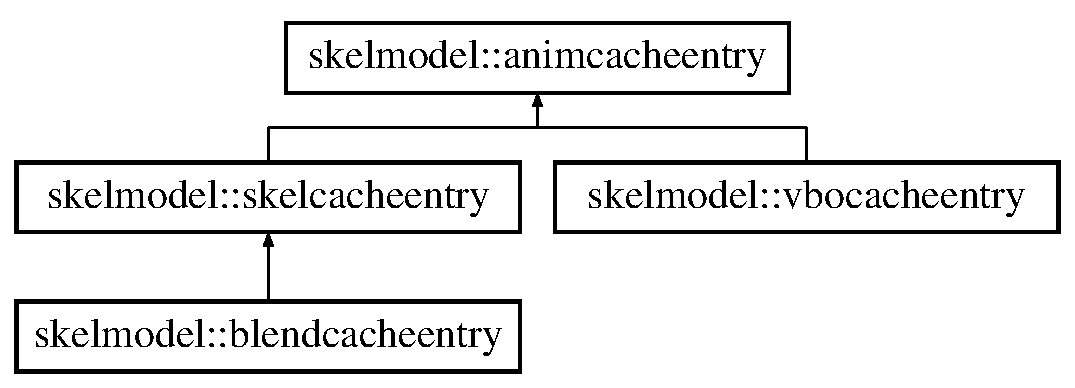
\includegraphics[height=3.000000cm]{structskelmodel_1_1animcacheentry}
\end{center}
\end{figure}
\subsection*{Public Member Functions}
\begin{DoxyCompactItemize}
\item 
\mbox{\Hypertarget{structskelmodel_1_1animcacheentry_a4fe8efdca5b85d720bcd73e3fc0791d0}\label{structskelmodel_1_1animcacheentry_a4fe8efdca5b85d720bcd73e3fc0791d0}} 
bool {\bfseries operator==} (const \hyperlink{structskelmodel_1_1animcacheentry}{animcacheentry} \&c) const
\item 
\mbox{\Hypertarget{structskelmodel_1_1animcacheentry_a33723521ed91c43b0ec9403f01848e3a}\label{structskelmodel_1_1animcacheentry_a33723521ed91c43b0ec9403f01848e3a}} 
bool {\bfseries operator!=} (const \hyperlink{structskelmodel_1_1animcacheentry}{animcacheentry} \&c) const
\end{DoxyCompactItemize}
\subsection*{Public Attributes}
\begin{DoxyCompactItemize}
\item 
\mbox{\Hypertarget{structskelmodel_1_1animcacheentry_ac28e0853d60f2171861d246b428251f0}\label{structskelmodel_1_1animcacheentry_ac28e0853d60f2171861d246b428251f0}} 
animstate {\bfseries as} \mbox{[}M\+A\+X\+A\+N\+I\+M\+P\+A\+R\+TS\mbox{]}
\item 
\mbox{\Hypertarget{structskelmodel_1_1animcacheentry_a127a9235fef9c158bde2847e7be09ea1}\label{structskelmodel_1_1animcacheentry_a127a9235fef9c158bde2847e7be09ea1}} 
float {\bfseries pitch}
\item 
\mbox{\Hypertarget{structskelmodel_1_1animcacheentry_a6044d26cdbe012c4ef8866d465c71181}\label{structskelmodel_1_1animcacheentry_a6044d26cdbe012c4ef8866d465c71181}} 
int {\bfseries millis}
\item 
\mbox{\Hypertarget{structskelmodel_1_1animcacheentry_a284612e43c86dfdb4d94e977cfe9b98d}\label{structskelmodel_1_1animcacheentry_a284612e43c86dfdb4d94e977cfe9b98d}} 
uchar $\ast$ {\bfseries partmask}
\item 
\mbox{\Hypertarget{structskelmodel_1_1animcacheentry_a75db1fb3885dae57b9e1f7d799b2fc91}\label{structskelmodel_1_1animcacheentry_a75db1fb3885dae57b9e1f7d799b2fc91}} 
\hyperlink{structragdolldata}{ragdolldata} $\ast$ {\bfseries ragdoll}
\end{DoxyCompactItemize}


The documentation for this struct was generated from the following file\+:\begin{DoxyCompactItemize}
\item 
H\+:/\+Rival\+Engine/\+Rival\+\_\+\+Game\+\_\+\+Engine\+\_\+\+G\+I\+T/\+Rival3dengine/source/engine/skelmodel.\+h\end{DoxyCompactItemize}

\hypertarget{structaniminfo}{}\section{animinfo Struct Reference}
\label{structaniminfo}\index{animinfo@{animinfo}}
\subsection*{Public Member Functions}
\begin{DoxyCompactItemize}
\item 
\mbox{\Hypertarget{structaniminfo_ad793c029705a3b7439ba5435b092ec94}\label{structaniminfo_ad793c029705a3b7439ba5435b092ec94}} 
bool {\bfseries operator==} (const \hyperlink{structaniminfo}{animinfo} \&o) const
\item 
\mbox{\Hypertarget{structaniminfo_ab5e8ce58ba8c1d755a1c60d9348cdf6d}\label{structaniminfo_ab5e8ce58ba8c1d755a1c60d9348cdf6d}} 
bool {\bfseries operator!=} (const \hyperlink{structaniminfo}{animinfo} \&o) const
\end{DoxyCompactItemize}
\subsection*{Public Attributes}
\begin{DoxyCompactItemize}
\item 
\mbox{\Hypertarget{structaniminfo_ab65d6d0e100929ab8e94fb1b4a150911}\label{structaniminfo_ab65d6d0e100929ab8e94fb1b4a150911}} 
int {\bfseries anim}
\item 
\mbox{\Hypertarget{structaniminfo_a2c6f216b77b1d5e484d7acb8b8d04e6c}\label{structaniminfo_a2c6f216b77b1d5e484d7acb8b8d04e6c}} 
int {\bfseries frame}
\item 
\mbox{\Hypertarget{structaniminfo_a4fb017dd4e6c951720cd4969eec13528}\label{structaniminfo_a4fb017dd4e6c951720cd4969eec13528}} 
int {\bfseries range}
\item 
\mbox{\Hypertarget{structaniminfo_a43bc563d24818f5bad8ae0a96c89b654}\label{structaniminfo_a43bc563d24818f5bad8ae0a96c89b654}} 
int {\bfseries basetime}
\item 
\mbox{\Hypertarget{structaniminfo_a064d4012692db2123ebcdd40d2a726cb}\label{structaniminfo_a064d4012692db2123ebcdd40d2a726cb}} 
float {\bfseries speed}
\item 
\mbox{\Hypertarget{structaniminfo_abc6bba14e97b6adcace6d95a6dbdd23a}\label{structaniminfo_abc6bba14e97b6adcace6d95a6dbdd23a}} 
uint {\bfseries varseed}
\end{DoxyCompactItemize}


The documentation for this struct was generated from the following file\+:\begin{DoxyCompactItemize}
\item 
H\+:/\+Rival\+Engine/\+Rival\+\_\+\+Game\+\_\+\+Engine\+\_\+\+G\+I\+T/\+Rival3dengine/source/shared/ents.\+h\end{DoxyCompactItemize}

\hypertarget{structaniminterpinfo}{}\section{animinterpinfo Struct Reference}
\label{structaniminterpinfo}\index{animinterpinfo@{animinterpinfo}}
\subsection*{Public Member Functions}
\begin{DoxyCompactItemize}
\item 
\mbox{\Hypertarget{structaniminterpinfo_af43e989185beeb83a4b7e376aaa69cc9}\label{structaniminterpinfo_af43e989185beeb83a4b7e376aaa69cc9}} 
void {\bfseries reset} ()
\end{DoxyCompactItemize}
\subsection*{Public Attributes}
\begin{DoxyCompactItemize}
\item 
\mbox{\Hypertarget{structaniminterpinfo_a0df901b788c8219e3e93d517c44e58b1}\label{structaniminterpinfo_a0df901b788c8219e3e93d517c44e58b1}} 
\hyperlink{structaniminfo}{animinfo} {\bfseries prev}
\item 
\mbox{\Hypertarget{structaniminterpinfo_af6df08fada2923854f195b4149a5f8d8}\label{structaniminterpinfo_af6df08fada2923854f195b4149a5f8d8}} 
\hyperlink{structaniminfo}{animinfo} {\bfseries cur}
\item 
\mbox{\Hypertarget{structaniminterpinfo_aec09f6afc6030dc489d12adf139b5b14}\label{structaniminterpinfo_aec09f6afc6030dc489d12adf139b5b14}} 
int {\bfseries lastswitch}
\item 
\mbox{\Hypertarget{structaniminterpinfo_a09a5934e6f553e187193739d3a256fba}\label{structaniminterpinfo_a09a5934e6f553e187193739d3a256fba}} 
void $\ast$ {\bfseries lastmodel}
\end{DoxyCompactItemize}


The documentation for this struct was generated from the following file\+:\begin{DoxyCompactItemize}
\item 
H\+:/\+Rival\+Engine/\+Rival\+\_\+\+Game\+\_\+\+Engine\+\_\+\+G\+I\+T/\+Rival3dengine/source/shared/ents.\+h\end{DoxyCompactItemize}

\hypertarget{structanimmodel}{}\section{animmodel Struct Reference}
\label{structanimmodel}\index{animmodel@{animmodel}}
Inheritance diagram for animmodel\+:\begin{figure}[H]
\begin{center}
\leavevmode
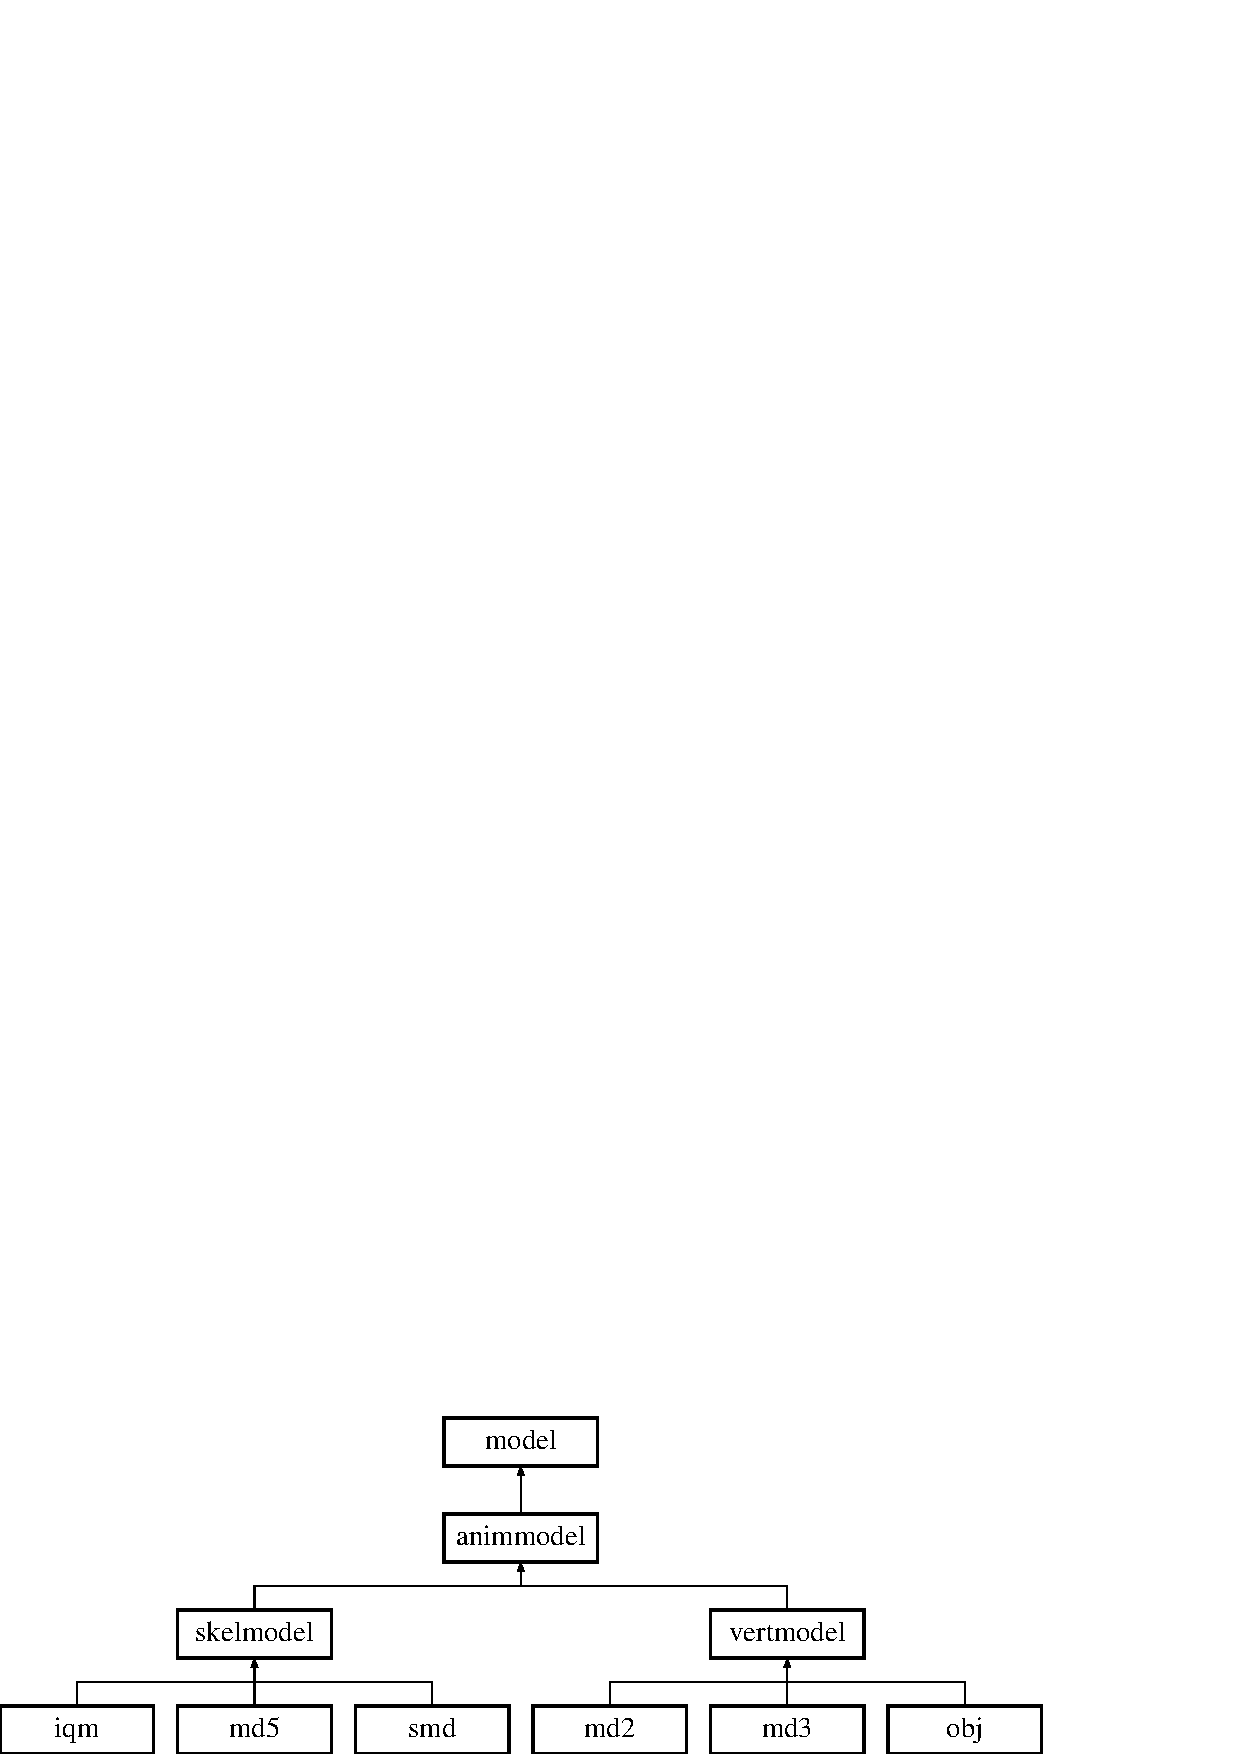
\includegraphics[height=4.000000cm]{structanimmodel}
\end{center}
\end{figure}
\subsection*{Classes}
\begin{DoxyCompactItemize}
\item 
struct \hyperlink{structanimmodel_1_1animpos}{animpos}
\item 
struct \hyperlink{structanimmodel_1_1animspec}{animspec}
\item 
struct \hyperlink{structanimmodel_1_1animstate}{animstate}
\item 
struct \hyperlink{structanimmodel_1_1linkedpart}{linkedpart}
\item 
struct \hyperlink{structanimmodel_1_1mesh}{mesh}
\item 
struct \hyperlink{structanimmodel_1_1meshgroup}{meshgroup}
\item 
struct \hyperlink{structanimmodel_1_1part}{part}
\item 
struct \hyperlink{structanimmodel_1_1shaderparams}{shaderparams}
\item 
struct \hyperlink{structanimmodel_1_1shaderparamskey}{shaderparamskey}
\item 
struct \hyperlink{structanimmodel_1_1skin}{skin}
\end{DoxyCompactItemize}
\subsection*{Public Types}
\begin{DoxyCompactItemize}
\item 
\mbox{\Hypertarget{structanimmodel_a3e4f076dbd12d38a1823dc852ebd4014}\label{structanimmodel_a3e4f076dbd12d38a1823dc852ebd4014}} 
enum \{ {\bfseries L\+I\+N\+K\+\_\+\+T\+AG} = 0, 
{\bfseries L\+I\+N\+K\+\_\+\+C\+O\+OP}, 
{\bfseries L\+I\+N\+K\+\_\+\+R\+E\+U\+SE}
 \}
\end{DoxyCompactItemize}
\subsection*{Public Member Functions}
\begin{DoxyCompactItemize}
\item 
\mbox{\Hypertarget{structanimmodel_a56b13dd7ec45bc5c07cd28e614a81982}\label{structanimmodel_a56b13dd7ec45bc5c07cd28e614a81982}} 
virtual int {\bfseries linktype} (\hyperlink{structanimmodel}{animmodel} $\ast$m, \hyperlink{structanimmodel_1_1part}{part} $\ast$p) const
\item 
\mbox{\Hypertarget{structanimmodel_ae3359d512c6c6c34e32ed98e9b8a51e7}\label{structanimmodel_ae3359d512c6c6c34e32ed98e9b8a51e7}} 
void {\bfseries intersect} (int anim, int basetime, int basetime2, float pitch, const \hyperlink{structvec}{vec} \&axis, const \hyperlink{structvec}{vec} \&forward, \hyperlink{structdynent}{dynent} $\ast$d, \hyperlink{structmodelattach}{modelattach} $\ast$a, const \hyperlink{structvec}{vec} \&o, const \hyperlink{structvec}{vec} \&ray)
\item 
\mbox{\Hypertarget{structanimmodel_a5bc10518c48616f2e1ee6eec4f2264a3}\label{structanimmodel_a5bc10518c48616f2e1ee6eec4f2264a3}} 
int {\bfseries intersect} (int anim, int basetime, int basetime2, const \hyperlink{structvec}{vec} \&pos, float yaw, float pitch, float roll, \hyperlink{structdynent}{dynent} $\ast$d, \hyperlink{structmodelattach}{modelattach} $\ast$a, float size, const \hyperlink{structvec}{vec} \&o, const \hyperlink{structvec}{vec} \&ray, float \&dist, int mode)
\item 
\mbox{\Hypertarget{structanimmodel_ac675f25eaaabe3c885dc56662b178036}\label{structanimmodel_ac675f25eaaabe3c885dc56662b178036}} 
void {\bfseries render} (int anim, int basetime, int basetime2, float pitch, const \hyperlink{structvec}{vec} \&axis, const \hyperlink{structvec}{vec} \&forward, \hyperlink{structdynent}{dynent} $\ast$d, \hyperlink{structmodelattach}{modelattach} $\ast$a)
\item 
\mbox{\Hypertarget{structanimmodel_a5e69cc0a64526b6b1abdcf1c14dfd3da}\label{structanimmodel_a5e69cc0a64526b6b1abdcf1c14dfd3da}} 
void {\bfseries render} (int anim, int basetime, int basetime2, const \hyperlink{structvec}{vec} \&o, float yaw, float pitch, float roll, \hyperlink{structdynent}{dynent} $\ast$d, \hyperlink{structmodelattach}{modelattach} $\ast$a, float size, const \hyperlink{structvec4}{vec4} \&color)
\item 
\mbox{\Hypertarget{structanimmodel_a4d6616ea5b740c69e9334aa87275753b}\label{structanimmodel_a4d6616ea5b740c69e9334aa87275753b}} 
{\bfseries animmodel} (const char $\ast$name)
\item 
\mbox{\Hypertarget{structanimmodel_a6d8d202b0542cb7474dd042158be618d}\label{structanimmodel_a6d8d202b0542cb7474dd042158be618d}} 
void {\bfseries cleanup} ()
\item 
\mbox{\Hypertarget{structanimmodel_af2c48bdb2cbbea0aef806093a0ea07fa}\label{structanimmodel_af2c48bdb2cbbea0aef806093a0ea07fa}} 
\hyperlink{structanimmodel_1_1part}{part} \& {\bfseries addpart} ()
\item 
\mbox{\Hypertarget{structanimmodel_ac65e188f24f9a408803e7173ddc07d16}\label{structanimmodel_ac65e188f24f9a408803e7173ddc07d16}} 
void {\bfseries initmatrix} (\hyperlink{structmatrix4x3}{matrix4x3} \&m)
\item 
\mbox{\Hypertarget{structanimmodel_acb1de49e303bdabbbf368f007f3d789f}\label{structanimmodel_acb1de49e303bdabbbf368f007f3d789f}} 
void {\bfseries gen\+B\+IH} (\hyperlink{structvector}{vector}$<$ \hyperlink{struct_b_i_h_1_1mesh}{B\+I\+H\+::mesh} $>$ \&bih)
\item 
\mbox{\Hypertarget{structanimmodel_a92fa053090b19aae9ad1b3cdf0745357}\label{structanimmodel_a92fa053090b19aae9ad1b3cdf0745357}} 
void {\bfseries genshadowmesh} (\hyperlink{structvector}{vector}$<$ \hyperlink{structtriangle}{triangle} $>$ \&tris, const \hyperlink{structmatrix4x3}{matrix4x3} \&orient)
\item 
\mbox{\Hypertarget{structanimmodel_ad493436cb56e10676a3d6f236fdb0e9c}\label{structanimmodel_ad493436cb56e10676a3d6f236fdb0e9c}} 
void {\bfseries preload\+B\+IH} ()
\item 
\mbox{\Hypertarget{structanimmodel_a1a7cb08383b1c5feefc728589561727a}\label{structanimmodel_a1a7cb08383b1c5feefc728589561727a}} 
\hyperlink{struct_b_i_h}{B\+IH} $\ast$ {\bfseries set\+B\+IH} ()
\item 
\mbox{\Hypertarget{structanimmodel_abb2471c627f61b3f1fb8ae67b116b3a5}\label{structanimmodel_abb2471c627f61b3f1fb8ae67b116b3a5}} 
bool {\bfseries link} (\hyperlink{structanimmodel_1_1part}{part} $\ast$p, const char $\ast$tag, const \hyperlink{structvec}{vec} \&translate=\hyperlink{structvec}{vec}(0, 0, 0), int anim=-\/1, int basetime=0, \hyperlink{structvec}{vec} $\ast$pos=N\+U\+LL)
\item 
\mbox{\Hypertarget{structanimmodel_a295c5ddbe03acab89bf0d887ba1474a8}\label{structanimmodel_a295c5ddbe03acab89bf0d887ba1474a8}} 
bool {\bfseries unlink} (\hyperlink{structanimmodel_1_1part}{part} $\ast$p)
\item 
\mbox{\Hypertarget{structanimmodel_a38a471f7e4559b46b906d6aa2c8c9adc}\label{structanimmodel_a38a471f7e4559b46b906d6aa2c8c9adc}} 
bool {\bfseries envmapped} () const
\item 
\mbox{\Hypertarget{structanimmodel_ad99da445d72fe4fd3410b0f43dd1b320}\label{structanimmodel_ad99da445d72fe4fd3410b0f43dd1b320}} 
bool {\bfseries animated} () const
\item 
\mbox{\Hypertarget{structanimmodel_af4a1ee0f2c2538adcfabaa661e985a8e}\label{structanimmodel_af4a1ee0f2c2538adcfabaa661e985a8e}} 
bool {\bfseries pitched} () const
\item 
\mbox{\Hypertarget{structanimmodel_a0a2b25cfbe1b7f6428eb2154c121a213}\label{structanimmodel_a0a2b25cfbe1b7f6428eb2154c121a213}} 
bool {\bfseries alphatested} () const
\item 
\mbox{\Hypertarget{structanimmodel_a1e5da2a8ebbdb7df6bc046b335be532b}\label{structanimmodel_a1e5da2a8ebbdb7df6bc046b335be532b}} 
virtual bool {\bfseries loaddefaultparts} ()
\item 
\mbox{\Hypertarget{structanimmodel_aaeb99e417a2a13f7fd6314ea8ddee580}\label{structanimmodel_aaeb99e417a2a13f7fd6314ea8ddee580}} 
void {\bfseries preloadshaders} ()
\item 
\mbox{\Hypertarget{structanimmodel_a56469b961b6615fb54302057a8822d12}\label{structanimmodel_a56469b961b6615fb54302057a8822d12}} 
void {\bfseries preloadmeshes} ()
\item 
\mbox{\Hypertarget{structanimmodel_a16f1da27ad68b0abef99b59099642b39}\label{structanimmodel_a16f1da27ad68b0abef99b59099642b39}} 
void {\bfseries setshader} (\hyperlink{struct_shader}{Shader} $\ast$shader)
\item 
\mbox{\Hypertarget{structanimmodel_ad5bd262a068d21a9c062707709d5c000}\label{structanimmodel_ad5bd262a068d21a9c062707709d5c000}} 
void {\bfseries setenvmap} (float envmapmin, float envmapmax, \hyperlink{struct_texture}{Texture} $\ast$\hyperlink{structenvmap}{envmap})
\item 
\mbox{\Hypertarget{structanimmodel_a38d13767831a8a38197b66bab3385bbd}\label{structanimmodel_a38d13767831a8a38197b66bab3385bbd}} 
void {\bfseries setspec} (float spec)
\item 
\mbox{\Hypertarget{structanimmodel_a97731333f3a91102f4e3a1719050ce19}\label{structanimmodel_a97731333f3a91102f4e3a1719050ce19}} 
void {\bfseries setgloss} (int gloss)
\item 
\mbox{\Hypertarget{structanimmodel_aba40170504ff95a3fcfd5376bec1f4cf}\label{structanimmodel_aba40170504ff95a3fcfd5376bec1f4cf}} 
void {\bfseries setglow} (float glow, float delta, float pulse)
\item 
\mbox{\Hypertarget{structanimmodel_a0bc1ea2c24f576e241060c33595db43f}\label{structanimmodel_a0bc1ea2c24f576e241060c33595db43f}} 
void {\bfseries setalphatest} (float alphatest)
\item 
\mbox{\Hypertarget{structanimmodel_acaca8dba6909d0ed2cf02095baac0fa4}\label{structanimmodel_acaca8dba6909d0ed2cf02095baac0fa4}} 
void {\bfseries setfullbright} (float fullbright)
\item 
\mbox{\Hypertarget{structanimmodel_a4e172eba82417aefa5765edb2503c2be}\label{structanimmodel_a4e172eba82417aefa5765edb2503c2be}} 
void {\bfseries setcullface} (bool cullface)
\item 
\mbox{\Hypertarget{structanimmodel_ada194ea26cf44d12c873db81da8e7c57}\label{structanimmodel_ada194ea26cf44d12c873db81da8e7c57}} 
void {\bfseries setcolor} (const \hyperlink{structvec}{vec} \&color)
\item 
\mbox{\Hypertarget{structanimmodel_a7b0919a98d2e2c78f8c8afd67fdd3fc2}\label{structanimmodel_a7b0919a98d2e2c78f8c8afd67fdd3fc2}} 
void {\bfseries setparascale} (const \hyperlink{structvec}{vec} \&parascale)
\item 
\mbox{\Hypertarget{structanimmodel_a1f5ff7713f5429521fa935962947e7fb}\label{structanimmodel_a1f5ff7713f5429521fa935962947e7fb}} 
void {\bfseries calcbb} (\hyperlink{structvec}{vec} \&center, \hyperlink{structvec}{vec} \&radius)
\item 
\mbox{\Hypertarget{structanimmodel_a135985486337c45bdb24c4e71ef704a4}\label{structanimmodel_a135985486337c45bdb24c4e71ef704a4}} 
void {\bfseries calctransform} (\hyperlink{structmatrix4x3}{matrix4x3} \&m)
\item 
\mbox{\Hypertarget{structanimmodel_a2286209e8ac8023894deabc008e851c6}\label{structanimmodel_a2286209e8ac8023894deabc008e851c6}} 
virtual void {\bfseries loaded} ()
\item 
\mbox{\Hypertarget{structanimmodel_aa31164f6d65fa63b2a648218b027692e}\label{structanimmodel_aa31164f6d65fa63b2a648218b027692e}} 
void {\bfseries startrender} ()
\item 
\mbox{\Hypertarget{structanimmodel_abb05af72648b8abd5fd7d8683751bb82}\label{structanimmodel_abb05af72648b8abd5fd7d8683751bb82}} 
void {\bfseries endrender} ()
\end{DoxyCompactItemize}
\subsection*{Static Public Member Functions}
\begin{DoxyCompactItemize}
\item 
\mbox{\Hypertarget{structanimmodel_a292961d8709679a14340cf3c3068ef6a}\label{structanimmodel_a292961d8709679a14340cf3c3068ef6a}} 
static void {\bfseries disablebones} ()
\item 
\mbox{\Hypertarget{structanimmodel_a943cf15df5f77f3eb757c4b8034fe51f}\label{structanimmodel_a943cf15df5f77f3eb757c4b8034fe51f}} 
static void {\bfseries disabletangents} ()
\item 
\mbox{\Hypertarget{structanimmodel_a6f54e99a87cbdf411e425f25bd9e7335}\label{structanimmodel_a6f54e99a87cbdf411e425f25bd9e7335}} 
static void {\bfseries disabletc} ()
\item 
\mbox{\Hypertarget{structanimmodel_a4534bf9318c152d8d9c41c6be15e3a87}\label{structanimmodel_a4534bf9318c152d8d9c41c6be15e3a87}} 
static void {\bfseries disablevbo} ()
\end{DoxyCompactItemize}
\subsection*{Public Attributes}
\begin{DoxyCompactItemize}
\item 
\mbox{\Hypertarget{structanimmodel_a41c52c3feba8bec721c71ff93db11c4a}\label{structanimmodel_a41c52c3feba8bec721c71ff93db11c4a}} 
\hyperlink{structvector}{vector}$<$ \hyperlink{structanimmodel_1_1part}{part} $\ast$ $>$ {\bfseries parts}
\end{DoxyCompactItemize}
\subsection*{Static Public Attributes}
\begin{DoxyCompactItemize}
\item 
\mbox{\Hypertarget{structanimmodel_a181da0ce12df773f0de1a1d898273f37}\label{structanimmodel_a181da0ce12df773f0de1a1d898273f37}} 
static \hyperlink{structhashnameset}{hashnameset}$<$ \hyperlink{structanimmodel_1_1meshgroup}{meshgroup} $\ast$ $>$ {\bfseries meshgroups}
\item 
\mbox{\Hypertarget{structanimmodel_ac74538f269270334cf403c697624f3fb}\label{structanimmodel_ac74538f269270334cf403c697624f3fb}} 
static int {\bfseries intersectresult} = -\/1
\item 
\mbox{\Hypertarget{structanimmodel_ac094dcd7721756ef3c3091c278896327}\label{structanimmodel_ac094dcd7721756ef3c3091c278896327}} 
static int {\bfseries intersectmode} = 0
\item 
\mbox{\Hypertarget{structanimmodel_a4065ef765537c60c20811d2d42bad0c7}\label{structanimmodel_a4065ef765537c60c20811d2d42bad0c7}} 
static float {\bfseries intersectdist} = 0
\item 
\mbox{\Hypertarget{structanimmodel_a74c1c90c044a25d6d343ef00f24932b7}\label{structanimmodel_a74c1c90c044a25d6d343ef00f24932b7}} 
static float {\bfseries intersectscale} = 1
\item 
\mbox{\Hypertarget{structanimmodel_a9b4ab567a3f007b99d8088360f68d625}\label{structanimmodel_a9b4ab567a3f007b99d8088360f68d625}} 
static bool {\bfseries enabletc} = false
\item 
\mbox{\Hypertarget{structanimmodel_a867aef2be2160bdef6e4c43ea5852a98}\label{structanimmodel_a867aef2be2160bdef6e4c43ea5852a98}} 
static bool {\bfseries enablecullface} = true
\item 
\mbox{\Hypertarget{structanimmodel_a914a36c32c8243c35e638082cc144f2f}\label{structanimmodel_a914a36c32c8243c35e638082cc144f2f}} 
static bool {\bfseries enabletangents} = false
\item 
\mbox{\Hypertarget{structanimmodel_abdbbd486c1faab279c4f9e9e3180402a}\label{structanimmodel_abdbbd486c1faab279c4f9e9e3180402a}} 
static bool {\bfseries enablebones} = false
\item 
\mbox{\Hypertarget{structanimmodel_a0f5336b1cdf6c0cad6847711aa5871dc}\label{structanimmodel_a0f5336b1cdf6c0cad6847711aa5871dc}} 
static bool {\bfseries enabledepthoffset} = false
\item 
\mbox{\Hypertarget{structanimmodel_a1fdc449ca9c5be2ebcfe8554c4152afa}\label{structanimmodel_a1fdc449ca9c5be2ebcfe8554c4152afa}} 
static float {\bfseries sizescale} = 1
\item 
\mbox{\Hypertarget{structanimmodel_a73568f03b8a48a7faaab4d3fadcbb6b4}\label{structanimmodel_a73568f03b8a48a7faaab4d3fadcbb6b4}} 
static \hyperlink{structvec4}{vec4} {\bfseries colorscale}
\item 
\mbox{\Hypertarget{structanimmodel_af46c4e0f235fb107c285312aabfeaece}\label{structanimmodel_af46c4e0f235fb107c285312aabfeaece}} 
static G\+Luint {\bfseries lastvbuf} = 0
\item 
\mbox{\Hypertarget{structanimmodel_a6dc60ef2f0d3f5425c2ffe343560cce4}\label{structanimmodel_a6dc60ef2f0d3f5425c2ffe343560cce4}} 
static G\+Luint {\bfseries lasttcbuf} = 0
\item 
\mbox{\Hypertarget{structanimmodel_aca71419af31202d59f3fce515a97746b}\label{structanimmodel_aca71419af31202d59f3fce515a97746b}} 
static G\+Luint {\bfseries lastxbuf} = 0
\item 
\mbox{\Hypertarget{structanimmodel_a7d16f7d6f815765f39a74b55cce84fb9}\label{structanimmodel_a7d16f7d6f815765f39a74b55cce84fb9}} 
static G\+Luint {\bfseries lastbbuf} = 0
\item 
\mbox{\Hypertarget{structanimmodel_a5141f8f6a6f5e0ee4aacf7fdd8628c11}\label{structanimmodel_a5141f8f6a6f5e0ee4aacf7fdd8628c11}} 
static G\+Luint {\bfseries lastebuf} = 0
\item 
\mbox{\Hypertarget{structanimmodel_ada80e5372157f77eb623159cf3b2ee50}\label{structanimmodel_ada80e5372157f77eb623159cf3b2ee50}} 
static G\+Luint {\bfseries lastenvmaptex} = 0
\item 
\mbox{\Hypertarget{structanimmodel_aac2c4f2debeb7d03a0f646a6745c1f1e}\label{structanimmodel_aac2c4f2debeb7d03a0f646a6745c1f1e}} 
static G\+Luint {\bfseries closestenvmaptex} = 0
\item 
\mbox{\Hypertarget{structanimmodel_a4e253188a6d69f01bc0c309880513639}\label{structanimmodel_a4e253188a6d69f01bc0c309880513639}} 
static \hyperlink{struct_texture}{Texture} $\ast$ {\bfseries lasttex} = N\+U\+LL
\item 
\mbox{\Hypertarget{structanimmodel_a0c3d40b3c61542906e091885cc9a52f0}\label{structanimmodel_a0c3d40b3c61542906e091885cc9a52f0}} 
static \hyperlink{struct_texture}{Texture} $\ast$ {\bfseries lastdecal} = N\+U\+LL
\item 
\mbox{\Hypertarget{structanimmodel_ac72ea00d8fb6f05bed6b9a8e7c888c5a}\label{structanimmodel_ac72ea00d8fb6f05bed6b9a8e7c888c5a}} 
static \hyperlink{struct_texture}{Texture} $\ast$ {\bfseries lastmasks} = N\+U\+LL
\item 
\mbox{\Hypertarget{structanimmodel_a4aa5b2a84482b23846f662351eac7a54}\label{structanimmodel_a4aa5b2a84482b23846f662351eac7a54}} 
static \hyperlink{struct_texture}{Texture} $\ast$ {\bfseries lastnormalmap} = N\+U\+LL
\item 
\mbox{\Hypertarget{structanimmodel_ac496317c2c1b464951b9a28dac25e31b}\label{structanimmodel_ac496317c2c1b464951b9a28dac25e31b}} 
static int {\bfseries matrixpos} = 0
\item 
\mbox{\Hypertarget{structanimmodel_abdb8d4166cedcdba6e6be96b3b29022f}\label{structanimmodel_abdb8d4166cedcdba6e6be96b3b29022f}} 
static \hyperlink{structmatrix4}{matrix4} {\bfseries matrixstack} \mbox{[}64\mbox{]}
\end{DoxyCompactItemize}


The documentation for this struct was generated from the following file\+:\begin{DoxyCompactItemize}
\item 
H\+:/\+Rival\+Engine/\+Rival\+\_\+\+Game\+\_\+\+Engine\+\_\+\+G\+I\+T/\+Rival3dengine/source/engine/animmodel.\+h\end{DoxyCompactItemize}

\hypertarget{structskelmodel_1_1animpartmask}{}\section{skelmodel\+:\+:animpartmask Struct Reference}
\label{structskelmodel_1_1animpartmask}\index{skelmodel\+::animpartmask@{skelmodel\+::animpartmask}}
\subsection*{Public Attributes}
\begin{DoxyCompactItemize}
\item 
\mbox{\Hypertarget{structskelmodel_1_1animpartmask_aa58b9140ef3f62c955c9fc145d1213f8}\label{structskelmodel_1_1animpartmask_aa58b9140ef3f62c955c9fc145d1213f8}} 
\hyperlink{structskelmodel_1_1animpartmask}{animpartmask} $\ast$ {\bfseries next}
\item 
\mbox{\Hypertarget{structskelmodel_1_1animpartmask_a0286cde18fcb4ebe8c94a271126fb7f9}\label{structskelmodel_1_1animpartmask_a0286cde18fcb4ebe8c94a271126fb7f9}} 
int {\bfseries numbones}
\item 
\mbox{\Hypertarget{structskelmodel_1_1animpartmask_ae891651a4368e0766a6a29750fb4d9ba}\label{structskelmodel_1_1animpartmask_ae891651a4368e0766a6a29750fb4d9ba}} 
uchar {\bfseries bones} \mbox{[}1\mbox{]}
\end{DoxyCompactItemize}


The documentation for this struct was generated from the following file\+:\begin{DoxyCompactItemize}
\item 
H\+:/\+Rival\+Engine/\+Rival\+\_\+\+Game\+\_\+\+Engine\+\_\+\+G\+I\+T/\+Rival3dengine/source/engine/skelmodel.\+h\end{DoxyCompactItemize}

\hypertarget{structanimmodel_1_1animpos}{}\section{animmodel\+:\+:animpos Struct Reference}
\label{structanimmodel_1_1animpos}\index{animmodel\+::animpos@{animmodel\+::animpos}}
\subsection*{Public Member Functions}
\begin{DoxyCompactItemize}
\item 
\mbox{\Hypertarget{structanimmodel_1_1animpos_aa5723e46e6e5f17e9d2eb978bdec8cfd}\label{structanimmodel_1_1animpos_aa5723e46e6e5f17e9d2eb978bdec8cfd}} 
void {\bfseries setframes} (const \hyperlink{structaniminfo}{animinfo} \&info)
\item 
\mbox{\Hypertarget{structanimmodel_1_1animpos_ae5fd4719d19503408a7c8a10c3cc516c}\label{structanimmodel_1_1animpos_ae5fd4719d19503408a7c8a10c3cc516c}} 
bool {\bfseries operator==} (const \hyperlink{structanimmodel_1_1animpos}{animpos} \&a) const
\item 
\mbox{\Hypertarget{structanimmodel_1_1animpos_a251861f2551eb5cd53544cb362c01e3a}\label{structanimmodel_1_1animpos_a251861f2551eb5cd53544cb362c01e3a}} 
bool {\bfseries operator!=} (const \hyperlink{structanimmodel_1_1animpos}{animpos} \&a) const
\end{DoxyCompactItemize}
\subsection*{Public Attributes}
\begin{DoxyCompactItemize}
\item 
\mbox{\Hypertarget{structanimmodel_1_1animpos_a740becfa376f8c7f03065e4815cfb1b3}\label{structanimmodel_1_1animpos_a740becfa376f8c7f03065e4815cfb1b3}} 
int {\bfseries anim}
\item 
\mbox{\Hypertarget{structanimmodel_1_1animpos_a188a93230cec192000d2a49113a2afdc}\label{structanimmodel_1_1animpos_a188a93230cec192000d2a49113a2afdc}} 
int {\bfseries fr1}
\item 
\mbox{\Hypertarget{structanimmodel_1_1animpos_ae796f792d1983ee48d0182d63057ef6c}\label{structanimmodel_1_1animpos_ae796f792d1983ee48d0182d63057ef6c}} 
int {\bfseries fr2}
\item 
\mbox{\Hypertarget{structanimmodel_1_1animpos_ae7340830bcb39bbea5c95ee9059fcd8d}\label{structanimmodel_1_1animpos_ae7340830bcb39bbea5c95ee9059fcd8d}} 
float {\bfseries t}
\end{DoxyCompactItemize}


The documentation for this struct was generated from the following file\+:\begin{DoxyCompactItemize}
\item 
H\+:/\+Rival\+Engine/\+Rival\+\_\+\+Game\+\_\+\+Engine\+\_\+\+G\+I\+T/\+Rival3dengine/source/engine/animmodel.\+h\end{DoxyCompactItemize}

\hypertarget{structanimmodel_1_1animspec}{}\section{animmodel\+:\+:animspec Struct Reference}
\label{structanimmodel_1_1animspec}\index{animmodel\+::animspec@{animmodel\+::animspec}}
\subsection*{Public Attributes}
\begin{DoxyCompactItemize}
\item 
\mbox{\Hypertarget{structanimmodel_1_1animspec_acab48550aa1e9a2e4fd2e3a6891c738d}\label{structanimmodel_1_1animspec_acab48550aa1e9a2e4fd2e3a6891c738d}} 
int {\bfseries frame}
\item 
\mbox{\Hypertarget{structanimmodel_1_1animspec_a36f5f5faa201eaa4073bc487d3fba138}\label{structanimmodel_1_1animspec_a36f5f5faa201eaa4073bc487d3fba138}} 
int {\bfseries range}
\item 
\mbox{\Hypertarget{structanimmodel_1_1animspec_a40ce587fca55bd1e2c89f9f961551e89}\label{structanimmodel_1_1animspec_a40ce587fca55bd1e2c89f9f961551e89}} 
float {\bfseries speed}
\item 
\mbox{\Hypertarget{structanimmodel_1_1animspec_ae45450fdabf29ebf6a10cfb0d7e4f52c}\label{structanimmodel_1_1animspec_ae45450fdabf29ebf6a10cfb0d7e4f52c}} 
int {\bfseries priority}
\end{DoxyCompactItemize}


The documentation for this struct was generated from the following file\+:\begin{DoxyCompactItemize}
\item 
H\+:/\+Rival\+Engine/\+Rival\+\_\+\+Game\+\_\+\+Engine\+\_\+\+G\+I\+T/\+Rival3dengine/source/engine/animmodel.\+h\end{DoxyCompactItemize}

\hypertarget{structanimmodel_1_1animstate}{}\section{animmodel\+:\+:animstate Struct Reference}
\label{structanimmodel_1_1animstate}\index{animmodel\+::animstate@{animmodel\+::animstate}}
\subsection*{Public Member Functions}
\begin{DoxyCompactItemize}
\item 
\mbox{\Hypertarget{structanimmodel_1_1animstate_a4c070cf8d156f6b0d4ed807b5de5d0d2}\label{structanimmodel_1_1animstate_a4c070cf8d156f6b0d4ed807b5de5d0d2}} 
bool {\bfseries operator==} (const \hyperlink{structanimmodel_1_1animstate}{animstate} \&a) const
\item 
\mbox{\Hypertarget{structanimmodel_1_1animstate_a847fb5c99a1b373a7ddb1e771d709dfc}\label{structanimmodel_1_1animstate_a847fb5c99a1b373a7ddb1e771d709dfc}} 
bool {\bfseries operator!=} (const \hyperlink{structanimmodel_1_1animstate}{animstate} \&a) const
\end{DoxyCompactItemize}
\subsection*{Public Attributes}
\begin{DoxyCompactItemize}
\item 
\mbox{\Hypertarget{structanimmodel_1_1animstate_ac017351f751938ec79cb173c7e95baf3}\label{structanimmodel_1_1animstate_ac017351f751938ec79cb173c7e95baf3}} 
\hyperlink{structanimmodel_1_1part}{part} $\ast$ {\bfseries owner}
\item 
\mbox{\Hypertarget{structanimmodel_1_1animstate_a0ab50671019e0beef50cdc6ceb5a137d}\label{structanimmodel_1_1animstate_a0ab50671019e0beef50cdc6ceb5a137d}} 
\hyperlink{structanimmodel_1_1animpos}{animpos} {\bfseries cur}
\item 
\mbox{\Hypertarget{structanimmodel_1_1animstate_ab4354f5ac989d48972d087a2b92d652a}\label{structanimmodel_1_1animstate_ab4354f5ac989d48972d087a2b92d652a}} 
\hyperlink{structanimmodel_1_1animpos}{animpos} {\bfseries prev}
\item 
\mbox{\Hypertarget{structanimmodel_1_1animstate_a515959fdd3c2579e6e172e26bab53700}\label{structanimmodel_1_1animstate_a515959fdd3c2579e6e172e26bab53700}} 
float {\bfseries interp}
\end{DoxyCompactItemize}


The documentation for this struct was generated from the following file\+:\begin{DoxyCompactItemize}
\item 
H\+:/\+Rival\+Engine/\+Rival\+\_\+\+Game\+\_\+\+Engine\+\_\+\+G\+I\+T/\+Rival3dengine/source/engine/animmodel.\+h\end{DoxyCompactItemize}

\hypertarget{structskelmodel_1_1antipode}{}\section{skelmodel\+:\+:antipode Struct Reference}
\label{structskelmodel_1_1antipode}\index{skelmodel\+::antipode@{skelmodel\+::antipode}}
\subsection*{Public Member Functions}
\begin{DoxyCompactItemize}
\item 
\mbox{\Hypertarget{structskelmodel_1_1antipode_a43a1e6da9d214c146dee2d3bd9fc6642}\label{structskelmodel_1_1antipode_a43a1e6da9d214c146dee2d3bd9fc6642}} 
{\bfseries antipode} (int parent, int child)
\end{DoxyCompactItemize}
\subsection*{Public Attributes}
\begin{DoxyCompactItemize}
\item 
\mbox{\Hypertarget{structskelmodel_1_1antipode_ae7fb042cd5d2e57df2532838934d73b4}\label{structskelmodel_1_1antipode_ae7fb042cd5d2e57df2532838934d73b4}} 
int {\bfseries parent}
\item 
\mbox{\Hypertarget{structskelmodel_1_1antipode_ae76395cd5641355c9ec936d1b415c308}\label{structskelmodel_1_1antipode_ae76395cd5641355c9ec936d1b415c308}} 
int {\bfseries child}
\end{DoxyCompactItemize}


The documentation for this struct was generated from the following file\+:\begin{DoxyCompactItemize}
\item 
H\+:/\+Rival\+Engine/\+Rival\+\_\+\+Game\+\_\+\+Engine\+\_\+\+G\+I\+T/\+Rival3dengine/source/engine/skelmodel.\+h\end{DoxyCompactItemize}

\hypertarget{classas_c_simple_dummy}{}\section{as\+C\+Simple\+Dummy Class Reference}
\label{classas_c_simple_dummy}\index{as\+C\+Simple\+Dummy@{as\+C\+Simple\+Dummy}}


The documentation for this class was generated from the following file\+:\begin{DoxyCompactItemize}
\item 
H\+:/\+Rival\+Engine/\+Rival\+\_\+\+Game\+\_\+\+Engine\+\_\+\+G\+I\+T/\+Rival3dengine/source/engine/angelscript.\+h\end{DoxyCompactItemize}

\hypertarget{classas_i_binary_stream}{}\section{as\+I\+Binary\+Stream Class Reference}
\label{classas_i_binary_stream}\index{as\+I\+Binary\+Stream@{as\+I\+Binary\+Stream}}
\subsection*{Public Member Functions}
\begin{DoxyCompactItemize}
\item 
\mbox{\Hypertarget{classas_i_binary_stream_ab69b772db0a4157a842d90070e6fa1dc}\label{classas_i_binary_stream_ab69b772db0a4157a842d90070e6fa1dc}} 
virtual void {\bfseries Read} (void $\ast$ptr, as\+U\+I\+NT size)=0
\item 
\mbox{\Hypertarget{classas_i_binary_stream_a1fce5bbea004d6b2705f9eefae1a3770}\label{classas_i_binary_stream_a1fce5bbea004d6b2705f9eefae1a3770}} 
virtual void {\bfseries Write} (const void $\ast$ptr, as\+U\+I\+NT size)=0
\end{DoxyCompactItemize}


The documentation for this class was generated from the following file\+:\begin{DoxyCompactItemize}
\item 
H\+:/\+Rival\+Engine/\+Rival\+\_\+\+Game\+\_\+\+Engine\+\_\+\+G\+I\+T/\+Rival3dengine/source/engine/angelscript.\+h\end{DoxyCompactItemize}

\hypertarget{classas_i_j_i_t_compiler}{}\section{as\+I\+J\+I\+T\+Compiler Class Reference}
\label{classas_i_j_i_t_compiler}\index{as\+I\+J\+I\+T\+Compiler@{as\+I\+J\+I\+T\+Compiler}}
\subsection*{Public Member Functions}
\begin{DoxyCompactItemize}
\item 
\mbox{\Hypertarget{classas_i_j_i_t_compiler_aa6270727e61d8708d651a0f5faada695}\label{classas_i_j_i_t_compiler_aa6270727e61d8708d651a0f5faada695}} 
virtual int {\bfseries Compile\+Function} (\hyperlink{classas_i_script_function}{as\+I\+Script\+Function} $\ast$function, as\+J\+I\+T\+Function $\ast$output)=0
\item 
\mbox{\Hypertarget{classas_i_j_i_t_compiler_afbf9390868269c9224df85d49aabd451}\label{classas_i_j_i_t_compiler_afbf9390868269c9224df85d49aabd451}} 
virtual void {\bfseries Release\+J\+I\+T\+Function} (as\+J\+I\+T\+Function func)=0
\end{DoxyCompactItemize}


The documentation for this class was generated from the following file\+:\begin{DoxyCompactItemize}
\item 
H\+:/\+Rival\+Engine/\+Rival\+\_\+\+Game\+\_\+\+Engine\+\_\+\+G\+I\+T/\+Rival3dengine/source/engine/angelscript.\+h\end{DoxyCompactItemize}

\hypertarget{classas_i_lockable_shared_bool}{}\section{as\+I\+Lockable\+Shared\+Bool Class Reference}
\label{classas_i_lockable_shared_bool}\index{as\+I\+Lockable\+Shared\+Bool@{as\+I\+Lockable\+Shared\+Bool}}
\subsection*{Public Member Functions}
\begin{DoxyCompactItemize}
\item 
\mbox{\Hypertarget{classas_i_lockable_shared_bool_a1183742552ce6b952cc3742bd456d787}\label{classas_i_lockable_shared_bool_a1183742552ce6b952cc3742bd456d787}} 
virtual int {\bfseries Add\+Ref} () const =0
\item 
\mbox{\Hypertarget{classas_i_lockable_shared_bool_a1dae71f6f1141b5b16520232a9ea5fb2}\label{classas_i_lockable_shared_bool_a1dae71f6f1141b5b16520232a9ea5fb2}} 
virtual int {\bfseries Release} () const =0
\item 
\mbox{\Hypertarget{classas_i_lockable_shared_bool_abab39fc60f00ae8941423258ffc2c3c6}\label{classas_i_lockable_shared_bool_abab39fc60f00ae8941423258ffc2c3c6}} 
virtual bool {\bfseries Get} () const =0
\item 
\mbox{\Hypertarget{classas_i_lockable_shared_bool_aa29488ac2f1c38788d5e79545fdfc8c7}\label{classas_i_lockable_shared_bool_aa29488ac2f1c38788d5e79545fdfc8c7}} 
virtual void {\bfseries Set} (bool val)=0
\item 
\mbox{\Hypertarget{classas_i_lockable_shared_bool_aef12cc309395d682aa138da5eea9d82b}\label{classas_i_lockable_shared_bool_aef12cc309395d682aa138da5eea9d82b}} 
virtual void {\bfseries Lock} () const =0
\item 
\mbox{\Hypertarget{classas_i_lockable_shared_bool_a863984c1b271df84f71fb5ba978ce2b8}\label{classas_i_lockable_shared_bool_a863984c1b271df84f71fb5ba978ce2b8}} 
virtual void {\bfseries Unlock} () const =0
\end{DoxyCompactItemize}


The documentation for this class was generated from the following file\+:\begin{DoxyCompactItemize}
\item 
H\+:/\+Rival\+Engine/\+Rival\+\_\+\+Game\+\_\+\+Engine\+\_\+\+G\+I\+T/\+Rival3dengine/source/engine/angelscript.\+h\end{DoxyCompactItemize}

\hypertarget{classas_i_script_context}{}\section{as\+I\+Script\+Context Class Reference}
\label{classas_i_script_context}\index{as\+I\+Script\+Context@{as\+I\+Script\+Context}}
\subsection*{Public Member Functions}
\begin{DoxyCompactItemize}
\item 
\mbox{\Hypertarget{classas_i_script_context_a5e24f4cb5773f732a1d46b818d963a1d}\label{classas_i_script_context_a5e24f4cb5773f732a1d46b818d963a1d}} 
virtual int {\bfseries Add\+Ref} () const =0
\item 
\mbox{\Hypertarget{classas_i_script_context_a1b13a5f3e58627e9ff4300c0c6f0f3cf}\label{classas_i_script_context_a1b13a5f3e58627e9ff4300c0c6f0f3cf}} 
virtual int {\bfseries Release} () const =0
\item 
\mbox{\Hypertarget{classas_i_script_context_a07f12016c5435aec5b63449abb6e4d8d}\label{classas_i_script_context_a07f12016c5435aec5b63449abb6e4d8d}} 
virtual \hyperlink{classas_i_script_engine}{as\+I\+Script\+Engine} $\ast$ {\bfseries Get\+Engine} () const =0
\item 
\mbox{\Hypertarget{classas_i_script_context_a43976f42dfc6c1af23e132d36265173a}\label{classas_i_script_context_a43976f42dfc6c1af23e132d36265173a}} 
virtual int {\bfseries Prepare} (\hyperlink{classas_i_script_function}{as\+I\+Script\+Function} $\ast$func)=0
\item 
\mbox{\Hypertarget{classas_i_script_context_ae3c18a2cc66c56f840e6ee4310287f65}\label{classas_i_script_context_ae3c18a2cc66c56f840e6ee4310287f65}} 
virtual int {\bfseries Unprepare} ()=0
\item 
\mbox{\Hypertarget{classas_i_script_context_a8e52894432737acac2e1a422e496bf84}\label{classas_i_script_context_a8e52894432737acac2e1a422e496bf84}} 
virtual int {\bfseries Execute} ()=0
\item 
\mbox{\Hypertarget{classas_i_script_context_a374befd21b8c14de81ef0ed9d2dea334}\label{classas_i_script_context_a374befd21b8c14de81ef0ed9d2dea334}} 
virtual int {\bfseries Abort} ()=0
\item 
\mbox{\Hypertarget{classas_i_script_context_ad4ac8be3586c46069b5870e40c86544a}\label{classas_i_script_context_ad4ac8be3586c46069b5870e40c86544a}} 
virtual int {\bfseries Suspend} ()=0
\item 
\mbox{\Hypertarget{classas_i_script_context_a17024a9e1648f66711a3182b21676aa7}\label{classas_i_script_context_a17024a9e1648f66711a3182b21676aa7}} 
virtual as\+E\+Context\+State {\bfseries Get\+State} () const =0
\item 
\mbox{\Hypertarget{classas_i_script_context_ad8f7637a23d67e227d07f65621b6cdd6}\label{classas_i_script_context_ad8f7637a23d67e227d07f65621b6cdd6}} 
virtual int {\bfseries Push\+State} ()=0
\item 
\mbox{\Hypertarget{classas_i_script_context_a5d963974625e582799b5d911d182d9be}\label{classas_i_script_context_a5d963974625e582799b5d911d182d9be}} 
virtual int {\bfseries Pop\+State} ()=0
\item 
\mbox{\Hypertarget{classas_i_script_context_a378f3bbfa04ef7b806300c5d4f1a0d65}\label{classas_i_script_context_a378f3bbfa04ef7b806300c5d4f1a0d65}} 
virtual bool {\bfseries Is\+Nested} (as\+U\+I\+NT $\ast$nest\+Count=0) const =0
\item 
\mbox{\Hypertarget{classas_i_script_context_a10d3c152b25d07584999f4d9fe5ce8b1}\label{classas_i_script_context_a10d3c152b25d07584999f4d9fe5ce8b1}} 
virtual int {\bfseries Set\+Object} (void $\ast$\hyperlink{structobj}{obj})=0
\item 
\mbox{\Hypertarget{classas_i_script_context_ac5ac8ce5bb209f43d4da620db5d271da}\label{classas_i_script_context_ac5ac8ce5bb209f43d4da620db5d271da}} 
virtual int {\bfseries Set\+Arg\+Byte} (as\+U\+I\+NT arg, as\+B\+Y\+TE value)=0
\item 
\mbox{\Hypertarget{classas_i_script_context_ac882e19b922c681052a0a88d69289a47}\label{classas_i_script_context_ac882e19b922c681052a0a88d69289a47}} 
virtual int {\bfseries Set\+Arg\+Word} (as\+U\+I\+NT arg, as\+W\+O\+RD value)=0
\item 
\mbox{\Hypertarget{classas_i_script_context_a14cac831c1b419f552ca62a239dfcf45}\label{classas_i_script_context_a14cac831c1b419f552ca62a239dfcf45}} 
virtual int {\bfseries Set\+Arg\+D\+Word} (as\+U\+I\+NT arg, as\+D\+W\+O\+RD value)=0
\item 
\mbox{\Hypertarget{classas_i_script_context_a742c870360588e99528f09bae6156482}\label{classas_i_script_context_a742c870360588e99528f09bae6156482}} 
virtual int {\bfseries Set\+Arg\+Q\+Word} (as\+U\+I\+NT arg, as\+Q\+W\+O\+RD value)=0
\item 
\mbox{\Hypertarget{classas_i_script_context_a702a40cfe539e4e655a84e15161f8db8}\label{classas_i_script_context_a702a40cfe539e4e655a84e15161f8db8}} 
virtual int {\bfseries Set\+Arg\+Float} (as\+U\+I\+NT arg, float value)=0
\item 
\mbox{\Hypertarget{classas_i_script_context_acbdddda3b80c37b70b8fd35c8e7383b9}\label{classas_i_script_context_acbdddda3b80c37b70b8fd35c8e7383b9}} 
virtual int {\bfseries Set\+Arg\+Double} (as\+U\+I\+NT arg, double value)=0
\item 
\mbox{\Hypertarget{classas_i_script_context_aa8de8f21dfbb2cdf0becbabaa3e883ed}\label{classas_i_script_context_aa8de8f21dfbb2cdf0becbabaa3e883ed}} 
virtual int {\bfseries Set\+Arg\+Address} (as\+U\+I\+NT arg, void $\ast$addr)=0
\item 
\mbox{\Hypertarget{classas_i_script_context_a09044a12dfb2d44d19bd8a4025cb814d}\label{classas_i_script_context_a09044a12dfb2d44d19bd8a4025cb814d}} 
virtual int {\bfseries Set\+Arg\+Object} (as\+U\+I\+NT arg, void $\ast$\hyperlink{structobj}{obj})=0
\item 
\mbox{\Hypertarget{classas_i_script_context_a626d97ec564c92120e2abaf69f6e3698}\label{classas_i_script_context_a626d97ec564c92120e2abaf69f6e3698}} 
virtual int {\bfseries Set\+Arg\+Var\+Type} (as\+U\+I\+NT arg, void $\ast$ptr, int type\+Id)=0
\item 
\mbox{\Hypertarget{classas_i_script_context_a0fbab94982862b30cd55996d4a24949c}\label{classas_i_script_context_a0fbab94982862b30cd55996d4a24949c}} 
virtual void $\ast$ {\bfseries Get\+Address\+Of\+Arg} (as\+U\+I\+NT arg)=0
\item 
\mbox{\Hypertarget{classas_i_script_context_a4c92259c03f1394310d3ea7d0774b3cb}\label{classas_i_script_context_a4c92259c03f1394310d3ea7d0774b3cb}} 
virtual as\+B\+Y\+TE {\bfseries Get\+Return\+Byte} ()=0
\item 
\mbox{\Hypertarget{classas_i_script_context_a5a3e054d35a6a361af67448d0a4930f9}\label{classas_i_script_context_a5a3e054d35a6a361af67448d0a4930f9}} 
virtual as\+W\+O\+RD {\bfseries Get\+Return\+Word} ()=0
\item 
\mbox{\Hypertarget{classas_i_script_context_a43cd2fb72685aef96e8ddc622c9621bf}\label{classas_i_script_context_a43cd2fb72685aef96e8ddc622c9621bf}} 
virtual as\+D\+W\+O\+RD {\bfseries Get\+Return\+D\+Word} ()=0
\item 
\mbox{\Hypertarget{classas_i_script_context_a22bdd3b67dee3b1dbcb3f9f9a1f21fa4}\label{classas_i_script_context_a22bdd3b67dee3b1dbcb3f9f9a1f21fa4}} 
virtual as\+Q\+W\+O\+RD {\bfseries Get\+Return\+Q\+Word} ()=0
\item 
\mbox{\Hypertarget{classas_i_script_context_a4ad325995e43fe6a929bcbd8fa592500}\label{classas_i_script_context_a4ad325995e43fe6a929bcbd8fa592500}} 
virtual float {\bfseries Get\+Return\+Float} ()=0
\item 
\mbox{\Hypertarget{classas_i_script_context_a7e1ce03637cd5dd48ea652fdf7913bd7}\label{classas_i_script_context_a7e1ce03637cd5dd48ea652fdf7913bd7}} 
virtual double {\bfseries Get\+Return\+Double} ()=0
\item 
\mbox{\Hypertarget{classas_i_script_context_a2438a7fcf46faa2267bdb94057cd1f2e}\label{classas_i_script_context_a2438a7fcf46faa2267bdb94057cd1f2e}} 
virtual void $\ast$ {\bfseries Get\+Return\+Address} ()=0
\item 
\mbox{\Hypertarget{classas_i_script_context_a6d5739fac9c90bcd0fea55d01841d43a}\label{classas_i_script_context_a6d5739fac9c90bcd0fea55d01841d43a}} 
virtual void $\ast$ {\bfseries Get\+Return\+Object} ()=0
\item 
\mbox{\Hypertarget{classas_i_script_context_a889bf11123beba669637849c8e9b2b86}\label{classas_i_script_context_a889bf11123beba669637849c8e9b2b86}} 
virtual void $\ast$ {\bfseries Get\+Address\+Of\+Return\+Value} ()=0
\item 
\mbox{\Hypertarget{classas_i_script_context_a4ed608208cafdebe5676df079e27d392}\label{classas_i_script_context_a4ed608208cafdebe5676df079e27d392}} 
virtual int {\bfseries Set\+Exception} (const char $\ast$string)=0
\item 
\mbox{\Hypertarget{classas_i_script_context_a22e3c351fe6b13ba0a62010dfc305080}\label{classas_i_script_context_a22e3c351fe6b13ba0a62010dfc305080}} 
virtual int {\bfseries Get\+Exception\+Line\+Number} (int $\ast$column=0, const char $\ast$$\ast$section\+Name=0)=0
\item 
\mbox{\Hypertarget{classas_i_script_context_a8e59aceec42080d29e08b44460ceb8b3}\label{classas_i_script_context_a8e59aceec42080d29e08b44460ceb8b3}} 
virtual \hyperlink{classas_i_script_function}{as\+I\+Script\+Function} $\ast$ {\bfseries Get\+Exception\+Function} ()=0
\item 
\mbox{\Hypertarget{classas_i_script_context_a46e2411bc84e99f57e7d9fe2374bb479}\label{classas_i_script_context_a46e2411bc84e99f57e7d9fe2374bb479}} 
virtual const char $\ast$ {\bfseries Get\+Exception\+String} ()=0
\item 
\mbox{\Hypertarget{classas_i_script_context_a4d1f481473df3f7aefccc5bb6904e405}\label{classas_i_script_context_a4d1f481473df3f7aefccc5bb6904e405}} 
virtual int {\bfseries Set\+Exception\+Callback} (\hyperlink{structas_s_func_ptr}{as\+S\+Func\+Ptr} callback, void $\ast$\hyperlink{structobj}{obj}, int call\+Conv)=0
\item 
\mbox{\Hypertarget{classas_i_script_context_acb5cfe5703031fd76672a57d8afae547}\label{classas_i_script_context_acb5cfe5703031fd76672a57d8afae547}} 
virtual void {\bfseries Clear\+Exception\+Callback} ()=0
\item 
\mbox{\Hypertarget{classas_i_script_context_ae2747f643bf9a07364f922c460ef57dd}\label{classas_i_script_context_ae2747f643bf9a07364f922c460ef57dd}} 
virtual int {\bfseries Set\+Line\+Callback} (\hyperlink{structas_s_func_ptr}{as\+S\+Func\+Ptr} callback, void $\ast$\hyperlink{structobj}{obj}, int call\+Conv)=0
\item 
\mbox{\Hypertarget{classas_i_script_context_a3771cf314de339fa5d70edfbfcd88370}\label{classas_i_script_context_a3771cf314de339fa5d70edfbfcd88370}} 
virtual void {\bfseries Clear\+Line\+Callback} ()=0
\item 
\mbox{\Hypertarget{classas_i_script_context_aab359abc4563a8439338bfd655824bd7}\label{classas_i_script_context_aab359abc4563a8439338bfd655824bd7}} 
virtual as\+U\+I\+NT {\bfseries Get\+Callstack\+Size} () const =0
\item 
\mbox{\Hypertarget{classas_i_script_context_a1c101300447f2909e5d188409a7180f6}\label{classas_i_script_context_a1c101300447f2909e5d188409a7180f6}} 
virtual \hyperlink{classas_i_script_function}{as\+I\+Script\+Function} $\ast$ {\bfseries Get\+Function} (as\+U\+I\+NT stack\+Level=0)=0
\item 
\mbox{\Hypertarget{classas_i_script_context_adf82981def59c6ec5dd9f74f034be2af}\label{classas_i_script_context_adf82981def59c6ec5dd9f74f034be2af}} 
virtual int {\bfseries Get\+Line\+Number} (as\+U\+I\+NT stack\+Level=0, int $\ast$column=0, const char $\ast$$\ast$section\+Name=0)=0
\item 
\mbox{\Hypertarget{classas_i_script_context_a3d735c6c7c5a166302cc4ba8ea38e3e8}\label{classas_i_script_context_a3d735c6c7c5a166302cc4ba8ea38e3e8}} 
virtual int {\bfseries Get\+Var\+Count} (as\+U\+I\+NT stack\+Level=0)=0
\item 
\mbox{\Hypertarget{classas_i_script_context_aac398eb23d9f17fcbeaa3f3809f8923d}\label{classas_i_script_context_aac398eb23d9f17fcbeaa3f3809f8923d}} 
virtual const char $\ast$ {\bfseries Get\+Var\+Name} (as\+U\+I\+NT var\+Index, as\+U\+I\+NT stack\+Level=0)=0
\item 
\mbox{\Hypertarget{classas_i_script_context_ae3419d239a51d702870b1ab8ee1b7140}\label{classas_i_script_context_ae3419d239a51d702870b1ab8ee1b7140}} 
virtual const char $\ast$ {\bfseries Get\+Var\+Declaration} (as\+U\+I\+NT var\+Index, as\+U\+I\+NT stack\+Level=0, bool include\+Namespace=false)=0
\item 
\mbox{\Hypertarget{classas_i_script_context_a8684e1931e54dbfe53da763fc334413d}\label{classas_i_script_context_a8684e1931e54dbfe53da763fc334413d}} 
virtual int {\bfseries Get\+Var\+Type\+Id} (as\+U\+I\+NT var\+Index, as\+U\+I\+NT stack\+Level=0)=0
\item 
\mbox{\Hypertarget{classas_i_script_context_acc916505d79de321a2ab2b46b1c61fb7}\label{classas_i_script_context_acc916505d79de321a2ab2b46b1c61fb7}} 
virtual void $\ast$ {\bfseries Get\+Address\+Of\+Var} (as\+U\+I\+NT var\+Index, as\+U\+I\+NT stack\+Level=0)=0
\item 
\mbox{\Hypertarget{classas_i_script_context_a45fcf7d8d711d5ec5cb9927e7839387a}\label{classas_i_script_context_a45fcf7d8d711d5ec5cb9927e7839387a}} 
virtual bool {\bfseries Is\+Var\+In\+Scope} (as\+U\+I\+NT var\+Index, as\+U\+I\+NT stack\+Level=0)=0
\item 
\mbox{\Hypertarget{classas_i_script_context_a404681f8950c1ebd9382d30ef1ed3b89}\label{classas_i_script_context_a404681f8950c1ebd9382d30ef1ed3b89}} 
virtual int {\bfseries Get\+This\+Type\+Id} (as\+U\+I\+NT stack\+Level=0)=0
\item 
\mbox{\Hypertarget{classas_i_script_context_a4f6761a7a0c872dda681d8e180830ff9}\label{classas_i_script_context_a4f6761a7a0c872dda681d8e180830ff9}} 
virtual void $\ast$ {\bfseries Get\+This\+Pointer} (as\+U\+I\+NT stack\+Level=0)=0
\item 
\mbox{\Hypertarget{classas_i_script_context_a214cc16c4dd889072c1c24c089223a6a}\label{classas_i_script_context_a214cc16c4dd889072c1c24c089223a6a}} 
virtual \hyperlink{classas_i_script_function}{as\+I\+Script\+Function} $\ast$ {\bfseries Get\+System\+Function} ()=0
\item 
\mbox{\Hypertarget{classas_i_script_context_a263dc70abb2a8c77adcea7c9ede0a479}\label{classas_i_script_context_a263dc70abb2a8c77adcea7c9ede0a479}} 
virtual void $\ast$ {\bfseries Set\+User\+Data} (void $\ast$data, as\+P\+W\+O\+RD type=0)=0
\item 
\mbox{\Hypertarget{classas_i_script_context_a0f8503675abfd473915d66a92c6e6df7}\label{classas_i_script_context_a0f8503675abfd473915d66a92c6e6df7}} 
virtual void $\ast$ {\bfseries Get\+User\+Data} (as\+P\+W\+O\+RD type=0) const =0
\end{DoxyCompactItemize}


The documentation for this class was generated from the following file\+:\begin{DoxyCompactItemize}
\item 
H\+:/\+Rival\+Engine/\+Rival\+\_\+\+Game\+\_\+\+Engine\+\_\+\+G\+I\+T/\+Rival3dengine/source/engine/angelscript.\+h\end{DoxyCompactItemize}

\hypertarget{classas_i_script_engine}{}\section{as\+I\+Script\+Engine Class Reference}
\label{classas_i_script_engine}\index{as\+I\+Script\+Engine@{as\+I\+Script\+Engine}}
\subsection*{Public Member Functions}
\begin{DoxyCompactItemize}
\item 
\mbox{\Hypertarget{classas_i_script_engine_aa95a5d9b5d9e7e6a230fedf056eaf8ce}\label{classas_i_script_engine_aa95a5d9b5d9e7e6a230fedf056eaf8ce}} 
virtual int {\bfseries Add\+Ref} () const =0
\item 
\mbox{\Hypertarget{classas_i_script_engine_aae91a45da75af9234b87e825b5c08b81}\label{classas_i_script_engine_aae91a45da75af9234b87e825b5c08b81}} 
virtual int {\bfseries Release} () const =0
\item 
\mbox{\Hypertarget{classas_i_script_engine_a28c3800620d4aeaca75d084391eb758e}\label{classas_i_script_engine_a28c3800620d4aeaca75d084391eb758e}} 
virtual int {\bfseries Shut\+Down\+And\+Release} ()=0
\item 
\mbox{\Hypertarget{classas_i_script_engine_a1bce4e5f573a2ca0ff55163e28f761dd}\label{classas_i_script_engine_a1bce4e5f573a2ca0ff55163e28f761dd}} 
virtual int {\bfseries Set\+Engine\+Property} (as\+E\+Engine\+Prop property, as\+P\+W\+O\+RD value)=0
\item 
\mbox{\Hypertarget{classas_i_script_engine_a5531bf5310a0c933aa698725a6828e5f}\label{classas_i_script_engine_a5531bf5310a0c933aa698725a6828e5f}} 
virtual as\+P\+W\+O\+RD {\bfseries Get\+Engine\+Property} (as\+E\+Engine\+Prop property) const =0
\item 
\mbox{\Hypertarget{classas_i_script_engine_a74192fe950808eb72a64e3e371f0ea02}\label{classas_i_script_engine_a74192fe950808eb72a64e3e371f0ea02}} 
virtual int {\bfseries Set\+Message\+Callback} (const \hyperlink{structas_s_func_ptr}{as\+S\+Func\+Ptr} \&callback, void $\ast$\hyperlink{structobj}{obj}, as\+D\+W\+O\+RD call\+Conv)=0
\item 
\mbox{\Hypertarget{classas_i_script_engine_ada64567fc9621e5e98160c7f03efa064}\label{classas_i_script_engine_ada64567fc9621e5e98160c7f03efa064}} 
virtual int {\bfseries Clear\+Message\+Callback} ()=0
\item 
\mbox{\Hypertarget{classas_i_script_engine_a936ce6566af958bb75ba1c0945d8b03a}\label{classas_i_script_engine_a936ce6566af958bb75ba1c0945d8b03a}} 
virtual int {\bfseries Write\+Message} (const char $\ast$section, int row, int col, as\+E\+Msg\+Type type, const char $\ast$message)=0
\item 
\mbox{\Hypertarget{classas_i_script_engine_aee4f910163604203a27db1ffea3b1c9c}\label{classas_i_script_engine_aee4f910163604203a27db1ffea3b1c9c}} 
virtual int {\bfseries Set\+J\+I\+T\+Compiler} (\hyperlink{classas_i_j_i_t_compiler}{as\+I\+J\+I\+T\+Compiler} $\ast$compiler)=0
\item 
\mbox{\Hypertarget{classas_i_script_engine_a2fb6db9085df3c7d487c0d58de76bb83}\label{classas_i_script_engine_a2fb6db9085df3c7d487c0d58de76bb83}} 
virtual \hyperlink{classas_i_j_i_t_compiler}{as\+I\+J\+I\+T\+Compiler} $\ast$ {\bfseries Get\+J\+I\+T\+Compiler} () const =0
\item 
\mbox{\Hypertarget{classas_i_script_engine_a2f84b9b51733f22c68b8448b02c2f1c7}\label{classas_i_script_engine_a2f84b9b51733f22c68b8448b02c2f1c7}} 
virtual int {\bfseries Register\+Global\+Function} (const char $\ast$declaration, const \hyperlink{structas_s_func_ptr}{as\+S\+Func\+Ptr} \&func\+Pointer, as\+D\+W\+O\+RD call\+Conv, void $\ast$auxiliary=0)=0
\item 
\mbox{\Hypertarget{classas_i_script_engine_a72aa1a3a5ac88a5a1dba4fa3655141d6}\label{classas_i_script_engine_a72aa1a3a5ac88a5a1dba4fa3655141d6}} 
virtual as\+U\+I\+NT {\bfseries Get\+Global\+Function\+Count} () const =0
\item 
\mbox{\Hypertarget{classas_i_script_engine_aaf2b79cef75adb4099a24e3412e4ea79}\label{classas_i_script_engine_aaf2b79cef75adb4099a24e3412e4ea79}} 
virtual \hyperlink{classas_i_script_function}{as\+I\+Script\+Function} $\ast$ {\bfseries Get\+Global\+Function\+By\+Index} (as\+U\+I\+NT index) const =0
\item 
\mbox{\Hypertarget{classas_i_script_engine_a42edd02e95731c795e13706400e8665a}\label{classas_i_script_engine_a42edd02e95731c795e13706400e8665a}} 
virtual \hyperlink{classas_i_script_function}{as\+I\+Script\+Function} $\ast$ {\bfseries Get\+Global\+Function\+By\+Decl} (const char $\ast$declaration) const =0
\item 
\mbox{\Hypertarget{classas_i_script_engine_aacd32f32b2922b8ffaed204812013169}\label{classas_i_script_engine_aacd32f32b2922b8ffaed204812013169}} 
virtual int {\bfseries Register\+Global\+Property} (const char $\ast$declaration, void $\ast$pointer)=0
\item 
\mbox{\Hypertarget{classas_i_script_engine_aa69f6b37f9c7bdf9b52b9c1692daf048}\label{classas_i_script_engine_aa69f6b37f9c7bdf9b52b9c1692daf048}} 
virtual as\+U\+I\+NT {\bfseries Get\+Global\+Property\+Count} () const =0
\item 
\mbox{\Hypertarget{classas_i_script_engine_a93bd686853a48647d2136792e27380fb}\label{classas_i_script_engine_a93bd686853a48647d2136792e27380fb}} 
virtual int {\bfseries Get\+Global\+Property\+By\+Index} (as\+U\+I\+NT index, const char $\ast$$\ast$name, const char $\ast$$\ast$name\+Space=0, int $\ast$type\+Id=0, bool $\ast$is\+Const=0, const char $\ast$$\ast$config\+Group=0, void $\ast$$\ast$pointer=0, as\+D\+W\+O\+RD $\ast$access\+Mask=0) const =0
\item 
\mbox{\Hypertarget{classas_i_script_engine_a07e85878869e4d0597c1177d767dc717}\label{classas_i_script_engine_a07e85878869e4d0597c1177d767dc717}} 
virtual int {\bfseries Get\+Global\+Property\+Index\+By\+Name} (const char $\ast$name) const =0
\item 
\mbox{\Hypertarget{classas_i_script_engine_a91a4cc8af51ca439ca82b9b6630439b3}\label{classas_i_script_engine_a91a4cc8af51ca439ca82b9b6630439b3}} 
virtual int {\bfseries Get\+Global\+Property\+Index\+By\+Decl} (const char $\ast$decl) const =0
\item 
\mbox{\Hypertarget{classas_i_script_engine_a29c6c087c8c5b5cdb6271cfd161cc5a6}\label{classas_i_script_engine_a29c6c087c8c5b5cdb6271cfd161cc5a6}} 
virtual int {\bfseries Register\+Object\+Type} (const char $\ast$\hyperlink{structobj}{obj}, int byte\+Size, as\+D\+W\+O\+RD flags)=0
\item 
\mbox{\Hypertarget{classas_i_script_engine_a33f3cd249307f5f11120a395579410f6}\label{classas_i_script_engine_a33f3cd249307f5f11120a395579410f6}} 
virtual int {\bfseries Register\+Object\+Property} (const char $\ast$\hyperlink{structobj}{obj}, const char $\ast$declaration, int byte\+Offset)=0
\item 
\mbox{\Hypertarget{classas_i_script_engine_a1d42c5d9fd06a07da279f491f8901317}\label{classas_i_script_engine_a1d42c5d9fd06a07da279f491f8901317}} 
virtual int {\bfseries Register\+Object\+Method} (const char $\ast$\hyperlink{structobj}{obj}, const char $\ast$declaration, const \hyperlink{structas_s_func_ptr}{as\+S\+Func\+Ptr} \&func\+Pointer, as\+D\+W\+O\+RD call\+Conv, void $\ast$auxiliary=0)=0
\item 
\mbox{\Hypertarget{classas_i_script_engine_ad69bc821a7f1120369c1bd9526f41b9c}\label{classas_i_script_engine_ad69bc821a7f1120369c1bd9526f41b9c}} 
virtual int {\bfseries Register\+Object\+Behaviour} (const char $\ast$\hyperlink{structobj}{obj}, as\+E\+Behaviours behaviour, const char $\ast$declaration, const \hyperlink{structas_s_func_ptr}{as\+S\+Func\+Ptr} \&func\+Pointer, as\+D\+W\+O\+RD call\+Conv, void $\ast$auxiliary=0)=0
\item 
\mbox{\Hypertarget{classas_i_script_engine_ae2d89b82561b7f9843f35693c664589f}\label{classas_i_script_engine_ae2d89b82561b7f9843f35693c664589f}} 
virtual int {\bfseries Register\+Interface} (const char $\ast$name)=0
\item 
\mbox{\Hypertarget{classas_i_script_engine_a43bd2c12c94a55c22be76d209de93f1a}\label{classas_i_script_engine_a43bd2c12c94a55c22be76d209de93f1a}} 
virtual int {\bfseries Register\+Interface\+Method} (const char $\ast$intf, const char $\ast$declaration)=0
\item 
\mbox{\Hypertarget{classas_i_script_engine_ac2667fbe30dd00ed14bc14e6ef7fc725}\label{classas_i_script_engine_ac2667fbe30dd00ed14bc14e6ef7fc725}} 
virtual as\+U\+I\+NT {\bfseries Get\+Object\+Type\+Count} () const =0
\item 
\mbox{\Hypertarget{classas_i_script_engine_afac08d4f81e587031c7863574c6783ba}\label{classas_i_script_engine_afac08d4f81e587031c7863574c6783ba}} 
virtual \hyperlink{classas_i_type_info}{as\+I\+Type\+Info} $\ast$ {\bfseries Get\+Object\+Type\+By\+Index} (as\+U\+I\+NT index) const =0
\item 
\mbox{\Hypertarget{classas_i_script_engine_ac238aa44f91bad0b9025d956c5555575}\label{classas_i_script_engine_ac238aa44f91bad0b9025d956c5555575}} 
virtual int {\bfseries Register\+String\+Factory} (const char $\ast$datatype, const \hyperlink{structas_s_func_ptr}{as\+S\+Func\+Ptr} \&factory\+Func, as\+D\+W\+O\+RD call\+Conv, void $\ast$auxiliary=0)=0
\item 
\mbox{\Hypertarget{classas_i_script_engine_afb3935d85494231e2f02af5816ba9830}\label{classas_i_script_engine_afb3935d85494231e2f02af5816ba9830}} 
virtual int {\bfseries Get\+String\+Factory\+Return\+Type\+Id} (as\+D\+W\+O\+RD $\ast$flags=0) const =0
\item 
\mbox{\Hypertarget{classas_i_script_engine_ac9451feece1297eba8d1649036039e82}\label{classas_i_script_engine_ac9451feece1297eba8d1649036039e82}} 
virtual int {\bfseries Register\+Default\+Array\+Type} (const char $\ast$type)=0
\item 
\mbox{\Hypertarget{classas_i_script_engine_ae86e5444979b0abd92777be83c53fc80}\label{classas_i_script_engine_ae86e5444979b0abd92777be83c53fc80}} 
virtual int {\bfseries Get\+Default\+Array\+Type\+Id} () const =0
\item 
\mbox{\Hypertarget{classas_i_script_engine_abed6e77f2a532c8a4f528650fa137d37}\label{classas_i_script_engine_abed6e77f2a532c8a4f528650fa137d37}} 
virtual int {\bfseries Register\+Enum} (const char $\ast$type)=0
\item 
\mbox{\Hypertarget{classas_i_script_engine_a4d331153596dd39838f3bed2a861af18}\label{classas_i_script_engine_a4d331153596dd39838f3bed2a861af18}} 
virtual int {\bfseries Register\+Enum\+Value} (const char $\ast$type, const char $\ast$name, int value)=0
\item 
\mbox{\Hypertarget{classas_i_script_engine_a4b4307dab64061be43db84ffb97e3782}\label{classas_i_script_engine_a4b4307dab64061be43db84ffb97e3782}} 
virtual as\+U\+I\+NT {\bfseries Get\+Enum\+Count} () const =0
\item 
\mbox{\Hypertarget{classas_i_script_engine_adedc8b2ad11a84ec12aef4f98e27a4c4}\label{classas_i_script_engine_adedc8b2ad11a84ec12aef4f98e27a4c4}} 
virtual \hyperlink{classas_i_type_info}{as\+I\+Type\+Info} $\ast$ {\bfseries Get\+Enum\+By\+Index} (as\+U\+I\+NT index) const =0
\item 
\mbox{\Hypertarget{classas_i_script_engine_a03c1a2cc23ae4b742c927f3472a1a4f7}\label{classas_i_script_engine_a03c1a2cc23ae4b742c927f3472a1a4f7}} 
virtual int {\bfseries Register\+Funcdef} (const char $\ast$decl)=0
\item 
\mbox{\Hypertarget{classas_i_script_engine_a48aceb1556f88ce3bec3e0f84abe127f}\label{classas_i_script_engine_a48aceb1556f88ce3bec3e0f84abe127f}} 
virtual as\+U\+I\+NT {\bfseries Get\+Funcdef\+Count} () const =0
\item 
\mbox{\Hypertarget{classas_i_script_engine_ad4228220347347384c0aa0e0dd8308c6}\label{classas_i_script_engine_ad4228220347347384c0aa0e0dd8308c6}} 
virtual \hyperlink{classas_i_type_info}{as\+I\+Type\+Info} $\ast$ {\bfseries Get\+Funcdef\+By\+Index} (as\+U\+I\+NT index) const =0
\item 
\mbox{\Hypertarget{classas_i_script_engine_addb24466769dc52be96c7e37d5305245}\label{classas_i_script_engine_addb24466769dc52be96c7e37d5305245}} 
virtual int {\bfseries Register\+Typedef} (const char $\ast$type, const char $\ast$decl)=0
\item 
\mbox{\Hypertarget{classas_i_script_engine_a0ebbbb86ea0e314cc2695f6276ebe507}\label{classas_i_script_engine_a0ebbbb86ea0e314cc2695f6276ebe507}} 
virtual as\+U\+I\+NT {\bfseries Get\+Typedef\+Count} () const =0
\item 
\mbox{\Hypertarget{classas_i_script_engine_a635cd008ea123b510c66fbddcea735f5}\label{classas_i_script_engine_a635cd008ea123b510c66fbddcea735f5}} 
virtual \hyperlink{classas_i_type_info}{as\+I\+Type\+Info} $\ast$ {\bfseries Get\+Typedef\+By\+Index} (as\+U\+I\+NT index) const =0
\item 
\mbox{\Hypertarget{classas_i_script_engine_ac81014e50dd7efc1920adcb3fd2d1e5d}\label{classas_i_script_engine_ac81014e50dd7efc1920adcb3fd2d1e5d}} 
virtual int {\bfseries Begin\+Config\+Group} (const char $\ast$group\+Name)=0
\item 
\mbox{\Hypertarget{classas_i_script_engine_a4cc5ed7ea71811655f7910d298bb5a02}\label{classas_i_script_engine_a4cc5ed7ea71811655f7910d298bb5a02}} 
virtual int {\bfseries End\+Config\+Group} ()=0
\item 
\mbox{\Hypertarget{classas_i_script_engine_ab607be7fe727cdcce502d2beedbf4c0a}\label{classas_i_script_engine_ab607be7fe727cdcce502d2beedbf4c0a}} 
virtual int {\bfseries Remove\+Config\+Group} (const char $\ast$group\+Name)=0
\item 
\mbox{\Hypertarget{classas_i_script_engine_a570df3e676f2d9e03e87d97b8cede1c7}\label{classas_i_script_engine_a570df3e676f2d9e03e87d97b8cede1c7}} 
virtual as\+D\+W\+O\+RD {\bfseries Set\+Default\+Access\+Mask} (as\+D\+W\+O\+RD default\+Mask)=0
\item 
\mbox{\Hypertarget{classas_i_script_engine_a605f114814f1f64804c04391816d948b}\label{classas_i_script_engine_a605f114814f1f64804c04391816d948b}} 
virtual int {\bfseries Set\+Default\+Namespace} (const char $\ast$name\+Space)=0
\item 
\mbox{\Hypertarget{classas_i_script_engine_a257a25e285faa25e8cf08e455528def7}\label{classas_i_script_engine_a257a25e285faa25e8cf08e455528def7}} 
virtual const char $\ast$ {\bfseries Get\+Default\+Namespace} () const =0
\item 
\mbox{\Hypertarget{classas_i_script_engine_a9f7cdc52b59034e6e55eb8a56b427aa4}\label{classas_i_script_engine_a9f7cdc52b59034e6e55eb8a56b427aa4}} 
virtual \hyperlink{classas_i_script_module}{as\+I\+Script\+Module} $\ast$ {\bfseries Get\+Module} (const char $\ast$module, as\+E\+G\+M\+Flags flag=as\+G\+M\+\_\+\+O\+N\+L\+Y\+\_\+\+I\+F\+\_\+\+E\+X\+I\+S\+TS)=0
\item 
\mbox{\Hypertarget{classas_i_script_engine_afb0ce55e5846eb18afdcf906aeb67cf7}\label{classas_i_script_engine_afb0ce55e5846eb18afdcf906aeb67cf7}} 
virtual int {\bfseries Discard\+Module} (const char $\ast$module)=0
\item 
\mbox{\Hypertarget{classas_i_script_engine_a457cf6202cc64ce8ee242dcc97d3422f}\label{classas_i_script_engine_a457cf6202cc64ce8ee242dcc97d3422f}} 
virtual as\+U\+I\+NT {\bfseries Get\+Module\+Count} () const =0
\item 
\mbox{\Hypertarget{classas_i_script_engine_a31b95df21e6f1990cf84b3b286067675}\label{classas_i_script_engine_a31b95df21e6f1990cf84b3b286067675}} 
virtual \hyperlink{classas_i_script_module}{as\+I\+Script\+Module} $\ast$ {\bfseries Get\+Module\+By\+Index} (as\+U\+I\+NT index) const =0
\item 
\mbox{\Hypertarget{classas_i_script_engine_aaf67dc0b1f26be437ccbcc0ac5f330c9}\label{classas_i_script_engine_aaf67dc0b1f26be437ccbcc0ac5f330c9}} 
virtual \hyperlink{classas_i_script_function}{as\+I\+Script\+Function} $\ast$ {\bfseries Get\+Function\+By\+Id} (int func\+Id) const =0
\item 
\mbox{\Hypertarget{classas_i_script_engine_ad1f6fecb0f53fd7966736b01f65c3dcb}\label{classas_i_script_engine_ad1f6fecb0f53fd7966736b01f65c3dcb}} 
virtual int {\bfseries Get\+Type\+Id\+By\+Decl} (const char $\ast$decl) const =0
\item 
\mbox{\Hypertarget{classas_i_script_engine_a3ae23fcde6af0d816ff97097cd443281}\label{classas_i_script_engine_a3ae23fcde6af0d816ff97097cd443281}} 
virtual const char $\ast$ {\bfseries Get\+Type\+Declaration} (int type\+Id, bool include\+Namespace=false) const =0
\item 
\mbox{\Hypertarget{classas_i_script_engine_a39b7207a6c4c55a5cbf10eab2ccfb8e6}\label{classas_i_script_engine_a39b7207a6c4c55a5cbf10eab2ccfb8e6}} 
virtual int {\bfseries Get\+Size\+Of\+Primitive\+Type} (int type\+Id) const =0
\item 
\mbox{\Hypertarget{classas_i_script_engine_a55cc2d9592651538efcf79eb8106a867}\label{classas_i_script_engine_a55cc2d9592651538efcf79eb8106a867}} 
virtual \hyperlink{classas_i_type_info}{as\+I\+Type\+Info} $\ast$ {\bfseries Get\+Type\+Info\+By\+Id} (int type\+Id) const =0
\item 
\mbox{\Hypertarget{classas_i_script_engine_aea2583b8aa724779b7c37df8b7fa437b}\label{classas_i_script_engine_aea2583b8aa724779b7c37df8b7fa437b}} 
virtual \hyperlink{classas_i_type_info}{as\+I\+Type\+Info} $\ast$ {\bfseries Get\+Type\+Info\+By\+Name} (const char $\ast$name) const =0
\item 
\mbox{\Hypertarget{classas_i_script_engine_ab00808f9b762c4badf508ed511789d1b}\label{classas_i_script_engine_ab00808f9b762c4badf508ed511789d1b}} 
virtual \hyperlink{classas_i_type_info}{as\+I\+Type\+Info} $\ast$ {\bfseries Get\+Type\+Info\+By\+Decl} (const char $\ast$decl) const =0
\item 
\mbox{\Hypertarget{classas_i_script_engine_a2630e1cd03ffab0fee9b820bf0afe42a}\label{classas_i_script_engine_a2630e1cd03ffab0fee9b820bf0afe42a}} 
virtual \hyperlink{classas_i_script_context}{as\+I\+Script\+Context} $\ast$ {\bfseries Create\+Context} ()=0
\item 
\mbox{\Hypertarget{classas_i_script_engine_a3101479b4340bc16bb9acb8e8d554266}\label{classas_i_script_engine_a3101479b4340bc16bb9acb8e8d554266}} 
virtual void $\ast$ {\bfseries Create\+Script\+Object} (const \hyperlink{classas_i_type_info}{as\+I\+Type\+Info} $\ast$type)=0
\item 
\mbox{\Hypertarget{classas_i_script_engine_ab2b1543ea6d24b912aebeb77e6764269}\label{classas_i_script_engine_ab2b1543ea6d24b912aebeb77e6764269}} 
virtual void $\ast$ {\bfseries Create\+Script\+Object\+Copy} (void $\ast$\hyperlink{structobj}{obj}, const \hyperlink{classas_i_type_info}{as\+I\+Type\+Info} $\ast$type)=0
\item 
\mbox{\Hypertarget{classas_i_script_engine_a9de3c5e4465f699ad698740d6037e1a6}\label{classas_i_script_engine_a9de3c5e4465f699ad698740d6037e1a6}} 
virtual void $\ast$ {\bfseries Create\+Uninitialized\+Script\+Object} (const \hyperlink{classas_i_type_info}{as\+I\+Type\+Info} $\ast$type)=0
\item 
\mbox{\Hypertarget{classas_i_script_engine_ab4a4cea1cfeea361b8a44d80f3d928e3}\label{classas_i_script_engine_ab4a4cea1cfeea361b8a44d80f3d928e3}} 
virtual \hyperlink{classas_i_script_function}{as\+I\+Script\+Function} $\ast$ {\bfseries Create\+Delegate} (\hyperlink{classas_i_script_function}{as\+I\+Script\+Function} $\ast$func, void $\ast$\hyperlink{structobj}{obj})=0
\item 
\mbox{\Hypertarget{classas_i_script_engine_a9180da5fd475f52916be6b39e522fabb}\label{classas_i_script_engine_a9180da5fd475f52916be6b39e522fabb}} 
virtual int {\bfseries Assign\+Script\+Object} (void $\ast$dst\+Obj, void $\ast$src\+Obj, const \hyperlink{classas_i_type_info}{as\+I\+Type\+Info} $\ast$type)=0
\item 
\mbox{\Hypertarget{classas_i_script_engine_a82873d3769ded547894a7c3d52c220fd}\label{classas_i_script_engine_a82873d3769ded547894a7c3d52c220fd}} 
virtual void {\bfseries Release\+Script\+Object} (void $\ast$\hyperlink{structobj}{obj}, const \hyperlink{classas_i_type_info}{as\+I\+Type\+Info} $\ast$type)=0
\item 
\mbox{\Hypertarget{classas_i_script_engine_ade1d309876c876c733d437a53e708c28}\label{classas_i_script_engine_ade1d309876c876c733d437a53e708c28}} 
virtual void {\bfseries Add\+Ref\+Script\+Object} (void $\ast$\hyperlink{structobj}{obj}, const \hyperlink{classas_i_type_info}{as\+I\+Type\+Info} $\ast$type)=0
\item 
\mbox{\Hypertarget{classas_i_script_engine_a32c9d9aac77a67eeb046fc67d7473fa2}\label{classas_i_script_engine_a32c9d9aac77a67eeb046fc67d7473fa2}} 
virtual int {\bfseries Ref\+Cast\+Object} (void $\ast$\hyperlink{structobj}{obj}, \hyperlink{classas_i_type_info}{as\+I\+Type\+Info} $\ast$from\+Type, \hyperlink{classas_i_type_info}{as\+I\+Type\+Info} $\ast$to\+Type, void $\ast$$\ast$new\+Ptr, bool use\+Only\+Implicit\+Cast=false)=0
\item 
\mbox{\Hypertarget{classas_i_script_engine_ab31103bef62096445fe03632de691827}\label{classas_i_script_engine_ab31103bef62096445fe03632de691827}} 
virtual \hyperlink{classas_i_lockable_shared_bool}{as\+I\+Lockable\+Shared\+Bool} $\ast$ {\bfseries Get\+Weak\+Ref\+Flag\+Of\+Script\+Object} (void $\ast$\hyperlink{structobj}{obj}, const \hyperlink{classas_i_type_info}{as\+I\+Type\+Info} $\ast$type) const =0
\item 
\mbox{\Hypertarget{classas_i_script_engine_a32391ee83e58083b406ba068ab2ee049}\label{classas_i_script_engine_a32391ee83e58083b406ba068ab2ee049}} 
virtual \hyperlink{classas_i_script_context}{as\+I\+Script\+Context} $\ast$ {\bfseries Request\+Context} ()=0
\item 
\mbox{\Hypertarget{classas_i_script_engine_a22e42bf32902cbd6885731a6beeaca20}\label{classas_i_script_engine_a22e42bf32902cbd6885731a6beeaca20}} 
virtual void {\bfseries Return\+Context} (\hyperlink{classas_i_script_context}{as\+I\+Script\+Context} $\ast$ctx)=0
\item 
\mbox{\Hypertarget{classas_i_script_engine_ae5ba9fe99b72c60392cdaeef164f2c65}\label{classas_i_script_engine_ae5ba9fe99b72c60392cdaeef164f2c65}} 
virtual int {\bfseries Set\+Context\+Callbacks} (as\+R\+E\+Q\+U\+E\+S\+T\+C\+O\+N\+T\+E\+X\+T\+F\+U\+N\+C\+\_\+t request\+Ctx, as\+R\+E\+T\+U\+R\+N\+C\+O\+N\+T\+E\+X\+T\+F\+U\+N\+C\+\_\+t return\+Ctx, void $\ast$param=0)=0
\item 
\mbox{\Hypertarget{classas_i_script_engine_a57ecbd86ae9370684877c755e83cef0d}\label{classas_i_script_engine_a57ecbd86ae9370684877c755e83cef0d}} 
virtual as\+E\+Token\+Class {\bfseries Parse\+Token} (const char $\ast$string, size\+\_\+t string\+Length=0, as\+U\+I\+NT $\ast$token\+Length=0) const =0
\item 
\mbox{\Hypertarget{classas_i_script_engine_a17511a1de72ecdb836b974768f2ec422}\label{classas_i_script_engine_a17511a1de72ecdb836b974768f2ec422}} 
virtual int {\bfseries Garbage\+Collect} (as\+D\+W\+O\+RD flags=as\+G\+C\+\_\+\+F\+U\+L\+L\+\_\+\+C\+Y\+C\+LE, as\+U\+I\+NT num\+Iterations=1)=0
\item 
\mbox{\Hypertarget{classas_i_script_engine_a166e6cdd0cb35bcfd942824d8e882783}\label{classas_i_script_engine_a166e6cdd0cb35bcfd942824d8e882783}} 
virtual void {\bfseries Get\+G\+C\+Statistics} (as\+U\+I\+NT $\ast$current\+Size, as\+U\+I\+NT $\ast$total\+Destroyed=0, as\+U\+I\+NT $\ast$total\+Detected=0, as\+U\+I\+NT $\ast$new\+Objects=0, as\+U\+I\+NT $\ast$total\+New\+Destroyed=0) const =0
\item 
\mbox{\Hypertarget{classas_i_script_engine_a52a7644b48cbc771e33db5070814f6df}\label{classas_i_script_engine_a52a7644b48cbc771e33db5070814f6df}} 
virtual int {\bfseries Notify\+Garbage\+Collector\+Of\+New\+Object} (void $\ast$\hyperlink{structobj}{obj}, \hyperlink{classas_i_type_info}{as\+I\+Type\+Info} $\ast$type)=0
\item 
\mbox{\Hypertarget{classas_i_script_engine_a39a5f221baa01d43e7471c0e9f5378e4}\label{classas_i_script_engine_a39a5f221baa01d43e7471c0e9f5378e4}} 
virtual int {\bfseries Get\+Object\+In\+GC} (as\+U\+I\+NT idx, as\+U\+I\+NT $\ast$seq\+Nbr=0, void $\ast$$\ast$\hyperlink{structobj}{obj}=0, \hyperlink{classas_i_type_info}{as\+I\+Type\+Info} $\ast$$\ast$type=0)=0
\item 
\mbox{\Hypertarget{classas_i_script_engine_a58ceeafd780dea3543e0ede4106199fd}\label{classas_i_script_engine_a58ceeafd780dea3543e0ede4106199fd}} 
virtual void {\bfseries G\+C\+Enum\+Callback} (void $\ast$reference)=0
\item 
\mbox{\Hypertarget{classas_i_script_engine_aabee8d6ef426c434adee85ec6d57f940}\label{classas_i_script_engine_aabee8d6ef426c434adee85ec6d57f940}} 
virtual void $\ast$ {\bfseries Set\+User\+Data} (void $\ast$data, as\+P\+W\+O\+RD type=0)=0
\item 
\mbox{\Hypertarget{classas_i_script_engine_a701aa6a7ddf51a22c62281f3dec9a772}\label{classas_i_script_engine_a701aa6a7ddf51a22c62281f3dec9a772}} 
virtual void $\ast$ {\bfseries Get\+User\+Data} (as\+P\+W\+O\+RD type=0) const =0
\item 
\mbox{\Hypertarget{classas_i_script_engine_a8fa4fc9aacb99db6d4be0a5542b85e35}\label{classas_i_script_engine_a8fa4fc9aacb99db6d4be0a5542b85e35}} 
virtual void {\bfseries Set\+Engine\+User\+Data\+Cleanup\+Callback} (as\+C\+L\+E\+A\+N\+E\+N\+G\+I\+N\+E\+F\+U\+N\+C\+\_\+t callback, as\+P\+W\+O\+RD type=0)=0
\item 
\mbox{\Hypertarget{classas_i_script_engine_a7523853b9a9bf7dab603fa6a06393d51}\label{classas_i_script_engine_a7523853b9a9bf7dab603fa6a06393d51}} 
virtual void {\bfseries Set\+Module\+User\+Data\+Cleanup\+Callback} (as\+C\+L\+E\+A\+N\+M\+O\+D\+U\+L\+E\+F\+U\+N\+C\+\_\+t callback, as\+P\+W\+O\+RD type=0)=0
\item 
\mbox{\Hypertarget{classas_i_script_engine_acaced7eb9ebe013ede23f7593daf58e3}\label{classas_i_script_engine_acaced7eb9ebe013ede23f7593daf58e3}} 
virtual void {\bfseries Set\+Context\+User\+Data\+Cleanup\+Callback} (as\+C\+L\+E\+A\+N\+C\+O\+N\+T\+E\+X\+T\+F\+U\+N\+C\+\_\+t callback, as\+P\+W\+O\+RD type=0)=0
\item 
\mbox{\Hypertarget{classas_i_script_engine_ae75ee087fe6608cf0af1c24794ca73c7}\label{classas_i_script_engine_ae75ee087fe6608cf0af1c24794ca73c7}} 
virtual void {\bfseries Set\+Function\+User\+Data\+Cleanup\+Callback} (as\+C\+L\+E\+A\+N\+F\+U\+N\+C\+T\+I\+O\+N\+F\+U\+N\+C\+\_\+t callback, as\+P\+W\+O\+RD type=0)=0
\item 
\mbox{\Hypertarget{classas_i_script_engine_afa31e7c28c63a2c876d8e08305cf5d75}\label{classas_i_script_engine_afa31e7c28c63a2c876d8e08305cf5d75}} 
virtual void {\bfseries Set\+Type\+Info\+User\+Data\+Cleanup\+Callback} (as\+C\+L\+E\+A\+N\+T\+Y\+P\+E\+I\+N\+F\+O\+F\+U\+N\+C\+\_\+t callback, as\+P\+W\+O\+RD type=0)=0
\item 
\mbox{\Hypertarget{classas_i_script_engine_a4654e2cae0690c50e19b177f1ec54592}\label{classas_i_script_engine_a4654e2cae0690c50e19b177f1ec54592}} 
virtual void {\bfseries Set\+Script\+Object\+User\+Data\+Cleanup\+Callback} (as\+C\+L\+E\+A\+N\+S\+C\+R\+I\+P\+T\+O\+B\+J\+E\+C\+T\+F\+U\+N\+C\+\_\+t callback, as\+P\+W\+O\+RD type=0)=0
\end{DoxyCompactItemize}


The documentation for this class was generated from the following file\+:\begin{DoxyCompactItemize}
\item 
H\+:/\+Rival\+Engine/\+Rival\+\_\+\+Game\+\_\+\+Engine\+\_\+\+G\+I\+T/\+Rival3dengine/source/engine/angelscript.\+h\end{DoxyCompactItemize}

\hypertarget{classas_i_script_function}{}\section{as\+I\+Script\+Function Class Reference}
\label{classas_i_script_function}\index{as\+I\+Script\+Function@{as\+I\+Script\+Function}}
\subsection*{Public Member Functions}
\begin{DoxyCompactItemize}
\item 
\mbox{\Hypertarget{classas_i_script_function_a7a0ef04f035d1809fb8b7702134afd06}\label{classas_i_script_function_a7a0ef04f035d1809fb8b7702134afd06}} 
virtual \hyperlink{classas_i_script_engine}{as\+I\+Script\+Engine} $\ast$ {\bfseries Get\+Engine} () const =0
\item 
\mbox{\Hypertarget{classas_i_script_function_a0a00f9581e7ece5f2a536d0e22c10d0c}\label{classas_i_script_function_a0a00f9581e7ece5f2a536d0e22c10d0c}} 
virtual int {\bfseries Add\+Ref} () const =0
\item 
\mbox{\Hypertarget{classas_i_script_function_a0a98f1f7f91574a11d7d8c5062bdcdee}\label{classas_i_script_function_a0a98f1f7f91574a11d7d8c5062bdcdee}} 
virtual int {\bfseries Release} () const =0
\item 
\mbox{\Hypertarget{classas_i_script_function_a7aca255486dd77b8846f545495128cac}\label{classas_i_script_function_a7aca255486dd77b8846f545495128cac}} 
virtual int {\bfseries Get\+Id} () const =0
\item 
\mbox{\Hypertarget{classas_i_script_function_aa4d06c7d590e7eb4df280a8224f4499c}\label{classas_i_script_function_aa4d06c7d590e7eb4df280a8224f4499c}} 
virtual as\+E\+Func\+Type {\bfseries Get\+Func\+Type} () const =0
\item 
\mbox{\Hypertarget{classas_i_script_function_af03c30e4764f81c01400d7f77a8d0832}\label{classas_i_script_function_af03c30e4764f81c01400d7f77a8d0832}} 
virtual const char $\ast$ {\bfseries Get\+Module\+Name} () const =0
\item 
\mbox{\Hypertarget{classas_i_script_function_a5c3477dd6b634e6b6ca3d5b97f6d5b30}\label{classas_i_script_function_a5c3477dd6b634e6b6ca3d5b97f6d5b30}} 
virtual \hyperlink{classas_i_script_module}{as\+I\+Script\+Module} $\ast$ {\bfseries Get\+Module} () const =0
\item 
\mbox{\Hypertarget{classas_i_script_function_a62a77c029782162135d98d6e2b383eca}\label{classas_i_script_function_a62a77c029782162135d98d6e2b383eca}} 
virtual const char $\ast$ {\bfseries Get\+Script\+Section\+Name} () const =0
\item 
\mbox{\Hypertarget{classas_i_script_function_afea841f0923573cea81467ac90b71996}\label{classas_i_script_function_afea841f0923573cea81467ac90b71996}} 
virtual const char $\ast$ {\bfseries Get\+Config\+Group} () const =0
\item 
\mbox{\Hypertarget{classas_i_script_function_a5c49841eb92a0993a16eb855577b590c}\label{classas_i_script_function_a5c49841eb92a0993a16eb855577b590c}} 
virtual as\+D\+W\+O\+RD {\bfseries Get\+Access\+Mask} () const =0
\item 
\mbox{\Hypertarget{classas_i_script_function_acbdd97f1c3658cb4f82a154591e100f6}\label{classas_i_script_function_acbdd97f1c3658cb4f82a154591e100f6}} 
virtual void $\ast$ {\bfseries Get\+Auxiliary} () const =0
\item 
\mbox{\Hypertarget{classas_i_script_function_af930b362c37e5c4c117485d0bd4a34fb}\label{classas_i_script_function_af930b362c37e5c4c117485d0bd4a34fb}} 
virtual \hyperlink{classas_i_type_info}{as\+I\+Type\+Info} $\ast$ {\bfseries Get\+Object\+Type} () const =0
\item 
\mbox{\Hypertarget{classas_i_script_function_a69e30464d13867fb72e66ce3365fdec8}\label{classas_i_script_function_a69e30464d13867fb72e66ce3365fdec8}} 
virtual const char $\ast$ {\bfseries Get\+Object\+Name} () const =0
\item 
\mbox{\Hypertarget{classas_i_script_function_a96cf134f1369f312aa182de5006f8b71}\label{classas_i_script_function_a96cf134f1369f312aa182de5006f8b71}} 
virtual const char $\ast$ {\bfseries Get\+Name} () const =0
\item 
\mbox{\Hypertarget{classas_i_script_function_ab692c00b9a7111778acb4fbca1c63df7}\label{classas_i_script_function_ab692c00b9a7111778acb4fbca1c63df7}} 
virtual const char $\ast$ {\bfseries Get\+Namespace} () const =0
\item 
\mbox{\Hypertarget{classas_i_script_function_a2fb021b09ae0e7e87f8fa4fdfd39df83}\label{classas_i_script_function_a2fb021b09ae0e7e87f8fa4fdfd39df83}} 
virtual const char $\ast$ {\bfseries Get\+Declaration} (bool include\+Object\+Name=true, bool include\+Namespace=false, bool include\+Param\+Names=false) const =0
\item 
\mbox{\Hypertarget{classas_i_script_function_a99bbe26ae0ec3f0cc09070bf89aff2f9}\label{classas_i_script_function_a99bbe26ae0ec3f0cc09070bf89aff2f9}} 
virtual bool {\bfseries Is\+Read\+Only} () const =0
\item 
\mbox{\Hypertarget{classas_i_script_function_a7ef1f42ff812a03e2a323046835159fb}\label{classas_i_script_function_a7ef1f42ff812a03e2a323046835159fb}} 
virtual bool {\bfseries Is\+Private} () const =0
\item 
\mbox{\Hypertarget{classas_i_script_function_a2e17b763527ba3a9b0d05c4cd35b5742}\label{classas_i_script_function_a2e17b763527ba3a9b0d05c4cd35b5742}} 
virtual bool {\bfseries Is\+Protected} () const =0
\item 
\mbox{\Hypertarget{classas_i_script_function_aa071c702946372020a1245f901502d52}\label{classas_i_script_function_aa071c702946372020a1245f901502d52}} 
virtual bool {\bfseries Is\+Final} () const =0
\item 
\mbox{\Hypertarget{classas_i_script_function_a5aec17ae5639fb9cad403c835d429f6e}\label{classas_i_script_function_a5aec17ae5639fb9cad403c835d429f6e}} 
virtual bool {\bfseries Is\+Override} () const =0
\item 
\mbox{\Hypertarget{classas_i_script_function_a805ae8064598ad12f44bb583118b6cc5}\label{classas_i_script_function_a805ae8064598ad12f44bb583118b6cc5}} 
virtual bool {\bfseries Is\+Shared} () const =0
\item 
\mbox{\Hypertarget{classas_i_script_function_a8ca059886317b944c52933b7bbe85cfa}\label{classas_i_script_function_a8ca059886317b944c52933b7bbe85cfa}} 
virtual as\+U\+I\+NT {\bfseries Get\+Param\+Count} () const =0
\item 
\mbox{\Hypertarget{classas_i_script_function_a2b3000b9fc5d3f2cfeea490d8c0c062a}\label{classas_i_script_function_a2b3000b9fc5d3f2cfeea490d8c0c062a}} 
virtual int {\bfseries Get\+Param} (as\+U\+I\+NT index, int $\ast$type\+Id, as\+D\+W\+O\+RD $\ast$flags=0, const char $\ast$$\ast$name=0, const char $\ast$$\ast$default\+Arg=0) const =0
\item 
\mbox{\Hypertarget{classas_i_script_function_a18968d49065c6af9833ee589b6d1e864}\label{classas_i_script_function_a18968d49065c6af9833ee589b6d1e864}} 
virtual int {\bfseries Get\+Return\+Type\+Id} (as\+D\+W\+O\+RD $\ast$flags=0) const =0
\item 
\mbox{\Hypertarget{classas_i_script_function_a4a5e24c464e423a2a6724cb849babd21}\label{classas_i_script_function_a4a5e24c464e423a2a6724cb849babd21}} 
virtual int {\bfseries Get\+Type\+Id} () const =0
\item 
\mbox{\Hypertarget{classas_i_script_function_a76715df2843cb37cc010fc3a5d999e84}\label{classas_i_script_function_a76715df2843cb37cc010fc3a5d999e84}} 
virtual bool {\bfseries Is\+Compatible\+With\+Type\+Id} (int type\+Id) const =0
\item 
\mbox{\Hypertarget{classas_i_script_function_ae1786c3f4341dc3bfcaacc3cb8900a57}\label{classas_i_script_function_ae1786c3f4341dc3bfcaacc3cb8900a57}} 
virtual void $\ast$ {\bfseries Get\+Delegate\+Object} () const =0
\item 
\mbox{\Hypertarget{classas_i_script_function_ad79461f80fcffd513b43564d75cc5360}\label{classas_i_script_function_ad79461f80fcffd513b43564d75cc5360}} 
virtual \hyperlink{classas_i_type_info}{as\+I\+Type\+Info} $\ast$ {\bfseries Get\+Delegate\+Object\+Type} () const =0
\item 
\mbox{\Hypertarget{classas_i_script_function_aa28f4e68da8abb770d7f725375bcd2bb}\label{classas_i_script_function_aa28f4e68da8abb770d7f725375bcd2bb}} 
virtual \hyperlink{classas_i_script_function}{as\+I\+Script\+Function} $\ast$ {\bfseries Get\+Delegate\+Function} () const =0
\item 
\mbox{\Hypertarget{classas_i_script_function_a92e14168997c0f67a975e7ed042d8328}\label{classas_i_script_function_a92e14168997c0f67a975e7ed042d8328}} 
virtual as\+U\+I\+NT {\bfseries Get\+Var\+Count} () const =0
\item 
\mbox{\Hypertarget{classas_i_script_function_aaf11dde60bec710bcd729127bfe12dd4}\label{classas_i_script_function_aaf11dde60bec710bcd729127bfe12dd4}} 
virtual int {\bfseries Get\+Var} (as\+U\+I\+NT index, const char $\ast$$\ast$name, int $\ast$type\+Id=0) const =0
\item 
\mbox{\Hypertarget{classas_i_script_function_acef067f00f2a6a997d6955f5cf3c6d13}\label{classas_i_script_function_acef067f00f2a6a997d6955f5cf3c6d13}} 
virtual const char $\ast$ {\bfseries Get\+Var\+Decl} (as\+U\+I\+NT index, bool include\+Namespace=false) const =0
\item 
\mbox{\Hypertarget{classas_i_script_function_a30dc23991856a13f59e682b3b1498e2f}\label{classas_i_script_function_a30dc23991856a13f59e682b3b1498e2f}} 
virtual int {\bfseries Find\+Next\+Line\+With\+Code} (int line) const =0
\item 
\mbox{\Hypertarget{classas_i_script_function_afb38e9ba77ce8b49378e43dadd83ef94}\label{classas_i_script_function_afb38e9ba77ce8b49378e43dadd83ef94}} 
virtual as\+D\+W\+O\+RD $\ast$ {\bfseries Get\+Byte\+Code} (as\+U\+I\+NT $\ast$length=0)=0
\item 
\mbox{\Hypertarget{classas_i_script_function_a9dd036ce8e91d335eb5a3ad8851f1a41}\label{classas_i_script_function_a9dd036ce8e91d335eb5a3ad8851f1a41}} 
virtual void $\ast$ {\bfseries Set\+User\+Data} (void $\ast$user\+Data, as\+P\+W\+O\+RD type=0)=0
\item 
\mbox{\Hypertarget{classas_i_script_function_a0d0d4671e524fcd868a34bee33ee9fde}\label{classas_i_script_function_a0d0d4671e524fcd868a34bee33ee9fde}} 
virtual void $\ast$ {\bfseries Get\+User\+Data} (as\+P\+W\+O\+RD type=0) const =0
\end{DoxyCompactItemize}


The documentation for this class was generated from the following file\+:\begin{DoxyCompactItemize}
\item 
H\+:/\+Rival\+Engine/\+Rival\+\_\+\+Game\+\_\+\+Engine\+\_\+\+G\+I\+T/\+Rival3dengine/source/engine/angelscript.\+h\end{DoxyCompactItemize}

\hypertarget{classas_i_script_generic}{}\section{as\+I\+Script\+Generic Class Reference}
\label{classas_i_script_generic}\index{as\+I\+Script\+Generic@{as\+I\+Script\+Generic}}
\subsection*{Public Member Functions}
\begin{DoxyCompactItemize}
\item 
\mbox{\Hypertarget{classas_i_script_generic_a3f3b0838588e3afa7172f9bbb87f5445}\label{classas_i_script_generic_a3f3b0838588e3afa7172f9bbb87f5445}} 
virtual \hyperlink{classas_i_script_engine}{as\+I\+Script\+Engine} $\ast$ {\bfseries Get\+Engine} () const =0
\item 
\mbox{\Hypertarget{classas_i_script_generic_acf00e806a36e0b42686c0f8df25b0898}\label{classas_i_script_generic_acf00e806a36e0b42686c0f8df25b0898}} 
virtual \hyperlink{classas_i_script_function}{as\+I\+Script\+Function} $\ast$ {\bfseries Get\+Function} () const =0
\item 
\mbox{\Hypertarget{classas_i_script_generic_adf0ec41b9df5c93d72a950c78f6fea8e}\label{classas_i_script_generic_adf0ec41b9df5c93d72a950c78f6fea8e}} 
virtual void $\ast$ {\bfseries Get\+Auxiliary} () const =0
\item 
\mbox{\Hypertarget{classas_i_script_generic_ab9e6627ec3920b1e1576d82586cac84d}\label{classas_i_script_generic_ab9e6627ec3920b1e1576d82586cac84d}} 
virtual void $\ast$ {\bfseries Get\+Object} ()=0
\item 
\mbox{\Hypertarget{classas_i_script_generic_a3de95071fa358d554137cae88a5229ea}\label{classas_i_script_generic_a3de95071fa358d554137cae88a5229ea}} 
virtual int {\bfseries Get\+Object\+Type\+Id} () const =0
\item 
\mbox{\Hypertarget{classas_i_script_generic_aafdaf0ed1ff5023b2aaf4ae1adfa3714}\label{classas_i_script_generic_aafdaf0ed1ff5023b2aaf4ae1adfa3714}} 
virtual int {\bfseries Get\+Arg\+Count} () const =0
\item 
\mbox{\Hypertarget{classas_i_script_generic_a2bdce6872b371355665e932a962548cb}\label{classas_i_script_generic_a2bdce6872b371355665e932a962548cb}} 
virtual int {\bfseries Get\+Arg\+Type\+Id} (as\+U\+I\+NT arg, as\+D\+W\+O\+RD $\ast$flags=0) const =0
\item 
\mbox{\Hypertarget{classas_i_script_generic_a20f30e6ed55ed952bcb5c70096eb83dd}\label{classas_i_script_generic_a20f30e6ed55ed952bcb5c70096eb83dd}} 
virtual as\+B\+Y\+TE {\bfseries Get\+Arg\+Byte} (as\+U\+I\+NT arg)=0
\item 
\mbox{\Hypertarget{classas_i_script_generic_afdb602c3c2e285c5f34bc477ebbd1534}\label{classas_i_script_generic_afdb602c3c2e285c5f34bc477ebbd1534}} 
virtual as\+W\+O\+RD {\bfseries Get\+Arg\+Word} (as\+U\+I\+NT arg)=0
\item 
\mbox{\Hypertarget{classas_i_script_generic_aab74bcbe4be32fc423b21b75a3f4d57a}\label{classas_i_script_generic_aab74bcbe4be32fc423b21b75a3f4d57a}} 
virtual as\+D\+W\+O\+RD {\bfseries Get\+Arg\+D\+Word} (as\+U\+I\+NT arg)=0
\item 
\mbox{\Hypertarget{classas_i_script_generic_a0fbd6ce45aebc29e29a64dac4affc111}\label{classas_i_script_generic_a0fbd6ce45aebc29e29a64dac4affc111}} 
virtual as\+Q\+W\+O\+RD {\bfseries Get\+Arg\+Q\+Word} (as\+U\+I\+NT arg)=0
\item 
\mbox{\Hypertarget{classas_i_script_generic_a487a68e409d79e61fcc624337c4ac991}\label{classas_i_script_generic_a487a68e409d79e61fcc624337c4ac991}} 
virtual float {\bfseries Get\+Arg\+Float} (as\+U\+I\+NT arg)=0
\item 
\mbox{\Hypertarget{classas_i_script_generic_ad0bb07a940b7ba08abc3ce114dca99fc}\label{classas_i_script_generic_ad0bb07a940b7ba08abc3ce114dca99fc}} 
virtual double {\bfseries Get\+Arg\+Double} (as\+U\+I\+NT arg)=0
\item 
\mbox{\Hypertarget{classas_i_script_generic_ac5c73473ccefe029582c5e3793d1a41b}\label{classas_i_script_generic_ac5c73473ccefe029582c5e3793d1a41b}} 
virtual void $\ast$ {\bfseries Get\+Arg\+Address} (as\+U\+I\+NT arg)=0
\item 
\mbox{\Hypertarget{classas_i_script_generic_a6732b01132cd58e81cd0354ac274039a}\label{classas_i_script_generic_a6732b01132cd58e81cd0354ac274039a}} 
virtual void $\ast$ {\bfseries Get\+Arg\+Object} (as\+U\+I\+NT arg)=0
\item 
\mbox{\Hypertarget{classas_i_script_generic_a08f922bc97867e1e97e923a5bdee4dbc}\label{classas_i_script_generic_a08f922bc97867e1e97e923a5bdee4dbc}} 
virtual void $\ast$ {\bfseries Get\+Address\+Of\+Arg} (as\+U\+I\+NT arg)=0
\item 
\mbox{\Hypertarget{classas_i_script_generic_a9da6f7f81392cd25733ebc6c803a397a}\label{classas_i_script_generic_a9da6f7f81392cd25733ebc6c803a397a}} 
virtual int {\bfseries Get\+Return\+Type\+Id} (as\+D\+W\+O\+RD $\ast$flags=0) const =0
\item 
\mbox{\Hypertarget{classas_i_script_generic_a81c42965dfccfd242e955f50b02a641c}\label{classas_i_script_generic_a81c42965dfccfd242e955f50b02a641c}} 
virtual int {\bfseries Set\+Return\+Byte} (as\+B\+Y\+TE val)=0
\item 
\mbox{\Hypertarget{classas_i_script_generic_a9c51e3ff3f4fb37f6b4c82a050319955}\label{classas_i_script_generic_a9c51e3ff3f4fb37f6b4c82a050319955}} 
virtual int {\bfseries Set\+Return\+Word} (as\+W\+O\+RD val)=0
\item 
\mbox{\Hypertarget{classas_i_script_generic_a3260e1f3b76791713bced9af0b81bdbc}\label{classas_i_script_generic_a3260e1f3b76791713bced9af0b81bdbc}} 
virtual int {\bfseries Set\+Return\+D\+Word} (as\+D\+W\+O\+RD val)=0
\item 
\mbox{\Hypertarget{classas_i_script_generic_a25f5ec30c666ffbb51edeedfd4c89546}\label{classas_i_script_generic_a25f5ec30c666ffbb51edeedfd4c89546}} 
virtual int {\bfseries Set\+Return\+Q\+Word} (as\+Q\+W\+O\+RD val)=0
\item 
\mbox{\Hypertarget{classas_i_script_generic_acc2fddd4175ad35854cec8f5c38a6495}\label{classas_i_script_generic_acc2fddd4175ad35854cec8f5c38a6495}} 
virtual int {\bfseries Set\+Return\+Float} (float val)=0
\item 
\mbox{\Hypertarget{classas_i_script_generic_a8a720ef33859981dd941c616b2c83cad}\label{classas_i_script_generic_a8a720ef33859981dd941c616b2c83cad}} 
virtual int {\bfseries Set\+Return\+Double} (double val)=0
\item 
\mbox{\Hypertarget{classas_i_script_generic_afd8ead96f17d6e77f3a26c70c3a1d80c}\label{classas_i_script_generic_afd8ead96f17d6e77f3a26c70c3a1d80c}} 
virtual int {\bfseries Set\+Return\+Address} (void $\ast$addr)=0
\item 
\mbox{\Hypertarget{classas_i_script_generic_a94c9ca32722cb44b09211e51fa906e6e}\label{classas_i_script_generic_a94c9ca32722cb44b09211e51fa906e6e}} 
virtual int {\bfseries Set\+Return\+Object} (void $\ast$\hyperlink{structobj}{obj})=0
\item 
\mbox{\Hypertarget{classas_i_script_generic_a103a91f081ec894a116cd3db06b0d8d1}\label{classas_i_script_generic_a103a91f081ec894a116cd3db06b0d8d1}} 
virtual void $\ast$ {\bfseries Get\+Address\+Of\+Return\+Location} ()=0
\end{DoxyCompactItemize}


The documentation for this class was generated from the following file\+:\begin{DoxyCompactItemize}
\item 
H\+:/\+Rival\+Engine/\+Rival\+\_\+\+Game\+\_\+\+Engine\+\_\+\+G\+I\+T/\+Rival3dengine/source/engine/angelscript.\+h\end{DoxyCompactItemize}

\hypertarget{classas_i_script_module}{}\section{as\+I\+Script\+Module Class Reference}
\label{classas_i_script_module}\index{as\+I\+Script\+Module@{as\+I\+Script\+Module}}
\subsection*{Public Member Functions}
\begin{DoxyCompactItemize}
\item 
\mbox{\Hypertarget{classas_i_script_module_aef861826f4d09fd411aee7792854bfb8}\label{classas_i_script_module_aef861826f4d09fd411aee7792854bfb8}} 
virtual \hyperlink{classas_i_script_engine}{as\+I\+Script\+Engine} $\ast$ {\bfseries Get\+Engine} () const =0
\item 
\mbox{\Hypertarget{classas_i_script_module_a1a7534bace9eefdc3175a1999f9cbf4a}\label{classas_i_script_module_a1a7534bace9eefdc3175a1999f9cbf4a}} 
virtual void {\bfseries Set\+Name} (const char $\ast$name)=0
\item 
\mbox{\Hypertarget{classas_i_script_module_a4967db3ed89836ac2f3b529c499d473d}\label{classas_i_script_module_a4967db3ed89836ac2f3b529c499d473d}} 
virtual const char $\ast$ {\bfseries Get\+Name} () const =0
\item 
\mbox{\Hypertarget{classas_i_script_module_a0e6a69be59f16c8b51d1e21d3905d95c}\label{classas_i_script_module_a0e6a69be59f16c8b51d1e21d3905d95c}} 
virtual void {\bfseries Discard} ()=0
\item 
\mbox{\Hypertarget{classas_i_script_module_a330835919b565c76c25e9425536f50b7}\label{classas_i_script_module_a330835919b565c76c25e9425536f50b7}} 
virtual int {\bfseries Add\+Script\+Section} (const char $\ast$name, const char $\ast$code, size\+\_\+t code\+Length=0, int line\+Offset=0)=0
\item 
\mbox{\Hypertarget{classas_i_script_module_a8acf107194c5f079d7f7507309ebe613}\label{classas_i_script_module_a8acf107194c5f079d7f7507309ebe613}} 
virtual int {\bfseries Build} ()=0
\item 
\mbox{\Hypertarget{classas_i_script_module_a1258d7cfeed965f36ba312beeb49e81c}\label{classas_i_script_module_a1258d7cfeed965f36ba312beeb49e81c}} 
virtual int {\bfseries Compile\+Function} (const char $\ast$section\+Name, const char $\ast$code, int line\+Offset, as\+D\+W\+O\+RD compile\+Flags, \hyperlink{classas_i_script_function}{as\+I\+Script\+Function} $\ast$$\ast$out\+Func)=0
\item 
\mbox{\Hypertarget{classas_i_script_module_a34850e152dcdcb58c53a2b6929cebf77}\label{classas_i_script_module_a34850e152dcdcb58c53a2b6929cebf77}} 
virtual int {\bfseries Compile\+Global\+Var} (const char $\ast$section\+Name, const char $\ast$code, int line\+Offset)=0
\item 
\mbox{\Hypertarget{classas_i_script_module_a76733de5a86875c4a0f021f7f92a6d12}\label{classas_i_script_module_a76733de5a86875c4a0f021f7f92a6d12}} 
virtual as\+D\+W\+O\+RD {\bfseries Set\+Access\+Mask} (as\+D\+W\+O\+RD access\+Mask)=0
\item 
\mbox{\Hypertarget{classas_i_script_module_ab8629af79cee8212d0d244314d36f42a}\label{classas_i_script_module_ab8629af79cee8212d0d244314d36f42a}} 
virtual int {\bfseries Set\+Default\+Namespace} (const char $\ast$name\+Space)=0
\item 
\mbox{\Hypertarget{classas_i_script_module_aa1aa775a81fc2bbf84ff2b07fd9561e3}\label{classas_i_script_module_aa1aa775a81fc2bbf84ff2b07fd9561e3}} 
virtual const char $\ast$ {\bfseries Get\+Default\+Namespace} () const =0
\item 
\mbox{\Hypertarget{classas_i_script_module_a373d102f109ae0fa20584f243ead4035}\label{classas_i_script_module_a373d102f109ae0fa20584f243ead4035}} 
virtual as\+U\+I\+NT {\bfseries Get\+Function\+Count} () const =0
\item 
\mbox{\Hypertarget{classas_i_script_module_afd4d9951ee006caa8ec1bab3d3d206fc}\label{classas_i_script_module_afd4d9951ee006caa8ec1bab3d3d206fc}} 
virtual \hyperlink{classas_i_script_function}{as\+I\+Script\+Function} $\ast$ {\bfseries Get\+Function\+By\+Index} (as\+U\+I\+NT index) const =0
\item 
\mbox{\Hypertarget{classas_i_script_module_ab4754d55d8667aefbed135b4794d461b}\label{classas_i_script_module_ab4754d55d8667aefbed135b4794d461b}} 
virtual \hyperlink{classas_i_script_function}{as\+I\+Script\+Function} $\ast$ {\bfseries Get\+Function\+By\+Decl} (const char $\ast$decl) const =0
\item 
\mbox{\Hypertarget{classas_i_script_module_a81d727c9677b683942b6087df4ce95ad}\label{classas_i_script_module_a81d727c9677b683942b6087df4ce95ad}} 
virtual \hyperlink{classas_i_script_function}{as\+I\+Script\+Function} $\ast$ {\bfseries Get\+Function\+By\+Name} (const char $\ast$name) const =0
\item 
\mbox{\Hypertarget{classas_i_script_module_a54b6f8e09787ad20880f73bc97a8ef10}\label{classas_i_script_module_a54b6f8e09787ad20880f73bc97a8ef10}} 
virtual int {\bfseries Remove\+Function} (\hyperlink{classas_i_script_function}{as\+I\+Script\+Function} $\ast$func)=0
\item 
\mbox{\Hypertarget{classas_i_script_module_a7b084b6693a05616097d7059e54d983b}\label{classas_i_script_module_a7b084b6693a05616097d7059e54d983b}} 
virtual int {\bfseries Reset\+Global\+Vars} (\hyperlink{classas_i_script_context}{as\+I\+Script\+Context} $\ast$ctx=0)=0
\item 
\mbox{\Hypertarget{classas_i_script_module_a87e29773f7e6f2980d75288faaa74d02}\label{classas_i_script_module_a87e29773f7e6f2980d75288faaa74d02}} 
virtual as\+U\+I\+NT {\bfseries Get\+Global\+Var\+Count} () const =0
\item 
\mbox{\Hypertarget{classas_i_script_module_a00cff95b43c256cc6b9062e135a473a2}\label{classas_i_script_module_a00cff95b43c256cc6b9062e135a473a2}} 
virtual int {\bfseries Get\+Global\+Var\+Index\+By\+Name} (const char $\ast$name) const =0
\item 
\mbox{\Hypertarget{classas_i_script_module_ac3d5dafe8ca92bf618f438dc79ef2906}\label{classas_i_script_module_ac3d5dafe8ca92bf618f438dc79ef2906}} 
virtual int {\bfseries Get\+Global\+Var\+Index\+By\+Decl} (const char $\ast$decl) const =0
\item 
\mbox{\Hypertarget{classas_i_script_module_aebe27735e0ce4c06bf79b2b4282192cd}\label{classas_i_script_module_aebe27735e0ce4c06bf79b2b4282192cd}} 
virtual const char $\ast$ {\bfseries Get\+Global\+Var\+Declaration} (as\+U\+I\+NT index, bool include\+Namespace=false) const =0
\item 
\mbox{\Hypertarget{classas_i_script_module_a939e6caf004c6fdae78fe89bb244d962}\label{classas_i_script_module_a939e6caf004c6fdae78fe89bb244d962}} 
virtual int {\bfseries Get\+Global\+Var} (as\+U\+I\+NT index, const char $\ast$$\ast$name, const char $\ast$$\ast$name\+Space=0, int $\ast$type\+Id=0, bool $\ast$is\+Const=0) const =0
\item 
\mbox{\Hypertarget{classas_i_script_module_a0998d375ca1de02bc72f4544806da58c}\label{classas_i_script_module_a0998d375ca1de02bc72f4544806da58c}} 
virtual void $\ast$ {\bfseries Get\+Address\+Of\+Global\+Var} (as\+U\+I\+NT index)=0
\item 
\mbox{\Hypertarget{classas_i_script_module_aac10878c3d16f18ace4db881f7a1bb11}\label{classas_i_script_module_aac10878c3d16f18ace4db881f7a1bb11}} 
virtual int {\bfseries Remove\+Global\+Var} (as\+U\+I\+NT index)=0
\item 
\mbox{\Hypertarget{classas_i_script_module_a931d0c00cba2df1b4e368e59bac1a207}\label{classas_i_script_module_a931d0c00cba2df1b4e368e59bac1a207}} 
virtual as\+U\+I\+NT {\bfseries Get\+Object\+Type\+Count} () const =0
\item 
\mbox{\Hypertarget{classas_i_script_module_a49ebfdd345f18d88e489edebd4888af7}\label{classas_i_script_module_a49ebfdd345f18d88e489edebd4888af7}} 
virtual \hyperlink{classas_i_type_info}{as\+I\+Type\+Info} $\ast$ {\bfseries Get\+Object\+Type\+By\+Index} (as\+U\+I\+NT index) const =0
\item 
\mbox{\Hypertarget{classas_i_script_module_a7fbc2bd888b248d2c2ee2d953b49eefc}\label{classas_i_script_module_a7fbc2bd888b248d2c2ee2d953b49eefc}} 
virtual int {\bfseries Get\+Type\+Id\+By\+Decl} (const char $\ast$decl) const =0
\item 
\mbox{\Hypertarget{classas_i_script_module_ae8460fa05f441072e14f984ccf507396}\label{classas_i_script_module_ae8460fa05f441072e14f984ccf507396}} 
virtual \hyperlink{classas_i_type_info}{as\+I\+Type\+Info} $\ast$ {\bfseries Get\+Type\+Info\+By\+Name} (const char $\ast$name) const =0
\item 
\mbox{\Hypertarget{classas_i_script_module_a3c61bf81a0a88c0017a0e33aecc417ba}\label{classas_i_script_module_a3c61bf81a0a88c0017a0e33aecc417ba}} 
virtual \hyperlink{classas_i_type_info}{as\+I\+Type\+Info} $\ast$ {\bfseries Get\+Type\+Info\+By\+Decl} (const char $\ast$decl) const =0
\item 
\mbox{\Hypertarget{classas_i_script_module_a1a241b3dfd47f7ab5bb475c757e38df9}\label{classas_i_script_module_a1a241b3dfd47f7ab5bb475c757e38df9}} 
virtual as\+U\+I\+NT {\bfseries Get\+Enum\+Count} () const =0
\item 
\mbox{\Hypertarget{classas_i_script_module_a0ec42bef3874f0fc0e6b929068ae927c}\label{classas_i_script_module_a0ec42bef3874f0fc0e6b929068ae927c}} 
virtual \hyperlink{classas_i_type_info}{as\+I\+Type\+Info} $\ast$ {\bfseries Get\+Enum\+By\+Index} (as\+U\+I\+NT index) const =0
\item 
\mbox{\Hypertarget{classas_i_script_module_ad30b22539655df3135f29ce28b89c820}\label{classas_i_script_module_ad30b22539655df3135f29ce28b89c820}} 
virtual as\+U\+I\+NT {\bfseries Get\+Typedef\+Count} () const =0
\item 
\mbox{\Hypertarget{classas_i_script_module_a6a31f0767b01cc4203212fd531576de4}\label{classas_i_script_module_a6a31f0767b01cc4203212fd531576de4}} 
virtual \hyperlink{classas_i_type_info}{as\+I\+Type\+Info} $\ast$ {\bfseries Get\+Typedef\+By\+Index} (as\+U\+I\+NT index) const =0
\item 
\mbox{\Hypertarget{classas_i_script_module_a12273a6a6dd9bd39ca9675bcd84b0cc7}\label{classas_i_script_module_a12273a6a6dd9bd39ca9675bcd84b0cc7}} 
virtual as\+U\+I\+NT {\bfseries Get\+Imported\+Function\+Count} () const =0
\item 
\mbox{\Hypertarget{classas_i_script_module_a6de1053c8317e7134e7e59e4527339f6}\label{classas_i_script_module_a6de1053c8317e7134e7e59e4527339f6}} 
virtual int {\bfseries Get\+Imported\+Function\+Index\+By\+Decl} (const char $\ast$decl) const =0
\item 
\mbox{\Hypertarget{classas_i_script_module_a20e46ad7ea467f98bbf35ee052b86868}\label{classas_i_script_module_a20e46ad7ea467f98bbf35ee052b86868}} 
virtual const char $\ast$ {\bfseries Get\+Imported\+Function\+Declaration} (as\+U\+I\+NT import\+Index) const =0
\item 
\mbox{\Hypertarget{classas_i_script_module_adc01b24a82ad14356f2edc082af4c146}\label{classas_i_script_module_adc01b24a82ad14356f2edc082af4c146}} 
virtual const char $\ast$ {\bfseries Get\+Imported\+Function\+Source\+Module} (as\+U\+I\+NT import\+Index) const =0
\item 
\mbox{\Hypertarget{classas_i_script_module_ab24a8b95ce887c3f731eb906e3b518e5}\label{classas_i_script_module_ab24a8b95ce887c3f731eb906e3b518e5}} 
virtual int {\bfseries Bind\+Imported\+Function} (as\+U\+I\+NT import\+Index, \hyperlink{classas_i_script_function}{as\+I\+Script\+Function} $\ast$func)=0
\item 
\mbox{\Hypertarget{classas_i_script_module_a4d59b4e833bf139f6b7256d6b6bd40b6}\label{classas_i_script_module_a4d59b4e833bf139f6b7256d6b6bd40b6}} 
virtual int {\bfseries Unbind\+Imported\+Function} (as\+U\+I\+NT import\+Index)=0
\item 
\mbox{\Hypertarget{classas_i_script_module_a3f0c215576adefd922c2cc95d16b55d8}\label{classas_i_script_module_a3f0c215576adefd922c2cc95d16b55d8}} 
virtual int {\bfseries Bind\+All\+Imported\+Functions} ()=0
\item 
\mbox{\Hypertarget{classas_i_script_module_ab7b4c4b94190779028776fd1057a658f}\label{classas_i_script_module_ab7b4c4b94190779028776fd1057a658f}} 
virtual int {\bfseries Unbind\+All\+Imported\+Functions} ()=0
\item 
\mbox{\Hypertarget{classas_i_script_module_ac6cd95dd97cc6abf28ab4d82257f5aeb}\label{classas_i_script_module_ac6cd95dd97cc6abf28ab4d82257f5aeb}} 
virtual int {\bfseries Save\+Byte\+Code} (\hyperlink{classas_i_binary_stream}{as\+I\+Binary\+Stream} $\ast$out, bool strip\+Debug\+Info=false) const =0
\item 
\mbox{\Hypertarget{classas_i_script_module_a8b4a222e5309c6b367f136b6d2f664ba}\label{classas_i_script_module_a8b4a222e5309c6b367f136b6d2f664ba}} 
virtual int {\bfseries Load\+Byte\+Code} (\hyperlink{classas_i_binary_stream}{as\+I\+Binary\+Stream} $\ast$in, bool $\ast$was\+Debug\+Info\+Stripped=0)=0
\item 
\mbox{\Hypertarget{classas_i_script_module_a06582e57e7101df4157ee36c81867c13}\label{classas_i_script_module_a06582e57e7101df4157ee36c81867c13}} 
virtual void $\ast$ {\bfseries Set\+User\+Data} (void $\ast$data, as\+P\+W\+O\+RD type=0)=0
\item 
\mbox{\Hypertarget{classas_i_script_module_af292f99799d8358277298f749efedaaa}\label{classas_i_script_module_af292f99799d8358277298f749efedaaa}} 
virtual void $\ast$ {\bfseries Get\+User\+Data} (as\+P\+W\+O\+RD type=0) const =0
\end{DoxyCompactItemize}


The documentation for this class was generated from the following file\+:\begin{DoxyCompactItemize}
\item 
H\+:/\+Rival\+Engine/\+Rival\+\_\+\+Game\+\_\+\+Engine\+\_\+\+G\+I\+T/\+Rival3dengine/source/engine/angelscript.\+h\end{DoxyCompactItemize}

\hypertarget{classas_i_script_object}{}\section{as\+I\+Script\+Object Class Reference}
\label{classas_i_script_object}\index{as\+I\+Script\+Object@{as\+I\+Script\+Object}}
\subsection*{Public Member Functions}
\begin{DoxyCompactItemize}
\item 
\mbox{\Hypertarget{classas_i_script_object_a3e08890e31163e4d33c0f27dc9072662}\label{classas_i_script_object_a3e08890e31163e4d33c0f27dc9072662}} 
virtual int {\bfseries Add\+Ref} () const =0
\item 
\mbox{\Hypertarget{classas_i_script_object_a4bed3c3ac9f16294985835747aa122d3}\label{classas_i_script_object_a4bed3c3ac9f16294985835747aa122d3}} 
virtual int {\bfseries Release} () const =0
\item 
\mbox{\Hypertarget{classas_i_script_object_a9ccca7fe3453219377fc9bd190bf7903}\label{classas_i_script_object_a9ccca7fe3453219377fc9bd190bf7903}} 
virtual \hyperlink{classas_i_lockable_shared_bool}{as\+I\+Lockable\+Shared\+Bool} $\ast$ {\bfseries Get\+Weak\+Ref\+Flag} () const =0
\item 
\mbox{\Hypertarget{classas_i_script_object_a19c5ab9d8adb0f921bf0b6474d97f468}\label{classas_i_script_object_a19c5ab9d8adb0f921bf0b6474d97f468}} 
virtual int {\bfseries Get\+Type\+Id} () const =0
\item 
\mbox{\Hypertarget{classas_i_script_object_aec79a2608f633a63169365d1ba79f611}\label{classas_i_script_object_aec79a2608f633a63169365d1ba79f611}} 
virtual \hyperlink{classas_i_type_info}{as\+I\+Type\+Info} $\ast$ {\bfseries Get\+Object\+Type} () const =0
\item 
\mbox{\Hypertarget{classas_i_script_object_a902a8e3f3b4d6d2e56b6e258febf6259}\label{classas_i_script_object_a902a8e3f3b4d6d2e56b6e258febf6259}} 
virtual as\+U\+I\+NT {\bfseries Get\+Property\+Count} () const =0
\item 
\mbox{\Hypertarget{classas_i_script_object_a0b39e0e07b126b43d12ad1ec944a333e}\label{classas_i_script_object_a0b39e0e07b126b43d12ad1ec944a333e}} 
virtual int {\bfseries Get\+Property\+Type\+Id} (as\+U\+I\+NT prop) const =0
\item 
\mbox{\Hypertarget{classas_i_script_object_af777076ab0d87e4995e1a343511f8a61}\label{classas_i_script_object_af777076ab0d87e4995e1a343511f8a61}} 
virtual const char $\ast$ {\bfseries Get\+Property\+Name} (as\+U\+I\+NT prop) const =0
\item 
\mbox{\Hypertarget{classas_i_script_object_a6a8a3c7d1e103e43923614b719e3cb3a}\label{classas_i_script_object_a6a8a3c7d1e103e43923614b719e3cb3a}} 
virtual void $\ast$ {\bfseries Get\+Address\+Of\+Property} (as\+U\+I\+NT prop)=0
\item 
\mbox{\Hypertarget{classas_i_script_object_a5dda2d380ae1580e15ddf9d95893c57a}\label{classas_i_script_object_a5dda2d380ae1580e15ddf9d95893c57a}} 
virtual \hyperlink{classas_i_script_engine}{as\+I\+Script\+Engine} $\ast$ {\bfseries Get\+Engine} () const =0
\item 
\mbox{\Hypertarget{classas_i_script_object_afda786c03b02710ac4d16692ebf0ad05}\label{classas_i_script_object_afda786c03b02710ac4d16692ebf0ad05}} 
virtual int {\bfseries Copy\+From} (\hyperlink{classas_i_script_object}{as\+I\+Script\+Object} $\ast$other)=0
\item 
\mbox{\Hypertarget{classas_i_script_object_ac85cea9bca5dd3868e027285e44dd6d0}\label{classas_i_script_object_ac85cea9bca5dd3868e027285e44dd6d0}} 
virtual void $\ast$ {\bfseries Set\+User\+Data} (void $\ast$data, as\+P\+W\+O\+RD type=0)=0
\item 
\mbox{\Hypertarget{classas_i_script_object_a63e8ab74fd7552d057e23e0ce550a157}\label{classas_i_script_object_a63e8ab74fd7552d057e23e0ce550a157}} 
virtual void $\ast$ {\bfseries Get\+User\+Data} (as\+P\+W\+O\+RD type=0) const =0
\end{DoxyCompactItemize}


The documentation for this class was generated from the following file\+:\begin{DoxyCompactItemize}
\item 
H\+:/\+Rival\+Engine/\+Rival\+\_\+\+Game\+\_\+\+Engine\+\_\+\+G\+I\+T/\+Rival3dengine/source/engine/angelscript.\+h\end{DoxyCompactItemize}

\hypertarget{classas_i_thread_manager}{}\section{as\+I\+Thread\+Manager Class Reference}
\label{classas_i_thread_manager}\index{as\+I\+Thread\+Manager@{as\+I\+Thread\+Manager}}


The documentation for this class was generated from the following file\+:\begin{DoxyCompactItemize}
\item 
H\+:/\+Rival\+Engine/\+Rival\+\_\+\+Game\+\_\+\+Engine\+\_\+\+G\+I\+T/\+Rival3dengine/source/engine/angelscript.\+h\end{DoxyCompactItemize}

\hypertarget{classas_i_type_info}{}\section{as\+I\+Type\+Info Class Reference}
\label{classas_i_type_info}\index{as\+I\+Type\+Info@{as\+I\+Type\+Info}}
\subsection*{Public Member Functions}
\begin{DoxyCompactItemize}
\item 
\mbox{\Hypertarget{classas_i_type_info_abafbb3a12cbd94f56a4f3c1739fd6ada}\label{classas_i_type_info_abafbb3a12cbd94f56a4f3c1739fd6ada}} 
virtual \hyperlink{classas_i_script_engine}{as\+I\+Script\+Engine} $\ast$ {\bfseries Get\+Engine} () const =0
\item 
\mbox{\Hypertarget{classas_i_type_info_aa181c094c192e86299b394ebcfa68760}\label{classas_i_type_info_aa181c094c192e86299b394ebcfa68760}} 
virtual const char $\ast$ {\bfseries Get\+Config\+Group} () const =0
\item 
\mbox{\Hypertarget{classas_i_type_info_a849e5890b225717b243c73e3d4f38204}\label{classas_i_type_info_a849e5890b225717b243c73e3d4f38204}} 
virtual as\+D\+W\+O\+RD {\bfseries Get\+Access\+Mask} () const =0
\item 
\mbox{\Hypertarget{classas_i_type_info_a3e08d6c6ee1957c421bb297f94a81d54}\label{classas_i_type_info_a3e08d6c6ee1957c421bb297f94a81d54}} 
virtual \hyperlink{classas_i_script_module}{as\+I\+Script\+Module} $\ast$ {\bfseries Get\+Module} () const =0
\item 
\mbox{\Hypertarget{classas_i_type_info_a532069932de1f584ab52e4c2afacf95e}\label{classas_i_type_info_a532069932de1f584ab52e4c2afacf95e}} 
virtual int {\bfseries Add\+Ref} () const =0
\item 
\mbox{\Hypertarget{classas_i_type_info_a73b9059dc335b6fde8c7bbf4b1b95914}\label{classas_i_type_info_a73b9059dc335b6fde8c7bbf4b1b95914}} 
virtual int {\bfseries Release} () const =0
\item 
\mbox{\Hypertarget{classas_i_type_info_a49f83d3a9158331029324bfbe9ae46a8}\label{classas_i_type_info_a49f83d3a9158331029324bfbe9ae46a8}} 
virtual const char $\ast$ {\bfseries Get\+Name} () const =0
\item 
\mbox{\Hypertarget{classas_i_type_info_a90b16019d2569d6c721130f3049786a2}\label{classas_i_type_info_a90b16019d2569d6c721130f3049786a2}} 
virtual const char $\ast$ {\bfseries Get\+Namespace} () const =0
\item 
\mbox{\Hypertarget{classas_i_type_info_a8722ecc6b7e47491cdb6e442a3bf1ba2}\label{classas_i_type_info_a8722ecc6b7e47491cdb6e442a3bf1ba2}} 
virtual \hyperlink{classas_i_type_info}{as\+I\+Type\+Info} $\ast$ {\bfseries Get\+Base\+Type} () const =0
\item 
\mbox{\Hypertarget{classas_i_type_info_a4ce24b7a0ecd27bb7e34f1fa58c08d29}\label{classas_i_type_info_a4ce24b7a0ecd27bb7e34f1fa58c08d29}} 
virtual bool {\bfseries Derives\+From} (const \hyperlink{classas_i_type_info}{as\+I\+Type\+Info} $\ast$obj\+Type) const =0
\item 
\mbox{\Hypertarget{classas_i_type_info_a068900ec359ff7fc2ee59a938ffe20ab}\label{classas_i_type_info_a068900ec359ff7fc2ee59a938ffe20ab}} 
virtual as\+D\+W\+O\+RD {\bfseries Get\+Flags} () const =0
\item 
\mbox{\Hypertarget{classas_i_type_info_ad965398e393144e87c0436ef865b9b6d}\label{classas_i_type_info_ad965398e393144e87c0436ef865b9b6d}} 
virtual as\+U\+I\+NT {\bfseries Get\+Size} () const =0
\item 
\mbox{\Hypertarget{classas_i_type_info_a06698aa9dcc6dc315ec2651fc70dbe19}\label{classas_i_type_info_a06698aa9dcc6dc315ec2651fc70dbe19}} 
virtual int {\bfseries Get\+Type\+Id} () const =0
\item 
\mbox{\Hypertarget{classas_i_type_info_aa1a56809ce5c340364ecd8beac508eb4}\label{classas_i_type_info_aa1a56809ce5c340364ecd8beac508eb4}} 
virtual int {\bfseries Get\+Sub\+Type\+Id} (as\+U\+I\+NT sub\+Type\+Index=0) const =0
\item 
\mbox{\Hypertarget{classas_i_type_info_a8e947504f268c7f0e1c26973dd7d3837}\label{classas_i_type_info_a8e947504f268c7f0e1c26973dd7d3837}} 
virtual \hyperlink{classas_i_type_info}{as\+I\+Type\+Info} $\ast$ {\bfseries Get\+Sub\+Type} (as\+U\+I\+NT sub\+Type\+Index=0) const =0
\item 
\mbox{\Hypertarget{classas_i_type_info_a1657d5094afa550c93d8cc74c216c3c6}\label{classas_i_type_info_a1657d5094afa550c93d8cc74c216c3c6}} 
virtual as\+U\+I\+NT {\bfseries Get\+Sub\+Type\+Count} () const =0
\item 
\mbox{\Hypertarget{classas_i_type_info_a47a4bdc2462b38a5659c3cb96e61c649}\label{classas_i_type_info_a47a4bdc2462b38a5659c3cb96e61c649}} 
virtual as\+U\+I\+NT {\bfseries Get\+Interface\+Count} () const =0
\item 
\mbox{\Hypertarget{classas_i_type_info_a320141f6c331a9e49334de2576c725f7}\label{classas_i_type_info_a320141f6c331a9e49334de2576c725f7}} 
virtual \hyperlink{classas_i_type_info}{as\+I\+Type\+Info} $\ast$ {\bfseries Get\+Interface} (as\+U\+I\+NT index) const =0
\item 
\mbox{\Hypertarget{classas_i_type_info_a19bacd881681ee398de95a076f427726}\label{classas_i_type_info_a19bacd881681ee398de95a076f427726}} 
virtual bool {\bfseries Implements} (const \hyperlink{classas_i_type_info}{as\+I\+Type\+Info} $\ast$obj\+Type) const =0
\item 
\mbox{\Hypertarget{classas_i_type_info_a22cb802db08d6f464f6ee12337390d12}\label{classas_i_type_info_a22cb802db08d6f464f6ee12337390d12}} 
virtual as\+U\+I\+NT {\bfseries Get\+Factory\+Count} () const =0
\item 
\mbox{\Hypertarget{classas_i_type_info_a6a8b52fefd309102142ba74621d35714}\label{classas_i_type_info_a6a8b52fefd309102142ba74621d35714}} 
virtual \hyperlink{classas_i_script_function}{as\+I\+Script\+Function} $\ast$ {\bfseries Get\+Factory\+By\+Index} (as\+U\+I\+NT index) const =0
\item 
\mbox{\Hypertarget{classas_i_type_info_aca1e08cd395231d30ad78a7ca3fea142}\label{classas_i_type_info_aca1e08cd395231d30ad78a7ca3fea142}} 
virtual \hyperlink{classas_i_script_function}{as\+I\+Script\+Function} $\ast$ {\bfseries Get\+Factory\+By\+Decl} (const char $\ast$decl) const =0
\item 
\mbox{\Hypertarget{classas_i_type_info_a50877d3602e460e784df4f611ae6f360}\label{classas_i_type_info_a50877d3602e460e784df4f611ae6f360}} 
virtual as\+U\+I\+NT {\bfseries Get\+Method\+Count} () const =0
\item 
\mbox{\Hypertarget{classas_i_type_info_a235262cb0bacaf1f160e5ac5156db4e8}\label{classas_i_type_info_a235262cb0bacaf1f160e5ac5156db4e8}} 
virtual \hyperlink{classas_i_script_function}{as\+I\+Script\+Function} $\ast$ {\bfseries Get\+Method\+By\+Index} (as\+U\+I\+NT index, bool get\+Virtual=true) const =0
\item 
\mbox{\Hypertarget{classas_i_type_info_af3febbb10e7e85425f0960aad892f9b8}\label{classas_i_type_info_af3febbb10e7e85425f0960aad892f9b8}} 
virtual \hyperlink{classas_i_script_function}{as\+I\+Script\+Function} $\ast$ {\bfseries Get\+Method\+By\+Name} (const char $\ast$name, bool get\+Virtual=true) const =0
\item 
\mbox{\Hypertarget{classas_i_type_info_a80c61bb4d018647561ce3af24fedf65b}\label{classas_i_type_info_a80c61bb4d018647561ce3af24fedf65b}} 
virtual \hyperlink{classas_i_script_function}{as\+I\+Script\+Function} $\ast$ {\bfseries Get\+Method\+By\+Decl} (const char $\ast$decl, bool get\+Virtual=true) const =0
\item 
\mbox{\Hypertarget{classas_i_type_info_a01d086e1bb97aa56a7b128c00c174ac6}\label{classas_i_type_info_a01d086e1bb97aa56a7b128c00c174ac6}} 
virtual as\+U\+I\+NT {\bfseries Get\+Property\+Count} () const =0
\item 
\mbox{\Hypertarget{classas_i_type_info_a99667684c3465389bc9ae08dfdcd8ab9}\label{classas_i_type_info_a99667684c3465389bc9ae08dfdcd8ab9}} 
virtual int {\bfseries Get\+Property} (as\+U\+I\+NT index, const char $\ast$$\ast$name, int $\ast$type\+Id=0, bool $\ast$is\+Private=0, bool $\ast$is\+Protected=0, int $\ast$offset=0, bool $\ast$is\+Reference=0, as\+D\+W\+O\+RD $\ast$access\+Mask=0) const =0
\item 
\mbox{\Hypertarget{classas_i_type_info_a9e6916f51f09970d268378aef9601349}\label{classas_i_type_info_a9e6916f51f09970d268378aef9601349}} 
virtual const char $\ast$ {\bfseries Get\+Property\+Declaration} (as\+U\+I\+NT index, bool include\+Namespace=false) const =0
\item 
\mbox{\Hypertarget{classas_i_type_info_ad7c3c757cc99df4d40c6b3b44896cb96}\label{classas_i_type_info_ad7c3c757cc99df4d40c6b3b44896cb96}} 
virtual as\+U\+I\+NT {\bfseries Get\+Behaviour\+Count} () const =0
\item 
\mbox{\Hypertarget{classas_i_type_info_ae91a1b2080e76a0dcad8106436728314}\label{classas_i_type_info_ae91a1b2080e76a0dcad8106436728314}} 
virtual \hyperlink{classas_i_script_function}{as\+I\+Script\+Function} $\ast$ {\bfseries Get\+Behaviour\+By\+Index} (as\+U\+I\+NT index, as\+E\+Behaviours $\ast$out\+Behaviour) const =0
\item 
\mbox{\Hypertarget{classas_i_type_info_aa9b5a0281ff01d448e55cb10e42ba340}\label{classas_i_type_info_aa9b5a0281ff01d448e55cb10e42ba340}} 
virtual as\+U\+I\+NT {\bfseries Get\+Child\+Funcdef\+Count} () const =0
\item 
\mbox{\Hypertarget{classas_i_type_info_a01fe2f0b68614246a63e52cada374b69}\label{classas_i_type_info_a01fe2f0b68614246a63e52cada374b69}} 
virtual \hyperlink{classas_i_type_info}{as\+I\+Type\+Info} $\ast$ {\bfseries Get\+Child\+Funcdef} (as\+U\+I\+NT index) const =0
\item 
\mbox{\Hypertarget{classas_i_type_info_aa2836268d01f3a4424263190b57d9b04}\label{classas_i_type_info_aa2836268d01f3a4424263190b57d9b04}} 
virtual \hyperlink{classas_i_type_info}{as\+I\+Type\+Info} $\ast$ {\bfseries Get\+Parent\+Type} () const =0
\item 
\mbox{\Hypertarget{classas_i_type_info_abe22697bab6560c30c9b613187d6b4d7}\label{classas_i_type_info_abe22697bab6560c30c9b613187d6b4d7}} 
virtual as\+U\+I\+NT {\bfseries Get\+Enum\+Value\+Count} () const =0
\item 
\mbox{\Hypertarget{classas_i_type_info_aaece7c2106dbced04436b52515f1f7ac}\label{classas_i_type_info_aaece7c2106dbced04436b52515f1f7ac}} 
virtual const char $\ast$ {\bfseries Get\+Enum\+Value\+By\+Index} (as\+U\+I\+NT index, int $\ast$out\+Value) const =0
\item 
\mbox{\Hypertarget{classas_i_type_info_aca9edb046026db68d255e226dd419b3a}\label{classas_i_type_info_aca9edb046026db68d255e226dd419b3a}} 
virtual int {\bfseries Get\+Typedef\+Type\+Id} () const =0
\item 
\mbox{\Hypertarget{classas_i_type_info_abf4e686097f0c485e6dcd330fe47f91e}\label{classas_i_type_info_abf4e686097f0c485e6dcd330fe47f91e}} 
virtual \hyperlink{classas_i_script_function}{as\+I\+Script\+Function} $\ast$ {\bfseries Get\+Funcdef\+Signature} () const =0
\item 
\mbox{\Hypertarget{classas_i_type_info_a5e8ea071f1c1f3b7c6dfc1950bec73f4}\label{classas_i_type_info_a5e8ea071f1c1f3b7c6dfc1950bec73f4}} 
virtual void $\ast$ {\bfseries Set\+User\+Data} (void $\ast$data, as\+P\+W\+O\+RD type=0)=0
\item 
\mbox{\Hypertarget{classas_i_type_info_a80b01b2ceadfaf91cc34988033a1598c}\label{classas_i_type_info_a80b01b2ceadfaf91cc34988033a1598c}} 
virtual void $\ast$ {\bfseries Get\+User\+Data} (as\+P\+W\+O\+RD type=0) const =0
\end{DoxyCompactItemize}


The documentation for this class was generated from the following file\+:\begin{DoxyCompactItemize}
\item 
H\+:/\+Rival\+Engine/\+Rival\+\_\+\+Game\+\_\+\+Engine\+\_\+\+G\+I\+T/\+Rival3dengine/source/engine/angelscript.\+h\end{DoxyCompactItemize}

\hypertarget{structas_s_b_c_info}{}\section{as\+S\+B\+C\+Info Struct Reference}
\label{structas_s_b_c_info}\index{as\+S\+B\+C\+Info@{as\+S\+B\+C\+Info}}
\subsection*{Public Attributes}
\begin{DoxyCompactItemize}
\item 
\mbox{\Hypertarget{structas_s_b_c_info_a44543d80233f6d2158b300e7049e23ab}\label{structas_s_b_c_info_a44543d80233f6d2158b300e7049e23ab}} 
as\+E\+B\+C\+Instr {\bfseries bc}
\item 
\mbox{\Hypertarget{structas_s_b_c_info_aa0579956f325760177250e0eddd52ab4}\label{structas_s_b_c_info_aa0579956f325760177250e0eddd52ab4}} 
as\+E\+B\+C\+Type {\bfseries type}
\item 
\mbox{\Hypertarget{structas_s_b_c_info_afa46372104c863ec52c4f6c5e33eba89}\label{structas_s_b_c_info_afa46372104c863ec52c4f6c5e33eba89}} 
int {\bfseries stack\+Inc}
\item 
\mbox{\Hypertarget{structas_s_b_c_info_a0fec180d222e297a574000aa64bd3af5}\label{structas_s_b_c_info_a0fec180d222e297a574000aa64bd3af5}} 
const char $\ast$ {\bfseries name}
\end{DoxyCompactItemize}


The documentation for this struct was generated from the following file\+:\begin{DoxyCompactItemize}
\item 
H\+:/\+Rival\+Engine/\+Rival\+\_\+\+Game\+\_\+\+Engine\+\_\+\+G\+I\+T/\+Rival3dengine/source/engine/angelscript.\+h\end{DoxyCompactItemize}

\hypertarget{structas_s_func_ptr}{}\section{as\+S\+Func\+Ptr Struct Reference}
\label{structas_s_func_ptr}\index{as\+S\+Func\+Ptr@{as\+S\+Func\+Ptr}}
\subsection*{Public Member Functions}
\begin{DoxyCompactItemize}
\item 
\mbox{\Hypertarget{structas_s_func_ptr_a474419e80b310972b557eb4ba77115cd}\label{structas_s_func_ptr_a474419e80b310972b557eb4ba77115cd}} 
{\bfseries as\+S\+Func\+Ptr} (as\+B\+Y\+TE f=0)
\item 
\mbox{\Hypertarget{structas_s_func_ptr_a0c7c0492bd1a8f02bbc83209d767f38f}\label{structas_s_func_ptr_a0c7c0492bd1a8f02bbc83209d767f38f}} 
void {\bfseries Copy\+Method\+Ptr} (const void $\ast$mthd\+Ptr, size\+\_\+t size)
\end{DoxyCompactItemize}
\subsection*{Public Attributes}
\begin{DoxyCompactItemize}
\item 
\mbox{\Hypertarget{structas_s_func_ptr_a5d5de83d919140835a3aa80c7f10c1bb}\label{structas_s_func_ptr_a5d5de83d919140835a3aa80c7f10c1bb}} 
\begin{tabbing}
xx\=xx\=xx\=xx\=xx\=xx\=xx\=xx\=xx\=\kill
union \{\\
\>char {\bfseries dummy} \mbox{[}25\mbox{]}\\
\>struct \{\\
\>\>asMETHOD\_t {\bfseries mthd}\\
\>\>char {\bfseries dummy} \mbox{[}25-\/sizeof(asMETHOD\_t)\mbox{]}\\
\>\} {\bfseries m}\\
\>struct \{\\
\>\>asFUNCTION\_t {\bfseries func}\\
\>\>char {\bfseries dummy} \mbox{[}25-\/sizeof(asFUNCTION\_t)\mbox{]}\\
\>\} {\bfseries f}\\
\} {\bfseries ptr}\\

\end{tabbing}\item 
\mbox{\Hypertarget{structas_s_func_ptr_a0c08acd4f82ceaa04e4d0aae525a546f}\label{structas_s_func_ptr_a0c08acd4f82ceaa04e4d0aae525a546f}} 
as\+B\+Y\+TE {\bfseries flag}
\end{DoxyCompactItemize}


The documentation for this struct was generated from the following file\+:\begin{DoxyCompactItemize}
\item 
H\+:/\+Rival\+Engine/\+Rival\+\_\+\+Game\+\_\+\+Engine\+\_\+\+G\+I\+T/\+Rival3dengine/source/engine/angelscript.\+h\end{DoxyCompactItemize}

\hypertarget{structas_s_message_info}{}\section{as\+S\+Message\+Info Struct Reference}
\label{structas_s_message_info}\index{as\+S\+Message\+Info@{as\+S\+Message\+Info}}
\subsection*{Public Attributes}
\begin{DoxyCompactItemize}
\item 
\mbox{\Hypertarget{structas_s_message_info_aeca6368be12c84b62ed8c659b1e4615c}\label{structas_s_message_info_aeca6368be12c84b62ed8c659b1e4615c}} 
const char $\ast$ {\bfseries section}
\item 
\mbox{\Hypertarget{structas_s_message_info_a21ef80321436f229a547411a6598ea21}\label{structas_s_message_info_a21ef80321436f229a547411a6598ea21}} 
int {\bfseries row}
\item 
\mbox{\Hypertarget{structas_s_message_info_a08b23a360ac52110323bbf4aad553d9d}\label{structas_s_message_info_a08b23a360ac52110323bbf4aad553d9d}} 
int {\bfseries col}
\item 
\mbox{\Hypertarget{structas_s_message_info_a6aa9231534b8aea2a3099cdc3206bcc8}\label{structas_s_message_info_a6aa9231534b8aea2a3099cdc3206bcc8}} 
as\+E\+Msg\+Type {\bfseries type}
\item 
\mbox{\Hypertarget{structas_s_message_info_af76694c6342dd82ef6aca0dff42072f5}\label{structas_s_message_info_af76694c6342dd82ef6aca0dff42072f5}} 
const char $\ast$ {\bfseries message}
\end{DoxyCompactItemize}


The documentation for this struct was generated from the following file\+:\begin{DoxyCompactItemize}
\item 
H\+:/\+Rival\+Engine/\+Rival\+\_\+\+Game\+\_\+\+Engine\+\_\+\+G\+I\+T/\+Rival3dengine/source/engine/angelscript.\+h\end{DoxyCompactItemize}

\hypertarget{structas_s_method_ptr}{}\section{as\+S\+Method\+Ptr$<$ N $>$ Struct Template Reference}
\label{structas_s_method_ptr}\index{as\+S\+Method\+Ptr$<$ N $>$@{as\+S\+Method\+Ptr$<$ N $>$}}
\subsection*{Static Public Member Functions}
\begin{DoxyCompactItemize}
\item 
\mbox{\Hypertarget{structas_s_method_ptr_aab96c12cfc961048856147d0ec3b7fd9}\label{structas_s_method_ptr_aab96c12cfc961048856147d0ec3b7fd9}} 
{\footnotesize template$<$class M $>$ }\\static \hyperlink{structas_s_func_ptr}{as\+S\+Func\+Ptr} {\bfseries Convert} (M Mthd)
\end{DoxyCompactItemize}


The documentation for this struct was generated from the following file\+:\begin{DoxyCompactItemize}
\item 
H\+:/\+Rival\+Engine/\+Rival\+\_\+\+Game\+\_\+\+Engine\+\_\+\+G\+I\+T/\+Rival3dengine/source/engine/angelscript.\+h\end{DoxyCompactItemize}

\hypertarget{structas_s_method_ptr_3_01_s_i_n_g_l_e___p_t_r___s_i_z_e_01_4}{}\section{as\+S\+Method\+Ptr$<$ S\+I\+N\+G\+L\+E\+\_\+\+P\+T\+R\+\_\+\+S\+I\+ZE $>$ Struct Template Reference}
\label{structas_s_method_ptr_3_01_s_i_n_g_l_e___p_t_r___s_i_z_e_01_4}\index{as\+S\+Method\+Ptr$<$ S\+I\+N\+G\+L\+E\+\_\+\+P\+T\+R\+\_\+\+S\+I\+Z\+E $>$@{as\+S\+Method\+Ptr$<$ S\+I\+N\+G\+L\+E\+\_\+\+P\+T\+R\+\_\+\+S\+I\+Z\+E $>$}}
\subsection*{Static Public Member Functions}
\begin{DoxyCompactItemize}
\item 
\mbox{\Hypertarget{structas_s_method_ptr_3_01_s_i_n_g_l_e___p_t_r___s_i_z_e_01_4_a129f088107efd4f884fadac68fa4226c}\label{structas_s_method_ptr_3_01_s_i_n_g_l_e___p_t_r___s_i_z_e_01_4_a129f088107efd4f884fadac68fa4226c}} 
{\footnotesize template$<$class M $>$ }\\static \hyperlink{structas_s_func_ptr}{as\+S\+Func\+Ptr} {\bfseries Convert} (M Mthd)
\end{DoxyCompactItemize}


The documentation for this struct was generated from the following file\+:\begin{DoxyCompactItemize}
\item 
H\+:/\+Rival\+Engine/\+Rival\+\_\+\+Game\+\_\+\+Engine\+\_\+\+G\+I\+T/\+Rival3dengine/source/engine/angelscript.\+h\end{DoxyCompactItemize}

\hypertarget{structas_s_v_m_registers}{}\section{as\+S\+V\+M\+Registers Struct Reference}
\label{structas_s_v_m_registers}\index{as\+S\+V\+M\+Registers@{as\+S\+V\+M\+Registers}}
\subsection*{Public Attributes}
\begin{DoxyCompactItemize}
\item 
\mbox{\Hypertarget{structas_s_v_m_registers_abacce81d44b2387a2b66549bcba47643}\label{structas_s_v_m_registers_abacce81d44b2387a2b66549bcba47643}} 
as\+D\+W\+O\+RD $\ast$ {\bfseries program\+Pointer}
\item 
\mbox{\Hypertarget{structas_s_v_m_registers_ab1d0ebdb2e9b1b57320ade00beaf229b}\label{structas_s_v_m_registers_ab1d0ebdb2e9b1b57320ade00beaf229b}} 
as\+D\+W\+O\+RD $\ast$ {\bfseries stack\+Frame\+Pointer}
\item 
\mbox{\Hypertarget{structas_s_v_m_registers_abb79cddcc4d38d286f221f2b4d323ab6}\label{structas_s_v_m_registers_abb79cddcc4d38d286f221f2b4d323ab6}} 
as\+D\+W\+O\+RD $\ast$ {\bfseries stack\+Pointer}
\item 
\mbox{\Hypertarget{structas_s_v_m_registers_aa87c457f97ce8e49fd808c8b6fd8e9d8}\label{structas_s_v_m_registers_aa87c457f97ce8e49fd808c8b6fd8e9d8}} 
as\+Q\+W\+O\+RD {\bfseries value\+Register}
\item 
\mbox{\Hypertarget{structas_s_v_m_registers_a12e6c46db50443d8f7faeec71abf42f7}\label{structas_s_v_m_registers_a12e6c46db50443d8f7faeec71abf42f7}} 
void $\ast$ {\bfseries object\+Register}
\item 
\mbox{\Hypertarget{structas_s_v_m_registers_a6b6463e377e4f83bb8bd7b9afb3abb02}\label{structas_s_v_m_registers_a6b6463e377e4f83bb8bd7b9afb3abb02}} 
\hyperlink{classas_i_type_info}{as\+I\+Type\+Info} $\ast$ {\bfseries object\+Type}
\item 
\mbox{\Hypertarget{structas_s_v_m_registers_ae1fe3cb6cbcf870cfde3364e66909e4f}\label{structas_s_v_m_registers_ae1fe3cb6cbcf870cfde3364e66909e4f}} 
bool {\bfseries do\+Process\+Suspend}
\item 
\mbox{\Hypertarget{structas_s_v_m_registers_aaaf2063a2786459281f9426f5083f8d1}\label{structas_s_v_m_registers_aaaf2063a2786459281f9426f5083f8d1}} 
\hyperlink{classas_i_script_context}{as\+I\+Script\+Context} $\ast$ {\bfseries ctx}
\end{DoxyCompactItemize}


The documentation for this struct was generated from the following file\+:\begin{DoxyCompactItemize}
\item 
H\+:/\+Rival\+Engine/\+Rival\+\_\+\+Game\+\_\+\+Engine\+\_\+\+G\+I\+T/\+Rival3dengine/source/engine/angelscript.\+h\end{DoxyCompactItemize}

\hypertarget{structgle_1_1attribinfo}{}\section{gle\+:\+:attribinfo Struct Reference}
\label{structgle_1_1attribinfo}\index{gle\+::attribinfo@{gle\+::attribinfo}}
\subsection*{Public Member Functions}
\begin{DoxyCompactItemize}
\item 
\mbox{\Hypertarget{structgle_1_1attribinfo_ad2e5764884167d66f6e3ad7f8808df41}\label{structgle_1_1attribinfo_ad2e5764884167d66f6e3ad7f8808df41}} 
bool {\bfseries operator==} (const \hyperlink{structgle_1_1attribinfo}{attribinfo} \&a) const
\item 
\mbox{\Hypertarget{structgle_1_1attribinfo_afc5234e29dc349cdfe22a255e4d47eaf}\label{structgle_1_1attribinfo_afc5234e29dc349cdfe22a255e4d47eaf}} 
bool {\bfseries operator!=} (const \hyperlink{structgle_1_1attribinfo}{attribinfo} \&a) const
\end{DoxyCompactItemize}
\subsection*{Public Attributes}
\begin{DoxyCompactItemize}
\item 
\mbox{\Hypertarget{structgle_1_1attribinfo_ae727e71ec9e59a28e0f100563f134772}\label{structgle_1_1attribinfo_ae727e71ec9e59a28e0f100563f134772}} 
int {\bfseries type}
\item 
\mbox{\Hypertarget{structgle_1_1attribinfo_a2b2d947de0d24a39a795d125d1ec1f08}\label{structgle_1_1attribinfo_a2b2d947de0d24a39a795d125d1ec1f08}} 
int {\bfseries size}
\item 
\mbox{\Hypertarget{structgle_1_1attribinfo_a73f5a7b6d6b0bd7e8db2e216bc95a858}\label{structgle_1_1attribinfo_a73f5a7b6d6b0bd7e8db2e216bc95a858}} 
int {\bfseries formatsize}
\item 
\mbox{\Hypertarget{structgle_1_1attribinfo_a8c48bc4a9f1e83b4f788faa298923750}\label{structgle_1_1attribinfo_a8c48bc4a9f1e83b4f788faa298923750}} 
int {\bfseries offset}
\item 
\mbox{\Hypertarget{structgle_1_1attribinfo_a5dd7f357de3c3831f78c3a261ded513f}\label{structgle_1_1attribinfo_a5dd7f357de3c3831f78c3a261ded513f}} 
G\+Lenum {\bfseries format}
\end{DoxyCompactItemize}


The documentation for this struct was generated from the following file\+:\begin{DoxyCompactItemize}
\item 
H\+:/\+Rival\+Engine/\+Rival\+\_\+\+Game\+\_\+\+Engine\+\_\+\+G\+I\+T/\+Rival3dengine/source/shared/glemu.\+cpp\end{DoxyCompactItemize}

\hypertarget{struct_attrib_loc}{}\section{Attrib\+Loc Struct Reference}
\label{struct_attrib_loc}\index{Attrib\+Loc@{Attrib\+Loc}}
\subsection*{Public Member Functions}
\begin{DoxyCompactItemize}
\item 
\mbox{\Hypertarget{struct_attrib_loc_ac841d70515f33500844412625259e762}\label{struct_attrib_loc_ac841d70515f33500844412625259e762}} 
{\bfseries Attrib\+Loc} (const char $\ast$name=N\+U\+LL, int loc=-\/1)
\end{DoxyCompactItemize}
\subsection*{Public Attributes}
\begin{DoxyCompactItemize}
\item 
\mbox{\Hypertarget{struct_attrib_loc_a59caa383dda614aea9fbad8748017080}\label{struct_attrib_loc_a59caa383dda614aea9fbad8748017080}} 
const char $\ast$ {\bfseries name}
\item 
\mbox{\Hypertarget{struct_attrib_loc_a59ffb6988f87e3d600cf9b96defc989a}\label{struct_attrib_loc_a59ffb6988f87e3d600cf9b96defc989a}} 
int {\bfseries loc}
\end{DoxyCompactItemize}


The documentation for this struct was generated from the following file\+:\begin{DoxyCompactItemize}
\item 
H\+:/\+Rival\+Engine/\+Rival\+\_\+\+Game\+\_\+\+Engine\+\_\+\+G\+I\+T/\+Rival3dengine/source/engine/texture.\+h\end{DoxyCompactItemize}

\hypertarget{structgame_1_1authkey}{}\section{game\+:\+:authkey Struct Reference}
\label{structgame_1_1authkey}\index{game\+::authkey@{game\+::authkey}}
\subsection*{Public Member Functions}
\begin{DoxyCompactItemize}
\item 
\mbox{\Hypertarget{structgame_1_1authkey_afcd8afc6003246903d5f50a6ff20ff8c}\label{structgame_1_1authkey_afcd8afc6003246903d5f50a6ff20ff8c}} 
{\bfseries authkey} (const char $\ast$name, const char $\ast$key, const char $\ast$desc)
\end{DoxyCompactItemize}
\subsection*{Public Attributes}
\begin{DoxyCompactItemize}
\item 
\mbox{\Hypertarget{structgame_1_1authkey_ae1246d295a2d8a2218bfb95d27fadac5}\label{structgame_1_1authkey_ae1246d295a2d8a2218bfb95d27fadac5}} 
char $\ast$ {\bfseries name}
\item 
\mbox{\Hypertarget{structgame_1_1authkey_aff1448047426038c01e5bac8742c1d9b}\label{structgame_1_1authkey_aff1448047426038c01e5bac8742c1d9b}} 
char $\ast$ {\bfseries key}
\item 
\mbox{\Hypertarget{structgame_1_1authkey_ae7093f596536f31dbe6ff3baa267261a}\label{structgame_1_1authkey_ae7093f596536f31dbe6ff3baa267261a}} 
char $\ast$ {\bfseries desc}
\item 
\mbox{\Hypertarget{structgame_1_1authkey_a6bb87f4780219bb49aad6802a7612081}\label{structgame_1_1authkey_a6bb87f4780219bb49aad6802a7612081}} 
int {\bfseries lastauth}
\end{DoxyCompactItemize}


The documentation for this struct was generated from the following file\+:\begin{DoxyCompactItemize}
\item 
H\+:/\+Rival\+Engine/\+Rival\+\_\+\+Game\+\_\+\+Engine\+\_\+\+G\+I\+T/\+Rival3dengine/source/game/client.\+cpp\end{DoxyCompactItemize}

\hypertarget{structauthreq}{}\section{authreq Struct Reference}
\label{structauthreq}\index{authreq@{authreq}}
\subsection*{Public Attributes}
\begin{DoxyCompactItemize}
\item 
\mbox{\Hypertarget{structauthreq_a9468d4074cc6b250fa8504534a61e313}\label{structauthreq_a9468d4074cc6b250fa8504534a61e313}} 
enet\+\_\+uint32 {\bfseries reqtime}
\item 
\mbox{\Hypertarget{structauthreq_a440eedf832045662212859af6e07842b}\label{structauthreq_a440eedf832045662212859af6e07842b}} 
uint {\bfseries id}
\item 
\mbox{\Hypertarget{structauthreq_a644724f2d2b2adaf08e0356cf9b40ed5}\label{structauthreq_a644724f2d2b2adaf08e0356cf9b40ed5}} 
void $\ast$ {\bfseries answer}
\end{DoxyCompactItemize}


The documentation for this struct was generated from the following file\+:\begin{DoxyCompactItemize}
\item 
H\+:/\+Rival\+Engine/\+Rival\+\_\+\+Game\+\_\+\+Engine\+\_\+\+G\+I\+T/\+Rival3dengine/source/engine/master.\+cpp\end{DoxyCompactItemize}

\hypertarget{structaviindexentry}{}\section{aviindexentry Struct Reference}
\label{structaviindexentry}\index{aviindexentry@{aviindexentry}}
\subsection*{Public Member Functions}
\begin{DoxyCompactItemize}
\item 
\mbox{\Hypertarget{structaviindexentry_a84c313766c04a8069163b2087110599f}\label{structaviindexentry_a84c313766c04a8069163b2087110599f}} 
{\bfseries aviindexentry} (int frame, int type, int size, uint offset)
\end{DoxyCompactItemize}
\subsection*{Public Attributes}
\begin{DoxyCompactItemize}
\item 
\mbox{\Hypertarget{structaviindexentry_a52f089f34b1a7d8fe2058b13e6a0aef0}\label{structaviindexentry_a52f089f34b1a7d8fe2058b13e6a0aef0}} 
int {\bfseries frame}
\item 
\mbox{\Hypertarget{structaviindexentry_a04ebe1cdc03dbac2110eb7f100e37759}\label{structaviindexentry_a04ebe1cdc03dbac2110eb7f100e37759}} 
int {\bfseries type}
\item 
\mbox{\Hypertarget{structaviindexentry_a9819fba09fb29a4248f65f5a6ad830a9}\label{structaviindexentry_a9819fba09fb29a4248f65f5a6ad830a9}} 
int {\bfseries size}
\item 
\mbox{\Hypertarget{structaviindexentry_a764ba98751adf708fc20a78877da9974}\label{structaviindexentry_a764ba98751adf708fc20a78877da9974}} 
uint {\bfseries offset}
\end{DoxyCompactItemize}


The documentation for this struct was generated from the following file\+:\begin{DoxyCompactItemize}
\item 
H\+:/\+Rival\+Engine/\+Rival\+\_\+\+Game\+\_\+\+Engine\+\_\+\+G\+I\+T/\+Rival3dengine/source/engine/movie.\+cpp\end{DoxyCompactItemize}

\hypertarget{structavisegmentinfo}{}\section{avisegmentinfo Struct Reference}
\label{structavisegmentinfo}\index{avisegmentinfo@{avisegmentinfo}}
\subsection*{Public Member Functions}
\begin{DoxyCompactItemize}
\item 
\mbox{\Hypertarget{structavisegmentinfo_af9d8d1f59eb3456d18ee8c24755b76a2}\label{structavisegmentinfo_af9d8d1f59eb3456d18ee8c24755b76a2}} 
{\bfseries avisegmentinfo} (stream\+::offset offset, int firstindex)
\end{DoxyCompactItemize}
\subsection*{Public Attributes}
\begin{DoxyCompactItemize}
\item 
\mbox{\Hypertarget{structavisegmentinfo_aa2cbbaa0c131a7a7af85d859d5d37f28}\label{structavisegmentinfo_aa2cbbaa0c131a7a7af85d859d5d37f28}} 
stream\+::offset {\bfseries offset}
\item 
\mbox{\Hypertarget{structavisegmentinfo_afbb52be7278d80687a6fea240088aed0}\label{structavisegmentinfo_afbb52be7278d80687a6fea240088aed0}} 
stream\+::offset {\bfseries videoindexoffset}
\item 
\mbox{\Hypertarget{structavisegmentinfo_a5585129d57200a393eec5258bee36e04}\label{structavisegmentinfo_a5585129d57200a393eec5258bee36e04}} 
stream\+::offset {\bfseries soundindexoffset}
\item 
\mbox{\Hypertarget{structavisegmentinfo_a28ce50706b61f8465b08f7fe991a33d5}\label{structavisegmentinfo_a28ce50706b61f8465b08f7fe991a33d5}} 
int {\bfseries firstindex}
\item 
\mbox{\Hypertarget{structavisegmentinfo_aa72be3f32b638a9105355f3052ec284d}\label{structavisegmentinfo_aa72be3f32b638a9105355f3052ec284d}} 
uint {\bfseries videoindexsize}
\item 
\mbox{\Hypertarget{structavisegmentinfo_aadbce42897bd993dd5b6b4b6fa93fbef}\label{structavisegmentinfo_aadbce42897bd993dd5b6b4b6fa93fbef}} 
uint {\bfseries soundindexsize}
\item 
\mbox{\Hypertarget{structavisegmentinfo_af1edf3b8bb37f8c4ce9c2d256d48051b}\label{structavisegmentinfo_af1edf3b8bb37f8c4ce9c2d256d48051b}} 
uint {\bfseries indexframes}
\item 
\mbox{\Hypertarget{structavisegmentinfo_a25a709dcaeb42140e0c387e7f7494047}\label{structavisegmentinfo_a25a709dcaeb42140e0c387e7f7494047}} 
uint {\bfseries videoframes}
\item 
\mbox{\Hypertarget{structavisegmentinfo_ae99a59bafd10712004bd02a851594b42}\label{structavisegmentinfo_ae99a59bafd10712004bd02a851594b42}} 
uint {\bfseries soundframes}
\end{DoxyCompactItemize}


The documentation for this struct was generated from the following file\+:\begin{DoxyCompactItemize}
\item 
H\+:/\+Rival\+Engine/\+Rival\+\_\+\+Game\+\_\+\+Engine\+\_\+\+G\+I\+T/\+Rival3dengine/source/engine/movie.\+cpp\end{DoxyCompactItemize}

\hypertarget{structaviwriter}{}\section{aviwriter Struct Reference}
\label{structaviwriter}\index{aviwriter@{aviwriter}}
\subsection*{Public Types}
\begin{DoxyCompactItemize}
\item 
\mbox{\Hypertarget{structaviwriter_af2f5c4eaf5ccf66abfeda8146f637b5f}\label{structaviwriter_af2f5c4eaf5ccf66abfeda8146f637b5f}} 
enum \{ {\bfseries M\+A\+X\+\_\+\+C\+H\+U\+N\+K\+\_\+\+D\+E\+P\+TH} = 16, 
{\bfseries M\+A\+X\+\_\+\+S\+U\+P\+E\+R\+\_\+\+I\+N\+D\+EX} = 1024
 \}
\item 
\mbox{\Hypertarget{structaviwriter_a5db8c15db09f6c7231a1231bb8245e09}\label{structaviwriter_a5db8c15db09f6c7231a1231bb8245e09}} 
enum \{ {\bfseries V\+I\+D\+\_\+\+R\+GB} = 0, 
{\bfseries V\+I\+D\+\_\+\+Y\+UV}, 
{\bfseries V\+I\+D\+\_\+\+Y\+U\+V420}
 \}
\end{DoxyCompactItemize}
\subsection*{Public Member Functions}
\begin{DoxyCompactItemize}
\item 
\mbox{\Hypertarget{structaviwriter_a77e098e4d2f631777c899cc60fc97228}\label{structaviwriter_a77e098e4d2f631777c899cc60fc97228}} 
\hyperlink{structaviindexentry}{aviindexentry} \& {\bfseries addindex} (int frame, int type, int size)
\item 
\mbox{\Hypertarget{structaviwriter_a925721c093e3d0b4d0c6fd9631f0dccd}\label{structaviwriter_a925721c093e3d0b4d0c6fd9631f0dccd}} 
double {\bfseries filespaceguess} ()
\item 
\mbox{\Hypertarget{structaviwriter_ad0fd578fdbe8f0829c4b48c6f6cb5029}\label{structaviwriter_ad0fd578fdbe8f0829c4b48c6f6cb5029}} 
void {\bfseries startchunk} (const char $\ast$fcc, uint size=0)
\item 
\mbox{\Hypertarget{structaviwriter_a93bd10b87e030c3ebcc398181e37913f}\label{structaviwriter_a93bd10b87e030c3ebcc398181e37913f}} 
void {\bfseries listchunk} (const char $\ast$fcc, const char $\ast$lfcc)
\item 
\mbox{\Hypertarget{structaviwriter_a040a22049556269e810cd13079cda438}\label{structaviwriter_a040a22049556269e810cd13079cda438}} 
void {\bfseries endchunk} ()
\item 
\mbox{\Hypertarget{structaviwriter_ac18da2b770a119e0724ac33d1392b428}\label{structaviwriter_ac18da2b770a119e0724ac33d1392b428}} 
void {\bfseries endlistchunk} ()
\item 
\mbox{\Hypertarget{structaviwriter_ae9c7449da244dfb722ea6ad62f94fc81}\label{structaviwriter_ae9c7449da244dfb722ea6ad62f94fc81}} 
void {\bfseries writechunk} (const char $\ast$fcc, const void $\ast$data, uint len)
\item 
\mbox{\Hypertarget{structaviwriter_ad92f56c6d0dc14d2de524ead38882434}\label{structaviwriter_ad92f56c6d0dc14d2de524ead38882434}} 
void {\bfseries close} ()
\item 
\mbox{\Hypertarget{structaviwriter_ad48af40fa6e1038979f5f8d230fca47f}\label{structaviwriter_ad48af40fa6e1038979f5f8d230fca47f}} 
{\bfseries aviwriter} (const char $\ast$name, uint w, uint h, uint fps, bool sound)
\item 
\mbox{\Hypertarget{structaviwriter_a715ae6cc97a9c4d2cdf1c63a2c103f5e}\label{structaviwriter_a715ae6cc97a9c4d2cdf1c63a2c103f5e}} 
bool {\bfseries open} ()
\item 
\mbox{\Hypertarget{structaviwriter_a031f24e197b329854736a38204544882}\label{structaviwriter_a031f24e197b329854736a38204544882}} 
void {\bfseries scaleyuv} (const uchar $\ast$pixels, uint srcw, uint srch)
\item 
\mbox{\Hypertarget{structaviwriter_a8c2c0aed71f773b24e4eafa1e9420234}\label{structaviwriter_a8c2c0aed71f773b24e4eafa1e9420234}} 
void {\bfseries encodeyuv} (const uchar $\ast$pixels)
\item 
\mbox{\Hypertarget{structaviwriter_adb2650291d6231a0c471a70aab343d13}\label{structaviwriter_adb2650291d6231a0c471a70aab343d13}} 
void {\bfseries compressyuv} (const uchar $\ast$pixels)
\item 
\mbox{\Hypertarget{structaviwriter_a5b70b88a2f69554b1b53efc059bd57c1}\label{structaviwriter_a5b70b88a2f69554b1b53efc059bd57c1}} 
bool {\bfseries writesound} (uchar $\ast$data, uint framesize, uint frame)
\item 
\mbox{\Hypertarget{structaviwriter_a9a0cfbeab22accb63886520706d04477}\label{structaviwriter_a9a0cfbeab22accb63886520706d04477}} 
void {\bfseries flushsegment} ()
\item 
\mbox{\Hypertarget{structaviwriter_a5a15257b5a8ba6e5bafd8d9ff5117197}\label{structaviwriter_a5a15257b5a8ba6e5bafd8d9ff5117197}} 
bool {\bfseries nextsegment} ()
\item 
\mbox{\Hypertarget{structaviwriter_aac0d7df09bf41c32323f1a1a4eaac806}\label{structaviwriter_aac0d7df09bf41c32323f1a1a4eaac806}} 
bool {\bfseries writevideoframe} (const uchar $\ast$pixels, uint srcw, uint srch, int format, uint frame)
\end{DoxyCompactItemize}
\subsection*{Static Public Member Functions}
\begin{DoxyCompactItemize}
\item 
\mbox{\Hypertarget{structaviwriter_a4b5e2d67eeca2935ea90ccf425c8f4f6}\label{structaviwriter_a4b5e2d67eeca2935ea90ccf425c8f4f6}} 
static void {\bfseries boxsample} (const uchar $\ast$src, const uint stride, const uint area, const uint w, uint h, const uint xlow, const uint xhigh, const uint ylow, const uint yhigh, uint \&bdst, uint \&gdst, uint \&rdst)
\end{DoxyCompactItemize}
\subsection*{Public Attributes}
\begin{DoxyCompactItemize}
\item 
\mbox{\Hypertarget{structaviwriter_a7ce63e3eaf9e3868dffdf6ab7d1ffbf8}\label{structaviwriter_a7ce63e3eaf9e3868dffdf6ab7d1ffbf8}} 
\hyperlink{structstream}{stream} $\ast$ {\bfseries f}
\item 
\mbox{\Hypertarget{structaviwriter_a977746fde70dc24771083cea805fe896}\label{structaviwriter_a977746fde70dc24771083cea805fe896}} 
uchar $\ast$ {\bfseries yuv}
\item 
\mbox{\Hypertarget{structaviwriter_a564d1095af96967ccb0643a22eef55a4}\label{structaviwriter_a564d1095af96967ccb0643a22eef55a4}} 
uint {\bfseries videoframes}
\item 
\mbox{\Hypertarget{structaviwriter_a356c990a5982165f0ff295efc07aa6f7}\label{structaviwriter_a356c990a5982165f0ff295efc07aa6f7}} 
stream\+::offset {\bfseries totalsize}
\item 
\mbox{\Hypertarget{structaviwriter_a34912daccb395c3cecf9e71853b29c40}\label{structaviwriter_a34912daccb395c3cecf9e71853b29c40}} 
const uint {\bfseries videow}
\item 
\mbox{\Hypertarget{structaviwriter_a69d0f5c0baf5f551bc8ffa224d59c094}\label{structaviwriter_a69d0f5c0baf5f551bc8ffa224d59c094}} 
const uint {\bfseries videoh}
\item 
\mbox{\Hypertarget{structaviwriter_a732d2e784b486fce75e762161f06ee59}\label{structaviwriter_a732d2e784b486fce75e762161f06ee59}} 
const uint {\bfseries videofps}
\item 
\mbox{\Hypertarget{structaviwriter_a3921a6b9504b20795c4919c8cd2cbb69}\label{structaviwriter_a3921a6b9504b20795c4919c8cd2cbb69}} 
cubestr {\bfseries filename}
\item 
\mbox{\Hypertarget{structaviwriter_a7bece3e17fd6fea555b9dbcd06244fd3}\label{structaviwriter_a7bece3e17fd6fea555b9dbcd06244fd3}} 
int {\bfseries soundfrequency}
\item 
\mbox{\Hypertarget{structaviwriter_afd48fbbab405089ab7df00c2ede0f779}\label{structaviwriter_afd48fbbab405089ab7df00c2ede0f779}} 
int {\bfseries soundchannels}
\item 
\mbox{\Hypertarget{structaviwriter_a3ab663dfd4807115addb22e42bdc1192}\label{structaviwriter_a3ab663dfd4807115addb22e42bdc1192}} 
Uint16 {\bfseries soundformat}
\item 
\mbox{\Hypertarget{structaviwriter_a0cd93177be03758eb325ea4f9d7b5307}\label{structaviwriter_a0cd93177be03758eb325ea4f9d7b5307}} 
\hyperlink{structvector}{vector}$<$ \hyperlink{structaviindexentry}{aviindexentry} $>$ {\bfseries index}
\item 
\mbox{\Hypertarget{structaviwriter_a542bd506829bc629dac42ef0624c7ece}\label{structaviwriter_a542bd506829bc629dac42ef0624c7ece}} 
\hyperlink{structvector}{vector}$<$ \hyperlink{structavisegmentinfo}{avisegmentinfo} $>$ {\bfseries segments}
\item 
\mbox{\Hypertarget{structaviwriter_ace727046657df3927b4e168de7dc0e2d}\label{structaviwriter_ace727046657df3927b4e168de7dc0e2d}} 
stream\+::offset {\bfseries fileframesoffset}
\item 
\mbox{\Hypertarget{structaviwriter_ad1a574e8986c741060963571e429455f}\label{structaviwriter_ad1a574e8986c741060963571e429455f}} 
stream\+::offset {\bfseries fileextframesoffset}
\item 
\mbox{\Hypertarget{structaviwriter_a28518b6becc8c98418f391e1f9645095}\label{structaviwriter_a28518b6becc8c98418f391e1f9645095}} 
stream\+::offset {\bfseries filevideooffset}
\item 
\mbox{\Hypertarget{structaviwriter_a7869e5609d1aa743cdb52c69a88b8a32}\label{structaviwriter_a7869e5609d1aa743cdb52c69a88b8a32}} 
stream\+::offset {\bfseries filesoundoffset}
\item 
\mbox{\Hypertarget{structaviwriter_a41aec634e34374105e7149ed3cb889b5}\label{structaviwriter_a41aec634e34374105e7149ed3cb889b5}} 
stream\+::offset {\bfseries superindexvideooffset}
\item 
\mbox{\Hypertarget{structaviwriter_abc90ce28d6e2ad434f57b599abc44f69}\label{structaviwriter_abc90ce28d6e2ad434f57b599abc44f69}} 
stream\+::offset {\bfseries superindexsoundoffset}
\item 
\mbox{\Hypertarget{structaviwriter_a4660bf93eee6e67291aeeb93ea85b9dc}\label{structaviwriter_a4660bf93eee6e67291aeeb93ea85b9dc}} 
stream\+::offset {\bfseries chunkoffsets} \mbox{[}M\+A\+X\+\_\+\+C\+H\+U\+N\+K\+\_\+\+D\+E\+P\+TH\mbox{]}
\item 
\mbox{\Hypertarget{structaviwriter_a0f2fd32486c25d1d77e742de29648cf5}\label{structaviwriter_a0f2fd32486c25d1d77e742de29648cf5}} 
int {\bfseries chunkdepth}
\end{DoxyCompactItemize}


The documentation for this struct was generated from the following file\+:\begin{DoxyCompactItemize}
\item 
H\+:/\+Rival\+Engine/\+Rival\+\_\+\+Game\+\_\+\+Engine\+\_\+\+G\+I\+T/\+Rival3dengine/source/engine/movie.\+cpp\end{DoxyCompactItemize}

\hypertarget{structai_1_1avoidset}{}\section{ai\+:\+:avoidset Struct Reference}
\label{structai_1_1avoidset}\index{ai\+::avoidset@{ai\+::avoidset}}
\subsection*{Classes}
\begin{DoxyCompactItemize}
\item 
struct \hyperlink{structai_1_1avoidset_1_1obstacle}{obstacle}
\end{DoxyCompactItemize}
\subsection*{Public Member Functions}
\begin{DoxyCompactItemize}
\item 
\mbox{\Hypertarget{structai_1_1avoidset_a4b69381cb42e34987637b2ace3b68bc1}\label{structai_1_1avoidset_a4b69381cb42e34987637b2ace3b68bc1}} 
void {\bfseries clear} ()
\item 
\mbox{\Hypertarget{structai_1_1avoidset_a7ea66f6b47371c329b97edc8258a5d73}\label{structai_1_1avoidset_a7ea66f6b47371c329b97edc8258a5d73}} 
void {\bfseries add} (void $\ast$owner, float above)
\item 
\mbox{\Hypertarget{structai_1_1avoidset_a9c3c99268fdf550b4a4041a88ecd43cd}\label{structai_1_1avoidset_a9c3c99268fdf550b4a4041a88ecd43cd}} 
void {\bfseries add} (void $\ast$owner, float above, int wp)
\item 
\mbox{\Hypertarget{structai_1_1avoidset_ae245f312113d4e1f55dfa661b901e5c8}\label{structai_1_1avoidset_ae245f312113d4e1f55dfa661b901e5c8}} 
void {\bfseries add} (\hyperlink{structai_1_1avoidset}{avoidset} \&avoid)
\item 
\mbox{\Hypertarget{structai_1_1avoidset_a2ff0b9f52e4836ad97ef4662cf8302a0}\label{structai_1_1avoidset_a2ff0b9f52e4836ad97ef4662cf8302a0}} 
void {\bfseries avoidnear} (void $\ast$owner, float above, const \hyperlink{structvec}{vec} \&pos, float limit)
\item 
\mbox{\Hypertarget{structai_1_1avoidset_a7dadaef2be8e4e36f1f91251fee29245}\label{structai_1_1avoidset_a7dadaef2be8e4e36f1f91251fee29245}} 
bool {\bfseries find} (int n, \hyperlink{structgameent}{gameent} $\ast$d) const
\item 
\mbox{\Hypertarget{structai_1_1avoidset_abce9d6126c6485abbe312c2c2c8f4792}\label{structai_1_1avoidset_abce9d6126c6485abbe312c2c2c8f4792}} 
int {\bfseries remap} (\hyperlink{structgameent}{gameent} $\ast$d, int n, \hyperlink{structvec}{vec} \&pos, bool retry=false)
\end{DoxyCompactItemize}
\subsection*{Public Attributes}
\begin{DoxyCompactItemize}
\item 
\mbox{\Hypertarget{structai_1_1avoidset_a9b5225a30f36557c4709557046c6f1a1}\label{structai_1_1avoidset_a9b5225a30f36557c4709557046c6f1a1}} 
\hyperlink{structvector}{vector}$<$ \hyperlink{structai_1_1avoidset_1_1obstacle}{obstacle} $>$ {\bfseries obstacles}
\item 
\mbox{\Hypertarget{structai_1_1avoidset_acff4374fee025b6375ce76a19e3dd9e5}\label{structai_1_1avoidset_acff4374fee025b6375ce76a19e3dd9e5}} 
\hyperlink{structvector}{vector}$<$ int $>$ {\bfseries waypoints}
\end{DoxyCompactItemize}


The documentation for this struct was generated from the following files\+:\begin{DoxyCompactItemize}
\item 
H\+:/\+Rival\+Engine/\+Rival\+\_\+\+Game\+\_\+\+Engine\+\_\+\+G\+I\+T/\+Rival3dengine/source/game/ai.\+h\item 
H\+:/\+Rival\+Engine/\+Rival\+\_\+\+Game\+\_\+\+Engine\+\_\+\+G\+I\+T/\+Rival3dengine/source/game/waypoint.\+cpp\end{DoxyCompactItemize}

\hypertarget{structserver_1_1ban}{}\section{server\+:\+:ban Struct Reference}
\label{structserver_1_1ban}\index{server\+::ban@{server\+::ban}}
\subsection*{Public Attributes}
\begin{DoxyCompactItemize}
\item 
\mbox{\Hypertarget{structserver_1_1ban_a653c006117b93552d3853b960f35ec3d}\label{structserver_1_1ban_a653c006117b93552d3853b960f35ec3d}} 
int {\bfseries time}
\item 
\mbox{\Hypertarget{structserver_1_1ban_a0efeeede4a4a729ccba246145ad8ddcf}\label{structserver_1_1ban_a0efeeede4a4a729ccba246145ad8ddcf}} 
int {\bfseries expire}
\item 
\mbox{\Hypertarget{structserver_1_1ban_affcd760617a9e58ebf99483ee8a690c7}\label{structserver_1_1ban_affcd760617a9e58ebf99483ee8a690c7}} 
uint {\bfseries ip}
\end{DoxyCompactItemize}


The documentation for this struct was generated from the following file\+:\begin{DoxyCompactItemize}
\item 
H\+:/\+Rival\+Engine/\+Rival\+\_\+\+Game\+\_\+\+Engine\+\_\+\+G\+I\+T/\+Rival3dengine/source/game/server.\+cpp\end{DoxyCompactItemize}

\hypertarget{structbatchedmodel}{}\section{batchedmodel Struct Reference}
\label{structbatchedmodel}\index{batchedmodel@{batchedmodel}}
\subsection*{Public Attributes}
\begin{DoxyCompactItemize}
\item 
\mbox{\Hypertarget{structbatchedmodel_a0fc2245e53a7d0d1004a26b675a08964}\label{structbatchedmodel_a0fc2245e53a7d0d1004a26b675a08964}} 
\hyperlink{structvec}{vec} {\bfseries pos}
\item 
\mbox{\Hypertarget{structbatchedmodel_ac534a8ca0505f6a88346ba12a84c7fc8}\label{structbatchedmodel_ac534a8ca0505f6a88346ba12a84c7fc8}} 
\hyperlink{structvec}{vec} {\bfseries center}
\item 
\mbox{\Hypertarget{structbatchedmodel_a12d3269ba6df0d722a7f817f347468e8}\label{structbatchedmodel_a12d3269ba6df0d722a7f817f347468e8}} 
float {\bfseries radius}
\item 
\mbox{\Hypertarget{structbatchedmodel_aebaa9f1e689f289f98fdc600fc8db1fa}\label{structbatchedmodel_aebaa9f1e689f289f98fdc600fc8db1fa}} 
float {\bfseries yaw}
\item 
\mbox{\Hypertarget{structbatchedmodel_a42dda99ed5de2d8cadfb3170ae06e000}\label{structbatchedmodel_a42dda99ed5de2d8cadfb3170ae06e000}} 
float {\bfseries pitch}
\item 
\mbox{\Hypertarget{structbatchedmodel_a993d2ea14a7a4b7dcecf9e8aa953bc4e}\label{structbatchedmodel_a993d2ea14a7a4b7dcecf9e8aa953bc4e}} 
float {\bfseries roll}
\item 
\mbox{\Hypertarget{structbatchedmodel_ad2831baee00fa119dc173dd6bae53bea}\label{structbatchedmodel_ad2831baee00fa119dc173dd6bae53bea}} 
float {\bfseries sizescale}
\item 
\mbox{\Hypertarget{structbatchedmodel_a70bff6b1bff4a0bcb4137c50bd7dbed8}\label{structbatchedmodel_a70bff6b1bff4a0bcb4137c50bd7dbed8}} 
\hyperlink{structvec4}{vec4} {\bfseries colorscale}
\item 
\mbox{\Hypertarget{structbatchedmodel_a1cf39b7cde4ba69ffdb518506aacc141}\label{structbatchedmodel_a1cf39b7cde4ba69ffdb518506aacc141}} 
int {\bfseries anim}
\item 
\mbox{\Hypertarget{structbatchedmodel_aa340d47b8e0c469e96904e5e16a3a478}\label{structbatchedmodel_aa340d47b8e0c469e96904e5e16a3a478}} 
int {\bfseries basetime}
\item 
\mbox{\Hypertarget{structbatchedmodel_a26aab62945e68fc31ff8816458786a9a}\label{structbatchedmodel_a26aab62945e68fc31ff8816458786a9a}} 
int {\bfseries basetime2}
\item 
\mbox{\Hypertarget{structbatchedmodel_a393b803963a38ada0dd70683c305d47a}\label{structbatchedmodel_a393b803963a38ada0dd70683c305d47a}} 
int {\bfseries flags}
\item 
\mbox{\Hypertarget{structbatchedmodel_ac39f64af343646dfb21e2b5387639994}\label{structbatchedmodel_ac39f64af343646dfb21e2b5387639994}} 
int {\bfseries attached}
\item 
\mbox{\Hypertarget{structbatchedmodel_ab5b047d76a07b3851f74153c365f71b3}\label{structbatchedmodel_ab5b047d76a07b3851f74153c365f71b3}} 
\begin{tabbing}
xx\=xx\=xx\=xx\=xx\=xx\=xx\=xx\=xx\=\kill
union \{\\
\>int {\bfseries visible}\\
\>int {\bfseries culled}\\
\}; \\

\end{tabbing}\item 
\mbox{\Hypertarget{structbatchedmodel_ae092f6fa49d97b73dd512ebf3b8c0804}\label{structbatchedmodel_ae092f6fa49d97b73dd512ebf3b8c0804}} 
\hyperlink{structdynent}{dynent} $\ast$ {\bfseries d}
\item 
\mbox{\Hypertarget{structbatchedmodel_ae871731e234b6cf25858d1a74380acdb}\label{structbatchedmodel_ae871731e234b6cf25858d1a74380acdb}} 
int {\bfseries next}
\end{DoxyCompactItemize}


The documentation for this struct was generated from the following file\+:\begin{DoxyCompactItemize}
\item 
H\+:/\+Rival\+Engine/\+Rival\+\_\+\+Game\+\_\+\+Engine\+\_\+\+G\+I\+T/\+Rival3dengine/source/engine/rendermodel.\+cpp\end{DoxyCompactItemize}

\hypertarget{structbigint}{}\section{bigint$<$ B\+I\+\_\+\+D\+I\+G\+I\+TS $>$ Struct Template Reference}
\label{structbigint}\index{bigint$<$ B\+I\+\_\+\+D\+I\+G\+I\+T\+S $>$@{bigint$<$ B\+I\+\_\+\+D\+I\+G\+I\+T\+S $>$}}
Inheritance diagram for bigint$<$ B\+I\+\_\+\+D\+I\+G\+I\+TS $>$\+:\begin{figure}[H]
\begin{center}
\leavevmode
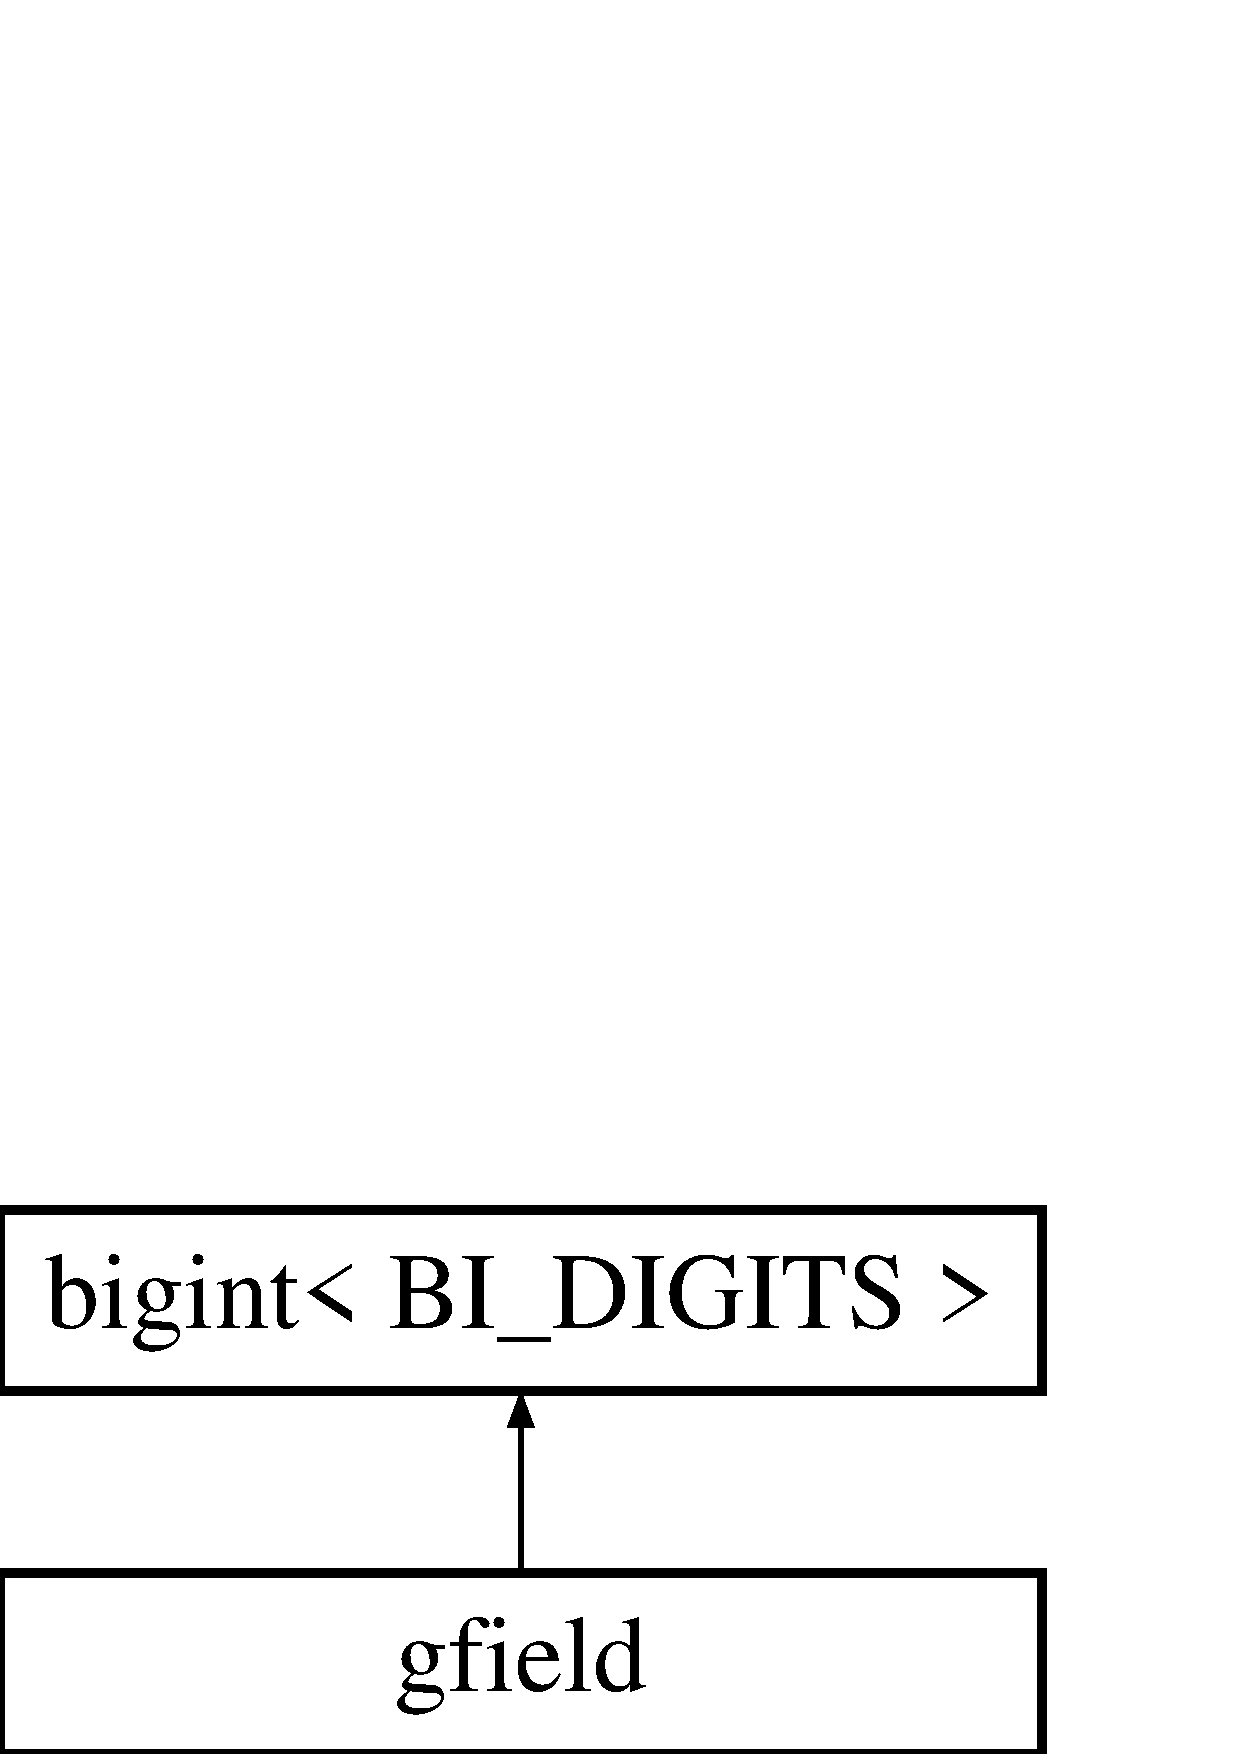
\includegraphics[height=2.000000cm]{structbigint}
\end{center}
\end{figure}
\subsection*{Public Types}
\begin{DoxyCompactItemize}
\item 
\mbox{\Hypertarget{structbigint_a4c2a0c25f7ff43453c16d96efa3d2726}\label{structbigint_a4c2a0c25f7ff43453c16d96efa3d2726}} 
typedef ushort {\bfseries digit}
\item 
\mbox{\Hypertarget{structbigint_a5731355b36cfe9d5292607ff58ba269b}\label{structbigint_a5731355b36cfe9d5292607ff58ba269b}} 
typedef uint {\bfseries dbldigit}
\end{DoxyCompactItemize}
\subsection*{Public Member Functions}
\begin{DoxyCompactItemize}
\item 
\mbox{\Hypertarget{structbigint_a8e74f28ee62ce0851f3b6d947463344f}\label{structbigint_a8e74f28ee62ce0851f3b6d947463344f}} 
{\bfseries bigint} (digit n)
\item 
\mbox{\Hypertarget{structbigint_a75949f03e408b5d1871a6a7122474442}\label{structbigint_a75949f03e408b5d1871a6a7122474442}} 
{\bfseries bigint} (const char $\ast$s)
\item 
\mbox{\Hypertarget{structbigint_a623f3e31d947e7bbf8dfe9984d0dc953}\label{structbigint_a623f3e31d947e7bbf8dfe9984d0dc953}} 
{\footnotesize template$<$int Y\+\_\+\+D\+I\+G\+I\+TS$>$ }\\{\bfseries bigint} (const \hyperlink{structbigint}{bigint}$<$ Y\+\_\+\+D\+I\+G\+I\+TS $>$ \&y)
\item 
\mbox{\Hypertarget{structbigint_a0634f5c2abbcaf7fab7fa4f7eb61f357}\label{structbigint_a0634f5c2abbcaf7fab7fa4f7eb61f357}} 
void {\bfseries parse} (const char $\ast$s)
\item 
\mbox{\Hypertarget{structbigint_af3f89b92f9f022f57deb3ec15908cc88}\label{structbigint_af3f89b92f9f022f57deb3ec15908cc88}} 
void {\bfseries zero} ()
\item 
\mbox{\Hypertarget{structbigint_ad32bde5f57a87ed21fc114d951d302f0}\label{structbigint_ad32bde5f57a87ed21fc114d951d302f0}} 
void {\bfseries print} (\hyperlink{structstream}{stream} $\ast$out) const
\item 
\mbox{\Hypertarget{structbigint_afe7caa5c899dfecf66337e338b109a8b}\label{structbigint_afe7caa5c899dfecf66337e338b109a8b}} 
void {\bfseries printdigits} (\hyperlink{structvector}{vector}$<$ char $>$ \&buf) const
\item 
\mbox{\Hypertarget{structbigint_a0e57759a6513e0b417eba2d14ce6498b}\label{structbigint_a0e57759a6513e0b417eba2d14ce6498b}} 
{\footnotesize template$<$int Y\+\_\+\+D\+I\+G\+I\+TS$>$ }\\\hyperlink{structbigint}{bigint} \& {\bfseries operator=} (const \hyperlink{structbigint}{bigint}$<$ Y\+\_\+\+D\+I\+G\+I\+TS $>$ \&y)
\item 
\mbox{\Hypertarget{structbigint_a69dabbaae951785466a48875e08be9af}\label{structbigint_a69dabbaae951785466a48875e08be9af}} 
bool {\bfseries iszero} () const
\item 
\mbox{\Hypertarget{structbigint_a9eab9fc59fd94f8864f872dcf43db5f6}\label{structbigint_a9eab9fc59fd94f8864f872dcf43db5f6}} 
bool {\bfseries isone} () const
\item 
\mbox{\Hypertarget{structbigint_a6b30764ad71fc751522c2d88e8f51469}\label{structbigint_a6b30764ad71fc751522c2d88e8f51469}} 
int {\bfseries numbits} () const
\item 
\mbox{\Hypertarget{structbigint_a8fc7a7e90cf0a50c0ad2154467622ca1}\label{structbigint_a8fc7a7e90cf0a50c0ad2154467622ca1}} 
bool {\bfseries hasbit} (int n) const
\item 
\mbox{\Hypertarget{structbigint_a1f5588d9e62942ef3ca83996fc09eda9}\label{structbigint_a1f5588d9e62942ef3ca83996fc09eda9}} 
bool {\bfseries morebits} (int n) const
\item 
\mbox{\Hypertarget{structbigint_a83de2e0a69faa39b852074a3c9f9c428}\label{structbigint_a83de2e0a69faa39b852074a3c9f9c428}} 
{\footnotesize template$<$int X\+\_\+\+D\+I\+G\+I\+TS, int Y\+\_\+\+D\+I\+G\+I\+TS$>$ }\\\hyperlink{structbigint}{bigint} \& {\bfseries add} (const \hyperlink{structbigint}{bigint}$<$ X\+\_\+\+D\+I\+G\+I\+TS $>$ \&x, const \hyperlink{structbigint}{bigint}$<$ Y\+\_\+\+D\+I\+G\+I\+TS $>$ \&y)
\item 
\mbox{\Hypertarget{structbigint_af39bc07861dec7beb1113f87c1210897}\label{structbigint_af39bc07861dec7beb1113f87c1210897}} 
{\footnotesize template$<$int Y\+\_\+\+D\+I\+G\+I\+TS$>$ }\\\hyperlink{structbigint}{bigint} \& {\bfseries add} (const \hyperlink{structbigint}{bigint}$<$ Y\+\_\+\+D\+I\+G\+I\+TS $>$ \&y)
\item 
\mbox{\Hypertarget{structbigint_a61d22457b7cefdcbc901c48ef4e0d6ac}\label{structbigint_a61d22457b7cefdcbc901c48ef4e0d6ac}} 
{\footnotesize template$<$int X\+\_\+\+D\+I\+G\+I\+TS, int Y\+\_\+\+D\+I\+G\+I\+TS$>$ }\\\hyperlink{structbigint}{bigint} \& {\bfseries sub} (const \hyperlink{structbigint}{bigint}$<$ X\+\_\+\+D\+I\+G\+I\+TS $>$ \&x, const \hyperlink{structbigint}{bigint}$<$ Y\+\_\+\+D\+I\+G\+I\+TS $>$ \&y)
\item 
\mbox{\Hypertarget{structbigint_ae78b03cf65e8dc3f83f295666db944d0}\label{structbigint_ae78b03cf65e8dc3f83f295666db944d0}} 
{\footnotesize template$<$int Y\+\_\+\+D\+I\+G\+I\+TS$>$ }\\\hyperlink{structbigint}{bigint} \& {\bfseries sub} (const \hyperlink{structbigint}{bigint}$<$ Y\+\_\+\+D\+I\+G\+I\+TS $>$ \&y)
\item 
\mbox{\Hypertarget{structbigint_a38a2d634b288f4c23f406bcb794de22b}\label{structbigint_a38a2d634b288f4c23f406bcb794de22b}} 
void {\bfseries shrink} ()
\item 
\mbox{\Hypertarget{structbigint_a1cc3b88393338ca9c1813d36b4636601}\label{structbigint_a1cc3b88393338ca9c1813d36b4636601}} 
void {\bfseries shrinkdigits} (int n)
\item 
\mbox{\Hypertarget{structbigint_a3498ee3a712c2057a900217ffc9e39fa}\label{structbigint_a3498ee3a712c2057a900217ffc9e39fa}} 
void {\bfseries shrinkbits} (int n)
\item 
\mbox{\Hypertarget{structbigint_a02338caddb7028e53afe0d463a1ad436}\label{structbigint_a02338caddb7028e53afe0d463a1ad436}} 
{\footnotesize template$<$int Y\+\_\+\+D\+I\+G\+I\+TS$>$ }\\void {\bfseries copyshrinkdigits} (const \hyperlink{structbigint}{bigint}$<$ Y\+\_\+\+D\+I\+G\+I\+TS $>$ \&y, int n)
\item 
\mbox{\Hypertarget{structbigint_a9cc3c9a99a3b52b9da27500514f22bfa}\label{structbigint_a9cc3c9a99a3b52b9da27500514f22bfa}} 
{\footnotesize template$<$int Y\+\_\+\+D\+I\+G\+I\+TS$>$ }\\void {\bfseries copyshrinkbits} (const \hyperlink{structbigint}{bigint}$<$ Y\+\_\+\+D\+I\+G\+I\+TS $>$ \&y, int n)
\item 
\mbox{\Hypertarget{structbigint_a916fbb1ce43a8dff864d90452890b91e}\label{structbigint_a916fbb1ce43a8dff864d90452890b91e}} 
{\footnotesize template$<$int X\+\_\+\+D\+I\+G\+I\+TS, int Y\+\_\+\+D\+I\+G\+I\+TS$>$ }\\\hyperlink{structbigint}{bigint} \& {\bfseries mul} (const \hyperlink{structbigint}{bigint}$<$ X\+\_\+\+D\+I\+G\+I\+TS $>$ \&x, const \hyperlink{structbigint}{bigint}$<$ Y\+\_\+\+D\+I\+G\+I\+TS $>$ \&y)
\item 
\mbox{\Hypertarget{structbigint_a0a11867c8ff9b0f2ab796fe25b5f4733}\label{structbigint_a0a11867c8ff9b0f2ab796fe25b5f4733}} 
\hyperlink{structbigint}{bigint} \& {\bfseries rshift} (int n)
\item 
\mbox{\Hypertarget{structbigint_a160aacfae19cfa773b89a1fb3c8b033f}\label{structbigint_a160aacfae19cfa773b89a1fb3c8b033f}} 
\hyperlink{structbigint}{bigint} \& {\bfseries lshift} (int n)
\item 
\mbox{\Hypertarget{structbigint_ae14cecc50be88164a6b84456cbd0d600}\label{structbigint_ae14cecc50be88164a6b84456cbd0d600}} 
void {\bfseries zerodigits} (int i, int n)
\item 
\mbox{\Hypertarget{structbigint_a97bf226c66e0b6ed908910997f7c4461}\label{structbigint_a97bf226c66e0b6ed908910997f7c4461}} 
void {\bfseries zerobits} (int i, int n)
\item 
\mbox{\Hypertarget{structbigint_a4694155d250bbc896ddce4d294681c8f}\label{structbigint_a4694155d250bbc896ddce4d294681c8f}} 
{\footnotesize template$<$int Y\+\_\+\+D\+I\+G\+I\+TS$>$ }\\void {\bfseries copydigits} (int to, const \hyperlink{structbigint}{bigint}$<$ Y\+\_\+\+D\+I\+G\+I\+TS $>$ \&y, int from, int n)
\item 
\mbox{\Hypertarget{structbigint_a262bca28b013b25af643bb691af40a3a}\label{structbigint_a262bca28b013b25af643bb691af40a3a}} 
{\footnotesize template$<$int Y\+\_\+\+D\+I\+G\+I\+TS$>$ }\\void {\bfseries copybits} (int to, const \hyperlink{structbigint}{bigint}$<$ Y\+\_\+\+D\+I\+G\+I\+TS $>$ \&y, int from, int n)
\item 
\mbox{\Hypertarget{structbigint_a5d12ed3c4a08d3ccbb318d9c5fb906ce}\label{structbigint_a5d12ed3c4a08d3ccbb318d9c5fb906ce}} 
void {\bfseries dupdigits} (int to, int from, int n)
\item 
\mbox{\Hypertarget{structbigint_aa74fdf7e468f16bf49383ef8083e5e62}\label{structbigint_aa74fdf7e468f16bf49383ef8083e5e62}} 
void {\bfseries dupbits} (int to, int from, int n)
\item 
\mbox{\Hypertarget{structbigint_a52ae643a11c12fde1df268428ecae7cd}\label{structbigint_a52ae643a11c12fde1df268428ecae7cd}} 
{\footnotesize template$<$int Y\+\_\+\+D\+I\+G\+I\+TS$>$ }\\bool {\bfseries operator==} (const \hyperlink{structbigint}{bigint}$<$ Y\+\_\+\+D\+I\+G\+I\+TS $>$ \&y) const
\item 
\mbox{\Hypertarget{structbigint_aa1a4b8f666b091218a239487babfb05e}\label{structbigint_aa1a4b8f666b091218a239487babfb05e}} 
{\footnotesize template$<$int Y\+\_\+\+D\+I\+G\+I\+TS$>$ }\\bool {\bfseries operator!=} (const \hyperlink{structbigint}{bigint}$<$ Y\+\_\+\+D\+I\+G\+I\+TS $>$ \&y) const
\item 
\mbox{\Hypertarget{structbigint_adde64ef4f3e9c35e7d520a731108aba4}\label{structbigint_adde64ef4f3e9c35e7d520a731108aba4}} 
{\footnotesize template$<$int Y\+\_\+\+D\+I\+G\+I\+TS$>$ }\\bool {\bfseries operator$<$} (const \hyperlink{structbigint}{bigint}$<$ Y\+\_\+\+D\+I\+G\+I\+TS $>$ \&y) const
\item 
\mbox{\Hypertarget{structbigint_ac9a645a1bca2713954e5fc12a9712f30}\label{structbigint_ac9a645a1bca2713954e5fc12a9712f30}} 
{\footnotesize template$<$int Y\+\_\+\+D\+I\+G\+I\+TS$>$ }\\bool {\bfseries operator$>$} (const \hyperlink{structbigint}{bigint}$<$ Y\+\_\+\+D\+I\+G\+I\+TS $>$ \&y) const
\item 
\mbox{\Hypertarget{structbigint_ae3eea80018ba3c4348586b412be3674f}\label{structbigint_ae3eea80018ba3c4348586b412be3674f}} 
{\footnotesize template$<$int Y\+\_\+\+D\+I\+G\+I\+TS$>$ }\\bool {\bfseries operator$<$=} (const \hyperlink{structbigint}{bigint}$<$ Y\+\_\+\+D\+I\+G\+I\+TS $>$ \&y) const
\item 
\mbox{\Hypertarget{structbigint_a638bc743bb86d6df3d0f30ad5b771685}\label{structbigint_a638bc743bb86d6df3d0f30ad5b771685}} 
{\footnotesize template$<$int Y\+\_\+\+D\+I\+G\+I\+TS$>$ }\\bool {\bfseries operator$>$=} (const \hyperlink{structbigint}{bigint}$<$ Y\+\_\+\+D\+I\+G\+I\+TS $>$ \&y) const
\end{DoxyCompactItemize}
\subsection*{Static Public Member Functions}
\begin{DoxyCompactItemize}
\item 
\mbox{\Hypertarget{structbigint_aa307c43dfccd4ecf23aaa4533635eb4a}\label{structbigint_aa307c43dfccd4ecf23aaa4533635eb4a}} 
static int {\bfseries parsedigits} (ushort $\ast$digits, int maxlen, const char $\ast$s)
\end{DoxyCompactItemize}
\subsection*{Public Attributes}
\begin{DoxyCompactItemize}
\item 
\mbox{\Hypertarget{structbigint_af00912d392799078ac8eb452a3b04d5a}\label{structbigint_af00912d392799078ac8eb452a3b04d5a}} 
int {\bfseries len}
\item 
\mbox{\Hypertarget{structbigint_a0e5b25c406c20d6156f12bfd3f7e8596}\label{structbigint_a0e5b25c406c20d6156f12bfd3f7e8596}} 
digit {\bfseries digits} \mbox{[}B\+I\+\_\+\+D\+I\+G\+I\+TS\mbox{]}
\end{DoxyCompactItemize}


The documentation for this struct was generated from the following file\+:\begin{DoxyCompactItemize}
\item 
H\+:/\+Rival\+Engine/\+Rival\+\_\+\+Game\+\_\+\+Engine\+\_\+\+G\+I\+T/\+Rival3dengine/source/shared/crypto.\+cpp\end{DoxyCompactItemize}

\hypertarget{struct_b_i_h}{}\section{B\+IH Struct Reference}
\label{struct_b_i_h}\index{B\+IH@{B\+IH}}
\subsection*{Classes}
\begin{DoxyCompactItemize}
\item 
struct \hyperlink{struct_b_i_h_1_1mesh}{mesh}
\item 
struct \hyperlink{struct_b_i_h_1_1node}{node}
\item 
struct \hyperlink{struct_b_i_h_1_1tri}{tri}
\item 
struct \hyperlink{struct_b_i_h_1_1tribb}{tribb}
\end{DoxyCompactItemize}
\subsection*{Public Types}
\begin{DoxyCompactItemize}
\item 
\mbox{\Hypertarget{struct_b_i_h_ace901662594827aaf93ac979468a34e3}\label{struct_b_i_h_ace901662594827aaf93ac979468a34e3}} 
enum \{ {\bfseries M\+E\+S\+H\+\_\+\+R\+E\+N\+D\+ER} = 1$<$$<$1, 
{\bfseries M\+E\+S\+H\+\_\+\+N\+O\+C\+L\+IP} = 1$<$$<$2, 
{\bfseries M\+E\+S\+H\+\_\+\+A\+L\+P\+HA} = 1$<$$<$3, 
{\bfseries M\+E\+S\+H\+\_\+\+C\+O\+L\+L\+I\+DE} = 1$<$$<$4
 \}
\end{DoxyCompactItemize}
\subsection*{Public Member Functions}
\begin{DoxyCompactItemize}
\item 
\mbox{\Hypertarget{struct_b_i_h_a4a1d96504f62de65d81e6c06fad6df95}\label{struct_b_i_h_a4a1d96504f62de65d81e6c06fad6df95}} 
{\bfseries B\+IH} (\hyperlink{structvector}{vector}$<$ \hyperlink{struct_b_i_h_1_1mesh}{mesh} $>$ \&buildmeshes)
\item 
\mbox{\Hypertarget{struct_b_i_h_a8d450c6727f42ead5aa3109dc93fb769}\label{struct_b_i_h_a8d450c6727f42ead5aa3109dc93fb769}} 
void {\bfseries build} (\hyperlink{struct_b_i_h_1_1mesh}{mesh} \&m, ushort $\ast$indices, int numindices, const \hyperlink{structivec}{ivec} \&vmin, const \hyperlink{structivec}{ivec} \&vmax)
\item 
\mbox{\Hypertarget{struct_b_i_h_ac662df92c82507c40746c423f47f1cdc}\label{struct_b_i_h_ac662df92c82507c40746c423f47f1cdc}} 
bool {\bfseries traverse} (const \hyperlink{structvec}{vec} \&o, const \hyperlink{structvec}{vec} \&ray, float maxdist, float \&dist, int mode)
\item 
\mbox{\Hypertarget{struct_b_i_h_aec96572a18eef6013c9af964bc1a18f6}\label{struct_b_i_h_aec96572a18eef6013c9af964bc1a18f6}} 
bool {\bfseries traverse} (const \hyperlink{struct_b_i_h_1_1mesh}{mesh} \&m, const \hyperlink{structvec}{vec} \&o, const \hyperlink{structvec}{vec} \&ray, const \hyperlink{structvec}{vec} \&invray, float maxdist, float \&dist, int mode, \hyperlink{struct_b_i_h_1_1node}{node} $\ast$curnode, float tmin, float tmax)
\item 
\mbox{\Hypertarget{struct_b_i_h_ad0e3bb00b361092705b7f88fe7bc762d}\label{struct_b_i_h_ad0e3bb00b361092705b7f88fe7bc762d}} 
bool {\bfseries triintersect} (const \hyperlink{struct_b_i_h_1_1mesh}{mesh} \&m, int tidx, const \hyperlink{structvec}{vec} \&mo, const \hyperlink{structvec}{vec} \&mray, float maxdist, float \&dist, int mode)
\item 
\mbox{\Hypertarget{struct_b_i_h_ace158c17b8c16818edb053f1a673a7ce}\label{struct_b_i_h_ace158c17b8c16818edb053f1a673a7ce}} 
bool {\bfseries boxcollide} (\hyperlink{structphysent}{physent} $\ast$d, const \hyperlink{structvec}{vec} \&dir, float cutoff, const \hyperlink{structvec}{vec} \&o, int yaw, int pitch, int roll, float scale=1)
\item 
\mbox{\Hypertarget{struct_b_i_h_a1ebb0933334624cc462e82afbd2d138e}\label{struct_b_i_h_a1ebb0933334624cc462e82afbd2d138e}} 
bool {\bfseries ellipsecollide} (\hyperlink{structphysent}{physent} $\ast$d, const \hyperlink{structvec}{vec} \&dir, float cutoff, const \hyperlink{structvec}{vec} \&o, int yaw, int pitch, int roll, float scale=1)
\item 
\mbox{\Hypertarget{struct_b_i_h_a99c9594d69e05f8a3573a68e7beb042b}\label{struct_b_i_h_a99c9594d69e05f8a3573a68e7beb042b}} 
{\footnotesize template$<$int C$>$ }\\void {\bfseries collide} (const \hyperlink{struct_b_i_h_1_1mesh}{mesh} \&m, \hyperlink{structphysent}{physent} $\ast$d, const \hyperlink{structvec}{vec} \&dir, float cutoff, const \hyperlink{structvec}{vec} \&center, const \hyperlink{structvec}{vec} \&radius, const \hyperlink{structmatrix4x3}{matrix4x3} \&orient, float \&dist, \hyperlink{struct_b_i_h_1_1node}{node} $\ast$curnode, const \hyperlink{structivec}{ivec} \&bo, const \hyperlink{structivec}{ivec} \&br)
\item 
\mbox{\Hypertarget{struct_b_i_h_a7ece631d54709a1994c72cfa10431a24}\label{struct_b_i_h_a7ece631d54709a1994c72cfa10431a24}} 
{\footnotesize template$<$int C$>$ }\\void {\bfseries tricollide} (const \hyperlink{struct_b_i_h_1_1mesh}{mesh} \&m, int tidx, \hyperlink{structphysent}{physent} $\ast$d, const \hyperlink{structvec}{vec} \&dir, float cutoff, const \hyperlink{structvec}{vec} \&center, const \hyperlink{structvec}{vec} \&radius, const \hyperlink{structmatrix4x3}{matrix4x3} \&orient, float \&dist, const \hyperlink{structivec}{ivec} \&bo, const \hyperlink{structivec}{ivec} \&br)
\item 
\mbox{\Hypertarget{struct_b_i_h_a69f1ea447e1bc18744a61e09f270c268}\label{struct_b_i_h_a69f1ea447e1bc18744a61e09f270c268}} 
void {\bfseries genstaintris} (\hyperlink{structstainrenderer}{stainrenderer} $\ast$s, const \hyperlink{structvec}{vec} \&staincenter, float stainradius, const \hyperlink{structvec}{vec} \&o, int yaw, int pitch, int roll, float scale=1)
\item 
\mbox{\Hypertarget{struct_b_i_h_a1b1edd7f4c38ea2be0c5ab8135d2284b}\label{struct_b_i_h_a1b1edd7f4c38ea2be0c5ab8135d2284b}} 
void {\bfseries genstaintris} (\hyperlink{structstainrenderer}{stainrenderer} $\ast$s, const \hyperlink{struct_b_i_h_1_1mesh}{mesh} \&m, const \hyperlink{structvec}{vec} \&center, float radius, const \hyperlink{structmatrix4x3}{matrix4x3} \&orient, \hyperlink{struct_b_i_h_1_1node}{node} $\ast$curnode, const \hyperlink{structivec}{ivec} \&bo, const \hyperlink{structivec}{ivec} \&br)
\item 
\mbox{\Hypertarget{struct_b_i_h_a2038d591a806f7a5e32975d8707a94ab}\label{struct_b_i_h_a2038d591a806f7a5e32975d8707a94ab}} 
void {\bfseries genstaintris} (\hyperlink{structstainrenderer}{stainrenderer} $\ast$s, const \hyperlink{struct_b_i_h_1_1mesh}{mesh} \&m, int tidx, const \hyperlink{structvec}{vec} \&center, float radius, const \hyperlink{structmatrix4x3}{matrix4x3} \&orient, const \hyperlink{structivec}{ivec} \&bo, const \hyperlink{structivec}{ivec} \&br)
\item 
\mbox{\Hypertarget{struct_b_i_h_ab4509d45d115644cb8377436ba1d6be1}\label{struct_b_i_h_ab4509d45d115644cb8377436ba1d6be1}} 
void {\bfseries preload} ()
\item 
\mbox{\Hypertarget{struct_b_i_h_a7847cf9ec6ac5fc60e5b12024e4a77c9}\label{struct_b_i_h_a7847cf9ec6ac5fc60e5b12024e4a77c9}} 
{\footnotesize template$<$$>$ }\\void {\bfseries tricollide} (const \hyperlink{struct_b_i_h_1_1mesh}{mesh} \&m, int tidx, \hyperlink{structphysent}{physent} $\ast$d, const \hyperlink{structvec}{vec} \&dir, float cutoff, const \hyperlink{structvec}{vec} \&center, const \hyperlink{structvec}{vec} \&radius, const \hyperlink{structmatrix4x3}{matrix4x3} \&orient, float \&dist, const \hyperlink{structivec}{ivec} \&bo, const \hyperlink{structivec}{ivec} \&br)
\item 
\mbox{\Hypertarget{struct_b_i_h_a7847cf9ec6ac5fc60e5b12024e4a77c9}\label{struct_b_i_h_a7847cf9ec6ac5fc60e5b12024e4a77c9}} 
{\footnotesize template$<$$>$ }\\void {\bfseries tricollide} (const \hyperlink{struct_b_i_h_1_1mesh}{mesh} \&m, int tidx, \hyperlink{structphysent}{physent} $\ast$d, const \hyperlink{structvec}{vec} \&dir, float cutoff, const \hyperlink{structvec}{vec} \&center, const \hyperlink{structvec}{vec} \&radius, const \hyperlink{structmatrix4x3}{matrix4x3} \&orient, float \&dist, const \hyperlink{structivec}{ivec} \&bo, const \hyperlink{structivec}{ivec} \&br)
\end{DoxyCompactItemize}
\subsection*{Public Attributes}
\begin{DoxyCompactItemize}
\item 
\mbox{\Hypertarget{struct_b_i_h_a596b4f2699831b227c7ef39a507f11f8}\label{struct_b_i_h_a596b4f2699831b227c7ef39a507f11f8}} 
\hyperlink{struct_b_i_h_1_1mesh}{mesh} $\ast$ {\bfseries meshes}
\item 
\mbox{\Hypertarget{struct_b_i_h_a7ba639f2f3f4c580390b279a07b8593d}\label{struct_b_i_h_a7ba639f2f3f4c580390b279a07b8593d}} 
int {\bfseries nummeshes}
\item 
\mbox{\Hypertarget{struct_b_i_h_a95b4c328b2098e2070e85b120985b528}\label{struct_b_i_h_a95b4c328b2098e2070e85b120985b528}} 
\hyperlink{struct_b_i_h_1_1node}{node} $\ast$ {\bfseries nodes}
\item 
\mbox{\Hypertarget{struct_b_i_h_ae10f080c7fd742588e31fc5d3426cbb4}\label{struct_b_i_h_ae10f080c7fd742588e31fc5d3426cbb4}} 
int {\bfseries numnodes}
\item 
\mbox{\Hypertarget{struct_b_i_h_a0c6316bde35c73d4ed0eae5f304f92de}\label{struct_b_i_h_a0c6316bde35c73d4ed0eae5f304f92de}} 
\hyperlink{struct_b_i_h_1_1tribb}{tribb} $\ast$ {\bfseries tribbs}
\item 
\mbox{\Hypertarget{struct_b_i_h_adde0b38c1a8ad466748b56a77b5c85d2}\label{struct_b_i_h_adde0b38c1a8ad466748b56a77b5c85d2}} 
int {\bfseries numtris}
\item 
\mbox{\Hypertarget{struct_b_i_h_afa88ff782bc1d97d9856a2443c6d8c77}\label{struct_b_i_h_afa88ff782bc1d97d9856a2443c6d8c77}} 
\hyperlink{structvec}{vec} {\bfseries bbmin}
\item 
\mbox{\Hypertarget{struct_b_i_h_aacd20a7c1cb09e747f1ee69c622f0985}\label{struct_b_i_h_aacd20a7c1cb09e747f1ee69c622f0985}} 
\hyperlink{structvec}{vec} {\bfseries bbmax}
\item 
\mbox{\Hypertarget{struct_b_i_h_a22a3b36b8081d49228fc56a2e6db3ccc}\label{struct_b_i_h_a22a3b36b8081d49228fc56a2e6db3ccc}} 
\hyperlink{structvec}{vec} {\bfseries center}
\item 
\mbox{\Hypertarget{struct_b_i_h_ad7870a81de3301279043cc49268d46cd}\label{struct_b_i_h_ad7870a81de3301279043cc49268d46cd}} 
float {\bfseries radius}
\item 
\mbox{\Hypertarget{struct_b_i_h_a533795f5b43acf8c567a2552447826f6}\label{struct_b_i_h_a533795f5b43acf8c567a2552447826f6}} 
float {\bfseries entradius}
\end{DoxyCompactItemize}


The documentation for this struct was generated from the following files\+:\begin{DoxyCompactItemize}
\item 
H\+:/\+Rival\+Engine/\+Rival\+\_\+\+Game\+\_\+\+Engine\+\_\+\+G\+I\+T/\+Rival3dengine/source/engine/bih.\+h\item 
H\+:/\+Rival\+Engine/\+Rival\+\_\+\+Game\+\_\+\+Engine\+\_\+\+G\+I\+T/\+Rival3dengine/source/engine/bih.\+cpp\end{DoxyCompactItemize}

\hypertarget{struct_blend_brush}{}\section{Blend\+Brush Struct Reference}
\label{struct_blend_brush}\index{Blend\+Brush@{Blend\+Brush}}
\subsection*{Public Member Functions}
\begin{DoxyCompactItemize}
\item 
\mbox{\Hypertarget{struct_blend_brush_aeccea22b6666eea32274b19ae153e3ac}\label{struct_blend_brush_aeccea22b6666eea32274b19ae153e3ac}} 
{\bfseries Blend\+Brush} (const char $\ast$name, int w, int h)
\item 
\mbox{\Hypertarget{struct_blend_brush_a624cfc96604bd8b55dc7b2cd361abc9d}\label{struct_blend_brush_a624cfc96604bd8b55dc7b2cd361abc9d}} 
void {\bfseries cleanup} ()
\item 
\mbox{\Hypertarget{struct_blend_brush_ac08b909c75e550e00ad10286e8275f63}\label{struct_blend_brush_ac08b909c75e550e00ad10286e8275f63}} 
void {\bfseries gentex} ()
\item 
\mbox{\Hypertarget{struct_blend_brush_a7fdb5920031439de12467f22f4d8ed00}\label{struct_blend_brush_a7fdb5920031439de12467f22f4d8ed00}} 
void {\bfseries reorient} (bool flipx, bool flipy, bool swapxy)
\end{DoxyCompactItemize}
\subsection*{Public Attributes}
\begin{DoxyCompactItemize}
\item 
\mbox{\Hypertarget{struct_blend_brush_a0d842754e6d87186d7c3d6a70c0fa102}\label{struct_blend_brush_a0d842754e6d87186d7c3d6a70c0fa102}} 
char $\ast$ {\bfseries name}
\item 
\mbox{\Hypertarget{struct_blend_brush_aa90e98fa4d3f170cde6c70bc0a9a8600}\label{struct_blend_brush_aa90e98fa4d3f170cde6c70bc0a9a8600}} 
int {\bfseries w}
\item 
\mbox{\Hypertarget{struct_blend_brush_a553d616391886a7e8dca942cf635182e}\label{struct_blend_brush_a553d616391886a7e8dca942cf635182e}} 
int {\bfseries h}
\item 
\mbox{\Hypertarget{struct_blend_brush_a3041abd5b7821e3145e07138286c54d2}\label{struct_blend_brush_a3041abd5b7821e3145e07138286c54d2}} 
uchar $\ast$ {\bfseries data}
\item 
\mbox{\Hypertarget{struct_blend_brush_a075aaaa419bd11d6b5754f43fe88fe86}\label{struct_blend_brush_a075aaaa419bd11d6b5754f43fe88fe86}} 
G\+Luint {\bfseries tex}
\end{DoxyCompactItemize}


The documentation for this struct was generated from the following file\+:\begin{DoxyCompactItemize}
\item 
H\+:/\+Rival\+Engine/\+Rival\+\_\+\+Game\+\_\+\+Engine\+\_\+\+G\+I\+T/\+Rival3dengine/source/engine/blend.\+cpp\end{DoxyCompactItemize}

\hypertarget{structskelmodel_1_1blendcacheentry}{}\section{skelmodel\+:\+:blendcacheentry Struct Reference}
\label{structskelmodel_1_1blendcacheentry}\index{skelmodel\+::blendcacheentry@{skelmodel\+::blendcacheentry}}
Inheritance diagram for skelmodel\+:\+:blendcacheentry\+:\begin{figure}[H]
\begin{center}
\leavevmode
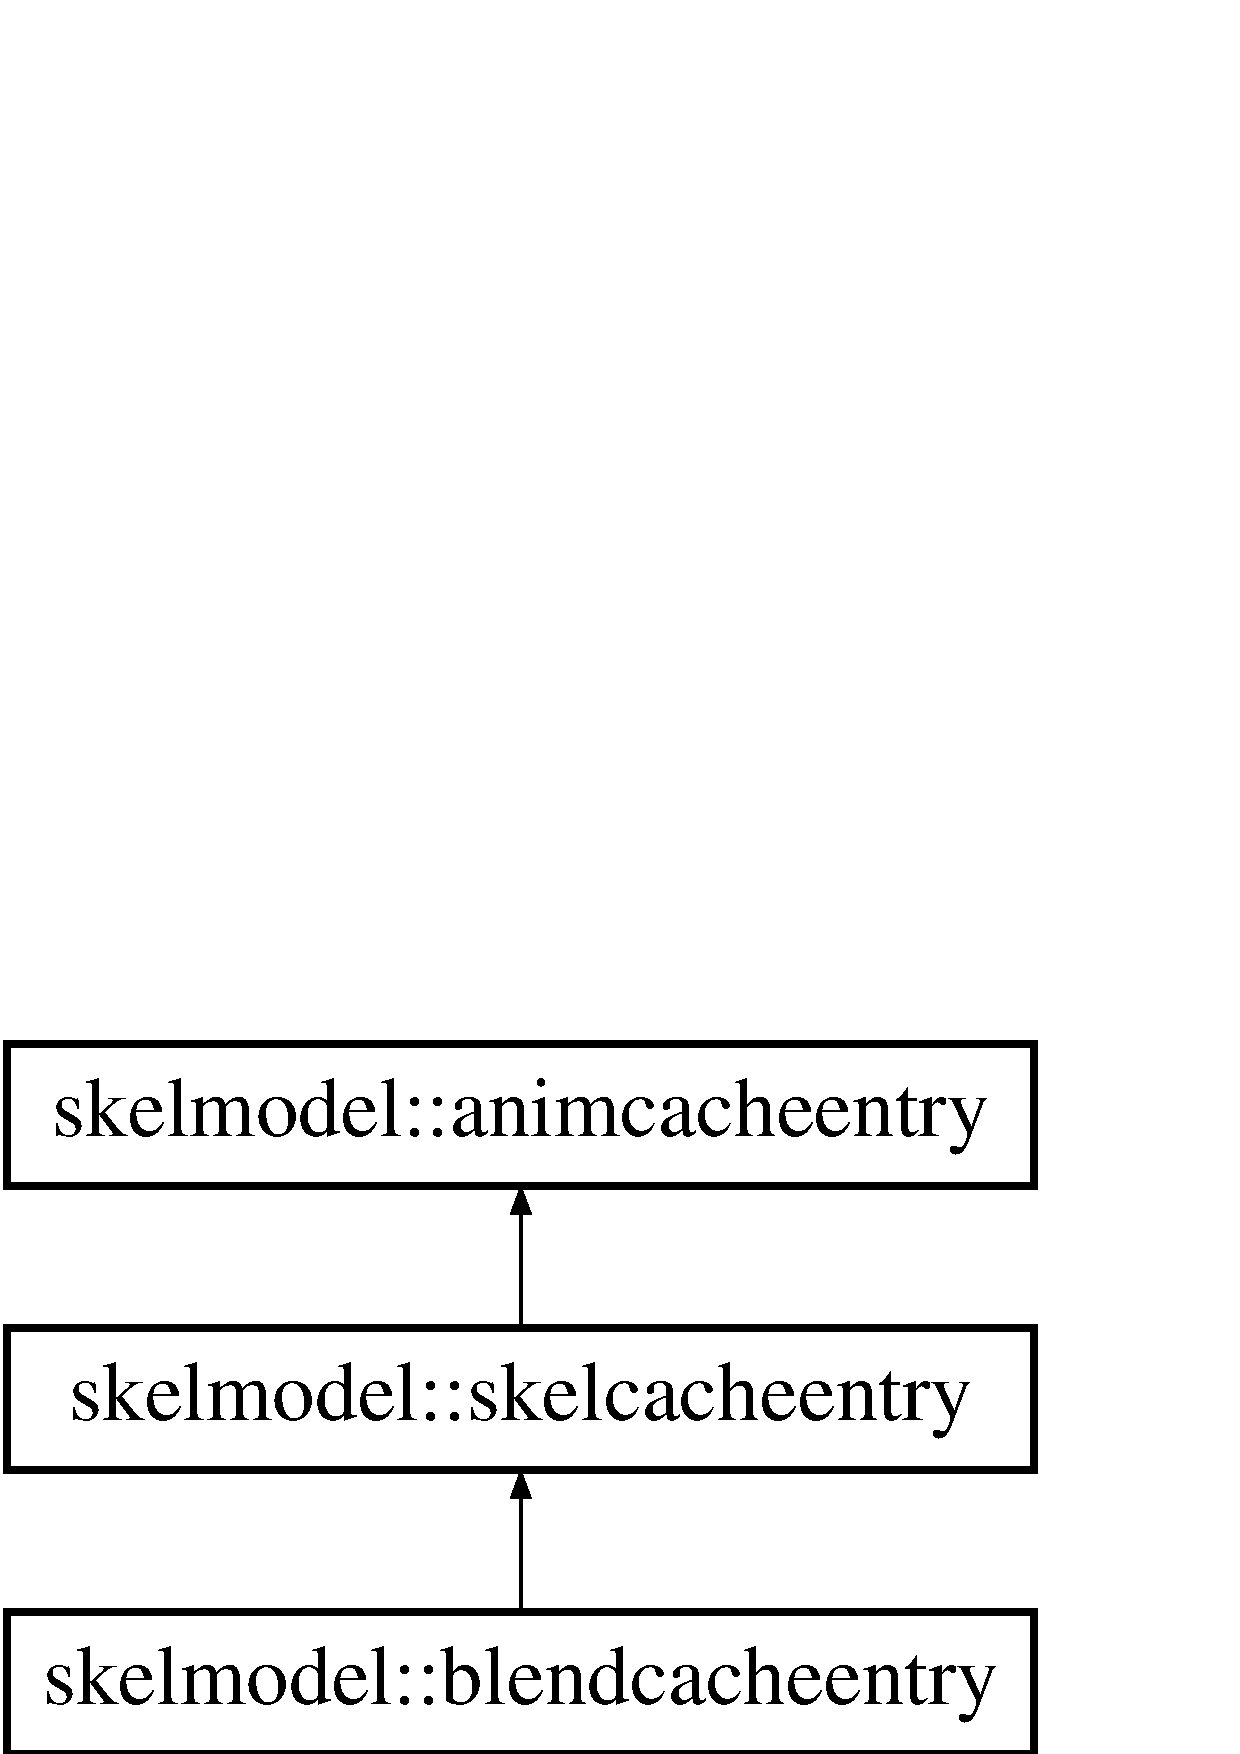
\includegraphics[height=3.000000cm]{structskelmodel_1_1blendcacheentry}
\end{center}
\end{figure}
\subsection*{Public Attributes}
\begin{DoxyCompactItemize}
\item 
\mbox{\Hypertarget{structskelmodel_1_1blendcacheentry_a1996b49797c1a0b01985abbcdcdca2c7}\label{structskelmodel_1_1blendcacheentry_a1996b49797c1a0b01985abbcdcdca2c7}} 
int {\bfseries owner}
\end{DoxyCompactItemize}
\subsection*{Additional Inherited Members}


The documentation for this struct was generated from the following file\+:\begin{DoxyCompactItemize}
\item 
H\+:/\+Rival\+Engine/\+Rival\+\_\+\+Game\+\_\+\+Engine\+\_\+\+G\+I\+T/\+Rival3dengine/source/engine/skelmodel.\+h\end{DoxyCompactItemize}

\hypertarget{structskelmodel_1_1blendcombo}{}\section{skelmodel\+:\+:blendcombo Struct Reference}
\label{structskelmodel_1_1blendcombo}\index{skelmodel\+::blendcombo@{skelmodel\+::blendcombo}}
\subsection*{Public Member Functions}
\begin{DoxyCompactItemize}
\item 
\mbox{\Hypertarget{structskelmodel_1_1blendcombo_a7b0384dfb361effb7583bd7ce4a1d386}\label{structskelmodel_1_1blendcombo_a7b0384dfb361effb7583bd7ce4a1d386}} 
bool {\bfseries operator==} (const \hyperlink{structskelmodel_1_1blendcombo}{blendcombo} \&c) const
\item 
\mbox{\Hypertarget{structskelmodel_1_1blendcombo_ae07369bfe9fa0d4b547530ed3a7b2b1d}\label{structskelmodel_1_1blendcombo_ae07369bfe9fa0d4b547530ed3a7b2b1d}} 
int {\bfseries size} () const
\item 
\mbox{\Hypertarget{structskelmodel_1_1blendcombo_a75c55f2ecf9fd744dd3126fd50ae8537}\label{structskelmodel_1_1blendcombo_a75c55f2ecf9fd744dd3126fd50ae8537}} 
int {\bfseries addweight} (int sorted, float weight, int bone)
\item 
\mbox{\Hypertarget{structskelmodel_1_1blendcombo_a18da71f5729c63cbd1599731ebba038c}\label{structskelmodel_1_1blendcombo_a18da71f5729c63cbd1599731ebba038c}} 
void {\bfseries finalize} (int sorted)
\item 
\mbox{\Hypertarget{structskelmodel_1_1blendcombo_a3defb7b60da7b5c2f76997678f51e5e4}\label{structskelmodel_1_1blendcombo_a3defb7b60da7b5c2f76997678f51e5e4}} 
{\footnotesize template$<$class T $>$ }\\void {\bfseries serialize} (T \&v)
\end{DoxyCompactItemize}
\subsection*{Static Public Member Functions}
\begin{DoxyCompactItemize}
\item 
\mbox{\Hypertarget{structskelmodel_1_1blendcombo_a6a56dd18955aefd8efbb562d506bca06}\label{structskelmodel_1_1blendcombo_a6a56dd18955aefd8efbb562d506bca06}} 
static bool {\bfseries sortcmp} (const \hyperlink{structskelmodel_1_1blendcombo}{blendcombo} \&x, const \hyperlink{structskelmodel_1_1blendcombo}{blendcombo} \&y)
\end{DoxyCompactItemize}
\subsection*{Public Attributes}
\begin{DoxyCompactItemize}
\item 
\mbox{\Hypertarget{structskelmodel_1_1blendcombo_ac4e97850417feaa328277c3535fcb58e}\label{structskelmodel_1_1blendcombo_ac4e97850417feaa328277c3535fcb58e}} 
int {\bfseries uses}
\item 
\mbox{\Hypertarget{structskelmodel_1_1blendcombo_a7a92c3fcff480eb62aae93a38f3afd1f}\label{structskelmodel_1_1blendcombo_a7a92c3fcff480eb62aae93a38f3afd1f}} 
int {\bfseries interpindex}
\item 
\mbox{\Hypertarget{structskelmodel_1_1blendcombo_aca020de4c86cca6008ea0cc52c7b89f4}\label{structskelmodel_1_1blendcombo_aca020de4c86cca6008ea0cc52c7b89f4}} 
float {\bfseries weights} \mbox{[}4\mbox{]}
\item 
\mbox{\Hypertarget{structskelmodel_1_1blendcombo_af05ad0da556e0c9ea45ef6b74748ee20}\label{structskelmodel_1_1blendcombo_af05ad0da556e0c9ea45ef6b74748ee20}} 
uchar {\bfseries bones} \mbox{[}4\mbox{]}
\item 
\mbox{\Hypertarget{structskelmodel_1_1blendcombo_a87ead1cb42a59f214417e13697f33552}\label{structskelmodel_1_1blendcombo_a87ead1cb42a59f214417e13697f33552}} 
uchar {\bfseries interpbones} \mbox{[}4\mbox{]}
\end{DoxyCompactItemize}


The documentation for this struct was generated from the following file\+:\begin{DoxyCompactItemize}
\item 
H\+:/\+Rival\+Engine/\+Rival\+\_\+\+Game\+\_\+\+Engine\+\_\+\+G\+I\+T/\+Rival3dengine/source/engine/skelmodel.\+h\end{DoxyCompactItemize}

\hypertarget{struct_blend_map_branch}{}\section{Blend\+Map\+Branch Struct Reference}
\label{struct_blend_map_branch}\index{Blend\+Map\+Branch@{Blend\+Map\+Branch}}
\subsection*{Public Member Functions}
\begin{DoxyCompactItemize}
\item 
\mbox{\Hypertarget{struct_blend_map_branch_a75f4b2252539a7d66896ecec864f5d8d}\label{struct_blend_map_branch_a75f4b2252539a7d66896ecec864f5d8d}} 
uchar {\bfseries shrink} (\hyperlink{struct_blend_map_node}{Blend\+Map\+Node} \&child, int quadrant)
\end{DoxyCompactItemize}
\subsection*{Public Attributes}
\begin{DoxyCompactItemize}
\item 
\mbox{\Hypertarget{struct_blend_map_branch_a93c415f30e5049732ca8eea9b0b1d60b}\label{struct_blend_map_branch_a93c415f30e5049732ca8eea9b0b1d60b}} 
uchar {\bfseries type} \mbox{[}4\mbox{]}
\item 
\mbox{\Hypertarget{struct_blend_map_branch_af04ac5df68c681d57889e09b2518bf4b}\label{struct_blend_map_branch_af04ac5df68c681d57889e09b2518bf4b}} 
\hyperlink{struct_blend_map_node}{Blend\+Map\+Node} {\bfseries children} \mbox{[}4\mbox{]}
\end{DoxyCompactItemize}


The documentation for this struct was generated from the following file\+:\begin{DoxyCompactItemize}
\item 
H\+:/\+Rival\+Engine/\+Rival\+\_\+\+Game\+\_\+\+Engine\+\_\+\+G\+I\+T/\+Rival3dengine/source/engine/blend.\+cpp\end{DoxyCompactItemize}

\hypertarget{struct_blend_map_cache}{}\section{Blend\+Map\+Cache Struct Reference}
\label{struct_blend_map_cache}\index{Blend\+Map\+Cache@{Blend\+Map\+Cache}}
\subsection*{Public Attributes}
\begin{DoxyCompactItemize}
\item 
\mbox{\Hypertarget{struct_blend_map_cache_a9df8201d08307470db49b0ad1d038a4f}\label{struct_blend_map_cache_a9df8201d08307470db49b0ad1d038a4f}} 
\hyperlink{struct_blend_map_root}{Blend\+Map\+Root} {\bfseries node}
\item 
\mbox{\Hypertarget{struct_blend_map_cache_a51c90afa2edd8ff7a4868aa525a8f236}\label{struct_blend_map_cache_a51c90afa2edd8ff7a4868aa525a8f236}} 
int {\bfseries scale}
\item 
\mbox{\Hypertarget{struct_blend_map_cache_aa8145f41971c931cafd0df607cd273d2}\label{struct_blend_map_cache_aa8145f41971c931cafd0df607cd273d2}} 
\hyperlink{structivec2}{ivec2} {\bfseries origin}
\end{DoxyCompactItemize}


The documentation for this struct was generated from the following file\+:\begin{DoxyCompactItemize}
\item 
H\+:/\+Rival\+Engine/\+Rival\+\_\+\+Game\+\_\+\+Engine\+\_\+\+G\+I\+T/\+Rival3dengine/source/engine/blend.\+cpp\end{DoxyCompactItemize}

\hypertarget{struct_blend_map_image}{}\section{Blend\+Map\+Image Struct Reference}
\label{struct_blend_map_image}\index{Blend\+Map\+Image@{Blend\+Map\+Image}}
\subsection*{Public Attributes}
\begin{DoxyCompactItemize}
\item 
\mbox{\Hypertarget{struct_blend_map_image_a1d29a6cb308d710af5a80c1942304367}\label{struct_blend_map_image_a1d29a6cb308d710af5a80c1942304367}} 
uchar {\bfseries data} \mbox{[}B\+M\+\_\+\+I\+M\+A\+G\+E\+\_\+\+S\+I\+ZE $\ast$B\+M\+\_\+\+I\+M\+A\+G\+E\+\_\+\+S\+I\+ZE\mbox{]}
\end{DoxyCompactItemize}


The documentation for this struct was generated from the following file\+:\begin{DoxyCompactItemize}
\item 
H\+:/\+Rival\+Engine/\+Rival\+\_\+\+Game\+\_\+\+Engine\+\_\+\+G\+I\+T/\+Rival3dengine/source/engine/blend.\+cpp\end{DoxyCompactItemize}

\hypertarget{struct_blend_map_node}{}\section{Blend\+Map\+Node Struct Reference}
\label{struct_blend_map_node}\index{Blend\+Map\+Node@{Blend\+Map\+Node}}
Inheritance diagram for Blend\+Map\+Node\+:\begin{figure}[H]
\begin{center}
\leavevmode
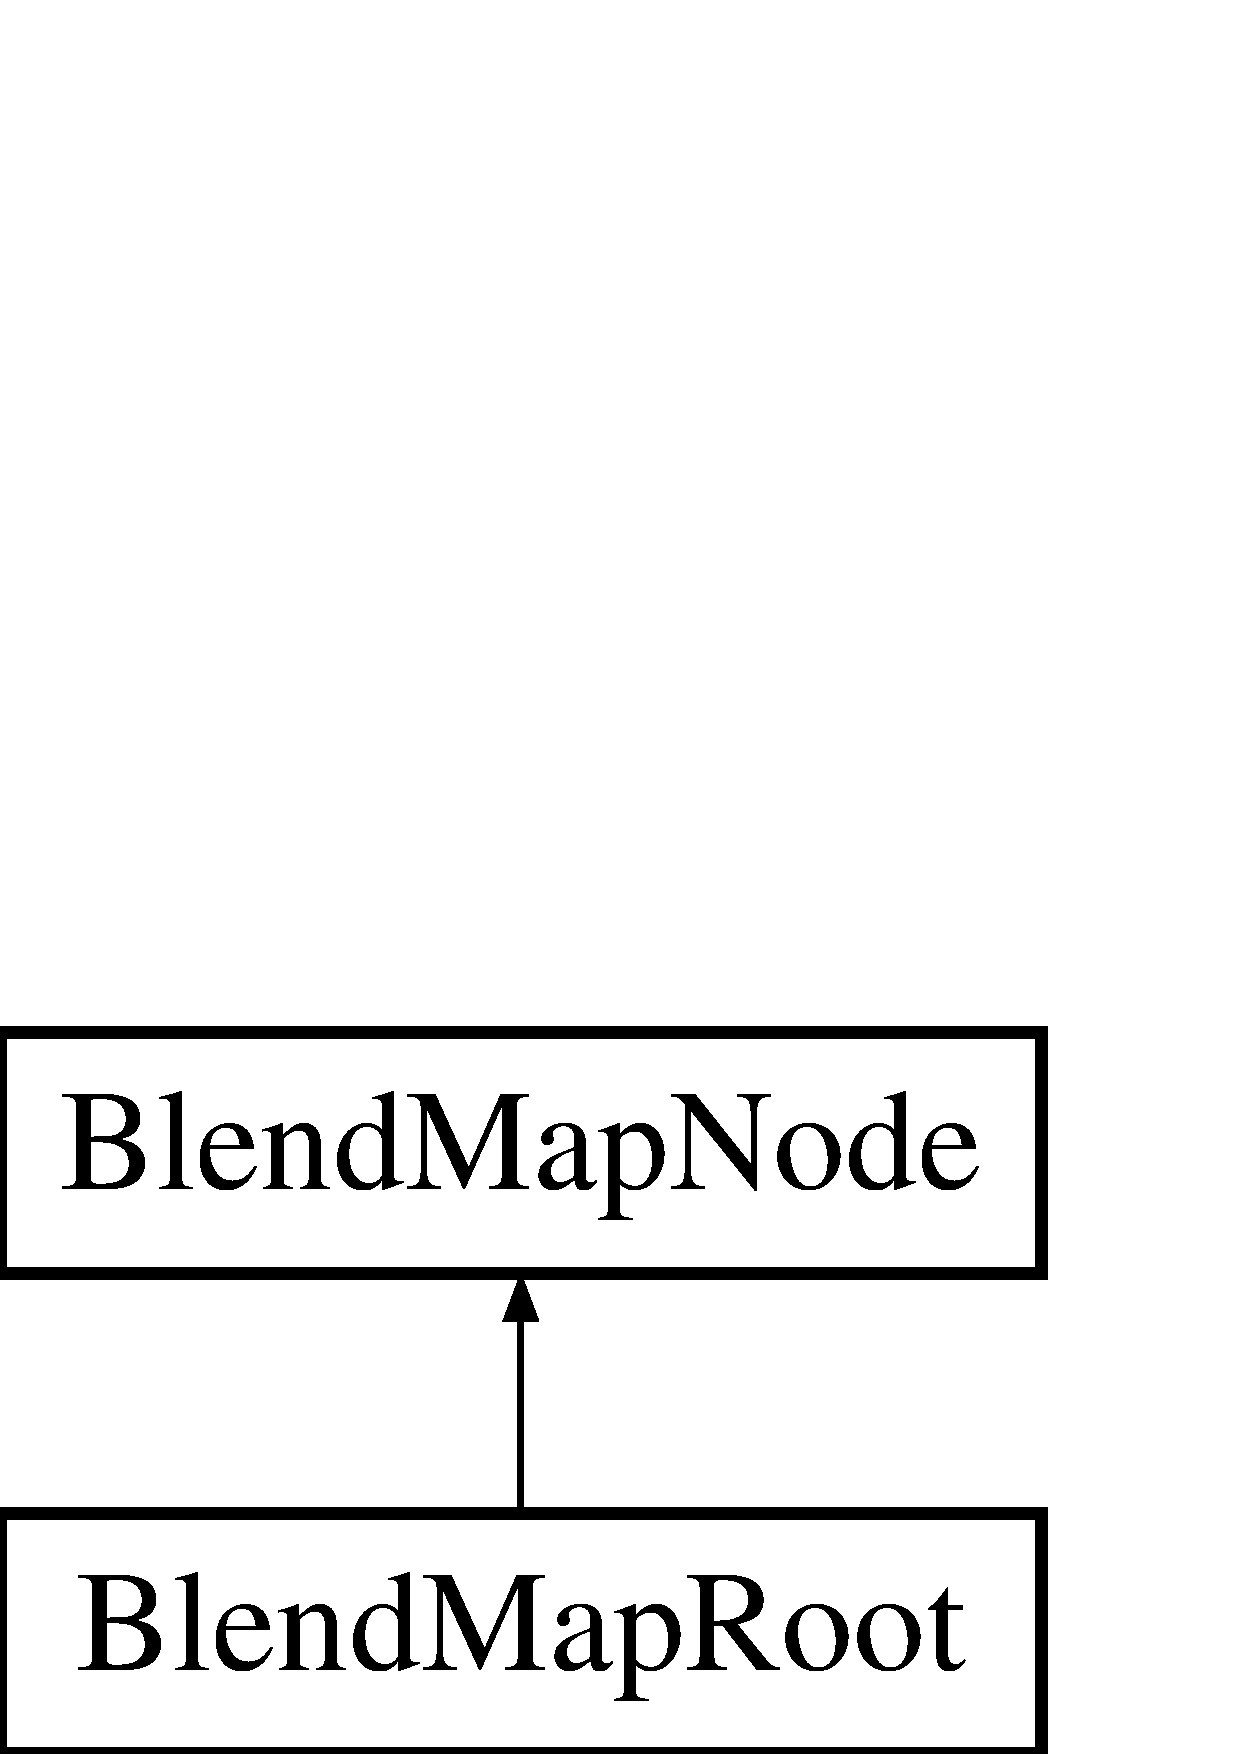
\includegraphics[height=2.000000cm]{struct_blend_map_node}
\end{center}
\end{figure}
\subsection*{Public Member Functions}
\begin{DoxyCompactItemize}
\item 
\mbox{\Hypertarget{struct_blend_map_node_a81d8023d5abe4d61e596511ff9338e1f}\label{struct_blend_map_node_a81d8023d5abe4d61e596511ff9338e1f}} 
void {\bfseries cleanup} (int type)
\item 
\mbox{\Hypertarget{struct_blend_map_node_ac89dbc56181a3eb63f57aac3a5784fe7}\label{struct_blend_map_node_ac89dbc56181a3eb63f57aac3a5784fe7}} 
void {\bfseries splitsolid} (uchar \&type, uchar val)
\end{DoxyCompactItemize}
\subsection*{Public Attributes}
\begin{DoxyCompactItemize}
\item 
\mbox{\Hypertarget{struct_blend_map_node_aafabf99c170ee0343131fa06919ae770}\label{struct_blend_map_node_aafabf99c170ee0343131fa06919ae770}} 
\begin{tabbing}
xx\=xx\=xx\=xx\=xx\=xx\=xx\=xx\=xx\=\kill
union \{\\
\>\hyperlink{struct_blend_map_branch}{BlendMapBranch} $\ast$ {\bfseries branch}\\
\>\hyperlink{struct_blend_map_solid}{BlendMapSolid} $\ast$ {\bfseries solid}\\
\>\hyperlink{struct_blend_map_image}{BlendMapImage} $\ast$ {\bfseries image}\\
\}; \\

\end{tabbing}\end{DoxyCompactItemize}


The documentation for this struct was generated from the following file\+:\begin{DoxyCompactItemize}
\item 
H\+:/\+Rival\+Engine/\+Rival\+\_\+\+Game\+\_\+\+Engine\+\_\+\+G\+I\+T/\+Rival3dengine/source/engine/blend.\+cpp\end{DoxyCompactItemize}

\hypertarget{struct_blend_map_root}{}\section{Blend\+Map\+Root Struct Reference}
\label{struct_blend_map_root}\index{Blend\+Map\+Root@{Blend\+Map\+Root}}
Inheritance diagram for Blend\+Map\+Root\+:\begin{figure}[H]
\begin{center}
\leavevmode
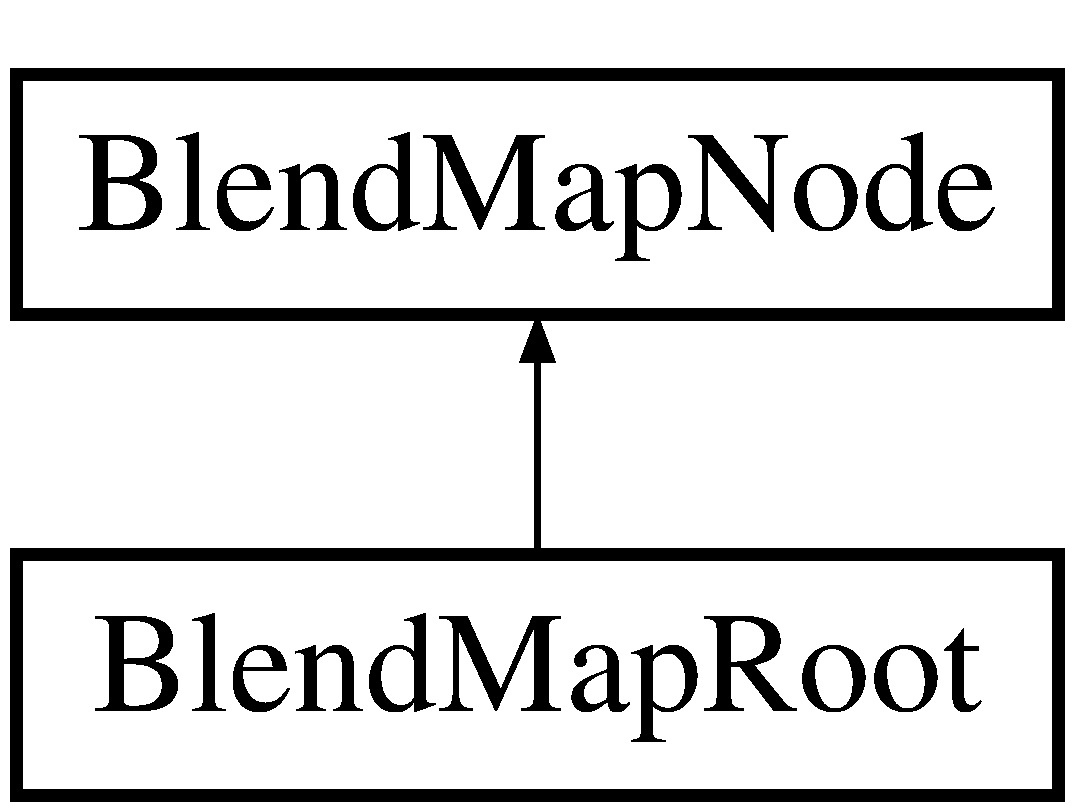
\includegraphics[height=2.000000cm]{struct_blend_map_root}
\end{center}
\end{figure}
\subsection*{Public Member Functions}
\begin{DoxyCompactItemize}
\item 
\mbox{\Hypertarget{struct_blend_map_root_a34d41ce7a40167aa0a843117409360c5}\label{struct_blend_map_root_a34d41ce7a40167aa0a843117409360c5}} 
{\bfseries Blend\+Map\+Root} (uchar type, const \hyperlink{struct_blend_map_node}{Blend\+Map\+Node} \&\hyperlink{structnode}{node})
\item 
\mbox{\Hypertarget{struct_blend_map_root_a69fa8e8de5442dd66b46bf8617c32e75}\label{struct_blend_map_root_a69fa8e8de5442dd66b46bf8617c32e75}} 
void {\bfseries cleanup} ()
\item 
\mbox{\Hypertarget{struct_blend_map_root_a9be01279e5d8befb9016f43e6dfa76f8}\label{struct_blend_map_root_a9be01279e5d8befb9016f43e6dfa76f8}} 
void {\bfseries shrink} (int quadrant)
\end{DoxyCompactItemize}
\subsection*{Public Attributes}
\begin{DoxyCompactItemize}
\item 
\mbox{\Hypertarget{struct_blend_map_root_acaeed8fc93bd2f2f88e95572b3d6386a}\label{struct_blend_map_root_acaeed8fc93bd2f2f88e95572b3d6386a}} 
uchar {\bfseries type}
\end{DoxyCompactItemize}


The documentation for this struct was generated from the following file\+:\begin{DoxyCompactItemize}
\item 
H\+:/\+Rival\+Engine/\+Rival\+\_\+\+Game\+\_\+\+Engine\+\_\+\+G\+I\+T/\+Rival3dengine/source/engine/blend.\+cpp\end{DoxyCompactItemize}

\hypertarget{struct_blend_map_solid}{}\section{Blend\+Map\+Solid Struct Reference}
\label{struct_blend_map_solid}\index{Blend\+Map\+Solid@{Blend\+Map\+Solid}}
\subsection*{Public Member Functions}
\begin{DoxyCompactItemize}
\item 
\mbox{\Hypertarget{struct_blend_map_solid_a98bce9b25af361c3d726078bfa8625fd}\label{struct_blend_map_solid_a98bce9b25af361c3d726078bfa8625fd}} 
{\bfseries Blend\+Map\+Solid} (uchar val)
\end{DoxyCompactItemize}
\subsection*{Public Attributes}
\begin{DoxyCompactItemize}
\item 
\mbox{\Hypertarget{struct_blend_map_solid_a45364c3517a30d9068f8ce8368b63879}\label{struct_blend_map_solid_a45364c3517a30d9068f8ce8368b63879}} 
uchar {\bfseries val}
\end{DoxyCompactItemize}


The documentation for this struct was generated from the following file\+:\begin{DoxyCompactItemize}
\item 
H\+:/\+Rival\+Engine/\+Rival\+\_\+\+Game\+\_\+\+Engine\+\_\+\+G\+I\+T/\+Rival3dengine/source/engine/blend.\+cpp\end{DoxyCompactItemize}

\hypertarget{struct_blend_texture}{}\section{Blend\+Texture Struct Reference}
\label{struct_blend_texture}\index{Blend\+Texture@{Blend\+Texture}}
\subsection*{Public Member Functions}
\begin{DoxyCompactItemize}
\item 
\mbox{\Hypertarget{struct_blend_texture_ae09f60147b3b3257fd3f49cfb871aadd}\label{struct_blend_texture_ae09f60147b3b3257fd3f49cfb871aadd}} 
bool {\bfseries setup} (int sz)
\item 
\mbox{\Hypertarget{struct_blend_texture_a090cea35ba21a821f1c2975bac15c666}\label{struct_blend_texture_a090cea35ba21a821f1c2975bac15c666}} 
void {\bfseries cleanup} ()
\item 
\mbox{\Hypertarget{struct_blend_texture_a86469062b9789d14377eee326dcfb0d8}\label{struct_blend_texture_a86469062b9789d14377eee326dcfb0d8}} 
bool {\bfseries contains} (int px, int py) const
\item 
\mbox{\Hypertarget{struct_blend_texture_a2ef925c7d30a00682487ba0d475bda60}\label{struct_blend_texture_a2ef925c7d30a00682487ba0d475bda60}} 
bool {\bfseries contains} (const \hyperlink{structivec}{ivec} \&p) const
\end{DoxyCompactItemize}
\subsection*{Public Attributes}
\begin{DoxyCompactItemize}
\item 
\mbox{\Hypertarget{struct_blend_texture_ae1d433263240ffc9dba95c2e56821eb8}\label{struct_blend_texture_ae1d433263240ffc9dba95c2e56821eb8}} 
int {\bfseries x}
\item 
\mbox{\Hypertarget{struct_blend_texture_a206f9a7277a7f9646b5efd446a4a0f9d}\label{struct_blend_texture_a206f9a7277a7f9646b5efd446a4a0f9d}} 
int {\bfseries y}
\item 
\mbox{\Hypertarget{struct_blend_texture_a6042338de4bb337adf4117bc645d2960}\label{struct_blend_texture_a6042338de4bb337adf4117bc645d2960}} 
int {\bfseries size}
\item 
\mbox{\Hypertarget{struct_blend_texture_af4d1b994390426b9214d04c22eb1df4f}\label{struct_blend_texture_af4d1b994390426b9214d04c22eb1df4f}} 
uchar $\ast$ {\bfseries data}
\item 
\mbox{\Hypertarget{struct_blend_texture_acccbe6e2ffc2073fc354f9d4e61e7ee9}\label{struct_blend_texture_acccbe6e2ffc2073fc354f9d4e61e7ee9}} 
G\+Luint {\bfseries tex}
\item 
\mbox{\Hypertarget{struct_blend_texture_a149774587c5eb2fb694ebf18c91f7ec5}\label{struct_blend_texture_a149774587c5eb2fb694ebf18c91f7ec5}} 
G\+Lenum {\bfseries format}
\item 
\mbox{\Hypertarget{struct_blend_texture_aaae475ca2a21620d237e9318e17b5f65}\label{struct_blend_texture_aaae475ca2a21620d237e9318e17b5f65}} 
bool {\bfseries valid}
\end{DoxyCompactItemize}


The documentation for this struct was generated from the following file\+:\begin{DoxyCompactItemize}
\item 
H\+:/\+Rival\+Engine/\+Rival\+\_\+\+Game\+\_\+\+Engine\+\_\+\+G\+I\+T/\+Rival3dengine/source/engine/blend.\+cpp\end{DoxyCompactItemize}

\hypertarget{structblock3}{}\section{block3 Struct Reference}
\label{structblock3}\index{block3@{block3}}
\subsection*{Public Member Functions}
\begin{DoxyCompactItemize}
\item 
\mbox{\Hypertarget{structblock3_a6a8f0d4d661fee239ff5be5c63c30fc3}\label{structblock3_a6a8f0d4d661fee239ff5be5c63c30fc3}} 
{\bfseries block3} (const \hyperlink{structselinfo}{selinfo} \&sel)
\item 
\mbox{\Hypertarget{structblock3_adf0824981bc64c9e38d0992216907b3f}\label{structblock3_adf0824981bc64c9e38d0992216907b3f}} 
\hyperlink{structcube}{cube} $\ast$ {\bfseries c} ()
\item 
\mbox{\Hypertarget{structblock3_ab61c08cdf7ad396f4241f299c8e1b45b}\label{structblock3_ab61c08cdf7ad396f4241f299c8e1b45b}} 
int {\bfseries size} () const
\end{DoxyCompactItemize}
\subsection*{Public Attributes}
\begin{DoxyCompactItemize}
\item 
\mbox{\Hypertarget{structblock3_a0791a74c1bed41349ab86e7b2dea2788}\label{structblock3_a0791a74c1bed41349ab86e7b2dea2788}} 
\hyperlink{structivec}{ivec} {\bfseries o}
\item 
\mbox{\Hypertarget{structblock3_a6c3aa35448d7552c040881c1bd0e4aa6}\label{structblock3_a6c3aa35448d7552c040881c1bd0e4aa6}} 
\hyperlink{structivec}{ivec} {\bfseries s}
\item 
\mbox{\Hypertarget{structblock3_ad8e892ec4498e1738d6a5c074b3b0d0b}\label{structblock3_ad8e892ec4498e1738d6a5c074b3b0d0b}} 
int {\bfseries grid}
\item 
\mbox{\Hypertarget{structblock3_a702dec30718798d2ec8c9070d37dcb44}\label{structblock3_a702dec30718798d2ec8c9070d37dcb44}} 
int {\bfseries orient}
\end{DoxyCompactItemize}


The documentation for this struct was generated from the following file\+:\begin{DoxyCompactItemize}
\item 
H\+:/\+Rival\+Engine/\+Rival\+\_\+\+Game\+\_\+\+Engine\+\_\+\+G\+I\+T/\+Rival3dengine/source/engine/octa.\+h\end{DoxyCompactItemize}

\hypertarget{structskelmodel_1_1boneinfo}{}\section{skelmodel\+:\+:boneinfo Struct Reference}
\label{structskelmodel_1_1boneinfo}\index{skelmodel\+::boneinfo@{skelmodel\+::boneinfo}}
\subsection*{Public Attributes}
\begin{DoxyCompactItemize}
\item 
\mbox{\Hypertarget{structskelmodel_1_1boneinfo_a7c79f04ae176def99a9ef8e8c145d63b}\label{structskelmodel_1_1boneinfo_a7c79f04ae176def99a9ef8e8c145d63b}} 
const char $\ast$ {\bfseries name}
\item 
\mbox{\Hypertarget{structskelmodel_1_1boneinfo_ac2d292bfc7c6d1bb52b782e79b5a6faa}\label{structskelmodel_1_1boneinfo_ac2d292bfc7c6d1bb52b782e79b5a6faa}} 
int {\bfseries parent}
\item 
\mbox{\Hypertarget{structskelmodel_1_1boneinfo_a273d1f713a813df4d6b93b0f3ec16a30}\label{structskelmodel_1_1boneinfo_a273d1f713a813df4d6b93b0f3ec16a30}} 
int {\bfseries children}
\item 
\mbox{\Hypertarget{structskelmodel_1_1boneinfo_ad0bfa69ecb73d26d08a3b156ad4c2ffd}\label{structskelmodel_1_1boneinfo_ad0bfa69ecb73d26d08a3b156ad4c2ffd}} 
int {\bfseries next}
\item 
\mbox{\Hypertarget{structskelmodel_1_1boneinfo_ad414ec14e5cf49f570ec83f920ef1987}\label{structskelmodel_1_1boneinfo_ad414ec14e5cf49f570ec83f920ef1987}} 
int {\bfseries group}
\item 
\mbox{\Hypertarget{structskelmodel_1_1boneinfo_ac4a1ceb727189c5faaec738379af6075}\label{structskelmodel_1_1boneinfo_ac4a1ceb727189c5faaec738379af6075}} 
int {\bfseries scheduled}
\item 
\mbox{\Hypertarget{structskelmodel_1_1boneinfo_ad5b8e5d5e8a1f46c2cf41aa7fe26210d}\label{structskelmodel_1_1boneinfo_ad5b8e5d5e8a1f46c2cf41aa7fe26210d}} 
int {\bfseries interpindex}
\item 
\mbox{\Hypertarget{structskelmodel_1_1boneinfo_a5c42d00972cde4174f35d5bf9335a8ff}\label{structskelmodel_1_1boneinfo_a5c42d00972cde4174f35d5bf9335a8ff}} 
int {\bfseries interpparent}
\item 
\mbox{\Hypertarget{structskelmodel_1_1boneinfo_a7d6f075388ab9b73a2fc37ec90875703}\label{structskelmodel_1_1boneinfo_a7d6f075388ab9b73a2fc37ec90875703}} 
int {\bfseries ragdollindex}
\item 
\mbox{\Hypertarget{structskelmodel_1_1boneinfo_a4ffc5130c8f712e89c0756a4fa70b3ba}\label{structskelmodel_1_1boneinfo_a4ffc5130c8f712e89c0756a4fa70b3ba}} 
int {\bfseries correctindex}
\item 
\mbox{\Hypertarget{structskelmodel_1_1boneinfo_a5fc8ea4cbcd7dee23ef4d6f301013248}\label{structskelmodel_1_1boneinfo_a5fc8ea4cbcd7dee23ef4d6f301013248}} 
float {\bfseries pitchscale}
\item 
\mbox{\Hypertarget{structskelmodel_1_1boneinfo_a4d33ef11f15c6030d760cfbaa183ee7a}\label{structskelmodel_1_1boneinfo_a4d33ef11f15c6030d760cfbaa183ee7a}} 
float {\bfseries pitchoffset}
\item 
\mbox{\Hypertarget{structskelmodel_1_1boneinfo_abce2d8858e3c1eb479d0d891da5e0ff8}\label{structskelmodel_1_1boneinfo_abce2d8858e3c1eb479d0d891da5e0ff8}} 
float {\bfseries pitchmin}
\item 
\mbox{\Hypertarget{structskelmodel_1_1boneinfo_a46422d32c2a95ee3f0eb30202ba3bdcd}\label{structskelmodel_1_1boneinfo_a46422d32c2a95ee3f0eb30202ba3bdcd}} 
float {\bfseries pitchmax}
\item 
\mbox{\Hypertarget{structskelmodel_1_1boneinfo_a7515ba7fe742ddad1f3d10f9b879f9c0}\label{structskelmodel_1_1boneinfo_a7515ba7fe742ddad1f3d10f9b879f9c0}} 
\hyperlink{structdualquat}{dualquat} {\bfseries base}
\item 
\mbox{\Hypertarget{structskelmodel_1_1boneinfo_a0ab86759a52bd130b02feb11d7451a5a}\label{structskelmodel_1_1boneinfo_a0ab86759a52bd130b02feb11d7451a5a}} 
\hyperlink{structdualquat}{dualquat} {\bfseries invbase}
\end{DoxyCompactItemize}


The documentation for this struct was generated from the following file\+:\begin{DoxyCompactItemize}
\item 
H\+:/\+Rival\+Engine/\+Rival\+\_\+\+Game\+\_\+\+Engine\+\_\+\+G\+I\+T/\+Rival3dengine/source/engine/skelmodel.\+h\end{DoxyCompactItemize}

\hypertarget{struct_u_i_1_1_bordered_image}{}\section{UI\+:\+:Bordered\+Image Struct Reference}
\label{struct_u_i_1_1_bordered_image}\index{U\+I\+::\+Bordered\+Image@{U\+I\+::\+Bordered\+Image}}
Inheritance diagram for UI\+:\+:Bordered\+Image\+:\begin{figure}[H]
\begin{center}
\leavevmode
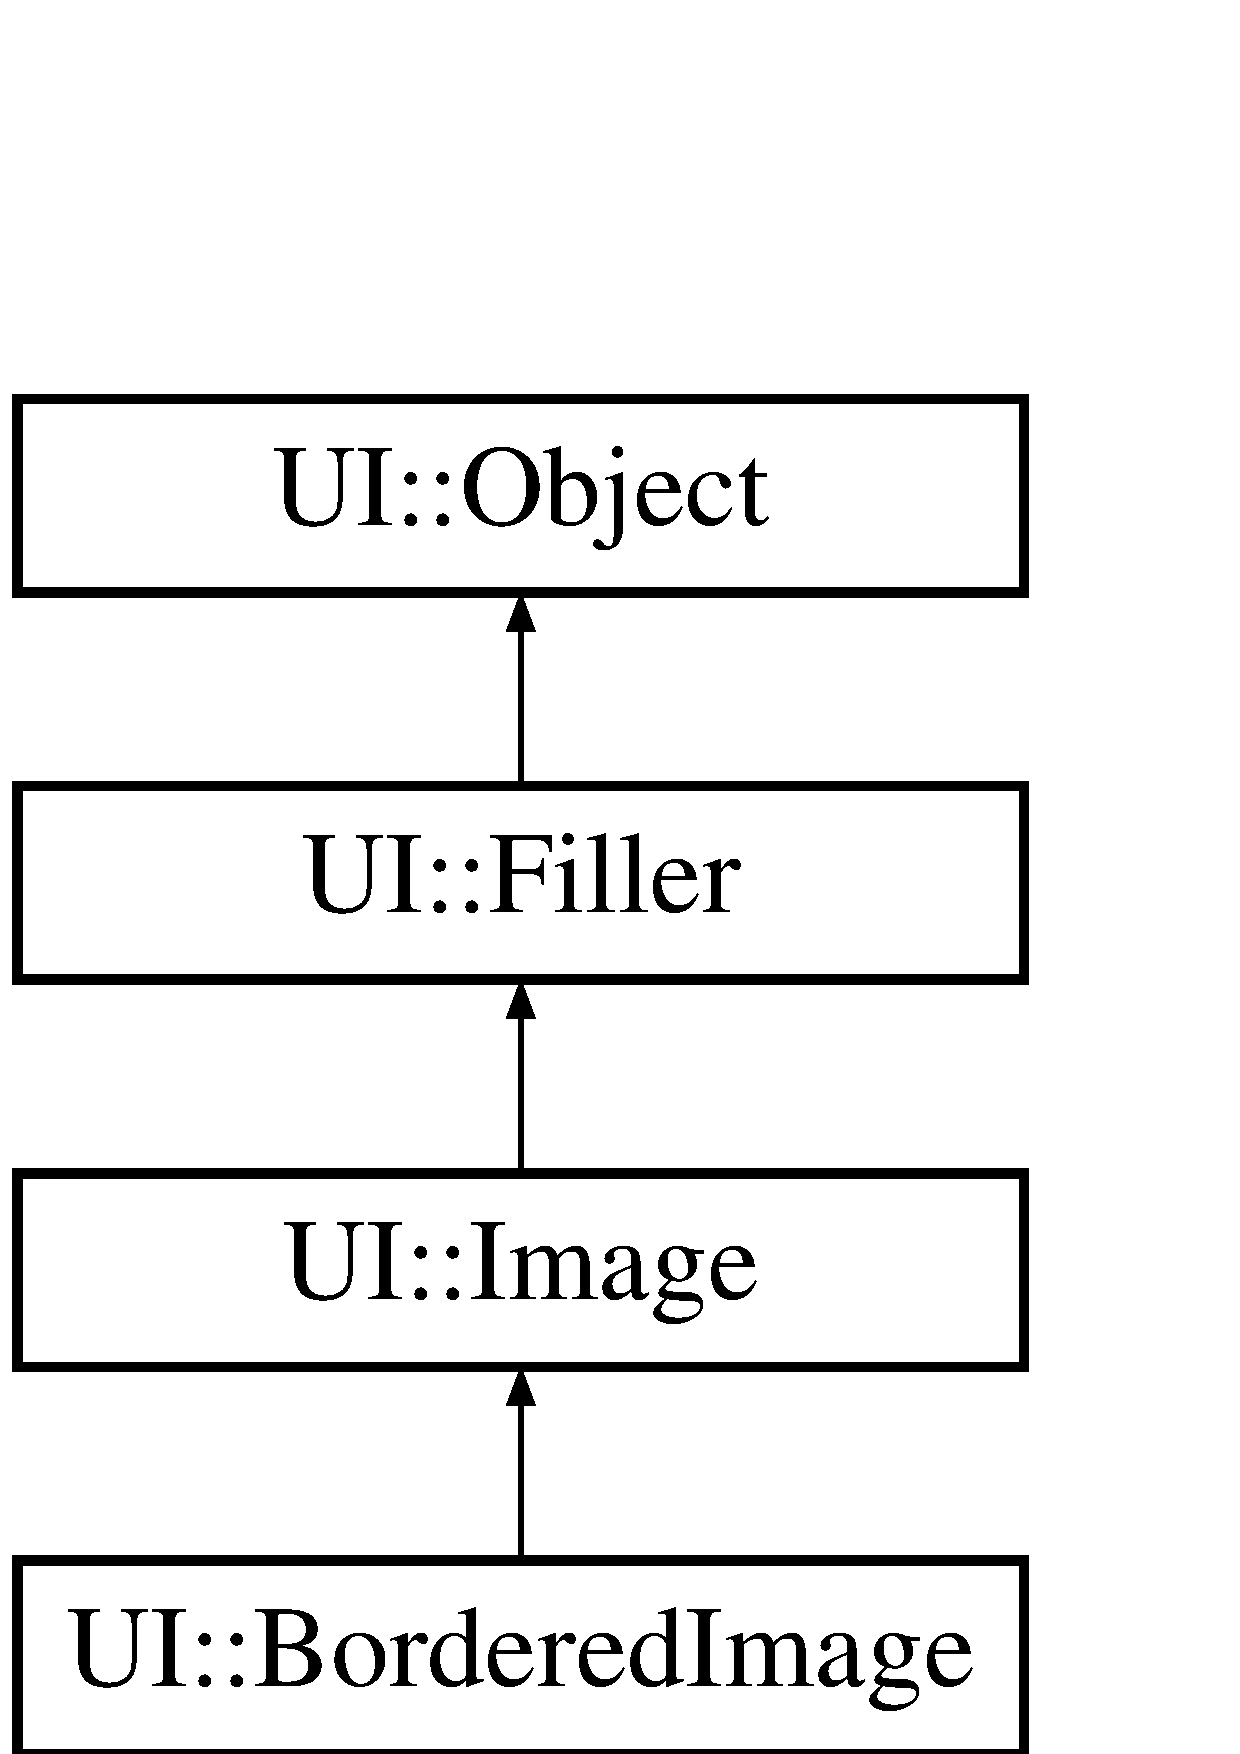
\includegraphics[height=4.000000cm]{struct_u_i_1_1_bordered_image}
\end{center}
\end{figure}
\subsection*{Public Member Functions}
\begin{DoxyCompactItemize}
\item 
\mbox{\Hypertarget{struct_u_i_1_1_bordered_image_a11361a1d4292d5c02358ca1defd5e89f}\label{struct_u_i_1_1_bordered_image_a11361a1d4292d5c02358ca1defd5e89f}} 
void {\bfseries setup} (\hyperlink{struct_texture}{Texture} $\ast$tex\+\_\+, float texborder\+\_\+, float screenborder\+\_\+)
\item 
\mbox{\Hypertarget{struct_u_i_1_1_bordered_image_a1c4c42ec131df0b6d7a53ace42d84f5a}\label{struct_u_i_1_1_bordered_image_a1c4c42ec131df0b6d7a53ace42d84f5a}} 
const char $\ast$ {\bfseries gettype} () const
\item 
\mbox{\Hypertarget{struct_u_i_1_1_bordered_image_ae0c062b65f37363cc2fa092324705cbf}\label{struct_u_i_1_1_bordered_image_ae0c062b65f37363cc2fa092324705cbf}} 
bool {\bfseries target} (float cx, float cy)
\item 
\mbox{\Hypertarget{struct_u_i_1_1_bordered_image_a4f1aae7577b5a4428633589c1bf1f08f}\label{struct_u_i_1_1_bordered_image_a4f1aae7577b5a4428633589c1bf1f08f}} 
void {\bfseries draw} (float sx, float sy)
\end{DoxyCompactItemize}
\subsection*{Static Public Member Functions}
\begin{DoxyCompactItemize}
\item 
\mbox{\Hypertarget{struct_u_i_1_1_bordered_image_afa941a22d447e9812109b0a3091eb9c4}\label{struct_u_i_1_1_bordered_image_afa941a22d447e9812109b0a3091eb9c4}} 
static const char $\ast$ {\bfseries typestr} ()
\end{DoxyCompactItemize}
\subsection*{Public Attributes}
\begin{DoxyCompactItemize}
\item 
\mbox{\Hypertarget{struct_u_i_1_1_bordered_image_a82119c3e47440b8df03bd85933767dcf}\label{struct_u_i_1_1_bordered_image_a82119c3e47440b8df03bd85933767dcf}} 
float {\bfseries texborder}
\item 
\mbox{\Hypertarget{struct_u_i_1_1_bordered_image_aa0da7ec74ecffa449c8b6e1628b759eb}\label{struct_u_i_1_1_bordered_image_aa0da7ec74ecffa449c8b6e1628b759eb}} 
float {\bfseries screenborder}
\end{DoxyCompactItemize}
\subsection*{Additional Inherited Members}


The documentation for this struct was generated from the following file\+:\begin{DoxyCompactItemize}
\item 
H\+:/\+Rival\+Engine/\+Rival\+\_\+\+Game\+\_\+\+Engine\+\_\+\+G\+I\+T/\+Rival3dengine/source/engine/ui.\+cpp\end{DoxyCompactItemize}

\hypertarget{structgame_1_1bouncer}{}\section{game\+:\+:bouncer Struct Reference}
\label{structgame_1_1bouncer}\index{game\+::bouncer@{game\+::bouncer}}
Inheritance diagram for game\+:\+:bouncer\+:\begin{figure}[H]
\begin{center}
\leavevmode
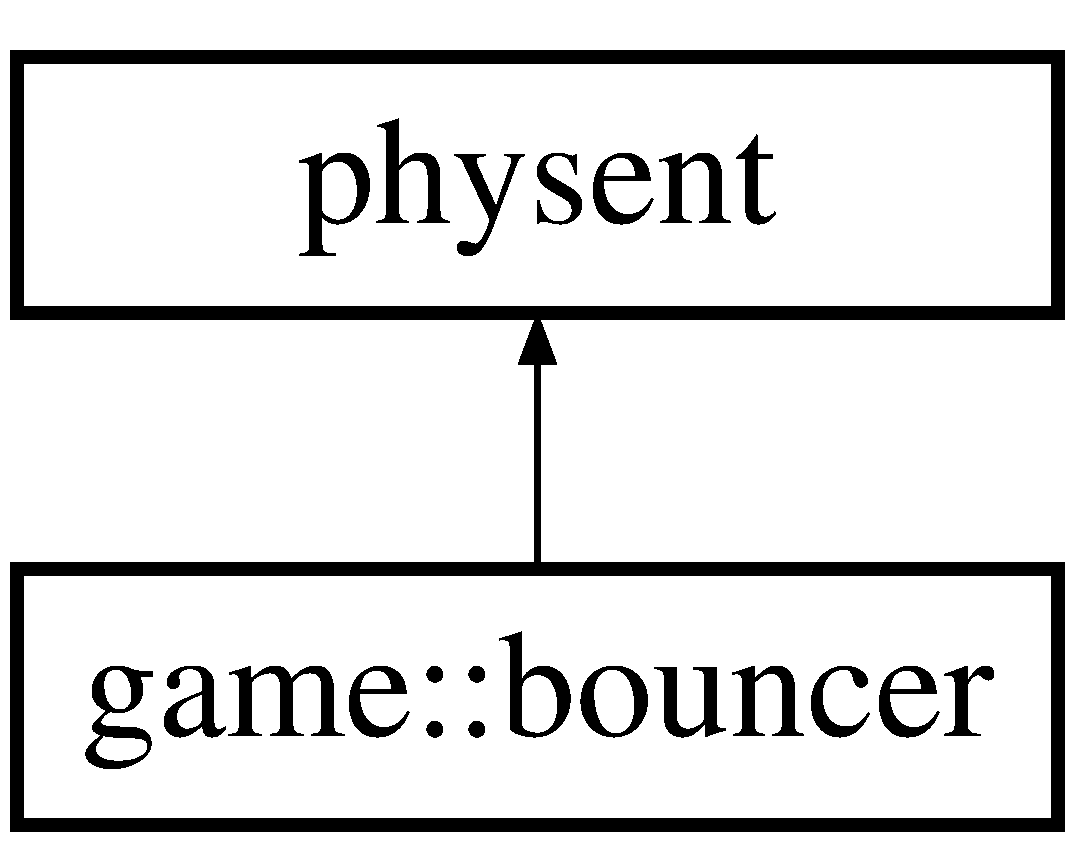
\includegraphics[height=2.000000cm]{structgame_1_1bouncer}
\end{center}
\end{figure}
\subsection*{Public Attributes}
\begin{DoxyCompactItemize}
\item 
\mbox{\Hypertarget{structgame_1_1bouncer_a2cc7b6b0e1a877ca0b5fc7917365b5e5}\label{structgame_1_1bouncer_a2cc7b6b0e1a877ca0b5fc7917365b5e5}} 
int {\bfseries lifetime}
\item 
\mbox{\Hypertarget{structgame_1_1bouncer_acc4edbfc630e3b759833a681d15e4158}\label{structgame_1_1bouncer_acc4edbfc630e3b759833a681d15e4158}} 
int {\bfseries bounces}
\item 
\mbox{\Hypertarget{structgame_1_1bouncer_a96426e908a0652f26138a7473084cf40}\label{structgame_1_1bouncer_a96426e908a0652f26138a7473084cf40}} 
float {\bfseries lastyaw}
\item 
\mbox{\Hypertarget{structgame_1_1bouncer_a685cf2280b33854ff1fa0a889386aac0}\label{structgame_1_1bouncer_a685cf2280b33854ff1fa0a889386aac0}} 
float {\bfseries roll}
\item 
\mbox{\Hypertarget{structgame_1_1bouncer_abc485f2956f52f71489ddd68adf80958}\label{structgame_1_1bouncer_abc485f2956f52f71489ddd68adf80958}} 
bool {\bfseries local}
\item 
\mbox{\Hypertarget{structgame_1_1bouncer_a4b5ed8a47df43ea3f017ed2a85556a83}\label{structgame_1_1bouncer_a4b5ed8a47df43ea3f017ed2a85556a83}} 
\hyperlink{structgameent}{gameent} $\ast$ {\bfseries owner}
\item 
\mbox{\Hypertarget{structgame_1_1bouncer_a78ca5444a43487d89ed30cbbbc15b959}\label{structgame_1_1bouncer_a78ca5444a43487d89ed30cbbbc15b959}} 
int {\bfseries bouncetype}
\item 
\mbox{\Hypertarget{structgame_1_1bouncer_a852f0a903ee4275a06dfc32dddb6c63d}\label{structgame_1_1bouncer_a852f0a903ee4275a06dfc32dddb6c63d}} 
int {\bfseries variant}
\item 
\mbox{\Hypertarget{structgame_1_1bouncer_a94679393bacdf83bf64b7f8082854e74}\label{structgame_1_1bouncer_a94679393bacdf83bf64b7f8082854e74}} 
\hyperlink{structvec}{vec} {\bfseries offset}
\item 
\mbox{\Hypertarget{structgame_1_1bouncer_a4636f6072f94538d29ef1d16d4f60765}\label{structgame_1_1bouncer_a4636f6072f94538d29ef1d16d4f60765}} 
int {\bfseries offsetmillis}
\item 
\mbox{\Hypertarget{structgame_1_1bouncer_a6960ae69f49b7a491b891668ce8d57fc}\label{structgame_1_1bouncer_a6960ae69f49b7a491b891668ce8d57fc}} 
int {\bfseries id}
\end{DoxyCompactItemize}
\subsection*{Additional Inherited Members}


The documentation for this struct was generated from the following file\+:\begin{DoxyCompactItemize}
\item 
H\+:/\+Rival\+Engine/\+Rival\+\_\+\+Game\+\_\+\+Engine\+\_\+\+G\+I\+T/\+Rival3dengine/source/game/weapon.\+cpp\end{DoxyCompactItemize}

\hypertarget{structbt_t_e_m_p_m_e_l_o_o_k_a_t_l_a_t_e_r}{}\section{bt\+T\+E\+M\+P\+M\+E\+L\+O\+O\+K\+A\+T\+L\+A\+T\+ER Struct Reference}
\label{structbt_t_e_m_p_m_e_l_o_o_k_a_t_l_a_t_e_r}\index{bt\+T\+E\+M\+P\+M\+E\+L\+O\+O\+K\+A\+T\+L\+A\+T\+ER@{bt\+T\+E\+M\+P\+M\+E\+L\+O\+O\+K\+A\+T\+L\+A\+T\+ER}}
\subsection*{Public Attributes}
\begin{DoxyCompactItemize}
\item 
\mbox{\Hypertarget{structbt_t_e_m_p_m_e_l_o_o_k_a_t_l_a_t_e_r_a31a2f7aa471ca04175f6d0957c5d9995}\label{structbt_t_e_m_p_m_e_l_o_o_k_a_t_l_a_t_e_r_a31a2f7aa471ca04175f6d0957c5d9995}} 
\hyperlink{structvector}{vector}$<$ bt\+Rigid\+Body $\ast$ $>$ {\bfseries bodies}
\item 
\mbox{\Hypertarget{structbt_t_e_m_p_m_e_l_o_o_k_a_t_l_a_t_e_r_abb9f2dbef2607b7693f09a9900a391ca}\label{structbt_t_e_m_p_m_e_l_o_o_k_a_t_l_a_t_e_r_abb9f2dbef2607b7693f09a9900a391ca}} 
\hyperlink{structvector}{vector}$<$ bt\+Typed\+Constraint $\ast$ $>$ {\bfseries contraints}
\end{DoxyCompactItemize}


The documentation for this struct was generated from the following file\+:\begin{DoxyCompactItemize}
\item 
H\+:/\+Rival\+Engine/\+Rival\+\_\+\+Game\+\_\+\+Engine\+\_\+\+G\+I\+T/\+Rival3dengine/source/engine/A\+J\+M\+Phys.\+h\end{DoxyCompactItemize}

\hypertarget{structgame_1_1bulletmovable}{}\section{game\+:\+:bulletmovable Struct Reference}
\label{structgame_1_1bulletmovable}\index{game\+::bulletmovable@{game\+::bulletmovable}}
\subsection*{Public Member Functions}
\begin{DoxyCompactItemize}
\item 
\mbox{\Hypertarget{structgame_1_1bulletmovable_a9cb266b6e5ade1870638c54a21da1c70}\label{structgame_1_1bulletmovable_a9cb266b6e5ade1870638c54a21da1c70}} 
{\bfseries bulletmovable} (const \hyperlink{structentity}{entity} \&e)
\end{DoxyCompactItemize}
\subsection*{Public Attributes}
\begin{DoxyCompactItemize}
\item 
\mbox{\Hypertarget{structgame_1_1bulletmovable_ad248b5cebbcc72da902ace252d1569d3}\label{structgame_1_1bulletmovable_ad248b5cebbcc72da902ace252d1569d3}} 
int {\bfseries etype}
\item 
\mbox{\Hypertarget{structgame_1_1bulletmovable_a3ce7b403eb503a74a5715a68c587b98a}\label{structgame_1_1bulletmovable_a3ce7b403eb503a74a5715a68c587b98a}} 
int {\bfseries mapmodel}
\item 
\mbox{\Hypertarget{structgame_1_1bulletmovable_a9f30fa9649c5b1b060f7df5df71d3335}\label{structgame_1_1bulletmovable_a9f30fa9649c5b1b060f7df5df71d3335}} 
int {\bfseries weight}
\item 
\mbox{\Hypertarget{structgame_1_1bulletmovable_adaa62f77b522d18346f4fa1f4b8df44c}\label{structgame_1_1bulletmovable_adaa62f77b522d18346f4fa1f4b8df44c}} 
float {\bfseries yaw}
\item 
\mbox{\Hypertarget{structgame_1_1bulletmovable_a779b9138c82b225d79cb6a902bf2056f}\label{structgame_1_1bulletmovable_a779b9138c82b225d79cb6a902bf2056f}} 
float {\bfseries pitch}
\item 
\mbox{\Hypertarget{structgame_1_1bulletmovable_a8388285c4c000e711cf40df9e3d32e50}\label{structgame_1_1bulletmovable_a8388285c4c000e711cf40df9e3d32e50}} 
float {\bfseries roll}
\item 
\mbox{\Hypertarget{structgame_1_1bulletmovable_a0ddec26746c32b51aebad568f5c976df}\label{structgame_1_1bulletmovable_a0ddec26746c32b51aebad568f5c976df}} 
\hyperlink{structvec}{vec} {\bfseries o}
\item 
\mbox{\Hypertarget{structgame_1_1bulletmovable_a86329554af2d1db43c87af441d9eded1}\label{structgame_1_1bulletmovable_a86329554af2d1db43c87af441d9eded1}} 
\hyperlink{structvec}{vec} {\bfseries radius}
\item 
\mbox{\Hypertarget{structgame_1_1bulletmovable_ac4cee1b1aa4a467bbfd5011ccd62de1d}\label{structgame_1_1bulletmovable_ac4cee1b1aa4a467bbfd5011ccd62de1d}} 
bt\+Rigid\+Body $\ast$ {\bfseries body}
\end{DoxyCompactItemize}


The documentation for this struct was generated from the following file\+:\begin{DoxyCompactItemize}
\item 
H\+:/\+Rival\+Engine/\+Rival\+\_\+\+Game\+\_\+\+Engine\+\_\+\+G\+I\+T/\+Rival3dengine/source/game/A\+J\+Mmovable.\+cpp\end{DoxyCompactItemize}

\hypertarget{structbulletobj}{}\section{bulletobj Struct Reference}
\label{structbulletobj}\index{bulletobj@{bulletobj}}
\subsection*{Public Member Functions}
\begin{DoxyCompactItemize}
\item 
\mbox{\Hypertarget{structbulletobj_a3e1d541bff689c0390f9148378095136}\label{structbulletobj_a3e1d541bff689c0390f9148378095136}} 
void {\bfseries move} (\hyperlink{structvec}{vec} im)
\item 
\mbox{\Hypertarget{structbulletobj_aa5ee748fb56578ba86fcf5a6fae6e66c}\label{structbulletobj_aa5ee748fb56578ba86fcf5a6fae6e66c}} 
void {\bfseries rotate} (\hyperlink{structvec}{vec} im)
\item 
\mbox{\Hypertarget{structbulletobj_aba11c4ec444f432b44f382702217e6c2}\label{structbulletobj_aba11c4ec444f432b44f382702217e6c2}} 
void {\bfseries moveto} (\hyperlink{structvec}{vec} \+\_\+o)
\end{DoxyCompactItemize}
\subsection*{Public Attributes}
\begin{DoxyCompactItemize}
\item 
\mbox{\Hypertarget{structbulletobj_a795fb9d432053b7f1b7cf017e7927d15}\label{structbulletobj_a795fb9d432053b7f1b7cf017e7927d15}} 
bt\+Rigid\+Body $\ast$ {\bfseries btridgidbody}
\item 
\mbox{\Hypertarget{structbulletobj_a2dd64787478fce063a47edc8cb8ff05e}\label{structbulletobj_a2dd64787478fce063a47edc8cb8ff05e}} 
\hyperlink{structridgidbody}{ridgidbody} $\ast$ {\bfseries tempbody}
\end{DoxyCompactItemize}


The documentation for this struct was generated from the following files\+:\begin{DoxyCompactItemize}
\item 
H\+:/\+Rival\+Engine/\+Rival\+\_\+\+Game\+\_\+\+Engine\+\_\+\+G\+I\+T/\+Rival3dengine/source/game/node.\+h\item 
H\+:/\+Rival\+Engine/\+Rival\+\_\+\+Game\+\_\+\+Engine\+\_\+\+G\+I\+T/\+Rival3dengine/source/game/node.\+cpp\end{DoxyCompactItemize}

\hypertarget{structbvec}{}\section{bvec Struct Reference}
\label{structbvec}\index{bvec@{bvec}}
\subsection*{Public Member Functions}
\begin{DoxyCompactItemize}
\item 
\mbox{\Hypertarget{structbvec_af652c6946e4460607b5ed202f57b71f9}\label{structbvec_af652c6946e4460607b5ed202f57b71f9}} 
{\bfseries bvec} (uchar x, uchar y, uchar z)
\item 
\mbox{\Hypertarget{structbvec_a52bc26cf26698899db453e2cef0a97e3}\label{structbvec_a52bc26cf26698899db453e2cef0a97e3}} 
{\bfseries bvec} (const \hyperlink{structvec}{vec} \&v)
\item 
\mbox{\Hypertarget{structbvec_a43fe1610e4a6536b020649de723e3d52}\label{structbvec_a43fe1610e4a6536b020649de723e3d52}} 
{\bfseries bvec} (const \hyperlink{structbvec4}{bvec4} \&v)
\item 
\mbox{\Hypertarget{structbvec_a1e9cc3a4d332880e47663dd53af3c50b}\label{structbvec_a1e9cc3a4d332880e47663dd53af3c50b}} 
uchar \& {\bfseries operator\mbox{[}$\,$\mbox{]}} (int i)
\item 
\mbox{\Hypertarget{structbvec_a037d3da0d01a096e8d610fc5345b34b1}\label{structbvec_a037d3da0d01a096e8d610fc5345b34b1}} 
uchar {\bfseries operator\mbox{[}$\,$\mbox{]}} (int i) const
\item 
\mbox{\Hypertarget{structbvec_af6ef4f9d1b42fa1752d5772ce1935d48}\label{structbvec_af6ef4f9d1b42fa1752d5772ce1935d48}} 
bool {\bfseries operator==} (const \hyperlink{structbvec}{bvec} \&v) const
\item 
\mbox{\Hypertarget{structbvec_a4f178f7b4909b31d6e9f55bc65e4bb32}\label{structbvec_a4f178f7b4909b31d6e9f55bc65e4bb32}} 
bool {\bfseries operator!=} (const \hyperlink{structbvec}{bvec} \&v) const
\item 
\mbox{\Hypertarget{structbvec_ab998960d3be480a7c8ce7aa0787ca202}\label{structbvec_ab998960d3be480a7c8ce7aa0787ca202}} 
bool {\bfseries iszero} () const
\item 
\mbox{\Hypertarget{structbvec_a4a50db200b0415ae0a9f5a1897bf5b7b}\label{structbvec_a4a50db200b0415ae0a9f5a1897bf5b7b}} 
\hyperlink{structvec}{vec} {\bfseries tonormal} () const
\item 
\mbox{\Hypertarget{structbvec_a3a66f45d31eb0c97f11626b336fed8d0}\label{structbvec_a3a66f45d31eb0c97f11626b336fed8d0}} 
\hyperlink{structbvec}{bvec} \& {\bfseries normalize} ()
\item 
\mbox{\Hypertarget{structbvec_afdc004ef1d1df53e5ac24211132b235c}\label{structbvec_afdc004ef1d1df53e5ac24211132b235c}} 
void {\bfseries lerp} (const \hyperlink{structbvec}{bvec} \&a, const \hyperlink{structbvec}{bvec} \&b, float t)
\item 
\mbox{\Hypertarget{structbvec_a436a880c85d00936403e39617358008e}\label{structbvec_a436a880c85d00936403e39617358008e}} 
void {\bfseries lerp} (const \hyperlink{structbvec}{bvec} \&a, const \hyperlink{structbvec}{bvec} \&b, int ka, int kb, int d)
\item 
\mbox{\Hypertarget{structbvec_a92584009a5c5034ea7bd1ccf6fd3e938}\label{structbvec_a92584009a5c5034ea7bd1ccf6fd3e938}} 
void {\bfseries flip} ()
\item 
\mbox{\Hypertarget{structbvec_a132581e89e5ec166240e0c8d4b0f24d4}\label{structbvec_a132581e89e5ec166240e0c8d4b0f24d4}} 
void {\bfseries scale} (int k, int d)
\item 
\mbox{\Hypertarget{structbvec_aa3120c65612684472cf80f2da7a04a90}\label{structbvec_aa3120c65612684472cf80f2da7a04a90}} 
\hyperlink{structbvec}{bvec} \& {\bfseries shl} (int n)
\item 
\mbox{\Hypertarget{structbvec_af6ae18991bb078b78ee0c2b2402033cb}\label{structbvec_af6ae18991bb078b78ee0c2b2402033cb}} 
\hyperlink{structbvec}{bvec} \& {\bfseries shr} (int n)
\item 
\mbox{\Hypertarget{structbvec_a4f4e4ca995c3920be10f01e1804f2672}\label{structbvec_a4f4e4ca995c3920be10f01e1804f2672}} 
\hyperlink{structvec}{vec} {\bfseries tocolor} () const
\item 
\mbox{\Hypertarget{structbvec_a0952f03823c2423bd9a00e9d8bbafa93}\label{structbvec_a0952f03823c2423bd9a00e9d8bbafa93}} 
int {\bfseries tohexcolor} () const
\end{DoxyCompactItemize}
\subsection*{Static Public Member Functions}
\begin{DoxyCompactItemize}
\item 
\mbox{\Hypertarget{structbvec_a07ee436498b00c4dbdd93ea9ac9fa200}\label{structbvec_a07ee436498b00c4dbdd93ea9ac9fa200}} 
static \hyperlink{structbvec}{bvec} {\bfseries fromcolor} (const \hyperlink{structvec}{vec} \&v)
\item 
\mbox{\Hypertarget{structbvec_a4a4591ae59ac70a2d384f84a2f2381f0}\label{structbvec_a4a4591ae59ac70a2d384f84a2f2381f0}} 
static \hyperlink{structbvec}{bvec} {\bfseries from565} (ushort c)
\item 
\mbox{\Hypertarget{structbvec_a244eb6560992d7fcbd588018fb465e89}\label{structbvec_a244eb6560992d7fcbd588018fb465e89}} 
static \hyperlink{structbvec}{bvec} {\bfseries hexcolor} (int color)
\end{DoxyCompactItemize}
\subsection*{Public Attributes}
\begin{DoxyCompactItemize}
\item 
\mbox{\Hypertarget{structbvec_aff91b9b8b9a0729cea2adf3dc6decb51}\label{structbvec_aff91b9b8b9a0729cea2adf3dc6decb51}} 
\begin{tabbing}
xx\=xx\=xx\=xx\=xx\=xx\=xx\=xx\=xx\=\kill
union \{\\
\mbox{\Hypertarget{unionbvec_1_1_0D201_a3ea6ed4cba531d45fe5cc72ca902db09}\label{unionbvec_1_1_0D201_a3ea6ed4cba531d45fe5cc72ca902db09}} 
\>struct \{\\
\>\>uchar {\bfseries x}\\
\>\>uchar {\bfseries y}\\
\>\>uchar {\bfseries z}\\
\>\} \\
\mbox{\Hypertarget{unionbvec_1_1_0D201_a9db4c118e300f806dcf5e7b0812b2e09}\label{unionbvec_1_1_0D201_a9db4c118e300f806dcf5e7b0812b2e09}} 
\>struct \{\\
\>\>uchar {\bfseries r}\\
\>\>uchar {\bfseries g}\\
\>\>uchar {\bfseries b}\\
\>\} \\
\>uchar {\bfseries v} \mbox{[}3\mbox{]}\\
\}; \\

\end{tabbing}\end{DoxyCompactItemize}


The documentation for this struct was generated from the following file\+:\begin{DoxyCompactItemize}
\item 
H\+:/\+Rival\+Engine/\+Rival\+\_\+\+Game\+\_\+\+Engine\+\_\+\+G\+I\+T/\+Rival3dengine/source/shared/geom.\+h\end{DoxyCompactItemize}

\hypertarget{structbvec4}{}\section{bvec4 Struct Reference}
\label{structbvec4}\index{bvec4@{bvec4}}
\subsection*{Public Member Functions}
\begin{DoxyCompactItemize}
\item 
\mbox{\Hypertarget{structbvec4_a756d5f0b6c3c27c6450c91920f15f4f3}\label{structbvec4_a756d5f0b6c3c27c6450c91920f15f4f3}} 
{\bfseries bvec4} (uchar x, uchar y, uchar z, uchar w=0)
\item 
\mbox{\Hypertarget{structbvec4_a19af9bb03a719da801b65d215043706d}\label{structbvec4_a19af9bb03a719da801b65d215043706d}} 
{\bfseries bvec4} (const \hyperlink{structbvec}{bvec} \&v, uchar w=0)
\item 
\mbox{\Hypertarget{structbvec4_ac4800bece478ff435350c2d50cbe7a28}\label{structbvec4_ac4800bece478ff435350c2d50cbe7a28}} 
uchar \& {\bfseries operator\mbox{[}$\,$\mbox{]}} (int i)
\item 
\mbox{\Hypertarget{structbvec4_a79373dde0569e2aac5075f9b06d6fec9}\label{structbvec4_a79373dde0569e2aac5075f9b06d6fec9}} 
uchar {\bfseries operator\mbox{[}$\,$\mbox{]}} (int i) const
\item 
\mbox{\Hypertarget{structbvec4_a30c8feb7ae725ff2e9d27f32614f9c0d}\label{structbvec4_a30c8feb7ae725ff2e9d27f32614f9c0d}} 
bool {\bfseries operator==} (const \hyperlink{structbvec4}{bvec4} \&v) const
\item 
\mbox{\Hypertarget{structbvec4_a383cf1edb547ffffea3b6e23fb480d29}\label{structbvec4_a383cf1edb547ffffea3b6e23fb480d29}} 
bool {\bfseries operator!=} (const \hyperlink{structbvec4}{bvec4} \&v) const
\item 
\mbox{\Hypertarget{structbvec4_af0b4f4e608ad7c9b5a1813d3f449907b}\label{structbvec4_af0b4f4e608ad7c9b5a1813d3f449907b}} 
bool {\bfseries iszero} () const
\item 
\mbox{\Hypertarget{structbvec4_a0e243a93d6c2b805ad43d0d2029e0f88}\label{structbvec4_a0e243a93d6c2b805ad43d0d2029e0f88}} 
\hyperlink{structvec}{vec} {\bfseries tonormal} () const
\item 
\mbox{\Hypertarget{structbvec4_abec4e054a61d6dbe309305a2f28e8dec}\label{structbvec4_abec4e054a61d6dbe309305a2f28e8dec}} 
void {\bfseries lerp} (const \hyperlink{structbvec4}{bvec4} \&a, const \hyperlink{structbvec4}{bvec4} \&b, float t)
\item 
\mbox{\Hypertarget{structbvec4_adb9692d7b45258d290a5f53a6c01a4d9}\label{structbvec4_adb9692d7b45258d290a5f53a6c01a4d9}} 
void {\bfseries lerp} (const \hyperlink{structbvec4}{bvec4} \&a, const \hyperlink{structbvec4}{bvec4} \&b, int ka, int kb, int d)
\item 
\mbox{\Hypertarget{structbvec4_ac5aa20a51527c1df55e7a99424e0d4c5}\label{structbvec4_ac5aa20a51527c1df55e7a99424e0d4c5}} 
void {\bfseries lerp} (const \hyperlink{structbvec4}{bvec4} \&a, const \hyperlink{structbvec4}{bvec4} \&b, const \hyperlink{structbvec4}{bvec4} \&c, float ta, float tb, float tc)
\item 
\mbox{\Hypertarget{structbvec4_a988285e635ee8c6a1e044e9adc5d0d2d}\label{structbvec4_a988285e635ee8c6a1e044e9adc5d0d2d}} 
void {\bfseries flip} ()
\end{DoxyCompactItemize}
\subsection*{Public Attributes}
\begin{DoxyCompactItemize}
\item 
\mbox{\Hypertarget{structbvec4_a59e9cde0af46d0182bb5cfa4a89e1233}\label{structbvec4_a59e9cde0af46d0182bb5cfa4a89e1233}} 
\begin{tabbing}
xx\=xx\=xx\=xx\=xx\=xx\=xx\=xx\=xx\=\kill
union \{\\
\mbox{\Hypertarget{unionbvec4_1_1_0D207_ad99206f115276e8155a5f39a2958b7ad}\label{unionbvec4_1_1_0D207_ad99206f115276e8155a5f39a2958b7ad}} 
\>struct \{\\
\>\>uchar {\bfseries x}\\
\>\>uchar {\bfseries y}\\
\>\>uchar {\bfseries z}\\
\>\>uchar {\bfseries w}\\
\>\} \\
\mbox{\Hypertarget{unionbvec4_1_1_0D207_af335e7e6224c0fe83e84ed901593a078}\label{unionbvec4_1_1_0D207_af335e7e6224c0fe83e84ed901593a078}} 
\>struct \{\\
\>\>uchar {\bfseries r}\\
\>\>uchar {\bfseries g}\\
\>\>uchar {\bfseries b}\\
\>\>uchar {\bfseries a}\\
\>\} \\
\>uchar {\bfseries v} \mbox{[}4\mbox{]}\\
\>uint {\bfseries mask}\\
\}; \\

\end{tabbing}\end{DoxyCompactItemize}


The documentation for this struct was generated from the following file\+:\begin{DoxyCompactItemize}
\item 
H\+:/\+Rival\+Engine/\+Rival\+\_\+\+Game\+\_\+\+Engine\+\_\+\+G\+I\+T/\+Rival3dengine/source/shared/geom.\+h\end{DoxyCompactItemize}

\hypertarget{structcamera}{}\section{camera Struct Reference}
\label{structcamera}\index{camera@{camera}}
\subsection*{Public Member Functions}
\begin{DoxyCompactItemize}
\item 
\mbox{\Hypertarget{structcamera_ac0b8515720cc8b25f619b1945887d16a}\label{structcamera_ac0b8515720cc8b25f619b1945887d16a}} 
{\bfseries camera} (\hyperlink{structvec}{vec} \+\_\+o, float \+\_\+yaw, float \+\_\+pitch, float \+\_\+roll, float \+\_\+fov=100.f, \hyperlink{structvec}{vec} \+\_\+camup=\hyperlink{structvec}{vec}(0, 0, 1), \hyperlink{structvec}{vec} \+\_\+camright=\hyperlink{structvec}{vec}(0, 0, -\/1))
\item 
\mbox{\Hypertarget{structcamera_a01332747974e1fbb4248ff011245e79e}\label{structcamera_a01332747974e1fbb4248ff011245e79e}} 
void {\bfseries set} (\hyperlink{structphysent}{physent} $\ast$p)
\end{DoxyCompactItemize}
\subsection*{Public Attributes}
\begin{DoxyCompactItemize}
\item 
\mbox{\Hypertarget{structcamera_a987d907bf3fccfc8d9808fb94e120d09}\label{structcamera_a987d907bf3fccfc8d9808fb94e120d09}} 
float {\bfseries fov}
\item 
\mbox{\Hypertarget{structcamera_a74e34a08c03440567bda9f19692d016f}\label{structcamera_a74e34a08c03440567bda9f19692d016f}} 
float {\bfseries yaw}
\item 
\mbox{\Hypertarget{structcamera_af6384e3d97ab75601614169ef9e04971}\label{structcamera_af6384e3d97ab75601614169ef9e04971}} 
float {\bfseries pitch}
\item 
\mbox{\Hypertarget{structcamera_a43b737a022659107e62337f23da0608c}\label{structcamera_a43b737a022659107e62337f23da0608c}} 
float {\bfseries roll}
\item 
\mbox{\Hypertarget{structcamera_a46c48ee4ec649b5862c56c9efb893b03}\label{structcamera_a46c48ee4ec649b5862c56c9efb893b03}} 
\hyperlink{structvec}{vec} {\bfseries o}
\item 
\mbox{\Hypertarget{structcamera_a4a28be589814f3b5a244777c4716b221}\label{structcamera_a4a28be589814f3b5a244777c4716b221}} 
\hyperlink{structvec}{vec} {\bfseries camup}
\item 
\mbox{\Hypertarget{structcamera_a820756d714bf43161bc2540f37e7c7c5}\label{structcamera_a820756d714bf43161bc2540f37e7c7c5}} 
\hyperlink{structvec}{vec} {\bfseries camright}
\item 
\mbox{\Hypertarget{structcamera_add3c764468e46b7856f9564add71b126}\label{structcamera_add3c764468e46b7856f9564add71b126}} 
bool {\bfseries ismaincamera}
\end{DoxyCompactItemize}


The documentation for this struct was generated from the following file\+:\begin{DoxyCompactItemize}
\item 
H\+:/\+Rival\+Engine/\+Rival\+\_\+\+Game\+\_\+\+Engine\+\_\+\+G\+I\+T/\+Rival3dengine/source/shared/iengine.\+h\end{DoxyCompactItemize}

\hypertarget{structcascadedshadowmap}{}\section{cascadedshadowmap Struct Reference}
\label{structcascadedshadowmap}\index{cascadedshadowmap@{cascadedshadowmap}}
\subsection*{Classes}
\begin{DoxyCompactItemize}
\item 
struct \hyperlink{structcascadedshadowmap_1_1splitinfo}{splitinfo}
\end{DoxyCompactItemize}
\subsection*{Public Member Functions}
\begin{DoxyCompactItemize}
\item 
\mbox{\Hypertarget{structcascadedshadowmap_ae39b771386f3b15e9bc01e93e5b91a3b}\label{structcascadedshadowmap_ae39b771386f3b15e9bc01e93e5b91a3b}} 
void {\bfseries setup} ()
\item 
\mbox{\Hypertarget{structcascadedshadowmap_a82372d16daef1a83f48026212ea06fa5}\label{structcascadedshadowmap_a82372d16daef1a83f48026212ea06fa5}} 
void {\bfseries updatesplitdist} ()
\item 
\mbox{\Hypertarget{structcascadedshadowmap_a541310c2d80110f7fbf2f692cc0ff20f}\label{structcascadedshadowmap_a541310c2d80110f7fbf2f692cc0ff20f}} 
void {\bfseries getmodelmatrix} ()
\item 
\mbox{\Hypertarget{structcascadedshadowmap_ad2462536932a778b4698a669e6fdebab}\label{structcascadedshadowmap_ad2462536932a778b4698a669e6fdebab}} 
void {\bfseries getprojmatrix} ()
\item 
\mbox{\Hypertarget{structcascadedshadowmap_a0a672f1e983f662ee304d3011865ecd5}\label{structcascadedshadowmap_a0a672f1e983f662ee304d3011865ecd5}} 
void {\bfseries gencullplanes} ()
\item 
\mbox{\Hypertarget{structcascadedshadowmap_aacd502773ca47b16c8da5418c25d9631}\label{structcascadedshadowmap_aacd502773ca47b16c8da5418c25d9631}} 
void {\bfseries bindparams} ()
\end{DoxyCompactItemize}
\subsection*{Public Attributes}
\begin{DoxyCompactItemize}
\item 
\mbox{\Hypertarget{structcascadedshadowmap_ac4bacc0a186dd063bf7a4a9a16c06b02}\label{structcascadedshadowmap_ac4bacc0a186dd063bf7a4a9a16c06b02}} 
\hyperlink{structmatrix4}{matrix4} {\bfseries model}
\item 
\mbox{\Hypertarget{structcascadedshadowmap_a123a1f431c3e2672840900f32ee668ab}\label{structcascadedshadowmap_a123a1f431c3e2672840900f32ee668ab}} 
\hyperlink{structcascadedshadowmap_1_1splitinfo}{splitinfo} {\bfseries splits} \mbox{[}C\+S\+M\+\_\+\+M\+A\+X\+S\+P\+L\+I\+TS\mbox{]}
\item 
\mbox{\Hypertarget{structcascadedshadowmap_a875fc5eb6743632e69b6b4502d56319c}\label{structcascadedshadowmap_a875fc5eb6743632e69b6b4502d56319c}} 
\hyperlink{structvec}{vec} {\bfseries lightview}
\end{DoxyCompactItemize}


The documentation for this struct was generated from the following file\+:\begin{DoxyCompactItemize}
\item 
H\+:/\+Rival\+Engine/\+Rival\+\_\+\+Game\+\_\+\+Engine\+\_\+\+G\+I\+T/\+Rival3dengine/source/engine/renderlights.\+cpp\end{DoxyCompactItemize}

\hypertarget{structcfkey}{}\section{cfkey Struct Reference}
\label{structcfkey}\index{cfkey@{cfkey}}
\subsection*{Public Attributes}
\begin{DoxyCompactItemize}
\item 
\mbox{\Hypertarget{structcfkey_a6b685cc0fb0326eb0e62f7f99dd014cd}\label{structcfkey_a6b685cc0fb0326eb0e62f7f99dd014cd}} 
uchar {\bfseries orient}
\item 
\mbox{\Hypertarget{structcfkey_a48205f9a7889b2cc7f0451067e0d13ad}\label{structcfkey_a48205f9a7889b2cc7f0451067e0d13ad}} 
ushort {\bfseries material}
\item 
\mbox{\Hypertarget{structcfkey_a1525417422cde25899112def5af4dfcf}\label{structcfkey_a1525417422cde25899112def5af4dfcf}} 
ushort {\bfseries tex}
\item 
\mbox{\Hypertarget{structcfkey_a92dbec1c0b4605a0b8e430fd8cb758d7}\label{structcfkey_a92dbec1c0b4605a0b8e430fd8cb758d7}} 
\hyperlink{structivec}{ivec} {\bfseries n}
\item 
\mbox{\Hypertarget{structcfkey_aeef5ec78490281e4628ba8062d2f2b34}\label{structcfkey_aeef5ec78490281e4628ba8062d2f2b34}} 
int {\bfseries offset}
\end{DoxyCompactItemize}


The documentation for this struct was generated from the following file\+:\begin{DoxyCompactItemize}
\item 
H\+:/\+Rival\+Engine/\+Rival\+\_\+\+Game\+\_\+\+Engine\+\_\+\+G\+I\+T/\+Rival3dengine/source/engine/octa.\+cpp\end{DoxyCompactItemize}

\hypertarget{structcfpolys}{}\section{cfpolys Struct Reference}
\label{structcfpolys}\index{cfpolys@{cfpolys}}
\subsection*{Public Attributes}
\begin{DoxyCompactItemize}
\item 
\mbox{\Hypertarget{structcfpolys_a697b8d4e294303ffe652c5eb85e51283}\label{structcfpolys_a697b8d4e294303ffe652c5eb85e51283}} 
\hyperlink{structvector}{vector}$<$ \hyperlink{structpoly}{poly} $>$ {\bfseries polys}
\end{DoxyCompactItemize}


The documentation for this struct was generated from the following file\+:\begin{DoxyCompactItemize}
\item 
H\+:/\+Rival\+Engine/\+Rival\+\_\+\+Game\+\_\+\+Engine\+\_\+\+G\+I\+T/\+Rival3dengine/source/engine/octa.\+cpp\end{DoxyCompactItemize}

\hypertarget{structhashbase_1_1chain}{}\section{hashbase$<$ H, E, K, T $>$\+:\+:chain Struct Reference}
\label{structhashbase_1_1chain}\index{hashbase$<$ H, E, K, T $>$\+::chain@{hashbase$<$ H, E, K, T $>$\+::chain}}
\subsection*{Public Attributes}
\begin{DoxyCompactItemize}
\item 
\mbox{\Hypertarget{structhashbase_1_1chain_aa54852d503a810822fd03df77c0d8340}\label{structhashbase_1_1chain_aa54852d503a810822fd03df77c0d8340}} 
E {\bfseries elem}
\item 
\mbox{\Hypertarget{structhashbase_1_1chain_a66870b922c08badcff3ead1087b09cf1}\label{structhashbase_1_1chain_a66870b922c08badcff3ead1087b09cf1}} 
\hyperlink{structhashbase_1_1chain}{chain} $\ast$ {\bfseries next}
\end{DoxyCompactItemize}


The documentation for this struct was generated from the following file\+:\begin{DoxyCompactItemize}
\item 
H\+:/\+Rival\+Engine/\+Rival\+\_\+\+Game\+\_\+\+Engine\+\_\+\+G\+I\+T/\+Rival3dengine/source/shared/tools.\+h\end{DoxyCompactItemize}

\hypertarget{structhashbase_1_1chainchunk}{}\section{hashbase$<$ H, E, K, T $>$\+:\+:chainchunk Struct Reference}
\label{structhashbase_1_1chainchunk}\index{hashbase$<$ H, E, K, T $>$\+::chainchunk@{hashbase$<$ H, E, K, T $>$\+::chainchunk}}
\subsection*{Public Attributes}
\begin{DoxyCompactItemize}
\item 
\mbox{\Hypertarget{structhashbase_1_1chainchunk_a9779de93621cbb334c48058376b5d22c}\label{structhashbase_1_1chainchunk_a9779de93621cbb334c48058376b5d22c}} 
\hyperlink{structhashbase_1_1chain}{chain} {\bfseries chains} \mbox{[}C\+H\+U\+N\+K\+S\+I\+ZE\mbox{]}
\item 
\mbox{\Hypertarget{structhashbase_1_1chainchunk_ade101cc7d0df78e06fb7daf6cd5fd8fd}\label{structhashbase_1_1chainchunk_ade101cc7d0df78e06fb7daf6cd5fd8fd}} 
\hyperlink{structhashbase_1_1chainchunk}{chainchunk} $\ast$ {\bfseries next}
\end{DoxyCompactItemize}


The documentation for this struct was generated from the following file\+:\begin{DoxyCompactItemize}
\item 
H\+:/\+Rival\+Engine/\+Rival\+\_\+\+Game\+\_\+\+Engine\+\_\+\+G\+I\+T/\+Rival3dengine/source/shared/tools.\+h\end{DoxyCompactItemize}

\hypertarget{structchange}{}\section{change Struct Reference}
\label{structchange}\index{change@{change}}
\subsection*{Public Member Functions}
\begin{DoxyCompactItemize}
\item 
\mbox{\Hypertarget{structchange_a96f4faa94a7070116d0c1ce368327d0e}\label{structchange_a96f4faa94a7070116d0c1ce368327d0e}} 
{\bfseries change} (int type, const char $\ast$desc)
\end{DoxyCompactItemize}
\subsection*{Public Attributes}
\begin{DoxyCompactItemize}
\item 
\mbox{\Hypertarget{structchange_a48a97423d8fcf6f24d85aa2199a74629}\label{structchange_a48a97423d8fcf6f24d85aa2199a74629}} 
int {\bfseries type}
\item 
\mbox{\Hypertarget{structchange_a6c9368ca617819c702952087199163c3}\label{structchange_a6c9368ca617819c702952087199163c3}} 
const char $\ast$ {\bfseries desc}
\end{DoxyCompactItemize}


The documentation for this struct was generated from the following file\+:\begin{DoxyCompactItemize}
\item 
H\+:/\+Rival\+Engine/\+Rival\+\_\+\+Game\+\_\+\+Engine\+\_\+\+G\+I\+T/\+Rival3dengine/source/engine/menus.\+cpp\end{DoxyCompactItemize}

\hypertarget{structfont_1_1charinfo}{}\section{font\+:\+:charinfo Struct Reference}
\label{structfont_1_1charinfo}\index{font\+::charinfo@{font\+::charinfo}}
\subsection*{Public Attributes}
\begin{DoxyCompactItemize}
\item 
\mbox{\Hypertarget{structfont_1_1charinfo_affeb82a6d448653651d168ac95890bce}\label{structfont_1_1charinfo_affeb82a6d448653651d168ac95890bce}} 
float {\bfseries x}
\item 
\mbox{\Hypertarget{structfont_1_1charinfo_abc24e4b85db76f34106e0e5d1832ed24}\label{structfont_1_1charinfo_abc24e4b85db76f34106e0e5d1832ed24}} 
float {\bfseries y}
\item 
\mbox{\Hypertarget{structfont_1_1charinfo_a04dfa419b5cd8bd7876cec9bfd26960d}\label{structfont_1_1charinfo_a04dfa419b5cd8bd7876cec9bfd26960d}} 
float {\bfseries w}
\item 
\mbox{\Hypertarget{structfont_1_1charinfo_ae2899236760538631bbf588e4ff709a8}\label{structfont_1_1charinfo_ae2899236760538631bbf588e4ff709a8}} 
float {\bfseries h}
\item 
\mbox{\Hypertarget{structfont_1_1charinfo_a7085c272e4d392ccd3f2db1ad630227c}\label{structfont_1_1charinfo_a7085c272e4d392ccd3f2db1ad630227c}} 
float {\bfseries offsetx}
\item 
\mbox{\Hypertarget{structfont_1_1charinfo_a0fdb15a9d57542a26501a2aeea22f715}\label{structfont_1_1charinfo_a0fdb15a9d57542a26501a2aeea22f715}} 
float {\bfseries offsety}
\item 
\mbox{\Hypertarget{structfont_1_1charinfo_acd5b080d0f748c6487e86bc9b04ad7b7}\label{structfont_1_1charinfo_acd5b080d0f748c6487e86bc9b04ad7b7}} 
float {\bfseries advance}
\item 
\mbox{\Hypertarget{structfont_1_1charinfo_abec765b564ddd1e50948b0408c2d54fc}\label{structfont_1_1charinfo_abec765b564ddd1e50948b0408c2d54fc}} 
int {\bfseries tex}
\end{DoxyCompactItemize}


The documentation for this struct was generated from the following file\+:\begin{DoxyCompactItemize}
\item 
H\+:/\+Rival\+Engine/\+Rival\+\_\+\+Game\+\_\+\+Engine\+\_\+\+G\+I\+T/\+Rival3dengine/source/engine/engine.\+h\end{DoxyCompactItemize}

\hypertarget{struct_u_i_1_1_circle}{}\section{UI\+:\+:Circle Struct Reference}
\label{struct_u_i_1_1_circle}\index{U\+I\+::\+Circle@{U\+I\+::\+Circle}}
Inheritance diagram for UI\+:\+:Circle\+:\begin{figure}[H]
\begin{center}
\leavevmode
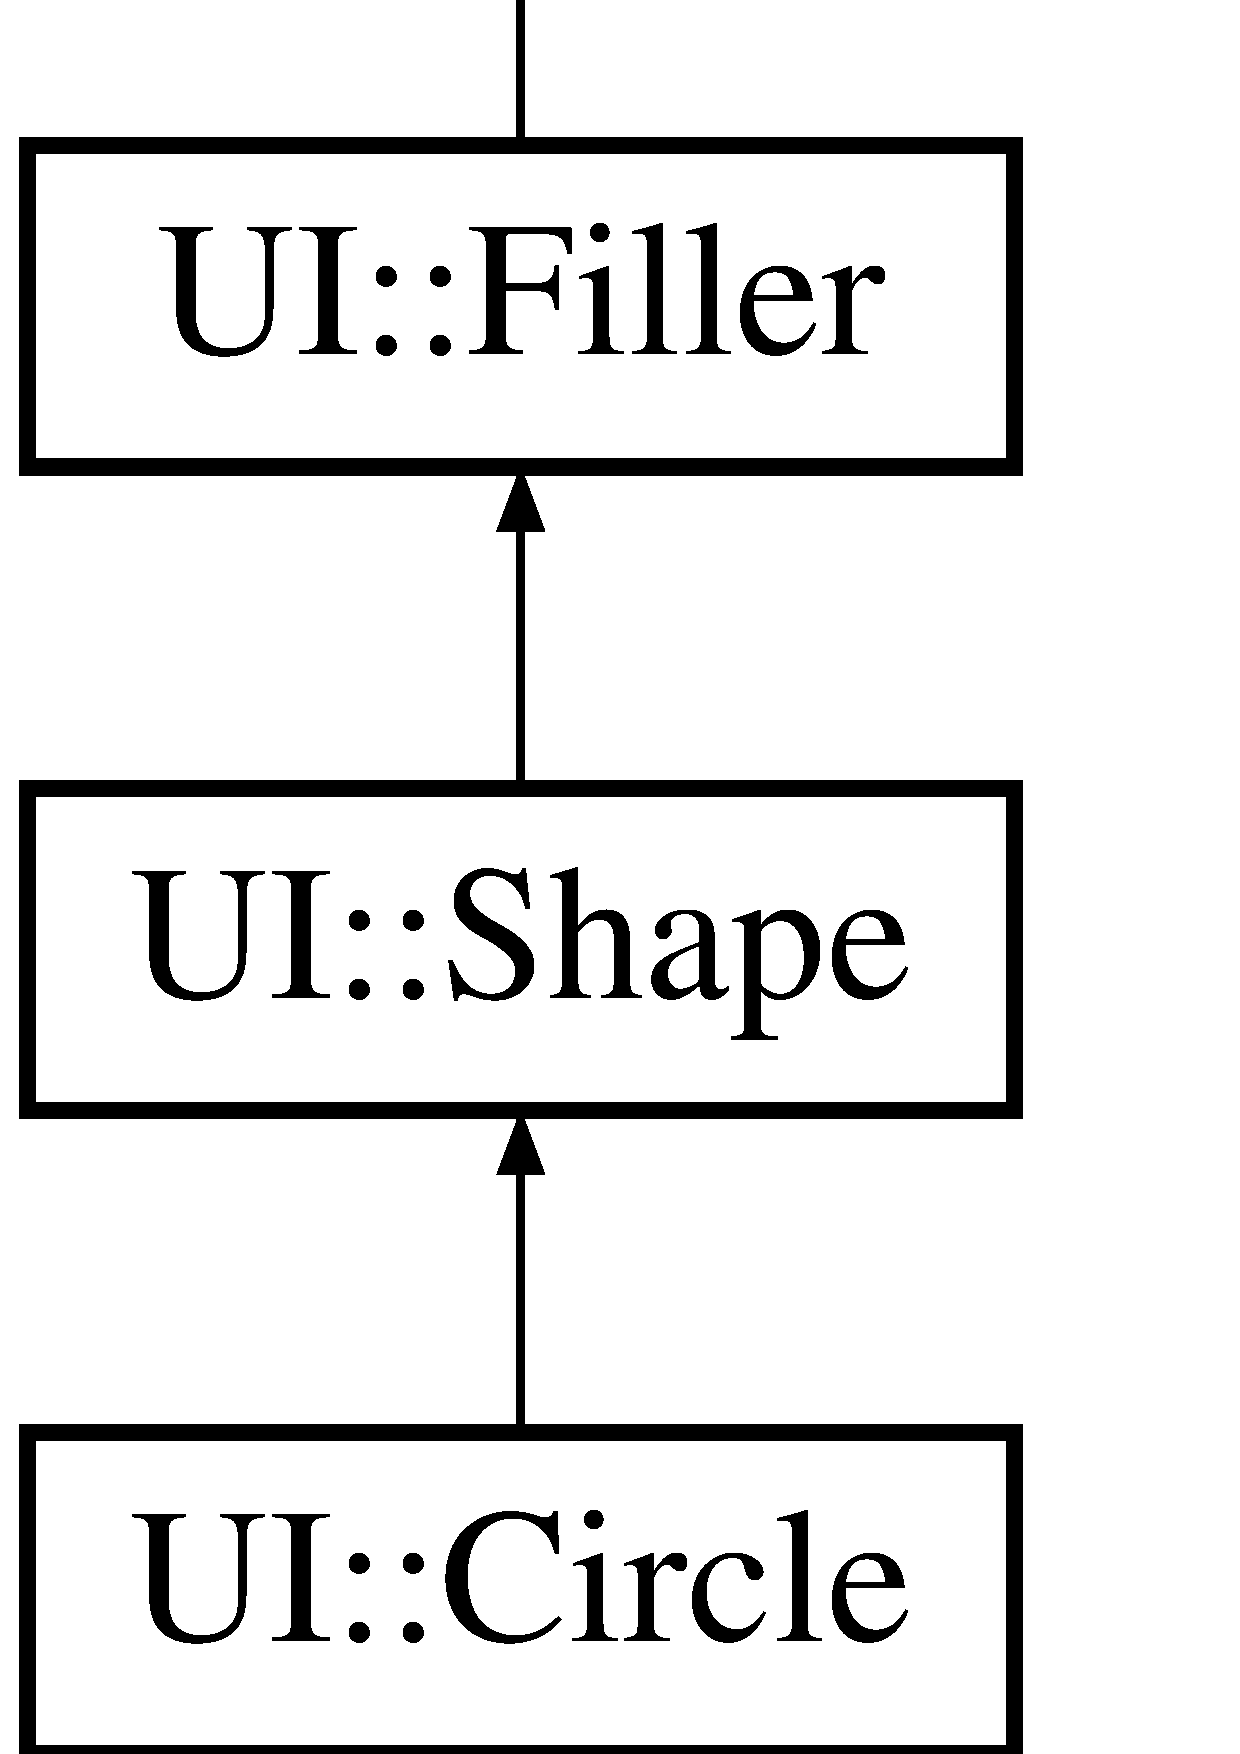
\includegraphics[height=4.000000cm]{struct_u_i_1_1_circle}
\end{center}
\end{figure}
\subsection*{Public Member Functions}
\begin{DoxyCompactItemize}
\item 
\mbox{\Hypertarget{struct_u_i_1_1_circle_a5600f155916282d150f5001dc4eee7bf}\label{struct_u_i_1_1_circle_a5600f155916282d150f5001dc4eee7bf}} 
void {\bfseries setup} (const \hyperlink{struct_u_i_1_1_color}{Color} \&color\+\_\+, float size, int type\+\_\+=S\+O\+L\+ID)
\item 
\mbox{\Hypertarget{struct_u_i_1_1_circle_a992cb6f90c9e5d847385ccc0dce4feeb}\label{struct_u_i_1_1_circle_a992cb6f90c9e5d847385ccc0dce4feeb}} 
const char $\ast$ {\bfseries gettype} () const
\item 
\mbox{\Hypertarget{struct_u_i_1_1_circle_a3b333027c89114c07bf84110b3999502}\label{struct_u_i_1_1_circle_a3b333027c89114c07bf84110b3999502}} 
bool {\bfseries target} (float cx, float cy)
\item 
\mbox{\Hypertarget{struct_u_i_1_1_circle_abcc7f2fb85dbae67eec9cc5cf8943a50}\label{struct_u_i_1_1_circle_abcc7f2fb85dbae67eec9cc5cf8943a50}} 
void {\bfseries draw} (float sx, float sy)
\end{DoxyCompactItemize}
\subsection*{Static Public Member Functions}
\begin{DoxyCompactItemize}
\item 
\mbox{\Hypertarget{struct_u_i_1_1_circle_a01fcff8f643bfc84135d449d01317868}\label{struct_u_i_1_1_circle_a01fcff8f643bfc84135d449d01317868}} 
static const char $\ast$ {\bfseries typestr} ()
\end{DoxyCompactItemize}
\subsection*{Public Attributes}
\begin{DoxyCompactItemize}
\item 
\mbox{\Hypertarget{struct_u_i_1_1_circle_a0361e309f2ad61fee6a4a7bd07d2a690}\label{struct_u_i_1_1_circle_a0361e309f2ad61fee6a4a7bd07d2a690}} 
float {\bfseries radius}
\end{DoxyCompactItemize}
\subsection*{Additional Inherited Members}


The documentation for this struct was generated from the following file\+:\begin{DoxyCompactItemize}
\item 
H\+:/\+Rival\+Engine/\+Rival\+\_\+\+Game\+\_\+\+Engine\+\_\+\+G\+I\+T/\+Rival3dengine/source/engine/ui.\+cpp\end{DoxyCompactItemize}

\hypertarget{structclient}{}\section{client Struct Reference}
\label{structclient}\index{client@{client}}
\subsection*{Public Attributes}
\begin{DoxyCompactItemize}
\item 
\mbox{\Hypertarget{structclient_ac73e88565012803f65fc5b5f2be32252}\label{structclient_ac73e88565012803f65fc5b5f2be32252}} 
E\+Net\+Address {\bfseries address}
\item 
\mbox{\Hypertarget{structclient_a636ca58d7fe24e2aa0106b1c5da903e0}\label{structclient_a636ca58d7fe24e2aa0106b1c5da903e0}} 
E\+Net\+Socket {\bfseries socket}
\item 
\mbox{\Hypertarget{structclient_a83b3ee389e5166fa852db052d50dabdf}\label{structclient_a83b3ee389e5166fa852db052d50dabdf}} 
char {\bfseries input} \mbox{[}I\+N\+P\+U\+T\+\_\+\+L\+I\+M\+IT\mbox{]}
\item 
\mbox{\Hypertarget{structclient_ad4247c8cc8cc217f535f93e581f100f5}\label{structclient_ad4247c8cc8cc217f535f93e581f100f5}} 
\hyperlink{structmessagebuf}{messagebuf} $\ast$ {\bfseries message}
\item 
\mbox{\Hypertarget{structclient_a3f85a35a8b007d5b89821f9219ed13a0}\label{structclient_a3f85a35a8b007d5b89821f9219ed13a0}} 
\hyperlink{structvector}{vector}$<$ char $>$ {\bfseries output}
\item 
\mbox{\Hypertarget{structclient_a9edfa1f7885780b718dfa5d57f6b368b}\label{structclient_a9edfa1f7885780b718dfa5d57f6b368b}} 
int {\bfseries inputpos}
\item 
\mbox{\Hypertarget{structclient_ae714dd677ac44a935a603a4f918bd06e}\label{structclient_ae714dd677ac44a935a603a4f918bd06e}} 
int {\bfseries outputpos}
\item 
\mbox{\Hypertarget{structclient_a6a61070ed4219f32678394384754ed5d}\label{structclient_a6a61070ed4219f32678394384754ed5d}} 
enet\+\_\+uint32 {\bfseries connecttime}
\item 
\mbox{\Hypertarget{structclient_a89cf74f72fc6beee69f75f81d4ab959f}\label{structclient_a89cf74f72fc6beee69f75f81d4ab959f}} 
enet\+\_\+uint32 {\bfseries lastinput}
\item 
\mbox{\Hypertarget{structclient_a9e9f7389b4d687a0b8151a0eeb13ed48}\label{structclient_a9e9f7389b4d687a0b8151a0eeb13ed48}} 
int {\bfseries servport}
\item 
\mbox{\Hypertarget{structclient_a96ab158e5da6a1c4b4d91bd2156d69a6}\label{structclient_a96ab158e5da6a1c4b4d91bd2156d69a6}} 
enet\+\_\+uint32 {\bfseries lastauth}
\item 
\mbox{\Hypertarget{structclient_ac5cce599724c2ae9afece3647cc61c77}\label{structclient_ac5cce599724c2ae9afece3647cc61c77}} 
\hyperlink{structvector}{vector}$<$ \hyperlink{structauthreq}{authreq} $>$ {\bfseries authreqs}
\item 
\mbox{\Hypertarget{structclient_a82b12351d4d3f132dc6ddb9f3c460014}\label{structclient_a82b12351d4d3f132dc6ddb9f3c460014}} 
bool {\bfseries shouldpurge}
\item 
\mbox{\Hypertarget{structclient_a87b66536569f8a87a3ecb798f89fd01d}\label{structclient_a87b66536569f8a87a3ecb798f89fd01d}} 
bool {\bfseries registeredserver}
\item 
\mbox{\Hypertarget{structclient_a52bb4f1e5551cc4e6a5bac9b6b10a421}\label{structclient_a52bb4f1e5551cc4e6a5bac9b6b10a421}} 
int {\bfseries type}
\item 
\mbox{\Hypertarget{structclient_ad5bc3dbea459c9c274cf33e92411bd63}\label{structclient_ad5bc3dbea459c9c274cf33e92411bd63}} 
int {\bfseries num}
\item 
\mbox{\Hypertarget{structclient_a909db3ee6d690070a7b3bb84f85ca55d}\label{structclient_a909db3ee6d690070a7b3bb84f85ca55d}} 
E\+Net\+Peer $\ast$ {\bfseries peer}
\item 
\mbox{\Hypertarget{structclient_abc6088526d5f9b920c5445f005244175}\label{structclient_abc6088526d5f9b920c5445f005244175}} 
cubestr {\bfseries hostname}
\item 
\mbox{\Hypertarget{structclient_a565e30169a6d838e27ae4ced2490e755}\label{structclient_a565e30169a6d838e27ae4ced2490e755}} 
void $\ast$ {\bfseries info}
\end{DoxyCompactItemize}


The documentation for this struct was generated from the following files\+:\begin{DoxyCompactItemize}
\item 
H\+:/\+Rival\+Engine/\+Rival\+\_\+\+Game\+\_\+\+Engine\+\_\+\+G\+I\+T/\+Rival3dengine/source/engine/master.\+cpp\item 
H\+:/\+Rival\+Engine/\+Rival\+\_\+\+Game\+\_\+\+Engine\+\_\+\+G\+I\+T/\+Rival3dengine/source/engine/server.\+cpp\end{DoxyCompactItemize}

\hypertarget{structserver_1_1clientinfo}{}\section{server\+:\+:clientinfo Struct Reference}
\label{structserver_1_1clientinfo}\index{server\+::clientinfo@{server\+::clientinfo}}
\subsection*{Public Types}
\begin{DoxyCompactItemize}
\item 
\mbox{\Hypertarget{structserver_1_1clientinfo_ad6da0c29adb5ee59f89caf401b430790}\label{structserver_1_1clientinfo_ad6da0c29adb5ee59f89caf401b430790}} 
enum \{ {\bfseries P\+U\+S\+H\+M\+I\+L\+L\+IS} = 3000
 \}
\end{DoxyCompactItemize}
\subsection*{Public Member Functions}
\begin{DoxyCompactItemize}
\item 
\mbox{\Hypertarget{structserver_1_1clientinfo_a38a1bf4febbe675f44ee31224f746ff6}\label{structserver_1_1clientinfo_a38a1bf4febbe675f44ee31224f746ff6}} 
void {\bfseries addevent} (\hyperlink{structserver_1_1gameevent}{gameevent} $\ast$e)
\item 
\mbox{\Hypertarget{structserver_1_1clientinfo_a2466cde18027b1da1e0034c8d12d2c62}\label{structserver_1_1clientinfo_a2466cde18027b1da1e0034c8d12d2c62}} 
int {\bfseries calcpushrange} ()
\item 
\mbox{\Hypertarget{structserver_1_1clientinfo_a334e58d4f2f0698cbbd087c5a9a73cef}\label{structserver_1_1clientinfo_a334e58d4f2f0698cbbd087c5a9a73cef}} 
bool {\bfseries checkpushed} (int millis, int range)
\item 
\mbox{\Hypertarget{structserver_1_1clientinfo_af0e88f0a6b326d2199ec21809365b3ca}\label{structserver_1_1clientinfo_af0e88f0a6b326d2199ec21809365b3ca}} 
void {\bfseries scheduleexceeded} ()
\item 
\mbox{\Hypertarget{structserver_1_1clientinfo_ab1aafce1865c46d1cdece4434a6628db}\label{structserver_1_1clientinfo_ab1aafce1865c46d1cdece4434a6628db}} 
void {\bfseries setexceeded} ()
\item 
\mbox{\Hypertarget{structserver_1_1clientinfo_af77ef8d33e9be42088687e0e998d6f35}\label{structserver_1_1clientinfo_af77ef8d33e9be42088687e0e998d6f35}} 
void {\bfseries setpushed} ()
\item 
\mbox{\Hypertarget{structserver_1_1clientinfo_a7871e865162abe6c0c708cefa90524d7}\label{structserver_1_1clientinfo_a7871e865162abe6c0c708cefa90524d7}} 
bool {\bfseries checkexceeded} ()
\item 
\mbox{\Hypertarget{structserver_1_1clientinfo_a1d6ac1b1bb4bbf48669d88791c4794d5}\label{structserver_1_1clientinfo_a1d6ac1b1bb4bbf48669d88791c4794d5}} 
void {\bfseries mapchange} ()
\item 
\mbox{\Hypertarget{structserver_1_1clientinfo_ac4745359622a834ee79bd8dcbd757546}\label{structserver_1_1clientinfo_ac4745359622a834ee79bd8dcbd757546}} 
void {\bfseries reassign} ()
\item 
\mbox{\Hypertarget{structserver_1_1clientinfo_a801db6eb4ec0397d275f4e09be79569c}\label{structserver_1_1clientinfo_a801db6eb4ec0397d275f4e09be79569c}} 
void {\bfseries cleanclipboard} (bool fullclean=true)
\item 
\mbox{\Hypertarget{structserver_1_1clientinfo_ae385924a6d99e68bd6b4550c50713b12}\label{structserver_1_1clientinfo_ae385924a6d99e68bd6b4550c50713b12}} 
void {\bfseries cleanauthkick} ()
\item 
\mbox{\Hypertarget{structserver_1_1clientinfo_a83892c395c493c8fe9a931e0a0b0440c}\label{structserver_1_1clientinfo_a83892c395c493c8fe9a931e0a0b0440c}} 
void {\bfseries cleanauth} (bool full=true)
\item 
\mbox{\Hypertarget{structserver_1_1clientinfo_a0c423be136e2ca972f4b13b053c0823d}\label{structserver_1_1clientinfo_a0c423be136e2ca972f4b13b053c0823d}} 
void {\bfseries reset} ()
\item 
\mbox{\Hypertarget{structserver_1_1clientinfo_a33ed0f9aab1ca3a28738b760fd68f583}\label{structserver_1_1clientinfo_a33ed0f9aab1ca3a28738b760fd68f583}} 
int {\bfseries geteventmillis} (int servmillis, int clientmillis)
\end{DoxyCompactItemize}
\subsection*{Public Attributes}
\begin{DoxyCompactItemize}
\item 
\mbox{\Hypertarget{structserver_1_1clientinfo_a3ecc5031c20160ed0b72324d07a371a5}\label{structserver_1_1clientinfo_a3ecc5031c20160ed0b72324d07a371a5}} 
int {\bfseries clientnum}
\item 
\mbox{\Hypertarget{structserver_1_1clientinfo_aa803b3ecd777f7e83153e1d4b83f1a10}\label{structserver_1_1clientinfo_aa803b3ecd777f7e83153e1d4b83f1a10}} 
int {\bfseries ownernum}
\item 
\mbox{\Hypertarget{structserver_1_1clientinfo_afb3498182d64f6a2e86e0dcd835d17df}\label{structserver_1_1clientinfo_afb3498182d64f6a2e86e0dcd835d17df}} 
int {\bfseries connectmillis}
\item 
\mbox{\Hypertarget{structserver_1_1clientinfo_a0b45abd9fb3f85e5e0ff62b86f1ddfa4}\label{structserver_1_1clientinfo_a0b45abd9fb3f85e5e0ff62b86f1ddfa4}} 
int {\bfseries sessionid}
\item 
\mbox{\Hypertarget{structserver_1_1clientinfo_afdb907491d4453ec7634b63f78e77d5c}\label{structserver_1_1clientinfo_afdb907491d4453ec7634b63f78e77d5c}} 
int {\bfseries overflow}
\item 
\mbox{\Hypertarget{structserver_1_1clientinfo_afdcfc91a4e7ff892fe2afb9e1e7c8e05}\label{structserver_1_1clientinfo_afdcfc91a4e7ff892fe2afb9e1e7c8e05}} 
cubestr {\bfseries name}
\item 
\mbox{\Hypertarget{structserver_1_1clientinfo_a8959f2299efb82796751be391d1a372c}\label{structserver_1_1clientinfo_a8959f2299efb82796751be391d1a372c}} 
cubestr {\bfseries mapvote}
\item 
\mbox{\Hypertarget{structserver_1_1clientinfo_a278efa351776a339538d904f2aea05f6}\label{structserver_1_1clientinfo_a278efa351776a339538d904f2aea05f6}} 
int {\bfseries team}
\item 
\mbox{\Hypertarget{structserver_1_1clientinfo_affdbed069334fe3811cde2f02e5d842e}\label{structserver_1_1clientinfo_affdbed069334fe3811cde2f02e5d842e}} 
int {\bfseries playermodel}
\item 
\mbox{\Hypertarget{structserver_1_1clientinfo_a7f3a6ac80a4decd6902e2a567a017917}\label{structserver_1_1clientinfo_a7f3a6ac80a4decd6902e2a567a017917}} 
int {\bfseries playercolor}
\item 
\mbox{\Hypertarget{structserver_1_1clientinfo_ace1c7964d3d41ae6ce0a3869ececc586}\label{structserver_1_1clientinfo_ace1c7964d3d41ae6ce0a3869ececc586}} 
int {\bfseries modevote}
\item 
\mbox{\Hypertarget{structserver_1_1clientinfo_a8773b9cb88b5d7c5a5185cac05630847}\label{structserver_1_1clientinfo_a8773b9cb88b5d7c5a5185cac05630847}} 
int {\bfseries privilege}
\item 
\mbox{\Hypertarget{structserver_1_1clientinfo_accc64cfb12e5c816af25f3c568a5b2d4}\label{structserver_1_1clientinfo_accc64cfb12e5c816af25f3c568a5b2d4}} 
bool {\bfseries connected}
\item 
\mbox{\Hypertarget{structserver_1_1clientinfo_a15acb839659009482c46e15eaef5a62f}\label{structserver_1_1clientinfo_a15acb839659009482c46e15eaef5a62f}} 
bool {\bfseries local}
\item 
\mbox{\Hypertarget{structserver_1_1clientinfo_a8be92879ff4f263d3e0bc499c283fc7b}\label{structserver_1_1clientinfo_a8be92879ff4f263d3e0bc499c283fc7b}} 
bool {\bfseries timesync}
\item 
\mbox{\Hypertarget{structserver_1_1clientinfo_a49833d3ccda00e0aca0ed11572b7d4c1}\label{structserver_1_1clientinfo_a49833d3ccda00e0aca0ed11572b7d4c1}} 
int {\bfseries gameoffset}
\item 
\mbox{\Hypertarget{structserver_1_1clientinfo_a5478b64f83ca1725ffb3d89ce10e1fd6}\label{structserver_1_1clientinfo_a5478b64f83ca1725ffb3d89ce10e1fd6}} 
int {\bfseries lastevent}
\item 
\mbox{\Hypertarget{structserver_1_1clientinfo_a6ddd8bd687906f18b8c7215b653d08ca}\label{structserver_1_1clientinfo_a6ddd8bd687906f18b8c7215b653d08ca}} 
int {\bfseries pushed}
\item 
\mbox{\Hypertarget{structserver_1_1clientinfo_a11894e094e882ce0097ddfd4d60a4390}\label{structserver_1_1clientinfo_a11894e094e882ce0097ddfd4d60a4390}} 
int {\bfseries exceeded}
\item 
\mbox{\Hypertarget{structserver_1_1clientinfo_ae09ebbc2d6b3b329fa600444c88d0526}\label{structserver_1_1clientinfo_ae09ebbc2d6b3b329fa600444c88d0526}} 
\hyperlink{structserver_1_1servstate}{servstate} {\bfseries state}
\item 
\mbox{\Hypertarget{structserver_1_1clientinfo_a7da3c16a57016e0ddbee344a92e9576e}\label{structserver_1_1clientinfo_a7da3c16a57016e0ddbee344a92e9576e}} 
\hyperlink{structvector}{vector}$<$ \hyperlink{structserver_1_1gameevent}{gameevent} $\ast$ $>$ {\bfseries events}
\item 
\mbox{\Hypertarget{structserver_1_1clientinfo_af6c6d82d90bc2cc66158e9a162b353cc}\label{structserver_1_1clientinfo_af6c6d82d90bc2cc66158e9a162b353cc}} 
\hyperlink{structvector}{vector}$<$ uchar $>$ {\bfseries position}
\item 
\mbox{\Hypertarget{structserver_1_1clientinfo_ac935533746dc0e88c5cb8ab44cc99167}\label{structserver_1_1clientinfo_ac935533746dc0e88c5cb8ab44cc99167}} 
\hyperlink{structvector}{vector}$<$ uchar $>$ {\bfseries messages}
\item 
\mbox{\Hypertarget{structserver_1_1clientinfo_ad2a4c6d2bba1d0d05451b6a046f0cf51}\label{structserver_1_1clientinfo_ad2a4c6d2bba1d0d05451b6a046f0cf51}} 
uchar $\ast$ {\bfseries wsdata}
\item 
\mbox{\Hypertarget{structserver_1_1clientinfo_af187ed2b9e2f7702cff33db3e6e741ef}\label{structserver_1_1clientinfo_af187ed2b9e2f7702cff33db3e6e741ef}} 
int {\bfseries wslen}
\item 
\mbox{\Hypertarget{structserver_1_1clientinfo_a87ba878f713289a84864bf32a5cf55f9}\label{structserver_1_1clientinfo_a87ba878f713289a84864bf32a5cf55f9}} 
\hyperlink{structvector}{vector}$<$ \hyperlink{structserver_1_1clientinfo}{clientinfo} $\ast$ $>$ {\bfseries bots}
\item 
\mbox{\Hypertarget{structserver_1_1clientinfo_a191fa2fea779563d9a090b2ea88f0845}\label{structserver_1_1clientinfo_a191fa2fea779563d9a090b2ea88f0845}} 
int {\bfseries ping}
\item 
\mbox{\Hypertarget{structserver_1_1clientinfo_af92725649c7a594e1b1fad2bf655e2b8}\label{structserver_1_1clientinfo_af92725649c7a594e1b1fad2bf655e2b8}} 
int {\bfseries aireinit}
\item 
\mbox{\Hypertarget{structserver_1_1clientinfo_a469bd680490aced6200475132c12789f}\label{structserver_1_1clientinfo_a469bd680490aced6200475132c12789f}} 
cubestr {\bfseries clientmap}
\item 
\mbox{\Hypertarget{structserver_1_1clientinfo_a1b906701a66ca6c2dcb0ac2a8dc102fd}\label{structserver_1_1clientinfo_a1b906701a66ca6c2dcb0ac2a8dc102fd}} 
int {\bfseries mapcrc}
\item 
\mbox{\Hypertarget{structserver_1_1clientinfo_a390fd938f9ce2f31303266a6cc0e2dc6}\label{structserver_1_1clientinfo_a390fd938f9ce2f31303266a6cc0e2dc6}} 
bool {\bfseries warned}
\item 
\mbox{\Hypertarget{structserver_1_1clientinfo_a51d591008d2698bcec88759f7520ea54}\label{structserver_1_1clientinfo_a51d591008d2698bcec88759f7520ea54}} 
bool {\bfseries gameclip}
\item 
\mbox{\Hypertarget{structserver_1_1clientinfo_a106d722fa0c5c056a37bdcbfa7021705}\label{structserver_1_1clientinfo_a106d722fa0c5c056a37bdcbfa7021705}} 
E\+Net\+Packet $\ast$ {\bfseries getdemo}
\item 
\mbox{\Hypertarget{structserver_1_1clientinfo_afe90c90631889918528cd92efca6bd74}\label{structserver_1_1clientinfo_afe90c90631889918528cd92efca6bd74}} 
E\+Net\+Packet $\ast$ {\bfseries getmap}
\item 
\mbox{\Hypertarget{structserver_1_1clientinfo_a9b361c429e68884cde9c7489af43e366}\label{structserver_1_1clientinfo_a9b361c429e68884cde9c7489af43e366}} 
E\+Net\+Packet $\ast$ {\bfseries clipboard}
\item 
\mbox{\Hypertarget{structserver_1_1clientinfo_a3250512af682e86a507d65767cccdb33}\label{structserver_1_1clientinfo_a3250512af682e86a507d65767cccdb33}} 
int {\bfseries lastclipboard}
\item 
\mbox{\Hypertarget{structserver_1_1clientinfo_ab8a50a8d6060a012441eb5e265179a73}\label{structserver_1_1clientinfo_ab8a50a8d6060a012441eb5e265179a73}} 
int {\bfseries needclipboard}
\item 
\mbox{\Hypertarget{structserver_1_1clientinfo_ae9bf281b7742705a23ffec8cbc67e290}\label{structserver_1_1clientinfo_ae9bf281b7742705a23ffec8cbc67e290}} 
int {\bfseries connectauth}
\item 
\mbox{\Hypertarget{structserver_1_1clientinfo_a5acab1da73faeaab8661d660f8440e29}\label{structserver_1_1clientinfo_a5acab1da73faeaab8661d660f8440e29}} 
uint {\bfseries authreq}
\item 
\mbox{\Hypertarget{structserver_1_1clientinfo_ad53b41b38baa0fbdd93e135c88c3a348}\label{structserver_1_1clientinfo_ad53b41b38baa0fbdd93e135c88c3a348}} 
cubestr {\bfseries authname}
\item 
\mbox{\Hypertarget{structserver_1_1clientinfo_ae424791dd7324173d9599ad4e7a47fe6}\label{structserver_1_1clientinfo_ae424791dd7324173d9599ad4e7a47fe6}} 
cubestr {\bfseries authdesc}
\item 
\mbox{\Hypertarget{structserver_1_1clientinfo_adfbba599ef870c7abab914b5a8bfa4a5}\label{structserver_1_1clientinfo_adfbba599ef870c7abab914b5a8bfa4a5}} 
void $\ast$ {\bfseries authchallenge}
\item 
\mbox{\Hypertarget{structserver_1_1clientinfo_a7328f0d7bb6dd93df11a82ab864be89a}\label{structserver_1_1clientinfo_a7328f0d7bb6dd93df11a82ab864be89a}} 
int {\bfseries authkickvictim}
\item 
\mbox{\Hypertarget{structserver_1_1clientinfo_a74b689c598a29ac26e9a8535cf9fd7cb}\label{structserver_1_1clientinfo_a74b689c598a29ac26e9a8535cf9fd7cb}} 
char $\ast$ {\bfseries authkickreason}
\end{DoxyCompactItemize}


The documentation for this struct was generated from the following file\+:\begin{DoxyCompactItemize}
\item 
H\+:/\+Rival\+Engine/\+Rival\+\_\+\+Game\+\_\+\+Engine\+\_\+\+G\+I\+T/\+Rival3dengine/source/game/server.\+cpp\end{DoxyCompactItemize}

\hypertarget{structgame_1_1clientmode}{}\section{game\+:\+:clientmode Struct Reference}
\label{structgame_1_1clientmode}\index{game\+::clientmode@{game\+::clientmode}}
Inheritance diagram for game\+:\+:clientmode\+:\begin{figure}[H]
\begin{center}
\leavevmode
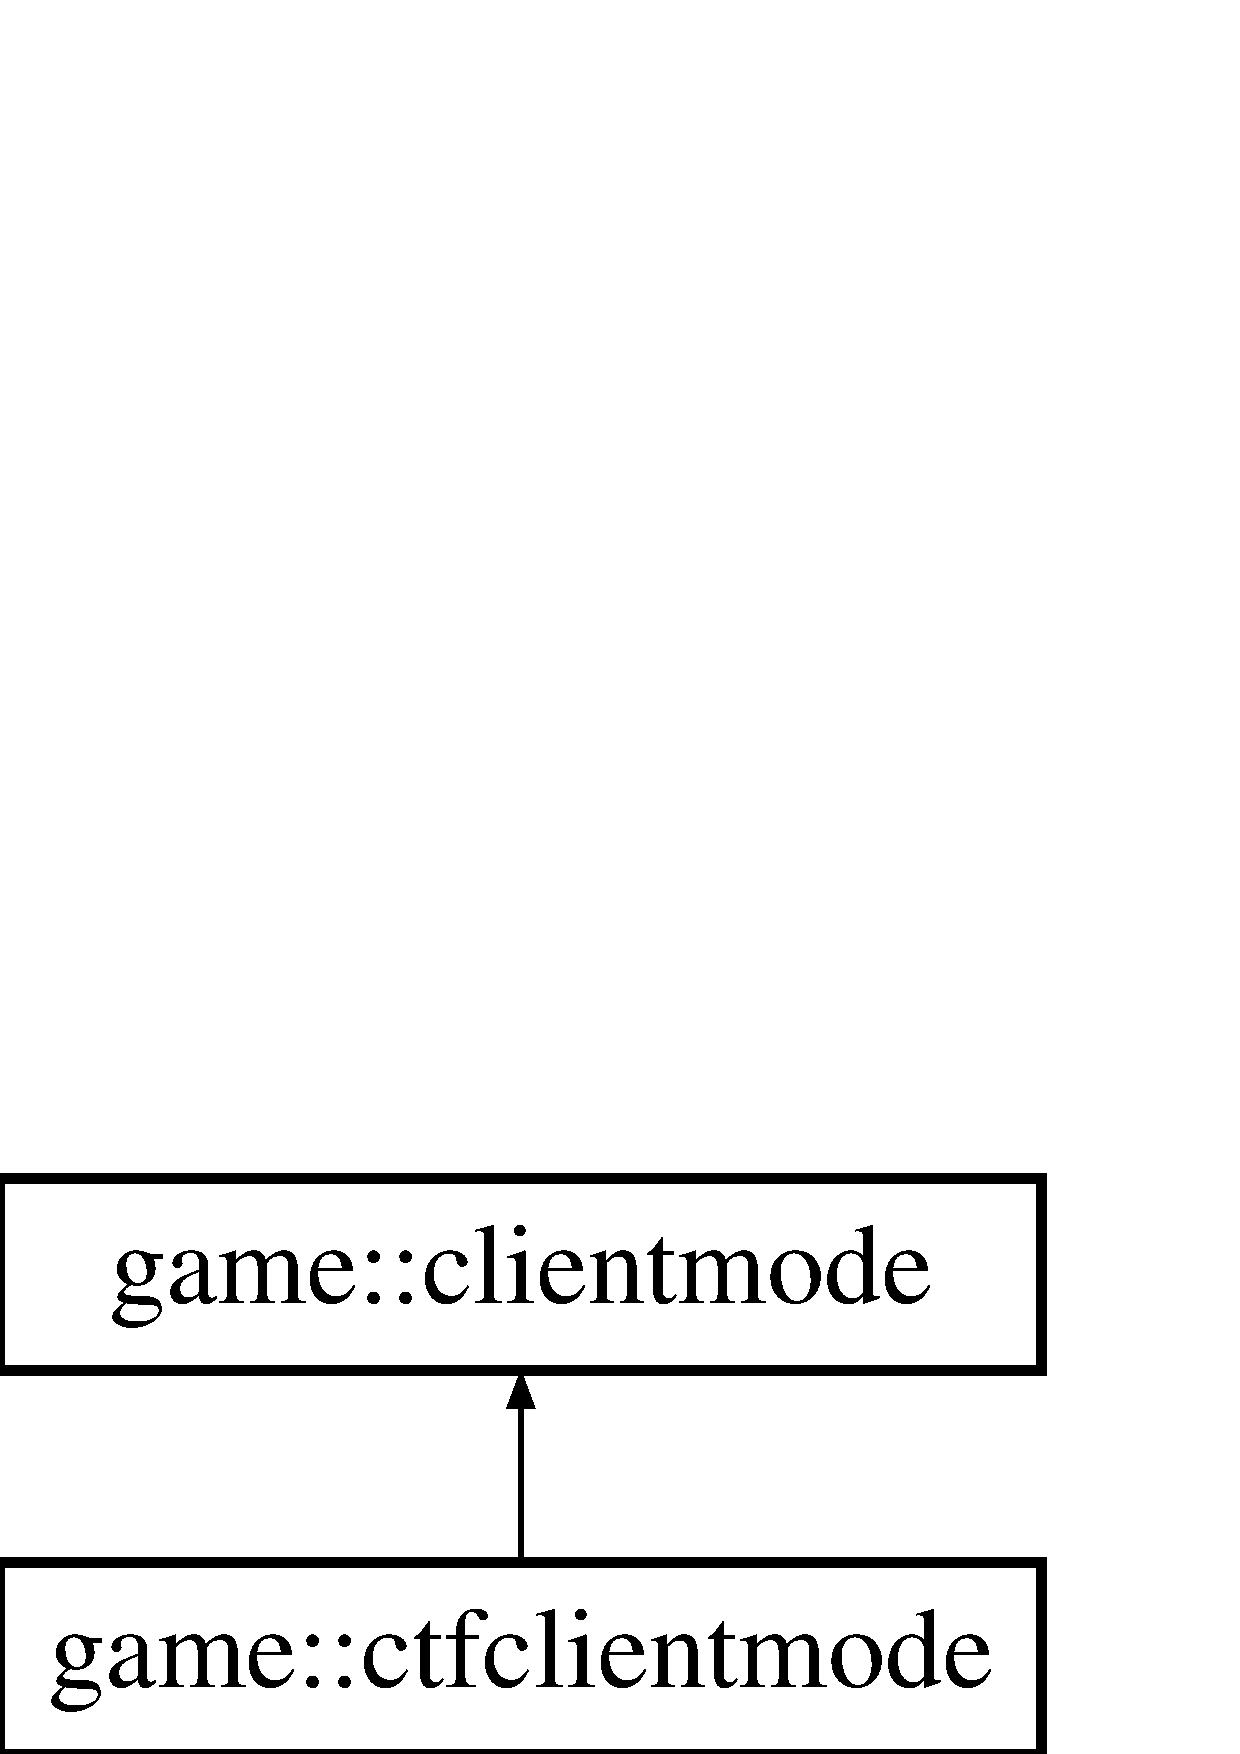
\includegraphics[height=2.000000cm]{structgame_1_1clientmode}
\end{center}
\end{figure}
\subsection*{Public Member Functions}
\begin{DoxyCompactItemize}
\item 
\mbox{\Hypertarget{structgame_1_1clientmode_a1beb9f371902517ea005c1ba3e3f27c2}\label{structgame_1_1clientmode_a1beb9f371902517ea005c1ba3e3f27c2}} 
virtual void {\bfseries preload} ()
\item 
\mbox{\Hypertarget{structgame_1_1clientmode_a0af55e985aafec5574fb8a5d85ccad7b}\label{structgame_1_1clientmode_a0af55e985aafec5574fb8a5d85ccad7b}} 
virtual float {\bfseries clipconsole} (float w, float h)
\item 
\mbox{\Hypertarget{structgame_1_1clientmode_a3853a921a65e26d3d5191dbb6dcbaf27}\label{structgame_1_1clientmode_a3853a921a65e26d3d5191dbb6dcbaf27}} 
virtual void {\bfseries drawhud} (\hyperlink{structgameent}{gameent} $\ast$d, int w, int h)
\item 
\mbox{\Hypertarget{structgame_1_1clientmode_a78c5605c83809da8eff961ff8e8c276f}\label{structgame_1_1clientmode_a78c5605c83809da8eff961ff8e8c276f}} 
virtual void {\bfseries rendergame} ()
\item 
\mbox{\Hypertarget{structgame_1_1clientmode_a694580c6c480d4c365f4654c699fb305}\label{structgame_1_1clientmode_a694580c6c480d4c365f4654c699fb305}} 
virtual void {\bfseries respawned} (\hyperlink{structgameent}{gameent} $\ast$d)
\item 
\mbox{\Hypertarget{structgame_1_1clientmode_a44fc841a183a5beb3838fc8cb62f2144}\label{structgame_1_1clientmode_a44fc841a183a5beb3838fc8cb62f2144}} 
virtual void {\bfseries setup} ()
\item 
\mbox{\Hypertarget{structgame_1_1clientmode_a0fb8b920d580627cc9f7c91aa612a0be}\label{structgame_1_1clientmode_a0fb8b920d580627cc9f7c91aa612a0be}} 
virtual void {\bfseries checkitems} (\hyperlink{structgameent}{gameent} $\ast$d)
\item 
\mbox{\Hypertarget{structgame_1_1clientmode_ab79774790886c3e75b2611240a482a25}\label{structgame_1_1clientmode_ab79774790886c3e75b2611240a482a25}} 
virtual int {\bfseries respawnwait} (\hyperlink{structgameent}{gameent} $\ast$d)
\item 
\mbox{\Hypertarget{structgame_1_1clientmode_a615c81ca9082838a15d1d57716c1f056}\label{structgame_1_1clientmode_a615c81ca9082838a15d1d57716c1f056}} 
virtual void {\bfseries pickspawn} (\hyperlink{structgameent}{gameent} $\ast$d)
\item 
\mbox{\Hypertarget{structgame_1_1clientmode_af911531e1533abc04313785b874080e2}\label{structgame_1_1clientmode_af911531e1533abc04313785b874080e2}} 
virtual void {\bfseries senditems} (\hyperlink{structpacketbuf}{packetbuf} \&p)
\item 
\mbox{\Hypertarget{structgame_1_1clientmode_ab84ceae05f9c8b687c657722e1ca1f26}\label{structgame_1_1clientmode_ab84ceae05f9c8b687c657722e1ca1f26}} 
virtual void {\bfseries removeplayer} (\hyperlink{structgameent}{gameent} $\ast$d)
\item 
\mbox{\Hypertarget{structgame_1_1clientmode_ad196dd3c0f9e609a5282c94b903d45ef}\label{structgame_1_1clientmode_ad196dd3c0f9e609a5282c94b903d45ef}} 
virtual void {\bfseries gameover} ()
\item 
\mbox{\Hypertarget{structgame_1_1clientmode_a1f1ef26efdef70b0976a99a5ad794b46}\label{structgame_1_1clientmode_a1f1ef26efdef70b0976a99a5ad794b46}} 
virtual bool {\bfseries hidefrags} ()
\item 
\mbox{\Hypertarget{structgame_1_1clientmode_aea5be25100da67d8263b0e144e324c64}\label{structgame_1_1clientmode_aea5be25100da67d8263b0e144e324c64}} 
virtual int {\bfseries getteamscore} (int team)
\item 
\mbox{\Hypertarget{structgame_1_1clientmode_afa7b0f23e0ac3446da71e3c90bb2fd46}\label{structgame_1_1clientmode_afa7b0f23e0ac3446da71e3c90bb2fd46}} 
virtual void {\bfseries getteamscores} (\hyperlink{structvector}{vector}$<$ \hyperlink{structteamscore}{teamscore} $>$ \&scores)
\item 
\mbox{\Hypertarget{structgame_1_1clientmode_a1efc58a0529fc0f54482034fe88a4349}\label{structgame_1_1clientmode_a1efc58a0529fc0f54482034fe88a4349}} 
virtual void {\bfseries aifind} (\hyperlink{structgameent}{gameent} $\ast$d, \hyperlink{structai_1_1aistate}{ai\+::aistate} \&b, \hyperlink{structvector}{vector}$<$ \hyperlink{structai_1_1interest}{ai\+::interest} $>$ \&interests)
\item 
\mbox{\Hypertarget{structgame_1_1clientmode_a7782032ba1254d274b29411769e4a9f8}\label{structgame_1_1clientmode_a7782032ba1254d274b29411769e4a9f8}} 
virtual bool {\bfseries aicheck} (\hyperlink{structgameent}{gameent} $\ast$d, \hyperlink{structai_1_1aistate}{ai\+::aistate} \&b)
\item 
\mbox{\Hypertarget{structgame_1_1clientmode_a342fdb830ecf89adc4751a7a3dceac75}\label{structgame_1_1clientmode_a342fdb830ecf89adc4751a7a3dceac75}} 
virtual bool {\bfseries aidefend} (\hyperlink{structgameent}{gameent} $\ast$d, \hyperlink{structai_1_1aistate}{ai\+::aistate} \&b)
\item 
\mbox{\Hypertarget{structgame_1_1clientmode_a1712443b96d442fe69afc076d0476561}\label{structgame_1_1clientmode_a1712443b96d442fe69afc076d0476561}} 
virtual bool {\bfseries aipursue} (\hyperlink{structgameent}{gameent} $\ast$d, \hyperlink{structai_1_1aistate}{ai\+::aistate} \&b)
\end{DoxyCompactItemize}


The documentation for this struct was generated from the following file\+:\begin{DoxyCompactItemize}
\item 
H\+:/\+Rival\+Engine/\+Rival\+\_\+\+Game\+\_\+\+Engine\+\_\+\+G\+I\+T/\+Rival3dengine/source/game/game.\+h\end{DoxyCompactItemize}

\hypertarget{structcline}{}\section{cline Struct Reference}
\label{structcline}\index{cline@{cline}}
\subsection*{Public Attributes}
\begin{DoxyCompactItemize}
\item 
\mbox{\Hypertarget{structcline_a6693eaa3be2233cab8b591dbe50bc88b}\label{structcline_a6693eaa3be2233cab8b591dbe50bc88b}} 
char $\ast$ {\bfseries line}
\item 
\mbox{\Hypertarget{structcline_aad264f8b9b2cc3e83d5fcd4c6fe77c8e}\label{structcline_aad264f8b9b2cc3e83d5fcd4c6fe77c8e}} 
int {\bfseries type}
\item 
\mbox{\Hypertarget{structcline_a74149eb862d0b5f130954364ad0bf5f9}\label{structcline_a74149eb862d0b5f130954364ad0bf5f9}} 
int {\bfseries outtime}
\end{DoxyCompactItemize}


The documentation for this struct was generated from the following file\+:\begin{DoxyCompactItemize}
\item 
H\+:/\+Rival\+Engine/\+Rival\+\_\+\+Game\+\_\+\+Engine\+\_\+\+G\+I\+T/\+Rival3dengine/source/engine/console.\+cpp\end{DoxyCompactItemize}

\hypertarget{struct_u_i_1_1_clip_area}{}\section{UI\+:\+:Clip\+Area Struct Reference}
\label{struct_u_i_1_1_clip_area}\index{U\+I\+::\+Clip\+Area@{U\+I\+::\+Clip\+Area}}
\subsection*{Public Member Functions}
\begin{DoxyCompactItemize}
\item 
\mbox{\Hypertarget{struct_u_i_1_1_clip_area_a247be978a985f4ce3c888408b32cbb27}\label{struct_u_i_1_1_clip_area_a247be978a985f4ce3c888408b32cbb27}} 
{\bfseries Clip\+Area} (float x, float y, float w, float h)
\item 
\mbox{\Hypertarget{struct_u_i_1_1_clip_area_a952b80fb754ab2f125f866d220e11eb5}\label{struct_u_i_1_1_clip_area_a952b80fb754ab2f125f866d220e11eb5}} 
void {\bfseries intersect} (const \hyperlink{struct_u_i_1_1_clip_area}{Clip\+Area} \&c)
\item 
\mbox{\Hypertarget{struct_u_i_1_1_clip_area_a99c032b211963549d68d2766fdfa09d4}\label{struct_u_i_1_1_clip_area_a99c032b211963549d68d2766fdfa09d4}} 
bool {\bfseries isfullyclipped} (float x, float y, float w, float h)
\item 
\mbox{\Hypertarget{struct_u_i_1_1_clip_area_ac5c1de036a6a07160610e3eb4fac3300}\label{struct_u_i_1_1_clip_area_ac5c1de036a6a07160610e3eb4fac3300}} 
void {\bfseries scissor} ()
\end{DoxyCompactItemize}
\subsection*{Public Attributes}
\begin{DoxyCompactItemize}
\item 
\mbox{\Hypertarget{struct_u_i_1_1_clip_area_a882ffbd6f99aba6a277c0d6ac2c59c60}\label{struct_u_i_1_1_clip_area_a882ffbd6f99aba6a277c0d6ac2c59c60}} 
float {\bfseries x1}
\item 
\mbox{\Hypertarget{struct_u_i_1_1_clip_area_a211e701ae907cc6777f34b9d246dfc62}\label{struct_u_i_1_1_clip_area_a211e701ae907cc6777f34b9d246dfc62}} 
float {\bfseries y1}
\item 
\mbox{\Hypertarget{struct_u_i_1_1_clip_area_aacea0e7e1d9308a22589087097e62a28}\label{struct_u_i_1_1_clip_area_aacea0e7e1d9308a22589087097e62a28}} 
float {\bfseries x2}
\item 
\mbox{\Hypertarget{struct_u_i_1_1_clip_area_abb042f6c63a32d35ce44efee4124177c}\label{struct_u_i_1_1_clip_area_abb042f6c63a32d35ce44efee4124177c}} 
float {\bfseries y2}
\end{DoxyCompactItemize}


The documentation for this struct was generated from the following file\+:\begin{DoxyCompactItemize}
\item 
H\+:/\+Rival\+Engine/\+Rival\+\_\+\+Game\+\_\+\+Engine\+\_\+\+G\+I\+T/\+Rival3dengine/source/engine/ui.\+cpp\end{DoxyCompactItemize}

\hypertarget{struct_u_i_1_1_clipper}{}\section{UI\+:\+:Clipper Struct Reference}
\label{struct_u_i_1_1_clipper}\index{U\+I\+::\+Clipper@{U\+I\+::\+Clipper}}
Inheritance diagram for UI\+:\+:Clipper\+:\begin{figure}[H]
\begin{center}
\leavevmode
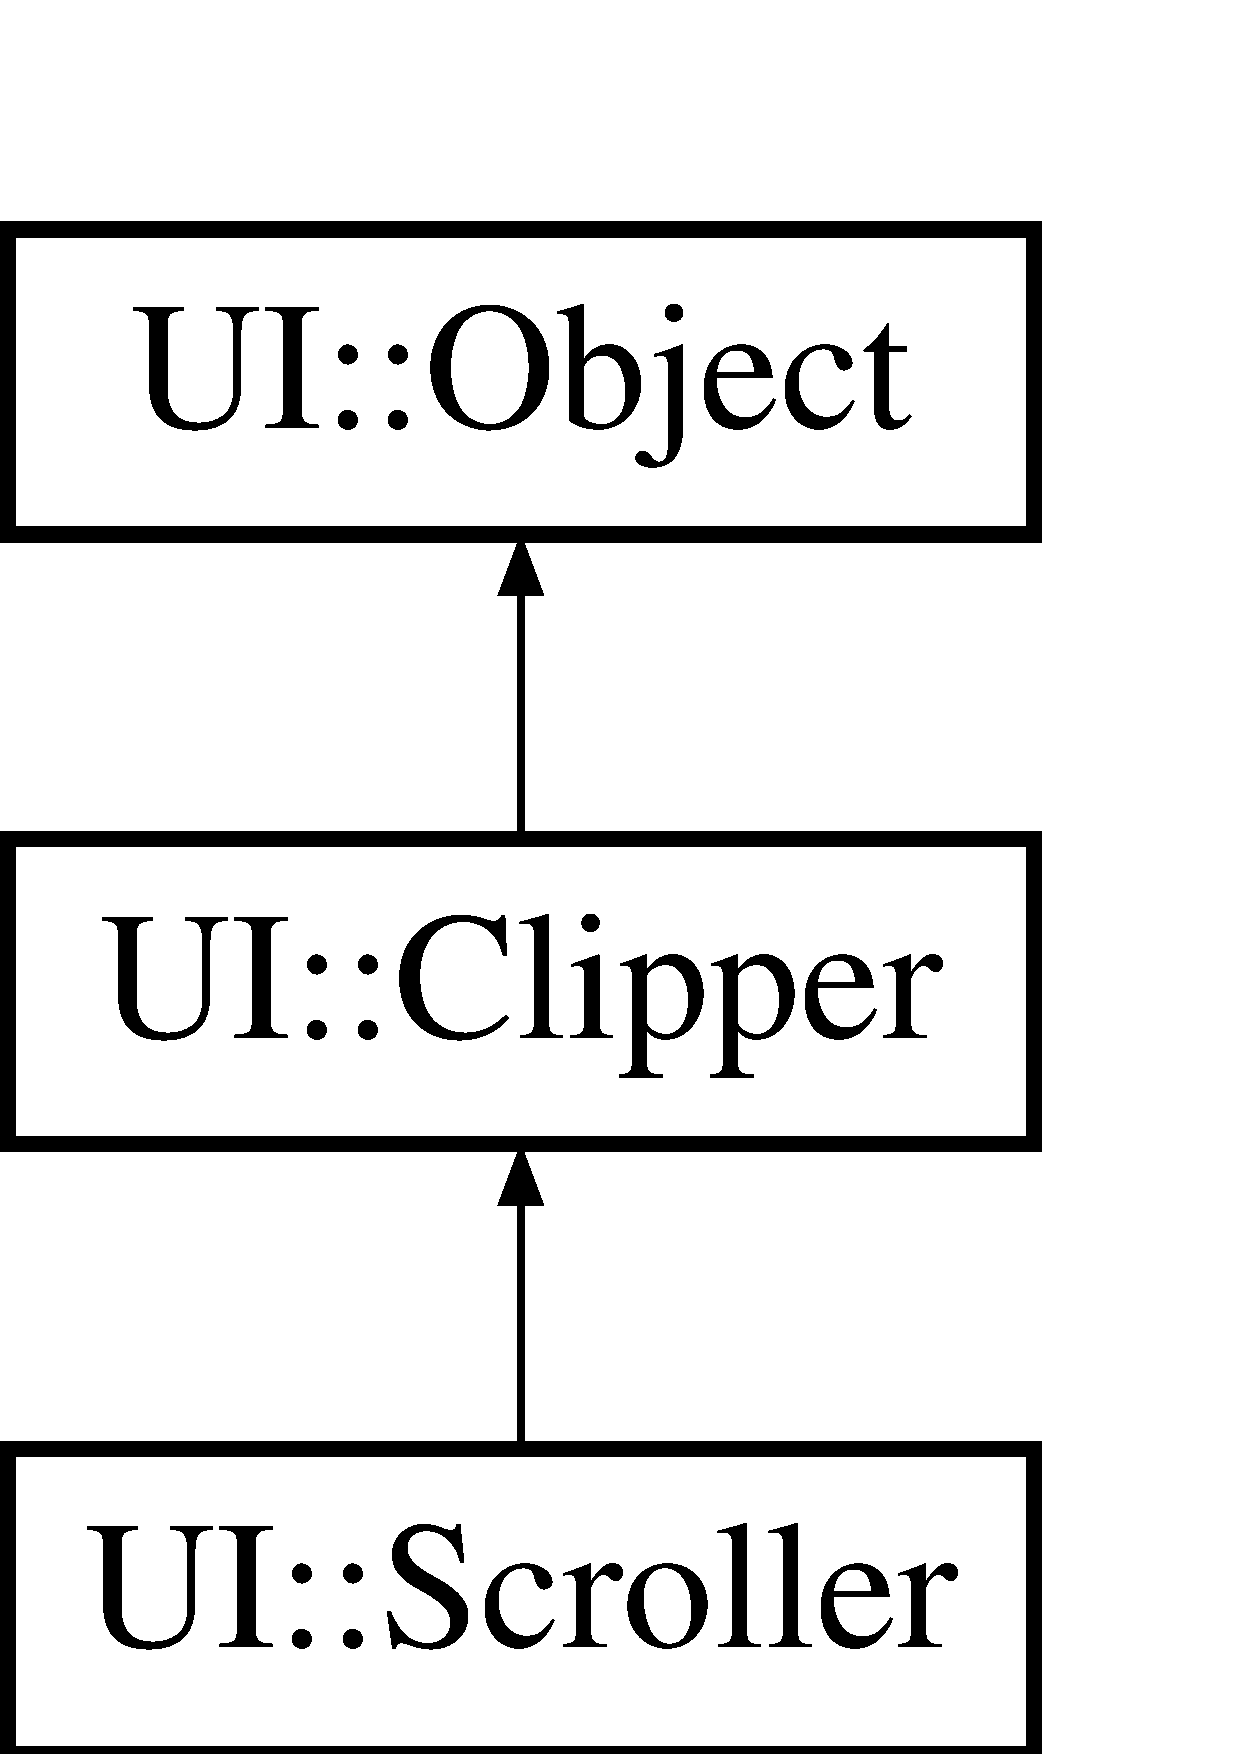
\includegraphics[height=3.000000cm]{struct_u_i_1_1_clipper}
\end{center}
\end{figure}
\subsection*{Public Member Functions}
\begin{DoxyCompactItemize}
\item 
\mbox{\Hypertarget{struct_u_i_1_1_clipper_a01aa2c0e342b6ee3475d6399d1ced702}\label{struct_u_i_1_1_clipper_a01aa2c0e342b6ee3475d6399d1ced702}} 
void {\bfseries setup} (float clipw\+\_\+=0, float cliph\+\_\+=0)
\item 
\mbox{\Hypertarget{struct_u_i_1_1_clipper_ab5dfb3bd4658b90aa5412c987f3b94d2}\label{struct_u_i_1_1_clipper_ab5dfb3bd4658b90aa5412c987f3b94d2}} 
const char $\ast$ {\bfseries gettype} () const
\item 
\mbox{\Hypertarget{struct_u_i_1_1_clipper_ab84172239e9111d89a49ee6d18d8e82e}\label{struct_u_i_1_1_clipper_ab84172239e9111d89a49ee6d18d8e82e}} 
void {\bfseries layout} ()
\item 
\mbox{\Hypertarget{struct_u_i_1_1_clipper_ad39ee9c566a6efa93e03d23eaaef5be3}\label{struct_u_i_1_1_clipper_ad39ee9c566a6efa93e03d23eaaef5be3}} 
void {\bfseries adjustchildren} ()
\item 
\mbox{\Hypertarget{struct_u_i_1_1_clipper_ac555c1baecc5c6adba4ab0ae5044eb27}\label{struct_u_i_1_1_clipper_ac555c1baecc5c6adba4ab0ae5044eb27}} 
void {\bfseries draw} (float sx, float sy)
\end{DoxyCompactItemize}
\subsection*{Static Public Member Functions}
\begin{DoxyCompactItemize}
\item 
\mbox{\Hypertarget{struct_u_i_1_1_clipper_a486295deee4091b1c6820f33f9f96411}\label{struct_u_i_1_1_clipper_a486295deee4091b1c6820f33f9f96411}} 
static const char $\ast$ {\bfseries typestr} ()
\end{DoxyCompactItemize}
\subsection*{Public Attributes}
\begin{DoxyCompactItemize}
\item 
\mbox{\Hypertarget{struct_u_i_1_1_clipper_a2791a1ba5235ba0704fd145f0e22b287}\label{struct_u_i_1_1_clipper_a2791a1ba5235ba0704fd145f0e22b287}} 
float {\bfseries clipw}
\item 
\mbox{\Hypertarget{struct_u_i_1_1_clipper_a33816e87961c0d91cae4fa26b134181e}\label{struct_u_i_1_1_clipper_a33816e87961c0d91cae4fa26b134181e}} 
float {\bfseries cliph}
\item 
\mbox{\Hypertarget{struct_u_i_1_1_clipper_aade952bb3b84f4017e625308d4b41d5e}\label{struct_u_i_1_1_clipper_aade952bb3b84f4017e625308d4b41d5e}} 
float {\bfseries virtw}
\item 
\mbox{\Hypertarget{struct_u_i_1_1_clipper_ac303b85908aac7609cc66d71d480d4a3}\label{struct_u_i_1_1_clipper_ac303b85908aac7609cc66d71d480d4a3}} 
float {\bfseries virth}
\end{DoxyCompactItemize}


The documentation for this struct was generated from the following file\+:\begin{DoxyCompactItemize}
\item 
H\+:/\+Rival\+Engine/\+Rival\+\_\+\+Game\+\_\+\+Engine\+\_\+\+G\+I\+T/\+Rival3dengine/source/engine/ui.\+cpp\end{DoxyCompactItemize}

\hypertarget{structclipplanes}{}\section{clipplanes Struct Reference}
\label{structclipplanes}\index{clipplanes@{clipplanes}}
\subsection*{Public Attributes}
\begin{DoxyCompactItemize}
\item 
\mbox{\Hypertarget{structclipplanes_a5da4fb7e93fcaa3b0be7c30e366a392f}\label{structclipplanes_a5da4fb7e93fcaa3b0be7c30e366a392f}} 
\hyperlink{structvec}{vec} {\bfseries o}
\item 
\mbox{\Hypertarget{structclipplanes_ae24b29f89e8518b64364ed7b8c85e185}\label{structclipplanes_ae24b29f89e8518b64364ed7b8c85e185}} 
\hyperlink{structvec}{vec} {\bfseries r}
\item 
\mbox{\Hypertarget{structclipplanes_a1d90cda4b387ea99e1530e009dd55b4c}\label{structclipplanes_a1d90cda4b387ea99e1530e009dd55b4c}} 
\hyperlink{structvec}{vec} {\bfseries v} \mbox{[}8\mbox{]}
\item 
\mbox{\Hypertarget{structclipplanes_a11c407435f23114b2d642a6eac15a8cf}\label{structclipplanes_a11c407435f23114b2d642a6eac15a8cf}} 
\hyperlink{structplane}{plane} {\bfseries p} \mbox{[}12\mbox{]}
\item 
\mbox{\Hypertarget{structclipplanes_a15f94cd17e5577aff13fa3106935ac20}\label{structclipplanes_a15f94cd17e5577aff13fa3106935ac20}} 
uchar {\bfseries side} \mbox{[}12\mbox{]}
\item 
\mbox{\Hypertarget{structclipplanes_a9aa5a175a030ed67c72544d609495880}\label{structclipplanes_a9aa5a175a030ed67c72544d609495880}} 
uchar {\bfseries size}
\item 
\mbox{\Hypertarget{structclipplanes_a3527cda11e5186a6562a44881ff44657}\label{structclipplanes_a3527cda11e5186a6562a44881ff44657}} 
uchar {\bfseries visible}
\item 
\mbox{\Hypertarget{structclipplanes_a9fa9954f5bf6ccdf8b26c5fff5231240}\label{structclipplanes_a9fa9954f5bf6ccdf8b26c5fff5231240}} 
const \hyperlink{structcube}{cube} $\ast$ {\bfseries owner}
\item 
\mbox{\Hypertarget{structclipplanes_af37212c0295578fefef0b274a9d4e22e}\label{structclipplanes_af37212c0295578fefef0b274a9d4e22e}} 
int {\bfseries version}
\end{DoxyCompactItemize}


The documentation for this struct was generated from the following file\+:\begin{DoxyCompactItemize}
\item 
H\+:/\+Rival\+Engine/\+Rival\+\_\+\+Game\+\_\+\+Engine\+\_\+\+G\+I\+T/\+Rival3dengine/source/engine/octa.\+h\end{DoxyCompactItemize}

\hypertarget{struct_u_i_1_1_color}{}\section{UI\+:\+:Color Struct Reference}
\label{struct_u_i_1_1_color}\index{U\+I\+::\+Color@{U\+I\+::\+Color}}
\subsection*{Public Member Functions}
\begin{DoxyCompactItemize}
\item 
\mbox{\Hypertarget{struct_u_i_1_1_color_ab39cad2acfedd778dcbb6a05440c6216}\label{struct_u_i_1_1_color_ab39cad2acfedd778dcbb6a05440c6216}} 
{\bfseries Color} (uint c)
\item 
\mbox{\Hypertarget{struct_u_i_1_1_color_a105f73289a5aa69aa921d31551ed3d2e}\label{struct_u_i_1_1_color_a105f73289a5aa69aa921d31551ed3d2e}} 
{\bfseries Color} (uint c, uchar a)
\item 
\mbox{\Hypertarget{struct_u_i_1_1_color_a3ddf38ab18328bdc11a018b1f4b9fbd2}\label{struct_u_i_1_1_color_a3ddf38ab18328bdc11a018b1f4b9fbd2}} 
{\bfseries Color} (uchar r, uchar g, uchar b, uchar a=255)
\item 
\mbox{\Hypertarget{struct_u_i_1_1_color_aacfcfb9d557646c4a0d0214df3857e0c}\label{struct_u_i_1_1_color_aacfcfb9d557646c4a0d0214df3857e0c}} 
void {\bfseries init} ()
\item 
\mbox{\Hypertarget{struct_u_i_1_1_color_a69fa265829fe080c159d72da2829c7c3}\label{struct_u_i_1_1_color_a69fa265829fe080c159d72da2829c7c3}} 
void {\bfseries attrib} ()
\end{DoxyCompactItemize}
\subsection*{Static Public Member Functions}
\begin{DoxyCompactItemize}
\item 
\mbox{\Hypertarget{struct_u_i_1_1_color_af2108f6ccfb6a4e264bab2930f300963}\label{struct_u_i_1_1_color_af2108f6ccfb6a4e264bab2930f300963}} 
static void {\bfseries def} ()
\end{DoxyCompactItemize}
\subsection*{Public Attributes}
\begin{DoxyCompactItemize}
\item 
\mbox{\Hypertarget{struct_u_i_1_1_color_a6a140223690d8f675e9ccce0b106fa58}\label{struct_u_i_1_1_color_a6a140223690d8f675e9ccce0b106fa58}} 
uchar {\bfseries r}
\item 
\mbox{\Hypertarget{struct_u_i_1_1_color_a4f80dcb2f1ca6e4b26159f2f043db255}\label{struct_u_i_1_1_color_a4f80dcb2f1ca6e4b26159f2f043db255}} 
uchar {\bfseries g}
\item 
\mbox{\Hypertarget{struct_u_i_1_1_color_a75c73d05dee66b6ff2ac287813d21e96}\label{struct_u_i_1_1_color_a75c73d05dee66b6ff2ac287813d21e96}} 
uchar {\bfseries b}
\item 
\mbox{\Hypertarget{struct_u_i_1_1_color_a884cb8b7293661142208d9f3de9ac2a3}\label{struct_u_i_1_1_color_a884cb8b7293661142208d9f3de9ac2a3}} 
uchar {\bfseries a}
\end{DoxyCompactItemize}


The documentation for this struct was generated from the following file\+:\begin{DoxyCompactItemize}
\item 
H\+:/\+Rival\+Engine/\+Rival\+\_\+\+Game\+\_\+\+Engine\+\_\+\+G\+I\+T/\+Rival3dengine/source/engine/ui.\+cpp\end{DoxyCompactItemize}

\hypertarget{struct_u_i_1_1_console}{}\section{UI\+:\+:Console Struct Reference}
\label{struct_u_i_1_1_console}\index{U\+I\+::\+Console@{U\+I\+::\+Console}}
Inheritance diagram for UI\+:\+:Console\+:\begin{figure}[H]
\begin{center}
\leavevmode
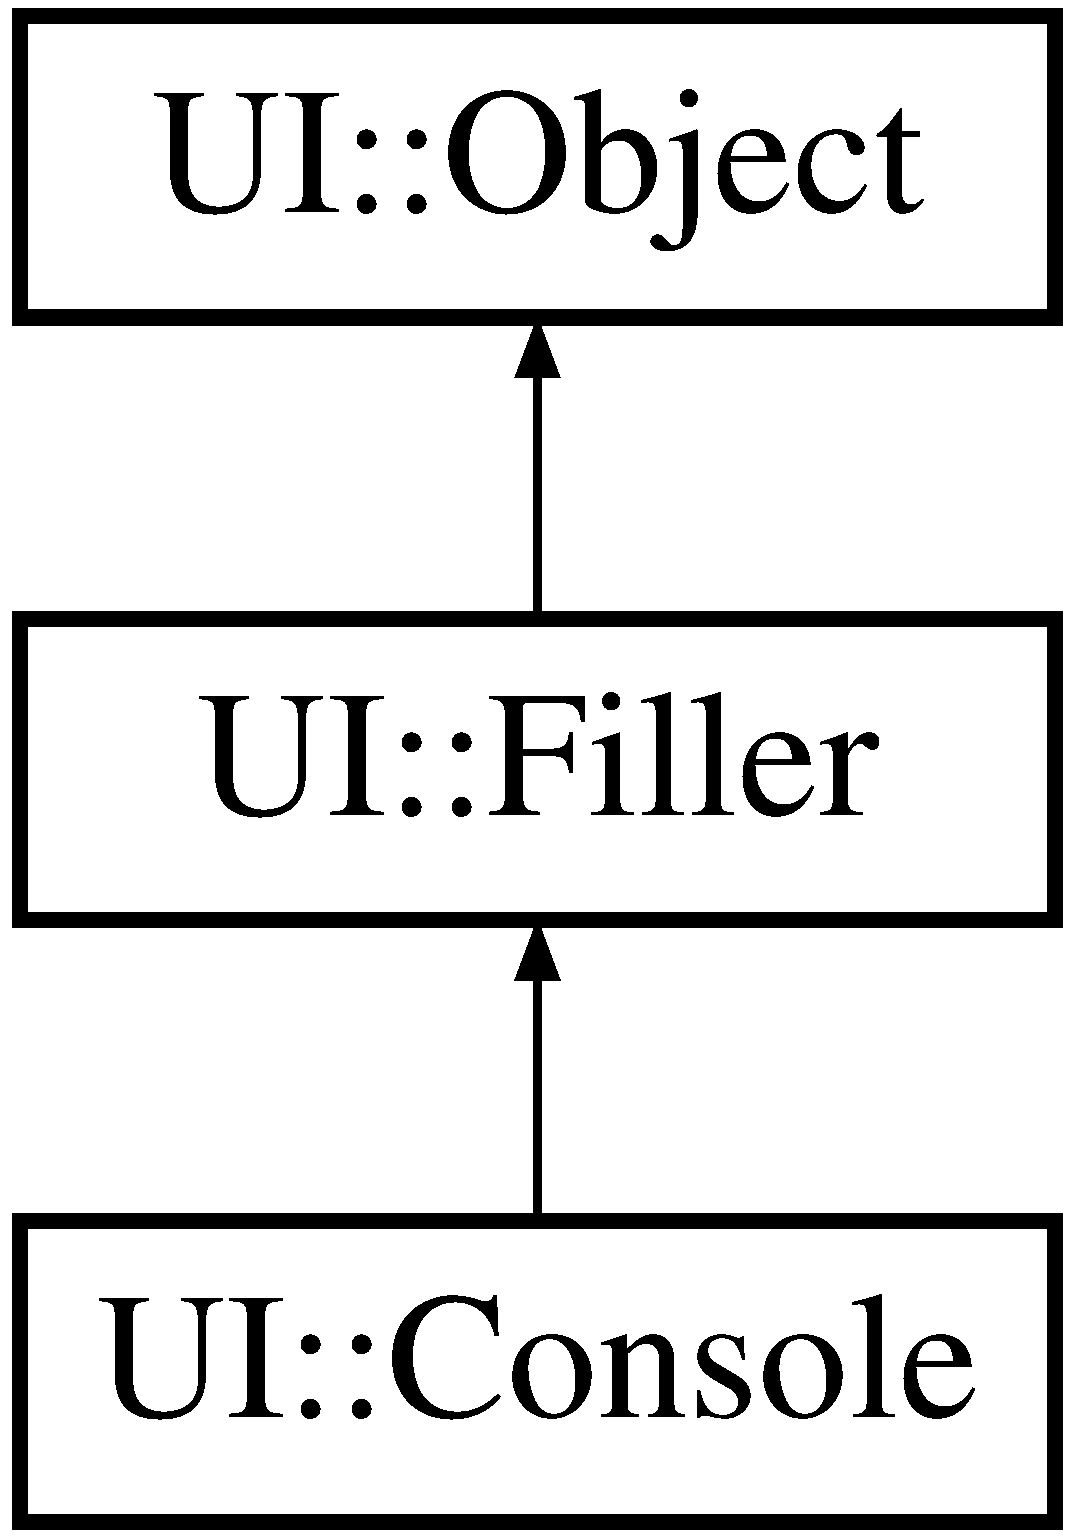
\includegraphics[height=3.000000cm]{struct_u_i_1_1_console}
\end{center}
\end{figure}
\subsection*{Public Member Functions}
\begin{DoxyCompactItemize}
\item 
\mbox{\Hypertarget{struct_u_i_1_1_console_a6a0e13ebd65794e88fe84ae63133dd8f}\label{struct_u_i_1_1_console_a6a0e13ebd65794e88fe84ae63133dd8f}} 
void {\bfseries setup} (float minw\+\_\+=0, float minh\+\_\+=0)
\item 
\mbox{\Hypertarget{struct_u_i_1_1_console_a2278d17e86b8c287bafa6417cbde8296}\label{struct_u_i_1_1_console_a2278d17e86b8c287bafa6417cbde8296}} 
const char $\ast$ {\bfseries gettype} () const
\item 
\mbox{\Hypertarget{struct_u_i_1_1_console_abe603f224bd7e4677519da82c592cc89}\label{struct_u_i_1_1_console_abe603f224bd7e4677519da82c592cc89}} 
float {\bfseries drawscale} () const
\item 
\mbox{\Hypertarget{struct_u_i_1_1_console_a55e6d17b17da10a211067d1ec0db89b1}\label{struct_u_i_1_1_console_a55e6d17b17da10a211067d1ec0db89b1}} 
void {\bfseries draw} (float sx, float sy)
\end{DoxyCompactItemize}
\subsection*{Static Public Member Functions}
\begin{DoxyCompactItemize}
\item 
\mbox{\Hypertarget{struct_u_i_1_1_console_a1738f5f02a921cab287ca603be4d6598}\label{struct_u_i_1_1_console_a1738f5f02a921cab287ca603be4d6598}} 
static const char $\ast$ {\bfseries typestr} ()
\end{DoxyCompactItemize}
\subsection*{Additional Inherited Members}


The documentation for this struct was generated from the following file\+:\begin{DoxyCompactItemize}
\item 
H\+:/\+Rival\+Engine/\+Rival\+\_\+\+Game\+\_\+\+Engine\+\_\+\+G\+I\+T/\+Rival3dengine/source/engine/ui.\+cpp\end{DoxyCompactItemize}

\hypertarget{structserver_1_1crcinfo}{}\section{server\+:\+:crcinfo Struct Reference}
\label{structserver_1_1crcinfo}\index{server\+::crcinfo@{server\+::crcinfo}}
\subsection*{Public Member Functions}
\begin{DoxyCompactItemize}
\item 
\mbox{\Hypertarget{structserver_1_1crcinfo_acfc8df852fbd83f97b29d40ac0c4748c}\label{structserver_1_1crcinfo_acfc8df852fbd83f97b29d40ac0c4748c}} 
{\bfseries crcinfo} (int crc, int matches)
\end{DoxyCompactItemize}
\subsection*{Static Public Member Functions}
\begin{DoxyCompactItemize}
\item 
\mbox{\Hypertarget{structserver_1_1crcinfo_ad09fe4a3fae8e872f603636b831d4dca}\label{structserver_1_1crcinfo_ad09fe4a3fae8e872f603636b831d4dca}} 
static bool {\bfseries compare} (const \hyperlink{structserver_1_1crcinfo}{crcinfo} \&x, const \hyperlink{structserver_1_1crcinfo}{crcinfo} \&y)
\end{DoxyCompactItemize}
\subsection*{Public Attributes}
\begin{DoxyCompactItemize}
\item 
\mbox{\Hypertarget{structserver_1_1crcinfo_ae0722e68e926d77d761430071c2ce1f8}\label{structserver_1_1crcinfo_ae0722e68e926d77d761430071c2ce1f8}} 
int {\bfseries crc}
\item 
\mbox{\Hypertarget{structserver_1_1crcinfo_afc558b8cc6c75c71a30498fd3bf92b45}\label{structserver_1_1crcinfo_afc558b8cc6c75c71a30498fd3bf92b45}} 
int {\bfseries matches}
\end{DoxyCompactItemize}


The documentation for this struct was generated from the following file\+:\begin{DoxyCompactItemize}
\item 
H\+:/\+Rival\+Engine/\+Rival\+\_\+\+Game\+\_\+\+Engine\+\_\+\+G\+I\+T/\+Rival3dengine/source/game/server.\+cpp\end{DoxyCompactItemize}

\hypertarget{struct_u_i_1_1_cropped_image}{}\section{UI\+:\+:Cropped\+Image Struct Reference}
\label{struct_u_i_1_1_cropped_image}\index{U\+I\+::\+Cropped\+Image@{U\+I\+::\+Cropped\+Image}}
Inheritance diagram for UI\+:\+:Cropped\+Image\+:\begin{figure}[H]
\begin{center}
\leavevmode
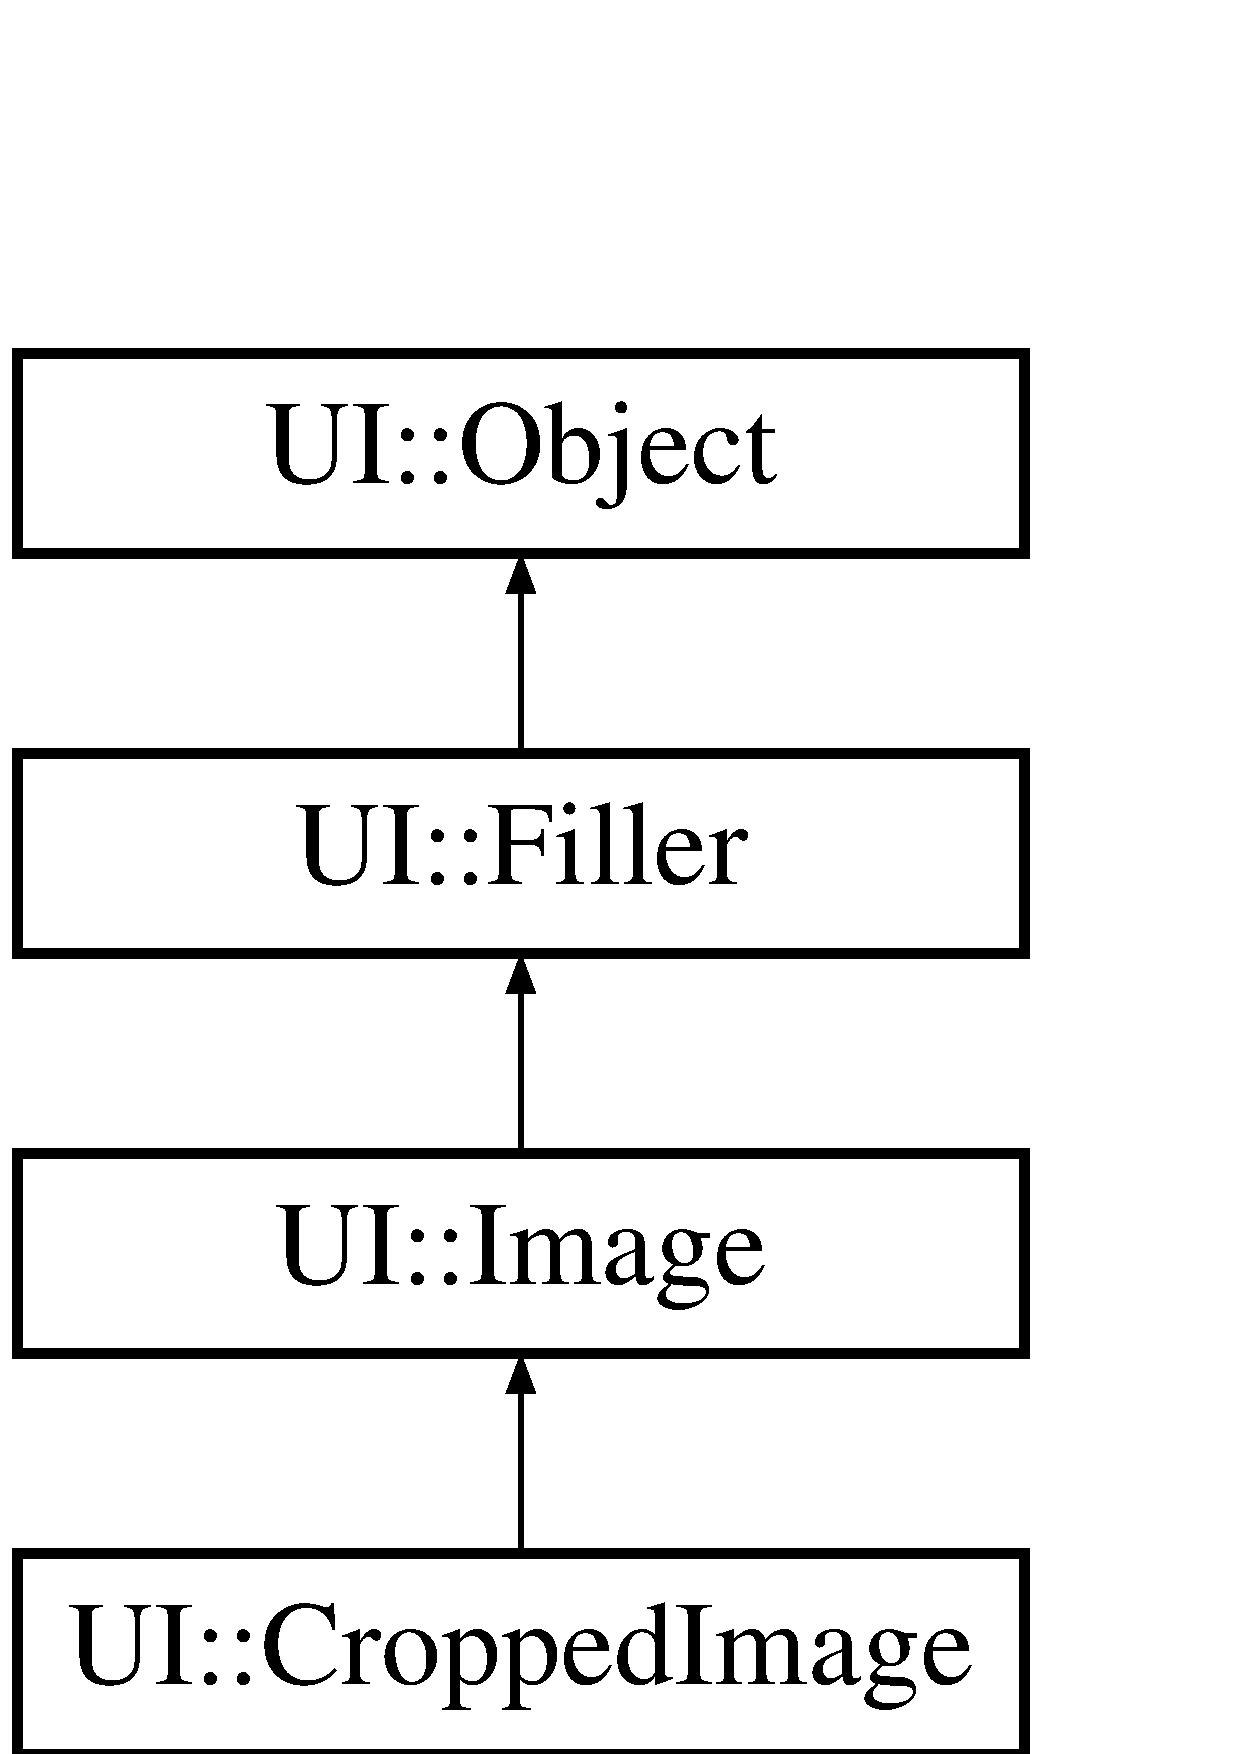
\includegraphics[height=4.000000cm]{struct_u_i_1_1_cropped_image}
\end{center}
\end{figure}
\subsection*{Public Member Functions}
\begin{DoxyCompactItemize}
\item 
\mbox{\Hypertarget{struct_u_i_1_1_cropped_image_a61b066fde1da2cc5e8b07c649062bb50}\label{struct_u_i_1_1_cropped_image_a61b066fde1da2cc5e8b07c649062bb50}} 
void {\bfseries setup} (\hyperlink{struct_texture}{Texture} $\ast$tex\+\_\+, float minw\+\_\+=0, float minh\+\_\+=0, float cropx\+\_\+=0, float cropy\+\_\+=0, float cropw\+\_\+=1, float croph\+\_\+=1)
\item 
\mbox{\Hypertarget{struct_u_i_1_1_cropped_image_afae078dd3aae2f02aefd0d1d0104d535}\label{struct_u_i_1_1_cropped_image_afae078dd3aae2f02aefd0d1d0104d535}} 
const char $\ast$ {\bfseries gettype} () const
\item 
\mbox{\Hypertarget{struct_u_i_1_1_cropped_image_a3b5fce6f7cd8b1cbe81097f969b508cb}\label{struct_u_i_1_1_cropped_image_a3b5fce6f7cd8b1cbe81097f969b508cb}} 
bool {\bfseries target} (float cx, float cy)
\item 
\mbox{\Hypertarget{struct_u_i_1_1_cropped_image_a45f3158330fe19f463b0d82815c8604e}\label{struct_u_i_1_1_cropped_image_a45f3158330fe19f463b0d82815c8604e}} 
void {\bfseries draw} (float sx, float sy)
\end{DoxyCompactItemize}
\subsection*{Static Public Member Functions}
\begin{DoxyCompactItemize}
\item 
\mbox{\Hypertarget{struct_u_i_1_1_cropped_image_a3512429c7606eaa52f9bf37e86477468}\label{struct_u_i_1_1_cropped_image_a3512429c7606eaa52f9bf37e86477468}} 
static const char $\ast$ {\bfseries typestr} ()
\end{DoxyCompactItemize}
\subsection*{Public Attributes}
\begin{DoxyCompactItemize}
\item 
\mbox{\Hypertarget{struct_u_i_1_1_cropped_image_af95202739e42261310d00b2b90486cfa}\label{struct_u_i_1_1_cropped_image_af95202739e42261310d00b2b90486cfa}} 
float {\bfseries cropx}
\item 
\mbox{\Hypertarget{struct_u_i_1_1_cropped_image_a5f21c6523787dfe187e779eb6ec07184}\label{struct_u_i_1_1_cropped_image_a5f21c6523787dfe187e779eb6ec07184}} 
float {\bfseries cropy}
\item 
\mbox{\Hypertarget{struct_u_i_1_1_cropped_image_aa917c3b6e41a5014eec3c246537ccbe5}\label{struct_u_i_1_1_cropped_image_aa917c3b6e41a5014eec3c246537ccbe5}} 
float {\bfseries cropw}
\item 
\mbox{\Hypertarget{struct_u_i_1_1_cropped_image_aae518ee79e4e6828d12fa7fa9617c799}\label{struct_u_i_1_1_cropped_image_aae518ee79e4e6828d12fa7fa9617c799}} 
float {\bfseries croph}
\end{DoxyCompactItemize}
\subsection*{Additional Inherited Members}


The documentation for this struct was generated from the following file\+:\begin{DoxyCompactItemize}
\item 
H\+:/\+Rival\+Engine/\+Rival\+\_\+\+Game\+\_\+\+Engine\+\_\+\+G\+I\+T/\+Rival3dengine/source/engine/ui.\+cpp\end{DoxyCompactItemize}

\hypertarget{class_c_script_array}{}\section{C\+Script\+Array Class Reference}
\label{class_c_script_array}\index{C\+Script\+Array@{C\+Script\+Array}}
\subsection*{Public Member Functions}
\begin{DoxyCompactItemize}
\item 
\mbox{\Hypertarget{class_c_script_array_a23d70e828e8bee3c9dce09e602836086}\label{class_c_script_array_a23d70e828e8bee3c9dce09e602836086}} 
void {\bfseries Add\+Ref} () const
\item 
\mbox{\Hypertarget{class_c_script_array_ade6e4b39fda93c29304563f5647a5677}\label{class_c_script_array_ade6e4b39fda93c29304563f5647a5677}} 
void {\bfseries Release} () const
\item 
\mbox{\Hypertarget{class_c_script_array_acc2b8af2504d9b4effef5012bd6f3940}\label{class_c_script_array_acc2b8af2504d9b4effef5012bd6f3940}} 
\hyperlink{classas_i_type_info}{as\+I\+Type\+Info} $\ast$ {\bfseries Get\+Array\+Object\+Type} () const
\item 
\mbox{\Hypertarget{class_c_script_array_a39c5bdd243adf6b2a3236d10cb0dc00c}\label{class_c_script_array_a39c5bdd243adf6b2a3236d10cb0dc00c}} 
int {\bfseries Get\+Array\+Type\+Id} () const
\item 
\mbox{\Hypertarget{class_c_script_array_aea5620585756a886e658c651bcae4b7b}\label{class_c_script_array_aea5620585756a886e658c651bcae4b7b}} 
int {\bfseries Get\+Element\+Type\+Id} () const
\item 
\mbox{\Hypertarget{class_c_script_array_a9ee3347ed075a05718e3946032d4c117}\label{class_c_script_array_a9ee3347ed075a05718e3946032d4c117}} 
as\+U\+I\+NT {\bfseries Get\+Size} () const
\item 
\mbox{\Hypertarget{class_c_script_array_a2577f61bf0fa86ac4602d0b909098857}\label{class_c_script_array_a2577f61bf0fa86ac4602d0b909098857}} 
bool {\bfseries Is\+Empty} () const
\item 
\mbox{\Hypertarget{class_c_script_array_ae0b270ff8220f9678a5a7d572abf495d}\label{class_c_script_array_ae0b270ff8220f9678a5a7d572abf495d}} 
void {\bfseries Reserve} (as\+U\+I\+NT max\+Elements)
\item 
\mbox{\Hypertarget{class_c_script_array_a54fe13adf1cdded2aec4ac0b5924891f}\label{class_c_script_array_a54fe13adf1cdded2aec4ac0b5924891f}} 
void {\bfseries Resize} (as\+U\+I\+NT num\+Elements)
\item 
\mbox{\Hypertarget{class_c_script_array_ac179b031c789763b6d7cecb8c07157f5}\label{class_c_script_array_ac179b031c789763b6d7cecb8c07157f5}} 
void $\ast$ {\bfseries At} (as\+U\+I\+NT index)
\item 
\mbox{\Hypertarget{class_c_script_array_ab0a2decafb780ad7bbbc9c69a308b3c9}\label{class_c_script_array_ab0a2decafb780ad7bbbc9c69a308b3c9}} 
const void $\ast$ {\bfseries At} (as\+U\+I\+NT index) const
\item 
\mbox{\Hypertarget{class_c_script_array_ad84bc1e1fb44fe34fffa5d46c389a09f}\label{class_c_script_array_ad84bc1e1fb44fe34fffa5d46c389a09f}} 
void {\bfseries Set\+Value} (as\+U\+I\+NT index, void $\ast$value)
\item 
\mbox{\Hypertarget{class_c_script_array_a9b4e1b2726012e83b6426bd1f2863075}\label{class_c_script_array_a9b4e1b2726012e83b6426bd1f2863075}} 
\hyperlink{class_c_script_array}{C\+Script\+Array} \& {\bfseries operator=} (const \hyperlink{class_c_script_array}{C\+Script\+Array} \&)
\item 
\mbox{\Hypertarget{class_c_script_array_a3b4ee8c5da2348f7f22558b73763e2e0}\label{class_c_script_array_a3b4ee8c5da2348f7f22558b73763e2e0}} 
bool {\bfseries operator==} (const \hyperlink{class_c_script_array}{C\+Script\+Array} \&) const
\item 
\mbox{\Hypertarget{class_c_script_array_a5783becfa2a47a1e0216475b96698cd5}\label{class_c_script_array_a5783becfa2a47a1e0216475b96698cd5}} 
void {\bfseries Insert\+At} (as\+U\+I\+NT index, void $\ast$value)
\item 
\mbox{\Hypertarget{class_c_script_array_a9171c3d542fdab793218947fa7b33a6a}\label{class_c_script_array_a9171c3d542fdab793218947fa7b33a6a}} 
void {\bfseries Insert\+At} (as\+U\+I\+NT index, const \hyperlink{class_c_script_array}{C\+Script\+Array} \&arr)
\item 
\mbox{\Hypertarget{class_c_script_array_ab885ff32eed1bb81d599fbf46e30915f}\label{class_c_script_array_ab885ff32eed1bb81d599fbf46e30915f}} 
void {\bfseries Insert\+Last} (void $\ast$value)
\item 
\mbox{\Hypertarget{class_c_script_array_a569bab2097259d4373c080affdf958f3}\label{class_c_script_array_a569bab2097259d4373c080affdf958f3}} 
void {\bfseries Remove\+At} (as\+U\+I\+NT index)
\item 
\mbox{\Hypertarget{class_c_script_array_a067270b5841aeb55e42e53e6e26bcfb1}\label{class_c_script_array_a067270b5841aeb55e42e53e6e26bcfb1}} 
void {\bfseries Remove\+Last} ()
\item 
\mbox{\Hypertarget{class_c_script_array_aefdefe99e23064e7661a1e15db951d82}\label{class_c_script_array_aefdefe99e23064e7661a1e15db951d82}} 
void {\bfseries Remove\+Range} (as\+U\+I\+NT start, as\+U\+I\+NT count)
\item 
\mbox{\Hypertarget{class_c_script_array_aebf917c3e702d90901eef9f89ffa0e0c}\label{class_c_script_array_aebf917c3e702d90901eef9f89ffa0e0c}} 
void {\bfseries Sort\+Asc} ()
\item 
\mbox{\Hypertarget{class_c_script_array_a9d0cb19caa89bdb834af07b1f1e23372}\label{class_c_script_array_a9d0cb19caa89bdb834af07b1f1e23372}} 
void {\bfseries Sort\+Desc} ()
\item 
\mbox{\Hypertarget{class_c_script_array_a321f75202e3b99cf718b8866e4a076e4}\label{class_c_script_array_a321f75202e3b99cf718b8866e4a076e4}} 
void {\bfseries Sort\+Asc} (as\+U\+I\+NT start\+At, as\+U\+I\+NT count)
\item 
\mbox{\Hypertarget{class_c_script_array_a950a4cfa57f2bd198ab48c32d2e09abd}\label{class_c_script_array_a950a4cfa57f2bd198ab48c32d2e09abd}} 
void {\bfseries Sort\+Desc} (as\+U\+I\+NT start\+At, as\+U\+I\+NT count)
\item 
\mbox{\Hypertarget{class_c_script_array_a0a2c287920ed349cb94c7fbea933a555}\label{class_c_script_array_a0a2c287920ed349cb94c7fbea933a555}} 
void {\bfseries Sort} (as\+U\+I\+NT start\+At, as\+U\+I\+NT count, bool asc)
\item 
\mbox{\Hypertarget{class_c_script_array_aa41319c81b80f50e2be977db7d2cdb54}\label{class_c_script_array_aa41319c81b80f50e2be977db7d2cdb54}} 
void {\bfseries Reverse} ()
\item 
\mbox{\Hypertarget{class_c_script_array_aa52ed5b77c1d312b4dfbb083b77c277c}\label{class_c_script_array_aa52ed5b77c1d312b4dfbb083b77c277c}} 
int {\bfseries Find} (void $\ast$value) const
\item 
\mbox{\Hypertarget{class_c_script_array_abfb65e53fcf6cfb1f86a76a04de0610b}\label{class_c_script_array_abfb65e53fcf6cfb1f86a76a04de0610b}} 
int {\bfseries Find} (as\+U\+I\+NT start\+At, void $\ast$value) const
\item 
\mbox{\Hypertarget{class_c_script_array_adfc875eb0bb5ff6e434c73ec88663468}\label{class_c_script_array_adfc875eb0bb5ff6e434c73ec88663468}} 
int {\bfseries Find\+By\+Ref} (void $\ast$ref) const
\item 
\mbox{\Hypertarget{class_c_script_array_ac6db58124311bc10d31a406c1b704034}\label{class_c_script_array_ac6db58124311bc10d31a406c1b704034}} 
int {\bfseries Find\+By\+Ref} (as\+U\+I\+NT start\+At, void $\ast$ref) const
\item 
\mbox{\Hypertarget{class_c_script_array_a098920427fa8395f8826ac1146e608dd}\label{class_c_script_array_a098920427fa8395f8826ac1146e608dd}} 
void $\ast$ {\bfseries Get\+Buffer} ()
\item 
\mbox{\Hypertarget{class_c_script_array_a0930872210110d97174b9e731dcd9223}\label{class_c_script_array_a0930872210110d97174b9e731dcd9223}} 
int {\bfseries Get\+Ref\+Count} ()
\item 
\mbox{\Hypertarget{class_c_script_array_a7a5bb10b3f4ed45a19e3e4af92cee03e}\label{class_c_script_array_a7a5bb10b3f4ed45a19e3e4af92cee03e}} 
void {\bfseries Set\+Flag} ()
\item 
\mbox{\Hypertarget{class_c_script_array_aca4e57f9d07233882048f83665a22317}\label{class_c_script_array_aca4e57f9d07233882048f83665a22317}} 
bool {\bfseries Get\+Flag} ()
\item 
\mbox{\Hypertarget{class_c_script_array_ac2fbae4819e642ff82c8b31439e17cb2}\label{class_c_script_array_ac2fbae4819e642ff82c8b31439e17cb2}} 
void {\bfseries Enum\+References} (\hyperlink{classas_i_script_engine}{as\+I\+Script\+Engine} $\ast$engine)
\item 
\mbox{\Hypertarget{class_c_script_array_acf0576a959d4710c35a7073046748de7}\label{class_c_script_array_acf0576a959d4710c35a7073046748de7}} 
void {\bfseries Release\+All\+Handles} (\hyperlink{classas_i_script_engine}{as\+I\+Script\+Engine} $\ast$engine)
\end{DoxyCompactItemize}
\subsection*{Static Public Member Functions}
\begin{DoxyCompactItemize}
\item 
\mbox{\Hypertarget{class_c_script_array_a04daa9f9f1234fc48adacc5369df736d}\label{class_c_script_array_a04daa9f9f1234fc48adacc5369df736d}} 
static void {\bfseries Set\+Memory\+Functions} (as\+A\+L\+L\+O\+C\+F\+U\+N\+C\+\_\+t alloc\+Func, as\+F\+R\+E\+E\+F\+U\+N\+C\+\_\+t free\+Func)
\item 
\mbox{\Hypertarget{class_c_script_array_a64ed669277c5069790175d49e29362c2}\label{class_c_script_array_a64ed669277c5069790175d49e29362c2}} 
static \hyperlink{class_c_script_array}{C\+Script\+Array} $\ast$ {\bfseries Create} (\hyperlink{classas_i_type_info}{as\+I\+Type\+Info} $\ast$ot)
\item 
\mbox{\Hypertarget{class_c_script_array_a257441650a704b9483c2c5d7a554459f}\label{class_c_script_array_a257441650a704b9483c2c5d7a554459f}} 
static \hyperlink{class_c_script_array}{C\+Script\+Array} $\ast$ {\bfseries Create} (\hyperlink{classas_i_type_info}{as\+I\+Type\+Info} $\ast$ot, as\+U\+I\+NT length)
\item 
\mbox{\Hypertarget{class_c_script_array_a33d70a59a585eccc6c3630be62675960}\label{class_c_script_array_a33d70a59a585eccc6c3630be62675960}} 
static \hyperlink{class_c_script_array}{C\+Script\+Array} $\ast$ {\bfseries Create} (\hyperlink{classas_i_type_info}{as\+I\+Type\+Info} $\ast$ot, as\+U\+I\+NT length, void $\ast$default\+Value)
\item 
\mbox{\Hypertarget{class_c_script_array_a868e06f7f0b54b8f5ee8b3c68366d5af}\label{class_c_script_array_a868e06f7f0b54b8f5ee8b3c68366d5af}} 
static \hyperlink{class_c_script_array}{C\+Script\+Array} $\ast$ {\bfseries Create} (\hyperlink{classas_i_type_info}{as\+I\+Type\+Info} $\ast$ot, void $\ast$list\+Buffer)
\end{DoxyCompactItemize}
\subsection*{Protected Member Functions}
\begin{DoxyCompactItemize}
\item 
\mbox{\Hypertarget{class_c_script_array_a6f5c46cbb303342f09b45a4701db0fcc}\label{class_c_script_array_a6f5c46cbb303342f09b45a4701db0fcc}} 
{\bfseries C\+Script\+Array} (\hyperlink{classas_i_type_info}{as\+I\+Type\+Info} $\ast$ot, void $\ast$init\+Buf)
\item 
\mbox{\Hypertarget{class_c_script_array_a4f648c7b544c95f2d87efe5b8030cc02}\label{class_c_script_array_a4f648c7b544c95f2d87efe5b8030cc02}} 
{\bfseries C\+Script\+Array} (as\+U\+I\+NT length, \hyperlink{classas_i_type_info}{as\+I\+Type\+Info} $\ast$ot)
\item 
\mbox{\Hypertarget{class_c_script_array_ad5112daf3be11e9d9d0a2341dc4d1cd2}\label{class_c_script_array_ad5112daf3be11e9d9d0a2341dc4d1cd2}} 
{\bfseries C\+Script\+Array} (as\+U\+I\+NT length, void $\ast$def\+Val, \hyperlink{classas_i_type_info}{as\+I\+Type\+Info} $\ast$ot)
\item 
\mbox{\Hypertarget{class_c_script_array_a0febe0c884c02f2b1efb4d73417d2bcf}\label{class_c_script_array_a0febe0c884c02f2b1efb4d73417d2bcf}} 
{\bfseries C\+Script\+Array} (const \hyperlink{class_c_script_array}{C\+Script\+Array} \&other)
\item 
\mbox{\Hypertarget{class_c_script_array_a76531ec8ed4b809a6f18ea989c9ef79a}\label{class_c_script_array_a76531ec8ed4b809a6f18ea989c9ef79a}} 
bool {\bfseries Less} (const void $\ast$a, const void $\ast$b, bool asc, \hyperlink{classas_i_script_context}{as\+I\+Script\+Context} $\ast$ctx, \hyperlink{struct_s_array_cache}{S\+Array\+Cache} $\ast$cache)
\item 
\mbox{\Hypertarget{class_c_script_array_aa8316ebce329c3b187a883b384623e2d}\label{class_c_script_array_aa8316ebce329c3b187a883b384623e2d}} 
void $\ast$ {\bfseries Get\+Array\+Item\+Pointer} (int index)
\item 
\mbox{\Hypertarget{class_c_script_array_a96c38b510f6b5650de200636b53b0e6b}\label{class_c_script_array_a96c38b510f6b5650de200636b53b0e6b}} 
void $\ast$ {\bfseries Get\+Data\+Pointer} (void $\ast$buffer)
\item 
\mbox{\Hypertarget{class_c_script_array_abf5a7cbf943e08be36aba4a1efc5c61f}\label{class_c_script_array_abf5a7cbf943e08be36aba4a1efc5c61f}} 
void {\bfseries Copy} (void $\ast$dst, void $\ast$src)
\item 
\mbox{\Hypertarget{class_c_script_array_aad3ec13ab9a83bcec2238b0f5e0da49e}\label{class_c_script_array_aad3ec13ab9a83bcec2238b0f5e0da49e}} 
void {\bfseries Precache} ()
\item 
\mbox{\Hypertarget{class_c_script_array_a7b0f5d403c859b4b3d3af2c6eb1f468c}\label{class_c_script_array_a7b0f5d403c859b4b3d3af2c6eb1f468c}} 
bool {\bfseries Check\+Max\+Size} (as\+U\+I\+NT num\+Elements)
\item 
\mbox{\Hypertarget{class_c_script_array_ae8a62ceca782c341f7a6786c578d3353}\label{class_c_script_array_ae8a62ceca782c341f7a6786c578d3353}} 
void {\bfseries Resize} (int delta, as\+U\+I\+NT at)
\item 
\mbox{\Hypertarget{class_c_script_array_a4ed53d161ece72db045d1dee83e2957e}\label{class_c_script_array_a4ed53d161ece72db045d1dee83e2957e}} 
void {\bfseries Create\+Buffer} (\hyperlink{struct_s_array_buffer}{S\+Array\+Buffer} $\ast$$\ast$buf, as\+U\+I\+NT num\+Elements)
\item 
\mbox{\Hypertarget{class_c_script_array_a7dfbb455d13c71170d86b85ac947c2c8}\label{class_c_script_array_a7dfbb455d13c71170d86b85ac947c2c8}} 
void {\bfseries Delete\+Buffer} (\hyperlink{struct_s_array_buffer}{S\+Array\+Buffer} $\ast$buf)
\item 
\mbox{\Hypertarget{class_c_script_array_a4b9de4ef151094e8d9c3879e28cbbf73}\label{class_c_script_array_a4b9de4ef151094e8d9c3879e28cbbf73}} 
void {\bfseries Copy\+Buffer} (\hyperlink{struct_s_array_buffer}{S\+Array\+Buffer} $\ast$dst, \hyperlink{struct_s_array_buffer}{S\+Array\+Buffer} $\ast$src)
\item 
\mbox{\Hypertarget{class_c_script_array_a2d7d226b6df50e0e5b77aef8bb85e205}\label{class_c_script_array_a2d7d226b6df50e0e5b77aef8bb85e205}} 
void {\bfseries Construct} (\hyperlink{struct_s_array_buffer}{S\+Array\+Buffer} $\ast$buf, as\+U\+I\+NT start, as\+U\+I\+NT end)
\item 
\mbox{\Hypertarget{class_c_script_array_a12549b933e3a8aadb678bf282b31e94b}\label{class_c_script_array_a12549b933e3a8aadb678bf282b31e94b}} 
void {\bfseries Destruct} (\hyperlink{struct_s_array_buffer}{S\+Array\+Buffer} $\ast$buf, as\+U\+I\+NT start, as\+U\+I\+NT end)
\item 
\mbox{\Hypertarget{class_c_script_array_a36125c507bc5a1576765b763fdc76d04}\label{class_c_script_array_a36125c507bc5a1576765b763fdc76d04}} 
bool {\bfseries Equals} (const void $\ast$a, const void $\ast$b, \hyperlink{classas_i_script_context}{as\+I\+Script\+Context} $\ast$ctx, \hyperlink{struct_s_array_cache}{S\+Array\+Cache} $\ast$cache) const
\end{DoxyCompactItemize}
\subsection*{Protected Attributes}
\begin{DoxyCompactItemize}
\item 
\mbox{\Hypertarget{class_c_script_array_ac2ada6d851d5e606ecaf915805e411c6}\label{class_c_script_array_ac2ada6d851d5e606ecaf915805e411c6}} 
int {\bfseries ref\+Count}
\item 
\mbox{\Hypertarget{class_c_script_array_ad9b81bca74db2f95bb71f70b63b3eda6}\label{class_c_script_array_ad9b81bca74db2f95bb71f70b63b3eda6}} 
bool {\bfseries gc\+Flag}
\item 
\mbox{\Hypertarget{class_c_script_array_a13f504dcd4f6e6a096a8afb632ff8f90}\label{class_c_script_array_a13f504dcd4f6e6a096a8afb632ff8f90}} 
\hyperlink{classas_i_type_info}{as\+I\+Type\+Info} $\ast$ {\bfseries obj\+Type}
\item 
\mbox{\Hypertarget{class_c_script_array_a60601db371fb5f7a0b19a29078c9ec66}\label{class_c_script_array_a60601db371fb5f7a0b19a29078c9ec66}} 
\hyperlink{struct_s_array_buffer}{S\+Array\+Buffer} $\ast$ {\bfseries buffer}
\item 
\mbox{\Hypertarget{class_c_script_array_aeef72ead23390babbf2502381a469419}\label{class_c_script_array_aeef72ead23390babbf2502381a469419}} 
int {\bfseries element\+Size}
\item 
\mbox{\Hypertarget{class_c_script_array_a9d112cbe0aba514e3551e30908903215}\label{class_c_script_array_a9d112cbe0aba514e3551e30908903215}} 
int {\bfseries sub\+Type\+Id}
\end{DoxyCompactItemize}


The documentation for this class was generated from the following files\+:\begin{DoxyCompactItemize}
\item 
H\+:/\+Rival\+Engine/\+Rival\+\_\+\+Game\+\_\+\+Engine\+\_\+\+G\+I\+T/\+Rival3dengine/source/shared/scriptarray.\+h\item 
H\+:/\+Rival\+Engine/\+Rival\+\_\+\+Game\+\_\+\+Engine\+\_\+\+G\+I\+T/\+Rival3dengine/source/shared/scriptarray.\+cpp\end{DoxyCompactItemize}

\hypertarget{class_c_script_builder}{}\section{C\+Script\+Builder Class Reference}
\label{class_c_script_builder}\index{C\+Script\+Builder@{C\+Script\+Builder}}
\subsection*{Classes}
\begin{DoxyCompactItemize}
\item 
struct \hyperlink{struct_c_script_builder_1_1_s_class_metadata}{S\+Class\+Metadata}
\item 
struct \hyperlink{struct_c_script_builder_1_1_s_metadata_decl}{S\+Metadata\+Decl}
\end{DoxyCompactItemize}
\subsection*{Public Member Functions}
\begin{DoxyCompactItemize}
\item 
\mbox{\Hypertarget{class_c_script_builder_a84e7c2825e0e53b10d758878a3f833c7}\label{class_c_script_builder_a84e7c2825e0e53b10d758878a3f833c7}} 
int {\bfseries Start\+New\+Module} (\hyperlink{classas_i_script_engine}{as\+I\+Script\+Engine} $\ast$engine, const char $\ast$module\+Name)
\item 
\mbox{\Hypertarget{class_c_script_builder_a0907f970813155f58dec78f4de43ff0e}\label{class_c_script_builder_a0907f970813155f58dec78f4de43ff0e}} 
int {\bfseries Add\+Section\+From\+File} (const char $\ast$filename)
\item 
\mbox{\Hypertarget{class_c_script_builder_ad7a4e8117dfb095317f386dca05b8f11}\label{class_c_script_builder_ad7a4e8117dfb095317f386dca05b8f11}} 
int {\bfseries Add\+Section\+From\+Memory} (const char $\ast$section\+Name, const char $\ast$script\+Code, unsigned int script\+Length=0, int line\+Offset=0)
\item 
\mbox{\Hypertarget{class_c_script_builder_ae075d9180af198ef0c7a42f1d4297b87}\label{class_c_script_builder_ae075d9180af198ef0c7a42f1d4297b87}} 
int {\bfseries Build\+Module} ()
\item 
\mbox{\Hypertarget{class_c_script_builder_a682f074f5195324b58a418b1a943bb40}\label{class_c_script_builder_a682f074f5195324b58a418b1a943bb40}} 
\hyperlink{classas_i_script_module}{as\+I\+Script\+Module} $\ast$ {\bfseries Get\+Module} ()
\item 
\mbox{\Hypertarget{class_c_script_builder_a9fffee23786ec3e1c1edc038bb3a6d7e}\label{class_c_script_builder_a9fffee23786ec3e1c1edc038bb3a6d7e}} 
void {\bfseries Set\+Include\+Callback} (I\+N\+C\+L\+U\+D\+E\+C\+A\+L\+L\+B\+A\+C\+K\+\_\+t callback, void $\ast$user\+Param)
\item 
\mbox{\Hypertarget{class_c_script_builder_ab2d9ea83814daecc6705495588814c6c}\label{class_c_script_builder_ab2d9ea83814daecc6705495588814c6c}} 
void {\bfseries Define\+Word} (const char $\ast$word)
\item 
\mbox{\Hypertarget{class_c_script_builder_a37d580643da4fcc4fa5f15788968149b}\label{class_c_script_builder_a37d580643da4fcc4fa5f15788968149b}} 
unsigned int {\bfseries Get\+Section\+Count} () const
\item 
\mbox{\Hypertarget{class_c_script_builder_a41fa3bfd0923ae6129588d4e9a3a52e8}\label{class_c_script_builder_a41fa3bfd0923ae6129588d4e9a3a52e8}} 
std\+::string {\bfseries Get\+Section\+Name} (unsigned int idx) const
\item 
\mbox{\Hypertarget{class_c_script_builder_a932195b28ef83c8384bb3acb5dec4e75}\label{class_c_script_builder_a932195b28ef83c8384bb3acb5dec4e75}} 
const char $\ast$ {\bfseries Get\+Metadata\+String\+For\+Type} (int type\+Id)
\item 
\mbox{\Hypertarget{class_c_script_builder_a1861aa65833fe91dad30b1a4a070848d}\label{class_c_script_builder_a1861aa65833fe91dad30b1a4a070848d}} 
const char $\ast$ {\bfseries Get\+Metadata\+String\+For\+Func} (\hyperlink{classas_i_script_function}{as\+I\+Script\+Function} $\ast$func)
\item 
\mbox{\Hypertarget{class_c_script_builder_aa3122c51ed5a704f7dcd8937329d3722}\label{class_c_script_builder_aa3122c51ed5a704f7dcd8937329d3722}} 
const char $\ast$ {\bfseries Get\+Metadata\+String\+For\+Var} (int var\+Idx)
\item 
\mbox{\Hypertarget{class_c_script_builder_a7e9823cf67e2ea37f105413978ff101e}\label{class_c_script_builder_a7e9823cf67e2ea37f105413978ff101e}} 
const char $\ast$ {\bfseries Get\+Metadata\+String\+For\+Type\+Property} (int type\+Id, int var\+Idx)
\item 
\mbox{\Hypertarget{class_c_script_builder_ab85394ca1ed9d0331e154dc4ab8f6327}\label{class_c_script_builder_ab85394ca1ed9d0331e154dc4ab8f6327}} 
const char $\ast$ {\bfseries Get\+Metadata\+String\+For\+Type\+Method} (int type\+Id, \hyperlink{classas_i_script_function}{as\+I\+Script\+Function} $\ast$method)
\end{DoxyCompactItemize}
\subsection*{Protected Member Functions}
\begin{DoxyCompactItemize}
\item 
\mbox{\Hypertarget{class_c_script_builder_ad234fac4f6f2245f0d187d1d8c840e88}\label{class_c_script_builder_ad234fac4f6f2245f0d187d1d8c840e88}} 
void {\bfseries Clear\+All} ()
\item 
\mbox{\Hypertarget{class_c_script_builder_a28c0ece1322c4c30e9bc1f363d01dfc5}\label{class_c_script_builder_a28c0ece1322c4c30e9bc1f363d01dfc5}} 
int {\bfseries Build} ()
\item 
\mbox{\Hypertarget{class_c_script_builder_a55d0a20616ed860dbc449f6bd9612e85}\label{class_c_script_builder_a55d0a20616ed860dbc449f6bd9612e85}} 
int {\bfseries Process\+Script\+Section} (const char $\ast$script, unsigned int length, const char $\ast$sectionname, int line\+Offset)
\item 
\mbox{\Hypertarget{class_c_script_builder_a9e9b1be2409e79ad73908422561397a3}\label{class_c_script_builder_a9e9b1be2409e79ad73908422561397a3}} 
int {\bfseries Load\+Script\+Section} (const char $\ast$filename)
\item 
\mbox{\Hypertarget{class_c_script_builder_a395b2129be42ee9f8935556babba5782}\label{class_c_script_builder_a395b2129be42ee9f8935556babba5782}} 
bool {\bfseries Include\+If\+Not\+Already\+Included} (const char $\ast$filename)
\item 
\mbox{\Hypertarget{class_c_script_builder_a28c1dbb2929fe0848e740354e59ae3c0}\label{class_c_script_builder_a28c1dbb2929fe0848e740354e59ae3c0}} 
int {\bfseries Skip\+Statement} (int pos)
\item 
\mbox{\Hypertarget{class_c_script_builder_ac89afeb792d4dd2a06d0a6eb5eb82aeb}\label{class_c_script_builder_ac89afeb792d4dd2a06d0a6eb5eb82aeb}} 
int {\bfseries Exclude\+Code} (int start)
\item 
\mbox{\Hypertarget{class_c_script_builder_ae744620b788b3bd86671cb60a983a3c8}\label{class_c_script_builder_ae744620b788b3bd86671cb60a983a3c8}} 
void {\bfseries Overwrite\+Code} (int start, int len)
\item 
\mbox{\Hypertarget{class_c_script_builder_aaaa4e5144b6bfbcac593d2eb746d2d46}\label{class_c_script_builder_aaaa4e5144b6bfbcac593d2eb746d2d46}} 
int {\bfseries Extract\+Metadata\+String} (int pos, std\+::string \&out\+Metadata)
\item 
\mbox{\Hypertarget{class_c_script_builder_a786ded143d81b196ac7b9d4d02a4e030}\label{class_c_script_builder_a786ded143d81b196ac7b9d4d02a4e030}} 
int {\bfseries Extract\+Declaration} (int pos, std\+::string \&out\+Declaration, int \&out\+Type)
\end{DoxyCompactItemize}
\subsection*{Protected Attributes}
\begin{DoxyCompactItemize}
\item 
\mbox{\Hypertarget{class_c_script_builder_a9f2c02d7ac5c8bec9d0687ce09003174}\label{class_c_script_builder_a9f2c02d7ac5c8bec9d0687ce09003174}} 
\hyperlink{classas_i_script_engine}{as\+I\+Script\+Engine} $\ast$ {\bfseries engine}
\item 
\mbox{\Hypertarget{class_c_script_builder_a61f9d260f89ea0c64f3c96980d55f0b9}\label{class_c_script_builder_a61f9d260f89ea0c64f3c96980d55f0b9}} 
\hyperlink{classas_i_script_module}{as\+I\+Script\+Module} $\ast$ {\bfseries module}
\item 
\mbox{\Hypertarget{class_c_script_builder_adc1419aac7f291609cfaabbe02839402}\label{class_c_script_builder_adc1419aac7f291609cfaabbe02839402}} 
std\+::string {\bfseries modified\+Script}
\item 
\mbox{\Hypertarget{class_c_script_builder_adb389ba420f1de62fea2aa2816e91344}\label{class_c_script_builder_adb389ba420f1de62fea2aa2816e91344}} 
I\+N\+C\+L\+U\+D\+E\+C\+A\+L\+L\+B\+A\+C\+K\+\_\+t {\bfseries include\+Callback}
\item 
\mbox{\Hypertarget{class_c_script_builder_a02f2414a8abe1819c559bdbc09b28155}\label{class_c_script_builder_a02f2414a8abe1819c559bdbc09b28155}} 
void $\ast$ {\bfseries callback\+Param}
\item 
\mbox{\Hypertarget{class_c_script_builder_ad2d5f49aeb1760e90757482d68aa7199}\label{class_c_script_builder_ad2d5f49aeb1760e90757482d68aa7199}} 
std\+::vector$<$ \hyperlink{struct_c_script_builder_1_1_s_metadata_decl}{S\+Metadata\+Decl} $>$ {\bfseries found\+Declarations}
\item 
\mbox{\Hypertarget{class_c_script_builder_adc829390e3b09f726ca0639d4033848b}\label{class_c_script_builder_adc829390e3b09f726ca0639d4033848b}} 
std\+::string {\bfseries current\+Class}
\item 
\mbox{\Hypertarget{class_c_script_builder_a8f16fb8258f3186117ea3766de3c65b5}\label{class_c_script_builder_a8f16fb8258f3186117ea3766de3c65b5}} 
std\+::string {\bfseries current\+Namespace}
\item 
\mbox{\Hypertarget{class_c_script_builder_a296b3b54550c19f2c73911231eafa097}\label{class_c_script_builder_a296b3b54550c19f2c73911231eafa097}} 
std\+::map$<$ int, std\+::string $>$ {\bfseries type\+Metadata\+Map}
\item 
\mbox{\Hypertarget{class_c_script_builder_a158cd8f9e126a39e3de4181b79df9555}\label{class_c_script_builder_a158cd8f9e126a39e3de4181b79df9555}} 
std\+::map$<$ int, std\+::string $>$ {\bfseries func\+Metadata\+Map}
\item 
\mbox{\Hypertarget{class_c_script_builder_a7123672fa8a5393d150ca4ad475a95bd}\label{class_c_script_builder_a7123672fa8a5393d150ca4ad475a95bd}} 
std\+::map$<$ int, std\+::string $>$ {\bfseries var\+Metadata\+Map}
\item 
\mbox{\Hypertarget{class_c_script_builder_a517e69cbc011e431a6b6a91997cc5d47}\label{class_c_script_builder_a517e69cbc011e431a6b6a91997cc5d47}} 
std\+::map$<$ int, \hyperlink{struct_c_script_builder_1_1_s_class_metadata}{S\+Class\+Metadata} $>$ {\bfseries class\+Metadata\+Map}
\item 
\mbox{\Hypertarget{class_c_script_builder_aafe2cb8509a4cfb96d2e58b352fa0b8b}\label{class_c_script_builder_aafe2cb8509a4cfb96d2e58b352fa0b8b}} 
std\+::set$<$ std\+::string $>$ {\bfseries included\+Scripts}
\item 
\mbox{\Hypertarget{class_c_script_builder_a83c116cb8287d6637741857b9e44e18a}\label{class_c_script_builder_a83c116cb8287d6637741857b9e44e18a}} 
std\+::set$<$ std\+::string $>$ {\bfseries defined\+Words}
\end{DoxyCompactItemize}


The documentation for this class was generated from the following files\+:\begin{DoxyCompactItemize}
\item 
H\+:/\+Rival\+Engine/\+Rival\+\_\+\+Game\+\_\+\+Engine\+\_\+\+G\+I\+T/\+Rival3dengine/source/shared/scriptbuilder.\+h\item 
H\+:/\+Rival\+Engine/\+Rival\+\_\+\+Game\+\_\+\+Engine\+\_\+\+G\+I\+T/\+Rival3dengine/source/shared/scriptbuilder.\+cpp\end{DoxyCompactItemize}

\hypertarget{class_c_script_handle}{}\section{C\+Script\+Handle Class Reference}
\label{class_c_script_handle}\index{C\+Script\+Handle@{C\+Script\+Handle}}
\subsection*{Public Member Functions}
\begin{DoxyCompactItemize}
\item 
\mbox{\Hypertarget{class_c_script_handle_a4d68105d3c549d3624305ace595a68bb}\label{class_c_script_handle_a4d68105d3c549d3624305ace595a68bb}} 
{\bfseries C\+Script\+Handle} (const \hyperlink{class_c_script_handle}{C\+Script\+Handle} \&other)
\item 
\mbox{\Hypertarget{class_c_script_handle_a5b1d6da74fceee0b6dc85a912dc777af}\label{class_c_script_handle_a5b1d6da74fceee0b6dc85a912dc777af}} 
{\bfseries C\+Script\+Handle} (void $\ast$ref, \hyperlink{classas_i_type_info}{as\+I\+Type\+Info} $\ast$type)
\item 
\mbox{\Hypertarget{class_c_script_handle_ab0defc7df0816262bee364b85afeb630}\label{class_c_script_handle_ab0defc7df0816262bee364b85afeb630}} 
\hyperlink{class_c_script_handle}{C\+Script\+Handle} \& {\bfseries operator=} (const \hyperlink{class_c_script_handle}{C\+Script\+Handle} \&other)
\item 
\mbox{\Hypertarget{class_c_script_handle_a267343c8ec222b714de6deb47a2d39e7}\label{class_c_script_handle_a267343c8ec222b714de6deb47a2d39e7}} 
void {\bfseries Set} (void $\ast$ref, \hyperlink{classas_i_type_info}{as\+I\+Type\+Info} $\ast$type)
\item 
\mbox{\Hypertarget{class_c_script_handle_aad57127ae09cb3a8b1be8338c6fff921}\label{class_c_script_handle_aad57127ae09cb3a8b1be8338c6fff921}} 
bool {\bfseries operator==} (const \hyperlink{class_c_script_handle}{C\+Script\+Handle} \&o) const
\item 
\mbox{\Hypertarget{class_c_script_handle_a30fac50a9d6c638e9ef4da7802b11146}\label{class_c_script_handle_a30fac50a9d6c638e9ef4da7802b11146}} 
bool {\bfseries operator!=} (const \hyperlink{class_c_script_handle}{C\+Script\+Handle} \&o) const
\item 
\mbox{\Hypertarget{class_c_script_handle_a3751c165f56d4ddb64fc6f3bb19aec6d}\label{class_c_script_handle_a3751c165f56d4ddb64fc6f3bb19aec6d}} 
bool {\bfseries Equals} (void $\ast$ref, int type\+Id) const
\item 
\mbox{\Hypertarget{class_c_script_handle_a7b233adf9ca41ac1bd1d7e1a550ec247}\label{class_c_script_handle_a7b233adf9ca41ac1bd1d7e1a550ec247}} 
void {\bfseries Cast} (void $\ast$$\ast$out\+Ref, int type\+Id)
\item 
\mbox{\Hypertarget{class_c_script_handle_a2cd3503ab8df39d800cc3d31d6572995}\label{class_c_script_handle_a2cd3503ab8df39d800cc3d31d6572995}} 
\hyperlink{classas_i_type_info}{as\+I\+Type\+Info} $\ast$ {\bfseries Get\+Type} () const
\item 
\mbox{\Hypertarget{class_c_script_handle_a8add0ff15fabf3280b73d675d9e2f69d}\label{class_c_script_handle_a8add0ff15fabf3280b73d675d9e2f69d}} 
int {\bfseries Get\+Type\+Id} () const
\end{DoxyCompactItemize}
\subsection*{Protected Member Functions}
\begin{DoxyCompactItemize}
\item 
\mbox{\Hypertarget{class_c_script_handle_adc970bede7a56d5375ef9c984259cd69}\label{class_c_script_handle_adc970bede7a56d5375ef9c984259cd69}} 
void {\bfseries Release\+Handle} ()
\item 
\mbox{\Hypertarget{class_c_script_handle_abf6ba97d329f49ce21cfffcd194a496a}\label{class_c_script_handle_abf6ba97d329f49ce21cfffcd194a496a}} 
void {\bfseries Add\+Ref\+Handle} ()
\item 
\mbox{\Hypertarget{class_c_script_handle_a896b317b74d595bee6b790f9ae03283d}\label{class_c_script_handle_a896b317b74d595bee6b790f9ae03283d}} 
{\bfseries C\+Script\+Handle} (void $\ast$ref, int type\+Id)
\item 
\mbox{\Hypertarget{class_c_script_handle_a28086975d4fdc54bf489c528aad5b25e}\label{class_c_script_handle_a28086975d4fdc54bf489c528aad5b25e}} 
\hyperlink{class_c_script_handle}{C\+Script\+Handle} \& {\bfseries Assign} (void $\ast$ref, int type\+Id)
\end{DoxyCompactItemize}
\subsection*{Protected Attributes}
\begin{DoxyCompactItemize}
\item 
\mbox{\Hypertarget{class_c_script_handle_ae7b95718bf935d5e91aaf7d65607c7be}\label{class_c_script_handle_ae7b95718bf935d5e91aaf7d65607c7be}} 
void $\ast$ {\bfseries m\+\_\+ref}
\item 
\mbox{\Hypertarget{class_c_script_handle_af0a9c74e3f724b0721275c80816af3ba}\label{class_c_script_handle_af0a9c74e3f724b0721275c80816af3ba}} 
\hyperlink{classas_i_type_info}{as\+I\+Type\+Info} $\ast$ {\bfseries m\+\_\+type}
\end{DoxyCompactItemize}
\subsection*{Friends}
\begin{DoxyCompactItemize}
\item 
\mbox{\Hypertarget{class_c_script_handle_a3fd241a2dfddeb98fe97625aa25b4d61}\label{class_c_script_handle_a3fd241a2dfddeb98fe97625aa25b4d61}} 
void {\bfseries Construct} (\hyperlink{class_c_script_handle}{C\+Script\+Handle} $\ast$self, void $\ast$ref, int type\+Id)
\item 
\mbox{\Hypertarget{class_c_script_handle_abf65d893951791abc272e367eb035c67}\label{class_c_script_handle_abf65d893951791abc272e367eb035c67}} 
void {\bfseries Register\+Script\+Handle\+\_\+\+Native} (\hyperlink{classas_i_script_engine}{as\+I\+Script\+Engine} $\ast$engine)
\item 
\mbox{\Hypertarget{class_c_script_handle_a0be436efbb15a98a376520aa00583deb}\label{class_c_script_handle_a0be436efbb15a98a376520aa00583deb}} 
void {\bfseries C\+Script\+Handle\+\_\+\+Assign\+Var\+\_\+\+Generic} (\hyperlink{classas_i_script_generic}{as\+I\+Script\+Generic} $\ast$gen)
\end{DoxyCompactItemize}


The documentation for this class was generated from the following files\+:\begin{DoxyCompactItemize}
\item 
H\+:/\+Rival\+Engine/\+Rival\+\_\+\+Game\+\_\+\+Engine\+\_\+\+G\+I\+T/\+Rival3dengine/source/shared/scripthandle.\+h\item 
H\+:/\+Rival\+Engine/\+Rival\+\_\+\+Game\+\_\+\+Engine\+\_\+\+G\+I\+T/\+Rival3dengine/source/shared/scripthandle.\+cpp\end{DoxyCompactItemize}

\hypertarget{class_c_script_weak_ref}{}\section{C\+Script\+Weak\+Ref Class Reference}
\label{class_c_script_weak_ref}\index{C\+Script\+Weak\+Ref@{C\+Script\+Weak\+Ref}}
\subsection*{Public Member Functions}
\begin{DoxyCompactItemize}
\item 
\mbox{\Hypertarget{class_c_script_weak_ref_a0fb13bac73e0f045219f242c9b9b9545}\label{class_c_script_weak_ref_a0fb13bac73e0f045219f242c9b9b9545}} 
{\bfseries C\+Script\+Weak\+Ref} (\hyperlink{classas_i_type_info}{as\+I\+Type\+Info} $\ast$type)
\item 
\mbox{\Hypertarget{class_c_script_weak_ref_afe9e9ddaf9cf1fa2da9bda0f1fb25be8}\label{class_c_script_weak_ref_afe9e9ddaf9cf1fa2da9bda0f1fb25be8}} 
{\bfseries C\+Script\+Weak\+Ref} (const \hyperlink{class_c_script_weak_ref}{C\+Script\+Weak\+Ref} \&other)
\item 
\mbox{\Hypertarget{class_c_script_weak_ref_a4594d336a98119b14443777eb12f464c}\label{class_c_script_weak_ref_a4594d336a98119b14443777eb12f464c}} 
{\bfseries C\+Script\+Weak\+Ref} (void $\ast$ref, \hyperlink{classas_i_type_info}{as\+I\+Type\+Info} $\ast$type)
\item 
\mbox{\Hypertarget{class_c_script_weak_ref_a4b73ce0198d2ab91096ea9faff623ad3}\label{class_c_script_weak_ref_a4b73ce0198d2ab91096ea9faff623ad3}} 
\hyperlink{class_c_script_weak_ref}{C\+Script\+Weak\+Ref} \& {\bfseries operator=} (const \hyperlink{class_c_script_weak_ref}{C\+Script\+Weak\+Ref} \&other)
\item 
\mbox{\Hypertarget{class_c_script_weak_ref_ad05495d94a7cbe1f5f2d6b53349c2d17}\label{class_c_script_weak_ref_ad05495d94a7cbe1f5f2d6b53349c2d17}} 
bool {\bfseries operator==} (const \hyperlink{class_c_script_weak_ref}{C\+Script\+Weak\+Ref} \&o) const
\item 
\mbox{\Hypertarget{class_c_script_weak_ref_a2241999e2aa79a90c8b26b2e7652b1dd}\label{class_c_script_weak_ref_a2241999e2aa79a90c8b26b2e7652b1dd}} 
bool {\bfseries operator!=} (const \hyperlink{class_c_script_weak_ref}{C\+Script\+Weak\+Ref} \&o) const
\item 
\mbox{\Hypertarget{class_c_script_weak_ref_ae6bdf58513878e0666071c220503c39c}\label{class_c_script_weak_ref_ae6bdf58513878e0666071c220503c39c}} 
\hyperlink{class_c_script_weak_ref}{C\+Script\+Weak\+Ref} \& {\bfseries Set} (void $\ast$new\+Ref)
\item 
\mbox{\Hypertarget{class_c_script_weak_ref_a781a4f766763433b8f5210986e48380f}\label{class_c_script_weak_ref_a781a4f766763433b8f5210986e48380f}} 
void $\ast$ {\bfseries Get} () const
\item 
\mbox{\Hypertarget{class_c_script_weak_ref_a0c5e777fc2b6065289b59f92090ac0e4}\label{class_c_script_weak_ref_a0c5e777fc2b6065289b59f92090ac0e4}} 
bool {\bfseries Equals} (void $\ast$ref) const
\item 
\mbox{\Hypertarget{class_c_script_weak_ref_ac23615087f8680a3c3764c92494d9588}\label{class_c_script_weak_ref_ac23615087f8680a3c3764c92494d9588}} 
\hyperlink{classas_i_type_info}{as\+I\+Type\+Info} $\ast$ {\bfseries Get\+Ref\+Type} () const
\end{DoxyCompactItemize}
\subsection*{Protected Attributes}
\begin{DoxyCompactItemize}
\item 
\mbox{\Hypertarget{class_c_script_weak_ref_a797f3b79f95476b4114eeaee553d2587}\label{class_c_script_weak_ref_a797f3b79f95476b4114eeaee553d2587}} 
void $\ast$ {\bfseries m\+\_\+ref}
\item 
\mbox{\Hypertarget{class_c_script_weak_ref_aeea649f6d9578f77ade7e6b8700e856c}\label{class_c_script_weak_ref_aeea649f6d9578f77ade7e6b8700e856c}} 
\hyperlink{classas_i_type_info}{as\+I\+Type\+Info} $\ast$ {\bfseries m\+\_\+type}
\item 
\mbox{\Hypertarget{class_c_script_weak_ref_a7efe7677d02265cf2d0e3c9d0b9a623d}\label{class_c_script_weak_ref_a7efe7677d02265cf2d0e3c9d0b9a623d}} 
\hyperlink{classas_i_lockable_shared_bool}{as\+I\+Lockable\+Shared\+Bool} $\ast$ {\bfseries m\+\_\+weak\+Ref\+Flag}
\end{DoxyCompactItemize}
\subsection*{Friends}
\begin{DoxyCompactItemize}
\item 
\mbox{\Hypertarget{class_c_script_weak_ref_a17cea9256a54fca5f35e21c8745f4718}\label{class_c_script_weak_ref_a17cea9256a54fca5f35e21c8745f4718}} 
void {\bfseries Register\+Script\+Weak\+Ref\+\_\+\+Native} (\hyperlink{classas_i_script_engine}{as\+I\+Script\+Engine} $\ast$engine)
\end{DoxyCompactItemize}


The documentation for this class was generated from the following files\+:\begin{DoxyCompactItemize}
\item 
H\+:/\+Rival\+Engine/\+Rival\+\_\+\+Game\+\_\+\+Engine\+\_\+\+G\+I\+T/\+Rival3dengine/source/shared/weakref.\+h\item 
H\+:/\+Rival\+Engine/\+Rival\+\_\+\+Game\+\_\+\+Engine\+\_\+\+G\+I\+T/\+Rival3dengine/source/shared/weakref.\+cpp\end{DoxyCompactItemize}

\hypertarget{class_c_serialized_value}{}\section{C\+Serialized\+Value Class Reference}
\label{class_c_serialized_value}\index{C\+Serialized\+Value@{C\+Serialized\+Value}}
\subsection*{Public Member Functions}
\begin{DoxyCompactItemize}
\item 
\mbox{\Hypertarget{class_c_serialized_value_a4a17ff539b11fc3bf358dde412850040}\label{class_c_serialized_value_a4a17ff539b11fc3bf358dde412850040}} 
{\bfseries C\+Serialized\+Value} (\hyperlink{class_c_serialized_value}{C\+Serialized\+Value} $\ast$parent, const std\+::string \&name, const std\+::string \&name\+Space, void $\ast$ref, int type\+Id)
\item 
\mbox{\Hypertarget{class_c_serialized_value_ac80415970a8d513a47b86276ed20beae}\label{class_c_serialized_value_ac80415970a8d513a47b86276ed20beae}} 
void {\bfseries Create} (void $\ast$ref, int ref\+Type\+Id)
\item 
\mbox{\Hypertarget{class_c_serialized_value_a1ce92f7cc0a6ef1b9295664c30fe9432}\label{class_c_serialized_value_a1ce92f7cc0a6ef1b9295664c30fe9432}} 
void {\bfseries Store} (void $\ast$ref, int ref\+Type\+Id)
\item 
\mbox{\Hypertarget{class_c_serialized_value_a58a55335e58683ad02bc78a2ce2eef27}\label{class_c_serialized_value_a58a55335e58683ad02bc78a2ce2eef27}} 
void {\bfseries Restore} (void $\ast$ref, int ref\+Type\+Id)
\item 
\mbox{\Hypertarget{class_c_serialized_value_ac95712970e78726e2bdf8406e24f6d47}\label{class_c_serialized_value_ac95712970e78726e2bdf8406e24f6d47}} 
void {\bfseries Set\+Type} (int type\+Id)
\item 
\mbox{\Hypertarget{class_c_serialized_value_a8743d0419165e9007eb8cf7ffd81baa3}\label{class_c_serialized_value_a8743d0419165e9007eb8cf7ffd81baa3}} 
\hyperlink{classas_i_type_info}{as\+I\+Type\+Info} $\ast$ {\bfseries Get\+Type} ()
\item 
\mbox{\Hypertarget{class_c_serialized_value_aaa9d8be7c288aa81de5a657aa3ae1318}\label{class_c_serialized_value_aaa9d8be7c288aa81de5a657aa3ae1318}} 
\hyperlink{class_c_serialized_value}{C\+Serialized\+Value} $\ast$ {\bfseries Find\+By\+Name} (const std\+::string \&name, const std\+::string \&name\+Space)
\item 
\mbox{\Hypertarget{class_c_serialized_value_ad48ee62b7f146e6cbbbe01a4307f10da}\label{class_c_serialized_value_ad48ee62b7f146e6cbbbe01a4307f10da}} 
\hyperlink{class_c_serialized_value}{C\+Serialized\+Value} $\ast$ {\bfseries Find\+By\+Ptr} (void $\ast$ptr)
\item 
\mbox{\Hypertarget{class_c_serialized_value_a18a3f3e42a01f6812da163a0443092b3}\label{class_c_serialized_value_a18a3f3e42a01f6812da163a0443092b3}} 
void $\ast$ {\bfseries Get\+User\+Data} ()
\item 
\mbox{\Hypertarget{class_c_serialized_value_abffa48b34e94e7d7c6f29d72185404d6}\label{class_c_serialized_value_abffa48b34e94e7d7c6f29d72185404d6}} 
void {\bfseries Set\+User\+Data} (void $\ast$data)
\item 
\mbox{\Hypertarget{class_c_serialized_value_a43d9be3d828efe8afaf244a2ba5986af}\label{class_c_serialized_value_a43d9be3d828efe8afaf244a2ba5986af}} 
void {\bfseries print} (int depth)
\item 
\mbox{\Hypertarget{class_c_serialized_value_a77035394150be9192042026780edbf9e}\label{class_c_serialized_value_a77035394150be9192042026780edbf9e}} 
void {\bfseries Clear\+Children} ()
\item 
\mbox{\Hypertarget{class_c_serialized_value_abd9e9b1cf226738a3232b394fb301357}\label{class_c_serialized_value_abd9e9b1cf226738a3232b394fb301357}} 
void {\bfseries get\+Data\+Types} ()
\item 
\mbox{\Hypertarget{class_c_serialized_value_a0b34c2f8658a12cb23f29a78946767de}\label{class_c_serialized_value_a0b34c2f8658a12cb23f29a78946767de}} 
void {\bfseries save} ()
\item 
\mbox{\Hypertarget{class_c_serialized_value_a49120dfb32abbc788fd7d77d509e7063}\label{class_c_serialized_value_a49120dfb32abbc788fd7d77d509e7063}} 
void {\bfseries load} ()
\item 
\mbox{\Hypertarget{class_c_serialized_value_a92abe68f2284088295edcf120e5599f4}\label{class_c_serialized_value_a92abe68f2284088295edcf120e5599f4}} 
uint {\bfseries Get\+Type\+Id} ()
\end{DoxyCompactItemize}
\subsection*{Public Attributes}
\begin{DoxyCompactItemize}
\item 
\mbox{\Hypertarget{class_c_serialized_value_a25711cdf0f93825f511cd4024115449c}\label{class_c_serialized_value_a25711cdf0f93825f511cd4024115449c}} 
std\+::vector$<$ \hyperlink{class_c_serialized_value}{C\+Serialized\+Value} $\ast$ $>$ {\bfseries m\+\_\+children}
\item 
\mbox{\Hypertarget{class_c_serialized_value_a6577a549b2ba075038794b32a2142f2e}\label{class_c_serialized_value_a6577a549b2ba075038794b32a2142f2e}} 
void $\ast$ {\bfseries m\+\_\+restore\+Ptr}
\item 
\mbox{\Hypertarget{class_c_serialized_value_a058401708f2e547d9bb18ff71650ca72}\label{class_c_serialized_value_a058401708f2e547d9bb18ff71650ca72}} 
std\+::vector$<$ char $>$ {\bfseries m\+\_\+mem}
\end{DoxyCompactItemize}
\subsection*{Protected Member Functions}
\begin{DoxyCompactItemize}
\item 
\mbox{\Hypertarget{class_c_serialized_value_a1493f597804d5bd6aae80f283f2faf24}\label{class_c_serialized_value_a1493f597804d5bd6aae80f283f2faf24}} 
void {\bfseries Init} ()
\item 
\mbox{\Hypertarget{class_c_serialized_value_ac4d2c90f0c2ee9235348394dc96e5f28}\label{class_c_serialized_value_ac4d2c90f0c2ee9235348394dc96e5f28}} 
void {\bfseries Uninit} ()
\item 
\mbox{\Hypertarget{class_c_serialized_value_a5d4eb9858c807d9e2536d7518c9bf4fb}\label{class_c_serialized_value_a5d4eb9858c807d9e2536d7518c9bf4fb}} 
void {\bfseries Replace\+Handles} ()
\item 
\mbox{\Hypertarget{class_c_serialized_value_ad07c4b78db6a79181f02d455a43d12ae}\label{class_c_serialized_value_ad07c4b78db6a79181f02d455a43d12ae}} 
void {\bfseries Restore\+Handles} ()
\item 
\mbox{\Hypertarget{class_c_serialized_value_a5a2578f3451e1bd999b3dfd88c900d3e}\label{class_c_serialized_value_a5a2578f3451e1bd999b3dfd88c900d3e}} 
void {\bfseries Get\+All\+Pointers\+Of\+Children} (std\+::vector$<$ void $\ast$$>$ $\ast$ptrs)
\item 
\mbox{\Hypertarget{class_c_serialized_value_aeefb44cd21c266c6a84c1e41ac949671}\label{class_c_serialized_value_aeefb44cd21c266c6a84c1e41ac949671}} 
void {\bfseries Cancel\+Duplicates} (\hyperlink{class_c_serialized_value}{C\+Serialized\+Value} $\ast$from)
\item 
\mbox{\Hypertarget{class_c_serialized_value_adcb9fca9006a9924ce0c3158c7c3180d}\label{class_c_serialized_value_adcb9fca9006a9924ce0c3158c7c3180d}} 
\hyperlink{class_c_serialized_value}{C\+Serialized\+Value} $\ast$ {\bfseries Find\+By\+Ptr\+In\+Handles} (void $\ast$ptr)
\item 
\mbox{\Hypertarget{class_c_serialized_value_a3215999697b735b2e097ae6fcb28f7ef}\label{class_c_serialized_value_a3215999697b735b2e097ae6fcb28f7ef}} 
void $\ast$ {\bfseries Get\+Pointer\+To\+Restored\+Object} (void $\ast$ptr)
\end{DoxyCompactItemize}
\subsection*{Protected Attributes}
\begin{DoxyCompactItemize}
\item 
\mbox{\Hypertarget{class_c_serialized_value_a0871a4a6bdd01aebe227fda42a1b5e66}\label{class_c_serialized_value_a0871a4a6bdd01aebe227fda42a1b5e66}} 
\hyperlink{class_c_serializer}{C\+Serializer} $\ast$ {\bfseries m\+\_\+serializer}
\item 
\mbox{\Hypertarget{class_c_serialized_value_a0145fbc20178a9c722709a3e40618c6e}\label{class_c_serialized_value_a0145fbc20178a9c722709a3e40618c6e}} 
void $\ast$ {\bfseries m\+\_\+user\+Data}
\item 
\mbox{\Hypertarget{class_c_serialized_value_a090e1c565f821d3b4eeb6a418eb0a97f}\label{class_c_serialized_value_a090e1c565f821d3b4eeb6a418eb0a97f}} 
int {\bfseries m\+\_\+type\+Id}
\item 
\mbox{\Hypertarget{class_c_serialized_value_a4db1d1aae7118e8a70404d1a07523a6e}\label{class_c_serialized_value_a4db1d1aae7118e8a70404d1a07523a6e}} 
std\+::string {\bfseries m\+\_\+type\+Name}
\item 
\mbox{\Hypertarget{class_c_serialized_value_a9e8c24673d33d1a994b0c460bca4e1f6}\label{class_c_serialized_value_a9e8c24673d33d1a994b0c460bca4e1f6}} 
std\+::string {\bfseries m\+\_\+name}
\item 
\mbox{\Hypertarget{class_c_serialized_value_a51aa9f2503513cbb146af247234bd835}\label{class_c_serialized_value_a51aa9f2503513cbb146af247234bd835}} 
std\+::string {\bfseries m\+\_\+name\+Space}
\item 
\mbox{\Hypertarget{class_c_serialized_value_afab6067d2a24f2248780e46a9dce0012}\label{class_c_serialized_value_afab6067d2a24f2248780e46a9dce0012}} 
bool {\bfseries m\+\_\+is\+Init}
\item 
\mbox{\Hypertarget{class_c_serialized_value_ad39435527a66e13c5038e6210b36c1a1}\label{class_c_serialized_value_ad39435527a66e13c5038e6210b36c1a1}} 
void $\ast$ {\bfseries m\+\_\+original\+Ptr}
\item 
\mbox{\Hypertarget{class_c_serialized_value_a8fa6ba0c3a7c8555240b25a50f82ef59}\label{class_c_serialized_value_a8fa6ba0c3a7c8555240b25a50f82ef59}} 
void $\ast$ {\bfseries m\+\_\+handle\+Ptr}
\end{DoxyCompactItemize}
\subsection*{Friends}
\begin{DoxyCompactItemize}
\item 
\mbox{\Hypertarget{class_c_serialized_value_a4d820ccd071659b3ddc0e01636efdeff}\label{class_c_serialized_value_a4d820ccd071659b3ddc0e01636efdeff}} 
class {\bfseries C\+Serializer}
\end{DoxyCompactItemize}


The documentation for this class was generated from the following files\+:\begin{DoxyCompactItemize}
\item 
H\+:/\+Rival\+Engine/\+Rival\+\_\+\+Game\+\_\+\+Engine\+\_\+\+G\+I\+T/\+Rival3dengine/source/shared/serializer.\+h\item 
H\+:/\+Rival\+Engine/\+Rival\+\_\+\+Game\+\_\+\+Engine\+\_\+\+G\+I\+T/\+Rival3dengine/source/shared/serializer.\+cpp\end{DoxyCompactItemize}

\hypertarget{class_c_serializer}{}\section{C\+Serializer Class Reference}
\label{class_c_serializer}\index{C\+Serializer@{C\+Serializer}}
\subsection*{Classes}
\begin{DoxyCompactItemize}
\item 
struct \hyperlink{struct_c_serializer_1_1_s_extra_object}{S\+Extra\+Object}
\end{DoxyCompactItemize}
\subsection*{Public Member Functions}
\begin{DoxyCompactItemize}
\item 
\mbox{\Hypertarget{class_c_serializer_ac620599decdaa3b922f04b3538c08531}\label{class_c_serializer_ac620599decdaa3b922f04b3538c08531}} 
void {\bfseries Add\+User\+Type} (\hyperlink{struct_c_user_type}{C\+User\+Type} $\ast$ref, const std\+::string \&name)
\item 
\mbox{\Hypertarget{class_c_serializer_a87bcb1fc2bd5d3b45001af791b0c5ad9}\label{class_c_serializer_a87bcb1fc2bd5d3b45001af791b0c5ad9}} 
int {\bfseries Store} (\hyperlink{classas_i_script_module}{as\+I\+Script\+Module} $\ast$mod)
\item 
\mbox{\Hypertarget{class_c_serializer_a9e4f936137b26ce6a608feeb40555ac0}\label{class_c_serializer_a9e4f936137b26ce6a608feeb40555ac0}} 
int {\bfseries Store} (\hyperlink{classas_i_script_engine}{as\+I\+Script\+Engine} $\ast$e)
\item 
\mbox{\Hypertarget{class_c_serializer_a2ddc4ea0bc7031fbd4f5f652cbb66d1c}\label{class_c_serializer_a2ddc4ea0bc7031fbd4f5f652cbb66d1c}} 
\hyperlink{class_c_serialized_value}{C\+Serialized\+Value} $\ast$ {\bfseries Store} (\hyperlink{classas_i_script_object}{as\+I\+Script\+Object} $\ast$o)
\item 
\mbox{\Hypertarget{class_c_serializer_ab65b7dd83ba4e05b7245e04a722ae37e}\label{class_c_serializer_ab65b7dd83ba4e05b7245e04a722ae37e}} 
void {\bfseries save} (\hyperlink{structstream}{stream} $\ast$f)
\item 
\mbox{\Hypertarget{class_c_serializer_a58ae613fedf2d9159e8181b3008ebddd}\label{class_c_serializer_a58ae613fedf2d9159e8181b3008ebddd}} 
void {\bfseries load} (\hyperlink{structstream}{stream} $\ast$f)
\item 
\mbox{\Hypertarget{class_c_serializer_a65551e8c33595eeeda94437d74177672}\label{class_c_serializer_a65551e8c33595eeeda94437d74177672}} 
void {\bfseries Set\+Engine} (\hyperlink{classas_i_script_engine}{as\+I\+Script\+Engine} $\ast$e)
\item 
\mbox{\Hypertarget{class_c_serializer_a5e8d6804389021c05cf3df968c1e15e5}\label{class_c_serializer_a5e8d6804389021c05cf3df968c1e15e5}} 
int {\bfseries Restore} (\hyperlink{classas_i_script_module}{as\+I\+Script\+Module} $\ast$mod)
\item 
\mbox{\Hypertarget{class_c_serializer_a402c3558201bb7c6a677e4c5d52ec41e}\label{class_c_serializer_a402c3558201bb7c6a677e4c5d52ec41e}} 
void {\bfseries Add\+Extra\+Object\+To\+Store} (\hyperlink{classas_i_script_object}{as\+I\+Script\+Object} $\ast$object)
\item 
\mbox{\Hypertarget{class_c_serializer_af34a154a3afece327db8ae346ba2aa0f}\label{class_c_serializer_af34a154a3afece327db8ae346ba2aa0f}} 
void $\ast$ {\bfseries Get\+Pointer\+To\+Restored\+Object} (void $\ast$original\+Object)
\item 
\mbox{\Hypertarget{class_c_serializer_add6d96e8a3e6c5539c0cd2862176209f}\label{class_c_serializer_add6d96e8a3e6c5539c0cd2862176209f}} 
\hyperlink{class_c_serialized_value}{C\+Serialized\+Value} $\ast$ {\bfseries storenode} (\hyperlink{structnode}{node} $\ast$n)
\item 
\mbox{\Hypertarget{class_c_serializer_a611f269d936c8e8b3479d82e3c0a2282}\label{class_c_serializer_a611f269d936c8e8b3479d82e3c0a2282}} 
void {\bfseries Clear\+Root} ()
\item 
\mbox{\Hypertarget{class_c_serializer_aa1fefef38b7001901a6a60849a14b5a3}\label{class_c_serializer_aa1fefef38b7001901a6a60849a14b5a3}} 
void {\bfseries print} ()
\end{DoxyCompactItemize}
\subsection*{Protected Attributes}
\begin{DoxyCompactItemize}
\item 
\mbox{\Hypertarget{class_c_serializer_a81ba3be165acfbfe8aa950c5c02d5a5d}\label{class_c_serializer_a81ba3be165acfbfe8aa950c5c02d5a5d}} 
\hyperlink{class_c_serialized_value}{C\+Serialized\+Value} {\bfseries m\+\_\+root}
\item 
\mbox{\Hypertarget{class_c_serializer_ae89342ebfec2abb602c71775dde0246a}\label{class_c_serializer_ae89342ebfec2abb602c71775dde0246a}} 
\hyperlink{classas_i_script_engine}{as\+I\+Script\+Engine} $\ast$ {\bfseries m\+\_\+engine}
\item 
\mbox{\Hypertarget{class_c_serializer_a9807204d9a6c7ad778bcae60904ee0f5}\label{class_c_serializer_a9807204d9a6c7ad778bcae60904ee0f5}} 
\hyperlink{classas_i_script_module}{as\+I\+Script\+Module} $\ast$ {\bfseries m\+\_\+mod}
\item 
\mbox{\Hypertarget{class_c_serializer_af46461faa7d8a506dc8d4eeb5e993ba5}\label{class_c_serializer_af46461faa7d8a506dc8d4eeb5e993ba5}} 
std\+::map$<$ std\+::string, \hyperlink{struct_c_user_type}{C\+User\+Type} $\ast$ $>$ {\bfseries m\+\_\+user\+Types}
\item 
\mbox{\Hypertarget{class_c_serializer_a3e747b0912879a320e14dba06bed1a84}\label{class_c_serializer_a3e747b0912879a320e14dba06bed1a84}} 
std\+::vector$<$ \hyperlink{struct_c_serializer_1_1_s_extra_object}{S\+Extra\+Object} $>$ {\bfseries m\+\_\+extra\+Objects}
\end{DoxyCompactItemize}
\subsection*{Friends}
\begin{DoxyCompactItemize}
\item 
\mbox{\Hypertarget{class_c_serializer_a4ca4672f09c538a3eb58046d8a58bbf8}\label{class_c_serializer_a4ca4672f09c538a3eb58046d8a58bbf8}} 
class {\bfseries C\+Serialized\+Value}
\end{DoxyCompactItemize}


The documentation for this class was generated from the following files\+:\begin{DoxyCompactItemize}
\item 
H\+:/\+Rival\+Engine/\+Rival\+\_\+\+Game\+\_\+\+Engine\+\_\+\+G\+I\+T/\+Rival3dengine/source/shared/serializer.\+h\item 
H\+:/\+Rival\+Engine/\+Rival\+\_\+\+Game\+\_\+\+Engine\+\_\+\+G\+I\+T/\+Rival3dengine/source/shared/serializer.\+cpp\end{DoxyCompactItemize}

\hypertarget{structgame_1_1ctfclientmode}{}\section{game\+:\+:ctfclientmode Struct Reference}
\label{structgame_1_1ctfclientmode}\index{game\+::ctfclientmode@{game\+::ctfclientmode}}
Inheritance diagram for game\+:\+:ctfclientmode\+:\begin{figure}[H]
\begin{center}
\leavevmode
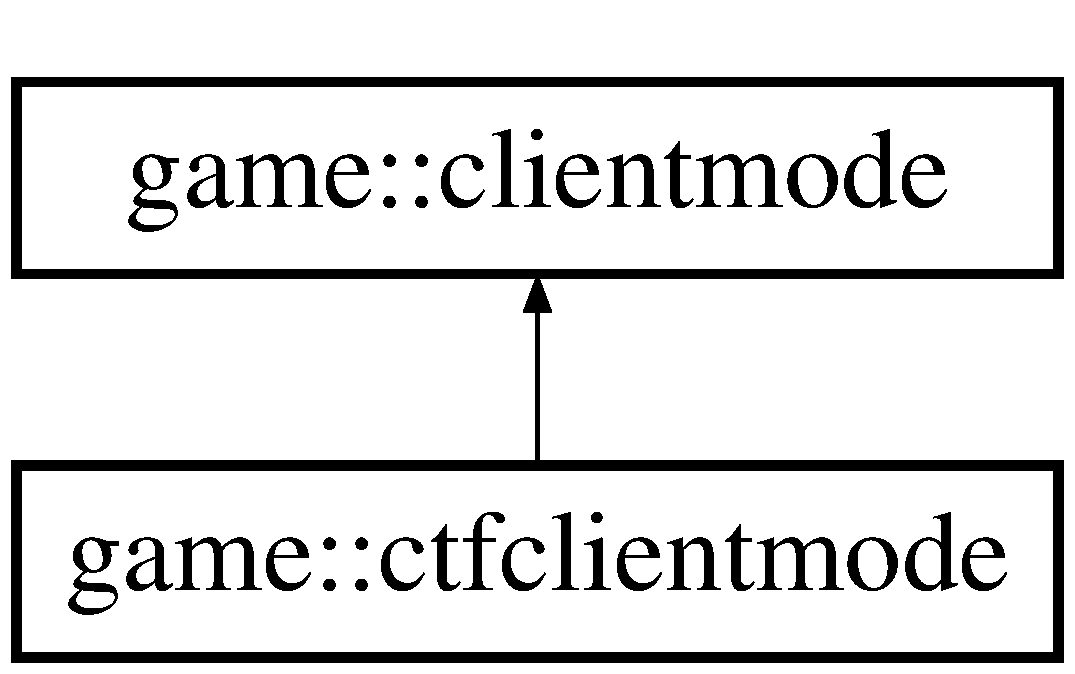
\includegraphics[height=2.000000cm]{structgame_1_1ctfclientmode}
\end{center}
\end{figure}
\subsection*{Classes}
\begin{DoxyCompactItemize}
\item 
struct \hyperlink{structgame_1_1ctfclientmode_1_1flag}{flag}
\end{DoxyCompactItemize}
\subsection*{Public Member Functions}
\begin{DoxyCompactItemize}
\item 
\mbox{\Hypertarget{structgame_1_1ctfclientmode_ae559e772e39b275b8d64d7d321ee6d4d}\label{structgame_1_1ctfclientmode_ae559e772e39b275b8d64d7d321ee6d4d}} 
void {\bfseries resetflags} ()
\item 
\mbox{\Hypertarget{structgame_1_1ctfclientmode_af12db2eff1c5f931c4204e065e5a140c}\label{structgame_1_1ctfclientmode_af12db2eff1c5f931c4204e065e5a140c}} 
bool {\bfseries addflag} (int i, const \hyperlink{structvec}{vec} \&o, int team)
\item 
\mbox{\Hypertarget{structgame_1_1ctfclientmode_af0fb4e25e321eb1ab12eb73f6d3e5cb5}\label{structgame_1_1ctfclientmode_af0fb4e25e321eb1ab12eb73f6d3e5cb5}} 
void {\bfseries ownflag} (int i, \hyperlink{structgameent}{gameent} $\ast$owner, int owntime)
\item 
\mbox{\Hypertarget{structgame_1_1ctfclientmode_aca4eaf4002e7e9f1b13699773b145dcb}\label{structgame_1_1ctfclientmode_aca4eaf4002e7e9f1b13699773b145dcb}} 
void {\bfseries dropflag} (int i, const \hyperlink{structvec}{vec} \&o, float yaw, int droptime)
\item 
\mbox{\Hypertarget{structgame_1_1ctfclientmode_a2427d13dd8670605a77eaae48c7a5075}\label{structgame_1_1ctfclientmode_a2427d13dd8670605a77eaae48c7a5075}} 
void {\bfseries returnflag} (int i)
\item 
\mbox{\Hypertarget{structgame_1_1ctfclientmode_a6693acd9b450ac4e6ae4e81eea0a1dec}\label{structgame_1_1ctfclientmode_a6693acd9b450ac4e6ae4e81eea0a1dec}} 
int {\bfseries totalscore} (int team)
\item 
\mbox{\Hypertarget{structgame_1_1ctfclientmode_ad81bec17a7730a25f5801b94046dea4b}\label{structgame_1_1ctfclientmode_ad81bec17a7730a25f5801b94046dea4b}} 
int {\bfseries setscore} (int team, int score)
\item 
\mbox{\Hypertarget{structgame_1_1ctfclientmode_a4762fbc769b56485a64a53e314f7543f}\label{structgame_1_1ctfclientmode_a4762fbc769b56485a64a53e314f7543f}} 
int {\bfseries addscore} (int team, int score)
\item 
\mbox{\Hypertarget{structgame_1_1ctfclientmode_a4c9b796ab4731441883c300a2842219c}\label{structgame_1_1ctfclientmode_a4c9b796ab4731441883c300a2842219c}} 
bool {\bfseries hidefrags} ()
\item 
\mbox{\Hypertarget{structgame_1_1ctfclientmode_ab5dbd2735af415bcb0a597320c790eaa}\label{structgame_1_1ctfclientmode_ab5dbd2735af415bcb0a597320c790eaa}} 
int {\bfseries getteamscore} (int team)
\item 
\mbox{\Hypertarget{structgame_1_1ctfclientmode_ab7992a1e6f9fb12772da680805f9475b}\label{structgame_1_1ctfclientmode_ab7992a1e6f9fb12772da680805f9475b}} 
void {\bfseries getteamscores} (\hyperlink{structvector}{vector}$<$ \hyperlink{structteamscore}{teamscore} $>$ \&tscores)
\item 
\mbox{\Hypertarget{structgame_1_1ctfclientmode_ad520d9265826fe936033214dc428c7b5}\label{structgame_1_1ctfclientmode_ad520d9265826fe936033214dc428c7b5}} 
void {\bfseries preload} ()
\item 
\mbox{\Hypertarget{structgame_1_1ctfclientmode_a940391bc159c4a12c699d77ef5eb6578}\label{structgame_1_1ctfclientmode_a940391bc159c4a12c699d77ef5eb6578}} 
void {\bfseries drawblip} (\hyperlink{structgameent}{gameent} $\ast$d, float x, float y, float s, const \hyperlink{structvec}{vec} \&pos, bool flagblip)
\item 
\mbox{\Hypertarget{structgame_1_1ctfclientmode_a81452c4cb60058ac5dd7ffb4e674ef38}\label{structgame_1_1ctfclientmode_a81452c4cb60058ac5dd7ffb4e674ef38}} 
void {\bfseries drawblip} (\hyperlink{structgameent}{gameent} $\ast$d, float x, float y, float s, int i, bool flagblip)
\item 
\mbox{\Hypertarget{structgame_1_1ctfclientmode_a606b98f2a28c915e16024aba15db3f3b}\label{structgame_1_1ctfclientmode_a606b98f2a28c915e16024aba15db3f3b}} 
float {\bfseries clipconsole} (float w, float h)
\item 
\mbox{\Hypertarget{structgame_1_1ctfclientmode_a3976554f84e2d260e4da9b3e52567ff2}\label{structgame_1_1ctfclientmode_a3976554f84e2d260e4da9b3e52567ff2}} 
void {\bfseries drawhud} (\hyperlink{structgameent}{gameent} $\ast$d, int w, int h)
\item 
\mbox{\Hypertarget{structgame_1_1ctfclientmode_a6b3d77137c0362115886345b98668229}\label{structgame_1_1ctfclientmode_a6b3d77137c0362115886345b98668229}} 
void {\bfseries removeplayer} (\hyperlink{structgameent}{gameent} $\ast$d)
\item 
\mbox{\Hypertarget{structgame_1_1ctfclientmode_ad93dc199a60060b4df3df677697d09a6}\label{structgame_1_1ctfclientmode_ad93dc199a60060b4df3df677697d09a6}} 
\hyperlink{structvec}{vec} {\bfseries interpflagpos} (\hyperlink{structgame_1_1ctfclientmode_1_1flag}{flag} \&f, float \&angle)
\item 
\mbox{\Hypertarget{structgame_1_1ctfclientmode_aa9bb0e001cef74a9f674044e3721b8c7}\label{structgame_1_1ctfclientmode_aa9bb0e001cef74a9f674044e3721b8c7}} 
\hyperlink{structvec}{vec} {\bfseries interpflagpos} (\hyperlink{structgame_1_1ctfclientmode_1_1flag}{flag} \&f)
\item 
\mbox{\Hypertarget{structgame_1_1ctfclientmode_a158bed55d1473892760d4d3291665540}\label{structgame_1_1ctfclientmode_a158bed55d1473892760d4d3291665540}} 
void {\bfseries rendergame} ()
\item 
\mbox{\Hypertarget{structgame_1_1ctfclientmode_aa372ee6729a5ff42d537cc874d8a0484}\label{structgame_1_1ctfclientmode_aa372ee6729a5ff42d537cc874d8a0484}} 
void {\bfseries setup} ()
\item 
\mbox{\Hypertarget{structgame_1_1ctfclientmode_ad347924d3b4aa89b1a8b2cfb571e2bdd}\label{structgame_1_1ctfclientmode_ad347924d3b4aa89b1a8b2cfb571e2bdd}} 
void {\bfseries senditems} (\hyperlink{structpacketbuf}{packetbuf} \&p)
\item 
\mbox{\Hypertarget{structgame_1_1ctfclientmode_a237724921c8d0a5898d756df83929af7}\label{structgame_1_1ctfclientmode_a237724921c8d0a5898d756df83929af7}} 
void {\bfseries parseflags} (\hyperlink{structdatabuf}{ucharbuf} \&p, bool commit)
\item 
\mbox{\Hypertarget{structgame_1_1ctfclientmode_a2b46979f6ef3167fc76612025c340c97}\label{structgame_1_1ctfclientmode_a2b46979f6ef3167fc76612025c340c97}} 
void {\bfseries trydropflag} ()
\item 
\mbox{\Hypertarget{structgame_1_1ctfclientmode_a408b9f33dafea70d68aee715b95989ec}\label{structgame_1_1ctfclientmode_a408b9f33dafea70d68aee715b95989ec}} 
const char $\ast$ {\bfseries teamcolorflag} (\hyperlink{structgame_1_1ctfclientmode_1_1flag}{flag} \&f)
\item 
\mbox{\Hypertarget{structgame_1_1ctfclientmode_aadf112039a6dfe53727a4257626ec891}\label{structgame_1_1ctfclientmode_aadf112039a6dfe53727a4257626ec891}} 
void {\bfseries dropflag} (\hyperlink{structgameent}{gameent} $\ast$d, int i, int version, const \hyperlink{structvec}{vec} \&droploc)
\item 
\mbox{\Hypertarget{structgame_1_1ctfclientmode_abbde5fc6cc2e13b6275a0e35e63e7e7e}\label{structgame_1_1ctfclientmode_abbde5fc6cc2e13b6275a0e35e63e7e7e}} 
void {\bfseries flagexplosion} (int i, int team, const \hyperlink{structvec}{vec} \&loc)
\item 
\mbox{\Hypertarget{structgame_1_1ctfclientmode_a8e29e3638b16a47f6dfd51db915867f1}\label{structgame_1_1ctfclientmode_a8e29e3638b16a47f6dfd51db915867f1}} 
void {\bfseries flageffect} (int i, int team, const \hyperlink{structvec}{vec} \&from, const \hyperlink{structvec}{vec} \&to)
\item 
\mbox{\Hypertarget{structgame_1_1ctfclientmode_a63ddd1821eea17d153439a90d3f36110}\label{structgame_1_1ctfclientmode_a63ddd1821eea17d153439a90d3f36110}} 
void {\bfseries returnflag} (\hyperlink{structgameent}{gameent} $\ast$d, int i, int version)
\item 
\mbox{\Hypertarget{structgame_1_1ctfclientmode_a3a127acaaeedff336c5673460f05a8ad}\label{structgame_1_1ctfclientmode_a3a127acaaeedff336c5673460f05a8ad}} 
void {\bfseries resetflag} (int i, int version)
\item 
\mbox{\Hypertarget{structgame_1_1ctfclientmode_adb206c4fe3ae24830ac81c61b9858fd8}\label{structgame_1_1ctfclientmode_adb206c4fe3ae24830ac81c61b9858fd8}} 
void {\bfseries scoreflag} (\hyperlink{structgameent}{gameent} $\ast$d, int relay, int relayversion, int goal, int goalversion, int team, int score, int dflags)
\item 
\mbox{\Hypertarget{structgame_1_1ctfclientmode_a04bcae426ddc60c5fc817eac1c872578}\label{structgame_1_1ctfclientmode_a04bcae426ddc60c5fc817eac1c872578}} 
void {\bfseries takeflag} (\hyperlink{structgameent}{gameent} $\ast$d, int i, int version)
\item 
\mbox{\Hypertarget{structgame_1_1ctfclientmode_a90c2ecf1ec35ed4bad13560b1905e979}\label{structgame_1_1ctfclientmode_a90c2ecf1ec35ed4bad13560b1905e979}} 
void {\bfseries checkitems} (\hyperlink{structgameent}{gameent} $\ast$d)
\item 
\mbox{\Hypertarget{structgame_1_1ctfclientmode_a2a8b0caba1dc9a195b8738519bb6d2b5}\label{structgame_1_1ctfclientmode_a2a8b0caba1dc9a195b8738519bb6d2b5}} 
void {\bfseries respawned} (\hyperlink{structgameent}{gameent} $\ast$d)
\item 
\mbox{\Hypertarget{structgame_1_1ctfclientmode_a05652bb6deff45aaa04232b39d9e430e}\label{structgame_1_1ctfclientmode_a05652bb6deff45aaa04232b39d9e430e}} 
int {\bfseries respawnwait} (\hyperlink{structgameent}{gameent} $\ast$d)
\item 
\mbox{\Hypertarget{structgame_1_1ctfclientmode_ae513a1a8863613f18652c983df32a4fe}\label{structgame_1_1ctfclientmode_ae513a1a8863613f18652c983df32a4fe}} 
bool {\bfseries aihomerun} (\hyperlink{structgameent}{gameent} $\ast$d, \hyperlink{structai_1_1aistate}{ai\+::aistate} \&b)
\item 
\mbox{\Hypertarget{structgame_1_1ctfclientmode_a0dc486f7e9cb2854b15012ae9e8f09a7}\label{structgame_1_1ctfclientmode_a0dc486f7e9cb2854b15012ae9e8f09a7}} 
bool {\bfseries aicheck} (\hyperlink{structgameent}{gameent} $\ast$d, \hyperlink{structai_1_1aistate}{ai\+::aistate} \&b)
\item 
\mbox{\Hypertarget{structgame_1_1ctfclientmode_ad5c6c673e6d916889c076049c6d74b4a}\label{structgame_1_1ctfclientmode_ad5c6c673e6d916889c076049c6d74b4a}} 
void {\bfseries aifind} (\hyperlink{structgameent}{gameent} $\ast$d, \hyperlink{structai_1_1aistate}{ai\+::aistate} \&b, \hyperlink{structvector}{vector}$<$ \hyperlink{structai_1_1interest}{ai\+::interest} $>$ \&interests)
\item 
\mbox{\Hypertarget{structgame_1_1ctfclientmode_ac9879571630083b936dff8d16c17365f}\label{structgame_1_1ctfclientmode_ac9879571630083b936dff8d16c17365f}} 
bool {\bfseries aidefend} (\hyperlink{structgameent}{gameent} $\ast$d, \hyperlink{structai_1_1aistate}{ai\+::aistate} \&b)
\item 
\mbox{\Hypertarget{structgame_1_1ctfclientmode_abd8e5581ec9eb7dbe480e1db06112581}\label{structgame_1_1ctfclientmode_abd8e5581ec9eb7dbe480e1db06112581}} 
bool {\bfseries aipursue} (\hyperlink{structgameent}{gameent} $\ast$d, \hyperlink{structai_1_1aistate}{ai\+::aistate} \&b)
\end{DoxyCompactItemize}
\subsection*{Public Attributes}
\begin{DoxyCompactItemize}
\item 
\mbox{\Hypertarget{structgame_1_1ctfclientmode_a37e3b3b1fa51ca28f2eb23b328abe47f}\label{structgame_1_1ctfclientmode_a37e3b3b1fa51ca28f2eb23b328abe47f}} 
\hyperlink{structvector}{vector}$<$ \hyperlink{structgame_1_1ctfclientmode_1_1flag}{flag} $>$ {\bfseries flags}
\item 
\mbox{\Hypertarget{structgame_1_1ctfclientmode_a9ec552f3ec2abc8cf9bdb57f70d4ccdc}\label{structgame_1_1ctfclientmode_a9ec552f3ec2abc8cf9bdb57f70d4ccdc}} 
int {\bfseries scores} \mbox{[}M\+A\+X\+T\+E\+A\+MS\mbox{]}
\end{DoxyCompactItemize}
\subsection*{Static Public Attributes}
\begin{DoxyCompactItemize}
\item 
\mbox{\Hypertarget{structgame_1_1ctfclientmode_aa30e5bca0e905efaaafd4c8b22ffb7ef}\label{structgame_1_1ctfclientmode_aa30e5bca0e905efaaafd4c8b22ffb7ef}} 
static const int {\bfseries M\+A\+X\+F\+L\+A\+GS} = 20
\item 
\mbox{\Hypertarget{structgame_1_1ctfclientmode_a8fb6561710abe3b95a1e7837b2be95b5}\label{structgame_1_1ctfclientmode_a8fb6561710abe3b95a1e7837b2be95b5}} 
static const int {\bfseries F\+L\+A\+G\+R\+A\+D\+I\+US} = 16
\item 
\mbox{\Hypertarget{structgame_1_1ctfclientmode_a7937424bdd8dad980a077b1177a596d5}\label{structgame_1_1ctfclientmode_a7937424bdd8dad980a077b1177a596d5}} 
static const int {\bfseries F\+L\+A\+G\+L\+I\+M\+IT} = 10
\item 
\mbox{\Hypertarget{structgame_1_1ctfclientmode_ab2a85b0a82554ef139149402af7250e7}\label{structgame_1_1ctfclientmode_ab2a85b0a82554ef139149402af7250e7}} 
static const int {\bfseries R\+E\+S\+P\+A\+W\+N\+S\+E\+CS} = 5
\end{DoxyCompactItemize}


The documentation for this struct was generated from the following file\+:\begin{DoxyCompactItemize}
\item 
H\+:/\+Rival\+Engine/\+Rival\+\_\+\+Game\+\_\+\+Engine\+\_\+\+G\+I\+T/\+Rival3dengine/source/game/client.\+cpp\end{DoxyCompactItemize}

\hypertarget{structctfclientmode}{}\section{ctfclientmode Struct Reference}
\label{structctfclientmode}\index{ctfclientmode@{ctfclientmode}}
Inheritance diagram for ctfclientmode\+:\begin{figure}[H]
\begin{center}
\leavevmode
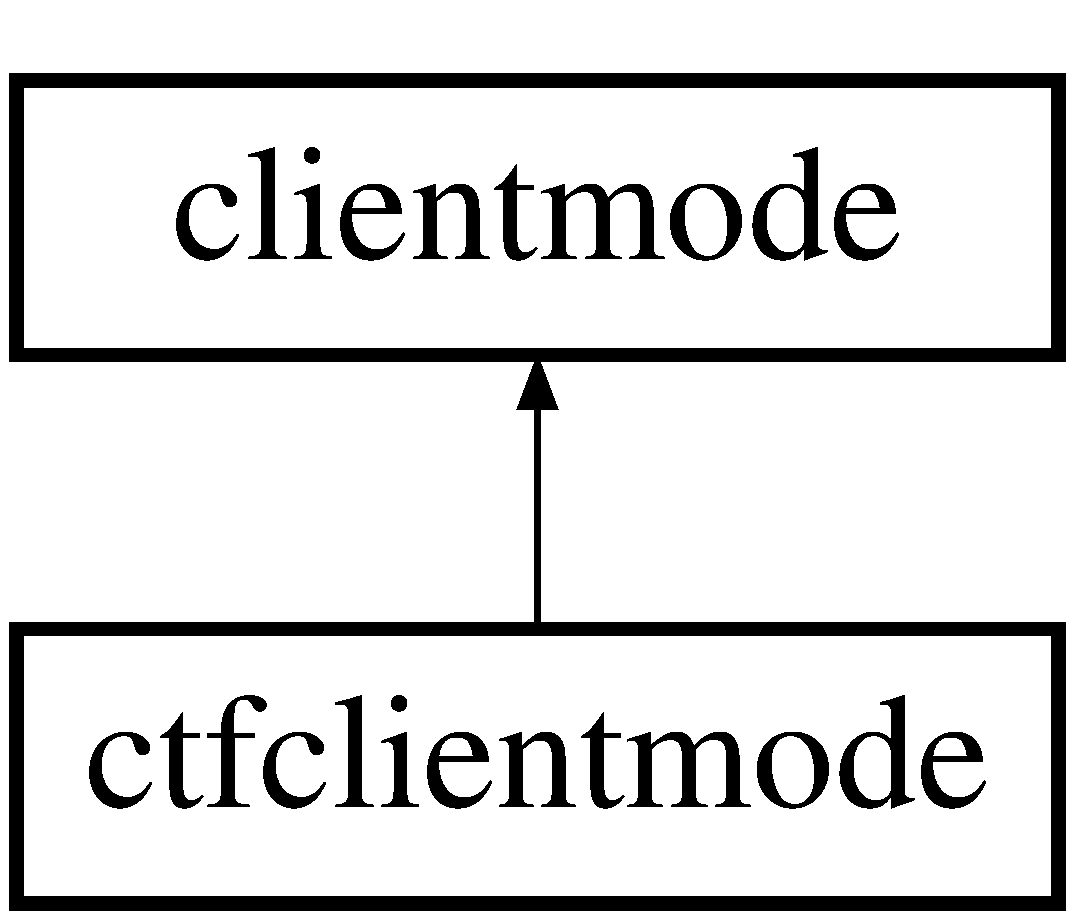
\includegraphics[height=2.000000cm]{structctfclientmode}
\end{center}
\end{figure}
\subsection*{Classes}
\begin{DoxyCompactItemize}
\item 
struct \hyperlink{structctfclientmode_1_1flag}{flag}
\end{DoxyCompactItemize}
\subsection*{Public Member Functions}
\begin{DoxyCompactItemize}
\item 
\mbox{\Hypertarget{structctfclientmode_a6c1da9bcb03d4032a5ead9c9cc86327c}\label{structctfclientmode_a6c1da9bcb03d4032a5ead9c9cc86327c}} 
void {\bfseries resetflags} ()
\item 
\mbox{\Hypertarget{structctfclientmode_ad930aea037d680a90daef807b66a9e7b}\label{structctfclientmode_ad930aea037d680a90daef807b66a9e7b}} 
bool {\bfseries addflag} (int i, const \hyperlink{structvec}{vec} \&o, int team)
\item 
\mbox{\Hypertarget{structctfclientmode_a478c11f516cb0c9dded743377c67f0cf}\label{structctfclientmode_a478c11f516cb0c9dded743377c67f0cf}} 
void {\bfseries ownflag} (int i, \hyperlink{structgameent}{gameent} $\ast$owner, int owntime)
\item 
\mbox{\Hypertarget{structctfclientmode_a1392e2e23e313f77970d8947d4dca259}\label{structctfclientmode_a1392e2e23e313f77970d8947d4dca259}} 
void {\bfseries dropflag} (int i, const \hyperlink{structvec}{vec} \&o, float yaw, int droptime)
\item 
\mbox{\Hypertarget{structctfclientmode_ad63bc73f7c2cf77a626acefbb660fc1e}\label{structctfclientmode_ad63bc73f7c2cf77a626acefbb660fc1e}} 
void {\bfseries returnflag} (int i)
\item 
\mbox{\Hypertarget{structctfclientmode_a45c00c645e223f67757d554ee0da56a9}\label{structctfclientmode_a45c00c645e223f67757d554ee0da56a9}} 
int {\bfseries totalscore} (int team)
\item 
\mbox{\Hypertarget{structctfclientmode_aa0beab2bb8c0d6021cf60ac587c075d9}\label{structctfclientmode_aa0beab2bb8c0d6021cf60ac587c075d9}} 
int {\bfseries setscore} (int team, int score)
\item 
\mbox{\Hypertarget{structctfclientmode_af14fab21e36c62e482aff35a3c105080}\label{structctfclientmode_af14fab21e36c62e482aff35a3c105080}} 
int {\bfseries addscore} (int team, int score)
\item 
\mbox{\Hypertarget{structctfclientmode_a7fc921a21fc97326fea0d0fa212f6bfa}\label{structctfclientmode_a7fc921a21fc97326fea0d0fa212f6bfa}} 
bool {\bfseries hidefrags} ()
\item 
\mbox{\Hypertarget{structctfclientmode_a6f71b234634a9e85dfe2ba483cfa6660}\label{structctfclientmode_a6f71b234634a9e85dfe2ba483cfa6660}} 
int {\bfseries getteamscore} (int team)
\item 
\mbox{\Hypertarget{structctfclientmode_a9ec053925cf13ee85655cbe67db87ac7}\label{structctfclientmode_a9ec053925cf13ee85655cbe67db87ac7}} 
void {\bfseries getteamscores} (\hyperlink{structvector}{vector}$<$ \hyperlink{structteamscore}{teamscore} $>$ \&tscores)
\item 
\mbox{\Hypertarget{structctfclientmode_ac3847c805983e649a11ae5e0c714ff7b}\label{structctfclientmode_ac3847c805983e649a11ae5e0c714ff7b}} 
void {\bfseries preload} ()
\item 
\mbox{\Hypertarget{structctfclientmode_a79a328ae1dcc585380eaaa675b09b4a2}\label{structctfclientmode_a79a328ae1dcc585380eaaa675b09b4a2}} 
void {\bfseries drawblip} (\hyperlink{structgameent}{gameent} $\ast$d, float x, float y, float s, const \hyperlink{structvec}{vec} \&pos, bool flagblip)
\item 
\mbox{\Hypertarget{structctfclientmode_a852c2c18cdd6aeda27ef19943e0e1f25}\label{structctfclientmode_a852c2c18cdd6aeda27ef19943e0e1f25}} 
void {\bfseries drawblip} (\hyperlink{structgameent}{gameent} $\ast$d, float x, float y, float s, int i, bool flagblip)
\item 
\mbox{\Hypertarget{structctfclientmode_aa3fc0c95fa484dd9407a8d901411c3f6}\label{structctfclientmode_aa3fc0c95fa484dd9407a8d901411c3f6}} 
float {\bfseries clipconsole} (float w, float h)
\item 
\mbox{\Hypertarget{structctfclientmode_a6592ac7a3f09f9b7f0287e7c742afc66}\label{structctfclientmode_a6592ac7a3f09f9b7f0287e7c742afc66}} 
void {\bfseries drawhud} (\hyperlink{structgameent}{gameent} $\ast$d, int w, int h)
\item 
\mbox{\Hypertarget{structctfclientmode_ac7c716d3c3fe13bb9362089afb10a4ef}\label{structctfclientmode_ac7c716d3c3fe13bb9362089afb10a4ef}} 
void {\bfseries removeplayer} (\hyperlink{structgameent}{gameent} $\ast$d)
\item 
\mbox{\Hypertarget{structctfclientmode_a0481b45a5094f51e819cf2ee1a91ee58}\label{structctfclientmode_a0481b45a5094f51e819cf2ee1a91ee58}} 
\hyperlink{structvec}{vec} {\bfseries interpflagpos} (\hyperlink{structctfclientmode_1_1flag}{flag} \&f, float \&angle)
\item 
\mbox{\Hypertarget{structctfclientmode_af0219e522caf947e06e43af9ad93892c}\label{structctfclientmode_af0219e522caf947e06e43af9ad93892c}} 
\hyperlink{structvec}{vec} {\bfseries interpflagpos} (\hyperlink{structctfclientmode_1_1flag}{flag} \&f)
\item 
\mbox{\Hypertarget{structctfclientmode_a9bba577b8062a222922dd926e2040f06}\label{structctfclientmode_a9bba577b8062a222922dd926e2040f06}} 
void {\bfseries rendergame} ()
\item 
\mbox{\Hypertarget{structctfclientmode_ae9367ed754802c93ce502fd4cf3b4e2a}\label{structctfclientmode_ae9367ed754802c93ce502fd4cf3b4e2a}} 
void {\bfseries setup} ()
\item 
\mbox{\Hypertarget{structctfclientmode_a19a19ed32f239bbd2097f27868253afd}\label{structctfclientmode_a19a19ed32f239bbd2097f27868253afd}} 
void {\bfseries senditems} (\hyperlink{structpacketbuf}{packetbuf} \&p)
\item 
\mbox{\Hypertarget{structctfclientmode_ab38e92cb8bf9e7c3c78839d7e786d2ba}\label{structctfclientmode_ab38e92cb8bf9e7c3c78839d7e786d2ba}} 
void {\bfseries parseflags} (\hyperlink{structdatabuf}{ucharbuf} \&p, bool commit)
\item 
\mbox{\Hypertarget{structctfclientmode_a8455a8614fbfc82bbca9384f5b1df33d}\label{structctfclientmode_a8455a8614fbfc82bbca9384f5b1df33d}} 
void {\bfseries trydropflag} ()
\item 
\mbox{\Hypertarget{structctfclientmode_a2cad6d40249a404d53ce9b823da31ba4}\label{structctfclientmode_a2cad6d40249a404d53ce9b823da31ba4}} 
const char $\ast$ {\bfseries teamcolorflag} (\hyperlink{structctfclientmode_1_1flag}{flag} \&f)
\item 
\mbox{\Hypertarget{structctfclientmode_a1304cfab3df92b338d2fa1d0913b024b}\label{structctfclientmode_a1304cfab3df92b338d2fa1d0913b024b}} 
void {\bfseries dropflag} (\hyperlink{structgameent}{gameent} $\ast$d, int i, int version, const \hyperlink{structvec}{vec} \&droploc)
\item 
\mbox{\Hypertarget{structctfclientmode_a6f1bbf4c63bf6e8b6c7859a489737ff3}\label{structctfclientmode_a6f1bbf4c63bf6e8b6c7859a489737ff3}} 
void {\bfseries flagexplosion} (int i, int team, const \hyperlink{structvec}{vec} \&loc)
\item 
\mbox{\Hypertarget{structctfclientmode_a3037b6ebbaf617856d3885b07a28c556}\label{structctfclientmode_a3037b6ebbaf617856d3885b07a28c556}} 
void {\bfseries flageffect} (int i, int team, const \hyperlink{structvec}{vec} \&from, const \hyperlink{structvec}{vec} \&to)
\item 
\mbox{\Hypertarget{structctfclientmode_a564fea7dd03377b5b71a80c4405c9906}\label{structctfclientmode_a564fea7dd03377b5b71a80c4405c9906}} 
void {\bfseries returnflag} (\hyperlink{structgameent}{gameent} $\ast$d, int i, int version)
\item 
\mbox{\Hypertarget{structctfclientmode_a96f10b771db1011a9859933e5769acf7}\label{structctfclientmode_a96f10b771db1011a9859933e5769acf7}} 
void {\bfseries resetflag} (int i, int version)
\item 
\mbox{\Hypertarget{structctfclientmode_a2cdc56863992c99ce8f770bd7b89af3c}\label{structctfclientmode_a2cdc56863992c99ce8f770bd7b89af3c}} 
void {\bfseries scoreflag} (\hyperlink{structgameent}{gameent} $\ast$d, int relay, int relayversion, int goal, int goalversion, int team, int score, int dflags)
\item 
\mbox{\Hypertarget{structctfclientmode_aadd04582ad24796437b9a6b3d33436bd}\label{structctfclientmode_aadd04582ad24796437b9a6b3d33436bd}} 
void {\bfseries takeflag} (\hyperlink{structgameent}{gameent} $\ast$d, int i, int version)
\item 
\mbox{\Hypertarget{structctfclientmode_a121eda171cadb8f07283d96dafaf1b5c}\label{structctfclientmode_a121eda171cadb8f07283d96dafaf1b5c}} 
void {\bfseries checkitems} (\hyperlink{structgameent}{gameent} $\ast$d)
\item 
\mbox{\Hypertarget{structctfclientmode_a8baa46f221c027ab6a0c7fcf1c10b0df}\label{structctfclientmode_a8baa46f221c027ab6a0c7fcf1c10b0df}} 
void {\bfseries respawned} (\hyperlink{structgameent}{gameent} $\ast$d)
\item 
\mbox{\Hypertarget{structctfclientmode_a91e1fa701790d4fadd989270f43f82e5}\label{structctfclientmode_a91e1fa701790d4fadd989270f43f82e5}} 
int {\bfseries respawnwait} (\hyperlink{structgameent}{gameent} $\ast$d)
\item 
\mbox{\Hypertarget{structctfclientmode_a08bc510c01a160bdc1866759de0ae593}\label{structctfclientmode_a08bc510c01a160bdc1866759de0ae593}} 
bool {\bfseries aihomerun} (\hyperlink{structgameent}{gameent} $\ast$d, \hyperlink{structai_1_1aistate}{ai\+::aistate} \&b)
\item 
\mbox{\Hypertarget{structctfclientmode_a6f5742a1572cc75218a26779abf89d19}\label{structctfclientmode_a6f5742a1572cc75218a26779abf89d19}} 
bool {\bfseries aicheck} (\hyperlink{structgameent}{gameent} $\ast$d, \hyperlink{structai_1_1aistate}{ai\+::aistate} \&b)
\item 
\mbox{\Hypertarget{structctfclientmode_a1affaf006ae7e9707ad028c4e25ad80a}\label{structctfclientmode_a1affaf006ae7e9707ad028c4e25ad80a}} 
void {\bfseries aifind} (\hyperlink{structgameent}{gameent} $\ast$d, \hyperlink{structai_1_1aistate}{ai\+::aistate} \&b, \hyperlink{structvector}{vector}$<$ \hyperlink{structai_1_1interest}{ai\+::interest} $>$ \&interests)
\item 
\mbox{\Hypertarget{structctfclientmode_a5b4bb6bf9553dffecaf1654ddd7bb791}\label{structctfclientmode_a5b4bb6bf9553dffecaf1654ddd7bb791}} 
bool {\bfseries aidefend} (\hyperlink{structgameent}{gameent} $\ast$d, \hyperlink{structai_1_1aistate}{ai\+::aistate} \&b)
\item 
\mbox{\Hypertarget{structctfclientmode_a3c8ef295a3df44919aca35b77d2ad7d3}\label{structctfclientmode_a3c8ef295a3df44919aca35b77d2ad7d3}} 
bool {\bfseries aipursue} (\hyperlink{structgameent}{gameent} $\ast$d, \hyperlink{structai_1_1aistate}{ai\+::aistate} \&b)
\end{DoxyCompactItemize}
\subsection*{Public Attributes}
\begin{DoxyCompactItemize}
\item 
\mbox{\Hypertarget{structctfclientmode_a54da7b616182daded9fb8e82267b481e}\label{structctfclientmode_a54da7b616182daded9fb8e82267b481e}} 
\hyperlink{structvector}{vector}$<$ \hyperlink{structctfclientmode_1_1flag}{flag} $>$ {\bfseries flags}
\item 
\mbox{\Hypertarget{structctfclientmode_a00ccd042ee47e728f613671bb40119d1}\label{structctfclientmode_a00ccd042ee47e728f613671bb40119d1}} 
int {\bfseries scores} \mbox{[}M\+A\+X\+T\+E\+A\+MS\mbox{]}
\end{DoxyCompactItemize}
\subsection*{Static Public Attributes}
\begin{DoxyCompactItemize}
\item 
\mbox{\Hypertarget{structctfclientmode_af2efca7d9ca5b0b4eaeb4930b0f436c2}\label{structctfclientmode_af2efca7d9ca5b0b4eaeb4930b0f436c2}} 
static const int {\bfseries M\+A\+X\+F\+L\+A\+GS} = 20
\item 
\mbox{\Hypertarget{structctfclientmode_a9ce81e5ddf40a4829f25635e747673a3}\label{structctfclientmode_a9ce81e5ddf40a4829f25635e747673a3}} 
static const int {\bfseries F\+L\+A\+G\+R\+A\+D\+I\+US} = 16
\item 
\mbox{\Hypertarget{structctfclientmode_ac4dc1e4b9e23e4a1be6a24deee26b862}\label{structctfclientmode_ac4dc1e4b9e23e4a1be6a24deee26b862}} 
static const int {\bfseries F\+L\+A\+G\+L\+I\+M\+IT} = 10
\item 
\mbox{\Hypertarget{structctfclientmode_abe294eee06da4ef0c433988ef751c4a5}\label{structctfclientmode_abe294eee06da4ef0c433988ef751c4a5}} 
static const int {\bfseries R\+E\+S\+P\+A\+W\+N\+S\+E\+CS} = 5
\end{DoxyCompactItemize}


The documentation for this struct was generated from the following file\+:\begin{DoxyCompactItemize}
\item 
H\+:/\+Rival\+Engine/\+Rival\+\_\+\+Game\+\_\+\+Engine\+\_\+\+G\+I\+T/\+Rival3dengine/source/game/ctf.\+h\end{DoxyCompactItemize}

\hypertarget{structserver_1_1ctfservmode}{}\section{server\+:\+:ctfservmode Struct Reference}
\label{structserver_1_1ctfservmode}\index{server\+::ctfservmode@{server\+::ctfservmode}}
Inheritance diagram for server\+:\+:ctfservmode\+:\begin{figure}[H]
\begin{center}
\leavevmode
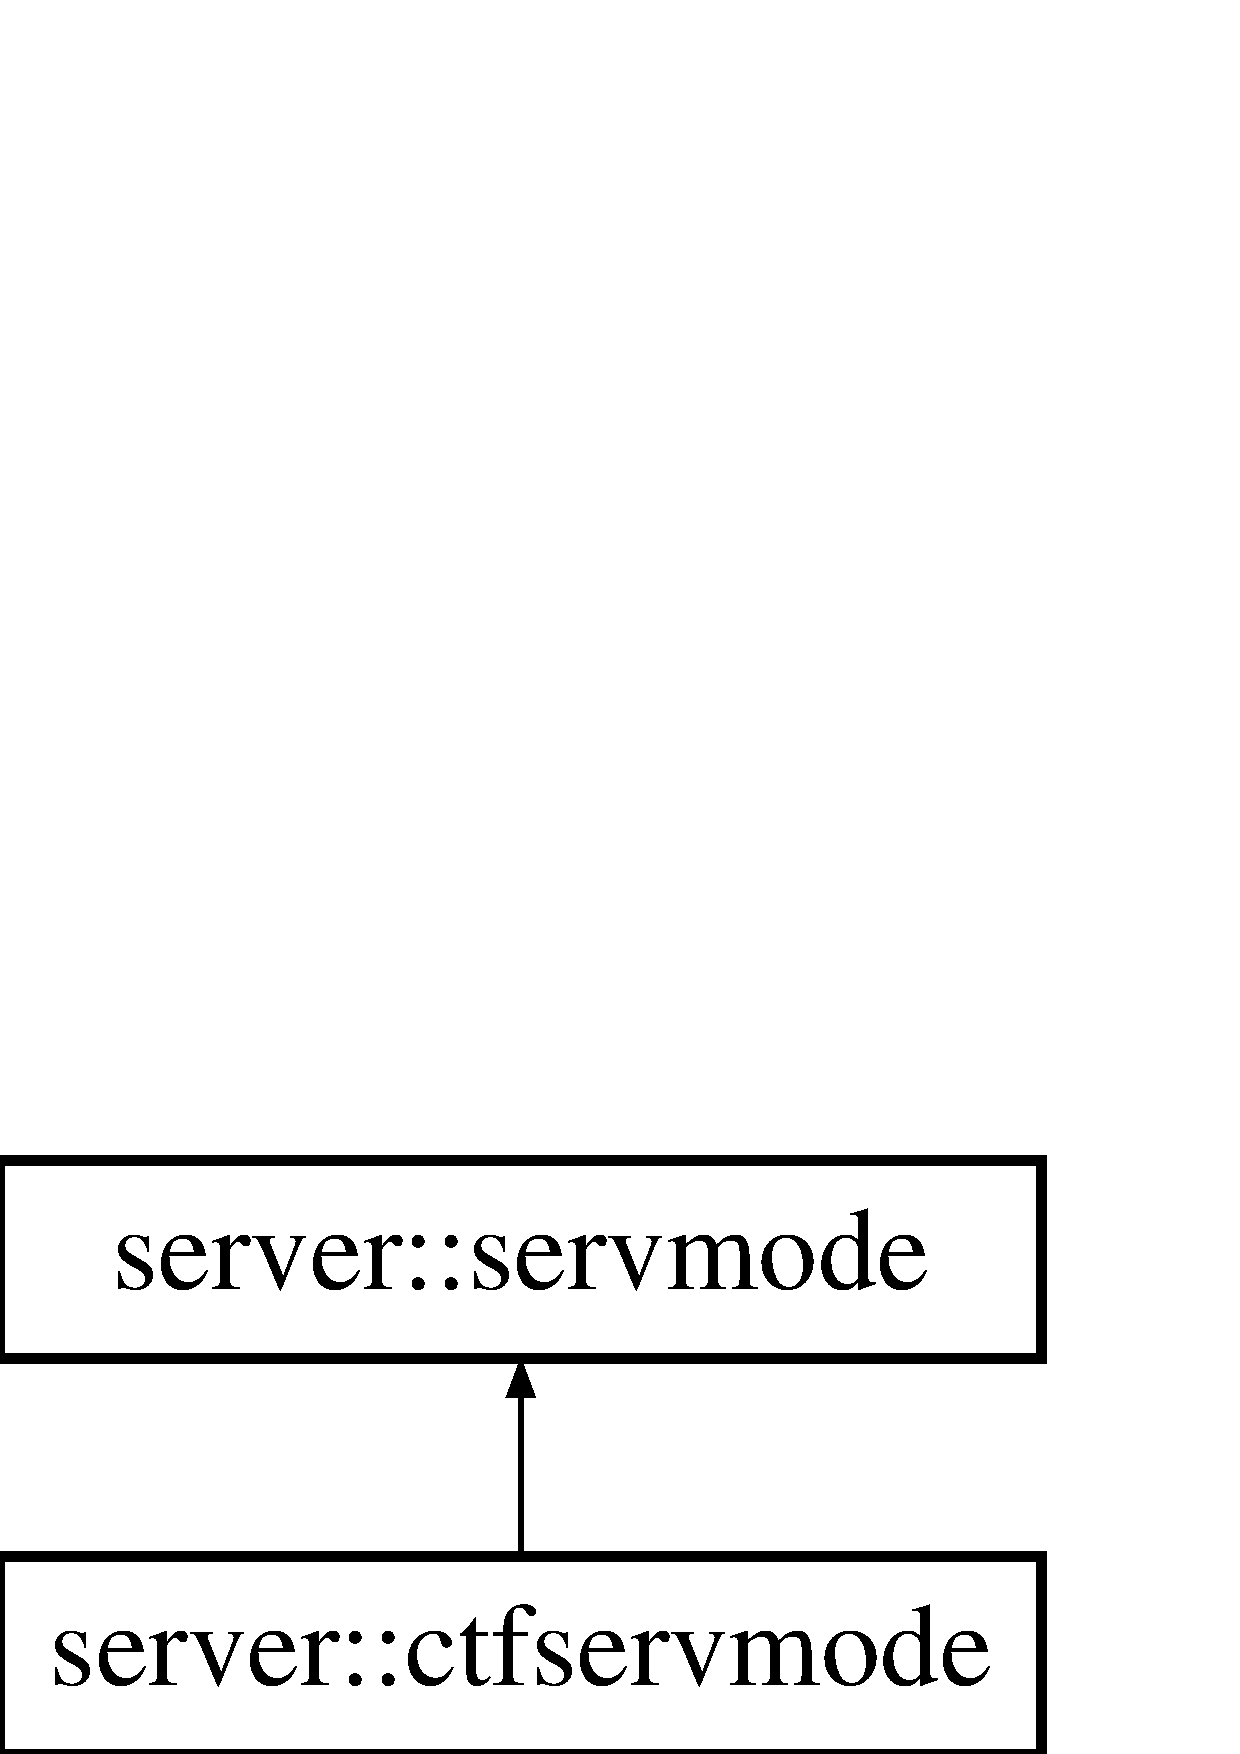
\includegraphics[height=2.000000cm]{structserver_1_1ctfservmode}
\end{center}
\end{figure}
\subsection*{Classes}
\begin{DoxyCompactItemize}
\item 
struct \hyperlink{structserver_1_1ctfservmode_1_1flag}{flag}
\end{DoxyCompactItemize}
\subsection*{Public Member Functions}
\begin{DoxyCompactItemize}
\item 
\mbox{\Hypertarget{structserver_1_1ctfservmode_abb48efb6b5dd5e20d487f0828f8ed311}\label{structserver_1_1ctfservmode_abb48efb6b5dd5e20d487f0828f8ed311}} 
void {\bfseries resetflags} ()
\item 
\mbox{\Hypertarget{structserver_1_1ctfservmode_a1d73a0c7460d2d74788e7867e4a38301}\label{structserver_1_1ctfservmode_a1d73a0c7460d2d74788e7867e4a38301}} 
bool {\bfseries addflag} (int i, const \hyperlink{structvec}{vec} \&o, int team)
\item 
\mbox{\Hypertarget{structserver_1_1ctfservmode_a5bbf56cb81f3727efbdfe59c2d86e971}\label{structserver_1_1ctfservmode_a5bbf56cb81f3727efbdfe59c2d86e971}} 
void {\bfseries ownflag} (int i, int owner, int owntime)
\item 
\mbox{\Hypertarget{structserver_1_1ctfservmode_adaf6e4bbfa047ae3d83f20377286a03a}\label{structserver_1_1ctfservmode_adaf6e4bbfa047ae3d83f20377286a03a}} 
void {\bfseries dropflag} (int i, const \hyperlink{structvec}{vec} \&o, int droptime, int dropper=-\/1, bool penalty=false)
\item 
\mbox{\Hypertarget{structserver_1_1ctfservmode_a445e1d4be77b7b01bc6535c78a8276ec}\label{structserver_1_1ctfservmode_a445e1d4be77b7b01bc6535c78a8276ec}} 
void {\bfseries returnflag} (int i)
\item 
\mbox{\Hypertarget{structserver_1_1ctfservmode_a39003e9b247deb2b0a26dce9d65717ff}\label{structserver_1_1ctfservmode_a39003e9b247deb2b0a26dce9d65717ff}} 
int {\bfseries totalscore} (int team)
\item 
\mbox{\Hypertarget{structserver_1_1ctfservmode_a77cffdac6b3f78827ebd6e897a29f07b}\label{structserver_1_1ctfservmode_a77cffdac6b3f78827ebd6e897a29f07b}} 
int {\bfseries setscore} (int team, int score)
\item 
\mbox{\Hypertarget{structserver_1_1ctfservmode_a1e70feb67367d6bd4a9f6176e582de32}\label{structserver_1_1ctfservmode_a1e70feb67367d6bd4a9f6176e582de32}} 
int {\bfseries addscore} (int team, int score)
\item 
\mbox{\Hypertarget{structserver_1_1ctfservmode_a638ef439347a831bf057c3f47b6731c1}\label{structserver_1_1ctfservmode_a638ef439347a831bf057c3f47b6731c1}} 
bool {\bfseries hidefrags} ()
\item 
\mbox{\Hypertarget{structserver_1_1ctfservmode_aa823a313493bc40e07102a3a6294d604}\label{structserver_1_1ctfservmode_aa823a313493bc40e07102a3a6294d604}} 
int {\bfseries getteamscore} (int team)
\item 
\mbox{\Hypertarget{structserver_1_1ctfservmode_a17479447cf0518ea91edfc4367035c51}\label{structserver_1_1ctfservmode_a17479447cf0518ea91edfc4367035c51}} 
void {\bfseries getteamscores} (\hyperlink{structvector}{vector}$<$ \hyperlink{structteamscore}{teamscore} $>$ \&tscores)
\item 
\mbox{\Hypertarget{structserver_1_1ctfservmode_af1b49e2f8b12307e915f078e62fd979b}\label{structserver_1_1ctfservmode_af1b49e2f8b12307e915f078e62fd979b}} 
void {\bfseries reset} (bool empty)
\item 
\mbox{\Hypertarget{structserver_1_1ctfservmode_a69ba29c34c11f73a76a7aa372f235cfd}\label{structserver_1_1ctfservmode_a69ba29c34c11f73a76a7aa372f235cfd}} 
void {\bfseries cleanup} ()
\item 
\mbox{\Hypertarget{structserver_1_1ctfservmode_a6490922a50b76043f35993350e3c712b}\label{structserver_1_1ctfservmode_a6490922a50b76043f35993350e3c712b}} 
void {\bfseries setup} ()
\item 
\mbox{\Hypertarget{structserver_1_1ctfservmode_a7239fd7509a43ddcbc05c2264ff898a2}\label{structserver_1_1ctfservmode_a7239fd7509a43ddcbc05c2264ff898a2}} 
void {\bfseries newmap} ()
\item 
\mbox{\Hypertarget{structserver_1_1ctfservmode_aa452a428fbae2d8f1182f482f47bd2b4}\label{structserver_1_1ctfservmode_aa452a428fbae2d8f1182f482f47bd2b4}} 
void {\bfseries dropflag} (\hyperlink{structserver_1_1clientinfo}{clientinfo} $\ast$ci, \hyperlink{structserver_1_1clientinfo}{clientinfo} $\ast$dropper=N\+U\+LL)
\item 
\mbox{\Hypertarget{structserver_1_1ctfservmode_a78edfb53f86a8cb687977a7c5493b6c7}\label{structserver_1_1ctfservmode_a78edfb53f86a8cb687977a7c5493b6c7}} 
void {\bfseries leavegame} (\hyperlink{structserver_1_1clientinfo}{clientinfo} $\ast$ci, bool disconnecting=false)
\item 
\mbox{\Hypertarget{structserver_1_1ctfservmode_ac0cac6be41bd475f7b0235b5329c1411}\label{structserver_1_1ctfservmode_ac0cac6be41bd475f7b0235b5329c1411}} 
void {\bfseries died} (\hyperlink{structserver_1_1clientinfo}{clientinfo} $\ast$ci, \hyperlink{structserver_1_1clientinfo}{clientinfo} $\ast$actor)
\item 
\mbox{\Hypertarget{structserver_1_1ctfservmode_aed1a20b5fdab14d664f7c257783ef28d}\label{structserver_1_1ctfservmode_aed1a20b5fdab14d664f7c257783ef28d}} 
bool {\bfseries canspawn} (\hyperlink{structserver_1_1clientinfo}{clientinfo} $\ast$ci, bool connecting)
\item 
\mbox{\Hypertarget{structserver_1_1ctfservmode_ace8ad4b56e8763e7227a58511d19617c}\label{structserver_1_1ctfservmode_ace8ad4b56e8763e7227a58511d19617c}} 
bool {\bfseries canchangeteam} (\hyperlink{structserver_1_1clientinfo}{clientinfo} $\ast$ci, int oldteam, int newteam)
\item 
\mbox{\Hypertarget{structserver_1_1ctfservmode_a8c5e5155e6cfb7956c460ffcdf2955b1}\label{structserver_1_1ctfservmode_a8c5e5155e6cfb7956c460ffcdf2955b1}} 
void {\bfseries changeteam} (\hyperlink{structserver_1_1clientinfo}{clientinfo} $\ast$ci, int oldteam, int newteam)
\item 
\mbox{\Hypertarget{structserver_1_1ctfservmode_a56f00670fe165ee35413d3a6debe5dd2}\label{structserver_1_1ctfservmode_a56f00670fe165ee35413d3a6debe5dd2}} 
void {\bfseries scoreflag} (\hyperlink{structserver_1_1clientinfo}{clientinfo} $\ast$ci, int goal, int relay=-\/1)
\item 
\mbox{\Hypertarget{structserver_1_1ctfservmode_ab0dfb3594347f3e282d589e53a5b7068}\label{structserver_1_1ctfservmode_ab0dfb3594347f3e282d589e53a5b7068}} 
void {\bfseries takeflag} (\hyperlink{structserver_1_1clientinfo}{clientinfo} $\ast$ci, int i, int version)
\item 
\mbox{\Hypertarget{structserver_1_1ctfservmode_a41c651d043609f8633323e698288a820}\label{structserver_1_1ctfservmode_a41c651d043609f8633323e698288a820}} 
void {\bfseries update} ()
\item 
\mbox{\Hypertarget{structserver_1_1ctfservmode_af95ad62d23a9b295cfcac8a9ea96ba40}\label{structserver_1_1ctfservmode_af95ad62d23a9b295cfcac8a9ea96ba40}} 
void {\bfseries initclient} (\hyperlink{structserver_1_1clientinfo}{clientinfo} $\ast$ci, \hyperlink{structpacketbuf}{packetbuf} \&p, bool connecting)
\item 
\mbox{\Hypertarget{structserver_1_1ctfservmode_a5b62660b25ef739a6ebbb9f024f9a07a}\label{structserver_1_1ctfservmode_a5b62660b25ef739a6ebbb9f024f9a07a}} 
void {\bfseries parseflags} (\hyperlink{structdatabuf}{ucharbuf} \&p, bool commit)
\end{DoxyCompactItemize}
\subsection*{Public Attributes}
\begin{DoxyCompactItemize}
\item 
\mbox{\Hypertarget{structserver_1_1ctfservmode_a1271874f869c6d33c6d8186c9e26693b}\label{structserver_1_1ctfservmode_a1271874f869c6d33c6d8186c9e26693b}} 
\hyperlink{structvector}{vector}$<$ \hyperlink{structserver_1_1ctfservmode_1_1flag}{flag} $>$ {\bfseries flags}
\item 
\mbox{\Hypertarget{structserver_1_1ctfservmode_a99ea10d6fe1fc0f82bb78a546f156ad1}\label{structserver_1_1ctfservmode_a99ea10d6fe1fc0f82bb78a546f156ad1}} 
int {\bfseries scores} \mbox{[}M\+A\+X\+T\+E\+A\+MS\mbox{]}
\item 
\mbox{\Hypertarget{structserver_1_1ctfservmode_a62bab7c9273c7e72ee4de5d17c6aebdc}\label{structserver_1_1ctfservmode_a62bab7c9273c7e72ee4de5d17c6aebdc}} 
bool {\bfseries notgotflags}
\end{DoxyCompactItemize}
\subsection*{Static Public Attributes}
\begin{DoxyCompactItemize}
\item 
\mbox{\Hypertarget{structserver_1_1ctfservmode_a7b9a05fd211dc9631c16aae8c3273a7f}\label{structserver_1_1ctfservmode_a7b9a05fd211dc9631c16aae8c3273a7f}} 
static const int {\bfseries M\+A\+X\+F\+L\+A\+GS} = 20
\item 
\mbox{\Hypertarget{structserver_1_1ctfservmode_a82d87cfdc4f08784c0fe6efe30ce1a9d}\label{structserver_1_1ctfservmode_a82d87cfdc4f08784c0fe6efe30ce1a9d}} 
static const int {\bfseries F\+L\+A\+G\+R\+A\+D\+I\+US} = 16
\item 
\mbox{\Hypertarget{structserver_1_1ctfservmode_ac32e856f76d99823ad5ae2ae58f3ba48}\label{structserver_1_1ctfservmode_ac32e856f76d99823ad5ae2ae58f3ba48}} 
static const int {\bfseries F\+L\+A\+G\+L\+I\+M\+IT} = 10
\item 
\mbox{\Hypertarget{structserver_1_1ctfservmode_ad8fd3c49f1c8582019b35ca0772f677a}\label{structserver_1_1ctfservmode_ad8fd3c49f1c8582019b35ca0772f677a}} 
static const int {\bfseries R\+E\+S\+P\+A\+W\+N\+S\+E\+CS} = 5
\item 
\mbox{\Hypertarget{structserver_1_1ctfservmode_a9e44b6f1f6712720c78d2cc16f120ee4}\label{structserver_1_1ctfservmode_a9e44b6f1f6712720c78d2cc16f120ee4}} 
static const int {\bfseries R\+E\+S\+E\+T\+F\+L\+A\+G\+T\+I\+ME} = 10000
\end{DoxyCompactItemize}


The documentation for this struct was generated from the following file\+:\begin{DoxyCompactItemize}
\item 
H\+:/\+Rival\+Engine/\+Rival\+\_\+\+Game\+\_\+\+Engine\+\_\+\+G\+I\+T/\+Rival3dengine/source/game/server.\+cpp\end{DoxyCompactItemize}

\hypertarget{structcube}{}\section{cube Struct Reference}
\label{structcube}\index{cube@{cube}}


Inherited by emptycube.

\subsection*{Public Attributes}
\begin{DoxyCompactItemize}
\item 
\mbox{\Hypertarget{structcube_aafb02cf1aa0596ea8677b84654da9e79}\label{structcube_aafb02cf1aa0596ea8677b84654da9e79}} 
\hyperlink{structcube}{cube} $\ast$ {\bfseries children}
\item 
\mbox{\Hypertarget{structcube_a6369b99225574ebfc5e4806004492f21}\label{structcube_a6369b99225574ebfc5e4806004492f21}} 
\hyperlink{structcubeext}{cubeext} $\ast$ {\bfseries ext}
\item 
\mbox{\Hypertarget{structcube_a7a1b12cae3c23f9df97683de0d1e62ea}\label{structcube_a7a1b12cae3c23f9df97683de0d1e62ea}} 
\begin{tabbing}
xx\=xx\=xx\=xx\=xx\=xx\=xx\=xx\=xx\=\kill
union \{\\
\>uchar {\bfseries edges} \mbox{[}12\mbox{]}\\
\>uint {\bfseries faces} \mbox{[}3\mbox{]}\\
\}; \\

\end{tabbing}\item 
\mbox{\Hypertarget{structcube_afd1fe0c107339a3c20060cda213b8aa5}\label{structcube_afd1fe0c107339a3c20060cda213b8aa5}} 
ushort {\bfseries texture} \mbox{[}6\mbox{]}
\item 
\mbox{\Hypertarget{structcube_adabf7826306d245930ea049e0a8bf76e}\label{structcube_adabf7826306d245930ea049e0a8bf76e}} 
ushort {\bfseries material}
\item 
\mbox{\Hypertarget{structcube_a715d3e7eef34036806eaa216a36afdbe}\label{structcube_a715d3e7eef34036806eaa216a36afdbe}} 
uchar {\bfseries merged}
\item 
\mbox{\Hypertarget{structcube_a19df9808564c30c7529e8f9af2431320}\label{structcube_a19df9808564c30c7529e8f9af2431320}} 
\begin{tabbing}
xx\=xx\=xx\=xx\=xx\=xx\=xx\=xx\=xx\=\kill
union \{\\
\>uchar {\bfseries escaped}\\
\>uchar {\bfseries visible}\\
\}; \\

\end{tabbing}\end{DoxyCompactItemize}


The documentation for this struct was generated from the following file\+:\begin{DoxyCompactItemize}
\item 
H\+:/\+Rival\+Engine/\+Rival\+\_\+\+Game\+\_\+\+Engine\+\_\+\+G\+I\+T/\+Rival3dengine/source/engine/octa.\+h\end{DoxyCompactItemize}

\hypertarget{structcubeedge}{}\section{cubeedge Struct Reference}
\label{structcubeedge}\index{cubeedge@{cubeedge}}
\subsection*{Public Attributes}
\begin{DoxyCompactItemize}
\item 
\mbox{\Hypertarget{structcubeedge_ac43ae7f8950a49f658c33120e053af81}\label{structcubeedge_ac43ae7f8950a49f658c33120e053af81}} 
\hyperlink{structcube}{cube} $\ast$ {\bfseries c}
\item 
\mbox{\Hypertarget{structcubeedge_a5efd0446276720a6d155bfff33d1f9bd}\label{structcubeedge_a5efd0446276720a6d155bfff33d1f9bd}} 
int {\bfseries next}
\item 
\mbox{\Hypertarget{structcubeedge_a61b6c1edc1c08ccda653d5edad344c2b}\label{structcubeedge_a61b6c1edc1c08ccda653d5edad344c2b}} 
int {\bfseries offset}
\item 
\mbox{\Hypertarget{structcubeedge_ac9d6ca98e013cfe7c15a283d621cae1c}\label{structcubeedge_ac9d6ca98e013cfe7c15a283d621cae1c}} 
ushort {\bfseries size}
\item 
\mbox{\Hypertarget{structcubeedge_abcf8b1a174f390ef9f47b3ecfa2b440e}\label{structcubeedge_abcf8b1a174f390ef9f47b3ecfa2b440e}} 
uchar {\bfseries index}
\item 
\mbox{\Hypertarget{structcubeedge_a95d7f0b418b776ce6c30741443d76585}\label{structcubeedge_a95d7f0b418b776ce6c30741443d76585}} 
uchar {\bfseries flags}
\end{DoxyCompactItemize}


The documentation for this struct was generated from the following file\+:\begin{DoxyCompactItemize}
\item 
H\+:/\+Rival\+Engine/\+Rival\+\_\+\+Game\+\_\+\+Engine\+\_\+\+G\+I\+T/\+Rival3dengine/source/engine/octarender.\+cpp\end{DoxyCompactItemize}

\hypertarget{structcubeext}{}\section{cubeext Struct Reference}
\label{structcubeext}\index{cubeext@{cubeext}}
\subsection*{Public Member Functions}
\begin{DoxyCompactItemize}
\item 
\mbox{\Hypertarget{structcubeext_adc92712b47146c4aafb2e030b8275b23}\label{structcubeext_adc92712b47146c4aafb2e030b8275b23}} 
\hyperlink{structvertinfo}{vertinfo} $\ast$ {\bfseries verts} ()
\end{DoxyCompactItemize}
\subsection*{Public Attributes}
\begin{DoxyCompactItemize}
\item 
\mbox{\Hypertarget{structcubeext_a126ac675e7d3f34953f046f9f329f8e3}\label{structcubeext_a126ac675e7d3f34953f046f9f329f8e3}} 
\hyperlink{structvtxarray}{vtxarray} $\ast$ {\bfseries va}
\item 
\mbox{\Hypertarget{structcubeext_aefebd2583240fe66f9a35f4d4d742dc1}\label{structcubeext_aefebd2583240fe66f9a35f4d4d742dc1}} 
\hyperlink{structoctaentities}{octaentities} $\ast$ {\bfseries ents}
\item 
\mbox{\Hypertarget{structcubeext_a2c778df7ae4b2c6606a8396d06604769}\label{structcubeext_a2c778df7ae4b2c6606a8396d06604769}} 
\hyperlink{structsurfaceinfo}{surfaceinfo} {\bfseries surfaces} \mbox{[}6\mbox{]}
\item 
\mbox{\Hypertarget{structcubeext_a2507cea49955710785ea9bdf8de4fff7}\label{structcubeext_a2507cea49955710785ea9bdf8de4fff7}} 
int {\bfseries tjoints}
\item 
\mbox{\Hypertarget{structcubeext_a09a7f8f515ef1c0108bc98a4d5682612}\label{structcubeext_a09a7f8f515ef1c0108bc98a4d5682612}} 
uchar {\bfseries maxverts}
\end{DoxyCompactItemize}


The documentation for this struct was generated from the following file\+:\begin{DoxyCompactItemize}
\item 
H\+:/\+Rival\+Engine/\+Rival\+\_\+\+Game\+\_\+\+Engine\+\_\+\+G\+I\+T/\+Rival3dengine/source/engine/octa.\+h\end{DoxyCompactItemize}

\hypertarget{structcubemapside}{}\section{cubemapside Struct Reference}
\label{structcubemapside}\index{cubemapside@{cubemapside}}
\subsection*{Public Attributes}
\begin{DoxyCompactItemize}
\item 
\mbox{\Hypertarget{structcubemapside_a09dd5d5bf09b6a585248a65f766ab304}\label{structcubemapside_a09dd5d5bf09b6a585248a65f766ab304}} 
G\+Lenum {\bfseries target}
\item 
\mbox{\Hypertarget{structcubemapside_a96675f8f5a73627b3eac591b9efd1379}\label{structcubemapside_a96675f8f5a73627b3eac591b9efd1379}} 
const char $\ast$ {\bfseries name}
\item 
\mbox{\Hypertarget{structcubemapside_a2775d224ad79cadb7f05e92be66e18d8}\label{structcubemapside_a2775d224ad79cadb7f05e92be66e18d8}} 
bool {\bfseries flipx}
\item 
\mbox{\Hypertarget{structcubemapside_ad40e1cae16eaa4856fad3d282d051f9d}\label{structcubemapside_ad40e1cae16eaa4856fad3d282d051f9d}} 
bool {\bfseries flipy}
\item 
\mbox{\Hypertarget{structcubemapside_a3078f25f9eb10b373ea4953efb1d06e4}\label{structcubemapside_a3078f25f9eb10b373ea4953efb1d06e4}} 
bool {\bfseries swapxy}
\end{DoxyCompactItemize}


The documentation for this struct was generated from the following file\+:\begin{DoxyCompactItemize}
\item 
H\+:/\+Rival\+Engine/\+Rival\+\_\+\+Game\+\_\+\+Engine\+\_\+\+G\+I\+T/\+Rival3dengine/source/engine/texture.\+h\end{DoxyCompactItemize}

\hypertarget{structmpr_1_1_cube_planes}{}\section{mpr\+:\+:Cube\+Planes Struct Reference}
\label{structmpr_1_1_cube_planes}\index{mpr\+::\+Cube\+Planes@{mpr\+::\+Cube\+Planes}}
\subsection*{Public Member Functions}
\begin{DoxyCompactItemize}
\item 
\mbox{\Hypertarget{structmpr_1_1_cube_planes_ae7449b116f141ab759caa8c165ba4cf9}\label{structmpr_1_1_cube_planes_ae7449b116f141ab759caa8c165ba4cf9}} 
{\bfseries Cube\+Planes} (const \hyperlink{structclipplanes}{clipplanes} \&p)
\item 
\mbox{\Hypertarget{structmpr_1_1_cube_planes_affdb7130f5b9aac9e02383178b2228b6}\label{structmpr_1_1_cube_planes_affdb7130f5b9aac9e02383178b2228b6}} 
\hyperlink{structvec}{vec} {\bfseries center} () const
\item 
\mbox{\Hypertarget{structmpr_1_1_cube_planes_afa39bf3c3c76ea0bb9b980596377cf1d}\label{structmpr_1_1_cube_planes_afa39bf3c3c76ea0bb9b980596377cf1d}} 
\hyperlink{structvec}{vec} {\bfseries supportpoint} (const \hyperlink{structvec}{vec} \&n) const
\end{DoxyCompactItemize}
\subsection*{Public Attributes}
\begin{DoxyCompactItemize}
\item 
\mbox{\Hypertarget{structmpr_1_1_cube_planes_ade5e3cc64d6a3d993acc7b60ee585412}\label{structmpr_1_1_cube_planes_ade5e3cc64d6a3d993acc7b60ee585412}} 
const \hyperlink{structclipplanes}{clipplanes} \& {\bfseries p}
\end{DoxyCompactItemize}


The documentation for this struct was generated from the following file\+:\begin{DoxyCompactItemize}
\item 
H\+:/\+Rival\+Engine/\+Rival\+\_\+\+Game\+\_\+\+Engine\+\_\+\+G\+I\+T/\+Rival3dengine/source/engine/mpr.\+h\end{DoxyCompactItemize}

\hypertarget{structcubestrslice}{}\section{cubestrslice Struct Reference}
\label{structcubestrslice}\index{cubestrslice@{cubestrslice}}
\subsection*{Public Member Functions}
\begin{DoxyCompactItemize}
\item 
\mbox{\Hypertarget{structcubestrslice_a52bcebc99828d7f99f3f91e6df61046f}\label{structcubestrslice_a52bcebc99828d7f99f3f91e6df61046f}} 
{\bfseries cubestrslice} (const char $\ast$str, int len)
\item 
\mbox{\Hypertarget{structcubestrslice_ad2c87f6e8dd85aaa2922545aecb464d0}\label{structcubestrslice_ad2c87f6e8dd85aaa2922545aecb464d0}} 
{\bfseries cubestrslice} (const char $\ast$str, const char $\ast$end)
\item 
\mbox{\Hypertarget{structcubestrslice_af46806244a67beaf4c2db22d6bf95579}\label{structcubestrslice_af46806244a67beaf4c2db22d6bf95579}} 
const char $\ast$ {\bfseries end} () const
\end{DoxyCompactItemize}
\subsection*{Public Attributes}
\begin{DoxyCompactItemize}
\item 
\mbox{\Hypertarget{structcubestrslice_a952931deddd549192b50600c7c6d097e}\label{structcubestrslice_a952931deddd549192b50600c7c6d097e}} 
const char $\ast$ {\bfseries str}
\item 
\mbox{\Hypertarget{structcubestrslice_a0ab270f70c1d74ec5377cc9329b66a7d}\label{structcubestrslice_a0ab270f70c1d74ec5377cc9329b66a7d}} 
int {\bfseries len}
\end{DoxyCompactItemize}


The documentation for this struct was generated from the following file\+:\begin{DoxyCompactItemize}
\item 
H\+:/\+Rival\+Engine/\+Rival\+\_\+\+Game\+\_\+\+Engine\+\_\+\+G\+I\+T/\+Rival3dengine/source/shared/tools.\+h\end{DoxyCompactItemize}

\hypertarget{structpvsworker_1_1cullorder}{}\section{pvsworker\+:\+:cullorder Struct Reference}
\label{structpvsworker_1_1cullorder}\index{pvsworker\+::cullorder@{pvsworker\+::cullorder}}
\subsection*{Public Member Functions}
\begin{DoxyCompactItemize}
\item 
\mbox{\Hypertarget{structpvsworker_1_1cullorder_a332e18a6cedaf51e6bd711cd2bf50cdb}\label{structpvsworker_1_1cullorder_a332e18a6cedaf51e6bd711cd2bf50cdb}} 
{\bfseries cullorder} (int index, int dist)
\end{DoxyCompactItemize}
\subsection*{Public Attributes}
\begin{DoxyCompactItemize}
\item 
\mbox{\Hypertarget{structpvsworker_1_1cullorder_a20779f2da2668ecbfb27bfe750093595}\label{structpvsworker_1_1cullorder_a20779f2da2668ecbfb27bfe750093595}} 
int {\bfseries index}
\item 
\mbox{\Hypertarget{structpvsworker_1_1cullorder_a0cdfbbc89385ac504576c2d33b23f1aa}\label{structpvsworker_1_1cullorder_a0cdfbbc89385ac504576c2d33b23f1aa}} 
int {\bfseries dist}
\end{DoxyCompactItemize}


The documentation for this struct was generated from the following file\+:\begin{DoxyCompactItemize}
\item 
H\+:/\+Rival\+Engine/\+Rival\+\_\+\+Game\+\_\+\+Engine\+\_\+\+G\+I\+T/\+Rival3dengine/source/engine/pvs.\+cpp\end{DoxyCompactItemize}

\hypertarget{struct_c_user_type}{}\section{C\+User\+Type Struct Reference}
\label{struct_c_user_type}\index{C\+User\+Type@{C\+User\+Type}}
\subsection*{Public Member Functions}
\begin{DoxyCompactItemize}
\item 
\mbox{\Hypertarget{struct_c_user_type_a09a13c082667901739ea5f919d285df0}\label{struct_c_user_type_a09a13c082667901739ea5f919d285df0}} 
virtual void {\bfseries Create} (\hyperlink{class_c_serialized_value}{C\+Serialized\+Value} $\ast$val)=0
\item 
\mbox{\Hypertarget{struct_c_user_type_add29d8eea83a4a8c085898e304801361}\label{struct_c_user_type_add29d8eea83a4a8c085898e304801361}} 
virtual void {\bfseries Store} (\hyperlink{class_c_serialized_value}{C\+Serialized\+Value} $\ast$val, void $\ast$ptr)=0
\item 
\mbox{\Hypertarget{struct_c_user_type_a85dc3eab70fc8b907ff11c3dfe70ccd5}\label{struct_c_user_type_a85dc3eab70fc8b907ff11c3dfe70ccd5}} 
virtual void {\bfseries Restore} (\hyperlink{class_c_serialized_value}{C\+Serialized\+Value} $\ast$val, void $\ast$ptr)=0
\item 
\mbox{\Hypertarget{struct_c_user_type_aa3b3c058d84a57212b615335aed1ef67}\label{struct_c_user_type_aa3b3c058d84a57212b615335aed1ef67}} 
virtual void {\bfseries Cleanup\+User\+Data} (\hyperlink{class_c_serialized_value}{C\+Serialized\+Value} $\ast$)
\end{DoxyCompactItemize}


The documentation for this struct was generated from the following file\+:\begin{DoxyCompactItemize}
\item 
H\+:/\+Rival\+Engine/\+Rival\+\_\+\+Game\+\_\+\+Engine\+\_\+\+G\+I\+T/\+Rival3dengine/source/shared/serializer.\+h\end{DoxyCompactItemize}

\hypertarget{structdatabuf}{}\section{databuf$<$ T $>$ Struct Template Reference}
\label{structdatabuf}\index{databuf$<$ T $>$@{databuf$<$ T $>$}}
Inheritance diagram for databuf$<$ T $>$\+:\begin{figure}[H]
\begin{center}
\leavevmode
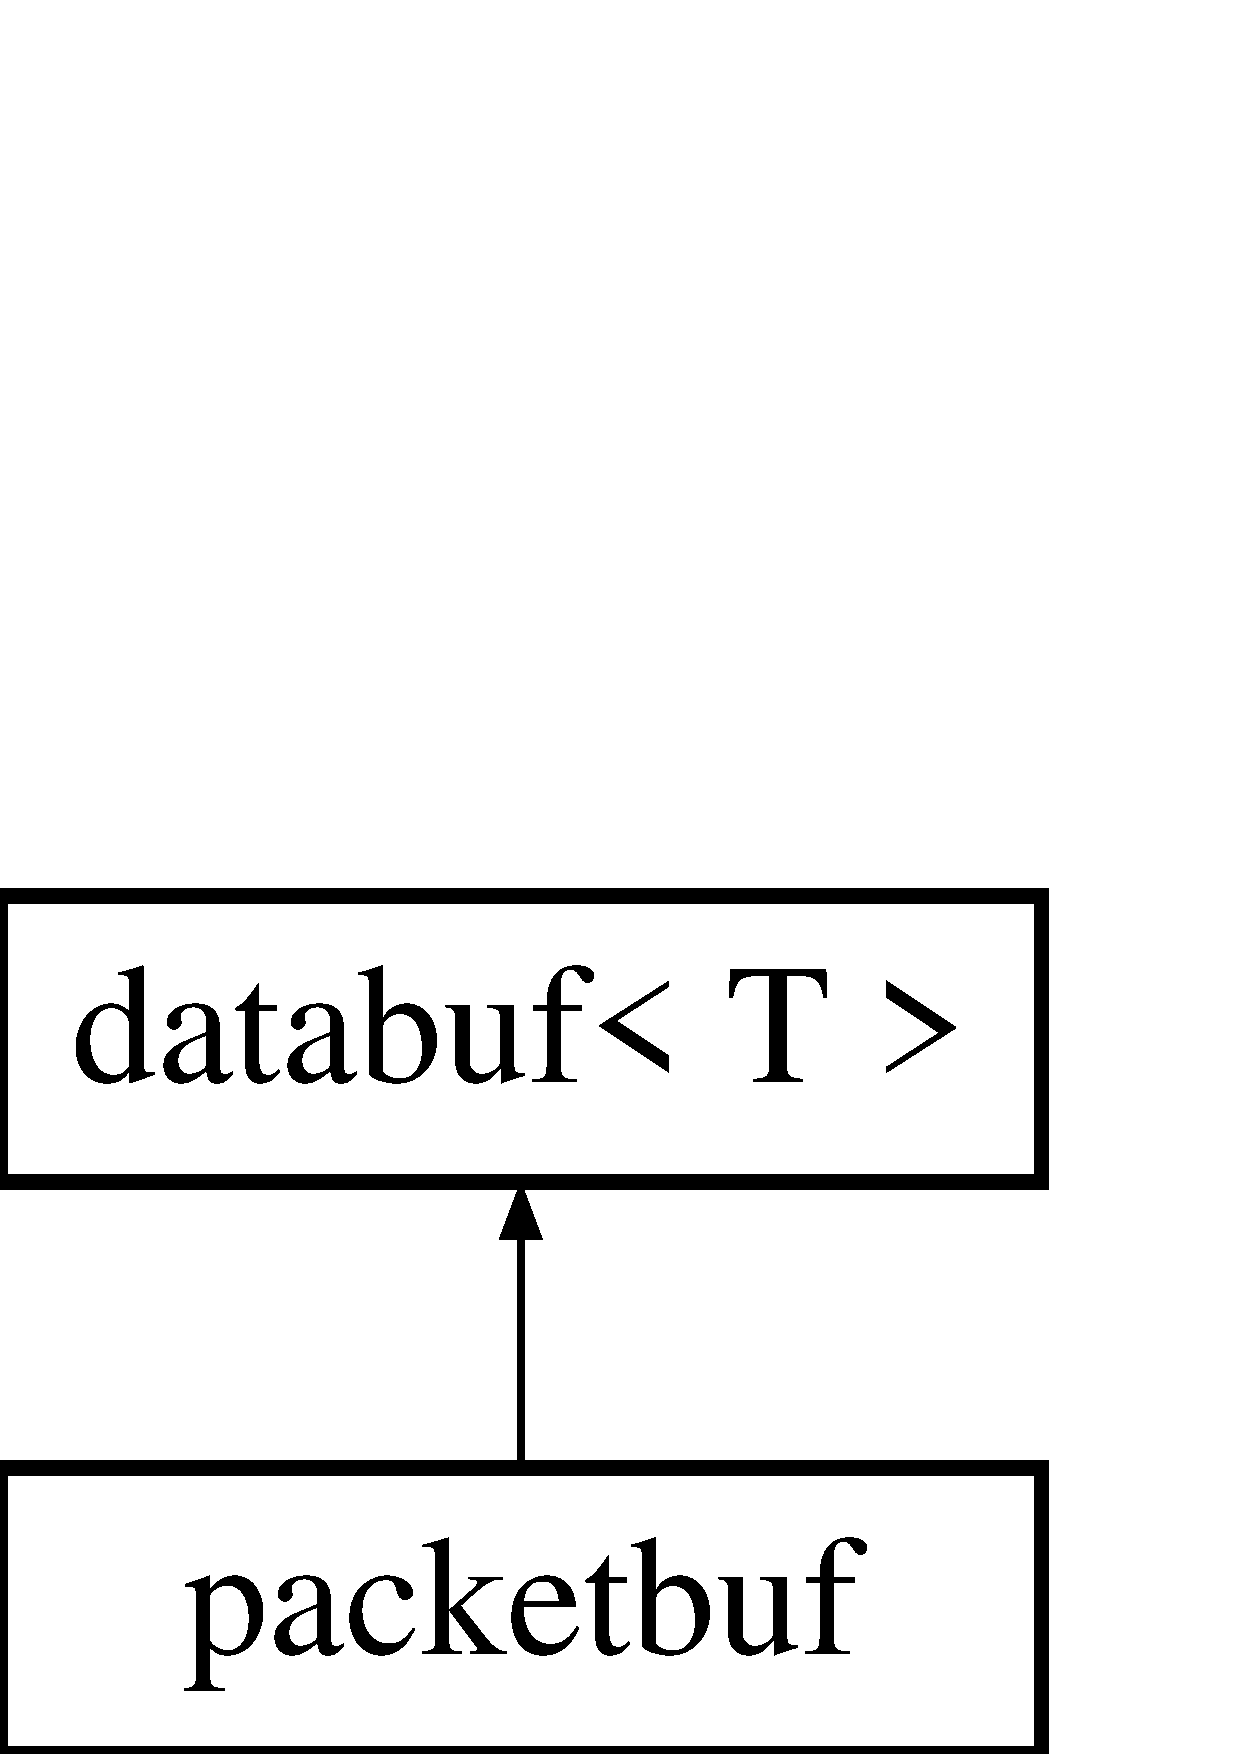
\includegraphics[height=2.000000cm]{structdatabuf}
\end{center}
\end{figure}
\subsection*{Public Types}
\begin{DoxyCompactItemize}
\item 
\mbox{\Hypertarget{structdatabuf_a9f408ad611db258c6fc64595f7174563}\label{structdatabuf_a9f408ad611db258c6fc64595f7174563}} 
enum \{ {\bfseries O\+V\+E\+R\+R\+E\+AD} = 1$<$$<$0, 
{\bfseries O\+V\+E\+R\+W\+R\+O\+TE} = 1$<$$<$1
 \}
\end{DoxyCompactItemize}
\subsection*{Public Member Functions}
\begin{DoxyCompactItemize}
\item 
\mbox{\Hypertarget{structdatabuf_af4e9590924e4b7d1c4a73a0d8060dfee}\label{structdatabuf_af4e9590924e4b7d1c4a73a0d8060dfee}} 
{\footnotesize template$<$class U $>$ }\\{\bfseries databuf} (T $\ast$buf, U maxlen)
\item 
\mbox{\Hypertarget{structdatabuf_ae8438cb4176e0ef2c7f84a6f891d0928}\label{structdatabuf_ae8438cb4176e0ef2c7f84a6f891d0928}} 
void {\bfseries reset} ()
\item 
\mbox{\Hypertarget{structdatabuf_a97129b48c69981fc8581dd16eabe6622}\label{structdatabuf_a97129b48c69981fc8581dd16eabe6622}} 
void {\bfseries reset} (T $\ast$buf\+\_\+, int maxlen\+\_\+)
\item 
\mbox{\Hypertarget{structdatabuf_aa7f496dc497379a8ceb61f1d359c4cfe}\label{structdatabuf_aa7f496dc497379a8ceb61f1d359c4cfe}} 
const T \& {\bfseries get} ()
\item 
\mbox{\Hypertarget{structdatabuf_a531caf46f8bf35bb2a16b4e7bc294b6c}\label{structdatabuf_a531caf46f8bf35bb2a16b4e7bc294b6c}} 
\hyperlink{structdatabuf}{databuf} {\bfseries subbuf} (int sz)
\item 
\mbox{\Hypertarget{structdatabuf_a62a0a7a3ec876a9a33d10c9e98cddf82}\label{structdatabuf_a62a0a7a3ec876a9a33d10c9e98cddf82}} 
T $\ast$ {\bfseries pad} (int numvals)
\item 
\mbox{\Hypertarget{structdatabuf_a4ddb1dbc1bcc6e5c589bb248060b2e24}\label{structdatabuf_a4ddb1dbc1bcc6e5c589bb248060b2e24}} 
void {\bfseries put} (const T \&val)
\item 
\mbox{\Hypertarget{structdatabuf_aa22fdfb9de579e0aa2a95b413f7aa9fe}\label{structdatabuf_aa22fdfb9de579e0aa2a95b413f7aa9fe}} 
void {\bfseries put} (const T $\ast$vals, int numvals)
\item 
\mbox{\Hypertarget{structdatabuf_ad1955ab60fbf7b6eb7a778c9361fe77d}\label{structdatabuf_ad1955ab60fbf7b6eb7a778c9361fe77d}} 
int {\bfseries get} (T $\ast$vals, int numvals)
\item 
\mbox{\Hypertarget{structdatabuf_ad5b5187b99d3dab4242ae6305b2d703c}\label{structdatabuf_ad5b5187b99d3dab4242ae6305b2d703c}} 
void {\bfseries offset} (int n)
\item 
\mbox{\Hypertarget{structdatabuf_aabe7049430ef398a4ae0d4dce7902277}\label{structdatabuf_aabe7049430ef398a4ae0d4dce7902277}} 
T $\ast$ {\bfseries getbuf} () const
\item 
\mbox{\Hypertarget{structdatabuf_ac462a5159900a306d67117cabbbf17db}\label{structdatabuf_ac462a5159900a306d67117cabbbf17db}} 
bool {\bfseries empty} () const
\item 
\mbox{\Hypertarget{structdatabuf_a49524245867f8f8b7a7e8d5a6c2e9afa}\label{structdatabuf_a49524245867f8f8b7a7e8d5a6c2e9afa}} 
int {\bfseries length} () const
\item 
\mbox{\Hypertarget{structdatabuf_a9e6bb0d4a4c7e47495c1b33d9856337e}\label{structdatabuf_a9e6bb0d4a4c7e47495c1b33d9856337e}} 
int {\bfseries remaining} () const
\item 
\mbox{\Hypertarget{structdatabuf_a7c8c5031dcedbf681924e5166ea190ae}\label{structdatabuf_a7c8c5031dcedbf681924e5166ea190ae}} 
bool {\bfseries overread} () const
\item 
\mbox{\Hypertarget{structdatabuf_af6060c72019fdeaf82ea0810091800b6}\label{structdatabuf_af6060c72019fdeaf82ea0810091800b6}} 
bool {\bfseries overwrote} () const
\item 
\mbox{\Hypertarget{structdatabuf_a058c8df40617db3950380737db05bc9a}\label{structdatabuf_a058c8df40617db3950380737db05bc9a}} 
bool {\bfseries check} (int n)
\item 
\mbox{\Hypertarget{structdatabuf_a9b2f3053e983a1a13f996d075a2307ac}\label{structdatabuf_a9b2f3053e983a1a13f996d075a2307ac}} 
void {\bfseries forceoverread} ()
\end{DoxyCompactItemize}
\subsection*{Public Attributes}
\begin{DoxyCompactItemize}
\item 
\mbox{\Hypertarget{structdatabuf_aef32e06b0075f5a381828441812c1b72}\label{structdatabuf_aef32e06b0075f5a381828441812c1b72}} 
T $\ast$ {\bfseries buf}
\item 
\mbox{\Hypertarget{structdatabuf_a2b4059e109b57415a9b3425364f6529c}\label{structdatabuf_a2b4059e109b57415a9b3425364f6529c}} 
int {\bfseries len}
\item 
\mbox{\Hypertarget{structdatabuf_ade4f8ac2ce53d313a1b1024eafcae9f2}\label{structdatabuf_ade4f8ac2ce53d313a1b1024eafcae9f2}} 
int {\bfseries maxlen}
\item 
\mbox{\Hypertarget{structdatabuf_a90dff9f73f4103c4ff0cc151de2c12b3}\label{structdatabuf_a90dff9f73f4103c4ff0cc151de2c12b3}} 
uchar {\bfseries flags}
\end{DoxyCompactItemize}


The documentation for this struct was generated from the following file\+:\begin{DoxyCompactItemize}
\item 
H\+:/\+Rival\+Engine/\+Rival\+\_\+\+Game\+\_\+\+Engine\+\_\+\+G\+I\+T/\+Rival3dengine/source/shared/tools.\+h\end{DoxyCompactItemize}

\hypertarget{struct_data_hold}{}\section{Data\+Hold Struct Reference}
\label{struct_data_hold}\index{Data\+Hold@{Data\+Hold}}
\subsection*{Public Member Functions}
\begin{DoxyCompactItemize}
\item 
\mbox{\Hypertarget{struct_data_hold_aab19e78f263134ddf49b032b035c4a8f}\label{struct_data_hold_aab19e78f263134ddf49b032b035c4a8f}} 
{\bfseries Data\+Hold} (uint ns\+ID, uint t\+ID, uint n\+ID)
\item 
\mbox{\Hypertarget{struct_data_hold_acf2518a53dc1f3eca61d8cb573540230}\label{struct_data_hold_acf2518a53dc1f3eca61d8cb573540230}} 
void {\bfseries print} ()
\item 
\mbox{\Hypertarget{struct_data_hold_aabf132bdb2fe1613da0c2e5732af07b6}\label{struct_data_hold_aabf132bdb2fe1613da0c2e5732af07b6}} 
void {\bfseries write} (\hyperlink{structstream}{stream} $\ast$f)
\item 
\mbox{\Hypertarget{struct_data_hold_acd46ba9f1539b30989c016d55fe7803a}\label{struct_data_hold_acd46ba9f1539b30989c016d55fe7803a}} 
int {\bfseries count} (uint start)
\end{DoxyCompactItemize}
\subsection*{Static Public Member Functions}
\begin{DoxyCompactItemize}
\item 
\mbox{\Hypertarget{struct_data_hold_a4f6f4b5e6880374ede633273d6c2b14e}\label{struct_data_hold_a4f6f4b5e6880374ede633273d6c2b14e}} 
static \hyperlink{struct_data_hold}{Data\+Hold} $\ast$ {\bfseries read} (\hyperlink{structstream}{stream} $\ast$f)
\end{DoxyCompactItemize}
\subsection*{Public Attributes}
\begin{DoxyCompactItemize}
\item 
\mbox{\Hypertarget{struct_data_hold_adc5aefe257c77de82fe36f3a020fd0f4}\label{struct_data_hold_adc5aefe257c77de82fe36f3a020fd0f4}} 
std\+::vector$<$ char $>$ {\bfseries data}
\item 
\mbox{\Hypertarget{struct_data_hold_ae70f2c9095266585b0be10739b50f581}\label{struct_data_hold_ae70f2c9095266585b0be10739b50f581}} 
uint {\bfseries children}
\item 
\mbox{\Hypertarget{struct_data_hold_a71d617c7ef82c971b937c14ee9010f54}\label{struct_data_hold_a71d617c7ef82c971b937c14ee9010f54}} 
uint {\bfseries namespace\+ID}
\item 
\mbox{\Hypertarget{struct_data_hold_ae0e671f123d5addeb9b59295f4f3d02e}\label{struct_data_hold_ae0e671f123d5addeb9b59295f4f3d02e}} 
uint {\bfseries name\+ID}
\item 
\mbox{\Hypertarget{struct_data_hold_af04a3e28f0cdc424cbdcd44547b7c230}\label{struct_data_hold_af04a3e28f0cdc424cbdcd44547b7c230}} 
uint {\bfseries type\+ID}
\item 
\mbox{\Hypertarget{struct_data_hold_a34243d77edd2fcbb68341906a150a667}\label{struct_data_hold_a34243d77edd2fcbb68341906a150a667}} 
\hyperlink{structvector}{vector}$<$ \hyperlink{struct_data_hold}{Data\+Hold} $\ast$ $>$ {\bfseries childs} = \hyperlink{structvector}{vector}$<$\hyperlink{struct_data_hold}{Data\+Hold} $\ast$$>$()
\end{DoxyCompactItemize}


The documentation for this struct was generated from the following file\+:\begin{DoxyCompactItemize}
\item 
H\+:/\+Rival\+Engine/\+Rival\+\_\+\+Game\+\_\+\+Engine\+\_\+\+G\+I\+T/\+Rival3dengine/source/shared/serializer.\+cpp\end{DoxyCompactItemize}

\hypertarget{struct_d_d_c_o_l_o_r_k_e_y}{}\section{D\+D\+C\+O\+L\+O\+R\+K\+EY Struct Reference}
\label{struct_d_d_c_o_l_o_r_k_e_y}\index{D\+D\+C\+O\+L\+O\+R\+K\+EY@{D\+D\+C\+O\+L\+O\+R\+K\+EY}}
\subsection*{Public Attributes}
\begin{DoxyCompactItemize}
\item 
\mbox{\Hypertarget{struct_d_d_c_o_l_o_r_k_e_y_ab66923eb20f38588a6214cf562f3de9d}\label{struct_d_d_c_o_l_o_r_k_e_y_ab66923eb20f38588a6214cf562f3de9d}} 
uint {\bfseries dw\+Color\+Space\+Low\+Value}
\item 
\mbox{\Hypertarget{struct_d_d_c_o_l_o_r_k_e_y_a19b1ff4a4d102b661372afbad864bb2a}\label{struct_d_d_c_o_l_o_r_k_e_y_a19b1ff4a4d102b661372afbad864bb2a}} 
uint {\bfseries dw\+Color\+Space\+High\+Value}
\end{DoxyCompactItemize}


The documentation for this struct was generated from the following file\+:\begin{DoxyCompactItemize}
\item 
H\+:/\+Rival\+Engine/\+Rival\+\_\+\+Game\+\_\+\+Engine\+\_\+\+G\+I\+T/\+Rival3dengine/source/engine/texture.\+cpp\end{DoxyCompactItemize}

\hypertarget{struct_d_d_p_i_x_e_l_f_o_r_m_a_t}{}\section{D\+D\+P\+I\+X\+E\+L\+F\+O\+R\+M\+AT Struct Reference}
\label{struct_d_d_p_i_x_e_l_f_o_r_m_a_t}\index{D\+D\+P\+I\+X\+E\+L\+F\+O\+R\+M\+AT@{D\+D\+P\+I\+X\+E\+L\+F\+O\+R\+M\+AT}}
\subsection*{Public Attributes}
\begin{DoxyCompactItemize}
\item 
\mbox{\Hypertarget{struct_d_d_p_i_x_e_l_f_o_r_m_a_t_ad57e694d40d45ceed426de894dbfe792}\label{struct_d_d_p_i_x_e_l_f_o_r_m_a_t_ad57e694d40d45ceed426de894dbfe792}} 
uint {\bfseries dw\+Size}
\item 
\mbox{\Hypertarget{struct_d_d_p_i_x_e_l_f_o_r_m_a_t_afcd627a47c9b2fb99a2549de9568f325}\label{struct_d_d_p_i_x_e_l_f_o_r_m_a_t_afcd627a47c9b2fb99a2549de9568f325}} 
uint {\bfseries dw\+Flags}
\item 
\mbox{\Hypertarget{struct_d_d_p_i_x_e_l_f_o_r_m_a_t_ad332a4a4e3972e554afbb349d4d2776c}\label{struct_d_d_p_i_x_e_l_f_o_r_m_a_t_ad332a4a4e3972e554afbb349d4d2776c}} 
uint {\bfseries dw\+Four\+CC}
\item 
\mbox{\Hypertarget{struct_d_d_p_i_x_e_l_f_o_r_m_a_t_aa044ef9c87f30487cee120add36bbabd}\label{struct_d_d_p_i_x_e_l_f_o_r_m_a_t_aa044ef9c87f30487cee120add36bbabd}} 
\begin{tabbing}
xx\=xx\=xx\=xx\=xx\=xx\=xx\=xx\=xx\=\kill
union \{\\
\>uint {\bfseries dwRGBBitCount}\\
\>uint {\bfseries dwYUVBitCount}\\
\>uint {\bfseries dwZBufferBitDepth}\\
\>uint {\bfseries dwAlphaBitDepth}\\
\>uint {\bfseries dwLuminanceBitCount}\\
\>uint {\bfseries dwBumpBitCount}\\
\>uint {\bfseries dwPrivateFormatBitCount}\\
\}; \\

\end{tabbing}\item 
\mbox{\Hypertarget{struct_d_d_p_i_x_e_l_f_o_r_m_a_t_a19d8edbb996bd71622a0f5acd919dd2c}\label{struct_d_d_p_i_x_e_l_f_o_r_m_a_t_a19d8edbb996bd71622a0f5acd919dd2c}} 
\begin{tabbing}
xx\=xx\=xx\=xx\=xx\=xx\=xx\=xx\=xx\=\kill
union \{\\
\>uint {\bfseries dwRBitMask}\\
\>uint {\bfseries dwYBitMask}\\
\>uint {\bfseries dwStencilBitDepth}\\
\>uint {\bfseries dwLuminanceBitMask}\\
\>uint {\bfseries dwBumpDuBitMask}\\
\>uint {\bfseries dwOperations}\\
\}; \\

\end{tabbing}\item 
\mbox{\Hypertarget{struct_d_d_p_i_x_e_l_f_o_r_m_a_t_acd95bd5d5b6108af6e3f97b0cc45cf5a}\label{struct_d_d_p_i_x_e_l_f_o_r_m_a_t_acd95bd5d5b6108af6e3f97b0cc45cf5a}} 
\begin{tabbing}
xx\=xx\=xx\=xx\=xx\=xx\=xx\=xx\=xx\=\kill
union \{\\
\>uint {\bfseries dwGBitMask}\\
\>uint {\bfseries dwUBitMask}\\
\>uint {\bfseries dwZBitMask}\\
\>uint {\bfseries dwBumpDvBitMask}\\
\>struct \{\\
\>\>ushort {\bfseries wFlipMSTypes}\\
\>\>ushort {\bfseries wBltMSTypes}\\
\>\} {\bfseries MultiSampleCaps}\\
\}; \\

\end{tabbing}\item 
\mbox{\Hypertarget{struct_d_d_p_i_x_e_l_f_o_r_m_a_t_a71ca6637b13f56ecadb77528f9c0b472}\label{struct_d_d_p_i_x_e_l_f_o_r_m_a_t_a71ca6637b13f56ecadb77528f9c0b472}} 
\begin{tabbing}
xx\=xx\=xx\=xx\=xx\=xx\=xx\=xx\=xx\=\kill
union \{\\
\>uint {\bfseries dwBBitMask}\\
\>uint {\bfseries dwVBitMask}\\
\>uint {\bfseries dwStencilBitMask}\\
\>uint {\bfseries dwBumpLuminanceBitMask}\\
\}; \\

\end{tabbing}\item 
\mbox{\Hypertarget{struct_d_d_p_i_x_e_l_f_o_r_m_a_t_a701f48da25ed22170c8d89faa16f8637}\label{struct_d_d_p_i_x_e_l_f_o_r_m_a_t_a701f48da25ed22170c8d89faa16f8637}} 
\begin{tabbing}
xx\=xx\=xx\=xx\=xx\=xx\=xx\=xx\=xx\=\kill
union \{\\
\>uint {\bfseries dwRGBAlphaBitMask}\\
\>uint {\bfseries dwYUVAlphaBitMask}\\
\>uint {\bfseries dwLuminanceAlphaBitMask}\\
\>uint {\bfseries dwRGBZBitMask}\\
\>uint {\bfseries dwYUVZBitMask}\\
\}; \\

\end{tabbing}\end{DoxyCompactItemize}


The documentation for this struct was generated from the following file\+:\begin{DoxyCompactItemize}
\item 
H\+:/\+Rival\+Engine/\+Rival\+\_\+\+Game\+\_\+\+Engine\+\_\+\+G\+I\+T/\+Rival3dengine/source/engine/texture.\+cpp\end{DoxyCompactItemize}

\hypertarget{struct_d_d_s_c_a_p_s2}{}\section{D\+D\+S\+C\+A\+P\+S2 Struct Reference}
\label{struct_d_d_s_c_a_p_s2}\index{D\+D\+S\+C\+A\+P\+S2@{D\+D\+S\+C\+A\+P\+S2}}
\subsection*{Public Attributes}
\begin{DoxyCompactItemize}
\item 
\mbox{\Hypertarget{struct_d_d_s_c_a_p_s2_aeeaa6e011753f9456d765e31412efc1b}\label{struct_d_d_s_c_a_p_s2_aeeaa6e011753f9456d765e31412efc1b}} 
uint {\bfseries dw\+Caps}
\item 
\mbox{\Hypertarget{struct_d_d_s_c_a_p_s2_afe77b601d123fb9584011c8b9f05050b}\label{struct_d_d_s_c_a_p_s2_afe77b601d123fb9584011c8b9f05050b}} 
uint {\bfseries dw\+Caps2}
\item 
\mbox{\Hypertarget{struct_d_d_s_c_a_p_s2_a0753215c432c8c49ffff942388f9b877}\label{struct_d_d_s_c_a_p_s2_a0753215c432c8c49ffff942388f9b877}} 
uint {\bfseries dw\+Caps3}
\item 
\mbox{\Hypertarget{struct_d_d_s_c_a_p_s2_a7068a2bec849d63e86fc4184185afaf2}\label{struct_d_d_s_c_a_p_s2_a7068a2bec849d63e86fc4184185afaf2}} 
uint {\bfseries dw\+Caps4}
\end{DoxyCompactItemize}


The documentation for this struct was generated from the following file\+:\begin{DoxyCompactItemize}
\item 
H\+:/\+Rival\+Engine/\+Rival\+\_\+\+Game\+\_\+\+Engine\+\_\+\+G\+I\+T/\+Rival3dengine/source/engine/texture.\+cpp\end{DoxyCompactItemize}

\hypertarget{struct_d_d_s_u_r_f_a_c_e_d_e_s_c2}{}\section{D\+D\+S\+U\+R\+F\+A\+C\+E\+D\+E\+S\+C2 Struct Reference}
\label{struct_d_d_s_u_r_f_a_c_e_d_e_s_c2}\index{D\+D\+S\+U\+R\+F\+A\+C\+E\+D\+E\+S\+C2@{D\+D\+S\+U\+R\+F\+A\+C\+E\+D\+E\+S\+C2}}
\subsection*{Public Attributes}
\begin{DoxyCompactItemize}
\item 
\mbox{\Hypertarget{struct_d_d_s_u_r_f_a_c_e_d_e_s_c2_aa86f74b7f3b67f51928470b717663eed}\label{struct_d_d_s_u_r_f_a_c_e_d_e_s_c2_aa86f74b7f3b67f51928470b717663eed}} 
uint {\bfseries dw\+Size}
\item 
\mbox{\Hypertarget{struct_d_d_s_u_r_f_a_c_e_d_e_s_c2_a01003dd668221026a147075177e57607}\label{struct_d_d_s_u_r_f_a_c_e_d_e_s_c2_a01003dd668221026a147075177e57607}} 
uint {\bfseries dw\+Flags}
\item 
\mbox{\Hypertarget{struct_d_d_s_u_r_f_a_c_e_d_e_s_c2_a2fa974c393dceaef70025b65b69da0c4}\label{struct_d_d_s_u_r_f_a_c_e_d_e_s_c2_a2fa974c393dceaef70025b65b69da0c4}} 
uint {\bfseries dw\+Height}
\item 
\mbox{\Hypertarget{struct_d_d_s_u_r_f_a_c_e_d_e_s_c2_a83b7976f8c3c5710d2bb005c2e64f688}\label{struct_d_d_s_u_r_f_a_c_e_d_e_s_c2_a83b7976f8c3c5710d2bb005c2e64f688}} 
uint {\bfseries dw\+Width}
\item 
\mbox{\Hypertarget{struct_d_d_s_u_r_f_a_c_e_d_e_s_c2_a3d18871195d51e6f54bc54890d711146}\label{struct_d_d_s_u_r_f_a_c_e_d_e_s_c2_a3d18871195d51e6f54bc54890d711146}} 
\begin{tabbing}
xx\=xx\=xx\=xx\=xx\=xx\=xx\=xx\=xx\=\kill
union \{\\
\>int {\bfseries lPitch}\\
\>uint {\bfseries dwLinearSize}\\
\}; \\

\end{tabbing}\item 
\mbox{\Hypertarget{struct_d_d_s_u_r_f_a_c_e_d_e_s_c2_a9e79c97510cac5ef0353f24de1821312}\label{struct_d_d_s_u_r_f_a_c_e_d_e_s_c2_a9e79c97510cac5ef0353f24de1821312}} 
uint {\bfseries dw\+Back\+Buffer\+Count}
\item 
\mbox{\Hypertarget{struct_d_d_s_u_r_f_a_c_e_d_e_s_c2_a6164de9a3e358483c26397e02a500c06}\label{struct_d_d_s_u_r_f_a_c_e_d_e_s_c2_a6164de9a3e358483c26397e02a500c06}} 
\begin{tabbing}
xx\=xx\=xx\=xx\=xx\=xx\=xx\=xx\=xx\=\kill
union \{\\
\>uint {\bfseries dwMipMapCount}\\
\>uint {\bfseries dwRefreshRate}\\
\>uint {\bfseries dwSrcVBHandle}\\
\}; \\

\end{tabbing}\item 
\mbox{\Hypertarget{struct_d_d_s_u_r_f_a_c_e_d_e_s_c2_ad6a8c0b0ea9f7756797a75142c96cd42}\label{struct_d_d_s_u_r_f_a_c_e_d_e_s_c2_ad6a8c0b0ea9f7756797a75142c96cd42}} 
uint {\bfseries dw\+Alpha\+Bit\+Depth}
\item 
\mbox{\Hypertarget{struct_d_d_s_u_r_f_a_c_e_d_e_s_c2_a980b41e3171b7623cbfffe6dfddc5906}\label{struct_d_d_s_u_r_f_a_c_e_d_e_s_c2_a980b41e3171b7623cbfffe6dfddc5906}} 
uint {\bfseries dw\+Reserved}
\item 
\mbox{\Hypertarget{struct_d_d_s_u_r_f_a_c_e_d_e_s_c2_a283d284a2ad3f6e7eb9ca0d4cef4c690}\label{struct_d_d_s_u_r_f_a_c_e_d_e_s_c2_a283d284a2ad3f6e7eb9ca0d4cef4c690}} 
uint {\bfseries lp\+Surface}
\item 
\mbox{\Hypertarget{struct_d_d_s_u_r_f_a_c_e_d_e_s_c2_ac7b28d880e45e9c7a077494f8c995d5f}\label{struct_d_d_s_u_r_f_a_c_e_d_e_s_c2_ac7b28d880e45e9c7a077494f8c995d5f}} 
\begin{tabbing}
xx\=xx\=xx\=xx\=xx\=xx\=xx\=xx\=xx\=\kill
union \{\\
\>\hyperlink{struct_d_d_c_o_l_o_r_k_e_y}{DDCOLORKEY} {\bfseries ddckCKDestOverlay}\\
\>uint {\bfseries dwEmptyFaceColor}\\
\}; \\

\end{tabbing}\item 
\mbox{\Hypertarget{struct_d_d_s_u_r_f_a_c_e_d_e_s_c2_aa5c27e8a198a03a72a543263a034ac11}\label{struct_d_d_s_u_r_f_a_c_e_d_e_s_c2_aa5c27e8a198a03a72a543263a034ac11}} 
\hyperlink{struct_d_d_c_o_l_o_r_k_e_y}{D\+D\+C\+O\+L\+O\+R\+K\+EY} {\bfseries ddck\+C\+K\+Dest\+Blt}
\item 
\mbox{\Hypertarget{struct_d_d_s_u_r_f_a_c_e_d_e_s_c2_af22c85d5804581fca26e00c402145ac6}\label{struct_d_d_s_u_r_f_a_c_e_d_e_s_c2_af22c85d5804581fca26e00c402145ac6}} 
\hyperlink{struct_d_d_c_o_l_o_r_k_e_y}{D\+D\+C\+O\+L\+O\+R\+K\+EY} {\bfseries ddck\+C\+K\+Src\+Overlay}
\item 
\mbox{\Hypertarget{struct_d_d_s_u_r_f_a_c_e_d_e_s_c2_ab867f780f3b125326eb4a38522d10e58}\label{struct_d_d_s_u_r_f_a_c_e_d_e_s_c2_ab867f780f3b125326eb4a38522d10e58}} 
\hyperlink{struct_d_d_c_o_l_o_r_k_e_y}{D\+D\+C\+O\+L\+O\+R\+K\+EY} {\bfseries ddck\+C\+K\+Src\+Blt}
\item 
\mbox{\Hypertarget{struct_d_d_s_u_r_f_a_c_e_d_e_s_c2_a138709477e2c5f9a3cd101dd8d208ca8}\label{struct_d_d_s_u_r_f_a_c_e_d_e_s_c2_a138709477e2c5f9a3cd101dd8d208ca8}} 
\begin{tabbing}
xx\=xx\=xx\=xx\=xx\=xx\=xx\=xx\=xx\=\kill
union \{\\
\>\hyperlink{struct_d_d_p_i_x_e_l_f_o_r_m_a_t}{DDPIXELFORMAT} {\bfseries ddpfPixelFormat}\\
\>uint {\bfseries dwFVF}\\
\}; \\

\end{tabbing}\item 
\mbox{\Hypertarget{struct_d_d_s_u_r_f_a_c_e_d_e_s_c2_add6306ce126a7a97679376651e7c3587}\label{struct_d_d_s_u_r_f_a_c_e_d_e_s_c2_add6306ce126a7a97679376651e7c3587}} 
\hyperlink{struct_d_d_s_c_a_p_s2}{D\+D\+S\+C\+A\+P\+S2} {\bfseries dds\+Caps}
\item 
\mbox{\Hypertarget{struct_d_d_s_u_r_f_a_c_e_d_e_s_c2_ae1b360c27dccdc46d38b2b124dec2f09}\label{struct_d_d_s_u_r_f_a_c_e_d_e_s_c2_ae1b360c27dccdc46d38b2b124dec2f09}} 
uint {\bfseries dw\+Texture\+Stage}
\end{DoxyCompactItemize}


The documentation for this struct was generated from the following file\+:\begin{DoxyCompactItemize}
\item 
H\+:/\+Rival\+Engine/\+Rival\+\_\+\+Game\+\_\+\+Engine\+\_\+\+G\+I\+T/\+Rival3dengine/source/engine/texture.\+cpp\end{DoxyCompactItemize}

\hypertarget{structdecalbatch}{}\section{decalbatch Struct Reference}
\label{structdecalbatch}\index{decalbatch@{decalbatch}}
\subsection*{Public Member Functions}
\begin{DoxyCompactItemize}
\item 
\mbox{\Hypertarget{structdecalbatch_ae9dc4884b83948f7675f69b2dcf7a29e}\label{structdecalbatch_ae9dc4884b83948f7675f69b2dcf7a29e}} 
{\bfseries decalbatch} (const \hyperlink{structelementset}{elementset} \&es, int offset, \hyperlink{structvtxarray}{vtxarray} $\ast$va)
\item 
\mbox{\Hypertarget{structdecalbatch_aa859444a701df954399ddc0f172fa830}\label{structdecalbatch_aa859444a701df954399ddc0f172fa830}} 
int {\bfseries compare} (const \hyperlink{structdecalbatch}{decalbatch} \&b) const
\end{DoxyCompactItemize}
\subsection*{Public Attributes}
\begin{DoxyCompactItemize}
\item 
\mbox{\Hypertarget{structdecalbatch_aace50ea9908f4c82f1d732a640012965}\label{structdecalbatch_aace50ea9908f4c82f1d732a640012965}} 
const \hyperlink{structelementset}{elementset} \& {\bfseries es}
\item 
\mbox{\Hypertarget{structdecalbatch_af0ecebffb6181db506828de930e0471e}\label{structdecalbatch_af0ecebffb6181db506828de930e0471e}} 
\hyperlink{struct_decal_slot}{Decal\+Slot} \& {\bfseries slot}
\item 
\mbox{\Hypertarget{structdecalbatch_a855f47422bdbaf7b903d7d5659f180ee}\label{structdecalbatch_a855f47422bdbaf7b903d7d5659f180ee}} 
int {\bfseries offset}
\item 
\mbox{\Hypertarget{structdecalbatch_ab7b0be0021cfc41293c89e5b1894375c}\label{structdecalbatch_ab7b0be0021cfc41293c89e5b1894375c}} 
\hyperlink{structvtxarray}{vtxarray} $\ast$ {\bfseries va}
\item 
\mbox{\Hypertarget{structdecalbatch_aeee5aa6e9b104269e95b0aa98e2718e3}\label{structdecalbatch_aeee5aa6e9b104269e95b0aa98e2718e3}} 
int {\bfseries next}
\item 
\mbox{\Hypertarget{structdecalbatch_aa436ce54497590f95d034dff6058cc91}\label{structdecalbatch_aa436ce54497590f95d034dff6058cc91}} 
int {\bfseries batch}
\end{DoxyCompactItemize}


The documentation for this struct was generated from the following file\+:\begin{DoxyCompactItemize}
\item 
H\+:/\+Rival\+Engine/\+Rival\+\_\+\+Game\+\_\+\+Engine\+\_\+\+G\+I\+T/\+Rival3dengine/source/engine/renderva.\+cpp\end{DoxyCompactItemize}

\hypertarget{structdecalkey}{}\section{decalkey Struct Reference}
\label{structdecalkey}\index{decalkey@{decalkey}}
\subsection*{Public Member Functions}
\begin{DoxyCompactItemize}
\item 
\mbox{\Hypertarget{structdecalkey_a7353aef9e5f7457567ea34b9473799af}\label{structdecalkey_a7353aef9e5f7457567ea34b9473799af}} 
{\bfseries decalkey} (ushort tex, ushort \hyperlink{structenvmap}{envmap}=E\+M\+I\+D\+\_\+\+N\+O\+NE, ushort reuse=0)
\item 
\mbox{\Hypertarget{structdecalkey_a202dc581b104c5239d2e9ed8c89f4035}\label{structdecalkey_a202dc581b104c5239d2e9ed8c89f4035}} 
bool {\bfseries operator==} (const \hyperlink{structdecalkey}{decalkey} \&o) const
\end{DoxyCompactItemize}
\subsection*{Static Public Member Functions}
\begin{DoxyCompactItemize}
\item 
\mbox{\Hypertarget{structdecalkey_a43d94ec2066d77ccf8336befce9a389c}\label{structdecalkey_a43d94ec2066d77ccf8336befce9a389c}} 
static bool {\bfseries sort} (const \hyperlink{structdecalkey}{decalkey} \&x, const \hyperlink{structdecalkey}{decalkey} \&y)
\end{DoxyCompactItemize}
\subsection*{Public Attributes}
\begin{DoxyCompactItemize}
\item 
\mbox{\Hypertarget{structdecalkey_ae8fc3afbb436de2ff981bbd2c96a1fac}\label{structdecalkey_ae8fc3afbb436de2ff981bbd2c96a1fac}} 
ushort {\bfseries tex}
\item 
\mbox{\Hypertarget{structdecalkey_a70fc4be3c3707a7f0adddbc6a3ec3010}\label{structdecalkey_a70fc4be3c3707a7f0adddbc6a3ec3010}} 
ushort {\bfseries envmap}
\item 
\mbox{\Hypertarget{structdecalkey_afb306180c6e47a96ac4613370c7b8dbc}\label{structdecalkey_afb306180c6e47a96ac4613370c7b8dbc}} 
ushort {\bfseries reuse}
\end{DoxyCompactItemize}


The documentation for this struct was generated from the following file\+:\begin{DoxyCompactItemize}
\item 
H\+:/\+Rival\+Engine/\+Rival\+\_\+\+Game\+\_\+\+Engine\+\_\+\+G\+I\+T/\+Rival3dengine/source/engine/octarender.\+cpp\end{DoxyCompactItemize}

\hypertarget{structdecalrenderer}{}\section{decalrenderer Struct Reference}
\label{structdecalrenderer}\index{decalrenderer@{decalrenderer}}
\subsection*{Public Attributes}
\begin{DoxyCompactItemize}
\item 
\mbox{\Hypertarget{structdecalrenderer_adfaaeb04fc305f58a585b0f1fb242f68}\label{structdecalrenderer_adfaaeb04fc305f58a585b0f1fb242f68}} 
G\+Luint {\bfseries vbuf}
\item 
\mbox{\Hypertarget{structdecalrenderer_a284e483a01a01567f2719ff043cf3e6c}\label{structdecalrenderer_a284e483a01a01567f2719ff043cf3e6c}} 
\hyperlink{structvec}{vec} {\bfseries colorscale}
\item 
\mbox{\Hypertarget{structdecalrenderer_a5819a8e64587a5f7e69906d301a784a1}\label{structdecalrenderer_a5819a8e64587a5f7e69906d301a784a1}} 
int {\bfseries globals}
\item 
\mbox{\Hypertarget{structdecalrenderer_ae4d3482f730a9e82493fa62ffe9009a7}\label{structdecalrenderer_ae4d3482f730a9e82493fa62ffe9009a7}} 
int {\bfseries tmu}
\item 
\mbox{\Hypertarget{structdecalrenderer_add575d0e2fc3c8f24e9b25848496c3a2}\label{structdecalrenderer_add575d0e2fc3c8f24e9b25848496c3a2}} 
G\+Luint {\bfseries textures} \mbox{[}7\mbox{]}
\item 
\mbox{\Hypertarget{structdecalrenderer_a58d234edeccb4c16b0c8de79ed955d37}\label{structdecalrenderer_a58d234edeccb4c16b0c8de79ed955d37}} 
\hyperlink{struct_decal_slot}{Decal\+Slot} $\ast$ {\bfseries slot}
\end{DoxyCompactItemize}


The documentation for this struct was generated from the following file\+:\begin{DoxyCompactItemize}
\item 
H\+:/\+Rival\+Engine/\+Rival\+\_\+\+Game\+\_\+\+Engine\+\_\+\+G\+I\+T/\+Rival3dengine/source/engine/renderva.\+cpp\end{DoxyCompactItemize}

\hypertarget{struct_decal_slot}{}\section{Decal\+Slot Struct Reference}
\label{struct_decal_slot}\index{Decal\+Slot@{Decal\+Slot}}
Inheritance diagram for Decal\+Slot\+:\begin{figure}[H]
\begin{center}
\leavevmode
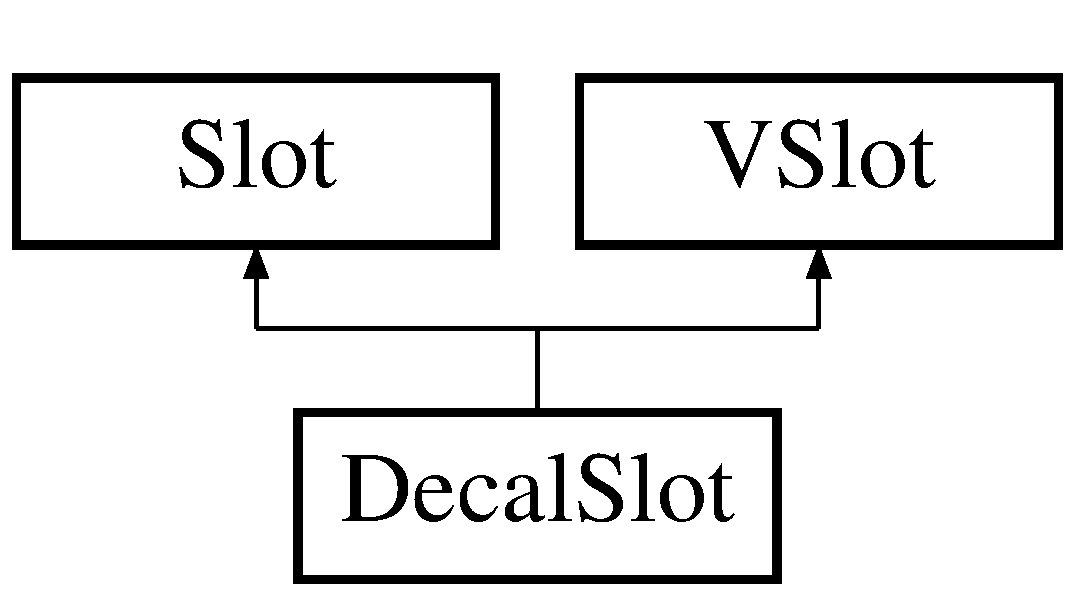
\includegraphics[height=2.000000cm]{struct_decal_slot}
\end{center}
\end{figure}
\subsection*{Public Member Functions}
\begin{DoxyCompactItemize}
\item 
\mbox{\Hypertarget{struct_decal_slot_a4f98aeb399d93efdec0d893392d8e63a}\label{struct_decal_slot_a4f98aeb399d93efdec0d893392d8e63a}} 
{\bfseries Decal\+Slot} (int index=-\/1)
\item 
\mbox{\Hypertarget{struct_decal_slot_abc8bf0b184e24ece3de462535ad231be}\label{struct_decal_slot_abc8bf0b184e24ece3de462535ad231be}} 
int {\bfseries type} () const
\item 
\mbox{\Hypertarget{struct_decal_slot_a2ce63e7f3051d55cdbf22ac8a3446d40}\label{struct_decal_slot_a2ce63e7f3051d55cdbf22ac8a3446d40}} 
const char $\ast$ {\bfseries name} () const
\item 
\mbox{\Hypertarget{struct_decal_slot_a11e475fa849bf5d8924ae5c72854dde5}\label{struct_decal_slot_a11e475fa849bf5d8924ae5c72854dde5}} 
const char $\ast$ {\bfseries texturedir} () const
\item 
\mbox{\Hypertarget{struct_decal_slot_a5d8d7d95178c1b97d4d2ca5279903f3b}\label{struct_decal_slot_a5d8d7d95178c1b97d4d2ca5279903f3b}} 
\hyperlink{struct_v_slot}{V\+Slot} \& {\bfseries emptyvslot} ()
\item 
\mbox{\Hypertarget{struct_decal_slot_a3c54bf7eb96a111234bccf6cfe2fb9c7}\label{struct_decal_slot_a3c54bf7eb96a111234bccf6cfe2fb9c7}} 
int {\bfseries cancombine} (int type) const
\item 
\mbox{\Hypertarget{struct_decal_slot_ac3be8a44ef390b993b41c565e3d893d5}\label{struct_decal_slot_ac3be8a44ef390b993b41c565e3d893d5}} 
void {\bfseries reset} ()
\item 
\mbox{\Hypertarget{struct_decal_slot_a89938de20425aa8768096539d872c7ec}\label{struct_decal_slot_a89938de20425aa8768096539d872c7ec}} 
void {\bfseries cleanup} ()
\end{DoxyCompactItemize}
\subsection*{Public Attributes}
\begin{DoxyCompactItemize}
\item 
\mbox{\Hypertarget{struct_decal_slot_a606e42405d3bbdd391d9eca85a0342b4}\label{struct_decal_slot_a606e42405d3bbdd391d9eca85a0342b4}} 
float {\bfseries depth}
\item 
\mbox{\Hypertarget{struct_decal_slot_aa7a4c1cabc3861339f0064bc820ad6c6}\label{struct_decal_slot_aa7a4c1cabc3861339f0064bc820ad6c6}} 
float {\bfseries fade}
\end{DoxyCompactItemize}
\subsection*{Additional Inherited Members}


The documentation for this struct was generated from the following files\+:\begin{DoxyCompactItemize}
\item 
H\+:/\+Rival\+Engine/\+Rival\+\_\+\+Game\+\_\+\+Engine\+\_\+\+G\+I\+T/\+Rival3dengine/source/engine/texture.\+h\item 
H\+:/\+Rival\+Engine/\+Rival\+\_\+\+Game\+\_\+\+Engine\+\_\+\+G\+I\+T/\+Rival3dengine/source/engine/texture.\+cpp\end{DoxyCompactItemize}

\hypertarget{structabc_1_1def}{}\section{abc\+:\+:def Struct Reference}
\label{structabc_1_1def}\index{abc\+::def@{abc\+::def}}
\subsection*{Public Attributes}
\begin{DoxyCompactItemize}
\item 
\mbox{\Hypertarget{structabc_1_1def_af7d08b31440cd001d29aa8f10515755c}\label{structabc_1_1def_af7d08b31440cd001d29aa8f10515755c}} 
char $\ast$ {\bfseries coolthing}
\item 
\mbox{\Hypertarget{structabc_1_1def_a6c1105a3e97805c51925b5aa85665808}\label{structabc_1_1def_a6c1105a3e97805c51925b5aa85665808}} 
uint {\bfseries index}
\end{DoxyCompactItemize}


The documentation for this struct was generated from the following file\+:\begin{DoxyCompactItemize}
\item 
H\+:/\+Rival\+Engine/\+Rival\+\_\+\+Game\+\_\+\+Engine\+\_\+\+G\+I\+T/\+Rival3dengine/source/engine/world.\+h\end{DoxyCompactItemize}

\hypertarget{structdefvar}{}\section{defvar Struct Reference}
\label{structdefvar}\index{defvar@{defvar}}
Inheritance diagram for defvar\+:\begin{figure}[H]
\begin{center}
\leavevmode
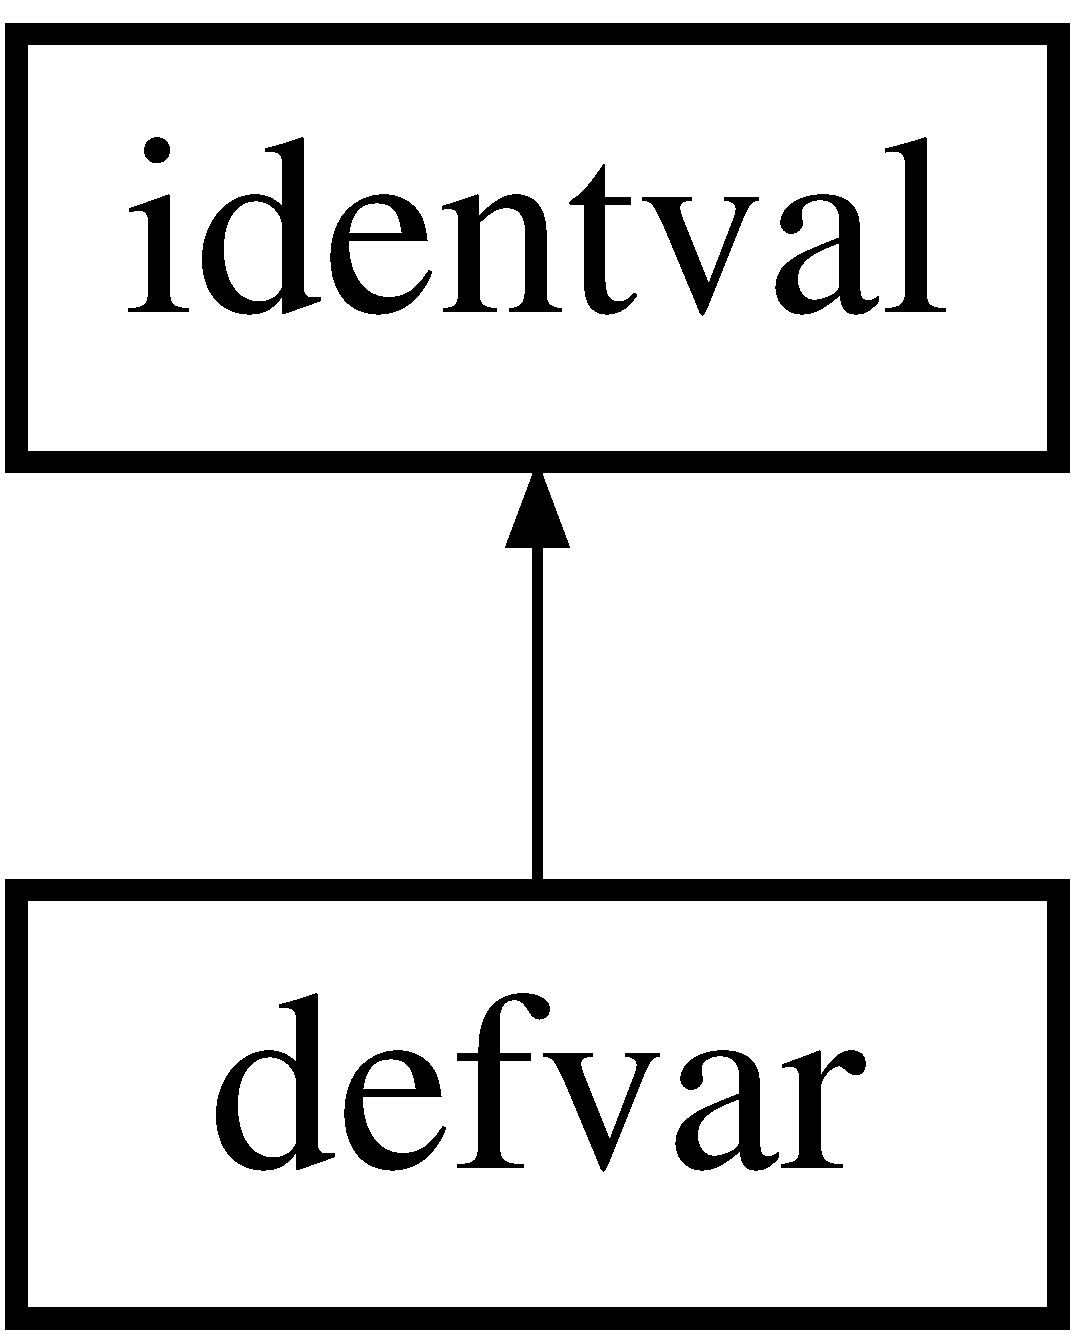
\includegraphics[height=2.000000cm]{structdefvar}
\end{center}
\end{figure}
\subsection*{Static Public Member Functions}
\begin{DoxyCompactItemize}
\item 
\mbox{\Hypertarget{structdefvar_ae876bdc4c67af25508a914d3230d93cd}\label{structdefvar_ae876bdc4c67af25508a914d3230d93cd}} 
static void {\bfseries changed} (\hyperlink{structident}{ident} $\ast$id)
\end{DoxyCompactItemize}
\subsection*{Public Attributes}
\begin{DoxyCompactItemize}
\item 
\mbox{\Hypertarget{structdefvar_aedc852f6371ffd13af82b7e045cc7e33}\label{structdefvar_aedc852f6371ffd13af82b7e045cc7e33}} 
char $\ast$ {\bfseries name}
\item 
\mbox{\Hypertarget{structdefvar_a46940060736bcc3cd2a74b24d2925cf0}\label{structdefvar_a46940060736bcc3cd2a74b24d2925cf0}} 
uint $\ast$ {\bfseries onchange}
\end{DoxyCompactItemize}


The documentation for this struct was generated from the following file\+:\begin{DoxyCompactItemize}
\item 
H\+:/\+Rival\+Engine/\+Rival\+\_\+\+Game\+\_\+\+Engine\+\_\+\+G\+I\+T/\+Rival3dengine/source/engine/command.\+cpp\end{DoxyCompactItemize}

\hypertarget{structserver_1_1demofile}{}\section{server\+:\+:demofile Struct Reference}
\label{structserver_1_1demofile}\index{server\+::demofile@{server\+::demofile}}
\subsection*{Public Attributes}
\begin{DoxyCompactItemize}
\item 
\mbox{\Hypertarget{structserver_1_1demofile_aeb45d37141ea1a970fcdadb4f09781ae}\label{structserver_1_1demofile_aeb45d37141ea1a970fcdadb4f09781ae}} 
cubestr {\bfseries info}
\item 
\mbox{\Hypertarget{structserver_1_1demofile_a5598218d015c55ec015ae85acfe2b0e4}\label{structserver_1_1demofile_a5598218d015c55ec015ae85acfe2b0e4}} 
uchar $\ast$ {\bfseries data}
\item 
\mbox{\Hypertarget{structserver_1_1demofile_a281eee4ee213dd3461379bf8c374feaf}\label{structserver_1_1demofile_a281eee4ee213dd3461379bf8c374feaf}} 
int {\bfseries len}
\end{DoxyCompactItemize}


The documentation for this struct was generated from the following file\+:\begin{DoxyCompactItemize}
\item 
H\+:/\+Rival\+Engine/\+Rival\+\_\+\+Game\+\_\+\+Engine\+\_\+\+G\+I\+T/\+Rival3dengine/source/game/server.\+cpp\end{DoxyCompactItemize}

\hypertarget{structdemoheader}{}\section{demoheader Struct Reference}
\label{structdemoheader}\index{demoheader@{demoheader}}
\subsection*{Public Attributes}
\begin{DoxyCompactItemize}
\item 
\mbox{\Hypertarget{structdemoheader_a390b65ab5debda390db7cb015e6823bd}\label{structdemoheader_a390b65ab5debda390db7cb015e6823bd}} 
char {\bfseries magic} \mbox{[}16\mbox{]}
\item 
\mbox{\Hypertarget{structdemoheader_aa636618deeedd026b4103572180f83d1}\label{structdemoheader_aa636618deeedd026b4103572180f83d1}} 
int {\bfseries version}
\item 
\mbox{\Hypertarget{structdemoheader_a3a87544261c5375044c694da542ddd80}\label{structdemoheader_a3a87544261c5375044c694da542ddd80}} 
int {\bfseries protocol}
\end{DoxyCompactItemize}


The documentation for this struct was generated from the following file\+:\begin{DoxyCompactItemize}
\item 
H\+:/\+Rival\+Engine/\+Rival\+\_\+\+Game\+\_\+\+Engine\+\_\+\+G\+I\+T/\+Rival3dengine/source/game/game.\+h\end{DoxyCompactItemize}

\hypertarget{structragdollskel_1_1distlimit}{}\section{ragdollskel\+:\+:distlimit Struct Reference}
\label{structragdollskel_1_1distlimit}\index{ragdollskel\+::distlimit@{ragdollskel\+::distlimit}}
\subsection*{Public Attributes}
\begin{DoxyCompactItemize}
\item 
\mbox{\Hypertarget{structragdollskel_1_1distlimit_a4cd3810699031e22b95ca0fc888c6b1c}\label{structragdollskel_1_1distlimit_a4cd3810699031e22b95ca0fc888c6b1c}} 
int {\bfseries vert} \mbox{[}2\mbox{]}
\item 
\mbox{\Hypertarget{structragdollskel_1_1distlimit_abe4b4411b9f79ec2b6bc8ff3acfe2c33}\label{structragdollskel_1_1distlimit_abe4b4411b9f79ec2b6bc8ff3acfe2c33}} 
float {\bfseries mindist}
\item 
\mbox{\Hypertarget{structragdollskel_1_1distlimit_a0e41fa24956a9eb84c6ff75adced2580}\label{structragdollskel_1_1distlimit_a0e41fa24956a9eb84c6ff75adced2580}} 
float {\bfseries maxdist}
\end{DoxyCompactItemize}


The documentation for this struct was generated from the following file\+:\begin{DoxyCompactItemize}
\item 
H\+:/\+Rival\+Engine/\+Rival\+\_\+\+Game\+\_\+\+Engine\+\_\+\+G\+I\+T/\+Rival3dengine/source/engine/ragdoll.\+h\end{DoxyCompactItemize}

\hypertarget{structdualquat}{}\section{dualquat Struct Reference}
\label{structdualquat}\index{dualquat@{dualquat}}
\subsection*{Public Member Functions}
\begin{DoxyCompactItemize}
\item 
\mbox{\Hypertarget{structdualquat_af485158a42a402ee5f99852fb0a0f3fb}\label{structdualquat_af485158a42a402ee5f99852fb0a0f3fb}} 
{\bfseries dualquat} (const \hyperlink{structquat}{quat} \&q, const \hyperlink{structvec}{vec} \&p)
\item 
\mbox{\Hypertarget{structdualquat_a33f70256fa19bb34537f63e0fef1264c}\label{structdualquat_a33f70256fa19bb34537f63e0fef1264c}} 
{\bfseries dualquat} (const \hyperlink{structquat}{quat} \&q)
\item 
\mbox{\Hypertarget{structdualquat_a81399da7ab3d67c713c2b191bcdc06af}\label{structdualquat_a81399da7ab3d67c713c2b191bcdc06af}} 
{\bfseries dualquat} (const \hyperlink{structmatrix4x3}{matrix4x3} \&m)
\item 
\mbox{\Hypertarget{structdualquat_a904d696a0b2b2458a1ed33363f383bec}\label{structdualquat_a904d696a0b2b2458a1ed33363f383bec}} 
\hyperlink{structdualquat}{dualquat} \& {\bfseries mul} (float k)
\item 
\mbox{\Hypertarget{structdualquat_a520295bb77d6bc2271cc4ca0208398ee}\label{structdualquat_a520295bb77d6bc2271cc4ca0208398ee}} 
\hyperlink{structdualquat}{dualquat} \& {\bfseries add} (const \hyperlink{structdualquat}{dualquat} \&d)
\item 
\mbox{\Hypertarget{structdualquat_a71fa02bd086ed83c2bd8054ee8e7e65e}\label{structdualquat_a71fa02bd086ed83c2bd8054ee8e7e65e}} 
\hyperlink{structdualquat}{dualquat} \& {\bfseries lerp} (const \hyperlink{structdualquat}{dualquat} \&to, float t)
\item 
\mbox{\Hypertarget{structdualquat_a705eb3df45e1bf19cf578eb16423cdc8}\label{structdualquat_a705eb3df45e1bf19cf578eb16423cdc8}} 
\hyperlink{structdualquat}{dualquat} \& {\bfseries lerp} (const \hyperlink{structdualquat}{dualquat} \&from, const \hyperlink{structdualquat}{dualquat} \&to, float t)
\item 
\mbox{\Hypertarget{structdualquat_a3462e3334e37b494d0453c4048834a78}\label{structdualquat_a3462e3334e37b494d0453c4048834a78}} 
\hyperlink{structdualquat}{dualquat} \& {\bfseries invert} ()
\item 
\mbox{\Hypertarget{structdualquat_ac0b8fdb6d9e67813373c9957ac4b8aca}\label{structdualquat_ac0b8fdb6d9e67813373c9957ac4b8aca}} 
void {\bfseries mul} (const \hyperlink{structdualquat}{dualquat} \&p, const \hyperlink{structdualquat}{dualquat} \&o)
\item 
\mbox{\Hypertarget{structdualquat_af9940944e4a530e7f82e4f0eb5a70c74}\label{structdualquat_af9940944e4a530e7f82e4f0eb5a70c74}} 
void {\bfseries mul} (const \hyperlink{structdualquat}{dualquat} \&o)
\item 
\mbox{\Hypertarget{structdualquat_a39d015b5df10c297e1b56d2d966c2efe}\label{structdualquat_a39d015b5df10c297e1b56d2d966c2efe}} 
void {\bfseries mulorient} (const \hyperlink{structquat}{quat} \&q)
\item 
\mbox{\Hypertarget{structdualquat_a765e740cb7fc2dfec283613cfa430413}\label{structdualquat_a765e740cb7fc2dfec283613cfa430413}} 
void {\bfseries mulorient} (const \hyperlink{structquat}{quat} \&q, const \hyperlink{structdualquat}{dualquat} \&base)
\item 
\mbox{\Hypertarget{structdualquat_a93c67d4d04bdd2652e5c72f2d4bd3572}\label{structdualquat_a93c67d4d04bdd2652e5c72f2d4bd3572}} 
void {\bfseries normalize} ()
\item 
\mbox{\Hypertarget{structdualquat_a96d2ab7c1b91512bb3b514579497f297}\label{structdualquat_a96d2ab7c1b91512bb3b514579497f297}} 
void {\bfseries translate} (const \hyperlink{structvec}{vec} \&p)
\item 
\mbox{\Hypertarget{structdualquat_aedd716e397ffb0174e71ff7bba510c6b}\label{structdualquat_aedd716e397ffb0174e71ff7bba510c6b}} 
void {\bfseries scale} (float k)
\item 
\mbox{\Hypertarget{structdualquat_a25fe6cf8ae3f08ed26f189af8a8b5de7}\label{structdualquat_a25fe6cf8ae3f08ed26f189af8a8b5de7}} 
void {\bfseries fixantipodal} (const \hyperlink{structdualquat}{dualquat} \&d)
\item 
\mbox{\Hypertarget{structdualquat_a0e65a3c564046cd1321f2d94af6e8b16}\label{structdualquat_a0e65a3c564046cd1321f2d94af6e8b16}} 
void {\bfseries accumulate} (const \hyperlink{structdualquat}{dualquat} \&d, float k)
\item 
\mbox{\Hypertarget{structdualquat_a982a0ba7691e52c281dde62349434819}\label{structdualquat_a982a0ba7691e52c281dde62349434819}} 
\hyperlink{structvec}{vec} {\bfseries transform} (const \hyperlink{structvec}{vec} \&v) const
\item 
\mbox{\Hypertarget{structdualquat_af92ee93fce8635cf9bebd0aa1e80b45f}\label{structdualquat_af92ee93fce8635cf9bebd0aa1e80b45f}} 
\hyperlink{structquat}{quat} {\bfseries transform} (const \hyperlink{structquat}{quat} \&q) const
\item 
\mbox{\Hypertarget{structdualquat_adf022059c82c8675ceca71359ca414f8}\label{structdualquat_adf022059c82c8675ceca71359ca414f8}} 
\hyperlink{structvec}{vec} {\bfseries transposedtransform} (const \hyperlink{structvec}{vec} \&v) const
\item 
\mbox{\Hypertarget{structdualquat_a0c895860a49ba224327bcd88040a14ec}\label{structdualquat_a0c895860a49ba224327bcd88040a14ec}} 
\hyperlink{structvec}{vec} {\bfseries transformnormal} (const \hyperlink{structvec}{vec} \&v) const
\item 
\mbox{\Hypertarget{structdualquat_a85b57d72c8a78a2fa2fc2e284bb05071}\label{structdualquat_a85b57d72c8a78a2fa2fc2e284bb05071}} 
\hyperlink{structvec}{vec} {\bfseries transposedtransformnormal} (const \hyperlink{structvec}{vec} \&v) const
\item 
\mbox{\Hypertarget{structdualquat_ab70c5b3e4d651a632482b6abff6c0f18}\label{structdualquat_ab70c5b3e4d651a632482b6abff6c0f18}} 
\hyperlink{structvec}{vec} {\bfseries gettranslation} () const
\end{DoxyCompactItemize}
\subsection*{Public Attributes}
\begin{DoxyCompactItemize}
\item 
\mbox{\Hypertarget{structdualquat_a34cfd1d698c9a8e964565e3bceffbeae}\label{structdualquat_a34cfd1d698c9a8e964565e3bceffbeae}} 
\hyperlink{structquat}{quat} {\bfseries real}
\item 
\mbox{\Hypertarget{structdualquat_a804e351db2ac4c438b7d3d16462b950b}\label{structdualquat_a804e351db2ac4c438b7d3d16462b950b}} 
\hyperlink{structquat}{quat} {\bfseries dual}
\end{DoxyCompactItemize}


The documentation for this struct was generated from the following file\+:\begin{DoxyCompactItemize}
\item 
H\+:/\+Rival\+Engine/\+Rival\+\_\+\+Game\+\_\+\+Engine\+\_\+\+G\+I\+T/\+Rival3dengine/source/shared/geom.\+h\end{DoxyCompactItemize}

\hypertarget{structdvec4}{}\section{dvec4 Struct Reference}
\label{structdvec4}\index{dvec4@{dvec4}}
\subsection*{Public Member Functions}
\begin{DoxyCompactItemize}
\item 
\mbox{\Hypertarget{structdvec4_ab93de338a00979b854d573e372278b49}\label{structdvec4_ab93de338a00979b854d573e372278b49}} 
{\bfseries dvec4} (double x, double y, double z, double w)
\item 
\mbox{\Hypertarget{structdvec4_a4a888e7f7a75bb9bddb2de2d1000fd0d}\label{structdvec4_a4a888e7f7a75bb9bddb2de2d1000fd0d}} 
{\bfseries dvec4} (const \hyperlink{structvec4}{vec4} \&v)
\item 
\mbox{\Hypertarget{structdvec4_a8d9971446d9b2cfb65c0b7a0b4e6ddbf}\label{structdvec4_a8d9971446d9b2cfb65c0b7a0b4e6ddbf}} 
{\footnotesize template$<$class B $>$ }\\\hyperlink{structdvec4}{dvec4} \& {\bfseries madd} (const \hyperlink{structdvec4}{dvec4} \&a, const B \&b)
\item 
\mbox{\Hypertarget{structdvec4_a1d187803806b58c10dda1ab8c6d30461}\label{structdvec4_a1d187803806b58c10dda1ab8c6d30461}} 
\hyperlink{structdvec4}{dvec4} \& {\bfseries mul} (double f)
\item 
\mbox{\Hypertarget{structdvec4_ab50ba3d2c64c2dd7d7071ee9417c4170}\label{structdvec4_ab50ba3d2c64c2dd7d7071ee9417c4170}} 
\hyperlink{structdvec4}{dvec4} \& {\bfseries mul} (const \hyperlink{structdvec4}{dvec4} \&o)
\item 
\mbox{\Hypertarget{structdvec4_a0b90b2bed13253661b4078bc036bcb10}\label{structdvec4_a0b90b2bed13253661b4078bc036bcb10}} 
\hyperlink{structdvec4}{dvec4} \& {\bfseries add} (double f)
\item 
\mbox{\Hypertarget{structdvec4_a4ce11ab75178cbfa4bd44223000fd103}\label{structdvec4_a4ce11ab75178cbfa4bd44223000fd103}} 
\hyperlink{structdvec4}{dvec4} \& {\bfseries add} (const \hyperlink{structdvec4}{dvec4} \&o)
\item 
\mbox{\Hypertarget{structdvec4_ad30438204b713a888cc76f6c5593e3a4}\label{structdvec4_ad30438204b713a888cc76f6c5593e3a4}} 
{\bfseries operator vec4} () const
\end{DoxyCompactItemize}
\subsection*{Public Attributes}
\begin{DoxyCompactItemize}
\item 
\mbox{\Hypertarget{structdvec4_a0d2c075b123e2587e410e4ac4b511a23}\label{structdvec4_a0d2c075b123e2587e410e4ac4b511a23}} 
double {\bfseries x}
\item 
\mbox{\Hypertarget{structdvec4_a10063e2168d21e7a804f40932c20fd8a}\label{structdvec4_a10063e2168d21e7a804f40932c20fd8a}} 
double {\bfseries y}
\item 
\mbox{\Hypertarget{structdvec4_af77e57dbb58d77caba28073219bc51b5}\label{structdvec4_af77e57dbb58d77caba28073219bc51b5}} 
double {\bfseries z}
\item 
\mbox{\Hypertarget{structdvec4_a0be559e5c0875fc3a3372a55d2f98ef2}\label{structdvec4_a0be559e5c0875fc3a3372a55d2f98ef2}} 
double {\bfseries w}
\end{DoxyCompactItemize}


The documentation for this struct was generated from the following file\+:\begin{DoxyCompactItemize}
\item 
H\+:/\+Rival\+Engine/\+Rival\+\_\+\+Game\+\_\+\+Engine\+\_\+\+G\+I\+T/\+Rival3dengine/source/shared/geom.\+h\end{DoxyCompactItemize}

\hypertarget{structdynent}{}\section{dynent Struct Reference}
\label{structdynent}\index{dynent@{dynent}}
Inheritance diagram for dynent\+:\begin{figure}[H]
\begin{center}
\leavevmode
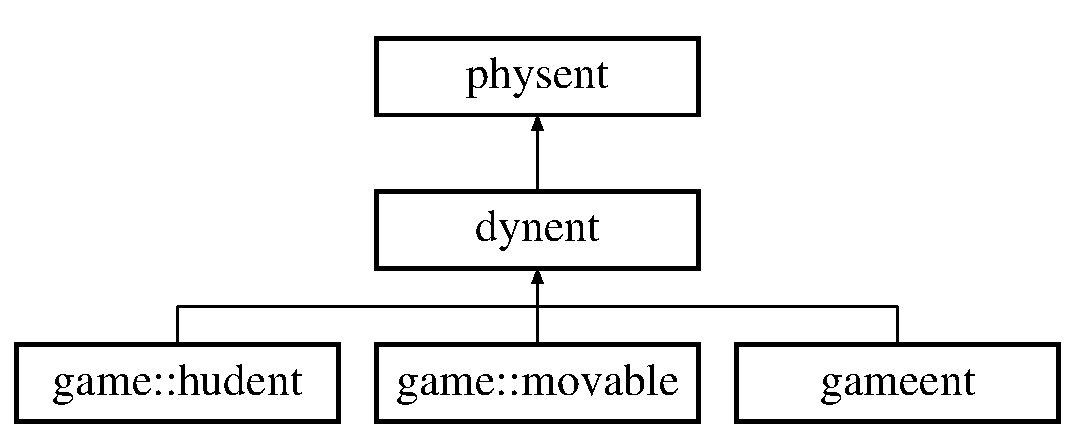
\includegraphics[height=3.000000cm]{structdynent}
\end{center}
\end{figure}
\subsection*{Public Member Functions}
\begin{DoxyCompactItemize}
\item 
\mbox{\Hypertarget{structdynent_a5aad02ec178807bec16f71b778e13857}\label{structdynent_a5aad02ec178807bec16f71b778e13857}} 
void {\bfseries stopmoving} ()
\item 
\mbox{\Hypertarget{structdynent_acf4e18ebbdad44d9c8ca4ca2a33e350f}\label{structdynent_acf4e18ebbdad44d9c8ca4ca2a33e350f}} 
void {\bfseries reset} ()
\item 
\mbox{\Hypertarget{structdynent_aab7f1db95239110fb0869f955e209e21}\label{structdynent_aab7f1db95239110fb0869f955e209e21}} 
\hyperlink{structvec}{vec} {\bfseries abovehead} ()
\end{DoxyCompactItemize}
\subsection*{Public Attributes}
\begin{DoxyCompactItemize}
\item 
\mbox{\Hypertarget{structdynent_a4d1a81af37056f80ad90cee60b9ecca8}\label{structdynent_a4d1a81af37056f80ad90cee60b9ecca8}} 
bool {\bfseries k\+\_\+left}
\item 
\mbox{\Hypertarget{structdynent_a328ca39121b002c30b585162adec026b}\label{structdynent_a328ca39121b002c30b585162adec026b}} 
bool {\bfseries k\+\_\+right}
\item 
\mbox{\Hypertarget{structdynent_afaa0d5d6115b157e1b9bf3d61ee42543}\label{structdynent_afaa0d5d6115b157e1b9bf3d61ee42543}} 
bool {\bfseries k\+\_\+up}
\item 
\mbox{\Hypertarget{structdynent_a093fb4ab684f252e4b315fbef20ee213}\label{structdynent_a093fb4ab684f252e4b315fbef20ee213}} 
bool {\bfseries k\+\_\+down}
\item 
\mbox{\Hypertarget{structdynent_a9dd2a14bdf3477051377b2764573f406}\label{structdynent_a9dd2a14bdf3477051377b2764573f406}} 
\hyperlink{structaniminterpinfo}{animinterpinfo} {\bfseries animinterp} \mbox{[}M\+A\+X\+A\+N\+I\+M\+P\+A\+R\+TS\mbox{]}
\item 
\mbox{\Hypertarget{structdynent_a044523da3ffad90441e3d79fae6d11e4}\label{structdynent_a044523da3ffad90441e3d79fae6d11e4}} 
\hyperlink{structragdolldata}{ragdolldata} $\ast$ {\bfseries ragdoll}
\item 
\mbox{\Hypertarget{structdynent_abf556f539cfdb81a5546764890a3b753}\label{structdynent_abf556f539cfdb81a5546764890a3b753}} 
\hyperlink{structoccludequery}{occludequery} $\ast$ {\bfseries query}
\item 
\mbox{\Hypertarget{structdynent_a51cc3ac02efb8eba47172bad12806c3d}\label{structdynent_a51cc3ac02efb8eba47172bad12806c3d}} 
int {\bfseries lastrendered}
\end{DoxyCompactItemize}


The documentation for this struct was generated from the following file\+:\begin{DoxyCompactItemize}
\item 
H\+:/\+Rival\+Engine/\+Rival\+\_\+\+Game\+\_\+\+Engine\+\_\+\+G\+I\+T/\+Rival3dengine/source/shared/ents.\+h\end{DoxyCompactItemize}

\hypertarget{structdynlight}{}\section{dynlight Struct Reference}
\label{structdynlight}\index{dynlight@{dynlight}}
\subsection*{Public Member Functions}
\begin{DoxyCompactItemize}
\item 
\mbox{\Hypertarget{structdynlight_aae27a9f01e6288f95140a6aba456b3c1}\label{structdynlight_aae27a9f01e6288f95140a6aba456b3c1}} 
void {\bfseries calcradius} ()
\item 
\mbox{\Hypertarget{structdynlight_aa5fa1fe1523322704c9fe3204ea124fe}\label{structdynlight_aa5fa1fe1523322704c9fe3204ea124fe}} 
void {\bfseries calccolor} ()
\end{DoxyCompactItemize}
\subsection*{Public Attributes}
\begin{DoxyCompactItemize}
\item 
\mbox{\Hypertarget{structdynlight_a9653404c14b1d0e32d2e8828d660742c}\label{structdynlight_a9653404c14b1d0e32d2e8828d660742c}} 
\hyperlink{structvec}{vec} {\bfseries o}
\item 
\mbox{\Hypertarget{structdynlight_a122bbd0bafea160d9eeba5211560f6f1}\label{structdynlight_a122bbd0bafea160d9eeba5211560f6f1}} 
\hyperlink{structvec}{vec} {\bfseries hud}
\item 
\mbox{\Hypertarget{structdynlight_a9529fb9f0f77c8c3f6f1a299a99bc61c}\label{structdynlight_a9529fb9f0f77c8c3f6f1a299a99bc61c}} 
float {\bfseries radius}
\item 
\mbox{\Hypertarget{structdynlight_a6b7f51b9ffe4d8f2661867827620da95}\label{structdynlight_a6b7f51b9ffe4d8f2661867827620da95}} 
float {\bfseries initradius}
\item 
\mbox{\Hypertarget{structdynlight_ab967625b00a9ec793391f0ac13178455}\label{structdynlight_ab967625b00a9ec793391f0ac13178455}} 
float {\bfseries curradius}
\item 
\mbox{\Hypertarget{structdynlight_ad6649de3370bb210766d3b6383437c1e}\label{structdynlight_ad6649de3370bb210766d3b6383437c1e}} 
float {\bfseries dist}
\item 
\mbox{\Hypertarget{structdynlight_a6aa71d24f1e9a102661d4de0948c4185}\label{structdynlight_a6aa71d24f1e9a102661d4de0948c4185}} 
\hyperlink{structvec}{vec} {\bfseries color}
\item 
\mbox{\Hypertarget{structdynlight_aaca94d9c273ca954af77be2f5b71ab37}\label{structdynlight_aaca94d9c273ca954af77be2f5b71ab37}} 
\hyperlink{structvec}{vec} {\bfseries initcolor}
\item 
\mbox{\Hypertarget{structdynlight_ad79d22be233ea7db75e10fea5fe94eb9}\label{structdynlight_ad79d22be233ea7db75e10fea5fe94eb9}} 
\hyperlink{structvec}{vec} {\bfseries curcolor}
\item 
\mbox{\Hypertarget{structdynlight_a7f8045a0dde58399ce1e2fefa7655227}\label{structdynlight_a7f8045a0dde58399ce1e2fefa7655227}} 
int {\bfseries fade}
\item 
\mbox{\Hypertarget{structdynlight_a92c6374dd0e08a13f7f2aad89a9dd26f}\label{structdynlight_a92c6374dd0e08a13f7f2aad89a9dd26f}} 
int {\bfseries peak}
\item 
\mbox{\Hypertarget{structdynlight_a0fec67692c1615ddf6ed5a536d3a1f4b}\label{structdynlight_a0fec67692c1615ddf6ed5a536d3a1f4b}} 
int {\bfseries expire}
\item 
\mbox{\Hypertarget{structdynlight_af87f9b9b13b59e73ec605e5f507bf8e8}\label{structdynlight_af87f9b9b13b59e73ec605e5f507bf8e8}} 
int {\bfseries flags}
\item 
\mbox{\Hypertarget{structdynlight_ac7d520548d1d9ec667859ccb9f3aa75a}\label{structdynlight_ac7d520548d1d9ec667859ccb9f3aa75a}} 
\hyperlink{structphysent}{physent} $\ast$ {\bfseries owner}
\item 
\mbox{\Hypertarget{structdynlight_a99a26e2fc3ba427615cf7c1c5a186d2a}\label{structdynlight_a99a26e2fc3ba427615cf7c1c5a186d2a}} 
\hyperlink{structvec}{vec} {\bfseries dir}
\item 
\mbox{\Hypertarget{structdynlight_ad09b70b225c9836e55a03e7c85bd043e}\label{structdynlight_ad09b70b225c9836e55a03e7c85bd043e}} 
int {\bfseries spot}
\end{DoxyCompactItemize}


The documentation for this struct was generated from the following file\+:\begin{DoxyCompactItemize}
\item 
H\+:/\+Rival\+Engine/\+Rival\+\_\+\+Game\+\_\+\+Engine\+\_\+\+G\+I\+T/\+Rival3dengine/source/engine/dynlight.\+cpp\end{DoxyCompactItemize}

\hypertarget{structecjacobian}{}\section{ecjacobian Struct Reference}
\label{structecjacobian}\index{ecjacobian@{ecjacobian}}
\subsection*{Public Member Functions}
\begin{DoxyCompactItemize}
\item 
\mbox{\Hypertarget{structecjacobian_a05218cdae34aaee8a61f8046452224fe}\label{structecjacobian_a05218cdae34aaee8a61f8046452224fe}} 
{\bfseries ecjacobian} (const \hyperlink{structgfield}{gfield} \&x, const \hyperlink{structgfield}{gfield} \&y)
\item 
\mbox{\Hypertarget{structecjacobian_ab7b28dee64ba750d1964bb38f2c4ef3e}\label{structecjacobian_ab7b28dee64ba750d1964bb38f2c4ef3e}} 
{\bfseries ecjacobian} (const \hyperlink{structgfield}{gfield} \&x, const \hyperlink{structgfield}{gfield} \&y, const \hyperlink{structgfield}{gfield} \&z)
\item 
\mbox{\Hypertarget{structecjacobian_af7b92c34cc52b270a8ca85dd124ddb2b}\label{structecjacobian_af7b92c34cc52b270a8ca85dd124ddb2b}} 
void {\bfseries mul2} ()
\item 
\mbox{\Hypertarget{structecjacobian_a8d0f54c79fb5e40433b75fc9ca895e87}\label{structecjacobian_a8d0f54c79fb5e40433b75fc9ca895e87}} 
void {\bfseries add} (const \hyperlink{structecjacobian}{ecjacobian} \&q)
\item 
\mbox{\Hypertarget{structecjacobian_a9da0182495ad309dcaf189a32c8de79c}\label{structecjacobian_a9da0182495ad309dcaf189a32c8de79c}} 
{\footnotesize template$<$int Q\+\_\+\+D\+I\+G\+I\+TS$>$ }\\void {\bfseries mul} (const \hyperlink{structecjacobian}{ecjacobian} \&p, const \hyperlink{structbigint}{bigint}$<$ Q\+\_\+\+D\+I\+G\+I\+TS $>$ \&q)
\item 
\mbox{\Hypertarget{structecjacobian_ae6f7f0bb6cc754cedfce1b3befb63b9b}\label{structecjacobian_ae6f7f0bb6cc754cedfce1b3befb63b9b}} 
{\footnotesize template$<$int Q\+\_\+\+D\+I\+G\+I\+TS$>$ }\\void {\bfseries mul} (const \hyperlink{structbigint}{bigint}$<$ Q\+\_\+\+D\+I\+G\+I\+TS $>$ \&q)
\item 
\mbox{\Hypertarget{structecjacobian_ad09a88474b98d2c327c6dca6f5ff6a6f}\label{structecjacobian_ad09a88474b98d2c327c6dca6f5ff6a6f}} 
void {\bfseries normalize} ()
\item 
\mbox{\Hypertarget{structecjacobian_a40a477b7acb8e9b0a6fa1656f5de9505}\label{structecjacobian_a40a477b7acb8e9b0a6fa1656f5de9505}} 
bool {\bfseries calcy} (bool ybit)
\item 
\mbox{\Hypertarget{structecjacobian_a3961d9ec5bc904dc559866471f9c4df2}\label{structecjacobian_a3961d9ec5bc904dc559866471f9c4df2}} 
void {\bfseries print} (\hyperlink{structvector}{vector}$<$ char $>$ \&buf)
\item 
\mbox{\Hypertarget{structecjacobian_a6f454e80faefed944a0238f0e0a96941}\label{structecjacobian_a6f454e80faefed944a0238f0e0a96941}} 
void {\bfseries parse} (const char $\ast$s)
\end{DoxyCompactItemize}
\subsection*{Public Attributes}
\begin{DoxyCompactItemize}
\item 
\mbox{\Hypertarget{structecjacobian_a2f81443c8b363b8a4983c55634bdb4b2}\label{structecjacobian_a2f81443c8b363b8a4983c55634bdb4b2}} 
\hyperlink{structgfield}{gfield} {\bfseries x}
\item 
\mbox{\Hypertarget{structecjacobian_abb5fa282ef4817537886493c49217b16}\label{structecjacobian_abb5fa282ef4817537886493c49217b16}} 
\hyperlink{structgfield}{gfield} {\bfseries y}
\item 
\mbox{\Hypertarget{structecjacobian_a3b9cb207ffa77ea4efca837c91952499}\label{structecjacobian_a3b9cb207ffa77ea4efca837c91952499}} 
\hyperlink{structgfield}{gfield} {\bfseries z}
\end{DoxyCompactItemize}
\subsection*{Static Public Attributes}
\begin{DoxyCompactItemize}
\item 
\mbox{\Hypertarget{structecjacobian_a987dc64d4f39332c3536f4d1a4264abb}\label{structecjacobian_a987dc64d4f39332c3536f4d1a4264abb}} 
static const \hyperlink{structgfield}{gfield} {\bfseries B}
\item 
\mbox{\Hypertarget{structecjacobian_af53d82b93db9e3f054b16010306d5141}\label{structecjacobian_af53d82b93db9e3f054b16010306d5141}} 
static const \hyperlink{structecjacobian}{ecjacobian} {\bfseries base}
\item 
\mbox{\Hypertarget{structecjacobian_a760e477cb6b7ec8a01e672832cd1ee2b}\label{structecjacobian_a760e477cb6b7ec8a01e672832cd1ee2b}} 
static const \hyperlink{structecjacobian}{ecjacobian} {\bfseries origin}
\end{DoxyCompactItemize}


The documentation for this struct was generated from the following file\+:\begin{DoxyCompactItemize}
\item 
H\+:/\+Rival\+Engine/\+Rival\+\_\+\+Game\+\_\+\+Engine\+\_\+\+G\+I\+T/\+Rival3dengine/source/shared/crypto.\+cpp\end{DoxyCompactItemize}

\hypertarget{structedgegroup}{}\section{edgegroup Struct Reference}
\label{structedgegroup}\index{edgegroup@{edgegroup}}
\subsection*{Public Attributes}
\begin{DoxyCompactItemize}
\item 
\mbox{\Hypertarget{structedgegroup_ab10c667196232f99e71f6fdc864bf519}\label{structedgegroup_ab10c667196232f99e71f6fdc864bf519}} 
\hyperlink{structivec}{ivec} {\bfseries slope}
\item 
\mbox{\Hypertarget{structedgegroup_a68564d72dcf2555be453ed4de1d43cc0}\label{structedgegroup_a68564d72dcf2555be453ed4de1d43cc0}} 
\hyperlink{structivec}{ivec} {\bfseries origin}
\item 
\mbox{\Hypertarget{structedgegroup_ab864d927422ec195e2a4fa04e932231b}\label{structedgegroup_ab864d927422ec195e2a4fa04e932231b}} 
int {\bfseries axis}
\end{DoxyCompactItemize}


The documentation for this struct was generated from the following file\+:\begin{DoxyCompactItemize}
\item 
H\+:/\+Rival\+Engine/\+Rival\+\_\+\+Game\+\_\+\+Engine\+\_\+\+G\+I\+T/\+Rival3dengine/source/engine/octarender.\+cpp\end{DoxyCompactItemize}

\hypertarget{structeditinfo}{}\section{editinfo Struct Reference}
\label{structeditinfo}\index{editinfo@{editinfo}}
Inheritance diagram for editinfo\+:\begin{figure}[H]
\begin{center}
\leavevmode
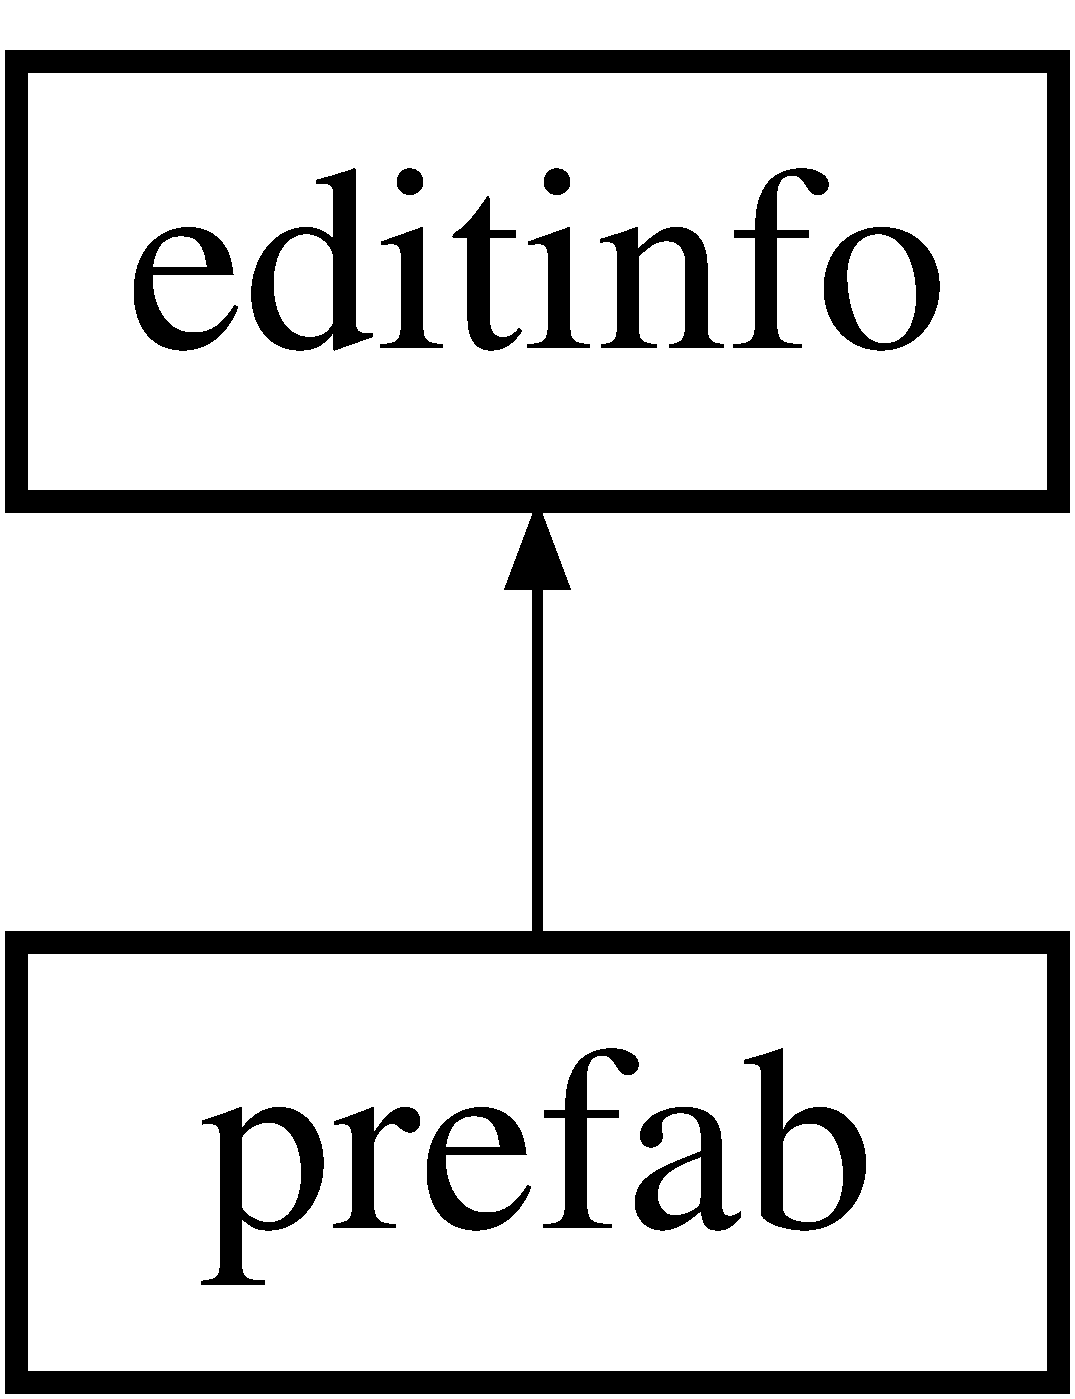
\includegraphics[height=2.000000cm]{structeditinfo}
\end{center}
\end{figure}
\subsection*{Public Attributes}
\begin{DoxyCompactItemize}
\item 
\mbox{\Hypertarget{structeditinfo_aa289d6d9d860f4d343a0ef6645ed3cb6}\label{structeditinfo_aa289d6d9d860f4d343a0ef6645ed3cb6}} 
\hyperlink{structblock3}{block3} $\ast$ {\bfseries copy}
\end{DoxyCompactItemize}


The documentation for this struct was generated from the following file\+:\begin{DoxyCompactItemize}
\item 
H\+:/\+Rival\+Engine/\+Rival\+\_\+\+Game\+\_\+\+Engine\+\_\+\+G\+I\+T/\+Rival3dengine/source/engine/octa.\+h\end{DoxyCompactItemize}

\hypertarget{structeditline}{}\section{editline Struct Reference}
\label{structeditline}\index{editline@{editline}}
\subsection*{Public Types}
\begin{DoxyCompactItemize}
\item 
\mbox{\Hypertarget{structeditline_a3d4a39e526697d6f73dcfeede8245545}\label{structeditline_a3d4a39e526697d6f73dcfeede8245545}} 
enum \{ {\bfseries C\+H\+U\+N\+K\+S\+I\+ZE} = 256
 \}
\end{DoxyCompactItemize}
\subsection*{Public Member Functions}
\begin{DoxyCompactItemize}
\item 
\mbox{\Hypertarget{structeditline_aaa101a9248d101995d593667581e4996}\label{structeditline_aaa101a9248d101995d593667581e4996}} 
{\bfseries editline} (const char $\ast$init)
\item 
\mbox{\Hypertarget{structeditline_aff8a51dd9a54c65b674bc86bfa1566a9}\label{structeditline_aff8a51dd9a54c65b674bc86bfa1566a9}} 
bool {\bfseries empty} ()
\item 
\mbox{\Hypertarget{structeditline_a22d5497ef592e0df789e50288e9cddc9}\label{structeditline_a22d5497ef592e0df789e50288e9cddc9}} 
void {\bfseries clear} ()
\item 
\mbox{\Hypertarget{structeditline_ad265849bc6b8e6d587b16be5fc7b47bb}\label{structeditline_ad265849bc6b8e6d587b16be5fc7b47bb}} 
bool {\bfseries grow} (int total, const char $\ast$fmt=\char`\"{}\char`\"{},...)
\item 
\mbox{\Hypertarget{structeditline_a68cad302d8daf88381753bbaeb3a6681}\label{structeditline_a68cad302d8daf88381753bbaeb3a6681}} 
void {\bfseries set} (const char $\ast$str, int slen=-\/1)
\item 
\mbox{\Hypertarget{structeditline_a52837ff76228fbd8935117096475cd93}\label{structeditline_a52837ff76228fbd8935117096475cd93}} 
void {\bfseries prepend} (const char $\ast$str)
\item 
\mbox{\Hypertarget{structeditline_a389153edfce8843acac521157380300c}\label{structeditline_a389153edfce8843acac521157380300c}} 
void {\bfseries append} (const char $\ast$str)
\item 
\mbox{\Hypertarget{structeditline_a80640b49f44eb8a0492135716c0df5f7}\label{structeditline_a80640b49f44eb8a0492135716c0df5f7}} 
bool {\bfseries read} (\hyperlink{structstream}{stream} $\ast$f, int chop=-\/1)
\item 
\mbox{\Hypertarget{structeditline_aac1676e4f0579285cd16f585a465dec0}\label{structeditline_aac1676e4f0579285cd16f585a465dec0}} 
void {\bfseries del} (int start, int count)
\item 
\mbox{\Hypertarget{structeditline_a5ab95cb33794ff819377b04a54722ff3}\label{structeditline_a5ab95cb33794ff819377b04a54722ff3}} 
void {\bfseries chop} (int newlen)
\item 
\mbox{\Hypertarget{structeditline_a01fb8b60099754c85e2c2941e6c1da53}\label{structeditline_a01fb8b60099754c85e2c2941e6c1da53}} 
void {\bfseries insert} (char $\ast$str, int start, int count=0)
\item 
\mbox{\Hypertarget{structeditline_a0e1a2086b6f1ff1f571878b8df38e9ea}\label{structeditline_a0e1a2086b6f1ff1f571878b8df38e9ea}} 
void {\bfseries combinelines} (\hyperlink{structvector}{vector}$<$ \hyperlink{structeditline}{editline} $>$ \&src)
\end{DoxyCompactItemize}
\subsection*{Public Attributes}
\begin{DoxyCompactItemize}
\item 
\mbox{\Hypertarget{structeditline_aca6722eaec92a332e2f5f19a0218346f}\label{structeditline_aca6722eaec92a332e2f5f19a0218346f}} 
char $\ast$ {\bfseries text}
\item 
\mbox{\Hypertarget{structeditline_aedf4d62cf6b138c761b9f1bb2df3fdba}\label{structeditline_aedf4d62cf6b138c761b9f1bb2df3fdba}} 
int {\bfseries len}
\item 
\mbox{\Hypertarget{structeditline_abec5185ee12832521ad20127df5f818d}\label{structeditline_abec5185ee12832521ad20127df5f818d}} 
int {\bfseries maxlen}
\end{DoxyCompactItemize}


The documentation for this struct was generated from the following file\+:\begin{DoxyCompactItemize}
\item 
H\+:/\+Rival\+Engine/\+Rival\+\_\+\+Game\+\_\+\+Engine\+\_\+\+G\+I\+T/\+Rival3dengine/source/engine/textedit.\+h\end{DoxyCompactItemize}

\hypertarget{structeditor}{}\section{editor Struct Reference}
\label{structeditor}\index{editor@{editor}}
\subsection*{Public Member Functions}
\begin{DoxyCompactItemize}
\item 
\mbox{\Hypertarget{structeditor_a73d800d5ae8e42c056166ad8fd9f0d09}\label{structeditor_a73d800d5ae8e42c056166ad8fd9f0d09}} 
{\bfseries editor} (const char $\ast$name, int mode, const char $\ast$initval)
\item 
\mbox{\Hypertarget{structeditor_ae824bd24fcdcb69208c791f7cbcfdd33}\label{structeditor_ae824bd24fcdcb69208c791f7cbcfdd33}} 
bool {\bfseries empty} ()
\item 
\mbox{\Hypertarget{structeditor_a5ec80a331e365c594c15e7ae3e587b39}\label{structeditor_a5ec80a331e365c594c15e7ae3e587b39}} 
void {\bfseries clear} (const char $\ast$init=\char`\"{}\char`\"{})
\item 
\mbox{\Hypertarget{structeditor_ac88f39c72c21bea2c1cef32533f5f5ca}\label{structeditor_ac88f39c72c21bea2c1cef32533f5f5ca}} 
void {\bfseries init} (const char $\ast$inittext)
\item 
\mbox{\Hypertarget{structeditor_a412c70983695801aa20629f732bbace0}\label{structeditor_a412c70983695801aa20629f732bbace0}} 
void {\bfseries updateheight} ()
\item 
\mbox{\Hypertarget{structeditor_ae7966c2485d7670f580b632fc35768ee}\label{structeditor_ae7966c2485d7670f580b632fc35768ee}} 
void {\bfseries setfile} (const char $\ast$fname)
\item 
\mbox{\Hypertarget{structeditor_a2d507562b7e1ec359303c00f8d52a9cd}\label{structeditor_a2d507562b7e1ec359303c00f8d52a9cd}} 
void {\bfseries load} ()
\item 
\mbox{\Hypertarget{structeditor_a9f4fc95fea744a815c8bf0a42b2cef9a}\label{structeditor_a9f4fc95fea744a815c8bf0a42b2cef9a}} 
void {\bfseries save} ()
\item 
\mbox{\Hypertarget{structeditor_a05196453980b40d4e831c23fc56c0f25}\label{structeditor_a05196453980b40d4e831c23fc56c0f25}} 
void {\bfseries mark} (bool enable)
\item 
\mbox{\Hypertarget{structeditor_aa53a80499cfc20776b37a20b5a1ff45f}\label{structeditor_aa53a80499cfc20776b37a20b5a1ff45f}} 
void {\bfseries selectall} ()
\item 
\mbox{\Hypertarget{structeditor_a2b2e4cd80ab8e735ce72c5bb0086dff5}\label{structeditor_a2b2e4cd80ab8e735ce72c5bb0086dff5}} 
bool {\bfseries region} (int \&sx, int \&sy, int \&ex, int \&ey)
\item 
\mbox{\Hypertarget{structeditor_af206725c53188ae8c71057b04a6966bd}\label{structeditor_af206725c53188ae8c71057b04a6966bd}} 
bool {\bfseries region} ()
\item 
\mbox{\Hypertarget{structeditor_a044ffeb175cc4f070ad48c3d9d789cd6}\label{structeditor_a044ffeb175cc4f070ad48c3d9d789cd6}} 
\hyperlink{structeditline}{editline} \& {\bfseries currentline} ()
\item 
\mbox{\Hypertarget{structeditor_a332d998647823fe5429dc9f431dac87b}\label{structeditor_a332d998647823fe5429dc9f431dac87b}} 
void {\bfseries copyselectionto} (\hyperlink{structeditor}{editor} $\ast$b)
\item 
\mbox{\Hypertarget{structeditor_a67c852303cea937e79f07b85e43851de}\label{structeditor_a67c852303cea937e79f07b85e43851de}} 
char $\ast$ {\bfseries tostring} ()
\item 
\mbox{\Hypertarget{structeditor_a6f1384db9c58b4b3758aa89dd55d05df}\label{structeditor_a6f1384db9c58b4b3758aa89dd55d05df}} 
char $\ast$ {\bfseries selectiontostring} ()
\item 
\mbox{\Hypertarget{structeditor_a65463dc6d9210bdb69be40f63a0a7ffe}\label{structeditor_a65463dc6d9210bdb69be40f63a0a7ffe}} 
void {\bfseries removelines} (int start, int count)
\item 
\mbox{\Hypertarget{structeditor_ab456c9f04564795c90f52c3ecb2b22d0}\label{structeditor_ab456c9f04564795c90f52c3ecb2b22d0}} 
bool {\bfseries del} ()
\item 
\mbox{\Hypertarget{structeditor_a9d79191f8b3ccddccd8b083ad0a9e3dd}\label{structeditor_a9d79191f8b3ccddccd8b083ad0a9e3dd}} 
void {\bfseries insert} (char ch)
\item 
\mbox{\Hypertarget{structeditor_a382e17bd2853bec918fdd8158ddc0c0d}\label{structeditor_a382e17bd2853bec918fdd8158ddc0c0d}} 
void {\bfseries insert} (const char $\ast$s)
\item 
\mbox{\Hypertarget{structeditor_a4524cdbc7b3bcc631c85c3d1fd89fa99}\label{structeditor_a4524cdbc7b3bcc631c85c3d1fd89fa99}} 
void {\bfseries insertallfrom} (\hyperlink{structeditor}{editor} $\ast$b)
\item 
\mbox{\Hypertarget{structeditor_a0891d5a364871c199fe38e3c2e85815f}\label{structeditor_a0891d5a364871c199fe38e3c2e85815f}} 
void {\bfseries scrollup} ()
\item 
\mbox{\Hypertarget{structeditor_a6173910e8a38625de244256ece5ee40f}\label{structeditor_a6173910e8a38625de244256ece5ee40f}} 
void {\bfseries scrolldown} ()
\item 
\mbox{\Hypertarget{structeditor_aec26a5e5780a67244ae7edef506bc967}\label{structeditor_aec26a5e5780a67244ae7edef506bc967}} 
void {\bfseries key} (int code)
\item 
\mbox{\Hypertarget{structeditor_aceb6a8299b0181d2b88e6439bc5b1d27}\label{structeditor_aceb6a8299b0181d2b88e6439bc5b1d27}} 
void {\bfseries input} (const char $\ast$str, int len)
\item 
\mbox{\Hypertarget{structeditor_afea643d1c4eba985b6978b228a15f957}\label{structeditor_afea643d1c4eba985b6978b228a15f957}} 
void {\bfseries hit} (int hitx, int hity, bool dragged)
\item 
\mbox{\Hypertarget{structeditor_a61d3b1198c453856c3ae69ce2c92b036}\label{structeditor_a61d3b1198c453856c3ae69ce2c92b036}} 
int {\bfseries limitscrolly} ()
\item 
\mbox{\Hypertarget{structeditor_addadc273617926d876d009c29b3440ae}\label{structeditor_addadc273617926d876d009c29b3440ae}} 
void {\bfseries draw} (int x, int y, int color, bool hit)
\end{DoxyCompactItemize}
\subsection*{Public Attributes}
\begin{DoxyCompactItemize}
\item 
\mbox{\Hypertarget{structeditor_a28a82e6cd5f3f9ddfff752cabe7ad1ef}\label{structeditor_a28a82e6cd5f3f9ddfff752cabe7ad1ef}} 
int {\bfseries mode}
\item 
\mbox{\Hypertarget{structeditor_afbae92cf046700ca6e65eca8d470ede7}\label{structeditor_afbae92cf046700ca6e65eca8d470ede7}} 
bool {\bfseries active}
\item 
\mbox{\Hypertarget{structeditor_a9a4395bb5cb85cc2d534c251ffa52bea}\label{structeditor_a9a4395bb5cb85cc2d534c251ffa52bea}} 
bool {\bfseries rendered}
\item 
\mbox{\Hypertarget{structeditor_a22f369dd45964527fa9cfdb8cd01e28b}\label{structeditor_a22f369dd45964527fa9cfdb8cd01e28b}} 
const char $\ast$ {\bfseries name}
\item 
\mbox{\Hypertarget{structeditor_a98b321e8ecd8cc9dc802233d7c5d2253}\label{structeditor_a98b321e8ecd8cc9dc802233d7c5d2253}} 
const char $\ast$ {\bfseries filename}
\item 
\mbox{\Hypertarget{structeditor_a3555bb91667bd7825daa738ffe800239}\label{structeditor_a3555bb91667bd7825daa738ffe800239}} 
int {\bfseries cx}
\item 
\mbox{\Hypertarget{structeditor_a2ab02b4d78fe909b6f2c1c8b55969bdd}\label{structeditor_a2ab02b4d78fe909b6f2c1c8b55969bdd}} 
int {\bfseries cy}
\item 
\mbox{\Hypertarget{structeditor_ad47e36e2479ec1ad5b8c33aa5bdeebb9}\label{structeditor_ad47e36e2479ec1ad5b8c33aa5bdeebb9}} 
int {\bfseries mx}
\item 
\mbox{\Hypertarget{structeditor_a5759712451f062dc5942aa1d452c4b57}\label{structeditor_a5759712451f062dc5942aa1d452c4b57}} 
int {\bfseries my}
\item 
\mbox{\Hypertarget{structeditor_a2b728cc5938b2dc0acda99554628b5f1}\label{structeditor_a2b728cc5938b2dc0acda99554628b5f1}} 
int {\bfseries maxx}
\item 
\mbox{\Hypertarget{structeditor_ad318edcb8171bc7d56852cab53002395}\label{structeditor_ad318edcb8171bc7d56852cab53002395}} 
int {\bfseries maxy}
\item 
\mbox{\Hypertarget{structeditor_a3ab0fe5870f10f8dd7471122a3bbc2a6}\label{structeditor_a3ab0fe5870f10f8dd7471122a3bbc2a6}} 
int {\bfseries scrolly}
\item 
\mbox{\Hypertarget{structeditor_a37594098ee488498295473f3295ce646}\label{structeditor_a37594098ee488498295473f3295ce646}} 
bool {\bfseries linewrap}
\item 
\mbox{\Hypertarget{structeditor_a139a8e5b3f2e85ea95c3f38f92e8e82a}\label{structeditor_a139a8e5b3f2e85ea95c3f38f92e8e82a}} 
int {\bfseries pixelwidth}
\item 
\mbox{\Hypertarget{structeditor_a44929d2a5da7cfebda79c7673a95e34e}\label{structeditor_a44929d2a5da7cfebda79c7673a95e34e}} 
int {\bfseries pixelheight}
\item 
\mbox{\Hypertarget{structeditor_a3fa0c216055a1c485d8f443122a2d083}\label{structeditor_a3fa0c216055a1c485d8f443122a2d083}} 
\hyperlink{structvector}{vector}$<$ \hyperlink{structeditline}{editline} $>$ {\bfseries lines}
\end{DoxyCompactItemize}


The documentation for this struct was generated from the following file\+:\begin{DoxyCompactItemize}
\item 
H\+:/\+Rival\+Engine/\+Rival\+\_\+\+Game\+\_\+\+Engine\+\_\+\+G\+I\+T/\+Rival3dengine/source/engine/textedit.\+h\end{DoxyCompactItemize}

\hypertarget{structelementset}{}\section{elementset Struct Reference}
\label{structelementset}\index{elementset@{elementset}}
\subsection*{Public Attributes}
\begin{DoxyCompactItemize}
\item 
\mbox{\Hypertarget{structelementset_ad9e921699e354c4b38f8f582aea48a32}\label{structelementset_ad9e921699e354c4b38f8f582aea48a32}} 
ushort {\bfseries texture}
\item 
\mbox{\Hypertarget{structelementset_add673a9cfbe9161c7585264abf600838}\label{structelementset_add673a9cfbe9161c7585264abf600838}} 
ushort {\bfseries envmap}
\item 
\mbox{\Hypertarget{structelementset_aff80cf1b52eece3114c2a63c4c48cc75}\label{structelementset_aff80cf1b52eece3114c2a63c4c48cc75}} 
\begin{tabbing}
xx\=xx\=xx\=xx\=xx\=xx\=xx\=xx\=xx\=\kill
union \{\\
\mbox{\Hypertarget{unionelementset_1_1_0D41_a1bcc18959a1c62a17df4bcb93e318f98}\label{unionelementset_1_1_0D41_a1bcc18959a1c62a17df4bcb93e318f98}} 
\>struct \{\\
\>\>uchar {\bfseries orient}\\
\>\>uchar {\bfseries layer}\\
\>\} \\
\>ushort {\bfseries reuse}\\
\}; \\

\end{tabbing}\item 
\mbox{\Hypertarget{structelementset_a8fbb5ad3d066b997c182bda1c4416e97}\label{structelementset_a8fbb5ad3d066b997c182bda1c4416e97}} 
ushort {\bfseries length}
\item 
\mbox{\Hypertarget{structelementset_ac07809a40ba539f3e9190661ee7f9efb}\label{structelementset_ac07809a40ba539f3e9190661ee7f9efb}} 
ushort {\bfseries minvert}
\item 
\mbox{\Hypertarget{structelementset_a2a1e83e8c8e2668133822af4b199c605}\label{structelementset_a2a1e83e8c8e2668133822af4b199c605}} 
ushort {\bfseries maxvert}
\end{DoxyCompactItemize}


The documentation for this struct was generated from the following file\+:\begin{DoxyCompactItemize}
\item 
H\+:/\+Rival\+Engine/\+Rival\+\_\+\+Game\+\_\+\+Engine\+\_\+\+G\+I\+T/\+Rival3dengine/source/engine/octa.\+h\end{DoxyCompactItemize}

\hypertarget{structmpr_1_1_ent}{}\section{mpr\+:\+:Ent Struct Reference}
\label{structmpr_1_1_ent}\index{mpr\+::\+Ent@{mpr\+::\+Ent}}
Inheritance diagram for mpr\+:\+:Ent\+:\begin{figure}[H]
\begin{center}
\leavevmode
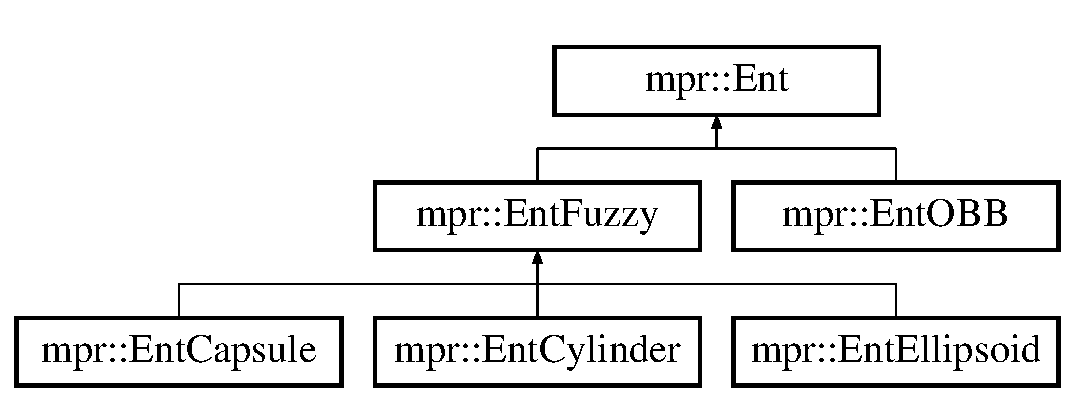
\includegraphics[height=3.000000cm]{structmpr_1_1_ent}
\end{center}
\end{figure}
\subsection*{Public Member Functions}
\begin{DoxyCompactItemize}
\item 
\mbox{\Hypertarget{structmpr_1_1_ent_aa25c314a245c2de3910ccec8b77868d5}\label{structmpr_1_1_ent_aa25c314a245c2de3910ccec8b77868d5}} 
{\bfseries Ent} (\hyperlink{structphysent}{physent} $\ast$ent)
\item 
\mbox{\Hypertarget{structmpr_1_1_ent_a29f53969d8f5d7cb74a45cf9bef4170e}\label{structmpr_1_1_ent_a29f53969d8f5d7cb74a45cf9bef4170e}} 
\hyperlink{structvec}{vec} {\bfseries center} () const
\end{DoxyCompactItemize}
\subsection*{Public Attributes}
\begin{DoxyCompactItemize}
\item 
\mbox{\Hypertarget{structmpr_1_1_ent_ab476bffba727c202b95365678c03280e}\label{structmpr_1_1_ent_ab476bffba727c202b95365678c03280e}} 
\hyperlink{structphysent}{physent} $\ast$ {\bfseries ent}
\end{DoxyCompactItemize}


The documentation for this struct was generated from the following file\+:\begin{DoxyCompactItemize}
\item 
H\+:/\+Rival\+Engine/\+Rival\+\_\+\+Game\+\_\+\+Engine\+\_\+\+G\+I\+T/\+Rival3dengine/source/engine/mpr.\+h\end{DoxyCompactItemize}

\hypertarget{structmpr_1_1_ent_capsule}{}\section{mpr\+:\+:Ent\+Capsule Struct Reference}
\label{structmpr_1_1_ent_capsule}\index{mpr\+::\+Ent\+Capsule@{mpr\+::\+Ent\+Capsule}}
Inheritance diagram for mpr\+:\+:Ent\+Capsule\+:\begin{figure}[H]
\begin{center}
\leavevmode
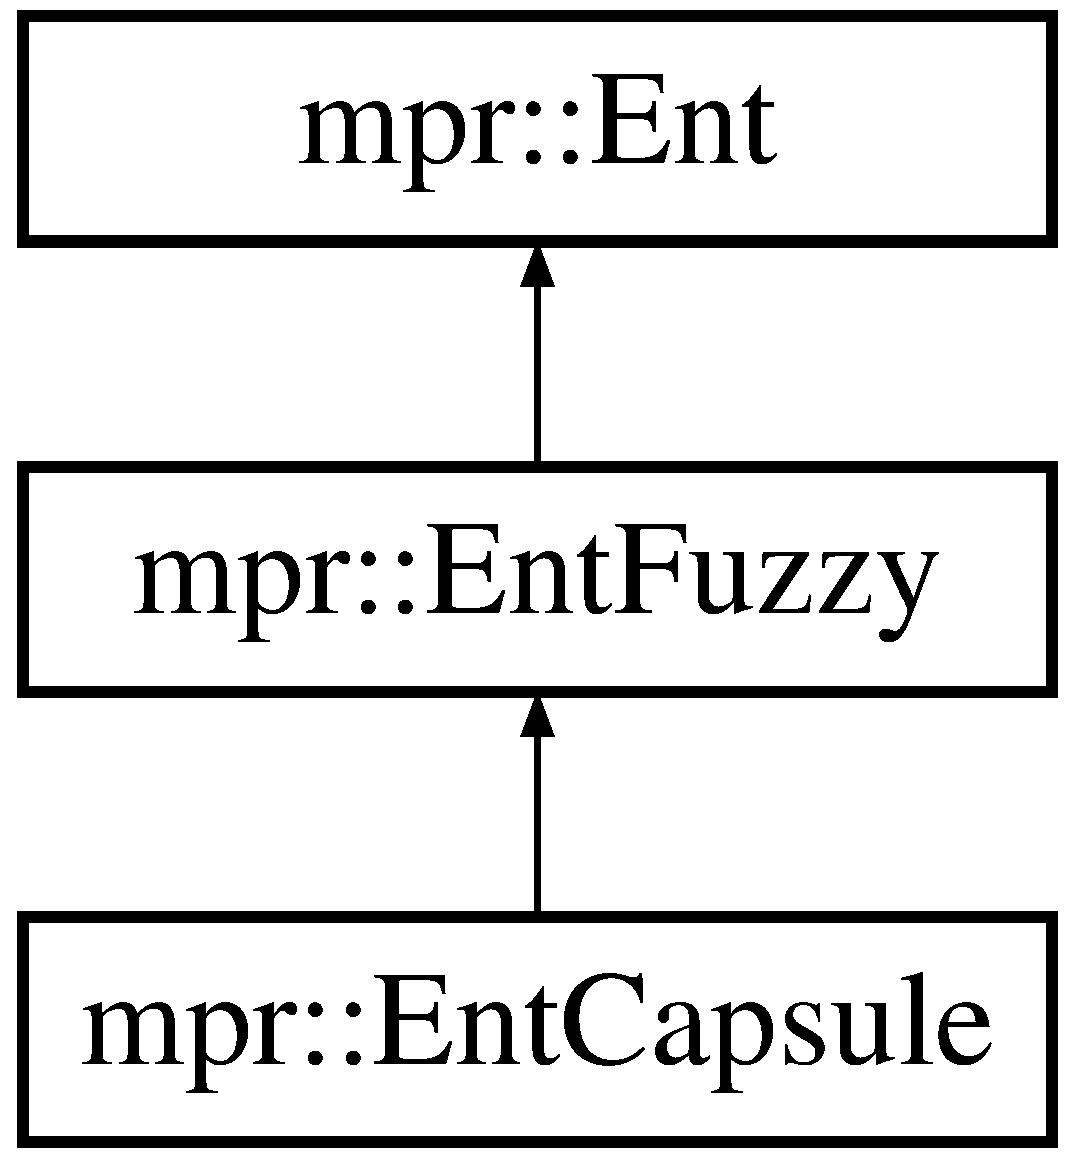
\includegraphics[height=3.000000cm]{structmpr_1_1_ent_capsule}
\end{center}
\end{figure}
\subsection*{Public Member Functions}
\begin{DoxyCompactItemize}
\item 
\mbox{\Hypertarget{structmpr_1_1_ent_capsule_add2b3d9bd9bd815883c26a477bf63943}\label{structmpr_1_1_ent_capsule_add2b3d9bd9bd815883c26a477bf63943}} 
{\bfseries Ent\+Capsule} (\hyperlink{structphysent}{physent} $\ast$ent)
\item 
\mbox{\Hypertarget{structmpr_1_1_ent_capsule_a506d3e637201e76b7433e8447e897dc8}\label{structmpr_1_1_ent_capsule_a506d3e637201e76b7433e8447e897dc8}} 
\hyperlink{structvec}{vec} {\bfseries supportpoint} (const \hyperlink{structvec}{vec} \&n) const
\end{DoxyCompactItemize}
\subsection*{Additional Inherited Members}


The documentation for this struct was generated from the following file\+:\begin{DoxyCompactItemize}
\item 
H\+:/\+Rival\+Engine/\+Rival\+\_\+\+Game\+\_\+\+Engine\+\_\+\+G\+I\+T/\+Rival3dengine/source/engine/mpr.\+h\end{DoxyCompactItemize}

\hypertarget{structmpr_1_1_ent_cylinder}{}\section{mpr\+:\+:Ent\+Cylinder Struct Reference}
\label{structmpr_1_1_ent_cylinder}\index{mpr\+::\+Ent\+Cylinder@{mpr\+::\+Ent\+Cylinder}}
Inheritance diagram for mpr\+:\+:Ent\+Cylinder\+:\begin{figure}[H]
\begin{center}
\leavevmode
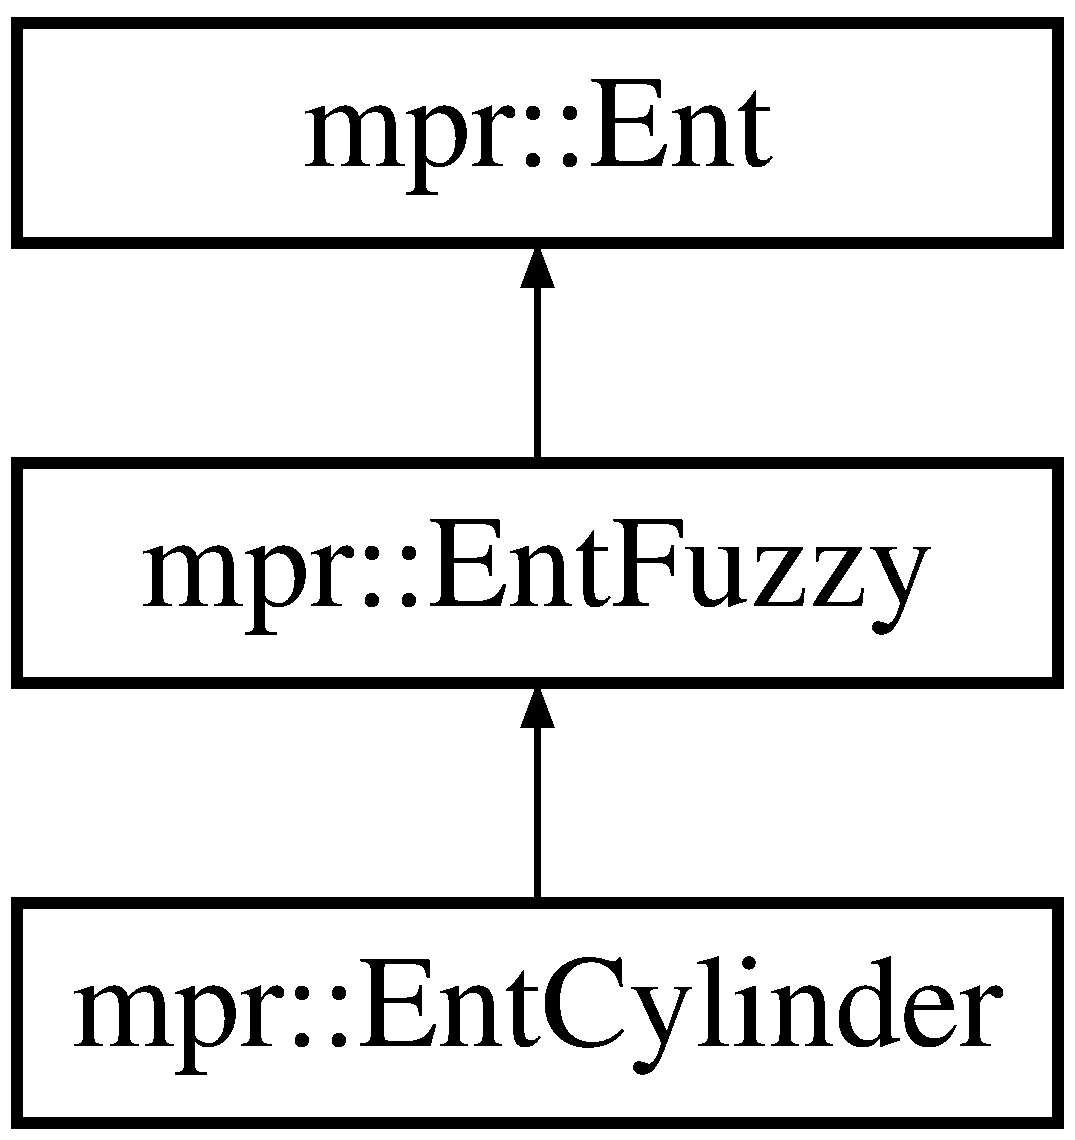
\includegraphics[height=3.000000cm]{structmpr_1_1_ent_cylinder}
\end{center}
\end{figure}
\subsection*{Public Member Functions}
\begin{DoxyCompactItemize}
\item 
\mbox{\Hypertarget{structmpr_1_1_ent_cylinder_a7dd91820b727dc2c861b2da439980cee}\label{structmpr_1_1_ent_cylinder_a7dd91820b727dc2c861b2da439980cee}} 
{\bfseries Ent\+Cylinder} (\hyperlink{structphysent}{physent} $\ast$ent, float zmargin=0)
\item 
\mbox{\Hypertarget{structmpr_1_1_ent_cylinder_aa8b1fa57929c4ec2a6dec0729887b697}\label{structmpr_1_1_ent_cylinder_aa8b1fa57929c4ec2a6dec0729887b697}} 
\hyperlink{structvec}{vec} {\bfseries center} () const
\item 
\mbox{\Hypertarget{structmpr_1_1_ent_cylinder_a38bd1c8a01b05403a3feacffe75a3f9c}\label{structmpr_1_1_ent_cylinder_a38bd1c8a01b05403a3feacffe75a3f9c}} 
float {\bfseries bottom} () const
\item 
\mbox{\Hypertarget{structmpr_1_1_ent_cylinder_a27f062f403e77e7b6341b87d0bc83fad}\label{structmpr_1_1_ent_cylinder_a27f062f403e77e7b6341b87d0bc83fad}} 
\hyperlink{structvec}{vec} {\bfseries contactface} (const \hyperlink{structvec}{vec} \&n, const \hyperlink{structvec}{vec} \&dir) const
\item 
\mbox{\Hypertarget{structmpr_1_1_ent_cylinder_a2fd84a92be8dd83bb553c823b82989d6}\label{structmpr_1_1_ent_cylinder_a2fd84a92be8dd83bb553c823b82989d6}} 
\hyperlink{structvec}{vec} {\bfseries supportpoint} (const \hyperlink{structvec}{vec} \&n) const
\end{DoxyCompactItemize}
\subsection*{Public Attributes}
\begin{DoxyCompactItemize}
\item 
\mbox{\Hypertarget{structmpr_1_1_ent_cylinder_a86b002f1e3a20229d5e241e90ca3a6b0}\label{structmpr_1_1_ent_cylinder_a86b002f1e3a20229d5e241e90ca3a6b0}} 
float {\bfseries zmargin}
\end{DoxyCompactItemize}


The documentation for this struct was generated from the following file\+:\begin{DoxyCompactItemize}
\item 
H\+:/\+Rival\+Engine/\+Rival\+\_\+\+Game\+\_\+\+Engine\+\_\+\+G\+I\+T/\+Rival3dengine/source/engine/mpr.\+h\end{DoxyCompactItemize}

\hypertarget{structmpr_1_1_ent_ellipsoid}{}\section{mpr\+:\+:Ent\+Ellipsoid Struct Reference}
\label{structmpr_1_1_ent_ellipsoid}\index{mpr\+::\+Ent\+Ellipsoid@{mpr\+::\+Ent\+Ellipsoid}}
Inheritance diagram for mpr\+:\+:Ent\+Ellipsoid\+:\begin{figure}[H]
\begin{center}
\leavevmode
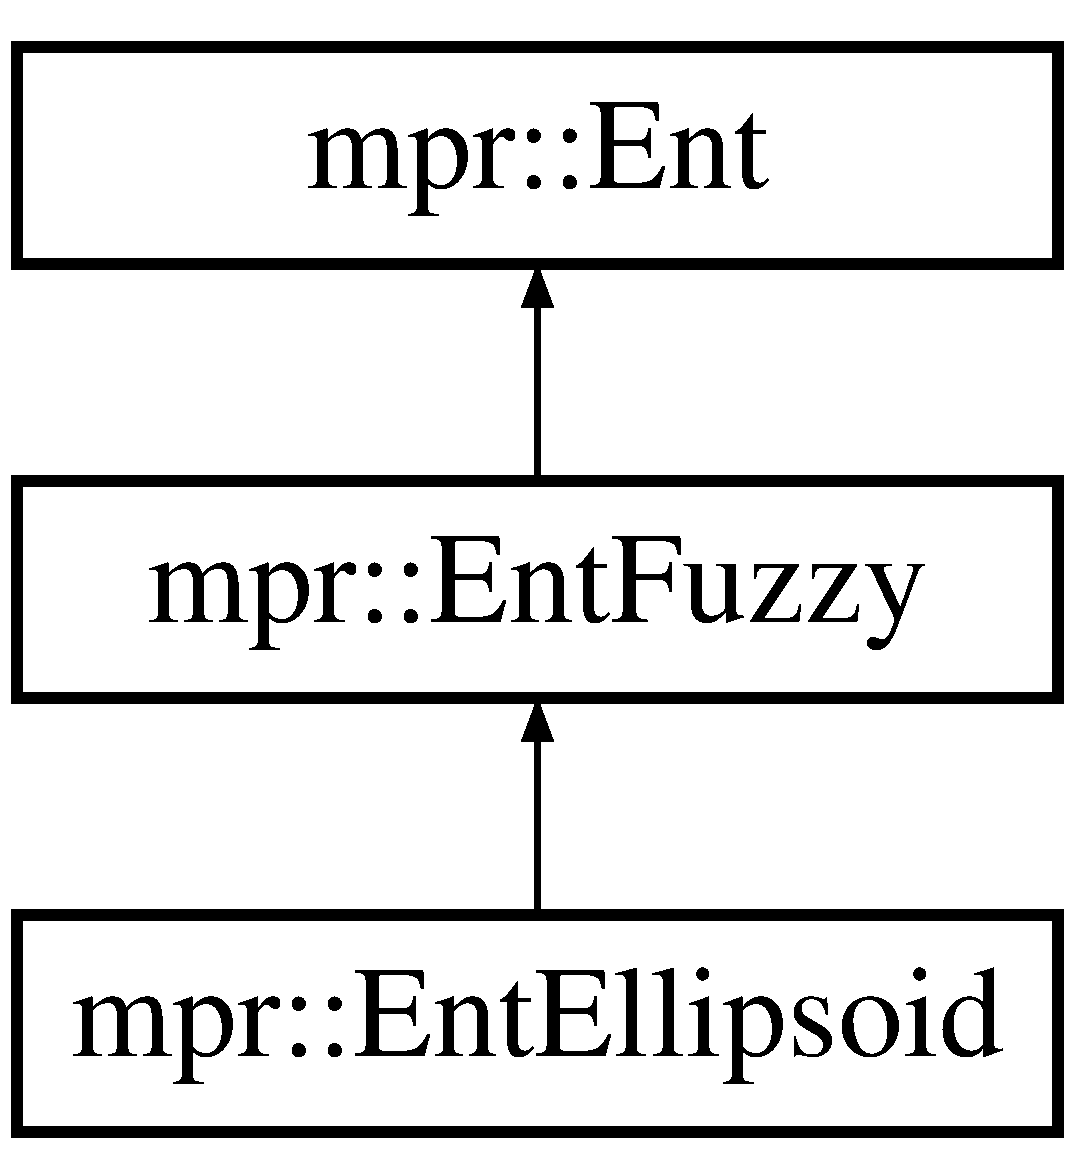
\includegraphics[height=3.000000cm]{structmpr_1_1_ent_ellipsoid}
\end{center}
\end{figure}
\subsection*{Public Member Functions}
\begin{DoxyCompactItemize}
\item 
\mbox{\Hypertarget{structmpr_1_1_ent_ellipsoid_a2189ddd0bfa43e49c2a1c1d6ef55f6d1}\label{structmpr_1_1_ent_ellipsoid_a2189ddd0bfa43e49c2a1c1d6ef55f6d1}} 
{\bfseries Ent\+Ellipsoid} (\hyperlink{structphysent}{physent} $\ast$ent)
\item 
\mbox{\Hypertarget{structmpr_1_1_ent_ellipsoid_a6ff3f1827252adbb10d25f8cee4c9861}\label{structmpr_1_1_ent_ellipsoid_a6ff3f1827252adbb10d25f8cee4c9861}} 
\hyperlink{structvec}{vec} {\bfseries supportpoint} (const \hyperlink{structvec}{vec} \&dir) const
\end{DoxyCompactItemize}
\subsection*{Additional Inherited Members}


The documentation for this struct was generated from the following file\+:\begin{DoxyCompactItemize}
\item 
H\+:/\+Rival\+Engine/\+Rival\+\_\+\+Game\+\_\+\+Engine\+\_\+\+G\+I\+T/\+Rival3dengine/source/engine/mpr.\+h\end{DoxyCompactItemize}

\hypertarget{structmpr_1_1_ent_fuzzy}{}\section{mpr\+:\+:Ent\+Fuzzy Struct Reference}
\label{structmpr_1_1_ent_fuzzy}\index{mpr\+::\+Ent\+Fuzzy@{mpr\+::\+Ent\+Fuzzy}}
Inheritance diagram for mpr\+:\+:Ent\+Fuzzy\+:\begin{figure}[H]
\begin{center}
\leavevmode
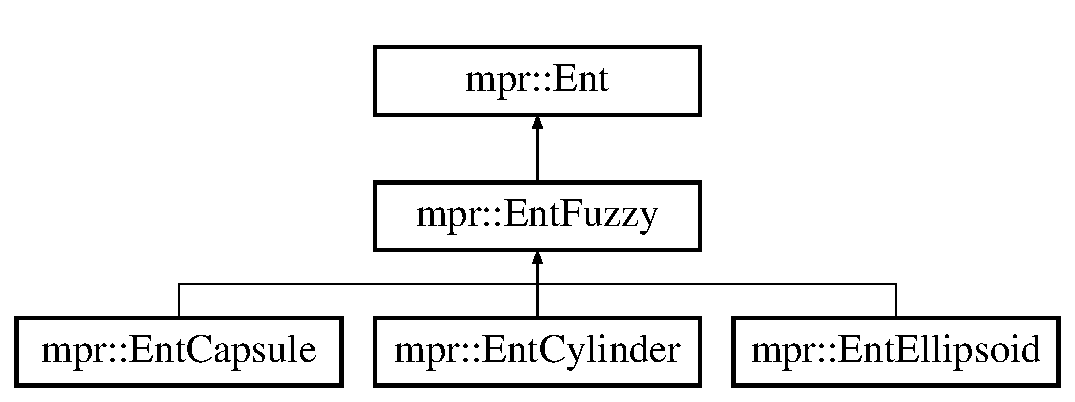
\includegraphics[height=3.000000cm]{structmpr_1_1_ent_fuzzy}
\end{center}
\end{figure}
\subsection*{Public Member Functions}
\begin{DoxyCompactItemize}
\item 
\mbox{\Hypertarget{structmpr_1_1_ent_fuzzy_adbacd7a821b7f9a66a1387b1d311e504}\label{structmpr_1_1_ent_fuzzy_adbacd7a821b7f9a66a1387b1d311e504}} 
{\bfseries Ent\+Fuzzy} (\hyperlink{structphysent}{physent} $\ast$ent)
\item 
\mbox{\Hypertarget{structmpr_1_1_ent_fuzzy_a98b9105fdc822a5e80c38a9cd0eb77d9}\label{structmpr_1_1_ent_fuzzy_a98b9105fdc822a5e80c38a9cd0eb77d9}} 
float {\bfseries left} () const
\item 
\mbox{\Hypertarget{structmpr_1_1_ent_fuzzy_a5878f71efa456acc0aec1e9e6c4535df}\label{structmpr_1_1_ent_fuzzy_a5878f71efa456acc0aec1e9e6c4535df}} 
float {\bfseries right} () const
\item 
\mbox{\Hypertarget{structmpr_1_1_ent_fuzzy_ab2b29319894c7687391e67ef816fb092}\label{structmpr_1_1_ent_fuzzy_ab2b29319894c7687391e67ef816fb092}} 
float {\bfseries back} () const
\item 
\mbox{\Hypertarget{structmpr_1_1_ent_fuzzy_a0ffdd59c9159ab3dde3ab2095c173d7a}\label{structmpr_1_1_ent_fuzzy_a0ffdd59c9159ab3dde3ab2095c173d7a}} 
float {\bfseries front} () const
\item 
\mbox{\Hypertarget{structmpr_1_1_ent_fuzzy_a9ae63300abca95f4d0b470594551ab83}\label{structmpr_1_1_ent_fuzzy_a9ae63300abca95f4d0b470594551ab83}} 
float {\bfseries bottom} () const
\item 
\mbox{\Hypertarget{structmpr_1_1_ent_fuzzy_aa5397d1e9f657b0526a8254715b03675}\label{structmpr_1_1_ent_fuzzy_aa5397d1e9f657b0526a8254715b03675}} 
float {\bfseries top} () const
\end{DoxyCompactItemize}
\subsection*{Additional Inherited Members}


The documentation for this struct was generated from the following file\+:\begin{DoxyCompactItemize}
\item 
H\+:/\+Rival\+Engine/\+Rival\+\_\+\+Game\+\_\+\+Engine\+\_\+\+G\+I\+T/\+Rival3dengine/source/engine/mpr.\+h\end{DoxyCompactItemize}

\hypertarget{structentity}{}\section{entity Struct Reference}
\label{structentity}\index{entity@{entity}}
Inheritance diagram for entity\+:\begin{figure}[H]
\begin{center}
\leavevmode
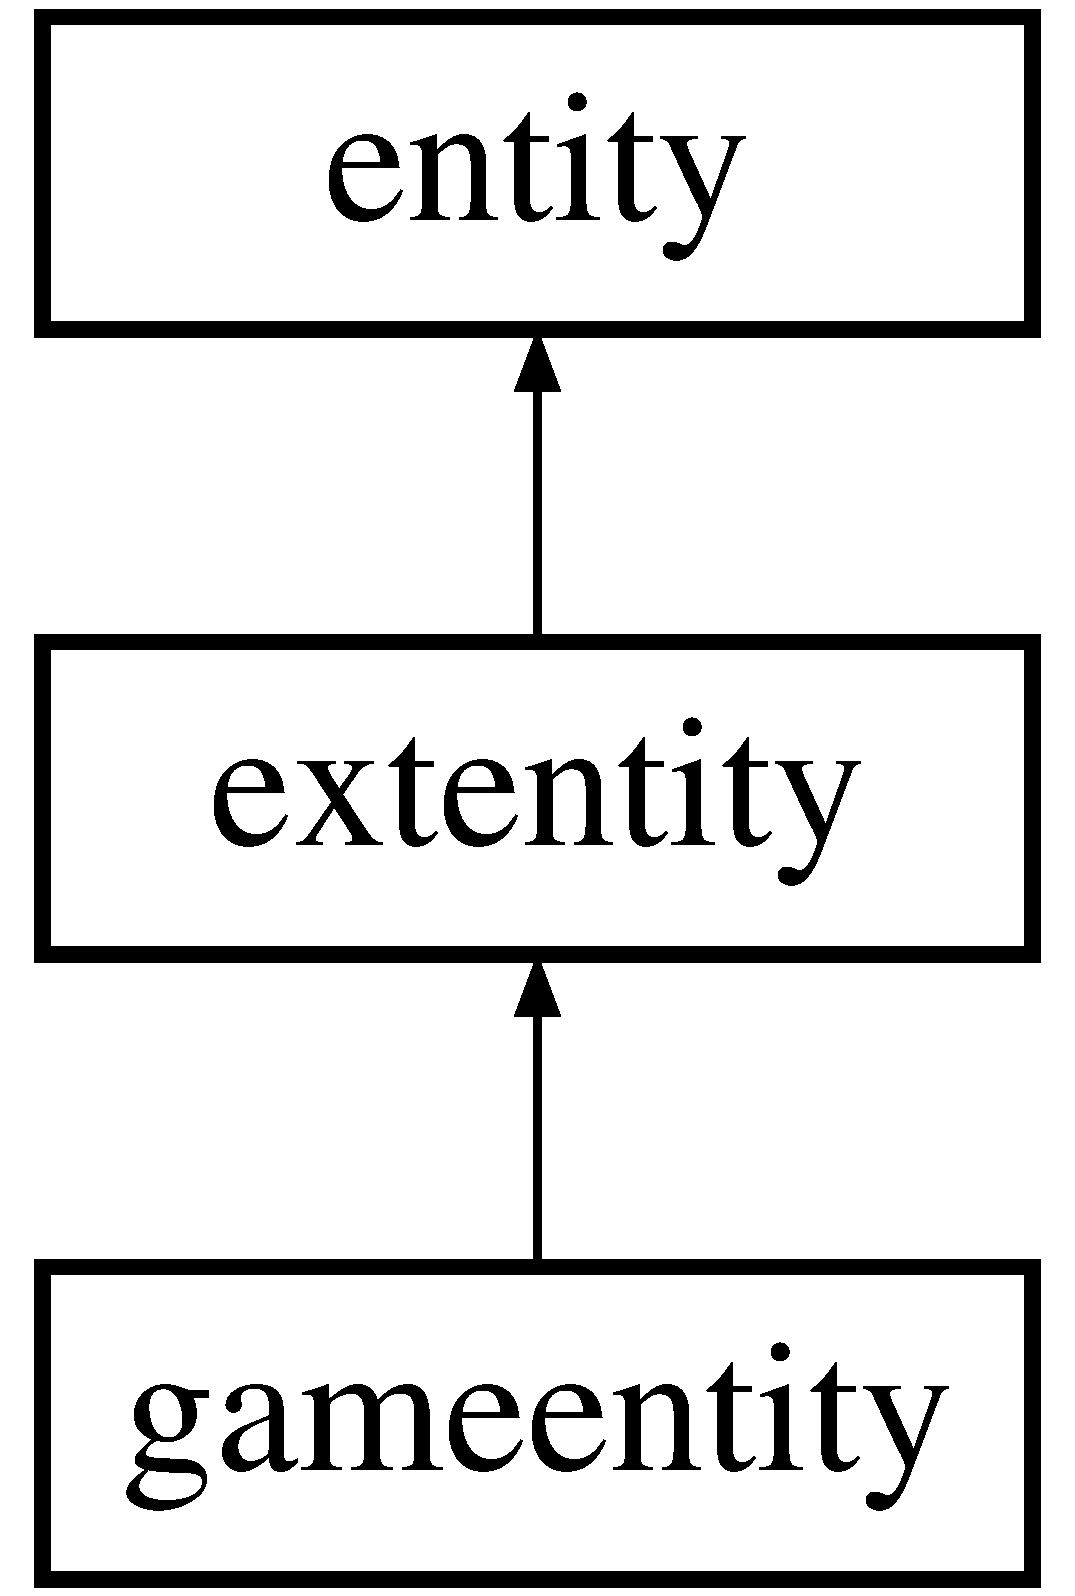
\includegraphics[height=3.000000cm]{structentity}
\end{center}
\end{figure}
\subsection*{Public Attributes}
\begin{DoxyCompactItemize}
\item 
\mbox{\Hypertarget{structentity_a525c90c5512cbb504f7ac9ab7014336f}\label{structentity_a525c90c5512cbb504f7ac9ab7014336f}} 
\hyperlink{structvec}{vec} {\bfseries o}
\item 
\mbox{\Hypertarget{structentity_a0906ab7e340820c4207da45e572c0525}\label{structentity_a0906ab7e340820c4207da45e572c0525}} 
short {\bfseries attr1}
\item 
\mbox{\Hypertarget{structentity_aadcc9c36f34cd97cb9104dfcba3837e1}\label{structentity_aadcc9c36f34cd97cb9104dfcba3837e1}} 
short {\bfseries attr2}
\item 
\mbox{\Hypertarget{structentity_a84d04e109e32479542f0495fdc30c2e3}\label{structentity_a84d04e109e32479542f0495fdc30c2e3}} 
short {\bfseries attr3}
\item 
\mbox{\Hypertarget{structentity_a33825bffeac8465cdeb6a6e37fa460c6}\label{structentity_a33825bffeac8465cdeb6a6e37fa460c6}} 
short {\bfseries attr4}
\item 
\mbox{\Hypertarget{structentity_a70fab3b3b43a8fa51e997d7b13d74dac}\label{structentity_a70fab3b3b43a8fa51e997d7b13d74dac}} 
short {\bfseries attr5}
\item 
\mbox{\Hypertarget{structentity_a8149790bddae92665ede0d60432f2dee}\label{structentity_a8149790bddae92665ede0d60432f2dee}} 
uchar {\bfseries type}
\item 
\mbox{\Hypertarget{structentity_af1b78967a757632a36536216c3ec9269}\label{structentity_af1b78967a757632a36536216c3ec9269}} 
uchar {\bfseries reserved}
\end{DoxyCompactItemize}


The documentation for this struct was generated from the following file\+:\begin{DoxyCompactItemize}
\item 
H\+:/\+Rival\+Engine/\+Rival\+\_\+\+Game\+\_\+\+Engine\+\_\+\+G\+I\+T/\+Rival3dengine/source/shared/ents.\+h\end{DoxyCompactItemize}

\hypertarget{structmpr_1_1_ent_o_b_b}{}\section{mpr\+:\+:Ent\+O\+BB Struct Reference}
\label{structmpr_1_1_ent_o_b_b}\index{mpr\+::\+Ent\+O\+BB@{mpr\+::\+Ent\+O\+BB}}
Inheritance diagram for mpr\+:\+:Ent\+O\+BB\+:\begin{figure}[H]
\begin{center}
\leavevmode
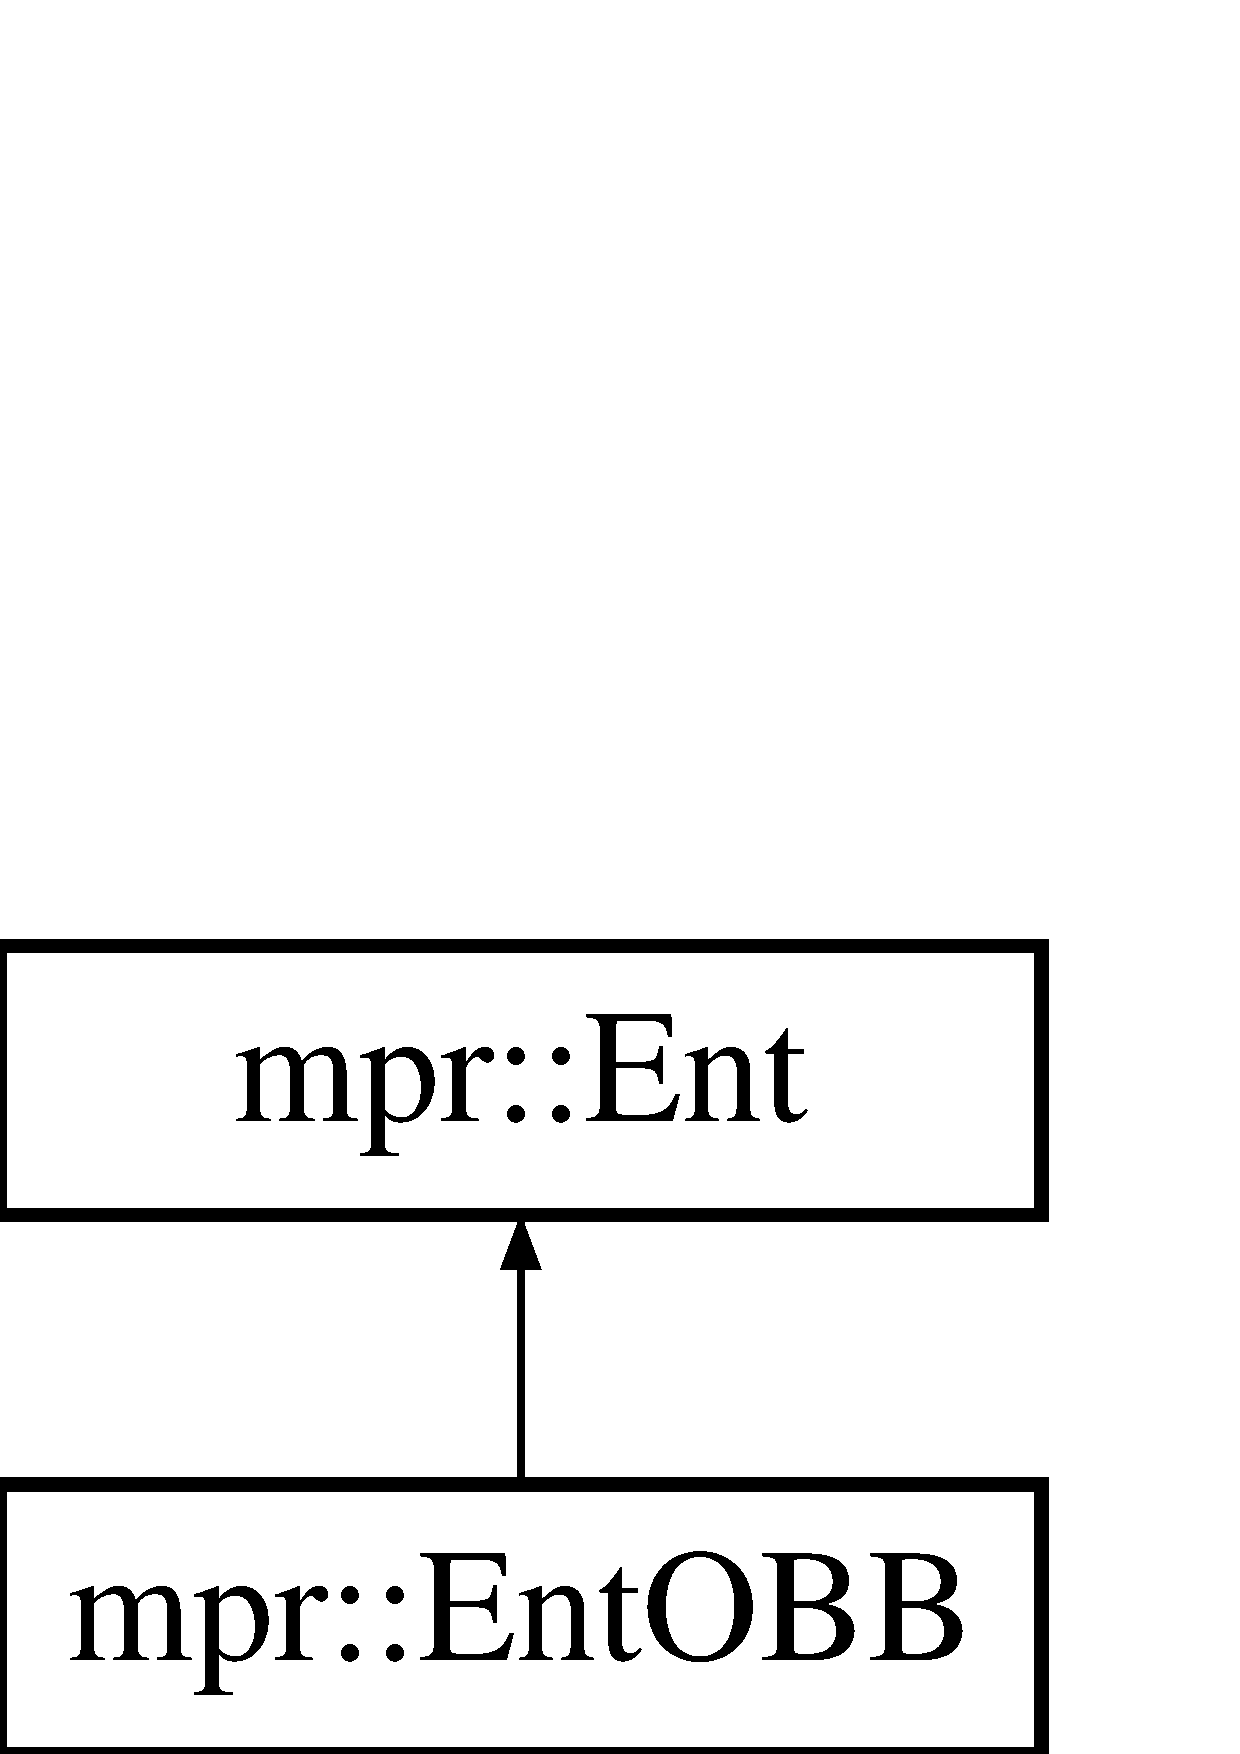
\includegraphics[height=2.000000cm]{structmpr_1_1_ent_o_b_b}
\end{center}
\end{figure}
\subsection*{Public Member Functions}
\begin{DoxyCompactItemize}
\item 
\mbox{\Hypertarget{structmpr_1_1_ent_o_b_b_aed2893ddefe67a255f5a26e8b3d86028}\label{structmpr_1_1_ent_o_b_b_aed2893ddefe67a255f5a26e8b3d86028}} 
{\bfseries Ent\+O\+BB} (\hyperlink{structphysent}{physent} $\ast$ent, float zmargin=0)
\item 
\mbox{\Hypertarget{structmpr_1_1_ent_o_b_b_ac86bbb813403c6e159b6fd7da871657d}\label{structmpr_1_1_ent_o_b_b_ac86bbb813403c6e159b6fd7da871657d}} 
\hyperlink{structvec}{vec} {\bfseries center} () const
\item 
\mbox{\Hypertarget{structmpr_1_1_ent_o_b_b_a4ae856b7375a46fd9d9ad1a5343f5129}\label{structmpr_1_1_ent_o_b_b_a4ae856b7375a46fd9d9ad1a5343f5129}} 
\hyperlink{structvec}{vec} {\bfseries contactface} (const \hyperlink{structvec}{vec} \&wn, const \hyperlink{structvec}{vec} \&wdir) const
\item 
\mbox{\Hypertarget{structmpr_1_1_ent_o_b_b_aa99c23096cf193cfbb948692374e471f}\label{structmpr_1_1_ent_o_b_b_aa99c23096cf193cfbb948692374e471f}} 
\hyperlink{structvec}{vec} {\bfseries localsupportpoint} (const \hyperlink{structvec}{vec} \&ln) const
\item 
\mbox{\Hypertarget{structmpr_1_1_ent_o_b_b_a7cf0951be22d8575c1ce31d128277da6}\label{structmpr_1_1_ent_o_b_b_a7cf0951be22d8575c1ce31d128277da6}} 
\hyperlink{structvec}{vec} {\bfseries supportpoint} (const \hyperlink{structvec}{vec} \&n) const
\item 
\mbox{\Hypertarget{structmpr_1_1_ent_o_b_b_a5c4903b931c11da7508139cbf37d44a3}\label{structmpr_1_1_ent_o_b_b_a5c4903b931c11da7508139cbf37d44a3}} 
float {\bfseries supportcoordneg} (const \hyperlink{structvec}{vec} \&p) const
\item 
\mbox{\Hypertarget{structmpr_1_1_ent_o_b_b_a0afb00399c16cc28505819f97a7d297f}\label{structmpr_1_1_ent_o_b_b_a0afb00399c16cc28505819f97a7d297f}} 
float {\bfseries supportcoord} (const \hyperlink{structvec}{vec} \&p) const
\item 
\mbox{\Hypertarget{structmpr_1_1_ent_o_b_b_ab0e912a5d16f063eabcf99138810c6cb}\label{structmpr_1_1_ent_o_b_b_ab0e912a5d16f063eabcf99138810c6cb}} 
float {\bfseries left} () const
\item 
\mbox{\Hypertarget{structmpr_1_1_ent_o_b_b_a66d8f4e1d6ca76960be391060d7383e7}\label{structmpr_1_1_ent_o_b_b_a66d8f4e1d6ca76960be391060d7383e7}} 
float {\bfseries right} () const
\item 
\mbox{\Hypertarget{structmpr_1_1_ent_o_b_b_a92d949210b611322d123eefa79374d06}\label{structmpr_1_1_ent_o_b_b_a92d949210b611322d123eefa79374d06}} 
float {\bfseries back} () const
\item 
\mbox{\Hypertarget{structmpr_1_1_ent_o_b_b_a7b135a593d7f443cfb5b77731a9d276e}\label{structmpr_1_1_ent_o_b_b_a7b135a593d7f443cfb5b77731a9d276e}} 
float {\bfseries front} () const
\item 
\mbox{\Hypertarget{structmpr_1_1_ent_o_b_b_adb4723b4da461924e9d1c9f0c92046b8}\label{structmpr_1_1_ent_o_b_b_adb4723b4da461924e9d1c9f0c92046b8}} 
float {\bfseries bottom} () const
\item 
\mbox{\Hypertarget{structmpr_1_1_ent_o_b_b_ad55d7e8d7082890fa0e75cbbe5692464}\label{structmpr_1_1_ent_o_b_b_ad55d7e8d7082890fa0e75cbbe5692464}} 
float {\bfseries top} () const
\end{DoxyCompactItemize}
\subsection*{Public Attributes}
\begin{DoxyCompactItemize}
\item 
\mbox{\Hypertarget{structmpr_1_1_ent_o_b_b_aa1bbdce563c10adcbc1baedf2c91ea31}\label{structmpr_1_1_ent_o_b_b_aa1bbdce563c10adcbc1baedf2c91ea31}} 
\hyperlink{structmatrix3}{matrix3} {\bfseries orient}
\item 
\mbox{\Hypertarget{structmpr_1_1_ent_o_b_b_aa8ef9994738587f90de7ceaf0a09561a}\label{structmpr_1_1_ent_o_b_b_aa8ef9994738587f90de7ceaf0a09561a}} 
float {\bfseries zmargin}
\end{DoxyCompactItemize}


The documentation for this struct was generated from the following file\+:\begin{DoxyCompactItemize}
\item 
H\+:/\+Rival\+Engine/\+Rival\+\_\+\+Game\+\_\+\+Engine\+\_\+\+G\+I\+T/\+Rival3dengine/source/engine/mpr.\+h\end{DoxyCompactItemize}

\hypertarget{structenvmap}{}\section{envmap Struct Reference}
\label{structenvmap}\index{envmap@{envmap}}
\subsection*{Public Member Functions}
\begin{DoxyCompactItemize}
\item 
\mbox{\Hypertarget{structenvmap_a33710258484f4def80c3e4e118f180d4}\label{structenvmap_a33710258484f4def80c3e4e118f180d4}} 
void {\bfseries clear} ()
\end{DoxyCompactItemize}
\subsection*{Public Attributes}
\begin{DoxyCompactItemize}
\item 
\mbox{\Hypertarget{structenvmap_ad09512d44815d54a48a3d121a9452367}\label{structenvmap_ad09512d44815d54a48a3d121a9452367}} 
int {\bfseries radius}
\item 
\mbox{\Hypertarget{structenvmap_a8477e381c937c54b52e53029f1082878}\label{structenvmap_a8477e381c937c54b52e53029f1082878}} 
int {\bfseries size}
\item 
\mbox{\Hypertarget{structenvmap_a61a4748a1a96822c51c5c6142f7c7792}\label{structenvmap_a61a4748a1a96822c51c5c6142f7c7792}} 
int {\bfseries blur}
\item 
\mbox{\Hypertarget{structenvmap_a652614f98da0ecda8764c55b33c19709}\label{structenvmap_a652614f98da0ecda8764c55b33c19709}} 
\hyperlink{structvec}{vec} {\bfseries o}
\item 
\mbox{\Hypertarget{structenvmap_a3cfad0c28f680d4aa113ab74a21b15cb}\label{structenvmap_a3cfad0c28f680d4aa113ab74a21b15cb}} 
G\+Luint {\bfseries tex}
\end{DoxyCompactItemize}


The documentation for this struct was generated from the following file\+:\begin{DoxyCompactItemize}
\item 
H\+:/\+Rival\+Engine/\+Rival\+\_\+\+Game\+\_\+\+Engine\+\_\+\+G\+I\+T/\+Rival3dengine/source/engine/texture.\+cpp\end{DoxyCompactItemize}

\hypertarget{structserver_1_1explodeevent}{}\section{server\+:\+:explodeevent Struct Reference}
\label{structserver_1_1explodeevent}\index{server\+::explodeevent@{server\+::explodeevent}}
Inheritance diagram for server\+:\+:explodeevent\+:\begin{figure}[H]
\begin{center}
\leavevmode
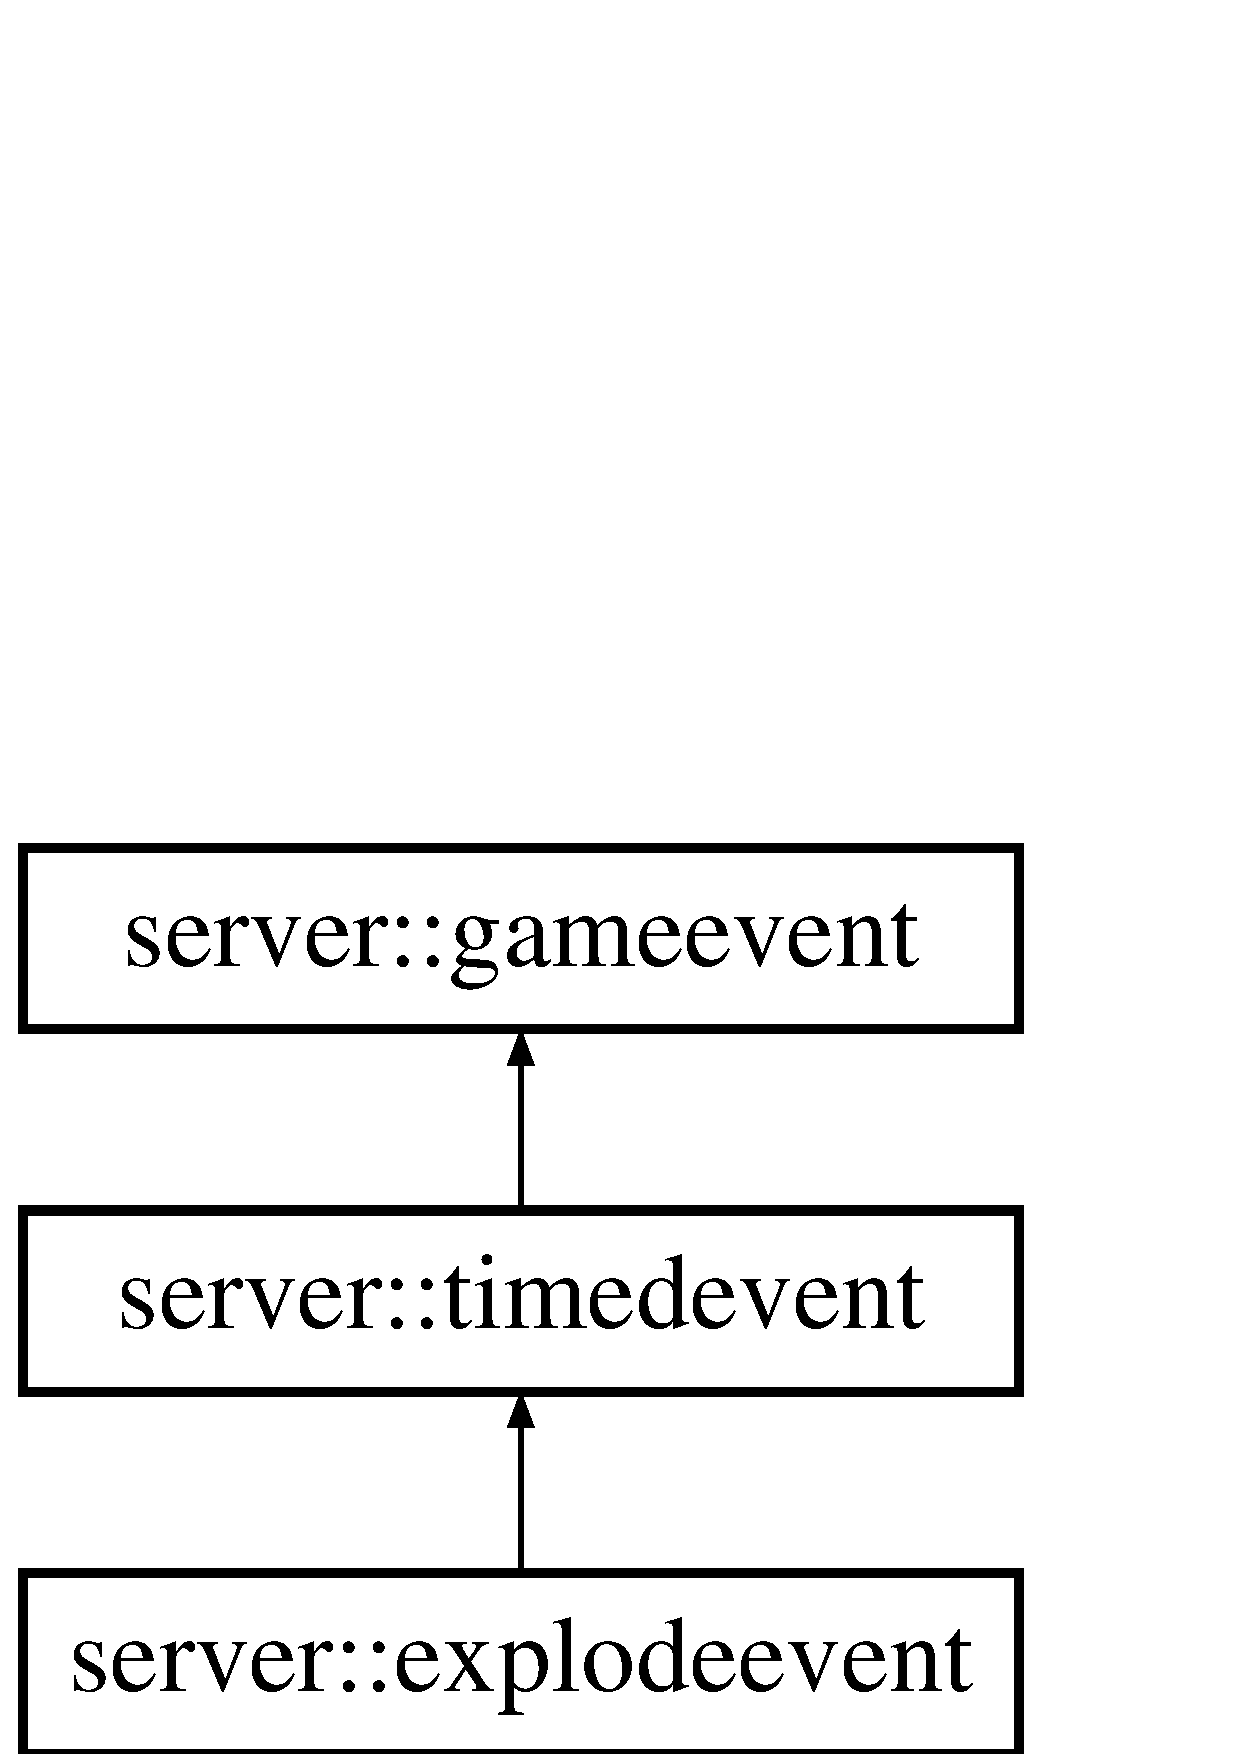
\includegraphics[height=3.000000cm]{structserver_1_1explodeevent}
\end{center}
\end{figure}
\subsection*{Public Member Functions}
\begin{DoxyCompactItemize}
\item 
\mbox{\Hypertarget{structserver_1_1explodeevent_a922533d747254b4de7e1bb0b835093e6}\label{structserver_1_1explodeevent_a922533d747254b4de7e1bb0b835093e6}} 
bool {\bfseries keepable} () const
\item 
\mbox{\Hypertarget{structserver_1_1explodeevent_a2fa3c77ed6ca7f9d533f3c0608ab7d72}\label{structserver_1_1explodeevent_a2fa3c77ed6ca7f9d533f3c0608ab7d72}} 
void {\bfseries process} (\hyperlink{structserver_1_1clientinfo}{clientinfo} $\ast$ci)
\end{DoxyCompactItemize}
\subsection*{Public Attributes}
\begin{DoxyCompactItemize}
\item 
\mbox{\Hypertarget{structserver_1_1explodeevent_aeb8122d0793e67712d7568a427f54b66}\label{structserver_1_1explodeevent_aeb8122d0793e67712d7568a427f54b66}} 
int {\bfseries id}
\item 
\mbox{\Hypertarget{structserver_1_1explodeevent_adbc194a0a3eb9d32d2267b48cbc98663}\label{structserver_1_1explodeevent_adbc194a0a3eb9d32d2267b48cbc98663}} 
int {\bfseries atk}
\item 
\mbox{\Hypertarget{structserver_1_1explodeevent_a405e8e162bd75305faf9102d52def51e}\label{structserver_1_1explodeevent_a405e8e162bd75305faf9102d52def51e}} 
\hyperlink{structvector}{vector}$<$ \hyperlink{structserver_1_1hitinfo}{hitinfo} $>$ {\bfseries hits}
\end{DoxyCompactItemize}


The documentation for this struct was generated from the following file\+:\begin{DoxyCompactItemize}
\item 
H\+:/\+Rival\+Engine/\+Rival\+\_\+\+Game\+\_\+\+Engine\+\_\+\+G\+I\+T/\+Rival3dengine/source/game/server.\+cpp\end{DoxyCompactItemize}

\hypertarget{structextentity}{}\section{extentity Struct Reference}
\label{structextentity}\index{extentity@{extentity}}
Inheritance diagram for extentity\+:\begin{figure}[H]
\begin{center}
\leavevmode
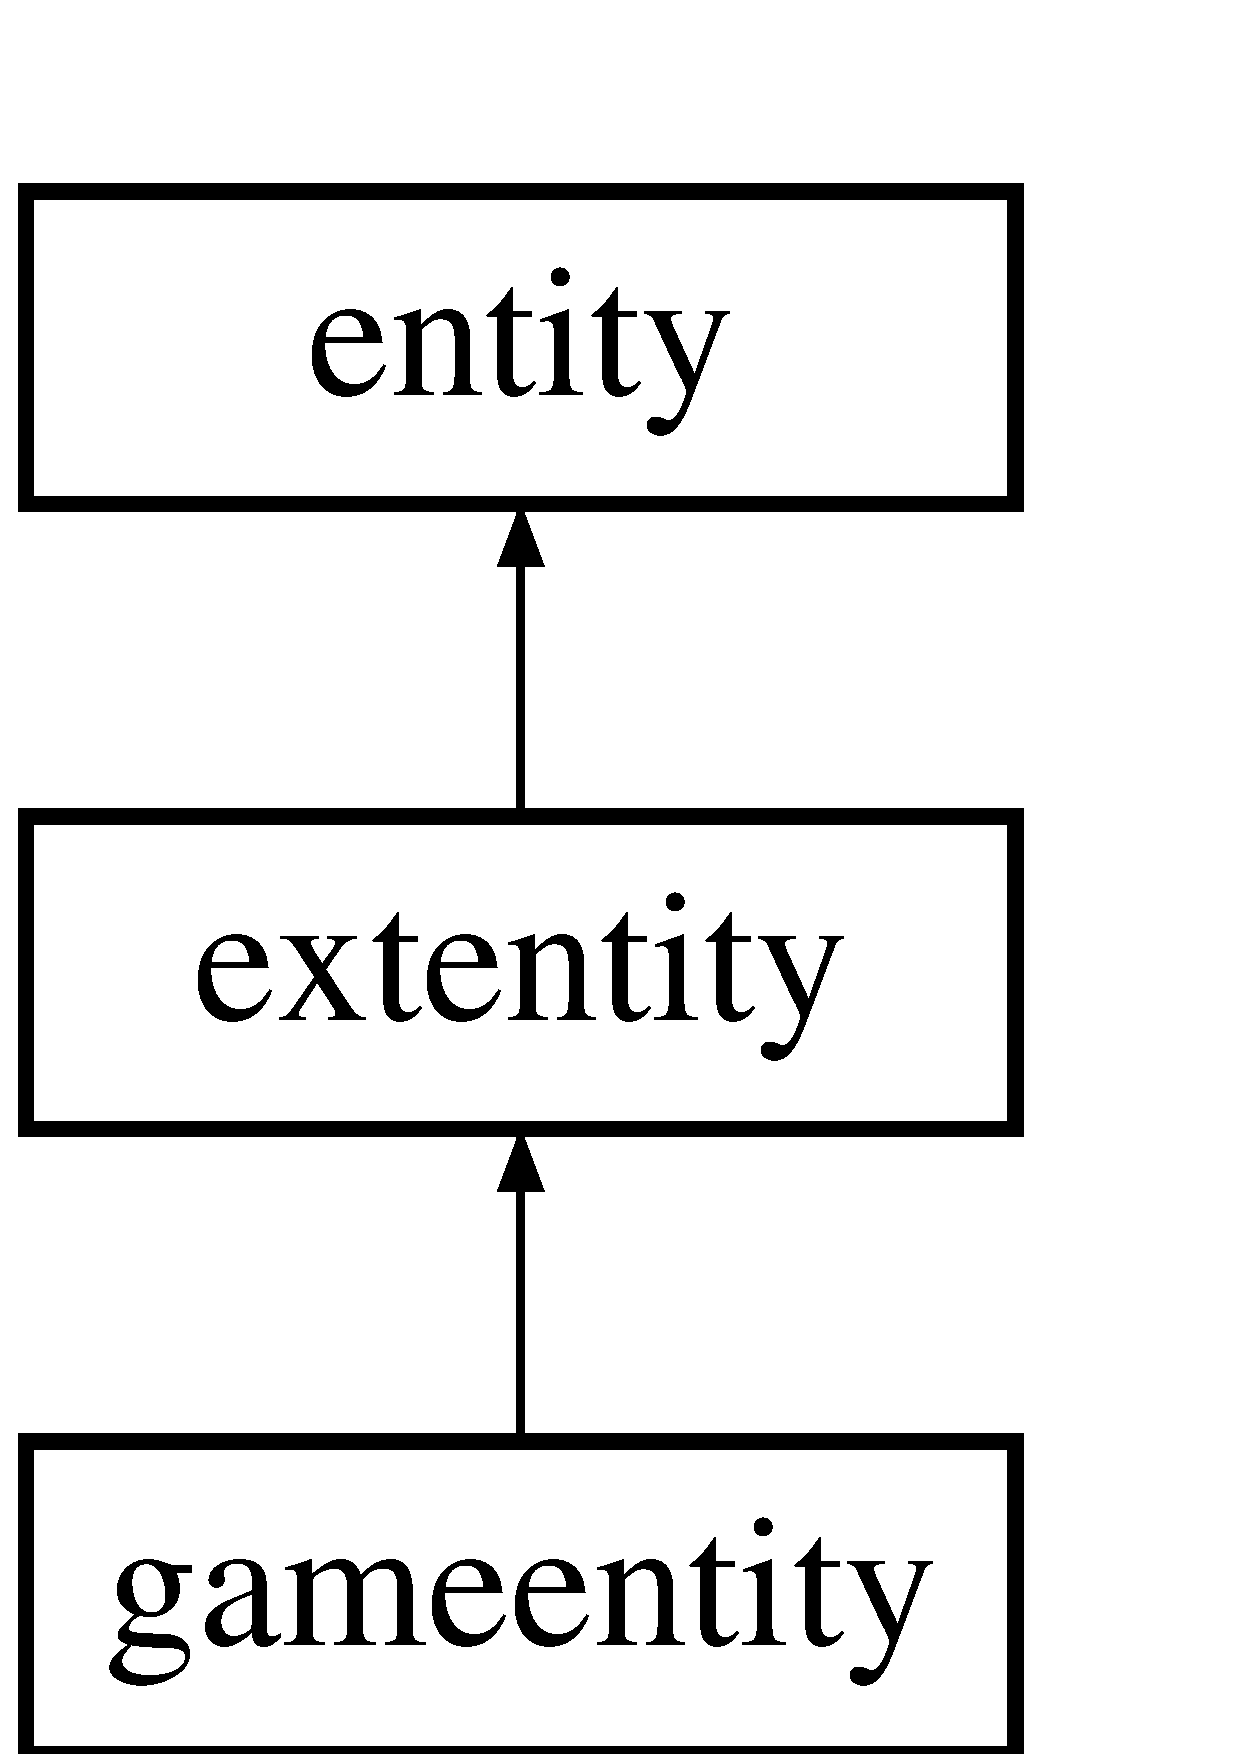
\includegraphics[height=3.000000cm]{structextentity}
\end{center}
\end{figure}
\subsection*{Public Member Functions}
\begin{DoxyCompactItemize}
\item 
\mbox{\Hypertarget{structextentity_a7e4a1c4198c82649ce166fa6045bf459}\label{structextentity_a7e4a1c4198c82649ce166fa6045bf459}} 
bool {\bfseries spawned} () const
\item 
\mbox{\Hypertarget{structextentity_aa48299a46ca4dad1e7061dfd67d2a967}\label{structextentity_aa48299a46ca4dad1e7061dfd67d2a967}} 
void {\bfseries setspawned} (bool val)
\item 
\mbox{\Hypertarget{structextentity_ab0fe8f61de631195dd3c1134a332359a}\label{structextentity_ab0fe8f61de631195dd3c1134a332359a}} 
void {\bfseries setspawned} ()
\item 
\mbox{\Hypertarget{structextentity_ae4758bde8de9292792a298f2fea11963}\label{structextentity_ae4758bde8de9292792a298f2fea11963}} 
void {\bfseries clearspawned} ()
\end{DoxyCompactItemize}
\subsection*{Public Attributes}
\begin{DoxyCompactItemize}
\item 
\mbox{\Hypertarget{structextentity_a7a6c7b585d672811eae4870b730d8cf2}\label{structextentity_a7a6c7b585d672811eae4870b730d8cf2}} 
int {\bfseries flags}
\item 
\mbox{\Hypertarget{structextentity_aa0fd6e32aba51def1b455b69a4bc9be4}\label{structextentity_aa0fd6e32aba51def1b455b69a4bc9be4}} 
\hyperlink{structextentity}{extentity} $\ast$ {\bfseries attached}
\end{DoxyCompactItemize}


The documentation for this struct was generated from the following file\+:\begin{DoxyCompactItemize}
\item 
H\+:/\+Rival\+Engine/\+Rival\+\_\+\+Game\+\_\+\+Engine\+\_\+\+G\+I\+T/\+Rival3dengine/source/shared/ents.\+h\end{DoxyCompactItemize}

\hypertarget{structfacebounds}{}\section{facebounds Struct Reference}
\label{structfacebounds}\index{facebounds@{facebounds}}
\subsection*{Public Member Functions}
\begin{DoxyCompactItemize}
\item 
\mbox{\Hypertarget{structfacebounds_a2559fdb02a2c7d95a2a8b41bc371da9b}\label{structfacebounds_a2559fdb02a2c7d95a2a8b41bc371da9b}} 
bool {\bfseries empty} () const
\end{DoxyCompactItemize}
\subsection*{Public Attributes}
\begin{DoxyCompactItemize}
\item 
\mbox{\Hypertarget{structfacebounds_a2822bc508bbd5c2faedbdb80454189c9}\label{structfacebounds_a2822bc508bbd5c2faedbdb80454189c9}} 
ushort {\bfseries u1}
\item 
\mbox{\Hypertarget{structfacebounds_a8d7a70867d20717aac1837e6526bda5b}\label{structfacebounds_a8d7a70867d20717aac1837e6526bda5b}} 
ushort {\bfseries u2}
\item 
\mbox{\Hypertarget{structfacebounds_af351c284ab1d1c9058b85e1ebcbad0a6}\label{structfacebounds_af351c284ab1d1c9058b85e1ebcbad0a6}} 
ushort {\bfseries v1}
\item 
\mbox{\Hypertarget{structfacebounds_af927adeeadafdf15bd17c3e298b24a3f}\label{structfacebounds_af927adeeadafdf15bd17c3e298b24a3f}} 
ushort {\bfseries v2}
\end{DoxyCompactItemize}


The documentation for this struct was generated from the following file\+:\begin{DoxyCompactItemize}
\item 
H\+:/\+Rival\+Engine/\+Rival\+\_\+\+Game\+\_\+\+Engine\+\_\+\+G\+I\+T/\+Rival3dengine/source/engine/octa.\+h\end{DoxyCompactItemize}

\hypertarget{struct_u_i_1_1_field}{}\section{UI\+:\+:Field Struct Reference}
\label{struct_u_i_1_1_field}\index{U\+I\+::\+Field@{U\+I\+::\+Field}}
Inheritance diagram for UI\+:\+:Field\+:\begin{figure}[H]
\begin{center}
\leavevmode
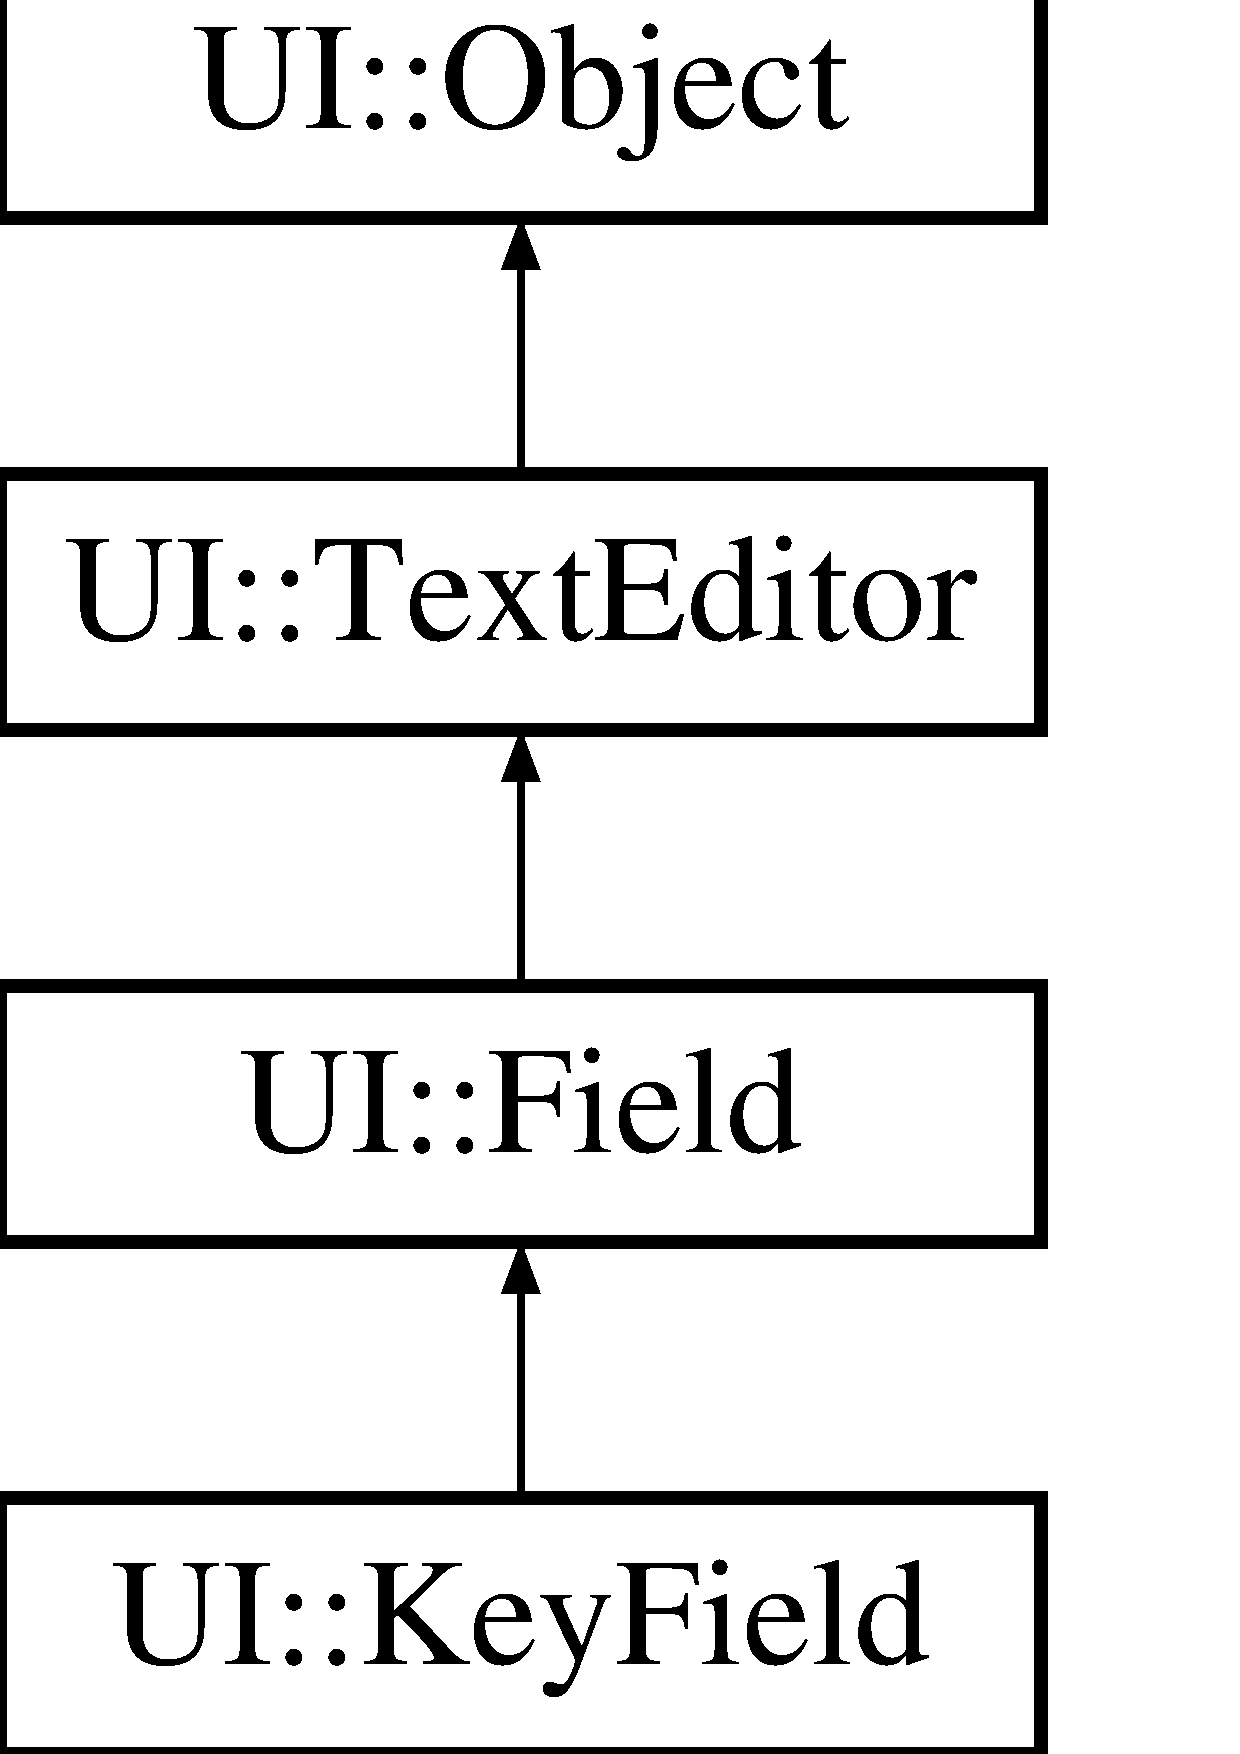
\includegraphics[height=4.000000cm]{struct_u_i_1_1_field}
\end{center}
\end{figure}
\subsection*{Public Member Functions}
\begin{DoxyCompactItemize}
\item 
\mbox{\Hypertarget{struct_u_i_1_1_field_ab43dc0e4ad5f9764af01c27467db87c0}\label{struct_u_i_1_1_field_ab43dc0e4ad5f9764af01c27467db87c0}} 
void {\bfseries setup} (\hyperlink{structident}{ident} $\ast$id\+\_\+, int length, uint $\ast$onchange, float scale=1, const char $\ast$keyfilter\+\_\+=N\+U\+LL)
\item 
\mbox{\Hypertarget{struct_u_i_1_1_field_a590b3f0cdfa1d4040dde2b9c65777e37}\label{struct_u_i_1_1_field_a590b3f0cdfa1d4040dde2b9c65777e37}} 
const char $\ast$ {\bfseries gettype} () const
\item 
\mbox{\Hypertarget{struct_u_i_1_1_field_a34b63e1013d2050c92dc8a5049325cb6}\label{struct_u_i_1_1_field_a34b63e1013d2050c92dc8a5049325cb6}} 
void {\bfseries commit} ()
\item 
\mbox{\Hypertarget{struct_u_i_1_1_field_a47c63127b38f926f8079ca021e226077}\label{struct_u_i_1_1_field_a47c63127b38f926f8079ca021e226077}} 
void {\bfseries cancel} ()
\end{DoxyCompactItemize}
\subsection*{Static Public Member Functions}
\begin{DoxyCompactItemize}
\item 
\mbox{\Hypertarget{struct_u_i_1_1_field_a74b316511cafe0855e8daeaae6cfbfda}\label{struct_u_i_1_1_field_a74b316511cafe0855e8daeaae6cfbfda}} 
static const char $\ast$ {\bfseries typestr} ()
\end{DoxyCompactItemize}
\subsection*{Public Attributes}
\begin{DoxyCompactItemize}
\item 
\mbox{\Hypertarget{struct_u_i_1_1_field_a1a5b197297f9079eb7b722ec3bf25b0a}\label{struct_u_i_1_1_field_a1a5b197297f9079eb7b722ec3bf25b0a}} 
\hyperlink{structident}{ident} $\ast$ {\bfseries id}
\item 
\mbox{\Hypertarget{struct_u_i_1_1_field_a204f89f324bb5ba87a539f784657e092}\label{struct_u_i_1_1_field_a204f89f324bb5ba87a539f784657e092}} 
bool {\bfseries changed}
\end{DoxyCompactItemize}
\subsection*{Additional Inherited Members}


The documentation for this struct was generated from the following file\+:\begin{DoxyCompactItemize}
\item 
H\+:/\+Rival\+Engine/\+Rival\+\_\+\+Game\+\_\+\+Engine\+\_\+\+G\+I\+T/\+Rival3dengine/source/engine/ui.\+cpp\end{DoxyCompactItemize}

\hypertarget{structfileskey}{}\section{fileskey Struct Reference}
\label{structfileskey}\index{fileskey@{fileskey}}
\subsection*{Public Member Functions}
\begin{DoxyCompactItemize}
\item 
\mbox{\Hypertarget{structfileskey_a7c397022d00a7bd1402e8398f88ea31a}\label{structfileskey_a7c397022d00a7bd1402e8398f88ea31a}} 
{\bfseries fileskey} (int type, const char $\ast$dir, const char $\ast$ext)
\end{DoxyCompactItemize}
\subsection*{Public Attributes}
\begin{DoxyCompactItemize}
\item 
\mbox{\Hypertarget{structfileskey_a238a30fb793973e0e8d5ba4e7a860f5b}\label{structfileskey_a238a30fb793973e0e8d5ba4e7a860f5b}} 
int {\bfseries type}
\item 
\mbox{\Hypertarget{structfileskey_ab05a6fdd16c979a90faa229fe603b771}\label{structfileskey_ab05a6fdd16c979a90faa229fe603b771}} 
const char $\ast$ {\bfseries dir}
\item 
\mbox{\Hypertarget{structfileskey_ab2e3d6cf43c8511de829e88bb65e7a1d}\label{structfileskey_ab2e3d6cf43c8511de829e88bb65e7a1d}} 
const char $\ast$ {\bfseries ext}
\end{DoxyCompactItemize}


The documentation for this struct was generated from the following file\+:\begin{DoxyCompactItemize}
\item 
H\+:/\+Rival\+Engine/\+Rival\+\_\+\+Game\+\_\+\+Engine\+\_\+\+G\+I\+T/\+Rival3dengine/source/engine/console.\+cpp\end{DoxyCompactItemize}

\hypertarget{structfilestream}{}\section{filestream Struct Reference}
\label{structfilestream}\index{filestream@{filestream}}
Inheritance diagram for filestream\+:\begin{figure}[H]
\begin{center}
\leavevmode
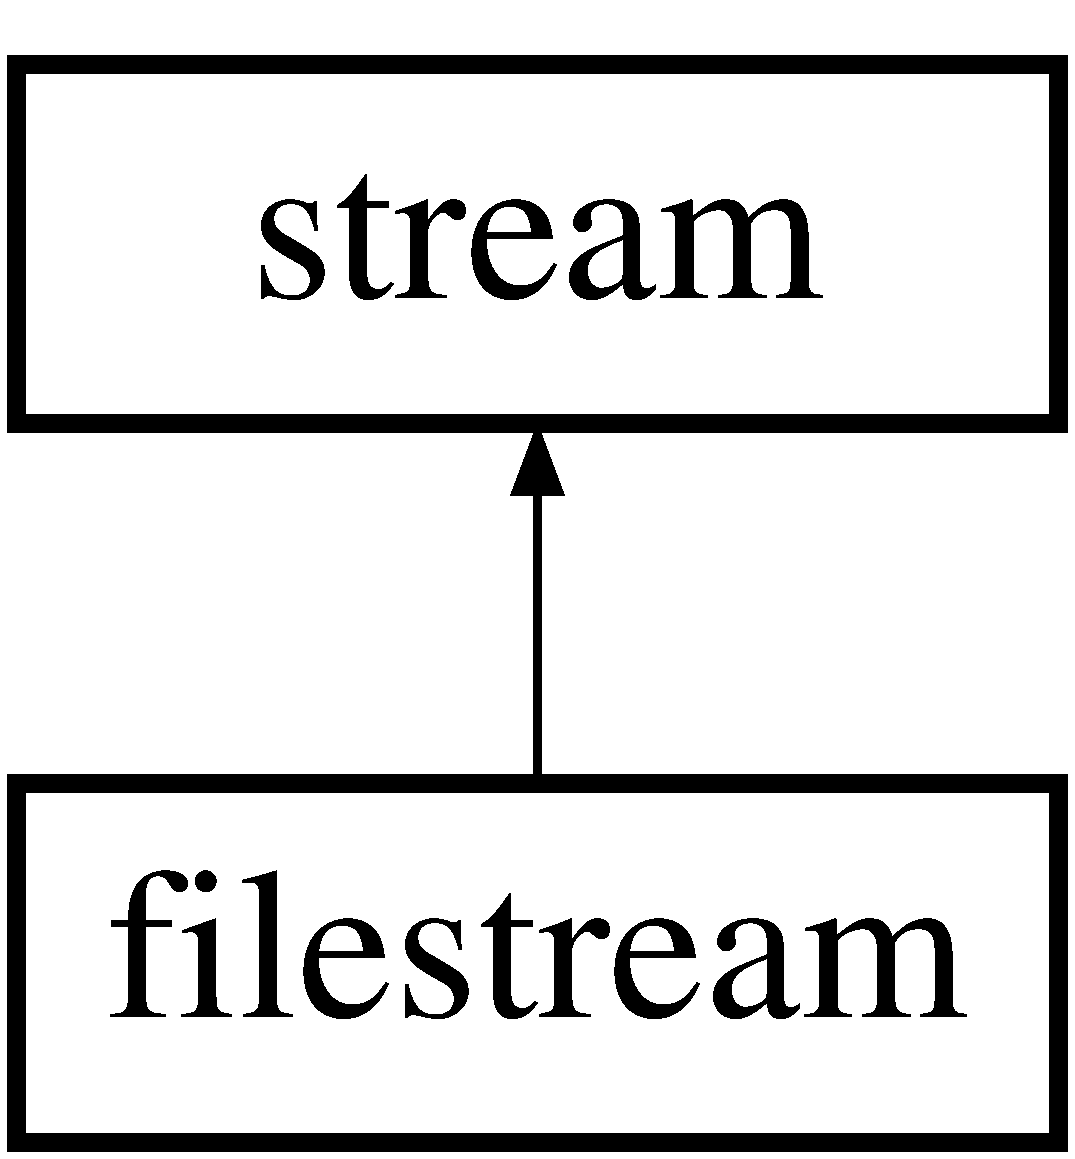
\includegraphics[height=2.000000cm]{structfilestream}
\end{center}
\end{figure}
\subsection*{Public Member Functions}
\begin{DoxyCompactItemize}
\item 
\mbox{\Hypertarget{structfilestream_a18c1c59809a3774a95727d8953565ae8}\label{structfilestream_a18c1c59809a3774a95727d8953565ae8}} 
bool {\bfseries open} (const char $\ast$name, const char $\ast$mode)
\item 
\mbox{\Hypertarget{structfilestream_a9a37bf4a3fd00013950005926c2ccfdf}\label{structfilestream_a9a37bf4a3fd00013950005926c2ccfdf}} 
bool {\bfseries opentemp} (const char $\ast$name, const char $\ast$mode)
\item 
\mbox{\Hypertarget{structfilestream_ac030b860055a2d12d59c2289369c3790}\label{structfilestream_ac030b860055a2d12d59c2289369c3790}} 
void {\bfseries close} ()
\item 
\mbox{\Hypertarget{structfilestream_a894051c3ef1f83f09f1ee4056fd59d1e}\label{structfilestream_a894051c3ef1f83f09f1ee4056fd59d1e}} 
bool {\bfseries end} ()
\item 
\mbox{\Hypertarget{structfilestream_a30343412639d00eba3c738791d2ee4c1}\label{structfilestream_a30343412639d00eba3c738791d2ee4c1}} 
offset {\bfseries tell} ()
\item 
\mbox{\Hypertarget{structfilestream_a29d1cb0d40f08d28bd2b0ca5ad183399}\label{structfilestream_a29d1cb0d40f08d28bd2b0ca5ad183399}} 
bool {\bfseries seek} (offset pos, int whence)
\item 
\mbox{\Hypertarget{structfilestream_ab716330fc2db84e71b94c1b48d4ae582}\label{structfilestream_ab716330fc2db84e71b94c1b48d4ae582}} 
size\+\_\+t {\bfseries read} (void $\ast$buf, size\+\_\+t len)
\item 
\mbox{\Hypertarget{structfilestream_ac85ef07dc763c61cd32d84ce240ce614}\label{structfilestream_ac85ef07dc763c61cd32d84ce240ce614}} 
size\+\_\+t {\bfseries write} (const void $\ast$buf, size\+\_\+t len)
\item 
\mbox{\Hypertarget{structfilestream_ab67368c92e2e3f183b711c9d6d71917d}\label{structfilestream_ab67368c92e2e3f183b711c9d6d71917d}} 
bool {\bfseries flush} ()
\item 
\mbox{\Hypertarget{structfilestream_a26df7bffcdea0440c1a9ca8706e24e2f}\label{structfilestream_a26df7bffcdea0440c1a9ca8706e24e2f}} 
int {\bfseries getchar} ()
\item 
\mbox{\Hypertarget{structfilestream_a59ce02b686f4d15f391a212d9c97e107}\label{structfilestream_a59ce02b686f4d15f391a212d9c97e107}} 
bool {\bfseries putchar} (int c)
\item 
\mbox{\Hypertarget{structfilestream_a8e4bff33ab483af9b0d4df89e97b430c}\label{structfilestream_a8e4bff33ab483af9b0d4df89e97b430c}} 
bool {\bfseries getline} (char $\ast$str, size\+\_\+t len)
\item 
\mbox{\Hypertarget{structfilestream_a3ee81c389171cf8df112ed55705f8812}\label{structfilestream_a3ee81c389171cf8df112ed55705f8812}} 
bool {\bfseries putstring} (const char $\ast$str)
\item 
\mbox{\Hypertarget{structfilestream_a5eb1166b6dffb71df3f8c9eaf95248e6}\label{structfilestream_a5eb1166b6dffb71df3f8c9eaf95248e6}} 
size\+\_\+t {\bfseries printf} (const char $\ast$fmt,...)
\end{DoxyCompactItemize}
\subsection*{Public Attributes}
\begin{DoxyCompactItemize}
\item 
\mbox{\Hypertarget{structfilestream_a86369859a949d0e73414195894ff0aa9}\label{structfilestream_a86369859a949d0e73414195894ff0aa9}} 
F\+I\+LE $\ast$ {\bfseries file}
\end{DoxyCompactItemize}
\subsection*{Additional Inherited Members}


The documentation for this struct was generated from the following file\+:\begin{DoxyCompactItemize}
\item 
H\+:/\+Rival\+Engine/\+Rival\+\_\+\+Game\+\_\+\+Engine\+\_\+\+G\+I\+T/\+Rival3dengine/source/shared/stream.\+cpp\end{DoxyCompactItemize}

\hypertarget{structfilesval}{}\section{filesval Struct Reference}
\label{structfilesval}\index{filesval@{filesval}}
\subsection*{Public Member Functions}
\begin{DoxyCompactItemize}
\item 
\mbox{\Hypertarget{structfilesval_a3608a268ddda5107b2c89b69fe22db15}\label{structfilesval_a3608a268ddda5107b2c89b69fe22db15}} 
{\bfseries filesval} (int type, const char $\ast$dir, const char $\ast$ext)
\item 
\mbox{\Hypertarget{structfilesval_a57f2725d4798e3b82d58fbabcf73b861}\label{structfilesval_a57f2725d4798e3b82d58fbabcf73b861}} 
void {\bfseries update} ()
\end{DoxyCompactItemize}
\subsection*{Public Attributes}
\begin{DoxyCompactItemize}
\item 
\mbox{\Hypertarget{structfilesval_ad29dc1cdb726d32c8f044356bd4729aa}\label{structfilesval_ad29dc1cdb726d32c8f044356bd4729aa}} 
int {\bfseries type}
\item 
\mbox{\Hypertarget{structfilesval_ab7666251a3e02d8998af92fe3724618f}\label{structfilesval_ab7666251a3e02d8998af92fe3724618f}} 
char $\ast$ {\bfseries dir}
\item 
\mbox{\Hypertarget{structfilesval_a50dad30e727231aaec4031b30cec43bf}\label{structfilesval_a50dad30e727231aaec4031b30cec43bf}} 
char $\ast$ {\bfseries ext}
\item 
\mbox{\Hypertarget{structfilesval_a6db4a4f76467c311e63c3536ae2909f6}\label{structfilesval_a6db4a4f76467c311e63c3536ae2909f6}} 
\hyperlink{structvector}{vector}$<$ char $\ast$ $>$ {\bfseries files}
\item 
\mbox{\Hypertarget{structfilesval_a9697721fe8b96856f46212dbbeec1d74}\label{structfilesval_a9697721fe8b96856f46212dbbeec1d74}} 
int {\bfseries millis}
\end{DoxyCompactItemize}


The documentation for this struct was generated from the following file\+:\begin{DoxyCompactItemize}
\item 
H\+:/\+Rival\+Engine/\+Rival\+\_\+\+Game\+\_\+\+Engine\+\_\+\+G\+I\+T/\+Rival3dengine/source/engine/console.\+cpp\end{DoxyCompactItemize}

\hypertarget{struct_u_i_1_1_fill_color}{}\section{UI\+:\+:Fill\+Color Struct Reference}
\label{struct_u_i_1_1_fill_color}\index{U\+I\+::\+Fill\+Color@{U\+I\+::\+Fill\+Color}}
Inheritance diagram for UI\+:\+:Fill\+Color\+:\begin{figure}[H]
\begin{center}
\leavevmode
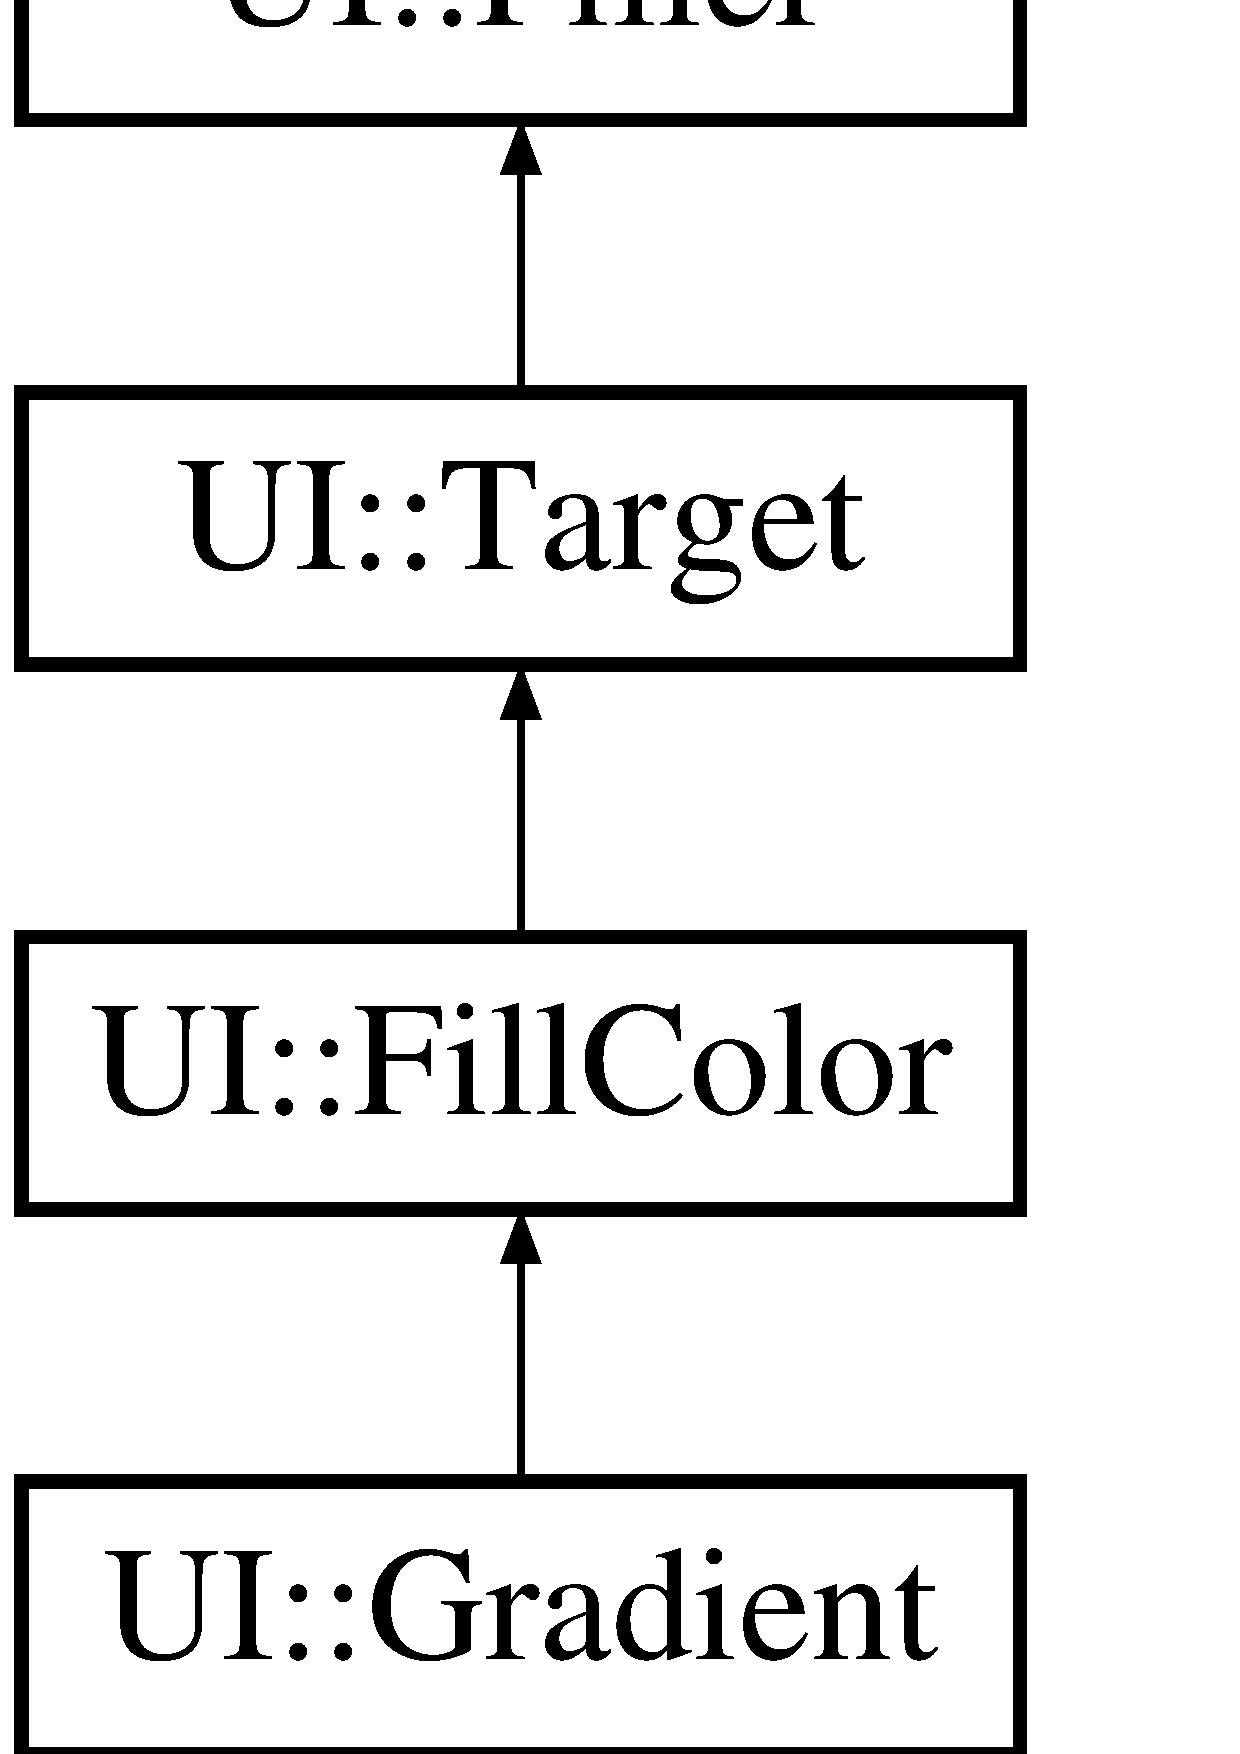
\includegraphics[height=5.000000cm]{struct_u_i_1_1_fill_color}
\end{center}
\end{figure}
\subsection*{Public Types}
\begin{DoxyCompactItemize}
\item 
\mbox{\Hypertarget{struct_u_i_1_1_fill_color_a99546f7ba25a5e08d61dfd0947b18770}\label{struct_u_i_1_1_fill_color_a99546f7ba25a5e08d61dfd0947b18770}} 
enum \{ {\bfseries S\+O\+L\+ID} = 0, 
{\bfseries M\+O\+D\+U\+L\+A\+TE}
 \}
\end{DoxyCompactItemize}
\subsection*{Public Member Functions}
\begin{DoxyCompactItemize}
\item 
\mbox{\Hypertarget{struct_u_i_1_1_fill_color_a4e1f42e2683e7f130bd18430a054821a}\label{struct_u_i_1_1_fill_color_a4e1f42e2683e7f130bd18430a054821a}} 
void {\bfseries setup} (int type\+\_\+, const \hyperlink{struct_u_i_1_1_color}{Color} \&color\+\_\+, float minw\+\_\+=0, float minh\+\_\+=0)
\item 
\mbox{\Hypertarget{struct_u_i_1_1_fill_color_a0d68b66b0e944e169a783896e0b46751}\label{struct_u_i_1_1_fill_color_a0d68b66b0e944e169a783896e0b46751}} 
const char $\ast$ {\bfseries gettype} () const
\item 
\mbox{\Hypertarget{struct_u_i_1_1_fill_color_aa990063e614c544d7ba8e83908ce7de5}\label{struct_u_i_1_1_fill_color_aa990063e614c544d7ba8e83908ce7de5}} 
void {\bfseries startdraw} ()
\item 
\mbox{\Hypertarget{struct_u_i_1_1_fill_color_afdf249681ec6a5bb4b432909835b7256}\label{struct_u_i_1_1_fill_color_afdf249681ec6a5bb4b432909835b7256}} 
void {\bfseries draw} (float sx, float sy)
\end{DoxyCompactItemize}
\subsection*{Static Public Member Functions}
\begin{DoxyCompactItemize}
\item 
\mbox{\Hypertarget{struct_u_i_1_1_fill_color_ac8012443ae61e19dfe6d44cfef1f2cfa}\label{struct_u_i_1_1_fill_color_ac8012443ae61e19dfe6d44cfef1f2cfa}} 
static const char $\ast$ {\bfseries typestr} ()
\end{DoxyCompactItemize}
\subsection*{Public Attributes}
\begin{DoxyCompactItemize}
\item 
\mbox{\Hypertarget{struct_u_i_1_1_fill_color_a6bfb2336b5452b7b9d2d1b536a11741c}\label{struct_u_i_1_1_fill_color_a6bfb2336b5452b7b9d2d1b536a11741c}} 
int {\bfseries type}
\item 
\mbox{\Hypertarget{struct_u_i_1_1_fill_color_a6dbe318b465a1a5f0dec2578aaa3fe4c}\label{struct_u_i_1_1_fill_color_a6dbe318b465a1a5f0dec2578aaa3fe4c}} 
\hyperlink{struct_u_i_1_1_color}{Color} {\bfseries color}
\end{DoxyCompactItemize}


The documentation for this struct was generated from the following file\+:\begin{DoxyCompactItemize}
\item 
H\+:/\+Rival\+Engine/\+Rival\+\_\+\+Game\+\_\+\+Engine\+\_\+\+G\+I\+T/\+Rival3dengine/source/engine/ui.\+cpp\end{DoxyCompactItemize}

\hypertarget{struct_u_i_1_1_filler}{}\section{UI\+:\+:Filler Struct Reference}
\label{struct_u_i_1_1_filler}\index{U\+I\+::\+Filler@{U\+I\+::\+Filler}}
Inheritance diagram for UI\+:\+:Filler\+:\begin{figure}[H]
\begin{center}
\leavevmode
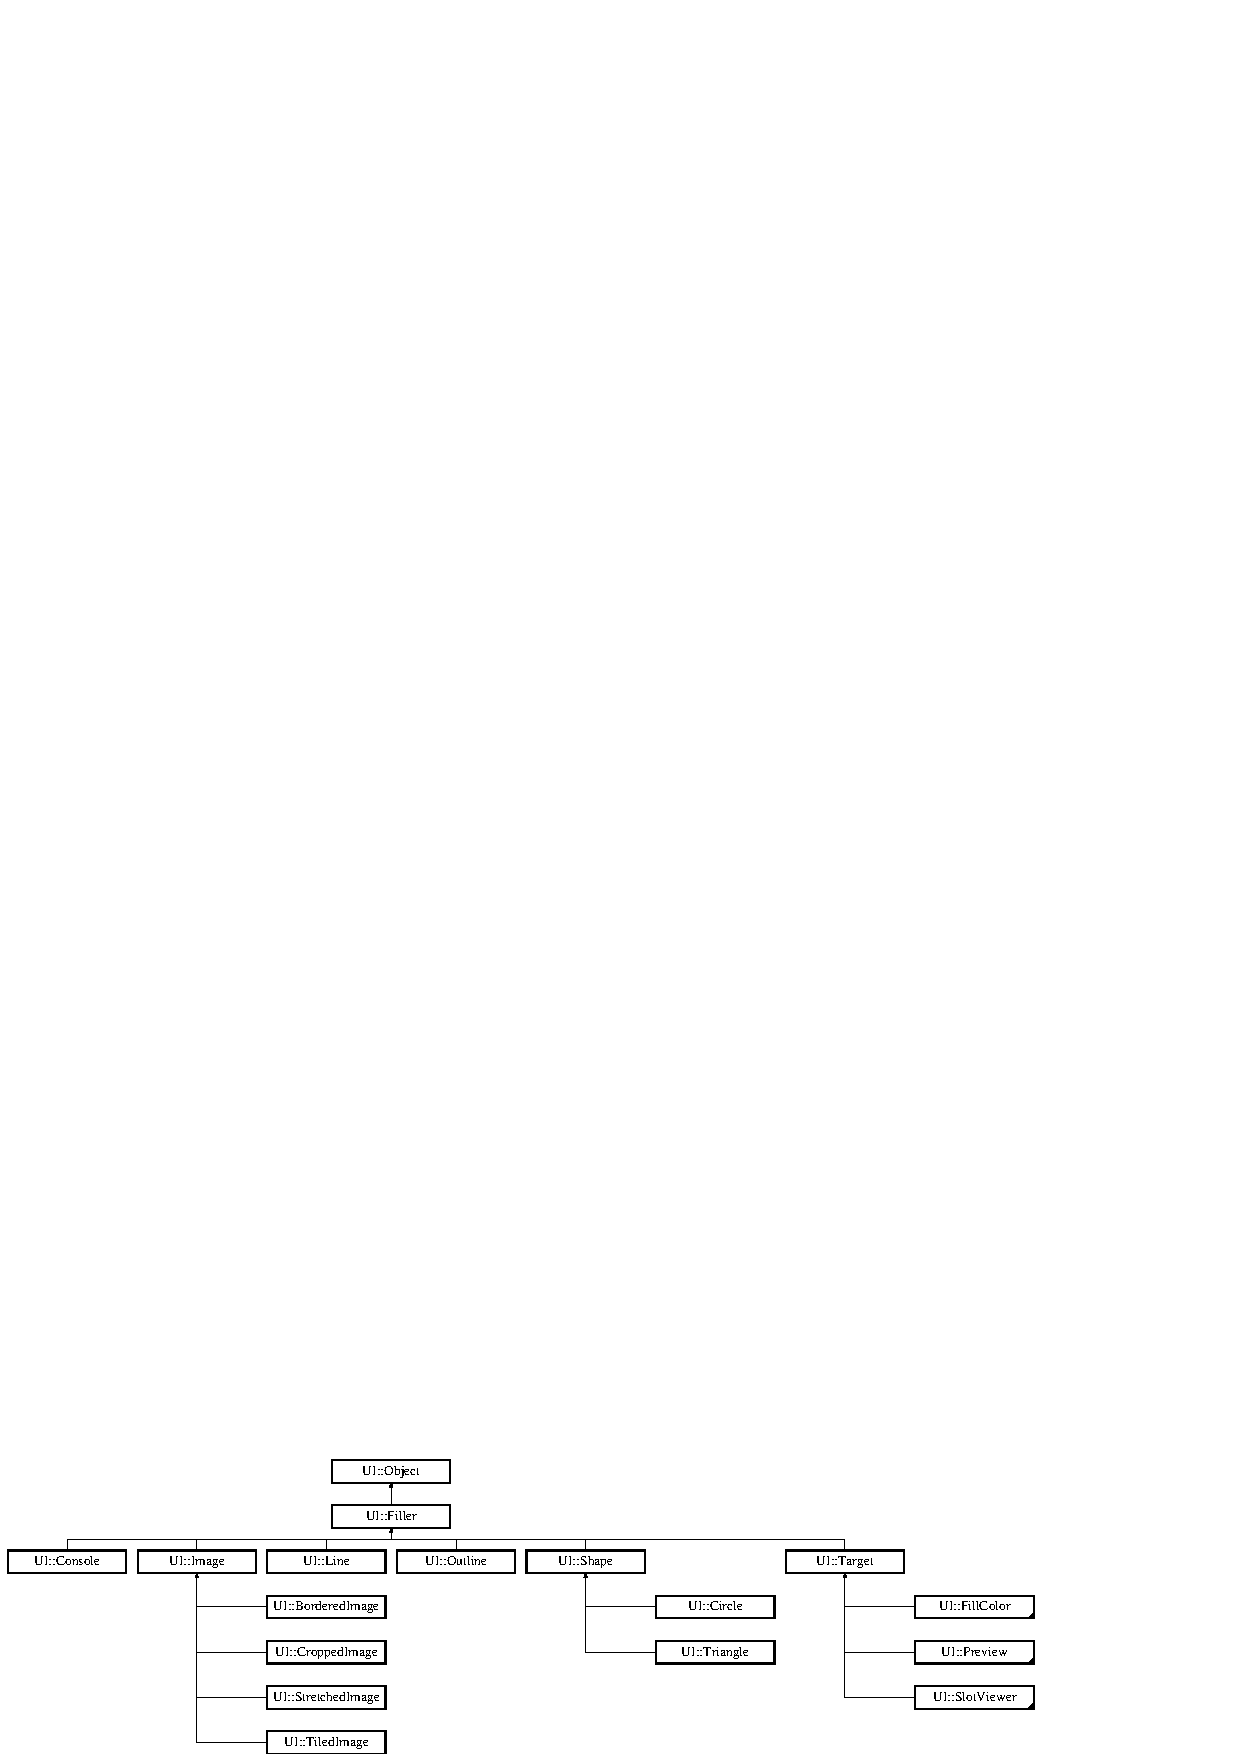
\includegraphics[height=3.951613cm]{struct_u_i_1_1_filler}
\end{center}
\end{figure}
\subsection*{Public Member Functions}
\begin{DoxyCompactItemize}
\item 
\mbox{\Hypertarget{struct_u_i_1_1_filler_a10fe0c7cb16fca977e060ac05fa2b0a9}\label{struct_u_i_1_1_filler_a10fe0c7cb16fca977e060ac05fa2b0a9}} 
void {\bfseries setup} (float minw\+\_\+, float minh\+\_\+)
\item 
\mbox{\Hypertarget{struct_u_i_1_1_filler_ac1e0b66287630c428e64a83fb04a19b4}\label{struct_u_i_1_1_filler_ac1e0b66287630c428e64a83fb04a19b4}} 
const char $\ast$ {\bfseries gettype} () const
\item 
\mbox{\Hypertarget{struct_u_i_1_1_filler_a6c7e90fe8c7aa157cbc2a5fe02dc1f1c}\label{struct_u_i_1_1_filler_a6c7e90fe8c7aa157cbc2a5fe02dc1f1c}} 
void {\bfseries layout} ()
\end{DoxyCompactItemize}
\subsection*{Static Public Member Functions}
\begin{DoxyCompactItemize}
\item 
\mbox{\Hypertarget{struct_u_i_1_1_filler_ac50b83a251dfb07f284bc599337b6963}\label{struct_u_i_1_1_filler_ac50b83a251dfb07f284bc599337b6963}} 
static const char $\ast$ {\bfseries typestr} ()
\end{DoxyCompactItemize}
\subsection*{Public Attributes}
\begin{DoxyCompactItemize}
\item 
\mbox{\Hypertarget{struct_u_i_1_1_filler_a9957d8052c2ca6d47c26376952a69ffc}\label{struct_u_i_1_1_filler_a9957d8052c2ca6d47c26376952a69ffc}} 
float {\bfseries minw}
\item 
\mbox{\Hypertarget{struct_u_i_1_1_filler_a5897a5bf89ce26db9d2c75688a34f1da}\label{struct_u_i_1_1_filler_a5897a5bf89ce26db9d2c75688a34f1da}} 
float {\bfseries minh}
\end{DoxyCompactItemize}


The documentation for this struct was generated from the following file\+:\begin{DoxyCompactItemize}
\item 
H\+:/\+Rival\+Engine/\+Rival\+\_\+\+Game\+\_\+\+Engine\+\_\+\+G\+I\+T/\+Rival3dengine/source/engine/ui.\+cpp\end{DoxyCompactItemize}

\hypertarget{structfireballrenderer}{}\section{fireballrenderer Struct Reference}
\label{structfireballrenderer}\index{fireballrenderer@{fireballrenderer}}
Inheritance diagram for fireballrenderer\+:\begin{figure}[H]
\begin{center}
\leavevmode
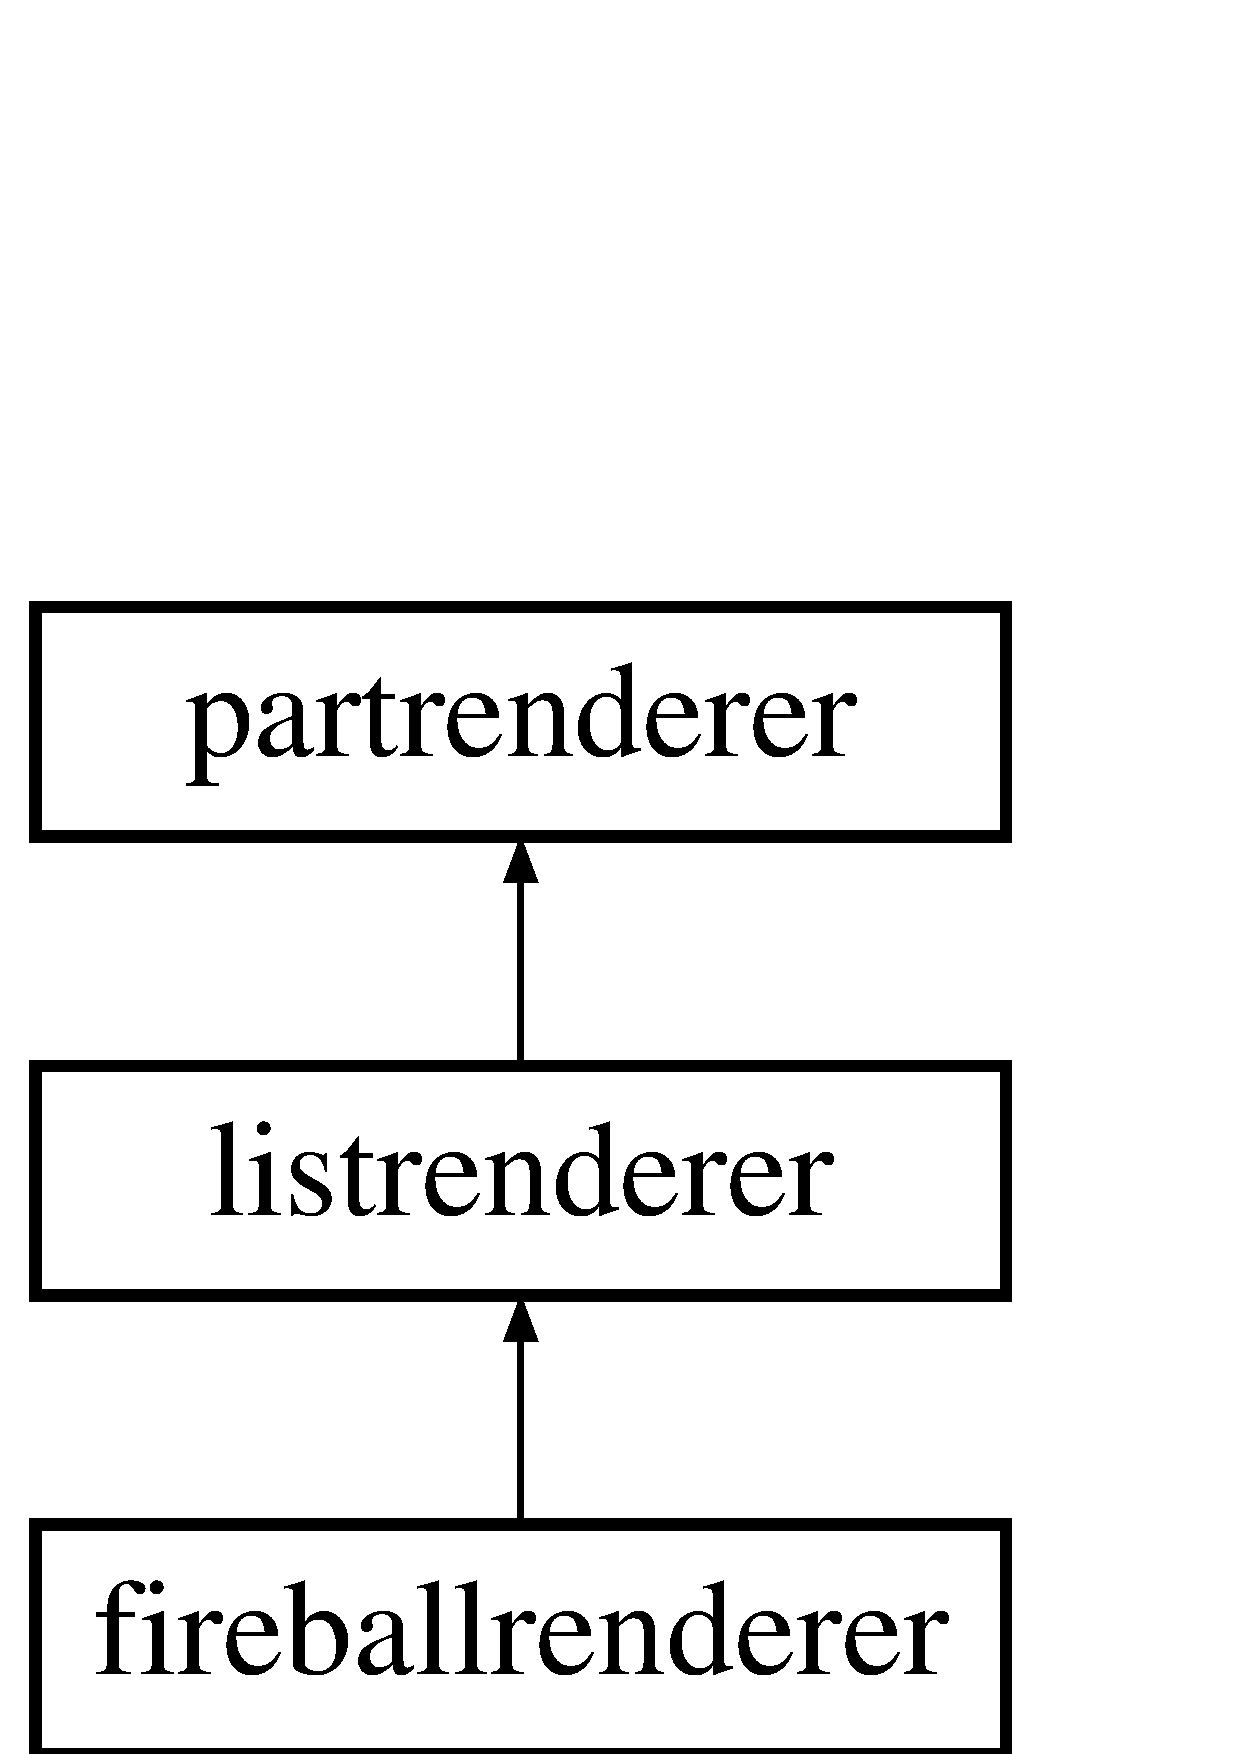
\includegraphics[height=3.000000cm]{structfireballrenderer}
\end{center}
\end{figure}
\subsection*{Public Member Functions}
\begin{DoxyCompactItemize}
\item 
\mbox{\Hypertarget{structfireballrenderer_ab3992508fffa9c1c6b9cedb9176af80d}\label{structfireballrenderer_ab3992508fffa9c1c6b9cedb9176af80d}} 
{\bfseries fireballrenderer} (const char $\ast$texname)
\item 
\mbox{\Hypertarget{structfireballrenderer_a0b40a6ece84870bca876d9167e61bcde}\label{structfireballrenderer_a0b40a6ece84870bca876d9167e61bcde}} 
void {\bfseries startrender} ()
\item 
\mbox{\Hypertarget{structfireballrenderer_a33dc996cf788481609db34931befce84}\label{structfireballrenderer_a33dc996cf788481609db34931befce84}} 
void {\bfseries endrender} ()
\item 
\mbox{\Hypertarget{structfireballrenderer_a3bc220d8feec217c8d40c3897011a072}\label{structfireballrenderer_a3bc220d8feec217c8d40c3897011a072}} 
void {\bfseries cleanup} ()
\item 
\mbox{\Hypertarget{structfireballrenderer_a83cccdc466e176976c2ebc6dda08c563}\label{structfireballrenderer_a83cccdc466e176976c2ebc6dda08c563}} 
void {\bfseries seedemitter} (\hyperlink{structparticleemitter}{particleemitter} \&pe, const \hyperlink{structvec}{vec} \&o, const \hyperlink{structvec}{vec} \&d, int fade, float size, int gravity)
\item 
\mbox{\Hypertarget{structfireballrenderer_ad5556d06bf0d507693da3971a1a9f74f}\label{structfireballrenderer_ad5556d06bf0d507693da3971a1a9f74f}} 
void {\bfseries renderpart} (\hyperlink{structlistparticle}{listparticle} $\ast$p, const \hyperlink{structvec}{vec} \&o, const \hyperlink{structvec}{vec} \&d, int blend, int ts)
\end{DoxyCompactItemize}
\subsection*{Additional Inherited Members}


The documentation for this struct was generated from the following file\+:\begin{DoxyCompactItemize}
\item 
H\+:/\+Rival\+Engine/\+Rival\+\_\+\+Game\+\_\+\+Engine\+\_\+\+G\+I\+T/\+Rival3dengine/source/engine/explosion.\+h\end{DoxyCompactItemize}

\hypertarget{structgame_1_1ctfclientmode_1_1flag}{}\section{game\+:\+:ctfclientmode\+:\+:flag Struct Reference}
\label{structgame_1_1ctfclientmode_1_1flag}\index{game\+::ctfclientmode\+::flag@{game\+::ctfclientmode\+::flag}}
\subsection*{Public Member Functions}
\begin{DoxyCompactItemize}
\item 
\mbox{\Hypertarget{structgame_1_1ctfclientmode_1_1flag_a1be2fea520554880c60cd4f115e6160d}\label{structgame_1_1ctfclientmode_1_1flag_a1be2fea520554880c60cd4f115e6160d}} 
void {\bfseries reset} ()
\item 
\mbox{\Hypertarget{structgame_1_1ctfclientmode_1_1flag_a75dc33c6193d592e45ca86085f8655e3}\label{structgame_1_1ctfclientmode_1_1flag_a75dc33c6193d592e45ca86085f8655e3}} 
\hyperlink{structvec}{vec} {\bfseries pos} () const
\end{DoxyCompactItemize}
\subsection*{Public Attributes}
\begin{DoxyCompactItemize}
\item 
\mbox{\Hypertarget{structgame_1_1ctfclientmode_1_1flag_adaed22bfa88507e94b8b81162299bfdd}\label{structgame_1_1ctfclientmode_1_1flag_adaed22bfa88507e94b8b81162299bfdd}} 
int {\bfseries id}
\item 
\mbox{\Hypertarget{structgame_1_1ctfclientmode_1_1flag_afa3ae8c65760f3683d0157972b22001a}\label{structgame_1_1ctfclientmode_1_1flag_afa3ae8c65760f3683d0157972b22001a}} 
int {\bfseries version}
\item 
\mbox{\Hypertarget{structgame_1_1ctfclientmode_1_1flag_a435e6a11c936d626e3109e49588fb321}\label{structgame_1_1ctfclientmode_1_1flag_a435e6a11c936d626e3109e49588fb321}} 
\hyperlink{structvec}{vec} {\bfseries droploc}
\item 
\mbox{\Hypertarget{structgame_1_1ctfclientmode_1_1flag_a8abefdae7e3ce8718386204e869316c1}\label{structgame_1_1ctfclientmode_1_1flag_a8abefdae7e3ce8718386204e869316c1}} 
\hyperlink{structvec}{vec} {\bfseries spawnloc}
\item 
\mbox{\Hypertarget{structgame_1_1ctfclientmode_1_1flag_a5a9f2fceeceedb6e6ee0678dddbf9587}\label{structgame_1_1ctfclientmode_1_1flag_a5a9f2fceeceedb6e6ee0678dddbf9587}} 
int {\bfseries team}
\item 
\mbox{\Hypertarget{structgame_1_1ctfclientmode_1_1flag_a87a856ca0b8ee3a3ab182e20d31b96d6}\label{structgame_1_1ctfclientmode_1_1flag_a87a856ca0b8ee3a3ab182e20d31b96d6}} 
int {\bfseries droptime}
\item 
\mbox{\Hypertarget{structgame_1_1ctfclientmode_1_1flag_ae48e48ef1e2f04d6dbeab6ed83591675}\label{structgame_1_1ctfclientmode_1_1flag_ae48e48ef1e2f04d6dbeab6ed83591675}} 
int {\bfseries owntime}
\item 
\mbox{\Hypertarget{structgame_1_1ctfclientmode_1_1flag_a1856cf80dd72afdadeebb38c5e128ab0}\label{structgame_1_1ctfclientmode_1_1flag_a1856cf80dd72afdadeebb38c5e128ab0}} 
\hyperlink{structgameent}{gameent} $\ast$ {\bfseries owner}
\item 
\mbox{\Hypertarget{structgame_1_1ctfclientmode_1_1flag_a52b71506c91ee8be744a437d0e8fccab}\label{structgame_1_1ctfclientmode_1_1flag_a52b71506c91ee8be744a437d0e8fccab}} 
float {\bfseries dropangle}
\item 
\mbox{\Hypertarget{structgame_1_1ctfclientmode_1_1flag_a3b9630ed348170ab8ce4a8cf9ad11874}\label{structgame_1_1ctfclientmode_1_1flag_a3b9630ed348170ab8ce4a8cf9ad11874}} 
float {\bfseries spawnangle}
\item 
\mbox{\Hypertarget{structgame_1_1ctfclientmode_1_1flag_a6df7e9032c50c3157e36d0f7a3939036}\label{structgame_1_1ctfclientmode_1_1flag_a6df7e9032c50c3157e36d0f7a3939036}} 
\hyperlink{structvec}{vec} {\bfseries interploc}
\item 
\mbox{\Hypertarget{structgame_1_1ctfclientmode_1_1flag_af4752fae0780589f155f1af89de3692f}\label{structgame_1_1ctfclientmode_1_1flag_af4752fae0780589f155f1af89de3692f}} 
float {\bfseries interpangle}
\item 
\mbox{\Hypertarget{structgame_1_1ctfclientmode_1_1flag_ad16c49fc668cb293c3a15872c20aa736}\label{structgame_1_1ctfclientmode_1_1flag_ad16c49fc668cb293c3a15872c20aa736}} 
int {\bfseries interptime}
\end{DoxyCompactItemize}


The documentation for this struct was generated from the following file\+:\begin{DoxyCompactItemize}
\item 
H\+:/\+Rival\+Engine/\+Rival\+\_\+\+Game\+\_\+\+Engine\+\_\+\+G\+I\+T/\+Rival3dengine/source/game/client.\+cpp\end{DoxyCompactItemize}

\hypertarget{structctfclientmode_1_1flag}{}\section{ctfclientmode\+:\+:flag Struct Reference}
\label{structctfclientmode_1_1flag}\index{ctfclientmode\+::flag@{ctfclientmode\+::flag}}
\subsection*{Public Member Functions}
\begin{DoxyCompactItemize}
\item 
\mbox{\Hypertarget{structctfclientmode_1_1flag_ad9d0a8d57659004a1d16ebb7945c3d8a}\label{structctfclientmode_1_1flag_ad9d0a8d57659004a1d16ebb7945c3d8a}} 
void {\bfseries reset} ()
\item 
\mbox{\Hypertarget{structctfclientmode_1_1flag_a03511d40e10b8c359f2ff20c4279eadc}\label{structctfclientmode_1_1flag_a03511d40e10b8c359f2ff20c4279eadc}} 
\hyperlink{structvec}{vec} {\bfseries pos} () const
\end{DoxyCompactItemize}
\subsection*{Public Attributes}
\begin{DoxyCompactItemize}
\item 
\mbox{\Hypertarget{structctfclientmode_1_1flag_a15b55bac4719a6fa34243b86064fb8f8}\label{structctfclientmode_1_1flag_a15b55bac4719a6fa34243b86064fb8f8}} 
int {\bfseries id}
\item 
\mbox{\Hypertarget{structctfclientmode_1_1flag_aa15e505761ffbc1a47bcf927931a71c0}\label{structctfclientmode_1_1flag_aa15e505761ffbc1a47bcf927931a71c0}} 
int {\bfseries version}
\item 
\mbox{\Hypertarget{structctfclientmode_1_1flag_abd568699f3000038108211f768c9393e}\label{structctfclientmode_1_1flag_abd568699f3000038108211f768c9393e}} 
\hyperlink{structvec}{vec} {\bfseries droploc}
\item 
\mbox{\Hypertarget{structctfclientmode_1_1flag_a15ff93e390342b98fb26cf92df6c6e8b}\label{structctfclientmode_1_1flag_a15ff93e390342b98fb26cf92df6c6e8b}} 
\hyperlink{structvec}{vec} {\bfseries spawnloc}
\item 
\mbox{\Hypertarget{structctfclientmode_1_1flag_ab2fe1a8898208d832f85be7fcc2242e1}\label{structctfclientmode_1_1flag_ab2fe1a8898208d832f85be7fcc2242e1}} 
int {\bfseries team}
\item 
\mbox{\Hypertarget{structctfclientmode_1_1flag_ac1a6380fdbedb915800aac2bc57bdec9}\label{structctfclientmode_1_1flag_ac1a6380fdbedb915800aac2bc57bdec9}} 
int {\bfseries droptime}
\item 
\mbox{\Hypertarget{structctfclientmode_1_1flag_af5076fc52d0c59642e93ad534c942de5}\label{structctfclientmode_1_1flag_af5076fc52d0c59642e93ad534c942de5}} 
int {\bfseries owntime}
\item 
\mbox{\Hypertarget{structctfclientmode_1_1flag_affcf09e57c1b604a32a0affa1635da7c}\label{structctfclientmode_1_1flag_affcf09e57c1b604a32a0affa1635da7c}} 
\hyperlink{structgameent}{gameent} $\ast$ {\bfseries owner}
\item 
\mbox{\Hypertarget{structctfclientmode_1_1flag_adae9b4753be8bb38df40a26b9fe3853d}\label{structctfclientmode_1_1flag_adae9b4753be8bb38df40a26b9fe3853d}} 
float {\bfseries dropangle}
\item 
\mbox{\Hypertarget{structctfclientmode_1_1flag_afc2b989066184fcaff4547d29f2c2b63}\label{structctfclientmode_1_1flag_afc2b989066184fcaff4547d29f2c2b63}} 
float {\bfseries spawnangle}
\item 
\mbox{\Hypertarget{structctfclientmode_1_1flag_ab7d642430fd3e17b033a36bf56d0b220}\label{structctfclientmode_1_1flag_ab7d642430fd3e17b033a36bf56d0b220}} 
\hyperlink{structvec}{vec} {\bfseries interploc}
\item 
\mbox{\Hypertarget{structctfclientmode_1_1flag_a54f3cd691c1113fc8f2ac4c794a6c158}\label{structctfclientmode_1_1flag_a54f3cd691c1113fc8f2ac4c794a6c158}} 
float {\bfseries interpangle}
\item 
\mbox{\Hypertarget{structctfclientmode_1_1flag_a0d3ac7ef75e6cc5319335b49186a23c3}\label{structctfclientmode_1_1flag_a0d3ac7ef75e6cc5319335b49186a23c3}} 
int {\bfseries interptime}
\end{DoxyCompactItemize}


The documentation for this struct was generated from the following file\+:\begin{DoxyCompactItemize}
\item 
H\+:/\+Rival\+Engine/\+Rival\+\_\+\+Game\+\_\+\+Engine\+\_\+\+G\+I\+T/\+Rival3dengine/source/game/ctf.\+h\end{DoxyCompactItemize}

\hypertarget{structserver_1_1ctfservmode_1_1flag}{}\section{server\+:\+:ctfservmode\+:\+:flag Struct Reference}
\label{structserver_1_1ctfservmode_1_1flag}\index{server\+::ctfservmode\+::flag@{server\+::ctfservmode\+::flag}}
\subsection*{Public Member Functions}
\begin{DoxyCompactItemize}
\item 
\mbox{\Hypertarget{structserver_1_1ctfservmode_1_1flag_a015a8047e69ef53858188c04de595d84}\label{structserver_1_1ctfservmode_1_1flag_a015a8047e69ef53858188c04de595d84}} 
void {\bfseries reset} ()
\end{DoxyCompactItemize}
\subsection*{Public Attributes}
\begin{DoxyCompactItemize}
\item 
\mbox{\Hypertarget{structserver_1_1ctfservmode_1_1flag_a9872994fb4cd07f744f9567905588af3}\label{structserver_1_1ctfservmode_1_1flag_a9872994fb4cd07f744f9567905588af3}} 
int {\bfseries id}
\item 
\mbox{\Hypertarget{structserver_1_1ctfservmode_1_1flag_a95ac67e3b80d4eb397687a1dd1fb6880}\label{structserver_1_1ctfservmode_1_1flag_a95ac67e3b80d4eb397687a1dd1fb6880}} 
int {\bfseries version}
\item 
\mbox{\Hypertarget{structserver_1_1ctfservmode_1_1flag_ab06265abf0f8da3f98b26e2c75731fb0}\label{structserver_1_1ctfservmode_1_1flag_ab06265abf0f8da3f98b26e2c75731fb0}} 
\hyperlink{structvec}{vec} {\bfseries droploc}
\item 
\mbox{\Hypertarget{structserver_1_1ctfservmode_1_1flag_a29a3024f10d4b82b5741372f501327e4}\label{structserver_1_1ctfservmode_1_1flag_a29a3024f10d4b82b5741372f501327e4}} 
\hyperlink{structvec}{vec} {\bfseries spawnloc}
\item 
\mbox{\Hypertarget{structserver_1_1ctfservmode_1_1flag_a81ff28e7eecdfa7864656839903fdcde}\label{structserver_1_1ctfservmode_1_1flag_a81ff28e7eecdfa7864656839903fdcde}} 
int {\bfseries team}
\item 
\mbox{\Hypertarget{structserver_1_1ctfservmode_1_1flag_a37ef955b71e5bb6d5993e640d9738f9a}\label{structserver_1_1ctfservmode_1_1flag_a37ef955b71e5bb6d5993e640d9738f9a}} 
int {\bfseries droptime}
\item 
\mbox{\Hypertarget{structserver_1_1ctfservmode_1_1flag_a981ba8ab7b0dd7f5da9de2320ebf4d43}\label{structserver_1_1ctfservmode_1_1flag_a981ba8ab7b0dd7f5da9de2320ebf4d43}} 
int {\bfseries owntime}
\item 
\mbox{\Hypertarget{structserver_1_1ctfservmode_1_1flag_a42ba45f1b657132547d019c69e2828d7}\label{structserver_1_1ctfservmode_1_1flag_a42ba45f1b657132547d019c69e2828d7}} 
int {\bfseries owner}
\item 
\mbox{\Hypertarget{structserver_1_1ctfservmode_1_1flag_a46d02fd0ea807adc371793fef2fc214a}\label{structserver_1_1ctfservmode_1_1flag_a46d02fd0ea807adc371793fef2fc214a}} 
int {\bfseries dropcount}
\item 
\mbox{\Hypertarget{structserver_1_1ctfservmode_1_1flag_af62ed239084261f14803c788ce81332b}\label{structserver_1_1ctfservmode_1_1flag_af62ed239084261f14803c788ce81332b}} 
int {\bfseries dropper}
\end{DoxyCompactItemize}


The documentation for this struct was generated from the following file\+:\begin{DoxyCompactItemize}
\item 
H\+:/\+Rival\+Engine/\+Rival\+\_\+\+Game\+\_\+\+Engine\+\_\+\+G\+I\+T/\+Rival3dengine/source/game/server.\+cpp\end{DoxyCompactItemize}

\hypertarget{structflare}{}\section{flare Struct Reference}
\label{structflare}\index{flare@{flare}}
\subsection*{Public Attributes}
\begin{DoxyCompactItemize}
\item 
\mbox{\Hypertarget{structflare_a89e957da6aca75ee9cfdf73a6ae136bd}\label{structflare_a89e957da6aca75ee9cfdf73a6ae136bd}} 
\hyperlink{structvec}{vec} {\bfseries o}
\item 
\mbox{\Hypertarget{structflare_a0c9e10d342303a31b7a8739cc989af33}\label{structflare_a0c9e10d342303a31b7a8739cc989af33}} 
\hyperlink{structvec}{vec} {\bfseries center}
\item 
\mbox{\Hypertarget{structflare_adb73b49f163d75603ef91e90b0b9a122}\label{structflare_adb73b49f163d75603ef91e90b0b9a122}} 
float {\bfseries size}
\item 
\mbox{\Hypertarget{structflare_a47a882e32bed95aa29077e5c406eedcf}\label{structflare_a47a882e32bed95aa29077e5c406eedcf}} 
\hyperlink{structbvec}{bvec} {\bfseries color}
\item 
\mbox{\Hypertarget{structflare_af98f143a318885ea5f64fcd6f99a282f}\label{structflare_af98f143a318885ea5f64fcd6f99a282f}} 
bool {\bfseries sparkle}
\end{DoxyCompactItemize}


The documentation for this struct was generated from the following file\+:\begin{DoxyCompactItemize}
\item 
H\+:/\+Rival\+Engine/\+Rival\+\_\+\+Game\+\_\+\+Engine\+\_\+\+G\+I\+T/\+Rival3dengine/source/engine/lensflare.\+h\end{DoxyCompactItemize}

\hypertarget{structflarerenderer}{}\section{flarerenderer Struct Reference}
\label{structflarerenderer}\index{flarerenderer@{flarerenderer}}
Inheritance diagram for flarerenderer\+:\begin{figure}[H]
\begin{center}
\leavevmode
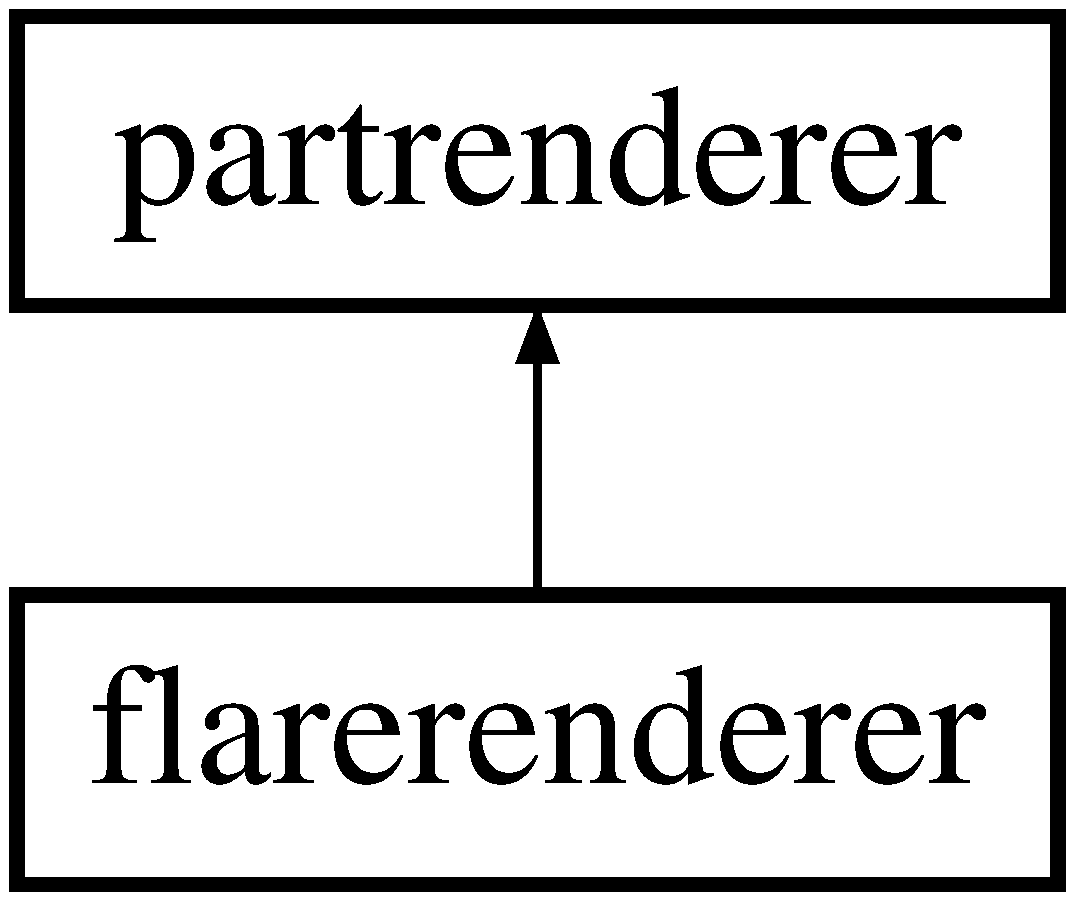
\includegraphics[height=2.000000cm]{structflarerenderer}
\end{center}
\end{figure}
\subsection*{Public Member Functions}
\begin{DoxyCompactItemize}
\item 
\mbox{\Hypertarget{structflarerenderer_ac97df023d8f71a1c1ec054f553717327}\label{structflarerenderer_ac97df023d8f71a1c1ec054f553717327}} 
{\bfseries flarerenderer} (const char $\ast$texname, int maxflares, int flags=0)
\item 
\mbox{\Hypertarget{structflarerenderer_a507f569a42c4691c36d18a11be02f568}\label{structflarerenderer_a507f569a42c4691c36d18a11be02f568}} 
void {\bfseries reset} ()
\item 
\mbox{\Hypertarget{structflarerenderer_a619a5cbea2fc100eea3e6719faf20560}\label{structflarerenderer_a619a5cbea2fc100eea3e6719faf20560}} 
void {\bfseries newflare} (\hyperlink{structvec}{vec} \&o, const \hyperlink{structvec}{vec} \&center, uchar r, uchar g, uchar b, float mod, float size, bool sun, bool sparkle)
\item 
\mbox{\Hypertarget{structflarerenderer_a5728a8911a1b72baff700f7ed62bc170}\label{structflarerenderer_a5728a8911a1b72baff700f7ed62bc170}} 
void {\bfseries addflare} (\hyperlink{structvec}{vec} \&o, uchar r, uchar g, uchar b, bool sun, bool sparkle)
\item 
\mbox{\Hypertarget{structflarerenderer_ace67d99d288d22df7474fc6bf29e4a0c}\label{structflarerenderer_ace67d99d288d22df7474fc6bf29e4a0c}} 
void {\bfseries update} ()
\item 
\mbox{\Hypertarget{structflarerenderer_a873860d2dfe149a5dd25507adc8d0be3}\label{structflarerenderer_a873860d2dfe149a5dd25507adc8d0be3}} 
int {\bfseries count} ()
\item 
\mbox{\Hypertarget{structflarerenderer_af4c0e43f0d812d08fe5ace60253d5fff}\label{structflarerenderer_af4c0e43f0d812d08fe5ace60253d5fff}} 
bool {\bfseries haswork} ()
\item 
\mbox{\Hypertarget{structflarerenderer_adaca66769e01a785c13665807578f746}\label{structflarerenderer_adaca66769e01a785c13665807578f746}} 
void {\bfseries render} ()
\item 
\mbox{\Hypertarget{structflarerenderer_a056b5bf69a27848ce80f40e0d0288b76}\label{structflarerenderer_a056b5bf69a27848ce80f40e0d0288b76}} 
\hyperlink{structparticle}{particle} $\ast$ {\bfseries addpart} (const \hyperlink{structvec}{vec} \&o, const \hyperlink{structvec}{vec} \&d, int fade, int color, float size, int gravity=0)
\end{DoxyCompactItemize}
\subsection*{Public Attributes}
\begin{DoxyCompactItemize}
\item 
\mbox{\Hypertarget{structflarerenderer_a6cc2764f704fa0e83256434bd12de3d1}\label{structflarerenderer_a6cc2764f704fa0e83256434bd12de3d1}} 
int {\bfseries maxflares}
\item 
\mbox{\Hypertarget{structflarerenderer_aa3d46257da2cc518f173e95af9c14970}\label{structflarerenderer_aa3d46257da2cc518f173e95af9c14970}} 
int {\bfseries numflares}
\item 
\mbox{\Hypertarget{structflarerenderer_ada2be781832a25529330a75c151f42f3}\label{structflarerenderer_ada2be781832a25529330a75c151f42f3}} 
unsigned int {\bfseries shinetime}
\item 
\mbox{\Hypertarget{structflarerenderer_af19c40c54dfc00415be611c8419d61e4}\label{structflarerenderer_af19c40c54dfc00415be611c8419d61e4}} 
\hyperlink{structflare}{flare} $\ast$ {\bfseries flares}
\end{DoxyCompactItemize}


The documentation for this struct was generated from the following file\+:\begin{DoxyCompactItemize}
\item 
H\+:/\+Rival\+Engine/\+Rival\+\_\+\+Game\+\_\+\+Engine\+\_\+\+G\+I\+T/\+Rival3dengine/source/engine/lensflare.\+h\end{DoxyCompactItemize}

\hypertarget{structfont}{}\section{font Struct Reference}
\label{structfont}\index{font@{font}}
\subsection*{Classes}
\begin{DoxyCompactItemize}
\item 
struct \hyperlink{structfont_1_1charinfo}{charinfo}
\end{DoxyCompactItemize}
\subsection*{Public Attributes}
\begin{DoxyCompactItemize}
\item 
\mbox{\Hypertarget{structfont_a4f4ca5bd44caf8697240668945a78ded}\label{structfont_a4f4ca5bd44caf8697240668945a78ded}} 
char $\ast$ {\bfseries name}
\item 
\mbox{\Hypertarget{structfont_a478d56e65e8c23e3d5d91cc7abbc6702}\label{structfont_a478d56e65e8c23e3d5d91cc7abbc6702}} 
\hyperlink{structvector}{vector}$<$ \hyperlink{struct_texture}{Texture} $\ast$ $>$ {\bfseries texs}
\item 
\mbox{\Hypertarget{structfont_a31521ec273db00b71b69ea06fbce4d2b}\label{structfont_a31521ec273db00b71b69ea06fbce4d2b}} 
\hyperlink{structvector}{vector}$<$ \hyperlink{structfont_1_1charinfo}{charinfo} $>$ {\bfseries chars}
\item 
\mbox{\Hypertarget{structfont_a89d8a2a1bc40395d3405b4acf4dff53c}\label{structfont_a89d8a2a1bc40395d3405b4acf4dff53c}} 
int {\bfseries charoffset}
\item 
\mbox{\Hypertarget{structfont_ab29587e54e84bd0e74a87829432efe10}\label{structfont_ab29587e54e84bd0e74a87829432efe10}} 
int {\bfseries defaultw}
\item 
\mbox{\Hypertarget{structfont_ae9374c8aaacc1a18d77cc79293238ae3}\label{structfont_ae9374c8aaacc1a18d77cc79293238ae3}} 
int {\bfseries defaulth}
\item 
\mbox{\Hypertarget{structfont_a100f003b0a274f161d59d4040d238d09}\label{structfont_a100f003b0a274f161d59d4040d238d09}} 
int {\bfseries scale}
\item 
\mbox{\Hypertarget{structfont_adc29dda614b782a1a1855070eaf62446}\label{structfont_adc29dda614b782a1a1855070eaf62446}} 
float {\bfseries bordermin}
\item 
\mbox{\Hypertarget{structfont_a786747e3d9be1bb770b21c98659b858d}\label{structfont_a786747e3d9be1bb770b21c98659b858d}} 
float {\bfseries bordermax}
\item 
\mbox{\Hypertarget{structfont_a90976c1d63176f8a306d03bbe9e98d1e}\label{structfont_a90976c1d63176f8a306d03bbe9e98d1e}} 
float {\bfseries outlinemin}
\item 
\mbox{\Hypertarget{structfont_a1a5f6a3f1360b65603ef0d69614dde47}\label{structfont_a1a5f6a3f1360b65603ef0d69614dde47}} 
float {\bfseries outlinemax}
\end{DoxyCompactItemize}


The documentation for this struct was generated from the following file\+:\begin{DoxyCompactItemize}
\item 
H\+:/\+Rival\+Engine/\+Rival\+\_\+\+Game\+\_\+\+Engine\+\_\+\+G\+I\+T/\+Rival3dengine/source/engine/engine.\+h\end{DoxyCompactItemize}

\hypertarget{struct_u_i_1_1_font}{}\section{UI\+:\+:Font Struct Reference}
\label{struct_u_i_1_1_font}\index{U\+I\+::\+Font@{U\+I\+::\+Font}}
Inheritance diagram for UI\+:\+:Font\+:\begin{figure}[H]
\begin{center}
\leavevmode
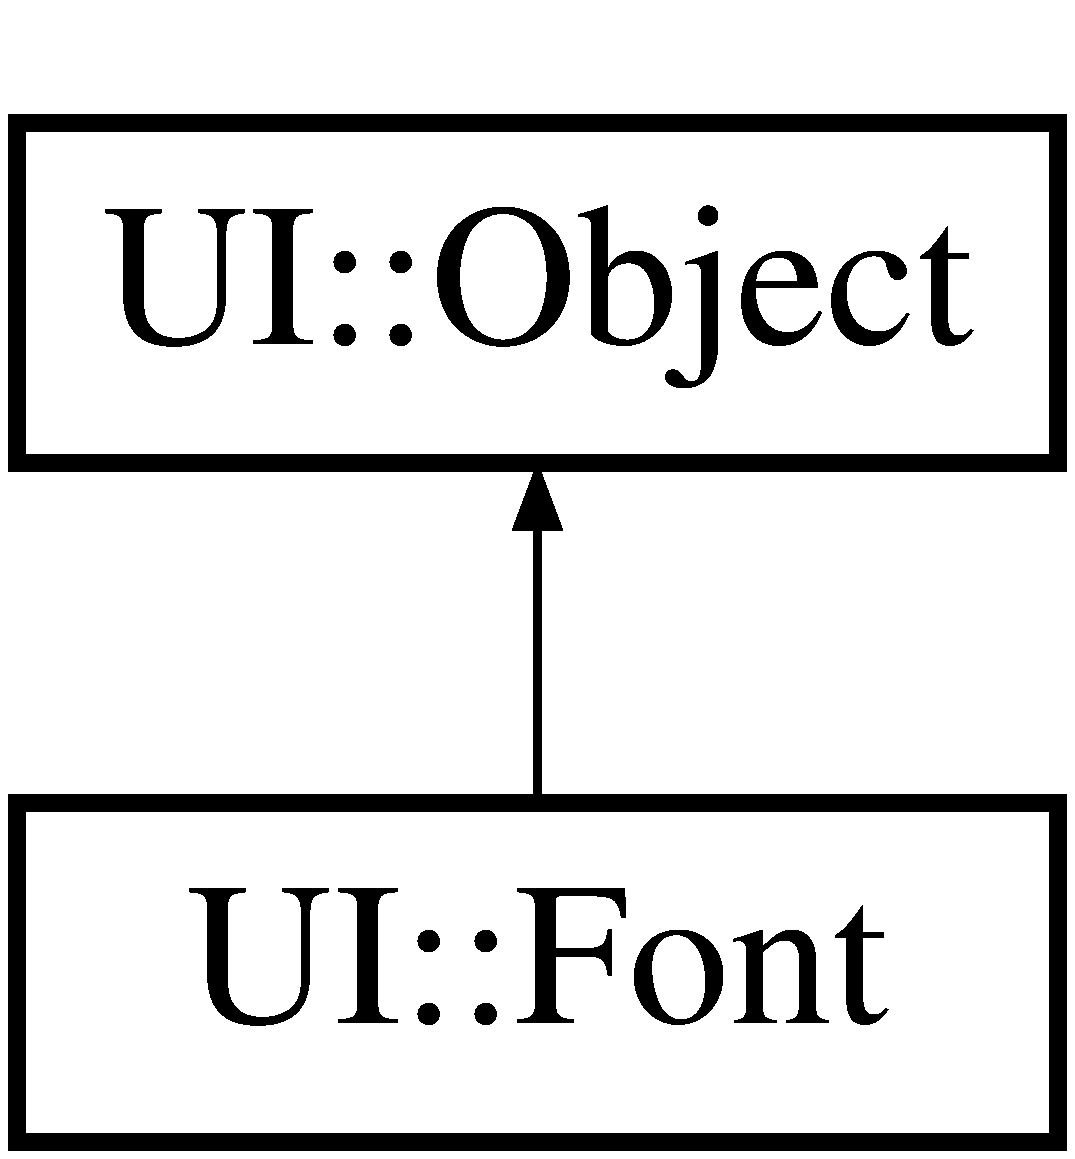
\includegraphics[height=2.000000cm]{struct_u_i_1_1_font}
\end{center}
\end{figure}
\subsection*{Public Member Functions}
\begin{DoxyCompactItemize}
\item 
\mbox{\Hypertarget{struct_u_i_1_1_font_ad6b9e2f97ac4312331ee845f49f1ba53}\label{struct_u_i_1_1_font_ad6b9e2f97ac4312331ee845f49f1ba53}} 
void {\bfseries setup} (const char $\ast$name)
\item 
\mbox{\Hypertarget{struct_u_i_1_1_font_ad838ccf603bf00782d78f1705041c494}\label{struct_u_i_1_1_font_ad838ccf603bf00782d78f1705041c494}} 
void {\bfseries layout} ()
\item 
\mbox{\Hypertarget{struct_u_i_1_1_font_abce1c14d18d6273df557586e87ca01c4}\label{struct_u_i_1_1_font_abce1c14d18d6273df557586e87ca01c4}} 
void {\bfseries draw} (float sx, float sy)
\item 
\mbox{\Hypertarget{struct_u_i_1_1_font_a6dbdd42df4dd7178e7655401db026454}\label{struct_u_i_1_1_font_a6dbdd42df4dd7178e7655401db026454}} 
void {\bfseries buildchildren} (uint $\ast$contents)
\item 
\mbox{\Hypertarget{struct_u_i_1_1_font_a4922bd8494ec4a005d9accc3e7f8ccbb}\label{struct_u_i_1_1_font_a4922bd8494ec4a005d9accc3e7f8ccbb}} 
D\+O\+S\+T\+A\+T\+ES bool {\bfseries rawkey} (int code, bool isdown)
\item 
\mbox{\Hypertarget{struct_u_i_1_1_font_a8187702e45f52717d6fc339280593e97}\label{struct_u_i_1_1_font_a8187702e45f52717d6fc339280593e97}} 
bool {\bfseries key} (int code, bool isdown)
\item 
\mbox{\Hypertarget{struct_u_i_1_1_font_ac4803a16fdd7a3d34b39fde36d7122af}\label{struct_u_i_1_1_font_ac4803a16fdd7a3d34b39fde36d7122af}} 
bool {\bfseries textinput} (const char $\ast$str, int len)
\end{DoxyCompactItemize}
\subsection*{Public Attributes}
\begin{DoxyCompactItemize}
\item 
\mbox{\Hypertarget{struct_u_i_1_1_font_ac9674071551e52887851a6a60f0e8757}\label{struct_u_i_1_1_font_ac9674071551e52887851a6a60f0e8757}} 
\+::\hyperlink{structfont}{font} $\ast$ {\bfseries font}
\end{DoxyCompactItemize}
\subsection*{Additional Inherited Members}


The documentation for this struct was generated from the following file\+:\begin{DoxyCompactItemize}
\item 
H\+:/\+Rival\+Engine/\+Rival\+\_\+\+Game\+\_\+\+Engine\+\_\+\+G\+I\+T/\+Rival3dengine/source/engine/ui.\+cpp\end{DoxyCompactItemize}

\hypertarget{structfontchar}{}\section{fontchar Struct Reference}
\label{structfontchar}\index{fontchar@{fontchar}}
\subsection*{Public Attributes}
\begin{DoxyCompactItemize}
\item 
\mbox{\Hypertarget{structfontchar_a5b75429ff655bda1fae43bba91c30109}\label{structfontchar_a5b75429ff655bda1fae43bba91c30109}} 
int {\bfseries code}
\item 
\mbox{\Hypertarget{structfontchar_a2c5a26a10fed40d19840cc2be99cb466}\label{structfontchar_a2c5a26a10fed40d19840cc2be99cb466}} 
int {\bfseries uni}
\item 
\mbox{\Hypertarget{structfontchar_a61ac569a542afe35acaa01c76b6ed7e6}\label{structfontchar_a61ac569a542afe35acaa01c76b6ed7e6}} 
int {\bfseries tex}
\item 
\mbox{\Hypertarget{structfontchar_a0a8dcacee2bf0a1b8467f97c65e8b661}\label{structfontchar_a0a8dcacee2bf0a1b8467f97c65e8b661}} 
int {\bfseries x}
\item 
\mbox{\Hypertarget{structfontchar_a00b75e11ac16114f3c39985b85f1a532}\label{structfontchar_a00b75e11ac16114f3c39985b85f1a532}} 
int {\bfseries y}
\item 
\mbox{\Hypertarget{structfontchar_ac7943e75638557bde99d7ad099b70b1a}\label{structfontchar_ac7943e75638557bde99d7ad099b70b1a}} 
int {\bfseries sdfradius}
\item 
\mbox{\Hypertarget{structfontchar_aa05297ae69315d59535360f5715b417c}\label{structfontchar_aa05297ae69315d59535360f5715b417c}} 
int {\bfseries sdfpitch}
\item 
\mbox{\Hypertarget{structfontchar_a02a7208625d7d22d423a2a7e014ea89d}\label{structfontchar_a02a7208625d7d22d423a2a7e014ea89d}} 
int {\bfseries sdfx}
\item 
\mbox{\Hypertarget{structfontchar_a7543ff67135154fcafc2d7e54984791e}\label{structfontchar_a7543ff67135154fcafc2d7e54984791e}} 
int {\bfseries sdfy}
\item 
\mbox{\Hypertarget{structfontchar_a2c7b533d098a3eb6955ee3d77235636d}\label{structfontchar_a2c7b533d098a3eb6955ee3d77235636d}} 
int {\bfseries sdfw}
\item 
\mbox{\Hypertarget{structfontchar_aef2bbf1a28f329614a640fb013e2be68}\label{structfontchar_aef2bbf1a28f329614a640fb013e2be68}} 
int {\bfseries sdfh}
\item 
\mbox{\Hypertarget{structfontchar_a086485155f05cb86a2e44d60dbf4634c}\label{structfontchar_a086485155f05cb86a2e44d60dbf4634c}} 
float {\bfseries w}
\item 
\mbox{\Hypertarget{structfontchar_a159d9cbcba1fe394ac736f3a9f6971f9}\label{structfontchar_a159d9cbcba1fe394ac736f3a9f6971f9}} 
float {\bfseries h}
\item 
\mbox{\Hypertarget{structfontchar_aff0af280b7203e045ba5910e60b2b27c}\label{structfontchar_aff0af280b7203e045ba5910e60b2b27c}} 
float {\bfseries left}
\item 
\mbox{\Hypertarget{structfontchar_ae7d031a9ba0b4b84b9b216ecbac3b456}\label{structfontchar_ae7d031a9ba0b4b84b9b216ecbac3b456}} 
float {\bfseries top}
\item 
\mbox{\Hypertarget{structfontchar_a39f4f3e3675bbe4a59d242d7daa03057}\label{structfontchar_a39f4f3e3675bbe4a59d242d7daa03057}} 
float {\bfseries advance}
\item 
\mbox{\Hypertarget{structfontchar_af4a234a7ee03abb3f3696739d31d9f8c}\label{structfontchar_af4a234a7ee03abb3f3696739d31d9f8c}} 
F\+T\+\_\+\+Bitmap\+Glyph {\bfseries glyph}
\item 
\mbox{\Hypertarget{structfontchar_ae2fad7dd8115c16822a9efba4fe13809}\label{structfontchar_ae2fad7dd8115c16822a9efba4fe13809}} 
uchar $\ast$ {\bfseries sdf}
\end{DoxyCompactItemize}


The documentation for this struct was generated from the following file\+:\begin{DoxyCompactItemize}
\item 
H\+:/\+Rival\+Engine/\+Rival\+\_\+\+Game\+\_\+\+Engine\+\_\+\+G\+I\+T/\+Rival3dengine/source/shared/tessfont.\+c\end{DoxyCompactItemize}

\hypertarget{struct_frag_data_loc}{}\section{Frag\+Data\+Loc Struct Reference}
\label{struct_frag_data_loc}\index{Frag\+Data\+Loc@{Frag\+Data\+Loc}}
\subsection*{Public Member Functions}
\begin{DoxyCompactItemize}
\item 
\mbox{\Hypertarget{struct_frag_data_loc_a2c5c1b4eb2518ef2cac825f15562d0f3}\label{struct_frag_data_loc_a2c5c1b4eb2518ef2cac825f15562d0f3}} 
{\bfseries Frag\+Data\+Loc} (const char $\ast$name=N\+U\+LL, int loc=-\/1, G\+Lenum format=G\+L\+\_\+\+F\+A\+L\+SE, int index=0)
\end{DoxyCompactItemize}
\subsection*{Public Attributes}
\begin{DoxyCompactItemize}
\item 
\mbox{\Hypertarget{struct_frag_data_loc_a55fa44cb54807d0d85b3833f63bced0a}\label{struct_frag_data_loc_a55fa44cb54807d0d85b3833f63bced0a}} 
const char $\ast$ {\bfseries name}
\item 
\mbox{\Hypertarget{struct_frag_data_loc_a4df9db5ce8f0976850f6937ca06555ca}\label{struct_frag_data_loc_a4df9db5ce8f0976850f6937ca06555ca}} 
int {\bfseries loc}
\item 
\mbox{\Hypertarget{struct_frag_data_loc_afa4ff3fd93ca271c1b2405fad3b54cf6}\label{struct_frag_data_loc_afa4ff3fd93ca271c1b2405fad3b54cf6}} 
G\+Lenum {\bfseries format}
\item 
\mbox{\Hypertarget{struct_frag_data_loc_a0ca3bc3d6df2cb757182040e8dcab5fe}\label{struct_frag_data_loc_a0ca3bc3d6df2cb757182040e8dcab5fe}} 
int {\bfseries index}
\end{DoxyCompactItemize}


The documentation for this struct was generated from the following file\+:\begin{DoxyCompactItemize}
\item 
H\+:/\+Rival\+Engine/\+Rival\+\_\+\+Game\+\_\+\+Engine\+\_\+\+G\+I\+T/\+Rival3dengine/source/engine/texture.\+h\end{DoxyCompactItemize}

\hypertarget{structgameent}{}\section{gameent Struct Reference}
\label{structgameent}\index{gameent@{gameent}}
Inheritance diagram for gameent\+:\begin{figure}[H]
\begin{center}
\leavevmode
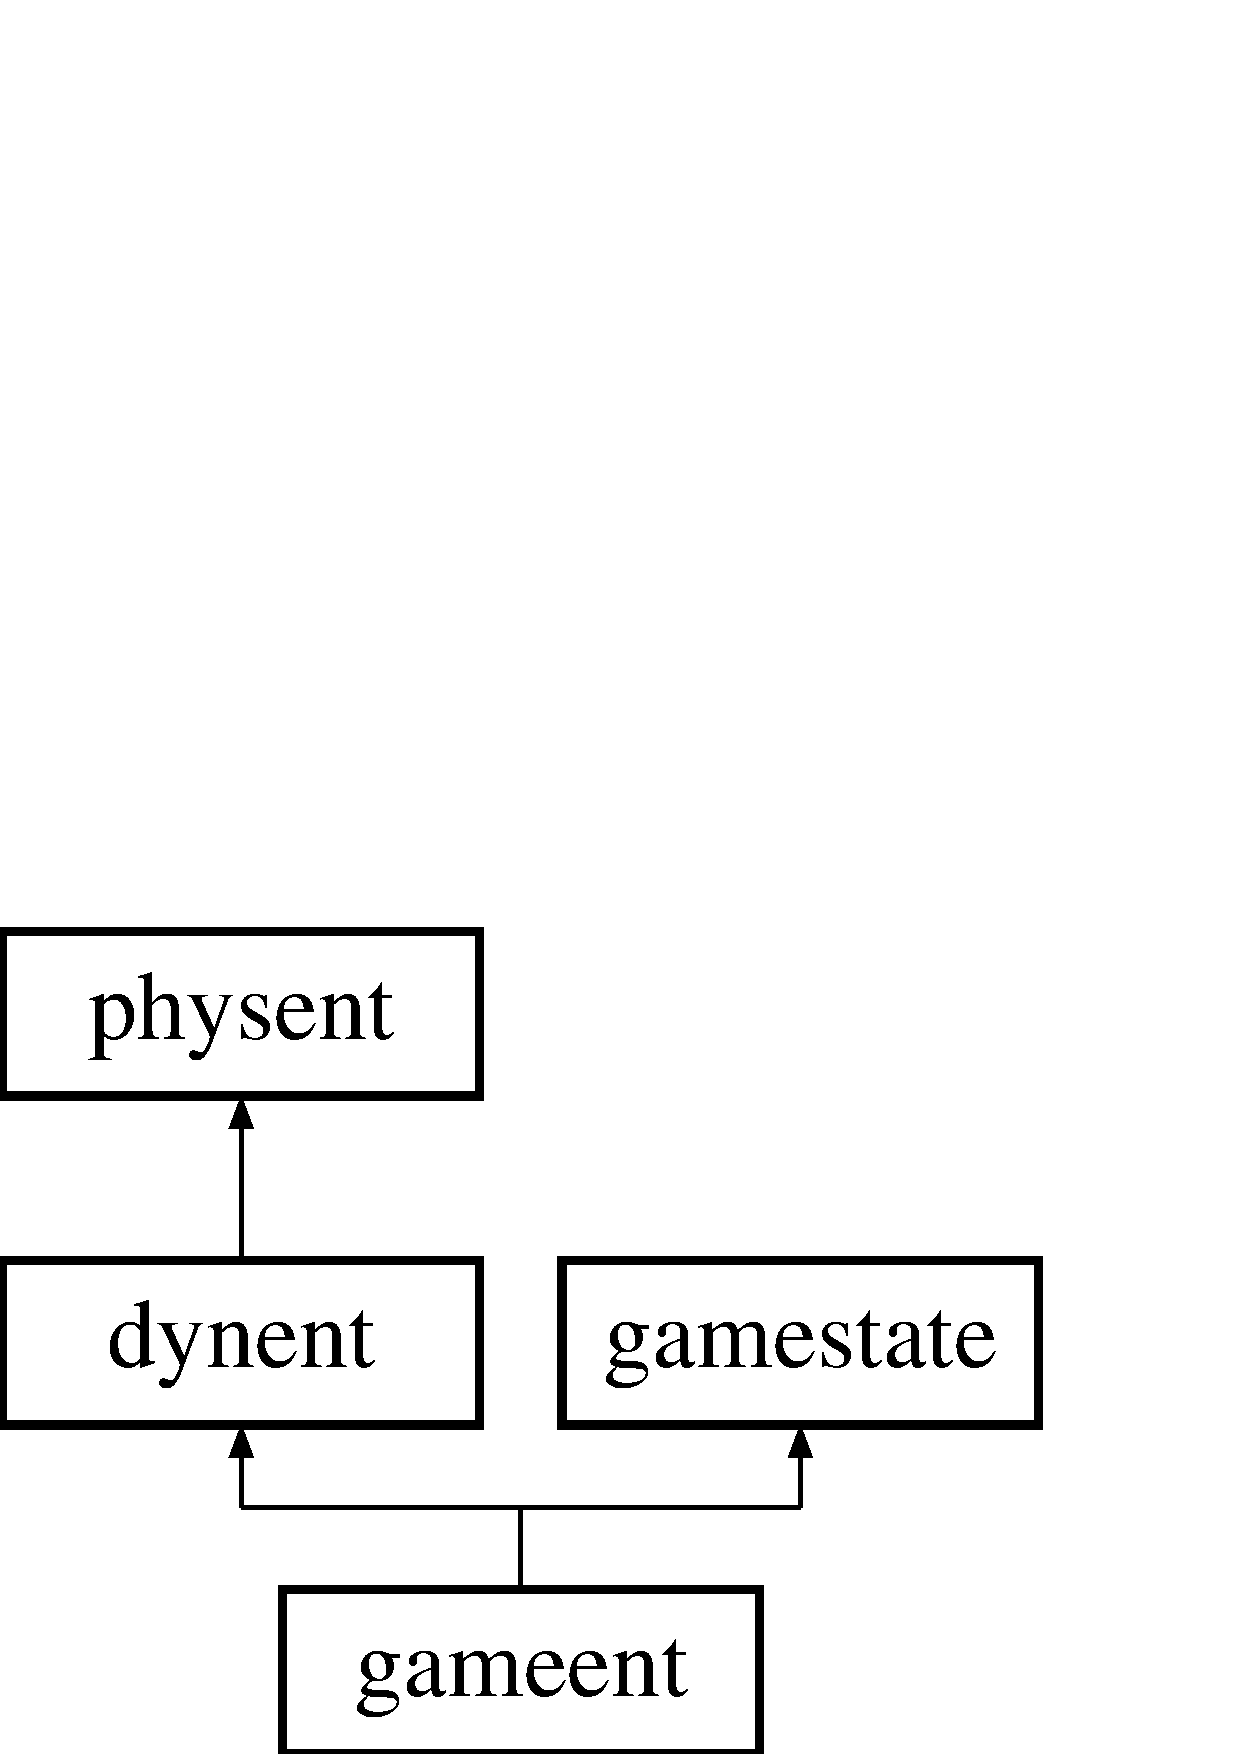
\includegraphics[height=3.000000cm]{structgameent}
\end{center}
\end{figure}
\subsection*{Public Member Functions}
\begin{DoxyCompactItemize}
\item 
\mbox{\Hypertarget{structgameent_a4f8f44b2ea1dad8492834cc90ba46c8a}\label{structgameent_a4f8f44b2ea1dad8492834cc90ba46c8a}} 
void {\bfseries hitpush} (int damage, const \hyperlink{structvec}{vec} \&dir, \hyperlink{structgameent}{gameent} $\ast$actor, int atk)
\item 
\mbox{\Hypertarget{structgameent_aca144489558ae47e1ace5a4f83bacd6e}\label{structgameent_aca144489558ae47e1ace5a4f83bacd6e}} 
void {\bfseries respawn} ()
\item 
\mbox{\Hypertarget{structgameent_a0522825681e5157265754dcc230100cd}\label{structgameent_a0522825681e5157265754dcc230100cd}} 
void {\bfseries startgame} ()
\end{DoxyCompactItemize}
\subsection*{Public Attributes}
\begin{DoxyCompactItemize}
\item 
\mbox{\Hypertarget{structgameent_ad338aecc1088ca1c6a97bb004dfbb055}\label{structgameent_ad338aecc1088ca1c6a97bb004dfbb055}} 
int {\bfseries weight}
\item 
\mbox{\Hypertarget{structgameent_a6b54f9bf672accb4d209a70a63fc5d82}\label{structgameent_a6b54f9bf672accb4d209a70a63fc5d82}} 
int {\bfseries clientnum}
\item 
\mbox{\Hypertarget{structgameent_a468c7c1af4313184f1bf1c840e4026ce}\label{structgameent_a468c7c1af4313184f1bf1c840e4026ce}} 
int {\bfseries privilege}
\item 
\mbox{\Hypertarget{structgameent_a4df30efe36f19779eed269a1f7b47058}\label{structgameent_a4df30efe36f19779eed269a1f7b47058}} 
int {\bfseries lastupdate}
\item 
\mbox{\Hypertarget{structgameent_a311761afd74c0174a680e10bcbb06060}\label{structgameent_a311761afd74c0174a680e10bcbb06060}} 
int {\bfseries plag}
\item 
\mbox{\Hypertarget{structgameent_afbbe5919f65c6ad4bad647b89258a30a}\label{structgameent_afbbe5919f65c6ad4bad647b89258a30a}} 
int {\bfseries ping}
\item 
\mbox{\Hypertarget{structgameent_a105952a1fe0753d68008231127fc9a36}\label{structgameent_a105952a1fe0753d68008231127fc9a36}} 
int {\bfseries lifesequence}
\item 
\mbox{\Hypertarget{structgameent_a5313deae369e402e8d2a6944c82a23ab}\label{structgameent_a5313deae369e402e8d2a6944c82a23ab}} 
int {\bfseries respawned}
\item 
\mbox{\Hypertarget{structgameent_a3a9a3aa1e037dbe8dd4b1a33969b5e63}\label{structgameent_a3a9a3aa1e037dbe8dd4b1a33969b5e63}} 
int {\bfseries suicided}
\item 
\mbox{\Hypertarget{structgameent_a7db416cf9b16316656aea421c1abc34f}\label{structgameent_a7db416cf9b16316656aea421c1abc34f}} 
int {\bfseries lastpain}
\item 
\mbox{\Hypertarget{structgameent_a95fa83e7f7894db30fe8e690c4ca9edf}\label{structgameent_a95fa83e7f7894db30fe8e690c4ca9edf}} 
int {\bfseries lastaction}
\item 
\mbox{\Hypertarget{structgameent_ac01a0135b6f96ed65357221107c64d4e}\label{structgameent_ac01a0135b6f96ed65357221107c64d4e}} 
int {\bfseries lastattack}
\item 
\mbox{\Hypertarget{structgameent_a45112ee1aebb30e02aae34e1d3dc954a}\label{structgameent_a45112ee1aebb30e02aae34e1d3dc954a}} 
int {\bfseries attacking}
\item 
\mbox{\Hypertarget{structgameent_a77da220f93cfcf2fc2a14f56f4804546}\label{structgameent_a77da220f93cfcf2fc2a14f56f4804546}} 
int {\bfseries lasttaunt}
\item 
\mbox{\Hypertarget{structgameent_a4c7729d77d3e332f1aede0359acbff1a}\label{structgameent_a4c7729d77d3e332f1aede0359acbff1a}} 
int {\bfseries lastpickup}
\item 
\mbox{\Hypertarget{structgameent_a16f2b37f7da71c3f033ff790a98817bf}\label{structgameent_a16f2b37f7da71c3f033ff790a98817bf}} 
int {\bfseries lastpickupmillis}
\item 
\mbox{\Hypertarget{structgameent_a29158de462c339c7e3e4d26aedff7b52}\label{structgameent_a29158de462c339c7e3e4d26aedff7b52}} 
int {\bfseries flagpickup}
\item 
\mbox{\Hypertarget{structgameent_abdb3faca2b455b49b98a43a45811b6ca}\label{structgameent_abdb3faca2b455b49b98a43a45811b6ca}} 
int {\bfseries frags}
\item 
\mbox{\Hypertarget{structgameent_a1e2216488428b588d3446603892bca49}\label{structgameent_a1e2216488428b588d3446603892bca49}} 
int {\bfseries flags}
\item 
\mbox{\Hypertarget{structgameent_a496e1add24bb5510c937aea198a60328}\label{structgameent_a496e1add24bb5510c937aea198a60328}} 
int {\bfseries deaths}
\item 
\mbox{\Hypertarget{structgameent_a183e53684b8bc57de60523c25ef37851}\label{structgameent_a183e53684b8bc57de60523c25ef37851}} 
int {\bfseries totaldamage}
\item 
\mbox{\Hypertarget{structgameent_aaa6e5661bb6de7a31aadc8150e4e4a57}\label{structgameent_aaa6e5661bb6de7a31aadc8150e4e4a57}} 
int {\bfseries totalshots}
\item 
\mbox{\Hypertarget{structgameent_ae8be75f40358acfc1af8f602ecd69eba}\label{structgameent_ae8be75f40358acfc1af8f602ecd69eba}} 
\hyperlink{structeditinfo}{editinfo} $\ast$ {\bfseries edit}
\item 
\mbox{\Hypertarget{structgameent_a4018c7780dd9a4192db81386267d4672}\label{structgameent_a4018c7780dd9a4192db81386267d4672}} 
float {\bfseries deltayaw}
\item 
\mbox{\Hypertarget{structgameent_aaebac97d98f5638ac4b90a0dab3ab142}\label{structgameent_aaebac97d98f5638ac4b90a0dab3ab142}} 
float {\bfseries deltapitch}
\item 
\mbox{\Hypertarget{structgameent_a5c9cb65191ceb301ebd2fbb0abfa952c}\label{structgameent_a5c9cb65191ceb301ebd2fbb0abfa952c}} 
float {\bfseries deltaroll}
\item 
\mbox{\Hypertarget{structgameent_a382a97bcced87e53e1b4a94161de42a5}\label{structgameent_a382a97bcced87e53e1b4a94161de42a5}} 
float {\bfseries newyaw}
\item 
\mbox{\Hypertarget{structgameent_aa92bf022c8856fc9f7c31596193c3eb2}\label{structgameent_aa92bf022c8856fc9f7c31596193c3eb2}} 
float {\bfseries newpitch}
\item 
\mbox{\Hypertarget{structgameent_a99797cfdf3e45e7efa59265171da1c78}\label{structgameent_a99797cfdf3e45e7efa59265171da1c78}} 
float {\bfseries newroll}
\item 
\mbox{\Hypertarget{structgameent_a4541e881665dcb944f305c5563c05548}\label{structgameent_a4541e881665dcb944f305c5563c05548}} 
int {\bfseries smoothmillis}
\item 
\mbox{\Hypertarget{structgameent_a4201601798dd0365f60649b2a88ce82a}\label{structgameent_a4201601798dd0365f60649b2a88ce82a}} 
cubestr {\bfseries name}
\item 
\mbox{\Hypertarget{structgameent_ab807211f12d9ab794054e830e2be38ee}\label{structgameent_ab807211f12d9ab794054e830e2be38ee}} 
cubestr {\bfseries info}
\item 
\mbox{\Hypertarget{structgameent_ac55bb01225db3cfc0be9e3e3b0f1e15d}\label{structgameent_ac55bb01225db3cfc0be9e3e3b0f1e15d}} 
int {\bfseries team}
\item 
\mbox{\Hypertarget{structgameent_a7e6e372eacba1eaa232cc918aa220f17}\label{structgameent_a7e6e372eacba1eaa232cc918aa220f17}} 
int {\bfseries playermodel}
\item 
\mbox{\Hypertarget{structgameent_a8c4ee596e56b0933f9e3b9321cc2657e}\label{structgameent_a8c4ee596e56b0933f9e3b9321cc2657e}} 
int {\bfseries playercolor}
\item 
\mbox{\Hypertarget{structgameent_a41e549e0b72d9e1fc49c6942e7dc0819}\label{structgameent_a41e549e0b72d9e1fc49c6942e7dc0819}} 
\hyperlink{structai_1_1aiinfo}{ai\+::aiinfo} $\ast$ {\bfseries ai}
\item 
\mbox{\Hypertarget{structgameent_a45c55aa030133a7cccece63bf13005f8}\label{structgameent_a45c55aa030133a7cccece63bf13005f8}} 
int {\bfseries ownernum}
\item 
\mbox{\Hypertarget{structgameent_abb043b1c8e664b30e49868d27e82d77c}\label{structgameent_abb043b1c8e664b30e49868d27e82d77c}} 
int {\bfseries lastnode}
\item 
\mbox{\Hypertarget{structgameent_a78506020c7df87d82d9af3160e3c1442}\label{structgameent_a78506020c7df87d82d9af3160e3c1442}} 
\hyperlink{structvec}{vec} {\bfseries muzzle}
\end{DoxyCompactItemize}


The documentation for this struct was generated from the following file\+:\begin{DoxyCompactItemize}
\item 
H\+:/\+Rival\+Engine/\+Rival\+\_\+\+Game\+\_\+\+Engine\+\_\+\+G\+I\+T/\+Rival3dengine/source/game/game.\+h\end{DoxyCompactItemize}

\hypertarget{structgameentity}{}\section{gameentity Struct Reference}
\label{structgameentity}\index{gameentity@{gameentity}}
Inheritance diagram for gameentity\+:\begin{figure}[H]
\begin{center}
\leavevmode
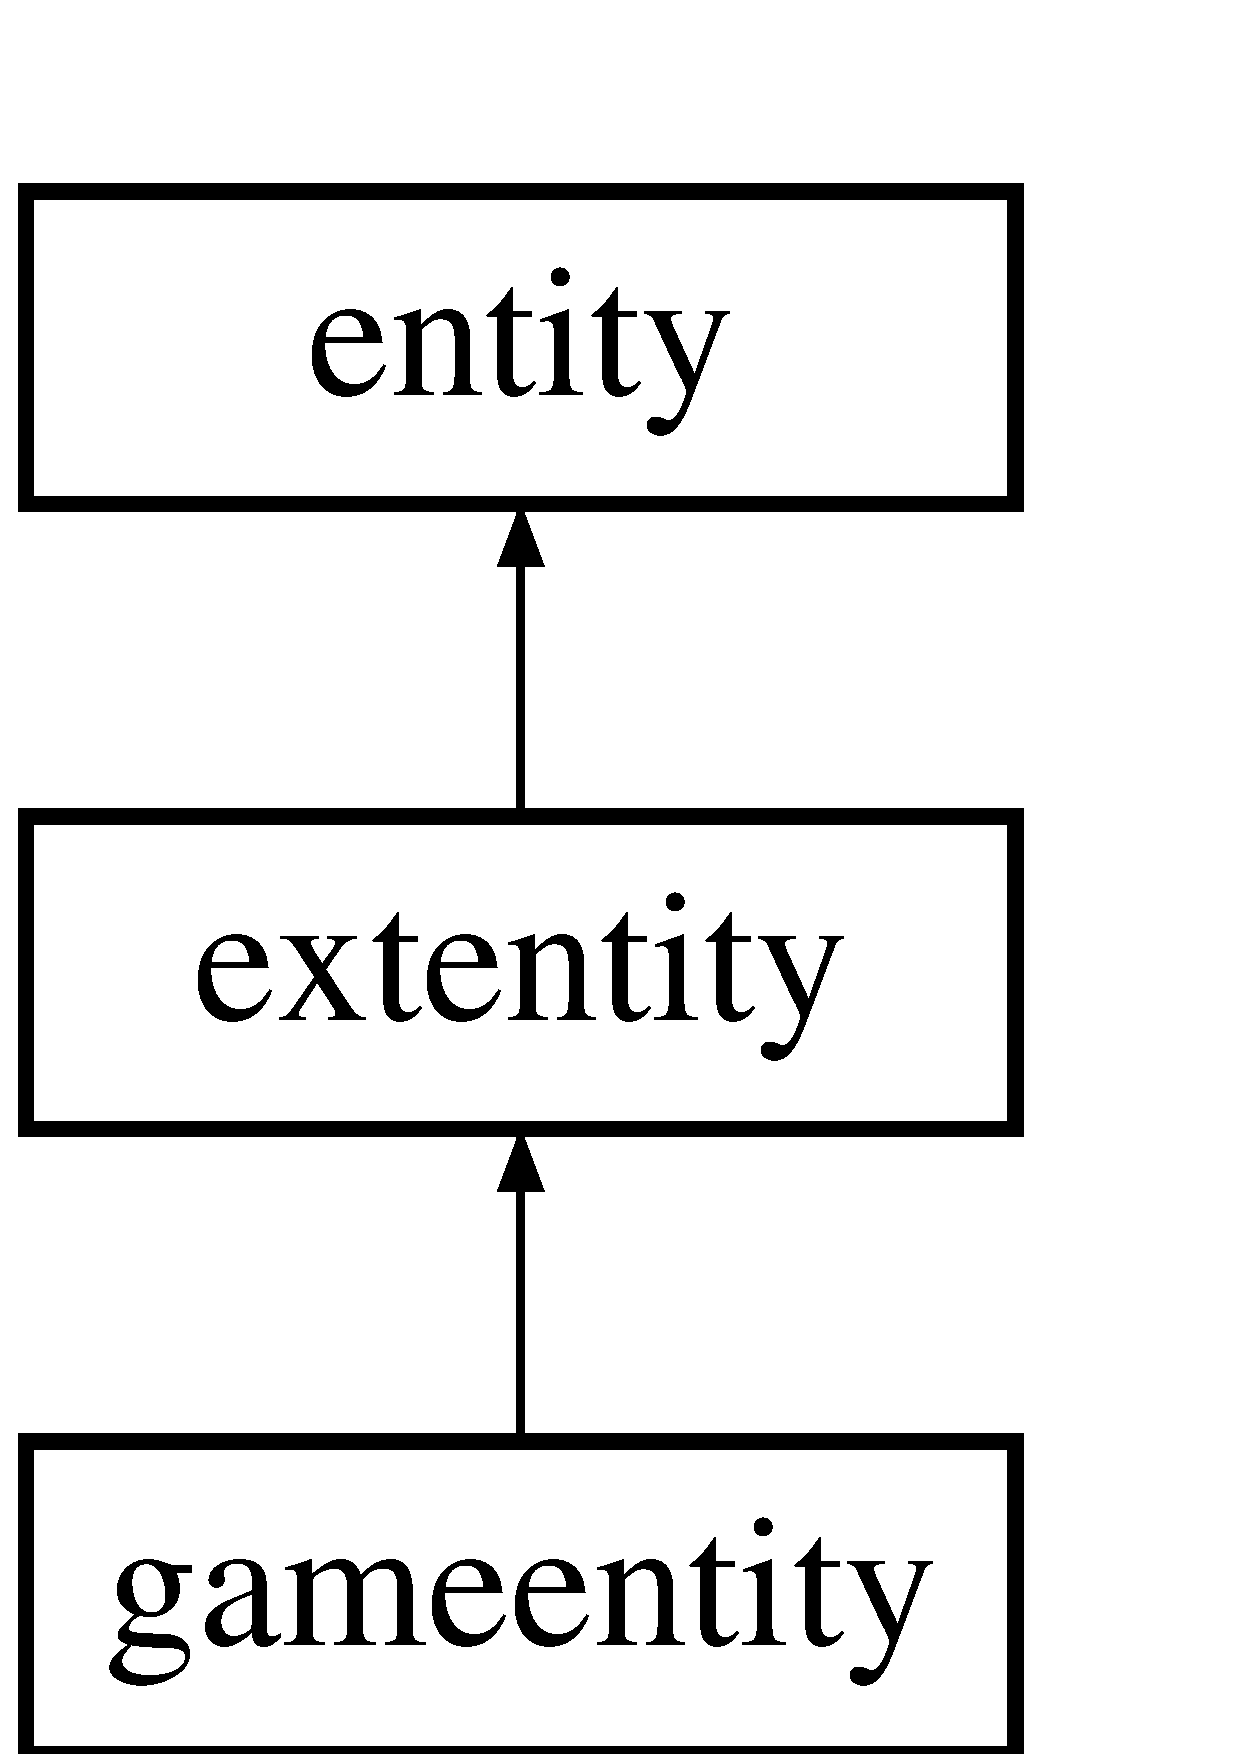
\includegraphics[height=3.000000cm]{structgameentity}
\end{center}
\end{figure}
\subsection*{Public Attributes}
\begin{DoxyCompactItemize}
\item 
\mbox{\Hypertarget{structgameentity_a3695aeb4f84784f035661b41aa76fcbd}\label{structgameentity_a3695aeb4f84784f035661b41aa76fcbd}} 
int {\bfseries triggerstate}
\item 
\mbox{\Hypertarget{structgameentity_ae7dbfea7e0f3e1c10b7744f5153b4fd4}\label{structgameentity_ae7dbfea7e0f3e1c10b7744f5153b4fd4}} 
int {\bfseries lasttrigger}
\end{DoxyCompactItemize}
\subsection*{Additional Inherited Members}


The documentation for this struct was generated from the following file\+:\begin{DoxyCompactItemize}
\item 
H\+:/\+Rival\+Engine/\+Rival\+\_\+\+Game\+\_\+\+Engine\+\_\+\+G\+I\+T/\+Rival3dengine/source/game/game.\+h\end{DoxyCompactItemize}

\hypertarget{structserver_1_1gameevent}{}\section{server\+:\+:gameevent Struct Reference}
\label{structserver_1_1gameevent}\index{server\+::gameevent@{server\+::gameevent}}
Inheritance diagram for server\+:\+:gameevent\+:\begin{figure}[H]
\begin{center}
\leavevmode
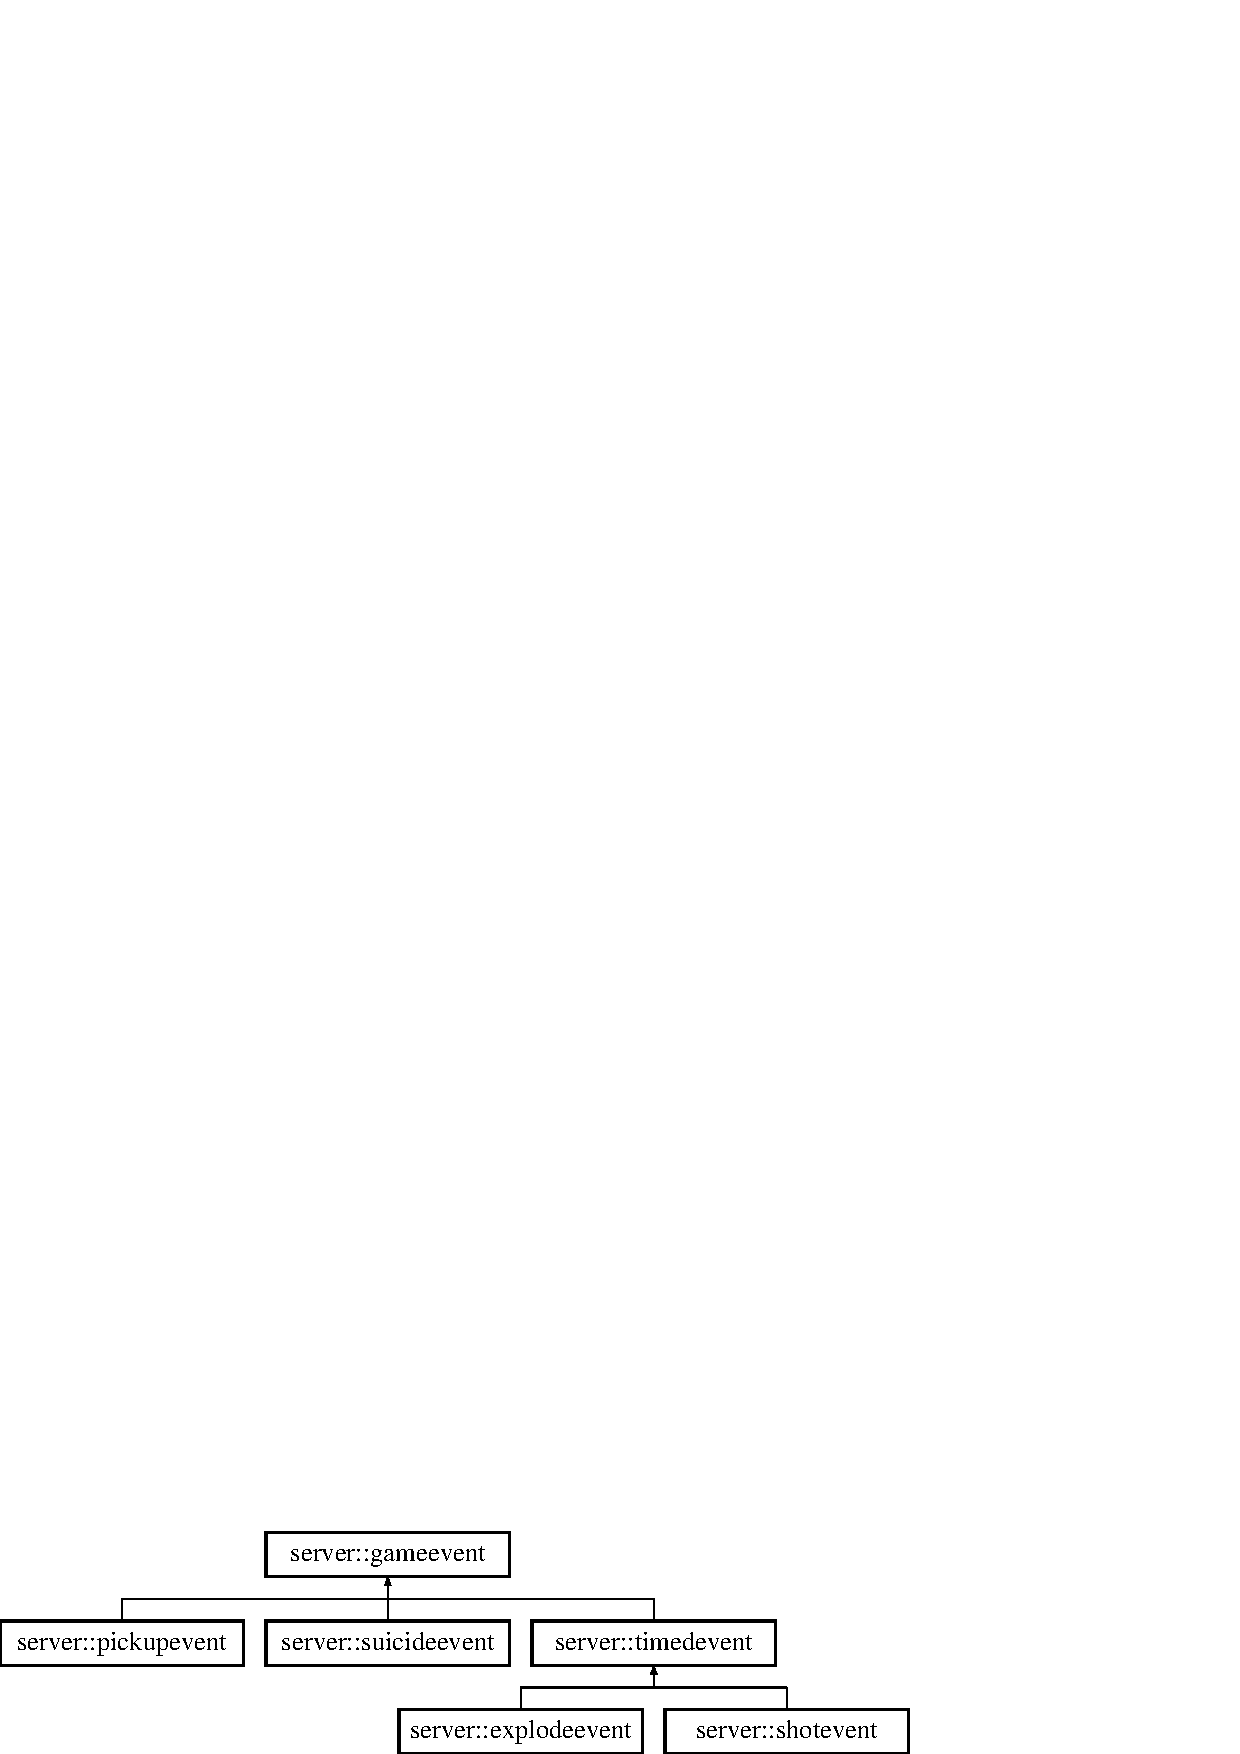
\includegraphics[height=3.000000cm]{structserver_1_1gameevent}
\end{center}
\end{figure}
\subsection*{Public Member Functions}
\begin{DoxyCompactItemize}
\item 
\mbox{\Hypertarget{structserver_1_1gameevent_ac0a663a9bb2fdb51af36be3325338554}\label{structserver_1_1gameevent_ac0a663a9bb2fdb51af36be3325338554}} 
virtual bool {\bfseries flush} (\hyperlink{structserver_1_1clientinfo}{clientinfo} $\ast$ci, int fmillis)
\item 
\mbox{\Hypertarget{structserver_1_1gameevent_afa56069ed44707cd379e3680ddb55666}\label{structserver_1_1gameevent_afa56069ed44707cd379e3680ddb55666}} 
virtual void {\bfseries process} (\hyperlink{structserver_1_1clientinfo}{clientinfo} $\ast$ci)
\item 
\mbox{\Hypertarget{structserver_1_1gameevent_a488316582bf627973ef7bfe72a17752c}\label{structserver_1_1gameevent_a488316582bf627973ef7bfe72a17752c}} 
virtual bool {\bfseries keepable} () const
\end{DoxyCompactItemize}


The documentation for this struct was generated from the following file\+:\begin{DoxyCompactItemize}
\item 
H\+:/\+Rival\+Engine/\+Rival\+\_\+\+Game\+\_\+\+Engine\+\_\+\+G\+I\+T/\+Rival3dengine/source/game/server.\+cpp\end{DoxyCompactItemize}

\hypertarget{structentities_1_1gamemode}{}\section{entities\+:\+:gamemode Struct Reference}
\label{structentities_1_1gamemode}\index{entities\+::gamemode@{entities\+::gamemode}}


The documentation for this struct was generated from the following file\+:\begin{DoxyCompactItemize}
\item 
H\+:/\+Rival\+Engine/\+Rival\+\_\+\+Game\+\_\+\+Engine\+\_\+\+G\+I\+T/\+Rival3dengine/source/game/game.\+h\end{DoxyCompactItemize}

\hypertarget{structgameserver}{}\section{gameserver Struct Reference}
\label{structgameserver}\index{gameserver@{gameserver}}
\subsection*{Public Attributes}
\begin{DoxyCompactItemize}
\item 
\mbox{\Hypertarget{structgameserver_ac7448414c74412c23111d2adbe3cff00}\label{structgameserver_ac7448414c74412c23111d2adbe3cff00}} 
E\+Net\+Address {\bfseries address}
\item 
\mbox{\Hypertarget{structgameserver_a9bf2978b3a76a4f5427416cdac66d267}\label{structgameserver_a9bf2978b3a76a4f5427416cdac66d267}} 
string {\bfseries ip}
\item 
\mbox{\Hypertarget{structgameserver_a3b1baafd52dc6239aed4b865a04f28be}\label{structgameserver_a3b1baafd52dc6239aed4b865a04f28be}} 
int {\bfseries port}
\item 
\mbox{\Hypertarget{structgameserver_ab1ba9f229809ae585b1ccac91a5b533e}\label{structgameserver_ab1ba9f229809ae585b1ccac91a5b533e}} 
int {\bfseries numpings}
\item 
\mbox{\Hypertarget{structgameserver_ac77872cecf83320fd3b2515d2797971b}\label{structgameserver_ac77872cecf83320fd3b2515d2797971b}} 
enet\+\_\+uint32 {\bfseries lastping}
\item 
\mbox{\Hypertarget{structgameserver_aecd4c7c26ba333f853093c60c6bc334d}\label{structgameserver_aecd4c7c26ba333f853093c60c6bc334d}} 
enet\+\_\+uint32 {\bfseries lastpong}
\end{DoxyCompactItemize}


The documentation for this struct was generated from the following file\+:\begin{DoxyCompactItemize}
\item 
H\+:/\+Rival\+Engine/\+Rival\+\_\+\+Game\+\_\+\+Engine\+\_\+\+G\+I\+T/\+Rival3dengine/source/engine/master.\+cpp\end{DoxyCompactItemize}

\hypertarget{structgamestate}{}\section{gamestate Struct Reference}
\label{structgamestate}\index{gamestate@{gamestate}}
Inheritance diagram for gamestate\+:\begin{figure}[H]
\begin{center}
\leavevmode
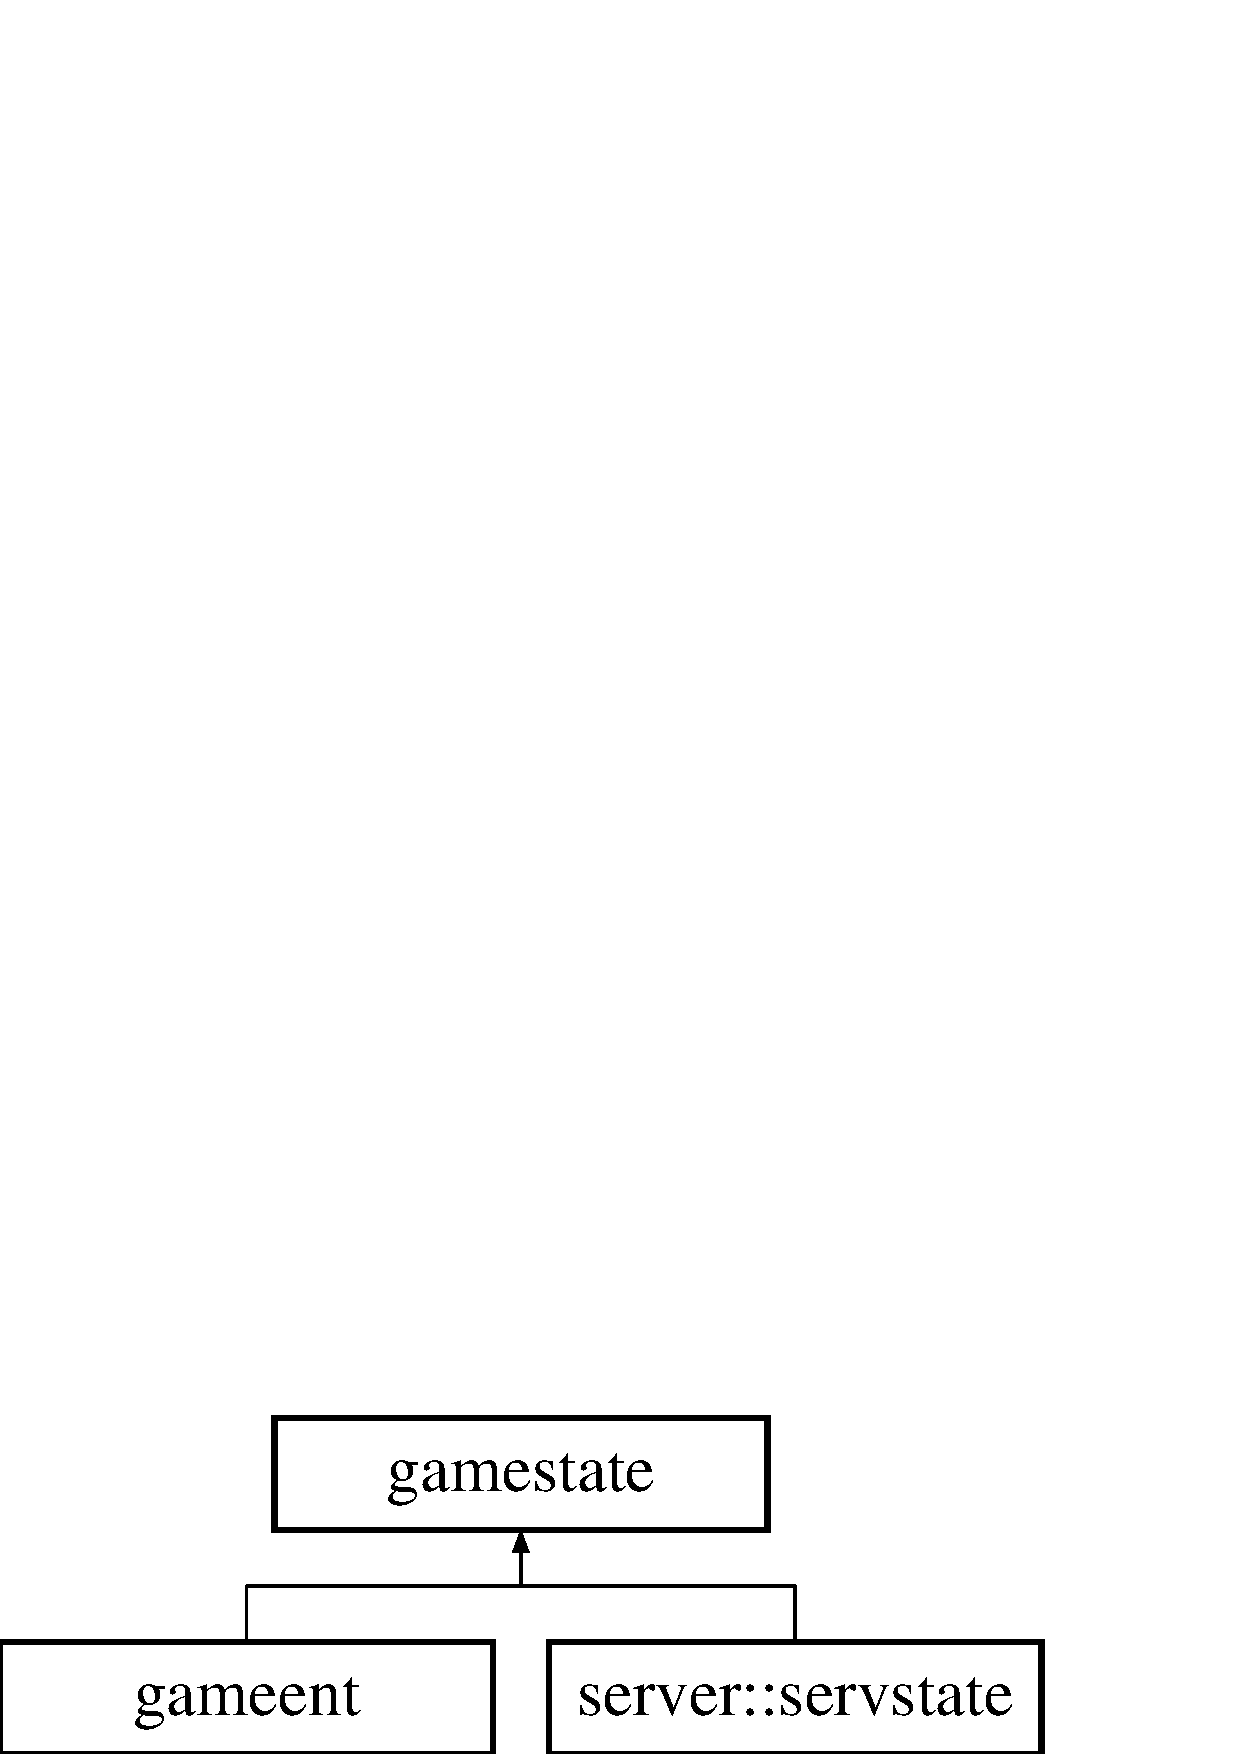
\includegraphics[height=2.000000cm]{structgamestate}
\end{center}
\end{figure}
\subsection*{Public Member Functions}
\begin{DoxyCompactItemize}
\item 
\mbox{\Hypertarget{structgamestate_a13710cb67f9834b852ff4d3a56766e43}\label{structgamestate_a13710cb67f9834b852ff4d3a56766e43}} 
bool {\bfseries canpickup} (int type)
\item 
\mbox{\Hypertarget{structgamestate_a43007bc8af87aa01f76d3673280bbb47}\label{structgamestate_a43007bc8af87aa01f76d3673280bbb47}} 
void {\bfseries pickup} (int type)
\item 
\mbox{\Hypertarget{structgamestate_a47090211e18fb02c7316712d9e5c57ea}\label{structgamestate_a47090211e18fb02c7316712d9e5c57ea}} 
void {\bfseries respawn} ()
\item 
\mbox{\Hypertarget{structgamestate_a8172ba069d1f551576a55f6ff36a9dd8}\label{structgamestate_a8172ba069d1f551576a55f6ff36a9dd8}} 
void {\bfseries spawnstate} (int gamemode)
\item 
\mbox{\Hypertarget{structgamestate_a71220d27f9ae980828d3bdb8cdb6b39e}\label{structgamestate_a71220d27f9ae980828d3bdb8cdb6b39e}} 
int {\bfseries dodamage} (int damage)
\item 
\mbox{\Hypertarget{structgamestate_ae886b4c6a9a222f79357a5f656f2d9f2}\label{structgamestate_ae886b4c6a9a222f79357a5f656f2d9f2}} 
int {\bfseries hasammo} (int gun, int exclude=-\/1)
\end{DoxyCompactItemize}
\subsection*{Public Attributes}
\begin{DoxyCompactItemize}
\item 
\mbox{\Hypertarget{structgamestate_a4419b76fa9ce49784b580d42b2f4db2c}\label{structgamestate_a4419b76fa9ce49784b580d42b2f4db2c}} 
int {\bfseries health}
\item 
\mbox{\Hypertarget{structgamestate_a6fefe845b162b52a286c542422e8317a}\label{structgamestate_a6fefe845b162b52a286c542422e8317a}} 
int {\bfseries maxhealth}
\item 
\mbox{\Hypertarget{structgamestate_a61a239a37419bb354cc407a7f4aafcbc}\label{structgamestate_a61a239a37419bb354cc407a7f4aafcbc}} 
int {\bfseries gunselect}
\item 
\mbox{\Hypertarget{structgamestate_a07fc227a67228ad47d9db8477b6212d3}\label{structgamestate_a07fc227a67228ad47d9db8477b6212d3}} 
int {\bfseries gunwait}
\item 
\mbox{\Hypertarget{structgamestate_a07c2af3e09994ee8bbbcd75714348235}\label{structgamestate_a07c2af3e09994ee8bbbcd75714348235}} 
int {\bfseries ammo} \mbox{[}N\+U\+M\+G\+U\+NS\mbox{]}
\item 
\mbox{\Hypertarget{structgamestate_aa08f0b162cf7bf5b9b9ac469f637a9f3}\label{structgamestate_aa08f0b162cf7bf5b9b9ac469f637a9f3}} 
int {\bfseries aitype}
\item 
\mbox{\Hypertarget{structgamestate_a67b62dbd716253e15e7ec31b28ffb595}\label{structgamestate_a67b62dbd716253e15e7ec31b28ffb595}} 
int {\bfseries skill}
\end{DoxyCompactItemize}


The documentation for this struct was generated from the following file\+:\begin{DoxyCompactItemize}
\item 
H\+:/\+Rival\+Engine/\+Rival\+\_\+\+Game\+\_\+\+Engine\+\_\+\+G\+I\+T/\+Rival3dengine/source/game/game.\+h\end{DoxyCompactItemize}

\hypertarget{structgeombatch}{}\section{geombatch Struct Reference}
\label{structgeombatch}\index{geombatch@{geombatch}}
\subsection*{Public Member Functions}
\begin{DoxyCompactItemize}
\item 
\mbox{\Hypertarget{structgeombatch_ac75f7955c15112f6632167b4df56b155}\label{structgeombatch_ac75f7955c15112f6632167b4df56b155}} 
{\bfseries geombatch} (const \hyperlink{structelementset}{elementset} \&es, int offset, \hyperlink{structvtxarray}{vtxarray} $\ast$va)
\item 
\mbox{\Hypertarget{structgeombatch_a2f14476a7aec8444433611fa9f1a87d9}\label{structgeombatch_a2f14476a7aec8444433611fa9f1a87d9}} 
int {\bfseries compare} (const \hyperlink{structgeombatch}{geombatch} \&b) const
\end{DoxyCompactItemize}
\subsection*{Public Attributes}
\begin{DoxyCompactItemize}
\item 
\mbox{\Hypertarget{structgeombatch_acee6e8d29c3bd980ecd615f757bdb3f2}\label{structgeombatch_acee6e8d29c3bd980ecd615f757bdb3f2}} 
const \hyperlink{structelementset}{elementset} \& {\bfseries es}
\item 
\mbox{\Hypertarget{structgeombatch_ad14b264f35d6b77f9285bfb15f398e1c}\label{structgeombatch_ad14b264f35d6b77f9285bfb15f398e1c}} 
\hyperlink{struct_v_slot}{V\+Slot} \& {\bfseries vslot}
\item 
\mbox{\Hypertarget{structgeombatch_abaf812ca1329016141bca1570636fd03}\label{structgeombatch_abaf812ca1329016141bca1570636fd03}} 
int {\bfseries offset}
\item 
\mbox{\Hypertarget{structgeombatch_a8645392b8037d035b15dffb249f0225d}\label{structgeombatch_a8645392b8037d035b15dffb249f0225d}} 
\hyperlink{structvtxarray}{vtxarray} $\ast$ {\bfseries va}
\item 
\mbox{\Hypertarget{structgeombatch_a48d19e83c58bc01f4cb9fd65dc5ba896}\label{structgeombatch_a48d19e83c58bc01f4cb9fd65dc5ba896}} 
int {\bfseries next}
\item 
\mbox{\Hypertarget{structgeombatch_a4131dcfaa64e3118af144cbf363833aa}\label{structgeombatch_a4131dcfaa64e3118af144cbf363833aa}} 
int {\bfseries batch}
\end{DoxyCompactItemize}


The documentation for this struct was generated from the following file\+:\begin{DoxyCompactItemize}
\item 
H\+:/\+Rival\+Engine/\+Rival\+\_\+\+Game\+\_\+\+Engine\+\_\+\+G\+I\+T/\+Rival3dengine/source/engine/renderva.\+cpp\end{DoxyCompactItemize}

\hypertarget{structgfield}{}\section{gfield Struct Reference}
\label{structgfield}\index{gfield@{gfield}}
Inheritance diagram for gfield\+:\begin{figure}[H]
\begin{center}
\leavevmode
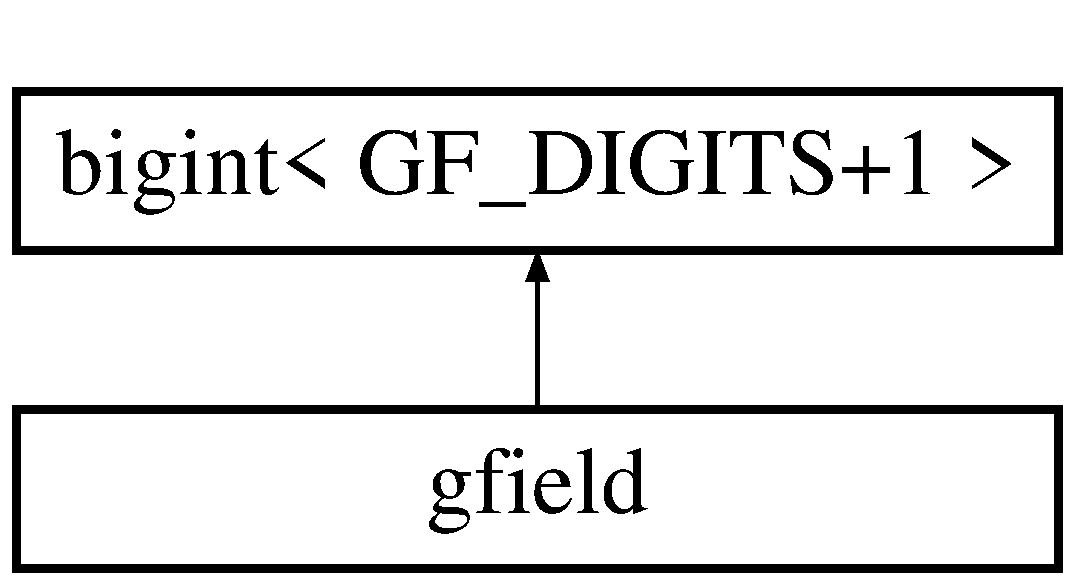
\includegraphics[height=2.000000cm]{structgfield}
\end{center}
\end{figure}
\subsection*{Public Member Functions}
\begin{DoxyCompactItemize}
\item 
\mbox{\Hypertarget{structgfield_a7f4b59d395ef7a10002015cb14a18404}\label{structgfield_a7f4b59d395ef7a10002015cb14a18404}} 
{\bfseries gfield} (digit n)
\item 
\mbox{\Hypertarget{structgfield_a284ffd2e552aa1b16ab8a497a2459819}\label{structgfield_a284ffd2e552aa1b16ab8a497a2459819}} 
{\bfseries gfield} (const char $\ast$s)
\item 
\mbox{\Hypertarget{structgfield_a3172d0ca3de822faeefc836387518840}\label{structgfield_a3172d0ca3de822faeefc836387518840}} 
{\footnotesize template$<$int Y\+\_\+\+D\+I\+G\+I\+TS$>$ }\\{\bfseries gfield} (const \hyperlink{structbigint}{bigint}$<$ Y\+\_\+\+D\+I\+G\+I\+TS $>$ \&y)
\item 
\mbox{\Hypertarget{structgfield_a9b0f4685fac80185136975c7db38ff1f}\label{structgfield_a9b0f4685fac80185136975c7db38ff1f}} 
{\footnotesize template$<$int Y\+\_\+\+D\+I\+G\+I\+TS$>$ }\\\hyperlink{structgfield}{gfield} \& {\bfseries operator=} (const \hyperlink{structbigint}{bigint}$<$ Y\+\_\+\+D\+I\+G\+I\+TS $>$ \&y)
\item 
\mbox{\Hypertarget{structgfield_ac42fa6dc3ebec3ba7ae9143e363e8c06}\label{structgfield_ac42fa6dc3ebec3ba7ae9143e363e8c06}} 
{\footnotesize template$<$int X\+\_\+\+D\+I\+G\+I\+TS, int Y\+\_\+\+D\+I\+G\+I\+TS$>$ }\\\hyperlink{structgfield}{gfield} \& {\bfseries add} (const \hyperlink{structbigint}{bigint}$<$ X\+\_\+\+D\+I\+G\+I\+TS $>$ \&x, const \hyperlink{structbigint}{bigint}$<$ Y\+\_\+\+D\+I\+G\+I\+TS $>$ \&y)
\item 
\mbox{\Hypertarget{structgfield_a421446ca3f9e995438f49769ad28d58d}\label{structgfield_a421446ca3f9e995438f49769ad28d58d}} 
{\footnotesize template$<$int Y\+\_\+\+D\+I\+G\+I\+TS$>$ }\\\hyperlink{structgfield}{gfield} \& {\bfseries add} (const \hyperlink{structbigint}{bigint}$<$ Y\+\_\+\+D\+I\+G\+I\+TS $>$ \&y)
\item 
\mbox{\Hypertarget{structgfield_a11934c0293bd72b5010d7bd2b8f8a679}\label{structgfield_a11934c0293bd72b5010d7bd2b8f8a679}} 
{\footnotesize template$<$int X\+\_\+\+D\+I\+G\+I\+TS$>$ }\\\hyperlink{structgfield}{gfield} \& {\bfseries mul2} (const \hyperlink{structbigint}{bigint}$<$ X\+\_\+\+D\+I\+G\+I\+TS $>$ \&x)
\item 
\mbox{\Hypertarget{structgfield_a4b1eb43a6d41cd9b405f19827965a3fb}\label{structgfield_a4b1eb43a6d41cd9b405f19827965a3fb}} 
\hyperlink{structgfield}{gfield} \& {\bfseries mul2} ()
\item 
\mbox{\Hypertarget{structgfield_abc7d6d9d3fbc4c2ef13f05ab41e3f1c1}\label{structgfield_abc7d6d9d3fbc4c2ef13f05ab41e3f1c1}} 
\hyperlink{structgfield}{gfield} \& {\bfseries div2} ()
\item 
\mbox{\Hypertarget{structgfield_a7b28f9e10bd7425d2ccf855cde3daedb}\label{structgfield_a7b28f9e10bd7425d2ccf855cde3daedb}} 
{\footnotesize template$<$int X\+\_\+\+D\+I\+G\+I\+TS, int Y\+\_\+\+D\+I\+G\+I\+TS$>$ }\\\hyperlink{structgfield}{gfield} \& {\bfseries sub} (const \hyperlink{structbigint}{bigint}$<$ X\+\_\+\+D\+I\+G\+I\+TS $>$ \&x, const \hyperlink{structbigint}{bigint}$<$ Y\+\_\+\+D\+I\+G\+I\+TS $>$ \&y)
\item 
\mbox{\Hypertarget{structgfield_a60e81a7e630ccbd0367b20d879d662ab}\label{structgfield_a60e81a7e630ccbd0367b20d879d662ab}} 
{\footnotesize template$<$int Y\+\_\+\+D\+I\+G\+I\+TS$>$ }\\\hyperlink{structgfield}{gfield} \& {\bfseries sub} (const \hyperlink{structbigint}{bigint}$<$ Y\+\_\+\+D\+I\+G\+I\+TS $>$ \&y)
\item 
\mbox{\Hypertarget{structgfield_a1813a78e8ffda06a084c66c8fada2bbf}\label{structgfield_a1813a78e8ffda06a084c66c8fada2bbf}} 
{\footnotesize template$<$int X\+\_\+\+D\+I\+G\+I\+TS$>$ }\\\hyperlink{structgfield}{gfield} \& {\bfseries neg} (const \hyperlink{structbigint}{bigint}$<$ X\+\_\+\+D\+I\+G\+I\+TS $>$ \&x)
\item 
\mbox{\Hypertarget{structgfield_a80de574023c5397b3764642eb40d5b2b}\label{structgfield_a80de574023c5397b3764642eb40d5b2b}} 
\hyperlink{structgfield}{gfield} \& {\bfseries neg} ()
\item 
\mbox{\Hypertarget{structgfield_aa5bd3792b7eddf8b871a249e3bc0db95}\label{structgfield_aa5bd3792b7eddf8b871a249e3bc0db95}} 
{\footnotesize template$<$int X\+\_\+\+D\+I\+G\+I\+TS$>$ }\\\hyperlink{structgfield}{gfield} \& {\bfseries square} (const \hyperlink{structbigint}{bigint}$<$ X\+\_\+\+D\+I\+G\+I\+TS $>$ \&x)
\item 
\mbox{\Hypertarget{structgfield_a61ec85b051991f5fa9cbfca68055aa12}\label{structgfield_a61ec85b051991f5fa9cbfca68055aa12}} 
\hyperlink{structgfield}{gfield} \& {\bfseries square} ()
\item 
\mbox{\Hypertarget{structgfield_a77a81289eedc79b01a32bfe2e8fa131b}\label{structgfield_a77a81289eedc79b01a32bfe2e8fa131b}} 
{\footnotesize template$<$int X\+\_\+\+D\+I\+G\+I\+TS, int Y\+\_\+\+D\+I\+G\+I\+TS$>$ }\\\hyperlink{structgfield}{gfield} \& {\bfseries mul} (const \hyperlink{structbigint}{bigint}$<$ X\+\_\+\+D\+I\+G\+I\+TS $>$ \&x, const \hyperlink{structbigint}{bigint}$<$ Y\+\_\+\+D\+I\+G\+I\+TS $>$ \&y)
\item 
\mbox{\Hypertarget{structgfield_af5cb4fb548dd14324f350c90d549f461}\label{structgfield_af5cb4fb548dd14324f350c90d549f461}} 
{\footnotesize template$<$int Y\+\_\+\+D\+I\+G\+I\+TS$>$ }\\\hyperlink{structgfield}{gfield} \& {\bfseries mul} (const \hyperlink{structbigint}{bigint}$<$ Y\+\_\+\+D\+I\+G\+I\+TS $>$ \&y)
\item 
\mbox{\Hypertarget{structgfield_ac0d0507456fbaa1525e4383532316127}\label{structgfield_ac0d0507456fbaa1525e4383532316127}} 
{\footnotesize template$<$int R\+E\+S\+U\+L\+T\+\_\+\+D\+I\+G\+I\+TS$>$ }\\void {\bfseries reduce} (const \hyperlink{structbigint}{bigint}$<$ R\+E\+S\+U\+L\+T\+\_\+\+D\+I\+G\+I\+TS $>$ \&result)
\item 
\mbox{\Hypertarget{structgfield_afda302aa7c801d63f7dabeb2167a571e}\label{structgfield_afda302aa7c801d63f7dabeb2167a571e}} 
{\footnotesize template$<$int X\+\_\+\+D\+I\+G\+I\+TS, int Y\+\_\+\+D\+I\+G\+I\+TS$>$ }\\\hyperlink{structgfield}{gfield} \& {\bfseries pow} (const \hyperlink{structbigint}{bigint}$<$ X\+\_\+\+D\+I\+G\+I\+TS $>$ \&x, const \hyperlink{structbigint}{bigint}$<$ Y\+\_\+\+D\+I\+G\+I\+TS $>$ \&y)
\item 
\mbox{\Hypertarget{structgfield_aaa66f33709a8e0a9a621b2b4cce55234}\label{structgfield_aaa66f33709a8e0a9a621b2b4cce55234}} 
{\footnotesize template$<$int Y\+\_\+\+D\+I\+G\+I\+TS$>$ }\\\hyperlink{structgfield}{gfield} \& {\bfseries pow} (const \hyperlink{structbigint}{bigint}$<$ Y\+\_\+\+D\+I\+G\+I\+TS $>$ \&y)
\item 
\mbox{\Hypertarget{structgfield_ad0268b80caff487f70f6d56c72a06ef8}\label{structgfield_ad0268b80caff487f70f6d56c72a06ef8}} 
bool {\bfseries invert} (const \hyperlink{structgfield}{gfield} \&x)
\item 
\mbox{\Hypertarget{structgfield_a07a5ebadf9f5ad3fc66855f9ae7bc2db}\label{structgfield_a07a5ebadf9f5ad3fc66855f9ae7bc2db}} 
void {\bfseries invert} ()
\item 
\mbox{\Hypertarget{structgfield_abbce2c607098b7f9a8a6745ede06d6df}\label{structgfield_abbce2c607098b7f9a8a6745ede06d6df}} 
int {\bfseries legendre} () const
\item 
\mbox{\Hypertarget{structgfield_a58b2b4ef05f8c04b007cba51be100116}\label{structgfield_a58b2b4ef05f8c04b007cba51be100116}} 
bool {\bfseries sqrt} (const \hyperlink{structgfield}{gfield} \&x)
\item 
\mbox{\Hypertarget{structgfield_aa322270ecd1e50a7453173794d046ffe}\label{structgfield_aa322270ecd1e50a7453173794d046ffe}} 
bool {\bfseries sqrt} ()
\end{DoxyCompactItemize}
\subsection*{Static Public Member Functions}
\begin{DoxyCompactItemize}
\item 
\mbox{\Hypertarget{structgfield_afd5e9fde28aece20da7029f4fd9c1e81}\label{structgfield_afd5e9fde28aece20da7029f4fd9c1e81}} 
{\footnotesize template$<$int X\+\_\+\+D\+I\+G\+I\+TS$>$ }\\static int {\bfseries legendre} (const \hyperlink{structbigint}{bigint}$<$ X\+\_\+\+D\+I\+G\+I\+TS $>$ \&x)
\end{DoxyCompactItemize}
\subsection*{Static Public Attributes}
\begin{DoxyCompactItemize}
\item 
\mbox{\Hypertarget{structgfield_a46e264cfc2176e14176ae9cfa31dee0e}\label{structgfield_a46e264cfc2176e14176ae9cfa31dee0e}} 
static const \hyperlink{structgfield}{gfield} {\bfseries P}
\end{DoxyCompactItemize}
\subsection*{Additional Inherited Members}


The documentation for this struct was generated from the following file\+:\begin{DoxyCompactItemize}
\item 
H\+:/\+Rival\+Engine/\+Rival\+\_\+\+Game\+\_\+\+Engine\+\_\+\+G\+I\+T/\+Rival3dengine/source/shared/crypto.\+cpp\end{DoxyCompactItemize}

\hypertarget{struct_global_shader_param}{}\section{Global\+Shader\+Param Struct Reference}
\label{struct_global_shader_param}\index{Global\+Shader\+Param@{Global\+Shader\+Param}}
\subsection*{Public Member Functions}
\begin{DoxyCompactItemize}
\item 
\mbox{\Hypertarget{struct_global_shader_param_a9589e84e6b49aebf477d522900abcd9b}\label{struct_global_shader_param_a9589e84e6b49aebf477d522900abcd9b}} 
{\bfseries Global\+Shader\+Param} (const char $\ast$name)
\item 
\mbox{\Hypertarget{struct_global_shader_param_aca4cc5b8c5ba8870c6b16efc8ec8a496}\label{struct_global_shader_param_aca4cc5b8c5ba8870c6b16efc8ec8a496}} 
\hyperlink{struct_global_shader_param_state}{Global\+Shader\+Param\+State} $\ast$ {\bfseries resolve} ()
\item 
\mbox{\Hypertarget{struct_global_shader_param_a3b184cc9892632f420c94db694ad5e1d}\label{struct_global_shader_param_a3b184cc9892632f420c94db694ad5e1d}} 
void {\bfseries setf} (float x=0, float y=0, float z=0, float w=0)
\item 
\mbox{\Hypertarget{struct_global_shader_param_a59d4a5da4a87789b07d3bcdae3595fb8}\label{struct_global_shader_param_a59d4a5da4a87789b07d3bcdae3595fb8}} 
void {\bfseries set} (const \hyperlink{structvec}{vec} \&v, float w=0)
\item 
\mbox{\Hypertarget{struct_global_shader_param_a80b256c46992588d6d5ccafe65856a18}\label{struct_global_shader_param_a80b256c46992588d6d5ccafe65856a18}} 
void {\bfseries set} (const \hyperlink{structvec2}{vec2} \&v, float z=0, float w=0)
\item 
\mbox{\Hypertarget{struct_global_shader_param_aa06845a3e668d37fca071368918accf5}\label{struct_global_shader_param_aa06845a3e668d37fca071368918accf5}} 
void {\bfseries set} (const \hyperlink{structvec4}{vec4} \&v)
\item 
\mbox{\Hypertarget{struct_global_shader_param_a07b68d7e854594062ff1cd678abff846}\label{struct_global_shader_param_a07b68d7e854594062ff1cd678abff846}} 
void {\bfseries set} (const \hyperlink{structplane}{plane} \&p)
\item 
\mbox{\Hypertarget{struct_global_shader_param_a6a1a9575032a473ec5f233b48fa14012}\label{struct_global_shader_param_a6a1a9575032a473ec5f233b48fa14012}} 
void {\bfseries set} (const \hyperlink{structmatrix2}{matrix2} \&m)
\item 
\mbox{\Hypertarget{struct_global_shader_param_a59c61ee3de5dd1de892564027c22dc0e}\label{struct_global_shader_param_a59c61ee3de5dd1de892564027c22dc0e}} 
void {\bfseries set} (const \hyperlink{structmatrix3}{matrix3} \&m)
\item 
\mbox{\Hypertarget{struct_global_shader_param_ac0172bf8e7bf4ab726bc545c27d23018}\label{struct_global_shader_param_ac0172bf8e7bf4ab726bc545c27d23018}} 
void {\bfseries set} (const \hyperlink{structmatrix4}{matrix4} \&m)
\item 
\mbox{\Hypertarget{struct_global_shader_param_abf0e57fb74c837f17476036c073708a8}\label{struct_global_shader_param_abf0e57fb74c837f17476036c073708a8}} 
{\footnotesize template$<$class T $>$ }\\void {\bfseries setv} (const T $\ast$v, int n=1)
\item 
\mbox{\Hypertarget{struct_global_shader_param_a34b6b3838528a7eacd5a120e2f35e1f1}\label{struct_global_shader_param_a34b6b3838528a7eacd5a120e2f35e1f1}} 
void {\bfseries seti} (int x=0, int y=0, int z=0, int w=0)
\item 
\mbox{\Hypertarget{struct_global_shader_param_add582cc877e9f4802ff781c2e9ffd23d}\label{struct_global_shader_param_add582cc877e9f4802ff781c2e9ffd23d}} 
void {\bfseries set} (const \hyperlink{structivec}{ivec} \&v, int w=0)
\item 
\mbox{\Hypertarget{struct_global_shader_param_ad29287e99b91674e0e718fc8450b6732}\label{struct_global_shader_param_ad29287e99b91674e0e718fc8450b6732}} 
void {\bfseries set} (const \hyperlink{structivec2}{ivec2} \&v, int z=0, int w=0)
\item 
\mbox{\Hypertarget{struct_global_shader_param_adfa05cab63b05f126df074b85f0cc6d9}\label{struct_global_shader_param_adfa05cab63b05f126df074b85f0cc6d9}} 
void {\bfseries set} (const \hyperlink{structivec4}{ivec4} \&v)
\item 
\mbox{\Hypertarget{struct_global_shader_param_a8f8ba9098ceae4a0b3241f9d452fbd8a}\label{struct_global_shader_param_a8f8ba9098ceae4a0b3241f9d452fbd8a}} 
void {\bfseries setu} (uint x=0, uint y=0, uint z=0, uint w=0)
\item 
\mbox{\Hypertarget{struct_global_shader_param_a983a6285407cf540ce144d83846d96df}\label{struct_global_shader_param_a983a6285407cf540ce144d83846d96df}} 
{\footnotesize template$<$class T $>$ }\\T $\ast$ {\bfseries reserve} (int n=1)
\end{DoxyCompactItemize}
\subsection*{Public Attributes}
\begin{DoxyCompactItemize}
\item 
\mbox{\Hypertarget{struct_global_shader_param_a706f596f0d9de0949e3e417ba1522810}\label{struct_global_shader_param_a706f596f0d9de0949e3e417ba1522810}} 
const char $\ast$ {\bfseries name}
\item 
\mbox{\Hypertarget{struct_global_shader_param_a599f7eafcd26c43b4c072afe5dc329b5}\label{struct_global_shader_param_a599f7eafcd26c43b4c072afe5dc329b5}} 
\hyperlink{struct_global_shader_param_state}{Global\+Shader\+Param\+State} $\ast$ {\bfseries param}
\end{DoxyCompactItemize}


The documentation for this struct was generated from the following file\+:\begin{DoxyCompactItemize}
\item 
H\+:/\+Rival\+Engine/\+Rival\+\_\+\+Game\+\_\+\+Engine\+\_\+\+G\+I\+T/\+Rival3dengine/source/engine/texture.\+h\end{DoxyCompactItemize}

\hypertarget{struct_global_shader_param_state}{}\section{Global\+Shader\+Param\+State Struct Reference}
\label{struct_global_shader_param_state}\index{Global\+Shader\+Param\+State@{Global\+Shader\+Param\+State}}
\subsection*{Public Member Functions}
\begin{DoxyCompactItemize}
\item 
\mbox{\Hypertarget{struct_global_shader_param_state_ae241e9036d2ac52dc020baaab581c1eb}\label{struct_global_shader_param_state_ae241e9036d2ac52dc020baaab581c1eb}} 
void {\bfseries resetversions} ()
\item 
\mbox{\Hypertarget{struct_global_shader_param_state_a1e33048f7eabf12de9d221d7fc432ebf}\label{struct_global_shader_param_state_a1e33048f7eabf12de9d221d7fc432ebf}} 
void {\bfseries changed} ()
\end{DoxyCompactItemize}
\subsection*{Public Attributes}
\begin{DoxyCompactItemize}
\item 
\mbox{\Hypertarget{struct_global_shader_param_state_a1a7f8e388002839da26481e52d7fcc9d}\label{struct_global_shader_param_state_a1a7f8e388002839da26481e52d7fcc9d}} 
const char $\ast$ {\bfseries name}
\item 
\mbox{\Hypertarget{struct_global_shader_param_state_a3f8e306a7e12a40be73cf5d804fdc01a}\label{struct_global_shader_param_state_a3f8e306a7e12a40be73cf5d804fdc01a}} 
\begin{tabbing}
xx\=xx\=xx\=xx\=xx\=xx\=xx\=xx\=xx\=\kill
union \{\\
\>float {\bfseries fval} \mbox{[}32\mbox{]}\\
\>int {\bfseries ival} \mbox{[}32\mbox{]}\\
\>uint {\bfseries uval} \mbox{[}32\mbox{]}\\
\>uchar {\bfseries buf} \mbox{[}32 $\ast$sizeof(float)\mbox{]}\\
\}; \\

\end{tabbing}\item 
\mbox{\Hypertarget{struct_global_shader_param_state_a1959e93d0a40b9a39ef1ca20de52f115}\label{struct_global_shader_param_state_a1959e93d0a40b9a39ef1ca20de52f115}} 
int {\bfseries version}
\end{DoxyCompactItemize}
\subsection*{Static Public Attributes}
\begin{DoxyCompactItemize}
\item 
\mbox{\Hypertarget{struct_global_shader_param_state_ae860579748fdf561bb34a49d3ec99a90}\label{struct_global_shader_param_state_ae860579748fdf561bb34a49d3ec99a90}} 
static int {\bfseries nextversion} = 0
\end{DoxyCompactItemize}


The documentation for this struct was generated from the following files\+:\begin{DoxyCompactItemize}
\item 
H\+:/\+Rival\+Engine/\+Rival\+\_\+\+Game\+\_\+\+Engine\+\_\+\+G\+I\+T/\+Rival3dengine/source/engine/texture.\+h\item 
H\+:/\+Rival\+Engine/\+Rival\+\_\+\+Game\+\_\+\+Engine\+\_\+\+G\+I\+T/\+Rival3dengine/source/engine/shader.\+cpp\end{DoxyCompactItemize}

\hypertarget{struct_global_shader_param_use}{}\section{Global\+Shader\+Param\+Use Struct Reference}
\label{struct_global_shader_param_use}\index{Global\+Shader\+Param\+Use@{Global\+Shader\+Param\+Use}}
Inheritance diagram for Global\+Shader\+Param\+Use\+:\begin{figure}[H]
\begin{center}
\leavevmode
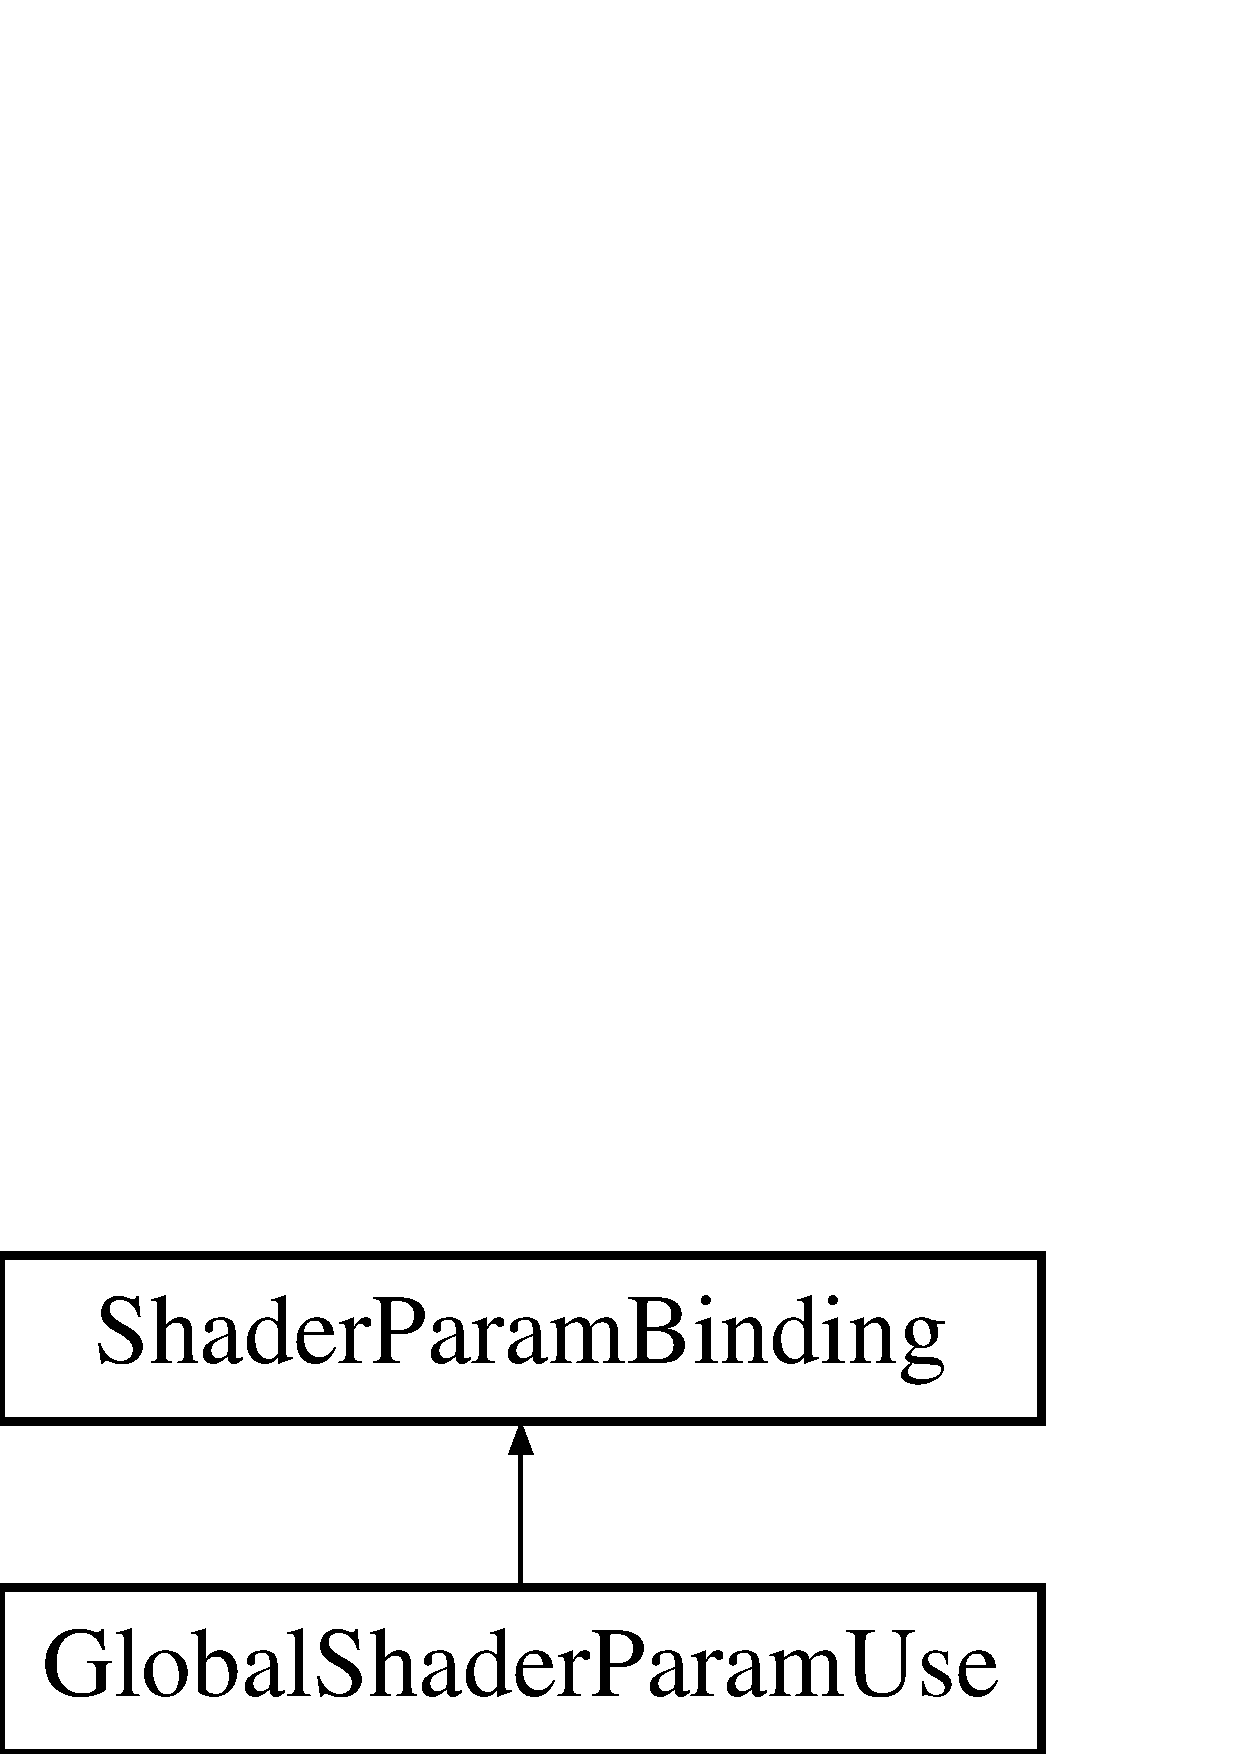
\includegraphics[height=2.000000cm]{struct_global_shader_param_use}
\end{center}
\end{figure}
\subsection*{Public Member Functions}
\begin{DoxyCompactItemize}
\item 
\mbox{\Hypertarget{struct_global_shader_param_use_a317416a619ef3bd2dd887cff7f1d582d}\label{struct_global_shader_param_use_a317416a619ef3bd2dd887cff7f1d582d}} 
void {\bfseries flush} ()
\end{DoxyCompactItemize}
\subsection*{Public Attributes}
\begin{DoxyCompactItemize}
\item 
\mbox{\Hypertarget{struct_global_shader_param_use_ac12e93cf9fcc5249bd258ab8e31bfbe0}\label{struct_global_shader_param_use_ac12e93cf9fcc5249bd258ab8e31bfbe0}} 
\hyperlink{struct_global_shader_param_state}{Global\+Shader\+Param\+State} $\ast$ {\bfseries param}
\item 
\mbox{\Hypertarget{struct_global_shader_param_use_a1a99e43aceebfeb6038cdb3dd569a77b}\label{struct_global_shader_param_use_a1a99e43aceebfeb6038cdb3dd569a77b}} 
int {\bfseries version}
\end{DoxyCompactItemize}


The documentation for this struct was generated from the following file\+:\begin{DoxyCompactItemize}
\item 
H\+:/\+Rival\+Engine/\+Rival\+\_\+\+Game\+\_\+\+Engine\+\_\+\+G\+I\+T/\+Rival3dengine/source/engine/texture.\+h\end{DoxyCompactItemize}

\hypertarget{struct_u_i_1_1_gradient}{}\section{UI\+:\+:Gradient Struct Reference}
\label{struct_u_i_1_1_gradient}\index{U\+I\+::\+Gradient@{U\+I\+::\+Gradient}}
Inheritance diagram for UI\+:\+:Gradient\+:\begin{figure}[H]
\begin{center}
\leavevmode
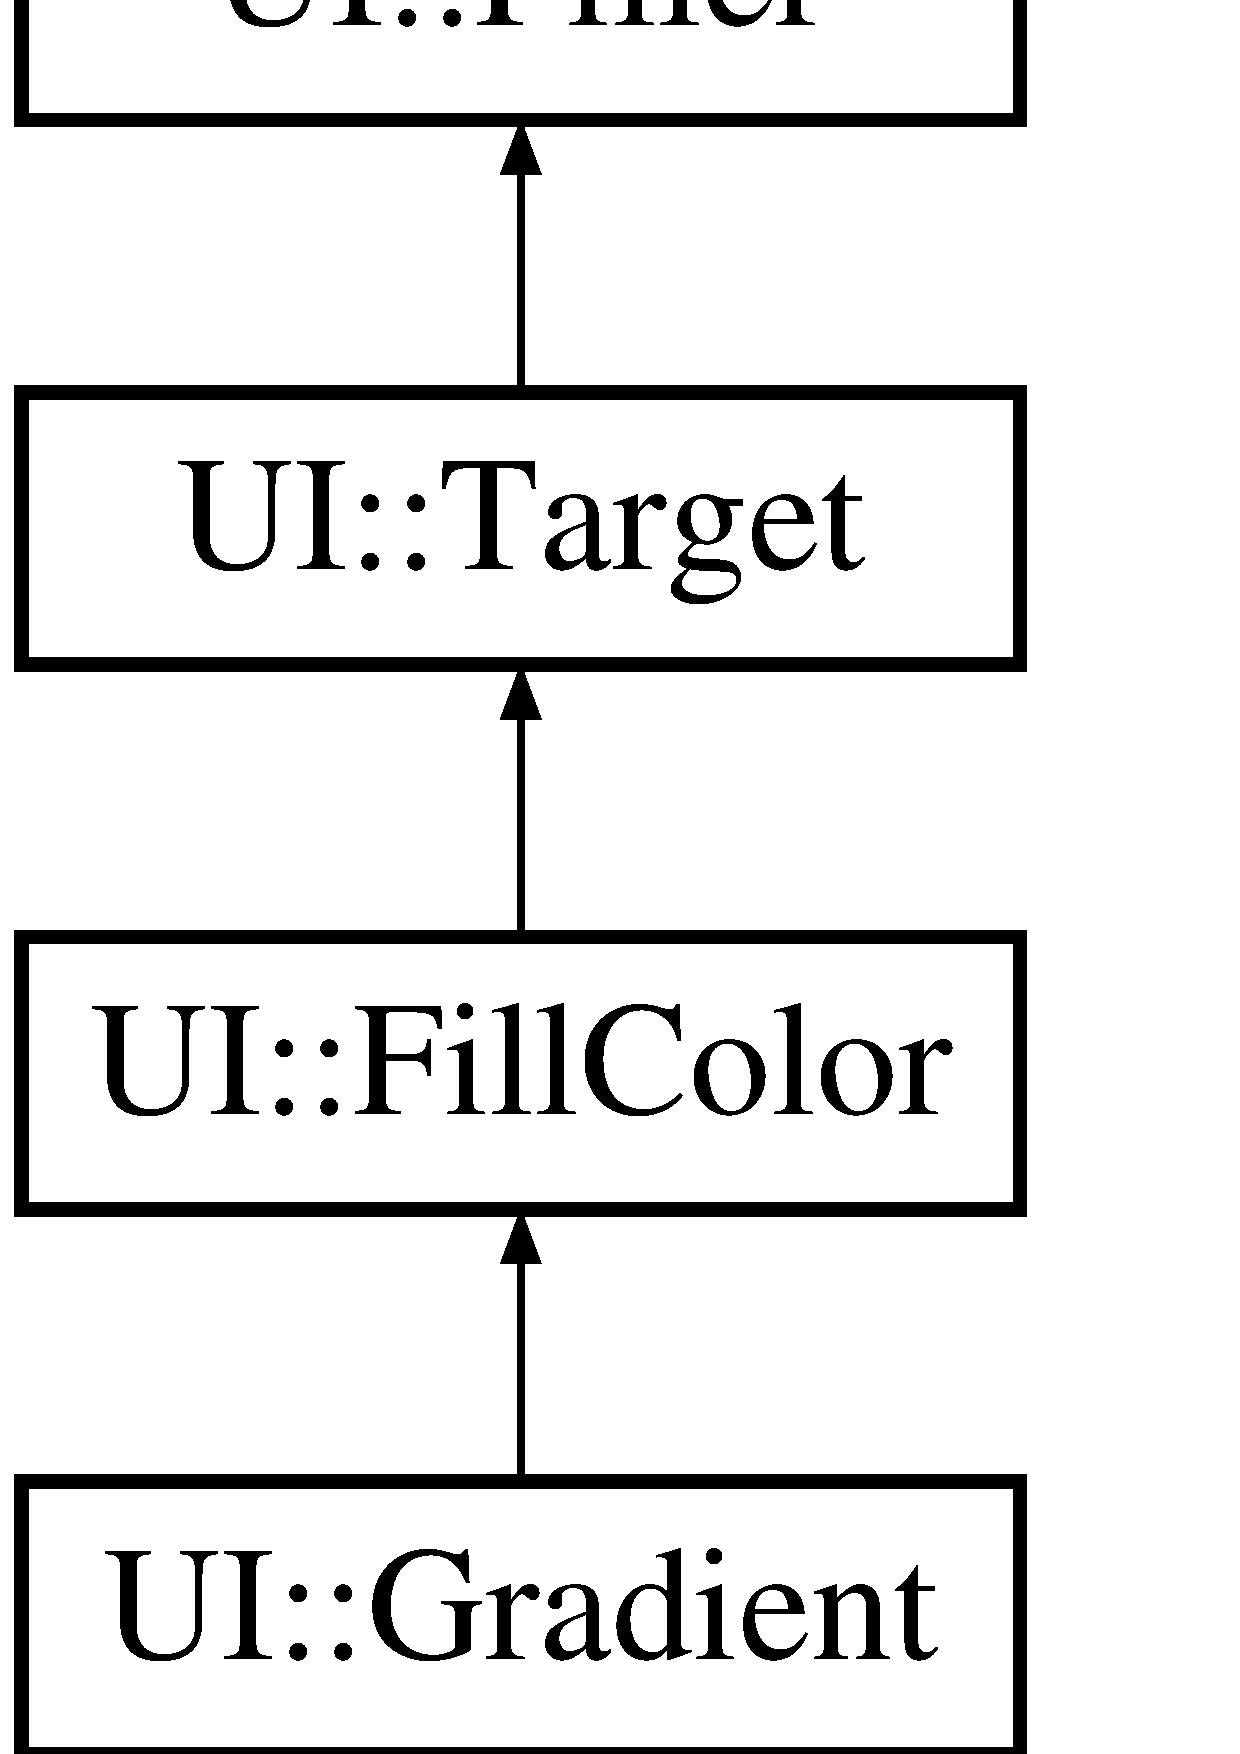
\includegraphics[height=5.000000cm]{struct_u_i_1_1_gradient}
\end{center}
\end{figure}
\subsection*{Public Types}
\begin{DoxyCompactItemize}
\item 
\mbox{\Hypertarget{struct_u_i_1_1_gradient_aca8ffac687e767aad705d3d32946e563}\label{struct_u_i_1_1_gradient_aca8ffac687e767aad705d3d32946e563}} 
enum \{ {\bfseries V\+E\+R\+T\+I\+C\+AL}, 
{\bfseries H\+O\+R\+I\+Z\+O\+N\+T\+AL}
 \}
\end{DoxyCompactItemize}
\subsection*{Public Member Functions}
\begin{DoxyCompactItemize}
\item 
\mbox{\Hypertarget{struct_u_i_1_1_gradient_a8e9b2513e77792b914edb0cce0b04461}\label{struct_u_i_1_1_gradient_a8e9b2513e77792b914edb0cce0b04461}} 
void {\bfseries setup} (int type\+\_\+, int dir\+\_\+, const \hyperlink{struct_u_i_1_1_color}{Color} \&color\+\_\+, const \hyperlink{struct_u_i_1_1_color}{Color} \&color2\+\_\+, float minw\+\_\+=0, float minh\+\_\+=0)
\item 
\mbox{\Hypertarget{struct_u_i_1_1_gradient_a87018c7d7068c0db21445238c925134d}\label{struct_u_i_1_1_gradient_a87018c7d7068c0db21445238c925134d}} 
const char $\ast$ {\bfseries gettype} () const
\item 
\mbox{\Hypertarget{struct_u_i_1_1_gradient_a109cfab811a10d065bf4220f1f177060}\label{struct_u_i_1_1_gradient_a109cfab811a10d065bf4220f1f177060}} 
void {\bfseries startdraw} ()
\item 
\mbox{\Hypertarget{struct_u_i_1_1_gradient_a868ea4a31d0d60d7abeb366b0d0f4c7a}\label{struct_u_i_1_1_gradient_a868ea4a31d0d60d7abeb366b0d0f4c7a}} 
void {\bfseries draw} (float sx, float sy)
\end{DoxyCompactItemize}
\subsection*{Static Public Member Functions}
\begin{DoxyCompactItemize}
\item 
\mbox{\Hypertarget{struct_u_i_1_1_gradient_a4ea53578f8b67fa10dc44a9646732561}\label{struct_u_i_1_1_gradient_a4ea53578f8b67fa10dc44a9646732561}} 
static const char $\ast$ {\bfseries typestr} ()
\end{DoxyCompactItemize}
\subsection*{Public Attributes}
\begin{DoxyCompactItemize}
\item 
\mbox{\Hypertarget{struct_u_i_1_1_gradient_a1ab94b6c50df223a2716ac9b76a052cf}\label{struct_u_i_1_1_gradient_a1ab94b6c50df223a2716ac9b76a052cf}} 
int {\bfseries dir}
\item 
\mbox{\Hypertarget{struct_u_i_1_1_gradient_a2be37ae45a06a0351a8c925c53a8e36f}\label{struct_u_i_1_1_gradient_a2be37ae45a06a0351a8c925c53a8e36f}} 
\hyperlink{struct_u_i_1_1_color}{Color} {\bfseries color2}
\end{DoxyCompactItemize}


The documentation for this struct was generated from the following file\+:\begin{DoxyCompactItemize}
\item 
H\+:/\+Rival\+Engine/\+Rival\+\_\+\+Game\+\_\+\+Engine\+\_\+\+G\+I\+T/\+Rival3dengine/source/engine/ui.\+cpp\end{DoxyCompactItemize}

\hypertarget{structgrassgroup}{}\section{grassgroup Struct Reference}
\label{structgrassgroup}\index{grassgroup@{grassgroup}}
\subsection*{Public Attributes}
\begin{DoxyCompactItemize}
\item 
\mbox{\Hypertarget{structgrassgroup_aec4811ba558aa691e98650203073af60}\label{structgrassgroup_aec4811ba558aa691e98650203073af60}} 
const \hyperlink{structgrasstri}{grasstri} $\ast$ {\bfseries tri}
\item 
\mbox{\Hypertarget{structgrassgroup_ab59941092fe226f388662f0e7a7e637d}\label{structgrassgroup_ab59941092fe226f388662f0e7a7e637d}} 
int {\bfseries tex}
\item 
\mbox{\Hypertarget{structgrassgroup_ac3a722e78fc93507b060f00d8eaf5fb4}\label{structgrassgroup_ac3a722e78fc93507b060f00d8eaf5fb4}} 
int {\bfseries offset}
\item 
\mbox{\Hypertarget{structgrassgroup_a46a1643c6fe891dc6756b374d2fc9b6b}\label{structgrassgroup_a46a1643c6fe891dc6756b374d2fc9b6b}} 
int {\bfseries numquads}
\end{DoxyCompactItemize}


The documentation for this struct was generated from the following file\+:\begin{DoxyCompactItemize}
\item 
H\+:/\+Rival\+Engine/\+Rival\+\_\+\+Game\+\_\+\+Engine\+\_\+\+G\+I\+T/\+Rival3dengine/source/engine/grass.\+cpp\end{DoxyCompactItemize}

\hypertarget{structgrasstri}{}\section{grasstri Struct Reference}
\label{structgrasstri}\index{grasstri@{grasstri}}
\subsection*{Public Attributes}
\begin{DoxyCompactItemize}
\item 
\mbox{\Hypertarget{structgrasstri_ae0457b175f69eec31e17b6e814e47015}\label{structgrasstri_ae0457b175f69eec31e17b6e814e47015}} 
\hyperlink{structvec}{vec} {\bfseries v} \mbox{[}4\mbox{]}
\item 
\mbox{\Hypertarget{structgrasstri_a5a968f59815df8569c44beebd36613a9}\label{structgrasstri_a5a968f59815df8569c44beebd36613a9}} 
int {\bfseries numv}
\item 
\mbox{\Hypertarget{structgrasstri_a0f756cd9807bdad475fcb67678c7b793}\label{structgrasstri_a0f756cd9807bdad475fcb67678c7b793}} 
\hyperlink{structplane}{plane} {\bfseries surface}
\item 
\mbox{\Hypertarget{structgrasstri_a1e306f2317473684afb237c746cd2097}\label{structgrasstri_a1e306f2317473684afb237c746cd2097}} 
\hyperlink{structvec}{vec} {\bfseries center}
\item 
\mbox{\Hypertarget{structgrasstri_a3518c466c9b893d6f78ad31a9bc596ea}\label{structgrasstri_a3518c466c9b893d6f78ad31a9bc596ea}} 
float {\bfseries radius}
\item 
\mbox{\Hypertarget{structgrasstri_a9e91c505776fd752705f2a46df2fa360}\label{structgrasstri_a9e91c505776fd752705f2a46df2fa360}} 
float {\bfseries minz}
\item 
\mbox{\Hypertarget{structgrasstri_a57f35c51395a9134433f8a92a41f4630}\label{structgrasstri_a57f35c51395a9134433f8a92a41f4630}} 
float {\bfseries maxz}
\item 
\mbox{\Hypertarget{structgrasstri_a1b0fef5fd27c75bada97a346564afbb6}\label{structgrasstri_a1b0fef5fd27c75bada97a346564afbb6}} 
ushort {\bfseries texture}
\item 
\mbox{\Hypertarget{structgrasstri_a5655eb1cc853126dcae8054d514fd0bd}\label{structgrasstri_a5655eb1cc853126dcae8054d514fd0bd}} 
ushort {\bfseries blend}
\end{DoxyCompactItemize}


The documentation for this struct was generated from the following file\+:\begin{DoxyCompactItemize}
\item 
H\+:/\+Rival\+Engine/\+Rival\+\_\+\+Game\+\_\+\+Engine\+\_\+\+G\+I\+T/\+Rival3dengine/source/engine/octa.\+h\end{DoxyCompactItemize}

\hypertarget{structgrassvert}{}\section{grassvert Struct Reference}
\label{structgrassvert}\index{grassvert@{grassvert}}
\subsection*{Public Attributes}
\begin{DoxyCompactItemize}
\item 
\mbox{\Hypertarget{structgrassvert_a17aa75c6105d5ccfdbb795bb24f43075}\label{structgrassvert_a17aa75c6105d5ccfdbb795bb24f43075}} 
\hyperlink{structvec}{vec} {\bfseries pos}
\item 
\mbox{\Hypertarget{structgrassvert_ad16d70c6d060718dae6aeabfde03aa34}\label{structgrassvert_ad16d70c6d060718dae6aeabfde03aa34}} 
\hyperlink{structbvec4}{bvec4} {\bfseries color}
\item 
\mbox{\Hypertarget{structgrassvert_abad5a052083196ca8db8ce534e69589f}\label{structgrassvert_abad5a052083196ca8db8ce534e69589f}} 
float {\bfseries u}
\item 
\mbox{\Hypertarget{structgrassvert_a4bf966fe084bbe255000bb71efd220ec}\label{structgrassvert_a4bf966fe084bbe255000bb71efd220ec}} 
float {\bfseries v}
\end{DoxyCompactItemize}


The documentation for this struct was generated from the following file\+:\begin{DoxyCompactItemize}
\item 
H\+:/\+Rival\+Engine/\+Rival\+\_\+\+Game\+\_\+\+Engine\+\_\+\+G\+I\+T/\+Rival3dengine/source/engine/grass.\+cpp\end{DoxyCompactItemize}

\hypertarget{struct_u_i_1_1_grid}{}\section{UI\+:\+:Grid Struct Reference}
\label{struct_u_i_1_1_grid}\index{U\+I\+::\+Grid@{U\+I\+::\+Grid}}
Inheritance diagram for UI\+:\+:Grid\+:\begin{figure}[H]
\begin{center}
\leavevmode
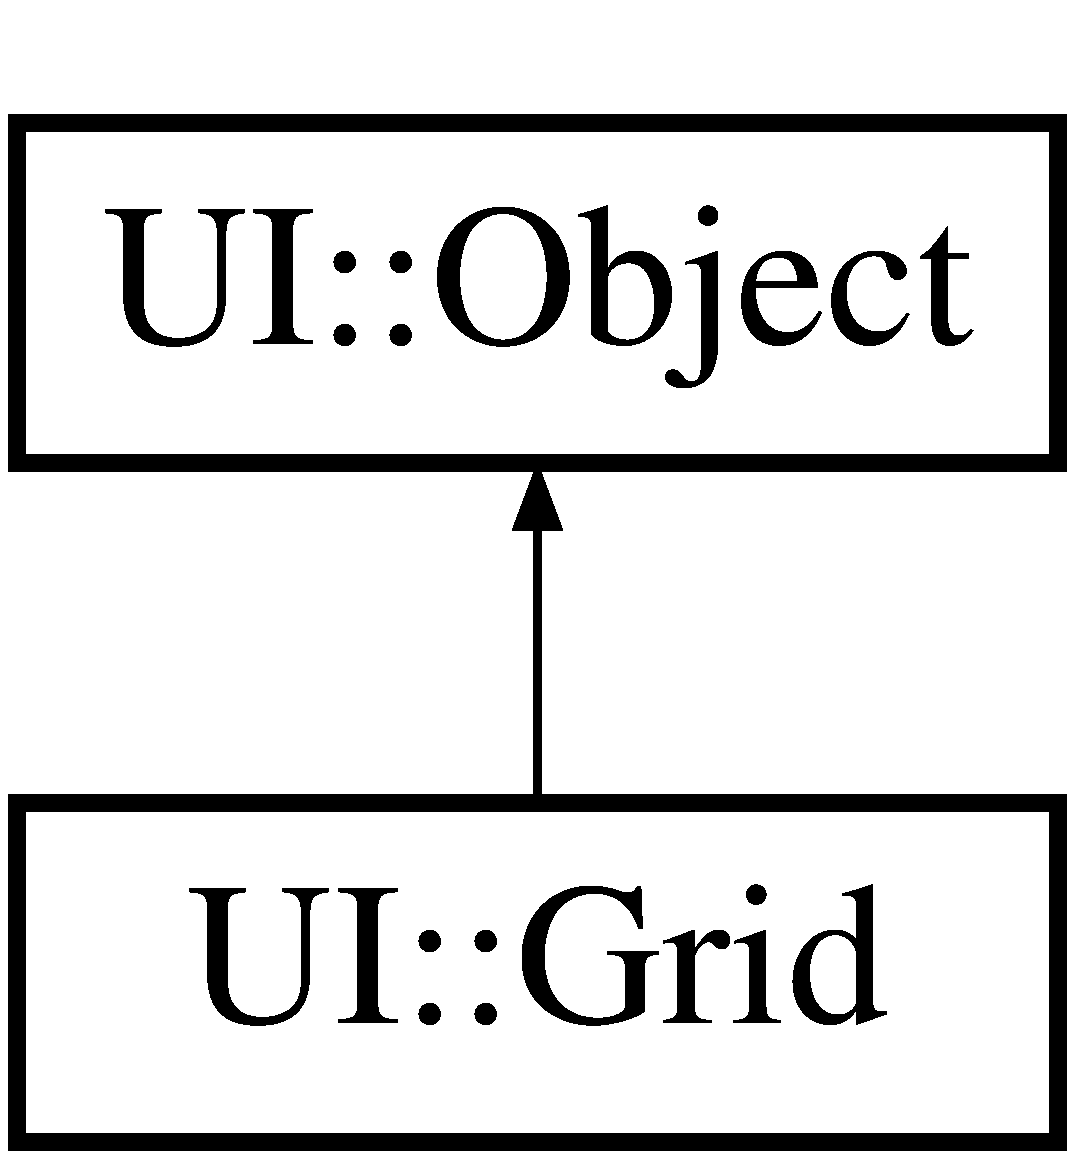
\includegraphics[height=2.000000cm]{struct_u_i_1_1_grid}
\end{center}
\end{figure}
\subsection*{Public Member Functions}
\begin{DoxyCompactItemize}
\item 
\mbox{\Hypertarget{struct_u_i_1_1_grid_a8a236da5bb2b9dc64c238536741d227d}\label{struct_u_i_1_1_grid_a8a236da5bb2b9dc64c238536741d227d}} 
const char $\ast$ {\bfseries gettype} () const
\item 
\mbox{\Hypertarget{struct_u_i_1_1_grid_a58dc4fe7915ddade60578bceab0b261a}\label{struct_u_i_1_1_grid_a58dc4fe7915ddade60578bceab0b261a}} 
void {\bfseries setup} (int columns\+\_\+, float spacew\+\_\+=0, float spaceh\+\_\+=0)
\item 
\mbox{\Hypertarget{struct_u_i_1_1_grid_ab088f45a40e2a44e151a58d82a2e3af3}\label{struct_u_i_1_1_grid_ab088f45a40e2a44e151a58d82a2e3af3}} 
uchar {\bfseries childalign} () const
\item 
\mbox{\Hypertarget{struct_u_i_1_1_grid_added9e84e7f83d1286f99f8c7964519a}\label{struct_u_i_1_1_grid_added9e84e7f83d1286f99f8c7964519a}} 
void {\bfseries layout} ()
\item 
\mbox{\Hypertarget{struct_u_i_1_1_grid_a52b4e41e3d971aadec08b249b71a14d1}\label{struct_u_i_1_1_grid_a52b4e41e3d971aadec08b249b71a14d1}} 
void {\bfseries adjustchildren} ()
\end{DoxyCompactItemize}
\subsection*{Static Public Member Functions}
\begin{DoxyCompactItemize}
\item 
\mbox{\Hypertarget{struct_u_i_1_1_grid_aa1367cc179a538b296e3d4e1166f2644}\label{struct_u_i_1_1_grid_aa1367cc179a538b296e3d4e1166f2644}} 
static const char $\ast$ {\bfseries typestr} ()
\end{DoxyCompactItemize}
\subsection*{Public Attributes}
\begin{DoxyCompactItemize}
\item 
\mbox{\Hypertarget{struct_u_i_1_1_grid_a6d54ef76d1b8149de22bdc21ae5247a5}\label{struct_u_i_1_1_grid_a6d54ef76d1b8149de22bdc21ae5247a5}} 
int {\bfseries columns}
\item 
\mbox{\Hypertarget{struct_u_i_1_1_grid_a05c2aba53a171263a596a3590597f0f3}\label{struct_u_i_1_1_grid_a05c2aba53a171263a596a3590597f0f3}} 
float {\bfseries spacew}
\item 
\mbox{\Hypertarget{struct_u_i_1_1_grid_a55dc1d2769ea4c5e9cfe5e4d3e54fc29}\label{struct_u_i_1_1_grid_a55dc1d2769ea4c5e9cfe5e4d3e54fc29}} 
float {\bfseries spaceh}
\item 
\mbox{\Hypertarget{struct_u_i_1_1_grid_a8e171bc821d6f6ced9a1fd77cf1140e0}\label{struct_u_i_1_1_grid_a8e171bc821d6f6ced9a1fd77cf1140e0}} 
float {\bfseries subw}
\item 
\mbox{\Hypertarget{struct_u_i_1_1_grid_aff66d17be070d390c8e806d8bd3b3081}\label{struct_u_i_1_1_grid_aff66d17be070d390c8e806d8bd3b3081}} 
float {\bfseries subh}
\item 
\mbox{\Hypertarget{struct_u_i_1_1_grid_a70db1c7be6a74d3f6040aaa3e8954be8}\label{struct_u_i_1_1_grid_a70db1c7be6a74d3f6040aaa3e8954be8}} 
\hyperlink{structvector}{vector}$<$ float $>$ {\bfseries widths}
\item 
\mbox{\Hypertarget{struct_u_i_1_1_grid_a9b3be6f075167bcc208890c3d07dd848}\label{struct_u_i_1_1_grid_a9b3be6f075167bcc208890c3d07dd848}} 
\hyperlink{structvector}{vector}$<$ float $>$ {\bfseries heights}
\end{DoxyCompactItemize}


The documentation for this struct was generated from the following file\+:\begin{DoxyCompactItemize}
\item 
H\+:/\+Rival\+Engine/\+Rival\+\_\+\+Game\+\_\+\+Engine\+\_\+\+G\+I\+T/\+Rival3dengine/source/engine/ui.\+cpp\end{DoxyCompactItemize}

\hypertarget{structgzstream}{}\section{gzstream Struct Reference}
\label{structgzstream}\index{gzstream@{gzstream}}
Inheritance diagram for gzstream\+:\begin{figure}[H]
\begin{center}
\leavevmode
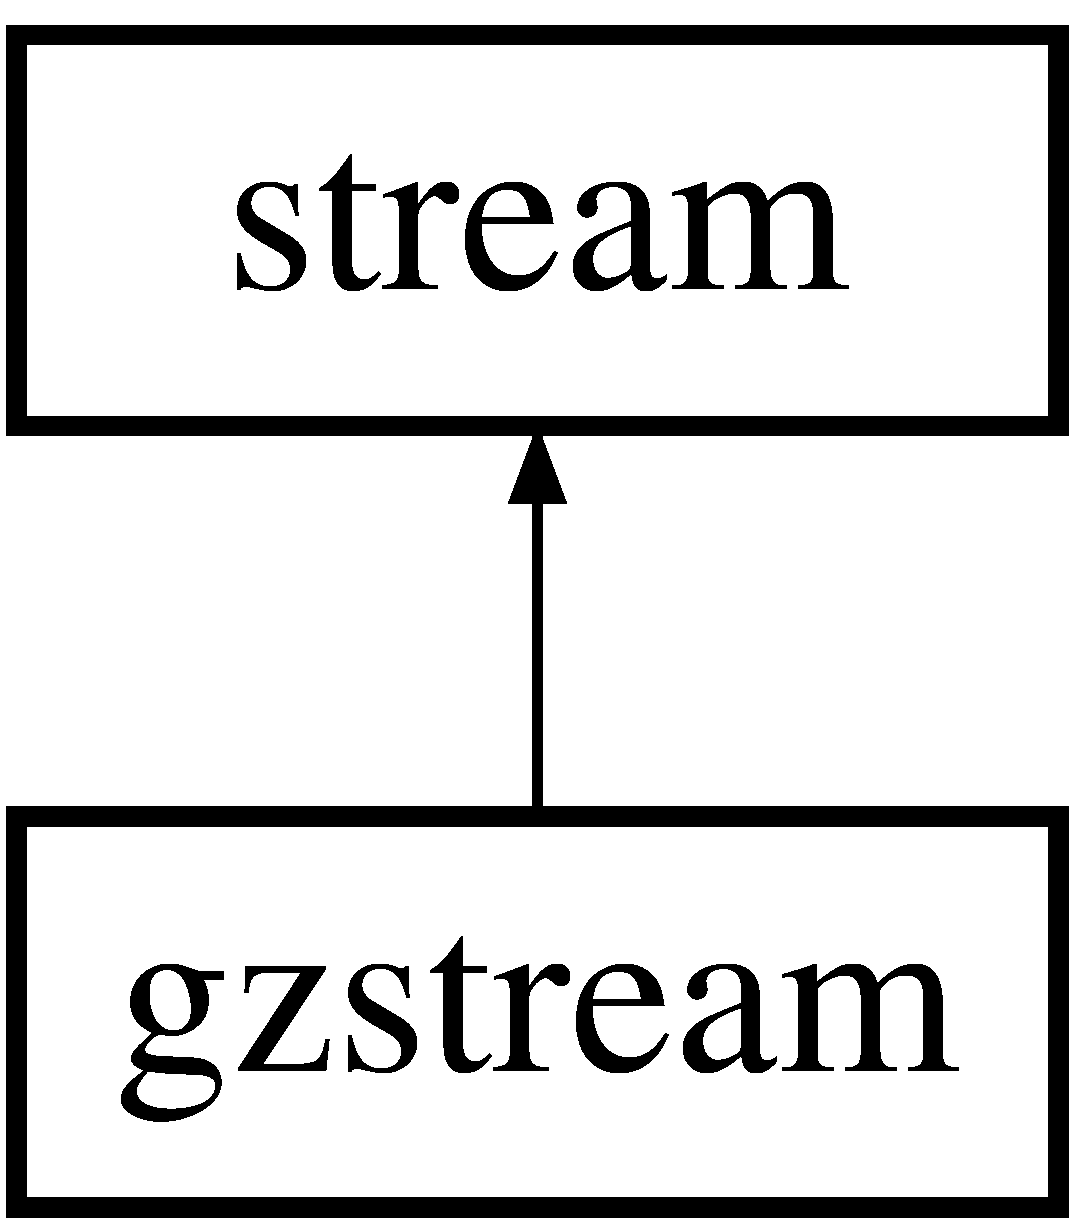
\includegraphics[height=2.000000cm]{structgzstream}
\end{center}
\end{figure}
\subsection*{Public Types}
\begin{DoxyCompactItemize}
\item 
\mbox{\Hypertarget{structgzstream_a140871c2fa96253cb29b76bb58b9c76a}\label{structgzstream_a140871c2fa96253cb29b76bb58b9c76a}} 
enum \{ {\bfseries M\+A\+G\+I\+C1} = 0x1F, 
{\bfseries M\+A\+G\+I\+C2} = 0x8B, 
{\bfseries B\+U\+F\+S\+I\+ZE} = 16384, 
{\bfseries O\+S\+\_\+\+U\+N\+IX} = 0x03
 \}
\item 
\mbox{\Hypertarget{structgzstream_ac34b61c709a5fb76430cb31b00266a55}\label{structgzstream_ac34b61c709a5fb76430cb31b00266a55}} 
enum \{ \newline
{\bfseries F\+\_\+\+A\+S\+C\+II} = 0x01, 
{\bfseries F\+\_\+\+C\+RC} = 0x02, 
{\bfseries F\+\_\+\+E\+X\+T\+RA} = 0x04, 
{\bfseries F\+\_\+\+N\+A\+ME} = 0x08, 
\newline
{\bfseries F\+\_\+\+C\+O\+M\+M\+E\+NT} = 0x10, 
{\bfseries F\+\_\+\+R\+E\+S\+E\+R\+V\+ED} = 0x\+E0
 \}
\end{DoxyCompactItemize}
\subsection*{Public Member Functions}
\begin{DoxyCompactItemize}
\item 
\mbox{\Hypertarget{structgzstream_a6d191853a1c4c8bf6cccbab9c8e0309a}\label{structgzstream_a6d191853a1c4c8bf6cccbab9c8e0309a}} 
void {\bfseries writeheader} ()
\item 
\mbox{\Hypertarget{structgzstream_a8d0344b10ddf5d5f027f845b25a5d7b7}\label{structgzstream_a8d0344b10ddf5d5f027f845b25a5d7b7}} 
void {\bfseries readbuf} (size\+\_\+t size=B\+U\+F\+S\+I\+ZE)
\item 
\mbox{\Hypertarget{structgzstream_a4da22015c7effe15411cec2f24dea196}\label{structgzstream_a4da22015c7effe15411cec2f24dea196}} 
uchar {\bfseries readbyte} (size\+\_\+t size=B\+U\+F\+S\+I\+ZE)
\item 
\mbox{\Hypertarget{structgzstream_a03650110ed9c2b4d0b055347fa2597c9}\label{structgzstream_a03650110ed9c2b4d0b055347fa2597c9}} 
void {\bfseries skipbytes} (size\+\_\+t n)
\item 
\mbox{\Hypertarget{structgzstream_a68b93da33e4709a1fd002542a78fc944}\label{structgzstream_a68b93da33e4709a1fd002542a78fc944}} 
bool {\bfseries checkheader} ()
\item 
\mbox{\Hypertarget{structgzstream_a68ed86a7e5317f5e78ab711792a03d2c}\label{structgzstream_a68ed86a7e5317f5e78ab711792a03d2c}} 
bool {\bfseries open} (\hyperlink{structstream}{stream} $\ast$f, const char $\ast$mode, bool needclose, int level)
\item 
\mbox{\Hypertarget{structgzstream_a1dbc14c5f33576998da060e4deb20d61}\label{structgzstream_a1dbc14c5f33576998da060e4deb20d61}} 
uint {\bfseries getcrc} ()
\item 
\mbox{\Hypertarget{structgzstream_a256c3b94fc42c95c6ee3cc4723e5cb8f}\label{structgzstream_a256c3b94fc42c95c6ee3cc4723e5cb8f}} 
void {\bfseries finishreading} ()
\item 
\mbox{\Hypertarget{structgzstream_a1c6cf7dae9e68e6572b506527d02bac3}\label{structgzstream_a1c6cf7dae9e68e6572b506527d02bac3}} 
void {\bfseries stopreading} ()
\item 
\mbox{\Hypertarget{structgzstream_a38f6ae18fdaa4745809c96fba06e0b33}\label{structgzstream_a38f6ae18fdaa4745809c96fba06e0b33}} 
void {\bfseries finishwriting} ()
\item 
\mbox{\Hypertarget{structgzstream_a51c351b6b6cb48ca2f0df3e116380d92}\label{structgzstream_a51c351b6b6cb48ca2f0df3e116380d92}} 
void {\bfseries stopwriting} ()
\item 
\mbox{\Hypertarget{structgzstream_a6b7351f0159775427d057bf943616586}\label{structgzstream_a6b7351f0159775427d057bf943616586}} 
void {\bfseries close} ()
\item 
\mbox{\Hypertarget{structgzstream_a48d86482e0ce4b9c9366a142bf508bf9}\label{structgzstream_a48d86482e0ce4b9c9366a142bf508bf9}} 
bool {\bfseries end} ()
\item 
\mbox{\Hypertarget{structgzstream_a223b6be23775308a71a0b89306ca6699}\label{structgzstream_a223b6be23775308a71a0b89306ca6699}} 
offset {\bfseries tell} ()
\item 
\mbox{\Hypertarget{structgzstream_a6dbe81bda0ed7df67d3f2a7de2f220ec}\label{structgzstream_a6dbe81bda0ed7df67d3f2a7de2f220ec}} 
offset {\bfseries rawtell} ()
\item 
\mbox{\Hypertarget{structgzstream_a4ce93622b9e6f397253e3918f7f6576f}\label{structgzstream_a4ce93622b9e6f397253e3918f7f6576f}} 
offset {\bfseries size} ()
\item 
\mbox{\Hypertarget{structgzstream_accf7a7e788746b542fe5a8d4d4f29156}\label{structgzstream_accf7a7e788746b542fe5a8d4d4f29156}} 
offset {\bfseries rawsize} ()
\item 
\mbox{\Hypertarget{structgzstream_a40cd78f7ee55c7a699f558a97dc8b757}\label{structgzstream_a40cd78f7ee55c7a699f558a97dc8b757}} 
bool {\bfseries seek} (offset pos, int whence)
\item 
\mbox{\Hypertarget{structgzstream_a4181c3543a5af7649e7e07fd7e9c69fe}\label{structgzstream_a4181c3543a5af7649e7e07fd7e9c69fe}} 
size\+\_\+t {\bfseries read} (void $\ast$buf, size\+\_\+t len)
\item 
\mbox{\Hypertarget{structgzstream_aac92c3ac4dbee68231652e59a678daae}\label{structgzstream_aac92c3ac4dbee68231652e59a678daae}} 
bool {\bfseries flushbuf} (bool full=false)
\item 
\mbox{\Hypertarget{structgzstream_a72f08de4d18360defb6341b814f38374}\label{structgzstream_a72f08de4d18360defb6341b814f38374}} 
bool {\bfseries flush} ()
\item 
\mbox{\Hypertarget{structgzstream_a68167b020a7931ad0e840dc46f0b70bb}\label{structgzstream_a68167b020a7931ad0e840dc46f0b70bb}} 
size\+\_\+t {\bfseries write} (const void $\ast$buf, size\+\_\+t len)
\end{DoxyCompactItemize}
\subsection*{Public Attributes}
\begin{DoxyCompactItemize}
\item 
\mbox{\Hypertarget{structgzstream_a89047b896f1447130986efd6ba911bfc}\label{structgzstream_a89047b896f1447130986efd6ba911bfc}} 
\hyperlink{structstream}{stream} $\ast$ {\bfseries file}
\item 
\mbox{\Hypertarget{structgzstream_aa0729b97e2ad985fb251b03a97a631b1}\label{structgzstream_aa0729b97e2ad985fb251b03a97a631b1}} 
z\+\_\+stream {\bfseries zfile}
\item 
\mbox{\Hypertarget{structgzstream_a3fa23c603a2059d72fad3ad5624091ae}\label{structgzstream_a3fa23c603a2059d72fad3ad5624091ae}} 
uchar $\ast$ {\bfseries buf}
\item 
\mbox{\Hypertarget{structgzstream_ab7b3fb548a1d64d7ee97239ce450c836}\label{structgzstream_ab7b3fb548a1d64d7ee97239ce450c836}} 
bool {\bfseries reading}
\item 
\mbox{\Hypertarget{structgzstream_a22e23d033e552da74b50baf01a93ddf3}\label{structgzstream_a22e23d033e552da74b50baf01a93ddf3}} 
bool {\bfseries writing}
\item 
\mbox{\Hypertarget{structgzstream_aadb50ea1af1910707fec74525d19dc6e}\label{structgzstream_aadb50ea1af1910707fec74525d19dc6e}} 
bool {\bfseries autoclose}
\item 
\mbox{\Hypertarget{structgzstream_af29aa1e4c730531a7d75a5b755cbeaf1}\label{structgzstream_af29aa1e4c730531a7d75a5b755cbeaf1}} 
uint {\bfseries crc}
\item 
\mbox{\Hypertarget{structgzstream_adfe5d25c1649bd8da86f4e8a7e2fe9b3}\label{structgzstream_adfe5d25c1649bd8da86f4e8a7e2fe9b3}} 
size\+\_\+t {\bfseries headersize}
\end{DoxyCompactItemize}


The documentation for this struct was generated from the following file\+:\begin{DoxyCompactItemize}
\item 
H\+:/\+Rival\+Engine/\+Rival\+\_\+\+Game\+\_\+\+Engine\+\_\+\+G\+I\+T/\+Rival3dengine/source/shared/stream.\+cpp\end{DoxyCompactItemize}

\hypertarget{structhalf}{}\section{half Struct Reference}
\label{structhalf}\index{half@{half}}
\subsection*{Public Member Functions}
\begin{DoxyCompactItemize}
\item 
\mbox{\Hypertarget{structhalf_a99acfa5329e169f52964715cecda3233}\label{structhalf_a99acfa5329e169f52964715cecda3233}} 
{\bfseries half} (float f)
\item 
\mbox{\Hypertarget{structhalf_abe001f5a30c1ac90109858cb3e743f5f}\label{structhalf_abe001f5a30c1ac90109858cb3e743f5f}} 
bool {\bfseries operator==} (const \hyperlink{structhalf}{half} \&h) const
\item 
\mbox{\Hypertarget{structhalf_ad9c135c856dd827c8b3df0c81a0f3ec3}\label{structhalf_ad9c135c856dd827c8b3df0c81a0f3ec3}} 
bool {\bfseries operator!=} (const \hyperlink{structhalf}{half} \&h) const
\end{DoxyCompactItemize}
\subsection*{Public Attributes}
\begin{DoxyCompactItemize}
\item 
\mbox{\Hypertarget{structhalf_ae0c58bfb0408fe23acd894d1b936f3d9}\label{structhalf_ae0c58bfb0408fe23acd894d1b936f3d9}} 
ushort {\bfseries val}
\end{DoxyCompactItemize}


The documentation for this struct was generated from the following file\+:\begin{DoxyCompactItemize}
\item 
H\+:/\+Rival\+Engine/\+Rival\+\_\+\+Game\+\_\+\+Engine\+\_\+\+G\+I\+T/\+Rival3dengine/source/shared/geom.\+h\end{DoxyCompactItemize}

\hypertarget{structhashbase}{}\section{hashbase$<$ H, E, K, T $>$ Struct Template Reference}
\label{structhashbase}\index{hashbase$<$ H, E, K, T $>$@{hashbase$<$ H, E, K, T $>$}}
\subsection*{Classes}
\begin{DoxyCompactItemize}
\item 
struct \hyperlink{structhashbase_1_1chain}{chain}
\item 
struct \hyperlink{structhashbase_1_1chainchunk}{chainchunk}
\end{DoxyCompactItemize}
\subsection*{Public Types}
\begin{DoxyCompactItemize}
\item 
\mbox{\Hypertarget{structhashbase_a23d764580f45007f5e835976cb86e07c}\label{structhashbase_a23d764580f45007f5e835976cb86e07c}} 
enum \{ {\bfseries C\+H\+U\+N\+K\+S\+I\+ZE} = 64
 \}
\item 
\mbox{\Hypertarget{structhashbase_af9b3b2fac33b501ffe9bc31f3ee53a4c}\label{structhashbase_af9b3b2fac33b501ffe9bc31f3ee53a4c}} 
enum \{ {\bfseries D\+E\+F\+A\+U\+L\+T\+S\+I\+ZE} = 1$<$$<$10
 \}
\item 
\mbox{\Hypertarget{structhashbase_a6cb82d402e0c7d9bd770722d8d1eb6df}\label{structhashbase_a6cb82d402e0c7d9bd770722d8d1eb6df}} 
typedef E {\bfseries elemtype}
\item 
\mbox{\Hypertarget{structhashbase_a1d6055f94835a81eae6fd7f70d180f1e}\label{structhashbase_a1d6055f94835a81eae6fd7f70d180f1e}} 
typedef K {\bfseries keytype}
\item 
\mbox{\Hypertarget{structhashbase_ae97da04ae671d9246ddd1326f3931f78}\label{structhashbase_ae97da04ae671d9246ddd1326f3931f78}} 
typedef T {\bfseries datatype}
\end{DoxyCompactItemize}
\subsection*{Public Member Functions}
\begin{DoxyCompactItemize}
\item 
\mbox{\Hypertarget{structhashbase_af21a8ef4ce7ae76ebab5971533521a59}\label{structhashbase_af21a8ef4ce7ae76ebab5971533521a59}} 
{\bfseries hashbase} (int size=D\+E\+F\+A\+U\+L\+T\+S\+I\+ZE)
\item 
\mbox{\Hypertarget{structhashbase_ad04058aa2b5a25cb6c61236d3d2b542f}\label{structhashbase_ad04058aa2b5a25cb6c61236d3d2b542f}} 
\hyperlink{structhashbase_1_1chain}{chain} $\ast$ {\bfseries insert} (uint h)
\item 
\mbox{\Hypertarget{structhashbase_abd035efc8a331bfb0856bfe1ba6e9a55}\label{structhashbase_abd035efc8a331bfb0856bfe1ba6e9a55}} 
{\footnotesize template$<$class U $>$ }\\T \& {\bfseries insert} (uint h, const U \&key)
\item 
\mbox{\Hypertarget{structhashbase_a12163e20ba78e48400771dbd6b8cbe5b}\label{structhashbase_a12163e20ba78e48400771dbd6b8cbe5b}} 
{\footnotesize template$<$class U $>$ }\\T $\ast$ {\bfseries access} (const U \&key)
\item 
\mbox{\Hypertarget{structhashbase_ab52626a876edc969af522e2c94658dbd}\label{structhashbase_ab52626a876edc969af522e2c94658dbd}} 
{\footnotesize template$<$class U , class V $>$ }\\T \& {\bfseries access} (const U \&key, const V \&elem)
\item 
\mbox{\Hypertarget{structhashbase_a6c546956b0685adbde081c0fe1bb5c42}\label{structhashbase_a6c546956b0685adbde081c0fe1bb5c42}} 
{\footnotesize template$<$class V $>$ }\\T \& {\bfseries add} (const V \&elem)
\item 
\mbox{\Hypertarget{structhashbase_a55e85b351ca5cf32978f5c08ef413f9b}\label{structhashbase_a55e85b351ca5cf32978f5c08ef413f9b}} 
{\footnotesize template$<$class U $>$ }\\T \& {\bfseries operator\mbox{[}$\,$\mbox{]}} (const U \&key)
\item 
\mbox{\Hypertarget{structhashbase_ae0be9b1b7ef3e6fa27b2fdfff0482d80}\label{structhashbase_ae0be9b1b7ef3e6fa27b2fdfff0482d80}} 
{\footnotesize template$<$class U $>$ }\\T \& {\bfseries find} (const U \&key, T \&notfound)
\item 
\mbox{\Hypertarget{structhashbase_a151c6709ccf7b057e9f0e841fd67fda9}\label{structhashbase_a151c6709ccf7b057e9f0e841fd67fda9}} 
{\footnotesize template$<$class U $>$ }\\const T \& {\bfseries find} (const U \&key, const T \&notfound)
\item 
\mbox{\Hypertarget{structhashbase_ae032e2e2ea6f7caddb77d03501fcb9cd}\label{structhashbase_ae032e2e2ea6f7caddb77d03501fcb9cd}} 
{\footnotesize template$<$class U $>$ }\\bool {\bfseries remove} (const U \&key)
\item 
\mbox{\Hypertarget{structhashbase_a1a50ac106c87f05a155037698d8887fe}\label{structhashbase_a1a50ac106c87f05a155037698d8887fe}} 
void {\bfseries recycle} ()
\item 
\mbox{\Hypertarget{structhashbase_a1ef02c93cfa6e0d59c14d4a09d99db2d}\label{structhashbase_a1ef02c93cfa6e0d59c14d4a09d99db2d}} 
void {\bfseries deletechunks} ()
\item 
\mbox{\Hypertarget{structhashbase_aaee9d8fca8fb4077defa31be500b643d}\label{structhashbase_aaee9d8fca8fb4077defa31be500b643d}} 
void {\bfseries clear} ()
\end{DoxyCompactItemize}
\subsection*{Static Public Member Functions}
\begin{DoxyCompactItemize}
\item 
\mbox{\Hypertarget{structhashbase_aad23144a39ee5bb6cf549a86664e26a7}\label{structhashbase_aad23144a39ee5bb6cf549a86664e26a7}} 
static \hyperlink{structhashbase_1_1chain}{chain} $\ast$ {\bfseries enumnext} (void $\ast$i)
\item 
\mbox{\Hypertarget{structhashbase_a0ef25f4bde4909fa55b32ca430b1e5e6}\label{structhashbase_a0ef25f4bde4909fa55b32ca430b1e5e6}} 
static K \& {\bfseries enumkey} (void $\ast$i)
\item 
\mbox{\Hypertarget{structhashbase_ad25120ee6c3050418948bda379115560}\label{structhashbase_ad25120ee6c3050418948bda379115560}} 
static T \& {\bfseries enumdata} (void $\ast$i)
\end{DoxyCompactItemize}
\subsection*{Public Attributes}
\begin{DoxyCompactItemize}
\item 
\mbox{\Hypertarget{structhashbase_a600b191339f6da94d03bd9d69bcd9baf}\label{structhashbase_a600b191339f6da94d03bd9d69bcd9baf}} 
int {\bfseries size}
\item 
\mbox{\Hypertarget{structhashbase_a330deb84e27f14c22f27d870f3686c56}\label{structhashbase_a330deb84e27f14c22f27d870f3686c56}} 
int {\bfseries numelems}
\item 
\mbox{\Hypertarget{structhashbase_a94b490f872197369d1cdf618a5bcaf95}\label{structhashbase_a94b490f872197369d1cdf618a5bcaf95}} 
\hyperlink{structhashbase_1_1chain}{chain} $\ast$$\ast$ {\bfseries chains}
\item 
\mbox{\Hypertarget{structhashbase_a558356b897ae6305cdf9365fcdd76d1b}\label{structhashbase_a558356b897ae6305cdf9365fcdd76d1b}} 
\hyperlink{structhashbase_1_1chainchunk}{chainchunk} $\ast$ {\bfseries chunks}
\item 
\mbox{\Hypertarget{structhashbase_a2e6fb865c933c90e21b4b0ec504d7a63}\label{structhashbase_a2e6fb865c933c90e21b4b0ec504d7a63}} 
\hyperlink{structhashbase_1_1chain}{chain} $\ast$ {\bfseries unused}
\end{DoxyCompactItemize}


The documentation for this struct was generated from the following file\+:\begin{DoxyCompactItemize}
\item 
H\+:/\+Rival\+Engine/\+Rival\+\_\+\+Game\+\_\+\+Engine\+\_\+\+G\+I\+T/\+Rival3dengine/source/shared/tools.\+h\end{DoxyCompactItemize}

\hypertarget{structhashnameset}{}\section{hashnameset$<$ T $>$ Struct Template Reference}
\label{structhashnameset}\index{hashnameset$<$ T $>$@{hashnameset$<$ T $>$}}
Inheritance diagram for hashnameset$<$ T $>$\+:\begin{figure}[H]
\begin{center}
\leavevmode
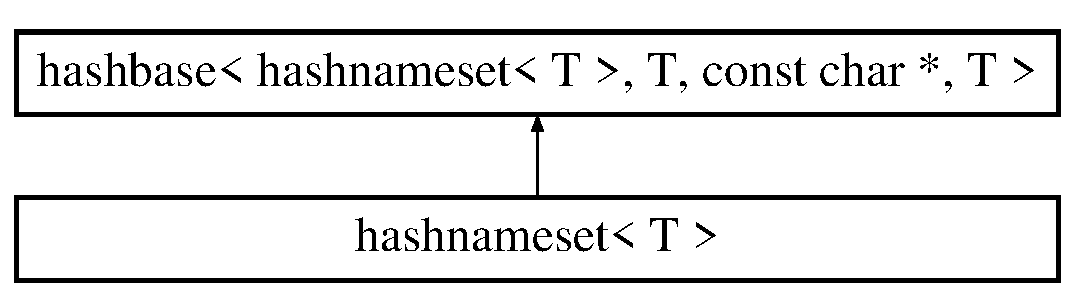
\includegraphics[height=2.000000cm]{structhashnameset}
\end{center}
\end{figure}
\subsection*{Public Types}
\begin{DoxyCompactItemize}
\item 
\mbox{\Hypertarget{structhashnameset_a637b59be44148940a0bd00183c43b8f8}\label{structhashnameset_a637b59be44148940a0bd00183c43b8f8}} 
typedef \hyperlink{structhashbase}{hashbase}$<$ \hyperlink{structhashnameset}{hashnameset}$<$ T $>$, T, const char $\ast$, T $>$ {\bfseries basetype}
\end{DoxyCompactItemize}
\subsection*{Public Member Functions}
\begin{DoxyCompactItemize}
\item 
\mbox{\Hypertarget{structhashnameset_a3a84c272e4e7e1052ae7ddfc2fc1a16e}\label{structhashnameset_a3a84c272e4e7e1052ae7ddfc2fc1a16e}} 
{\bfseries hashnameset} (int size=basetype\+::\+D\+E\+F\+A\+U\+L\+T\+S\+I\+ZE)
\end{DoxyCompactItemize}
\subsection*{Static Public Member Functions}
\begin{DoxyCompactItemize}
\item 
\mbox{\Hypertarget{structhashnameset_a33a5a5de61bdd0f6a3c51901f1f35cf1}\label{structhashnameset_a33a5a5de61bdd0f6a3c51901f1f35cf1}} 
{\footnotesize template$<$class U $>$ }\\static const char $\ast$ {\bfseries getkey} (const U \&elem)
\item 
\mbox{\Hypertarget{structhashnameset_a2c53f3c121f1ba50e87e18edebb49a53}\label{structhashnameset_a2c53f3c121f1ba50e87e18edebb49a53}} 
{\footnotesize template$<$class U $>$ }\\static const char $\ast$ {\bfseries getkey} (U $\ast$elem)
\item 
\mbox{\Hypertarget{structhashnameset_a4e24ee4456265787e539368b10db459e}\label{structhashnameset_a4e24ee4456265787e539368b10db459e}} 
static T \& {\bfseries getdata} (T \&elem)
\item 
\mbox{\Hypertarget{structhashnameset_a959f269b8e5508d152241b9650435a7f}\label{structhashnameset_a959f269b8e5508d152241b9650435a7f}} 
{\footnotesize template$<$class K $>$ }\\static void {\bfseries setkey} (T \&elem, const K \&key)
\end{DoxyCompactItemize}
\subsection*{Additional Inherited Members}


The documentation for this struct was generated from the following file\+:\begin{DoxyCompactItemize}
\item 
H\+:/\+Rival\+Engine/\+Rival\+\_\+\+Game\+\_\+\+Engine\+\_\+\+G\+I\+T/\+Rival3dengine/source/shared/tools.\+h\end{DoxyCompactItemize}

\hypertarget{structhashset}{}\section{hashset$<$ T $>$ Struct Template Reference}
\label{structhashset}\index{hashset$<$ T $>$@{hashset$<$ T $>$}}
Inheritance diagram for hashset$<$ T $>$\+:\begin{figure}[H]
\begin{center}
\leavevmode
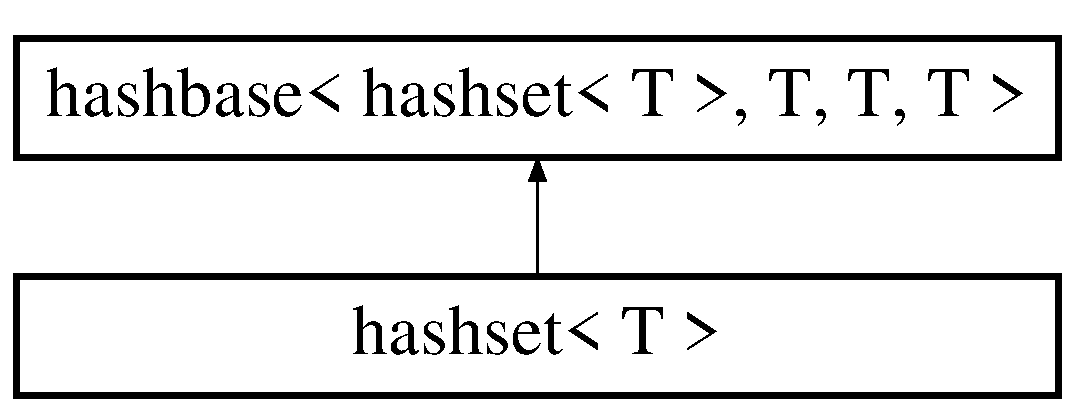
\includegraphics[height=2.000000cm]{structhashset}
\end{center}
\end{figure}
\subsection*{Public Types}
\begin{DoxyCompactItemize}
\item 
\mbox{\Hypertarget{structhashset_ae5d30803fe1cb2a38de47a93a0d9ed7a}\label{structhashset_ae5d30803fe1cb2a38de47a93a0d9ed7a}} 
typedef \hyperlink{structhashbase}{hashbase}$<$ \hyperlink{structhashset}{hashset}$<$ T $>$, T, T, T $>$ {\bfseries basetype}
\end{DoxyCompactItemize}
\subsection*{Public Member Functions}
\begin{DoxyCompactItemize}
\item 
\mbox{\Hypertarget{structhashset_a68388a2d354e5ea6bc8872248b888150}\label{structhashset_a68388a2d354e5ea6bc8872248b888150}} 
{\bfseries hashset} (int size=basetype\+::\+D\+E\+F\+A\+U\+L\+T\+S\+I\+ZE)
\end{DoxyCompactItemize}
\subsection*{Static Public Member Functions}
\begin{DoxyCompactItemize}
\item 
\mbox{\Hypertarget{structhashset_a2be80c77c4a0cefdfeaf41166dfea3d6}\label{structhashset_a2be80c77c4a0cefdfeaf41166dfea3d6}} 
static const T \& {\bfseries getkey} (const T \&elem)
\item 
\mbox{\Hypertarget{structhashset_ae34c3744742868fe30b9d5a25c793b25}\label{structhashset_ae34c3744742868fe30b9d5a25c793b25}} 
static T \& {\bfseries getdata} (T \&elem)
\item 
\mbox{\Hypertarget{structhashset_adb277a04e78c4730d3aeffb8f2c795c9}\label{structhashset_adb277a04e78c4730d3aeffb8f2c795c9}} 
{\footnotesize template$<$class K $>$ }\\static void {\bfseries setkey} (T \&elem, const K \&key)
\end{DoxyCompactItemize}
\subsection*{Additional Inherited Members}


The documentation for this struct was generated from the following file\+:\begin{DoxyCompactItemize}
\item 
H\+:/\+Rival\+Engine/\+Rival\+\_\+\+Game\+\_\+\+Engine\+\_\+\+G\+I\+T/\+Rival3dengine/source/shared/tools.\+h\end{DoxyCompactItemize}

\hypertarget{structhashtable}{}\section{hashtable$<$ K, T $>$ Struct Template Reference}
\label{structhashtable}\index{hashtable$<$ K, T $>$@{hashtable$<$ K, T $>$}}
Inheritance diagram for hashtable$<$ K, T $>$\+:\begin{figure}[H]
\begin{center}
\leavevmode
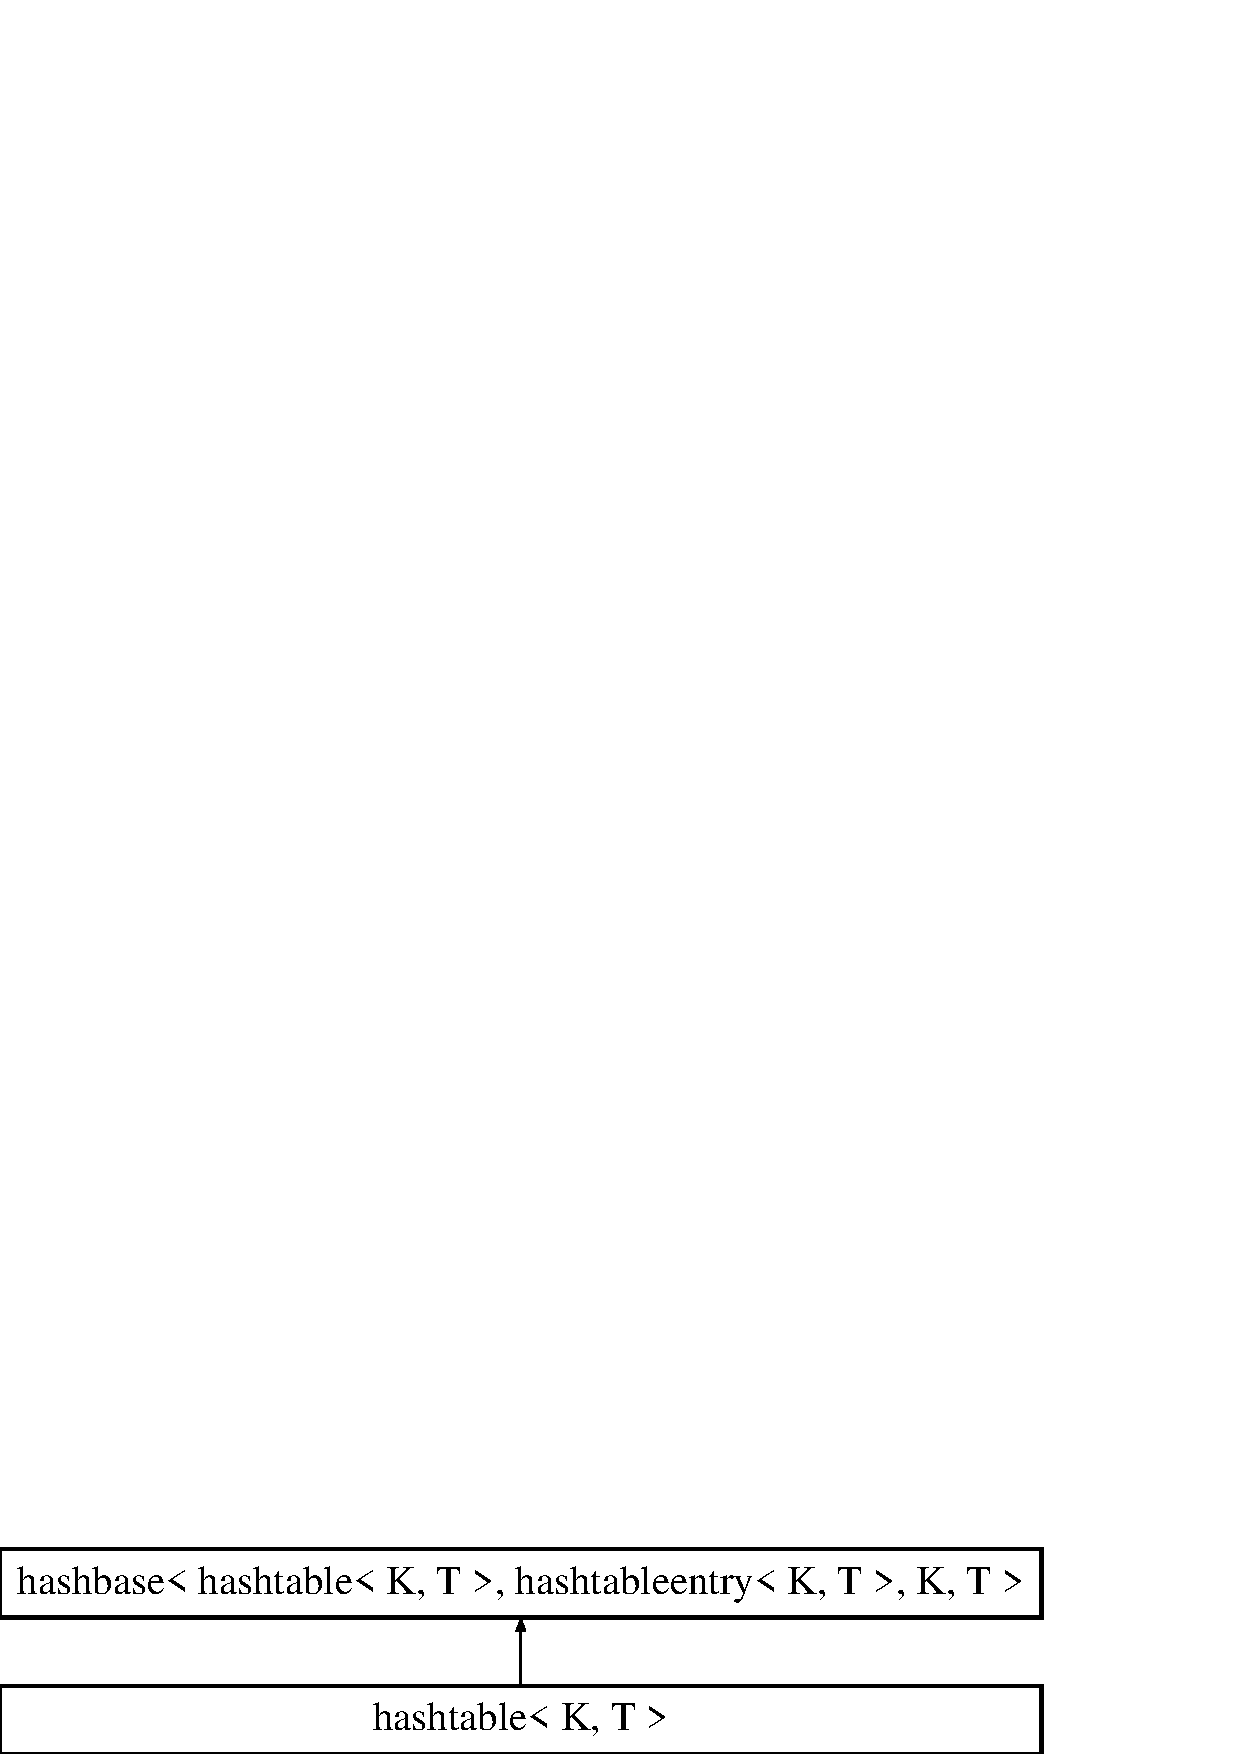
\includegraphics[height=2.000000cm]{structhashtable}
\end{center}
\end{figure}
\subsection*{Public Types}
\begin{DoxyCompactItemize}
\item 
\mbox{\Hypertarget{structhashtable_a6293bf03faedf41b5da3e61c55f165ce}\label{structhashtable_a6293bf03faedf41b5da3e61c55f165ce}} 
typedef \hyperlink{structhashbase}{hashbase}$<$ \hyperlink{structhashtable}{hashtable}$<$ K, T $>$, \hyperlink{structhashtableentry}{hashtableentry}$<$ K, T $>$, K, T $>$ {\bfseries basetype}
\item 
\mbox{\Hypertarget{structhashtable_aa17f663dc44e924ffb3d497d82cb5db9}\label{structhashtable_aa17f663dc44e924ffb3d497d82cb5db9}} 
typedef \hyperlink{structhashtableentry}{basetype\+::elemtype} {\bfseries elemtype}
\end{DoxyCompactItemize}
\subsection*{Public Member Functions}
\begin{DoxyCompactItemize}
\item 
\mbox{\Hypertarget{structhashtable_adb434ea3da2c1513ea38afb50fcf9e64}\label{structhashtable_adb434ea3da2c1513ea38afb50fcf9e64}} 
{\bfseries hashtable} (int size=basetype\+::\+D\+E\+F\+A\+U\+L\+T\+S\+I\+ZE)
\end{DoxyCompactItemize}
\subsection*{Static Public Member Functions}
\begin{DoxyCompactItemize}
\item 
\mbox{\Hypertarget{structhashtable_a8d0073175cc7bcf13bbafa1d95da9105}\label{structhashtable_a8d0073175cc7bcf13bbafa1d95da9105}} 
static K \& {\bfseries getkey} (\hyperlink{structhashtableentry}{elemtype} \&elem)
\item 
\mbox{\Hypertarget{structhashtable_aec9573e5c4052c0d78ab73750a000df8}\label{structhashtable_aec9573e5c4052c0d78ab73750a000df8}} 
static T \& {\bfseries getdata} (\hyperlink{structhashtableentry}{elemtype} \&elem)
\item 
\mbox{\Hypertarget{structhashtable_ac4d28d6bfb1fc1203ee98d648a32d53a}\label{structhashtable_ac4d28d6bfb1fc1203ee98d648a32d53a}} 
{\footnotesize template$<$class U $>$ }\\static void {\bfseries setkey} (\hyperlink{structhashtableentry}{elemtype} \&elem, const U \&key)
\end{DoxyCompactItemize}
\subsection*{Additional Inherited Members}


The documentation for this struct was generated from the following file\+:\begin{DoxyCompactItemize}
\item 
H\+:/\+Rival\+Engine/\+Rival\+\_\+\+Game\+\_\+\+Engine\+\_\+\+G\+I\+T/\+Rival3dengine/source/shared/tools.\+h\end{DoxyCompactItemize}

\hypertarget{structhashtableentry}{}\section{hashtableentry$<$ K, T $>$ Struct Template Reference}
\label{structhashtableentry}\index{hashtableentry$<$ K, T $>$@{hashtableentry$<$ K, T $>$}}
\subsection*{Public Attributes}
\begin{DoxyCompactItemize}
\item 
\mbox{\Hypertarget{structhashtableentry_ad882a0848d9cf60d65916707996b0789}\label{structhashtableentry_ad882a0848d9cf60d65916707996b0789}} 
K {\bfseries key}
\item 
\mbox{\Hypertarget{structhashtableentry_ac8b0c1b7a31e26f61f8eabdeffc5cf71}\label{structhashtableentry_ac8b0c1b7a31e26f61f8eabdeffc5cf71}} 
T {\bfseries data}
\end{DoxyCompactItemize}


The documentation for this struct was generated from the following file\+:\begin{DoxyCompactItemize}
\item 
H\+:/\+Rival\+Engine/\+Rival\+\_\+\+Game\+\_\+\+Engine\+\_\+\+G\+I\+T/\+Rival3dengine/source/shared/tools.\+h\end{DoxyCompactItemize}

\hypertarget{uniontiger_1_1hashval}{}\section{tiger\+:\+:hashval Union Reference}
\label{uniontiger_1_1hashval}\index{tiger\+::hashval@{tiger\+::hashval}}
\subsection*{Public Attributes}
\begin{DoxyCompactItemize}
\item 
\mbox{\Hypertarget{uniontiger_1_1hashval_a60762fc3ee7fc547c020f50966313e89}\label{uniontiger_1_1hashval_a60762fc3ee7fc547c020f50966313e89}} 
uchar {\bfseries bytes} \mbox{[}3 $\ast$8\mbox{]}
\item 
\mbox{\Hypertarget{uniontiger_1_1hashval_ac4b524d3ed4b6a1f60bf9f8ce493ecb5}\label{uniontiger_1_1hashval_ac4b524d3ed4b6a1f60bf9f8ce493ecb5}} 
chunk {\bfseries chunks} \mbox{[}3\mbox{]}
\end{DoxyCompactItemize}


The documentation for this union was generated from the following file\+:\begin{DoxyCompactItemize}
\item 
H\+:/\+Rival\+Engine/\+Rival\+\_\+\+Game\+\_\+\+Engine\+\_\+\+G\+I\+T/\+Rival3dengine/source/shared/crypto.\+cpp\end{DoxyCompactItemize}

\hypertarget{structserver_1_1hitinfo}{}\section{server\+:\+:hitinfo Struct Reference}
\label{structserver_1_1hitinfo}\index{server\+::hitinfo@{server\+::hitinfo}}
\subsection*{Public Attributes}
\begin{DoxyCompactItemize}
\item 
\mbox{\Hypertarget{structserver_1_1hitinfo_ae0b2bba1aa9cb4ec3bb47cc8a7e1d1c4}\label{structserver_1_1hitinfo_ae0b2bba1aa9cb4ec3bb47cc8a7e1d1c4}} 
int {\bfseries target}
\item 
\mbox{\Hypertarget{structserver_1_1hitinfo_abd4e9eb1ea0f47f7c3f0f526c70fed72}\label{structserver_1_1hitinfo_abd4e9eb1ea0f47f7c3f0f526c70fed72}} 
int {\bfseries lifesequence}
\item 
\mbox{\Hypertarget{structserver_1_1hitinfo_a65885ed25f26fff3286fc350a24a0cc6}\label{structserver_1_1hitinfo_a65885ed25f26fff3286fc350a24a0cc6}} 
int {\bfseries rays}
\item 
\mbox{\Hypertarget{structserver_1_1hitinfo_a08df7d270caa963abc92dd648f8b3017}\label{structserver_1_1hitinfo_a08df7d270caa963abc92dd648f8b3017}} 
float {\bfseries dist}
\item 
\mbox{\Hypertarget{structserver_1_1hitinfo_acf74f83c8efebb6e9f7d95e932287206}\label{structserver_1_1hitinfo_acf74f83c8efebb6e9f7d95e932287206}} 
\hyperlink{structvec}{vec} {\bfseries dir}
\end{DoxyCompactItemize}


The documentation for this struct was generated from the following file\+:\begin{DoxyCompactItemize}
\item 
H\+:/\+Rival\+Engine/\+Rival\+\_\+\+Game\+\_\+\+Engine\+\_\+\+G\+I\+T/\+Rival3dengine/source/game/server.\+cpp\end{DoxyCompactItemize}

\hypertarget{structgame_1_1hitmsg}{}\section{game\+:\+:hitmsg Struct Reference}
\label{structgame_1_1hitmsg}\index{game\+::hitmsg@{game\+::hitmsg}}
\subsection*{Public Attributes}
\begin{DoxyCompactItemize}
\item 
\mbox{\Hypertarget{structgame_1_1hitmsg_a39030a03de0769ae6ba01a55d0760947}\label{structgame_1_1hitmsg_a39030a03de0769ae6ba01a55d0760947}} 
int {\bfseries target}
\item 
\mbox{\Hypertarget{structgame_1_1hitmsg_ae0e50d30529254a84ed15ac6e4c83f3b}\label{structgame_1_1hitmsg_ae0e50d30529254a84ed15ac6e4c83f3b}} 
int {\bfseries lifesequence}
\item 
\mbox{\Hypertarget{structgame_1_1hitmsg_afcd8c00a4694074318e8f4b3f3f4883c}\label{structgame_1_1hitmsg_afcd8c00a4694074318e8f4b3f3f4883c}} 
int {\bfseries info1}
\item 
\mbox{\Hypertarget{structgame_1_1hitmsg_ad1e24e2ec1f2f0008e6638cc733b019d}\label{structgame_1_1hitmsg_ad1e24e2ec1f2f0008e6638cc733b019d}} 
int {\bfseries info2}
\item 
\mbox{\Hypertarget{structgame_1_1hitmsg_a78314fb24d3f864ef72059cfa7a7d400}\label{structgame_1_1hitmsg_a78314fb24d3f864ef72059cfa7a7d400}} 
\hyperlink{structivec}{ivec} {\bfseries dir}
\end{DoxyCompactItemize}


The documentation for this struct was generated from the following file\+:\begin{DoxyCompactItemize}
\item 
H\+:/\+Rival\+Engine/\+Rival\+\_\+\+Game\+\_\+\+Engine\+\_\+\+G\+I\+T/\+Rival3dengine/source/game/weapon.\+cpp\end{DoxyCompactItemize}

\hypertarget{structhline}{}\section{hline Struct Reference}
\label{structhline}\index{hline@{hline}}
\subsection*{Public Member Functions}
\begin{DoxyCompactItemize}
\item 
\mbox{\Hypertarget{structhline_ad2a9ef66a6061ea45769648c808f034a}\label{structhline_ad2a9ef66a6061ea45769648c808f034a}} 
void {\bfseries restore} ()
\item 
\mbox{\Hypertarget{structhline_afe7c38d5d1b78f1b5b3fa5a2be7ef58e}\label{structhline_afe7c38d5d1b78f1b5b3fa5a2be7ef58e}} 
bool {\bfseries shouldsave} ()
\item 
\mbox{\Hypertarget{structhline_a46879d386c77eaa14f750b2a87d9dfa8}\label{structhline_a46879d386c77eaa14f750b2a87d9dfa8}} 
void {\bfseries save} ()
\item 
\mbox{\Hypertarget{structhline_a73e39715f56187b48bb69d865a4eb18d}\label{structhline_a73e39715f56187b48bb69d865a4eb18d}} 
void {\bfseries run} ()
\end{DoxyCompactItemize}
\subsection*{Public Attributes}
\begin{DoxyCompactItemize}
\item 
\mbox{\Hypertarget{structhline_a3d5eb6c5052790925e02003e0896f920}\label{structhline_a3d5eb6c5052790925e02003e0896f920}} 
char $\ast$ {\bfseries buf}
\item 
\mbox{\Hypertarget{structhline_af973bce10839b024a41054df855fa10a}\label{structhline_af973bce10839b024a41054df855fa10a}} 
char $\ast$ {\bfseries action}
\item 
\mbox{\Hypertarget{structhline_a466a5dc0d8578feadd710810deac243e}\label{structhline_a466a5dc0d8578feadd710810deac243e}} 
char $\ast$ {\bfseries prompt}
\item 
\mbox{\Hypertarget{structhline_ad6e9f92b194a27547e5fd435f58549f4}\label{structhline_ad6e9f92b194a27547e5fd435f58549f4}} 
int {\bfseries flags}
\end{DoxyCompactItemize}


The documentation for this struct was generated from the following file\+:\begin{DoxyCompactItemize}
\item 
H\+:/\+Rival\+Engine/\+Rival\+\_\+\+Game\+\_\+\+Engine\+\_\+\+G\+I\+T/\+Rival3dengine/source/engine/console.\+cpp\end{DoxyCompactItemize}

\hypertarget{struct_u_i_1_1_horizontal_list}{}\section{UI\+:\+:Horizontal\+List Struct Reference}
\label{struct_u_i_1_1_horizontal_list}\index{U\+I\+::\+Horizontal\+List@{U\+I\+::\+Horizontal\+List}}
Inheritance diagram for UI\+:\+:Horizontal\+List\+:\begin{figure}[H]
\begin{center}
\leavevmode
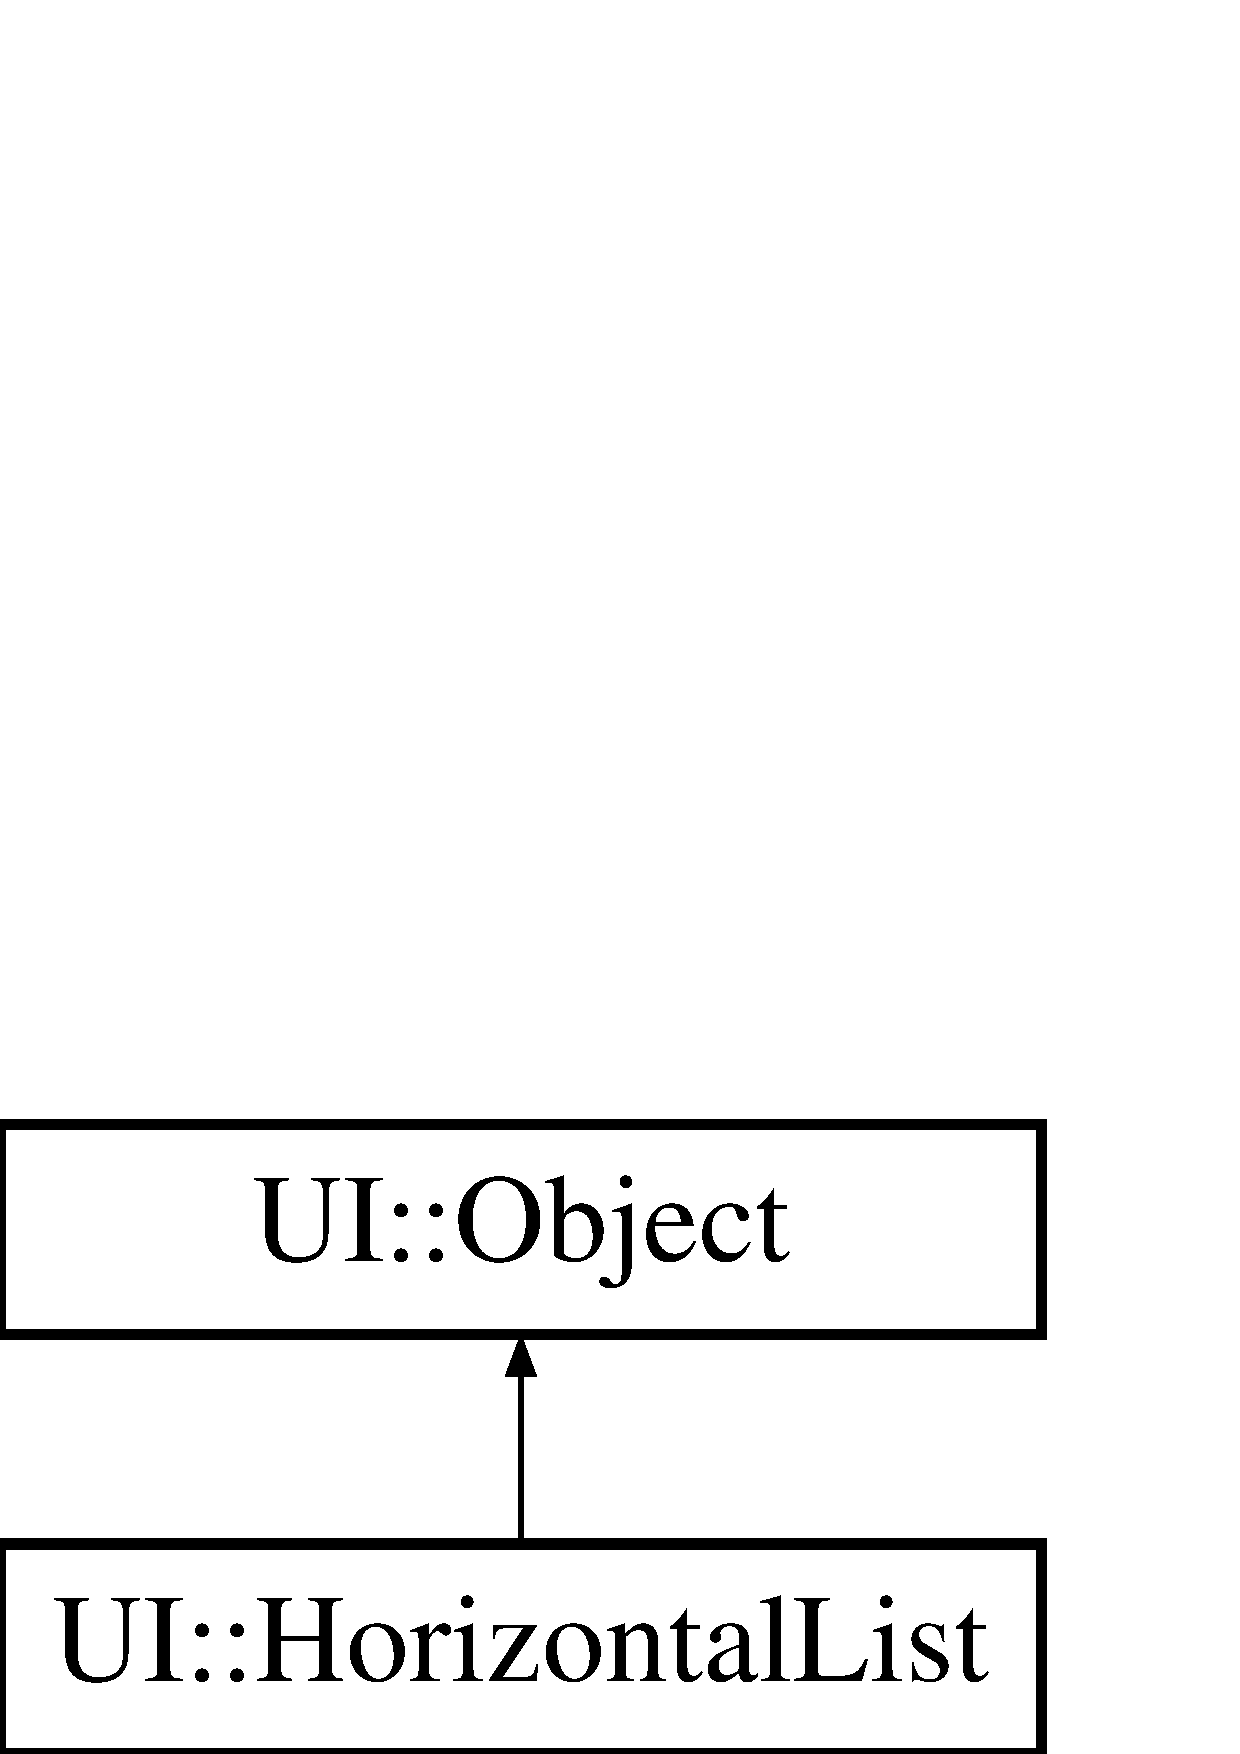
\includegraphics[height=2.000000cm]{struct_u_i_1_1_horizontal_list}
\end{center}
\end{figure}
\subsection*{Public Member Functions}
\begin{DoxyCompactItemize}
\item 
\mbox{\Hypertarget{struct_u_i_1_1_horizontal_list_a69a91132a6a618aa77552e9cd73c1291}\label{struct_u_i_1_1_horizontal_list_a69a91132a6a618aa77552e9cd73c1291}} 
const char $\ast$ {\bfseries gettype} () const
\item 
\mbox{\Hypertarget{struct_u_i_1_1_horizontal_list_affdd0a8d912b7a1148009d2b622ccb28}\label{struct_u_i_1_1_horizontal_list_affdd0a8d912b7a1148009d2b622ccb28}} 
void {\bfseries setup} (float space\+\_\+=0)
\item 
\mbox{\Hypertarget{struct_u_i_1_1_horizontal_list_a7d9401d953278d6e6b4bf0c708be0c42}\label{struct_u_i_1_1_horizontal_list_a7d9401d953278d6e6b4bf0c708be0c42}} 
uchar {\bfseries childalign} () const
\item 
\mbox{\Hypertarget{struct_u_i_1_1_horizontal_list_aed6633bc0e9bff0267061f9ba8c21fb8}\label{struct_u_i_1_1_horizontal_list_aed6633bc0e9bff0267061f9ba8c21fb8}} 
void {\bfseries layout} ()
\item 
\mbox{\Hypertarget{struct_u_i_1_1_horizontal_list_a4d4d6afe27986727407857dcf1420332}\label{struct_u_i_1_1_horizontal_list_a4d4d6afe27986727407857dcf1420332}} 
void {\bfseries adjustchildren} ()
\end{DoxyCompactItemize}
\subsection*{Static Public Member Functions}
\begin{DoxyCompactItemize}
\item 
\mbox{\Hypertarget{struct_u_i_1_1_horizontal_list_af18d7e314bb8eb16e2a1bd93953cc4fa}\label{struct_u_i_1_1_horizontal_list_af18d7e314bb8eb16e2a1bd93953cc4fa}} 
static const char $\ast$ {\bfseries typestr} ()
\end{DoxyCompactItemize}
\subsection*{Public Attributes}
\begin{DoxyCompactItemize}
\item 
\mbox{\Hypertarget{struct_u_i_1_1_horizontal_list_a57e0e7fc094d5d4f7a19d90d5fb9529d}\label{struct_u_i_1_1_horizontal_list_a57e0e7fc094d5d4f7a19d90d5fb9529d}} 
float {\bfseries space}
\item 
\mbox{\Hypertarget{struct_u_i_1_1_horizontal_list_aaf20c385cd68973db7ee04ae1686d88e}\label{struct_u_i_1_1_horizontal_list_aaf20c385cd68973db7ee04ae1686d88e}} 
float {\bfseries subw}
\end{DoxyCompactItemize}


The documentation for this struct was generated from the following file\+:\begin{DoxyCompactItemize}
\item 
H\+:/\+Rival\+Engine/\+Rival\+\_\+\+Game\+\_\+\+Engine\+\_\+\+G\+I\+T/\+Rival3dengine/source/engine/ui.\+cpp\end{DoxyCompactItemize}

\hypertarget{struct_u_i_1_1_horizontal_scroll_bar}{}\section{UI\+:\+:Horizontal\+Scroll\+Bar Struct Reference}
\label{struct_u_i_1_1_horizontal_scroll_bar}\index{U\+I\+::\+Horizontal\+Scroll\+Bar@{U\+I\+::\+Horizontal\+Scroll\+Bar}}
Inheritance diagram for UI\+:\+:Horizontal\+Scroll\+Bar\+:\begin{figure}[H]
\begin{center}
\leavevmode
\includegraphics[height=3.000000cm]{struct_u_i_1_1_horizontal_scroll_bar}
\end{center}
\end{figure}
\subsection*{Public Member Functions}
\begin{DoxyCompactItemize}
\item 
\mbox{\Hypertarget{struct_u_i_1_1_horizontal_scroll_bar_a9de677a31bbc314b7c6ee7fd9f80072a}\label{struct_u_i_1_1_horizontal_scroll_bar_a9de677a31bbc314b7c6ee7fd9f80072a}} 
const char $\ast$ {\bfseries gettype} () const
\item 
\mbox{\Hypertarget{struct_u_i_1_1_horizontal_scroll_bar_a6231ad5e3e4b9ec8d5e277173884fab2}\label{struct_u_i_1_1_horizontal_scroll_bar_a6231ad5e3e4b9ec8d5e277173884fab2}} 
void {\bfseries addscroll} (\hyperlink{struct_u_i_1_1_scroller}{Scroller} $\ast$scroller, float dir)
\item 
\mbox{\Hypertarget{struct_u_i_1_1_horizontal_scroll_bar_a3ec3496b8af45fa3ba62cf9f7265140b}\label{struct_u_i_1_1_horizontal_scroll_bar_a3ec3496b8af45fa3ba62cf9f7265140b}} 
void {\bfseries scrollto} (float cx, float cy, bool closest=false)
\item 
\mbox{\Hypertarget{struct_u_i_1_1_horizontal_scroll_bar_a6952cb698f8aee022684fe4411f5dfa5}\label{struct_u_i_1_1_horizontal_scroll_bar_a6952cb698f8aee022684fe4411f5dfa5}} 
void {\bfseries adjustchildren} ()
\item 
\mbox{\Hypertarget{struct_u_i_1_1_horizontal_scroll_bar_a18488ff0a4faf7f36202630c96adc055}\label{struct_u_i_1_1_horizontal_scroll_bar_a18488ff0a4faf7f36202630c96adc055}} 
void {\bfseries movebutton} (\hyperlink{struct_u_i_1_1_object}{Object} $\ast$o, float fromx, float fromy, float tox, float toy)
\end{DoxyCompactItemize}
\subsection*{Static Public Member Functions}
\begin{DoxyCompactItemize}
\item 
\mbox{\Hypertarget{struct_u_i_1_1_horizontal_scroll_bar_a5527a592d5594de104fc930872017fe7}\label{struct_u_i_1_1_horizontal_scroll_bar_a5527a592d5594de104fc930872017fe7}} 
static const char $\ast$ {\bfseries typestr} ()
\end{DoxyCompactItemize}
\subsection*{Additional Inherited Members}


The documentation for this struct was generated from the following file\+:\begin{DoxyCompactItemize}
\item 
H\+:/\+Rival\+Engine/\+Rival\+\_\+\+Game\+\_\+\+Engine\+\_\+\+G\+I\+T/\+Rival3dengine/source/engine/ui.\+cpp\end{DoxyCompactItemize}

\hypertarget{struct_u_i_1_1_horizontal_slider}{}\section{UI\+:\+:Horizontal\+Slider Struct Reference}
\label{struct_u_i_1_1_horizontal_slider}\index{U\+I\+::\+Horizontal\+Slider@{U\+I\+::\+Horizontal\+Slider}}
Inheritance diagram for UI\+:\+:Horizontal\+Slider\+:\begin{figure}[H]
\begin{center}
\leavevmode
\includegraphics[height=3.000000cm]{struct_u_i_1_1_horizontal_slider}
\end{center}
\end{figure}
\subsection*{Public Member Functions}
\begin{DoxyCompactItemize}
\item 
\mbox{\Hypertarget{struct_u_i_1_1_horizontal_slider_af87c8724ef136e4f8569e1b5beac44eb}\label{struct_u_i_1_1_horizontal_slider_af87c8724ef136e4f8569e1b5beac44eb}} 
const char $\ast$ {\bfseries gettype} () const
\item 
\mbox{\Hypertarget{struct_u_i_1_1_horizontal_slider_acdf7ba34ff12cc1f0786e51f00e77a35}\label{struct_u_i_1_1_horizontal_slider_acdf7ba34ff12cc1f0786e51f00e77a35}} 
void {\bfseries scrollto} (float cx, float cy)
\item 
\mbox{\Hypertarget{struct_u_i_1_1_horizontal_slider_ab4b39bf682c1f025f4fde682decfd859}\label{struct_u_i_1_1_horizontal_slider_ab4b39bf682c1f025f4fde682decfd859}} 
void {\bfseries adjustchildren} ()
\end{DoxyCompactItemize}
\subsection*{Static Public Member Functions}
\begin{DoxyCompactItemize}
\item 
\mbox{\Hypertarget{struct_u_i_1_1_horizontal_slider_a782b1a63b40e374106e60e56cb0a71e3}\label{struct_u_i_1_1_horizontal_slider_a782b1a63b40e374106e60e56cb0a71e3}} 
static const char $\ast$ {\bfseries typestr} ()
\end{DoxyCompactItemize}
\subsection*{Additional Inherited Members}


The documentation for this struct was generated from the following file\+:\begin{DoxyCompactItemize}
\item 
H\+:/\+Rival\+Engine/\+Rival\+\_\+\+Game\+\_\+\+Engine\+\_\+\+G\+I\+T/\+Rival3dengine/source/engine/ui.\+cpp\end{DoxyCompactItemize}

\hypertarget{structgame_1_1hudent}{}\section{game\+:\+:hudent Struct Reference}
\label{structgame_1_1hudent}\index{game\+::hudent@{game\+::hudent}}
Inheritance diagram for game\+:\+:hudent\+:\begin{figure}[H]
\begin{center}
\leavevmode
\includegraphics[height=3.000000cm]{structgame_1_1hudent}
\end{center}
\end{figure}
\subsection*{Additional Inherited Members}


The documentation for this struct was generated from the following file\+:\begin{DoxyCompactItemize}
\item 
H\+:/\+Rival\+Engine/\+Rival\+\_\+\+Game\+\_\+\+Engine\+\_\+\+G\+I\+T/\+Rival3dengine/source/game/render.\+cpp\end{DoxyCompactItemize}

\hypertarget{structhvec}{}\section{hvec Struct Reference}
\label{structhvec}\index{hvec@{hvec}}
\subsection*{Public Member Functions}
\begin{DoxyCompactItemize}
\item 
\mbox{\Hypertarget{structhvec_aa650da33f299cb90d066f877a3a96065}\label{structhvec_aa650da33f299cb90d066f877a3a96065}} 
{\footnotesize template$<$class T $>$ }\\{\bfseries hvec} (T x, T y, T z)
\item 
\mbox{\Hypertarget{structhvec_a6fab7b143c957155f4e2697814b46760}\label{structhvec_a6fab7b143c957155f4e2697814b46760}} 
{\bfseries hvec} (const \hyperlink{structvec}{vec} \&v)
\item 
\mbox{\Hypertarget{structhvec_ae51670acb58d2638e17a9738686c9582}\label{structhvec_ae51670acb58d2638e17a9738686c9582}} 
bool {\bfseries operator==} (const \hyperlink{structhvec}{hvec} \&h) const
\item 
\mbox{\Hypertarget{structhvec_aa7ed4f97334561babfd9c1b4f2c1e3d5}\label{structhvec_aa7ed4f97334561babfd9c1b4f2c1e3d5}} 
bool {\bfseries operator!=} (const \hyperlink{structhvec}{hvec} \&h) const
\end{DoxyCompactItemize}
\subsection*{Public Attributes}
\begin{DoxyCompactItemize}
\item 
\mbox{\Hypertarget{structhvec_a0111d3ac72a5cd332a3a2e48b9d37dba}\label{structhvec_a0111d3ac72a5cd332a3a2e48b9d37dba}} 
\hyperlink{structhalf}{half} {\bfseries x}
\item 
\mbox{\Hypertarget{structhvec_aa5026a756662397dbf79f86fee25842e}\label{structhvec_aa5026a756662397dbf79f86fee25842e}} 
\hyperlink{structhalf}{half} {\bfseries y}
\item 
\mbox{\Hypertarget{structhvec_a856b4204264a20cbe2a579a61ce63561}\label{structhvec_a856b4204264a20cbe2a579a61ce63561}} 
\hyperlink{structhalf}{half} {\bfseries z}
\end{DoxyCompactItemize}


The documentation for this struct was generated from the following file\+:\begin{DoxyCompactItemize}
\item 
H\+:/\+Rival\+Engine/\+Rival\+\_\+\+Game\+\_\+\+Engine\+\_\+\+G\+I\+T/\+Rival3dengine/source/shared/geom.\+h\end{DoxyCompactItemize}

\hypertarget{structhvec2}{}\section{hvec2 Struct Reference}
\label{structhvec2}\index{hvec2@{hvec2}}
\subsection*{Public Member Functions}
\begin{DoxyCompactItemize}
\item 
\mbox{\Hypertarget{structhvec2_a883b7e3fbd94e228f77e850285b530b2}\label{structhvec2_a883b7e3fbd94e228f77e850285b530b2}} 
{\footnotesize template$<$class T $>$ }\\{\bfseries hvec2} (T x, T y)
\item 
\mbox{\Hypertarget{structhvec2_a9f6a5ffe185884df529de979bf500c2e}\label{structhvec2_a9f6a5ffe185884df529de979bf500c2e}} 
{\bfseries hvec2} (const \hyperlink{structvec2}{vec2} \&v)
\item 
\mbox{\Hypertarget{structhvec2_a73e3c8a3fcd2fcc222474c11247c2b82}\label{structhvec2_a73e3c8a3fcd2fcc222474c11247c2b82}} 
bool {\bfseries operator==} (const \hyperlink{structhvec2}{hvec2} \&h) const
\item 
\mbox{\Hypertarget{structhvec2_a5f48efd2c5e3e8e849f4e9b4831c1b43}\label{structhvec2_a5f48efd2c5e3e8e849f4e9b4831c1b43}} 
bool {\bfseries operator!=} (const \hyperlink{structhvec2}{hvec2} \&h) const
\end{DoxyCompactItemize}
\subsection*{Public Attributes}
\begin{DoxyCompactItemize}
\item 
\mbox{\Hypertarget{structhvec2_aecc105cd988f8bf1aeac2a1b74b051cd}\label{structhvec2_aecc105cd988f8bf1aeac2a1b74b051cd}} 
\hyperlink{structhalf}{half} {\bfseries x}
\item 
\mbox{\Hypertarget{structhvec2_a6f7c34724f31ba004fef6f5eecca972f}\label{structhvec2_a6f7c34724f31ba004fef6f5eecca972f}} 
\hyperlink{structhalf}{half} {\bfseries y}
\end{DoxyCompactItemize}


The documentation for this struct was generated from the following file\+:\begin{DoxyCompactItemize}
\item 
H\+:/\+Rival\+Engine/\+Rival\+\_\+\+Game\+\_\+\+Engine\+\_\+\+G\+I\+T/\+Rival3dengine/source/shared/geom.\+h\end{DoxyCompactItemize}

\hypertarget{structhvec4}{}\section{hvec4 Struct Reference}
\label{structhvec4}\index{hvec4@{hvec4}}
\subsection*{Public Member Functions}
\begin{DoxyCompactItemize}
\item 
\mbox{\Hypertarget{structhvec4_a651c521f28594966b1480cd2f8989932}\label{structhvec4_a651c521f28594966b1480cd2f8989932}} 
{\footnotesize template$<$class T $>$ }\\{\bfseries hvec4} (T x, T y, T z, T w)
\item 
\mbox{\Hypertarget{structhvec4_abea40299a905d039dd2ab4a1c01e6eed}\label{structhvec4_abea40299a905d039dd2ab4a1c01e6eed}} 
{\footnotesize template$<$class T $>$ }\\{\bfseries hvec4} (const \hyperlink{structvec}{vec} \&v, T w=0)
\item 
\mbox{\Hypertarget{structhvec4_a501c10fb8668699de9d01b860c89f969}\label{structhvec4_a501c10fb8668699de9d01b860c89f969}} 
{\bfseries hvec4} (const \hyperlink{structvec4}{vec4} \&v)
\item 
\mbox{\Hypertarget{structhvec4_a3b786e194c39501364ab3b797ace36e6}\label{structhvec4_a3b786e194c39501364ab3b797ace36e6}} 
bool {\bfseries operator==} (const \hyperlink{structhvec4}{hvec4} \&h) const
\item 
\mbox{\Hypertarget{structhvec4_a6cdea4e790c60b1e7b816307ba6edb1a}\label{structhvec4_a6cdea4e790c60b1e7b816307ba6edb1a}} 
bool {\bfseries operator!=} (const \hyperlink{structhvec4}{hvec4} \&h) const
\end{DoxyCompactItemize}
\subsection*{Public Attributes}
\begin{DoxyCompactItemize}
\item 
\mbox{\Hypertarget{structhvec4_a556817483babaaa77d112337b17ec1d8}\label{structhvec4_a556817483babaaa77d112337b17ec1d8}} 
\hyperlink{structhalf}{half} {\bfseries x}
\item 
\mbox{\Hypertarget{structhvec4_a5450248ae2dcd735d11f3d03a1ff0d3a}\label{structhvec4_a5450248ae2dcd735d11f3d03a1ff0d3a}} 
\hyperlink{structhalf}{half} {\bfseries y}
\item 
\mbox{\Hypertarget{structhvec4_aea76478717c70b2afb21dbd30b52d336}\label{structhvec4_aea76478717c70b2afb21dbd30b52d336}} 
\hyperlink{structhalf}{half} {\bfseries z}
\item 
\mbox{\Hypertarget{structhvec4_a7e7f44da8606820ebbceb96791689d80}\label{structhvec4_a7e7f44da8606820ebbceb96791689d80}} 
\hyperlink{structhalf}{half} {\bfseries w}
\end{DoxyCompactItemize}


The documentation for this struct was generated from the following file\+:\begin{DoxyCompactItemize}
\item 
H\+:/\+Rival\+Engine/\+Rival\+\_\+\+Game\+\_\+\+Engine\+\_\+\+G\+I\+T/\+Rival3dengine/source/shared/geom.\+h\end{DoxyCompactItemize}

\hypertarget{struct_i_controller}{}\section{I\+Controller Struct Reference}
\label{struct_i_controller}\index{I\+Controller@{I\+Controller}}
\subsection*{Public Attributes}
\begin{DoxyCompactItemize}
\item 
\mbox{\Hypertarget{struct_i_controller_a62f909fdab19d025eaf3967997b3fd6a}\label{struct_i_controller_a62f909fdab19d025eaf3967997b3fd6a}} 
int {\bfseries a}
\item 
\mbox{\Hypertarget{struct_i_controller_ad17ab0aaef1830552b6d9d4e8352a4ed}\label{struct_i_controller_ad17ab0aaef1830552b6d9d4e8352a4ed}} 
\hyperlink{structnode}{node} $\ast$ {\bfseries self}
\end{DoxyCompactItemize}


The documentation for this struct was generated from the following file\+:\begin{DoxyCompactItemize}
\item 
H\+:/\+Rival\+Engine/\+Rival\+\_\+\+Game\+\_\+\+Engine\+\_\+\+G\+I\+T/\+Rival3dengine/source/engine/halo.\+h\end{DoxyCompactItemize}

\hypertarget{structident}{}\section{ident Struct Reference}
\label{structident}\index{ident@{ident}}
\subsection*{Public Member Functions}
\begin{DoxyCompactItemize}
\item 
\mbox{\Hypertarget{structident_aed8235d056f71c15a2c80fac76e396f7}\label{structident_aed8235d056f71c15a2c80fac76e396f7}} 
{\bfseries ident} (int t, const char $\ast$n, int m, int x, int $\ast$s, void $\ast$f=N\+U\+LL, int flags=0)
\item 
\mbox{\Hypertarget{structident_aee755c48ba698470423295660ca13c09}\label{structident_aee755c48ba698470423295660ca13c09}} 
{\bfseries ident} (int t, const char $\ast$n, float m, float x, float $\ast$s, void $\ast$f=N\+U\+LL, int flags=0)
\item 
\mbox{\Hypertarget{structident_a6cdba7cea1decd2b8790ebad42bc148b}\label{structident_a6cdba7cea1decd2b8790ebad42bc148b}} 
{\bfseries ident} (int t, const char $\ast$n, char $\ast$$\ast$s, void $\ast$f=N\+U\+LL, int flags=0)
\item 
\mbox{\Hypertarget{structident_a688f3403b66806f95638c925f5afe86f}\label{structident_a688f3403b66806f95638c925f5afe86f}} 
{\bfseries ident} (int t, const char $\ast$n, char $\ast$a, int flags)
\item 
\mbox{\Hypertarget{structident_af9c556cc1a34d2cbe8770cdf54ebb5b7}\label{structident_af9c556cc1a34d2cbe8770cdf54ebb5b7}} 
{\bfseries ident} (int t, const char $\ast$n, int a, int flags)
\item 
\mbox{\Hypertarget{structident_a43de4850c38c08928eea93b4c986c69b}\label{structident_a43de4850c38c08928eea93b4c986c69b}} 
{\bfseries ident} (int t, const char $\ast$n, float a, int flags)
\item 
\mbox{\Hypertarget{structident_a38f2de1252ef46f06e817d06d0de0136}\label{structident_a38f2de1252ef46f06e817d06d0de0136}} 
{\bfseries ident} (int t, const char $\ast$n, int flags)
\item 
\mbox{\Hypertarget{structident_ac680cb604154989900b58f26821113e8}\label{structident_ac680cb604154989900b58f26821113e8}} 
{\bfseries ident} (int t, const char $\ast$n, const \hyperlink{structtagval}{tagval} \&v, int flags)
\item 
\mbox{\Hypertarget{structident_aecef47728629977d84b86bd7b4d0461e}\label{structident_aecef47728629977d84b86bd7b4d0461e}} 
{\bfseries ident} (int t, const char $\ast$n, const char $\ast$args, uint argmask, int numargs, void $\ast$f=N\+U\+LL, int flags=0)
\item 
\mbox{\Hypertarget{structident_a2987d0a13aa0f742fce35433e0afaeb4}\label{structident_a2987d0a13aa0f742fce35433e0afaeb4}} 
void {\bfseries changed} ()
\item 
\mbox{\Hypertarget{structident_ad7d31a36f064ca0c13e86e2188a40958}\label{structident_ad7d31a36f064ca0c13e86e2188a40958}} 
void {\bfseries setval} (const \hyperlink{structtagval}{tagval} \&v)
\item 
\mbox{\Hypertarget{structident_a3c76c834540ff64f63fce96851b7a2e6}\label{structident_a3c76c834540ff64f63fce96851b7a2e6}} 
void {\bfseries setval} (const \hyperlink{structidentstack}{identstack} \&v)
\item 
\mbox{\Hypertarget{structident_a2388d38e1443832808604d4510589813}\label{structident_a2388d38e1443832808604d4510589813}} 
void {\bfseries forcenull} ()
\item 
\mbox{\Hypertarget{structident_a3e99fe01fda196cbe595b36d228c5c57}\label{structident_a3e99fe01fda196cbe595b36d228c5c57}} 
float {\bfseries getfloat} () const
\item 
\mbox{\Hypertarget{structident_a6ee21ad2fcf13a73bde77f8817cbbad1}\label{structident_a6ee21ad2fcf13a73bde77f8817cbbad1}} 
int {\bfseries getint} () const
\item 
\mbox{\Hypertarget{structident_a13a73126107fe2e347e03f325de8351e}\label{structident_a13a73126107fe2e347e03f325de8351e}} 
double {\bfseries getnumber} () const
\item 
\mbox{\Hypertarget{structident_a4cfcdd953809250886fdf2b4f6bb54a2}\label{structident_a4cfcdd953809250886fdf2b4f6bb54a2}} 
const char $\ast$ {\bfseries getstr} () const
\item 
\mbox{\Hypertarget{structident_aed50617b180326d483b62d5029187b41}\label{structident_aed50617b180326d483b62d5029187b41}} 
void {\bfseries getval} (\hyperlink{structtagval}{tagval} \&r) const
\item 
\mbox{\Hypertarget{structident_a97c7b12d58673a4c220e2fcc19a42cd8}\label{structident_a97c7b12d58673a4c220e2fcc19a42cd8}} 
void {\bfseries getcstr} (\hyperlink{structtagval}{tagval} \&v) const
\item 
\mbox{\Hypertarget{structident_adcc685bac610969c7e6f7e4483a72bc5}\label{structident_adcc685bac610969c7e6f7e4483a72bc5}} 
void {\bfseries getcval} (\hyperlink{structtagval}{tagval} \&v) const
\end{DoxyCompactItemize}
\subsection*{Public Attributes}
\begin{DoxyCompactItemize}
\item 
\mbox{\Hypertarget{structident_a89f53b6ecbddf478efd372ffe0ae6eda}\label{structident_a89f53b6ecbddf478efd372ffe0ae6eda}} 
uchar {\bfseries type}
\item 
\mbox{\Hypertarget{structident_af3d1413531f5a88b55ff6826eea9cbc0}\label{structident_af3d1413531f5a88b55ff6826eea9cbc0}} 
\begin{tabbing}
xx\=xx\=xx\=xx\=xx\=xx\=xx\=xx\=xx\=\kill
union \{\\
\>uchar {\bfseries valtype}\\
\>uchar {\bfseries numargs}\\
\}; \\

\end{tabbing}\item 
\mbox{\Hypertarget{structident_a784e8d5226f1bbb3d409540dc86020cb}\label{structident_a784e8d5226f1bbb3d409540dc86020cb}} 
ushort {\bfseries flags}
\item 
\mbox{\Hypertarget{structident_a059957b9554f4ad69d8781d6b7303799}\label{structident_a059957b9554f4ad69d8781d6b7303799}} 
int {\bfseries index}
\item 
\mbox{\Hypertarget{structident_a28ad74a961db36107528b12fb9b5e763}\label{structident_a28ad74a961db36107528b12fb9b5e763}} 
const char $\ast$ {\bfseries name}
\item 
\mbox{\Hypertarget{structident_aefff1767257e119616ee4f35b0d2c140}\label{structident_aefff1767257e119616ee4f35b0d2c140}} 
\begin{tabbing}
xx\=xx\=xx\=xx\=xx\=xx\=xx\=xx\=xx\=\kill
union \{\\
\mbox{\Hypertarget{unionident_1_1_0D148_a0e53b26c2089cccf9c337d334331a91d}\label{unionident_1_1_0D148_a0e53b26c2089cccf9c337d334331a91d}} 
\>struct \{\\
\mbox{\Hypertarget{structident_1_1_0D148_1_1_0D150_aaa083655f49c5f6034495198dba59235}\label{structident_1_1_0D148_1_1_0D150_aaa083655f49c5f6034495198dba59235}} 
\>\>union \{\\
\mbox{\Hypertarget{unionident_1_1_0D148_1_1_0D150_1_1_0D156_a9ef967637a7c8857f0d59188e75d8aed}\label{unionident_1_1_0D148_1_1_0D150_1_1_0D156_a9ef967637a7c8857f0d59188e75d8aed}} 
\>\>\>struct \{\\
\>\>\>\>int {\bfseries minval}\\
\>\>\>\>int {\bfseries maxval}\\
\>\>\>\} \\
\mbox{\Hypertarget{unionident_1_1_0D148_1_1_0D150_1_1_0D156_ab12a0b5d20f70363a642e23f7a111055}\label{unionident_1_1_0D148_1_1_0D150_1_1_0D156_ab12a0b5d20f70363a642e23f7a111055}} 
\>\>\>struct \{\\
\>\>\>\>float {\bfseries minvalf}\\
\>\>\>\>float {\bfseries maxvalf}\\
\>\>\>\} \\
\>\>\} \\
\>\>\hyperlink{unionidentvalptr}{identvalptr} {\bfseries storage}\\
\>\>\hyperlink{structidentval}{identval} {\bfseries overrideval}\\
\>\} \\
\mbox{\Hypertarget{unionident_1_1_0D148_a29cb0d517cd02797fcc6f5b367e1c01f}\label{unionident_1_1_0D148_a29cb0d517cd02797fcc6f5b367e1c01f}} 
\>struct \{\\
\>\>uint $\ast$ {\bfseries code}\\
\>\>\hyperlink{structidentval}{identval} {\bfseries val}\\
\>\>\hyperlink{structidentstack}{identstack} $\ast$ {\bfseries stack}\\
\>\} \\
\mbox{\Hypertarget{unionident_1_1_0D148_a47ed46e02c0eed1658473ce8e45bbaa1}\label{unionident_1_1_0D148_a47ed46e02c0eed1658473ce8e45bbaa1}} 
\>struct \{\\
\>\>const char $\ast$ {\bfseries args}\\
\>\>uint {\bfseries argmask}\\
\>\} \\
\}; \\

\end{tabbing}\item 
\mbox{\Hypertarget{structident_ab4f7f6450c494347ba695e547085a913}\label{structident_ab4f7f6450c494347ba695e547085a913}} 
identfun {\bfseries fun}
\end{DoxyCompactItemize}


The documentation for this struct was generated from the following file\+:\begin{DoxyCompactItemize}
\item 
H\+:/\+Rival\+Engine/\+Rival\+\_\+\+Game\+\_\+\+Engine\+\_\+\+G\+I\+T/\+Rival3dengine/source/shared/command.\+h\end{DoxyCompactItemize}

\hypertarget{structidentstack}{}\section{identstack Struct Reference}
\label{structidentstack}\index{identstack@{identstack}}
\subsection*{Public Attributes}
\begin{DoxyCompactItemize}
\item 
\mbox{\Hypertarget{structidentstack_aada222658d953e2de2ea3bccdc77db83}\label{structidentstack_aada222658d953e2de2ea3bccdc77db83}} 
\hyperlink{structidentval}{identval} {\bfseries val}
\item 
\mbox{\Hypertarget{structidentstack_a9cc11ccc66442d66dcd45d08b2167560}\label{structidentstack_a9cc11ccc66442d66dcd45d08b2167560}} 
int {\bfseries valtype}
\item 
\mbox{\Hypertarget{structidentstack_ac1cbdbcae8a63ec52f5259a5a8f18137}\label{structidentstack_ac1cbdbcae8a63ec52f5259a5a8f18137}} 
\hyperlink{structidentstack}{identstack} $\ast$ {\bfseries next}
\end{DoxyCompactItemize}


The documentation for this struct was generated from the following file\+:\begin{DoxyCompactItemize}
\item 
H\+:/\+Rival\+Engine/\+Rival\+\_\+\+Game\+\_\+\+Engine\+\_\+\+G\+I\+T/\+Rival3dengine/source/shared/command.\+h\end{DoxyCompactItemize}

\hypertarget{structidentval}{}\section{identval Struct Reference}
\label{structidentval}\index{identval@{identval}}
Inheritance diagram for identval\+:\begin{figure}[H]
\begin{center}
\leavevmode
\includegraphics[height=3.000000cm]{structidentval}
\end{center}
\end{figure}
\subsection*{Public Attributes}
\begin{DoxyCompactItemize}
\item 
\mbox{\Hypertarget{structidentval_a54bccf77558ce4f8110a42fd15b5dcb1}\label{structidentval_a54bccf77558ce4f8110a42fd15b5dcb1}} 
\begin{tabbing}
xx\=xx\=xx\=xx\=xx\=xx\=xx\=xx\=xx\=\kill
union \{\\
\>int {\bfseries i}\\
\>float {\bfseries f}\\
\>char $\ast$ {\bfseries s}\\
\>const uint $\ast$ {\bfseries code}\\
\>\hyperlink{structident}{ident} $\ast$ {\bfseries id}\\
\>const char $\ast$ {\bfseries cstr}\\
\}; \\

\end{tabbing}\end{DoxyCompactItemize}


The documentation for this struct was generated from the following file\+:\begin{DoxyCompactItemize}
\item 
H\+:/\+Rival\+Engine/\+Rival\+\_\+\+Game\+\_\+\+Engine\+\_\+\+G\+I\+T/\+Rival3dengine/source/shared/command.\+h\end{DoxyCompactItemize}

\hypertarget{unionidentvalptr}{}\section{identvalptr Union Reference}
\label{unionidentvalptr}\index{identvalptr@{identvalptr}}
\subsection*{Public Attributes}
\begin{DoxyCompactItemize}
\item 
\mbox{\Hypertarget{unionidentvalptr_aae62d06293f0dcf008d1e5aef379460a}\label{unionidentvalptr_aae62d06293f0dcf008d1e5aef379460a}} 
void $\ast$ {\bfseries p}
\item 
\mbox{\Hypertarget{unionidentvalptr_ae2e82c4f1b5f265092230fb14dde49c6}\label{unionidentvalptr_ae2e82c4f1b5f265092230fb14dde49c6}} 
int $\ast$ {\bfseries i}
\item 
\mbox{\Hypertarget{unionidentvalptr_a91de2d8388f418de54df391dab062f32}\label{unionidentvalptr_a91de2d8388f418de54df391dab062f32}} 
float $\ast$ {\bfseries f}
\item 
\mbox{\Hypertarget{unionidentvalptr_affd0c20a4ded5b974083f1b858b78aa1}\label{unionidentvalptr_affd0c20a4ded5b974083f1b858b78aa1}} 
char $\ast$$\ast$ {\bfseries s}
\end{DoxyCompactItemize}


The documentation for this union was generated from the following file\+:\begin{DoxyCompactItemize}
\item 
H\+:/\+Rival\+Engine/\+Rival\+\_\+\+Game\+\_\+\+Engine\+\_\+\+G\+I\+T/\+Rival3dengine/source/shared/command.\+h\end{DoxyCompactItemize}

\hypertarget{struct_u_i_1_1_image}{}\section{UI\+:\+:Image Struct Reference}
\label{struct_u_i_1_1_image}\index{U\+I\+::\+Image@{U\+I\+::\+Image}}
Inheritance diagram for UI\+:\+:Image\+:\begin{figure}[H]
\begin{center}
\leavevmode
\includegraphics[height=4.000000cm]{struct_u_i_1_1_image}
\end{center}
\end{figure}
\subsection*{Public Member Functions}
\begin{DoxyCompactItemize}
\item 
\mbox{\Hypertarget{struct_u_i_1_1_image_adaad02c5dfdfd6baeeca72a6b97c6c42}\label{struct_u_i_1_1_image_adaad02c5dfdfd6baeeca72a6b97c6c42}} 
void {\bfseries setup} (\hyperlink{struct_texture}{Texture} $\ast$tex\+\_\+, float minw\+\_\+=0, float minh\+\_\+=0)
\item 
\mbox{\Hypertarget{struct_u_i_1_1_image_a400be8408bf163d0ef3a2c855fa148a6}\label{struct_u_i_1_1_image_a400be8408bf163d0ef3a2c855fa148a6}} 
const char $\ast$ {\bfseries gettype} () const
\item 
\mbox{\Hypertarget{struct_u_i_1_1_image_aac24f54874bbb3ec20c73016cf4f5e15}\label{struct_u_i_1_1_image_aac24f54874bbb3ec20c73016cf4f5e15}} 
bool {\bfseries target} (float cx, float cy)
\item 
\mbox{\Hypertarget{struct_u_i_1_1_image_a53ce4581b3a2dfd1fe1ad20f92813887}\label{struct_u_i_1_1_image_a53ce4581b3a2dfd1fe1ad20f92813887}} 
void {\bfseries startdraw} ()
\item 
\mbox{\Hypertarget{struct_u_i_1_1_image_a2122f3db4fd12ff4376e806cc78cf479}\label{struct_u_i_1_1_image_a2122f3db4fd12ff4376e806cc78cf479}} 
void {\bfseries enddraw} ()
\item 
\mbox{\Hypertarget{struct_u_i_1_1_image_a7cafd73c107a837a68594875c225ab33}\label{struct_u_i_1_1_image_a7cafd73c107a837a68594875c225ab33}} 
void {\bfseries draw} (float sx, float sy)
\end{DoxyCompactItemize}
\subsection*{Static Public Member Functions}
\begin{DoxyCompactItemize}
\item 
\mbox{\Hypertarget{struct_u_i_1_1_image_a240aed9882a37401a46fdf0df199a535}\label{struct_u_i_1_1_image_a240aed9882a37401a46fdf0df199a535}} 
static const char $\ast$ {\bfseries typestr} ()
\end{DoxyCompactItemize}
\subsection*{Public Attributes}
\begin{DoxyCompactItemize}
\item 
\mbox{\Hypertarget{struct_u_i_1_1_image_a352cde819c1b0cfcbf497bcd1326c831}\label{struct_u_i_1_1_image_a352cde819c1b0cfcbf497bcd1326c831}} 
\hyperlink{struct_texture}{Texture} $\ast$ {\bfseries tex}
\end{DoxyCompactItemize}
\subsection*{Static Public Attributes}
\begin{DoxyCompactItemize}
\item 
\mbox{\Hypertarget{struct_u_i_1_1_image_a52c1028ad9d01f75104a4bb3d6984fb7}\label{struct_u_i_1_1_image_a52c1028ad9d01f75104a4bb3d6984fb7}} 
static \hyperlink{struct_texture}{Texture} $\ast$ {\bfseries lasttex} = N\+U\+LL
\end{DoxyCompactItemize}


The documentation for this struct was generated from the following file\+:\begin{DoxyCompactItemize}
\item 
H\+:/\+Rival\+Engine/\+Rival\+\_\+\+Game\+\_\+\+Engine\+\_\+\+G\+I\+T/\+Rival3dengine/source/engine/ui.\+cpp\end{DoxyCompactItemize}

\hypertarget{struct_image_data}{}\section{Image\+Data Struct Reference}
\label{struct_image_data}\index{Image\+Data@{Image\+Data}}
\subsection*{Public Member Functions}
\begin{DoxyCompactItemize}
\item 
\mbox{\Hypertarget{struct_image_data_a27a81ca3395aa53aeee3628a5bbb73bf}\label{struct_image_data_a27a81ca3395aa53aeee3628a5bbb73bf}} 
{\bfseries Image\+Data} (int nw, int nh, int nbpp, int nlevels=1, int nalign=0, G\+Lenum ncompressed=G\+L\+\_\+\+F\+A\+L\+SE)
\item 
\mbox{\Hypertarget{struct_image_data_ab30a5e4f9839faecceb2b026d7d37edf}\label{struct_image_data_ab30a5e4f9839faecceb2b026d7d37edf}} 
{\bfseries Image\+Data} (int nw, int nh, int nbpp, uchar $\ast$data)
\item 
\mbox{\Hypertarget{struct_image_data_a77e53767fe36d4f4e72d835529b8b2fb}\label{struct_image_data_a77e53767fe36d4f4e72d835529b8b2fb}} 
{\bfseries Image\+Data} (S\+D\+L\+\_\+\+Surface $\ast$s)
\item 
\mbox{\Hypertarget{struct_image_data_a087fbda44d0ae206d9c7d237e4ea09a3}\label{struct_image_data_a087fbda44d0ae206d9c7d237e4ea09a3}} 
void {\bfseries setdata} (uchar $\ast$ndata, int nw, int nh, int nbpp, int nlevels=1, int nalign=0, G\+Lenum ncompressed=G\+L\+\_\+\+F\+A\+L\+SE)
\item 
\mbox{\Hypertarget{struct_image_data_a14590ad377a02b7784c9586f803c1ff2}\label{struct_image_data_a14590ad377a02b7784c9586f803c1ff2}} 
int {\bfseries calclevelsize} (int level) const
\item 
\mbox{\Hypertarget{struct_image_data_afe3ac787b0bbd7d0a6e06d79f09fde2e}\label{struct_image_data_afe3ac787b0bbd7d0a6e06d79f09fde2e}} 
int {\bfseries calcsize} () const
\item 
\mbox{\Hypertarget{struct_image_data_a3c2e4ae2c52ed932c2c09fe21ef63924}\label{struct_image_data_a3c2e4ae2c52ed932c2c09fe21ef63924}} 
void {\bfseries disown} ()
\item 
\mbox{\Hypertarget{struct_image_data_a2caebc9cb33554c5a17bedcf65eb3f70}\label{struct_image_data_a2caebc9cb33554c5a17bedcf65eb3f70}} 
void {\bfseries cleanup} ()
\item 
\mbox{\Hypertarget{struct_image_data_a72468c5642580929203d001d83f2bc5d}\label{struct_image_data_a72468c5642580929203d001d83f2bc5d}} 
void {\bfseries replace} (\hyperlink{struct_image_data}{Image\+Data} \&d)
\item 
\mbox{\Hypertarget{struct_image_data_ad4a0d4eccc93077ff261692116d08de7}\label{struct_image_data_ad4a0d4eccc93077ff261692116d08de7}} 
void {\bfseries wrap} (S\+D\+L\+\_\+\+Surface $\ast$s)
\end{DoxyCompactItemize}
\subsection*{Public Attributes}
\begin{DoxyCompactItemize}
\item 
\mbox{\Hypertarget{struct_image_data_a66b309c69bee4ce43e8c9235613fbb7a}\label{struct_image_data_a66b309c69bee4ce43e8c9235613fbb7a}} 
int {\bfseries w}
\item 
\mbox{\Hypertarget{struct_image_data_a5f69888506bd3957c885913ddc19fd6b}\label{struct_image_data_a5f69888506bd3957c885913ddc19fd6b}} 
int {\bfseries h}
\item 
\mbox{\Hypertarget{struct_image_data_a5233968997e788343a6e87434a82b5e8}\label{struct_image_data_a5233968997e788343a6e87434a82b5e8}} 
int {\bfseries bpp}
\item 
\mbox{\Hypertarget{struct_image_data_ab46c6cb4039df60be1ffb5e50c01b3c1}\label{struct_image_data_ab46c6cb4039df60be1ffb5e50c01b3c1}} 
int {\bfseries levels}
\item 
\mbox{\Hypertarget{struct_image_data_a0983fca58758b02e90d48f90d08af2b6}\label{struct_image_data_a0983fca58758b02e90d48f90d08af2b6}} 
int {\bfseries align}
\item 
\mbox{\Hypertarget{struct_image_data_a22d891065745d4602f4b688a0dc7d3e8}\label{struct_image_data_a22d891065745d4602f4b688a0dc7d3e8}} 
int {\bfseries pitch}
\item 
\mbox{\Hypertarget{struct_image_data_a1cc31e49de877cfac81dd5aa0f7f8ff4}\label{struct_image_data_a1cc31e49de877cfac81dd5aa0f7f8ff4}} 
G\+Lenum {\bfseries compressed}
\item 
\mbox{\Hypertarget{struct_image_data_ad419767f541b51593924ad5268cb65d4}\label{struct_image_data_ad419767f541b51593924ad5268cb65d4}} 
uchar $\ast$ {\bfseries data}
\item 
\mbox{\Hypertarget{struct_image_data_a0b59b1340cd6e0e44d389f870a354401}\label{struct_image_data_a0b59b1340cd6e0e44d389f870a354401}} 
void $\ast$ {\bfseries owner}
\item 
\mbox{\Hypertarget{struct_image_data_aac1bdbc490ae646383ff981d4b4e7a7c}\label{struct_image_data_aac1bdbc490ae646383ff981d4b4e7a7c}} 
void($\ast$ {\bfseries freefunc} )(void $\ast$)
\end{DoxyCompactItemize}


The documentation for this struct was generated from the following file\+:\begin{DoxyCompactItemize}
\item 
H\+:/\+Rival\+Engine/\+Rival\+\_\+\+Game\+\_\+\+Engine\+\_\+\+G\+I\+T/\+Rival3dengine/source/engine/texture.\+h\end{DoxyCompactItemize}

\hypertarget{structai_1_1interest}{}\section{ai\+:\+:interest Struct Reference}
\label{structai_1_1interest}\index{ai\+::interest@{ai\+::interest}}
\subsection*{Public Attributes}
\begin{DoxyCompactItemize}
\item 
\mbox{\Hypertarget{structai_1_1interest_a49772a979b835dc65a2e2d7d92ba953f}\label{structai_1_1interest_a49772a979b835dc65a2e2d7d92ba953f}} 
int {\bfseries state}
\item 
\mbox{\Hypertarget{structai_1_1interest_a7b891b4a954e1b5da60d603c03348a9e}\label{structai_1_1interest_a7b891b4a954e1b5da60d603c03348a9e}} 
int {\bfseries node}
\item 
\mbox{\Hypertarget{structai_1_1interest_a79169352921c52bd3516f94132d06b68}\label{structai_1_1interest_a79169352921c52bd3516f94132d06b68}} 
int {\bfseries target}
\item 
\mbox{\Hypertarget{structai_1_1interest_ac0d878e7446e42e93349d5b25d42d102}\label{structai_1_1interest_ac0d878e7446e42e93349d5b25d42d102}} 
int {\bfseries targtype}
\item 
\mbox{\Hypertarget{structai_1_1interest_a6d600b1ebe222bfaf8d98eec91e5328d}\label{structai_1_1interest_a6d600b1ebe222bfaf8d98eec91e5328d}} 
float {\bfseries score}
\end{DoxyCompactItemize}


The documentation for this struct was generated from the following file\+:\begin{DoxyCompactItemize}
\item 
H\+:/\+Rival\+Engine/\+Rival\+\_\+\+Game\+\_\+\+Engine\+\_\+\+G\+I\+T/\+Rival3dengine/source/game/ai.\+h\end{DoxyCompactItemize}

\hypertarget{structipmask}{}\section{ipmask Struct Reference}
\label{structipmask}\index{ipmask@{ipmask}}
\subsection*{Public Member Functions}
\begin{DoxyCompactItemize}
\item 
\mbox{\Hypertarget{structipmask_a03bc38e3986d8eb7ea75dec61ee3d587}\label{structipmask_a03bc38e3986d8eb7ea75dec61ee3d587}} 
void {\bfseries parse} (const char $\ast$name)
\item 
\mbox{\Hypertarget{structipmask_ab0fb974fff1031e73ee9ecbf11c94d8d}\label{structipmask_ab0fb974fff1031e73ee9ecbf11c94d8d}} 
int {\bfseries print} (char $\ast$buf) const
\item 
\mbox{\Hypertarget{structipmask_abda62f3540c9913532d62f08d1193a98}\label{structipmask_abda62f3540c9913532d62f08d1193a98}} 
bool {\bfseries check} (enet\+\_\+uint32 host) const
\end{DoxyCompactItemize}
\subsection*{Public Attributes}
\begin{DoxyCompactItemize}
\item 
\mbox{\Hypertarget{structipmask_ab668a113e7a9d03e1998659ca170793f}\label{structipmask_ab668a113e7a9d03e1998659ca170793f}} 
enet\+\_\+uint32 {\bfseries ip}
\item 
\mbox{\Hypertarget{structipmask_ae794da6eb7cb8dd240e3bb13c3c6403a}\label{structipmask_ae794da6eb7cb8dd240e3bb13c3c6403a}} 
enet\+\_\+uint32 {\bfseries mask}
\end{DoxyCompactItemize}


The documentation for this struct was generated from the following files\+:\begin{DoxyCompactItemize}
\item 
H\+:/\+Rival\+Engine/\+Rival\+\_\+\+Game\+\_\+\+Engine\+\_\+\+G\+I\+T/\+Rival3dengine/source/shared/tools.\+h\item 
H\+:/\+Rival\+Engine/\+Rival\+\_\+\+Game\+\_\+\+Engine\+\_\+\+G\+I\+T/\+Rival3dengine/source/shared/tools.\+cpp\end{DoxyCompactItemize}

\hypertarget{structiqm}{}\section{iqm Struct Reference}
\label{structiqm}\index{iqm@{iqm}}
Inheritance diagram for iqm\+:\begin{figure}[H]
\begin{center}
\leavevmode
\includegraphics[height=4.000000cm]{structiqm}
\end{center}
\end{figure}
\subsection*{Classes}
\begin{DoxyCompactItemize}
\item 
struct \hyperlink{structiqm_1_1iqmmeshgroup}{iqmmeshgroup}
\end{DoxyCompactItemize}
\subsection*{Public Member Functions}
\begin{DoxyCompactItemize}
\item 
\mbox{\Hypertarget{structiqm_ad106f5c28729aac77fb4385ae9286aed}\label{structiqm_ad106f5c28729aac77fb4385ae9286aed}} 
{\bfseries iqm} (const char $\ast$name)
\item 
\mbox{\Hypertarget{structiqm_a0af22a351f71db05eb1332fc8a1a289b}\label{structiqm_a0af22a351f71db05eb1332fc8a1a289b}} 
int {\bfseries type} () const
\item 
\mbox{\Hypertarget{structiqm_a82284705ba2b071faac89e5386311e73}\label{structiqm_a82284705ba2b071faac89e5386311e73}} 
\hyperlink{structskelmodel_1_1skelmeshgroup}{skelmeshgroup} $\ast$ {\bfseries newmeshes} ()
\item 
\mbox{\Hypertarget{structiqm_a5d2d97b6223843f1fb93f37134d4a09d}\label{structiqm_a5d2d97b6223843f1fb93f37134d4a09d}} 
bool {\bfseries loaddefaultparts} ()
\item 
\mbox{\Hypertarget{structiqm_a58553cd14454731b6733351d2d83c738}\label{structiqm_a58553cd14454731b6733351d2d83c738}} 
bool {\bfseries load} ()
\end{DoxyCompactItemize}
\subsection*{Static Public Member Functions}
\begin{DoxyCompactItemize}
\item 
\mbox{\Hypertarget{structiqm_a10b831073cedaffe314afb158d14f491}\label{structiqm_a10b831073cedaffe314afb158d14f491}} 
static const char $\ast$ {\bfseries formatname} ()
\end{DoxyCompactItemize}
\subsection*{Additional Inherited Members}


The documentation for this struct was generated from the following file\+:\begin{DoxyCompactItemize}
\item 
H\+:/\+Rival\+Engine/\+Rival\+\_\+\+Game\+\_\+\+Engine\+\_\+\+G\+I\+T/\+Rival3dengine/source/engine/iqm.\+h\end{DoxyCompactItemize}

\hypertarget{structiqmanim}{}\section{iqmanim Struct Reference}
\label{structiqmanim}\index{iqmanim@{iqmanim}}
\subsection*{Public Attributes}
\begin{DoxyCompactItemize}
\item 
\mbox{\Hypertarget{structiqmanim_a2f620572e8ded948f77fc5380572f587}\label{structiqmanim_a2f620572e8ded948f77fc5380572f587}} 
uint {\bfseries name}
\item 
\mbox{\Hypertarget{structiqmanim_a466af523e872ff639f10a9def8109ef8}\label{structiqmanim_a466af523e872ff639f10a9def8109ef8}} 
uint {\bfseries first\+\_\+frame}
\item 
\mbox{\Hypertarget{structiqmanim_a2eebe6ae7ed7777fa9713cc39061b7c1}\label{structiqmanim_a2eebe6ae7ed7777fa9713cc39061b7c1}} 
uint {\bfseries num\+\_\+frames}
\item 
\mbox{\Hypertarget{structiqmanim_a1b9cc8e8007034466f64156713206507}\label{structiqmanim_a1b9cc8e8007034466f64156713206507}} 
float {\bfseries framerate}
\item 
\mbox{\Hypertarget{structiqmanim_a5e1eaac6b229dd86d37b043cb81a50fe}\label{structiqmanim_a5e1eaac6b229dd86d37b043cb81a50fe}} 
uint {\bfseries flags}
\end{DoxyCompactItemize}


The documentation for this struct was generated from the following file\+:\begin{DoxyCompactItemize}
\item 
H\+:/\+Rival\+Engine/\+Rival\+\_\+\+Game\+\_\+\+Engine\+\_\+\+G\+I\+T/\+Rival3dengine/source/engine/iqm.\+h\end{DoxyCompactItemize}

\hypertarget{structiqmheader}{}\section{iqmheader Struct Reference}
\label{structiqmheader}\index{iqmheader@{iqmheader}}
\subsection*{Public Attributes}
\begin{DoxyCompactItemize}
\item 
\mbox{\Hypertarget{structiqmheader_a7fb160abdc2c0016e632a865b10e58d0}\label{structiqmheader_a7fb160abdc2c0016e632a865b10e58d0}} 
char {\bfseries magic} \mbox{[}16\mbox{]}
\item 
\mbox{\Hypertarget{structiqmheader_aff3e019e2697f1d5d092ccb07fec7f0b}\label{structiqmheader_aff3e019e2697f1d5d092ccb07fec7f0b}} 
uint {\bfseries version}
\item 
\mbox{\Hypertarget{structiqmheader_a543c34a73b63f510f6096f97660eedca}\label{structiqmheader_a543c34a73b63f510f6096f97660eedca}} 
uint {\bfseries filesize}
\item 
\mbox{\Hypertarget{structiqmheader_a781c2aae99d9ae1d5e2d5b98a3002e0e}\label{structiqmheader_a781c2aae99d9ae1d5e2d5b98a3002e0e}} 
uint {\bfseries flags}
\item 
\mbox{\Hypertarget{structiqmheader_a544773be38c342fa7a72387542e863f0}\label{structiqmheader_a544773be38c342fa7a72387542e863f0}} 
uint {\bfseries num\+\_\+text}
\item 
\mbox{\Hypertarget{structiqmheader_a619ef09c701e7b9205a0b60b1f5ecd78}\label{structiqmheader_a619ef09c701e7b9205a0b60b1f5ecd78}} 
uint {\bfseries ofs\+\_\+text}
\item 
\mbox{\Hypertarget{structiqmheader_a0c1944bb4d17e1ccefd0ef3633b34d1f}\label{structiqmheader_a0c1944bb4d17e1ccefd0ef3633b34d1f}} 
uint {\bfseries num\+\_\+meshes}
\item 
\mbox{\Hypertarget{structiqmheader_aa94392b748e2c5f4f65d7ec048735cb2}\label{structiqmheader_aa94392b748e2c5f4f65d7ec048735cb2}} 
uint {\bfseries ofs\+\_\+meshes}
\item 
\mbox{\Hypertarget{structiqmheader_a21a3812ca79f5608bd3b612aeb9b3773}\label{structiqmheader_a21a3812ca79f5608bd3b612aeb9b3773}} 
uint {\bfseries num\+\_\+vertexarrays}
\item 
\mbox{\Hypertarget{structiqmheader_a32be14a00520b11d1e66e79131ef1937}\label{structiqmheader_a32be14a00520b11d1e66e79131ef1937}} 
uint {\bfseries num\+\_\+vertexes}
\item 
\mbox{\Hypertarget{structiqmheader_a380cd846619e177d2a1b1cfddb0d606f}\label{structiqmheader_a380cd846619e177d2a1b1cfddb0d606f}} 
uint {\bfseries ofs\+\_\+vertexarrays}
\item 
\mbox{\Hypertarget{structiqmheader_a6a31d6de85dfd64d41652109afb8086f}\label{structiqmheader_a6a31d6de85dfd64d41652109afb8086f}} 
uint {\bfseries num\+\_\+triangles}
\item 
\mbox{\Hypertarget{structiqmheader_ab5612c07cf04805ac8aa6726736b4a7d}\label{structiqmheader_ab5612c07cf04805ac8aa6726736b4a7d}} 
uint {\bfseries ofs\+\_\+triangles}
\item 
\mbox{\Hypertarget{structiqmheader_a89d7edee99c6f6ecee21333048b811b6}\label{structiqmheader_a89d7edee99c6f6ecee21333048b811b6}} 
uint {\bfseries ofs\+\_\+adjacency}
\item 
\mbox{\Hypertarget{structiqmheader_a53ea17812b9690b0060be1fc16d5d653}\label{structiqmheader_a53ea17812b9690b0060be1fc16d5d653}} 
uint {\bfseries num\+\_\+joints}
\item 
\mbox{\Hypertarget{structiqmheader_ad27d543c5032caf3a3cd9a6aa11d23a8}\label{structiqmheader_ad27d543c5032caf3a3cd9a6aa11d23a8}} 
uint {\bfseries ofs\+\_\+joints}
\item 
\mbox{\Hypertarget{structiqmheader_a6e59e08d1d5ddf44e3a1cf5a48f4693b}\label{structiqmheader_a6e59e08d1d5ddf44e3a1cf5a48f4693b}} 
uint {\bfseries num\+\_\+poses}
\item 
\mbox{\Hypertarget{structiqmheader_a920725db6f7fbbb34dcdde3c7c44de2e}\label{structiqmheader_a920725db6f7fbbb34dcdde3c7c44de2e}} 
uint {\bfseries ofs\+\_\+poses}
\item 
\mbox{\Hypertarget{structiqmheader_a0e28f90522dfc7d1a53a8b9169694c2e}\label{structiqmheader_a0e28f90522dfc7d1a53a8b9169694c2e}} 
uint {\bfseries num\+\_\+anims}
\item 
\mbox{\Hypertarget{structiqmheader_a505e039cdb7aa66f8e345bc00a18b4ed}\label{structiqmheader_a505e039cdb7aa66f8e345bc00a18b4ed}} 
uint {\bfseries ofs\+\_\+anims}
\item 
\mbox{\Hypertarget{structiqmheader_ab10c12086e0263ae4a583bf6c6840ad4}\label{structiqmheader_ab10c12086e0263ae4a583bf6c6840ad4}} 
uint {\bfseries num\+\_\+frames}
\item 
\mbox{\Hypertarget{structiqmheader_a20c1f13d5fa059913d7c8b89fcd732b2}\label{structiqmheader_a20c1f13d5fa059913d7c8b89fcd732b2}} 
uint {\bfseries num\+\_\+framechannels}
\item 
\mbox{\Hypertarget{structiqmheader_a90e662ee48fb23a07b8b44ea6a2526c1}\label{structiqmheader_a90e662ee48fb23a07b8b44ea6a2526c1}} 
uint {\bfseries ofs\+\_\+frames}
\item 
\mbox{\Hypertarget{structiqmheader_a5c76826065bc14d595a94dee17b594f7}\label{structiqmheader_a5c76826065bc14d595a94dee17b594f7}} 
uint {\bfseries ofs\+\_\+bounds}
\item 
\mbox{\Hypertarget{structiqmheader_a32f48fd3f4771b4da5ec0f3cb39561db}\label{structiqmheader_a32f48fd3f4771b4da5ec0f3cb39561db}} 
uint {\bfseries num\+\_\+comment}
\item 
\mbox{\Hypertarget{structiqmheader_a0fc0549e5b06f0bdf4c68bda1cc28c50}\label{structiqmheader_a0fc0549e5b06f0bdf4c68bda1cc28c50}} 
uint {\bfseries ofs\+\_\+comment}
\item 
\mbox{\Hypertarget{structiqmheader_a2a5d4a3535d0d5f7ec9d9edcc81e332a}\label{structiqmheader_a2a5d4a3535d0d5f7ec9d9edcc81e332a}} 
uint {\bfseries num\+\_\+extensions}
\item 
\mbox{\Hypertarget{structiqmheader_a763b7f801457d81acbfe6f07f78f42bc}\label{structiqmheader_a763b7f801457d81acbfe6f07f78f42bc}} 
uint {\bfseries ofs\+\_\+extensions}
\end{DoxyCompactItemize}


The documentation for this struct was generated from the following file\+:\begin{DoxyCompactItemize}
\item 
H\+:/\+Rival\+Engine/\+Rival\+\_\+\+Game\+\_\+\+Engine\+\_\+\+G\+I\+T/\+Rival3dengine/source/engine/iqm.\+h\end{DoxyCompactItemize}

\hypertarget{structiqmjoint}{}\section{iqmjoint Struct Reference}
\label{structiqmjoint}\index{iqmjoint@{iqmjoint}}
\subsection*{Public Attributes}
\begin{DoxyCompactItemize}
\item 
\mbox{\Hypertarget{structiqmjoint_a9f70743c170fca6e29a13792bbb27d01}\label{structiqmjoint_a9f70743c170fca6e29a13792bbb27d01}} 
uint {\bfseries name}
\item 
\mbox{\Hypertarget{structiqmjoint_a5bfb712c121dea35a7ccbae32c3fe67b}\label{structiqmjoint_a5bfb712c121dea35a7ccbae32c3fe67b}} 
int {\bfseries parent}
\item 
\mbox{\Hypertarget{structiqmjoint_abc46182540e2ce78cf267496462f84db}\label{structiqmjoint_abc46182540e2ce78cf267496462f84db}} 
\hyperlink{structvec}{vec} {\bfseries pos}
\item 
\mbox{\Hypertarget{structiqmjoint_ad73722035b5363d7d0596f7150e8817a}\label{structiqmjoint_ad73722035b5363d7d0596f7150e8817a}} 
\hyperlink{structquat}{quat} {\bfseries orient}
\item 
\mbox{\Hypertarget{structiqmjoint_a84f3c8f7ae2440292cadcac49582d16b}\label{structiqmjoint_a84f3c8f7ae2440292cadcac49582d16b}} 
\hyperlink{structvec}{vec} {\bfseries size}
\end{DoxyCompactItemize}


The documentation for this struct was generated from the following file\+:\begin{DoxyCompactItemize}
\item 
H\+:/\+Rival\+Engine/\+Rival\+\_\+\+Game\+\_\+\+Engine\+\_\+\+G\+I\+T/\+Rival3dengine/source/engine/iqm.\+h\end{DoxyCompactItemize}

\hypertarget{structiqmmesh}{}\section{iqmmesh Struct Reference}
\label{structiqmmesh}\index{iqmmesh@{iqmmesh}}
\subsection*{Public Attributes}
\begin{DoxyCompactItemize}
\item 
\mbox{\Hypertarget{structiqmmesh_a211952278d96e476e2a5aab1e7abd3b8}\label{structiqmmesh_a211952278d96e476e2a5aab1e7abd3b8}} 
uint {\bfseries name}
\item 
\mbox{\Hypertarget{structiqmmesh_a4be21dda93a95077cc30079110003b5b}\label{structiqmmesh_a4be21dda93a95077cc30079110003b5b}} 
uint {\bfseries material}
\item 
\mbox{\Hypertarget{structiqmmesh_a1de2f47dc04828238b1cd26773ba8bc9}\label{structiqmmesh_a1de2f47dc04828238b1cd26773ba8bc9}} 
uint {\bfseries first\+\_\+vertex}
\item 
\mbox{\Hypertarget{structiqmmesh_a50a5e406100a31a853ea31c885919d69}\label{structiqmmesh_a50a5e406100a31a853ea31c885919d69}} 
uint {\bfseries num\+\_\+vertexes}
\item 
\mbox{\Hypertarget{structiqmmesh_a05678abf0e456f7a49ce02c859cb669b}\label{structiqmmesh_a05678abf0e456f7a49ce02c859cb669b}} 
uint {\bfseries first\+\_\+triangle}
\item 
\mbox{\Hypertarget{structiqmmesh_aebc2e4f93073857cabc62a1f00502b81}\label{structiqmmesh_aebc2e4f93073857cabc62a1f00502b81}} 
uint {\bfseries num\+\_\+triangles}
\end{DoxyCompactItemize}


The documentation for this struct was generated from the following file\+:\begin{DoxyCompactItemize}
\item 
H\+:/\+Rival\+Engine/\+Rival\+\_\+\+Game\+\_\+\+Engine\+\_\+\+G\+I\+T/\+Rival3dengine/source/engine/iqm.\+h\end{DoxyCompactItemize}

\hypertarget{structiqm_1_1iqmmeshgroup}{}\section{iqm\+:\+:iqmmeshgroup Struct Reference}
\label{structiqm_1_1iqmmeshgroup}\index{iqm\+::iqmmeshgroup@{iqm\+::iqmmeshgroup}}
Inheritance diagram for iqm\+:\+:iqmmeshgroup\+:\begin{figure}[H]
\begin{center}
\leavevmode
\includegraphics[height=2.000000cm]{structiqm_1_1iqmmeshgroup}
\end{center}
\end{figure}
\subsection*{Public Member Functions}
\begin{DoxyCompactItemize}
\item 
\mbox{\Hypertarget{structiqm_1_1iqmmeshgroup_a4375ead72ec9379faa531c8a31ec9b30}\label{structiqm_1_1iqmmeshgroup_a4375ead72ec9379faa531c8a31ec9b30}} 
bool {\bfseries loadiqmmeshes} (const char $\ast$filename, const \hyperlink{structiqmheader}{iqmheader} \&hdr, uchar $\ast$buf)
\item 
\mbox{\Hypertarget{structiqm_1_1iqmmeshgroup_abcece4550a6d63db718c3cef38a8c5cf}\label{structiqm_1_1iqmmeshgroup_abcece4550a6d63db718c3cef38a8c5cf}} 
bool {\bfseries loadiqmanims} (const char $\ast$filename, const \hyperlink{structiqmheader}{iqmheader} \&hdr, uchar $\ast$buf)
\item 
\mbox{\Hypertarget{structiqm_1_1iqmmeshgroup_ae55635395d8c24abcecfbbaf6d457195}\label{structiqm_1_1iqmmeshgroup_ae55635395d8c24abcecfbbaf6d457195}} 
bool {\bfseries loadiqm} (const char $\ast$filename, bool doloadmesh, bool doloadanim)
\item 
\mbox{\Hypertarget{structiqm_1_1iqmmeshgroup_a6d954879b433a26a1fe2a5200392b0c8}\label{structiqm_1_1iqmmeshgroup_a6d954879b433a26a1fe2a5200392b0c8}} 
bool {\bfseries load} (const char $\ast$filename, float smooth)
\item 
\mbox{\Hypertarget{structiqm_1_1iqmmeshgroup_a165d0faadc64faeb6d41889685698222}\label{structiqm_1_1iqmmeshgroup_a165d0faadc64faeb6d41889685698222}} 
\hyperlink{structskelmodel_1_1skelanimspec}{skelanimspec} $\ast$ {\bfseries loadanim} (const char $\ast$animname)
\end{DoxyCompactItemize}


The documentation for this struct was generated from the following file\+:\begin{DoxyCompactItemize}
\item 
H\+:/\+Rival\+Engine/\+Rival\+\_\+\+Game\+\_\+\+Engine\+\_\+\+G\+I\+T/\+Rival3dengine/source/engine/iqm.\+h\end{DoxyCompactItemize}

\hypertarget{structiqmpose}{}\section{iqmpose Struct Reference}
\label{structiqmpose}\index{iqmpose@{iqmpose}}
\subsection*{Public Attributes}
\begin{DoxyCompactItemize}
\item 
\mbox{\Hypertarget{structiqmpose_a0617283a7247ea6cf62ed179fec87247}\label{structiqmpose_a0617283a7247ea6cf62ed179fec87247}} 
int {\bfseries parent}
\item 
\mbox{\Hypertarget{structiqmpose_a7002e5051e2a217660fb64839cf5c43f}\label{structiqmpose_a7002e5051e2a217660fb64839cf5c43f}} 
uint {\bfseries mask}
\item 
\mbox{\Hypertarget{structiqmpose_a8a5439f20dc3ab03f569b8ab7dfdc79b}\label{structiqmpose_a8a5439f20dc3ab03f569b8ab7dfdc79b}} 
\hyperlink{structvec}{vec} {\bfseries offsetpos}
\item 
\mbox{\Hypertarget{structiqmpose_a1a46d15f089e171c8df8508221798f08}\label{structiqmpose_a1a46d15f089e171c8df8508221798f08}} 
\hyperlink{structvec4}{vec4} {\bfseries offsetorient}
\item 
\mbox{\Hypertarget{structiqmpose_aa5bbe93773a841e7b9c47f811b93e5e2}\label{structiqmpose_aa5bbe93773a841e7b9c47f811b93e5e2}} 
\hyperlink{structvec}{vec} {\bfseries offsetsize}
\item 
\mbox{\Hypertarget{structiqmpose_a1ce4d9e89f4cf28568c68b0f81f7d082}\label{structiqmpose_a1ce4d9e89f4cf28568c68b0f81f7d082}} 
\hyperlink{structvec}{vec} {\bfseries scalepos}
\item 
\mbox{\Hypertarget{structiqmpose_a5dd2ed17e84568319e6de597e8e0e16d}\label{structiqmpose_a5dd2ed17e84568319e6de597e8e0e16d}} 
\hyperlink{structvec4}{vec4} {\bfseries scaleorient}
\item 
\mbox{\Hypertarget{structiqmpose_aa76e8f34cb2ade3178b3c7b79a97ae8b}\label{structiqmpose_aa76e8f34cb2ade3178b3c7b79a97ae8b}} 
\hyperlink{structvec}{vec} {\bfseries scalesize}
\end{DoxyCompactItemize}


The documentation for this struct was generated from the following file\+:\begin{DoxyCompactItemize}
\item 
H\+:/\+Rival\+Engine/\+Rival\+\_\+\+Game\+\_\+\+Engine\+\_\+\+G\+I\+T/\+Rival3dengine/source/engine/iqm.\+h\end{DoxyCompactItemize}

\hypertarget{structiqmtriangle}{}\section{iqmtriangle Struct Reference}
\label{structiqmtriangle}\index{iqmtriangle@{iqmtriangle}}
\subsection*{Public Attributes}
\begin{DoxyCompactItemize}
\item 
\mbox{\Hypertarget{structiqmtriangle_a8116f6f302919af8d0f93ae9a84abbf5}\label{structiqmtriangle_a8116f6f302919af8d0f93ae9a84abbf5}} 
uint {\bfseries vertex} \mbox{[}3\mbox{]}
\end{DoxyCompactItemize}


The documentation for this struct was generated from the following file\+:\begin{DoxyCompactItemize}
\item 
H\+:/\+Rival\+Engine/\+Rival\+\_\+\+Game\+\_\+\+Engine\+\_\+\+G\+I\+T/\+Rival3dengine/source/engine/iqm.\+h\end{DoxyCompactItemize}

\hypertarget{structiqmvertexarray}{}\section{iqmvertexarray Struct Reference}
\label{structiqmvertexarray}\index{iqmvertexarray@{iqmvertexarray}}
\subsection*{Public Attributes}
\begin{DoxyCompactItemize}
\item 
\mbox{\Hypertarget{structiqmvertexarray_ad5d3638949a91368cbc5f0df914b888c}\label{structiqmvertexarray_ad5d3638949a91368cbc5f0df914b888c}} 
uint {\bfseries type}
\item 
\mbox{\Hypertarget{structiqmvertexarray_adf0b2906e486e686b95061266fe9d736}\label{structiqmvertexarray_adf0b2906e486e686b95061266fe9d736}} 
uint {\bfseries flags}
\item 
\mbox{\Hypertarget{structiqmvertexarray_ac29b4008355267be35d2b80f7eb1cb59}\label{structiqmvertexarray_ac29b4008355267be35d2b80f7eb1cb59}} 
uint {\bfseries format}
\item 
\mbox{\Hypertarget{structiqmvertexarray_ae6e1fd1ecd3dbf5b4b9136d3b5f07397}\label{structiqmvertexarray_ae6e1fd1ecd3dbf5b4b9136d3b5f07397}} 
uint {\bfseries size}
\item 
\mbox{\Hypertarget{structiqmvertexarray_abf7aa8000e989263c8b27d2a51597465}\label{structiqmvertexarray_abf7aa8000e989263c8b27d2a51597465}} 
uint {\bfseries offset}
\end{DoxyCompactItemize}


The documentation for this struct was generated from the following file\+:\begin{DoxyCompactItemize}
\item 
H\+:/\+Rival\+Engine/\+Rival\+\_\+\+Game\+\_\+\+Engine\+\_\+\+G\+I\+T/\+Rival3dengine/source/engine/iqm.\+h\end{DoxyCompactItemize}

\hypertarget{structisclass}{}\section{isclass$<$ T $>$ Struct Template Reference}
\label{structisclass}\index{isclass$<$ T $>$@{isclass$<$ T $>$}}
\subsection*{Public Types}
\begin{DoxyCompactItemize}
\item 
\mbox{\Hypertarget{structisclass_a554899063324afa81ba8729f6f3c5f1b}\label{structisclass_a554899063324afa81ba8729f6f3c5f1b}} 
enum \{ {\bfseries yes} = sizeof(test$<$T$>$(0)) == 1 ? 1 \+: 0, 
{\bfseries no} = yes$^\wedge$1
 \}
\end{DoxyCompactItemize}
\subsection*{Static Public Member Functions}
\begin{DoxyCompactItemize}
\item 
\mbox{\Hypertarget{structisclass_a0ae7eb96e5d8ba90a090effb3eecf2a5}\label{structisclass_a0ae7eb96e5d8ba90a090effb3eecf2a5}} 
{\footnotesize template$<$class C $>$ }\\static char {\bfseries test} (void(C\+::$\ast$)(void))
\item 
\mbox{\Hypertarget{structisclass_a58ba5d4437eb95d26f126fcf1636cbff}\label{structisclass_a58ba5d4437eb95d26f126fcf1636cbff}} 
{\footnotesize template$<$class C $>$ }\\static int {\bfseries test} (...)
\end{DoxyCompactItemize}


The documentation for this struct was generated from the following file\+:\begin{DoxyCompactItemize}
\item 
H\+:/\+Rival\+Engine/\+Rival\+\_\+\+Game\+\_\+\+Engine\+\_\+\+G\+I\+T/\+Rival3dengine/source/shared/tools.\+h\end{DoxyCompactItemize}

\hypertarget{structivec}{}\section{ivec Struct Reference}
\label{structivec}\index{ivec@{ivec}}
\subsection*{Public Member Functions}
\begin{DoxyCompactItemize}
\item 
\mbox{\Hypertarget{structivec_a5c5138ef2183168e006841b5dbe05cfb}\label{structivec_a5c5138ef2183168e006841b5dbe05cfb}} 
{\bfseries ivec} (const \hyperlink{structvec}{vec} \&v)
\item 
\mbox{\Hypertarget{structivec_af2a416767e6c86699dbb979ba1666011}\label{structivec_af2a416767e6c86699dbb979ba1666011}} 
{\bfseries ivec} (int a, int b, int c)
\item 
\mbox{\Hypertarget{structivec_a5e02cef5b048dc169876307ac716d614}\label{structivec_a5e02cef5b048dc169876307ac716d614}} 
{\bfseries ivec} (int d, int row, int col, int depth)
\item 
\mbox{\Hypertarget{structivec_a15a209fada5b96a467abd141d4d92953}\label{structivec_a15a209fada5b96a467abd141d4d92953}} 
{\bfseries ivec} (int i, const \hyperlink{structivec}{ivec} \&co, int size)
\item 
\mbox{\Hypertarget{structivec_a269fac1ca1179a9cd8caf7863756e569}\label{structivec_a269fac1ca1179a9cd8caf7863756e569}} 
{\bfseries ivec} (const \hyperlink{structivec4}{ivec4} \&v)
\item 
\mbox{\Hypertarget{structivec_ae96be16827a3644d88d78bf366a29c76}\label{structivec_ae96be16827a3644d88d78bf366a29c76}} 
{\bfseries ivec} (const \hyperlink{structivec2}{ivec2} \&v, int z=0)
\item 
\mbox{\Hypertarget{structivec_a08f27425d65a11cd09cf44494637886f}\label{structivec_a08f27425d65a11cd09cf44494637886f}} 
{\bfseries ivec} (const \hyperlink{structusvec}{usvec} \&v)
\item 
\mbox{\Hypertarget{structivec_a34c10ebe6198579d1f33adf3931a3653}\label{structivec_a34c10ebe6198579d1f33adf3931a3653}} 
{\bfseries ivec} (const \hyperlink{structsvec}{svec} \&v)
\item 
\mbox{\Hypertarget{structivec_a4daa5e87e5175e6ed63d15e6ba3ce75e}\label{structivec_a4daa5e87e5175e6ed63d15e6ba3ce75e}} 
int \& {\bfseries operator\mbox{[}$\,$\mbox{]}} (int i)
\item 
\mbox{\Hypertarget{structivec_a5cdfb1b84495611e4954096970030bc6}\label{structivec_a5cdfb1b84495611e4954096970030bc6}} 
int {\bfseries operator\mbox{[}$\,$\mbox{]}} (int i) const
\item 
\mbox{\Hypertarget{structivec_ab336767a57073a6b7803da927bbe7243}\label{structivec_ab336767a57073a6b7803da927bbe7243}} 
bool {\bfseries operator==} (const \hyperlink{structivec}{ivec} \&v) const
\item 
\mbox{\Hypertarget{structivec_a946e3e50c6c506799f562897d284efe1}\label{structivec_a946e3e50c6c506799f562897d284efe1}} 
bool {\bfseries operator!=} (const \hyperlink{structivec}{ivec} \&v) const
\item 
\mbox{\Hypertarget{structivec_a17f5d114411f220ab0ea5865d5f5e9a2}\label{structivec_a17f5d114411f220ab0ea5865d5f5e9a2}} 
bool {\bfseries iszero} () const
\item 
\mbox{\Hypertarget{structivec_aebfe5a7ed9375dc10a6787f375924cad}\label{structivec_aebfe5a7ed9375dc10a6787f375924cad}} 
\hyperlink{structivec}{ivec} \& {\bfseries shl} (int n)
\item 
\mbox{\Hypertarget{structivec_aef2ff8b380dc866667fffba850604276}\label{structivec_aef2ff8b380dc866667fffba850604276}} 
\hyperlink{structivec}{ivec} \& {\bfseries shr} (int n)
\item 
\mbox{\Hypertarget{structivec_af17735932d2abd4ee361a0ca960a116e}\label{structivec_af17735932d2abd4ee361a0ca960a116e}} 
\hyperlink{structivec}{ivec} \& {\bfseries mul} (int n)
\item 
\mbox{\Hypertarget{structivec_a34374e14054ada4c7314895bd18253b5}\label{structivec_a34374e14054ada4c7314895bd18253b5}} 
\hyperlink{structivec}{ivec} \& {\bfseries div} (int n)
\item 
\mbox{\Hypertarget{structivec_a6183193b2f7a1854e644f05e8019c58a}\label{structivec_a6183193b2f7a1854e644f05e8019c58a}} 
\hyperlink{structivec}{ivec} \& {\bfseries add} (int n)
\item 
\mbox{\Hypertarget{structivec_a4a1f31d9a20025dd72c2dbb9c0f171f7}\label{structivec_a4a1f31d9a20025dd72c2dbb9c0f171f7}} 
\hyperlink{structivec}{ivec} \& {\bfseries sub} (int n)
\item 
\mbox{\Hypertarget{structivec_a156cea2f898961ffe5a1dbc5263215e1}\label{structivec_a156cea2f898961ffe5a1dbc5263215e1}} 
\hyperlink{structivec}{ivec} \& {\bfseries mul} (const \hyperlink{structivec}{ivec} \&v)
\item 
\mbox{\Hypertarget{structivec_a139b85dbc76d68c636ef5502d8bf1ada}\label{structivec_a139b85dbc76d68c636ef5502d8bf1ada}} 
\hyperlink{structivec}{ivec} \& {\bfseries div} (const \hyperlink{structivec}{ivec} \&v)
\item 
\mbox{\Hypertarget{structivec_a2c863e9e049642fcf82cf06b7c20dac9}\label{structivec_a2c863e9e049642fcf82cf06b7c20dac9}} 
\hyperlink{structivec}{ivec} \& {\bfseries add} (const \hyperlink{structivec}{ivec} \&v)
\item 
\mbox{\Hypertarget{structivec_a61910244bde7875c7cee44bda0423c0a}\label{structivec_a61910244bde7875c7cee44bda0423c0a}} 
\hyperlink{structivec}{ivec} \& {\bfseries sub} (const \hyperlink{structivec}{ivec} \&v)
\item 
\mbox{\Hypertarget{structivec_abfead655444a425e2641d73a6b4930eb}\label{structivec_abfead655444a425e2641d73a6b4930eb}} 
\hyperlink{structivec}{ivec} \& {\bfseries mask} (int n)
\item 
\mbox{\Hypertarget{structivec_a32ef5e9a2c8a5fb7ebbbcf835be93097}\label{structivec_a32ef5e9a2c8a5fb7ebbbcf835be93097}} 
\hyperlink{structivec}{ivec} \& {\bfseries neg} ()
\item 
\mbox{\Hypertarget{structivec_a4be4f8faedf36b1e6e07a62aef6c7bc4}\label{structivec_a4be4f8faedf36b1e6e07a62aef6c7bc4}} 
\hyperlink{structivec}{ivec} \& {\bfseries min} (const \hyperlink{structivec}{ivec} \&o)
\item 
\mbox{\Hypertarget{structivec_aadb494bc22e15be624e7aa0330d96eb3}\label{structivec_aadb494bc22e15be624e7aa0330d96eb3}} 
\hyperlink{structivec}{ivec} \& {\bfseries max} (const \hyperlink{structivec}{ivec} \&o)
\item 
\mbox{\Hypertarget{structivec_ae9c4ca7238cc4e7795920420bc6a211f}\label{structivec_ae9c4ca7238cc4e7795920420bc6a211f}} 
\hyperlink{structivec}{ivec} \& {\bfseries min} (int n)
\item 
\mbox{\Hypertarget{structivec_a744eaed34e5be2d8c3fbb9aa2b65b1ed}\label{structivec_a744eaed34e5be2d8c3fbb9aa2b65b1ed}} 
\hyperlink{structivec}{ivec} \& {\bfseries max} (int n)
\item 
\mbox{\Hypertarget{structivec_a13be67a9c3afb9bafa6e0e25c2a0f4ee}\label{structivec_a13be67a9c3afb9bafa6e0e25c2a0f4ee}} 
\hyperlink{structivec}{ivec} \& {\bfseries abs} ()
\item 
\mbox{\Hypertarget{structivec_aae53103a58d54a74856d291da0713964}\label{structivec_aae53103a58d54a74856d291da0713964}} 
\hyperlink{structivec}{ivec} \& {\bfseries clamp} (int l, int h)
\item 
\mbox{\Hypertarget{structivec_a6761d6ce3a2473a7ae8be7ab75fb2bbd}\label{structivec_a6761d6ce3a2473a7ae8be7ab75fb2bbd}} 
\hyperlink{structivec}{ivec} \& {\bfseries cross} (const \hyperlink{structivec}{ivec} \&a, const \hyperlink{structivec}{ivec} \&b)
\item 
\mbox{\Hypertarget{structivec_a72eb9c2726b8c101a07200e16ba96781}\label{structivec_a72eb9c2726b8c101a07200e16ba96781}} 
int {\bfseries dot} (const \hyperlink{structivec}{ivec} \&o) const
\item 
\mbox{\Hypertarget{structivec_aa6731945a8e8f0aee5353f7d8faa3a91}\label{structivec_aa6731945a8e8f0aee5353f7d8faa3a91}} 
float {\bfseries dist} (const \hyperlink{structplane}{plane} \&p) const
\end{DoxyCompactItemize}
\subsection*{Static Public Member Functions}
\begin{DoxyCompactItemize}
\item 
\mbox{\Hypertarget{structivec_a2ca2d9cbaff095f9d60bb2750029ecbc}\label{structivec_a2ca2d9cbaff095f9d60bb2750029ecbc}} 
static \hyperlink{structivec}{ivec} {\bfseries floor} (const \hyperlink{structvec}{vec} \&o)
\item 
\mbox{\Hypertarget{structivec_a04cd51a34eacad8cce138b74f7b0ae9d}\label{structivec_a04cd51a34eacad8cce138b74f7b0ae9d}} 
static \hyperlink{structivec}{ivec} {\bfseries ceil} (const \hyperlink{structvec}{vec} \&o)
\end{DoxyCompactItemize}
\subsection*{Public Attributes}
\begin{DoxyCompactItemize}
\item 
\mbox{\Hypertarget{structivec_a40625b0358f747fc538e43c17e613d5e}\label{structivec_a40625b0358f747fc538e43c17e613d5e}} 
\begin{tabbing}
xx\=xx\=xx\=xx\=xx\=xx\=xx\=xx\=xx\=\kill
union \{\\
\mbox{\Hypertarget{unionivec_1_1_0D185_a503cf3f4a42eb98dc38858f7bf705265}\label{unionivec_1_1_0D185_a503cf3f4a42eb98dc38858f7bf705265}} 
\>struct \{\\
\>\>int {\bfseries x}\\
\>\>int {\bfseries y}\\
\>\>int {\bfseries z}\\
\>\} \\
\mbox{\Hypertarget{unionivec_1_1_0D185_ad2f6124846371e298afe7a4ae70af1a4}\label{unionivec_1_1_0D185_ad2f6124846371e298afe7a4ae70af1a4}} 
\>struct \{\\
\>\>int {\bfseries r}\\
\>\>int {\bfseries g}\\
\>\>int {\bfseries b}\\
\>\} \\
\>int {\bfseries v} \mbox{[}3\mbox{]}\\
\}; \\

\end{tabbing}\end{DoxyCompactItemize}


The documentation for this struct was generated from the following file\+:\begin{DoxyCompactItemize}
\item 
H\+:/\+Rival\+Engine/\+Rival\+\_\+\+Game\+\_\+\+Engine\+\_\+\+G\+I\+T/\+Rival3dengine/source/shared/geom.\+h\end{DoxyCompactItemize}

\hypertarget{structivec2}{}\section{ivec2 Struct Reference}
\label{structivec2}\index{ivec2@{ivec2}}
\subsection*{Public Member Functions}
\begin{DoxyCompactItemize}
\item 
\mbox{\Hypertarget{structivec2_a92576572e9c5d7e25064eb3d3c19b2f0}\label{structivec2_a92576572e9c5d7e25064eb3d3c19b2f0}} 
{\bfseries ivec2} (int x, int y)
\item 
\mbox{\Hypertarget{structivec2_ab59d78ca7d0fd368e0b862926c3ea5a2}\label{structivec2_ab59d78ca7d0fd368e0b862926c3ea5a2}} 
{\bfseries ivec2} (const \hyperlink{structvec2}{vec2} \&v)
\item 
\mbox{\Hypertarget{structivec2_af46d770b556c90653caa9d8ec997a1a0}\label{structivec2_af46d770b556c90653caa9d8ec997a1a0}} 
{\bfseries ivec2} (const \hyperlink{structivec}{ivec} \&v)
\item 
\mbox{\Hypertarget{structivec2_a2ea005d4846159afd40937e9311fafb3}\label{structivec2_a2ea005d4846159afd40937e9311fafb3}} 
int \& {\bfseries operator\mbox{[}$\,$\mbox{]}} (int i)
\item 
\mbox{\Hypertarget{structivec2_aaa7fbcd00bc6cfaa0655025c643e6861}\label{structivec2_aaa7fbcd00bc6cfaa0655025c643e6861}} 
int {\bfseries operator\mbox{[}$\,$\mbox{]}} (int i) const
\item 
\mbox{\Hypertarget{structivec2_a558d8899fb8aba5aa91617316edd8e6c}\label{structivec2_a558d8899fb8aba5aa91617316edd8e6c}} 
bool {\bfseries operator==} (const \hyperlink{structivec2}{ivec2} \&o) const
\item 
\mbox{\Hypertarget{structivec2_afb372cd5a723754f0066e07a66567d39}\label{structivec2_afb372cd5a723754f0066e07a66567d39}} 
bool {\bfseries operator!=} (const \hyperlink{structivec2}{ivec2} \&o) const
\item 
\mbox{\Hypertarget{structivec2_a4b872772558056a31aac4bbe340ecf45}\label{structivec2_a4b872772558056a31aac4bbe340ecf45}} 
bool {\bfseries iszero} () const
\item 
\mbox{\Hypertarget{structivec2_a1d0858354d08ca682a9a437d61666624}\label{structivec2_a1d0858354d08ca682a9a437d61666624}} 
\hyperlink{structivec2}{ivec2} \& {\bfseries shl} (int n)
\item 
\mbox{\Hypertarget{structivec2_a775d8f376981e375840f536e23a379b5}\label{structivec2_a775d8f376981e375840f536e23a379b5}} 
\hyperlink{structivec2}{ivec2} \& {\bfseries shr} (int n)
\item 
\mbox{\Hypertarget{structivec2_a6e8a6a2f0111cd3f2a3a509c79ffbaae}\label{structivec2_a6e8a6a2f0111cd3f2a3a509c79ffbaae}} 
\hyperlink{structivec2}{ivec2} \& {\bfseries mul} (int n)
\item 
\mbox{\Hypertarget{structivec2_a8cad901b8844ad1c44c25e81dd412c0a}\label{structivec2_a8cad901b8844ad1c44c25e81dd412c0a}} 
\hyperlink{structivec2}{ivec2} \& {\bfseries div} (int n)
\item 
\mbox{\Hypertarget{structivec2_ab1726c89608e32f52f31123ea9a4d0f4}\label{structivec2_ab1726c89608e32f52f31123ea9a4d0f4}} 
\hyperlink{structivec2}{ivec2} \& {\bfseries add} (int n)
\item 
\mbox{\Hypertarget{structivec2_adbc2e538b0370cb2ff504694d386b09b}\label{structivec2_adbc2e538b0370cb2ff504694d386b09b}} 
\hyperlink{structivec2}{ivec2} \& {\bfseries sub} (int n)
\item 
\mbox{\Hypertarget{structivec2_a05b9757918e397ff981c6072712d02de}\label{structivec2_a05b9757918e397ff981c6072712d02de}} 
\hyperlink{structivec2}{ivec2} \& {\bfseries mul} (const \hyperlink{structivec2}{ivec2} \&v)
\item 
\mbox{\Hypertarget{structivec2_a43791fcada93ec7a5e1c42d9d1ede77b}\label{structivec2_a43791fcada93ec7a5e1c42d9d1ede77b}} 
\hyperlink{structivec2}{ivec2} \& {\bfseries div} (const \hyperlink{structivec2}{ivec2} \&v)
\item 
\mbox{\Hypertarget{structivec2_af4e133b2af1f3d631f403ce6ea5e5f77}\label{structivec2_af4e133b2af1f3d631f403ce6ea5e5f77}} 
\hyperlink{structivec2}{ivec2} \& {\bfseries add} (const \hyperlink{structivec2}{ivec2} \&v)
\item 
\mbox{\Hypertarget{structivec2_ad70a38faf6491683cedadc5e430f5cd5}\label{structivec2_ad70a38faf6491683cedadc5e430f5cd5}} 
\hyperlink{structivec2}{ivec2} \& {\bfseries sub} (const \hyperlink{structivec2}{ivec2} \&v)
\item 
\mbox{\Hypertarget{structivec2_a8c33ba9e3a608e7b94549605f0d7611a}\label{structivec2_a8c33ba9e3a608e7b94549605f0d7611a}} 
\hyperlink{structivec2}{ivec2} \& {\bfseries mask} (int n)
\item 
\mbox{\Hypertarget{structivec2_a76d855631dac2c8e386c38f37a0be775}\label{structivec2_a76d855631dac2c8e386c38f37a0be775}} 
\hyperlink{structivec2}{ivec2} \& {\bfseries neg} ()
\item 
\mbox{\Hypertarget{structivec2_a76005f7e5f88d4837721a7f0e1ca7cfa}\label{structivec2_a76005f7e5f88d4837721a7f0e1ca7cfa}} 
\hyperlink{structivec2}{ivec2} \& {\bfseries min} (const \hyperlink{structivec2}{ivec2} \&o)
\item 
\mbox{\Hypertarget{structivec2_a155a182e73cae4a9621e5cec17a17cbd}\label{structivec2_a155a182e73cae4a9621e5cec17a17cbd}} 
\hyperlink{structivec2}{ivec2} \& {\bfseries max} (const \hyperlink{structivec2}{ivec2} \&o)
\item 
\mbox{\Hypertarget{structivec2_ac761ea78367608662cf79f8ee1c255f2}\label{structivec2_ac761ea78367608662cf79f8ee1c255f2}} 
\hyperlink{structivec2}{ivec2} \& {\bfseries min} (int n)
\item 
\mbox{\Hypertarget{structivec2_acd45419c0f882e882a5c1c80cd5986d6}\label{structivec2_acd45419c0f882e882a5c1c80cd5986d6}} 
\hyperlink{structivec2}{ivec2} \& {\bfseries max} (int n)
\item 
\mbox{\Hypertarget{structivec2_addc2881a6c752a54b083d11dcad6d7e6}\label{structivec2_addc2881a6c752a54b083d11dcad6d7e6}} 
\hyperlink{structivec2}{ivec2} \& {\bfseries abs} ()
\item 
\mbox{\Hypertarget{structivec2_ab53d042b3625c2fef465c5e2adeeeb2b}\label{structivec2_ab53d042b3625c2fef465c5e2adeeeb2b}} 
int {\bfseries dot} (const \hyperlink{structivec2}{ivec2} \&o) const
\item 
\mbox{\Hypertarget{structivec2_a83b2b8e9f457c8776e5ba7bd2f003ba0}\label{structivec2_a83b2b8e9f457c8776e5ba7bd2f003ba0}} 
int {\bfseries cross} (const \hyperlink{structivec2}{ivec2} \&o) const
\end{DoxyCompactItemize}
\subsection*{Public Attributes}
\begin{DoxyCompactItemize}
\item 
\mbox{\Hypertarget{structivec2_aca48e435b6c118daeb667fd5fe1b76e3}\label{structivec2_aca48e435b6c118daeb667fd5fe1b76e3}} 
\begin{tabbing}
xx\=xx\=xx\=xx\=xx\=xx\=xx\=xx\=xx\=\kill
union \{\\
\mbox{\Hypertarget{unionivec2_1_1_0D191_a77e2deddf7feb1fc1500166fdde8fb08}\label{unionivec2_1_1_0D191_a77e2deddf7feb1fc1500166fdde8fb08}} 
\>struct \{\\
\>\>int {\bfseries x}\\
\>\>int {\bfseries y}\\
\>\} \\
\>int {\bfseries v} \mbox{[}2\mbox{]}\\
\}; \\

\end{tabbing}\end{DoxyCompactItemize}


The documentation for this struct was generated from the following file\+:\begin{DoxyCompactItemize}
\item 
H\+:/\+Rival\+Engine/\+Rival\+\_\+\+Game\+\_\+\+Engine\+\_\+\+G\+I\+T/\+Rival3dengine/source/shared/geom.\+h\end{DoxyCompactItemize}

\hypertarget{structivec4}{}\section{ivec4 Struct Reference}
\label{structivec4}\index{ivec4@{ivec4}}
\subsection*{Public Member Functions}
\begin{DoxyCompactItemize}
\item 
\mbox{\Hypertarget{structivec4_a55bce64a60d89d396de6186446598d0d}\label{structivec4_a55bce64a60d89d396de6186446598d0d}} 
{\bfseries ivec4} (const \hyperlink{structivec}{ivec} \&p, int w=0)
\item 
\mbox{\Hypertarget{structivec4_aa0fb1ac14faa9a727cd1455b7f86e3b2}\label{structivec4_aa0fb1ac14faa9a727cd1455b7f86e3b2}} 
{\bfseries ivec4} (int x, int y, int z, int w)
\item 
\mbox{\Hypertarget{structivec4_ad96066141a205897cfb9a3c68978e45b}\label{structivec4_ad96066141a205897cfb9a3c68978e45b}} 
{\bfseries ivec4} (const \hyperlink{structvec4}{vec4} \&v)
\item 
\mbox{\Hypertarget{structivec4_a9001ea9b1d738a1bd770a232dbe8b021}\label{structivec4_a9001ea9b1d738a1bd770a232dbe8b021}} 
bool {\bfseries operator==} (const \hyperlink{structivec4}{ivec4} \&o) const
\item 
\mbox{\Hypertarget{structivec4_a6157386ec8c9a634861a07a16fdfa7ca}\label{structivec4_a6157386ec8c9a634861a07a16fdfa7ca}} 
bool {\bfseries operator!=} (const \hyperlink{structivec4}{ivec4} \&o) const
\end{DoxyCompactItemize}
\subsection*{Public Attributes}
\begin{DoxyCompactItemize}
\item 
\mbox{\Hypertarget{structivec4_a14e3d6d1ee396248ed416e7104fac6c0}\label{structivec4_a14e3d6d1ee396248ed416e7104fac6c0}} 
\begin{tabbing}
xx\=xx\=xx\=xx\=xx\=xx\=xx\=xx\=xx\=\kill
union \{\\
\mbox{\Hypertarget{unionivec4_1_1_0D195_ae56c3933d94104ca5c1973e3b8afc25e}\label{unionivec4_1_1_0D195_ae56c3933d94104ca5c1973e3b8afc25e}} 
\>struct \{\\
\>\>int {\bfseries x}\\
\>\>int {\bfseries y}\\
\>\>int {\bfseries z}\\
\>\>int {\bfseries w}\\
\>\} \\
\mbox{\Hypertarget{unionivec4_1_1_0D195_a28a584e318552cb99aa1f7acdaafdcb9}\label{unionivec4_1_1_0D195_a28a584e318552cb99aa1f7acdaafdcb9}} 
\>struct \{\\
\>\>int {\bfseries r}\\
\>\>int {\bfseries g}\\
\>\>int {\bfseries b}\\
\>\>int {\bfseries a}\\
\>\} \\
\>int {\bfseries v} \mbox{[}4\mbox{]}\\
\}; \\

\end{tabbing}\end{DoxyCompactItemize}


The documentation for this struct was generated from the following file\+:\begin{DoxyCompactItemize}
\item 
H\+:/\+Rival\+Engine/\+Rival\+\_\+\+Game\+\_\+\+Engine\+\_\+\+G\+I\+T/\+Rival3dengine/source/shared/geom.\+h\end{DoxyCompactItemize}

\hypertarget{structragdollskel_1_1joint}{}\section{ragdollskel\+:\+:joint Struct Reference}
\label{structragdollskel_1_1joint}\index{ragdollskel\+::joint@{ragdollskel\+::joint}}
\subsection*{Public Attributes}
\begin{DoxyCompactItemize}
\item 
\mbox{\Hypertarget{structragdollskel_1_1joint_a6febe24e709a59557faa89d96779fe26}\label{structragdollskel_1_1joint_a6febe24e709a59557faa89d96779fe26}} 
int {\bfseries bone}
\item 
\mbox{\Hypertarget{structragdollskel_1_1joint_a118d81a5157e26640070c2e237614adb}\label{structragdollskel_1_1joint_a118d81a5157e26640070c2e237614adb}} 
int {\bfseries tri}
\item 
\mbox{\Hypertarget{structragdollskel_1_1joint_afed68485e392732eed254d2dccea14bc}\label{structragdollskel_1_1joint_afed68485e392732eed254d2dccea14bc}} 
int {\bfseries vert} \mbox{[}3\mbox{]}
\item 
\mbox{\Hypertarget{structragdollskel_1_1joint_a9a4e6b3526fc526d9e0b85302229f04a}\label{structragdollskel_1_1joint_a9a4e6b3526fc526d9e0b85302229f04a}} 
float {\bfseries weight}
\item 
\mbox{\Hypertarget{structragdollskel_1_1joint_ad977a2164954e49b78f17b4e19c3f5ea}\label{structragdollskel_1_1joint_ad977a2164954e49b78f17b4e19c3f5ea}} 
\hyperlink{structmatrix4x3}{matrix4x3} {\bfseries orient}
\end{DoxyCompactItemize}


The documentation for this struct was generated from the following file\+:\begin{DoxyCompactItemize}
\item 
H\+:/\+Rival\+Engine/\+Rival\+\_\+\+Game\+\_\+\+Engine\+\_\+\+G\+I\+T/\+Rival3dengine/source/engine/ragdoll.\+h\end{DoxyCompactItemize}

\hypertarget{struct_u_i_1_1_key_field}{}\section{UI\+:\+:Key\+Field Struct Reference}
\label{struct_u_i_1_1_key_field}\index{U\+I\+::\+Key\+Field@{U\+I\+::\+Key\+Field}}
Inheritance diagram for UI\+:\+:Key\+Field\+:\begin{figure}[H]
\begin{center}
\leavevmode
\includegraphics[height=4.000000cm]{struct_u_i_1_1_key_field}
\end{center}
\end{figure}
\subsection*{Public Member Functions}
\begin{DoxyCompactItemize}
\item 
\mbox{\Hypertarget{struct_u_i_1_1_key_field_a348a1123c46d00c303cddcdc430ada81}\label{struct_u_i_1_1_key_field_a348a1123c46d00c303cddcdc430ada81}} 
const char $\ast$ {\bfseries gettype} () const
\item 
\mbox{\Hypertarget{struct_u_i_1_1_key_field_a70fb638906df713fd51eba1eb5dcda75}\label{struct_u_i_1_1_key_field_a70fb638906df713fd51eba1eb5dcda75}} 
void {\bfseries resetmark} (float cx, float cy)
\item 
\mbox{\Hypertarget{struct_u_i_1_1_key_field_ad174c489c9b388bfb4cde1f58524ea16}\label{struct_u_i_1_1_key_field_ad174c489c9b388bfb4cde1f58524ea16}} 
void {\bfseries insertkey} (int code)
\item 
\mbox{\Hypertarget{struct_u_i_1_1_key_field_aa7f3f93521bcad27ce1cf8eb7253b4b3}\label{struct_u_i_1_1_key_field_aa7f3f93521bcad27ce1cf8eb7253b4b3}} 
bool {\bfseries rawkey} (int code, bool isdown)
\item 
\mbox{\Hypertarget{struct_u_i_1_1_key_field_aacb5647aa3c65b459290a408e62374a8}\label{struct_u_i_1_1_key_field_aacb5647aa3c65b459290a408e62374a8}} 
bool {\bfseries allowtextinput} () const
\end{DoxyCompactItemize}
\subsection*{Static Public Member Functions}
\begin{DoxyCompactItemize}
\item 
\mbox{\Hypertarget{struct_u_i_1_1_key_field_ab368d26f6e2f50ccfc28c74e5d8b1298}\label{struct_u_i_1_1_key_field_ab368d26f6e2f50ccfc28c74e5d8b1298}} 
static const char $\ast$ {\bfseries typestr} ()
\end{DoxyCompactItemize}
\subsection*{Additional Inherited Members}


The documentation for this struct was generated from the following file\+:\begin{DoxyCompactItemize}
\item 
H\+:/\+Rival\+Engine/\+Rival\+\_\+\+Game\+\_\+\+Engine\+\_\+\+G\+I\+T/\+Rival3dengine/source/engine/ui.\+cpp\end{DoxyCompactItemize}

\hypertarget{structkeym}{}\section{keym Struct Reference}
\label{structkeym}\index{keym@{keym}}
\subsection*{Public Types}
\begin{DoxyCompactItemize}
\item 
\mbox{\Hypertarget{structkeym_aa9583b8bee0d15c7fcbfe20a2df16dc0}\label{structkeym_aa9583b8bee0d15c7fcbfe20a2df16dc0}} 
enum \{ {\bfseries A\+C\+T\+I\+O\+N\+\_\+\+D\+E\+F\+A\+U\+LT} = 0, 
{\bfseries A\+C\+T\+I\+O\+N\+\_\+\+S\+P\+E\+C\+T\+A\+T\+OR}, 
{\bfseries A\+C\+T\+I\+O\+N\+\_\+\+E\+D\+I\+T\+I\+NG}, 
{\bfseries N\+U\+M\+A\+C\+T\+I\+O\+NS}
 \}
\end{DoxyCompactItemize}
\subsection*{Public Member Functions}
\begin{DoxyCompactItemize}
\item 
\mbox{\Hypertarget{structkeym_ab9f5321992ffcaf1b9886103646a3b76}\label{structkeym_ab9f5321992ffcaf1b9886103646a3b76}} 
void {\bfseries clear} (int type)
\item 
\mbox{\Hypertarget{structkeym_aa003e46990a170092e9f20b8e1c6d301}\label{structkeym_aa003e46990a170092e9f20b8e1c6d301}} 
void {\bfseries clear} ()
\end{DoxyCompactItemize}
\subsection*{Public Attributes}
\begin{DoxyCompactItemize}
\item 
\mbox{\Hypertarget{structkeym_a79b5b5ff4ac7f846ffadf4412cde081e}\label{structkeym_a79b5b5ff4ac7f846ffadf4412cde081e}} 
int {\bfseries code}
\item 
\mbox{\Hypertarget{structkeym_a17d5ed47e49e712bb198c9b562de8f2e}\label{structkeym_a17d5ed47e49e712bb198c9b562de8f2e}} 
char $\ast$ {\bfseries name}
\item 
\mbox{\Hypertarget{structkeym_a8ed40c8e7e98b31cabc1f24efe3fd623}\label{structkeym_a8ed40c8e7e98b31cabc1f24efe3fd623}} 
char $\ast$ {\bfseries actions} \mbox{[}N\+U\+M\+A\+C\+T\+I\+O\+NS\mbox{]}
\item 
\mbox{\Hypertarget{structkeym_a5725261c9c3816f003130d28220f1ecb}\label{structkeym_a5725261c9c3816f003130d28220f1ecb}} 
bool {\bfseries pressed}
\end{DoxyCompactItemize}


The documentation for this struct was generated from the following file\+:\begin{DoxyCompactItemize}
\item 
H\+:/\+Rival\+Engine/\+Rival\+\_\+\+Game\+\_\+\+Engine\+\_\+\+G\+I\+T/\+Rival3dengine/source/engine/console.\+cpp\end{DoxyCompactItemize}

\hypertarget{structlight}{}\section{light Struct Reference}
\label{structlight}\index{light@{light}}
\subsection*{Public Attributes}
\begin{DoxyCompactItemize}
\item 
\mbox{\Hypertarget{structlight_ae6fb3f49b6213268f93015024c7be7ad}\label{structlight_ae6fb3f49b6213268f93015024c7be7ad}} 
\hyperlink{structvec}{vec} {\bfseries color}
\item 
\mbox{\Hypertarget{structlight_a4c7360a28ec9d6816cf015b80d8ec0e7}\label{structlight_a4c7360a28ec9d6816cf015b80d8ec0e7}} 
int {\bfseries radius}
\item 
\mbox{\Hypertarget{structlight_a833689d7473f56a98da6c445b49b6e85}\label{structlight_a833689d7473f56a98da6c445b49b6e85}} 
\hyperlink{structvec}{vec} {\bfseries o}
\item 
\mbox{\Hypertarget{structlight_a778aadbc13e863fe0dc3b8fd13c97b49}\label{structlight_a778aadbc13e863fe0dc3b8fd13c97b49}} 
int {\bfseries type}
\end{DoxyCompactItemize}


The documentation for this struct was generated from the following file\+:\begin{DoxyCompactItemize}
\item 
H\+:/\+Rival\+Engine/\+Rival\+\_\+\+Game\+\_\+\+Engine\+\_\+\+G\+I\+T/\+Rival3dengine/source/engine/engine.\+h\end{DoxyCompactItemize}

\hypertarget{structlightbatch}{}\section{lightbatch Struct Reference}
\label{structlightbatch}\index{lightbatch@{lightbatch}}
Inheritance diagram for lightbatch\+:\begin{figure}[H]
\begin{center}
\leavevmode
\includegraphics[height=2.000000cm]{structlightbatch}
\end{center}
\end{figure}
\subsection*{Public Member Functions}
\begin{DoxyCompactItemize}
\item 
\mbox{\Hypertarget{structlightbatch_a5f9b40aa614605cc78f799f10c1831d2}\label{structlightbatch_a5f9b40aa614605cc78f799f10c1831d2}} 
void {\bfseries reset} ()
\item 
\mbox{\Hypertarget{structlightbatch_a0e9626f8cde40949f37154c20e3efab1}\label{structlightbatch_a0e9626f8cde40949f37154c20e3efab1}} 
bool {\bfseries inside} (int tx1, int ty1, int tx2, int ty2, const uint $\ast$tilemask) const
\end{DoxyCompactItemize}
\subsection*{Public Attributes}
\begin{DoxyCompactItemize}
\item 
\mbox{\Hypertarget{structlightbatch_a44c7b828cec2c0fc5066d532ad12e7dd}\label{structlightbatch_a44c7b828cec2c0fc5066d532ad12e7dd}} 
\hyperlink{structvector}{vector}$<$ \hyperlink{structlightstrip}{lightstrip} $>$ {\bfseries strips}
\end{DoxyCompactItemize}


The documentation for this struct was generated from the following file\+:\begin{DoxyCompactItemize}
\item 
H\+:/\+Rival\+Engine/\+Rival\+\_\+\+Game\+\_\+\+Engine\+\_\+\+G\+I\+T/\+Rival3dengine/source/engine/renderlights.\+cpp\end{DoxyCompactItemize}

\hypertarget{structlightinfo}{}\section{lightinfo Struct Reference}
\label{structlightinfo}\index{lightinfo@{lightinfo}}
\subsection*{Public Member Functions}
\begin{DoxyCompactItemize}
\item 
\mbox{\Hypertarget{structlightinfo_ace96a5e912d01efab10f324ce976c789}\label{structlightinfo_ace96a5e912d01efab10f324ce976c789}} 
{\bfseries lightinfo} (const \hyperlink{structvec}{vec} \&o, const \hyperlink{structvec}{vec} \&color, float radius, int flags=0, const \hyperlink{structvec}{vec} \&dir=\hyperlink{structvec}{vec}(0, 0, 0), int spot=0)
\item 
\mbox{\Hypertarget{structlightinfo_a82776a3421bfaf52056cbcea14f98647}\label{structlightinfo_a82776a3421bfaf52056cbcea14f98647}} 
{\bfseries lightinfo} (int i, const \hyperlink{structextentity}{extentity} \&e)
\item 
\mbox{\Hypertarget{structlightinfo_a7f9a8cda37ffa9b125baf681c89a52d3}\label{structlightinfo_a7f9a8cda37ffa9b125baf681c89a52d3}} 
void {\bfseries calcspot} ()
\item 
\mbox{\Hypertarget{structlightinfo_ab1f0be72c0c1ab36dd86c5f6d360becf}\label{structlightinfo_ab1f0be72c0c1ab36dd86c5f6d360becf}} 
bool {\bfseries noshadow} () const
\item 
\mbox{\Hypertarget{structlightinfo_a8e336b5b4d25fbe5b1ce8f04a9718dc4}\label{structlightinfo_a8e336b5b4d25fbe5b1ce8f04a9718dc4}} 
void {\bfseries addscissor} (float \&dx1, float \&dy1, float \&dx2, float \&dy2) const
\item 
\mbox{\Hypertarget{structlightinfo_ace5fe1dbf377cabafd7fe7e0ec291fe7}\label{structlightinfo_ace5fe1dbf377cabafd7fe7e0ec291fe7}} 
void {\bfseries addscissor} (float \&dx1, float \&dy1, float \&dx2, float \&dy2, float \&dz1, float \&dz2) const
\item 
\mbox{\Hypertarget{structlightinfo_ab36b17d75413343ff4d1e26b87040ae3}\label{structlightinfo_ab36b17d75413343ff4d1e26b87040ae3}} 
bool {\bfseries validscissor} () const
\item 
\mbox{\Hypertarget{structlightinfo_aa19c02ff98f0c21062f08f42f4b021e3}\label{structlightinfo_aa19c02ff98f0c21062f08f42f4b021e3}} 
void {\bfseries calcscissor} ()
\item 
\mbox{\Hypertarget{structlightinfo_a1f8e68d2401dc3c0c77e02c623d25e66}\label{structlightinfo_a1f8e68d2401dc3c0c77e02c623d25e66}} 
bool {\bfseries checkquery} () const
\item 
\mbox{\Hypertarget{structlightinfo_ad207f7c7bfb0772c57b23f615f0c6921}\label{structlightinfo_ad207f7c7bfb0772c57b23f615f0c6921}} 
void {\bfseries calcbb} (\hyperlink{structvec}{vec} \&bbmin, \hyperlink{structvec}{vec} \&bbmax)
\end{DoxyCompactItemize}
\subsection*{Public Attributes}
\begin{DoxyCompactItemize}
\item 
\mbox{\Hypertarget{structlightinfo_af2ffd72cc112138731c4f7562cdf288c}\label{structlightinfo_af2ffd72cc112138731c4f7562cdf288c}} 
int {\bfseries ent}
\item 
\mbox{\Hypertarget{structlightinfo_a661f2ea719409243d8853fedcbd9ea1d}\label{structlightinfo_a661f2ea719409243d8853fedcbd9ea1d}} 
int {\bfseries shadowmap}
\item 
\mbox{\Hypertarget{structlightinfo_a7351d937cf677612e0035cd660c1252d}\label{structlightinfo_a7351d937cf677612e0035cd660c1252d}} 
int {\bfseries flags}
\item 
\mbox{\Hypertarget{structlightinfo_a9649c85f547291eec84b5daaa8b568df}\label{structlightinfo_a9649c85f547291eec84b5daaa8b568df}} 
\hyperlink{structvec}{vec} {\bfseries o}
\item 
\mbox{\Hypertarget{structlightinfo_aeb62853ddc37c78b8e9daa563eb1d267}\label{structlightinfo_aeb62853ddc37c78b8e9daa563eb1d267}} 
\hyperlink{structvec}{vec} {\bfseries color}
\item 
\mbox{\Hypertarget{structlightinfo_a86427c5be640bd1fc15423b65614752c}\label{structlightinfo_a86427c5be640bd1fc15423b65614752c}} 
float {\bfseries radius}
\item 
\mbox{\Hypertarget{structlightinfo_aa6a5680169e97d7118640123ab2cbaa1}\label{structlightinfo_aa6a5680169e97d7118640123ab2cbaa1}} 
float {\bfseries dist}
\item 
\mbox{\Hypertarget{structlightinfo_a4b238ed73af03c686ece23bdefe78e72}\label{structlightinfo_a4b238ed73af03c686ece23bdefe78e72}} 
\hyperlink{structvec}{vec} {\bfseries dir}
\item 
\mbox{\Hypertarget{structlightinfo_aef3c95d22ce8d508231a2307450311a7}\label{structlightinfo_aef3c95d22ce8d508231a2307450311a7}} 
\hyperlink{structvec}{vec} {\bfseries spotx}
\item 
\mbox{\Hypertarget{structlightinfo_a1aa6874ce5df4714792f741c936711f0}\label{structlightinfo_a1aa6874ce5df4714792f741c936711f0}} 
\hyperlink{structvec}{vec} {\bfseries spoty}
\item 
\mbox{\Hypertarget{structlightinfo_a8a572bb9dd938fabb98ceae5c759d30c}\label{structlightinfo_a8a572bb9dd938fabb98ceae5c759d30c}} 
int {\bfseries spot}
\item 
\mbox{\Hypertarget{structlightinfo_a971c952e620f4aa2d266cc05d2468798}\label{structlightinfo_a971c952e620f4aa2d266cc05d2468798}} 
float {\bfseries sx1}
\item 
\mbox{\Hypertarget{structlightinfo_abb7ce529d63a6cd648b5f1d0679459a5}\label{structlightinfo_abb7ce529d63a6cd648b5f1d0679459a5}} 
float {\bfseries sy1}
\item 
\mbox{\Hypertarget{structlightinfo_a8f742293c0aca03b62d0c378ed3029ee}\label{structlightinfo_a8f742293c0aca03b62d0c378ed3029ee}} 
float {\bfseries sx2}
\item 
\mbox{\Hypertarget{structlightinfo_ab0b5ac2b6d24b292012588302fb8c5af}\label{structlightinfo_ab0b5ac2b6d24b292012588302fb8c5af}} 
float {\bfseries sy2}
\item 
\mbox{\Hypertarget{structlightinfo_a54946c55382004082f85d24314b4a076}\label{structlightinfo_a54946c55382004082f85d24314b4a076}} 
float {\bfseries sz1}
\item 
\mbox{\Hypertarget{structlightinfo_ada317a27e92a3a41a65a7d5dfd4775a0}\label{structlightinfo_ada317a27e92a3a41a65a7d5dfd4775a0}} 
float {\bfseries sz2}
\item 
\mbox{\Hypertarget{structlightinfo_a8c8241a689e36979cd95eec533c50638}\label{structlightinfo_a8c8241a689e36979cd95eec533c50638}} 
\hyperlink{structoccludequery}{occludequery} $\ast$ {\bfseries query}
\end{DoxyCompactItemize}


The documentation for this struct was generated from the following file\+:\begin{DoxyCompactItemize}
\item 
H\+:/\+Rival\+Engine/\+Rival\+\_\+\+Game\+\_\+\+Engine\+\_\+\+G\+I\+T/\+Rival3dengine/source/engine/renderlights.\+cpp\end{DoxyCompactItemize}

\hypertarget{structlightningrenderer}{}\section{lightningrenderer Struct Reference}
\label{structlightningrenderer}\index{lightningrenderer@{lightningrenderer}}
Inheritance diagram for lightningrenderer\+:\begin{figure}[H]
\begin{center}
\leavevmode
\includegraphics[height=3.000000cm]{structlightningrenderer}
\end{center}
\end{figure}
\subsection*{Public Member Functions}
\begin{DoxyCompactItemize}
\item 
\mbox{\Hypertarget{structlightningrenderer_a39475980d11b0bd50d167e1ca9bd9673}\label{structlightningrenderer_a39475980d11b0bd50d167e1ca9bd9673}} 
void {\bfseries startrender} ()
\item 
\mbox{\Hypertarget{structlightningrenderer_a68658f1c958c0cc3676bbce99abee958}\label{structlightningrenderer_a68658f1c958c0cc3676bbce99abee958}} 
void {\bfseries endrender} ()
\item 
\mbox{\Hypertarget{structlightningrenderer_a8dab74787c5c6aa5075baafb3c1a07b6}\label{structlightningrenderer_a8dab74787c5c6aa5075baafb3c1a07b6}} 
void {\bfseries seedemitter} (\hyperlink{structparticleemitter}{particleemitter} \&pe, const \hyperlink{structvec}{vec} \&o, const \hyperlink{structvec}{vec} \&d, int fade, float size, int gravity)
\item 
\mbox{\Hypertarget{structlightningrenderer_ad43ab5001bf1a6acd81ee054d36cb648}\label{structlightningrenderer_ad43ab5001bf1a6acd81ee054d36cb648}} 
void {\bfseries renderpart} (\hyperlink{structlistparticle}{listparticle} $\ast$p, const \hyperlink{structvec}{vec} \&o, const \hyperlink{structvec}{vec} \&d, int blend, int ts)
\end{DoxyCompactItemize}
\subsection*{Additional Inherited Members}


The documentation for this struct was generated from the following file\+:\begin{DoxyCompactItemize}
\item 
H\+:/\+Rival\+Engine/\+Rival\+\_\+\+Game\+\_\+\+Engine\+\_\+\+G\+I\+T/\+Rival3dengine/source/engine/lightning.\+h\end{DoxyCompactItemize}

\hypertarget{structlightstrip}{}\section{lightstrip Struct Reference}
\label{structlightstrip}\index{lightstrip@{lightstrip}}
\subsection*{Public Member Functions}
\begin{DoxyCompactItemize}
\item 
\mbox{\Hypertarget{structlightstrip_add03837f4bd6bfab5a14f0b5a52baa55}\label{structlightstrip_add03837f4bd6bfab5a14f0b5a52baa55}} 
bool {\bfseries inside} (int tx1, int ty1, int tx2, int ty2, const uint $\ast$tilemask) const
\item 
\mbox{\Hypertarget{structlightstrip_a4f1720e75c241aad7d7353c26af1f76e}\label{structlightstrip_a4f1720e75c241aad7d7353c26af1f76e}} 
bool {\bfseries extend} (int ex, int ey)
\end{DoxyCompactItemize}
\subsection*{Public Attributes}
\begin{DoxyCompactItemize}
\item 
\mbox{\Hypertarget{structlightstrip_a41066b9a5c5860139933dc2ae82bc284}\label{structlightstrip_a41066b9a5c5860139933dc2ae82bc284}} 
short {\bfseries x}
\item 
\mbox{\Hypertarget{structlightstrip_a8c5b8bad7116ff72bc53085de870d3c7}\label{structlightstrip_a8c5b8bad7116ff72bc53085de870d3c7}} 
short {\bfseries y}
\item 
\mbox{\Hypertarget{structlightstrip_ad3df7de0ba49af093602c056c093377a}\label{structlightstrip_ad3df7de0ba49af093602c056c093377a}} 
short {\bfseries w}
\end{DoxyCompactItemize}


The documentation for this struct was generated from the following file\+:\begin{DoxyCompactItemize}
\item 
H\+:/\+Rival\+Engine/\+Rival\+\_\+\+Game\+\_\+\+Engine\+\_\+\+G\+I\+T/\+Rival3dengine/source/engine/renderlights.\+cpp\end{DoxyCompactItemize}

\hypertarget{structlighttile}{}\section{lighttile Struct Reference}
\label{structlighttile}\index{lighttile@{lighttile}}
\subsection*{Public Member Functions}
\begin{DoxyCompactItemize}
\item 
\mbox{\Hypertarget{structlighttile_afc9c564e435036b9af2e6812824ee66f}\label{structlighttile_afc9c564e435036b9af2e6812824ee66f}} 
void {\bfseries reset} ()
\end{DoxyCompactItemize}
\subsection*{Public Attributes}
\begin{DoxyCompactItemize}
\item 
\mbox{\Hypertarget{structlighttile_afc9e0b91b38d692e9393ae8da5444c20}\label{structlighttile_afc9e0b91b38d692e9393ae8da5444c20}} 
int {\bfseries band}
\item 
\mbox{\Hypertarget{structlighttile_aaf2046d5d998992b42930d973f6b75be}\label{structlighttile_aaf2046d5d998992b42930d973f6b75be}} 
\hyperlink{structvector}{vector}$<$ ushort $>$ {\bfseries lights}
\end{DoxyCompactItemize}


The documentation for this struct was generated from the following file\+:\begin{DoxyCompactItemize}
\item 
H\+:/\+Rival\+Engine/\+Rival\+\_\+\+Game\+\_\+\+Engine\+\_\+\+G\+I\+T/\+Rival3dengine/source/engine/renderlights.\+cpp\end{DoxyCompactItemize}

\hypertarget{structlighttileslice}{}\section{lighttileslice Struct Reference}
\label{structlighttileslice}\index{lighttileslice@{lighttileslice}}
Inheritance diagram for lighttileslice\+:\begin{figure}[H]
\begin{center}
\leavevmode
\includegraphics[height=2.000000cm]{structlighttileslice}
\end{center}
\end{figure}
\subsection*{Public Member Functions}
\begin{DoxyCompactItemize}
\item 
\mbox{\Hypertarget{structlighttileslice_a4d18e390221a08171f587cc357f6f189}\label{structlighttileslice_a4d18e390221a08171f587cc357f6f189}} 
{\bfseries lighttileslice} (\hyperlink{structlighttile}{lighttile} $\ast$tile, int priority, int offset, int numlights)
\end{DoxyCompactItemize}
\subsection*{Public Attributes}
\begin{DoxyCompactItemize}
\item 
\mbox{\Hypertarget{structlighttileslice_a9b18ee66e31fd6ad897dc7247cd23cb9}\label{structlighttileslice_a9b18ee66e31fd6ad897dc7247cd23cb9}} 
\hyperlink{structlighttile}{lighttile} $\ast$ {\bfseries tile}
\item 
\mbox{\Hypertarget{structlighttileslice_a1829cddedd92c398b45793cd37d77fd1}\label{structlighttileslice_a1829cddedd92c398b45793cd37d77fd1}} 
ushort {\bfseries priority}
\item 
\mbox{\Hypertarget{structlighttileslice_ab67f0fc64d04aa9a8c5f052b1e630df1}\label{structlighttileslice_ab67f0fc64d04aa9a8c5f052b1e630df1}} 
ushort {\bfseries offset}
\item 
\mbox{\Hypertarget{structlighttileslice_aec69d262b13381c2cd038e6cf1372b9b}\label{structlighttileslice_aec69d262b13381c2cd038e6cf1372b9b}} 
ushort {\bfseries numlights}
\end{DoxyCompactItemize}


The documentation for this struct was generated from the following file\+:\begin{DoxyCompactItemize}
\item 
H\+:/\+Rival\+Engine/\+Rival\+\_\+\+Game\+\_\+\+Engine\+\_\+\+G\+I\+T/\+Rival3dengine/source/engine/renderlights.\+cpp\end{DoxyCompactItemize}

\hypertarget{struct_u_i_1_1_line}{}\section{UI\+:\+:Line Struct Reference}
\label{struct_u_i_1_1_line}\index{U\+I\+::\+Line@{U\+I\+::\+Line}}
Inheritance diagram for UI\+:\+:Line\+:\begin{figure}[H]
\begin{center}
\leavevmode
\includegraphics[height=3.000000cm]{struct_u_i_1_1_line}
\end{center}
\end{figure}
\subsection*{Public Member Functions}
\begin{DoxyCompactItemize}
\item 
\mbox{\Hypertarget{struct_u_i_1_1_line_a933c67fa43b5e1e67111a39281b0890c}\label{struct_u_i_1_1_line_a933c67fa43b5e1e67111a39281b0890c}} 
void {\bfseries setup} (const \hyperlink{struct_u_i_1_1_color}{Color} \&color\+\_\+, float minw\+\_\+=0, float minh\+\_\+=0)
\item 
\mbox{\Hypertarget{struct_u_i_1_1_line_ac3ce599c72f94dca7ddc4c1fed4d998b}\label{struct_u_i_1_1_line_ac3ce599c72f94dca7ddc4c1fed4d998b}} 
const char $\ast$ {\bfseries gettype} () const
\item 
\mbox{\Hypertarget{struct_u_i_1_1_line_a7dbd94feaca504a79dc328966f0caab4}\label{struct_u_i_1_1_line_a7dbd94feaca504a79dc328966f0caab4}} 
void {\bfseries startdraw} ()
\item 
\mbox{\Hypertarget{struct_u_i_1_1_line_a7a42d4fff9b9e3cbed5bd67428b8856c}\label{struct_u_i_1_1_line_a7a42d4fff9b9e3cbed5bd67428b8856c}} 
void {\bfseries draw} (float sx, float sy)
\end{DoxyCompactItemize}
\subsection*{Static Public Member Functions}
\begin{DoxyCompactItemize}
\item 
\mbox{\Hypertarget{struct_u_i_1_1_line_a4d2802ed973dab0d3a14044e6de8ef9a}\label{struct_u_i_1_1_line_a4d2802ed973dab0d3a14044e6de8ef9a}} 
static const char $\ast$ {\bfseries typestr} ()
\end{DoxyCompactItemize}
\subsection*{Public Attributes}
\begin{DoxyCompactItemize}
\item 
\mbox{\Hypertarget{struct_u_i_1_1_line_a89876611d5df52a8a3069ccfe80abc75}\label{struct_u_i_1_1_line_a89876611d5df52a8a3069ccfe80abc75}} 
\hyperlink{struct_u_i_1_1_color}{Color} {\bfseries color}
\end{DoxyCompactItemize}


The documentation for this struct was generated from the following file\+:\begin{DoxyCompactItemize}
\item 
H\+:/\+Rival\+Engine/\+Rival\+\_\+\+Game\+\_\+\+Engine\+\_\+\+G\+I\+T/\+Rival3dengine/source/engine/ui.\+cpp\end{DoxyCompactItemize}

\hypertarget{structanimmodel_1_1linkedpart}{}\section{animmodel\+:\+:linkedpart Struct Reference}
\label{structanimmodel_1_1linkedpart}\index{animmodel\+::linkedpart@{animmodel\+::linkedpart}}
\subsection*{Public Attributes}
\begin{DoxyCompactItemize}
\item 
\mbox{\Hypertarget{structanimmodel_1_1linkedpart_a5e61dc039b535c95bd657281d0ae76f2}\label{structanimmodel_1_1linkedpart_a5e61dc039b535c95bd657281d0ae76f2}} 
\hyperlink{structanimmodel_1_1part}{part} $\ast$ {\bfseries p}
\item 
\mbox{\Hypertarget{structanimmodel_1_1linkedpart_a81c34c2f2b9e3b64faff64a4c9b67f8e}\label{structanimmodel_1_1linkedpart_a81c34c2f2b9e3b64faff64a4c9b67f8e}} 
int {\bfseries tag}
\item 
\mbox{\Hypertarget{structanimmodel_1_1linkedpart_a2c4615fc73ec1401872b43f219c8e37c}\label{structanimmodel_1_1linkedpart_a2c4615fc73ec1401872b43f219c8e37c}} 
int {\bfseries anim}
\item 
\mbox{\Hypertarget{structanimmodel_1_1linkedpart_a7d9d5de9bcee6f7391dd4df11bda7492}\label{structanimmodel_1_1linkedpart_a7d9d5de9bcee6f7391dd4df11bda7492}} 
int {\bfseries basetime}
\item 
\mbox{\Hypertarget{structanimmodel_1_1linkedpart_a1c0e415757bb9d7f240ab022ac5f74f7}\label{structanimmodel_1_1linkedpart_a1c0e415757bb9d7f240ab022ac5f74f7}} 
\hyperlink{structvec}{vec} {\bfseries translate}
\item 
\mbox{\Hypertarget{structanimmodel_1_1linkedpart_a00d5420c2f0e749c4ed054a5bb4ccc1f}\label{structanimmodel_1_1linkedpart_a00d5420c2f0e749c4ed054a5bb4ccc1f}} 
\hyperlink{structvec}{vec} $\ast$ {\bfseries pos}
\item 
\mbox{\Hypertarget{structanimmodel_1_1linkedpart_a957379fa0689c9d9c064e493d7e34585}\label{structanimmodel_1_1linkedpart_a957379fa0689c9d9c064e493d7e34585}} 
\hyperlink{structmatrix4}{matrix4} {\bfseries matrix}
\end{DoxyCompactItemize}


The documentation for this struct was generated from the following file\+:\begin{DoxyCompactItemize}
\item 
H\+:/\+Rival\+Engine/\+Rival\+\_\+\+Game\+\_\+\+Engine\+\_\+\+G\+I\+T/\+Rival3dengine/source/engine/animmodel.\+h\end{DoxyCompactItemize}

\hypertarget{structlistparticle}{}\section{listparticle Struct Reference}
\label{structlistparticle}\index{listparticle@{listparticle}}
Inheritance diagram for listparticle\+:\begin{figure}[H]
\begin{center}
\leavevmode
\includegraphics[height=2.000000cm]{structlistparticle}
\end{center}
\end{figure}
\subsection*{Public Attributes}
\begin{DoxyCompactItemize}
\item 
\mbox{\Hypertarget{structlistparticle_af9499e33a4d59a2379bc19bc0ca18cd8}\label{structlistparticle_af9499e33a4d59a2379bc19bc0ca18cd8}} 
\hyperlink{structlistparticle}{listparticle} $\ast$ {\bfseries next}
\end{DoxyCompactItemize}


The documentation for this struct was generated from the following file\+:\begin{DoxyCompactItemize}
\item 
H\+:/\+Rival\+Engine/\+Rival\+\_\+\+Game\+\_\+\+Engine\+\_\+\+G\+I\+T/\+Rival3dengine/source/engine/renderparticles.\+cpp\end{DoxyCompactItemize}

\hypertarget{structlistrenderer}{}\section{listrenderer Struct Reference}
\label{structlistrenderer}\index{listrenderer@{listrenderer}}
Inheritance diagram for listrenderer\+:\begin{figure}[H]
\begin{center}
\leavevmode
\includegraphics[height=3.000000cm]{structlistrenderer}
\end{center}
\end{figure}
\subsection*{Public Member Functions}
\begin{DoxyCompactItemize}
\item 
\mbox{\Hypertarget{structlistrenderer_a15a3e7471ffc508143c57f9c1be5f54b}\label{structlistrenderer_a15a3e7471ffc508143c57f9c1be5f54b}} 
{\bfseries listrenderer} (const char $\ast$texname, int texclamp, int type, int stain=-\/1)
\item 
\mbox{\Hypertarget{structlistrenderer_abf4292767ecff924466177aa3a7449f8}\label{structlistrenderer_abf4292767ecff924466177aa3a7449f8}} 
{\bfseries listrenderer} (int type, int stain=-\/1)
\item 
\mbox{\Hypertarget{structlistrenderer_a61fb68c938016c6ad914abb34b09931c}\label{structlistrenderer_a61fb68c938016c6ad914abb34b09931c}} 
virtual void {\bfseries killpart} (\hyperlink{structlistparticle}{listparticle} $\ast$p)
\item 
\mbox{\Hypertarget{structlistrenderer_a90668f026e251abdb473dd19ad896211}\label{structlistrenderer_a90668f026e251abdb473dd19ad896211}} 
void {\bfseries reset} ()
\item 
\mbox{\Hypertarget{structlistrenderer_a6bd0b93a715ff5bddeb19710cc0f6e1b}\label{structlistrenderer_a6bd0b93a715ff5bddeb19710cc0f6e1b}} 
void {\bfseries resettracked} (\hyperlink{structphysent}{physent} $\ast$owner)
\item 
\mbox{\Hypertarget{structlistrenderer_a181631d9404294032fd5fac7e108dcd6}\label{structlistrenderer_a181631d9404294032fd5fac7e108dcd6}} 
\hyperlink{structparticle}{particle} $\ast$ {\bfseries addpart} (const \hyperlink{structvec}{vec} \&o, const \hyperlink{structvec}{vec} \&d, int fade, int color, float size, int gravity)
\item 
\mbox{\Hypertarget{structlistrenderer_a4b48ed65c6e4e716e3d17fe0ea25e50d}\label{structlistrenderer_a4b48ed65c6e4e716e3d17fe0ea25e50d}} 
int {\bfseries count} ()
\item 
\mbox{\Hypertarget{structlistrenderer_ac59425138eaf467aadb06ac4beafbf9e}\label{structlistrenderer_ac59425138eaf467aadb06ac4beafbf9e}} 
bool {\bfseries haswork} ()
\item 
\mbox{\Hypertarget{structlistrenderer_afea3803b4e867a66a4bdb5c268be8e0d}\label{structlistrenderer_afea3803b4e867a66a4bdb5c268be8e0d}} 
virtual void {\bfseries startrender} ()=0
\item 
\mbox{\Hypertarget{structlistrenderer_a05b8adaf68ac7736a4490e72925f3c43}\label{structlistrenderer_a05b8adaf68ac7736a4490e72925f3c43}} 
virtual void {\bfseries endrender} ()=0
\item 
\mbox{\Hypertarget{structlistrenderer_a7f2c3d2a9d27fb363408f57694cde384}\label{structlistrenderer_a7f2c3d2a9d27fb363408f57694cde384}} 
virtual void {\bfseries renderpart} (\hyperlink{structlistparticle}{listparticle} $\ast$p, const \hyperlink{structvec}{vec} \&o, const \hyperlink{structvec}{vec} \&d, int blend, int ts)=0
\item 
\mbox{\Hypertarget{structlistrenderer_ab4608a76401d8a84b2d03cbeb6b1bab5}\label{structlistrenderer_ab4608a76401d8a84b2d03cbeb6b1bab5}} 
bool {\bfseries renderpart} (\hyperlink{structlistparticle}{listparticle} $\ast$p)
\item 
\mbox{\Hypertarget{structlistrenderer_a795596dac54aa6629c8a55ec38a46510}\label{structlistrenderer_a795596dac54aa6629c8a55ec38a46510}} 
void {\bfseries render} ()
\end{DoxyCompactItemize}
\subsection*{Public Attributes}
\begin{DoxyCompactItemize}
\item 
\mbox{\Hypertarget{structlistrenderer_a67f9c81ebaefd76a1e23f17de8369798}\label{structlistrenderer_a67f9c81ebaefd76a1e23f17de8369798}} 
\hyperlink{structlistparticle}{listparticle} $\ast$ {\bfseries list}
\end{DoxyCompactItemize}
\subsection*{Static Public Attributes}
\begin{DoxyCompactItemize}
\item 
\mbox{\Hypertarget{structlistrenderer_a3089dad9548680965c1bcb838805908a}\label{structlistrenderer_a3089dad9548680965c1bcb838805908a}} 
static \hyperlink{structlistparticle}{listparticle} $\ast$ {\bfseries parempty} = N\+U\+LL
\end{DoxyCompactItemize}


The documentation for this struct was generated from the following file\+:\begin{DoxyCompactItemize}
\item 
H\+:/\+Rival\+Engine/\+Rival\+\_\+\+Game\+\_\+\+Engine\+\_\+\+G\+I\+T/\+Rival3dengine/source/engine/renderparticles.\+cpp\end{DoxyCompactItemize}

\hypertarget{struct_local_shader_param}{}\section{Local\+Shader\+Param Struct Reference}
\label{struct_local_shader_param}\index{Local\+Shader\+Param@{Local\+Shader\+Param}}
\subsection*{Public Member Functions}
\begin{DoxyCompactItemize}
\item 
\mbox{\Hypertarget{struct_local_shader_param_a1acdf1fcdef3d9c7f2fe238dcda4db07}\label{struct_local_shader_param_a1acdf1fcdef3d9c7f2fe238dcda4db07}} 
{\bfseries Local\+Shader\+Param} (const char $\ast$name)
\item 
\mbox{\Hypertarget{struct_local_shader_param_a43b2c7c2c7a174fc2c4a3f5ba18cc114}\label{struct_local_shader_param_a43b2c7c2c7a174fc2c4a3f5ba18cc114}} 
\hyperlink{struct_local_shader_param_state}{Local\+Shader\+Param\+State} $\ast$ {\bfseries resolve} ()
\item 
\mbox{\Hypertarget{struct_local_shader_param_ada3322bb528ea4f4e191c9e42602cecd}\label{struct_local_shader_param_ada3322bb528ea4f4e191c9e42602cecd}} 
void {\bfseries setf} (float x=0, float y=0, float z=0, float w=0)
\item 
\mbox{\Hypertarget{struct_local_shader_param_aab97027a7f88630ebf8e0127286b0299}\label{struct_local_shader_param_aab97027a7f88630ebf8e0127286b0299}} 
void {\bfseries set} (const \hyperlink{structvec}{vec} \&v, float w=0)
\item 
\mbox{\Hypertarget{struct_local_shader_param_a2a8c3fd8f347f10988bec128154fbc12}\label{struct_local_shader_param_a2a8c3fd8f347f10988bec128154fbc12}} 
void {\bfseries set} (const \hyperlink{structvec2}{vec2} \&v, float z=0, float w=0)
\item 
\mbox{\Hypertarget{struct_local_shader_param_a3f567c8613a7108c751d1effcee768e8}\label{struct_local_shader_param_a3f567c8613a7108c751d1effcee768e8}} 
void {\bfseries set} (const \hyperlink{structvec4}{vec4} \&v)
\item 
\mbox{\Hypertarget{struct_local_shader_param_a05a64a545757bfa643d20b66e711458f}\label{struct_local_shader_param_a05a64a545757bfa643d20b66e711458f}} 
void {\bfseries set} (const \hyperlink{structplane}{plane} \&p)
\item 
\mbox{\Hypertarget{struct_local_shader_param_ab37c98ca611d746ce8d6000341456244}\label{struct_local_shader_param_ab37c98ca611d746ce8d6000341456244}} 
void {\bfseries setv} (const float $\ast$f, int n=1)
\item 
\mbox{\Hypertarget{struct_local_shader_param_a59fbaf9d0b2b646afb5971d9e0178ba7}\label{struct_local_shader_param_a59fbaf9d0b2b646afb5971d9e0178ba7}} 
void {\bfseries setv} (const \hyperlink{structvec}{vec} $\ast$v, int n=1)
\item 
\mbox{\Hypertarget{struct_local_shader_param_a47893b348b38b58026f5d8715ae84886}\label{struct_local_shader_param_a47893b348b38b58026f5d8715ae84886}} 
void {\bfseries setv} (const \hyperlink{structvec2}{vec2} $\ast$v, int n=1)
\item 
\mbox{\Hypertarget{struct_local_shader_param_ab2c1094ea6cbff45d83faa7ea6e06d15}\label{struct_local_shader_param_ab2c1094ea6cbff45d83faa7ea6e06d15}} 
void {\bfseries setv} (const \hyperlink{structvec4}{vec4} $\ast$v, int n=1)
\item 
\mbox{\Hypertarget{struct_local_shader_param_ad14db69af9a594a0a0cc715e99dcc487}\label{struct_local_shader_param_ad14db69af9a594a0a0cc715e99dcc487}} 
void {\bfseries setv} (const \hyperlink{structplane}{plane} $\ast$p, int n=1)
\item 
\mbox{\Hypertarget{struct_local_shader_param_af2819e05c15f0de6a534d4d9d53449e0}\label{struct_local_shader_param_af2819e05c15f0de6a534d4d9d53449e0}} 
void {\bfseries setv} (const \hyperlink{structmatrix2}{matrix2} $\ast$m, int n=1)
\item 
\mbox{\Hypertarget{struct_local_shader_param_a623012f2b96b5cec45d3c7c4b8d41044}\label{struct_local_shader_param_a623012f2b96b5cec45d3c7c4b8d41044}} 
void {\bfseries setv} (const \hyperlink{structmatrix3}{matrix3} $\ast$m, int n=1)
\item 
\mbox{\Hypertarget{struct_local_shader_param_aceb14d2360961d0f61706d1925d7db77}\label{struct_local_shader_param_aceb14d2360961d0f61706d1925d7db77}} 
void {\bfseries setv} (const \hyperlink{structmatrix4}{matrix4} $\ast$m, int n=1)
\item 
\mbox{\Hypertarget{struct_local_shader_param_a84eb0939a0371512fb3fc4f949451c99}\label{struct_local_shader_param_a84eb0939a0371512fb3fc4f949451c99}} 
void {\bfseries set} (const \hyperlink{structmatrix2}{matrix2} \&m)
\item 
\mbox{\Hypertarget{struct_local_shader_param_a036d11955e6b457fbb262a893fca5673}\label{struct_local_shader_param_a036d11955e6b457fbb262a893fca5673}} 
void {\bfseries set} (const \hyperlink{structmatrix3}{matrix3} \&m)
\item 
\mbox{\Hypertarget{struct_local_shader_param_ac4320ba330e4f5c4503a1d77f2126afc}\label{struct_local_shader_param_ac4320ba330e4f5c4503a1d77f2126afc}} 
void {\bfseries set} (const \hyperlink{structmatrix4}{matrix4} \&m)
\item 
\mbox{\Hypertarget{struct_local_shader_param_a85f5ae6356b0d4a01deaf701bf1394c0}\label{struct_local_shader_param_a85f5ae6356b0d4a01deaf701bf1394c0}} 
{\footnotesize template$<$class T $>$ }\\void {\bfseries sett} (T x, T y, T z, T w)
\item 
\mbox{\Hypertarget{struct_local_shader_param_a616563343ddf0f898c724c36dcda3611}\label{struct_local_shader_param_a616563343ddf0f898c724c36dcda3611}} 
void {\bfseries seti} (int x=0, int y=0, int z=0, int w=0)
\item 
\mbox{\Hypertarget{struct_local_shader_param_a74a7e0b089e409978c4c291deacfcd50}\label{struct_local_shader_param_a74a7e0b089e409978c4c291deacfcd50}} 
void {\bfseries set} (const \hyperlink{structivec}{ivec} \&v, int w=0)
\item 
\mbox{\Hypertarget{struct_local_shader_param_a12630877c4a25313eb4c1698e1b1e244}\label{struct_local_shader_param_a12630877c4a25313eb4c1698e1b1e244}} 
void {\bfseries set} (const \hyperlink{structivec2}{ivec2} \&v, int z=0, int w=0)
\item 
\mbox{\Hypertarget{struct_local_shader_param_a7b00d9b9625e286a0fd0e9ee12678f05}\label{struct_local_shader_param_a7b00d9b9625e286a0fd0e9ee12678f05}} 
void {\bfseries set} (const \hyperlink{structivec4}{ivec4} \&v)
\item 
\mbox{\Hypertarget{struct_local_shader_param_ab9df01f5336ce035a6f7dfe3caeaf6c4}\label{struct_local_shader_param_ab9df01f5336ce035a6f7dfe3caeaf6c4}} 
void {\bfseries setv} (const int $\ast$i, int n=1)
\item 
\mbox{\Hypertarget{struct_local_shader_param_ae78c5acdc582aac717e759fef527e67c}\label{struct_local_shader_param_ae78c5acdc582aac717e759fef527e67c}} 
void {\bfseries setv} (const \hyperlink{structivec}{ivec} $\ast$v, int n=1)
\item 
\mbox{\Hypertarget{struct_local_shader_param_a98b12ba0b931a9496edf2a6d512b7ebb}\label{struct_local_shader_param_a98b12ba0b931a9496edf2a6d512b7ebb}} 
void {\bfseries setv} (const \hyperlink{structivec2}{ivec2} $\ast$v, int n=1)
\item 
\mbox{\Hypertarget{struct_local_shader_param_a4d7f5d345634fdc30dfeaec75eab868a}\label{struct_local_shader_param_a4d7f5d345634fdc30dfeaec75eab868a}} 
void {\bfseries setv} (const \hyperlink{structivec4}{ivec4} $\ast$v, int n=1)
\item 
\mbox{\Hypertarget{struct_local_shader_param_a2069839eb4f1c2173bb8a87bf25009c5}\label{struct_local_shader_param_a2069839eb4f1c2173bb8a87bf25009c5}} 
void {\bfseries setu} (uint x=0, uint y=0, uint z=0, uint w=0)
\item 
\mbox{\Hypertarget{struct_local_shader_param_accc8dbc8d2de883d89c01ca6558aef96}\label{struct_local_shader_param_accc8dbc8d2de883d89c01ca6558aef96}} 
void {\bfseries setv} (const uint $\ast$u, int n=1)
\end{DoxyCompactItemize}
\subsection*{Public Attributes}
\begin{DoxyCompactItemize}
\item 
\mbox{\Hypertarget{struct_local_shader_param_acb99e1e0f1d3fabcf47d6eb3a9bf33ac}\label{struct_local_shader_param_acb99e1e0f1d3fabcf47d6eb3a9bf33ac}} 
const char $\ast$ {\bfseries name}
\item 
\mbox{\Hypertarget{struct_local_shader_param_a5d3c48a2bab991e94a10ee3a81f84beb}\label{struct_local_shader_param_a5d3c48a2bab991e94a10ee3a81f84beb}} 
int {\bfseries loc}
\end{DoxyCompactItemize}


The documentation for this struct was generated from the following file\+:\begin{DoxyCompactItemize}
\item 
H\+:/\+Rival\+Engine/\+Rival\+\_\+\+Game\+\_\+\+Engine\+\_\+\+G\+I\+T/\+Rival3dengine/source/engine/texture.\+h\end{DoxyCompactItemize}

\hypertarget{struct_local_shader_param_state}{}\section{Local\+Shader\+Param\+State Struct Reference}
\label{struct_local_shader_param_state}\index{Local\+Shader\+Param\+State@{Local\+Shader\+Param\+State}}
Inheritance diagram for Local\+Shader\+Param\+State\+:\begin{figure}[H]
\begin{center}
\leavevmode
\includegraphics[height=3.000000cm]{struct_local_shader_param_state}
\end{center}
\end{figure}
\subsection*{Public Attributes}
\begin{DoxyCompactItemize}
\item 
\mbox{\Hypertarget{struct_local_shader_param_state_ab6219366a1ff34d8f9cfc0ba36e2ebac}\label{struct_local_shader_param_state_ab6219366a1ff34d8f9cfc0ba36e2ebac}} 
const char $\ast$ {\bfseries name}
\end{DoxyCompactItemize}


The documentation for this struct was generated from the following file\+:\begin{DoxyCompactItemize}
\item 
H\+:/\+Rival\+Engine/\+Rival\+\_\+\+Game\+\_\+\+Engine\+\_\+\+G\+I\+T/\+Rival3dengine/source/engine/texture.\+h\end{DoxyCompactItemize}

\hypertarget{structmapheader}{}\section{mapheader Struct Reference}
\label{structmapheader}\index{mapheader@{mapheader}}
\subsection*{Public Attributes}
\begin{DoxyCompactItemize}
\item 
\mbox{\Hypertarget{structmapheader_adebcac9962f4bf146950b426e97f3250}\label{structmapheader_adebcac9962f4bf146950b426e97f3250}} 
char {\bfseries magic} \mbox{[}4\mbox{]}
\item 
\mbox{\Hypertarget{structmapheader_a38a3d094e6c0e1a0634bd2c24927d134}\label{structmapheader_a38a3d094e6c0e1a0634bd2c24927d134}} 
int {\bfseries version}
\item 
\mbox{\Hypertarget{structmapheader_a85eada31b9c86ca2084a4cc46a8f928f}\label{structmapheader_a85eada31b9c86ca2084a4cc46a8f928f}} 
int {\bfseries headersize}
\item 
\mbox{\Hypertarget{structmapheader_a6809e773077ef911e38e88cd685951cb}\label{structmapheader_a6809e773077ef911e38e88cd685951cb}} 
int {\bfseries worldsize}
\item 
\mbox{\Hypertarget{structmapheader_adb5045c6964b3c9eec03c53d9e0dc748}\label{structmapheader_adb5045c6964b3c9eec03c53d9e0dc748}} 
int {\bfseries numents}
\item 
\mbox{\Hypertarget{structmapheader_a24451b3d288c1c04c516da2be7f50658}\label{structmapheader_a24451b3d288c1c04c516da2be7f50658}} 
int {\bfseries numpvs}
\item 
\mbox{\Hypertarget{structmapheader_ad495745c1b72186e99c7dad77e1854c3}\label{structmapheader_ad495745c1b72186e99c7dad77e1854c3}} 
int {\bfseries blendmap}
\item 
\mbox{\Hypertarget{structmapheader_a3cc1ecf734c70c521e23e6ba62ae7b6f}\label{structmapheader_a3cc1ecf734c70c521e23e6ba62ae7b6f}} 
int {\bfseries numvars}
\item 
\mbox{\Hypertarget{structmapheader_a026cdc8df66921cc6f9434fbf362e61b}\label{structmapheader_a026cdc8df66921cc6f9434fbf362e61b}} 
int {\bfseries numvslots}
\end{DoxyCompactItemize}


The documentation for this struct was generated from the following file\+:\begin{DoxyCompactItemize}
\item 
H\+:/\+Rival\+Engine/\+Rival\+\_\+\+Game\+\_\+\+Engine\+\_\+\+G\+I\+T/\+Rival3dengine/source/engine/world.\+h\end{DoxyCompactItemize}

\hypertarget{structmapmodelinfo}{}\section{mapmodelinfo Struct Reference}
\label{structmapmodelinfo}\index{mapmodelinfo@{mapmodelinfo}}
\subsection*{Public Attributes}
\begin{DoxyCompactItemize}
\item 
\mbox{\Hypertarget{structmapmodelinfo_a391324d4c9feeebca7a9d7dbf6310fe7}\label{structmapmodelinfo_a391324d4c9feeebca7a9d7dbf6310fe7}} 
cubestr {\bfseries name}
\item 
\mbox{\Hypertarget{structmapmodelinfo_a975b3404589026107a818e75d9ab9a20}\label{structmapmodelinfo_a975b3404589026107a818e75d9ab9a20}} 
\hyperlink{structmodel}{model} $\ast$ {\bfseries m}
\item 
\mbox{\Hypertarget{structmapmodelinfo_a19ac2366bd23f5de0630fc50dfa5fda9}\label{structmapmodelinfo_a19ac2366bd23f5de0630fc50dfa5fda9}} 
\hyperlink{structmodel}{model} $\ast$ {\bfseries collide}
\end{DoxyCompactItemize}


The documentation for this struct was generated from the following file\+:\begin{DoxyCompactItemize}
\item 
H\+:/\+Rival\+Engine/\+Rival\+\_\+\+Game\+\_\+\+Engine\+\_\+\+G\+I\+T/\+Rival3dengine/source/engine/engine.\+h\end{DoxyCompactItemize}

\hypertarget{structserver_1_1maprotation}{}\section{server\+:\+:maprotation Struct Reference}
\label{structserver_1_1maprotation}\index{server\+::maprotation@{server\+::maprotation}}
\subsection*{Public Member Functions}
\begin{DoxyCompactItemize}
\item 
\mbox{\Hypertarget{structserver_1_1maprotation_ac17ad414f52d29cac2c00825a588dcc1}\label{structserver_1_1maprotation_ac17ad414f52d29cac2c00825a588dcc1}} 
int {\bfseries calcmodemask} () const
\item 
\mbox{\Hypertarget{structserver_1_1maprotation_aca7120b131ee2b616a2b1afb9afbd183}\label{structserver_1_1maprotation_aca7120b131ee2b616a2b1afb9afbd183}} 
bool {\bfseries hasmode} (int mode, int offset=S\+T\+A\+R\+T\+G\+A\+M\+E\+M\+O\+DE) const
\item 
\mbox{\Hypertarget{structserver_1_1maprotation_ab42002cbdfaf9c22fdab7c8cf60e5980}\label{structserver_1_1maprotation_ab42002cbdfaf9c22fdab7c8cf60e5980}} 
int {\bfseries findmode} (int mode) const
\item 
\mbox{\Hypertarget{structserver_1_1maprotation_a2f81efc5fd0575cf93df99d34c6e2158}\label{structserver_1_1maprotation_a2f81efc5fd0575cf93df99d34c6e2158}} 
bool {\bfseries match} (int reqmode, const char $\ast$reqmap) const
\item 
\mbox{\Hypertarget{structserver_1_1maprotation_a6e2d5bcdab7b7ed8a88ef32c8fc82a14}\label{structserver_1_1maprotation_a6e2d5bcdab7b7ed8a88ef32c8fc82a14}} 
bool {\bfseries includes} (const \hyperlink{structserver_1_1maprotation}{maprotation} \&rot) const
\end{DoxyCompactItemize}
\subsection*{Public Attributes}
\begin{DoxyCompactItemize}
\item 
\mbox{\Hypertarget{structserver_1_1maprotation_a229ce3e84918e380edb6e1ba004aca49}\label{structserver_1_1maprotation_a229ce3e84918e380edb6e1ba004aca49}} 
int {\bfseries modes}
\item 
\mbox{\Hypertarget{structserver_1_1maprotation_aca7322856ea9af2bfec643941bb8b548}\label{structserver_1_1maprotation_aca7322856ea9af2bfec643941bb8b548}} 
cubestr {\bfseries map}
\end{DoxyCompactItemize}
\subsection*{Static Public Attributes}
\begin{DoxyCompactItemize}
\item 
\mbox{\Hypertarget{structserver_1_1maprotation_a59786f2ea5fdc614983c46d0f8f0da9c}\label{structserver_1_1maprotation_a59786f2ea5fdc614983c46d0f8f0da9c}} 
static int {\bfseries exclude} = 0
\end{DoxyCompactItemize}


The documentation for this struct was generated from the following file\+:\begin{DoxyCompactItemize}
\item 
H\+:/\+Rival\+Engine/\+Rival\+\_\+\+Game\+\_\+\+Engine\+\_\+\+G\+I\+T/\+Rival3dengine/source/game/server.\+cpp\end{DoxyCompactItemize}

\hypertarget{structmaterial}{}\section{material Struct Reference}
\label{structmaterial}\index{material@{material}}
\subsection*{Public Attributes}
\begin{DoxyCompactItemize}
\item 
\mbox{\Hypertarget{structmaterial_a6c9702db8ba10025c20efb81a96ce976}\label{structmaterial_a6c9702db8ba10025c20efb81a96ce976}} 
const char $\ast$ {\bfseries name}
\item 
\mbox{\Hypertarget{structmaterial_abc929bc37337eb254a3309c72f1347ad}\label{structmaterial_abc929bc37337eb254a3309c72f1347ad}} 
ushort {\bfseries id}
\end{DoxyCompactItemize}


The documentation for this struct was generated from the following file\+:\begin{DoxyCompactItemize}
\item 
H\+:/\+Rival\+Engine/\+Rival\+\_\+\+Game\+\_\+\+Engine\+\_\+\+G\+I\+T/\+Rival3dengine/source/engine/material.\+cpp\end{DoxyCompactItemize}

\hypertarget{structmaterialsurface}{}\section{materialsurface Struct Reference}
\label{structmaterialsurface}\index{materialsurface@{materialsurface}}
\subsection*{Public Attributes}
\begin{DoxyCompactItemize}
\item 
\mbox{\Hypertarget{structmaterialsurface_a65b2207d140192dc389d8f547f6fe5e3}\label{structmaterialsurface_a65b2207d140192dc389d8f547f6fe5e3}} 
\hyperlink{structivec}{ivec} {\bfseries o}
\item 
\mbox{\Hypertarget{structmaterialsurface_ad4e5394d3fcd3c198bec2b3f1824d110}\label{structmaterialsurface_ad4e5394d3fcd3c198bec2b3f1824d110}} 
ushort {\bfseries csize}
\item 
\mbox{\Hypertarget{structmaterialsurface_acad09b10ff03532d4742ed4991585c41}\label{structmaterialsurface_acad09b10ff03532d4742ed4991585c41}} 
ushort {\bfseries rsize}
\item 
\mbox{\Hypertarget{structmaterialsurface_ad1f031f0cd4746a1a2057282bc940a6d}\label{structmaterialsurface_ad1f031f0cd4746a1a2057282bc940a6d}} 
ushort {\bfseries material}
\item 
\mbox{\Hypertarget{structmaterialsurface_a869c27df763262b9e4283e5ee26e23e2}\label{structmaterialsurface_a869c27df763262b9e4283e5ee26e23e2}} 
ushort {\bfseries skip}
\item 
\mbox{\Hypertarget{structmaterialsurface_a70498d27bbe3515addb50c95a60c59a2}\label{structmaterialsurface_a70498d27bbe3515addb50c95a60c59a2}} 
uchar {\bfseries orient}
\item 
\mbox{\Hypertarget{structmaterialsurface_a8ee8b16498224c90c28c670cc4f4c122}\label{structmaterialsurface_a8ee8b16498224c90c28c670cc4f4c122}} 
uchar {\bfseries visible}
\item 
\mbox{\Hypertarget{structmaterialsurface_a3218cc6c8f327857bf80f0e462d8a1c9}\label{structmaterialsurface_a3218cc6c8f327857bf80f0e462d8a1c9}} 
\begin{tabbing}
xx\=xx\=xx\=xx\=xx\=xx\=xx\=xx\=xx\=\kill
union \{\\
\>ushort {\bfseries envmap}\\
\>uchar {\bfseries ends}\\
\}; \\

\end{tabbing}\end{DoxyCompactItemize}


The documentation for this struct was generated from the following file\+:\begin{DoxyCompactItemize}
\item 
H\+:/\+Rival\+Engine/\+Rival\+\_\+\+Game\+\_\+\+Engine\+\_\+\+G\+I\+T/\+Rival3dengine/source/engine/octa.\+h\end{DoxyCompactItemize}

\hypertarget{structmatrix2}{}\section{matrix2 Struct Reference}
\label{structmatrix2}\index{matrix2@{matrix2}}
\subsection*{Public Member Functions}
\begin{DoxyCompactItemize}
\item 
\mbox{\Hypertarget{structmatrix2_a0e31b56e3f594156443a08005bbfea97}\label{structmatrix2_a0e31b56e3f594156443a08005bbfea97}} 
{\bfseries matrix2} (const \hyperlink{structvec2}{vec2} \&a, const \hyperlink{structvec2}{vec2} \&b)
\item 
\mbox{\Hypertarget{structmatrix2_a85a0da9192530cfc64fe834ca7330d51}\label{structmatrix2_a85a0da9192530cfc64fe834ca7330d51}} 
{\bfseries matrix2} (const \hyperlink{structmatrix4}{matrix4} \&m)
\item 
\mbox{\Hypertarget{structmatrix2_ab7f178a7ca8320c53b76729fd9b91c02}\label{structmatrix2_ab7f178a7ca8320c53b76729fd9b91c02}} 
{\bfseries matrix2} (const \hyperlink{structmatrix3}{matrix3} \&m)
\end{DoxyCompactItemize}
\subsection*{Public Attributes}
\begin{DoxyCompactItemize}
\item 
\mbox{\Hypertarget{structmatrix2_a348b7bbfeaf26d73eee48f632d25621d}\label{structmatrix2_a348b7bbfeaf26d73eee48f632d25621d}} 
\hyperlink{structvec2}{vec2} {\bfseries a}
\item 
\mbox{\Hypertarget{structmatrix2_a6c0fe616fe7f552edce1771d3ca00aca}\label{structmatrix2_a6c0fe616fe7f552edce1771d3ca00aca}} 
\hyperlink{structvec2}{vec2} {\bfseries b}
\end{DoxyCompactItemize}


The documentation for this struct was generated from the following file\+:\begin{DoxyCompactItemize}
\item 
H\+:/\+Rival\+Engine/\+Rival\+\_\+\+Game\+\_\+\+Engine\+\_\+\+G\+I\+T/\+Rival3dengine/source/shared/geom.\+h\end{DoxyCompactItemize}

\hypertarget{structmatrix3}{}\section{matrix3 Struct Reference}
\label{structmatrix3}\index{matrix3@{matrix3}}
\subsection*{Public Member Functions}
\begin{DoxyCompactItemize}
\item 
\mbox{\Hypertarget{structmatrix3_a03f292887de189b30e3edeebbaefd3dd}\label{structmatrix3_a03f292887de189b30e3edeebbaefd3dd}} 
{\bfseries matrix3} (const \hyperlink{structvec}{vec} \&a, const \hyperlink{structvec}{vec} \&b, const \hyperlink{structvec}{vec} \&c)
\item 
\mbox{\Hypertarget{structmatrix3_ae61420183c85074d9183257939d73b9b}\label{structmatrix3_ae61420183c85074d9183257939d73b9b}} 
{\bfseries matrix3} (float angle, const \hyperlink{structvec}{vec} \&axis)
\item 
\mbox{\Hypertarget{structmatrix3_adf5911b389eec32d532b456e144f6b3b}\label{structmatrix3_adf5911b389eec32d532b456e144f6b3b}} 
{\bfseries matrix3} (const \hyperlink{structquat}{quat} \&q)
\item 
\mbox{\Hypertarget{structmatrix3_a51259bed4b6072cc14bdc0548a0abc82}\label{structmatrix3_a51259bed4b6072cc14bdc0548a0abc82}} 
{\bfseries matrix3} (const \hyperlink{structmatrix4x3}{matrix4x3} \&m)
\item 
\mbox{\Hypertarget{structmatrix3_a9319f5b5bd0d502f20794a932b467afd}\label{structmatrix3_a9319f5b5bd0d502f20794a932b467afd}} 
{\bfseries matrix3} (const \hyperlink{structmatrix4}{matrix4} \&m)
\item 
\mbox{\Hypertarget{structmatrix3_aaa6e6bc655fcea204fcafddb92226317}\label{structmatrix3_aaa6e6bc655fcea204fcafddb92226317}} 
void {\bfseries mul} (const \hyperlink{structmatrix3}{matrix3} \&m, const \hyperlink{structmatrix3}{matrix3} \&n)
\item 
\mbox{\Hypertarget{structmatrix3_ad5dd43298f53a9dc328345057d9c921c}\label{structmatrix3_ad5dd43298f53a9dc328345057d9c921c}} 
void {\bfseries mul} (const \hyperlink{structmatrix3}{matrix3} \&n)
\item 
\mbox{\Hypertarget{structmatrix3_ad0e33ae2b78079da12c281def85f31e6}\label{structmatrix3_ad0e33ae2b78079da12c281def85f31e6}} 
void {\bfseries multranspose} (const \hyperlink{structmatrix3}{matrix3} \&m, const \hyperlink{structmatrix3}{matrix3} \&n)
\item 
\mbox{\Hypertarget{structmatrix3_af2850734fc63297b3f583a224bd7ef87}\label{structmatrix3_af2850734fc63297b3f583a224bd7ef87}} 
void {\bfseries multranspose} (const \hyperlink{structmatrix3}{matrix3} \&n)
\item 
\mbox{\Hypertarget{structmatrix3_a9981ee9f9df8c61bed812bef9559f0fa}\label{structmatrix3_a9981ee9f9df8c61bed812bef9559f0fa}} 
void {\bfseries transposemul} (const \hyperlink{structmatrix3}{matrix3} \&m, const \hyperlink{structmatrix3}{matrix3} \&n)
\item 
\mbox{\Hypertarget{structmatrix3_ace55aa434ded31ecefa54f0ffc3172b5}\label{structmatrix3_ace55aa434ded31ecefa54f0ffc3172b5}} 
void {\bfseries transposemul} (const \hyperlink{structmatrix3}{matrix3} \&n)
\item 
\mbox{\Hypertarget{structmatrix3_accf661a3b5cbba59d81d4a1828066b45}\label{structmatrix3_accf661a3b5cbba59d81d4a1828066b45}} 
void {\bfseries transpose} ()
\item 
\mbox{\Hypertarget{structmatrix3_a147f125e87cf2b0c7ffe1edac7a19801}\label{structmatrix3_a147f125e87cf2b0c7ffe1edac7a19801}} 
{\footnotesize template$<$class M $>$ }\\void {\bfseries transpose} (const M \&m)
\item 
\mbox{\Hypertarget{structmatrix3_a58a461e313094a5350567277678e0d2c}\label{structmatrix3_a58a461e313094a5350567277678e0d2c}} 
void {\bfseries invert} (const \hyperlink{structmatrix3}{matrix3} \&o)
\item 
\mbox{\Hypertarget{structmatrix3_a75239d9aa6d5a9ed3d35ce8e549733a1}\label{structmatrix3_a75239d9aa6d5a9ed3d35ce8e549733a1}} 
void {\bfseries invert} ()
\item 
\mbox{\Hypertarget{structmatrix3_a670ad4e8a3cda4471b9cc44d0f1442e3}\label{structmatrix3_a670ad4e8a3cda4471b9cc44d0f1442e3}} 
void {\bfseries normalize} ()
\item 
\mbox{\Hypertarget{structmatrix3_a37c6fb6ef012187e7a164fb4a9c998fe}\label{structmatrix3_a37c6fb6ef012187e7a164fb4a9c998fe}} 
void {\bfseries scale} (float k)
\item 
\mbox{\Hypertarget{structmatrix3_ad2920582213c76b927e34d8c728788b0}\label{structmatrix3_ad2920582213c76b927e34d8c728788b0}} 
void {\bfseries rotate} (float angle, const \hyperlink{structvec}{vec} \&axis)
\item 
\mbox{\Hypertarget{structmatrix3_a94706f22576bc05015a3878cf432ad68}\label{structmatrix3_a94706f22576bc05015a3878cf432ad68}} 
void {\bfseries rotate} (float ck, float sk, const \hyperlink{structvec}{vec} \&axis)
\item 
\mbox{\Hypertarget{structmatrix3_a040489a7e1da0f872363608f7da68d58}\label{structmatrix3_a040489a7e1da0f872363608f7da68d58}} 
void {\bfseries setyaw} (float ck, float sk)
\item 
\mbox{\Hypertarget{structmatrix3_ac48dbf8d8d6a8cbead923c296f413316}\label{structmatrix3_ac48dbf8d8d6a8cbead923c296f413316}} 
void {\bfseries setyaw} (float angle)
\item 
\mbox{\Hypertarget{structmatrix3_adc78af871c046fa6bbe0c81aa5f05c54}\label{structmatrix3_adc78af871c046fa6bbe0c81aa5f05c54}} 
void {\bfseries setpitch} (float ck, float sk)
\item 
\mbox{\Hypertarget{structmatrix3_a586e2b39cc6bb9ffe58689f18fadedd7}\label{structmatrix3_a586e2b39cc6bb9ffe58689f18fadedd7}} 
void {\bfseries setpitch} (float angle)
\item 
\mbox{\Hypertarget{structmatrix3_a28e7049cc4fad707a86f5e87bda603ba}\label{structmatrix3_a28e7049cc4fad707a86f5e87bda603ba}} 
void {\bfseries setroll} (float ck, float sk)
\item 
\mbox{\Hypertarget{structmatrix3_aee8be8e464e5aaf443db6cb525fcd551}\label{structmatrix3_aee8be8e464e5aaf443db6cb525fcd551}} 
void {\bfseries setroll} (float angle)
\item 
\mbox{\Hypertarget{structmatrix3_a84eaa28f72320d029973f052a1f3b7dd}\label{structmatrix3_a84eaa28f72320d029973f052a1f3b7dd}} 
float {\bfseries trace} () const
\item 
\mbox{\Hypertarget{structmatrix3_a13c3402c3805055422ddbcd7bd7cbd5e}\label{structmatrix3_a13c3402c3805055422ddbcd7bd7cbd5e}} 
bool {\bfseries calcangleaxis} (float tr, float \&angle, \hyperlink{structvec}{vec} \&axis, float threshold=1e-\/16f) const
\item 
\mbox{\Hypertarget{structmatrix3_a9341f59191df2d1dfdd436d04ccb900e}\label{structmatrix3_a9341f59191df2d1dfdd436d04ccb900e}} 
bool {\bfseries calcangleaxis} (float \&angle, \hyperlink{structvec}{vec} \&axis, float threshold=1e-\/16f) const
\item 
\mbox{\Hypertarget{structmatrix3_a58452d12508596c22554aa1b2d894f0d}\label{structmatrix3_a58452d12508596c22554aa1b2d894f0d}} 
\hyperlink{structvec}{vec} {\bfseries transform} (const \hyperlink{structvec}{vec} \&o) const
\item 
\mbox{\Hypertarget{structmatrix3_ad80c0868a7fd8239d25853969d888074}\label{structmatrix3_ad80c0868a7fd8239d25853969d888074}} 
\hyperlink{structvec}{vec} {\bfseries transposedtransform} (const \hyperlink{structvec}{vec} \&o) const
\item 
\mbox{\Hypertarget{structmatrix3_a445540c928c0c510f8d90cbbed022d62}\label{structmatrix3_a445540c928c0c510f8d90cbbed022d62}} 
\hyperlink{structvec}{vec} {\bfseries abstransform} (const \hyperlink{structvec}{vec} \&o) const
\item 
\mbox{\Hypertarget{structmatrix3_aa09bd3683fbfa8e9eb0af47fc25c9f08}\label{structmatrix3_aa09bd3683fbfa8e9eb0af47fc25c9f08}} 
\hyperlink{structvec}{vec} {\bfseries abstransposedtransform} (const \hyperlink{structvec}{vec} \&o) const
\item 
\mbox{\Hypertarget{structmatrix3_a64df5fd0717bdfd4f6357570810775e7}\label{structmatrix3_a64df5fd0717bdfd4f6357570810775e7}} 
void {\bfseries identity} ()
\item 
\mbox{\Hypertarget{structmatrix3_a6b29d4355334ead3e43cef1965d37260}\label{structmatrix3_a6b29d4355334ead3e43cef1965d37260}} 
void {\bfseries rotate\+\_\+around\+\_\+x} (float ck, float sk)
\item 
\mbox{\Hypertarget{structmatrix3_a5a2fb2cc1bc9f4f6e0e37efb0178071f}\label{structmatrix3_a5a2fb2cc1bc9f4f6e0e37efb0178071f}} 
void {\bfseries rotate\+\_\+around\+\_\+x} (float angle)
\item 
\mbox{\Hypertarget{structmatrix3_aa9ee52a37dedb7274cf417c3b80dadc5}\label{structmatrix3_aa9ee52a37dedb7274cf417c3b80dadc5}} 
void {\bfseries rotate\+\_\+around\+\_\+x} (const \hyperlink{structvec2}{vec2} \&sc)
\item 
\mbox{\Hypertarget{structmatrix3_a5f96243dfd75d2c38cf000004008af8a}\label{structmatrix3_a5f96243dfd75d2c38cf000004008af8a}} 
void {\bfseries rotate\+\_\+around\+\_\+y} (float ck, float sk)
\item 
\mbox{\Hypertarget{structmatrix3_a3149678da441ea68f86691bd815bc1d7}\label{structmatrix3_a3149678da441ea68f86691bd815bc1d7}} 
void {\bfseries rotate\+\_\+around\+\_\+y} (float angle)
\item 
\mbox{\Hypertarget{structmatrix3_af96633ad982c5dd437f0b94fe56e9aac}\label{structmatrix3_af96633ad982c5dd437f0b94fe56e9aac}} 
void {\bfseries rotate\+\_\+around\+\_\+y} (const \hyperlink{structvec2}{vec2} \&sc)
\item 
\mbox{\Hypertarget{structmatrix3_a2a07d8dd167c27b65173bc0114f8998e}\label{structmatrix3_a2a07d8dd167c27b65173bc0114f8998e}} 
void {\bfseries rotate\+\_\+around\+\_\+z} (float ck, float sk)
\item 
\mbox{\Hypertarget{structmatrix3_a6e69e571c42788f5571c04788fbaa372}\label{structmatrix3_a6e69e571c42788f5571c04788fbaa372}} 
void {\bfseries rotate\+\_\+around\+\_\+z} (float angle)
\item 
\mbox{\Hypertarget{structmatrix3_a1c96c8a5f7ffb9af8c34bd5b3025e171}\label{structmatrix3_a1c96c8a5f7ffb9af8c34bd5b3025e171}} 
void {\bfseries rotate\+\_\+around\+\_\+z} (const \hyperlink{structvec2}{vec2} \&sc)
\item 
\mbox{\Hypertarget{structmatrix3_a186cca4edc595931f87b75f8f9ef0490}\label{structmatrix3_a186cca4edc595931f87b75f8f9ef0490}} 
\hyperlink{structvec}{vec} {\bfseries transform} (const \hyperlink{structvec2}{vec2} \&o)
\item 
\mbox{\Hypertarget{structmatrix3_a913fd35c7f822140a5e00169c9c2e831}\label{structmatrix3_a913fd35c7f822140a5e00169c9c2e831}} 
\hyperlink{structvec}{vec} {\bfseries transposedtransform} (const \hyperlink{structvec2}{vec2} \&o) const
\item 
\mbox{\Hypertarget{structmatrix3_a2c6c8150a74fbeaf6cf3615af182124c}\label{structmatrix3_a2c6c8150a74fbeaf6cf3615af182124c}} 
\hyperlink{structvec}{vec} {\bfseries rowx} () const
\item 
\mbox{\Hypertarget{structmatrix3_af98b0332aaed09449051de82c4c76367}\label{structmatrix3_af98b0332aaed09449051de82c4c76367}} 
\hyperlink{structvec}{vec} {\bfseries rowy} () const
\item 
\mbox{\Hypertarget{structmatrix3_aa8b1d1ca48d9aa8660951e6eeda9da90}\label{structmatrix3_aa8b1d1ca48d9aa8660951e6eeda9da90}} 
\hyperlink{structvec}{vec} {\bfseries rowz} () const
\end{DoxyCompactItemize}
\subsection*{Public Attributes}
\begin{DoxyCompactItemize}
\item 
\mbox{\Hypertarget{structmatrix3_a3597c00642f3b504118ae7d4464e2372}\label{structmatrix3_a3597c00642f3b504118ae7d4464e2372}} 
\hyperlink{structvec}{vec} {\bfseries a}
\item 
\mbox{\Hypertarget{structmatrix3_a36b43e309c3c191ea432912b841cf987}\label{structmatrix3_a36b43e309c3c191ea432912b841cf987}} 
\hyperlink{structvec}{vec} {\bfseries b}
\item 
\mbox{\Hypertarget{structmatrix3_aa2a45dd006b7ffc3d267e3b35f47b984}\label{structmatrix3_aa2a45dd006b7ffc3d267e3b35f47b984}} 
\hyperlink{structvec}{vec} {\bfseries c}
\end{DoxyCompactItemize}


The documentation for this struct was generated from the following file\+:\begin{DoxyCompactItemize}
\item 
H\+:/\+Rival\+Engine/\+Rival\+\_\+\+Game\+\_\+\+Engine\+\_\+\+G\+I\+T/\+Rival3dengine/source/shared/geom.\+h\end{DoxyCompactItemize}

\hypertarget{structmatrix4}{}\section{matrix4 Struct Reference}
\label{structmatrix4}\index{matrix4@{matrix4}}
\subsection*{Public Member Functions}
\begin{DoxyCompactItemize}
\item 
\mbox{\Hypertarget{structmatrix4_aac83aa77b21e5413585222618284960b}\label{structmatrix4_aac83aa77b21e5413585222618284960b}} 
{\bfseries matrix4} (const float $\ast$m)
\item 
\mbox{\Hypertarget{structmatrix4_a7fcdea385e1f7fb0c5014c82c4cb3eab}\label{structmatrix4_a7fcdea385e1f7fb0c5014c82c4cb3eab}} 
{\bfseries matrix4} (const \hyperlink{structvec}{vec} \&a, const \hyperlink{structvec}{vec} \&b, const \hyperlink{structvec}{vec} \&c=\hyperlink{structvec}{vec}(0, 0, 1))
\item 
\mbox{\Hypertarget{structmatrix4_a0520da34ee2b7259a8703368ad354706}\label{structmatrix4_a0520da34ee2b7259a8703368ad354706}} 
{\bfseries matrix4} (const \hyperlink{structvec4}{vec4} \&a, const \hyperlink{structvec4}{vec4} \&b, const \hyperlink{structvec4}{vec4} \&c, const \hyperlink{structvec4}{vec4} \&d=\hyperlink{structvec4}{vec4}(0, 0, 0, 1))
\item 
\mbox{\Hypertarget{structmatrix4_a42400454f0e98c1096f494f8a4e33b54}\label{structmatrix4_a42400454f0e98c1096f494f8a4e33b54}} 
{\bfseries matrix4} (const \hyperlink{structmatrix4x3}{matrix4x3} \&m)
\item 
\mbox{\Hypertarget{structmatrix4_abb214a82c05afdfc96703954b212f28b}\label{structmatrix4_abb214a82c05afdfc96703954b212f28b}} 
{\bfseries matrix4} (const \hyperlink{structmatrix3}{matrix3} \&rot, const \hyperlink{structvec}{vec} \&trans)
\item 
\mbox{\Hypertarget{structmatrix4_ad5a0c75960aa283c6f1ee2cc86119a5f}\label{structmatrix4_ad5a0c75960aa283c6f1ee2cc86119a5f}} 
void {\bfseries mul} (const \hyperlink{structmatrix4}{matrix4} \&x, const \hyperlink{structmatrix3}{matrix3} \&y)
\item 
\mbox{\Hypertarget{structmatrix4_afd601cafab64fcbdac5ef3dbb4147fa0}\label{structmatrix4_afd601cafab64fcbdac5ef3dbb4147fa0}} 
void {\bfseries mul} (const \hyperlink{structmatrix3}{matrix3} \&y)
\item 
\mbox{\Hypertarget{structmatrix4_ad863697403586b33bcd1fcb60158b77a}\label{structmatrix4_ad863697403586b33bcd1fcb60158b77a}} 
{\footnotesize template$<$class T $>$ }\\void {\bfseries mult} (const \hyperlink{structmatrix4}{matrix4} \&x, const \hyperlink{structmatrix4}{matrix4} \&y)
\item 
\mbox{\Hypertarget{structmatrix4_a4f86bb677c991ef15f7d39fef36c07ac}\label{structmatrix4_a4f86bb677c991ef15f7d39fef36c07ac}} 
void {\bfseries mul} (const \hyperlink{structmatrix4}{matrix4} \&x, const \hyperlink{structmatrix4}{matrix4} \&y)
\item 
\mbox{\Hypertarget{structmatrix4_aeadd68ae4c8178d96c203c2116ac5c7c}\label{structmatrix4_aeadd68ae4c8178d96c203c2116ac5c7c}} 
void {\bfseries mul} (const \hyperlink{structmatrix4}{matrix4} \&y)
\item 
\mbox{\Hypertarget{structmatrix4_ac4b2c706990e4faa991415103e2412f7}\label{structmatrix4_ac4b2c706990e4faa991415103e2412f7}} 
void {\bfseries muld} (const \hyperlink{structmatrix4}{matrix4} \&x, const \hyperlink{structmatrix4}{matrix4} \&y)
\item 
\mbox{\Hypertarget{structmatrix4_a7bd0ee7015949b148a82475d776c8361}\label{structmatrix4_a7bd0ee7015949b148a82475d776c8361}} 
void {\bfseries muld} (const \hyperlink{structmatrix4}{matrix4} \&y)
\item 
\mbox{\Hypertarget{structmatrix4_a83d8b85db7acebb41462a555e72d60cb}\label{structmatrix4_a83d8b85db7acebb41462a555e72d60cb}} 
void {\bfseries rotate\+\_\+around\+\_\+x} (float ck, float sk)
\item 
\mbox{\Hypertarget{structmatrix4_abd3f0eb598f3befe9eade86597c7d37a}\label{structmatrix4_abd3f0eb598f3befe9eade86597c7d37a}} 
void {\bfseries rotate\+\_\+around\+\_\+x} (float angle)
\item 
\mbox{\Hypertarget{structmatrix4_a7b3dfa1026739304c93270066d18c07f}\label{structmatrix4_a7b3dfa1026739304c93270066d18c07f}} 
void {\bfseries rotate\+\_\+around\+\_\+x} (const \hyperlink{structvec2}{vec2} \&sc)
\item 
\mbox{\Hypertarget{structmatrix4_a9f4ba9941945158caa7b148e6edfe6e8}\label{structmatrix4_a9f4ba9941945158caa7b148e6edfe6e8}} 
void {\bfseries rotate\+\_\+around\+\_\+y} (float ck, float sk)
\item 
\mbox{\Hypertarget{structmatrix4_af83fff93e08c00416c644648583144ea}\label{structmatrix4_af83fff93e08c00416c644648583144ea}} 
void {\bfseries rotate\+\_\+around\+\_\+y} (float angle)
\item 
\mbox{\Hypertarget{structmatrix4_a60f2e3a8f0e9966881e1f6bcf23052b2}\label{structmatrix4_a60f2e3a8f0e9966881e1f6bcf23052b2}} 
void {\bfseries rotate\+\_\+around\+\_\+y} (const \hyperlink{structvec2}{vec2} \&sc)
\item 
\mbox{\Hypertarget{structmatrix4_ab662c4f6da239fafd7135997c2a8a09d}\label{structmatrix4_ab662c4f6da239fafd7135997c2a8a09d}} 
void {\bfseries rotate\+\_\+around\+\_\+z} (float ck, float sk)
\item 
\mbox{\Hypertarget{structmatrix4_a6be99c0b44bfe9a31dc3d0c1bf9c235e}\label{structmatrix4_a6be99c0b44bfe9a31dc3d0c1bf9c235e}} 
void {\bfseries rotate\+\_\+around\+\_\+z} (float angle)
\item 
\mbox{\Hypertarget{structmatrix4_adec854dfc8b9a07e45c32d92e0dbd53f}\label{structmatrix4_adec854dfc8b9a07e45c32d92e0dbd53f}} 
void {\bfseries rotate\+\_\+around\+\_\+z} (const \hyperlink{structvec2}{vec2} \&sc)
\item 
\mbox{\Hypertarget{structmatrix4_a4120353de8e90a0f232950cb07875ce4}\label{structmatrix4_a4120353de8e90a0f232950cb07875ce4}} 
void {\bfseries rotate} (float ck, float sk, const \hyperlink{structvec}{vec} \&axis)
\item 
\mbox{\Hypertarget{structmatrix4_a6999368d9025c62537fc4bd01ec2e1df}\label{structmatrix4_a6999368d9025c62537fc4bd01ec2e1df}} 
void {\bfseries rotate} (float angle, const \hyperlink{structvec}{vec} \&dir)
\item 
\mbox{\Hypertarget{structmatrix4_a22d5a0214198eb1812bb0fe6a37bdaef}\label{structmatrix4_a22d5a0214198eb1812bb0fe6a37bdaef}} 
void {\bfseries rotate} (const \hyperlink{structvec2}{vec2} \&sc, const \hyperlink{structvec}{vec} \&dir)
\item 
\mbox{\Hypertarget{structmatrix4_ad86fb87f9059e56b804f3fa912bc87be}\label{structmatrix4_ad86fb87f9059e56b804f3fa912bc87be}} 
void {\bfseries identity} ()
\item 
\mbox{\Hypertarget{structmatrix4_aaff4514aadc3646f56733ef585e2e390}\label{structmatrix4_aaff4514aadc3646f56733ef585e2e390}} 
void {\bfseries settranslation} (const \hyperlink{structvec}{vec} \&v)
\item 
\mbox{\Hypertarget{structmatrix4_a3c0cc361ad77dd6a4716a633f43d7b1f}\label{structmatrix4_a3c0cc361ad77dd6a4716a633f43d7b1f}} 
void {\bfseries settranslation} (float x, float y, float z)
\item 
\mbox{\Hypertarget{structmatrix4_a6366f352d4d557ab8a4d547cde20f35d}\label{structmatrix4_a6366f352d4d557ab8a4d547cde20f35d}} 
void {\bfseries translate} (const \hyperlink{structvec}{vec} \&p)
\item 
\mbox{\Hypertarget{structmatrix4_a84021cb2ca5a6675a5223ffe84b51a0d}\label{structmatrix4_a84021cb2ca5a6675a5223ffe84b51a0d}} 
void {\bfseries translate} (float x, float y, float z)
\item 
\mbox{\Hypertarget{structmatrix4_a28947cc9b90aff5b4eb6915e1a49a98f}\label{structmatrix4_a28947cc9b90aff5b4eb6915e1a49a98f}} 
void {\bfseries translate} (const \hyperlink{structvec}{vec} \&p, float scale)
\item 
\mbox{\Hypertarget{structmatrix4_a49e912ec31f21d4417d43ad9594ae091}\label{structmatrix4_a49e912ec31f21d4417d43ad9594ae091}} 
void {\bfseries setscale} (float x, float y, float z)
\item 
\mbox{\Hypertarget{structmatrix4_a1185144bde1f3a49d650f8af9b12bfe4}\label{structmatrix4_a1185144bde1f3a49d650f8af9b12bfe4}} 
void {\bfseries setscale} (const \hyperlink{structvec}{vec} \&v)
\item 
\mbox{\Hypertarget{structmatrix4_a62223ae35fcbeba5eb6c9665a17fac70}\label{structmatrix4_a62223ae35fcbeba5eb6c9665a17fac70}} 
void {\bfseries setscale} (float n)
\item 
\mbox{\Hypertarget{structmatrix4_a39e95260b516528a702f34d7f5d0cd55}\label{structmatrix4_a39e95260b516528a702f34d7f5d0cd55}} 
void {\bfseries scale} (float x, float y, float z)
\item 
\mbox{\Hypertarget{structmatrix4_afe442107cf120751b2387fd3d98a0632}\label{structmatrix4_afe442107cf120751b2387fd3d98a0632}} 
void {\bfseries scale} (const \hyperlink{structvec}{vec} \&v)
\item 
\mbox{\Hypertarget{structmatrix4_a2e10df0dd557fc1c29c856feb5261ba3}\label{structmatrix4_a2e10df0dd557fc1c29c856feb5261ba3}} 
void {\bfseries scale} (float n)
\item 
\mbox{\Hypertarget{structmatrix4_a404ed5a5f9f751067cf68c2809fa87ba}\label{structmatrix4_a404ed5a5f9f751067cf68c2809fa87ba}} 
void {\bfseries scalexy} (float x, float y)
\item 
\mbox{\Hypertarget{structmatrix4_a08a8effdc4abc198e1558b6c1440446a}\label{structmatrix4_a08a8effdc4abc198e1558b6c1440446a}} 
void {\bfseries scalez} (float k)
\item 
\mbox{\Hypertarget{structmatrix4_aa88aea9c56d82a452557d974128395ba}\label{structmatrix4_aa88aea9c56d82a452557d974128395ba}} 
void {\bfseries reflectz} (float z)
\item 
\mbox{\Hypertarget{structmatrix4_a217e84021d46952ee22c7ab3388e824e}\label{structmatrix4_a217e84021d46952ee22c7ab3388e824e}} 
void {\bfseries jitter} (float x, float y)
\item 
\mbox{\Hypertarget{structmatrix4_a3149cea5649dabf36554b2dacf3c502f}\label{structmatrix4_a3149cea5649dabf36554b2dacf3c502f}} 
void {\bfseries transpose} ()
\item 
\mbox{\Hypertarget{structmatrix4_ae286bd9aec8651a3e8da22b7e7d78c43}\label{structmatrix4_ae286bd9aec8651a3e8da22b7e7d78c43}} 
void {\bfseries transpose} (const \hyperlink{structmatrix4}{matrix4} \&m)
\item 
\mbox{\Hypertarget{structmatrix4_a7f8e95c3b0543f0264784a8b5e069b1b}\label{structmatrix4_a7f8e95c3b0543f0264784a8b5e069b1b}} 
void {\bfseries frustum} (float left, float right, float bottom, float top, float znear, float zfar)
\item 
\mbox{\Hypertarget{structmatrix4_af85b8e46304de2dafdb5f32896681bda}\label{structmatrix4_af85b8e46304de2dafdb5f32896681bda}} 
void {\bfseries perspective} (float fovy, float aspect, float znear, float zfar)
\item 
\mbox{\Hypertarget{structmatrix4_a47fa9685bb6131fd246e8f23632f2819}\label{structmatrix4_a47fa9685bb6131fd246e8f23632f2819}} 
void {\bfseries ortho} (float left, float right, float bottom, float top, float znear, float zfar)
\item 
\mbox{\Hypertarget{structmatrix4_af3f18132714a3c3acd7055f7bdfcff96}\label{structmatrix4_af3f18132714a3c3acd7055f7bdfcff96}} 
void {\bfseries clip} (const \hyperlink{structplane}{plane} \&p, const \hyperlink{structmatrix4}{matrix4} \&m)
\item 
\mbox{\Hypertarget{structmatrix4_a2ab2ad75cbbedc7635111bf0a5740461}\label{structmatrix4_a2ab2ad75cbbedc7635111bf0a5740461}} 
void {\bfseries transform} (const \hyperlink{structvec}{vec} \&in, \hyperlink{structvec}{vec} \&out) const
\item 
\mbox{\Hypertarget{structmatrix4_a72a0cbea88a5f5289489462f1652b3de}\label{structmatrix4_a72a0cbea88a5f5289489462f1652b3de}} 
void {\bfseries transform} (const \hyperlink{structvec4}{vec4} \&in, \hyperlink{structvec}{vec} \&out) const
\item 
\mbox{\Hypertarget{structmatrix4_a906328610653c1ff26aabe820820bcef}\label{structmatrix4_a906328610653c1ff26aabe820820bcef}} 
void {\bfseries transform} (const \hyperlink{structvec}{vec} \&in, \hyperlink{structvec4}{vec4} \&out) const
\item 
\mbox{\Hypertarget{structmatrix4_a188a3b1f16040b1f5d9006822f5682db}\label{structmatrix4_a188a3b1f16040b1f5d9006822f5682db}} 
void {\bfseries transform} (const \hyperlink{structvec4}{vec4} \&in, \hyperlink{structvec4}{vec4} \&out) const
\item 
\mbox{\Hypertarget{structmatrix4_a3cf2f2de763b5da5fa999e797af00a5e}\label{structmatrix4_a3cf2f2de763b5da5fa999e797af00a5e}} 
{\footnotesize template$<$class T , class U $>$ }\\T {\bfseries transform} (const U \&in) const
\item 
\mbox{\Hypertarget{structmatrix4_a6e233a27c52922cbd684d95864fc151e}\label{structmatrix4_a6e233a27c52922cbd684d95864fc151e}} 
{\footnotesize template$<$class T $>$ }\\\hyperlink{structvec}{vec} {\bfseries perspectivetransform} (const T \&in) const
\item 
\mbox{\Hypertarget{structmatrix4_ab7480b7527edfdcdaaacd65f1017844c}\label{structmatrix4_ab7480b7527edfdcdaaacd65f1017844c}} 
void {\bfseries transformnormal} (const \hyperlink{structvec}{vec} \&in, \hyperlink{structvec}{vec} \&out) const
\item 
\mbox{\Hypertarget{structmatrix4_a75e9092d4e89298da48aa074f23cf49a}\label{structmatrix4_a75e9092d4e89298da48aa074f23cf49a}} 
void {\bfseries transformnormal} (const \hyperlink{structvec}{vec} \&in, \hyperlink{structvec4}{vec4} \&out) const
\item 
\mbox{\Hypertarget{structmatrix4_a107f01892a62fc4c4c33ab994dd5846c}\label{structmatrix4_a107f01892a62fc4c4c33ab994dd5846c}} 
{\footnotesize template$<$class T , class U $>$ }\\T {\bfseries transformnormal} (const U \&in) const
\item 
\mbox{\Hypertarget{structmatrix4_a55f147946a1c28154af6fe1c819f8e4e}\label{structmatrix4_a55f147946a1c28154af6fe1c819f8e4e}} 
void {\bfseries transposedtransform} (const \hyperlink{structvec}{vec} \&in, \hyperlink{structvec}{vec} \&out) const
\item 
\mbox{\Hypertarget{structmatrix4_a8c9304ee33d2835c12eb0b2d806134fe}\label{structmatrix4_a8c9304ee33d2835c12eb0b2d806134fe}} 
void {\bfseries transposedtransformnormal} (const \hyperlink{structvec}{vec} \&in, \hyperlink{structvec}{vec} \&out) const
\item 
\mbox{\Hypertarget{structmatrix4_a18f61913b3faf3598431068abe512a99}\label{structmatrix4_a18f61913b3faf3598431068abe512a99}} 
void {\bfseries transposedtransform} (const \hyperlink{structplane}{plane} \&in, \hyperlink{structplane}{plane} \&out) const
\item 
\mbox{\Hypertarget{structmatrix4_a75cbcdef7ba0d76f7c9dfcbc262230c6}\label{structmatrix4_a75cbcdef7ba0d76f7c9dfcbc262230c6}} 
float {\bfseries getscale} () const
\item 
\mbox{\Hypertarget{structmatrix4_ad3b8cee87df355e6d0232787b00b69c5}\label{structmatrix4_ad3b8cee87df355e6d0232787b00b69c5}} 
\hyperlink{structvec}{vec} {\bfseries gettranslation} () const
\item 
\mbox{\Hypertarget{structmatrix4_a6505672ab5d56a923cbdc3b6cea3f167}\label{structmatrix4_a6505672ab5d56a923cbdc3b6cea3f167}} 
\hyperlink{structvec4}{vec4} {\bfseries rowx} () const
\item 
\mbox{\Hypertarget{structmatrix4_a3642552b75c9d0c152127d30922933d7}\label{structmatrix4_a3642552b75c9d0c152127d30922933d7}} 
\hyperlink{structvec4}{vec4} {\bfseries rowy} () const
\item 
\mbox{\Hypertarget{structmatrix4_aed389738cf122672da3b00628ecf4e2f}\label{structmatrix4_aed389738cf122672da3b00628ecf4e2f}} 
\hyperlink{structvec4}{vec4} {\bfseries rowz} () const
\item 
\mbox{\Hypertarget{structmatrix4_a2602e2d92f8bacc8d103a7f83738e230}\label{structmatrix4_a2602e2d92f8bacc8d103a7f83738e230}} 
\hyperlink{structvec4}{vec4} {\bfseries roww} () const
\item 
\mbox{\Hypertarget{structmatrix4_a8c2b2259f2ba5c6866a9b26291446dab}\label{structmatrix4_a8c2b2259f2ba5c6866a9b26291446dab}} 
bool {\bfseries invert} (const \hyperlink{structmatrix4}{matrix4} \&m, double mindet=1.\+0e-\/12)
\item 
\mbox{\Hypertarget{structmatrix4_afa48da8f2888731c4efbc1f9f9dc586d}\label{structmatrix4_afa48da8f2888731c4efbc1f9f9dc586d}} 
\hyperlink{structvec2}{vec2} {\bfseries lineardepthscale} () const
\end{DoxyCompactItemize}
\subsection*{Public Attributes}
\begin{DoxyCompactItemize}
\item 
\mbox{\Hypertarget{structmatrix4_a3bae8b63556427e0ead792253eb75fb2}\label{structmatrix4_a3bae8b63556427e0ead792253eb75fb2}} 
\hyperlink{structvec4}{vec4} {\bfseries a}
\item 
\mbox{\Hypertarget{structmatrix4_a3924742529729659bb515f3858886ca9}\label{structmatrix4_a3924742529729659bb515f3858886ca9}} 
\hyperlink{structvec4}{vec4} {\bfseries b}
\item 
\mbox{\Hypertarget{structmatrix4_a0caa067d08364a4f27696c9b8a71f86c}\label{structmatrix4_a0caa067d08364a4f27696c9b8a71f86c}} 
\hyperlink{structvec4}{vec4} {\bfseries c}
\item 
\mbox{\Hypertarget{structmatrix4_af80f95786cc362f9aef963ecb3a7ab96}\label{structmatrix4_af80f95786cc362f9aef963ecb3a7ab96}} 
\hyperlink{structvec4}{vec4} {\bfseries d}
\end{DoxyCompactItemize}


The documentation for this struct was generated from the following files\+:\begin{DoxyCompactItemize}
\item 
H\+:/\+Rival\+Engine/\+Rival\+\_\+\+Game\+\_\+\+Engine\+\_\+\+G\+I\+T/\+Rival3dengine/source/shared/geom.\+h\item 
H\+:/\+Rival\+Engine/\+Rival\+\_\+\+Game\+\_\+\+Engine\+\_\+\+G\+I\+T/\+Rival3dengine/source/shared/geom.\+cpp\end{DoxyCompactItemize}

\hypertarget{structmatrix4x3}{}\section{matrix4x3 Struct Reference}
\label{structmatrix4x3}\index{matrix4x3@{matrix4x3}}
\subsection*{Public Member Functions}
\begin{DoxyCompactItemize}
\item 
\mbox{\Hypertarget{structmatrix4x3_a8fbbf4dad81c6cb8bdce767a11ed506f}\label{structmatrix4x3_a8fbbf4dad81c6cb8bdce767a11ed506f}} 
{\bfseries matrix4x3} (const \hyperlink{structvec}{vec} \&a, const \hyperlink{structvec}{vec} \&b, const \hyperlink{structvec}{vec} \&c, const \hyperlink{structvec}{vec} \&d)
\item 
\mbox{\Hypertarget{structmatrix4x3_ad3ea8845894639cac66efab8b31271d6}\label{structmatrix4x3_ad3ea8845894639cac66efab8b31271d6}} 
{\bfseries matrix4x3} (const \hyperlink{structmatrix3}{matrix3} \&rot, const \hyperlink{structvec}{vec} \&trans)
\item 
\mbox{\Hypertarget{structmatrix4x3_a5ae49f06fec42b8f934d5b0d04cc11fd}\label{structmatrix4x3_a5ae49f06fec42b8f934d5b0d04cc11fd}} 
{\bfseries matrix4x3} (const \hyperlink{structdualquat}{dualquat} \&dq)
\item 
\mbox{\Hypertarget{structmatrix4x3_a750e9ce9af8e7c1505aeaba531e9eb02}\label{structmatrix4x3_a750e9ce9af8e7c1505aeaba531e9eb02}} 
{\bfseries matrix4x3} (const \hyperlink{structmatrix4}{matrix4} \&m)
\item 
\mbox{\Hypertarget{structmatrix4x3_af3947833fb2ca74aa63a447105f65f5f}\label{structmatrix4x3_af3947833fb2ca74aa63a447105f65f5f}} 
void {\bfseries mul} (float k)
\item 
\mbox{\Hypertarget{structmatrix4x3_a16fd801f0e98cf6fe5ed547eb53b5638}\label{structmatrix4x3_a16fd801f0e98cf6fe5ed547eb53b5638}} 
void {\bfseries setscale} (float x, float y, float z)
\item 
\mbox{\Hypertarget{structmatrix4x3_a4b6729c2362d5bbffa69271ad4ec216f}\label{structmatrix4x3_a4b6729c2362d5bbffa69271ad4ec216f}} 
void {\bfseries setscale} (const \hyperlink{structvec}{vec} \&v)
\item 
\mbox{\Hypertarget{structmatrix4x3_a78106c2afeef687e48be8a2728ffe03d}\label{structmatrix4x3_a78106c2afeef687e48be8a2728ffe03d}} 
void {\bfseries setscale} (float n)
\item 
\mbox{\Hypertarget{structmatrix4x3_a8f790e023b6776b933759593c3bf6040}\label{structmatrix4x3_a8f790e023b6776b933759593c3bf6040}} 
void {\bfseries scale} (float x, float y, float z)
\item 
\mbox{\Hypertarget{structmatrix4x3_af8f269327591b40e00169eef76d2a1cf}\label{structmatrix4x3_af8f269327591b40e00169eef76d2a1cf}} 
void {\bfseries scale} (const \hyperlink{structvec}{vec} \&v)
\item 
\mbox{\Hypertarget{structmatrix4x3_aa1f23e996a6b47d01e0fc01ff111c239}\label{structmatrix4x3_aa1f23e996a6b47d01e0fc01ff111c239}} 
void {\bfseries scale} (float n)
\item 
\mbox{\Hypertarget{structmatrix4x3_ae80b196ace13b43a81984dd52377c595}\label{structmatrix4x3_ae80b196ace13b43a81984dd52377c595}} 
void {\bfseries settranslation} (const \hyperlink{structvec}{vec} \&p)
\item 
\mbox{\Hypertarget{structmatrix4x3_a7f9b079c1873af80a5619530f85b52b6}\label{structmatrix4x3_a7f9b079c1873af80a5619530f85b52b6}} 
void {\bfseries settranslation} (float x, float y, float z)
\item 
\mbox{\Hypertarget{structmatrix4x3_a76b0d5cb3e5cc1b459bf572e3cb30e78}\label{structmatrix4x3_a76b0d5cb3e5cc1b459bf572e3cb30e78}} 
void {\bfseries translate} (const \hyperlink{structvec}{vec} \&p)
\item 
\mbox{\Hypertarget{structmatrix4x3_ac05e517ba54f3b0148bfab7c8105ce1d}\label{structmatrix4x3_ac05e517ba54f3b0148bfab7c8105ce1d}} 
void {\bfseries translate} (float x, float y, float z)
\item 
\mbox{\Hypertarget{structmatrix4x3_a27711a504c193f613c1269b910f0668e}\label{structmatrix4x3_a27711a504c193f613c1269b910f0668e}} 
void {\bfseries translate} (const \hyperlink{structvec}{vec} \&p, float scale)
\item 
\mbox{\Hypertarget{structmatrix4x3_ab520672043a0ae67cc6768af9a87d291}\label{structmatrix4x3_ab520672043a0ae67cc6768af9a87d291}} 
void {\bfseries accumulate} (const \hyperlink{structmatrix4x3}{matrix4x3} \&m, float k)
\item 
\mbox{\Hypertarget{structmatrix4x3_a942640f941f8c9327c293d7e76f364b5}\label{structmatrix4x3_a942640f941f8c9327c293d7e76f364b5}} 
void {\bfseries normalize} ()
\item 
\mbox{\Hypertarget{structmatrix4x3_aaacd55df0550f9483a27b58c38c054fc}\label{structmatrix4x3_aaacd55df0550f9483a27b58c38c054fc}} 
void {\bfseries lerp} (const \hyperlink{structmatrix4x3}{matrix4x3} \&to, float t)
\item 
\mbox{\Hypertarget{structmatrix4x3_a3a14e90868c448812bbcc26ec96c2677}\label{structmatrix4x3_a3a14e90868c448812bbcc26ec96c2677}} 
void {\bfseries lerp} (const \hyperlink{structmatrix4x3}{matrix4x3} \&from, const \hyperlink{structmatrix4x3}{matrix4x3} \&to, float t)
\item 
\mbox{\Hypertarget{structmatrix4x3_aeecc3880a5ef3c598060523fe4f1632c}\label{structmatrix4x3_aeecc3880a5ef3c598060523fe4f1632c}} 
void {\bfseries identity} ()
\item 
\mbox{\Hypertarget{structmatrix4x3_a1a2a72c7bf948812df19d9964d78c7bb}\label{structmatrix4x3_a1a2a72c7bf948812df19d9964d78c7bb}} 
void {\bfseries mul} (const \hyperlink{structmatrix4x3}{matrix4x3} \&m, const \hyperlink{structmatrix4x3}{matrix4x3} \&n)
\item 
\mbox{\Hypertarget{structmatrix4x3_a3826cea5e25fb78e7dedb14e310a7440}\label{structmatrix4x3_a3826cea5e25fb78e7dedb14e310a7440}} 
void {\bfseries mul} (const \hyperlink{structmatrix4x3}{matrix4x3} \&n)
\item 
\mbox{\Hypertarget{structmatrix4x3_a869d5087a5e132e34f5cb92882d49dea}\label{structmatrix4x3_a869d5087a5e132e34f5cb92882d49dea}} 
void {\bfseries mul} (const \hyperlink{structmatrix3}{matrix3} \&m, const \hyperlink{structmatrix4x3}{matrix4x3} \&n)
\item 
\mbox{\Hypertarget{structmatrix4x3_ac649624acd43aa32bf289e59d8e631a7}\label{structmatrix4x3_ac649624acd43aa32bf289e59d8e631a7}} 
void {\bfseries mul} (const \hyperlink{structmatrix3}{matrix3} \&rot, const \hyperlink{structvec}{vec} \&trans, const \hyperlink{structmatrix4x3}{matrix4x3} \&n)
\item 
\mbox{\Hypertarget{structmatrix4x3_a44fa31be055202c05973412443249d72}\label{structmatrix4x3_a44fa31be055202c05973412443249d72}} 
void {\bfseries transpose} ()
\item 
\mbox{\Hypertarget{structmatrix4x3_a8288f1d98340955e21871bbcfb9668ce}\label{structmatrix4x3_a8288f1d98340955e21871bbcfb9668ce}} 
void {\bfseries transpose} (const \hyperlink{structmatrix4x3}{matrix4x3} \&o)
\item 
\mbox{\Hypertarget{structmatrix4x3_a0473be3f5f1062a15e1b7e5d1a948f76}\label{structmatrix4x3_a0473be3f5f1062a15e1b7e5d1a948f76}} 
void {\bfseries transposemul} (const \hyperlink{structmatrix4x3}{matrix4x3} \&m, const \hyperlink{structmatrix4x3}{matrix4x3} \&n)
\item 
\mbox{\Hypertarget{structmatrix4x3_ae3fd0a491733527e3a1c4bac688972a9}\label{structmatrix4x3_ae3fd0a491733527e3a1c4bac688972a9}} 
void {\bfseries multranspose} (const \hyperlink{structmatrix4x3}{matrix4x3} \&m, const \hyperlink{structmatrix4x3}{matrix4x3} \&n)
\item 
\mbox{\Hypertarget{structmatrix4x3_af0d5f3c04f0554e60be660e638d19632}\label{structmatrix4x3_af0d5f3c04f0554e60be660e638d19632}} 
void {\bfseries invert} (const \hyperlink{structmatrix4x3}{matrix4x3} \&o)
\item 
\mbox{\Hypertarget{structmatrix4x3_a350c98c9a2105c1c02762db5e4244e0b}\label{structmatrix4x3_a350c98c9a2105c1c02762db5e4244e0b}} 
void {\bfseries invert} ()
\item 
\mbox{\Hypertarget{structmatrix4x3_aad48482b54de8f3757d9d0ed56d9cd57}\label{structmatrix4x3_aad48482b54de8f3757d9d0ed56d9cd57}} 
void {\bfseries rotate} (float angle, const \hyperlink{structvec}{vec} \&d)
\item 
\mbox{\Hypertarget{structmatrix4x3_a14935c241e453d73e1455c9e88e2cf6e}\label{structmatrix4x3_a14935c241e453d73e1455c9e88e2cf6e}} 
void {\bfseries rotate} (float ck, float sk, const \hyperlink{structvec}{vec} \&axis)
\item 
\mbox{\Hypertarget{structmatrix4x3_aad3187a46aa1517e391c6cef1f1014bd}\label{structmatrix4x3_aad3187a46aa1517e391c6cef1f1014bd}} 
void {\bfseries rotate\+\_\+around\+\_\+x} (float ck, float sk)
\item 
\mbox{\Hypertarget{structmatrix4x3_aeddb85d0777ff53bc317d2554fc83a87}\label{structmatrix4x3_aeddb85d0777ff53bc317d2554fc83a87}} 
void {\bfseries rotate\+\_\+around\+\_\+x} (float angle)
\item 
\mbox{\Hypertarget{structmatrix4x3_abcd4379a353dc320c9601f699cc368b3}\label{structmatrix4x3_abcd4379a353dc320c9601f699cc368b3}} 
void {\bfseries rotate\+\_\+around\+\_\+x} (const \hyperlink{structvec2}{vec2} \&sc)
\item 
\mbox{\Hypertarget{structmatrix4x3_abdc7dc6295bbffa0ff64efa6b7d184cb}\label{structmatrix4x3_abdc7dc6295bbffa0ff64efa6b7d184cb}} 
void {\bfseries rotate\+\_\+around\+\_\+y} (float ck, float sk)
\item 
\mbox{\Hypertarget{structmatrix4x3_a3d7b505c0d4042f947f43000a749abf8}\label{structmatrix4x3_a3d7b505c0d4042f947f43000a749abf8}} 
void {\bfseries rotate\+\_\+around\+\_\+y} (float angle)
\item 
\mbox{\Hypertarget{structmatrix4x3_ad5ab9a9d52f9cc115fe165d24283d06b}\label{structmatrix4x3_ad5ab9a9d52f9cc115fe165d24283d06b}} 
void {\bfseries rotate\+\_\+around\+\_\+y} (const \hyperlink{structvec2}{vec2} \&sc)
\item 
\mbox{\Hypertarget{structmatrix4x3_ad07b7393e3e193d1b1404d0124b4d3c8}\label{structmatrix4x3_ad07b7393e3e193d1b1404d0124b4d3c8}} 
void {\bfseries rotate\+\_\+around\+\_\+z} (float ck, float sk)
\item 
\mbox{\Hypertarget{structmatrix4x3_a9e258bcc4561ca109557e6890d1210f4}\label{structmatrix4x3_a9e258bcc4561ca109557e6890d1210f4}} 
void {\bfseries rotate\+\_\+around\+\_\+z} (float angle)
\item 
\mbox{\Hypertarget{structmatrix4x3_a1799db69a451e213c38deb40bf431373}\label{structmatrix4x3_a1799db69a451e213c38deb40bf431373}} 
void {\bfseries rotate\+\_\+around\+\_\+z} (const \hyperlink{structvec2}{vec2} \&sc)
\item 
\mbox{\Hypertarget{structmatrix4x3_a6aba5c28694cbd29266e8a681e51fa96}\label{structmatrix4x3_a6aba5c28694cbd29266e8a681e51fa96}} 
\hyperlink{structvec}{vec} {\bfseries transform} (const \hyperlink{structvec}{vec} \&o) const
\item 
\mbox{\Hypertarget{structmatrix4x3_a2306efdbbf3be06de48bda7f58163c6c}\label{structmatrix4x3_a2306efdbbf3be06de48bda7f58163c6c}} 
\hyperlink{structvec}{vec} {\bfseries transposedtransform} (const \hyperlink{structvec}{vec} \&o) const
\item 
\mbox{\Hypertarget{structmatrix4x3_ae4d62d02aadffc75a467c816780bfce1}\label{structmatrix4x3_ae4d62d02aadffc75a467c816780bfce1}} 
\hyperlink{structvec}{vec} {\bfseries transformnormal} (const \hyperlink{structvec}{vec} \&o) const
\item 
\mbox{\Hypertarget{structmatrix4x3_a779e7c1450799a1fb2ff8181cc209c30}\label{structmatrix4x3_a779e7c1450799a1fb2ff8181cc209c30}} 
\hyperlink{structvec}{vec} {\bfseries transposedtransformnormal} (const \hyperlink{structvec}{vec} \&o) const
\item 
\mbox{\Hypertarget{structmatrix4x3_ab2b41a7a4eb1317f832e8a2e64d65000}\label{structmatrix4x3_ab2b41a7a4eb1317f832e8a2e64d65000}} 
\hyperlink{structvec}{vec} {\bfseries transform} (const \hyperlink{structvec2}{vec2} \&o) const
\item 
\mbox{\Hypertarget{structmatrix4x3_a0b0605e8124985f429a4b52ecf896829}\label{structmatrix4x3_a0b0605e8124985f429a4b52ecf896829}} 
\hyperlink{structvec4}{vec4} {\bfseries rowx} () const
\item 
\mbox{\Hypertarget{structmatrix4x3_a92906bab37544c652ea1850a89af9c4d}\label{structmatrix4x3_a92906bab37544c652ea1850a89af9c4d}} 
\hyperlink{structvec4}{vec4} {\bfseries rowy} () const
\item 
\mbox{\Hypertarget{structmatrix4x3_a79d87cc9edadf117492a32b618db1e4f}\label{structmatrix4x3_a79d87cc9edadf117492a32b618db1e4f}} 
\hyperlink{structvec4}{vec4} {\bfseries rowz} () const
\end{DoxyCompactItemize}
\subsection*{Public Attributes}
\begin{DoxyCompactItemize}
\item 
\mbox{\Hypertarget{structmatrix4x3_afd3a9cf167dc16936d1c1266457636fd}\label{structmatrix4x3_afd3a9cf167dc16936d1c1266457636fd}} 
\hyperlink{structvec}{vec} {\bfseries a}
\item 
\mbox{\Hypertarget{structmatrix4x3_a4f2f97c99e7f0012001be047461fd800}\label{structmatrix4x3_a4f2f97c99e7f0012001be047461fd800}} 
\hyperlink{structvec}{vec} {\bfseries b}
\item 
\mbox{\Hypertarget{structmatrix4x3_a88c07ab1704d1701bb36a78299b7f908}\label{structmatrix4x3_a88c07ab1704d1701bb36a78299b7f908}} 
\hyperlink{structvec}{vec} {\bfseries c}
\item 
\mbox{\Hypertarget{structmatrix4x3_ac422a9092203335b414f4b66918beb50}\label{structmatrix4x3_ac422a9092203335b414f4b66918beb50}} 
\hyperlink{structvec}{vec} {\bfseries d}
\end{DoxyCompactItemize}


The documentation for this struct was generated from the following file\+:\begin{DoxyCompactItemize}
\item 
H\+:/\+Rival\+Engine/\+Rival\+\_\+\+Game\+\_\+\+Engine\+\_\+\+G\+I\+T/\+Rival3dengine/source/shared/geom.\+h\end{DoxyCompactItemize}

\hypertarget{struct_mat_slot}{}\section{Mat\+Slot Struct Reference}
\label{struct_mat_slot}\index{Mat\+Slot@{Mat\+Slot}}
Inheritance diagram for Mat\+Slot\+:\begin{figure}[H]
\begin{center}
\leavevmode
\includegraphics[height=2.000000cm]{struct_mat_slot}
\end{center}
\end{figure}
\subsection*{Public Member Functions}
\begin{DoxyCompactItemize}
\item 
\mbox{\Hypertarget{struct_mat_slot_a25399e643d0d7ec03bf76d7471d37188}\label{struct_mat_slot_a25399e643d0d7ec03bf76d7471d37188}} 
int {\bfseries type} () const
\item 
\mbox{\Hypertarget{struct_mat_slot_a775bc4d3225428ccb30d2294145d8041}\label{struct_mat_slot_a775bc4d3225428ccb30d2294145d8041}} 
const char $\ast$ {\bfseries name} () const
\item 
\mbox{\Hypertarget{struct_mat_slot_a9cc80805e6d4469fc74c0bc658527d6a}\label{struct_mat_slot_a9cc80805e6d4469fc74c0bc658527d6a}} 
\hyperlink{struct_v_slot}{V\+Slot} \& {\bfseries emptyvslot} ()
\item 
\mbox{\Hypertarget{struct_mat_slot_a2f397819dc1b75b64d012e70c85ca245}\label{struct_mat_slot_a2f397819dc1b75b64d012e70c85ca245}} 
int {\bfseries cancombine} (int type) const
\item 
\mbox{\Hypertarget{struct_mat_slot_a8ec68f95635261a7233dc6de209fc945}\label{struct_mat_slot_a8ec68f95635261a7233dc6de209fc945}} 
void {\bfseries reset} ()
\item 
\mbox{\Hypertarget{struct_mat_slot_ada91985096112deb59e192780cc029c4}\label{struct_mat_slot_ada91985096112deb59e192780cc029c4}} 
void {\bfseries cleanup} ()
\end{DoxyCompactItemize}
\subsection*{Additional Inherited Members}


The documentation for this struct was generated from the following files\+:\begin{DoxyCompactItemize}
\item 
H\+:/\+Rival\+Engine/\+Rival\+\_\+\+Game\+\_\+\+Engine\+\_\+\+G\+I\+T/\+Rival3dengine/source/engine/texture.\+h\item 
H\+:/\+Rival\+Engine/\+Rival\+\_\+\+Game\+\_\+\+Engine\+\_\+\+G\+I\+T/\+Rival3dengine/source/engine/texture.\+cpp\end{DoxyCompactItemize}

\hypertarget{structmd2}{}\section{md2 Struct Reference}
\label{structmd2}\index{md2@{md2}}
Inheritance diagram for md2\+:\begin{figure}[H]
\begin{center}
\leavevmode
\includegraphics[height=4.000000cm]{structmd2}
\end{center}
\end{figure}
\subsection*{Classes}
\begin{DoxyCompactItemize}
\item 
struct \hyperlink{structmd2_1_1md2__frame}{md2\+\_\+frame}
\item 
struct \hyperlink{structmd2_1_1md2__header}{md2\+\_\+header}
\item 
struct \hyperlink{structmd2_1_1md2__vertex}{md2\+\_\+vertex}
\item 
struct \hyperlink{structmd2_1_1md2meshgroup}{md2meshgroup}
\end{DoxyCompactItemize}
\subsection*{Public Member Functions}
\begin{DoxyCompactItemize}
\item 
\mbox{\Hypertarget{structmd2_ac5a88e91fbc3fd9825273c7352b4eb77}\label{structmd2_ac5a88e91fbc3fd9825273c7352b4eb77}} 
{\bfseries md2} (const char $\ast$name)
\item 
\mbox{\Hypertarget{structmd2_a44f225514f7fce33e70d7c5080796c96}\label{structmd2_a44f225514f7fce33e70d7c5080796c96}} 
int {\bfseries type} () const
\item 
\mbox{\Hypertarget{structmd2_a874aeba7f3531296160a0f78df9b8876}\label{structmd2_a874aeba7f3531296160a0f78df9b8876}} 
int {\bfseries linktype} (\hyperlink{structanimmodel}{animmodel} $\ast$m, \hyperlink{structanimmodel_1_1part}{part} $\ast$p) const
\item 
\mbox{\Hypertarget{structmd2_a308e6cc62b0f90105c14a0b387163f0b}\label{structmd2_a308e6cc62b0f90105c14a0b387163f0b}} 
\hyperlink{structvertmodel_1_1vertmeshgroup}{vertmeshgroup} $\ast$ {\bfseries newmeshes} ()
\item 
\mbox{\Hypertarget{structmd2_ac70c2d4ef39512829d05b884d19d81db}\label{structmd2_ac70c2d4ef39512829d05b884d19d81db}} 
bool {\bfseries load} ()
\end{DoxyCompactItemize}
\subsection*{Static Public Member Functions}
\begin{DoxyCompactItemize}
\item 
\mbox{\Hypertarget{structmd2_a649e483e74d12875f908a0e3fe941469}\label{structmd2_a649e483e74d12875f908a0e3fe941469}} 
static const char $\ast$ {\bfseries formatname} ()
\item 
\mbox{\Hypertarget{structmd2_a36a4cf0d9a3da75848674e178cd8954e}\label{structmd2_a36a4cf0d9a3da75848674e178cd8954e}} 
static bool {\bfseries multiparted} ()
\item 
\mbox{\Hypertarget{structmd2_a481f4c8e87630c64aea5cd48be1100ba}\label{structmd2_a481f4c8e87630c64aea5cd48be1100ba}} 
static bool {\bfseries multimeshed} ()
\end{DoxyCompactItemize}
\subsection*{Additional Inherited Members}


The documentation for this struct was generated from the following file\+:\begin{DoxyCompactItemize}
\item 
H\+:/\+Rival\+Engine/\+Rival\+\_\+\+Game\+\_\+\+Engine\+\_\+\+G\+I\+T/\+Rival3dengine/source/engine/md2.\+h\end{DoxyCompactItemize}

\hypertarget{structmd2_1_1md2__frame}{}\section{md2\+:\+:md2\+\_\+frame Struct Reference}
\label{structmd2_1_1md2__frame}\index{md2\+::md2\+\_\+frame@{md2\+::md2\+\_\+frame}}
\subsection*{Public Attributes}
\begin{DoxyCompactItemize}
\item 
\mbox{\Hypertarget{structmd2_1_1md2__frame_a006b4bbe9e4f35c984f8205f81f244f5}\label{structmd2_1_1md2__frame_a006b4bbe9e4f35c984f8205f81f244f5}} 
float {\bfseries scale} \mbox{[}3\mbox{]}
\item 
\mbox{\Hypertarget{structmd2_1_1md2__frame_a10f724cb4086676a61c83879087794a5}\label{structmd2_1_1md2__frame_a10f724cb4086676a61c83879087794a5}} 
float {\bfseries translate} \mbox{[}3\mbox{]}
\item 
\mbox{\Hypertarget{structmd2_1_1md2__frame_a9cf3321504cf82b1ac67ac3ba23c2a5d}\label{structmd2_1_1md2__frame_a9cf3321504cf82b1ac67ac3ba23c2a5d}} 
char {\bfseries name} \mbox{[}16\mbox{]}
\end{DoxyCompactItemize}


The documentation for this struct was generated from the following file\+:\begin{DoxyCompactItemize}
\item 
H\+:/\+Rival\+Engine/\+Rival\+\_\+\+Game\+\_\+\+Engine\+\_\+\+G\+I\+T/\+Rival3dengine/source/engine/md2.\+h\end{DoxyCompactItemize}

\hypertarget{structmd2_1_1md2__header}{}\section{md2\+:\+:md2\+\_\+header Struct Reference}
\label{structmd2_1_1md2__header}\index{md2\+::md2\+\_\+header@{md2\+::md2\+\_\+header}}
\subsection*{Public Attributes}
\begin{DoxyCompactItemize}
\item 
\mbox{\Hypertarget{structmd2_1_1md2__header_a04bc0b9b5d1d0d988fd1573d5c9ce5cc}\label{structmd2_1_1md2__header_a04bc0b9b5d1d0d988fd1573d5c9ce5cc}} 
int {\bfseries magic}
\item 
\mbox{\Hypertarget{structmd2_1_1md2__header_a666c21363c610a475e576f3b02742799}\label{structmd2_1_1md2__header_a666c21363c610a475e576f3b02742799}} 
int {\bfseries version}
\item 
\mbox{\Hypertarget{structmd2_1_1md2__header_a18a65c4f76f4a2253d544b4916c24470}\label{structmd2_1_1md2__header_a18a65c4f76f4a2253d544b4916c24470}} 
int {\bfseries skinwidth}
\item 
\mbox{\Hypertarget{structmd2_1_1md2__header_a688530ab7d98d958c278dc6b0f62f908}\label{structmd2_1_1md2__header_a688530ab7d98d958c278dc6b0f62f908}} 
int {\bfseries skinheight}
\item 
\mbox{\Hypertarget{structmd2_1_1md2__header_a831fb9bfd825398ce4303092a8d25c04}\label{structmd2_1_1md2__header_a831fb9bfd825398ce4303092a8d25c04}} 
int {\bfseries framesize}
\item 
\mbox{\Hypertarget{structmd2_1_1md2__header_a253a8421fd28f0b8ed07712d90dd3d3c}\label{structmd2_1_1md2__header_a253a8421fd28f0b8ed07712d90dd3d3c}} 
int {\bfseries numskins}
\item 
\mbox{\Hypertarget{structmd2_1_1md2__header_a1095045641f24b2bf219674dd47ff37e}\label{structmd2_1_1md2__header_a1095045641f24b2bf219674dd47ff37e}} 
int {\bfseries numvertices}
\item 
\mbox{\Hypertarget{structmd2_1_1md2__header_aab98593be1fa6e9dc5fe8c108f8e9115}\label{structmd2_1_1md2__header_aab98593be1fa6e9dc5fe8c108f8e9115}} 
int {\bfseries numtexcoords}
\item 
\mbox{\Hypertarget{structmd2_1_1md2__header_a9ef837e686d06839186e934a2386724b}\label{structmd2_1_1md2__header_a9ef837e686d06839186e934a2386724b}} 
int {\bfseries numtriangles}
\item 
\mbox{\Hypertarget{structmd2_1_1md2__header_a6dcb38df0a2aa0fd3d5629b98810f823}\label{structmd2_1_1md2__header_a6dcb38df0a2aa0fd3d5629b98810f823}} 
int {\bfseries numglcommands}
\item 
\mbox{\Hypertarget{structmd2_1_1md2__header_a1042cc10dadd94b6489adadfec8ae94c}\label{structmd2_1_1md2__header_a1042cc10dadd94b6489adadfec8ae94c}} 
int {\bfseries numframes}
\item 
\mbox{\Hypertarget{structmd2_1_1md2__header_a48709bb5e3da07324f4b93eed0c36855}\label{structmd2_1_1md2__header_a48709bb5e3da07324f4b93eed0c36855}} 
int {\bfseries offsetskins}
\item 
\mbox{\Hypertarget{structmd2_1_1md2__header_abb46f318f0de01c57fb862ffe14333b0}\label{structmd2_1_1md2__header_abb46f318f0de01c57fb862ffe14333b0}} 
int {\bfseries offsettexcoords}
\item 
\mbox{\Hypertarget{structmd2_1_1md2__header_ada9fdad766163f7bc3421ec23ff003a2}\label{structmd2_1_1md2__header_ada9fdad766163f7bc3421ec23ff003a2}} 
int {\bfseries offsettriangles}
\item 
\mbox{\Hypertarget{structmd2_1_1md2__header_aa272aa47f7415d3e97fccba7651628ce}\label{structmd2_1_1md2__header_aa272aa47f7415d3e97fccba7651628ce}} 
int {\bfseries offsetframes}
\item 
\mbox{\Hypertarget{structmd2_1_1md2__header_abe9be0df1fd93bbeefd95296415383da}\label{structmd2_1_1md2__header_abe9be0df1fd93bbeefd95296415383da}} 
int {\bfseries offsetglcommands}
\item 
\mbox{\Hypertarget{structmd2_1_1md2__header_a47175d928942ceb56956a2363a947308}\label{structmd2_1_1md2__header_a47175d928942ceb56956a2363a947308}} 
int {\bfseries offsetend}
\end{DoxyCompactItemize}


The documentation for this struct was generated from the following file\+:\begin{DoxyCompactItemize}
\item 
H\+:/\+Rival\+Engine/\+Rival\+\_\+\+Game\+\_\+\+Engine\+\_\+\+G\+I\+T/\+Rival3dengine/source/engine/md2.\+h\end{DoxyCompactItemize}

\hypertarget{structmd2_1_1md2__vertex}{}\section{md2\+:\+:md2\+\_\+vertex Struct Reference}
\label{structmd2_1_1md2__vertex}\index{md2\+::md2\+\_\+vertex@{md2\+::md2\+\_\+vertex}}
\subsection*{Public Attributes}
\begin{DoxyCompactItemize}
\item 
\mbox{\Hypertarget{structmd2_1_1md2__vertex_ab9246d0d333954a7d5ba024dc227f84f}\label{structmd2_1_1md2__vertex_ab9246d0d333954a7d5ba024dc227f84f}} 
uchar {\bfseries vertex} \mbox{[}3\mbox{]}
\item 
\mbox{\Hypertarget{structmd2_1_1md2__vertex_a60f7dc93287d68b6f7ce83a2c392957a}\label{structmd2_1_1md2__vertex_a60f7dc93287d68b6f7ce83a2c392957a}} 
uchar {\bfseries normalindex}
\end{DoxyCompactItemize}


The documentation for this struct was generated from the following file\+:\begin{DoxyCompactItemize}
\item 
H\+:/\+Rival\+Engine/\+Rival\+\_\+\+Game\+\_\+\+Engine\+\_\+\+G\+I\+T/\+Rival3dengine/source/engine/md2.\+h\end{DoxyCompactItemize}

\hypertarget{structmd2_1_1md2meshgroup}{}\section{md2\+:\+:md2meshgroup Struct Reference}
\label{structmd2_1_1md2meshgroup}\index{md2\+::md2meshgroup@{md2\+::md2meshgroup}}
Inheritance diagram for md2\+:\+:md2meshgroup\+:\begin{figure}[H]
\begin{center}
\leavevmode
\includegraphics[height=3.000000cm]{structmd2_1_1md2meshgroup}
\end{center}
\end{figure}
\subsection*{Public Member Functions}
\begin{DoxyCompactItemize}
\item 
\mbox{\Hypertarget{structmd2_1_1md2meshgroup_a1ce7bf0856ff33328f6b5468c888dc18}\label{structmd2_1_1md2meshgroup_a1ce7bf0856ff33328f6b5468c888dc18}} 
void {\bfseries genverts} (int $\ast$glcommands, \hyperlink{structvector}{vector}$<$ \hyperlink{structvertmodel_1_1tcvert}{tcvert} $>$ \&tcverts, \hyperlink{structvector}{vector}$<$ ushort $>$ \&vindexes, \hyperlink{structvector}{vector}$<$ \hyperlink{structvertmodel_1_1tri}{tri} $>$ \&tris)
\item 
\mbox{\Hypertarget{structmd2_1_1md2meshgroup_ae11501309d2a7e390f2486342aa1f483}\label{structmd2_1_1md2meshgroup_ae11501309d2a7e390f2486342aa1f483}} 
bool {\bfseries load} (const char $\ast$filename, float smooth)
\end{DoxyCompactItemize}
\subsection*{Additional Inherited Members}


The documentation for this struct was generated from the following file\+:\begin{DoxyCompactItemize}
\item 
H\+:/\+Rival\+Engine/\+Rival\+\_\+\+Game\+\_\+\+Engine\+\_\+\+G\+I\+T/\+Rival3dengine/source/engine/md2.\+h\end{DoxyCompactItemize}

\hypertarget{structmd3}{}\section{md3 Struct Reference}
\label{structmd3}\index{md3@{md3}}
Inheritance diagram for md3\+:\begin{figure}[H]
\begin{center}
\leavevmode
\includegraphics[height=4.000000cm]{structmd3}
\end{center}
\end{figure}
\subsection*{Classes}
\begin{DoxyCompactItemize}
\item 
struct \hyperlink{structmd3_1_1md3meshgroup}{md3meshgroup}
\end{DoxyCompactItemize}
\subsection*{Public Member Functions}
\begin{DoxyCompactItemize}
\item 
\mbox{\Hypertarget{structmd3_aecda38dc19f747d44ab22dbd6a8212d7}\label{structmd3_aecda38dc19f747d44ab22dbd6a8212d7}} 
{\bfseries md3} (const char $\ast$name)
\item 
\mbox{\Hypertarget{structmd3_ab856147984966f86b97e3cbf8368a1bb}\label{structmd3_ab856147984966f86b97e3cbf8368a1bb}} 
int {\bfseries type} () const
\item 
\mbox{\Hypertarget{structmd3_a4f6f5e2aee63d98961acec2ff5bc0d95}\label{structmd3_a4f6f5e2aee63d98961acec2ff5bc0d95}} 
\hyperlink{structvertmodel_1_1vertmeshgroup}{vertmeshgroup} $\ast$ {\bfseries newmeshes} ()
\item 
\mbox{\Hypertarget{structmd3_acc16fd6163997c2137568f432217b69d}\label{structmd3_acc16fd6163997c2137568f432217b69d}} 
bool {\bfseries loaddefaultparts} ()
\item 
\mbox{\Hypertarget{structmd3_ad37a400fe86a2c6f075486557959d852}\label{structmd3_ad37a400fe86a2c6f075486557959d852}} 
bool {\bfseries load} ()
\end{DoxyCompactItemize}
\subsection*{Static Public Member Functions}
\begin{DoxyCompactItemize}
\item 
\mbox{\Hypertarget{structmd3_a80b9257f903ddea6448d6ef2470c4413}\label{structmd3_a80b9257f903ddea6448d6ef2470c4413}} 
static const char $\ast$ {\bfseries formatname} ()
\end{DoxyCompactItemize}
\subsection*{Additional Inherited Members}


The documentation for this struct was generated from the following file\+:\begin{DoxyCompactItemize}
\item 
H\+:/\+Rival\+Engine/\+Rival\+\_\+\+Game\+\_\+\+Engine\+\_\+\+G\+I\+T/\+Rival3dengine/source/engine/md3.\+h\end{DoxyCompactItemize}

\hypertarget{structmd3frame}{}\section{md3frame Struct Reference}
\label{structmd3frame}\index{md3frame@{md3frame}}
\subsection*{Public Attributes}
\begin{DoxyCompactItemize}
\item 
\mbox{\Hypertarget{structmd3frame_a6206794af3b2c771b4aead3253fa4215}\label{structmd3frame_a6206794af3b2c771b4aead3253fa4215}} 
\hyperlink{structvec}{vec} {\bfseries bbmin}
\item 
\mbox{\Hypertarget{structmd3frame_a8caa947e2225144ea75942173f1393ea}\label{structmd3frame_a8caa947e2225144ea75942173f1393ea}} 
\hyperlink{structvec}{vec} {\bfseries bbmax}
\item 
\mbox{\Hypertarget{structmd3frame_a8352df29c625681c23d7114da844172f}\label{structmd3frame_a8352df29c625681c23d7114da844172f}} 
\hyperlink{structvec}{vec} {\bfseries origin}
\item 
\mbox{\Hypertarget{structmd3frame_a2ad54f6e190deb889fced2b84877a90e}\label{structmd3frame_a2ad54f6e190deb889fced2b84877a90e}} 
float {\bfseries radius}
\item 
\mbox{\Hypertarget{structmd3frame_a92197a51527e9963523931dd0a441a4f}\label{structmd3frame_a92197a51527e9963523931dd0a441a4f}} 
uchar {\bfseries name} \mbox{[}16\mbox{]}
\end{DoxyCompactItemize}


The documentation for this struct was generated from the following file\+:\begin{DoxyCompactItemize}
\item 
H\+:/\+Rival\+Engine/\+Rival\+\_\+\+Game\+\_\+\+Engine\+\_\+\+G\+I\+T/\+Rival3dengine/source/engine/md3.\+h\end{DoxyCompactItemize}

\hypertarget{structmd3header}{}\section{md3header Struct Reference}
\label{structmd3header}\index{md3header@{md3header}}
\subsection*{Public Attributes}
\begin{DoxyCompactItemize}
\item 
\mbox{\Hypertarget{structmd3header_a7f7b656a44d60fe17d1a7c9157d897ad}\label{structmd3header_a7f7b656a44d60fe17d1a7c9157d897ad}} 
char {\bfseries id} \mbox{[}4\mbox{]}
\item 
\mbox{\Hypertarget{structmd3header_a11b2e4c1163aafc6b4f04e8c1cf5dbd3}\label{structmd3header_a11b2e4c1163aafc6b4f04e8c1cf5dbd3}} 
int {\bfseries version}
\item 
\mbox{\Hypertarget{structmd3header_aac06a34fb8ad48ad4baf39a9604f117f}\label{structmd3header_aac06a34fb8ad48ad4baf39a9604f117f}} 
char {\bfseries name} \mbox{[}64\mbox{]}
\item 
\mbox{\Hypertarget{structmd3header_a4f0509bf89d513e6ef8313ff4a904265}\label{structmd3header_a4f0509bf89d513e6ef8313ff4a904265}} 
int {\bfseries flags}
\item 
\mbox{\Hypertarget{structmd3header_aa8087bf7dcc4042386fc33c22a7b31b4}\label{structmd3header_aa8087bf7dcc4042386fc33c22a7b31b4}} 
int {\bfseries numframes}
\item 
\mbox{\Hypertarget{structmd3header_af7b40ea7a833ae4b2fb5d0eb3c0adc36}\label{structmd3header_af7b40ea7a833ae4b2fb5d0eb3c0adc36}} 
int {\bfseries numtags}
\item 
\mbox{\Hypertarget{structmd3header_a23cf0be7fd600d44c2b7be1105f19268}\label{structmd3header_a23cf0be7fd600d44c2b7be1105f19268}} 
int {\bfseries nummeshes}
\item 
\mbox{\Hypertarget{structmd3header_ab334a108e0ee795610f730a7d8c88765}\label{structmd3header_ab334a108e0ee795610f730a7d8c88765}} 
int {\bfseries numskins}
\item 
\mbox{\Hypertarget{structmd3header_ae44a942758d8b198db80a618221de1d8}\label{structmd3header_ae44a942758d8b198db80a618221de1d8}} 
int {\bfseries ofs\+\_\+frames}
\item 
\mbox{\Hypertarget{structmd3header_a00d46859b6bb59731ff186824306f071}\label{structmd3header_a00d46859b6bb59731ff186824306f071}} 
int {\bfseries ofs\+\_\+tags}
\item 
\mbox{\Hypertarget{structmd3header_a9416df220a4612e798e8c4290de1c1d8}\label{structmd3header_a9416df220a4612e798e8c4290de1c1d8}} 
int {\bfseries ofs\+\_\+meshes}
\item 
\mbox{\Hypertarget{structmd3header_af0ee8eaec9d32caa917133888b6b41ef}\label{structmd3header_af0ee8eaec9d32caa917133888b6b41ef}} 
int {\bfseries ofs\+\_\+eof}
\end{DoxyCompactItemize}


The documentation for this struct was generated from the following file\+:\begin{DoxyCompactItemize}
\item 
H\+:/\+Rival\+Engine/\+Rival\+\_\+\+Game\+\_\+\+Engine\+\_\+\+G\+I\+T/\+Rival3dengine/source/engine/md3.\+h\end{DoxyCompactItemize}

\hypertarget{structmd3_1_1md3meshgroup}{}\section{md3\+:\+:md3meshgroup Struct Reference}
\label{structmd3_1_1md3meshgroup}\index{md3\+::md3meshgroup@{md3\+::md3meshgroup}}
Inheritance diagram for md3\+:\+:md3meshgroup\+:\begin{figure}[H]
\begin{center}
\leavevmode
\includegraphics[height=3.000000cm]{structmd3_1_1md3meshgroup}
\end{center}
\end{figure}
\subsection*{Public Member Functions}
\begin{DoxyCompactItemize}
\item 
\mbox{\Hypertarget{structmd3_1_1md3meshgroup_a611151bddf8f85e87c1ec785c2d46185}\label{structmd3_1_1md3meshgroup_a611151bddf8f85e87c1ec785c2d46185}} 
bool {\bfseries load} (const char $\ast$path, float smooth)
\end{DoxyCompactItemize}
\subsection*{Additional Inherited Members}


The documentation for this struct was generated from the following file\+:\begin{DoxyCompactItemize}
\item 
H\+:/\+Rival\+Engine/\+Rival\+\_\+\+Game\+\_\+\+Engine\+\_\+\+G\+I\+T/\+Rival3dengine/source/engine/md3.\+h\end{DoxyCompactItemize}

\hypertarget{structmd3meshheader}{}\section{md3meshheader Struct Reference}
\label{structmd3meshheader}\index{md3meshheader@{md3meshheader}}
\subsection*{Public Attributes}
\begin{DoxyCompactItemize}
\item 
\mbox{\Hypertarget{structmd3meshheader_a017ffb2b3c898ee6c3564f9571671032}\label{structmd3meshheader_a017ffb2b3c898ee6c3564f9571671032}} 
char {\bfseries id} \mbox{[}4\mbox{]}
\item 
\mbox{\Hypertarget{structmd3meshheader_a6cf88488c5aca72d785736e135d4f141}\label{structmd3meshheader_a6cf88488c5aca72d785736e135d4f141}} 
char {\bfseries name} \mbox{[}64\mbox{]}
\item 
\mbox{\Hypertarget{structmd3meshheader_acc6f238a03034fe54d43bc1202cdbe88}\label{structmd3meshheader_acc6f238a03034fe54d43bc1202cdbe88}} 
int {\bfseries flags}
\item 
\mbox{\Hypertarget{structmd3meshheader_a7089beafa0bb364014dae363ffba8bf7}\label{structmd3meshheader_a7089beafa0bb364014dae363ffba8bf7}} 
int {\bfseries numframes}
\item 
\mbox{\Hypertarget{structmd3meshheader_ad34857cadda846f37a2b8f1a913958cf}\label{structmd3meshheader_ad34857cadda846f37a2b8f1a913958cf}} 
int {\bfseries numshaders}
\item 
\mbox{\Hypertarget{structmd3meshheader_a0adaca8fa9802e13880b6750ba3dab55}\label{structmd3meshheader_a0adaca8fa9802e13880b6750ba3dab55}} 
int {\bfseries numvertices}
\item 
\mbox{\Hypertarget{structmd3meshheader_a53fcf7d83e07b9c45a2d7dc0b72bc2eb}\label{structmd3meshheader_a53fcf7d83e07b9c45a2d7dc0b72bc2eb}} 
int {\bfseries numtriangles}
\item 
\mbox{\Hypertarget{structmd3meshheader_a788d52aa8efc4b7ac49370eb99d7bc1b}\label{structmd3meshheader_a788d52aa8efc4b7ac49370eb99d7bc1b}} 
int {\bfseries ofs\+\_\+triangles}
\item 
\mbox{\Hypertarget{structmd3meshheader_adf3d901c309ffb638aaa2545e3aeb002}\label{structmd3meshheader_adf3d901c309ffb638aaa2545e3aeb002}} 
int {\bfseries ofs\+\_\+shaders}
\item 
\mbox{\Hypertarget{structmd3meshheader_a9697ba9809aed55b3f2d3cd1c39fca17}\label{structmd3meshheader_a9697ba9809aed55b3f2d3cd1c39fca17}} 
int {\bfseries ofs\+\_\+uv}
\item 
\mbox{\Hypertarget{structmd3meshheader_ab3ac87f349407e797e1ccf96a1be153b}\label{structmd3meshheader_ab3ac87f349407e797e1ccf96a1be153b}} 
int {\bfseries ofs\+\_\+vertices}
\item 
\mbox{\Hypertarget{structmd3meshheader_ad5a8235cc881367943a1cf44980cf789}\label{structmd3meshheader_ad5a8235cc881367943a1cf44980cf789}} 
int {\bfseries meshsize}
\end{DoxyCompactItemize}


The documentation for this struct was generated from the following file\+:\begin{DoxyCompactItemize}
\item 
H\+:/\+Rival\+Engine/\+Rival\+\_\+\+Game\+\_\+\+Engine\+\_\+\+G\+I\+T/\+Rival3dengine/source/engine/md3.\+h\end{DoxyCompactItemize}

\hypertarget{structmd3tag}{}\section{md3tag Struct Reference}
\label{structmd3tag}\index{md3tag@{md3tag}}
\subsection*{Public Attributes}
\begin{DoxyCompactItemize}
\item 
\mbox{\Hypertarget{structmd3tag_a9423ddfafe708c7ee03a328407e57281}\label{structmd3tag_a9423ddfafe708c7ee03a328407e57281}} 
char {\bfseries name} \mbox{[}64\mbox{]}
\item 
\mbox{\Hypertarget{structmd3tag_a117c4d87a91f671df72884adcf080241}\label{structmd3tag_a117c4d87a91f671df72884adcf080241}} 
float {\bfseries translation} \mbox{[}3\mbox{]}
\item 
\mbox{\Hypertarget{structmd3tag_ac2145e4348e3ed034d005876812053bc}\label{structmd3tag_ac2145e4348e3ed034d005876812053bc}} 
float {\bfseries rotation} \mbox{[}3\mbox{]}\mbox{[}3\mbox{]}
\end{DoxyCompactItemize}


The documentation for this struct was generated from the following file\+:\begin{DoxyCompactItemize}
\item 
H\+:/\+Rival\+Engine/\+Rival\+\_\+\+Game\+\_\+\+Engine\+\_\+\+G\+I\+T/\+Rival3dengine/source/engine/md3.\+h\end{DoxyCompactItemize}

\hypertarget{structmd3triangle}{}\section{md3triangle Struct Reference}
\label{structmd3triangle}\index{md3triangle@{md3triangle}}
\subsection*{Public Attributes}
\begin{DoxyCompactItemize}
\item 
\mbox{\Hypertarget{structmd3triangle_ab31fed7b667a019920e262875d43fba2}\label{structmd3triangle_ab31fed7b667a019920e262875d43fba2}} 
int {\bfseries vertexindices} \mbox{[}3\mbox{]}
\end{DoxyCompactItemize}


The documentation for this struct was generated from the following file\+:\begin{DoxyCompactItemize}
\item 
H\+:/\+Rival\+Engine/\+Rival\+\_\+\+Game\+\_\+\+Engine\+\_\+\+G\+I\+T/\+Rival3dengine/source/engine/md3.\+h\end{DoxyCompactItemize}

\hypertarget{structmd3vertex}{}\section{md3vertex Struct Reference}
\label{structmd3vertex}\index{md3vertex@{md3vertex}}
\subsection*{Public Attributes}
\begin{DoxyCompactItemize}
\item 
\mbox{\Hypertarget{structmd3vertex_a9e83865d8671433e1aebd686b6a60298}\label{structmd3vertex_a9e83865d8671433e1aebd686b6a60298}} 
short {\bfseries vertex} \mbox{[}3\mbox{]}
\item 
\mbox{\Hypertarget{structmd3vertex_a6421198d39c1247f954d7d2db9b2ae71}\label{structmd3vertex_a6421198d39c1247f954d7d2db9b2ae71}} 
short {\bfseries normal}
\end{DoxyCompactItemize}


The documentation for this struct was generated from the following file\+:\begin{DoxyCompactItemize}
\item 
H\+:/\+Rival\+Engine/\+Rival\+\_\+\+Game\+\_\+\+Engine\+\_\+\+G\+I\+T/\+Rival3dengine/source/engine/md3.\+h\end{DoxyCompactItemize}

\hypertarget{structmd5}{}\section{md5 Struct Reference}
\label{structmd5}\index{md5@{md5}}
Inheritance diagram for md5\+:\begin{figure}[H]
\begin{center}
\leavevmode
\includegraphics[height=4.000000cm]{structmd5}
\end{center}
\end{figure}
\subsection*{Classes}
\begin{DoxyCompactItemize}
\item 
struct \hyperlink{structmd5_1_1md5mesh}{md5mesh}
\item 
struct \hyperlink{structmd5_1_1md5meshgroup}{md5meshgroup}
\end{DoxyCompactItemize}
\subsection*{Public Member Functions}
\begin{DoxyCompactItemize}
\item 
\mbox{\Hypertarget{structmd5_ab28cd736e773953f543ce2b0c1088dd2}\label{structmd5_ab28cd736e773953f543ce2b0c1088dd2}} 
{\bfseries md5} (const char $\ast$name)
\item 
\mbox{\Hypertarget{structmd5_ad71dee1b5cdf9cee0d9dfd4b8c7ba776}\label{structmd5_ad71dee1b5cdf9cee0d9dfd4b8c7ba776}} 
int {\bfseries type} () const
\item 
\mbox{\Hypertarget{structmd5_aff10b031ceaea0833db2161b4531981e}\label{structmd5_aff10b031ceaea0833db2161b4531981e}} 
\hyperlink{structskelmodel_1_1skelmeshgroup}{skelmeshgroup} $\ast$ {\bfseries newmeshes} ()
\item 
\mbox{\Hypertarget{structmd5_ae2dc482343873a1335e43d94a3be43da}\label{structmd5_ae2dc482343873a1335e43d94a3be43da}} 
bool {\bfseries loaddefaultparts} ()
\item 
\mbox{\Hypertarget{structmd5_a39f7c2241a0f9fd43203059011958701}\label{structmd5_a39f7c2241a0f9fd43203059011958701}} 
bool {\bfseries load} ()
\end{DoxyCompactItemize}
\subsection*{Static Public Member Functions}
\begin{DoxyCompactItemize}
\item 
\mbox{\Hypertarget{structmd5_a4accad36d614f7b906839746daa46a4c}\label{structmd5_a4accad36d614f7b906839746daa46a4c}} 
static const char $\ast$ {\bfseries formatname} ()
\end{DoxyCompactItemize}
\subsection*{Additional Inherited Members}


The documentation for this struct was generated from the following file\+:\begin{DoxyCompactItemize}
\item 
H\+:/\+Rival\+Engine/\+Rival\+\_\+\+Game\+\_\+\+Engine\+\_\+\+G\+I\+T/\+Rival3dengine/source/engine/md5.\+h\end{DoxyCompactItemize}

\hypertarget{structmd5hierarchy}{}\section{md5hierarchy Struct Reference}
\label{structmd5hierarchy}\index{md5hierarchy@{md5hierarchy}}
\subsection*{Public Attributes}
\begin{DoxyCompactItemize}
\item 
\mbox{\Hypertarget{structmd5hierarchy_ac613a3c75dbc4105a80644df2a31c93d}\label{structmd5hierarchy_ac613a3c75dbc4105a80644df2a31c93d}} 
cubestr {\bfseries name}
\item 
\mbox{\Hypertarget{structmd5hierarchy_a60f874dbd7e31320635ee3fe1e9151b2}\label{structmd5hierarchy_a60f874dbd7e31320635ee3fe1e9151b2}} 
int {\bfseries parent}
\item 
\mbox{\Hypertarget{structmd5hierarchy_a3bf28f84a87a694dfdc694e123dfa617}\label{structmd5hierarchy_a3bf28f84a87a694dfdc694e123dfa617}} 
int {\bfseries flags}
\item 
\mbox{\Hypertarget{structmd5hierarchy_a19064d793eccc3df64830cbad985229d}\label{structmd5hierarchy_a19064d793eccc3df64830cbad985229d}} 
int {\bfseries start}
\end{DoxyCompactItemize}


The documentation for this struct was generated from the following file\+:\begin{DoxyCompactItemize}
\item 
H\+:/\+Rival\+Engine/\+Rival\+\_\+\+Game\+\_\+\+Engine\+\_\+\+G\+I\+T/\+Rival3dengine/source/engine/md5.\+h\end{DoxyCompactItemize}

\hypertarget{structmd5joint}{}\section{md5joint Struct Reference}
\label{structmd5joint}\index{md5joint@{md5joint}}
\subsection*{Public Attributes}
\begin{DoxyCompactItemize}
\item 
\mbox{\Hypertarget{structmd5joint_a50a7cd2b5a1032b3c27b1d10244ccf32}\label{structmd5joint_a50a7cd2b5a1032b3c27b1d10244ccf32}} 
\hyperlink{structvec}{vec} {\bfseries pos}
\item 
\mbox{\Hypertarget{structmd5joint_a7cacad51e0c5fb547fd96ab4fd701c5e}\label{structmd5joint_a7cacad51e0c5fb547fd96ab4fd701c5e}} 
\hyperlink{structquat}{quat} {\bfseries orient}
\end{DoxyCompactItemize}


The documentation for this struct was generated from the following file\+:\begin{DoxyCompactItemize}
\item 
H\+:/\+Rival\+Engine/\+Rival\+\_\+\+Game\+\_\+\+Engine\+\_\+\+G\+I\+T/\+Rival3dengine/source/engine/md5.\+h\end{DoxyCompactItemize}

\hypertarget{structmd5_1_1md5mesh}{}\section{md5\+:\+:md5mesh Struct Reference}
\label{structmd5_1_1md5mesh}\index{md5\+::md5mesh@{md5\+::md5mesh}}
Inheritance diagram for md5\+:\+:md5mesh\+:\begin{figure}[H]
\begin{center}
\leavevmode
\includegraphics[height=3.000000cm]{structmd5_1_1md5mesh}
\end{center}
\end{figure}
\subsection*{Public Member Functions}
\begin{DoxyCompactItemize}
\item 
\mbox{\Hypertarget{structmd5_1_1md5mesh_a5d2942f26791148f0d608f2c749765e9}\label{structmd5_1_1md5mesh_a5d2942f26791148f0d608f2c749765e9}} 
void {\bfseries cleanup} ()
\item 
\mbox{\Hypertarget{structmd5_1_1md5mesh_a47a873b90beb5ef24f99ff7b09e09f77}\label{structmd5_1_1md5mesh_a47a873b90beb5ef24f99ff7b09e09f77}} 
void {\bfseries buildverts} (\hyperlink{structvector}{vector}$<$ \hyperlink{structmd5joint}{md5joint} $>$ \&joints)
\item 
\mbox{\Hypertarget{structmd5_1_1md5mesh_ac141ce3236478247e4c0db9d9b68e017}\label{structmd5_1_1md5mesh_ac141ce3236478247e4c0db9d9b68e017}} 
void {\bfseries load} (\hyperlink{structstream}{stream} $\ast$f, char $\ast$buf, size\+\_\+t bufsize)
\end{DoxyCompactItemize}
\subsection*{Public Attributes}
\begin{DoxyCompactItemize}
\item 
\mbox{\Hypertarget{structmd5_1_1md5mesh_ac790af7e6817f46373b151214f78cc45}\label{structmd5_1_1md5mesh_ac790af7e6817f46373b151214f78cc45}} 
\hyperlink{structmd5weight}{md5weight} $\ast$ {\bfseries weightinfo}
\item 
\mbox{\Hypertarget{structmd5_1_1md5mesh_a58f7623c0f9e7c543b2db4aa147c5eae}\label{structmd5_1_1md5mesh_a58f7623c0f9e7c543b2db4aa147c5eae}} 
int {\bfseries numweights}
\item 
\mbox{\Hypertarget{structmd5_1_1md5mesh_abda1dbd979ce1e64367368060b22cf4f}\label{structmd5_1_1md5mesh_abda1dbd979ce1e64367368060b22cf4f}} 
\hyperlink{structmd5vert}{md5vert} $\ast$ {\bfseries vertinfo}
\end{DoxyCompactItemize}
\subsection*{Additional Inherited Members}


The documentation for this struct was generated from the following file\+:\begin{DoxyCompactItemize}
\item 
H\+:/\+Rival\+Engine/\+Rival\+\_\+\+Game\+\_\+\+Engine\+\_\+\+G\+I\+T/\+Rival3dengine/source/engine/md5.\+h\end{DoxyCompactItemize}

\hypertarget{structmd5_1_1md5meshgroup}{}\section{md5\+:\+:md5meshgroup Struct Reference}
\label{structmd5_1_1md5meshgroup}\index{md5\+::md5meshgroup@{md5\+::md5meshgroup}}
Inheritance diagram for md5\+:\+:md5meshgroup\+:\begin{figure}[H]
\begin{center}
\leavevmode
\includegraphics[height=2.000000cm]{structmd5_1_1md5meshgroup}
\end{center}
\end{figure}
\subsection*{Public Member Functions}
\begin{DoxyCompactItemize}
\item 
\mbox{\Hypertarget{structmd5_1_1md5meshgroup_a9a7cf8c1dca9602ccae6c7cef50132e6}\label{structmd5_1_1md5meshgroup_a9a7cf8c1dca9602ccae6c7cef50132e6}} 
bool {\bfseries loadmesh} (const char $\ast$filename, float smooth)
\item 
\mbox{\Hypertarget{structmd5_1_1md5meshgroup_a6bbf9fa8b95a228c650d1a862aa83add}\label{structmd5_1_1md5meshgroup_a6bbf9fa8b95a228c650d1a862aa83add}} 
\hyperlink{structskelmodel_1_1skelanimspec}{skelanimspec} $\ast$ {\bfseries loadanim} (const char $\ast$filename)
\item 
\mbox{\Hypertarget{structmd5_1_1md5meshgroup_a65b0f67fa289cd43bf2f5a911fcc66fd}\label{structmd5_1_1md5meshgroup_a65b0f67fa289cd43bf2f5a911fcc66fd}} 
bool {\bfseries load} (const char $\ast$meshfile, float smooth)
\end{DoxyCompactItemize}


The documentation for this struct was generated from the following file\+:\begin{DoxyCompactItemize}
\item 
H\+:/\+Rival\+Engine/\+Rival\+\_\+\+Game\+\_\+\+Engine\+\_\+\+G\+I\+T/\+Rival3dengine/source/engine/md5.\+h\end{DoxyCompactItemize}

\hypertarget{structmd5vert}{}\section{md5vert Struct Reference}
\label{structmd5vert}\index{md5vert@{md5vert}}
\subsection*{Public Attributes}
\begin{DoxyCompactItemize}
\item 
\mbox{\Hypertarget{structmd5vert_a43ef44ee5d64fa49e01bd5c033310e28}\label{structmd5vert_a43ef44ee5d64fa49e01bd5c033310e28}} 
\hyperlink{structvec2}{vec2} {\bfseries tc}
\item 
\mbox{\Hypertarget{structmd5vert_acad6baf782ba1b58ca4108284f1b202a}\label{structmd5vert_acad6baf782ba1b58ca4108284f1b202a}} 
ushort {\bfseries start}
\item 
\mbox{\Hypertarget{structmd5vert_a4aa72817985d27b5a38fa59d8460094b}\label{structmd5vert_a4aa72817985d27b5a38fa59d8460094b}} 
ushort {\bfseries count}
\end{DoxyCompactItemize}


The documentation for this struct was generated from the following file\+:\begin{DoxyCompactItemize}
\item 
H\+:/\+Rival\+Engine/\+Rival\+\_\+\+Game\+\_\+\+Engine\+\_\+\+G\+I\+T/\+Rival3dengine/source/engine/md5.\+h\end{DoxyCompactItemize}

\hypertarget{structmd5weight}{}\section{md5weight Struct Reference}
\label{structmd5weight}\index{md5weight@{md5weight}}
\subsection*{Public Attributes}
\begin{DoxyCompactItemize}
\item 
\mbox{\Hypertarget{structmd5weight_a38bf36146195ecbd9f7ba748cd0fee08}\label{structmd5weight_a38bf36146195ecbd9f7ba748cd0fee08}} 
int {\bfseries joint}
\item 
\mbox{\Hypertarget{structmd5weight_a742a00b672eab2eae5199691ef0ca519}\label{structmd5weight_a742a00b672eab2eae5199691ef0ca519}} 
float {\bfseries bias}
\item 
\mbox{\Hypertarget{structmd5weight_ab2b0312815f7ca058cfb1b19fd9333c2}\label{structmd5weight_ab2b0312815f7ca058cfb1b19fd9333c2}} 
\hyperlink{structvec}{vec} {\bfseries pos}
\end{DoxyCompactItemize}


The documentation for this struct was generated from the following file\+:\begin{DoxyCompactItemize}
\item 
H\+:/\+Rival\+Engine/\+Rival\+\_\+\+Game\+\_\+\+Engine\+\_\+\+G\+I\+T/\+Rival3dengine/source/engine/md5.\+h\end{DoxyCompactItemize}

\hypertarget{structmergedface}{}\section{mergedface Struct Reference}
\label{structmergedface}\index{mergedface@{mergedface}}
\subsection*{Public Attributes}
\begin{DoxyCompactItemize}
\item 
\mbox{\Hypertarget{structmergedface_a9bb302670d093644a059c26228eb38f3}\label{structmergedface_a9bb302670d093644a059c26228eb38f3}} 
uchar {\bfseries orient}
\item 
\mbox{\Hypertarget{structmergedface_a776a78d7dfdbdeffbfa55b4418578f83}\label{structmergedface_a776a78d7dfdbdeffbfa55b4418578f83}} 
uchar {\bfseries numverts}
\item 
\mbox{\Hypertarget{structmergedface_ac7f189f782df0824366699b8464fb0f4}\label{structmergedface_ac7f189f782df0824366699b8464fb0f4}} 
ushort {\bfseries mat}
\item 
\mbox{\Hypertarget{structmergedface_a4f93cbb5da9fb66eec37f4ba5fab0261}\label{structmergedface_a4f93cbb5da9fb66eec37f4ba5fab0261}} 
ushort {\bfseries tex}
\item 
\mbox{\Hypertarget{structmergedface_a42011d07519e030013dab0eddde8eb6f}\label{structmergedface_a42011d07519e030013dab0eddde8eb6f}} 
ushort {\bfseries envmap}
\item 
\mbox{\Hypertarget{structmergedface_af5c8fb9d4b10aa7c1be5cef9070b8ca8}\label{structmergedface_af5c8fb9d4b10aa7c1be5cef9070b8ca8}} 
\hyperlink{structvertinfo}{vertinfo} $\ast$ {\bfseries verts}
\item 
\mbox{\Hypertarget{structmergedface_a63cac11ae2e3a7faace927ae7b0f4833}\label{structmergedface_a63cac11ae2e3a7faace927ae7b0f4833}} 
int {\bfseries tjoints}
\end{DoxyCompactItemize}


The documentation for this struct was generated from the following file\+:\begin{DoxyCompactItemize}
\item 
H\+:/\+Rival\+Engine/\+Rival\+\_\+\+Game\+\_\+\+Engine\+\_\+\+G\+I\+T/\+Rival3dengine/source/engine/octarender.\+cpp\end{DoxyCompactItemize}

\hypertarget{structanimmodel_1_1mesh}{}\section{animmodel\+:\+:mesh Struct Reference}
\label{structanimmodel_1_1mesh}\index{animmodel\+::mesh@{animmodel\+::mesh}}
Inheritance diagram for animmodel\+:\+:mesh\+:\begin{figure}[H]
\begin{center}
\leavevmode
\includegraphics[height=2.000000cm]{structanimmodel_1_1mesh}
\end{center}
\end{figure}
\subsection*{Classes}
\begin{DoxyCompactItemize}
\item 
struct \hyperlink{structanimmodel_1_1mesh_1_1smoothdata}{smoothdata}
\end{DoxyCompactItemize}
\subsection*{Public Member Functions}
\begin{DoxyCompactItemize}
\item 
\mbox{\Hypertarget{structanimmodel_1_1mesh_ad786c1648b088539b073c070850110c4}\label{structanimmodel_1_1mesh_ad786c1648b088539b073c070850110c4}} 
virtual void {\bfseries calcbb} (\hyperlink{structvec}{vec} \&bbmin, \hyperlink{structvec}{vec} \&bbmax, const \hyperlink{structmatrix4x3}{matrix4x3} \&m)
\item 
\mbox{\Hypertarget{structanimmodel_1_1mesh_a3e7dfcc86f7dc00f449920c0f8841a04}\label{structanimmodel_1_1mesh_a3e7dfcc86f7dc00f449920c0f8841a04}} 
virtual void {\bfseries gen\+B\+IH} (\hyperlink{struct_b_i_h_1_1mesh}{B\+I\+H\+::mesh} \&m)
\item 
\mbox{\Hypertarget{structanimmodel_1_1mesh_a80da4277433e08bac26e7d77670bd080}\label{structanimmodel_1_1mesh_a80da4277433e08bac26e7d77670bd080}} 
void {\bfseries gen\+B\+IH} (\hyperlink{structanimmodel_1_1skin}{skin} \&s, \hyperlink{structvector}{vector}$<$ \hyperlink{struct_b_i_h_1_1mesh}{B\+I\+H\+::mesh} $>$ \&bih, const \hyperlink{structmatrix4x3}{matrix4x3} \&t)
\item 
\mbox{\Hypertarget{structanimmodel_1_1mesh_a73245d5bc464c4b92ae81c4bf638875d}\label{structanimmodel_1_1mesh_a73245d5bc464c4b92ae81c4bf638875d}} 
virtual void {\bfseries genshadowmesh} (\hyperlink{structvector}{vector}$<$ \hyperlink{structtriangle}{triangle} $>$ \&tris, const \hyperlink{structmatrix4x3}{matrix4x3} \&m)
\item 
\mbox{\Hypertarget{structanimmodel_1_1mesh_ade162fa6b82ae67226136be0c191186e}\label{structanimmodel_1_1mesh_ade162fa6b82ae67226136be0c191186e}} 
virtual void {\bfseries setshader} (\hyperlink{struct_shader}{Shader} $\ast$s, int row=0)
\item 
\mbox{\Hypertarget{structanimmodel_1_1mesh_a99c63711cb3a0d380dab5f2d5a01ec07}\label{structanimmodel_1_1mesh_a99c63711cb3a0d380dab5f2d5a01ec07}} 
{\footnotesize template$<$class V , class T $>$ }\\void {\bfseries smoothnorms} (V $\ast$verts, int numverts, T $\ast$tris, int numtris, float limit, bool areaweight)
\item 
\mbox{\Hypertarget{structanimmodel_1_1mesh_ad306c9f3ed4469c326152e3ee0aed520}\label{structanimmodel_1_1mesh_ad306c9f3ed4469c326152e3ee0aed520}} 
{\footnotesize template$<$class V , class T $>$ }\\void {\bfseries buildnorms} (V $\ast$verts, int numverts, T $\ast$tris, int numtris, bool areaweight)
\item 
\mbox{\Hypertarget{structanimmodel_1_1mesh_ac6aad360dc3f947d833a8f1a1a56d4d0}\label{structanimmodel_1_1mesh_ac6aad360dc3f947d833a8f1a1a56d4d0}} 
{\footnotesize template$<$class V , class T $>$ }\\void {\bfseries buildnorms} (V $\ast$verts, int numverts, T $\ast$tris, int numtris, bool areaweight, int numframes)
\item 
\mbox{\Hypertarget{structanimmodel_1_1mesh_a8271ad158eac68d3b5a07110f0d2368e}\label{structanimmodel_1_1mesh_a8271ad158eac68d3b5a07110f0d2368e}} 
{\footnotesize template$<$class V , class TC , class T $>$ }\\void {\bfseries calctangents} (V $\ast$verts, TC $\ast$tcverts, int numverts, T $\ast$tris, int numtris, bool areaweight)
\item 
\mbox{\Hypertarget{structanimmodel_1_1mesh_a65a1088f41aba10cb8347902cbd9778d}\label{structanimmodel_1_1mesh_a65a1088f41aba10cb8347902cbd9778d}} 
{\footnotesize template$<$class V , class TC , class T $>$ }\\void {\bfseries calctangents} (V $\ast$verts, TC $\ast$tcverts, int numverts, T $\ast$tris, int numtris, bool areaweight, int numframes)
\end{DoxyCompactItemize}
\subsection*{Static Public Member Functions}
\begin{DoxyCompactItemize}
\item 
\mbox{\Hypertarget{structanimmodel_1_1mesh_ac60fd29f55e0cc7e907f23a546ea5755}\label{structanimmodel_1_1mesh_ac60fd29f55e0cc7e907f23a546ea5755}} 
static void {\bfseries fixqtangent} (\hyperlink{structquat}{quat} \&q, float bt)
\item 
\mbox{\Hypertarget{structanimmodel_1_1mesh_a24e9629a2c6817e3e828b4c77686b3fa}\label{structanimmodel_1_1mesh_a24e9629a2c6817e3e828b4c77686b3fa}} 
{\footnotesize template$<$class V $>$ }\\static void {\bfseries calctangent} (V \&v, const \hyperlink{structvec}{vec} \&n, const \hyperlink{structvec}{vec} \&t, float bt)
\end{DoxyCompactItemize}
\subsection*{Public Attributes}
\begin{DoxyCompactItemize}
\item 
\mbox{\Hypertarget{structanimmodel_1_1mesh_a2a98dd6a648c9931de06289508bf5298}\label{structanimmodel_1_1mesh_a2a98dd6a648c9931de06289508bf5298}} 
\hyperlink{structanimmodel_1_1meshgroup}{meshgroup} $\ast$ {\bfseries group}
\item 
\mbox{\Hypertarget{structanimmodel_1_1mesh_a79fe1da62857c70cf31b6aab0d52a653}\label{structanimmodel_1_1mesh_a79fe1da62857c70cf31b6aab0d52a653}} 
char $\ast$ {\bfseries name}
\item 
\mbox{\Hypertarget{structanimmodel_1_1mesh_abc4839a30ec8b3991a9dbfdbcb3e8e3b}\label{structanimmodel_1_1mesh_abc4839a30ec8b3991a9dbfdbcb3e8e3b}} 
bool {\bfseries cancollide}
\item 
\mbox{\Hypertarget{structanimmodel_1_1mesh_a63b44ced5ac5b323818a239b52069012}\label{structanimmodel_1_1mesh_a63b44ced5ac5b323818a239b52069012}} 
bool {\bfseries canrender}
\item 
\mbox{\Hypertarget{structanimmodel_1_1mesh_a4ad8a0d4a2b8e40da01d42b4f7b44eb5}\label{structanimmodel_1_1mesh_a4ad8a0d4a2b8e40da01d42b4f7b44eb5}} 
bool {\bfseries noclip}
\end{DoxyCompactItemize}


The documentation for this struct was generated from the following file\+:\begin{DoxyCompactItemize}
\item 
H\+:/\+Rival\+Engine/\+Rival\+\_\+\+Game\+\_\+\+Engine\+\_\+\+G\+I\+T/\+Rival3dengine/source/engine/animmodel.\+h\end{DoxyCompactItemize}

\hypertarget{struct_b_i_h_1_1mesh}{}\section{B\+IH\+:\+:mesh Struct Reference}
\label{struct_b_i_h_1_1mesh}\index{B\+I\+H\+::mesh@{B\+I\+H\+::mesh}}
\subsection*{Public Member Functions}
\begin{DoxyCompactItemize}
\item 
\mbox{\Hypertarget{struct_b_i_h_1_1mesh_ae7e372bff00877e46a64b7be31474784}\label{struct_b_i_h_1_1mesh_ae7e372bff00877e46a64b7be31474784}} 
\hyperlink{structvec}{vec} {\bfseries getpos} (int i) const
\item 
\mbox{\Hypertarget{struct_b_i_h_1_1mesh_a725d771514c864a1d22904d7b12b1312}\label{struct_b_i_h_1_1mesh_a725d771514c864a1d22904d7b12b1312}} 
\hyperlink{structvec2}{vec2} {\bfseries gettc} (int i) const
\end{DoxyCompactItemize}
\subsection*{Public Attributes}
\begin{DoxyCompactItemize}
\item 
\mbox{\Hypertarget{struct_b_i_h_1_1mesh_ad4f768caf221c078a9bbe08219f6a77c}\label{struct_b_i_h_1_1mesh_ad4f768caf221c078a9bbe08219f6a77c}} 
\hyperlink{structmatrix4x3}{matrix4x3} {\bfseries xform}
\item 
\mbox{\Hypertarget{struct_b_i_h_1_1mesh_a8f0c69dfe676bc60fb4f12dc967111d2}\label{struct_b_i_h_1_1mesh_a8f0c69dfe676bc60fb4f12dc967111d2}} 
\hyperlink{structmatrix4x3}{matrix4x3} {\bfseries invxform}
\item 
\mbox{\Hypertarget{struct_b_i_h_1_1mesh_a6aa921cffcdbee2f996db261ce5f4949}\label{struct_b_i_h_1_1mesh_a6aa921cffcdbee2f996db261ce5f4949}} 
\hyperlink{structmatrix3}{matrix3} {\bfseries xformnorm}
\item 
\mbox{\Hypertarget{struct_b_i_h_1_1mesh_a03d45789506430d404c81f26f077770d}\label{struct_b_i_h_1_1mesh_a03d45789506430d404c81f26f077770d}} 
\hyperlink{structmatrix3}{matrix3} {\bfseries invxformnorm}
\item 
\mbox{\Hypertarget{struct_b_i_h_1_1mesh_ad58813461d75deeb41517a58189363c7}\label{struct_b_i_h_1_1mesh_ad58813461d75deeb41517a58189363c7}} 
float {\bfseries scale}
\item 
\mbox{\Hypertarget{struct_b_i_h_1_1mesh_aadc70f26b05f084c21cc16ae038986f6}\label{struct_b_i_h_1_1mesh_aadc70f26b05f084c21cc16ae038986f6}} 
float {\bfseries invscale}
\item 
\mbox{\Hypertarget{struct_b_i_h_1_1mesh_a0a7b13d6dd9c21259df784359a01510e}\label{struct_b_i_h_1_1mesh_a0a7b13d6dd9c21259df784359a01510e}} 
\hyperlink{struct_b_i_h_1_1node}{node} $\ast$ {\bfseries nodes}
\item 
\mbox{\Hypertarget{struct_b_i_h_1_1mesh_a0fc12ee7153014d42552ea6b90849623}\label{struct_b_i_h_1_1mesh_a0fc12ee7153014d42552ea6b90849623}} 
int {\bfseries numnodes}
\item 
\mbox{\Hypertarget{struct_b_i_h_1_1mesh_a09881bd6c973ad8e4964cdd4dc9f0297}\label{struct_b_i_h_1_1mesh_a09881bd6c973ad8e4964cdd4dc9f0297}} 
const \hyperlink{struct_b_i_h_1_1tri}{tri} $\ast$ {\bfseries tris}
\item 
\mbox{\Hypertarget{struct_b_i_h_1_1mesh_aad0c3972332ad4299602817e42cc8e49}\label{struct_b_i_h_1_1mesh_aad0c3972332ad4299602817e42cc8e49}} 
const \hyperlink{struct_b_i_h_1_1tribb}{tribb} $\ast$ {\bfseries tribbs}
\item 
\mbox{\Hypertarget{struct_b_i_h_1_1mesh_ab63087766adfc60ebc4d8f2aca019a64}\label{struct_b_i_h_1_1mesh_ab63087766adfc60ebc4d8f2aca019a64}} 
int {\bfseries numtris}
\item 
\mbox{\Hypertarget{struct_b_i_h_1_1mesh_ae6c7d36724f4ec28c350f6cf2fc6e4d9}\label{struct_b_i_h_1_1mesh_ae6c7d36724f4ec28c350f6cf2fc6e4d9}} 
const uchar $\ast$ {\bfseries pos}
\item 
\mbox{\Hypertarget{struct_b_i_h_1_1mesh_aabd3d326aac2f09b7a5dabf95bf76e2a}\label{struct_b_i_h_1_1mesh_aabd3d326aac2f09b7a5dabf95bf76e2a}} 
const uchar $\ast$ {\bfseries tc}
\item 
\mbox{\Hypertarget{struct_b_i_h_1_1mesh_a5d63db2bb0ab3d513a228f5cc1838a2c}\label{struct_b_i_h_1_1mesh_a5d63db2bb0ab3d513a228f5cc1838a2c}} 
int {\bfseries posstride}
\item 
\mbox{\Hypertarget{struct_b_i_h_1_1mesh_a499502f3bd4fae50fcb737796170ca7d}\label{struct_b_i_h_1_1mesh_a499502f3bd4fae50fcb737796170ca7d}} 
int {\bfseries tcstride}
\item 
\mbox{\Hypertarget{struct_b_i_h_1_1mesh_aebbada5dd2aaf8f2296947b7731ac82e}\label{struct_b_i_h_1_1mesh_aebbada5dd2aaf8f2296947b7731ac82e}} 
\hyperlink{struct_texture}{Texture} $\ast$ {\bfseries tex}
\item 
\mbox{\Hypertarget{struct_b_i_h_1_1mesh_a9d6428ad2881de0300e7f703c740df1a}\label{struct_b_i_h_1_1mesh_a9d6428ad2881de0300e7f703c740df1a}} 
int {\bfseries flags}
\item 
\mbox{\Hypertarget{struct_b_i_h_1_1mesh_af0feccb42e180fd706c4df08d754ab21}\label{struct_b_i_h_1_1mesh_af0feccb42e180fd706c4df08d754ab21}} 
\hyperlink{structvec}{vec} {\bfseries bbmin}
\item 
\mbox{\Hypertarget{struct_b_i_h_1_1mesh_a8142d3bb2d968af21df4de81bfa17ff1}\label{struct_b_i_h_1_1mesh_a8142d3bb2d968af21df4de81bfa17ff1}} 
\hyperlink{structvec}{vec} {\bfseries bbmax}
\end{DoxyCompactItemize}


The documentation for this struct was generated from the following file\+:\begin{DoxyCompactItemize}
\item 
H\+:/\+Rival\+Engine/\+Rival\+\_\+\+Game\+\_\+\+Engine\+\_\+\+G\+I\+T/\+Rival3dengine/source/engine/bih.\+h\end{DoxyCompactItemize}

\hypertarget{structanimmodel_1_1meshgroup}{}\section{animmodel\+:\+:meshgroup Struct Reference}
\label{structanimmodel_1_1meshgroup}\index{animmodel\+::meshgroup@{animmodel\+::meshgroup}}
Inheritance diagram for animmodel\+:\+:meshgroup\+:\begin{figure}[H]
\begin{center}
\leavevmode
\includegraphics[height=3.000000cm]{structanimmodel_1_1meshgroup}
\end{center}
\end{figure}
\subsection*{Public Member Functions}
\begin{DoxyCompactItemize}
\item 
\mbox{\Hypertarget{structanimmodel_1_1meshgroup_a8547cce3717e205984738cc2b17e7b1f}\label{structanimmodel_1_1meshgroup_a8547cce3717e205984738cc2b17e7b1f}} 
virtual int {\bfseries findtag} (const char $\ast$name)
\item 
\mbox{\Hypertarget{structanimmodel_1_1meshgroup_aa874289535bd369dea840b60dfdf3a87}\label{structanimmodel_1_1meshgroup_aa874289535bd369dea840b60dfdf3a87}} 
virtual void {\bfseries concattagtransform} (\hyperlink{structanimmodel_1_1part}{part} $\ast$p, int i, const \hyperlink{structmatrix4x3}{matrix4x3} \&m, \hyperlink{structmatrix4x3}{matrix4x3} \&n)
\item 
\mbox{\Hypertarget{structanimmodel_1_1meshgroup_ad6edbf2e4df1b38f71240f65acd7fea5}\label{structanimmodel_1_1meshgroup_ad6edbf2e4df1b38f71240f65acd7fea5}} 
void {\bfseries calcbb} (\hyperlink{structvec}{vec} \&bbmin, \hyperlink{structvec}{vec} \&bbmax, const \hyperlink{structmatrix4x3}{matrix4x3} \&t)
\item 
\mbox{\Hypertarget{structanimmodel_1_1meshgroup_ac381f1c88f65c0a1813e0a0e129a5418}\label{structanimmodel_1_1meshgroup_ac381f1c88f65c0a1813e0a0e129a5418}} 
void {\bfseries gen\+B\+IH} (\hyperlink{structvector}{vector}$<$ \hyperlink{structanimmodel_1_1skin}{skin} $>$ \&skins, \hyperlink{structvector}{vector}$<$ \hyperlink{struct_b_i_h_1_1mesh}{B\+I\+H\+::mesh} $>$ \&bih, const \hyperlink{structmatrix4x3}{matrix4x3} \&t)
\item 
\mbox{\Hypertarget{structanimmodel_1_1meshgroup_a56e65b227eb235f1eaf5ccf83218717e}\label{structanimmodel_1_1meshgroup_a56e65b227eb235f1eaf5ccf83218717e}} 
void {\bfseries genshadowmesh} (\hyperlink{structvector}{vector}$<$ \hyperlink{structtriangle}{triangle} $>$ \&tris, const \hyperlink{structmatrix4x3}{matrix4x3} \&t)
\item 
\mbox{\Hypertarget{structanimmodel_1_1meshgroup_ae8caea7c9756f781c678e6f97a42fd53}\label{structanimmodel_1_1meshgroup_ae8caea7c9756f781c678e6f97a42fd53}} 
virtual void $\ast$ {\bfseries animkey} ()
\item 
\mbox{\Hypertarget{structanimmodel_1_1meshgroup_a578f38fc290a1afd59cdd41243cccbce}\label{structanimmodel_1_1meshgroup_a578f38fc290a1afd59cdd41243cccbce}} 
virtual int {\bfseries totalframes} () const
\item 
\mbox{\Hypertarget{structanimmodel_1_1meshgroup_a15dbdfc1083a258110a8d656152b5e35}\label{structanimmodel_1_1meshgroup_a15dbdfc1083a258110a8d656152b5e35}} 
bool {\bfseries hasframe} (int i) const
\item 
\mbox{\Hypertarget{structanimmodel_1_1meshgroup_ad8e26304cb9c795c7c1d62858d99ac69}\label{structanimmodel_1_1meshgroup_ad8e26304cb9c795c7c1d62858d99ac69}} 
bool {\bfseries hasframes} (int i, int n) const
\item 
\mbox{\Hypertarget{structanimmodel_1_1meshgroup_a045d04608f8a49435b9ba54459d32fde}\label{structanimmodel_1_1meshgroup_a045d04608f8a49435b9ba54459d32fde}} 
int {\bfseries clipframes} (int i, int n) const
\item 
\mbox{\Hypertarget{structanimmodel_1_1meshgroup_a2a46d8085d77c9ea70110461ca65cec6}\label{structanimmodel_1_1meshgroup_a2a46d8085d77c9ea70110461ca65cec6}} 
virtual void {\bfseries cleanup} ()
\item 
\mbox{\Hypertarget{structanimmodel_1_1meshgroup_a6978ac7e5db2bf75693b278508ebbd3e}\label{structanimmodel_1_1meshgroup_a6978ac7e5db2bf75693b278508ebbd3e}} 
virtual void {\bfseries preload} (\hyperlink{structanimmodel_1_1part}{part} $\ast$p)
\item 
\mbox{\Hypertarget{structanimmodel_1_1meshgroup_ac01a9b8c3bc84f5125616c97a619b396}\label{structanimmodel_1_1meshgroup_ac01a9b8c3bc84f5125616c97a619b396}} 
virtual void {\bfseries render} (const \hyperlink{structanimmodel_1_1animstate}{animstate} $\ast$as, float pitch, const \hyperlink{structvec}{vec} \&axis, const \hyperlink{structvec}{vec} \&forward, \hyperlink{structdynent}{dynent} $\ast$d, \hyperlink{structanimmodel_1_1part}{part} $\ast$p)
\item 
\mbox{\Hypertarget{structanimmodel_1_1meshgroup_a046f7840f0685f321082870a7f2919d6}\label{structanimmodel_1_1meshgroup_a046f7840f0685f321082870a7f2919d6}} 
virtual void {\bfseries intersect} (const \hyperlink{structanimmodel_1_1animstate}{animstate} $\ast$as, float pitch, const \hyperlink{structvec}{vec} \&axis, const \hyperlink{structvec}{vec} \&forward, \hyperlink{structdynent}{dynent} $\ast$d, \hyperlink{structanimmodel_1_1part}{part} $\ast$p, const \hyperlink{structvec}{vec} \&o, const \hyperlink{structvec}{vec} \&ray)
\item 
\mbox{\Hypertarget{structanimmodel_1_1meshgroup_ac6e45d64b0765c14aa9dab72ef320a1b}\label{structanimmodel_1_1meshgroup_ac6e45d64b0765c14aa9dab72ef320a1b}} 
void {\bfseries bindpos} (G\+Luint ebuf, G\+Luint vbuf, void $\ast$v, int stride, int type, int size)
\item 
\mbox{\Hypertarget{structanimmodel_1_1meshgroup_aaf7dce2b10521f82630dca8455516a79}\label{structanimmodel_1_1meshgroup_aaf7dce2b10521f82630dca8455516a79}} 
void {\bfseries bindpos} (G\+Luint ebuf, G\+Luint vbuf, \hyperlink{structvec}{vec} $\ast$v, int stride)
\item 
\mbox{\Hypertarget{structanimmodel_1_1meshgroup_a7b8e0bb0f12234c3b79f412640880797}\label{structanimmodel_1_1meshgroup_a7b8e0bb0f12234c3b79f412640880797}} 
void {\bfseries bindpos} (G\+Luint ebuf, G\+Luint vbuf, \hyperlink{structhvec4}{hvec4} $\ast$v, int stride)
\item 
\mbox{\Hypertarget{structanimmodel_1_1meshgroup_ae8df120e8d0aaa41320abc1a73aa7abd}\label{structanimmodel_1_1meshgroup_ae8df120e8d0aaa41320abc1a73aa7abd}} 
void {\bfseries bindtc} (void $\ast$v, int stride)
\item 
\mbox{\Hypertarget{structanimmodel_1_1meshgroup_a0ba5e1098c48fa71d13e453319ec0f21}\label{structanimmodel_1_1meshgroup_a0ba5e1098c48fa71d13e453319ec0f21}} 
void {\bfseries bindtangents} (void $\ast$v, int stride)
\item 
\mbox{\Hypertarget{structanimmodel_1_1meshgroup_ada6e92dc9c9d883384ca756b26f90c81}\label{structanimmodel_1_1meshgroup_ada6e92dc9c9d883384ca756b26f90c81}} 
void {\bfseries bindbones} (void $\ast$wv, void $\ast$bv, int stride)
\end{DoxyCompactItemize}
\subsection*{Public Attributes}
\begin{DoxyCompactItemize}
\item 
\mbox{\Hypertarget{structanimmodel_1_1meshgroup_ab4c26d6a82b2b7e4ccc22011ee6274be}\label{structanimmodel_1_1meshgroup_ab4c26d6a82b2b7e4ccc22011ee6274be}} 
\hyperlink{structanimmodel_1_1meshgroup}{meshgroup} $\ast$ {\bfseries next}
\item 
\mbox{\Hypertarget{structanimmodel_1_1meshgroup_a9096b447782c622774b95bcfbd415b76}\label{structanimmodel_1_1meshgroup_a9096b447782c622774b95bcfbd415b76}} 
int {\bfseries shared}
\item 
\mbox{\Hypertarget{structanimmodel_1_1meshgroup_a333a1a07c0b2befba2cb8b8b4647415a}\label{structanimmodel_1_1meshgroup_a333a1a07c0b2befba2cb8b8b4647415a}} 
char $\ast$ {\bfseries name}
\item 
\mbox{\Hypertarget{structanimmodel_1_1meshgroup_ae6cd91e3f3e98f3fe5318d4ab5062aa3}\label{structanimmodel_1_1meshgroup_ae6cd91e3f3e98f3fe5318d4ab5062aa3}} 
\hyperlink{structvector}{vector}$<$ \hyperlink{structanimmodel_1_1mesh}{mesh} $\ast$ $>$ {\bfseries meshes}
\end{DoxyCompactItemize}


The documentation for this struct was generated from the following file\+:\begin{DoxyCompactItemize}
\item 
H\+:/\+Rival\+Engine/\+Rival\+\_\+\+Game\+\_\+\+Engine\+\_\+\+G\+I\+T/\+Rival3dengine/source/engine/animmodel.\+h\end{DoxyCompactItemize}

\hypertarget{structmessagebuf}{}\section{messagebuf Struct Reference}
\label{structmessagebuf}\index{messagebuf@{messagebuf}}
\subsection*{Public Member Functions}
\begin{DoxyCompactItemize}
\item 
\mbox{\Hypertarget{structmessagebuf_ad7a91cf04640b5c1e53c236e21d5ed38}\label{structmessagebuf_ad7a91cf04640b5c1e53c236e21d5ed38}} 
{\bfseries messagebuf} (\hyperlink{structvector}{vector}$<$ \hyperlink{structmessagebuf}{messagebuf} $\ast$$>$ \&owner)
\item 
\mbox{\Hypertarget{structmessagebuf_a2110c535e3b5b3f6acb7ed599e37c0bd}\label{structmessagebuf_a2110c535e3b5b3f6acb7ed599e37c0bd}} 
const char $\ast$ {\bfseries getbuf} ()
\item 
\mbox{\Hypertarget{structmessagebuf_af50b59099514eb37503c2a120b11b1a0}\label{structmessagebuf_af50b59099514eb37503c2a120b11b1a0}} 
int {\bfseries length} ()
\item 
\mbox{\Hypertarget{structmessagebuf_a1a573960a0429aace100a95844e9472f}\label{structmessagebuf_a1a573960a0429aace100a95844e9472f}} 
void {\bfseries purge} ()
\item 
\mbox{\Hypertarget{structmessagebuf_a6437be04b4c6fdfb6cd4e78c8ade6441}\label{structmessagebuf_a6437be04b4c6fdfb6cd4e78c8ade6441}} 
bool {\bfseries equals} (const \hyperlink{structmessagebuf}{messagebuf} \&m) const
\item 
\mbox{\Hypertarget{structmessagebuf_a94699bd2943caa0ad27b487cb22722a3}\label{structmessagebuf_a94699bd2943caa0ad27b487cb22722a3}} 
bool {\bfseries endswith} (const \hyperlink{structmessagebuf}{messagebuf} \&m) const
\item 
\mbox{\Hypertarget{structmessagebuf_a3fd5f7e1e030506274986299bb3e15c7}\label{structmessagebuf_a3fd5f7e1e030506274986299bb3e15c7}} 
void {\bfseries concat} (const \hyperlink{structmessagebuf}{messagebuf} \&m)
\end{DoxyCompactItemize}
\subsection*{Public Attributes}
\begin{DoxyCompactItemize}
\item 
\mbox{\Hypertarget{structmessagebuf_a12ba578b5404f3fd0d5bb5510418c78d}\label{structmessagebuf_a12ba578b5404f3fd0d5bb5510418c78d}} 
\hyperlink{structvector}{vector}$<$ \hyperlink{structmessagebuf}{messagebuf} $\ast$ $>$ \& {\bfseries owner}
\item 
\mbox{\Hypertarget{structmessagebuf_a099e0b8be4f3e41401ea4080cfe2a4d9}\label{structmessagebuf_a099e0b8be4f3e41401ea4080cfe2a4d9}} 
\hyperlink{structvector}{vector}$<$ char $>$ {\bfseries buf}
\item 
\mbox{\Hypertarget{structmessagebuf_a51f9c7bd566099cb7c7ca5625547eeb2}\label{structmessagebuf_a51f9c7bd566099cb7c7ca5625547eeb2}} 
int {\bfseries refs}
\end{DoxyCompactItemize}


The documentation for this struct was generated from the following file\+:\begin{DoxyCompactItemize}
\item 
H\+:/\+Rival\+Engine/\+Rival\+\_\+\+Game\+\_\+\+Engine\+\_\+\+G\+I\+T/\+Rival3dengine/source/engine/master.\+cpp\end{DoxyCompactItemize}

\hypertarget{structmeterrenderer}{}\section{meterrenderer Struct Reference}
\label{structmeterrenderer}\index{meterrenderer@{meterrenderer}}
Inheritance diagram for meterrenderer\+:\begin{figure}[H]
\begin{center}
\leavevmode
\includegraphics[height=3.000000cm]{structmeterrenderer}
\end{center}
\end{figure}
\subsection*{Public Member Functions}
\begin{DoxyCompactItemize}
\item 
\mbox{\Hypertarget{structmeterrenderer_acce5e53e775d2859354009f68810a48d}\label{structmeterrenderer_acce5e53e775d2859354009f68810a48d}} 
{\bfseries meterrenderer} (int type)
\item 
\mbox{\Hypertarget{structmeterrenderer_a76343b1186eb0ca78cc09dcd5cb679ad}\label{structmeterrenderer_a76343b1186eb0ca78cc09dcd5cb679ad}} 
void {\bfseries startrender} ()
\item 
\mbox{\Hypertarget{structmeterrenderer_ae700ac6ba91aadfa447360bca8874ce3}\label{structmeterrenderer_ae700ac6ba91aadfa447360bca8874ce3}} 
void {\bfseries endrender} ()
\item 
\mbox{\Hypertarget{structmeterrenderer_a6649b04c40b14c93e8ebe7b5430245d4}\label{structmeterrenderer_a6649b04c40b14c93e8ebe7b5430245d4}} 
void {\bfseries renderpart} (\hyperlink{structlistparticle}{listparticle} $\ast$p, const \hyperlink{structvec}{vec} \&o, const \hyperlink{structvec}{vec} \&d, int blend, int ts)
\end{DoxyCompactItemize}
\subsection*{Additional Inherited Members}


The documentation for this struct was generated from the following file\+:\begin{DoxyCompactItemize}
\item 
H\+:/\+Rival\+Engine/\+Rival\+\_\+\+Game\+\_\+\+Engine\+\_\+\+G\+I\+T/\+Rival3dengine/source/engine/renderparticles.\+cpp\end{DoxyCompactItemize}

\hypertarget{structmodel}{}\section{model Struct Reference}
\label{structmodel}\index{model@{model}}
Inheritance diagram for model\+:\begin{figure}[H]
\begin{center}
\leavevmode
\includegraphics[height=4.000000cm]{structmodel}
\end{center}
\end{figure}
\subsection*{Public Member Functions}
\begin{DoxyCompactItemize}
\item 
\mbox{\Hypertarget{structmodel_a213aa611c23fbb156466ab49e890e0e8}\label{structmodel_a213aa611c23fbb156466ab49e890e0e8}} 
{\bfseries model} (const char $\ast$name)
\item 
\mbox{\Hypertarget{structmodel_a0cbf1b5e57d238a4bdada7df7be80704}\label{structmodel_a0cbf1b5e57d238a4bdada7df7be80704}} 
virtual void {\bfseries calcbb} (\hyperlink{structvec}{vec} \&center, \hyperlink{structvec}{vec} \&radius)=0
\item 
\mbox{\Hypertarget{structmodel_a95ce78930636de4108b92596a869b819}\label{structmodel_a95ce78930636de4108b92596a869b819}} 
virtual void {\bfseries calctransform} (\hyperlink{structmatrix4x3}{matrix4x3} \&m)=0
\item 
\mbox{\Hypertarget{structmodel_ade9a780ef34e0fcb9f7417371c22825f}\label{structmodel_ade9a780ef34e0fcb9f7417371c22825f}} 
virtual int {\bfseries intersect} (int anim, int basetime, int basetime2, const \hyperlink{structvec}{vec} \&pos, float yaw, float pitch, float roll, \hyperlink{structdynent}{dynent} $\ast$d, \hyperlink{structmodelattach}{modelattach} $\ast$a, float size, const \hyperlink{structvec}{vec} \&o, const \hyperlink{structvec}{vec} \&ray, float \&dist, int mode)=0
\item 
\mbox{\Hypertarget{structmodel_a991dc94831e2d188a00e4b01a83f4ff8}\label{structmodel_a991dc94831e2d188a00e4b01a83f4ff8}} 
virtual void {\bfseries render} (int anim, int basetime, int basetime2, const \hyperlink{structvec}{vec} \&o, float yaw, float pitch, float roll, \hyperlink{structdynent}{dynent} $\ast$d, \hyperlink{structmodelattach}{modelattach} $\ast$a=N\+U\+LL, float size=1, const \hyperlink{structvec4}{vec4} \&color=\hyperlink{structvec4}{vec4}(1, 1, 1, 1))=0
\item 
\mbox{\Hypertarget{structmodel_afc74ab3213555894a4a07781b2acbd3c}\label{structmodel_afc74ab3213555894a4a07781b2acbd3c}} 
virtual bool {\bfseries load} ()=0
\item 
\mbox{\Hypertarget{structmodel_a657fa2ac2b8e7beaa51d1a53a78fd665}\label{structmodel_a657fa2ac2b8e7beaa51d1a53a78fd665}} 
virtual int {\bfseries type} () const =0
\item 
\mbox{\Hypertarget{structmodel_a6e7d72b8a2e09ef0a0756dea12141d6e}\label{structmodel_a6e7d72b8a2e09ef0a0756dea12141d6e}} 
virtual \hyperlink{struct_b_i_h}{B\+IH} $\ast$ {\bfseries set\+B\+IH} ()
\item 
\mbox{\Hypertarget{structmodel_a9d49529c481f7c1b71fa3b4cf85c7e5b}\label{structmodel_a9d49529c481f7c1b71fa3b4cf85c7e5b}} 
virtual bool {\bfseries envmapped} () const
\item 
\mbox{\Hypertarget{structmodel_a5393e41753b1b6aa172e99a8edaf85e3}\label{structmodel_a5393e41753b1b6aa172e99a8edaf85e3}} 
virtual bool {\bfseries skeletal} () const
\item 
\mbox{\Hypertarget{structmodel_a7b9f0e66ad0d7fc8b3372c9e8992b11b}\label{structmodel_a7b9f0e66ad0d7fc8b3372c9e8992b11b}} 
virtual bool {\bfseries animated} () const
\item 
\mbox{\Hypertarget{structmodel_a537f58848b3120c5dfec710c6f81b124}\label{structmodel_a537f58848b3120c5dfec710c6f81b124}} 
virtual bool {\bfseries pitched} () const
\item 
\mbox{\Hypertarget{structmodel_a4d33f3c4bfb6cf8376c400654755d793}\label{structmodel_a4d33f3c4bfb6cf8376c400654755d793}} 
virtual bool {\bfseries alphatested} () const
\item 
\mbox{\Hypertarget{structmodel_a335924808b6065ec748fcbc23664ac0e}\label{structmodel_a335924808b6065ec748fcbc23664ac0e}} 
virtual void {\bfseries setshader} (\hyperlink{struct_shader}{Shader} $\ast$shader)
\item 
\mbox{\Hypertarget{structmodel_a9e555488507c6084644de6def1c1c563}\label{structmodel_a9e555488507c6084644de6def1c1c563}} 
virtual void {\bfseries setenvmap} (float envmapmin, float envmapmax, \hyperlink{struct_texture}{Texture} $\ast$\hyperlink{structenvmap}{envmap})
\item 
\mbox{\Hypertarget{structmodel_a030dcd266c898b22827e2a60880ad644}\label{structmodel_a030dcd266c898b22827e2a60880ad644}} 
virtual void {\bfseries setspec} (float spec)
\item 
\mbox{\Hypertarget{structmodel_ad1ebc6953d954c8935664faf0f437276}\label{structmodel_ad1ebc6953d954c8935664faf0f437276}} 
virtual void {\bfseries setgloss} (int gloss)
\item 
\mbox{\Hypertarget{structmodel_a89eab0505e74c54bd37253bbe4c45e26}\label{structmodel_a89eab0505e74c54bd37253bbe4c45e26}} 
virtual void {\bfseries setglow} (float glow, float glowdelta, float glowpulse)
\item 
\mbox{\Hypertarget{structmodel_a62b2baa83f383527e900b606f501b110}\label{structmodel_a62b2baa83f383527e900b606f501b110}} 
virtual void {\bfseries setalphatest} (float alpha)
\item 
\mbox{\Hypertarget{structmodel_a6346797a5ce104c494c3fd9af2dfa132}\label{structmodel_a6346797a5ce104c494c3fd9af2dfa132}} 
virtual void {\bfseries setfullbright} (float fullbright)
\item 
\mbox{\Hypertarget{structmodel_a768210ace939f49078c7fac116390682}\label{structmodel_a768210ace939f49078c7fac116390682}} 
virtual void {\bfseries setcullface} (bool cullface)
\item 
\mbox{\Hypertarget{structmodel_a1b3bfac5baa427b0aae55a0c1f56d0a7}\label{structmodel_a1b3bfac5baa427b0aae55a0c1f56d0a7}} 
virtual void {\bfseries setcolor} (const \hyperlink{structvec}{vec} \&color)
\item 
\mbox{\Hypertarget{structmodel_adaef62e1b13a4a550c6a9d361f5e3081}\label{structmodel_adaef62e1b13a4a550c6a9d361f5e3081}} 
virtual void {\bfseries setparascale} (const \hyperlink{structvec}{vec} \&parascale)
\item 
\mbox{\Hypertarget{structmodel_ac1940fa91b03e6b0c0e5a379a46b1511}\label{structmodel_ac1940fa91b03e6b0c0e5a379a46b1511}} 
virtual void {\bfseries genshadowmesh} (\hyperlink{structvector}{vector}$<$ \hyperlink{structtriangle}{triangle} $>$ \&tris, const \hyperlink{structmatrix4x3}{matrix4x3} \&orient)
\item 
\mbox{\Hypertarget{structmodel_af0af710b67e06f6aa7ff0270099c7b42}\label{structmodel_af0af710b67e06f6aa7ff0270099c7b42}} 
virtual void {\bfseries preload\+B\+IH} ()
\item 
\mbox{\Hypertarget{structmodel_ad89f90897f7431c23ba238dbe8fb9116}\label{structmodel_ad89f90897f7431c23ba238dbe8fb9116}} 
virtual void {\bfseries preloadshaders} ()
\item 
\mbox{\Hypertarget{structmodel_a367a7a446b3e00475f3320125980cd55}\label{structmodel_a367a7a446b3e00475f3320125980cd55}} 
virtual void {\bfseries preloadmeshes} ()
\item 
\mbox{\Hypertarget{structmodel_a797c1d6c97ce4ff039805cbda153ab9d}\label{structmodel_a797c1d6c97ce4ff039805cbda153ab9d}} 
virtual void {\bfseries cleanup} ()
\item 
\mbox{\Hypertarget{structmodel_a8eb6511477814d4797aaae68a7585132}\label{structmodel_a8eb6511477814d4797aaae68a7585132}} 
virtual void {\bfseries startrender} ()
\item 
\mbox{\Hypertarget{structmodel_a8071edbee170b63dfd640cd0c9e64341}\label{structmodel_a8071edbee170b63dfd640cd0c9e64341}} 
virtual void {\bfseries endrender} ()
\item 
\mbox{\Hypertarget{structmodel_abb8c32990048aad7d7091024264b24b5}\label{structmodel_abb8c32990048aad7d7091024264b24b5}} 
void {\bfseries boundbox} (\hyperlink{structvec}{vec} \&center, \hyperlink{structvec}{vec} \&radius)
\item 
\mbox{\Hypertarget{structmodel_a2f7ce1c820b3eb97e8fe9c07972c5332}\label{structmodel_a2f7ce1c820b3eb97e8fe9c07972c5332}} 
float {\bfseries collisionbox} (\hyperlink{structvec}{vec} \&center, \hyperlink{structvec}{vec} \&radius)
\item 
\mbox{\Hypertarget{structmodel_af60e0134a1153a6bc412434598203370}\label{structmodel_af60e0134a1153a6bc412434598203370}} 
float {\bfseries boundsphere} (\hyperlink{structvec}{vec} \&center)
\item 
\mbox{\Hypertarget{structmodel_ae5e5123ea6a1c97e6c0354a66dc92eb7}\label{structmodel_ae5e5123ea6a1c97e6c0354a66dc92eb7}} 
float {\bfseries above} ()
\end{DoxyCompactItemize}
\subsection*{Public Attributes}
\begin{DoxyCompactItemize}
\item 
\mbox{\Hypertarget{structmodel_a5fa6480b7be9de28e5af5bcd19e24d3d}\label{structmodel_a5fa6480b7be9de28e5af5bcd19e24d3d}} 
char $\ast$ {\bfseries name}
\item 
\mbox{\Hypertarget{structmodel_a601591cf7d55a46acff02ae92ed49582}\label{structmodel_a601591cf7d55a46acff02ae92ed49582}} 
float {\bfseries spinyaw}
\item 
\mbox{\Hypertarget{structmodel_a3d26908c1e9130e4ed3bee2fe9165d51}\label{structmodel_a3d26908c1e9130e4ed3bee2fe9165d51}} 
float {\bfseries spinpitch}
\item 
\mbox{\Hypertarget{structmodel_a5742bc83b44a81d6b928b08ddebe24de}\label{structmodel_a5742bc83b44a81d6b928b08ddebe24de}} 
float {\bfseries spinroll}
\item 
\mbox{\Hypertarget{structmodel_a2b1758014bf5e4ec71453b95c8d2df4f}\label{structmodel_a2b1758014bf5e4ec71453b95c8d2df4f}} 
float {\bfseries offsetyaw}
\item 
\mbox{\Hypertarget{structmodel_a2dea509515ffac62cbf4ab3faaa13063}\label{structmodel_a2dea509515ffac62cbf4ab3faaa13063}} 
float {\bfseries offsetpitch}
\item 
\mbox{\Hypertarget{structmodel_a94c6d887527c1c3e0555357765bc8039}\label{structmodel_a94c6d887527c1c3e0555357765bc8039}} 
float {\bfseries offsetroll}
\item 
\mbox{\Hypertarget{structmodel_a86df472278573c964cec619cd9ed08e5}\label{structmodel_a86df472278573c964cec619cd9ed08e5}} 
bool {\bfseries shadow}
\item 
\mbox{\Hypertarget{structmodel_a0e2632259651a619444b98cf060fa1e4}\label{structmodel_a0e2632259651a619444b98cf060fa1e4}} 
bool {\bfseries alphashadow}
\item 
\mbox{\Hypertarget{structmodel_aaad64b907a04bdefbc94a582f52c86d3}\label{structmodel_aaad64b907a04bdefbc94a582f52c86d3}} 
bool {\bfseries depthoffset}
\item 
\mbox{\Hypertarget{structmodel_a8ddcc2295f85d82f7d46c3b12cc5a40b}\label{structmodel_a8ddcc2295f85d82f7d46c3b12cc5a40b}} 
float {\bfseries scale}
\item 
\mbox{\Hypertarget{structmodel_a4c2951a3196fd4e578b6824c94d7f536}\label{structmodel_a4c2951a3196fd4e578b6824c94d7f536}} 
\hyperlink{structvec}{vec} {\bfseries translate}
\item 
\mbox{\Hypertarget{structmodel_a2d78059e03077ecd7a320f8d31cc4bdc}\label{structmodel_a2d78059e03077ecd7a320f8d31cc4bdc}} 
\hyperlink{struct_b_i_h}{B\+IH} $\ast$ {\bfseries bih}
\item 
\mbox{\Hypertarget{structmodel_ab0bae27088fc6684dd3ee4cd928d4763}\label{structmodel_ab0bae27088fc6684dd3ee4cd928d4763}} 
\hyperlink{structvec}{vec} {\bfseries bbcenter}
\item 
\mbox{\Hypertarget{structmodel_aa6917f64b7ef84a1fde04d3da1560a75}\label{structmodel_aa6917f64b7ef84a1fde04d3da1560a75}} 
\hyperlink{structvec}{vec} {\bfseries bbradius}
\item 
\mbox{\Hypertarget{structmodel_a4d3dc5274e4fd15526e71cf8c361aa80}\label{structmodel_a4d3dc5274e4fd15526e71cf8c361aa80}} 
\hyperlink{structvec}{vec} {\bfseries bbextend}
\item 
\mbox{\Hypertarget{structmodel_a2e02a47a8ea671ea191a7bd1fbe2acc8}\label{structmodel_a2e02a47a8ea671ea191a7bd1fbe2acc8}} 
\hyperlink{structvec}{vec} {\bfseries collidecenter}
\item 
\mbox{\Hypertarget{structmodel_a8dffe5ed3634fdd3a1e5d448390e41d7}\label{structmodel_a8dffe5ed3634fdd3a1e5d448390e41d7}} 
\hyperlink{structvec}{vec} {\bfseries collideradius}
\item 
\mbox{\Hypertarget{structmodel_aeaa3a487fadedda117b9865452feb1bb}\label{structmodel_aeaa3a487fadedda117b9865452feb1bb}} 
float {\bfseries rejectradius}
\item 
\mbox{\Hypertarget{structmodel_a191b294c19531d85f80e208eb5704e64}\label{structmodel_a191b294c19531d85f80e208eb5704e64}} 
float {\bfseries eyeheight}
\item 
\mbox{\Hypertarget{structmodel_aebd34301bd70916ad32ad96c34110eee}\label{structmodel_aebd34301bd70916ad32ad96c34110eee}} 
float {\bfseries collidexyradius}
\item 
\mbox{\Hypertarget{structmodel_aa43a7a6e0c8b8671612730319c97a1f0}\label{structmodel_aa43a7a6e0c8b8671612730319c97a1f0}} 
float {\bfseries collideheight}
\item 
\mbox{\Hypertarget{structmodel_af3e4b40f4189980ba6ae307cc2e8ba0f}\label{structmodel_af3e4b40f4189980ba6ae307cc2e8ba0f}} 
char $\ast$ {\bfseries collidemodel}
\item 
\mbox{\Hypertarget{structmodel_a41f8266c19b7cb8148223f77bf3de484}\label{structmodel_a41f8266c19b7cb8148223f77bf3de484}} 
int {\bfseries collide}
\item 
\mbox{\Hypertarget{structmodel_abe09fa8a06323d129d78661318f43ff3}\label{structmodel_abe09fa8a06323d129d78661318f43ff3}} 
int {\bfseries batch}
\end{DoxyCompactItemize}


The documentation for this struct was generated from the following file\+:\begin{DoxyCompactItemize}
\item 
H\+:/\+Rival\+Engine/\+Rival\+\_\+\+Game\+\_\+\+Engine\+\_\+\+G\+I\+T/\+Rival3dengine/source/engine/model.\+h\end{DoxyCompactItemize}

\hypertarget{structmpr_1_1_model}{}\section{mpr\+:\+:Model Struct Reference}
\label{structmpr_1_1_model}\index{mpr\+::\+Model@{mpr\+::\+Model}}
Inheritance diagram for mpr\+:\+:Model\+:\begin{figure}[H]
\begin{center}
\leavevmode
\includegraphics[height=2.000000cm]{structmpr_1_1_model}
\end{center}
\end{figure}
\subsection*{Public Member Functions}
\begin{DoxyCompactItemize}
\item 
\mbox{\Hypertarget{structmpr_1_1_model_af762c9a8a690f50382732aedb8e9d04e}\label{structmpr_1_1_model_af762c9a8a690f50382732aedb8e9d04e}} 
{\bfseries Model} (const \hyperlink{structvec}{vec} \&ent, const \hyperlink{structvec}{vec} \&center, const \hyperlink{structvec}{vec} \&radius, int yaw, int pitch, int roll)
\item 
\mbox{\Hypertarget{structmpr_1_1_model_a73c0246302ebb2743aaacb4dcd9ee921}\label{structmpr_1_1_model_a73c0246302ebb2743aaacb4dcd9ee921}} 
\hyperlink{structvec}{vec} {\bfseries center} () const
\end{DoxyCompactItemize}
\subsection*{Public Attributes}
\begin{DoxyCompactItemize}
\item 
\mbox{\Hypertarget{structmpr_1_1_model_a2f1680bb8b63a9b4d6cddbe653a74f89}\label{structmpr_1_1_model_a2f1680bb8b63a9b4d6cddbe653a74f89}} 
\hyperlink{structvec}{vec} {\bfseries o}
\item 
\mbox{\Hypertarget{structmpr_1_1_model_ad2b2d6a39b5eb2ace2ae886e94133dd0}\label{structmpr_1_1_model_ad2b2d6a39b5eb2ace2ae886e94133dd0}} 
\hyperlink{structvec}{vec} {\bfseries radius}
\item 
\mbox{\Hypertarget{structmpr_1_1_model_a47957f103ff12d2ffe2ec5da3f6fa51c}\label{structmpr_1_1_model_a47957f103ff12d2ffe2ec5da3f6fa51c}} 
\hyperlink{structmatrix3}{matrix3} {\bfseries orient}
\end{DoxyCompactItemize}


The documentation for this struct was generated from the following file\+:\begin{DoxyCompactItemize}
\item 
H\+:/\+Rival\+Engine/\+Rival\+\_\+\+Game\+\_\+\+Engine\+\_\+\+G\+I\+T/\+Rival3dengine/source/engine/mpr.\+h\end{DoxyCompactItemize}

\hypertarget{structmodelattach}{}\section{modelattach Struct Reference}
\label{structmodelattach}\index{modelattach@{modelattach}}
\subsection*{Public Member Functions}
\begin{DoxyCompactItemize}
\item 
\mbox{\Hypertarget{structmodelattach_a98e6c96afe3c7c2992d52774213b99fa}\label{structmodelattach_a98e6c96afe3c7c2992d52774213b99fa}} 
{\bfseries modelattach} (const char $\ast$tag, const char $\ast$name, int anim=-\/1, int basetime=0)
\item 
\mbox{\Hypertarget{structmodelattach_a2f4b050bf8a583b53e46e94622f8ec7e}\label{structmodelattach_a2f4b050bf8a583b53e46e94622f8ec7e}} 
{\bfseries modelattach} (const char $\ast$tag, \hyperlink{structvec}{vec} $\ast$pos)
\end{DoxyCompactItemize}
\subsection*{Public Attributes}
\begin{DoxyCompactItemize}
\item 
\mbox{\Hypertarget{structmodelattach_ab573e758ae4b8ed836179089906d25cb}\label{structmodelattach_ab573e758ae4b8ed836179089906d25cb}} 
const char $\ast$ {\bfseries tag}
\item 
\mbox{\Hypertarget{structmodelattach_a1087862f45c8fd1dbde379190e27b468}\label{structmodelattach_a1087862f45c8fd1dbde379190e27b468}} 
const char $\ast$ {\bfseries name}
\item 
\mbox{\Hypertarget{structmodelattach_a1a94630610603f08827171e40d8861d8}\label{structmodelattach_a1a94630610603f08827171e40d8861d8}} 
int {\bfseries anim}
\item 
\mbox{\Hypertarget{structmodelattach_ac9f330b24b9b4c11b3bd1a0be44907f0}\label{structmodelattach_ac9f330b24b9b4c11b3bd1a0be44907f0}} 
int {\bfseries basetime}
\item 
\mbox{\Hypertarget{structmodelattach_a5e9da3e338f4d0dd5ca47609852cac04}\label{structmodelattach_a5e9da3e338f4d0dd5ca47609852cac04}} 
\hyperlink{structvec}{vec} $\ast$ {\bfseries pos}
\item 
\mbox{\Hypertarget{structmodelattach_a94a5044feab26a9f0e067c3dd9f78b09}\label{structmodelattach_a94a5044feab26a9f0e067c3dd9f78b09}} 
\hyperlink{structmodel}{model} $\ast$ {\bfseries m}
\end{DoxyCompactItemize}


The documentation for this struct was generated from the following file\+:\begin{DoxyCompactItemize}
\item 
H\+:/\+Rival\+Engine/\+Rival\+\_\+\+Game\+\_\+\+Engine\+\_\+\+G\+I\+T/\+Rival3dengine/source/shared/iengine.\+h\end{DoxyCompactItemize}

\hypertarget{structmodelbatch}{}\section{modelbatch Struct Reference}
\label{structmodelbatch}\index{modelbatch@{modelbatch}}
\subsection*{Public Attributes}
\begin{DoxyCompactItemize}
\item 
\mbox{\Hypertarget{structmodelbatch_a3234c386318346448a67525674bcc823}\label{structmodelbatch_a3234c386318346448a67525674bcc823}} 
\hyperlink{structmodel}{model} $\ast$ {\bfseries m}
\item 
\mbox{\Hypertarget{structmodelbatch_a9c73428cfb270833e4b2e79bb6ed6fc2}\label{structmodelbatch_a9c73428cfb270833e4b2e79bb6ed6fc2}} 
int {\bfseries flags}
\item 
\mbox{\Hypertarget{structmodelbatch_a6519cd6018674735d4c31eaa58c067ca}\label{structmodelbatch_a6519cd6018674735d4c31eaa58c067ca}} 
int {\bfseries batched}
\end{DoxyCompactItemize}


The documentation for this struct was generated from the following file\+:\begin{DoxyCompactItemize}
\item 
H\+:/\+Rival\+Engine/\+Rival\+\_\+\+Game\+\_\+\+Engine\+\_\+\+G\+I\+T/\+Rival3dengine/source/engine/rendermodel.\+cpp\end{DoxyCompactItemize}

\hypertarget{structmodelcommands}{}\section{modelcommands$<$ M\+DL, M\+E\+SH $>$ Struct Template Reference}
\label{structmodelcommands}\index{modelcommands$<$ M\+D\+L, M\+E\+S\+H $>$@{modelcommands$<$ M\+D\+L, M\+E\+S\+H $>$}}
\subsection*{Public Types}
\begin{DoxyCompactItemize}
\item 
\mbox{\Hypertarget{structmodelcommands_ad9345d16a41aae327dd15031ee1b273d}\label{structmodelcommands_ad9345d16a41aae327dd15031ee1b273d}} 
typedef struct M\+D\+L\+::part {\bfseries part}
\item 
\mbox{\Hypertarget{structmodelcommands_a1f65de09b1b75ae1bcda14fdd82b8c17}\label{structmodelcommands_a1f65de09b1b75ae1bcda14fdd82b8c17}} 
typedef struct M\+D\+L\+::skin {\bfseries skin}
\end{DoxyCompactItemize}
\subsection*{Public Member Functions}
\begin{DoxyCompactItemize}
\item 
\mbox{\Hypertarget{structmodelcommands_a2c72267d29e00af38ea509970eb7fac1}\label{structmodelcommands_a2c72267d29e00af38ea509970eb7fac1}} 
{\footnotesize template$<$class F $>$ }\\void {\bfseries modelcommand} (F $\ast$fun, const char $\ast$suffix, const char $\ast$args)
\end{DoxyCompactItemize}
\subsection*{Static Public Member Functions}
\begin{DoxyCompactItemize}
\item 
\mbox{\Hypertarget{structmodelcommands_a6c120805aa835332d71c31534f974366}\label{structmodelcommands_a6c120805aa835332d71c31534f974366}} 
static void {\bfseries setdir} (char $\ast$name)
\item 
\mbox{\Hypertarget{structmodelcommands_a604377b130f5ed06abeaf6d4f3b943d4}\label{structmodelcommands_a604377b130f5ed06abeaf6d4f3b943d4}} 
static void {\bfseries setskin} (char $\ast$meshname, char $\ast$tex, char $\ast$masks, float $\ast$envmapmax, float $\ast$envmapmin)
\item 
\mbox{\Hypertarget{structmodelcommands_aec889e0cb8978ef2a3fb8b9dba08a729}\label{structmodelcommands_aec889e0cb8978ef2a3fb8b9dba08a729}} 
static void {\bfseries setspec} (char $\ast$meshname, float $\ast$percent)
\item 
\mbox{\Hypertarget{structmodelcommands_a35fb8fb68b35b4eb33c21c19a14a155d}\label{structmodelcommands_a35fb8fb68b35b4eb33c21c19a14a155d}} 
static void {\bfseries setgloss} (char $\ast$meshname, int $\ast$gloss)
\item 
\mbox{\Hypertarget{structmodelcommands_a58f579223c7aa0ef461bba19b9b0e2a8}\label{structmodelcommands_a58f579223c7aa0ef461bba19b9b0e2a8}} 
static void {\bfseries setglow} (char $\ast$meshname, float $\ast$percent, float $\ast$delta, float $\ast$pulse)
\item 
\mbox{\Hypertarget{structmodelcommands_ae9f3a4afdb021d1158e6422ac6cf0499}\label{structmodelcommands_ae9f3a4afdb021d1158e6422ac6cf0499}} 
static void {\bfseries setalphatest} (char $\ast$meshname, float $\ast$cutoff)
\item 
\mbox{\Hypertarget{structmodelcommands_aed8cab88ec25baacf8c1ddeb1fbe7572}\label{structmodelcommands_aed8cab88ec25baacf8c1ddeb1fbe7572}} 
static void {\bfseries setcullface} (char $\ast$meshname, int $\ast$cullface)
\item 
\mbox{\Hypertarget{structmodelcommands_add95b94a2aeff4ebabebdb5437ce656f}\label{structmodelcommands_add95b94a2aeff4ebabebdb5437ce656f}} 
static void {\bfseries setcolor} (char $\ast$meshname, float $\ast$r, float $\ast$g, float $\ast$b)
\item 
\mbox{\Hypertarget{structmodelcommands_aac0022b1cc0f2a4b8b3047c55c7b0906}\label{structmodelcommands_aac0022b1cc0f2a4b8b3047c55c7b0906}} 
static void {\bfseries setparascale} (char $\ast$meshname, float $\ast$x, float $\ast$y, float $\ast$z)
\item 
\mbox{\Hypertarget{structmodelcommands_a7a58c4c41f98025144b239ad4bcaa1ae}\label{structmodelcommands_a7a58c4c41f98025144b239ad4bcaa1ae}} 
static void {\bfseries setenvmap} (char $\ast$meshname, char $\ast$\hyperlink{structenvmap}{envmap})
\item 
\mbox{\Hypertarget{structmodelcommands_a53b63127f2f5466d779023836eea03c3}\label{structmodelcommands_a53b63127f2f5466d779023836eea03c3}} 
static void {\bfseries setbumpmap} (char $\ast$meshname, char $\ast$normalmapfile)
\item 
\mbox{\Hypertarget{structmodelcommands_a82d1e29ad6bd24f8cf13eea246802257}\label{structmodelcommands_a82d1e29ad6bd24f8cf13eea246802257}} 
static void {\bfseries setparamap} (char $\ast$meshname, char $\ast$paramapfile)
\item 
\mbox{\Hypertarget{structmodelcommands_a82fa3a1b118566ae066b540e53a56b18}\label{structmodelcommands_a82fa3a1b118566ae066b540e53a56b18}} 
static void {\bfseries setdecal} (char $\ast$meshname, char $\ast$decal)
\item 
\mbox{\Hypertarget{structmodelcommands_ac656510e56d8caf779b659a9ea76ab2d}\label{structmodelcommands_ac656510e56d8caf779b659a9ea76ab2d}} 
static void {\bfseries setfullbright} (char $\ast$meshname, float $\ast$fullbright)
\item 
\mbox{\Hypertarget{structmodelcommands_a751050395d81ecde50a6220d3e90ab47}\label{structmodelcommands_a751050395d81ecde50a6220d3e90ab47}} 
static void {\bfseries setshader} (char $\ast$meshname, char $\ast$shader)
\item 
\mbox{\Hypertarget{structmodelcommands_a234616247c258e30faf2cc35780ef5de}\label{structmodelcommands_a234616247c258e30faf2cc35780ef5de}} 
static void {\bfseries setscroll} (char $\ast$meshname, float $\ast$scrollu, float $\ast$scrollv)
\item 
\mbox{\Hypertarget{structmodelcommands_aea7dc9da933810657695d84377171927}\label{structmodelcommands_aea7dc9da933810657695d84377171927}} 
static void {\bfseries setnoclip} (char $\ast$meshname, int $\ast$noclip)
\item 
\mbox{\Hypertarget{structmodelcommands_a7f282a71228fe586ced06230f08d4e84}\label{structmodelcommands_a7f282a71228fe586ced06230f08d4e84}} 
static void {\bfseries settricollide} (char $\ast$meshname)
\item 
\mbox{\Hypertarget{structmodelcommands_af78d62040df1c89981666abd4e840a65}\label{structmodelcommands_af78d62040df1c89981666abd4e840a65}} 
static void {\bfseries setlink} (int $\ast$parent, int $\ast$child, char $\ast$tagname, float $\ast$x, float $\ast$y, float $\ast$z)
\end{DoxyCompactItemize}


The documentation for this struct was generated from the following file\+:\begin{DoxyCompactItemize}
\item 
H\+:/\+Rival\+Engine/\+Rival\+\_\+\+Game\+\_\+\+Engine\+\_\+\+G\+I\+T/\+Rival3dengine/source/engine/animmodel.\+h\end{DoxyCompactItemize}

\hypertarget{structmpr_1_1_model_ellipse}{}\section{mpr\+:\+:Model\+Ellipse Struct Reference}
\label{structmpr_1_1_model_ellipse}\index{mpr\+::\+Model\+Ellipse@{mpr\+::\+Model\+Ellipse}}
Inheritance diagram for mpr\+:\+:Model\+Ellipse\+:\begin{figure}[H]
\begin{center}
\leavevmode
\includegraphics[height=2.000000cm]{structmpr_1_1_model_ellipse}
\end{center}
\end{figure}
\subsection*{Public Member Functions}
\begin{DoxyCompactItemize}
\item 
\mbox{\Hypertarget{structmpr_1_1_model_ellipse_ab4f9d408467710217849369bbba5073c}\label{structmpr_1_1_model_ellipse_ab4f9d408467710217849369bbba5073c}} 
{\bfseries Model\+Ellipse} (const \hyperlink{structvec}{vec} \&ent, const \hyperlink{structvec}{vec} \&center, const \hyperlink{structvec}{vec} \&radius, int yaw, int pitch, int roll)
\item 
\mbox{\Hypertarget{structmpr_1_1_model_ellipse_a3a9bbd1c1bde7b82196b6da80287d3d9}\label{structmpr_1_1_model_ellipse_a3a9bbd1c1bde7b82196b6da80287d3d9}} 
\hyperlink{structvec}{vec} {\bfseries contactface} (const \hyperlink{structvec}{vec} \&wn, const \hyperlink{structvec}{vec} \&wdir) const
\item 
\mbox{\Hypertarget{structmpr_1_1_model_ellipse_a2360a7c3ade6760b1c6a631ec20015e6}\label{structmpr_1_1_model_ellipse_a2360a7c3ade6760b1c6a631ec20015e6}} 
\hyperlink{structvec}{vec} {\bfseries supportpoint} (const \hyperlink{structvec}{vec} \&n) const
\end{DoxyCompactItemize}
\subsection*{Additional Inherited Members}


The documentation for this struct was generated from the following file\+:\begin{DoxyCompactItemize}
\item 
H\+:/\+Rival\+Engine/\+Rival\+\_\+\+Game\+\_\+\+Engine\+\_\+\+G\+I\+T/\+Rival3dengine/source/engine/mpr.\+h\end{DoxyCompactItemize}

\hypertarget{structmodelloader}{}\section{modelloader$<$ M\+DL $>$ Struct Template Reference}
\label{structmodelloader}\index{modelloader$<$ M\+D\+L $>$@{modelloader$<$ M\+D\+L $>$}}
Inheritance diagram for modelloader$<$ M\+DL $>$\+:\begin{figure}[H]
\begin{center}
\leavevmode
\includegraphics[height=2.000000cm]{structmodelloader}
\end{center}
\end{figure}
\subsection*{Static Public Member Functions}
\begin{DoxyCompactItemize}
\item 
\mbox{\Hypertarget{structmodelloader_afd48c27caefe0065dc155b10df01cd57}\label{structmodelloader_afd48c27caefe0065dc155b10df01cd57}} 
static bool {\bfseries cananimate} ()
\item 
\mbox{\Hypertarget{structmodelloader_a6100738e3e55322187f28c800a4dcbc2}\label{structmodelloader_a6100738e3e55322187f28c800a4dcbc2}} 
static bool {\bfseries multiparted} ()
\item 
\mbox{\Hypertarget{structmodelloader_ad96345b3650b2bca60f2bad072409796}\label{structmodelloader_ad96345b3650b2bca60f2bad072409796}} 
static bool {\bfseries multimeshed} ()
\end{DoxyCompactItemize}
\subsection*{Static Public Attributes}
\begin{DoxyCompactItemize}
\item 
\mbox{\Hypertarget{structmodelloader_a8550803562ecbd614d0392bcf58b4a5b}\label{structmodelloader_a8550803562ecbd614d0392bcf58b4a5b}} 
static M\+DL $\ast$ {\bfseries loading} = N\+U\+LL
\item 
\mbox{\Hypertarget{structmodelloader_ae2809a7fa3901dec094eafc622716ea7}\label{structmodelloader_ae2809a7fa3901dec094eafc622716ea7}} 
static cubestr {\bfseries dir} = \{\textquotesingle{}\textbackslash{}0\textquotesingle{}\}
\end{DoxyCompactItemize}


The documentation for this struct was generated from the following file\+:\begin{DoxyCompactItemize}
\item 
H\+:/\+Rival\+Engine/\+Rival\+\_\+\+Game\+\_\+\+Engine\+\_\+\+G\+I\+T/\+Rival3dengine/source/engine/animmodel.\+h\end{DoxyCompactItemize}

\hypertarget{structmpr_1_1_model_o_b_b}{}\section{mpr\+:\+:Model\+O\+BB Struct Reference}
\label{structmpr_1_1_model_o_b_b}\index{mpr\+::\+Model\+O\+BB@{mpr\+::\+Model\+O\+BB}}
Inheritance diagram for mpr\+:\+:Model\+O\+BB\+:\begin{figure}[H]
\begin{center}
\leavevmode
\includegraphics[height=2.000000cm]{structmpr_1_1_model_o_b_b}
\end{center}
\end{figure}
\subsection*{Public Member Functions}
\begin{DoxyCompactItemize}
\item 
\mbox{\Hypertarget{structmpr_1_1_model_o_b_b_a918770381229ba7c8b0052f3f49615a0}\label{structmpr_1_1_model_o_b_b_a918770381229ba7c8b0052f3f49615a0}} 
{\bfseries Model\+O\+BB} (const \hyperlink{structvec}{vec} \&ent, const \hyperlink{structvec}{vec} \&center, const \hyperlink{structvec}{vec} \&radius, int yaw, int pitch, int roll)
\item 
\mbox{\Hypertarget{structmpr_1_1_model_o_b_b_a3909815cd5bdc45e28c90406c1f64e54}\label{structmpr_1_1_model_o_b_b_a3909815cd5bdc45e28c90406c1f64e54}} 
\hyperlink{structvec}{vec} {\bfseries contactface} (const \hyperlink{structvec}{vec} \&wn, const \hyperlink{structvec}{vec} \&wdir) const
\item 
\mbox{\Hypertarget{structmpr_1_1_model_o_b_b_ab7bcadd16fb858ff7fbc12a18c0c0577}\label{structmpr_1_1_model_o_b_b_ab7bcadd16fb858ff7fbc12a18c0c0577}} 
\hyperlink{structvec}{vec} {\bfseries supportpoint} (const \hyperlink{structvec}{vec} \&n) const
\end{DoxyCompactItemize}
\subsection*{Additional Inherited Members}


The documentation for this struct was generated from the following file\+:\begin{DoxyCompactItemize}
\item 
H\+:/\+Rival\+Engine/\+Rival\+\_\+\+Game\+\_\+\+Engine\+\_\+\+G\+I\+T/\+Rival3dengine/source/engine/mpr.\+h\end{DoxyCompactItemize}

\hypertarget{struct_u_i_1_1_model_preview}{}\section{UI\+:\+:Model\+Preview Struct Reference}
\label{struct_u_i_1_1_model_preview}\index{U\+I\+::\+Model\+Preview@{U\+I\+::\+Model\+Preview}}
Inheritance diagram for UI\+:\+:Model\+Preview\+:\begin{figure}[H]
\begin{center}
\leavevmode
\includegraphics[height=5.000000cm]{struct_u_i_1_1_model_preview}
\end{center}
\end{figure}
\subsection*{Public Member Functions}
\begin{DoxyCompactItemize}
\item 
\mbox{\Hypertarget{struct_u_i_1_1_model_preview_a8f5c1c00dc13110ec239e7cffb2846ff}\label{struct_u_i_1_1_model_preview_a8f5c1c00dc13110ec239e7cffb2846ff}} 
void {\bfseries setup} (const char $\ast$name\+\_\+, const char $\ast$animspec, float minw\+\_\+, float minh\+\_\+)
\item 
\mbox{\Hypertarget{struct_u_i_1_1_model_preview_a359034dd89b322659e91213465429c7b}\label{struct_u_i_1_1_model_preview_a359034dd89b322659e91213465429c7b}} 
const char $\ast$ {\bfseries gettype} () const
\item 
\mbox{\Hypertarget{struct_u_i_1_1_model_preview_a12ac64b47b88d331720a5bd12547d9da}\label{struct_u_i_1_1_model_preview_a12ac64b47b88d331720a5bd12547d9da}} 
void {\bfseries draw} (float sx, float sy)
\end{DoxyCompactItemize}
\subsection*{Static Public Member Functions}
\begin{DoxyCompactItemize}
\item 
\mbox{\Hypertarget{struct_u_i_1_1_model_preview_aa964f133ac52972293d15cf7057f1652}\label{struct_u_i_1_1_model_preview_aa964f133ac52972293d15cf7057f1652}} 
static const char $\ast$ {\bfseries typestr} ()
\end{DoxyCompactItemize}
\subsection*{Public Attributes}
\begin{DoxyCompactItemize}
\item 
\mbox{\Hypertarget{struct_u_i_1_1_model_preview_adb8d5e8dd285ccd0f45cd6202a972536}\label{struct_u_i_1_1_model_preview_adb8d5e8dd285ccd0f45cd6202a972536}} 
char $\ast$ {\bfseries name}
\item 
\mbox{\Hypertarget{struct_u_i_1_1_model_preview_a63411f8b6595580b911ba87af4c677c6}\label{struct_u_i_1_1_model_preview_a63411f8b6595580b911ba87af4c677c6}} 
int {\bfseries anim}
\end{DoxyCompactItemize}


The documentation for this struct was generated from the following file\+:\begin{DoxyCompactItemize}
\item 
H\+:/\+Rival\+Engine/\+Rival\+\_\+\+Game\+\_\+\+Engine\+\_\+\+G\+I\+T/\+Rival3dengine/source/engine/ui.\+cpp\end{DoxyCompactItemize}

\hypertarget{structgame_1_1movable}{}\section{game\+:\+:movable Struct Reference}
\label{structgame_1_1movable}\index{game\+::movable@{game\+::movable}}
Inheritance diagram for game\+:\+:movable\+:\begin{figure}[H]
\begin{center}
\leavevmode
\includegraphics[height=3.000000cm]{structgame_1_1movable}
\end{center}
\end{figure}
\subsection*{Public Member Functions}
\begin{DoxyCompactItemize}
\item 
\mbox{\Hypertarget{structgame_1_1movable_aedd21a2cb0498836cd5116de684b4f9e}\label{structgame_1_1movable_aedd21a2cb0498836cd5116de684b4f9e}} 
{\bfseries movable} (const \hyperlink{structentity}{entity} \&e)
\item 
\mbox{\Hypertarget{structgame_1_1movable_a6a033a5bcdba8e1c1b259520fc5c3d23}\label{structgame_1_1movable_a6a033a5bcdba8e1c1b259520fc5c3d23}} 
void {\bfseries hitpush} (int damage, const \hyperlink{structvec}{vec} \&dir, \hyperlink{structgameent}{gameent} $\ast$actor, int gun)
\item 
\mbox{\Hypertarget{structgame_1_1movable_af22e51fc6cc47be20dadc00eeed9d5ff}\label{structgame_1_1movable_af22e51fc6cc47be20dadc00eeed9d5ff}} 
void {\bfseries explode} (\hyperlink{structdynent}{dynent} $\ast$at)
\item 
\mbox{\Hypertarget{structgame_1_1movable_aef0170a038b39f2d919d46779679ab6d}\label{structgame_1_1movable_aef0170a038b39f2d919d46779679ab6d}} 
void {\bfseries damaged} (int damage, \hyperlink{structgameent}{gameent} $\ast$at, int gun=-\/1)
\item 
\mbox{\Hypertarget{structgame_1_1movable_ac6ac41d298b5fc3ea91c2d29a132c9f0}\label{structgame_1_1movable_ac6ac41d298b5fc3ea91c2d29a132c9f0}} 
void {\bfseries suicide} ()
\end{DoxyCompactItemize}
\subsection*{Public Attributes}
\begin{DoxyCompactItemize}
\item 
\mbox{\Hypertarget{structgame_1_1movable_ad06ce07e5ae24f30782600ea8fab3deb}\label{structgame_1_1movable_ad06ce07e5ae24f30782600ea8fab3deb}} 
int {\bfseries etype}
\item 
\mbox{\Hypertarget{structgame_1_1movable_ad17f4106e30913ae386c5157a7151a67}\label{structgame_1_1movable_ad17f4106e30913ae386c5157a7151a67}} 
int {\bfseries mapmodel}
\item 
\mbox{\Hypertarget{structgame_1_1movable_a7dd236f47bb5d8d252e922c90fd5d421}\label{structgame_1_1movable_a7dd236f47bb5d8d252e922c90fd5d421}} 
int {\bfseries health}
\item 
\mbox{\Hypertarget{structgame_1_1movable_a39435eb99d55e93d6cd636515d35a085}\label{structgame_1_1movable_a39435eb99d55e93d6cd636515d35a085}} 
int {\bfseries weight}
\item 
\mbox{\Hypertarget{structgame_1_1movable_aef6824a4a9920d280f20831bedff287c}\label{structgame_1_1movable_aef6824a4a9920d280f20831bedff287c}} 
int {\bfseries exploding}
\item 
\mbox{\Hypertarget{structgame_1_1movable_a4de8dd394bb2f5f2e8691476cb2514c7}\label{structgame_1_1movable_a4de8dd394bb2f5f2e8691476cb2514c7}} 
int {\bfseries tag}
\item 
\mbox{\Hypertarget{structgame_1_1movable_a9f19de2d99fd82895dcd0ef2eadb18da}\label{structgame_1_1movable_a9f19de2d99fd82895dcd0ef2eadb18da}} 
int {\bfseries dir}
\item 
\mbox{\Hypertarget{structgame_1_1movable_aad02972415ab8490876ccaf37149fa44}\label{structgame_1_1movable_aad02972415ab8490876ccaf37149fa44}} 
\hyperlink{structphysent}{physent} $\ast$ {\bfseries stacked}
\item 
\mbox{\Hypertarget{structgame_1_1movable_ad3e079e8d6cdd55882bd1f0a52714050}\label{structgame_1_1movable_ad3e079e8d6cdd55882bd1f0a52714050}} 
\hyperlink{structvec}{vec} {\bfseries stackpos}
\end{DoxyCompactItemize}


The documentation for this struct was generated from the following file\+:\begin{DoxyCompactItemize}
\item 
H\+:/\+Rival\+Engine/\+Rival\+\_\+\+Game\+\_\+\+Engine\+\_\+\+G\+I\+T/\+Rival3dengine/source/game/movable.\+cpp\end{DoxyCompactItemize}

\hypertarget{struct_my_overlap_callback}{}\section{My\+Overlap\+Callback Struct Reference}
\label{struct_my_overlap_callback}\index{My\+Overlap\+Callback@{My\+Overlap\+Callback}}
Inheritance diagram for My\+Overlap\+Callback\+:\begin{figure}[H]
\begin{center}
\leavevmode
\includegraphics[height=2.000000cm]{struct_my_overlap_callback}
\end{center}
\end{figure}
\subsection*{Public Member Functions}
\begin{DoxyCompactItemize}
\item 
\mbox{\Hypertarget{struct_my_overlap_callback_aab0ec53437855bd51e152d90c87bc308}\label{struct_my_overlap_callback_aab0ec53437855bd51e152d90c87bc308}} 
{\bfseries My\+Overlap\+Callback} (const bt\+Vector3 \&aabb\+Min, const bt\+Vector3 \&aabb\+Max)
\item 
\mbox{\Hypertarget{struct_my_overlap_callback_a800de19342d0fe5b72e75e1f52c4f6c0}\label{struct_my_overlap_callback_a800de19342d0fe5b72e75e1f52c4f6c0}} 
virtual bool {\bfseries process} (const bt\+Broadphase\+Proxy $\ast$proxy)
\end{DoxyCompactItemize}
\subsection*{Public Attributes}
\begin{DoxyCompactItemize}
\item 
\mbox{\Hypertarget{struct_my_overlap_callback_aef47a99d3560e8e3c9fc9acdf47446de}\label{struct_my_overlap_callback_aef47a99d3560e8e3c9fc9acdf47446de}} 
bt\+Vector3 {\bfseries m\+\_\+query\+Aabb\+Min}
\item 
\mbox{\Hypertarget{struct_my_overlap_callback_a7a4eef43032ad6c7762059a07a1ed463}\label{struct_my_overlap_callback_a7a4eef43032ad6c7762059a07a1ed463}} 
bt\+Vector3 {\bfseries m\+\_\+query\+Aabb\+Max}
\item 
\mbox{\Hypertarget{struct_my_overlap_callback_aa956303c4fc43b1598be062437cf9595}\label{struct_my_overlap_callback_aa956303c4fc43b1598be062437cf9595}} 
int {\bfseries m\+\_\+num\+Overlap}
\end{DoxyCompactItemize}


\subsection{Detailed Description}
The \hyperlink{struct_my_overlap_callback}{My\+Overlap\+Callback} is used to show how to collect object that overlap with a given bounding box defined by aabb\+Min and aabb\+Max. See m\+\_\+physics\+Setup.\+m\+\_\+dynamics\+World-\/$>$get\+Broadphase()-\/$>$aabb\+Test. 

The documentation for this struct was generated from the following file\+:\begin{DoxyCompactItemize}
\item 
H\+:/\+Rival\+Engine/\+Rival\+\_\+\+Game\+\_\+\+Engine\+\_\+\+G\+I\+T/\+Rival3dengine/source/engine/A\+J\+M\+Phys.\+cpp\end{DoxyCompactItemize}

\hypertarget{structskelbih_1_1node}{}\section{skelbih\+:\+:node Struct Reference}
\label{structskelbih_1_1node}\index{skelbih\+::node@{skelbih\+::node}}
\subsection*{Public Member Functions}
\begin{DoxyCompactItemize}
\item 
\mbox{\Hypertarget{structskelbih_1_1node_a4af9b0429d88128e85b11f112751907f}\label{structskelbih_1_1node_a4af9b0429d88128e85b11f112751907f}} 
int {\bfseries axis} () const
\item 
\mbox{\Hypertarget{structskelbih_1_1node_a46ff40f32cc53f1c42cda5fdefd4833b}\label{structskelbih_1_1node_a46ff40f32cc53f1c42cda5fdefd4833b}} 
int {\bfseries childindex} (int which) const
\item 
\mbox{\Hypertarget{structskelbih_1_1node_afe46469b49578a7944e2048f1b76242f}\label{structskelbih_1_1node_afe46469b49578a7944e2048f1b76242f}} 
bool {\bfseries isleaf} (int which) const
\end{DoxyCompactItemize}
\subsection*{Public Attributes}
\begin{DoxyCompactItemize}
\item 
\mbox{\Hypertarget{structskelbih_1_1node_a80cb37b66b2894dc9a9126b799dd86af}\label{structskelbih_1_1node_a80cb37b66b2894dc9a9126b799dd86af}} 
short {\bfseries split} \mbox{[}2\mbox{]}
\item 
\mbox{\Hypertarget{structskelbih_1_1node_afcf24b2a259e70d82fe75f282066c73c}\label{structskelbih_1_1node_afcf24b2a259e70d82fe75f282066c73c}} 
ushort {\bfseries child} \mbox{[}2\mbox{]}
\end{DoxyCompactItemize}


The documentation for this struct was generated from the following file\+:\begin{DoxyCompactItemize}
\item 
H\+:/\+Rival\+Engine/\+Rival\+\_\+\+Game\+\_\+\+Engine\+\_\+\+G\+I\+T/\+Rival3dengine/source/engine/hitzone.\+h\end{DoxyCompactItemize}

\hypertarget{struct_b_i_h_1_1node}{}\section{B\+IH\+:\+:node Struct Reference}
\label{struct_b_i_h_1_1node}\index{B\+I\+H\+::node@{B\+I\+H\+::node}}
\subsection*{Public Member Functions}
\begin{DoxyCompactItemize}
\item 
\mbox{\Hypertarget{struct_b_i_h_1_1node_a8b3c84f81adc9af3438bce7529535361}\label{struct_b_i_h_1_1node_a8b3c84f81adc9af3438bce7529535361}} 
int {\bfseries axis} () const
\item 
\mbox{\Hypertarget{struct_b_i_h_1_1node_a9d8e0f674965eb5eaf220ce7a149c2dd}\label{struct_b_i_h_1_1node_a9d8e0f674965eb5eaf220ce7a149c2dd}} 
int {\bfseries childindex} (int which) const
\item 
\mbox{\Hypertarget{struct_b_i_h_1_1node_a812d7e1fcca1e89ebe95619903b5f602}\label{struct_b_i_h_1_1node_a812d7e1fcca1e89ebe95619903b5f602}} 
bool {\bfseries isleaf} (int which) const
\end{DoxyCompactItemize}
\subsection*{Public Attributes}
\begin{DoxyCompactItemize}
\item 
\mbox{\Hypertarget{struct_b_i_h_1_1node_a048dd22603edbd24593eb8ca6ae0dd55}\label{struct_b_i_h_1_1node_a048dd22603edbd24593eb8ca6ae0dd55}} 
short {\bfseries split} \mbox{[}2\mbox{]}
\item 
\mbox{\Hypertarget{struct_b_i_h_1_1node_ace328cc3c7811706590733899a23e3ee}\label{struct_b_i_h_1_1node_ace328cc3c7811706590733899a23e3ee}} 
ushort {\bfseries child} \mbox{[}2\mbox{]}
\end{DoxyCompactItemize}


The documentation for this struct was generated from the following file\+:\begin{DoxyCompactItemize}
\item 
H\+:/\+Rival\+Engine/\+Rival\+\_\+\+Game\+\_\+\+Engine\+\_\+\+G\+I\+T/\+Rival3dengine/source/engine/bih.\+h\end{DoxyCompactItemize}

\hypertarget{structnode}{}\section{node Struct Reference}
\label{structnode}\index{node@{node}}
\subsection*{Public Member Functions}
\begin{DoxyCompactItemize}
\item 
\mbox{\Hypertarget{structnode_a652e8a3ba9849f68590c6c6ad48727e0}\label{structnode_a652e8a3ba9849f68590c6c6ad48727e0}} 
void {\bfseries store} ()
\item 
\mbox{\Hypertarget{structnode_a4b10bbc34ccf1f2359f9c6bee8688741}\label{structnode_a4b10bbc34ccf1f2359f9c6bee8688741}} 
bool {\bfseries restore} ()
\item 
\mbox{\Hypertarget{structnode_ad8786be29caf7d598abd5f0b56306a0d}\label{structnode_ad8786be29caf7d598abd5f0b56306a0d}} 
{\bfseries node} (\hyperlink{structvec}{vec} pos, str name=\char`\"{}unnamed\char`\"{}, str tags=\char`\"{}\char`\"{})
\item 
\mbox{\Hypertarget{structnode_abfcfb23bb3a6a0e95dff9f06ea8b2eed}\label{structnode_abfcfb23bb3a6a0e95dff9f06ea8b2eed}} 
{\bfseries node} (\hyperlink{structvec}{vec} pos, \hyperlink{structvec}{vec} rotation)
\item 
\mbox{\Hypertarget{structnode_a9521b5120834b5f9d2a2471e299691fc}\label{structnode_a9521b5120834b5f9d2a2471e299691fc}} 
int {\bfseries addref} ()
\item 
\mbox{\Hypertarget{structnode_afa08d56e84b68071c717d01f93c3c764}\label{structnode_afa08d56e84b68071c717d01f93c3c764}} 
int {\bfseries release} ()
\item 
\mbox{\Hypertarget{structnode_a0987a5e24163efa04953457c1b3ce3d3}\label{structnode_a0987a5e24163efa04953457c1b3ce3d3}} 
\hyperlink{classas_i_lockable_shared_bool}{as\+I\+Lockable\+Shared\+Bool} $\ast$ {\bfseries getweakflagref} ()
\item 
\mbox{\Hypertarget{structnode_a655d6b57ac3e3a769dfc7f32f970297a}\label{structnode_a655d6b57ac3e3a769dfc7f32f970297a}} 
void {\bfseries seteditbox} (int i)
\item 
\mbox{\Hypertarget{structnode_a3a9d7a8b3a11b537a3bbf5f66c0b7496}\label{structnode_a3a9d7a8b3a11b537a3bbf5f66c0b7496}} 
void {\bfseries updatefrombullet} ()
\item 
\mbox{\Hypertarget{structnode_a3615ba4733a1b15dd12f4caab26b4aeb}\label{structnode_a3615ba4733a1b15dd12f4caab26b4aeb}} 
void {\bfseries doupdate} ()
\item 
\mbox{\Hypertarget{structnode_a2f3a77f94099da69f90cd738a6547103}\label{structnode_a2f3a77f94099da69f90cd738a6547103}} 
void {\bfseries doawake} ()
\item 
\mbox{\Hypertarget{structnode_a8538d33ed0ebc058658f0e95d4e481de}\label{structnode_a8538d33ed0ebc058658f0e95d4e481de}} 
void {\bfseries dorender} ()
\item 
\mbox{\Hypertarget{structnode_aa49c2440ff2edcfed1dbc10e8b7dc5e2}\label{structnode_aa49c2440ff2edcfed1dbc10e8b7dc5e2}} 
void {\bfseries restart} ()
\item 
\mbox{\Hypertarget{structnode_a5f423e6e9b42ab470b0a2671d844a21c}\label{structnode_a5f423e6e9b42ab470b0a2671d844a21c}} 
void {\bfseries move} (\hyperlink{structvec}{vec} impulse)
\item 
\mbox{\Hypertarget{structnode_ae071d859a84cd0818de21a5129c5ea8b}\label{structnode_ae071d859a84cd0818de21a5129c5ea8b}} 
void {\bfseries moveto} (\hyperlink{structvec}{vec} \+\_\+o)
\item 
\mbox{\Hypertarget{structnode_a8845adac42b77f4988ef42b616933da2}\label{structnode_a8845adac42b77f4988ef42b616933da2}} 
void {\bfseries rotate} (\hyperlink{structvec}{vec} impulse, bool degrees=true)
\item 
\mbox{\Hypertarget{structnode_a049a336f6b9007b27ea0273d8a9519e5}\label{structnode_a049a336f6b9007b27ea0273d8a9519e5}} 
void {\bfseries rotateto} (\hyperlink{structvec}{vec} rot, bool degrees=true)
\item 
\mbox{\Hypertarget{structnode_a0ccc93db1ce7c01deb002c678160ec5b}\label{structnode_a0ccc93db1ce7c01deb002c678160ec5b}} 
void {\bfseries rotateto} (float impy, float impp, float impr, bool deg=true)
\item 
\mbox{\Hypertarget{structnode_a1ecbccc469d97954537588aa500f082c}\label{structnode_a1ecbccc469d97954537588aa500f082c}} 
void {\bfseries rotate} (float yaw, float pitch, float roll, bool deg=true)
\item 
\mbox{\Hypertarget{structnode_a2651688a2e839fb13e5538174f9152f6}\label{structnode_a2651688a2e839fb13e5538174f9152f6}} 
void {\bfseries setfriction} (float f)
\item 
\mbox{\Hypertarget{structnode_a97270bdb13c6f54337de70ed4bbf53a5}\label{structnode_a97270bdb13c6f54337de70ed4bbf53a5}} 
void {\bfseries setelasticity} (float e)
\item 
\mbox{\Hypertarget{structnode_a066cdffdac5aa9cbdc58dc98c475ea8a}\label{structnode_a066cdffdac5aa9cbdc58dc98c475ea8a}} 
void {\bfseries setgravity} (float g)
\item 
\mbox{\Hypertarget{structnode_a13205d8494907c183b4ea1d8bc343053}\label{structnode_a13205d8494907c183b4ea1d8bc343053}} 
void {\bfseries setupbulletfrommodel} (int indx)
\item 
\mbox{\Hypertarget{structnode_a81c70d33dcd2dc70f21a09f43dddbb30}\label{structnode_a81c70d33dcd2dc70f21a09f43dddbb30}} 
void {\bfseries setupbulletfrommodel} (str name)
\item 
\mbox{\Hypertarget{structnode_a8433ac78cebc23a99d23894edeaa3877}\label{structnode_a8433ac78cebc23a99d23894edeaa3877}} 
void {\bfseries setupbulletfromaabb} (\hyperlink{structvec}{vec} offset, \hyperlink{structvec}{vec} size, float friction=0.\+3f, float elasticity=0.\+8f)
\item 
\mbox{\Hypertarget{structnode_a49e88482d7aa39bfe68107bd64f0a27c}\label{structnode_a49e88482d7aa39bfe68107bd64f0a27c}} 
void {\bfseries setupbulletfromcylender} (\hyperlink{structvec}{vec} offset, float radius, float height, float friction=0.\+3f, float elasticity=0.\+8f)
\end{DoxyCompactItemize}
\subsection*{Public Attributes}
\begin{DoxyCompactItemize}
\item 
\mbox{\Hypertarget{structnode_a21f617ab7af951e7a190d0b121eb6904}\label{structnode_a21f617ab7af951e7a190d0b121eb6904}} 
\hyperlink{classas_i_lockable_shared_bool}{as\+I\+Lockable\+Shared\+Bool} $\ast$ {\bfseries weak\+Ref\+Flag}
\item 
\mbox{\Hypertarget{structnode_ab7aa4f1114fc29effa1cc3310d183ed3}\label{structnode_ab7aa4f1114fc29effa1cc3310d183ed3}} 
uint {\bfseries parent}
\item 
\mbox{\Hypertarget{structnode_aaf7eac91e9aa90f120e451cbce171765}\label{structnode_aaf7eac91e9aa90f120e451cbce171765}} 
\hyperlink{structvector}{vector}$<$ uint $>$ {\bfseries children}
\item 
\mbox{\Hypertarget{structnode_aa533cf39d65eceb76bc2635198657ea1}\label{structnode_aa533cf39d65eceb76bc2635198657ea1}} 
str {\bfseries name}
\item 
\mbox{\Hypertarget{structnode_aae292b99f1747fd63bad566cfbd4654a}\label{structnode_aae292b99f1747fd63bad566cfbd4654a}} 
str {\bfseries tags}
\item 
\mbox{\Hypertarget{structnode_a705052bbea64ba8e1330739eb915454a}\label{structnode_a705052bbea64ba8e1330739eb915454a}} 
int {\bfseries refcount}
\item 
\mbox{\Hypertarget{structnode_abc70ab48243595b43c4f00a318bad217}\label{structnode_abc70ab48243595b43c4f00a318bad217}} 
\hyperlink{structvector}{vector}$<$ \hyperlink{classas_i_script_object}{as\+I\+Script\+Object} $\ast$ $>$ {\bfseries ctrl}
\item 
\mbox{\Hypertarget{structnode_aa8cac29d20af2a553830d084cb910b67}\label{structnode_aa8cac29d20af2a553830d084cb910b67}} 
\hyperlink{structbulletobj}{bulletobj} $\ast$ {\bfseries b}
\item 
\mbox{\Hypertarget{structnode_a40fc66cefcdaac715ae9940787ce51de}\label{structnode_a40fc66cefcdaac715ae9940787ce51de}} 
\hyperlink{structvec}{vec} {\bfseries o}
\item 
\mbox{\Hypertarget{structnode_a19d29ccc85dbe336a9a3df5d930d1977}\label{structnode_a19d29ccc85dbe336a9a3df5d930d1977}} 
\hyperlink{structvec}{vec} {\bfseries rot}
\item 
\mbox{\Hypertarget{structnode_aff498e1d1992b7c09352072200f4df37}\label{structnode_aff498e1d1992b7c09352072200f4df37}} 
\hyperlink{structvec}{vec} {\bfseries radius}
\item 
\mbox{\Hypertarget{structnode_a6164fdc9b321a82e8d9ba9f47908b194}\label{structnode_a6164fdc9b321a82e8d9ba9f47908b194}} 
\hyperlink{structvec}{vec} {\bfseries old\+\_\+o}
\item 
\mbox{\Hypertarget{structnode_a75f44e3292cb4ed17cd93544ffd80ee9}\label{structnode_a75f44e3292cb4ed17cd93544ffd80ee9}} 
\hyperlink{structvec}{vec} {\bfseries old\+\_\+rot}
\item 
\mbox{\Hypertarget{structnode_a5b4ccd8ea20c32a4965409a4813500c6}\label{structnode_a5b4ccd8ea20c32a4965409a4813500c6}} 
\hyperlink{class_c_serialized_value}{C\+Serialized\+Value} $\ast$ {\bfseries c}
\end{DoxyCompactItemize}


The documentation for this struct was generated from the following files\+:\begin{DoxyCompactItemize}
\item 
H\+:/\+Rival\+Engine/\+Rival\+\_\+\+Game\+\_\+\+Engine\+\_\+\+G\+I\+T/\+Rival3dengine/source/game/node.\+h\item 
H\+:/\+Rival\+Engine/\+Rival\+\_\+\+Game\+\_\+\+Engine\+\_\+\+G\+I\+T/\+Rival3dengine/source/game/node.\+cpp\end{DoxyCompactItemize}

\hypertarget{structai_1_1wpcache_1_1node}{}\section{ai\+:\+:wpcache\+:\+:node Struct Reference}
\label{structai_1_1wpcache_1_1node}\index{ai\+::wpcache\+::node@{ai\+::wpcache\+::node}}
\subsection*{Public Member Functions}
\begin{DoxyCompactItemize}
\item 
\mbox{\Hypertarget{structai_1_1wpcache_1_1node_a6dc7e23a6bb4f34d9d50d1464a245e31}\label{structai_1_1wpcache_1_1node_a6dc7e23a6bb4f34d9d50d1464a245e31}} 
int {\bfseries axis} () const
\item 
\mbox{\Hypertarget{structai_1_1wpcache_1_1node_a5b65fd67d8043990cb9147c148cbb169}\label{structai_1_1wpcache_1_1node_a5b65fd67d8043990cb9147c148cbb169}} 
int {\bfseries childindex} (int which) const
\item 
\mbox{\Hypertarget{structai_1_1wpcache_1_1node_ae0d4bcc5ec2ac1ca282229c3cb4de209}\label{structai_1_1wpcache_1_1node_ae0d4bcc5ec2ac1ca282229c3cb4de209}} 
bool {\bfseries isleaf} (int which) const
\end{DoxyCompactItemize}
\subsection*{Public Attributes}
\begin{DoxyCompactItemize}
\item 
\mbox{\Hypertarget{structai_1_1wpcache_1_1node_ac35f50dcdc8043746f0258886a3e0b4b}\label{structai_1_1wpcache_1_1node_ac35f50dcdc8043746f0258886a3e0b4b}} 
float {\bfseries split} \mbox{[}2\mbox{]}
\item 
\mbox{\Hypertarget{structai_1_1wpcache_1_1node_a08f205a98d30293efedc6af82f96738a}\label{structai_1_1wpcache_1_1node_a08f205a98d30293efedc6af82f96738a}} 
uint {\bfseries child} \mbox{[}2\mbox{]}
\end{DoxyCompactItemize}


The documentation for this struct was generated from the following file\+:\begin{DoxyCompactItemize}
\item 
H\+:/\+Rival\+Engine/\+Rival\+\_\+\+Game\+\_\+\+Engine\+\_\+\+G\+I\+T/\+Rival3dengine/source/game/waypoint.\+cpp\end{DoxyCompactItemize}

\hypertarget{structworld_1_1nodemgr}{}\section{world\+:\+:nodemgr Struct Reference}
\label{structworld_1_1nodemgr}\index{world\+::nodemgr@{world\+::nodemgr}}


The documentation for this struct was generated from the following file\+:\begin{DoxyCompactItemize}
\item 
H\+:/\+Rival\+Engine/\+Rival\+\_\+\+Game\+\_\+\+Engine\+\_\+\+G\+I\+T/\+Rival3dengine/source/game/node.\+h\end{DoxyCompactItemize}

\hypertarget{structnormal}{}\section{normal Struct Reference}
\label{structnormal}\index{normal@{normal}}
\subsection*{Public Attributes}
\begin{DoxyCompactItemize}
\item 
\mbox{\Hypertarget{structnormal_a4d7b2ee41f27c2793b7b7387ac72128e}\label{structnormal_a4d7b2ee41f27c2793b7b7387ac72128e}} 
int {\bfseries next}
\item 
\mbox{\Hypertarget{structnormal_a8bac3316601358eceb7a5e75d95f933c}\label{structnormal_a8bac3316601358eceb7a5e75d95f933c}} 
\hyperlink{structvec}{vec} {\bfseries surface}
\end{DoxyCompactItemize}


The documentation for this struct was generated from the following file\+:\begin{DoxyCompactItemize}
\item 
H\+:/\+Rival\+Engine/\+Rival\+\_\+\+Game\+\_\+\+Engine\+\_\+\+G\+I\+T/\+Rival3dengine/source/engine/normal.\+cpp\end{DoxyCompactItemize}

\hypertarget{structnormalgroup}{}\section{normalgroup Struct Reference}
\label{structnormalgroup}\index{normalgroup@{normalgroup}}
\subsection*{Public Member Functions}
\begin{DoxyCompactItemize}
\item 
\mbox{\Hypertarget{structnormalgroup_ae300645ea83684714cb8316bac72f6d7}\label{structnormalgroup_ae300645ea83684714cb8316bac72f6d7}} 
{\bfseries normalgroup} (const \hyperlink{structnormalkey}{normalkey} \&key)
\end{DoxyCompactItemize}
\subsection*{Public Attributes}
\begin{DoxyCompactItemize}
\item 
\mbox{\Hypertarget{structnormalgroup_aa9d07141bae79c345fbc9e55db35150a}\label{structnormalgroup_aa9d07141bae79c345fbc9e55db35150a}} 
\hyperlink{structvec}{vec} {\bfseries pos}
\item 
\mbox{\Hypertarget{structnormalgroup_aefe6d739087caa79703d16c0925f2dfe}\label{structnormalgroup_aefe6d739087caa79703d16c0925f2dfe}} 
int {\bfseries smooth}
\item 
\mbox{\Hypertarget{structnormalgroup_ac88a9a2b3f9b9b962c5c6d633d2138e7}\label{structnormalgroup_ac88a9a2b3f9b9b962c5c6d633d2138e7}} 
int {\bfseries flat}
\item 
\mbox{\Hypertarget{structnormalgroup_a1c740f8c2aa4fb2e8bd507676d5fe950}\label{structnormalgroup_a1c740f8c2aa4fb2e8bd507676d5fe950}} 
int {\bfseries normals}
\item 
\mbox{\Hypertarget{structnormalgroup_af30b5f799b79833a542881cd2aa13ef5}\label{structnormalgroup_af30b5f799b79833a542881cd2aa13ef5}} 
int {\bfseries tnormals}
\end{DoxyCompactItemize}


The documentation for this struct was generated from the following file\+:\begin{DoxyCompactItemize}
\item 
H\+:/\+Rival\+Engine/\+Rival\+\_\+\+Game\+\_\+\+Engine\+\_\+\+G\+I\+T/\+Rival3dengine/source/engine/normal.\+cpp\end{DoxyCompactItemize}

\hypertarget{structnormalkey}{}\section{normalkey Struct Reference}
\label{structnormalkey}\index{normalkey@{normalkey}}
\subsection*{Public Attributes}
\begin{DoxyCompactItemize}
\item 
\mbox{\Hypertarget{structnormalkey_af45cfb4aef907e60dd67ad61c485e495}\label{structnormalkey_af45cfb4aef907e60dd67ad61c485e495}} 
\hyperlink{structvec}{vec} {\bfseries pos}
\item 
\mbox{\Hypertarget{structnormalkey_a0e29a2e3b9bb99d3c36062de01f7822a}\label{structnormalkey_a0e29a2e3b9bb99d3c36062de01f7822a}} 
int {\bfseries smooth}
\end{DoxyCompactItemize}


The documentation for this struct was generated from the following file\+:\begin{DoxyCompactItemize}
\item 
H\+:/\+Rival\+Engine/\+Rival\+\_\+\+Game\+\_\+\+Engine\+\_\+\+G\+I\+T/\+Rival3dengine/source/engine/normal.\+cpp\end{DoxyCompactItemize}

\hypertarget{structnullval}{}\section{nullval Struct Reference}
\label{structnullval}\index{nullval@{nullval}}
Inheritance diagram for nullval\+:\begin{figure}[H]
\begin{center}
\leavevmode
\includegraphics[height=3.000000cm]{structnullval}
\end{center}
\end{figure}
\subsection*{Additional Inherited Members}


The documentation for this struct was generated from the following file\+:\begin{DoxyCompactItemize}
\item 
H\+:/\+Rival\+Engine/\+Rival\+\_\+\+Game\+\_\+\+Engine\+\_\+\+G\+I\+T/\+Rival3dengine/source/engine/command.\+cpp\end{DoxyCompactItemize}

\hypertarget{structobj}{}\section{obj Struct Reference}
\label{structobj}\index{obj@{obj}}
Inheritance diagram for obj\+:\begin{figure}[H]
\begin{center}
\leavevmode
\includegraphics[height=4.000000cm]{structobj}
\end{center}
\end{figure}
\subsection*{Classes}
\begin{DoxyCompactItemize}
\item 
struct \hyperlink{structobj_1_1objmeshgroup}{objmeshgroup}
\end{DoxyCompactItemize}
\subsection*{Public Member Functions}
\begin{DoxyCompactItemize}
\item 
\mbox{\Hypertarget{structobj_aea108f10c4fe1b5e1fc2148abfc7b09c}\label{structobj_aea108f10c4fe1b5e1fc2148abfc7b09c}} 
{\bfseries obj} (const char $\ast$name)
\item 
\mbox{\Hypertarget{structobj_a757c6edc5012933a26d9a46af338c8c8}\label{structobj_a757c6edc5012933a26d9a46af338c8c8}} 
int {\bfseries type} () const
\item 
\mbox{\Hypertarget{structobj_adf62f4dadc58ef2198f77f73d0a15c76}\label{structobj_adf62f4dadc58ef2198f77f73d0a15c76}} 
\hyperlink{structvertmodel_1_1vertmeshgroup}{vertmeshgroup} $\ast$ {\bfseries newmeshes} ()
\item 
\mbox{\Hypertarget{structobj_a8ac5fd0c41ae87dcedd702a859523a8d}\label{structobj_a8ac5fd0c41ae87dcedd702a859523a8d}} 
bool {\bfseries loaddefaultparts} ()
\item 
\mbox{\Hypertarget{structobj_a68e4a61840827180291b39b9156b3e79}\label{structobj_a68e4a61840827180291b39b9156b3e79}} 
bool {\bfseries load} ()
\end{DoxyCompactItemize}
\subsection*{Static Public Member Functions}
\begin{DoxyCompactItemize}
\item 
\mbox{\Hypertarget{structobj_a42c01c575a21e572538ea50e5f3bf4bc}\label{structobj_a42c01c575a21e572538ea50e5f3bf4bc}} 
static const char $\ast$ {\bfseries formatname} ()
\item 
\mbox{\Hypertarget{structobj_a913a5224f09d22482b104da5636bd05e}\label{structobj_a913a5224f09d22482b104da5636bd05e}} 
static bool {\bfseries cananimate} ()
\end{DoxyCompactItemize}
\subsection*{Additional Inherited Members}


The documentation for this struct was generated from the following file\+:\begin{DoxyCompactItemize}
\item 
H\+:/\+Rival\+Engine/\+Rival\+\_\+\+Game\+\_\+\+Engine\+\_\+\+G\+I\+T/\+Rival3dengine/source/engine/obj.\+h\end{DoxyCompactItemize}

\hypertarget{struct_u_i_1_1_object}{}\section{UI\+:\+:Object Struct Reference}
\label{struct_u_i_1_1_object}\index{U\+I\+::\+Object@{U\+I\+::\+Object}}
Inheritance diagram for UI\+:\+:Object\+:\begin{figure}[H]
\begin{center}
\leavevmode
\includegraphics[height=12.000000cm]{struct_u_i_1_1_object}
\end{center}
\end{figure}
\subsection*{Public Member Functions}
\begin{DoxyCompactItemize}
\item 
\mbox{\Hypertarget{struct_u_i_1_1_object_a917e06420d8f89bbf844eac64462f43d}\label{struct_u_i_1_1_object_a917e06420d8f89bbf844eac64462f43d}} 
void {\bfseries resetlayout} ()
\item 
\mbox{\Hypertarget{struct_u_i_1_1_object_a8ef5b0f843b9ac2147ceaab640ec9284}\label{struct_u_i_1_1_object_a8ef5b0f843b9ac2147ceaab640ec9284}} 
void {\bfseries reset} ()
\item 
\mbox{\Hypertarget{struct_u_i_1_1_object_ab1873a72004e787542ab9a16bc51a523}\label{struct_u_i_1_1_object_ab1873a72004e787542ab9a16bc51a523}} 
virtual uchar {\bfseries childalign} () const
\item 
\mbox{\Hypertarget{struct_u_i_1_1_object_aab940dc1ed7e25881a2f4240cd054972}\label{struct_u_i_1_1_object_aab940dc1ed7e25881a2f4240cd054972}} 
void {\bfseries reset} (\hyperlink{struct_u_i_1_1_object}{Object} $\ast$parent\+\_\+)
\item 
\mbox{\Hypertarget{struct_u_i_1_1_object_a833b462011ff45c68979f2b1f5797896}\label{struct_u_i_1_1_object_a833b462011ff45c68979f2b1f5797896}} 
void {\bfseries setup} ()
\item 
\mbox{\Hypertarget{struct_u_i_1_1_object_a10fd1c2b82082f7787fbc315169b1df6}\label{struct_u_i_1_1_object_a10fd1c2b82082f7787fbc315169b1df6}} 
void {\bfseries clearchildren} ()
\item 
\mbox{\Hypertarget{struct_u_i_1_1_object_a409c328693af58a5956da4c15a48bd83}\label{struct_u_i_1_1_object_a409c328693af58a5956da4c15a48bd83}} 
virtual void {\bfseries layout} ()
\item 
\mbox{\Hypertarget{struct_u_i_1_1_object_a1edd43efc6cb6520c5983e6250cbd659}\label{struct_u_i_1_1_object_a1edd43efc6cb6520c5983e6250cbd659}} 
void {\bfseries adjustchildrento} (float px, float py, float pw, float ph)
\item 
\mbox{\Hypertarget{struct_u_i_1_1_object_aacf31701430ce6dad6417ed36fb7d2d8}\label{struct_u_i_1_1_object_aacf31701430ce6dad6417ed36fb7d2d8}} 
virtual void {\bfseries adjustchildren} ()
\item 
\mbox{\Hypertarget{struct_u_i_1_1_object_af803ddb92770d3443ef48ab17eb7cce6}\label{struct_u_i_1_1_object_af803ddb92770d3443ef48ab17eb7cce6}} 
void {\bfseries adjustlayout} (float px, float py, float pw, float ph)
\item 
\mbox{\Hypertarget{struct_u_i_1_1_object_a687c55785b4622400a8fda201cc851e1}\label{struct_u_i_1_1_object_a687c55785b4622400a8fda201cc851e1}} 
void {\bfseries setalign} (int xalign, int yalign)
\item 
\mbox{\Hypertarget{struct_u_i_1_1_object_acfea6736f7d4bb61582b21019885c682}\label{struct_u_i_1_1_object_acfea6736f7d4bb61582b21019885c682}} 
void {\bfseries setclamp} (int left, int right, int top, int bottom)
\item 
\mbox{\Hypertarget{struct_u_i_1_1_object_a091b07e01c8ec03e32af5dcf533b8804}\label{struct_u_i_1_1_object_a091b07e01c8ec03e32af5dcf533b8804}} 
virtual bool {\bfseries target} (float cx, float cy)
\item 
\mbox{\Hypertarget{struct_u_i_1_1_object_ae41b8dd060dccf3cebf18f6b5b83a22b}\label{struct_u_i_1_1_object_ae41b8dd060dccf3cebf18f6b5b83a22b}} 
virtual bool {\bfseries rawkey} (int code, bool isdown)
\item 
\mbox{\Hypertarget{struct_u_i_1_1_object_a3ba0f13f55497c99edaba7d94ff1826b}\label{struct_u_i_1_1_object_a3ba0f13f55497c99edaba7d94ff1826b}} 
virtual bool {\bfseries key} (int code, bool isdown)
\item 
\mbox{\Hypertarget{struct_u_i_1_1_object_ae957006c88a15a7b6462a0b906a827c4}\label{struct_u_i_1_1_object_ae957006c88a15a7b6462a0b906a827c4}} 
virtual bool {\bfseries textinput} (const char $\ast$str, int len)
\item 
\mbox{\Hypertarget{struct_u_i_1_1_object_a5071f6fba6f5f702a1e390b80f6de380}\label{struct_u_i_1_1_object_a5071f6fba6f5f702a1e390b80f6de380}} 
virtual void {\bfseries startdraw} ()
\item 
\mbox{\Hypertarget{struct_u_i_1_1_object_a7bdadc267bda0ee7dc89d4a25682cdb8}\label{struct_u_i_1_1_object_a7bdadc267bda0ee7dc89d4a25682cdb8}} 
virtual void {\bfseries enddraw} ()
\item 
\mbox{\Hypertarget{struct_u_i_1_1_object_a0c66755aa5e9e34756eca89e86331146}\label{struct_u_i_1_1_object_a0c66755aa5e9e34756eca89e86331146}} 
void {\bfseries enddraw} (int \hyperlink{structchange}{change})
\item 
\mbox{\Hypertarget{struct_u_i_1_1_object_a72e3e71d0957c39f8650a2c3a353549a}\label{struct_u_i_1_1_object_a72e3e71d0957c39f8650a2c3a353549a}} 
void {\bfseries changedraw} (int \hyperlink{structchange}{change}=0)
\item 
\mbox{\Hypertarget{struct_u_i_1_1_object_a7e1c27b3073b914bd0c67496411053f6}\label{struct_u_i_1_1_object_a7e1c27b3073b914bd0c67496411053f6}} 
virtual void {\bfseries draw} (float sx, float sy)
\item 
\mbox{\Hypertarget{struct_u_i_1_1_object_ab0ea9317ff8bfaff7493a50a83e12e1f}\label{struct_u_i_1_1_object_ab0ea9317ff8bfaff7493a50a83e12e1f}} 
void {\bfseries resetstate} ()
\item 
\mbox{\Hypertarget{struct_u_i_1_1_object_a63f209bed83f5b12605be88101fbbba8}\label{struct_u_i_1_1_object_a63f209bed83f5b12605be88101fbbba8}} 
void {\bfseries resetchildstate} ()
\item 
\mbox{\Hypertarget{struct_u_i_1_1_object_a388b71264b81004adda4097b588b5cf1}\label{struct_u_i_1_1_object_a388b71264b81004adda4097b588b5cf1}} 
bool {\bfseries hasstate} (int flags) const
\item 
\mbox{\Hypertarget{struct_u_i_1_1_object_ad03775f8cdfda71e8382ae4d4a8e2bc6}\label{struct_u_i_1_1_object_ad03775f8cdfda71e8382ae4d4a8e2bc6}} 
bool {\bfseries haschildstate} (int flags) const
\item 
\mbox{\Hypertarget{struct_u_i_1_1_object_a02163b59df39c082133e867366b8fc96}\label{struct_u_i_1_1_object_a02163b59df39c082133e867366b8fc96}} 
bool {\bfseries setstate} (int state, float cx, float cy, int mask=0, bool inside=true, int setflags=0)
\item 
\mbox{\Hypertarget{struct_u_i_1_1_object_ac70f7cfacdb4b2e4f075190bce499058}\label{struct_u_i_1_1_object_ac70f7cfacdb4b2e4f075190bce499058}} 
void {\bfseries clearstate} (int flags)
\item 
\mbox{\Hypertarget{struct_u_i_1_1_object_a5a662838e11d2028f99a9d8c33ae7117}\label{struct_u_i_1_1_object_a5a662838e11d2028f99a9d8c33ae7117}} 
virtual const char $\ast$ {\bfseries gettype} () const
\item 
\mbox{\Hypertarget{struct_u_i_1_1_object_a1bf68b1c798e938a58762ec095971944}\label{struct_u_i_1_1_object_a1bf68b1c798e938a58762ec095971944}} 
virtual const char $\ast$ {\bfseries getname} () const
\item 
\mbox{\Hypertarget{struct_u_i_1_1_object_a9487735322bf239b7db18c9d25e4e982}\label{struct_u_i_1_1_object_a9487735322bf239b7db18c9d25e4e982}} 
virtual const char $\ast$ {\bfseries gettypename} () const
\item 
\mbox{\Hypertarget{struct_u_i_1_1_object_af10fcb312929617cfd6a8058c906f826}\label{struct_u_i_1_1_object_af10fcb312929617cfd6a8058c906f826}} 
{\footnotesize template$<$class T $>$ }\\bool {\bfseries istype} () const
\item 
\mbox{\Hypertarget{struct_u_i_1_1_object_af7584922c28fdc35e443be4369dbcbab}\label{struct_u_i_1_1_object_af7584922c28fdc35e443be4369dbcbab}} 
bool {\bfseries isnamed} (const char $\ast$name) const
\item 
\mbox{\Hypertarget{struct_u_i_1_1_object_a3ac0616591704dce4533f1b82fb28f49}\label{struct_u_i_1_1_object_a3ac0616591704dce4533f1b82fb28f49}} 
\hyperlink{struct_u_i_1_1_object}{Object} $\ast$ {\bfseries find} (const char $\ast$name, bool recurse=true, const \hyperlink{struct_u_i_1_1_object}{Object} $\ast$exclude=N\+U\+LL) const
\item 
\mbox{\Hypertarget{struct_u_i_1_1_object_a547939d273851d3c0120a5e62f72a50f}\label{struct_u_i_1_1_object_a547939d273851d3c0120a5e62f72a50f}} 
\hyperlink{struct_u_i_1_1_object}{Object} $\ast$ {\bfseries findsibling} (const char $\ast$name) const
\item 
\mbox{\Hypertarget{struct_u_i_1_1_object_a1931d1861294e901c8340f79125711f7}\label{struct_u_i_1_1_object_a1931d1861294e901c8340f79125711f7}} 
{\footnotesize template$<$class T $>$ }\\T $\ast$ {\bfseries buildtype} ()
\item 
\mbox{\Hypertarget{struct_u_i_1_1_object_ac5342083612f0a5536bc5f8d4b7c10cb}\label{struct_u_i_1_1_object_ac5342083612f0a5536bc5f8d4b7c10cb}} 
void {\bfseries buildchildren} (uint $\ast$contents)
\item 
\mbox{\Hypertarget{struct_u_i_1_1_object_a028ef63e2c5db731e35a7616c8460014}\label{struct_u_i_1_1_object_a028ef63e2c5db731e35a7616c8460014}} 
virtual int {\bfseries childcolumns} () const
\end{DoxyCompactItemize}
\subsection*{Static Public Member Functions}
\begin{DoxyCompactItemize}
\item 
\mbox{\Hypertarget{struct_u_i_1_1_object_a26cea3e697860112dd89b8dcfaa91e25}\label{struct_u_i_1_1_object_a26cea3e697860112dd89b8dcfaa91e25}} 
static D\+O\+S\+T\+A\+T\+ES const char $\ast$ {\bfseries typestr} ()
\end{DoxyCompactItemize}
\subsection*{Public Attributes}
\begin{DoxyCompactItemize}
\item 
\mbox{\Hypertarget{struct_u_i_1_1_object_ac32a6e79b632fc7d23a01f0d90d5647a}\label{struct_u_i_1_1_object_ac32a6e79b632fc7d23a01f0d90d5647a}} 
\hyperlink{struct_u_i_1_1_object}{Object} $\ast$ {\bfseries parent}
\item 
\mbox{\Hypertarget{struct_u_i_1_1_object_abcc87ea735831beb4f4f1a8f2b0ee3e6}\label{struct_u_i_1_1_object_abcc87ea735831beb4f4f1a8f2b0ee3e6}} 
float {\bfseries x}
\item 
\mbox{\Hypertarget{struct_u_i_1_1_object_a4142551c0cbd5c56628efd0bc982c44c}\label{struct_u_i_1_1_object_a4142551c0cbd5c56628efd0bc982c44c}} 
float {\bfseries y}
\item 
\mbox{\Hypertarget{struct_u_i_1_1_object_a381047fb4f38d8ed100f75a1956911f2}\label{struct_u_i_1_1_object_a381047fb4f38d8ed100f75a1956911f2}} 
float {\bfseries w}
\item 
\mbox{\Hypertarget{struct_u_i_1_1_object_a8afb3621c4bfe92cbb4ae8e816930720}\label{struct_u_i_1_1_object_a8afb3621c4bfe92cbb4ae8e816930720}} 
float {\bfseries h}
\item 
\mbox{\Hypertarget{struct_u_i_1_1_object_a460787b638049cc6f980c91ae6ae9824}\label{struct_u_i_1_1_object_a460787b638049cc6f980c91ae6ae9824}} 
uchar {\bfseries adjust}
\item 
\mbox{\Hypertarget{struct_u_i_1_1_object_ab75ecea20f0c6b6445b830bac1f8c69f}\label{struct_u_i_1_1_object_ab75ecea20f0c6b6445b830bac1f8c69f}} 
ushort {\bfseries state}
\item 
\mbox{\Hypertarget{struct_u_i_1_1_object_af7bbb9091af50330d1cd69b2711844a1}\label{struct_u_i_1_1_object_af7bbb9091af50330d1cd69b2711844a1}} 
ushort {\bfseries childstate}
\item 
\mbox{\Hypertarget{struct_u_i_1_1_object_ae3f6355ca157af5fa11776a3eb75bad6}\label{struct_u_i_1_1_object_ae3f6355ca157af5fa11776a3eb75bad6}} 
\hyperlink{structvector}{vector}$<$ \hyperlink{struct_u_i_1_1_object}{Object} $\ast$ $>$ {\bfseries children}
\end{DoxyCompactItemize}


The documentation for this struct was generated from the following file\+:\begin{DoxyCompactItemize}
\item 
H\+:/\+Rival\+Engine/\+Rival\+\_\+\+Game\+\_\+\+Engine\+\_\+\+G\+I\+T/\+Rival3dengine/source/engine/ui.\+cpp\end{DoxyCompactItemize}

\hypertarget{structobj_1_1objmeshgroup}{}\section{obj\+:\+:objmeshgroup Struct Reference}
\label{structobj_1_1objmeshgroup}\index{obj\+::objmeshgroup@{obj\+::objmeshgroup}}
Inheritance diagram for obj\+:\+:objmeshgroup\+:\begin{figure}[H]
\begin{center}
\leavevmode
\includegraphics[height=2.000000cm]{structobj_1_1objmeshgroup}
\end{center}
\end{figure}
\subsection*{Public Member Functions}
\begin{DoxyCompactItemize}
\item 
\mbox{\Hypertarget{structobj_1_1objmeshgroup_a335e911a486593b74e22298c1cf663e6}\label{structobj_1_1objmeshgroup_a335e911a486593b74e22298c1cf663e6}} 
void {\bfseries parsevert} (char $\ast$s, \hyperlink{structvector}{vector}$<$ \hyperlink{structvec}{vec} $>$ \&out)
\item 
\mbox{\Hypertarget{structobj_1_1objmeshgroup_a68586898491e9dae30c584b6f579cef7}\label{structobj_1_1objmeshgroup_a68586898491e9dae30c584b6f579cef7}} 
bool {\bfseries load} (const char $\ast$filename, float smooth)
\end{DoxyCompactItemize}


The documentation for this struct was generated from the following file\+:\begin{DoxyCompactItemize}
\item 
H\+:/\+Rival\+Engine/\+Rival\+\_\+\+Game\+\_\+\+Engine\+\_\+\+G\+I\+T/\+Rival3dengine/source/engine/obj.\+h\end{DoxyCompactItemize}

\hypertarget{structai_1_1avoidset_1_1obstacle}{}\section{ai\+:\+:avoidset\+:\+:obstacle Struct Reference}
\label{structai_1_1avoidset_1_1obstacle}\index{ai\+::avoidset\+::obstacle@{ai\+::avoidset\+::obstacle}}
\subsection*{Public Member Functions}
\begin{DoxyCompactItemize}
\item 
\mbox{\Hypertarget{structai_1_1avoidset_1_1obstacle_ad67f6ea4a703190874a19fc591830b95}\label{structai_1_1avoidset_1_1obstacle_ad67f6ea4a703190874a19fc591830b95}} 
{\bfseries obstacle} (void $\ast$owner, float above=-\/1)
\end{DoxyCompactItemize}
\subsection*{Public Attributes}
\begin{DoxyCompactItemize}
\item 
\mbox{\Hypertarget{structai_1_1avoidset_1_1obstacle_ad0bd0eb043001d9b32b70be29864f5f8}\label{structai_1_1avoidset_1_1obstacle_ad0bd0eb043001d9b32b70be29864f5f8}} 
void $\ast$ {\bfseries owner}
\item 
\mbox{\Hypertarget{structai_1_1avoidset_1_1obstacle_ab17057993b03e719e43932140053cb76}\label{structai_1_1avoidset_1_1obstacle_ab17057993b03e719e43932140053cb76}} 
int {\bfseries numwaypoints}
\item 
\mbox{\Hypertarget{structai_1_1avoidset_1_1obstacle_a4d818ed536523846ca1bda3d5c64d7a3}\label{structai_1_1avoidset_1_1obstacle_a4d818ed536523846ca1bda3d5c64d7a3}} 
float {\bfseries above}
\end{DoxyCompactItemize}


The documentation for this struct was generated from the following file\+:\begin{DoxyCompactItemize}
\item 
H\+:/\+Rival\+Engine/\+Rival\+\_\+\+Game\+\_\+\+Engine\+\_\+\+G\+I\+T/\+Rival3dengine/source/game/ai.\+h\end{DoxyCompactItemize}

\hypertarget{structoccludequery}{}\section{occludequery Struct Reference}
\label{structoccludequery}\index{occludequery@{occludequery}}
\subsection*{Public Attributes}
\begin{DoxyCompactItemize}
\item 
\mbox{\Hypertarget{structoccludequery_a3a96c04ddce30957663ef933528b9d06}\label{structoccludequery_a3a96c04ddce30957663ef933528b9d06}} 
void $\ast$ {\bfseries owner}
\item 
\mbox{\Hypertarget{structoccludequery_aea4ec80644045ff005598bb0aecbc262}\label{structoccludequery_aea4ec80644045ff005598bb0aecbc262}} 
G\+Luint {\bfseries id}
\item 
\mbox{\Hypertarget{structoccludequery_ae6d3862bd841e4d071f3966dfccb478d}\label{structoccludequery_ae6d3862bd841e4d071f3966dfccb478d}} 
int {\bfseries fragments}
\end{DoxyCompactItemize}


The documentation for this struct was generated from the following file\+:\begin{DoxyCompactItemize}
\item 
H\+:/\+Rival\+Engine/\+Rival\+\_\+\+Game\+\_\+\+Engine\+\_\+\+G\+I\+T/\+Rival3dengine/source/engine/octa.\+h\end{DoxyCompactItemize}

\hypertarget{structoctaentities}{}\section{octaentities Struct Reference}
\label{structoctaentities}\index{octaentities@{octaentities}}
\subsection*{Public Member Functions}
\begin{DoxyCompactItemize}
\item 
\mbox{\Hypertarget{structoctaentities_ac7d0848a335d17055a067a54ce66012c}\label{structoctaentities_ac7d0848a335d17055a067a54ce66012c}} 
{\bfseries octaentities} (const \hyperlink{structivec}{ivec} \&o, int size)
\end{DoxyCompactItemize}
\subsection*{Public Attributes}
\begin{DoxyCompactItemize}
\item 
\mbox{\Hypertarget{structoctaentities_acb95fb45dc2cd8f1c3eecd700245b4fc}\label{structoctaentities_acb95fb45dc2cd8f1c3eecd700245b4fc}} 
\hyperlink{structvector}{vector}$<$ int $>$ {\bfseries mapmodels}
\item 
\mbox{\Hypertarget{structoctaentities_a8d8784824474b76cb2951e72d960fa05}\label{structoctaentities_a8d8784824474b76cb2951e72d960fa05}} 
\hyperlink{structvector}{vector}$<$ int $>$ {\bfseries decals}
\item 
\mbox{\Hypertarget{structoctaentities_a0a239d505d9ab5f44522ddc9d149b2b7}\label{structoctaentities_a0a239d505d9ab5f44522ddc9d149b2b7}} 
\hyperlink{structvector}{vector}$<$ int $>$ {\bfseries other}
\item 
\mbox{\Hypertarget{structoctaentities_a4c55bfed4c9c14c53b5cfbbee72e5089}\label{structoctaentities_a4c55bfed4c9c14c53b5cfbbee72e5089}} 
\hyperlink{structoccludequery}{occludequery} $\ast$ {\bfseries query}
\item 
\mbox{\Hypertarget{structoctaentities_a9a702a3fee75bd0ae3ef62a95ed523bd}\label{structoctaentities_a9a702a3fee75bd0ae3ef62a95ed523bd}} 
\hyperlink{structoctaentities}{octaentities} $\ast$ {\bfseries next}
\item 
\mbox{\Hypertarget{structoctaentities_afdf2f4ba8762f27c19343708ddacd3ae}\label{structoctaentities_afdf2f4ba8762f27c19343708ddacd3ae}} 
\hyperlink{structoctaentities}{octaentities} $\ast$ {\bfseries rnext}
\item 
\mbox{\Hypertarget{structoctaentities_ad2e5e3e5fdcabfa884b4212ac37caf1e}\label{structoctaentities_ad2e5e3e5fdcabfa884b4212ac37caf1e}} 
int {\bfseries distance}
\item 
\mbox{\Hypertarget{structoctaentities_a9ef756564343460e863e389e908abf3c}\label{structoctaentities_a9ef756564343460e863e389e908abf3c}} 
\hyperlink{structivec}{ivec} {\bfseries o}
\item 
\mbox{\Hypertarget{structoctaentities_a657d9d6af038526892bc6708f26a6084}\label{structoctaentities_a657d9d6af038526892bc6708f26a6084}} 
int {\bfseries size}
\item 
\mbox{\Hypertarget{structoctaentities_a11c6f0fbe8a628f7c468b0e554300aaf}\label{structoctaentities_a11c6f0fbe8a628f7c468b0e554300aaf}} 
\hyperlink{structivec}{ivec} {\bfseries bbmin}
\item 
\mbox{\Hypertarget{structoctaentities_a67ebc59cec3eebc239c647f1fd166535}\label{structoctaentities_a67ebc59cec3eebc239c647f1fd166535}} 
\hyperlink{structivec}{ivec} {\bfseries bbmax}
\end{DoxyCompactItemize}


The documentation for this struct was generated from the following file\+:\begin{DoxyCompactItemize}
\item 
H\+:/\+Rival\+Engine/\+Rival\+\_\+\+Game\+\_\+\+Engine\+\_\+\+G\+I\+T/\+Rival3dengine/source/engine/octa.\+h\end{DoxyCompactItemize}

\hypertarget{structoctaheader}{}\section{octaheader Struct Reference}
\label{structoctaheader}\index{octaheader@{octaheader}}
\subsection*{Public Attributes}
\begin{DoxyCompactItemize}
\item 
\mbox{\Hypertarget{structoctaheader_a7012e7cb555f8cb20575db295cdebcc4}\label{structoctaheader_a7012e7cb555f8cb20575db295cdebcc4}} 
char {\bfseries magic} \mbox{[}4\mbox{]}
\item 
\mbox{\Hypertarget{structoctaheader_ac02e9c7bd40c2d522c5f4074ee991d5b}\label{structoctaheader_ac02e9c7bd40c2d522c5f4074ee991d5b}} 
int {\bfseries version}
\item 
\mbox{\Hypertarget{structoctaheader_af205ea31207feba9f110df8e4623cc67}\label{structoctaheader_af205ea31207feba9f110df8e4623cc67}} 
int {\bfseries headersize}
\item 
\mbox{\Hypertarget{structoctaheader_a751fbd60bb470681017c13e7511dce21}\label{structoctaheader_a751fbd60bb470681017c13e7511dce21}} 
int {\bfseries worldsize}
\item 
\mbox{\Hypertarget{structoctaheader_aa3f9cf2528aeb51e77eebe61b5a1bd6e}\label{structoctaheader_aa3f9cf2528aeb51e77eebe61b5a1bd6e}} 
int {\bfseries numents}
\item 
\mbox{\Hypertarget{structoctaheader_a585a0e1fcf6987e8a19cf95ec81b763f}\label{structoctaheader_a585a0e1fcf6987e8a19cf95ec81b763f}} 
int {\bfseries numpvs}
\item 
\mbox{\Hypertarget{structoctaheader_ab8f3ca6be1e02e1f0a0caebd282fa56b}\label{structoctaheader_ab8f3ca6be1e02e1f0a0caebd282fa56b}} 
int {\bfseries lightmaps}
\item 
\mbox{\Hypertarget{structoctaheader_ae553be2a3f98dfdd6b28071dbbbf2002}\label{structoctaheader_ae553be2a3f98dfdd6b28071dbbbf2002}} 
int {\bfseries blendmap}
\item 
\mbox{\Hypertarget{structoctaheader_af29bf1d637640d92dafe7ecc5cd1db15}\label{structoctaheader_af29bf1d637640d92dafe7ecc5cd1db15}} 
int {\bfseries numvars}
\item 
\mbox{\Hypertarget{structoctaheader_ae67b91bd0da69396d12a62e6750135a9}\label{structoctaheader_ae67b91bd0da69396d12a62e6750135a9}} 
int {\bfseries numvslots}
\end{DoxyCompactItemize}


The documentation for this struct was generated from the following file\+:\begin{DoxyCompactItemize}
\item 
H\+:/\+Rival\+Engine/\+Rival\+\_\+\+Game\+\_\+\+Engine\+\_\+\+G\+I\+T/\+Rival3dengine/source/engine/world.\+h\end{DoxyCompactItemize}

\hypertarget{struct_u_i_1_1_offsetter}{}\section{UI\+:\+:Offsetter Struct Reference}
\label{struct_u_i_1_1_offsetter}\index{U\+I\+::\+Offsetter@{U\+I\+::\+Offsetter}}
Inheritance diagram for UI\+:\+:Offsetter\+:\begin{figure}[H]
\begin{center}
\leavevmode
\includegraphics[height=2.000000cm]{struct_u_i_1_1_offsetter}
\end{center}
\end{figure}
\subsection*{Public Member Functions}
\begin{DoxyCompactItemize}
\item 
\mbox{\Hypertarget{struct_u_i_1_1_offsetter_a96c873862c7fb417cb923ef17b8a45a6}\label{struct_u_i_1_1_offsetter_a96c873862c7fb417cb923ef17b8a45a6}} 
void {\bfseries setup} (float offsetx\+\_\+, float offsety\+\_\+)
\item 
\mbox{\Hypertarget{struct_u_i_1_1_offsetter_ac06efa3a952e053612007ba8536dce61}\label{struct_u_i_1_1_offsetter_ac06efa3a952e053612007ba8536dce61}} 
const char $\ast$ {\bfseries gettype} () const
\item 
\mbox{\Hypertarget{struct_u_i_1_1_offsetter_a6497b1d6e21af612c36ad42fc9168e7c}\label{struct_u_i_1_1_offsetter_a6497b1d6e21af612c36ad42fc9168e7c}} 
void {\bfseries layout} ()
\item 
\mbox{\Hypertarget{struct_u_i_1_1_offsetter_a25a68608cb573e1640743de3e70f10e9}\label{struct_u_i_1_1_offsetter_a25a68608cb573e1640743de3e70f10e9}} 
void {\bfseries adjustchildren} ()
\end{DoxyCompactItemize}
\subsection*{Static Public Member Functions}
\begin{DoxyCompactItemize}
\item 
\mbox{\Hypertarget{struct_u_i_1_1_offsetter_a2490693981b35a04ac3d32c40bf6e43b}\label{struct_u_i_1_1_offsetter_a2490693981b35a04ac3d32c40bf6e43b}} 
static const char $\ast$ {\bfseries typestr} ()
\end{DoxyCompactItemize}
\subsection*{Public Attributes}
\begin{DoxyCompactItemize}
\item 
\mbox{\Hypertarget{struct_u_i_1_1_offsetter_ad34d9fa3b58fdb60be41750fb6857de6}\label{struct_u_i_1_1_offsetter_ad34d9fa3b58fdb60be41750fb6857de6}} 
float {\bfseries offsetx}
\item 
\mbox{\Hypertarget{struct_u_i_1_1_offsetter_aeefee9c30cdca649485386df20924129}\label{struct_u_i_1_1_offsetter_aeefee9c30cdca649485386df20924129}} 
float {\bfseries offsety}
\end{DoxyCompactItemize}


The documentation for this struct was generated from the following file\+:\begin{DoxyCompactItemize}
\item 
H\+:/\+Rival\+Engine/\+Rival\+\_\+\+Game\+\_\+\+Engine\+\_\+\+G\+I\+T/\+Rival3dengine/source/engine/ui.\+cpp\end{DoxyCompactItemize}

\hypertarget{struct_u_i_1_1_outline}{}\section{UI\+:\+:Outline Struct Reference}
\label{struct_u_i_1_1_outline}\index{U\+I\+::\+Outline@{U\+I\+::\+Outline}}
Inheritance diagram for UI\+:\+:Outline\+:\begin{figure}[H]
\begin{center}
\leavevmode
\includegraphics[height=3.000000cm]{struct_u_i_1_1_outline}
\end{center}
\end{figure}
\subsection*{Public Member Functions}
\begin{DoxyCompactItemize}
\item 
\mbox{\Hypertarget{struct_u_i_1_1_outline_aabc5fbb315037f1ba2796e062285b11d}\label{struct_u_i_1_1_outline_aabc5fbb315037f1ba2796e062285b11d}} 
void {\bfseries setup} (const \hyperlink{struct_u_i_1_1_color}{Color} \&color\+\_\+, float minw\+\_\+=0, float minh\+\_\+=0)
\item 
\mbox{\Hypertarget{struct_u_i_1_1_outline_ac73495bf247a94ddcc4181c963cb566d}\label{struct_u_i_1_1_outline_ac73495bf247a94ddcc4181c963cb566d}} 
const char $\ast$ {\bfseries gettype} () const
\item 
\mbox{\Hypertarget{struct_u_i_1_1_outline_ac3097c3afd36a583687ef25b2fd55d18}\label{struct_u_i_1_1_outline_ac3097c3afd36a583687ef25b2fd55d18}} 
void {\bfseries startdraw} ()
\item 
\mbox{\Hypertarget{struct_u_i_1_1_outline_a6b90be81db96ea5b46c6e9695a367483}\label{struct_u_i_1_1_outline_a6b90be81db96ea5b46c6e9695a367483}} 
void {\bfseries draw} (float sx, float sy)
\end{DoxyCompactItemize}
\subsection*{Static Public Member Functions}
\begin{DoxyCompactItemize}
\item 
\mbox{\Hypertarget{struct_u_i_1_1_outline_a2478e15f612163c8f6ed5a6cbf44d31b}\label{struct_u_i_1_1_outline_a2478e15f612163c8f6ed5a6cbf44d31b}} 
static const char $\ast$ {\bfseries typestr} ()
\end{DoxyCompactItemize}
\subsection*{Public Attributes}
\begin{DoxyCompactItemize}
\item 
\mbox{\Hypertarget{struct_u_i_1_1_outline_a901ec319b96b4d7f34cc59f0584ad305}\label{struct_u_i_1_1_outline_a901ec319b96b4d7f34cc59f0584ad305}} 
\hyperlink{struct_u_i_1_1_color}{Color} {\bfseries color}
\end{DoxyCompactItemize}


The documentation for this struct was generated from the following file\+:\begin{DoxyCompactItemize}
\item 
H\+:/\+Rival\+Engine/\+Rival\+\_\+\+Game\+\_\+\+Engine\+\_\+\+G\+I\+T/\+Rival3dengine/source/engine/ui.\+cpp\end{DoxyCompactItemize}

\hypertarget{structpackagedir}{}\section{packagedir Struct Reference}
\label{structpackagedir}\index{packagedir@{packagedir}}
\subsection*{Public Attributes}
\begin{DoxyCompactItemize}
\item 
\mbox{\Hypertarget{structpackagedir_aa88909fd8e992cfe2d22bf462579259e}\label{structpackagedir_aa88909fd8e992cfe2d22bf462579259e}} 
char $\ast$ {\bfseries dir}
\item 
\mbox{\Hypertarget{structpackagedir_a7c712e7fda74c835c13a4c354854e8a9}\label{structpackagedir_a7c712e7fda74c835c13a4c354854e8a9}} 
char $\ast$ {\bfseries filter}
\item 
\mbox{\Hypertarget{structpackagedir_ae7da5dce4d6e49c28c3b5599d5322786}\label{structpackagedir_ae7da5dce4d6e49c28c3b5599d5322786}} 
size\+\_\+t {\bfseries dirlen}
\item 
\mbox{\Hypertarget{structpackagedir_a339fa3201b55c415a9f5b8b9cb0790b4}\label{structpackagedir_a339fa3201b55c415a9f5b8b9cb0790b4}} 
size\+\_\+t {\bfseries filterlen}
\end{DoxyCompactItemize}


The documentation for this struct was generated from the following file\+:\begin{DoxyCompactItemize}
\item 
H\+:/\+Rival\+Engine/\+Rival\+\_\+\+Game\+\_\+\+Engine\+\_\+\+G\+I\+T/\+Rival3dengine/source/shared/stream.\+cpp\end{DoxyCompactItemize}

\hypertarget{structpacketbuf}{}\section{packetbuf Struct Reference}
\label{structpacketbuf}\index{packetbuf@{packetbuf}}
Inheritance diagram for packetbuf\+:\begin{figure}[H]
\begin{center}
\leavevmode
\includegraphics[height=2.000000cm]{structpacketbuf}
\end{center}
\end{figure}
\subsection*{Public Member Functions}
\begin{DoxyCompactItemize}
\item 
\mbox{\Hypertarget{structpacketbuf_a2c841788bf1ee3606f8d6d7b436263b4}\label{structpacketbuf_a2c841788bf1ee3606f8d6d7b436263b4}} 
{\bfseries packetbuf} (E\+Net\+Packet $\ast$packet)
\item 
\mbox{\Hypertarget{structpacketbuf_a06d2f15bd850d74205d891580cd722e1}\label{structpacketbuf_a06d2f15bd850d74205d891580cd722e1}} 
{\bfseries packetbuf} (int growth, int pflags=0)
\item 
\mbox{\Hypertarget{structpacketbuf_ad054468cede59dc89af61ac4c467441d}\label{structpacketbuf_ad054468cede59dc89af61ac4c467441d}} 
void {\bfseries reliable} ()
\item 
\mbox{\Hypertarget{structpacketbuf_ae1ab4ee20a5de67d0c276a2d57945d8c}\label{structpacketbuf_ae1ab4ee20a5de67d0c276a2d57945d8c}} 
void {\bfseries resize} (int n)
\item 
\mbox{\Hypertarget{structpacketbuf_a688f6a9046190b384f3d097a86563906}\label{structpacketbuf_a688f6a9046190b384f3d097a86563906}} 
void {\bfseries checkspace} (int n)
\item 
\mbox{\Hypertarget{structpacketbuf_aa4b95be7adb8a21b5b173fdc57634dd8}\label{structpacketbuf_aa4b95be7adb8a21b5b173fdc57634dd8}} 
\hyperlink{structdatabuf}{ucharbuf} {\bfseries subbuf} (int sz)
\item 
\mbox{\Hypertarget{structpacketbuf_a3be02b0d4a7c471dbd138f3c747b4145}\label{structpacketbuf_a3be02b0d4a7c471dbd138f3c747b4145}} 
void {\bfseries put} (const uchar \&val)
\item 
\mbox{\Hypertarget{structpacketbuf_ac98633a87a4d61be96005231fbe65625}\label{structpacketbuf_ac98633a87a4d61be96005231fbe65625}} 
void {\bfseries put} (const uchar $\ast$vals, int numvals)
\item 
\mbox{\Hypertarget{structpacketbuf_a6d6174c09b98de2938aa193d02a65cc8}\label{structpacketbuf_a6d6174c09b98de2938aa193d02a65cc8}} 
E\+Net\+Packet $\ast$ {\bfseries finalize} ()
\item 
\mbox{\Hypertarget{structpacketbuf_a87284813ecd9479c467b1bf7e1e9754c}\label{structpacketbuf_a87284813ecd9479c467b1bf7e1e9754c}} 
void {\bfseries cleanup} ()
\end{DoxyCompactItemize}
\subsection*{Public Attributes}
\begin{DoxyCompactItemize}
\item 
\mbox{\Hypertarget{structpacketbuf_ae6dfc97fddc8ec2687a4e6ab615fb93f}\label{structpacketbuf_ae6dfc97fddc8ec2687a4e6ab615fb93f}} 
E\+Net\+Packet $\ast$ {\bfseries packet}
\item 
\mbox{\Hypertarget{structpacketbuf_a215fe461f926c313520a8235dfd9f7e7}\label{structpacketbuf_a215fe461f926c313520a8235dfd9f7e7}} 
int {\bfseries growth}
\end{DoxyCompactItemize}
\subsection*{Additional Inherited Members}


The documentation for this struct was generated from the following file\+:\begin{DoxyCompactItemize}
\item 
H\+:/\+Rival\+Engine/\+Rival\+\_\+\+Game\+\_\+\+Engine\+\_\+\+G\+I\+T/\+Rival3dengine/source/shared/tools.\+h\end{DoxyCompactItemize}

\hypertarget{struct_pack_node}{}\section{Pack\+Node Struct Reference}
\label{struct_pack_node}\index{Pack\+Node@{Pack\+Node}}
\subsection*{Public Member Functions}
\begin{DoxyCompactItemize}
\item 
\mbox{\Hypertarget{struct_pack_node_a797b6108625a91ede8964be868ff6caa}\label{struct_pack_node_a797b6108625a91ede8964be868ff6caa}} 
{\bfseries Pack\+Node} (ushort x, ushort y, ushort w, ushort h)
\item 
\mbox{\Hypertarget{struct_pack_node_a20898030aebd7b69e8d4edd075635640}\label{struct_pack_node_a20898030aebd7b69e8d4edd075635640}} 
void {\bfseries discardchildren} ()
\item 
\mbox{\Hypertarget{struct_pack_node_ae4ee7163b29ffb2433d162c149e6dcd4}\label{struct_pack_node_ae4ee7163b29ffb2433d162c149e6dcd4}} 
void {\bfseries forceempty} ()
\item 
\mbox{\Hypertarget{struct_pack_node_a6bd1d6ed96deb09008c3f3ed804325e4}\label{struct_pack_node_a6bd1d6ed96deb09008c3f3ed804325e4}} 
void {\bfseries reset} ()
\item 
\mbox{\Hypertarget{struct_pack_node_a0bba40a1fc318a8b00d2a526ad734d6e}\label{struct_pack_node_a0bba40a1fc318a8b00d2a526ad734d6e}} 
bool {\bfseries resize} (int nw, int nh)
\item 
\mbox{\Hypertarget{struct_pack_node_a9cad9f74f3ea88f245e9224435d495a0}\label{struct_pack_node_a9cad9f74f3ea88f245e9224435d495a0}} 
bool {\bfseries insert} (ushort \&tx, ushort \&ty, ushort tw, ushort th)
\item 
\mbox{\Hypertarget{struct_pack_node_a6689dcddecdf85e766f943ac98fd6d10}\label{struct_pack_node_a6689dcddecdf85e766f943ac98fd6d10}} 
void {\bfseries reserve} (ushort tx, ushort ty, ushort tw, ushort th)
\end{DoxyCompactItemize}
\subsection*{Public Attributes}
\begin{DoxyCompactItemize}
\item 
\mbox{\Hypertarget{struct_pack_node_a1d4bc695745865803548ddc01ee44167}\label{struct_pack_node_a1d4bc695745865803548ddc01ee44167}} 
\hyperlink{struct_pack_node}{Pack\+Node} $\ast$ {\bfseries child1}
\item 
\mbox{\Hypertarget{struct_pack_node_a2f68474d2fd111cdc043c5ff1f7e383b}\label{struct_pack_node_a2f68474d2fd111cdc043c5ff1f7e383b}} 
\hyperlink{struct_pack_node}{Pack\+Node} $\ast$ {\bfseries child2}
\item 
\mbox{\Hypertarget{struct_pack_node_ab8bca4996bd000d99b4aade2298ce243}\label{struct_pack_node_ab8bca4996bd000d99b4aade2298ce243}} 
ushort {\bfseries x}
\item 
\mbox{\Hypertarget{struct_pack_node_acc6208b78dcc9aed5e9a3be8d21b0e11}\label{struct_pack_node_acc6208b78dcc9aed5e9a3be8d21b0e11}} 
ushort {\bfseries y}
\item 
\mbox{\Hypertarget{struct_pack_node_af63f2e7695e5c50f72ff9f0cf1784451}\label{struct_pack_node_af63f2e7695e5c50f72ff9f0cf1784451}} 
ushort {\bfseries w}
\item 
\mbox{\Hypertarget{struct_pack_node_a16710d1971a8fdee0f964314874efe93}\label{struct_pack_node_a16710d1971a8fdee0f964314874efe93}} 
ushort {\bfseries h}
\item 
\mbox{\Hypertarget{struct_pack_node_aec77c9047cb0d0a9420d93ff7b974ccb}\label{struct_pack_node_aec77c9047cb0d0a9420d93ff7b974ccb}} 
int {\bfseries available}
\end{DoxyCompactItemize}


The documentation for this struct was generated from the following files\+:\begin{DoxyCompactItemize}
\item 
H\+:/\+Rival\+Engine/\+Rival\+\_\+\+Game\+\_\+\+Engine\+\_\+\+G\+I\+T/\+Rival3dengine/source/engine/light.\+h\item 
H\+:/\+Rival\+Engine/\+Rival\+\_\+\+Game\+\_\+\+Engine\+\_\+\+G\+I\+T/\+Rival3dengine/source/engine/light.\+cpp\end{DoxyCompactItemize}

\hypertarget{structanimmodel_1_1part}{}\section{animmodel\+:\+:part Struct Reference}
\label{structanimmodel_1_1part}\index{animmodel\+::part@{animmodel\+::part}}
Inheritance diagram for animmodel\+:\+:part\+:\begin{figure}[H]
\begin{center}
\leavevmode
\includegraphics[height=2.000000cm]{structanimmodel_1_1part}
\end{center}
\end{figure}
\subsection*{Public Member Functions}
\begin{DoxyCompactItemize}
\item 
\mbox{\Hypertarget{structanimmodel_1_1part_a402de05da373ec49c52217c8663c683d}\label{structanimmodel_1_1part_a402de05da373ec49c52217c8663c683d}} 
{\bfseries part} (\hyperlink{structanimmodel}{animmodel} $\ast$\hyperlink{structmodel}{model}, int index=0)
\item 
\mbox{\Hypertarget{structanimmodel_1_1part_a1dea4220aac843a6a3021cff5831e080}\label{structanimmodel_1_1part_a1dea4220aac843a6a3021cff5831e080}} 
virtual void {\bfseries cleanup} ()
\item 
\mbox{\Hypertarget{structanimmodel_1_1part_afd15bfc598d25ec6b77fd6edf2305c02}\label{structanimmodel_1_1part_afd15bfc598d25ec6b77fd6edf2305c02}} 
void {\bfseries disablepitch} ()
\item 
\mbox{\Hypertarget{structanimmodel_1_1part_ae0f71076603d4a2445b0d482eb3c711f}\label{structanimmodel_1_1part_ae0f71076603d4a2445b0d482eb3c711f}} 
void {\bfseries calcbb} (\hyperlink{structvec}{vec} \&bbmin, \hyperlink{structvec}{vec} \&bbmax, const \hyperlink{structmatrix4x3}{matrix4x3} \&m)
\item 
\mbox{\Hypertarget{structanimmodel_1_1part_af507508178559e7e08af7af51e3f27ff}\label{structanimmodel_1_1part_af507508178559e7e08af7af51e3f27ff}} 
void {\bfseries gen\+B\+IH} (\hyperlink{structvector}{vector}$<$ \hyperlink{struct_b_i_h_1_1mesh}{B\+I\+H\+::mesh} $>$ \&bih, const \hyperlink{structmatrix4x3}{matrix4x3} \&m)
\item 
\mbox{\Hypertarget{structanimmodel_1_1part_af479eeef8a1f4c21f9c9a8ca0d5e072e}\label{structanimmodel_1_1part_af479eeef8a1f4c21f9c9a8ca0d5e072e}} 
void {\bfseries genshadowmesh} (\hyperlink{structvector}{vector}$<$ \hyperlink{structtriangle}{triangle} $>$ \&tris, const \hyperlink{structmatrix4x3}{matrix4x3} \&m)
\item 
\mbox{\Hypertarget{structanimmodel_1_1part_ac7e95384cbc0f33c65fd7dc7d83224aa}\label{structanimmodel_1_1part_ac7e95384cbc0f33c65fd7dc7d83224aa}} 
bool {\bfseries link} (\hyperlink{structanimmodel_1_1part}{part} $\ast$p, const char $\ast$tag, const \hyperlink{structvec}{vec} \&translate=\hyperlink{structvec}{vec}(0, 0, 0), int anim=-\/1, int basetime=0, \hyperlink{structvec}{vec} $\ast$pos=N\+U\+LL)
\item 
\mbox{\Hypertarget{structanimmodel_1_1part_a4f481ebcdca9c279641511cd05a5f592}\label{structanimmodel_1_1part_a4f481ebcdca9c279641511cd05a5f592}} 
bool {\bfseries unlink} (\hyperlink{structanimmodel_1_1part}{part} $\ast$p)
\item 
\mbox{\Hypertarget{structanimmodel_1_1part_abe5c950d6a2b9fe8ac441ff9d2d78706}\label{structanimmodel_1_1part_abe5c950d6a2b9fe8ac441ff9d2d78706}} 
void {\bfseries initskins} (\hyperlink{struct_texture}{Texture} $\ast$tex=notexture, \hyperlink{struct_texture}{Texture} $\ast$masks=notexture, int limit=0)
\item 
\mbox{\Hypertarget{structanimmodel_1_1part_a74bd144ad69f6b213cea9ab3f92dccc9}\label{structanimmodel_1_1part_a74bd144ad69f6b213cea9ab3f92dccc9}} 
bool {\bfseries alphatested} () const
\item 
\mbox{\Hypertarget{structanimmodel_1_1part_aa335b606509e62ea1afbc5910df69695}\label{structanimmodel_1_1part_aa335b606509e62ea1afbc5910df69695}} 
void {\bfseries preload\+B\+IH} ()
\item 
\mbox{\Hypertarget{structanimmodel_1_1part_a3a54999dd3f74d35cd0d62d15ef4a424}\label{structanimmodel_1_1part_a3a54999dd3f74d35cd0d62d15ef4a424}} 
void {\bfseries preloadshaders} ()
\item 
\mbox{\Hypertarget{structanimmodel_1_1part_ac9bc14a8e9b7859dddd47137ac79a73d}\label{structanimmodel_1_1part_ac9bc14a8e9b7859dddd47137ac79a73d}} 
void {\bfseries preloadmeshes} ()
\item 
\mbox{\Hypertarget{structanimmodel_1_1part_ad393d1a0986ff8940a7cb25029430b16}\label{structanimmodel_1_1part_ad393d1a0986ff8940a7cb25029430b16}} 
virtual void {\bfseries getdefaultanim} (\hyperlink{structaniminfo}{animinfo} \&info, int anim, uint varseed, \hyperlink{structdynent}{dynent} $\ast$d)
\item 
\mbox{\Hypertarget{structanimmodel_1_1part_a6f8e474736f702b4838b5a72e39c8b46}\label{structanimmodel_1_1part_a6f8e474736f702b4838b5a72e39c8b46}} 
bool {\bfseries calcanim} (int animpart, int anim, int basetime, int basetime2, \hyperlink{structdynent}{dynent} $\ast$d, int interp, \hyperlink{structaniminfo}{animinfo} \&info, int \&aitime)
\item 
\mbox{\Hypertarget{structanimmodel_1_1part_a8c0dad5cf6935b9db75183f846bf7b92}\label{structanimmodel_1_1part_a8c0dad5cf6935b9db75183f846bf7b92}} 
void {\bfseries intersect} (int anim, int basetime, int basetime2, float pitch, const \hyperlink{structvec}{vec} \&axis, const \hyperlink{structvec}{vec} \&forward, \hyperlink{structdynent}{dynent} $\ast$d, const \hyperlink{structvec}{vec} \&o, const \hyperlink{structvec}{vec} \&ray)
\item 
\mbox{\Hypertarget{structanimmodel_1_1part_a758047e6ee6b11b151f7d55a1ab18e6d}\label{structanimmodel_1_1part_a758047e6ee6b11b151f7d55a1ab18e6d}} 
void {\bfseries intersect} (int anim, int basetime, int basetime2, float pitch, const \hyperlink{structvec}{vec} \&axis, const \hyperlink{structvec}{vec} \&forward, \hyperlink{structdynent}{dynent} $\ast$d, const \hyperlink{structvec}{vec} \&o, const \hyperlink{structvec}{vec} \&ray, \hyperlink{structanimmodel_1_1animstate}{animstate} $\ast$as)
\item 
\mbox{\Hypertarget{structanimmodel_1_1part_acea0f18291914b82d383d19c6aebd74b}\label{structanimmodel_1_1part_acea0f18291914b82d383d19c6aebd74b}} 
void {\bfseries render} (int anim, int basetime, int basetime2, float pitch, const \hyperlink{structvec}{vec} \&axis, const \hyperlink{structvec}{vec} \&forward, \hyperlink{structdynent}{dynent} $\ast$d)
\item 
\mbox{\Hypertarget{structanimmodel_1_1part_a319578b1696157d595e67070c5010f5e}\label{structanimmodel_1_1part_a319578b1696157d595e67070c5010f5e}} 
void {\bfseries render} (int anim, int basetime, int basetime2, float pitch, const \hyperlink{structvec}{vec} \&axis, const \hyperlink{structvec}{vec} \&forward, \hyperlink{structdynent}{dynent} $\ast$d, \hyperlink{structanimmodel_1_1animstate}{animstate} $\ast$as)
\item 
\mbox{\Hypertarget{structanimmodel_1_1part_a2b59bf6902b0a746a142ccbc420c3ffa}\label{structanimmodel_1_1part_a2b59bf6902b0a746a142ccbc420c3ffa}} 
void {\bfseries setanim} (int animpart, int num, int frame, int range, float speed, int priority=0)
\item 
\mbox{\Hypertarget{structanimmodel_1_1part_a1b304e7a95a015324613c8af6794dfb5}\label{structanimmodel_1_1part_a1b304e7a95a015324613c8af6794dfb5}} 
bool {\bfseries animated} () const
\item 
\mbox{\Hypertarget{structanimmodel_1_1part_afec2c666ca865b6e676110f058b2b125}\label{structanimmodel_1_1part_afec2c666ca865b6e676110f058b2b125}} 
virtual void {\bfseries loaded} ()
\end{DoxyCompactItemize}
\subsection*{Public Attributes}
\begin{DoxyCompactItemize}
\item 
\mbox{\Hypertarget{structanimmodel_1_1part_a7c0aaf8e84e9def992b6ede63c949917}\label{structanimmodel_1_1part_a7c0aaf8e84e9def992b6ede63c949917}} 
\hyperlink{structanimmodel}{animmodel} $\ast$ {\bfseries model}
\item 
\mbox{\Hypertarget{structanimmodel_1_1part_a84b57a493f7cea7b8508ba50128dc7ae}\label{structanimmodel_1_1part_a84b57a493f7cea7b8508ba50128dc7ae}} 
int {\bfseries index}
\item 
\mbox{\Hypertarget{structanimmodel_1_1part_ad40451191b8d4f2343aa1f5b0d9705a9}\label{structanimmodel_1_1part_ad40451191b8d4f2343aa1f5b0d9705a9}} 
\hyperlink{structanimmodel_1_1meshgroup}{meshgroup} $\ast$ {\bfseries meshes}
\item 
\mbox{\Hypertarget{structanimmodel_1_1part_aba01ebea6bdc866b9828d12b65c29a35}\label{structanimmodel_1_1part_aba01ebea6bdc866b9828d12b65c29a35}} 
\hyperlink{structvector}{vector}$<$ \hyperlink{structanimmodel_1_1linkedpart}{linkedpart} $>$ {\bfseries links}
\item 
\mbox{\Hypertarget{structanimmodel_1_1part_a5fde4f5a6c1a8c0be4cf3b0640207a44}\label{structanimmodel_1_1part_a5fde4f5a6c1a8c0be4cf3b0640207a44}} 
\hyperlink{structvector}{vector}$<$ \hyperlink{structanimmodel_1_1skin}{skin} $>$ {\bfseries skins}
\item 
\mbox{\Hypertarget{structanimmodel_1_1part_a9d008aeebcc71e3dd657d4f496ddab23}\label{structanimmodel_1_1part_a9d008aeebcc71e3dd657d4f496ddab23}} 
\hyperlink{structvector}{vector}$<$ \hyperlink{structanimmodel_1_1animspec}{animspec} $>$ $\ast$ {\bfseries anims} \mbox{[}M\+A\+X\+A\+N\+I\+M\+P\+A\+R\+TS\mbox{]}
\item 
\mbox{\Hypertarget{structanimmodel_1_1part_ae5fe19cc3de3251617666050b1b2153b}\label{structanimmodel_1_1part_ae5fe19cc3de3251617666050b1b2153b}} 
int {\bfseries numanimparts}
\item 
\mbox{\Hypertarget{structanimmodel_1_1part_a1b2fa79e7811ba9ed3ec2f5d93b9c684}\label{structanimmodel_1_1part_a1b2fa79e7811ba9ed3ec2f5d93b9c684}} 
float {\bfseries pitchscale}
\item 
\mbox{\Hypertarget{structanimmodel_1_1part_a75412bbc23543e0cdf448e795d245044}\label{structanimmodel_1_1part_a75412bbc23543e0cdf448e795d245044}} 
float {\bfseries pitchoffset}
\item 
\mbox{\Hypertarget{structanimmodel_1_1part_ac400ca437f87f5fee1c63207fc51cf2e}\label{structanimmodel_1_1part_ac400ca437f87f5fee1c63207fc51cf2e}} 
float {\bfseries pitchmin}
\item 
\mbox{\Hypertarget{structanimmodel_1_1part_a4ac08fd84281f50513256623bedd1460}\label{structanimmodel_1_1part_a4ac08fd84281f50513256623bedd1460}} 
float {\bfseries pitchmax}
\end{DoxyCompactItemize}


The documentation for this struct was generated from the following file\+:\begin{DoxyCompactItemize}
\item 
H\+:/\+Rival\+Engine/\+Rival\+\_\+\+Game\+\_\+\+Engine\+\_\+\+G\+I\+T/\+Rival3dengine/source/engine/animmodel.\+h\end{DoxyCompactItemize}

\hypertarget{structparticle}{}\section{particle Struct Reference}
\label{structparticle}\index{particle@{particle}}
Inheritance diagram for particle\+:\begin{figure}[H]
\begin{center}
\leavevmode
\includegraphics[height=2.000000cm]{structparticle}
\end{center}
\end{figure}
\subsection*{Public Attributes}
\begin{DoxyCompactItemize}
\item 
\mbox{\Hypertarget{structparticle_ae1328520473733ec6da77724b8c37aa2}\label{structparticle_ae1328520473733ec6da77724b8c37aa2}} 
\hyperlink{structvec}{vec} {\bfseries o}
\item 
\mbox{\Hypertarget{structparticle_a44a88fb92360397b5aef797d197b8b09}\label{structparticle_a44a88fb92360397b5aef797d197b8b09}} 
\hyperlink{structvec}{vec} {\bfseries d}
\item 
\mbox{\Hypertarget{structparticle_a8f3c11077de31e58d16a66c6b3b86ff2}\label{structparticle_a8f3c11077de31e58d16a66c6b3b86ff2}} 
int {\bfseries gravity}
\item 
\mbox{\Hypertarget{structparticle_a2f9b95d6f83aca6766ec0ad04416cc0a}\label{structparticle_a2f9b95d6f83aca6766ec0ad04416cc0a}} 
int {\bfseries fade}
\item 
\mbox{\Hypertarget{structparticle_a7de614e72dddeb6a766a4ca8b07f28ce}\label{structparticle_a7de614e72dddeb6a766a4ca8b07f28ce}} 
int {\bfseries millis}
\item 
\mbox{\Hypertarget{structparticle_a18c314c5399c8c229740b5a466db3c83}\label{structparticle_a18c314c5399c8c229740b5a466db3c83}} 
\hyperlink{structbvec}{bvec} {\bfseries color}
\item 
\mbox{\Hypertarget{structparticle_a132f8ff288d176915d3a9574827fb0fb}\label{structparticle_a132f8ff288d176915d3a9574827fb0fb}} 
uchar {\bfseries flags}
\item 
\mbox{\Hypertarget{structparticle_a716a281ff43e1881363fd1123f870f0e}\label{structparticle_a716a281ff43e1881363fd1123f870f0e}} 
float {\bfseries size}
\item 
\mbox{\Hypertarget{structparticle_a972ab3a1757640b8d10d070daaafc4a6}\label{structparticle_a972ab3a1757640b8d10d070daaafc4a6}} 
\begin{tabbing}
xx\=xx\=xx\=xx\=xx\=xx\=xx\=xx\=xx\=\kill
union \{\\
\>const char $\ast$ {\bfseries text}\\
\>float {\bfseries val}\\
\>\hyperlink{structphysent}{physent} $\ast$ {\bfseries owner}\\
\mbox{\Hypertarget{unionparticle_1_1_0D66_a61936ffd8a06e3d56c75896ec211e0e4}\label{unionparticle_1_1_0D66_a61936ffd8a06e3d56c75896ec211e0e4}} 
\>struct \{\\
\>\>uchar {\bfseries color2} \mbox{[}3\mbox{]}\\
\>\>uchar {\bfseries progress}\\
\>\} \\
\}; \\

\end{tabbing}\end{DoxyCompactItemize}


The documentation for this struct was generated from the following file\+:\begin{DoxyCompactItemize}
\item 
H\+:/\+Rival\+Engine/\+Rival\+\_\+\+Game\+\_\+\+Engine\+\_\+\+G\+I\+T/\+Rival3dengine/source/engine/renderparticles.\+cpp\end{DoxyCompactItemize}

\hypertarget{structparticleemitter}{}\section{particleemitter Struct Reference}
\label{structparticleemitter}\index{particleemitter@{particleemitter}}
\subsection*{Public Member Functions}
\begin{DoxyCompactItemize}
\item 
\mbox{\Hypertarget{structparticleemitter_a4eb1179aede3d1bea8e1b0615bbeba30}\label{structparticleemitter_a4eb1179aede3d1bea8e1b0615bbeba30}} 
{\bfseries particleemitter} (\hyperlink{structextentity}{extentity} $\ast$ent)
\item 
\mbox{\Hypertarget{structparticleemitter_a480236004d5b0292fc3ffec266cd63ef}\label{structparticleemitter_a480236004d5b0292fc3ffec266cd63ef}} 
void {\bfseries finalize} ()
\item 
\mbox{\Hypertarget{structparticleemitter_ae2028f2bc3d5716938b60090ff84e3c6}\label{structparticleemitter_ae2028f2bc3d5716938b60090ff84e3c6}} 
void {\bfseries extendbb} (const \hyperlink{structvec}{vec} \&o, float size=0)
\item 
\mbox{\Hypertarget{structparticleemitter_a391adf9e6e445e16e94c7e7bc010bd81}\label{structparticleemitter_a391adf9e6e445e16e94c7e7bc010bd81}} 
void {\bfseries extendbb} (float z, float size=0)
\end{DoxyCompactItemize}
\subsection*{Public Attributes}
\begin{DoxyCompactItemize}
\item 
\mbox{\Hypertarget{structparticleemitter_a227cb6d3ccb8161b37e619051ff12115}\label{structparticleemitter_a227cb6d3ccb8161b37e619051ff12115}} 
\hyperlink{structextentity}{extentity} $\ast$ {\bfseries ent}
\item 
\mbox{\Hypertarget{structparticleemitter_a873b76c6e23d88732959a92e101f4396}\label{structparticleemitter_a873b76c6e23d88732959a92e101f4396}} 
\hyperlink{structvec}{vec} {\bfseries bbmin}
\item 
\mbox{\Hypertarget{structparticleemitter_a7436492610148e7f60366fd35efc529e}\label{structparticleemitter_a7436492610148e7f60366fd35efc529e}} 
\hyperlink{structvec}{vec} {\bfseries bbmax}
\item 
\mbox{\Hypertarget{structparticleemitter_a535d90a0b4a4eb18e8eb6ff25d6d6117}\label{structparticleemitter_a535d90a0b4a4eb18e8eb6ff25d6d6117}} 
\hyperlink{structvec}{vec} {\bfseries center}
\item 
\mbox{\Hypertarget{structparticleemitter_a2b1d94e711922c2f55142320bab257d0}\label{structparticleemitter_a2b1d94e711922c2f55142320bab257d0}} 
float {\bfseries radius}
\item 
\mbox{\Hypertarget{structparticleemitter_ad4ea3a6d198c1d65aea2d0fa5afe6287}\label{structparticleemitter_ad4ea3a6d198c1d65aea2d0fa5afe6287}} 
\hyperlink{structivec}{ivec} {\bfseries cullmin}
\item 
\mbox{\Hypertarget{structparticleemitter_ac090d7490c95e5e581994d4def8d6dca}\label{structparticleemitter_ac090d7490c95e5e581994d4def8d6dca}} 
\hyperlink{structivec}{ivec} {\bfseries cullmax}
\item 
\mbox{\Hypertarget{structparticleemitter_ad85ac6f61c5ca949e1042ad162535429}\label{structparticleemitter_ad85ac6f61c5ca949e1042ad162535429}} 
int {\bfseries maxfade}
\item 
\mbox{\Hypertarget{structparticleemitter_a5441af216e1d41efcdc3b51d140aba87}\label{structparticleemitter_a5441af216e1d41efcdc3b51d140aba87}} 
int {\bfseries lastemit}
\item 
\mbox{\Hypertarget{structparticleemitter_a224af73b2c79586ea24765ca3bdb57b9}\label{structparticleemitter_a224af73b2c79586ea24765ca3bdb57b9}} 
int {\bfseries lastcull}
\end{DoxyCompactItemize}


The documentation for this struct was generated from the following file\+:\begin{DoxyCompactItemize}
\item 
H\+:/\+Rival\+Engine/\+Rival\+\_\+\+Game\+\_\+\+Engine\+\_\+\+G\+I\+T/\+Rival3dengine/source/engine/renderparticles.\+cpp\end{DoxyCompactItemize}

\hypertarget{structpartrenderer}{}\section{partrenderer Struct Reference}
\label{structpartrenderer}\index{partrenderer@{partrenderer}}
Inheritance diagram for partrenderer\+:\begin{figure}[H]
\begin{center}
\leavevmode
\includegraphics[height=2.871795cm]{structpartrenderer}
\end{center}
\end{figure}
\subsection*{Public Member Functions}
\begin{DoxyCompactItemize}
\item 
\mbox{\Hypertarget{structpartrenderer_acb4cb9a44548bf3fb581b46796fe0c17}\label{structpartrenderer_acb4cb9a44548bf3fb581b46796fe0c17}} 
{\bfseries partrenderer} (const char $\ast$texname, int texclamp, int type, int stain=-\/1)
\item 
\mbox{\Hypertarget{structpartrenderer_a1d36948ba04c30335cf4a8ee4150e344}\label{structpartrenderer_a1d36948ba04c30335cf4a8ee4150e344}} 
{\bfseries partrenderer} (int type, int stain=-\/1)
\item 
\mbox{\Hypertarget{structpartrenderer_a6c118ac0afa9d53fb97005a6e437dd27}\label{structpartrenderer_a6c118ac0afa9d53fb97005a6e437dd27}} 
virtual void {\bfseries init} (int n)
\item 
\mbox{\Hypertarget{structpartrenderer_a409946642f92061ed9930f7b1d609799}\label{structpartrenderer_a409946642f92061ed9930f7b1d609799}} 
virtual void {\bfseries reset} ()=0
\item 
\mbox{\Hypertarget{structpartrenderer_aec23d531419bca3a5b326d0bbd257fd9}\label{structpartrenderer_aec23d531419bca3a5b326d0bbd257fd9}} 
virtual void {\bfseries resettracked} (\hyperlink{structphysent}{physent} $\ast$owner)
\item 
\mbox{\Hypertarget{structpartrenderer_a1be1533c4a486d0bec0db1ec4de05ba7}\label{structpartrenderer_a1be1533c4a486d0bec0db1ec4de05ba7}} 
virtual \hyperlink{structparticle}{particle} $\ast$ {\bfseries addpart} (const \hyperlink{structvec}{vec} \&o, const \hyperlink{structvec}{vec} \&d, int fade, int color, float size, int gravity=0)=0
\item 
\mbox{\Hypertarget{structpartrenderer_a74c2a285aae71e9db1b8207ca5e8ca6c}\label{structpartrenderer_a74c2a285aae71e9db1b8207ca5e8ca6c}} 
virtual void {\bfseries update} ()
\item 
\mbox{\Hypertarget{structpartrenderer_a155f35a532217d610c299afde11ea537}\label{structpartrenderer_a155f35a532217d610c299afde11ea537}} 
virtual void {\bfseries render} ()=0
\item 
\mbox{\Hypertarget{structpartrenderer_a59104381e830252bd43fa9cc67143152}\label{structpartrenderer_a59104381e830252bd43fa9cc67143152}} 
virtual bool {\bfseries haswork} ()=0
\item 
\mbox{\Hypertarget{structpartrenderer_a420fabd2b996b3d27432a851d1e45d20}\label{structpartrenderer_a420fabd2b996b3d27432a851d1e45d20}} 
virtual int {\bfseries count} ()=0
\item 
\mbox{\Hypertarget{structpartrenderer_a53a28b21b1033f7de7159e8ffb7e8a9b}\label{structpartrenderer_a53a28b21b1033f7de7159e8ffb7e8a9b}} 
virtual void {\bfseries cleanup} ()
\item 
\mbox{\Hypertarget{structpartrenderer_a80ec6cff6b1da2558c05f43495965c44}\label{structpartrenderer_a80ec6cff6b1da2558c05f43495965c44}} 
virtual void {\bfseries seedemitter} (\hyperlink{structparticleemitter}{particleemitter} \&pe, const \hyperlink{structvec}{vec} \&o, const \hyperlink{structvec}{vec} \&d, int fade, float size, int gravity)
\item 
\mbox{\Hypertarget{structpartrenderer_a6c26b8b3e5ee1cb9fc9c2ec801fc927a}\label{structpartrenderer_a6c26b8b3e5ee1cb9fc9c2ec801fc927a}} 
virtual void {\bfseries preload} ()
\item 
\mbox{\Hypertarget{structpartrenderer_aedbefb3166587748ba59e48b1234ad84}\label{structpartrenderer_aedbefb3166587748ba59e48b1234ad84}} 
void {\bfseries calc} (\hyperlink{structparticle}{particle} $\ast$p, int \&blend, int \&ts, \hyperlink{structvec}{vec} \&o, \hyperlink{structvec}{vec} \&d, bool step=true)
\item 
\mbox{\Hypertarget{structpartrenderer_a823e079c3019150c0d9c1dbd73ab0c6b}\label{structpartrenderer_a823e079c3019150c0d9c1dbd73ab0c6b}} 
void {\bfseries debuginfo} ()
\end{DoxyCompactItemize}
\subsection*{Public Attributes}
\begin{DoxyCompactItemize}
\item 
\mbox{\Hypertarget{structpartrenderer_a270e048f0aba8cdbc33274246bafa695}\label{structpartrenderer_a270e048f0aba8cdbc33274246bafa695}} 
\hyperlink{struct_texture}{Texture} $\ast$ {\bfseries tex}
\item 
\mbox{\Hypertarget{structpartrenderer_a5b69dc613efe9c87c7b0d52b177bfd4b}\label{structpartrenderer_a5b69dc613efe9c87c7b0d52b177bfd4b}} 
const char $\ast$ {\bfseries texname}
\item 
\mbox{\Hypertarget{structpartrenderer_a19f8eacdc076297a4d93ef0450fca0a2}\label{structpartrenderer_a19f8eacdc076297a4d93ef0450fca0a2}} 
int {\bfseries texclamp}
\item 
\mbox{\Hypertarget{structpartrenderer_a61b40697a16b77b058f412d03ed81c3f}\label{structpartrenderer_a61b40697a16b77b058f412d03ed81c3f}} 
uint {\bfseries type}
\item 
\mbox{\Hypertarget{structpartrenderer_aa693daf20449d2a991e052fd0227475a}\label{structpartrenderer_aa693daf20449d2a991e052fd0227475a}} 
int {\bfseries stain}
\item 
\mbox{\Hypertarget{structpartrenderer_abd9c1f34a7477acf91dc30ff46349605}\label{structpartrenderer_abd9c1f34a7477acf91dc30ff46349605}} 
cubestr {\bfseries info}
\end{DoxyCompactItemize}


The documentation for this struct was generated from the following file\+:\begin{DoxyCompactItemize}
\item 
H\+:/\+Rival\+Engine/\+Rival\+\_\+\+Game\+\_\+\+Engine\+\_\+\+G\+I\+T/\+Rival3dengine/source/engine/renderparticles.\+cpp\end{DoxyCompactItemize}

\hypertarget{structpartvert}{}\section{partvert Struct Reference}
\label{structpartvert}\index{partvert@{partvert}}
\subsection*{Public Attributes}
\begin{DoxyCompactItemize}
\item 
\mbox{\Hypertarget{structpartvert_ac9c134d376a493896a30d71b1b41fa45}\label{structpartvert_ac9c134d376a493896a30d71b1b41fa45}} 
\hyperlink{structvec}{vec} {\bfseries pos}
\item 
\mbox{\Hypertarget{structpartvert_a8ef939167f0efbd198a6dff9a0d31809}\label{structpartvert_a8ef939167f0efbd198a6dff9a0d31809}} 
\hyperlink{structbvec4}{bvec4} {\bfseries color}
\item 
\mbox{\Hypertarget{structpartvert_ae1433f5b94eb64e2b37b3537ca26faf7}\label{structpartvert_ae1433f5b94eb64e2b37b3537ca26faf7}} 
float {\bfseries u}
\item 
\mbox{\Hypertarget{structpartvert_af8cac8517cc6afd481d317ce42a635c8}\label{structpartvert_af8cac8517cc6afd481d317ce42a635c8}} 
float {\bfseries v}
\end{DoxyCompactItemize}


The documentation for this struct was generated from the following file\+:\begin{DoxyCompactItemize}
\item 
H\+:/\+Rival\+Engine/\+Rival\+\_\+\+Game\+\_\+\+Engine\+\_\+\+G\+I\+T/\+Rival3dengine/source/engine/renderparticles.\+cpp\end{DoxyCompactItemize}

\hypertarget{structpedge}{}\section{pedge Struct Reference}
\label{structpedge}\index{pedge@{pedge}}
Inheritance diagram for pedge\+:\begin{figure}[H]
\begin{center}
\leavevmode
\includegraphics[height=2.000000cm]{structpedge}
\end{center}
\end{figure}
\subsection*{Public Member Functions}
\begin{DoxyCompactItemize}
\item 
\mbox{\Hypertarget{structpedge_a10900ddf052ef9427bc41ba5072f2335}\label{structpedge_a10900ddf052ef9427bc41ba5072f2335}} 
{\bfseries pedge} (const \hyperlink{structpvert}{pvert} \&from, const \hyperlink{structpvert}{pvert} \&to)
\item 
\mbox{\Hypertarget{structpedge_af578b46864dd5341a2b1b11c6eecc606}\label{structpedge_af578b46864dd5341a2b1b11c6eecc606}} 
bool {\bfseries operator==} (const \hyperlink{structpedge}{pedge} \&o) const
\item 
\mbox{\Hypertarget{structpedge_aa636bef6c01668909081f60070dc592d}\label{structpedge_aa636bef6c01668909081f60070dc592d}} 
bool {\bfseries operator!=} (const \hyperlink{structpedge}{pedge} \&o) const
\end{DoxyCompactItemize}
\subsection*{Public Attributes}
\begin{DoxyCompactItemize}
\item 
\mbox{\Hypertarget{structpedge_a729917000df571a1b87b9390832badf0}\label{structpedge_a729917000df571a1b87b9390832badf0}} 
\hyperlink{structpvert}{pvert} {\bfseries from}
\item 
\mbox{\Hypertarget{structpedge_a8666d3afac1d8bd48308c1d2cc5542c7}\label{structpedge_a8666d3afac1d8bd48308c1d2cc5542c7}} 
\hyperlink{structpvert}{pvert} {\bfseries to}
\end{DoxyCompactItemize}


The documentation for this struct was generated from the following file\+:\begin{DoxyCompactItemize}
\item 
H\+:/\+Rival\+Engine/\+Rival\+\_\+\+Game\+\_\+\+Engine\+\_\+\+G\+I\+T/\+Rival3dengine/source/engine/octa.\+cpp\end{DoxyCompactItemize}

\hypertarget{structphysent}{}\section{physent Struct Reference}
\label{structphysent}\index{physent@{physent}}
Inheritance diagram for physent\+:\begin{figure}[H]
\begin{center}
\leavevmode
\includegraphics[height=3.000000cm]{structphysent}
\end{center}
\end{figure}
\subsection*{Public Member Functions}
\begin{DoxyCompactItemize}
\item 
\mbox{\Hypertarget{structphysent_ae7f144b4b800e0f65380a5b9100fa873}\label{structphysent_ae7f144b4b800e0f65380a5b9100fa873}} 
void {\bfseries resetinterp} ()
\item 
\mbox{\Hypertarget{structphysent_a15f62f17bdc375ca4e767e6a93ead96d}\label{structphysent_a15f62f17bdc375ca4e767e6a93ead96d}} 
void {\bfseries reset} ()
\item 
\mbox{\Hypertarget{structphysent_ab4ce83640adb6e1c61172f0071ba19a2}\label{structphysent_ab4ce83640adb6e1c61172f0071ba19a2}} 
\hyperlink{structvec}{vec} {\bfseries feetpos} (float offset=0) const
\item 
\mbox{\Hypertarget{structphysent_a4aa5bdcd5aa009bd8ec1c07a77aa3b2b}\label{structphysent_a4aa5bdcd5aa009bd8ec1c07a77aa3b2b}} 
\hyperlink{structvec}{vec} {\bfseries headpos} (float offset=0) const
\item 
\mbox{\Hypertarget{structphysent_ad4a9c759de332ce153e53cdab517d84c}\label{structphysent_ad4a9c759de332ce153e53cdab517d84c}} 
bool {\bfseries crouched} () const
\item 
\mbox{\Hypertarget{structphysent_a596616d4fd2ba0db4d321b8a23f4d2b4}\label{structphysent_a596616d4fd2ba0db4d321b8a23f4d2b4}} 
bool {\bfseries maymove} () const
\end{DoxyCompactItemize}
\subsection*{Public Attributes}
\begin{DoxyCompactItemize}
\item 
\mbox{\Hypertarget{structphysent_a2dfd41db438c846d2d65c68393819e82}\label{structphysent_a2dfd41db438c846d2d65c68393819e82}} 
\hyperlink{structvec}{vec} {\bfseries o}
\item 
\mbox{\Hypertarget{structphysent_ac58f696328c017b485e4751bef5bef10}\label{structphysent_ac58f696328c017b485e4751bef5bef10}} 
\hyperlink{structvec}{vec} {\bfseries vel}
\item 
\mbox{\Hypertarget{structphysent_a132643e09f4acca54efcfd589b6ee251}\label{structphysent_a132643e09f4acca54efcfd589b6ee251}} 
\hyperlink{structvec}{vec} {\bfseries falling}
\item 
\mbox{\Hypertarget{structphysent_a52da822ad99c84559f919a6cc9ff3cdb}\label{structphysent_a52da822ad99c84559f919a6cc9ff3cdb}} 
\hyperlink{structvec}{vec} {\bfseries deltapos}
\item 
\mbox{\Hypertarget{structphysent_a3fba674449f2c9f4a07838b7430fc768}\label{structphysent_a3fba674449f2c9f4a07838b7430fc768}} 
\hyperlink{structvec}{vec} {\bfseries newpos}
\item 
\mbox{\Hypertarget{structphysent_ad176260799f55e99ff8fb0ee7eebf9b0}\label{structphysent_ad176260799f55e99ff8fb0ee7eebf9b0}} 
float {\bfseries yaw}
\item 
\mbox{\Hypertarget{structphysent_a99e184993fcc5583b33669e120d81ded}\label{structphysent_a99e184993fcc5583b33669e120d81ded}} 
float {\bfseries pitch}
\item 
\mbox{\Hypertarget{structphysent_a246ab08746d521b6064b651a4882a2e9}\label{structphysent_a246ab08746d521b6064b651a4882a2e9}} 
float {\bfseries roll}
\item 
\mbox{\Hypertarget{structphysent_a51de6393b72a6b9b6ed62434d4ac2ea9}\label{structphysent_a51de6393b72a6b9b6ed62434d4ac2ea9}} 
float {\bfseries maxspeed}
\item 
\mbox{\Hypertarget{structphysent_ac2e2bb8dfce2963a7186ce5b9472a694}\label{structphysent_ac2e2bb8dfce2963a7186ce5b9472a694}} 
int {\bfseries timeinair}
\item 
\mbox{\Hypertarget{structphysent_a8d1ffbafe0757495fc15f62a6819a6d9}\label{structphysent_a8d1ffbafe0757495fc15f62a6819a6d9}} 
float {\bfseries radius}
\item 
\mbox{\Hypertarget{structphysent_a2b53ea7f7b036941c17d947dbde08ed4}\label{structphysent_a2b53ea7f7b036941c17d947dbde08ed4}} 
float {\bfseries eyeheight}
\item 
\mbox{\Hypertarget{structphysent_a30690b19254c4194bed24c729dff277f}\label{structphysent_a30690b19254c4194bed24c729dff277f}} 
float {\bfseries maxheight}
\item 
\mbox{\Hypertarget{structphysent_a284dcaeb1abad58fd576ee40da286475}\label{structphysent_a284dcaeb1abad58fd576ee40da286475}} 
float {\bfseries aboveeye}
\item 
\mbox{\Hypertarget{structphysent_afe60e86f6ac7baae0fcae35a23ac19ac}\label{structphysent_afe60e86f6ac7baae0fcae35a23ac19ac}} 
float {\bfseries xradius}
\item 
\mbox{\Hypertarget{structphysent_a66734f1b1fa9b6e36324d0137afe9760}\label{structphysent_a66734f1b1fa9b6e36324d0137afe9760}} 
float {\bfseries yradius}
\item 
\mbox{\Hypertarget{structphysent_a1f8d53c66430f22d39bbee52e5de32da}\label{structphysent_a1f8d53c66430f22d39bbee52e5de32da}} 
float {\bfseries zradius}
\item 
\mbox{\Hypertarget{structphysent_ab72309ecf707296a0aaa8900ca85c1eb}\label{structphysent_ab72309ecf707296a0aaa8900ca85c1eb}} 
float {\bfseries zmargin}
\item 
\mbox{\Hypertarget{structphysent_a003b18e03d94a5d20e8ee050c4148cbf}\label{structphysent_a003b18e03d94a5d20e8ee050c4148cbf}} 
\hyperlink{structvec}{vec} {\bfseries floor}
\item 
\mbox{\Hypertarget{structphysent_a9b78d7ceaf0b55eb7b1a93fd9df39d07}\label{structphysent_a9b78d7ceaf0b55eb7b1a93fd9df39d07}} 
int {\bfseries inwater}
\item 
\mbox{\Hypertarget{structphysent_a4df6d70ce8146ca96b26141112a9ce64}\label{structphysent_a4df6d70ce8146ca96b26141112a9ce64}} 
bool {\bfseries jumping}
\item 
\mbox{\Hypertarget{structphysent_a512253fc1537697f08faab332cc5c470}\label{structphysent_a512253fc1537697f08faab332cc5c470}} 
char {\bfseries move}
\item 
\mbox{\Hypertarget{structphysent_a5f38e681ef0c6c952a6d0fb7b7cb9e91}\label{structphysent_a5f38e681ef0c6c952a6d0fb7b7cb9e91}} 
char {\bfseries strafe}
\item 
\mbox{\Hypertarget{structphysent_a4fbc0c7f0b8901a0396cc0f435b8e9b5}\label{structphysent_a4fbc0c7f0b8901a0396cc0f435b8e9b5}} 
char {\bfseries crouching}
\item 
\mbox{\Hypertarget{structphysent_aa48b48d6e8ef099842e6102061f9c45e}\label{structphysent_aa48b48d6e8ef099842e6102061f9c45e}} 
uchar {\bfseries physstate}
\item 
\mbox{\Hypertarget{structphysent_a8a44b19623b856060dccb39b606a65fc}\label{structphysent_a8a44b19623b856060dccb39b606a65fc}} 
uchar {\bfseries state}
\item 
\mbox{\Hypertarget{structphysent_a63ae2d323571ee6236e9f5c0384cfa60}\label{structphysent_a63ae2d323571ee6236e9f5c0384cfa60}} 
uchar {\bfseries editstate}
\item 
\mbox{\Hypertarget{structphysent_a5f05656ab22794accdccf288f4056831}\label{structphysent_a5f05656ab22794accdccf288f4056831}} 
uchar {\bfseries type}
\item 
\mbox{\Hypertarget{structphysent_a9559739316e0d2b54f939194a7259542}\label{structphysent_a9559739316e0d2b54f939194a7259542}} 
uchar {\bfseries collidetype}
\item 
\mbox{\Hypertarget{structphysent_a2923ea64fc81be5ae30e6623b8fbaf9b}\label{structphysent_a2923ea64fc81be5ae30e6623b8fbaf9b}} 
bool {\bfseries blocked}
\end{DoxyCompactItemize}


The documentation for this struct was generated from the following file\+:\begin{DoxyCompactItemize}
\item 
H\+:/\+Rival\+Engine/\+Rival\+\_\+\+Game\+\_\+\+Engine\+\_\+\+G\+I\+T/\+Rival3dengine/source/shared/ents.\+h\end{DoxyCompactItemize}

\hypertarget{structserver_1_1pickupevent}{}\section{server\+:\+:pickupevent Struct Reference}
\label{structserver_1_1pickupevent}\index{server\+::pickupevent@{server\+::pickupevent}}
Inheritance diagram for server\+:\+:pickupevent\+:\begin{figure}[H]
\begin{center}
\leavevmode
\includegraphics[height=2.000000cm]{structserver_1_1pickupevent}
\end{center}
\end{figure}
\subsection*{Public Member Functions}
\begin{DoxyCompactItemize}
\item 
\mbox{\Hypertarget{structserver_1_1pickupevent_ae2e78361455fc50e6caad25a9a46dae9}\label{structserver_1_1pickupevent_ae2e78361455fc50e6caad25a9a46dae9}} 
void {\bfseries process} (\hyperlink{structserver_1_1clientinfo}{clientinfo} $\ast$ci)
\end{DoxyCompactItemize}
\subsection*{Public Attributes}
\begin{DoxyCompactItemize}
\item 
\mbox{\Hypertarget{structserver_1_1pickupevent_a79475e87b5441964741cd3ed13622519}\label{structserver_1_1pickupevent_a79475e87b5441964741cd3ed13622519}} 
int {\bfseries ent}
\end{DoxyCompactItemize}


The documentation for this struct was generated from the following file\+:\begin{DoxyCompactItemize}
\item 
H\+:/\+Rival\+Engine/\+Rival\+\_\+\+Game\+\_\+\+Engine\+\_\+\+G\+I\+T/\+Rival3dengine/source/game/server.\+cpp\end{DoxyCompactItemize}

\hypertarget{structpingattempts}{}\section{pingattempts Struct Reference}
\label{structpingattempts}\index{pingattempts@{pingattempts}}
Inheritance diagram for pingattempts\+:\begin{figure}[H]
\begin{center}
\leavevmode
\includegraphics[height=2.000000cm]{structpingattempts}
\end{center}
\end{figure}
\subsection*{Public Types}
\begin{DoxyCompactItemize}
\item 
\mbox{\Hypertarget{structpingattempts_a06e220fdd8468912bc3c45ad4a2e5695}\label{structpingattempts_a06e220fdd8468912bc3c45ad4a2e5695}} 
enum \{ {\bfseries M\+A\+X\+A\+T\+T\+E\+M\+P\+TS} = 2
 \}
\end{DoxyCompactItemize}
\subsection*{Public Member Functions}
\begin{DoxyCompactItemize}
\item 
\mbox{\Hypertarget{structpingattempts_a26fa483375586063ffc24029ff87b1a5}\label{structpingattempts_a26fa483375586063ffc24029ff87b1a5}} 
void {\bfseries clearattempts} ()
\item 
\mbox{\Hypertarget{structpingattempts_a730cd15c25dc55c6d5ebb0f49a39bac9}\label{structpingattempts_a730cd15c25dc55c6d5ebb0f49a39bac9}} 
void {\bfseries setoffset} ()
\item 
\mbox{\Hypertarget{structpingattempts_a47b62e50f342292375f5bdfc84295463}\label{structpingattempts_a47b62e50f342292375f5bdfc84295463}} 
int {\bfseries encodeping} (int millis)
\item 
\mbox{\Hypertarget{structpingattempts_a8fe0db25f8394e060e30c1b7f4d92573}\label{structpingattempts_a8fe0db25f8394e060e30c1b7f4d92573}} 
int {\bfseries decodeping} (int val)
\item 
\mbox{\Hypertarget{structpingattempts_a2e7589ac140d1feca7fb628e87e2b304}\label{structpingattempts_a2e7589ac140d1feca7fb628e87e2b304}} 
int {\bfseries addattempt} (int millis)
\item 
\mbox{\Hypertarget{structpingattempts_a8a5c053df3fad1ed8faaf6ad09e271c2}\label{structpingattempts_a8a5c053df3fad1ed8faaf6ad09e271c2}} 
bool {\bfseries checkattempt} (int val, bool del=true)
\end{DoxyCompactItemize}
\subsection*{Public Attributes}
\begin{DoxyCompactItemize}
\item 
\mbox{\Hypertarget{structpingattempts_a26d6c7d67126c0f32a5f84ea8e3e5c5d}\label{structpingattempts_a26d6c7d67126c0f32a5f84ea8e3e5c5d}} 
int {\bfseries offset}
\item 
\mbox{\Hypertarget{structpingattempts_a19e6b33936169383fd012d900d50dfaa}\label{structpingattempts_a19e6b33936169383fd012d900d50dfaa}} 
int {\bfseries attempts} \mbox{[}M\+A\+X\+A\+T\+T\+E\+M\+P\+TS\mbox{]}
\end{DoxyCompactItemize}


The documentation for this struct was generated from the following file\+:\begin{DoxyCompactItemize}
\item 
H\+:/\+Rival\+Engine/\+Rival\+\_\+\+Game\+\_\+\+Engine\+\_\+\+G\+I\+T/\+Rival3dengine/source/engine/serverbrowser.\+cpp\end{DoxyCompactItemize}

\hypertarget{structskelmodel_1_1pitchcorrect}{}\section{skelmodel\+:\+:pitchcorrect Struct Reference}
\label{structskelmodel_1_1pitchcorrect}\index{skelmodel\+::pitchcorrect@{skelmodel\+::pitchcorrect}}
\subsection*{Public Attributes}
\begin{DoxyCompactItemize}
\item 
\mbox{\Hypertarget{structskelmodel_1_1pitchcorrect_aab262ff40f014165a45a7355bf9b5c93}\label{structskelmodel_1_1pitchcorrect_aab262ff40f014165a45a7355bf9b5c93}} 
int {\bfseries bone}
\item 
\mbox{\Hypertarget{structskelmodel_1_1pitchcorrect_a0c7ce38344ae4ebb9855cce30b562d4d}\label{structskelmodel_1_1pitchcorrect_a0c7ce38344ae4ebb9855cce30b562d4d}} 
int {\bfseries target}
\item 
\mbox{\Hypertarget{structskelmodel_1_1pitchcorrect_a5dc896d653bd69c1f3bf8021d410826a}\label{structskelmodel_1_1pitchcorrect_a5dc896d653bd69c1f3bf8021d410826a}} 
int {\bfseries parent}
\item 
\mbox{\Hypertarget{structskelmodel_1_1pitchcorrect_aee552db10f5f5b99a5ae581683252b0b}\label{structskelmodel_1_1pitchcorrect_aee552db10f5f5b99a5ae581683252b0b}} 
float {\bfseries pitchmin}
\item 
\mbox{\Hypertarget{structskelmodel_1_1pitchcorrect_a967e737637bb99703866ca2baaa8f1bf}\label{structskelmodel_1_1pitchcorrect_a967e737637bb99703866ca2baaa8f1bf}} 
float {\bfseries pitchmax}
\item 
\mbox{\Hypertarget{structskelmodel_1_1pitchcorrect_a7d9ae0434fb2d18ec225f487e5d7cf80}\label{structskelmodel_1_1pitchcorrect_a7d9ae0434fb2d18ec225f487e5d7cf80}} 
float {\bfseries pitchscale}
\item 
\mbox{\Hypertarget{structskelmodel_1_1pitchcorrect_a4d36109f1322e534fed021d8401e293c}\label{structskelmodel_1_1pitchcorrect_a4d36109f1322e534fed021d8401e293c}} 
float {\bfseries pitchangle}
\item 
\mbox{\Hypertarget{structskelmodel_1_1pitchcorrect_a191a879a242b5259560b22391d57f7aa}\label{structskelmodel_1_1pitchcorrect_a191a879a242b5259560b22391d57f7aa}} 
float {\bfseries pitchtotal}
\end{DoxyCompactItemize}


The documentation for this struct was generated from the following file\+:\begin{DoxyCompactItemize}
\item 
H\+:/\+Rival\+Engine/\+Rival\+\_\+\+Game\+\_\+\+Engine\+\_\+\+G\+I\+T/\+Rival3dengine/source/engine/skelmodel.\+h\end{DoxyCompactItemize}

\hypertarget{structskelmodel_1_1pitchdep}{}\section{skelmodel\+:\+:pitchdep Struct Reference}
\label{structskelmodel_1_1pitchdep}\index{skelmodel\+::pitchdep@{skelmodel\+::pitchdep}}
\subsection*{Public Attributes}
\begin{DoxyCompactItemize}
\item 
\mbox{\Hypertarget{structskelmodel_1_1pitchdep_afa2b812359b0e231e128b0a5579ab59c}\label{structskelmodel_1_1pitchdep_afa2b812359b0e231e128b0a5579ab59c}} 
int {\bfseries bone}
\item 
\mbox{\Hypertarget{structskelmodel_1_1pitchdep_a8befa762fe8b4e0cfeb5dc269c1f99a1}\label{structskelmodel_1_1pitchdep_a8befa762fe8b4e0cfeb5dc269c1f99a1}} 
int {\bfseries parent}
\item 
\mbox{\Hypertarget{structskelmodel_1_1pitchdep_ae9f91b74f953f4c660639b22d5665450}\label{structskelmodel_1_1pitchdep_ae9f91b74f953f4c660639b22d5665450}} 
\hyperlink{structdualquat}{dualquat} {\bfseries pose}
\end{DoxyCompactItemize}


The documentation for this struct was generated from the following file\+:\begin{DoxyCompactItemize}
\item 
H\+:/\+Rival\+Engine/\+Rival\+\_\+\+Game\+\_\+\+Engine\+\_\+\+G\+I\+T/\+Rival3dengine/source/engine/skelmodel.\+h\end{DoxyCompactItemize}

\hypertarget{structskelmodel_1_1pitchtarget}{}\section{skelmodel\+:\+:pitchtarget Struct Reference}
\label{structskelmodel_1_1pitchtarget}\index{skelmodel\+::pitchtarget@{skelmodel\+::pitchtarget}}
\subsection*{Public Attributes}
\begin{DoxyCompactItemize}
\item 
\mbox{\Hypertarget{structskelmodel_1_1pitchtarget_ac72bf3c8a0ef714a661b5aecc3067f56}\label{structskelmodel_1_1pitchtarget_ac72bf3c8a0ef714a661b5aecc3067f56}} 
int {\bfseries bone}
\item 
\mbox{\Hypertarget{structskelmodel_1_1pitchtarget_a5a8f6c005a7e16d8f394ef7d027dcf48}\label{structskelmodel_1_1pitchtarget_a5a8f6c005a7e16d8f394ef7d027dcf48}} 
int {\bfseries frame}
\item 
\mbox{\Hypertarget{structskelmodel_1_1pitchtarget_aff57fb89a5508758890e17dad952dd1c}\label{structskelmodel_1_1pitchtarget_aff57fb89a5508758890e17dad952dd1c}} 
int {\bfseries corrects}
\item 
\mbox{\Hypertarget{structskelmodel_1_1pitchtarget_a8ec7e0a773b6888600486b14f91e773b}\label{structskelmodel_1_1pitchtarget_a8ec7e0a773b6888600486b14f91e773b}} 
int {\bfseries deps}
\item 
\mbox{\Hypertarget{structskelmodel_1_1pitchtarget_acf28eb54e6bff43e7d0253bfe192ac62}\label{structskelmodel_1_1pitchtarget_acf28eb54e6bff43e7d0253bfe192ac62}} 
float {\bfseries pitchmin}
\item 
\mbox{\Hypertarget{structskelmodel_1_1pitchtarget_ae952cdad2c8322b28493547aaae8aaf3}\label{structskelmodel_1_1pitchtarget_ae952cdad2c8322b28493547aaae8aaf3}} 
float {\bfseries pitchmax}
\item 
\mbox{\Hypertarget{structskelmodel_1_1pitchtarget_a095747d37df4a33d5b8b36e82535a48d}\label{structskelmodel_1_1pitchtarget_a095747d37df4a33d5b8b36e82535a48d}} 
float {\bfseries deviated}
\item 
\mbox{\Hypertarget{structskelmodel_1_1pitchtarget_ab924ca619cd1919283e33e144d0f3ea4}\label{structskelmodel_1_1pitchtarget_ab924ca619cd1919283e33e144d0f3ea4}} 
\hyperlink{structdualquat}{dualquat} {\bfseries pose}
\end{DoxyCompactItemize}


The documentation for this struct was generated from the following file\+:\begin{DoxyCompactItemize}
\item 
H\+:/\+Rival\+Engine/\+Rival\+\_\+\+Game\+\_\+\+Engine\+\_\+\+G\+I\+T/\+Rival3dengine/source/engine/skelmodel.\+h\end{DoxyCompactItemize}

\hypertarget{structplane}{}\section{plane Struct Reference}
\label{structplane}\index{plane@{plane}}
Inheritance diagram for plane\+:\begin{figure}[H]
\begin{center}
\leavevmode
\includegraphics[height=2.000000cm]{structplane}
\end{center}
\end{figure}
\subsection*{Public Member Functions}
\begin{DoxyCompactItemize}
\item 
\mbox{\Hypertarget{structplane_a4bc5b416116e61307c593a1ee5d73281}\label{structplane_a4bc5b416116e61307c593a1ee5d73281}} 
float {\bfseries dist} (const \hyperlink{structvec}{vec} \&p) const
\item 
\mbox{\Hypertarget{structplane_a38be6e4f456711a7dece43fdf12ed703}\label{structplane_a38be6e4f456711a7dece43fdf12ed703}} 
float {\bfseries dist} (const \hyperlink{structvec4}{vec4} \&p) const
\item 
\mbox{\Hypertarget{structplane_a0882121066bc5f4f34f965b3e18d60ce}\label{structplane_a0882121066bc5f4f34f965b3e18d60ce}} 
bool {\bfseries operator==} (const \hyperlink{structplane}{plane} \&p) const
\item 
\mbox{\Hypertarget{structplane_a682741d8ee503378936ae20907d0a323}\label{structplane_a682741d8ee503378936ae20907d0a323}} 
bool {\bfseries operator!=} (const \hyperlink{structplane}{plane} \&p) const
\item 
\mbox{\Hypertarget{structplane_acf3a0b8d771bc929ed36d2b87a10eeb1}\label{structplane_acf3a0b8d771bc929ed36d2b87a10eeb1}} 
{\bfseries plane} (const \hyperlink{structvec}{vec} \&c, float off)
\item 
\mbox{\Hypertarget{structplane_adadc9df9c0775fa85ce8d1028b046d18}\label{structplane_adadc9df9c0775fa85ce8d1028b046d18}} 
{\bfseries plane} (const \hyperlink{structvec4}{vec4} \&p)
\item 
\mbox{\Hypertarget{structplane_af833df5f838bfa4f6a6379d9d5434766}\label{structplane_af833df5f838bfa4f6a6379d9d5434766}} 
{\bfseries plane} (int d, float off)
\item 
\mbox{\Hypertarget{structplane_adbf234bb1d3aca2d226e32cb6dea9199}\label{structplane_adbf234bb1d3aca2d226e32cb6dea9199}} 
{\bfseries plane} (float a, float b, float c, float d)
\item 
\mbox{\Hypertarget{structplane_a57ec4c0e7e18d9bc83977d5fa27862aa}\label{structplane_a57ec4c0e7e18d9bc83977d5fa27862aa}} 
void {\bfseries toplane} (const \hyperlink{structvec}{vec} \&n, const \hyperlink{structvec}{vec} \&p)
\item 
\mbox{\Hypertarget{structplane_a76cdb75954a0c957833ef6135b2356af}\label{structplane_a76cdb75954a0c957833ef6135b2356af}} 
bool {\bfseries toplane} (const \hyperlink{structvec}{vec} \&a, const \hyperlink{structvec}{vec} \&b, const \hyperlink{structvec}{vec} \&c)
\item 
\mbox{\Hypertarget{structplane_a4b7f932968c3e872973be3ebcd53f00f}\label{structplane_a4b7f932968c3e872973be3ebcd53f00f}} 
bool {\bfseries rayintersect} (const \hyperlink{structvec}{vec} \&o, const \hyperlink{structvec}{vec} \&ray, float \&dist)
\item 
\mbox{\Hypertarget{structplane_a7aa2cac71754dc2737430c776587032d}\label{structplane_a7aa2cac71754dc2737430c776587032d}} 
\hyperlink{structplane}{plane} \& {\bfseries reflectz} (float rz)
\item 
\mbox{\Hypertarget{structplane_adf20fe31050529a50ec5f11e9c23a5f3}\label{structplane_adf20fe31050529a50ec5f11e9c23a5f3}} 
\hyperlink{structplane}{plane} \& {\bfseries invert} ()
\item 
\mbox{\Hypertarget{structplane_a19dfc7030ca271621884fdb4e99fab0b}\label{structplane_a19dfc7030ca271621884fdb4e99fab0b}} 
\hyperlink{structplane}{plane} \& {\bfseries scale} (float k)
\item 
\mbox{\Hypertarget{structplane_a1fb95f5474a931ccdf3161815581fb30}\label{structplane_a1fb95f5474a931ccdf3161815581fb30}} 
\hyperlink{structplane}{plane} \& {\bfseries translate} (const \hyperlink{structvec}{vec} \&p)
\item 
\mbox{\Hypertarget{structplane_af2f1296cf9c1f31a4d3db61a114f1232}\label{structplane_af2f1296cf9c1f31a4d3db61a114f1232}} 
\hyperlink{structplane}{plane} \& {\bfseries normalize} ()
\item 
\mbox{\Hypertarget{structplane_a59ec06051b869ccbd4c8f31d9a8348c4}\label{structplane_a59ec06051b869ccbd4c8f31d9a8348c4}} 
float {\bfseries zintersect} (const \hyperlink{structvec}{vec} \&p) const
\item 
\mbox{\Hypertarget{structplane_a6cee3946cd90619b58163f05940c929d}\label{structplane_a6cee3946cd90619b58163f05940c929d}} 
float {\bfseries zdelta} (const \hyperlink{structvec}{vec} \&p) const
\item 
\mbox{\Hypertarget{structplane_a972351cd9246c258d7355827f9ccfe85}\label{structplane_a972351cd9246c258d7355827f9ccfe85}} 
float {\bfseries zdist} (const \hyperlink{structvec}{vec} \&p) const
\end{DoxyCompactItemize}
\subsection*{Public Attributes}
\begin{DoxyCompactItemize}
\item 
\mbox{\Hypertarget{structplane_a6ca659f7c8d2f62114b57bc99bf66639}\label{structplane_a6ca659f7c8d2f62114b57bc99bf66639}} 
float {\bfseries offset}
\end{DoxyCompactItemize}
\subsection*{Additional Inherited Members}


The documentation for this struct was generated from the following file\+:\begin{DoxyCompactItemize}
\item 
H\+:/\+Rival\+Engine/\+Rival\+\_\+\+Game\+\_\+\+Engine\+\_\+\+G\+I\+T/\+Rival3dengine/source/shared/geom.\+h\end{DoxyCompactItemize}

\hypertarget{structplatformcollision}{}\section{platformcollision Struct Reference}
\label{structplatformcollision}\index{platformcollision@{platformcollision}}
\subsection*{Public Member Functions}
\begin{DoxyCompactItemize}
\item 
\mbox{\Hypertarget{structplatformcollision_a483ddd3345596cda89b821e8ef728562}\label{structplatformcollision_a483ddd3345596cda89b821e8ef728562}} 
{\bfseries platformcollision} (\hyperlink{structplatforment}{platforment} $\ast$ent, int next)
\end{DoxyCompactItemize}
\subsection*{Public Attributes}
\begin{DoxyCompactItemize}
\item 
\mbox{\Hypertarget{structplatformcollision_a9d67fba9bed1b3649372ab69f2afc24f}\label{structplatformcollision_a9d67fba9bed1b3649372ab69f2afc24f}} 
\hyperlink{structplatforment}{platforment} $\ast$ {\bfseries ent}
\item 
\mbox{\Hypertarget{structplatformcollision_a39c540cdc1e08589ebe90a1b288ceb1a}\label{structplatformcollision_a39c540cdc1e08589ebe90a1b288ceb1a}} 
int {\bfseries next}
\end{DoxyCompactItemize}


The documentation for this struct was generated from the following file\+:\begin{DoxyCompactItemize}
\item 
H\+:/\+Rival\+Engine/\+Rival\+\_\+\+Game\+\_\+\+Engine\+\_\+\+G\+I\+T/\+Rival3dengine/source/engine/physics.\+cpp\end{DoxyCompactItemize}

\hypertarget{structplatforment}{}\section{platforment Struct Reference}
\label{structplatforment}\index{platforment@{platforment}}
\subsection*{Public Member Functions}
\begin{DoxyCompactItemize}
\item 
\mbox{\Hypertarget{structplatforment_a46822879dd9dc435e538d7454f029d6a}\label{structplatforment_a46822879dd9dc435e538d7454f029d6a}} 
{\bfseries platforment} (\hyperlink{structphysent}{physent} $\ast$d)
\item 
\mbox{\Hypertarget{structplatforment_afdbcfe6b967ac6bc25923146a54f087a}\label{structplatforment_afdbcfe6b967ac6bc25923146a54f087a}} 
bool {\bfseries operator==} (const \hyperlink{structphysent}{physent} $\ast$o) const
\end{DoxyCompactItemize}
\subsection*{Public Attributes}
\begin{DoxyCompactItemize}
\item 
\mbox{\Hypertarget{structplatforment_a225b1a52f137bf22549113d3ccb38db3}\label{structplatforment_a225b1a52f137bf22549113d3ccb38db3}} 
\hyperlink{structphysent}{physent} $\ast$ {\bfseries d}
\item 
\mbox{\Hypertarget{structplatforment_aadd5947129682fc9a5fb3241c0d6a6af}\label{structplatforment_aadd5947129682fc9a5fb3241c0d6a6af}} 
int {\bfseries stacks}
\item 
\mbox{\Hypertarget{structplatforment_af86e0773c1595336993f13a0f0193e4b}\label{structplatforment_af86e0773c1595336993f13a0f0193e4b}} 
int {\bfseries chains}
\end{DoxyCompactItemize}


The documentation for this struct was generated from the following file\+:\begin{DoxyCompactItemize}
\item 
H\+:/\+Rival\+Engine/\+Rival\+\_\+\+Game\+\_\+\+Engine\+\_\+\+G\+I\+T/\+Rival3dengine/source/engine/physics.\+cpp\end{DoxyCompactItemize}

\hypertarget{structgame_1_1playermodelinfo}{}\section{game\+:\+:playermodelinfo Struct Reference}
\label{structgame_1_1playermodelinfo}\index{game\+::playermodelinfo@{game\+::playermodelinfo}}
\subsection*{Public Attributes}
\begin{DoxyCompactItemize}
\item 
\mbox{\Hypertarget{structgame_1_1playermodelinfo_ab83c41edae81804d6358e96e6cbc8330}\label{structgame_1_1playermodelinfo_ab83c41edae81804d6358e96e6cbc8330}} 
const char $\ast$ {\bfseries model} \mbox{[}1+M\+A\+X\+T\+E\+A\+MS\mbox{]}
\item 
\mbox{\Hypertarget{structgame_1_1playermodelinfo_add7f84cc7790d1ad33df90fb2a5537ac}\label{structgame_1_1playermodelinfo_add7f84cc7790d1ad33df90fb2a5537ac}} 
const char $\ast$ {\bfseries hudguns} \mbox{[}1+M\+A\+X\+T\+E\+A\+MS\mbox{]}
\item 
\mbox{\Hypertarget{structgame_1_1playermodelinfo_aaad4e9306ea5d4b4ac351b6cfc7c3c8e}\label{structgame_1_1playermodelinfo_aaad4e9306ea5d4b4ac351b6cfc7c3c8e}} 
const char $\ast$ {\bfseries icon} \mbox{[}1+M\+A\+X\+T\+E\+A\+MS\mbox{]}
\item 
\mbox{\Hypertarget{structgame_1_1playermodelinfo_a753b00133adc723ea294dce53df09e82}\label{structgame_1_1playermodelinfo_a753b00133adc723ea294dce53df09e82}} 
bool {\bfseries ragdoll}
\end{DoxyCompactItemize}


The documentation for this struct was generated from the following file\+:\begin{DoxyCompactItemize}
\item 
H\+:/\+Rival\+Engine/\+Rival\+\_\+\+Game\+\_\+\+Engine\+\_\+\+G\+I\+T/\+Rival3dengine/source/game/game.\+h\end{DoxyCompactItemize}

\hypertarget{struct_u_i_1_1_player_preview}{}\section{UI\+:\+:Player\+Preview Struct Reference}
\label{struct_u_i_1_1_player_preview}\index{U\+I\+::\+Player\+Preview@{U\+I\+::\+Player\+Preview}}
Inheritance diagram for UI\+:\+:Player\+Preview\+:\begin{figure}[H]
\begin{center}
\leavevmode
\includegraphics[height=5.000000cm]{struct_u_i_1_1_player_preview}
\end{center}
\end{figure}
\subsection*{Public Member Functions}
\begin{DoxyCompactItemize}
\item 
\mbox{\Hypertarget{struct_u_i_1_1_player_preview_a033975e4fc3cec567b25165bff133ab2}\label{struct_u_i_1_1_player_preview_a033975e4fc3cec567b25165bff133ab2}} 
void {\bfseries setup} (int model\+\_\+, int color\+\_\+, int team\+\_\+, int weapon\+\_\+, float minw\+\_\+, float minh\+\_\+)
\item 
\mbox{\Hypertarget{struct_u_i_1_1_player_preview_a07d2262c52bf268616bcb9d7e906203f}\label{struct_u_i_1_1_player_preview_a07d2262c52bf268616bcb9d7e906203f}} 
const char $\ast$ {\bfseries gettype} () const
\item 
\mbox{\Hypertarget{struct_u_i_1_1_player_preview_a1235077d270be9ca4d1cfee5426d96ca}\label{struct_u_i_1_1_player_preview_a1235077d270be9ca4d1cfee5426d96ca}} 
void {\bfseries draw} (float sx, float sy)
\end{DoxyCompactItemize}
\subsection*{Static Public Member Functions}
\begin{DoxyCompactItemize}
\item 
\mbox{\Hypertarget{struct_u_i_1_1_player_preview_a0fa495b9fad54f5646e865a31cb30b7e}\label{struct_u_i_1_1_player_preview_a0fa495b9fad54f5646e865a31cb30b7e}} 
static const char $\ast$ {\bfseries typestr} ()
\end{DoxyCompactItemize}
\subsection*{Public Attributes}
\begin{DoxyCompactItemize}
\item 
\mbox{\Hypertarget{struct_u_i_1_1_player_preview_aa477d8d28e0011ca7171751ac3abd2f9}\label{struct_u_i_1_1_player_preview_aa477d8d28e0011ca7171751ac3abd2f9}} 
int {\bfseries model}
\item 
\mbox{\Hypertarget{struct_u_i_1_1_player_preview_a7750c207f20d6799ba374319c7faf016}\label{struct_u_i_1_1_player_preview_a7750c207f20d6799ba374319c7faf016}} 
int {\bfseries color}
\item 
\mbox{\Hypertarget{struct_u_i_1_1_player_preview_addae00796a2ff3aa6e716b9595a38e32}\label{struct_u_i_1_1_player_preview_addae00796a2ff3aa6e716b9595a38e32}} 
int {\bfseries team}
\item 
\mbox{\Hypertarget{struct_u_i_1_1_player_preview_a6de8dfd3d43574382941aeebaa233387}\label{struct_u_i_1_1_player_preview_a6de8dfd3d43574382941aeebaa233387}} 
int {\bfseries weapon}
\end{DoxyCompactItemize}


The documentation for this struct was generated from the following file\+:\begin{DoxyCompactItemize}
\item 
H\+:/\+Rival\+Engine/\+Rival\+\_\+\+Game\+\_\+\+Engine\+\_\+\+G\+I\+T/\+Rival3dengine/source/engine/ui.\+cpp\end{DoxyCompactItemize}

\hypertarget{structplink}{}\section{plink Struct Reference}
\label{structplink}\index{plink@{plink}}
Inheritance diagram for plink\+:\begin{figure}[H]
\begin{center}
\leavevmode
\includegraphics[height=2.000000cm]{structplink}
\end{center}
\end{figure}
\subsection*{Public Member Functions}
\begin{DoxyCompactItemize}
\item 
\mbox{\Hypertarget{structplink_a3fabb20df149d0afce28d881d233f2b0}\label{structplink_a3fabb20df149d0afce28d881d233f2b0}} 
{\bfseries plink} (const \hyperlink{structpedge}{pedge} \&p)
\item 
\mbox{\Hypertarget{structplink_af066ce6142f617558a044f84d4752174}\label{structplink_af066ce6142f617558a044f84d4752174}} 
void {\bfseries clear} ()
\end{DoxyCompactItemize}
\subsection*{Public Attributes}
\begin{DoxyCompactItemize}
\item 
\mbox{\Hypertarget{structplink_ae37a2aa96c033b7b076567f0714901a6}\label{structplink_ae37a2aa96c033b7b076567f0714901a6}} 
int {\bfseries polys} \mbox{[}2\mbox{]}
\end{DoxyCompactItemize}


The documentation for this struct was generated from the following file\+:\begin{DoxyCompactItemize}
\item 
H\+:/\+Rival\+Engine/\+Rival\+\_\+\+Game\+\_\+\+Engine\+\_\+\+G\+I\+T/\+Rival3dengine/source/engine/octa.\+cpp\end{DoxyCompactItemize}

\hypertarget{structpngihdr}{}\section{pngihdr Struct Reference}
\label{structpngihdr}\index{pngihdr@{pngihdr}}
\subsection*{Public Attributes}
\begin{DoxyCompactItemize}
\item 
\mbox{\Hypertarget{structpngihdr_a082accc1d8fae24d0a4015264ae1665e}\label{structpngihdr_a082accc1d8fae24d0a4015264ae1665e}} 
uint {\bfseries width}
\item 
\mbox{\Hypertarget{structpngihdr_ad9080e8ab0f66a8827df83d1a3869544}\label{structpngihdr_ad9080e8ab0f66a8827df83d1a3869544}} 
uint {\bfseries height}
\item 
\mbox{\Hypertarget{structpngihdr_add3aebf3e2905afb698b51699bd84e42}\label{structpngihdr_add3aebf3e2905afb698b51699bd84e42}} 
uchar {\bfseries bitdepth}
\item 
\mbox{\Hypertarget{structpngihdr_ac6aec0c44daeea95a820ec0554d3e76f}\label{structpngihdr_ac6aec0c44daeea95a820ec0554d3e76f}} 
uchar {\bfseries colortype}
\item 
\mbox{\Hypertarget{structpngihdr_a6d02ee7a12d3ce7a2fd8d99694782949}\label{structpngihdr_a6d02ee7a12d3ce7a2fd8d99694782949}} 
uchar {\bfseries compress}
\item 
\mbox{\Hypertarget{structpngihdr_a200592842e8f5bebedc5cb4f4e18a896}\label{structpngihdr_a200592842e8f5bebedc5cb4f4e18a896}} 
uchar {\bfseries filter}
\item 
\mbox{\Hypertarget{structpngihdr_a69cfaf720813259d71a7b598829c6ad6}\label{structpngihdr_a69cfaf720813259d71a7b598829c6ad6}} 
uchar {\bfseries interlace}
\end{DoxyCompactItemize}


The documentation for this struct was generated from the following file\+:\begin{DoxyCompactItemize}
\item 
H\+:/\+Rival\+Engine/\+Rival\+\_\+\+Game\+\_\+\+Engine\+\_\+\+G\+I\+T/\+Rival3dengine/source/shared/tessfont.\+c\end{DoxyCompactItemize}

\hypertarget{structpoly}{}\section{poly Struct Reference}
\label{structpoly}\index{poly@{poly}}
\subsection*{Public Attributes}
\begin{DoxyCompactItemize}
\item 
\mbox{\Hypertarget{structpoly_a7509e8ef1a174ba9f856f6c9c8ba434b}\label{structpoly_a7509e8ef1a174ba9f856f6c9c8ba434b}} 
\hyperlink{structcube}{cube} $\ast$ {\bfseries c}
\item 
\mbox{\Hypertarget{structpoly_a4d664289d0ca98193bb3ee07a4394c7f}\label{structpoly_a4d664289d0ca98193bb3ee07a4394c7f}} 
int {\bfseries numverts}
\item 
\mbox{\Hypertarget{structpoly_a8abff76cf1cf2d47c0f0f1adfe8484b1}\label{structpoly_a8abff76cf1cf2d47c0f0f1adfe8484b1}} 
bool {\bfseries merged}
\item 
\mbox{\Hypertarget{structpoly_ad6c8d6b50a39df917ef46a81a343ec71}\label{structpoly_ad6c8d6b50a39df917ef46a81a343ec71}} 
\hyperlink{structpvert}{pvert} {\bfseries verts} \mbox{[}M\+A\+X\+F\+A\+C\+E\+V\+E\+R\+TS\mbox{]}
\end{DoxyCompactItemize}


The documentation for this struct was generated from the following file\+:\begin{DoxyCompactItemize}
\item 
H\+:/\+Rival\+Engine/\+Rival\+\_\+\+Game\+\_\+\+Engine\+\_\+\+G\+I\+T/\+Rival3dengine/source/engine/octa.\+cpp\end{DoxyCompactItemize}

\hypertarget{structpolysurfacecompat}{}\section{polysurfacecompat Struct Reference}
\label{structpolysurfacecompat}\index{polysurfacecompat@{polysurfacecompat}}
\subsection*{Public Attributes}
\begin{DoxyCompactItemize}
\item 
\mbox{\Hypertarget{structpolysurfacecompat_aca8c44faa5ad0960cd4279781ffb8583}\label{structpolysurfacecompat_aca8c44faa5ad0960cd4279781ffb8583}} 
uchar {\bfseries lmid} \mbox{[}2\mbox{]}
\item 
\mbox{\Hypertarget{structpolysurfacecompat_a16715a8f1ec6437f307344ecd9bd4fd1}\label{structpolysurfacecompat_a16715a8f1ec6437f307344ecd9bd4fd1}} 
uchar {\bfseries verts}
\item 
\mbox{\Hypertarget{structpolysurfacecompat_a25e74940b2ebf55bdcca39d86e64d29e}\label{structpolysurfacecompat_a25e74940b2ebf55bdcca39d86e64d29e}} 
uchar {\bfseries numverts}
\end{DoxyCompactItemize}


The documentation for this struct was generated from the following file\+:\begin{DoxyCompactItemize}
\item 
H\+:/\+Rival\+Engine/\+Rival\+\_\+\+Game\+\_\+\+Engine\+\_\+\+G\+I\+T/\+Rival3dengine/source/engine/worldio.\+cpp\end{DoxyCompactItemize}

\hypertarget{structpostfxpass}{}\section{postfxpass Struct Reference}
\label{structpostfxpass}\index{postfxpass@{postfxpass}}
\subsection*{Public Attributes}
\begin{DoxyCompactItemize}
\item 
\mbox{\Hypertarget{structpostfxpass_af8fda97c7c944eacf164446f7e9892fc}\label{structpostfxpass_af8fda97c7c944eacf164446f7e9892fc}} 
\hyperlink{struct_shader}{Shader} $\ast$ {\bfseries shader}
\item 
\mbox{\Hypertarget{structpostfxpass_a9b281fe8b3ede158ec34de8e4b8e3268}\label{structpostfxpass_a9b281fe8b3ede158ec34de8e4b8e3268}} 
\hyperlink{structvec4}{vec4} {\bfseries params}
\item 
\mbox{\Hypertarget{structpostfxpass_a02c2f9377890b42a40c65bbd2ae86e50}\label{structpostfxpass_a02c2f9377890b42a40c65bbd2ae86e50}} 
uint {\bfseries inputs}
\item 
\mbox{\Hypertarget{structpostfxpass_a193d74e3a5188242102a16ea719cb64a}\label{structpostfxpass_a193d74e3a5188242102a16ea719cb64a}} 
uint {\bfseries freeinputs}
\item 
\mbox{\Hypertarget{structpostfxpass_adc58f6b7f4851115c1769f6d1867a4ad}\label{structpostfxpass_adc58f6b7f4851115c1769f6d1867a4ad}} 
int {\bfseries outputbind}
\item 
\mbox{\Hypertarget{structpostfxpass_aaaad5bf4eb93687deacd7f7cf3d5a398}\label{structpostfxpass_aaaad5bf4eb93687deacd7f7cf3d5a398}} 
int {\bfseries outputscale}
\end{DoxyCompactItemize}


The documentation for this struct was generated from the following file\+:\begin{DoxyCompactItemize}
\item 
H\+:/\+Rival\+Engine/\+Rival\+\_\+\+Game\+\_\+\+Engine\+\_\+\+G\+I\+T/\+Rival3dengine/source/engine/shader.\+cpp\end{DoxyCompactItemize}

\hypertarget{structpostfxtex}{}\section{postfxtex Struct Reference}
\label{structpostfxtex}\index{postfxtex@{postfxtex}}
\subsection*{Public Attributes}
\begin{DoxyCompactItemize}
\item 
\mbox{\Hypertarget{structpostfxtex_a76d3ba0e52f399979c490f43fbda465f}\label{structpostfxtex_a76d3ba0e52f399979c490f43fbda465f}} 
G\+Luint {\bfseries id}
\item 
\mbox{\Hypertarget{structpostfxtex_a60fc6bee4b516c32667fbd68b8f6e28f}\label{structpostfxtex_a60fc6bee4b516c32667fbd68b8f6e28f}} 
int {\bfseries scale}
\item 
\mbox{\Hypertarget{structpostfxtex_a30d67e0f4dcdf69e257161a39a4a0ed4}\label{structpostfxtex_a30d67e0f4dcdf69e257161a39a4a0ed4}} 
int {\bfseries used}
\end{DoxyCompactItemize}


The documentation for this struct was generated from the following file\+:\begin{DoxyCompactItemize}
\item 
H\+:/\+Rival\+Engine/\+Rival\+\_\+\+Game\+\_\+\+Engine\+\_\+\+G\+I\+T/\+Rival3dengine/source/engine/shader.\+cpp\end{DoxyCompactItemize}

\hypertarget{structprefab}{}\section{prefab Struct Reference}
\label{structprefab}\index{prefab@{prefab}}
Inheritance diagram for prefab\+:\begin{figure}[H]
\begin{center}
\leavevmode
\includegraphics[height=2.000000cm]{structprefab}
\end{center}
\end{figure}
\subsection*{Public Member Functions}
\begin{DoxyCompactItemize}
\item 
\mbox{\Hypertarget{structprefab_a9b90d1a3d59cb498ca5015f3076b6d7b}\label{structprefab_a9b90d1a3d59cb498ca5015f3076b6d7b}} 
void {\bfseries cleanup} ()
\end{DoxyCompactItemize}
\subsection*{Public Attributes}
\begin{DoxyCompactItemize}
\item 
\mbox{\Hypertarget{structprefab_a579adf73ce7774ea7928f67a8c6b28df}\label{structprefab_a579adf73ce7774ea7928f67a8c6b28df}} 
char $\ast$ {\bfseries name}
\item 
\mbox{\Hypertarget{structprefab_a153b2bcaa04fe31b270080e9b98fc52d}\label{structprefab_a153b2bcaa04fe31b270080e9b98fc52d}} 
G\+Luint {\bfseries ebo}
\item 
\mbox{\Hypertarget{structprefab_ab5c3a4095b0970b1926440ec9a8cead4}\label{structprefab_ab5c3a4095b0970b1926440ec9a8cead4}} 
G\+Luint {\bfseries vbo}
\item 
\mbox{\Hypertarget{structprefab_a5d4eece583923bbd24f98999ce3e5e76}\label{structprefab_a5d4eece583923bbd24f98999ce3e5e76}} 
int {\bfseries numtris}
\item 
\mbox{\Hypertarget{structprefab_abf59822172c20b2e562a9be961c4ecc8}\label{structprefab_abf59822172c20b2e562a9be961c4ecc8}} 
int {\bfseries numverts}
\end{DoxyCompactItemize}


The documentation for this struct was generated from the following file\+:\begin{DoxyCompactItemize}
\item 
H\+:/\+Rival\+Engine/\+Rival\+\_\+\+Game\+\_\+\+Engine\+\_\+\+G\+I\+T/\+Rival3dengine/source/engine/octaedit.\+cpp\end{DoxyCompactItemize}

\hypertarget{structprefabheader}{}\section{prefabheader Struct Reference}
\label{structprefabheader}\index{prefabheader@{prefabheader}}
\subsection*{Public Attributes}
\begin{DoxyCompactItemize}
\item 
\mbox{\Hypertarget{structprefabheader_a2fc296febaece9fbbfaad07982decc13}\label{structprefabheader_a2fc296febaece9fbbfaad07982decc13}} 
char {\bfseries magic} \mbox{[}4\mbox{]}
\item 
\mbox{\Hypertarget{structprefabheader_a1344c8a3b067e2bd77284fe508d3e32b}\label{structprefabheader_a1344c8a3b067e2bd77284fe508d3e32b}} 
int {\bfseries version}
\end{DoxyCompactItemize}


The documentation for this struct was generated from the following file\+:\begin{DoxyCompactItemize}
\item 
H\+:/\+Rival\+Engine/\+Rival\+\_\+\+Game\+\_\+\+Engine\+\_\+\+G\+I\+T/\+Rival3dengine/source/engine/octaedit.\+cpp\end{DoxyCompactItemize}

\hypertarget{structprefabmesh}{}\section{prefabmesh Struct Reference}
\label{structprefabmesh}\index{prefabmesh@{prefabmesh}}
\subsection*{Classes}
\begin{DoxyCompactItemize}
\item 
struct \hyperlink{structprefabmesh_1_1vertex}{vertex}
\end{DoxyCompactItemize}
\subsection*{Public Member Functions}
\begin{DoxyCompactItemize}
\item 
\mbox{\Hypertarget{structprefabmesh_a2610cd61bae086aafdd22d75456301ed}\label{structprefabmesh_a2610cd61bae086aafdd22d75456301ed}} 
int {\bfseries addvert} (const \hyperlink{structprefabmesh_1_1vertex}{vertex} \&v)
\item 
\mbox{\Hypertarget{structprefabmesh_a8054ae92df5151048e8a5d26ce57d452}\label{structprefabmesh_a8054ae92df5151048e8a5d26ce57d452}} 
int {\bfseries addvert} (const \hyperlink{structvec}{vec} \&pos, const \hyperlink{structbvec}{bvec} \&norm)
\item 
\mbox{\Hypertarget{structprefabmesh_af12ddb1cf84549d3070f9a42583e7a17}\label{structprefabmesh_af12ddb1cf84549d3070f9a42583e7a17}} 
void {\bfseries setup} (\hyperlink{structprefab}{prefab} \&p)
\end{DoxyCompactItemize}
\subsection*{Public Attributes}
\begin{DoxyCompactItemize}
\item 
\mbox{\Hypertarget{structprefabmesh_abb612b451509bb21e4babe56cc15c80a}\label{structprefabmesh_abb612b451509bb21e4babe56cc15c80a}} 
int {\bfseries table} \mbox{[}S\+I\+ZE\mbox{]}
\item 
\mbox{\Hypertarget{structprefabmesh_acd5561a1f30bef52287f762d2ec2b186}\label{structprefabmesh_acd5561a1f30bef52287f762d2ec2b186}} 
\hyperlink{structvector}{vector}$<$ \hyperlink{structprefabmesh_1_1vertex}{vertex} $>$ {\bfseries verts}
\item 
\mbox{\Hypertarget{structprefabmesh_ae591ec45dd1cd36728f7b0b7436718b3}\label{structprefabmesh_ae591ec45dd1cd36728f7b0b7436718b3}} 
\hyperlink{structvector}{vector}$<$ int $>$ {\bfseries chain}
\item 
\mbox{\Hypertarget{structprefabmesh_ab0007eeadb15f0eeafda0d1ec7584ec6}\label{structprefabmesh_ab0007eeadb15f0eeafda0d1ec7584ec6}} 
\hyperlink{structvector}{vector}$<$ ushort $>$ {\bfseries tris}
\end{DoxyCompactItemize}
\subsection*{Static Public Attributes}
\begin{DoxyCompactItemize}
\item 
\mbox{\Hypertarget{structprefabmesh_a9c0839751d085b94a5368ccb5f859d1a}\label{structprefabmesh_a9c0839751d085b94a5368ccb5f859d1a}} 
static const int {\bfseries S\+I\+ZE} = 1$<$$<$9
\end{DoxyCompactItemize}


The documentation for this struct was generated from the following file\+:\begin{DoxyCompactItemize}
\item 
H\+:/\+Rival\+Engine/\+Rival\+\_\+\+Game\+\_\+\+Engine\+\_\+\+G\+I\+T/\+Rival3dengine/source/engine/octaedit.\+cpp\end{DoxyCompactItemize}

\hypertarget{struct_u_i_1_1_prefab_preview}{}\section{UI\+:\+:Prefab\+Preview Struct Reference}
\label{struct_u_i_1_1_prefab_preview}\index{U\+I\+::\+Prefab\+Preview@{U\+I\+::\+Prefab\+Preview}}
Inheritance diagram for UI\+:\+:Prefab\+Preview\+:\begin{figure}[H]
\begin{center}
\leavevmode
\includegraphics[height=5.000000cm]{struct_u_i_1_1_prefab_preview}
\end{center}
\end{figure}
\subsection*{Public Member Functions}
\begin{DoxyCompactItemize}
\item 
\mbox{\Hypertarget{struct_u_i_1_1_prefab_preview_a34f97881da632705473d2661b9180888}\label{struct_u_i_1_1_prefab_preview_a34f97881da632705473d2661b9180888}} 
void {\bfseries setup} (const char $\ast$name\+\_\+, int color\+\_\+, float minw\+\_\+, float minh\+\_\+)
\item 
\mbox{\Hypertarget{struct_u_i_1_1_prefab_preview_ae7822bd693e21d1fc8060d0478d99609}\label{struct_u_i_1_1_prefab_preview_ae7822bd693e21d1fc8060d0478d99609}} 
const char $\ast$ {\bfseries gettype} () const
\item 
\mbox{\Hypertarget{struct_u_i_1_1_prefab_preview_aeecf992901048ff0dac03970b0827e61}\label{struct_u_i_1_1_prefab_preview_aeecf992901048ff0dac03970b0827e61}} 
void {\bfseries draw} (float sx, float sy)
\end{DoxyCompactItemize}
\subsection*{Static Public Member Functions}
\begin{DoxyCompactItemize}
\item 
\mbox{\Hypertarget{struct_u_i_1_1_prefab_preview_ac53782370571e3539866eab6c5659502}\label{struct_u_i_1_1_prefab_preview_ac53782370571e3539866eab6c5659502}} 
static const char $\ast$ {\bfseries typestr} ()
\end{DoxyCompactItemize}
\subsection*{Public Attributes}
\begin{DoxyCompactItemize}
\item 
\mbox{\Hypertarget{struct_u_i_1_1_prefab_preview_ac68ee72aed91bdfb58574841d84169cc}\label{struct_u_i_1_1_prefab_preview_ac68ee72aed91bdfb58574841d84169cc}} 
char $\ast$ {\bfseries name}
\item 
\mbox{\Hypertarget{struct_u_i_1_1_prefab_preview_af2e464ea250702bcbc6acc232ddd4df7}\label{struct_u_i_1_1_prefab_preview_af2e464ea250702bcbc6acc232ddd4df7}} 
\hyperlink{structvec}{vec} {\bfseries color}
\end{DoxyCompactItemize}


The documentation for this struct was generated from the following file\+:\begin{DoxyCompactItemize}
\item 
H\+:/\+Rival\+Engine/\+Rival\+\_\+\+Game\+\_\+\+Engine\+\_\+\+G\+I\+T/\+Rival3dengine/source/engine/ui.\+cpp\end{DoxyCompactItemize}

\hypertarget{struct_u_i_1_1_preview}{}\section{UI\+:\+:Preview Struct Reference}
\label{struct_u_i_1_1_preview}\index{U\+I\+::\+Preview@{U\+I\+::\+Preview}}
Inheritance diagram for UI\+:\+:Preview\+:\begin{figure}[H]
\begin{center}
\leavevmode
\includegraphics[height=5.000000cm]{struct_u_i_1_1_preview}
\end{center}
\end{figure}
\subsection*{Public Member Functions}
\begin{DoxyCompactItemize}
\item 
\mbox{\Hypertarget{struct_u_i_1_1_preview_aede1e6e2c7ca0d07c362b8eb08f5e29b}\label{struct_u_i_1_1_preview_aede1e6e2c7ca0d07c362b8eb08f5e29b}} 
void {\bfseries startdraw} ()
\item 
\mbox{\Hypertarget{struct_u_i_1_1_preview_a43b394b43e6eb51ecb613d0f353e9b13}\label{struct_u_i_1_1_preview_a43b394b43e6eb51ecb613d0f353e9b13}} 
void {\bfseries enddraw} ()
\end{DoxyCompactItemize}
\subsection*{Additional Inherited Members}


The documentation for this struct was generated from the following file\+:\begin{DoxyCompactItemize}
\item 
H\+:/\+Rival\+Engine/\+Rival\+\_\+\+Game\+\_\+\+Engine\+\_\+\+G\+I\+T/\+Rival3dengine/source/engine/ui.\+cpp\end{DoxyCompactItemize}

\hypertarget{structgame_1_1projectile}{}\section{game\+:\+:projectile Struct Reference}
\label{structgame_1_1projectile}\index{game\+::projectile@{game\+::projectile}}
\subsection*{Public Attributes}
\begin{DoxyCompactItemize}
\item 
\mbox{\Hypertarget{structgame_1_1projectile_a7a5d26de50462aa29efec48c55354e38}\label{structgame_1_1projectile_a7a5d26de50462aa29efec48c55354e38}} 
\hyperlink{structvec}{vec} {\bfseries dir}
\item 
\mbox{\Hypertarget{structgame_1_1projectile_a89deb1278c1d365263351538b0e127c5}\label{structgame_1_1projectile_a89deb1278c1d365263351538b0e127c5}} 
\hyperlink{structvec}{vec} {\bfseries o}
\item 
\mbox{\Hypertarget{structgame_1_1projectile_ab1095cf31004f26ac78b0bfc273c6ddd}\label{structgame_1_1projectile_ab1095cf31004f26ac78b0bfc273c6ddd}} 
\hyperlink{structvec}{vec} {\bfseries from}
\item 
\mbox{\Hypertarget{structgame_1_1projectile_aa07e49fc50f938cdb379bbd13aa3dd8f}\label{structgame_1_1projectile_aa07e49fc50f938cdb379bbd13aa3dd8f}} 
\hyperlink{structvec}{vec} {\bfseries to}
\item 
\mbox{\Hypertarget{structgame_1_1projectile_a1ddfab52254f46f7413a02da052ac297}\label{structgame_1_1projectile_a1ddfab52254f46f7413a02da052ac297}} 
\hyperlink{structvec}{vec} {\bfseries offset}
\item 
\mbox{\Hypertarget{structgame_1_1projectile_a8f2c1ee333abdb8e9efc49038cb5d7a4}\label{structgame_1_1projectile_a8f2c1ee333abdb8e9efc49038cb5d7a4}} 
float {\bfseries speed}
\item 
\mbox{\Hypertarget{structgame_1_1projectile_a9551cad5a9cb90243bc5db6cbcf47f5b}\label{structgame_1_1projectile_a9551cad5a9cb90243bc5db6cbcf47f5b}} 
\hyperlink{structgameent}{gameent} $\ast$ {\bfseries owner}
\item 
\mbox{\Hypertarget{structgame_1_1projectile_aa36960a4cf4e15238167b769b854646a}\label{structgame_1_1projectile_aa36960a4cf4e15238167b769b854646a}} 
int {\bfseries atk}
\item 
\mbox{\Hypertarget{structgame_1_1projectile_aca06396485a444f23cf33ac18fc35c18}\label{structgame_1_1projectile_aca06396485a444f23cf33ac18fc35c18}} 
bool {\bfseries local}
\item 
\mbox{\Hypertarget{structgame_1_1projectile_add64c1050493bb74a5c6084dd86722bb}\label{structgame_1_1projectile_add64c1050493bb74a5c6084dd86722bb}} 
int {\bfseries offsetmillis}
\item 
\mbox{\Hypertarget{structgame_1_1projectile_ad3011af74490f055b54219f254940493}\label{structgame_1_1projectile_ad3011af74490f055b54219f254940493}} 
int {\bfseries id}
\end{DoxyCompactItemize}


The documentation for this struct was generated from the following file\+:\begin{DoxyCompactItemize}
\item 
H\+:/\+Rival\+Engine/\+Rival\+\_\+\+Game\+\_\+\+Engine\+\_\+\+G\+I\+T/\+Rival3dengine/source/game/weapon.\+cpp\end{DoxyCompactItemize}

\hypertarget{structserver_1_1projectilestate}{}\section{server\+:\+:projectilestate$<$ N $>$ Struct Template Reference}
\label{structserver_1_1projectilestate}\index{server\+::projectilestate$<$ N $>$@{server\+::projectilestate$<$ N $>$}}
\subsection*{Public Member Functions}
\begin{DoxyCompactItemize}
\item 
\mbox{\Hypertarget{structserver_1_1projectilestate_a7bde184b2e92aa27fedf06a0610df72b}\label{structserver_1_1projectilestate_a7bde184b2e92aa27fedf06a0610df72b}} 
void {\bfseries reset} ()
\item 
\mbox{\Hypertarget{structserver_1_1projectilestate_a3fa4adb3fca7323b50ad5be14635d9a8}\label{structserver_1_1projectilestate_a3fa4adb3fca7323b50ad5be14635d9a8}} 
void {\bfseries add} (int val)
\item 
\mbox{\Hypertarget{structserver_1_1projectilestate_a622a9b3c9bb0558893a5fc149d4312c7}\label{structserver_1_1projectilestate_a622a9b3c9bb0558893a5fc149d4312c7}} 
bool {\bfseries remove} (int val)
\end{DoxyCompactItemize}
\subsection*{Public Attributes}
\begin{DoxyCompactItemize}
\item 
\mbox{\Hypertarget{structserver_1_1projectilestate_a8970cf1bda20fceb52b70e9d1d5f2b6e}\label{structserver_1_1projectilestate_a8970cf1bda20fceb52b70e9d1d5f2b6e}} 
int {\bfseries projs} \mbox{[}N\mbox{]}
\item 
\mbox{\Hypertarget{structserver_1_1projectilestate_a7338288da8beb21e615d84aea15d261f}\label{structserver_1_1projectilestate_a7338288da8beb21e615d84aea15d261f}} 
int {\bfseries numprojs}
\end{DoxyCompactItemize}


The documentation for this struct was generated from the following file\+:\begin{DoxyCompactItemize}
\item 
H\+:/\+Rival\+Engine/\+Rival\+\_\+\+Game\+\_\+\+Engine\+\_\+\+G\+I\+T/\+Rival3dengine/source/game/server.\+cpp\end{DoxyCompactItemize}

\hypertarget{structpvert}{}\section{pvert Struct Reference}
\label{structpvert}\index{pvert@{pvert}}
\subsection*{Public Member Functions}
\begin{DoxyCompactItemize}
\item 
\mbox{\Hypertarget{structpvert_a900c79b39d2732b9107b3240af061f15}\label{structpvert_a900c79b39d2732b9107b3240af061f15}} 
{\bfseries pvert} (ushort x, ushort y)
\item 
\mbox{\Hypertarget{structpvert_a26c9138b65f785be15dd0255a6d31cbf}\label{structpvert_a26c9138b65f785be15dd0255a6d31cbf}} 
bool {\bfseries operator==} (const \hyperlink{structpvert}{pvert} \&o) const
\item 
\mbox{\Hypertarget{structpvert_a045a54f03cba752726e62fbc219cc899}\label{structpvert_a045a54f03cba752726e62fbc219cc899}} 
bool {\bfseries operator!=} (const \hyperlink{structpvert}{pvert} \&o) const
\end{DoxyCompactItemize}
\subsection*{Public Attributes}
\begin{DoxyCompactItemize}
\item 
\mbox{\Hypertarget{structpvert_ae8d5aa802626ba153aee7d740b7c28fb}\label{structpvert_ae8d5aa802626ba153aee7d740b7c28fb}} 
ushort {\bfseries x}
\item 
\mbox{\Hypertarget{structpvert_a66ecb8778e1381bcd0cd278ef89cdda9}\label{structpvert_a66ecb8778e1381bcd0cd278ef89cdda9}} 
ushort {\bfseries y}
\end{DoxyCompactItemize}


The documentation for this struct was generated from the following file\+:\begin{DoxyCompactItemize}
\item 
H\+:/\+Rival\+Engine/\+Rival\+\_\+\+Game\+\_\+\+Engine\+\_\+\+G\+I\+T/\+Rival3dengine/source/engine/octa.\+cpp\end{DoxyCompactItemize}

\hypertarget{structpvsdata}{}\section{pvsdata Struct Reference}
\label{structpvsdata}\index{pvsdata@{pvsdata}}
\subsection*{Public Member Functions}
\begin{DoxyCompactItemize}
\item 
\mbox{\Hypertarget{structpvsdata_a8f2c3b18739a0c9f8be6b0ac3fc24786}\label{structpvsdata_a8f2c3b18739a0c9f8be6b0ac3fc24786}} 
{\bfseries pvsdata} (int offset, int len)
\end{DoxyCompactItemize}
\subsection*{Public Attributes}
\begin{DoxyCompactItemize}
\item 
\mbox{\Hypertarget{structpvsdata_a8aa98deef2ed774cdebb63210bc7e1de}\label{structpvsdata_a8aa98deef2ed774cdebb63210bc7e1de}} 
int {\bfseries offset}
\item 
\mbox{\Hypertarget{structpvsdata_a7432901c80ad8b5de2a6425c9861edfe}\label{structpvsdata_a7432901c80ad8b5de2a6425c9861edfe}} 
int {\bfseries len}
\end{DoxyCompactItemize}


The documentation for this struct was generated from the following file\+:\begin{DoxyCompactItemize}
\item 
H\+:/\+Rival\+Engine/\+Rival\+\_\+\+Game\+\_\+\+Engine\+\_\+\+G\+I\+T/\+Rival3dengine/source/engine/pvs.\+cpp\end{DoxyCompactItemize}

\hypertarget{structpvsnode}{}\section{pvsnode Struct Reference}
\label{structpvsnode}\index{pvsnode@{pvsnode}}
\subsection*{Public Attributes}
\begin{DoxyCompactItemize}
\item 
\mbox{\Hypertarget{structpvsnode_a55f768a0758b5483ae98f46edc36e089}\label{structpvsnode_a55f768a0758b5483ae98f46edc36e089}} 
\hyperlink{structbvec}{bvec} {\bfseries edges}
\item 
\mbox{\Hypertarget{structpvsnode_a281382a5e214adcfff488c5cd95643fc}\label{structpvsnode_a281382a5e214adcfff488c5cd95643fc}} 
uchar {\bfseries flags}
\item 
\mbox{\Hypertarget{structpvsnode_abdb2762fbba27d0a07172b6ce3609c03}\label{structpvsnode_abdb2762fbba27d0a07172b6ce3609c03}} 
uint {\bfseries children}
\end{DoxyCompactItemize}


The documentation for this struct was generated from the following file\+:\begin{DoxyCompactItemize}
\item 
H\+:/\+Rival\+Engine/\+Rival\+\_\+\+Game\+\_\+\+Engine\+\_\+\+G\+I\+T/\+Rival3dengine/source/engine/pvs.\+cpp\end{DoxyCompactItemize}

\hypertarget{structpvsworker}{}\section{pvsworker Struct Reference}
\label{structpvsworker}\index{pvsworker@{pvsworker}}
\subsection*{Classes}
\begin{DoxyCompactItemize}
\item 
struct \hyperlink{structpvsworker_1_1cullorder}{cullorder}
\end{DoxyCompactItemize}
\subsection*{Public Member Functions}
\begin{DoxyCompactItemize}
\item 
\mbox{\Hypertarget{structpvsworker_afee4a76f12314aab22bf1c8624c12ac5}\label{structpvsworker_afee4a76f12314aab22bf1c8624c12ac5}} 
void {\bfseries resetlevels} ()
\item 
\mbox{\Hypertarget{structpvsworker_a4fadb048197fd058f9ecfd1c7835e0d7}\label{structpvsworker_a4fadb048197fd058f9ecfd1c7835e0d7}} 
int {\bfseries hasvoxel} (const \hyperlink{structivec}{ivec} \&p, int coord, int dir, int ocoord=0, int odir=0, int $\ast$omin=N\+U\+LL)
\item 
\mbox{\Hypertarget{structpvsworker_a4a0c56bf1bf3e29c19ca3ecbde1c6887}\label{structpvsworker_a4a0c56bf1bf3e29c19ca3ecbde1c6887}} 
void {\bfseries hidepvs} (\hyperlink{structpvsnode}{pvsnode} \&p)
\item 
\mbox{\Hypertarget{structpvsworker_a5c4b5eda21cf9bf5aeafdbe4d56521a6}\label{structpvsworker_a5c4b5eda21cf9bf5aeafdbe4d56521a6}} 
void {\bfseries shaftcullpvs} (\hyperlink{structshaft}{shaft} \&s, \hyperlink{structpvsnode}{pvsnode} \&p, const \hyperlink{structivec}{ivec} \&co=\hyperlink{structivec}{ivec}(0, 0, 0), int size=worldsize)
\item 
\mbox{\Hypertarget{structpvsworker_ae2c24a805853f1024668dcc140a522f3}\label{structpvsworker_ae2c24a805853f1024668dcc140a522f3}} 
void {\bfseries cullpvs} (\hyperlink{structpvsnode}{pvsnode} \&p, const \hyperlink{structivec}{ivec} \&co=\hyperlink{structivec}{ivec}(0, 0, 0), int size=worldsize)
\item 
\mbox{\Hypertarget{structpvsworker_a5c3cf458a0492defaa1844928f76f49a}\label{structpvsworker_a5c3cf458a0492defaa1844928f76f49a}} 
bool {\bfseries compresspvs} (\hyperlink{structpvsnode}{pvsnode} \&p, int size, int threshold)
\item 
\mbox{\Hypertarget{structpvsworker_ad5317d04a183441d5cbb690996ca7dd8}\label{structpvsworker_ad5317d04a183441d5cbb690996ca7dd8}} 
bool {\bfseries serializepvs} (\hyperlink{structpvsnode}{pvsnode} \&p, int storage=-\/1)
\item 
\mbox{\Hypertarget{structpvsworker_afa9415995053b7161a62f5c639cb8562}\label{structpvsworker_afa9415995053b7161a62f5c639cb8562}} 
bool {\bfseries materialoccluded} (\hyperlink{structpvsnode}{pvsnode} \&p, const \hyperlink{structivec}{ivec} \&co, int size, const \hyperlink{structivec}{ivec} \&bbmin, const \hyperlink{structivec}{ivec} \&bbmax)
\item 
\mbox{\Hypertarget{structpvsworker_a52c05e646dc9c9f5e40ed528db7ee211}\label{structpvsworker_a52c05e646dc9c9f5e40ed528db7ee211}} 
bool {\bfseries materialoccluded} (\hyperlink{structvector}{vector}$<$ \hyperlink{structmaterialsurface}{materialsurface} $\ast$$>$ \&matsurfs)
\item 
\mbox{\Hypertarget{structpvsworker_abf3053dafe349d6b77f3a67f3757ec66}\label{structpvsworker_abf3053dafe349d6b77f3a67f3757ec66}} 
void {\bfseries calcpvs} (const \hyperlink{structivec}{ivec} \&co, int size)
\item 
\mbox{\Hypertarget{structpvsworker_ad8d14d50790f2f640300ee0a01e1667f}\label{structpvsworker_ad8d14d50790f2f640300ee0a01e1667f}} 
uchar $\ast$ {\bfseries testviewcell} (const \hyperlink{structivec}{ivec} \&co, int size, int $\ast$waterpvs=N\+U\+LL, int $\ast$len=N\+U\+LL)
\item 
\mbox{\Hypertarget{structpvsworker_aba83dfd92f1932034d241e44e4fd5d6d}\label{structpvsworker_aba83dfd92f1932034d241e44e4fd5d6d}} 
int {\bfseries genviewcell} (const \hyperlink{structivec}{ivec} \&co, int size)
\end{DoxyCompactItemize}
\subsection*{Static Public Member Functions}
\begin{DoxyCompactItemize}
\item 
\mbox{\Hypertarget{structpvsworker_a54d7629e110196e76f51956906b4a6e0}\label{structpvsworker_a54d7629e110196e76f51956906b4a6e0}} 
static int {\bfseries run} (void $\ast$data)
\end{DoxyCompactItemize}
\subsection*{Public Attributes}
\begin{DoxyCompactItemize}
\item 
\mbox{\Hypertarget{structpvsworker_a2398c2adcfd4ee7be83d4ac9d1861426}\label{structpvsworker_a2398c2adcfd4ee7be83d4ac9d1861426}} 
S\+D\+L\+\_\+\+Thread $\ast$ {\bfseries thread}
\item 
\mbox{\Hypertarget{structpvsworker_a9ffadfd487be7ea693e2be5961de1983}\label{structpvsworker_a9ffadfd487be7ea693e2be5961de1983}} 
\hyperlink{structpvsnode}{pvsnode} $\ast$ {\bfseries pvsnodes}
\item 
\mbox{\Hypertarget{structpvsworker_aa6b6bfdb8a9dcbdf3ac49f9bb673b50e}\label{structpvsworker_aa6b6bfdb8a9dcbdf3ac49f9bb673b50e}} 
\hyperlink{structshaftbb}{shaftbb} {\bfseries viewcellbb}
\item 
\mbox{\Hypertarget{structpvsworker_a746f20e03ead52c4de9c2516e777632e}\label{structpvsworker_a746f20e03ead52c4de9c2516e777632e}} 
\hyperlink{structpvsnode}{pvsnode} $\ast$ {\bfseries levels} \mbox{[}32\mbox{]}
\item 
\mbox{\Hypertarget{structpvsworker_a6b27bef841c401493c88e6553b9e7e26}\label{structpvsworker_a6b27bef841c401493c88e6553b9e7e26}} 
int {\bfseries curlevel}
\item 
\mbox{\Hypertarget{structpvsworker_ae39af1c2421743ef109197f5af5a5568}\label{structpvsworker_ae39af1c2421743ef109197f5af5a5568}} 
\hyperlink{structivec}{ivec} {\bfseries origin}
\item 
\mbox{\Hypertarget{structpvsworker_a1f72299a86f04be022d2bd9c9470f92a}\label{structpvsworker_a1f72299a86f04be022d2bd9c9470f92a}} 
\hyperlink{structqueue}{queue}$<$ \hyperlink{structshaftbb}{shaftbb}, 32 $>$ {\bfseries prevblockers}
\item 
\mbox{\Hypertarget{structpvsworker_a72c398474391751292e51f58b2a9c4b5}\label{structpvsworker_a72c398474391751292e51f58b2a9c4b5}} 
\hyperlink{structvector}{vector}$<$ uchar $>$ {\bfseries outbuf}
\item 
\mbox{\Hypertarget{structpvsworker_af838d8898da28edd8a4065a3a3a868f7}\label{structpvsworker_af838d8898da28edd8a4065a3a3a868f7}} 
int {\bfseries wateroccluded}
\item 
\mbox{\Hypertarget{structpvsworker_a3244f6e038c600e154d936df2ba238b6}\label{structpvsworker_a3244f6e038c600e154d936df2ba238b6}} 
int {\bfseries waterbytes}
\end{DoxyCompactItemize}


The documentation for this struct was generated from the following file\+:\begin{DoxyCompactItemize}
\item 
H\+:/\+Rival\+Engine/\+Rival\+\_\+\+Game\+\_\+\+Engine\+\_\+\+G\+I\+T/\+Rival3dengine/source/engine/pvs.\+cpp\end{DoxyCompactItemize}

\hypertarget{struct_quad_node}{}\section{Quad\+Node Struct Reference}
\label{struct_quad_node}\index{Quad\+Node@{Quad\+Node}}
\subsection*{Public Member Functions}
\begin{DoxyCompactItemize}
\item 
\mbox{\Hypertarget{struct_quad_node_a26288268bf04dd601f95bc912fb8d51d}\label{struct_quad_node_a26288268bf04dd601f95bc912fb8d51d}} 
{\bfseries Quad\+Node} (int x, int y, int size)
\item 
\mbox{\Hypertarget{struct_quad_node_ad2e159f5c5d05f8613e75115b88a3191}\label{struct_quad_node_ad2e159f5c5d05f8613e75115b88a3191}} 
void {\bfseries clear} ()
\item 
\mbox{\Hypertarget{struct_quad_node_a6df08a129921958d59b779afa27e5d0e}\label{struct_quad_node_a6df08a129921958d59b779afa27e5d0e}} 
void {\bfseries insert} (int mx, int my, int msize)
\item 
\mbox{\Hypertarget{struct_quad_node_a22e1bfb13e3c4bbee621402bcc4b1cbd}\label{struct_quad_node_a22e1bfb13e3c4bbee621402bcc4b1cbd}} 
void {\bfseries genmatsurf} (ushort mat, uchar orient, uchar visible, int x, int y, int z, int size, \hyperlink{structmaterialsurface}{materialsurface} $\ast$\&matbuf)
\item 
\mbox{\Hypertarget{struct_quad_node_a1f3648238e137ee4c53e82f03f361ff5}\label{struct_quad_node_a1f3648238e137ee4c53e82f03f361ff5}} 
void {\bfseries genmatsurfs} (ushort mat, uchar orient, uchar visible, int z, \hyperlink{structmaterialsurface}{materialsurface} $\ast$\&matbuf)
\end{DoxyCompactItemize}
\subsection*{Public Attributes}
\begin{DoxyCompactItemize}
\item 
\mbox{\Hypertarget{struct_quad_node_aea658922dda553655e6626f35c0db900}\label{struct_quad_node_aea658922dda553655e6626f35c0db900}} 
int {\bfseries x}
\item 
\mbox{\Hypertarget{struct_quad_node_a11c5735309894b2ff8a6b4f63f4f49b1}\label{struct_quad_node_a11c5735309894b2ff8a6b4f63f4f49b1}} 
int {\bfseries y}
\item 
\mbox{\Hypertarget{struct_quad_node_a86de335099ae81ee0e1bd6147340768d}\label{struct_quad_node_a86de335099ae81ee0e1bd6147340768d}} 
int {\bfseries size}
\item 
\mbox{\Hypertarget{struct_quad_node_ac0155b7f24db36446a1f2ba2cf77d294}\label{struct_quad_node_ac0155b7f24db36446a1f2ba2cf77d294}} 
uint {\bfseries filled}
\item 
\mbox{\Hypertarget{struct_quad_node_aa4dea7e2771c2ad2c23fc718e1a29393}\label{struct_quad_node_aa4dea7e2771c2ad2c23fc718e1a29393}} 
\hyperlink{struct_quad_node}{Quad\+Node} $\ast$ {\bfseries child} \mbox{[}4\mbox{]}
\end{DoxyCompactItemize}


The documentation for this struct was generated from the following file\+:\begin{DoxyCompactItemize}
\item 
H\+:/\+Rival\+Engine/\+Rival\+\_\+\+Game\+\_\+\+Engine\+\_\+\+G\+I\+T/\+Rival3dengine/source/engine/material.\+cpp\end{DoxyCompactItemize}

\hypertarget{structquat}{}\section{quat Struct Reference}
\label{structquat}\index{quat@{quat}}
Inheritance diagram for quat\+:\begin{figure}[H]
\begin{center}
\leavevmode
\includegraphics[height=2.000000cm]{structquat}
\end{center}
\end{figure}
\subsection*{Public Member Functions}
\begin{DoxyCompactItemize}
\item 
\mbox{\Hypertarget{structquat_a5284f92399e537ee18cd71980ca1a7c3}\label{structquat_a5284f92399e537ee18cd71980ca1a7c3}} 
{\bfseries quat} (float x, float y, float z, float w)
\item 
\mbox{\Hypertarget{structquat_a85307e0fe276d42bb0bf758ecea7c29b}\label{structquat_a85307e0fe276d42bb0bf758ecea7c29b}} 
{\bfseries quat} (const \hyperlink{structvec}{vec} \&axis, float angle)
\item 
\mbox{\Hypertarget{structquat_a27f68bd0381bca2c8cb629cfe0398a25}\label{structquat_a27f68bd0381bca2c8cb629cfe0398a25}} 
{\bfseries quat} (const bt\+Quaternion \&v)
\item 
\mbox{\Hypertarget{structquat_a4fc4a1c3acbadd99f7e6420d682777e0}\label{structquat_a4fc4a1c3acbadd99f7e6420d682777e0}} 
{\bfseries quat} (const \hyperlink{structvec}{vec} \&u, const \hyperlink{structvec}{vec} \&v)
\item 
\mbox{\Hypertarget{structquat_ad348e46ff36b1aff9eac46a8f612cf87}\label{structquat_ad348e46ff36b1aff9eac46a8f612cf87}} 
{\bfseries quat} (const \hyperlink{structvec}{vec} \&v)
\item 
\mbox{\Hypertarget{structquat_a6c2daa89f0739b83d3c401df65069c95}\label{structquat_a6c2daa89f0739b83d3c401df65069c95}} 
{\bfseries quat} (const \hyperlink{structmatrix3}{matrix3} \&m)
\item 
\mbox{\Hypertarget{structquat_ac70bf5475da1a0b4cc005dbbf8381031}\label{structquat_ac70bf5475da1a0b4cc005dbbf8381031}} 
{\bfseries quat} (const \hyperlink{structmatrix4x3}{matrix4x3} \&m)
\item 
\mbox{\Hypertarget{structquat_a85921aadf148ed818aa0f06a2ec9e8c1}\label{structquat_a85921aadf148ed818aa0f06a2ec9e8c1}} 
{\bfseries quat} (const \hyperlink{structmatrix4}{matrix4} \&m)
\item 
\mbox{\Hypertarget{structquat_ade639ed256df186398b75f38b4d19f4d}\label{structquat_ade639ed256df186398b75f38b4d19f4d}} 
void {\bfseries restorew} ()
\item 
\mbox{\Hypertarget{structquat_a3085effe1cfa4d027356697a5892b33c}\label{structquat_a3085effe1cfa4d027356697a5892b33c}} 
\hyperlink{structvec}{vec} {\bfseries quat2euler} ()
\item 
\mbox{\Hypertarget{structquat_a31ca366790e104502df3d230e01f7ca9}\label{structquat_a31ca366790e104502df3d230e01f7ca9}} 
\hyperlink{structquat}{quat} \& {\bfseries add} (const \hyperlink{structvec4}{vec4} \&o)
\item 
\mbox{\Hypertarget{structquat_ab604950c271dc05b4f5d8c38aef61b2f}\label{structquat_ab604950c271dc05b4f5d8c38aef61b2f}} 
\hyperlink{structquat}{quat} \& {\bfseries sub} (const \hyperlink{structvec4}{vec4} \&o)
\item 
\mbox{\Hypertarget{structquat_ad42d151ed650153752d750399febf1a0}\label{structquat_ad42d151ed650153752d750399febf1a0}} 
\hyperlink{structquat}{quat} \& {\bfseries mul} (float k)
\item 
\mbox{\Hypertarget{structquat_a094b10f1e252c3a69671f1a4e169a797}\label{structquat_a094b10f1e252c3a69671f1a4e169a797}} 
{\footnotesize template$<$class B $>$ }\\\hyperlink{structquat}{quat} \& {\bfseries madd} (const \hyperlink{structvec4}{vec4} \&a, const B \&b)
\item 
\mbox{\Hypertarget{structquat_ac9b31f22cc918da8e2d3e34580d5d242}\label{structquat_ac9b31f22cc918da8e2d3e34580d5d242}} 
{\footnotesize template$<$class B $>$ }\\\hyperlink{structquat}{quat} \& {\bfseries msub} (const \hyperlink{structvec4}{vec4} \&a, const B \&b)
\item 
\mbox{\Hypertarget{structquat_a167d8d312d429900212642fdda52b01c}\label{structquat_a167d8d312d429900212642fdda52b01c}} 
\hyperlink{structquat}{quat} \& {\bfseries mul} (const \hyperlink{structquat}{quat} \&p, const \hyperlink{structquat}{quat} \&o)
\item 
\mbox{\Hypertarget{structquat_a3e4f931398a6d04331c8ecdf047e99f4}\label{structquat_a3e4f931398a6d04331c8ecdf047e99f4}} 
\hyperlink{structquat}{quat} \& {\bfseries mul} (const \hyperlink{structquat}{quat} \&o)
\item 
\mbox{\Hypertarget{structquat_a8e02a8a29c7870bf47cb912624bf9956}\label{structquat_a8e02a8a29c7870bf47cb912624bf9956}} 
\hyperlink{structquat}{quat} \& {\bfseries invert} ()
\item 
\mbox{\Hypertarget{structquat_a9a4ff4d8a0b3c4d4481400e539068bea}\label{structquat_a9a4ff4d8a0b3c4d4481400e539068bea}} 
\hyperlink{structquat}{quat} \& {\bfseries normalize} ()
\item 
\mbox{\Hypertarget{structquat_a1f670b133defa6d4ccca6c4a6d3d9a21}\label{structquat_a1f670b133defa6d4ccca6c4a6d3d9a21}} 
void {\bfseries calcangleaxis} (float \&angle, \hyperlink{structvec}{vec} \&axis) const
\item 
\mbox{\Hypertarget{structquat_a03093e4baea6a1fbf50f9a3661aa7318}\label{structquat_a03093e4baea6a1fbf50f9a3661aa7318}} 
\hyperlink{structvec}{vec} {\bfseries calcangles} () const
\item 
\mbox{\Hypertarget{structquat_a21e9f7caf2242b7bbdc2ffbd86f23367}\label{structquat_a21e9f7caf2242b7bbdc2ffbd86f23367}} 
\hyperlink{structvec}{vec} {\bfseries rotate} (const \hyperlink{structvec}{vec} \&v) const
\item 
\mbox{\Hypertarget{structquat_a44cf4ca4291dee43087b008ca15f5682}\label{structquat_a44cf4ca4291dee43087b008ca15f5682}} 
\hyperlink{structvec}{vec} {\bfseries invertedrotate} (const \hyperlink{structvec}{vec} \&v) const
\item 
\mbox{\Hypertarget{structquat_ad24ce4136a1ce2b212ba153b575ae327}\label{structquat_ad24ce4136a1ce2b212ba153b575ae327}} 
{\footnotesize template$<$class M $>$ }\\void {\bfseries convertmatrix} (const M \&m)
\end{DoxyCompactItemize}
\subsection*{Additional Inherited Members}


The documentation for this struct was generated from the following file\+:\begin{DoxyCompactItemize}
\item 
H\+:/\+Rival\+Engine/\+Rival\+\_\+\+Game\+\_\+\+Engine\+\_\+\+G\+I\+T/\+Rival3dengine/source/shared/geom.\+h\end{DoxyCompactItemize}

\hypertarget{structqueryframe}{}\section{queryframe Struct Reference}
\label{structqueryframe}\index{queryframe@{queryframe}}
\subsection*{Public Member Functions}
\begin{DoxyCompactItemize}
\item 
\mbox{\Hypertarget{structqueryframe_a9701a6b8eae6ac83da94e7620275a1d4}\label{structqueryframe_a9701a6b8eae6ac83da94e7620275a1d4}} 
void {\bfseries flip} ()
\item 
\mbox{\Hypertarget{structqueryframe_ac98d0abb5fcf3c1ef4ad6fce7257c309}\label{structqueryframe_ac98d0abb5fcf3c1ef4ad6fce7257c309}} 
\hyperlink{structoccludequery}{occludequery} $\ast$ {\bfseries newquery} (void $\ast$owner)
\item 
\mbox{\Hypertarget{structqueryframe_af3f37aac5ba966b7ea3df57dbbf682a9}\label{structqueryframe_af3f37aac5ba966b7ea3df57dbbf682a9}} 
void {\bfseries reset} ()
\item 
\mbox{\Hypertarget{structqueryframe_a2ba5dc0d1dadb8b322d08decbcda4fc6}\label{structqueryframe_a2ba5dc0d1dadb8b322d08decbcda4fc6}} 
void {\bfseries cleanup} ()
\end{DoxyCompactItemize}
\subsection*{Public Attributes}
\begin{DoxyCompactItemize}
\item 
\mbox{\Hypertarget{structqueryframe_a57f6618d58301ac48082c36c831e17db}\label{structqueryframe_a57f6618d58301ac48082c36c831e17db}} 
int {\bfseries cur}
\item 
\mbox{\Hypertarget{structqueryframe_a1c1d088e6f1014a1ee074ea56a84790f}\label{structqueryframe_a1c1d088e6f1014a1ee074ea56a84790f}} 
int {\bfseries max}
\item 
\mbox{\Hypertarget{structqueryframe_aa4ffcc1328fe28bee00b40c55149739c}\label{structqueryframe_aa4ffcc1328fe28bee00b40c55149739c}} 
int {\bfseries defer}
\item 
\mbox{\Hypertarget{structqueryframe_a6c5891624e33bee0fd7e3be20c3815a3}\label{structqueryframe_a6c5891624e33bee0fd7e3be20c3815a3}} 
\hyperlink{structoccludequery}{occludequery} {\bfseries queries} \mbox{[}M\+A\+X\+Q\+U\+E\+RY\mbox{]}
\end{DoxyCompactItemize}


The documentation for this struct was generated from the following file\+:\begin{DoxyCompactItemize}
\item 
H\+:/\+Rival\+Engine/\+Rival\+\_\+\+Game\+\_\+\+Engine\+\_\+\+G\+I\+T/\+Rival3dengine/source/engine/renderva.\+cpp\end{DoxyCompactItemize}

\hypertarget{structqueue}{}\section{queue$<$ T, S\+I\+ZE $>$ Struct Template Reference}
\label{structqueue}\index{queue$<$ T, S\+I\+Z\+E $>$@{queue$<$ T, S\+I\+Z\+E $>$}}
Inheritance diagram for queue$<$ T, S\+I\+ZE $>$\+:\begin{figure}[H]
\begin{center}
\leavevmode
\includegraphics[height=2.000000cm]{structqueue}
\end{center}
\end{figure}
\subsection*{Public Member Functions}
\begin{DoxyCompactItemize}
\item 
\mbox{\Hypertarget{structqueue_aeb2320f9aaeed84b67859eb26aa921af}\label{structqueue_aeb2320f9aaeed84b67859eb26aa921af}} 
void {\bfseries clear} ()
\item 
\mbox{\Hypertarget{structqueue_a69cfdb1d9c91e1b4b9c8c4415ed02fee}\label{structqueue_a69cfdb1d9c91e1b4b9c8c4415ed02fee}} 
int {\bfseries length} () const
\item 
\mbox{\Hypertarget{structqueue_aadda1e91372e05c3016e56f1531b9e34}\label{structqueue_aadda1e91372e05c3016e56f1531b9e34}} 
bool {\bfseries empty} () const
\item 
\mbox{\Hypertarget{structqueue_a626013ae067a5a998afedae22abe8c73}\label{structqueue_a626013ae067a5a998afedae22abe8c73}} 
bool {\bfseries full} () const
\item 
\mbox{\Hypertarget{structqueue_a7a3b2070037f7a6626756d7ce731463b}\label{structqueue_a7a3b2070037f7a6626756d7ce731463b}} 
bool {\bfseries inrange} (size\+\_\+t i) const
\item 
\mbox{\Hypertarget{structqueue_a2229432886e52c4000d643c9930c2e32}\label{structqueue_a2229432886e52c4000d643c9930c2e32}} 
bool {\bfseries inrange} (int i) const
\item 
\mbox{\Hypertarget{structqueue_a5ffa5bf359bd75dccde914a4fede5952}\label{structqueue_a5ffa5bf359bd75dccde914a4fede5952}} 
T \& {\bfseries added} ()
\item 
\mbox{\Hypertarget{structqueue_ab382e3fa84085c94213a2a1649dee209}\label{structqueue_ab382e3fa84085c94213a2a1649dee209}} 
T \& {\bfseries added} (int offset)
\item 
\mbox{\Hypertarget{structqueue_ab6a1afef29b56f20fbdf243ff8129cfd}\label{structqueue_ab6a1afef29b56f20fbdf243ff8129cfd}} 
T \& {\bfseries adding} ()
\item 
\mbox{\Hypertarget{structqueue_a35109a4558cf3829240b77a0a71c8c3a}\label{structqueue_a35109a4558cf3829240b77a0a71c8c3a}} 
T \& {\bfseries adding} (int offset)
\item 
\mbox{\Hypertarget{structqueue_a88ec16bf4f8c057b15e27e99aa71b057}\label{structqueue_a88ec16bf4f8c057b15e27e99aa71b057}} 
T \& {\bfseries add} ()
\item 
\mbox{\Hypertarget{structqueue_a539d478368385e622123c5f36e7cff33}\label{structqueue_a539d478368385e622123c5f36e7cff33}} 
T \& {\bfseries add} (const T \&e)
\item 
\mbox{\Hypertarget{structqueue_a0a5e84ae0781d9ca3894d4390dc206fa}\label{structqueue_a0a5e84ae0781d9ca3894d4390dc206fa}} 
T \& {\bfseries pop} ()
\item 
\mbox{\Hypertarget{structqueue_ad48e56680efac5e80c158c656908cd98}\label{structqueue_ad48e56680efac5e80c158c656908cd98}} 
T \& {\bfseries removing} ()
\item 
\mbox{\Hypertarget{structqueue_a2d2efb1e88635a9bdf3da8d2e9e0dfc0}\label{structqueue_a2d2efb1e88635a9bdf3da8d2e9e0dfc0}} 
T \& {\bfseries removing} (int offset)
\item 
\mbox{\Hypertarget{structqueue_a82cce644180b61ffb5a36934ff10d837}\label{structqueue_a82cce644180b61ffb5a36934ff10d837}} 
T \& {\bfseries remove} ()
\item 
\mbox{\Hypertarget{structqueue_ae755a14dc19d6c1157b3be0375ce024b}\label{structqueue_ae755a14dc19d6c1157b3be0375ce024b}} 
T \& {\bfseries operator\mbox{[}$\,$\mbox{]}} (int offset)
\item 
\mbox{\Hypertarget{structqueue_ab516540644343a2c399c5ca0058e4199}\label{structqueue_ab516540644343a2c399c5ca0058e4199}} 
const T \& {\bfseries operator\mbox{[}$\,$\mbox{]}} (int offset) const
\end{DoxyCompactItemize}
\subsection*{Public Attributes}
\begin{DoxyCompactItemize}
\item 
\mbox{\Hypertarget{structqueue_a499aa654623fbdf0a1b7e0902295379e}\label{structqueue_a499aa654623fbdf0a1b7e0902295379e}} 
int {\bfseries head}
\item 
\mbox{\Hypertarget{structqueue_a75e862a553edc9dff30c46e5f852806e}\label{structqueue_a75e862a553edc9dff30c46e5f852806e}} 
int {\bfseries tail}
\item 
\mbox{\Hypertarget{structqueue_a81c87f4f4825a08b4596cf7038dfab67}\label{structqueue_a81c87f4f4825a08b4596cf7038dfab67}} 
int {\bfseries len}
\item 
\mbox{\Hypertarget{structqueue_a7ea342bb0fbae9484005f77075eebd93}\label{structqueue_a7ea342bb0fbae9484005f77075eebd93}} 
T {\bfseries data} \mbox{[}S\+I\+ZE\mbox{]}
\end{DoxyCompactItemize}


The documentation for this struct was generated from the following file\+:\begin{DoxyCompactItemize}
\item 
H\+:/\+Rival\+Engine/\+Rival\+\_\+\+Game\+\_\+\+Engine\+\_\+\+G\+I\+T/\+Rival3dengine/source/shared/tools.\+h\end{DoxyCompactItemize}

\hypertarget{structradiancehints}{}\section{radiancehints Struct Reference}
\label{structradiancehints}\index{radiancehints@{radiancehints}}
\subsection*{Classes}
\begin{DoxyCompactItemize}
\item 
struct \hyperlink{structradiancehints_1_1splitinfo}{splitinfo}
\end{DoxyCompactItemize}
\subsection*{Public Member Functions}
\begin{DoxyCompactItemize}
\item 
\mbox{\Hypertarget{structradiancehints_a4fd2f3bc721efbab159b28ef2a56aa59}\label{structradiancehints_a4fd2f3bc721efbab159b28ef2a56aa59}} 
void {\bfseries setup} ()
\item 
\mbox{\Hypertarget{structradiancehints_a1671dd76692c1c67bc6ca5d00302a271}\label{structradiancehints_a1671dd76692c1c67bc6ca5d00302a271}} 
void {\bfseries updatesplitdist} ()
\item 
\mbox{\Hypertarget{structradiancehints_aa7e2717ec9a4e029cc3e4bf525ac8122}\label{structradiancehints_aa7e2717ec9a4e029cc3e4bf525ac8122}} 
void {\bfseries bindparams} ()
\item 
\mbox{\Hypertarget{structradiancehints_a11f1f79339ee8e1f9c91a17243653391}\label{structradiancehints_a11f1f79339ee8e1f9c91a17243653391}} 
void {\bfseries renderslices} ()
\item 
\mbox{\Hypertarget{structradiancehints_aac4a239c4c66f78c7ff8eeb8bfaca25d}\label{structradiancehints_aac4a239c4c66f78c7ff8eeb8bfaca25d}} 
void {\bfseries clearcache} ()
\item 
\mbox{\Hypertarget{structradiancehints_af386585446d95f9c12e4d5c9704e012d}\label{structradiancehints_af386585446d95f9c12e4d5c9704e012d}} 
bool {\bfseries allcached} () const
\end{DoxyCompactItemize}
\subsection*{Public Attributes}
\begin{DoxyCompactItemize}
\item 
\mbox{\Hypertarget{structradiancehints_ab4155ae19d164be8b1a0d8057f6297e7}\label{structradiancehints_ab4155ae19d164be8b1a0d8057f6297e7}} 
struct \hyperlink{structradiancehints_1_1splitinfo}{radiancehints\+::splitinfo} {\bfseries splits} \mbox{[}R\+H\+\_\+\+M\+A\+X\+S\+P\+L\+I\+TS\mbox{]}
\item 
\mbox{\Hypertarget{structradiancehints_a0ef25cf3ef68e749f082509679702565}\label{structradiancehints_a0ef25cf3ef68e749f082509679702565}} 
\hyperlink{structvec}{vec} {\bfseries dynmin}
\item 
\mbox{\Hypertarget{structradiancehints_a8e796e64dd300416731c015d04b93d5b}\label{structradiancehints_a8e796e64dd300416731c015d04b93d5b}} 
\hyperlink{structvec}{vec} {\bfseries dynmax}
\item 
\mbox{\Hypertarget{structradiancehints_ab3a981cfd373904f0996eaa7a218639b}\label{structradiancehints_ab3a981cfd373904f0996eaa7a218639b}} 
\hyperlink{structvec}{vec} {\bfseries prevdynmin}
\item 
\mbox{\Hypertarget{structradiancehints_afd2389a886d1868b58d8aa05c463aada}\label{structradiancehints_afd2389a886d1868b58d8aa05c463aada}} 
\hyperlink{structvec}{vec} {\bfseries prevdynmax}
\end{DoxyCompactItemize}


The documentation for this struct was generated from the following file\+:\begin{DoxyCompactItemize}
\item 
H\+:/\+Rival\+Engine/\+Rival\+\_\+\+Game\+\_\+\+Engine\+\_\+\+G\+I\+T/\+Rival3dengine/source/engine/renderlights.\+cpp\end{DoxyCompactItemize}

\hypertarget{structragdolldata}{}\section{ragdolldata Struct Reference}
\label{structragdolldata}\index{ragdolldata@{ragdolldata}}
\subsection*{Classes}
\begin{DoxyCompactItemize}
\item 
struct \hyperlink{structragdolldata_1_1vert}{vert}
\end{DoxyCompactItemize}
\subsection*{Public Member Functions}
\begin{DoxyCompactItemize}
\item 
\mbox{\Hypertarget{structragdolldata_a48f7a4382a7ffed33e3708e937b00351}\label{structragdolldata_a48f7a4382a7ffed33e3708e937b00351}} 
{\bfseries ragdolldata} (\hyperlink{structragdollskel}{ragdollskel} $\ast$skel, float scale=1)
\item 
\mbox{\Hypertarget{structragdolldata_a39710eeb3331be2f6247c41f1bb0e2a5}\label{structragdolldata_a39710eeb3331be2f6247c41f1bb0e2a5}} 
void {\bfseries calcanimjoint} (int i, const \hyperlink{structmatrix4x3}{matrix4x3} \&anim)
\item 
\mbox{\Hypertarget{structragdolldata_ae31738741b9d032c45141c87ba51df5c}\label{structragdolldata_ae31738741b9d032c45141c87ba51df5c}} 
void {\bfseries calctris} ()
\item 
\mbox{\Hypertarget{structragdolldata_a4641c34c3e8875897a5ed7729b57e9cb}\label{structragdolldata_a4641c34c3e8875897a5ed7729b57e9cb}} 
void {\bfseries calcboundsphere} ()
\item 
\mbox{\Hypertarget{structragdolldata_af3b53f990a9384c2dd61f86b1b82fa25}\label{structragdolldata_af3b53f990a9384c2dd61f86b1b82fa25}} 
void {\bfseries init} (\hyperlink{structdynent}{dynent} $\ast$d)
\item 
\mbox{\Hypertarget{structragdolldata_aa45fbba884f3740c0d200d9146bcd27a}\label{structragdolldata_aa45fbba884f3740c0d200d9146bcd27a}} 
void {\bfseries move} (\hyperlink{structdynent}{dynent} $\ast$pl, float ts)
\item 
\mbox{\Hypertarget{structragdolldata_af7c6bbce772c9167c0c964c694aa77ca}\label{structragdolldata_af7c6bbce772c9167c0c964c694aa77ca}} 
void {\bfseries constrain} ()
\item 
\mbox{\Hypertarget{structragdolldata_ac078dec09b79c4da24de60cea48a72ca}\label{structragdolldata_ac078dec09b79c4da24de60cea48a72ca}} 
void {\bfseries constraindist} ()
\item 
\mbox{\Hypertarget{structragdolldata_a4681967e1a1137d1297c20518fedc46d}\label{structragdolldata_a4681967e1a1137d1297c20518fedc46d}} 
void {\bfseries applyrotlimit} (\hyperlink{structragdollskel_1_1tri}{ragdollskel\+::tri} \&t1, \hyperlink{structragdollskel_1_1tri}{ragdollskel\+::tri} \&t2, float angle, const \hyperlink{structvec}{vec} \&axis)
\item 
\mbox{\Hypertarget{structragdolldata_a5ffae5c77676b2be60f9dcf686a7fd7f}\label{structragdolldata_a5ffae5c77676b2be60f9dcf686a7fd7f}} 
void {\bfseries constrainrot} ()
\item 
\mbox{\Hypertarget{structragdolldata_a0770b9babfe9ef764188899bd52b88e5}\label{structragdolldata_a0770b9babfe9ef764188899bd52b88e5}} 
void {\bfseries calcrotfriction} ()
\item 
\mbox{\Hypertarget{structragdolldata_a66098bc6578d4b0ae0c1ba8b2a1152e5}\label{structragdolldata_a66098bc6578d4b0ae0c1ba8b2a1152e5}} 
void {\bfseries applyrotfriction} (float ts)
\item 
\mbox{\Hypertarget{structragdolldata_aa4db4c50d2ad726ba88f4aa7f962b508}\label{structragdolldata_aa4db4c50d2ad726ba88f4aa7f962b508}} 
void {\bfseries tryunstick} (float speed)
\end{DoxyCompactItemize}
\subsection*{Static Public Member Functions}
\begin{DoxyCompactItemize}
\item 
\mbox{\Hypertarget{structragdolldata_a2c7ec8e6cffa5b4eb8691e1dd1e421a2}\label{structragdolldata_a2c7ec8e6cffa5b4eb8691e1dd1e421a2}} 
static bool {\bfseries collidevert} (const \hyperlink{structvec}{vec} \&pos, const \hyperlink{structvec}{vec} \&dir, float radius)
\end{DoxyCompactItemize}
\subsection*{Public Attributes}
\begin{DoxyCompactItemize}
\item 
\mbox{\Hypertarget{structragdolldata_a04877378324bd8179b3c0a07368107b0}\label{structragdolldata_a04877378324bd8179b3c0a07368107b0}} 
\hyperlink{structragdollskel}{ragdollskel} $\ast$ {\bfseries skel}
\item 
\mbox{\Hypertarget{structragdolldata_abf6ad5e25d340404727908e39d793a62}\label{structragdolldata_abf6ad5e25d340404727908e39d793a62}} 
int {\bfseries millis}
\item 
\mbox{\Hypertarget{structragdolldata_a8355fed812785f7650f407acb5b76803}\label{structragdolldata_a8355fed812785f7650f407acb5b76803}} 
int {\bfseries collidemillis}
\item 
\mbox{\Hypertarget{structragdolldata_a234eee5c54b2471288098553988f8af3}\label{structragdolldata_a234eee5c54b2471288098553988f8af3}} 
int {\bfseries collisions}
\item 
\mbox{\Hypertarget{structragdolldata_a0bdcb9a59dcbe6302265c149e2c52f96}\label{structragdolldata_a0bdcb9a59dcbe6302265c149e2c52f96}} 
int {\bfseries floating}
\item 
\mbox{\Hypertarget{structragdolldata_a2ba53b60bb93300212e474564dec8610}\label{structragdolldata_a2ba53b60bb93300212e474564dec8610}} 
int {\bfseries lastmove}
\item 
\mbox{\Hypertarget{structragdolldata_add6b5784cb08419e8f7bd86e245f63d4}\label{structragdolldata_add6b5784cb08419e8f7bd86e245f63d4}} 
int {\bfseries unsticks}
\item 
\mbox{\Hypertarget{structragdolldata_ad1221a12285ca11c4ffd90db0e78ddc3}\label{structragdolldata_ad1221a12285ca11c4ffd90db0e78ddc3}} 
\hyperlink{structvec}{vec} {\bfseries offset}
\item 
\mbox{\Hypertarget{structragdolldata_a6b455a49525060232c2a6edc43474804}\label{structragdolldata_a6b455a49525060232c2a6edc43474804}} 
\hyperlink{structvec}{vec} {\bfseries center}
\item 
\mbox{\Hypertarget{structragdolldata_a6ef8eafbf47dadc31983ce9a0148b21f}\label{structragdolldata_a6ef8eafbf47dadc31983ce9a0148b21f}} 
float {\bfseries radius}
\item 
\mbox{\Hypertarget{structragdolldata_ac67ce22076b0d8ce63c3c4ea84e4c869}\label{structragdolldata_ac67ce22076b0d8ce63c3c4ea84e4c869}} 
float {\bfseries timestep}
\item 
\mbox{\Hypertarget{structragdolldata_aa2b16b255f7d83c9ec6b83160d8a0462}\label{structragdolldata_aa2b16b255f7d83c9ec6b83160d8a0462}} 
float {\bfseries scale}
\item 
\mbox{\Hypertarget{structragdolldata_ad16774594fa00b1d03fb2b42cf85be90}\label{structragdolldata_ad16774594fa00b1d03fb2b42cf85be90}} 
\hyperlink{structragdolldata_1_1vert}{vert} $\ast$ {\bfseries verts}
\item 
\mbox{\Hypertarget{structragdolldata_a1d56479fb58be82685d0b0599e281372}\label{structragdolldata_a1d56479fb58be82685d0b0599e281372}} 
\hyperlink{structmatrix3}{matrix3} $\ast$ {\bfseries tris}
\item 
\mbox{\Hypertarget{structragdolldata_ad5988c82faac1825101fa0d959017188}\label{structragdolldata_ad5988c82faac1825101fa0d959017188}} 
\hyperlink{structmatrix4x3}{matrix4x3} $\ast$ {\bfseries animjoints}
\item 
\mbox{\Hypertarget{structragdolldata_a992d2d92bfa5570d9c43ef0d8c696073}\label{structragdolldata_a992d2d92bfa5570d9c43ef0d8c696073}} 
\hyperlink{structdualquat}{dualquat} $\ast$ {\bfseries reljoints}
\end{DoxyCompactItemize}


The documentation for this struct was generated from the following file\+:\begin{DoxyCompactItemize}
\item 
H\+:/\+Rival\+Engine/\+Rival\+\_\+\+Game\+\_\+\+Engine\+\_\+\+G\+I\+T/\+Rival3dengine/source/engine/ragdoll.\+h\end{DoxyCompactItemize}

\hypertarget{structragdollskel}{}\section{ragdollskel Struct Reference}
\label{structragdollskel}\index{ragdollskel@{ragdollskel}}
\subsection*{Classes}
\begin{DoxyCompactItemize}
\item 
struct \hyperlink{structragdollskel_1_1distlimit}{distlimit}
\item 
struct \hyperlink{structragdollskel_1_1joint}{joint}
\item 
struct \hyperlink{structragdollskel_1_1reljoint}{reljoint}
\item 
struct \hyperlink{structragdollskel_1_1rotfriction}{rotfriction}
\item 
struct \hyperlink{structragdollskel_1_1rotlimit}{rotlimit}
\item 
struct \hyperlink{structragdollskel_1_1tri}{tri}
\item 
struct \hyperlink{structragdollskel_1_1vert}{vert}
\end{DoxyCompactItemize}
\subsection*{Public Member Functions}
\begin{DoxyCompactItemize}
\item 
\mbox{\Hypertarget{structragdollskel_aa8c59cf8ba11f920ee149cc1f5a3569b}\label{structragdollskel_aa8c59cf8ba11f920ee149cc1f5a3569b}} 
void {\bfseries setupjoints} ()
\item 
\mbox{\Hypertarget{structragdollskel_a50d851de5fde5ff7cb48dab73e4839e2}\label{structragdollskel_a50d851de5fde5ff7cb48dab73e4839e2}} 
void {\bfseries setuprotfrictions} ()
\item 
\mbox{\Hypertarget{structragdollskel_a153825dea064e8d5e8a860272815fc26}\label{structragdollskel_a153825dea064e8d5e8a860272815fc26}} 
void {\bfseries setup} ()
\item 
\mbox{\Hypertarget{structragdollskel_a99fb611dfd0d8fbf635d8a41f7a650b3}\label{structragdollskel_a99fb611dfd0d8fbf635d8a41f7a650b3}} 
void {\bfseries addreljoint} (int bone, int parent)
\end{DoxyCompactItemize}
\subsection*{Public Attributes}
\begin{DoxyCompactItemize}
\item 
\mbox{\Hypertarget{structragdollskel_a46c162c96871f51a50ceb000b433e87f}\label{structragdollskel_a46c162c96871f51a50ceb000b433e87f}} 
bool {\bfseries loaded}
\item 
\mbox{\Hypertarget{structragdollskel_ab786f6479c95fea5cfabf2da485c1c67}\label{structragdollskel_ab786f6479c95fea5cfabf2da485c1c67}} 
bool {\bfseries animjoints}
\item 
\mbox{\Hypertarget{structragdollskel_abc6b01540d50e4833a610b7ea9e89503}\label{structragdollskel_abc6b01540d50e4833a610b7ea9e89503}} 
int {\bfseries eye}
\item 
\mbox{\Hypertarget{structragdollskel_a4730e8081f53e3364eb1cc20e600bb97}\label{structragdollskel_a4730e8081f53e3364eb1cc20e600bb97}} 
\hyperlink{structvector}{vector}$<$ \hyperlink{structragdollskel_1_1vert}{vert} $>$ {\bfseries verts}
\item 
\mbox{\Hypertarget{structragdollskel_a3e939c4a3fb1c5420e01a0fbe549e4c8}\label{structragdollskel_a3e939c4a3fb1c5420e01a0fbe549e4c8}} 
\hyperlink{structvector}{vector}$<$ \hyperlink{structragdollskel_1_1tri}{tri} $>$ {\bfseries tris}
\item 
\mbox{\Hypertarget{structragdollskel_a68a0b01436da6c0477f1adaae347b17e}\label{structragdollskel_a68a0b01436da6c0477f1adaae347b17e}} 
\hyperlink{structvector}{vector}$<$ \hyperlink{structragdollskel_1_1distlimit}{distlimit} $>$ {\bfseries distlimits}
\item 
\mbox{\Hypertarget{structragdollskel_a81685f0cbd4cb9477fc9eaebe8d70a49}\label{structragdollskel_a81685f0cbd4cb9477fc9eaebe8d70a49}} 
\hyperlink{structvector}{vector}$<$ \hyperlink{structragdollskel_1_1rotlimit}{rotlimit} $>$ {\bfseries rotlimits}
\item 
\mbox{\Hypertarget{structragdollskel_a4278b3248f3883cb14d60fc4b256a32d}\label{structragdollskel_a4278b3248f3883cb14d60fc4b256a32d}} 
\hyperlink{structvector}{vector}$<$ \hyperlink{structragdollskel_1_1rotfriction}{rotfriction} $>$ {\bfseries rotfrictions}
\item 
\mbox{\Hypertarget{structragdollskel_afeaf28d0c5586f7b4bcbaedc12d47750}\label{structragdollskel_afeaf28d0c5586f7b4bcbaedc12d47750}} 
\hyperlink{structvector}{vector}$<$ \hyperlink{structragdollskel_1_1joint}{joint} $>$ {\bfseries joints}
\item 
\mbox{\Hypertarget{structragdollskel_a40d30a0a33fdf81c02c0d38ba76a6200}\label{structragdollskel_a40d30a0a33fdf81c02c0d38ba76a6200}} 
\hyperlink{structvector}{vector}$<$ \hyperlink{structragdollskel_1_1reljoint}{reljoint} $>$ {\bfseries reljoints}
\end{DoxyCompactItemize}


The documentation for this struct was generated from the following file\+:\begin{DoxyCompactItemize}
\item 
H\+:/\+Rival\+Engine/\+Rival\+\_\+\+Game\+\_\+\+Engine\+\_\+\+G\+I\+T/\+Rival3dengine/source/engine/ragdoll.\+h\end{DoxyCompactItemize}

\hypertarget{structreflectiveshadowmap}{}\section{reflectiveshadowmap Struct Reference}
\label{structreflectiveshadowmap}\index{reflectiveshadowmap@{reflectiveshadowmap}}
\subsection*{Public Member Functions}
\begin{DoxyCompactItemize}
\item 
\mbox{\Hypertarget{structreflectiveshadowmap_a93b61e873fca916fcd560d20fe7a4a78}\label{structreflectiveshadowmap_a93b61e873fca916fcd560d20fe7a4a78}} 
void {\bfseries setup} ()
\item 
\mbox{\Hypertarget{structreflectiveshadowmap_a96966a158343d0d567e6da06721faddf}\label{structreflectiveshadowmap_a96966a158343d0d567e6da06721faddf}} 
void {\bfseries getmodelmatrix} ()
\item 
\mbox{\Hypertarget{structreflectiveshadowmap_ae52743169e808da422340fb15b80241c}\label{structreflectiveshadowmap_ae52743169e808da422340fb15b80241c}} 
void {\bfseries getprojmatrix} ()
\item 
\mbox{\Hypertarget{structreflectiveshadowmap_a81d72156dddd672fa4cba3b34d07a44e}\label{structreflectiveshadowmap_a81d72156dddd672fa4cba3b34d07a44e}} 
void {\bfseries gencullplanes} ()
\end{DoxyCompactItemize}
\subsection*{Public Attributes}
\begin{DoxyCompactItemize}
\item 
\mbox{\Hypertarget{structreflectiveshadowmap_a68cc104e9102d326299cd57ade2a7f5f}\label{structreflectiveshadowmap_a68cc104e9102d326299cd57ade2a7f5f}} 
\hyperlink{structmatrix4}{matrix4} {\bfseries model}
\item 
\mbox{\Hypertarget{structreflectiveshadowmap_af9890ee2ff7fdcb3bb5e6790b26485e1}\label{structreflectiveshadowmap_af9890ee2ff7fdcb3bb5e6790b26485e1}} 
\hyperlink{structmatrix4}{matrix4} {\bfseries proj}
\item 
\mbox{\Hypertarget{structreflectiveshadowmap_ab42da875fed40f79d7dfc276e25747dc}\label{structreflectiveshadowmap_ab42da875fed40f79d7dfc276e25747dc}} 
\hyperlink{structvec}{vec} {\bfseries lightview}
\item 
\mbox{\Hypertarget{structreflectiveshadowmap_a9affdef67f5f5da0676e687a8987ec73}\label{structreflectiveshadowmap_a9affdef67f5f5da0676e687a8987ec73}} 
\hyperlink{structplane}{plane} {\bfseries cull} \mbox{[}4\mbox{]}
\item 
\mbox{\Hypertarget{structreflectiveshadowmap_ab1a0ec4af64752d20e1ab867cf517f4b}\label{structreflectiveshadowmap_ab1a0ec4af64752d20e1ab867cf517f4b}} 
\hyperlink{structvec}{vec} {\bfseries scale}
\item 
\mbox{\Hypertarget{structreflectiveshadowmap_a02edba10b6523defbffa2ef15612290c}\label{structreflectiveshadowmap_a02edba10b6523defbffa2ef15612290c}} 
\hyperlink{structvec}{vec} {\bfseries offset}
\item 
\mbox{\Hypertarget{structreflectiveshadowmap_a8836bdab948056ab9e9eda72100db6e5}\label{structreflectiveshadowmap_a8836bdab948056ab9e9eda72100db6e5}} 
\hyperlink{structvec}{vec} {\bfseries center}
\item 
\mbox{\Hypertarget{structreflectiveshadowmap_a9e923b244f6f8139a1df19ed9e6f1c7c}\label{structreflectiveshadowmap_a9e923b244f6f8139a1df19ed9e6f1c7c}} 
\hyperlink{structvec}{vec} {\bfseries bounds}
\end{DoxyCompactItemize}


The documentation for this struct was generated from the following file\+:\begin{DoxyCompactItemize}
\item 
H\+:/\+Rival\+Engine/\+Rival\+\_\+\+Game\+\_\+\+Engine\+\_\+\+G\+I\+T/\+Rival3dengine/source/engine/renderlights.\+cpp\end{DoxyCompactItemize}

\hypertarget{structreleaseaction}{}\section{releaseaction Struct Reference}
\label{structreleaseaction}\index{releaseaction@{releaseaction}}
\subsection*{Public Attributes}
\begin{DoxyCompactItemize}
\item 
\mbox{\Hypertarget{structreleaseaction_a399f43179151b79bbf3701b47695f2ce}\label{structreleaseaction_a399f43179151b79bbf3701b47695f2ce}} 
\hyperlink{structkeym}{keym} $\ast$ {\bfseries key}
\item 
\mbox{\Hypertarget{structreleaseaction_a9539cc139a722a21b8844f04b1e8edf3}\label{structreleaseaction_a9539cc139a722a21b8844f04b1e8edf3}} 
\begin{tabbing}
xx\=xx\=xx\=xx\=xx\=xx\=xx\=xx\=xx\=\kill
union \{\\
\>char $\ast$ {\bfseries action}\\
\>\hyperlink{structident}{ident} $\ast$ {\bfseries id}\\
\}; \\

\end{tabbing}\item 
\mbox{\Hypertarget{structreleaseaction_a9227fda16517c840fad0bb44929768c1}\label{structreleaseaction_a9227fda16517c840fad0bb44929768c1}} 
int {\bfseries numargs}
\item 
\mbox{\Hypertarget{structreleaseaction_a716c967522e9c540a39d5ae62b408bac}\label{structreleaseaction_a716c967522e9c540a39d5ae62b408bac}} 
\hyperlink{structtagval}{tagval} {\bfseries args} \mbox{[}3\mbox{]}
\end{DoxyCompactItemize}


The documentation for this struct was generated from the following file\+:\begin{DoxyCompactItemize}
\item 
H\+:/\+Rival\+Engine/\+Rival\+\_\+\+Game\+\_\+\+Engine\+\_\+\+G\+I\+T/\+Rival3dengine/source/engine/console.\+cpp\end{DoxyCompactItemize}

\hypertarget{structragdollskel_1_1reljoint}{}\section{ragdollskel\+:\+:reljoint Struct Reference}
\label{structragdollskel_1_1reljoint}\index{ragdollskel\+::reljoint@{ragdollskel\+::reljoint}}
\subsection*{Public Attributes}
\begin{DoxyCompactItemize}
\item 
\mbox{\Hypertarget{structragdollskel_1_1reljoint_aa0603879b0ab4931de8b72f9fe235e41}\label{structragdollskel_1_1reljoint_aa0603879b0ab4931de8b72f9fe235e41}} 
int {\bfseries bone}
\item 
\mbox{\Hypertarget{structragdollskel_1_1reljoint_a69a42e9f38f0305b7fa9a20edccd61cc}\label{structragdollskel_1_1reljoint_a69a42e9f38f0305b7fa9a20edccd61cc}} 
int {\bfseries parent}
\end{DoxyCompactItemize}


The documentation for this struct was generated from the following file\+:\begin{DoxyCompactItemize}
\item 
H\+:/\+Rival\+Engine/\+Rival\+\_\+\+Game\+\_\+\+Engine\+\_\+\+G\+I\+T/\+Rival3dengine/source/engine/ragdoll.\+h\end{DoxyCompactItemize}

\hypertarget{structrenderstate}{}\section{renderstate Struct Reference}
\label{structrenderstate}\index{renderstate@{renderstate}}
\subsection*{Public Attributes}
\begin{DoxyCompactItemize}
\item 
\mbox{\Hypertarget{structrenderstate_a185290419168e669983fa52dbf8ab153}\label{structrenderstate_a185290419168e669983fa52dbf8ab153}} 
bool {\bfseries colormask}
\item 
\mbox{\Hypertarget{structrenderstate_a988cd85474d026c5329f884f71456828}\label{structrenderstate_a988cd85474d026c5329f884f71456828}} 
bool {\bfseries depthmask}
\item 
\mbox{\Hypertarget{structrenderstate_aefecc9cbe841ceb70ae2da6d13386f0e}\label{structrenderstate_aefecc9cbe841ceb70ae2da6d13386f0e}} 
int {\bfseries alphaing}
\item 
\mbox{\Hypertarget{structrenderstate_ace2317d6c0404872a23993795ea1c4f4}\label{structrenderstate_ace2317d6c0404872a23993795ea1c4f4}} 
G\+Luint {\bfseries vbuf}
\item 
\mbox{\Hypertarget{structrenderstate_a5ada9bbef69b0028c13f6d00f0f15f88}\label{structrenderstate_a5ada9bbef69b0028c13f6d00f0f15f88}} 
bool {\bfseries vattribs}
\item 
\mbox{\Hypertarget{structrenderstate_a3409abec3890401a77d0ded12f03bdee}\label{structrenderstate_a3409abec3890401a77d0ded12f03bdee}} 
bool {\bfseries vquery}
\item 
\mbox{\Hypertarget{structrenderstate_afd6b1c280a953bf76d9b7ebfab2678db}\label{structrenderstate_afd6b1c280a953bf76d9b7ebfab2678db}} 
G\+Lfloat {\bfseries color} \mbox{[}4\mbox{]}
\item 
\mbox{\Hypertarget{structrenderstate_a257b191a8504706d595d790e11c25347}\label{structrenderstate_a257b191a8504706d595d790e11c25347}} 
\hyperlink{structvec}{vec} {\bfseries colorscale}
\item 
\mbox{\Hypertarget{structrenderstate_a1bc351a5f9f88e35ae8edc4c0c5e5138}\label{structrenderstate_a1bc351a5f9f88e35ae8edc4c0c5e5138}} 
float {\bfseries alphascale}
\item 
\mbox{\Hypertarget{structrenderstate_a83a052ad14936d7b80a6a6eb799d5ae0}\label{structrenderstate_a83a052ad14936d7b80a6a6eb799d5ae0}} 
float {\bfseries refractscale}
\item 
\mbox{\Hypertarget{structrenderstate_ad5caa293230aaf0b8a859433e0bfddfb}\label{structrenderstate_ad5caa293230aaf0b8a859433e0bfddfb}} 
\hyperlink{structvec}{vec} {\bfseries refractcolor}
\item 
\mbox{\Hypertarget{structrenderstate_a4e4eeedfdcbe30b01288325dd9f11b19}\label{structrenderstate_a4e4eeedfdcbe30b01288325dd9f11b19}} 
int {\bfseries blendx}
\item 
\mbox{\Hypertarget{structrenderstate_afcd5acd40f6b51fc0c99c18d4babe8d5}\label{structrenderstate_afcd5acd40f6b51fc0c99c18d4babe8d5}} 
int {\bfseries blendy}
\item 
\mbox{\Hypertarget{structrenderstate_a12b4fbcab5da5167cbd630e4ce3e8185}\label{structrenderstate_a12b4fbcab5da5167cbd630e4ce3e8185}} 
int {\bfseries globals}
\item 
\mbox{\Hypertarget{structrenderstate_a73cdbd242a2af081ee5a2d3b9ae1a4d0}\label{structrenderstate_a73cdbd242a2af081ee5a2d3b9ae1a4d0}} 
int {\bfseries tmu}
\item 
\mbox{\Hypertarget{structrenderstate_ac9ae6c14301a73a5aa7a5b1b9027e659}\label{structrenderstate_ac9ae6c14301a73a5aa7a5b1b9027e659}} 
G\+Luint {\bfseries textures} \mbox{[}7\mbox{]}
\item 
\mbox{\Hypertarget{structrenderstate_a9945e6275f27c7389e72107694843619}\label{structrenderstate_a9945e6275f27c7389e72107694843619}} 
\hyperlink{struct_slot}{Slot} $\ast$ {\bfseries slot}
\item 
\mbox{\Hypertarget{structrenderstate_ae43a5b75839e3ca9801e45b7a7e1d9a8}\label{structrenderstate_ae43a5b75839e3ca9801e45b7a7e1d9a8}} 
\hyperlink{struct_slot}{Slot} $\ast$ {\bfseries texgenslot}
\item 
\mbox{\Hypertarget{structrenderstate_a651b709caa59dc483e78867cf2029105}\label{structrenderstate_a651b709caa59dc483e78867cf2029105}} 
\hyperlink{struct_v_slot}{V\+Slot} $\ast$ {\bfseries vslot}
\item 
\mbox{\Hypertarget{structrenderstate_a4a4371914f8b95914503761db6fb4854}\label{structrenderstate_a4a4371914f8b95914503761db6fb4854}} 
\hyperlink{struct_v_slot}{V\+Slot} $\ast$ {\bfseries texgenvslot}
\item 
\mbox{\Hypertarget{structrenderstate_ac4f28c9f6366e723ca45e1094daa863d}\label{structrenderstate_ac4f28c9f6366e723ca45e1094daa863d}} 
\hyperlink{structvec2}{vec2} {\bfseries texgenscroll}
\item 
\mbox{\Hypertarget{structrenderstate_a247d4f8d6305072b3a0725d4b53663cc}\label{structrenderstate_a247d4f8d6305072b3a0725d4b53663cc}} 
int {\bfseries texgenorient}
\item 
\mbox{\Hypertarget{structrenderstate_a127db3e360ea98a0ea75bdb48cd58806}\label{structrenderstate_a127db3e360ea98a0ea75bdb48cd58806}} 
int {\bfseries texgenmillis}
\end{DoxyCompactItemize}


The documentation for this struct was generated from the following file\+:\begin{DoxyCompactItemize}
\item 
H\+:/\+Rival\+Engine/\+Rival\+\_\+\+Game\+\_\+\+Engine\+\_\+\+G\+I\+T/\+Rival3dengine/source/engine/renderva.\+cpp\end{DoxyCompactItemize}

\hypertarget{structresolverresult}{}\section{resolverresult Struct Reference}
\label{structresolverresult}\index{resolverresult@{resolverresult}}
\subsection*{Public Attributes}
\begin{DoxyCompactItemize}
\item 
\mbox{\Hypertarget{structresolverresult_ae6e79fe3f0b3dfc6352dbbb6b447ad80}\label{structresolverresult_ae6e79fe3f0b3dfc6352dbbb6b447ad80}} 
const char $\ast$ {\bfseries query}
\item 
\mbox{\Hypertarget{structresolverresult_a7a6738b14b47eef3e8a7517009a39a5e}\label{structresolverresult_a7a6738b14b47eef3e8a7517009a39a5e}} 
E\+Net\+Address {\bfseries address}
\end{DoxyCompactItemize}


The documentation for this struct was generated from the following file\+:\begin{DoxyCompactItemize}
\item 
H\+:/\+Rival\+Engine/\+Rival\+\_\+\+Game\+\_\+\+Engine\+\_\+\+G\+I\+T/\+Rival3dengine/source/engine/serverbrowser.\+cpp\end{DoxyCompactItemize}

\hypertarget{structresolverthread}{}\section{resolverthread Struct Reference}
\label{structresolverthread}\index{resolverthread@{resolverthread}}
\subsection*{Public Attributes}
\begin{DoxyCompactItemize}
\item 
\mbox{\Hypertarget{structresolverthread_aff55e775567927492cb097e89409e981}\label{structresolverthread_aff55e775567927492cb097e89409e981}} 
S\+D\+L\+\_\+\+Thread $\ast$ {\bfseries thread}
\item 
\mbox{\Hypertarget{structresolverthread_a7d0597c05d36dd9724cbc3eefe5318b0}\label{structresolverthread_a7d0597c05d36dd9724cbc3eefe5318b0}} 
const char $\ast$ {\bfseries query}
\item 
\mbox{\Hypertarget{structresolverthread_af1fcb6334a35792717dea31389dd2bc4}\label{structresolverthread_af1fcb6334a35792717dea31389dd2bc4}} 
int {\bfseries starttime}
\end{DoxyCompactItemize}


The documentation for this struct was generated from the following file\+:\begin{DoxyCompactItemize}
\item 
H\+:/\+Rival\+Engine/\+Rival\+\_\+\+Game\+\_\+\+Engine\+\_\+\+G\+I\+T/\+Rival3dengine/source/engine/serverbrowser.\+cpp\end{DoxyCompactItemize}

\hypertarget{structreversequeue}{}\section{reversequeue$<$ T, S\+I\+ZE $>$ Struct Template Reference}
\label{structreversequeue}\index{reversequeue$<$ T, S\+I\+Z\+E $>$@{reversequeue$<$ T, S\+I\+Z\+E $>$}}
Inheritance diagram for reversequeue$<$ T, S\+I\+ZE $>$\+:\begin{figure}[H]
\begin{center}
\leavevmode
\includegraphics[height=2.000000cm]{structreversequeue}
\end{center}
\end{figure}
\subsection*{Public Member Functions}
\begin{DoxyCompactItemize}
\item 
\mbox{\Hypertarget{structreversequeue_a17975a9326963561076ce419f206e63a}\label{structreversequeue_a17975a9326963561076ce419f206e63a}} 
T \& {\bfseries operator\mbox{[}$\,$\mbox{]}} (int offset)
\item 
\mbox{\Hypertarget{structreversequeue_a0ab151629a9267a4891aa8936fcd836d}\label{structreversequeue_a0ab151629a9267a4891aa8936fcd836d}} 
const T \& {\bfseries operator\mbox{[}$\,$\mbox{]}} (int offset) const
\end{DoxyCompactItemize}
\subsection*{Additional Inherited Members}


The documentation for this struct was generated from the following file\+:\begin{DoxyCompactItemize}
\item 
H\+:/\+Rival\+Engine/\+Rival\+\_\+\+Game\+\_\+\+Engine\+\_\+\+G\+I\+T/\+Rival3dengine/source/shared/tools.\+h\end{DoxyCompactItemize}

\hypertarget{structridgidbody}{}\section{ridgidbody Struct Reference}
\label{structridgidbody}\index{ridgidbody@{ridgidbody}}
\subsection*{Public Member Functions}
\begin{DoxyCompactItemize}
\item 
\mbox{\Hypertarget{structridgidbody_a8604d4de6e588466e56d3e09f20e8baa}\label{structridgidbody_a8604d4de6e588466e56d3e09f20e8baa}} 
void {\bfseries aabbfrommodel} (int index)
\end{DoxyCompactItemize}
\subsection*{Public Attributes}
\begin{DoxyCompactItemize}
\item 
\mbox{\Hypertarget{structridgidbody_a8e7dae26e84fbfcd652524b4b9c98561}\label{structridgidbody_a8e7dae26e84fbfcd652524b4b9c98561}} 
float {\bfseries friction}
\item 
\mbox{\Hypertarget{structridgidbody_a9c9c54db66dc5b8070d70e8e6948c697}\label{structridgidbody_a9c9c54db66dc5b8070d70e8e6948c697}} 
float {\bfseries weight}
\item 
\mbox{\Hypertarget{structridgidbody_a7707adda8db7a0933fa13c8e38720761}\label{structridgidbody_a7707adda8db7a0933fa13c8e38720761}} 
float {\bfseries restitution}
\item 
\mbox{\Hypertarget{structridgidbody_a125ad8fab6104e14383b34117092fb20}\label{structridgidbody_a125ad8fab6104e14383b34117092fb20}} 
float {\bfseries ldamp}
\item 
\mbox{\Hypertarget{structridgidbody_a56ae2bfd25b9cab6f79b5be6fc9177a1}\label{structridgidbody_a56ae2bfd25b9cab6f79b5be6fc9177a1}} 
float {\bfseries adamp}
\item 
\mbox{\Hypertarget{structridgidbody_a4529ee81246e5a52e9aca00c9ee05e46}\label{structridgidbody_a4529ee81246e5a52e9aca00c9ee05e46}} 
\hyperlink{structvec}{vec} {\bfseries afactor}
\item 
\mbox{\Hypertarget{structridgidbody_adf71354f14a25be65fd9ad283f9b2529}\label{structridgidbody_adf71354f14a25be65fd9ad283f9b2529}} 
\hyperlink{structvec}{vec} {\bfseries lfactor}
\item 
\mbox{\Hypertarget{structridgidbody_abb00b3d4639ee1b282ca607d1a336060}\label{structridgidbody_abb00b3d4639ee1b282ca607d1a336060}} 
\hyperlink{structvec}{vec} {\bfseries gravity}
\item 
\mbox{\Hypertarget{structridgidbody_a8eb443ca035e6bc63ca511ee45c31fa6}\label{structridgidbody_a8eb443ca035e6bc63ca511ee45c31fa6}} 
int {\bfseries type}
\item 
\mbox{\Hypertarget{structridgidbody_a926726521665d1f3c35170cc316b9f74}\label{structridgidbody_a926726521665d1f3c35170cc316b9f74}} 
\hyperlink{structvec}{vec} {\bfseries radius}
\item 
\mbox{\Hypertarget{structridgidbody_ad6be81953aff20dc235670b6e377ab97}\label{structridgidbody_ad6be81953aff20dc235670b6e377ab97}} 
\hyperlink{structvec}{vec} {\bfseries center}
\item 
\mbox{\Hypertarget{structridgidbody_a41509564269b345092b794ba385ed426}\label{structridgidbody_a41509564269b345092b794ba385ed426}} 
\hyperlink{structvec}{vec} {\bfseries rot}
\item 
\mbox{\Hypertarget{structridgidbody_a27d4a0ac54dbc3822bbd89caabaa9ce2}\label{structridgidbody_a27d4a0ac54dbc3822bbd89caabaa9ce2}} 
\hyperlink{structvec}{vec} {\bfseries o}
\end{DoxyCompactItemize}


The documentation for this struct was generated from the following files\+:\begin{DoxyCompactItemize}
\item 
H\+:/\+Rival\+Engine/\+Rival\+\_\+\+Game\+\_\+\+Engine\+\_\+\+G\+I\+T/\+Rival3dengine/source/game/node.\+h\item 
H\+:/\+Rival\+Engine/\+Rival\+\_\+\+Game\+\_\+\+Engine\+\_\+\+G\+I\+T/\+Rival3dengine/source/game/node.\+cpp\end{DoxyCompactItemize}

\hypertarget{structragdollskel_1_1rotfriction}{}\section{ragdollskel\+:\+:rotfriction Struct Reference}
\label{structragdollskel_1_1rotfriction}\index{ragdollskel\+::rotfriction@{ragdollskel\+::rotfriction}}
\subsection*{Public Attributes}
\begin{DoxyCompactItemize}
\item 
\mbox{\Hypertarget{structragdollskel_1_1rotfriction_af1d885471258b41e4be96a0ae437d025}\label{structragdollskel_1_1rotfriction_af1d885471258b41e4be96a0ae437d025}} 
int {\bfseries tri} \mbox{[}2\mbox{]}
\item 
\mbox{\Hypertarget{structragdollskel_1_1rotfriction_af6fba88e00ea38ec5f47e503d9d6624d}\label{structragdollskel_1_1rotfriction_af6fba88e00ea38ec5f47e503d9d6624d}} 
\hyperlink{structmatrix3}{matrix3} {\bfseries middle}
\end{DoxyCompactItemize}


The documentation for this struct was generated from the following file\+:\begin{DoxyCompactItemize}
\item 
H\+:/\+Rival\+Engine/\+Rival\+\_\+\+Game\+\_\+\+Engine\+\_\+\+G\+I\+T/\+Rival3dengine/source/engine/ragdoll.\+h\end{DoxyCompactItemize}

\hypertarget{structragdollskel_1_1rotlimit}{}\section{ragdollskel\+:\+:rotlimit Struct Reference}
\label{structragdollskel_1_1rotlimit}\index{ragdollskel\+::rotlimit@{ragdollskel\+::rotlimit}}
\subsection*{Public Attributes}
\begin{DoxyCompactItemize}
\item 
\mbox{\Hypertarget{structragdollskel_1_1rotlimit_a10ad981697009c3f8157bcb22395c669}\label{structragdollskel_1_1rotlimit_a10ad981697009c3f8157bcb22395c669}} 
int {\bfseries tri} \mbox{[}2\mbox{]}
\item 
\mbox{\Hypertarget{structragdollskel_1_1rotlimit_a6aae6e5b6684f6d3a9f9db5f2b329f1a}\label{structragdollskel_1_1rotlimit_a6aae6e5b6684f6d3a9f9db5f2b329f1a}} 
float {\bfseries maxangle}
\item 
\mbox{\Hypertarget{structragdollskel_1_1rotlimit_a484f64d6640cbacb38b311ae1e9470d4}\label{structragdollskel_1_1rotlimit_a484f64d6640cbacb38b311ae1e9470d4}} 
float {\bfseries maxtrace}
\item 
\mbox{\Hypertarget{structragdollskel_1_1rotlimit_a9439af681d86805edc73bb8ced3ff9e3}\label{structragdollskel_1_1rotlimit_a9439af681d86805edc73bb8ced3ff9e3}} 
\hyperlink{structmatrix3}{matrix3} {\bfseries middle}
\end{DoxyCompactItemize}


The documentation for this struct was generated from the following file\+:\begin{DoxyCompactItemize}
\item 
H\+:/\+Rival\+Engine/\+Rival\+\_\+\+Game\+\_\+\+Engine\+\_\+\+G\+I\+T/\+Rival3dengine/source/engine/ragdoll.\+h\end{DoxyCompactItemize}

\hypertarget{struct_s_array_buffer}{}\section{S\+Array\+Buffer Struct Reference}
\label{struct_s_array_buffer}\index{S\+Array\+Buffer@{S\+Array\+Buffer}}
\subsection*{Public Attributes}
\begin{DoxyCompactItemize}
\item 
\mbox{\Hypertarget{struct_s_array_buffer_a2fdadb8bcb98f31afef96ebae0268342}\label{struct_s_array_buffer_a2fdadb8bcb98f31afef96ebae0268342}} 
as\+D\+W\+O\+RD {\bfseries max\+Elements}
\item 
\mbox{\Hypertarget{struct_s_array_buffer_a3ca99d5f10b6c1f485b4c4edfbd152af}\label{struct_s_array_buffer_a3ca99d5f10b6c1f485b4c4edfbd152af}} 
as\+D\+W\+O\+RD {\bfseries num\+Elements}
\item 
\mbox{\Hypertarget{struct_s_array_buffer_a92caaa90078f3976cd6f61f109ce40f0}\label{struct_s_array_buffer_a92caaa90078f3976cd6f61f109ce40f0}} 
as\+B\+Y\+TE {\bfseries data} \mbox{[}1\mbox{]}
\end{DoxyCompactItemize}


The documentation for this struct was generated from the following file\+:\begin{DoxyCompactItemize}
\item 
H\+:/\+Rival\+Engine/\+Rival\+\_\+\+Game\+\_\+\+Engine\+\_\+\+G\+I\+T/\+Rival3dengine/source/shared/scriptarray.\+cpp\end{DoxyCompactItemize}

\hypertarget{struct_s_array_cache}{}\section{S\+Array\+Cache Struct Reference}
\label{struct_s_array_cache}\index{S\+Array\+Cache@{S\+Array\+Cache}}
\subsection*{Public Attributes}
\begin{DoxyCompactItemize}
\item 
\mbox{\Hypertarget{struct_s_array_cache_a2bac5bd2e8aabcd00794b9439e5a1066}\label{struct_s_array_cache_a2bac5bd2e8aabcd00794b9439e5a1066}} 
\hyperlink{classas_i_script_function}{as\+I\+Script\+Function} $\ast$ {\bfseries cmp\+Func}
\item 
\mbox{\Hypertarget{struct_s_array_cache_a6bfdfcc7ac5db6711be9d00d6ef42789}\label{struct_s_array_cache_a6bfdfcc7ac5db6711be9d00d6ef42789}} 
\hyperlink{classas_i_script_function}{as\+I\+Script\+Function} $\ast$ {\bfseries eq\+Func}
\item 
\mbox{\Hypertarget{struct_s_array_cache_a62f50aaa6435b8241853f380b313bc8f}\label{struct_s_array_cache_a62f50aaa6435b8241853f380b313bc8f}} 
int {\bfseries cmp\+Func\+Return\+Code}
\item 
\mbox{\Hypertarget{struct_s_array_cache_ac56e83dadf22ea2e139858d3a27add98}\label{struct_s_array_cache_ac56e83dadf22ea2e139858d3a27add98}} 
int {\bfseries eq\+Func\+Return\+Code}
\end{DoxyCompactItemize}


The documentation for this struct was generated from the following file\+:\begin{DoxyCompactItemize}
\item 
H\+:/\+Rival\+Engine/\+Rival\+\_\+\+Game\+\_\+\+Engine\+\_\+\+G\+I\+T/\+Rival3dengine/source/shared/scriptarray.\+cpp\end{DoxyCompactItemize}

\hypertarget{class_sauer_debug_drawer}{}\section{Sauer\+Debug\+Drawer Class Reference}
\label{class_sauer_debug_drawer}\index{Sauer\+Debug\+Drawer@{Sauer\+Debug\+Drawer}}
Inheritance diagram for Sauer\+Debug\+Drawer\+:\begin{figure}[H]
\begin{center}
\leavevmode
\includegraphics[height=2.000000cm]{class_sauer_debug_drawer}
\end{center}
\end{figure}
\subsection*{Public Member Functions}
\begin{DoxyCompactItemize}
\item 
\mbox{\Hypertarget{class_sauer_debug_drawer_adadc67f18bd13d2bfb5803bcb3132bb2}\label{class_sauer_debug_drawer_adadc67f18bd13d2bfb5803bcb3132bb2}} 
virtual void {\bfseries draw\+Line} (const bt\+Vector3 \&from, const bt\+Vector3 \&to, const bt\+Vector3 \&from\+Color, const bt\+Vector3 \&to\+Color)
\item 
\mbox{\Hypertarget{class_sauer_debug_drawer_adfd0dc842d13961b920b114539f0aa5b}\label{class_sauer_debug_drawer_adfd0dc842d13961b920b114539f0aa5b}} 
virtual void {\bfseries draw\+Line} (const bt\+Vector3 \&from, const bt\+Vector3 \&to, const bt\+Vector3 \&color)
\item 
\mbox{\Hypertarget{class_sauer_debug_drawer_a0106781d0b63a872809fa405bd66d9d9}\label{class_sauer_debug_drawer_a0106781d0b63a872809fa405bd66d9d9}} 
virtual void {\bfseries draw3d\+Text} (const bt\+Vector3 \&location, const char $\ast$text\+String)
\item 
\mbox{\Hypertarget{class_sauer_debug_drawer_a3563d66911ab119080496661b885cd85}\label{class_sauer_debug_drawer_a3563d66911ab119080496661b885cd85}} 
virtual void {\bfseries draw\+Contact\+Point} (const bt\+Vector3 \&Point\+OnB, const bt\+Vector3 \&normal\+OnB, bt\+Scalar distance, int life\+Time, const bt\+Vector3 \&color)
\item 
\mbox{\Hypertarget{class_sauer_debug_drawer_acd2766828cbc3587aa290676f81a140e}\label{class_sauer_debug_drawer_acd2766828cbc3587aa290676f81a140e}} 
virtual void {\bfseries report\+Error\+Warning} (const char $\ast$warning\+String)
\item 
\mbox{\Hypertarget{class_sauer_debug_drawer_aa21d0598245825b5d7c00ee0483cd783}\label{class_sauer_debug_drawer_aa21d0598245825b5d7c00ee0483cd783}} 
virtual void {\bfseries set\+Debug\+Mode} (int debug\+Mode)
\item 
\mbox{\Hypertarget{class_sauer_debug_drawer_a0ed68758c18938ad805ae5748858fcd2}\label{class_sauer_debug_drawer_a0ed68758c18938ad805ae5748858fcd2}} 
virtual int {\bfseries get\+Debug\+Mode} () const
\end{DoxyCompactItemize}


The documentation for this class was generated from the following file\+:\begin{DoxyCompactItemize}
\item 
H\+:/\+Rival\+Engine/\+Rival\+\_\+\+Game\+\_\+\+Engine\+\_\+\+G\+I\+T/\+Rival3dengine/source/engine/A\+J\+M\+Phys.\+cpp\end{DoxyCompactItemize}

\hypertarget{structserver_1_1savedscore}{}\section{server\+:\+:savedscore Struct Reference}
\label{structserver_1_1savedscore}\index{server\+::savedscore@{server\+::savedscore}}
\subsection*{Public Member Functions}
\begin{DoxyCompactItemize}
\item 
\mbox{\Hypertarget{structserver_1_1savedscore_ad85adff21ac48b7344c96e2affaee9c1}\label{structserver_1_1savedscore_ad85adff21ac48b7344c96e2affaee9c1}} 
void {\bfseries save} (\hyperlink{structserver_1_1servstate}{servstate} \&gs)
\item 
\mbox{\Hypertarget{structserver_1_1savedscore_a78c417d11de4f2823230fe2c10d0de73}\label{structserver_1_1savedscore_a78c417d11de4f2823230fe2c10d0de73}} 
void {\bfseries restore} (\hyperlink{structserver_1_1servstate}{servstate} \&gs)
\end{DoxyCompactItemize}
\subsection*{Public Attributes}
\begin{DoxyCompactItemize}
\item 
\mbox{\Hypertarget{structserver_1_1savedscore_a66cb16e95fa76613b0825985b7257dde}\label{structserver_1_1savedscore_a66cb16e95fa76613b0825985b7257dde}} 
uint {\bfseries ip}
\item 
\mbox{\Hypertarget{structserver_1_1savedscore_ad3bc8bc74eeb41a59dcc264d151d28ba}\label{structserver_1_1savedscore_ad3bc8bc74eeb41a59dcc264d151d28ba}} 
cubestr {\bfseries name}
\item 
\mbox{\Hypertarget{structserver_1_1savedscore_a5e1e54479e45883401520d530d282eaa}\label{structserver_1_1savedscore_a5e1e54479e45883401520d530d282eaa}} 
int {\bfseries frags}
\item 
\mbox{\Hypertarget{structserver_1_1savedscore_a5d52366e9483015e154778afc33133ab}\label{structserver_1_1savedscore_a5d52366e9483015e154778afc33133ab}} 
int {\bfseries flags}
\item 
\mbox{\Hypertarget{structserver_1_1savedscore_a05e9719fbf1e7e1c8522741bf8f6ebac}\label{structserver_1_1savedscore_a05e9719fbf1e7e1c8522741bf8f6ebac}} 
int {\bfseries deaths}
\item 
\mbox{\Hypertarget{structserver_1_1savedscore_a54d38b1a5de5375cefa005f36fc3118f}\label{structserver_1_1savedscore_a54d38b1a5de5375cefa005f36fc3118f}} 
int {\bfseries teamkills}
\item 
\mbox{\Hypertarget{structserver_1_1savedscore_a4de25729e556fb449c9b6108fabbab5c}\label{structserver_1_1savedscore_a4de25729e556fb449c9b6108fabbab5c}} 
int {\bfseries shotdamage}
\item 
\mbox{\Hypertarget{structserver_1_1savedscore_aeffbf1f4d8c8dc95393a387eebec8e05}\label{structserver_1_1savedscore_aeffbf1f4d8c8dc95393a387eebec8e05}} 
int {\bfseries damage}
\item 
\mbox{\Hypertarget{structserver_1_1savedscore_afeafa0bef3592c442bbbfae26f8166e5}\label{structserver_1_1savedscore_afeafa0bef3592c442bbbfae26f8166e5}} 
int {\bfseries timeplayed}
\item 
\mbox{\Hypertarget{structserver_1_1savedscore_a44ec11801f3624b635127b6328bab74d}\label{structserver_1_1savedscore_a44ec11801f3624b635127b6328bab74d}} 
float {\bfseries effectiveness}
\end{DoxyCompactItemize}


The documentation for this struct was generated from the following file\+:\begin{DoxyCompactItemize}
\item 
H\+:/\+Rival\+Engine/\+Rival\+\_\+\+Game\+\_\+\+Engine\+\_\+\+G\+I\+T/\+Rival3dengine/source/game/server.\+cpp\end{DoxyCompactItemize}

\hypertarget{struct_save_type}{}\section{Save\+Type Struct Reference}
\label{struct_save_type}\index{Save\+Type@{Save\+Type}}
\subsection*{Public Member Functions}
\begin{DoxyCompactItemize}
\item 
\mbox{\Hypertarget{struct_save_type_a8a8abf578e57d9573f901a3b80f35ef5}\label{struct_save_type_a8a8abf578e57d9573f901a3b80f35ef5}} 
{\bfseries Save\+Type} (str name)
\item 
\mbox{\Hypertarget{struct_save_type_a2575a34d1a2d5a5f4e3a23e13a093f26}\label{struct_save_type_a2575a34d1a2d5a5f4e3a23e13a093f26}} 
void {\bfseries add\+Property} (str name, str type\+Name)
\item 
\mbox{\Hypertarget{struct_save_type_ab04d2cb897fc855e996a4d821661ed1f}\label{struct_save_type_ab04d2cb897fc855e996a4d821661ed1f}} 
void {\bfseries to\+Print} ()
\end{DoxyCompactItemize}


The documentation for this struct was generated from the following files\+:\begin{DoxyCompactItemize}
\item 
H\+:/\+Rival\+Engine/\+Rival\+\_\+\+Game\+\_\+\+Engine\+\_\+\+G\+I\+T/\+Rival3dengine/source/shared/serializer.\+h\item 
H\+:/\+Rival\+Engine/\+Rival\+\_\+\+Game\+\_\+\+Engine\+\_\+\+G\+I\+T/\+Rival3dengine/source/shared/serializer.\+cpp\end{DoxyCompactItemize}

\hypertarget{structscenegraph}{}\section{scenegraph Struct Reference}
\label{structscenegraph}\index{scenegraph@{scenegraph}}
\subsection*{Public Member Functions}
\begin{DoxyCompactItemize}
\item 
\mbox{\Hypertarget{structscenegraph_a1ad0340322337612af630cd054178cb8}\label{structscenegraph_a1ad0340322337612af630cd054178cb8}} 
\hyperlink{structvector}{vector}$<$ \hyperlink{structnode}{node} $\ast$ $>$ \& {\bfseries getnodes} ()
\item 
\mbox{\Hypertarget{structscenegraph_a67b9e2eb239f0f4ff2a34d577299e157}\label{structscenegraph_a67b9e2eb239f0f4ff2a34d577299e157}} 
const \hyperlink{structvector}{vector}$<$ \hyperlink{structlight}{light} $\ast$ $>$ {\bfseries getlights} ()
\item 
\mbox{\Hypertarget{structscenegraph_aacaa72e836b710f11531158403fe4c2a}\label{structscenegraph_aacaa72e836b710f11531158403fe4c2a}} 
bool {\bfseries ispaused} ()
\item 
\mbox{\Hypertarget{structscenegraph_af84aee97286584e157bb701ecd0ccec3}\label{structscenegraph_af84aee97286584e157bb701ecd0ccec3}} 
void {\bfseries addobject} (\hyperlink{structnode}{node} $\ast$gn)
\item 
\mbox{\Hypertarget{structscenegraph_a393ef1b347490d3cc7209bde8819f4f5}\label{structscenegraph_a393ef1b347490d3cc7209bde8819f4f5}} 
void {\bfseries clearworld} ()
\item 
\mbox{\Hypertarget{structscenegraph_a62d9191104061308e97d7dbfefd9eb73}\label{structscenegraph_a62d9191104061308e97d7dbfefd9eb73}} 
void {\bfseries resetworld} ()
\item 
\mbox{\Hypertarget{structscenegraph_a5289946c9e09528412f6db37c2cdf330}\label{structscenegraph_a5289946c9e09528412f6db37c2cdf330}} 
void {\bfseries preloadentities} ()
\item 
\mbox{\Hypertarget{structscenegraph_a63672a4ee8488885d9c7dae90bc35695}\label{structscenegraph_a63672a4ee8488885d9c7dae90bc35695}} 
void {\bfseries doawake} ()
\item 
\mbox{\Hypertarget{structscenegraph_a6aef1c5c6222bb3dd56d6a55ea118e8b}\label{structscenegraph_a6aef1c5c6222bb3dd56d6a55ea118e8b}} 
void {\bfseries updatenodes} ()
\item 
\mbox{\Hypertarget{structscenegraph_a25345072c1d745bf2759ba3c2c316dce}\label{structscenegraph_a25345072c1d745bf2759ba3c2c316dce}} 
void {\bfseries rendernodes} ()
\item 
\mbox{\Hypertarget{structscenegraph_a0b1435b00e8eb74e21bd592d2d81d54f}\label{structscenegraph_a0b1435b00e8eb74e21bd592d2d81d54f}} 
void {\bfseries store} ()
\item 
\mbox{\Hypertarget{structscenegraph_a2fbeff5118a3ee8fb94c40947d026f69}\label{structscenegraph_a2fbeff5118a3ee8fb94c40947d026f69}} 
void {\bfseries savescene} (\hyperlink{structstream}{stream} $\ast$f)
\item 
\mbox{\Hypertarget{structscenegraph_a4a1beb72562017d8c9ccf154e30af020}\label{structscenegraph_a4a1beb72562017d8c9ccf154e30af020}} 
void {\bfseries loadscene} (\hyperlink{structstream}{stream} $\ast$f)
\item 
\mbox{\Hypertarget{structscenegraph_ae44a4eedda46f984988592b4737f8b1a}\label{structscenegraph_ae44a4eedda46f984988592b4737f8b1a}} 
void {\bfseries updateregistaredobjects} ()
\end{DoxyCompactItemize}
\subsection*{Public Attributes}
\begin{DoxyCompactItemize}
\item 
\mbox{\Hypertarget{structscenegraph_a7523d7f11d221342284b897bdf243e18}\label{structscenegraph_a7523d7f11d221342284b897bdf243e18}} 
\hyperlink{structvector}{vector}$<$ \hyperlink{structnode}{node} $\ast$ $>$ {\bfseries nodes}
\item 
\mbox{\Hypertarget{structscenegraph_a7abcbae7af14140860501ff3a89e9de8}\label{structscenegraph_a7abcbae7af14140860501ff3a89e9de8}} 
uchar {\bfseries id}
\item 
\mbox{\Hypertarget{structscenegraph_aa7fc61a23ad82e9d3d3ddd90bc021b36}\label{structscenegraph_aa7fc61a23ad82e9d3d3ddd90bc021b36}} 
str {\bfseries name}
\item 
\mbox{\Hypertarget{structscenegraph_aaf5ee177302ab9777a5a91eb826f3b68}\label{structscenegraph_aaf5ee177302ab9777a5a91eb826f3b68}} 
char {\bfseries flags}
\item 
\mbox{\Hypertarget{structscenegraph_a4ea08bf05a83c43daee50a910009ac4d}\label{structscenegraph_a4ea08bf05a83c43daee50a910009ac4d}} 
\hyperlink{structvector}{vector}$<$ \hyperlink{structlight}{light} $\ast$ $>$ {\bfseries slights}
\end{DoxyCompactItemize}


The documentation for this struct was generated from the following file\+:\begin{DoxyCompactItemize}
\item 
H\+:/\+Rival\+Engine/\+Rival\+\_\+\+Game\+\_\+\+Engine\+\_\+\+G\+I\+T/\+Rival3dengine/source/game/node.\+h\end{DoxyCompactItemize}

\hypertarget{struct_c_script_builder_1_1_s_class_metadata}{}\section{C\+Script\+Builder\+:\+:S\+Class\+Metadata Struct Reference}
\label{struct_c_script_builder_1_1_s_class_metadata}\index{C\+Script\+Builder\+::\+S\+Class\+Metadata@{C\+Script\+Builder\+::\+S\+Class\+Metadata}}
\subsection*{Public Member Functions}
\begin{DoxyCompactItemize}
\item 
\mbox{\Hypertarget{struct_c_script_builder_1_1_s_class_metadata_ab1269a60f35ed9b9b501e04d905a78bb}\label{struct_c_script_builder_1_1_s_class_metadata_ab1269a60f35ed9b9b501e04d905a78bb}} 
{\bfseries S\+Class\+Metadata} (const std\+::string \&a\+Name)
\end{DoxyCompactItemize}
\subsection*{Public Attributes}
\begin{DoxyCompactItemize}
\item 
\mbox{\Hypertarget{struct_c_script_builder_1_1_s_class_metadata_afd2441fe0a94a77c21ed84993b7565fd}\label{struct_c_script_builder_1_1_s_class_metadata_afd2441fe0a94a77c21ed84993b7565fd}} 
std\+::string {\bfseries class\+Name}
\item 
\mbox{\Hypertarget{struct_c_script_builder_1_1_s_class_metadata_aedf441522fa48b260d36d739747be421}\label{struct_c_script_builder_1_1_s_class_metadata_aedf441522fa48b260d36d739747be421}} 
std\+::map$<$ int, std\+::string $>$ {\bfseries func\+Metadata\+Map}
\item 
\mbox{\Hypertarget{struct_c_script_builder_1_1_s_class_metadata_ade82281d4c943ba6967ae141100e586f}\label{struct_c_script_builder_1_1_s_class_metadata_ade82281d4c943ba6967ae141100e586f}} 
std\+::map$<$ int, std\+::string $>$ {\bfseries var\+Metadata\+Map}
\end{DoxyCompactItemize}


The documentation for this struct was generated from the following file\+:\begin{DoxyCompactItemize}
\item 
H\+:/\+Rival\+Engine/\+Rival\+\_\+\+Game\+\_\+\+Engine\+\_\+\+G\+I\+T/\+Rival3dengine/source/shared/scriptbuilder.\+h\end{DoxyCompactItemize}

\hypertarget{structscriptinterface}{}\section{scriptinterface Struct Reference}
\label{structscriptinterface}\index{scriptinterface@{scriptinterface}}
\subsection*{Public Member Functions}
\begin{DoxyCompactItemize}
\item 
\mbox{\Hypertarget{structscriptinterface_a339e5caa72f5f4f61046d679e369e92c}\label{structscriptinterface_a339e5caa72f5f4f61046d679e369e92c}} 
{\bfseries scriptinterface} (\hyperlink{classas_i_script_object}{as\+I\+Script\+Object} $\ast$\hyperlink{structobj}{obj})
\item 
\mbox{\Hypertarget{structscriptinterface_ad9028e8607d63c0e59e6dfda8c6fd7af}\label{structscriptinterface_ad9028e8607d63c0e59e6dfda8c6fd7af}} 
bool {\bfseries restore} ()
\item 
\mbox{\Hypertarget{structscriptinterface_a08f5ccd266fc04c34d77ca8084d6a0ff}\label{structscriptinterface_a08f5ccd266fc04c34d77ca8084d6a0ff}} 
void {\bfseries save} ()
\item 
\mbox{\Hypertarget{structscriptinterface_af0d12e70d65c69cc6ac7655704189f95}\label{structscriptinterface_af0d12e70d65c69cc6ac7655704189f95}} 
void {\bfseries set\+Data} (str name, void $\ast$val, size\+\_\+t size)
\item 
\mbox{\Hypertarget{structscriptinterface_aa3d7039d2ca67fb421c653d9b3880f7e}\label{structscriptinterface_aa3d7039d2ca67fb421c653d9b3880f7e}} 
void {\bfseries adddata} (\hyperlink{class_c_serialized_value}{C\+Serialized\+Value} $\ast$val)
\end{DoxyCompactItemize}
\subsection*{Public Attributes}
\begin{DoxyCompactItemize}
\item 
\mbox{\Hypertarget{structscriptinterface_a10cf2b07b2f57e66c1e03fdc63c9382e}\label{structscriptinterface_a10cf2b07b2f57e66c1e03fdc63c9382e}} 
\hyperlink{classas_i_script_object}{as\+I\+Script\+Object} $\ast$ {\bfseries object}
\item 
\mbox{\Hypertarget{structscriptinterface_ae31af9f6abb952ef40f1c5870d9fe084}\label{structscriptinterface_ae31af9f6abb952ef40f1c5870d9fe084}} 
\hyperlink{class_c_serialized_value}{C\+Serialized\+Value} $\ast$ {\bfseries save\+Data}
\item 
\mbox{\Hypertarget{structscriptinterface_aa1a6819b866118532205a32f9d0922c6}\label{structscriptinterface_aa1a6819b866118532205a32f9d0922c6}} 
int {\bfseries type\+ID}
\end{DoxyCompactItemize}


The documentation for this struct was generated from the following files\+:\begin{DoxyCompactItemize}
\item 
H\+:/\+Rival\+Engine/\+Rival\+\_\+\+Game\+\_\+\+Engine\+\_\+\+G\+I\+T/\+Rival3dengine/source/game/node.\+h\item 
H\+:/\+Rival\+Engine/\+Rival\+\_\+\+Game\+\_\+\+Engine\+\_\+\+G\+I\+T/\+Rival3dengine/source/game/node.\+cpp\end{DoxyCompactItemize}

\hypertarget{struct_script_manager}{}\section{Script\+Manager Struct Reference}
\label{struct_script_manager}\index{Script\+Manager@{Script\+Manager}}
\subsection*{Public Member Functions}
\begin{DoxyCompactItemize}
\item 
\mbox{\Hypertarget{struct_script_manager_ab14c3b3510d4f076c772fcc721dced81}\label{struct_script_manager_ab14c3b3510d4f076c772fcc721dced81}} 
void {\bfseries setupserializer} (\hyperlink{class_c_serializer}{C\+Serializer} $\ast$s)
\item 
\mbox{\Hypertarget{struct_script_manager_ad67ebc2c4cf245027fa0d6b970a912e3}\label{struct_script_manager_ad67ebc2c4cf245027fa0d6b970a912e3}} 
void {\bfseries setupdatatypeasserializedtype} ()
\item 
\mbox{\Hypertarget{struct_script_manager_acae760bb7721bda17305de3448bb8d36}\label{struct_script_manager_acae760bb7721bda17305de3448bb8d36}} 
void {\bfseries create\+Serialized} (\hyperlink{classas_i_script_module}{as\+I\+Script\+Module} $\ast$mod)
\item 
\mbox{\Hypertarget{struct_script_manager_a47efdefd792ce1b59340838e53553693}\label{struct_script_manager_a47efdefd792ce1b59340838e53553693}} 
void {\bfseries create\+Serialized} (str mod)
\item 
\mbox{\Hypertarget{struct_script_manager_ad45c405a1dc4e768f20979fb89d78fdd}\label{struct_script_manager_ad45c405a1dc4e768f20979fb89d78fdd}} 
void {\bfseries restore\+Serialized} (\hyperlink{classas_i_script_module}{as\+I\+Script\+Module} $\ast$mod)
\item 
\mbox{\Hypertarget{struct_script_manager_aebe4538c0774d0870612ac530a69e8e7}\label{struct_script_manager_aebe4538c0774d0870612ac530a69e8e7}} 
void {\bfseries restore\+Serialized} (str mod)
\item 
\mbox{\Hypertarget{struct_script_manager_a083c90c5d862920f5b3008c376985212}\label{struct_script_manager_a083c90c5d862920f5b3008c376985212}} 
void {\bfseries resetserializer} ()
\item 
\mbox{\Hypertarget{struct_script_manager_a1c17ee2b8fd9bb3dcb0f1192a31917d1}\label{struct_script_manager_a1c17ee2b8fd9bb3dcb0f1192a31917d1}} 
int {\bfseries Execute\+Call} (\hyperlink{classas_i_script_context}{as\+I\+Script\+Context} $\ast$ctx)
\item 
\mbox{\Hypertarget{struct_script_manager_a987d44be4504f5000075b21ea72f2db5}\label{struct_script_manager_a987d44be4504f5000075b21ea72f2db5}} 
void {\bfseries recompilemodule} (str script)
\item 
\mbox{\Hypertarget{struct_script_manager_a9493ea7122b6c1b6d94283bb051769b3}\label{struct_script_manager_a9493ea7122b6c1b6d94283bb051769b3}} 
str {\bfseries getprimitivename} (int id)
\item 
\mbox{\Hypertarget{struct_script_manager_af859a1ab9a3bb4cb5d32252db2ded166}\label{struct_script_manager_af859a1ab9a3bb4cb5d32252db2ded166}} 
\hyperlink{classas_i_script_object}{as\+I\+Script\+Object} $\ast$ {\bfseries Create\+Controller} (const str \&script, \hyperlink{structnode}{node} $\ast$game\+Obj)
\item 
\mbox{\Hypertarget{struct_script_manager_a445db24d8ea6aa17afea40ff5f4b9ef0}\label{struct_script_manager_a445db24d8ea6aa17afea40ff5f4b9ef0}} 
{\bfseries C\+R\+E\+A\+T\+E\+A\+C\+T\+I\+O\+N\+T\+Y\+P\+E\+S\+D\+EF} (Awake)
\item 
\mbox{\Hypertarget{struct_script_manager_a237428b20523344011181cfc51567bb5}\label{struct_script_manager_a237428b20523344011181cfc51567bb5}} 
{\bfseries C\+R\+E\+A\+T\+E\+A\+C\+T\+I\+O\+N\+T\+Y\+P\+E\+S\+D\+EF} (Create)
\item 
\mbox{\Hypertarget{struct_script_manager_a1fcc4201538b1777f77876d5e91a8f70}\label{struct_script_manager_a1fcc4201538b1777f77876d5e91a8f70}} 
{\bfseries C\+R\+E\+A\+T\+E\+A\+C\+T\+I\+O\+N\+T\+Y\+P\+E\+S\+D\+EF} (Update)
\item 
\mbox{\Hypertarget{struct_script_manager_abcabca557bbebfb3efa920b06fc53bc5}\label{struct_script_manager_abcabca557bbebfb3efa920b06fc53bc5}} 
{\bfseries C\+R\+E\+A\+T\+E\+A\+C\+T\+I\+O\+N\+T\+Y\+P\+E\+S\+D\+EF} (Render)
\item 
\mbox{\Hypertarget{struct_script_manager_abc403b50d1e51b513069e7ed956afa03}\label{struct_script_manager_abc403b50d1e51b513069e7ed956afa03}} 
{\bfseries C\+R\+E\+A\+T\+E\+A\+C\+T\+I\+O\+N\+T\+Y\+P\+E\+S\+D\+EF} (Gui)
\item 
\mbox{\Hypertarget{struct_script_manager_acf7f08138f7a9ee97d33dcb8418c7b03}\label{struct_script_manager_acf7f08138f7a9ee97d33dcb8418c7b03}} 
{\bfseries C\+R\+E\+A\+T\+E\+A\+C\+T\+I\+O\+N\+T\+Y\+P\+E\+S\+D\+EF} (Destroy)
\item 
\mbox{\Hypertarget{struct_script_manager_ab272b98e30c284d00618b3a7f1e2119c}\label{struct_script_manager_ab272b98e30c284d00618b3a7f1e2119c}} 
{\footnotesize template$<$typename T $>$ }\\void {\bfseries assigntoptr} (void $\ast$a, void $\ast$b, bool handle=false)
\item 
\mbox{\Hypertarget{struct_script_manager_a5d1b276985d7c88341ad4bd902c029c8}\label{struct_script_manager_a5d1b276985d7c88341ad4bd902c029c8}} 
{\footnotesize template$<$typename T $>$ }\\void {\bfseries changerefptr} (void $\ast$b, void $\ast$v)
\item 
\mbox{\Hypertarget{struct_script_manager_ad427d35e8b7f9074ab94c53816515210}\label{struct_script_manager_ad427d35e8b7f9074ab94c53816515210}} 
void {\bfseries assigntoptrfromtypeid} (void $\ast$a, void $\ast$b, int id)
\item 
\mbox{\Hypertarget{struct_script_manager_a3487324b95fafd057c00f105a952f6b3}\label{struct_script_manager_a3487324b95fafd057c00f105a952f6b3}} 
void $\ast$ {\bfseries createprivitiveptr} (int id)
\item 
\mbox{\Hypertarget{struct_script_manager_a04e4e986c42fb0437be0292ceb828594}\label{struct_script_manager_a04e4e986c42fb0437be0292ceb828594}} 
void $\ast$ {\bfseries convert\+Primitive} (void $\ast$v, int type)
\end{DoxyCompactItemize}
\subsection*{Public Attributes}
\begin{DoxyCompactItemize}
\item 
\mbox{\Hypertarget{struct_script_manager_a9db2109a48d3193e6d146e17f7668262}\label{struct_script_manager_a9db2109a48d3193e6d146e17f7668262}} 
int {\bfseries r}
\item 
\mbox{\Hypertarget{struct_script_manager_ac85da700bbfe9ec6c4724d14ad2e24a1}\label{struct_script_manager_ac85da700bbfe9ec6c4724d14ad2e24a1}} 
bool {\bfseries has\+Compile\+Errors}
\item 
\mbox{\Hypertarget{struct_script_manager_accbab66aac938a203b184f5c13e62d26}\label{struct_script_manager_accbab66aac938a203b184f5c13e62d26}} 
\hyperlink{classas_i_script_engine}{as\+I\+Script\+Engine} $\ast$ {\bfseries as\+Engine}
\item 
\mbox{\Hypertarget{struct_script_manager_adc99cebfc9eb9b4cc5eb55a8ae67e571}\label{struct_script_manager_adc99cebfc9eb9b4cc5eb55a8ae67e571}} 
\hyperlink{structvector}{vector}$<$ \hyperlink{classas_i_script_context}{as\+I\+Script\+Context} $\ast$ $>$ {\bfseries contexts}
\item 
\mbox{\Hypertarget{struct_script_manager_a90613d9b3eca234d2ec29fdb6139ab37}\label{struct_script_manager_a90613d9b3eca234d2ec29fdb6139ab37}} 
\hyperlink{structvector}{vector}$<$ Script\+Controler $\ast$ $>$ {\bfseries ctrls}
\item 
\mbox{\Hypertarget{struct_script_manager_a5e220624877153564a1fadf07f25ec0c}\label{struct_script_manager_a5e220624877153564a1fadf07f25ec0c}} 
\hyperlink{structvector}{vector}$<$ \hyperlink{structprefab}{prefab} $\ast$ $>$ {\bfseries prefabs}
\item 
\mbox{\Hypertarget{struct_script_manager_a4484c1812976e868756d8a5fe3be8e11}\label{struct_script_manager_a4484c1812976e868756d8a5fe3be8e11}} 
\hyperlink{class_c_serializer}{C\+Serializer} $\ast$ {\bfseries serializer}
\end{DoxyCompactItemize}


The documentation for this struct was generated from the following files\+:\begin{DoxyCompactItemize}
\item 
H\+:/\+Rival\+Engine/\+Rival\+\_\+\+Game\+\_\+\+Engine\+\_\+\+G\+I\+T/\+Rival3dengine/source/engine/halo.\+h\item 
H\+:/\+Rival\+Engine/\+Rival\+\_\+\+Game\+\_\+\+Engine\+\_\+\+G\+I\+T/\+Rival3dengine/source/shared/wings.\+cpp\end{DoxyCompactItemize}

\hypertarget{struct_u_i_1_1_scroll_arrow}{}\section{UI\+:\+:Scroll\+Arrow Struct Reference}
\label{struct_u_i_1_1_scroll_arrow}\index{U\+I\+::\+Scroll\+Arrow@{U\+I\+::\+Scroll\+Arrow}}
Inheritance diagram for UI\+:\+:Scroll\+Arrow\+:\begin{figure}[H]
\begin{center}
\leavevmode
\includegraphics[height=2.000000cm]{struct_u_i_1_1_scroll_arrow}
\end{center}
\end{figure}
\subsection*{Public Member Functions}
\begin{DoxyCompactItemize}
\item 
\mbox{\Hypertarget{struct_u_i_1_1_scroll_arrow_ac8e85607e246826269dcf6f41bab4945}\label{struct_u_i_1_1_scroll_arrow_ac8e85607e246826269dcf6f41bab4945}} 
void {\bfseries setup} (float arrowspeed\+\_\+=0)
\item 
\mbox{\Hypertarget{struct_u_i_1_1_scroll_arrow_afcd19a9c641f25b89b4b26c903acaf56}\label{struct_u_i_1_1_scroll_arrow_afcd19a9c641f25b89b4b26c903acaf56}} 
const char $\ast$ {\bfseries gettype} () const
\item 
\mbox{\Hypertarget{struct_u_i_1_1_scroll_arrow_a02f95b3bbf67743607a5a14a17c9062f}\label{struct_u_i_1_1_scroll_arrow_a02f95b3bbf67743607a5a14a17c9062f}} 
void {\bfseries hold} (float cx, float cy)
\end{DoxyCompactItemize}
\subsection*{Static Public Member Functions}
\begin{DoxyCompactItemize}
\item 
\mbox{\Hypertarget{struct_u_i_1_1_scroll_arrow_aed46c4ab636527f265f09072054027bc}\label{struct_u_i_1_1_scroll_arrow_aed46c4ab636527f265f09072054027bc}} 
static const char $\ast$ {\bfseries typestr} ()
\end{DoxyCompactItemize}
\subsection*{Public Attributes}
\begin{DoxyCompactItemize}
\item 
\mbox{\Hypertarget{struct_u_i_1_1_scroll_arrow_a867ba3909348a926371e1c887da8dda3}\label{struct_u_i_1_1_scroll_arrow_a867ba3909348a926371e1c887da8dda3}} 
float {\bfseries arrowspeed}
\end{DoxyCompactItemize}


The documentation for this struct was generated from the following file\+:\begin{DoxyCompactItemize}
\item 
H\+:/\+Rival\+Engine/\+Rival\+\_\+\+Game\+\_\+\+Engine\+\_\+\+G\+I\+T/\+Rival3dengine/source/engine/ui.\+cpp\end{DoxyCompactItemize}

\hypertarget{struct_u_i_1_1_scroll_bar}{}\section{UI\+:\+:Scroll\+Bar Struct Reference}
\label{struct_u_i_1_1_scroll_bar}\index{U\+I\+::\+Scroll\+Bar@{U\+I\+::\+Scroll\+Bar}}
Inheritance diagram for UI\+:\+:Scroll\+Bar\+:\begin{figure}[H]
\begin{center}
\leavevmode
\includegraphics[height=3.000000cm]{struct_u_i_1_1_scroll_bar}
\end{center}
\end{figure}
\subsection*{Public Member Functions}
\begin{DoxyCompactItemize}
\item 
\mbox{\Hypertarget{struct_u_i_1_1_scroll_bar_a3237a117ac2a933c5666e12e82ccc279}\label{struct_u_i_1_1_scroll_bar_a3237a117ac2a933c5666e12e82ccc279}} 
const char $\ast$ {\bfseries gettype} () const
\item 
\mbox{\Hypertarget{struct_u_i_1_1_scroll_bar_adf8b30592d03615141b6f9f8b55951ec}\label{struct_u_i_1_1_scroll_bar_adf8b30592d03615141b6f9f8b55951ec}} 
const char $\ast$ {\bfseries gettypename} () const
\item 
\mbox{\Hypertarget{struct_u_i_1_1_scroll_bar_a6c2c6f7ce9a72c4bdf1bc935993b9aa4}\label{struct_u_i_1_1_scroll_bar_a6c2c6f7ce9a72c4bdf1bc935993b9aa4}} 
bool {\bfseries target} (float cx, float cy)
\item 
\mbox{\Hypertarget{struct_u_i_1_1_scroll_bar_a541716a8ea30ece26ec852dfa70383a7}\label{struct_u_i_1_1_scroll_bar_a541716a8ea30ece26ec852dfa70383a7}} 
virtual void {\bfseries scrollto} (float cx, float cy, bool closest=false)
\item 
\mbox{\Hypertarget{struct_u_i_1_1_scroll_bar_aa63afa17d210a89b16ebdb034aae0af3}\label{struct_u_i_1_1_scroll_bar_aa63afa17d210a89b16ebdb034aae0af3}} 
void {\bfseries hold} (float cx, float cy)
\item 
\mbox{\Hypertarget{struct_u_i_1_1_scroll_bar_ae64fa02dc4c739001d0a9449bb9765cf}\label{struct_u_i_1_1_scroll_bar_ae64fa02dc4c739001d0a9449bb9765cf}} 
void {\bfseries press} (float cx, float cy)
\item 
\mbox{\Hypertarget{struct_u_i_1_1_scroll_bar_ac8a993f7a3d9ad221c8fa3f20cf8ad93}\label{struct_u_i_1_1_scroll_bar_ac8a993f7a3d9ad221c8fa3f20cf8ad93}} 
virtual void {\bfseries addscroll} (\hyperlink{struct_u_i_1_1_scroller}{Scroller} $\ast$scroller, float dir)=0
\item 
\mbox{\Hypertarget{struct_u_i_1_1_scroll_bar_a31e02226bfbfb4e0b9dd5922991f2418}\label{struct_u_i_1_1_scroll_bar_a31e02226bfbfb4e0b9dd5922991f2418}} 
void {\bfseries addscroll} (float dir)
\item 
\mbox{\Hypertarget{struct_u_i_1_1_scroll_bar_a0444005249790e9854b15d5181ffa8f7}\label{struct_u_i_1_1_scroll_bar_a0444005249790e9854b15d5181ffa8f7}} 
void {\bfseries arrowscroll} (float dir)
\item 
\mbox{\Hypertarget{struct_u_i_1_1_scroll_bar_ab616828b3587704076b9cc6542d5eccc}\label{struct_u_i_1_1_scroll_bar_ab616828b3587704076b9cc6542d5eccc}} 
void {\bfseries wheelscroll} (float step)
\item 
\mbox{\Hypertarget{struct_u_i_1_1_scroll_bar_aa0886b8be46eaff5e7b3a523887708a2}\label{struct_u_i_1_1_scroll_bar_aa0886b8be46eaff5e7b3a523887708a2}} 
virtual int {\bfseries wheelscrolldirection} () const
\item 
\mbox{\Hypertarget{struct_u_i_1_1_scroll_bar_a63897b6775eec7427ef89d1826f7d8fb}\label{struct_u_i_1_1_scroll_bar_a63897b6775eec7427ef89d1826f7d8fb}} 
void {\bfseries scrollup} (float cx, float cy)
\item 
\mbox{\Hypertarget{struct_u_i_1_1_scroll_bar_a467d1175718ef6daaa402f59e2133e88}\label{struct_u_i_1_1_scroll_bar_a467d1175718ef6daaa402f59e2133e88}} 
void {\bfseries scrolldown} (float cx, float cy)
\item 
\mbox{\Hypertarget{struct_u_i_1_1_scroll_bar_a1302bcea0bd56f002cab7baa229ec493}\label{struct_u_i_1_1_scroll_bar_a1302bcea0bd56f002cab7baa229ec493}} 
virtual void {\bfseries movebutton} (\hyperlink{struct_u_i_1_1_object}{Object} $\ast$o, float fromx, float fromy, float tox, float toy)=0
\end{DoxyCompactItemize}
\subsection*{Static Public Member Functions}
\begin{DoxyCompactItemize}
\item 
\mbox{\Hypertarget{struct_u_i_1_1_scroll_bar_a40813d891d2def26a1cd713413977787}\label{struct_u_i_1_1_scroll_bar_a40813d891d2def26a1cd713413977787}} 
static const char $\ast$ {\bfseries typestr} ()
\end{DoxyCompactItemize}
\subsection*{Public Attributes}
\begin{DoxyCompactItemize}
\item 
\mbox{\Hypertarget{struct_u_i_1_1_scroll_bar_a75096b3cab26eb75db199887e3d1f6a9}\label{struct_u_i_1_1_scroll_bar_a75096b3cab26eb75db199887e3d1f6a9}} 
float {\bfseries offsetx}
\item 
\mbox{\Hypertarget{struct_u_i_1_1_scroll_bar_a7773a627bebaa7658949e8af8369eaa3}\label{struct_u_i_1_1_scroll_bar_a7773a627bebaa7658949e8af8369eaa3}} 
float {\bfseries offsety}
\end{DoxyCompactItemize}


The documentation for this struct was generated from the following file\+:\begin{DoxyCompactItemize}
\item 
H\+:/\+Rival\+Engine/\+Rival\+\_\+\+Game\+\_\+\+Engine\+\_\+\+G\+I\+T/\+Rival3dengine/source/engine/ui.\+cpp\end{DoxyCompactItemize}

\hypertarget{struct_u_i_1_1_scroll_button}{}\section{UI\+:\+:Scroll\+Button Struct Reference}
\label{struct_u_i_1_1_scroll_button}\index{U\+I\+::\+Scroll\+Button@{U\+I\+::\+Scroll\+Button}}
Inheritance diagram for UI\+:\+:Scroll\+Button\+:\begin{figure}[H]
\begin{center}
\leavevmode
\includegraphics[height=2.000000cm]{struct_u_i_1_1_scroll_button}
\end{center}
\end{figure}
\subsection*{Public Member Functions}
\begin{DoxyCompactItemize}
\item 
\mbox{\Hypertarget{struct_u_i_1_1_scroll_button_a3c6ba176c5ba342a690a545493b0ae78}\label{struct_u_i_1_1_scroll_button_a3c6ba176c5ba342a690a545493b0ae78}} 
const char $\ast$ {\bfseries gettype} () const
\end{DoxyCompactItemize}
\subsection*{Static Public Member Functions}
\begin{DoxyCompactItemize}
\item 
\mbox{\Hypertarget{struct_u_i_1_1_scroll_button_a6b5e217cd9628c12c589c2b2fc69e6e3}\label{struct_u_i_1_1_scroll_button_a6b5e217cd9628c12c589c2b2fc69e6e3}} 
static const char $\ast$ {\bfseries typestr} ()
\end{DoxyCompactItemize}
\subsection*{Additional Inherited Members}


The documentation for this struct was generated from the following file\+:\begin{DoxyCompactItemize}
\item 
H\+:/\+Rival\+Engine/\+Rival\+\_\+\+Game\+\_\+\+Engine\+\_\+\+G\+I\+T/\+Rival3dengine/source/engine/ui.\+cpp\end{DoxyCompactItemize}

\hypertarget{struct_u_i_1_1_scroller}{}\section{UI\+:\+:Scroller Struct Reference}
\label{struct_u_i_1_1_scroller}\index{U\+I\+::\+Scroller@{U\+I\+::\+Scroller}}
Inheritance diagram for UI\+:\+:Scroller\+:\begin{figure}[H]
\begin{center}
\leavevmode
\includegraphics[height=3.000000cm]{struct_u_i_1_1_scroller}
\end{center}
\end{figure}
\subsection*{Public Member Functions}
\begin{DoxyCompactItemize}
\item 
\mbox{\Hypertarget{struct_u_i_1_1_scroller_aea9e431405fbc2c274468d3f87c950ab}\label{struct_u_i_1_1_scroller_aea9e431405fbc2c274468d3f87c950ab}} 
void {\bfseries setup} (float clipw\+\_\+=0, float cliph\+\_\+=0)
\item 
\mbox{\Hypertarget{struct_u_i_1_1_scroller_a947d5c914d052ad8a7fe3d901ec10211}\label{struct_u_i_1_1_scroller_a947d5c914d052ad8a7fe3d901ec10211}} 
const char $\ast$ {\bfseries gettype} () const
\item 
\mbox{\Hypertarget{struct_u_i_1_1_scroller_a6529982b9fc149aa766ddaef2e4f99c9}\label{struct_u_i_1_1_scroller_a6529982b9fc149aa766ddaef2e4f99c9}} 
void {\bfseries layout} ()
\item 
\mbox{\Hypertarget{struct_u_i_1_1_scroller_aa6e620f3e4e962800981283698906435}\label{struct_u_i_1_1_scroller_aa6e620f3e4e962800981283698906435}} 
D\+O\+S\+T\+A\+T\+ES void {\bfseries draw} (float sx, float sy)
\item 
\mbox{\Hypertarget{struct_u_i_1_1_scroller_a983fbce563c2f792b88e3fced9306fef}\label{struct_u_i_1_1_scroller_a983fbce563c2f792b88e3fced9306fef}} 
float {\bfseries hlimit} () const
\item 
\mbox{\Hypertarget{struct_u_i_1_1_scroller_ae312cc4b203c650a4d63c4325d02b6f9}\label{struct_u_i_1_1_scroller_ae312cc4b203c650a4d63c4325d02b6f9}} 
float {\bfseries vlimit} () const
\item 
\mbox{\Hypertarget{struct_u_i_1_1_scroller_a0d8249ffee5fa544f38014236c740489}\label{struct_u_i_1_1_scroller_a0d8249ffee5fa544f38014236c740489}} 
float {\bfseries hoffset} () const
\item 
\mbox{\Hypertarget{struct_u_i_1_1_scroller_ab4c4ee6e92f981667cd7dbaff45c6a1c}\label{struct_u_i_1_1_scroller_ab4c4ee6e92f981667cd7dbaff45c6a1c}} 
float {\bfseries voffset} () const
\item 
\mbox{\Hypertarget{struct_u_i_1_1_scroller_afdb5384477239cdbc16cb66388a77302}\label{struct_u_i_1_1_scroller_afdb5384477239cdbc16cb66388a77302}} 
float {\bfseries hscale} () const
\item 
\mbox{\Hypertarget{struct_u_i_1_1_scroller_af00ee15d53f95b1c299fdbd365bec083}\label{struct_u_i_1_1_scroller_af00ee15d53f95b1c299fdbd365bec083}} 
float {\bfseries vscale} () const
\item 
\mbox{\Hypertarget{struct_u_i_1_1_scroller_a02eca00ba04a5139f8d1b93be1ec5cfb}\label{struct_u_i_1_1_scroller_a02eca00ba04a5139f8d1b93be1ec5cfb}} 
void {\bfseries addhscroll} (float hscroll)
\item 
\mbox{\Hypertarget{struct_u_i_1_1_scroller_a6f9e0d8cce74a88b82cc0ab6e60d6ac0}\label{struct_u_i_1_1_scroller_a6f9e0d8cce74a88b82cc0ab6e60d6ac0}} 
void {\bfseries addvscroll} (float vscroll)
\item 
\mbox{\Hypertarget{struct_u_i_1_1_scroller_ab176652e5ba69cb7fcce20da46d58697}\label{struct_u_i_1_1_scroller_ab176652e5ba69cb7fcce20da46d58697}} 
void {\bfseries sethscroll} (float hscroll)
\item 
\mbox{\Hypertarget{struct_u_i_1_1_scroller_a3a611836d82cd26fcacdbf885dbdbeed}\label{struct_u_i_1_1_scroller_a3a611836d82cd26fcacdbf885dbdbeed}} 
void {\bfseries setvscroll} (float vscroll)
\item 
\mbox{\Hypertarget{struct_u_i_1_1_scroller_a43603f43f7d18f58707f2a44f981fd49}\label{struct_u_i_1_1_scroller_a43603f43f7d18f58707f2a44f981fd49}} 
void {\bfseries scrollup} (float cx, float cy)
\item 
\mbox{\Hypertarget{struct_u_i_1_1_scroller_a425148710270313261fbafd8ce7f2757}\label{struct_u_i_1_1_scroller_a425148710270313261fbafd8ce7f2757}} 
void {\bfseries scrolldown} (float cx, float cy)
\end{DoxyCompactItemize}
\subsection*{Static Public Member Functions}
\begin{DoxyCompactItemize}
\item 
\mbox{\Hypertarget{struct_u_i_1_1_scroller_a04c57ca2692940f6fdaccc7ab85b1eba}\label{struct_u_i_1_1_scroller_a04c57ca2692940f6fdaccc7ab85b1eba}} 
static const char $\ast$ {\bfseries typestr} ()
\end{DoxyCompactItemize}
\subsection*{Public Attributes}
\begin{DoxyCompactItemize}
\item 
\mbox{\Hypertarget{struct_u_i_1_1_scroller_a5aa059edd82770597df2819c2569f253}\label{struct_u_i_1_1_scroller_a5aa059edd82770597df2819c2569f253}} 
float {\bfseries offsetx}
\item 
\mbox{\Hypertarget{struct_u_i_1_1_scroller_a4a6dc5db5504a85d4b00854231670f28}\label{struct_u_i_1_1_scroller_a4a6dc5db5504a85d4b00854231670f28}} 
float {\bfseries offsety}
\end{DoxyCompactItemize}


The documentation for this struct was generated from the following file\+:\begin{DoxyCompactItemize}
\item 
H\+:/\+Rival\+Engine/\+Rival\+\_\+\+Game\+\_\+\+Engine\+\_\+\+G\+I\+T/\+Rival3dengine/source/engine/ui.\+cpp\end{DoxyCompactItemize}

\hypertarget{structselinfo}{}\section{selinfo Struct Reference}
\label{structselinfo}\index{selinfo@{selinfo}}
\subsection*{Public Member Functions}
\begin{DoxyCompactItemize}
\item 
\mbox{\Hypertarget{structselinfo_a1cc7c0b854bfdc8efb706421b4045ee8}\label{structselinfo_a1cc7c0b854bfdc8efb706421b4045ee8}} 
int {\bfseries size} () const
\item 
\mbox{\Hypertarget{structselinfo_aeb8060fcec6624b27fd6a15262ba1e1d}\label{structselinfo_aeb8060fcec6624b27fd6a15262ba1e1d}} 
int {\bfseries us} (int d) const
\item 
\mbox{\Hypertarget{structselinfo_a0bdce764fe16692a629ed9989f52d5d7}\label{structselinfo_a0bdce764fe16692a629ed9989f52d5d7}} 
bool {\bfseries operator==} (const \hyperlink{structselinfo}{selinfo} \&sel) const
\item 
\mbox{\Hypertarget{structselinfo_a4010da847931a5c2b27e19a9a2432f66}\label{structselinfo_a4010da847931a5c2b27e19a9a2432f66}} 
bool {\bfseries validate} ()
\end{DoxyCompactItemize}
\subsection*{Public Attributes}
\begin{DoxyCompactItemize}
\item 
\mbox{\Hypertarget{structselinfo_a85f57916f8cf73dd960665b30b6187b2}\label{structselinfo_a85f57916f8cf73dd960665b30b6187b2}} 
int {\bfseries corner}
\item 
\mbox{\Hypertarget{structselinfo_a4a050e4b02c6c71339578e1061ffe665}\label{structselinfo_a4a050e4b02c6c71339578e1061ffe665}} 
int {\bfseries cx}
\item 
\mbox{\Hypertarget{structselinfo_a4e29ae10c2ed65e0af962b39b99616d9}\label{structselinfo_a4e29ae10c2ed65e0af962b39b99616d9}} 
int {\bfseries cxs}
\item 
\mbox{\Hypertarget{structselinfo_a9afe089523c9784517ce403b15b9e4d2}\label{structselinfo_a9afe089523c9784517ce403b15b9e4d2}} 
int {\bfseries cy}
\item 
\mbox{\Hypertarget{structselinfo_a70e7f6f5e03f4dde48a627c1607136aa}\label{structselinfo_a70e7f6f5e03f4dde48a627c1607136aa}} 
int {\bfseries cys}
\item 
\mbox{\Hypertarget{structselinfo_ae8353821d8834bf1fd29564adadc742d}\label{structselinfo_ae8353821d8834bf1fd29564adadc742d}} 
\hyperlink{structivec}{ivec} {\bfseries o}
\item 
\mbox{\Hypertarget{structselinfo_ae4046419c26164eb9aa5a2643e5bff00}\label{structselinfo_ae4046419c26164eb9aa5a2643e5bff00}} 
\hyperlink{structivec}{ivec} {\bfseries s}
\item 
\mbox{\Hypertarget{structselinfo_ac7e357c2f1b3e3baed4761f45d8653eb}\label{structselinfo_ac7e357c2f1b3e3baed4761f45d8653eb}} 
int {\bfseries grid}
\item 
\mbox{\Hypertarget{structselinfo_a25ac5bf8a2bb25a9f96317d8badf2ce7}\label{structselinfo_a25ac5bf8a2bb25a9f96317d8badf2ce7}} 
int {\bfseries orient}
\end{DoxyCompactItemize}


The documentation for this struct was generated from the following file\+:\begin{DoxyCompactItemize}
\item 
H\+:/\+Rival\+Engine/\+Rival\+\_\+\+Game\+\_\+\+Engine\+\_\+\+G\+I\+T/\+Rival3dengine/source/shared/iengine.\+h\end{DoxyCompactItemize}

\hypertarget{structserver_1_1server__entity}{}\section{server\+:\+:server\+\_\+entity Struct Reference}
\label{structserver_1_1server__entity}\index{server\+::server\+\_\+entity@{server\+::server\+\_\+entity}}
\subsection*{Public Attributes}
\begin{DoxyCompactItemize}
\item 
\mbox{\Hypertarget{structserver_1_1server__entity_a5c16f476b3398f21364a77f59775c771}\label{structserver_1_1server__entity_a5c16f476b3398f21364a77f59775c771}} 
int {\bfseries type}
\item 
\mbox{\Hypertarget{structserver_1_1server__entity_a99d0c8939213990aa1ed484c61bf8567}\label{structserver_1_1server__entity_a99d0c8939213990aa1ed484c61bf8567}} 
int {\bfseries spawntime}
\item 
\mbox{\Hypertarget{structserver_1_1server__entity_adea550304f85c06301975a0c3664ee15}\label{structserver_1_1server__entity_adea550304f85c06301975a0c3664ee15}} 
bool {\bfseries spawned}
\end{DoxyCompactItemize}


The documentation for this struct was generated from the following file\+:\begin{DoxyCompactItemize}
\item 
H\+:/\+Rival\+Engine/\+Rival\+\_\+\+Game\+\_\+\+Engine\+\_\+\+G\+I\+T/\+Rival3dengine/source/game/server.\+cpp\end{DoxyCompactItemize}

\hypertarget{structserverinfo}{}\section{serverinfo Struct Reference}
\label{structserverinfo}\index{serverinfo@{serverinfo}}
Inheritance diagram for serverinfo\+:\begin{figure}[H]
\begin{center}
\leavevmode
\includegraphics[height=2.000000cm]{structserverinfo}
\end{center}
\end{figure}
\subsection*{Public Types}
\begin{DoxyCompactItemize}
\item 
\mbox{\Hypertarget{structserverinfo_a5585931216e80e7b5e23c596291c018e}\label{structserverinfo_a5585931216e80e7b5e23c596291c018e}} 
enum \{ {\bfseries W\+A\+I\+T\+I\+NG} = I\+N\+T\+\_\+\+M\+AX, 
{\bfseries M\+A\+X\+P\+I\+N\+GS} = 3
 \}
\end{DoxyCompactItemize}
\subsection*{Public Member Functions}
\begin{DoxyCompactItemize}
\item 
\mbox{\Hypertarget{structserverinfo_a8b3f8b9fa5e67d18702c9ac851af157b}\label{structserverinfo_a8b3f8b9fa5e67d18702c9ac851af157b}} 
void {\bfseries clearpings} ()
\item 
\mbox{\Hypertarget{structserverinfo_a22fbbb7b67142e3d392a31d4c6c5e092}\label{structserverinfo_a22fbbb7b67142e3d392a31d4c6c5e092}} 
void {\bfseries cleanup} ()
\item 
\mbox{\Hypertarget{structserverinfo_a09ba18be77a73c7a5152a4ea2e31ba2e}\label{structserverinfo_a09ba18be77a73c7a5152a4ea2e31ba2e}} 
void {\bfseries reset} ()
\item 
\mbox{\Hypertarget{structserverinfo_ad1e318815a294883a5de514b5972de8d}\label{structserverinfo_ad1e318815a294883a5de514b5972de8d}} 
void {\bfseries checkdecay} (int decay)
\item 
\mbox{\Hypertarget{structserverinfo_af2ce01f2911250eca58300379071501e}\label{structserverinfo_af2ce01f2911250eca58300379071501e}} 
void {\bfseries calcping} ()
\item 
\mbox{\Hypertarget{structserverinfo_a258f78bc659b228253f2321fe5286d7a}\label{structserverinfo_a258f78bc659b228253f2321fe5286d7a}} 
void {\bfseries addping} (int rtt, int millis)
\item 
\mbox{\Hypertarget{structserverinfo_aa870744206b96341855dfdfc65199427}\label{structserverinfo_aa870744206b96341855dfdfc65199427}} 
const char $\ast$ {\bfseries status} () const
\item 
\mbox{\Hypertarget{structserverinfo_ae1f4a80f19b24f38589f89844417dfc7}\label{structserverinfo_ae1f4a80f19b24f38589f89844417dfc7}} 
bool {\bfseries valid} () const
\end{DoxyCompactItemize}
\subsection*{Static Public Member Functions}
\begin{DoxyCompactItemize}
\item 
\mbox{\Hypertarget{structserverinfo_a9459d10b7d4a2823c678f56a3fa0474f}\label{structserverinfo_a9459d10b7d4a2823c678f56a3fa0474f}} 
static bool {\bfseries compare} (\hyperlink{structserverinfo}{serverinfo} $\ast$a, \hyperlink{structserverinfo}{serverinfo} $\ast$b)
\end{DoxyCompactItemize}
\subsection*{Public Attributes}
\begin{DoxyCompactItemize}
\item 
\mbox{\Hypertarget{structserverinfo_a1b0d10d966038762de74e72f14df9cf6}\label{structserverinfo_a1b0d10d966038762de74e72f14df9cf6}} 
int {\bfseries resolved}
\item 
\mbox{\Hypertarget{structserverinfo_a2fef9db659e1c092b3bcc687baf8bea8}\label{structserverinfo_a2fef9db659e1c092b3bcc687baf8bea8}} 
int {\bfseries lastping}
\item 
\mbox{\Hypertarget{structserverinfo_a58cf7b3ae493f880d723f24941529eec}\label{structserverinfo_a58cf7b3ae493f880d723f24941529eec}} 
int {\bfseries nextping}
\item 
\mbox{\Hypertarget{structserverinfo_a139959283b09102afa0bf0a1c752de97}\label{structserverinfo_a139959283b09102afa0bf0a1c752de97}} 
int {\bfseries pings} \mbox{[}M\+A\+X\+P\+I\+N\+GS\mbox{]}
\item 
\mbox{\Hypertarget{structserverinfo_afe2bf4ff531756acdcbe25c8f14adc92}\label{structserverinfo_afe2bf4ff531756acdcbe25c8f14adc92}} 
E\+Net\+Address {\bfseries address}
\item 
\mbox{\Hypertarget{structserverinfo_a539d5648cf3e20fdb70e054cc63bddf7}\label{structserverinfo_a539d5648cf3e20fdb70e054cc63bddf7}} 
bool {\bfseries keep}
\item 
\mbox{\Hypertarget{structserverinfo_a97688d9e74e850154390ae1a466bd945}\label{structserverinfo_a97688d9e74e850154390ae1a466bd945}} 
const char $\ast$ {\bfseries password}
\end{DoxyCompactItemize}


The documentation for this struct was generated from the following file\+:\begin{DoxyCompactItemize}
\item 
H\+:/\+Rival\+Engine/\+Rival\+\_\+\+Game\+\_\+\+Engine\+\_\+\+G\+I\+T/\+Rival3dengine/source/engine/serverbrowser.\+cpp\end{DoxyCompactItemize}

\hypertarget{structservinfo}{}\section{servinfo Struct Reference}
\label{structservinfo}\index{servinfo@{servinfo}}
Inheritance diagram for servinfo\+:\begin{figure}[H]
\begin{center}
\leavevmode
\includegraphics[height=2.000000cm]{structservinfo}
\end{center}
\end{figure}
\subsection*{Public Attributes}
\begin{DoxyCompactItemize}
\item 
\mbox{\Hypertarget{structservinfo_a506f1c42cf651b2a7a6510119728ef48}\label{structservinfo_a506f1c42cf651b2a7a6510119728ef48}} 
cubestr {\bfseries name}
\item 
\mbox{\Hypertarget{structservinfo_a06c022e6d8764ecd2ef6e10131f41497}\label{structservinfo_a06c022e6d8764ecd2ef6e10131f41497}} 
cubestr {\bfseries map}
\item 
\mbox{\Hypertarget{structservinfo_a72dd6d15711f811832c5b3c51c7d8949}\label{structservinfo_a72dd6d15711f811832c5b3c51c7d8949}} 
cubestr {\bfseries desc}
\item 
\mbox{\Hypertarget{structservinfo_acb6a77976f9fdd61dc4522f05cb0cfeb}\label{structservinfo_acb6a77976f9fdd61dc4522f05cb0cfeb}} 
int {\bfseries protocol}
\item 
\mbox{\Hypertarget{structservinfo_a4d042a1d603b46d8729461fb2a07645d}\label{structservinfo_a4d042a1d603b46d8729461fb2a07645d}} 
int {\bfseries numplayers}
\item 
\mbox{\Hypertarget{structservinfo_a35acea1e51d273b987b93253e0d38a09}\label{structservinfo_a35acea1e51d273b987b93253e0d38a09}} 
int {\bfseries maxplayers}
\item 
\mbox{\Hypertarget{structservinfo_aba974ea50bb870c362687b6ece770b76}\label{structservinfo_aba974ea50bb870c362687b6ece770b76}} 
int {\bfseries ping}
\item 
\mbox{\Hypertarget{structservinfo_a3ebb5b0eab20a1704277c471c6d0264f}\label{structservinfo_a3ebb5b0eab20a1704277c471c6d0264f}} 
\hyperlink{structvector}{vector}$<$ int $>$ {\bfseries attr}
\end{DoxyCompactItemize}


The documentation for this struct was generated from the following file\+:\begin{DoxyCompactItemize}
\item 
H\+:/\+Rival\+Engine/\+Rival\+\_\+\+Game\+\_\+\+Engine\+\_\+\+G\+I\+T/\+Rival3dengine/source/shared/iengine.\+h\end{DoxyCompactItemize}

\hypertarget{structserver_1_1servmode}{}\section{server\+:\+:servmode Struct Reference}
\label{structserver_1_1servmode}\index{server\+::servmode@{server\+::servmode}}
Inheritance diagram for server\+:\+:servmode\+:\begin{figure}[H]
\begin{center}
\leavevmode
\includegraphics[height=2.000000cm]{structserver_1_1servmode}
\end{center}
\end{figure}
\subsection*{Public Member Functions}
\begin{DoxyCompactItemize}
\item 
\mbox{\Hypertarget{structserver_1_1servmode_a56c5b58eb16369b1e4ea203453e8ab29}\label{structserver_1_1servmode_a56c5b58eb16369b1e4ea203453e8ab29}} 
virtual void {\bfseries entergame} (\hyperlink{structserver_1_1clientinfo}{clientinfo} $\ast$ci)
\item 
\mbox{\Hypertarget{structserver_1_1servmode_ac0919315170eeba9c561131e824214de}\label{structserver_1_1servmode_ac0919315170eeba9c561131e824214de}} 
virtual void {\bfseries leavegame} (\hyperlink{structserver_1_1clientinfo}{clientinfo} $\ast$ci, bool disconnecting=false)
\item 
\mbox{\Hypertarget{structserver_1_1servmode_a43dcd470aa291cf13f704f2629bb05e4}\label{structserver_1_1servmode_a43dcd470aa291cf13f704f2629bb05e4}} 
virtual void {\bfseries moved} (\hyperlink{structserver_1_1clientinfo}{clientinfo} $\ast$ci, const \hyperlink{structvec}{vec} \&oldpos, bool oldclip, const \hyperlink{structvec}{vec} \&newpos, bool newclip)
\item 
\mbox{\Hypertarget{structserver_1_1servmode_a53ad2be2818b38cd1f0a321ae5951dbc}\label{structserver_1_1servmode_a53ad2be2818b38cd1f0a321ae5951dbc}} 
virtual bool {\bfseries canspawn} (\hyperlink{structserver_1_1clientinfo}{clientinfo} $\ast$ci, bool connecting=false)
\item 
\mbox{\Hypertarget{structserver_1_1servmode_ac6ed3f41f5e10437809d16e7d139593f}\label{structserver_1_1servmode_ac6ed3f41f5e10437809d16e7d139593f}} 
virtual void {\bfseries spawned} (\hyperlink{structserver_1_1clientinfo}{clientinfo} $\ast$ci)
\item 
\mbox{\Hypertarget{structserver_1_1servmode_a068cef94c895a4abfd58ac5f16f59fe0}\label{structserver_1_1servmode_a068cef94c895a4abfd58ac5f16f59fe0}} 
virtual int {\bfseries fragvalue} (\hyperlink{structserver_1_1clientinfo}{clientinfo} $\ast$victim, \hyperlink{structserver_1_1clientinfo}{clientinfo} $\ast$actor)
\item 
\mbox{\Hypertarget{structserver_1_1servmode_a3ec098da25cfb56c7b7963bbfb47074d}\label{structserver_1_1servmode_a3ec098da25cfb56c7b7963bbfb47074d}} 
virtual void {\bfseries died} (\hyperlink{structserver_1_1clientinfo}{clientinfo} $\ast$victim, \hyperlink{structserver_1_1clientinfo}{clientinfo} $\ast$actor)
\item 
\mbox{\Hypertarget{structserver_1_1servmode_a713bd2ea5354d83cbb5347b6b27fa173}\label{structserver_1_1servmode_a713bd2ea5354d83cbb5347b6b27fa173}} 
virtual bool {\bfseries canchangeteam} (\hyperlink{structserver_1_1clientinfo}{clientinfo} $\ast$ci, int oldteam, int newteam)
\item 
\mbox{\Hypertarget{structserver_1_1servmode_a5e84ce3eed54475288adbbd8f7378465}\label{structserver_1_1servmode_a5e84ce3eed54475288adbbd8f7378465}} 
virtual void {\bfseries changeteam} (\hyperlink{structserver_1_1clientinfo}{clientinfo} $\ast$ci, int oldteam, int newteam)
\item 
\mbox{\Hypertarget{structserver_1_1servmode_a6220e24bd22718275c7a22cb67cc6489}\label{structserver_1_1servmode_a6220e24bd22718275c7a22cb67cc6489}} 
virtual void {\bfseries initclient} (\hyperlink{structserver_1_1clientinfo}{clientinfo} $\ast$ci, \hyperlink{structpacketbuf}{packetbuf} \&p, bool connecting)
\item 
\mbox{\Hypertarget{structserver_1_1servmode_afc5c72238e635713477af11e0e37ce3b}\label{structserver_1_1servmode_afc5c72238e635713477af11e0e37ce3b}} 
virtual void {\bfseries update} ()
\item 
\mbox{\Hypertarget{structserver_1_1servmode_a36fa58660b39485e097e27b780f29021}\label{structserver_1_1servmode_a36fa58660b39485e097e27b780f29021}} 
virtual void {\bfseries cleanup} ()
\item 
\mbox{\Hypertarget{structserver_1_1servmode_a932eddc330334e2313b66995e393a06f}\label{structserver_1_1servmode_a932eddc330334e2313b66995e393a06f}} 
virtual void {\bfseries setup} ()
\item 
\mbox{\Hypertarget{structserver_1_1servmode_aff7ae36f8f5ccb1ef2e47496f042573c}\label{structserver_1_1servmode_aff7ae36f8f5ccb1ef2e47496f042573c}} 
virtual void {\bfseries newmap} ()
\item 
\mbox{\Hypertarget{structserver_1_1servmode_ab85ae5f3ebd5fd80ab1cb302420ae412}\label{structserver_1_1servmode_ab85ae5f3ebd5fd80ab1cb302420ae412}} 
virtual void {\bfseries intermission} ()
\item 
\mbox{\Hypertarget{structserver_1_1servmode_a45ae3bc5922d024b7a2947c8dc2e744f}\label{structserver_1_1servmode_a45ae3bc5922d024b7a2947c8dc2e744f}} 
virtual bool {\bfseries hidefrags} ()
\item 
\mbox{\Hypertarget{structserver_1_1servmode_a7a55802c3911aaca5728dbc77edbf44c}\label{structserver_1_1servmode_a7a55802c3911aaca5728dbc77edbf44c}} 
virtual int {\bfseries getteamscore} (int team)
\item 
\mbox{\Hypertarget{structserver_1_1servmode_a30de1ce83db65674ef2d8e2bafe51f03}\label{structserver_1_1servmode_a30de1ce83db65674ef2d8e2bafe51f03}} 
virtual void {\bfseries getteamscores} (\hyperlink{structvector}{vector}$<$ \hyperlink{structteamscore}{teamscore} $>$ \&scores)
\item 
\mbox{\Hypertarget{structserver_1_1servmode_a8bb98ac7373c7d667e42d39cae6cef01}\label{structserver_1_1servmode_a8bb98ac7373c7d667e42d39cae6cef01}} 
virtual bool {\bfseries extinfoteam} (int team, \hyperlink{structdatabuf}{ucharbuf} \&p)
\end{DoxyCompactItemize}


The documentation for this struct was generated from the following file\+:\begin{DoxyCompactItemize}
\item 
H\+:/\+Rival\+Engine/\+Rival\+\_\+\+Game\+\_\+\+Engine\+\_\+\+G\+I\+T/\+Rival3dengine/source/game/server.\+cpp\end{DoxyCompactItemize}

\hypertarget{structserver_1_1servstate}{}\section{server\+:\+:servstate Struct Reference}
\label{structserver_1_1servstate}\index{server\+::servstate@{server\+::servstate}}
Inheritance diagram for server\+:\+:servstate\+:\begin{figure}[H]
\begin{center}
\leavevmode
\includegraphics[height=2.000000cm]{structserver_1_1servstate}
\end{center}
\end{figure}
\subsection*{Public Member Functions}
\begin{DoxyCompactItemize}
\item 
\mbox{\Hypertarget{structserver_1_1servstate_a5425b8a2aa166012165431e52bad0e4f}\label{structserver_1_1servstate_a5425b8a2aa166012165431e52bad0e4f}} 
bool {\bfseries isalive} (int gamemillis)
\item 
\mbox{\Hypertarget{structserver_1_1servstate_a7725a8a6d50112ecee89e34d7b10b690}\label{structserver_1_1servstate_a7725a8a6d50112ecee89e34d7b10b690}} 
bool {\bfseries waitexpired} (int gamemillis)
\item 
\mbox{\Hypertarget{structserver_1_1servstate_a59c78f07e411c5e81c3741284f31d4eb}\label{structserver_1_1servstate_a59c78f07e411c5e81c3741284f31d4eb}} 
void {\bfseries reset} ()
\item 
\mbox{\Hypertarget{structserver_1_1servstate_a5f49277096e223515717dd23775b2459}\label{structserver_1_1servstate_a5f49277096e223515717dd23775b2459}} 
void {\bfseries respawn} ()
\item 
\mbox{\Hypertarget{structserver_1_1servstate_a0b42e46ebc2257b23223ac3258160edf}\label{structserver_1_1servstate_a0b42e46ebc2257b23223ac3258160edf}} 
void {\bfseries reassign} ()
\end{DoxyCompactItemize}
\subsection*{Public Attributes}
\begin{DoxyCompactItemize}
\item 
\mbox{\Hypertarget{structserver_1_1servstate_ad3166930220e94e0524bc68adca09621}\label{structserver_1_1servstate_ad3166930220e94e0524bc68adca09621}} 
\hyperlink{structvec}{vec} {\bfseries o}
\item 
\mbox{\Hypertarget{structserver_1_1servstate_ad98288cd50f8c601ffdb55647bcf78ae}\label{structserver_1_1servstate_ad98288cd50f8c601ffdb55647bcf78ae}} 
int {\bfseries state}
\item 
\mbox{\Hypertarget{structserver_1_1servstate_a27c726a14765836ea6ad99b0ef07aad9}\label{structserver_1_1servstate_a27c726a14765836ea6ad99b0ef07aad9}} 
int {\bfseries editstate}
\item 
\mbox{\Hypertarget{structserver_1_1servstate_a57cc38fa5fb72b4a9a238096192fda44}\label{structserver_1_1servstate_a57cc38fa5fb72b4a9a238096192fda44}} 
int {\bfseries lastdeath}
\item 
\mbox{\Hypertarget{structserver_1_1servstate_a653a25d884b3e144320c8832ec3e265a}\label{structserver_1_1servstate_a653a25d884b3e144320c8832ec3e265a}} 
int {\bfseries deadflush}
\item 
\mbox{\Hypertarget{structserver_1_1servstate_a88512e1782a3e507e6069313631e57db}\label{structserver_1_1servstate_a88512e1782a3e507e6069313631e57db}} 
int {\bfseries lastspawn}
\item 
\mbox{\Hypertarget{structserver_1_1servstate_ae303d50633b0fea75b44b0876d8847b5}\label{structserver_1_1servstate_ae303d50633b0fea75b44b0876d8847b5}} 
int {\bfseries lifesequence}
\item 
\mbox{\Hypertarget{structserver_1_1servstate_a18f01e3de8341c583cf4126053de16e3}\label{structserver_1_1servstate_a18f01e3de8341c583cf4126053de16e3}} 
int {\bfseries lastshot}
\item 
\mbox{\Hypertarget{structserver_1_1servstate_a7cddcd747afa1ffde86553ba758e7f2f}\label{structserver_1_1servstate_a7cddcd747afa1ffde86553ba758e7f2f}} 
\hyperlink{structserver_1_1projectilestate}{projectilestate}$<$ 8 $>$ {\bfseries projs}
\item 
\mbox{\Hypertarget{structserver_1_1servstate_aa6bbfeb0874564eba5c1a521b231d5f5}\label{structserver_1_1servstate_aa6bbfeb0874564eba5c1a521b231d5f5}} 
int {\bfseries frags}
\item 
\mbox{\Hypertarget{structserver_1_1servstate_a0512432f4c18ebce0e23552d32fcadf6}\label{structserver_1_1servstate_a0512432f4c18ebce0e23552d32fcadf6}} 
int {\bfseries flags}
\item 
\mbox{\Hypertarget{structserver_1_1servstate_ad80fd939d58f452b19fc083746780308}\label{structserver_1_1servstate_ad80fd939d58f452b19fc083746780308}} 
int {\bfseries deaths}
\item 
\mbox{\Hypertarget{structserver_1_1servstate_a7e9beed9b189e1289e44885277aa3c8c}\label{structserver_1_1servstate_a7e9beed9b189e1289e44885277aa3c8c}} 
int {\bfseries teamkills}
\item 
\mbox{\Hypertarget{structserver_1_1servstate_a4c36eb53575836942ce7407a86c8476b}\label{structserver_1_1servstate_a4c36eb53575836942ce7407a86c8476b}} 
int {\bfseries shotdamage}
\item 
\mbox{\Hypertarget{structserver_1_1servstate_a600b5468917c2172dfb873b415f009ee}\label{structserver_1_1servstate_a600b5468917c2172dfb873b415f009ee}} 
int {\bfseries damage}
\item 
\mbox{\Hypertarget{structserver_1_1servstate_a4a10722c30ffbe549880080a86929890}\label{structserver_1_1servstate_a4a10722c30ffbe549880080a86929890}} 
int {\bfseries lasttimeplayed}
\item 
\mbox{\Hypertarget{structserver_1_1servstate_ae28339d0f8f4e55e363629a83d411a46}\label{structserver_1_1servstate_ae28339d0f8f4e55e363629a83d411a46}} 
int {\bfseries timeplayed}
\item 
\mbox{\Hypertarget{structserver_1_1servstate_a7f9af2f94cb44e64f2b30035cab225e3}\label{structserver_1_1servstate_a7f9af2f94cb44e64f2b30035cab225e3}} 
float {\bfseries effectiveness}
\end{DoxyCompactItemize}


The documentation for this struct was generated from the following file\+:\begin{DoxyCompactItemize}
\item 
H\+:/\+Rival\+Engine/\+Rival\+\_\+\+Game\+\_\+\+Engine\+\_\+\+G\+I\+T/\+Rival3dengine/source/game/server.\+cpp\end{DoxyCompactItemize}

\hypertarget{struct_c_serializer_1_1_s_extra_object}{}\section{C\+Serializer\+:\+:S\+Extra\+Object Struct Reference}
\label{struct_c_serializer_1_1_s_extra_object}\index{C\+Serializer\+::\+S\+Extra\+Object@{C\+Serializer\+::\+S\+Extra\+Object}}
\subsection*{Public Attributes}
\begin{DoxyCompactItemize}
\item 
\mbox{\Hypertarget{struct_c_serializer_1_1_s_extra_object_a24a5e616df37ae585fcc9d0cea20fcde}\label{struct_c_serializer_1_1_s_extra_object_a24a5e616df37ae585fcc9d0cea20fcde}} 
\hyperlink{classas_i_script_object}{as\+I\+Script\+Object} $\ast$ {\bfseries original\+Object}
\item 
\mbox{\Hypertarget{struct_c_serializer_1_1_s_extra_object_a4c8a7873b57211fe48b771cb382ac6ad}\label{struct_c_serializer_1_1_s_extra_object_a4c8a7873b57211fe48b771cb382ac6ad}} 
std\+::string {\bfseries original\+Class\+Name}
\item 
\mbox{\Hypertarget{struct_c_serializer_1_1_s_extra_object_a19e3ab4219a023a90379509e3a6b2546}\label{struct_c_serializer_1_1_s_extra_object_a19e3ab4219a023a90379509e3a6b2546}} 
int {\bfseries original\+Type\+Id}
\end{DoxyCompactItemize}


The documentation for this struct was generated from the following file\+:\begin{DoxyCompactItemize}
\item 
H\+:/\+Rival\+Engine/\+Rival\+\_\+\+Game\+\_\+\+Engine\+\_\+\+G\+I\+T/\+Rival3dengine/source/shared/serializer.\+h\end{DoxyCompactItemize}

\hypertarget{struct_shader}{}\section{Shader Struct Reference}
\label{struct_shader}\index{Shader@{Shader}}
\subsection*{Public Member Functions}
\begin{DoxyCompactItemize}
\item 
\mbox{\Hypertarget{struct_shader_a6b5692d41fe3d22b300d2bd0436d5932}\label{struct_shader_a6b5692d41fe3d22b300d2bd0436d5932}} 
void {\bfseries allocparams} (\hyperlink{struct_slot}{Slot} $\ast$slot=N\+U\+LL)
\item 
\mbox{\Hypertarget{struct_shader_adc7b90b55d5cff72b3e747748a86dc46}\label{struct_shader_adc7b90b55d5cff72b3e747748a86dc46}} 
void {\bfseries setslotparams} (\hyperlink{struct_slot}{Slot} \&slot)
\item 
\mbox{\Hypertarget{struct_shader_a15e7b8f2307a84db121d7ff7ca40fff1}\label{struct_shader_a15e7b8f2307a84db121d7ff7ca40fff1}} 
void {\bfseries setslotparams} (\hyperlink{struct_slot}{Slot} \&slot, \hyperlink{struct_v_slot}{V\+Slot} \&vslot)
\item 
\mbox{\Hypertarget{struct_shader_aa5358a5f674af7953655be764e301751}\label{struct_shader_aa5358a5f674af7953655be764e301751}} 
void {\bfseries bindprograms} ()
\item 
\mbox{\Hypertarget{struct_shader_af27fe1d3725ecba22d7b47c20f4d9037}\label{struct_shader_af27fe1d3725ecba22d7b47c20f4d9037}} 
void {\bfseries flushparams} (\hyperlink{struct_slot}{Slot} $\ast$slot=N\+U\+LL)
\item 
\mbox{\Hypertarget{struct_shader_a13e1acd44e0072b713f948ee038a940e}\label{struct_shader_a13e1acd44e0072b713f948ee038a940e}} 
void {\bfseries force} ()
\item 
\mbox{\Hypertarget{struct_shader_a97308c31066772eebb8c1f1f8d5eb034}\label{struct_shader_a97308c31066772eebb8c1f1f8d5eb034}} 
bool {\bfseries invalid} () const
\item 
\mbox{\Hypertarget{struct_shader_afd9a62f3a24bf86e1baf63fedb8f6fb1}\label{struct_shader_afd9a62f3a24bf86e1baf63fedb8f6fb1}} 
bool {\bfseries deferred} () const
\item 
\mbox{\Hypertarget{struct_shader_a56965f0e3f82138c4b6c1f9dee9c4149}\label{struct_shader_a56965f0e3f82138c4b6c1f9dee9c4149}} 
bool {\bfseries loaded} () const
\item 
\mbox{\Hypertarget{struct_shader_a3367214c0f2fa3af8a5c7f6f23f97ead}\label{struct_shader_a3367214c0f2fa3af8a5c7f6f23f97ead}} 
bool {\bfseries hasoption} () const
\item 
\mbox{\Hypertarget{struct_shader_afea4fa8e8c6a7610518ca0a2eaf4de1a}\label{struct_shader_afea4fa8e8c6a7610518ca0a2eaf4de1a}} 
bool {\bfseries isdynamic} () const
\item 
\mbox{\Hypertarget{struct_shader_abbe9aba15a22e931ec4fb95f05291a93}\label{struct_shader_abbe9aba15a22e931ec4fb95f05291a93}} 
bool {\bfseries isnull} () const
\item 
\mbox{\Hypertarget{struct_shader_af68b0ca57149870b50ab3bb681e4c8db}\label{struct_shader_af68b0ca57149870b50ab3bb681e4c8db}} 
int {\bfseries numvariants} (int row) const
\item 
\mbox{\Hypertarget{struct_shader_a4fd0c9cbfe16f4e9620596070e8201be}\label{struct_shader_a4fd0c9cbfe16f4e9620596070e8201be}} 
\hyperlink{struct_shader}{Shader} $\ast$ {\bfseries getvariant} (int col, int row) const
\item 
\mbox{\Hypertarget{struct_shader_aca0e2b1ce5ecefd2142145183bac3cee}\label{struct_shader_aca0e2b1ce5ecefd2142145183bac3cee}} 
void {\bfseries addvariant} (int row, \hyperlink{struct_shader}{Shader} $\ast$s)
\item 
\mbox{\Hypertarget{struct_shader_af06bab06416b30f18ab9140af6d048e1}\label{struct_shader_af06bab06416b30f18ab9140af6d048e1}} 
void {\bfseries setvariant\+\_\+} (int col, int row)
\item 
\mbox{\Hypertarget{struct_shader_ae97edab51c5ce882e4e83f218a73b4b5}\label{struct_shader_ae97edab51c5ce882e4e83f218a73b4b5}} 
void {\bfseries setvariant} (int col, int row)
\item 
\mbox{\Hypertarget{struct_shader_a5b070c999fc466e16facf8cb6c95d6d4}\label{struct_shader_a5b070c999fc466e16facf8cb6c95d6d4}} 
void {\bfseries setvariant} (int col, int row, \hyperlink{struct_slot}{Slot} \&slot)
\item 
\mbox{\Hypertarget{struct_shader_ac2244aa83aa0f4aa9e2bbf95a8a8b204}\label{struct_shader_ac2244aa83aa0f4aa9e2bbf95a8a8b204}} 
void {\bfseries setvariant} (int col, int row, \hyperlink{struct_slot}{Slot} \&slot, \hyperlink{struct_v_slot}{V\+Slot} \&vslot)
\item 
\mbox{\Hypertarget{struct_shader_af11fc70623aec838db49294c3dd2bf26}\label{struct_shader_af11fc70623aec838db49294c3dd2bf26}} 
void {\bfseries set\+\_\+} ()
\item 
\mbox{\Hypertarget{struct_shader_af38b132b131208d3aeec4841b4d0d117}\label{struct_shader_af38b132b131208d3aeec4841b4d0d117}} 
void {\bfseries set} ()
\item 
\mbox{\Hypertarget{struct_shader_a6f7a5446ef6ed34852141342b11645e4}\label{struct_shader_a6f7a5446ef6ed34852141342b11645e4}} 
void {\bfseries set} (\hyperlink{struct_slot}{Slot} \&slot)
\item 
\mbox{\Hypertarget{struct_shader_a43fad44d662e65005703626867dbaece}\label{struct_shader_a43fad44d662e65005703626867dbaece}} 
void {\bfseries set} (\hyperlink{struct_slot}{Slot} \&slot, \hyperlink{struct_v_slot}{V\+Slot} \&vslot)
\item 
\mbox{\Hypertarget{struct_shader_a75512fd8255dc4442d65f1fde2d5feb2}\label{struct_shader_a75512fd8255dc4442d65f1fde2d5feb2}} 
bool {\bfseries compile} ()
\item 
\mbox{\Hypertarget{struct_shader_adc295a24f30329ef7b5a3e841442dfb8}\label{struct_shader_adc295a24f30329ef7b5a3e841442dfb8}} 
void {\bfseries cleanup} (bool full=false)
\end{DoxyCompactItemize}
\subsection*{Static Public Member Functions}
\begin{DoxyCompactItemize}
\item 
\mbox{\Hypertarget{struct_shader_a121af31ed5e1593a6e94cca201d7d666}\label{struct_shader_a121af31ed5e1593a6e94cca201d7d666}} 
static bool {\bfseries isnull} (const \hyperlink{struct_shader}{Shader} $\ast$s)
\item 
\mbox{\Hypertarget{struct_shader_ac6fe7462b240ce7ea99cb9d9db1e8c79}\label{struct_shader_ac6fe7462b240ce7ea99cb9d9db1e8c79}} 
static int {\bfseries uniformlocversion} ()
\end{DoxyCompactItemize}
\subsection*{Public Attributes}
\begin{DoxyCompactItemize}
\item 
\mbox{\Hypertarget{struct_shader_a63fc645b9235c69c54c1a5b6a019db69}\label{struct_shader_a63fc645b9235c69c54c1a5b6a019db69}} 
char $\ast$ {\bfseries name}
\item 
\mbox{\Hypertarget{struct_shader_a8f583686f63b84538a737beba119cd3f}\label{struct_shader_a8f583686f63b84538a737beba119cd3f}} 
char $\ast$ {\bfseries vsstr}
\item 
\mbox{\Hypertarget{struct_shader_a3e5a80ad5f85e89ac4c89422ce9e760a}\label{struct_shader_a3e5a80ad5f85e89ac4c89422ce9e760a}} 
char $\ast$ {\bfseries psstr}
\item 
\mbox{\Hypertarget{struct_shader_aa9a61ea24ee4acdeb925b68b344c45d6}\label{struct_shader_aa9a61ea24ee4acdeb925b68b344c45d6}} 
char $\ast$ {\bfseries defer}
\item 
\mbox{\Hypertarget{struct_shader_a24cd869ce48a60b5a3d3858f50b3f059}\label{struct_shader_a24cd869ce48a60b5a3d3858f50b3f059}} 
int {\bfseries type}
\item 
\mbox{\Hypertarget{struct_shader_af036f983d35fe0f8f31dedc009b3645e}\label{struct_shader_af036f983d35fe0f8f31dedc009b3645e}} 
G\+Luint {\bfseries program}
\item 
\mbox{\Hypertarget{struct_shader_a568390c78ee4b602db6628ddac38b637}\label{struct_shader_a568390c78ee4b602db6628ddac38b637}} 
G\+Luint {\bfseries vsobj}
\item 
\mbox{\Hypertarget{struct_shader_a5e44b9f57fec0dd35ad8ab08b0248491}\label{struct_shader_a5e44b9f57fec0dd35ad8ab08b0248491}} 
G\+Luint {\bfseries psobj}
\item 
\mbox{\Hypertarget{struct_shader_a82b43cd598322ec53103dd4ec26a6782}\label{struct_shader_a82b43cd598322ec53103dd4ec26a6782}} 
\hyperlink{structvector}{vector}$<$ \hyperlink{struct_slot_shader_param_state}{Slot\+Shader\+Param\+State} $>$ {\bfseries defaultparams}
\item 
\mbox{\Hypertarget{struct_shader_a09b94beed7c8266c61543d69d8f7119d}\label{struct_shader_a09b94beed7c8266c61543d69d8f7119d}} 
\hyperlink{structvector}{vector}$<$ \hyperlink{struct_global_shader_param_use}{Global\+Shader\+Param\+Use} $>$ {\bfseries globalparams}
\item 
\mbox{\Hypertarget{struct_shader_affed7c9584ca8217ac3f21127f72977e}\label{struct_shader_affed7c9584ca8217ac3f21127f72977e}} 
\hyperlink{structvector}{vector}$<$ \hyperlink{struct_local_shader_param_state}{Local\+Shader\+Param\+State} $>$ {\bfseries localparams}
\item 
\mbox{\Hypertarget{struct_shader_ac9a753b7011b05760c7339f9ad7edd22}\label{struct_shader_ac9a753b7011b05760c7339f9ad7edd22}} 
\hyperlink{structvector}{vector}$<$ uchar $>$ {\bfseries localparamremap}
\item 
\mbox{\Hypertarget{struct_shader_a429ab8ad69af4f717594acdaba0cd68b}\label{struct_shader_a429ab8ad69af4f717594acdaba0cd68b}} 
\hyperlink{struct_shader}{Shader} $\ast$ {\bfseries variantshader}
\item 
\mbox{\Hypertarget{struct_shader_af860182908a3cb7634388e189ec9789a}\label{struct_shader_af860182908a3cb7634388e189ec9789a}} 
\hyperlink{structvector}{vector}$<$ \hyperlink{struct_shader}{Shader} $\ast$ $>$ {\bfseries variants}
\item 
\mbox{\Hypertarget{struct_shader_a703782d5000f84e5712adca1d91128fe}\label{struct_shader_a703782d5000f84e5712adca1d91128fe}} 
ushort $\ast$ {\bfseries variantrows}
\item 
\mbox{\Hypertarget{struct_shader_af90f159183f3f306ab46c4c9c1208af6}\label{struct_shader_af90f159183f3f306ab46c4c9c1208af6}} 
bool {\bfseries standard}
\item 
\mbox{\Hypertarget{struct_shader_ab3d931df1f7cf8ddbe325065a6f18e90}\label{struct_shader_ab3d931df1f7cf8ddbe325065a6f18e90}} 
bool {\bfseries forced}
\item 
\mbox{\Hypertarget{struct_shader_a4ccf963b54bd3e4721893ad94377b317}\label{struct_shader_a4ccf963b54bd3e4721893ad94377b317}} 
bool {\bfseries used}
\item 
\mbox{\Hypertarget{struct_shader_a1747d276125028fa9ca2fd3f9104c7cf}\label{struct_shader_a1747d276125028fa9ca2fd3f9104c7cf}} 
\hyperlink{struct_shader}{Shader} $\ast$ {\bfseries reusevs}
\item 
\mbox{\Hypertarget{struct_shader_af433d0fb557d9eb18ca5befe8f20fc4e}\label{struct_shader_af433d0fb557d9eb18ca5befe8f20fc4e}} 
\hyperlink{struct_shader}{Shader} $\ast$ {\bfseries reuseps}
\item 
\mbox{\Hypertarget{struct_shader_aeb9b15892b1ae9120ee117af7ed47290}\label{struct_shader_aeb9b15892b1ae9120ee117af7ed47290}} 
\hyperlink{structvector}{vector}$<$ \hyperlink{struct_uniform_loc}{Uniform\+Loc} $>$ {\bfseries uniformlocs}
\item 
\mbox{\Hypertarget{struct_shader_a52c219e4b8f1e8d2b828bd758781d6ac}\label{struct_shader_a52c219e4b8f1e8d2b828bd758781d6ac}} 
\hyperlink{structvector}{vector}$<$ \hyperlink{struct_attrib_loc}{Attrib\+Loc} $>$ {\bfseries attriblocs}
\item 
\mbox{\Hypertarget{struct_shader_a949d0fbb56c6478cc78a08fe9b36d519}\label{struct_shader_a949d0fbb56c6478cc78a08fe9b36d519}} 
\hyperlink{structvector}{vector}$<$ \hyperlink{struct_frag_data_loc}{Frag\+Data\+Loc} $>$ {\bfseries fragdatalocs}
\item 
\mbox{\Hypertarget{struct_shader_a1f9363fb35ec2b331ac577e5d160a484}\label{struct_shader_a1f9363fb35ec2b331ac577e5d160a484}} 
const void $\ast$ {\bfseries owner}
\end{DoxyCompactItemize}
\subsection*{Static Public Attributes}
\begin{DoxyCompactItemize}
\item 
\mbox{\Hypertarget{struct_shader_a8a1e74e8c28426e1f4d8c60496c2a7a2}\label{struct_shader_a8a1e74e8c28426e1f4d8c60496c2a7a2}} 
static \hyperlink{struct_shader}{Shader} $\ast$ {\bfseries lastshader} = N\+U\+LL
\end{DoxyCompactItemize}


The documentation for this struct was generated from the following files\+:\begin{DoxyCompactItemize}
\item 
H\+:/\+Rival\+Engine/\+Rival\+\_\+\+Game\+\_\+\+Engine\+\_\+\+G\+I\+T/\+Rival3dengine/source/engine/texture.\+h\item 
H\+:/\+Rival\+Engine/\+Rival\+\_\+\+Game\+\_\+\+Engine\+\_\+\+G\+I\+T/\+Rival3dengine/source/engine/shader.\+cpp\end{DoxyCompactItemize}

\hypertarget{struct_shader_param_binding}{}\section{Shader\+Param\+Binding Struct Reference}
\label{struct_shader_param_binding}\index{Shader\+Param\+Binding@{Shader\+Param\+Binding}}
Inheritance diagram for Shader\+Param\+Binding\+:\begin{figure}[H]
\begin{center}
\leavevmode
\includegraphics[height=3.000000cm]{struct_shader_param_binding}
\end{center}
\end{figure}
\subsection*{Public Attributes}
\begin{DoxyCompactItemize}
\item 
\mbox{\Hypertarget{struct_shader_param_binding_a5853f0ff08321c38075fd91a68d2b0b8}\label{struct_shader_param_binding_a5853f0ff08321c38075fd91a68d2b0b8}} 
int {\bfseries loc}
\item 
\mbox{\Hypertarget{struct_shader_param_binding_adc02a2b016ff4e35e81362b7c8c638e1}\label{struct_shader_param_binding_adc02a2b016ff4e35e81362b7c8c638e1}} 
int {\bfseries size}
\item 
\mbox{\Hypertarget{struct_shader_param_binding_a0492588180aebe5dae2f72b97e63cfef}\label{struct_shader_param_binding_a0492588180aebe5dae2f72b97e63cfef}} 
G\+Lenum {\bfseries format}
\end{DoxyCompactItemize}


The documentation for this struct was generated from the following file\+:\begin{DoxyCompactItemize}
\item 
H\+:/\+Rival\+Engine/\+Rival\+\_\+\+Game\+\_\+\+Engine\+\_\+\+G\+I\+T/\+Rival3dengine/source/engine/texture.\+h\end{DoxyCompactItemize}

\hypertarget{structanimmodel_1_1shaderparams}{}\section{animmodel\+:\+:shaderparams Struct Reference}
\label{structanimmodel_1_1shaderparams}\index{animmodel\+::shaderparams@{animmodel\+::shaderparams}}
Inheritance diagram for animmodel\+:\+:shaderparams\+:\begin{figure}[H]
\begin{center}
\leavevmode
\includegraphics[height=2.000000cm]{structanimmodel_1_1shaderparams}
\end{center}
\end{figure}
\subsection*{Public Attributes}
\begin{DoxyCompactItemize}
\item 
\mbox{\Hypertarget{structanimmodel_1_1shaderparams_a007b0522d2c610220ae6739d7693ee1e}\label{structanimmodel_1_1shaderparams_a007b0522d2c610220ae6739d7693ee1e}} 
float {\bfseries spec}
\item 
\mbox{\Hypertarget{structanimmodel_1_1shaderparams_ad0de441b5cc754dd0f9f065cdb7e3794}\label{structanimmodel_1_1shaderparams_ad0de441b5cc754dd0f9f065cdb7e3794}} 
float {\bfseries gloss}
\item 
\mbox{\Hypertarget{structanimmodel_1_1shaderparams_ac840b04f6827e7804d15917d1d2481f8}\label{structanimmodel_1_1shaderparams_ac840b04f6827e7804d15917d1d2481f8}} 
float {\bfseries glow}
\item 
\mbox{\Hypertarget{structanimmodel_1_1shaderparams_a91219cdf3e4e65261a0a06acbbae4988}\label{structanimmodel_1_1shaderparams_a91219cdf3e4e65261a0a06acbbae4988}} 
float {\bfseries glowdelta}
\item 
\mbox{\Hypertarget{structanimmodel_1_1shaderparams_a0791bbc563eac0adfb6e18896eb479a5}\label{structanimmodel_1_1shaderparams_a0791bbc563eac0adfb6e18896eb479a5}} 
float {\bfseries glowpulse}
\item 
\mbox{\Hypertarget{structanimmodel_1_1shaderparams_a859ba971a332813b955e8d0ab73be0b0}\label{structanimmodel_1_1shaderparams_a859ba971a332813b955e8d0ab73be0b0}} 
float {\bfseries fullbright}
\item 
\mbox{\Hypertarget{structanimmodel_1_1shaderparams_ad1c8810384995b8aa5acb8a45b6a5298}\label{structanimmodel_1_1shaderparams_ad1c8810384995b8aa5acb8a45b6a5298}} 
float {\bfseries envmapmin}
\item 
\mbox{\Hypertarget{structanimmodel_1_1shaderparams_ad25f9633121a715a91ebf3be947b695f}\label{structanimmodel_1_1shaderparams_ad25f9633121a715a91ebf3be947b695f}} 
float {\bfseries envmapmax}
\item 
\mbox{\Hypertarget{structanimmodel_1_1shaderparams_a80c059fc3085f9b34933ff3c4d6e8e5c}\label{structanimmodel_1_1shaderparams_a80c059fc3085f9b34933ff3c4d6e8e5c}} 
float {\bfseries scrollu}
\item 
\mbox{\Hypertarget{structanimmodel_1_1shaderparams_a09814968edd739e9f4c2fc1803dd3a20}\label{structanimmodel_1_1shaderparams_a09814968edd739e9f4c2fc1803dd3a20}} 
float {\bfseries scrollv}
\item 
\mbox{\Hypertarget{structanimmodel_1_1shaderparams_aa0dbd304653450c2573a1056592cf9d7}\label{structanimmodel_1_1shaderparams_aa0dbd304653450c2573a1056592cf9d7}} 
float {\bfseries alphatest}
\item 
\mbox{\Hypertarget{structanimmodel_1_1shaderparams_ac01097fc9c174672de11b23ac01a5798}\label{structanimmodel_1_1shaderparams_ac01097fc9c174672de11b23ac01a5798}} 
\hyperlink{structvec}{vec} {\bfseries color}
\item 
\mbox{\Hypertarget{structanimmodel_1_1shaderparams_a5d38edd2c0313f4d63c30a777c615bea}\label{structanimmodel_1_1shaderparams_a5d38edd2c0313f4d63c30a777c615bea}} 
\hyperlink{structvec}{vec} {\bfseries parascale}
\end{DoxyCompactItemize}


The documentation for this struct was generated from the following file\+:\begin{DoxyCompactItemize}
\item 
H\+:/\+Rival\+Engine/\+Rival\+\_\+\+Game\+\_\+\+Engine\+\_\+\+G\+I\+T/\+Rival3dengine/source/engine/animmodel.\+h\end{DoxyCompactItemize}

\hypertarget{structanimmodel_1_1shaderparamskey}{}\section{animmodel\+:\+:shaderparamskey Struct Reference}
\label{structanimmodel_1_1shaderparamskey}\index{animmodel\+::shaderparamskey@{animmodel\+::shaderparamskey}}
\subsection*{Public Member Functions}
\begin{DoxyCompactItemize}
\item 
\mbox{\Hypertarget{structanimmodel_1_1shaderparamskey_ac9a331e11a0bab1123f104f84eeebef2}\label{structanimmodel_1_1shaderparamskey_ac9a331e11a0bab1123f104f84eeebef2}} 
bool {\bfseries checkversion} ()
\end{DoxyCompactItemize}
\subsection*{Static Public Member Functions}
\begin{DoxyCompactItemize}
\item 
\mbox{\Hypertarget{structanimmodel_1_1shaderparamskey_a36d16ff726c67da36befafae53ffcefc}\label{structanimmodel_1_1shaderparamskey_a36d16ff726c67da36befafae53ffcefc}} 
static void {\bfseries invalidate} ()
\end{DoxyCompactItemize}
\subsection*{Public Attributes}
\begin{DoxyCompactItemize}
\item 
\mbox{\Hypertarget{structanimmodel_1_1shaderparamskey_ae4ee0072bcbb70fdf8bf0c9110881a14}\label{structanimmodel_1_1shaderparamskey_ae4ee0072bcbb70fdf8bf0c9110881a14}} 
int {\bfseries version}
\end{DoxyCompactItemize}
\subsection*{Static Public Attributes}
\begin{DoxyCompactItemize}
\item 
\mbox{\Hypertarget{structanimmodel_1_1shaderparamskey_a693b0ae54b480aaead967629da452a49}\label{structanimmodel_1_1shaderparamskey_a693b0ae54b480aaead967629da452a49}} 
static \hyperlink{structhashtable}{hashtable}$<$ \hyperlink{structanimmodel_1_1shaderparams}{shaderparams}, \hyperlink{structanimmodel_1_1shaderparamskey}{shaderparamskey} $>$ {\bfseries keys}
\item 
\mbox{\Hypertarget{structanimmodel_1_1shaderparamskey_a1a839e5eefb0d350405ea29d8c4b8de5}\label{structanimmodel_1_1shaderparamskey_a1a839e5eefb0d350405ea29d8c4b8de5}} 
static int {\bfseries firstversion} = 0
\item 
\mbox{\Hypertarget{structanimmodel_1_1shaderparamskey_af2862a40130c976cf016348d31869dfc}\label{structanimmodel_1_1shaderparamskey_af2862a40130c976cf016348d31869dfc}} 
static int {\bfseries lastversion} = 1
\end{DoxyCompactItemize}


The documentation for this struct was generated from the following file\+:\begin{DoxyCompactItemize}
\item 
H\+:/\+Rival\+Engine/\+Rival\+\_\+\+Game\+\_\+\+Engine\+\_\+\+G\+I\+T/\+Rival3dengine/source/engine/animmodel.\+h\end{DoxyCompactItemize}

\hypertarget{structshadowcache}{}\section{shadowcache Struct Reference}
\label{structshadowcache}\index{shadowcache@{shadowcache}}
Inheritance diagram for shadowcache\+:\begin{figure}[H]
\begin{center}
\leavevmode
\includegraphics[height=1.852260cm]{structshadowcache}
\end{center}
\end{figure}
\subsection*{Public Member Functions}
\begin{DoxyCompactItemize}
\item 
\mbox{\Hypertarget{structshadowcache_aaf22130ff099d5e605b7e99147d97d20}\label{structshadowcache_aaf22130ff099d5e605b7e99147d97d20}} 
void {\bfseries reset} ()
\end{DoxyCompactItemize}
\subsection*{Additional Inherited Members}


The documentation for this struct was generated from the following file\+:\begin{DoxyCompactItemize}
\item 
H\+:/\+Rival\+Engine/\+Rival\+\_\+\+Game\+\_\+\+Engine\+\_\+\+G\+I\+T/\+Rival3dengine/source/engine/renderlights.\+cpp\end{DoxyCompactItemize}

\hypertarget{structshadowcachekey}{}\section{shadowcachekey Struct Reference}
\label{structshadowcachekey}\index{shadowcachekey@{shadowcachekey}}
\subsection*{Public Member Functions}
\begin{DoxyCompactItemize}
\item 
\mbox{\Hypertarget{structshadowcachekey_a57a91889d412264acec7ddcf4f096226}\label{structshadowcachekey_a57a91889d412264acec7ddcf4f096226}} 
{\bfseries shadowcachekey} (const \hyperlink{structlightinfo}{lightinfo} \&l)
\end{DoxyCompactItemize}
\subsection*{Public Attributes}
\begin{DoxyCompactItemize}
\item 
\mbox{\Hypertarget{structshadowcachekey_a16a8284380bc681da123913b61fffb64}\label{structshadowcachekey_a16a8284380bc681da123913b61fffb64}} 
\hyperlink{structvec}{vec} {\bfseries o}
\item 
\mbox{\Hypertarget{structshadowcachekey_a8d8697d53b294caef1045c5af7a3e88a}\label{structshadowcachekey_a8d8697d53b294caef1045c5af7a3e88a}} 
float {\bfseries radius}
\item 
\mbox{\Hypertarget{structshadowcachekey_a33cff71cfc6048283ded167e577a3ca8}\label{structshadowcachekey_a33cff71cfc6048283ded167e577a3ca8}} 
\hyperlink{structvec}{vec} {\bfseries dir}
\item 
\mbox{\Hypertarget{structshadowcachekey_a35e9bd43ddcf48b0dfe245a485e1e34e}\label{structshadowcachekey_a35e9bd43ddcf48b0dfe245a485e1e34e}} 
int {\bfseries spot}
\end{DoxyCompactItemize}


The documentation for this struct was generated from the following file\+:\begin{DoxyCompactItemize}
\item 
H\+:/\+Rival\+Engine/\+Rival\+\_\+\+Game\+\_\+\+Engine\+\_\+\+G\+I\+T/\+Rival3dengine/source/engine/renderlights.\+cpp\end{DoxyCompactItemize}

\hypertarget{structshadowcacheval}{}\section{shadowcacheval Struct Reference}
\label{structshadowcacheval}\index{shadowcacheval@{shadowcacheval}}
\subsection*{Public Member Functions}
\begin{DoxyCompactItemize}
\item 
\mbox{\Hypertarget{structshadowcacheval_a7d0e1e113abae9f9478a59267bd147a1}\label{structshadowcacheval_a7d0e1e113abae9f9478a59267bd147a1}} 
{\bfseries shadowcacheval} (const \hyperlink{structshadowmapinfo}{shadowmapinfo} \&sm)
\end{DoxyCompactItemize}
\subsection*{Public Attributes}
\begin{DoxyCompactItemize}
\item 
\mbox{\Hypertarget{structshadowcacheval_a9d141593f2614239a00676d256fc3c90}\label{structshadowcacheval_a9d141593f2614239a00676d256fc3c90}} 
ushort {\bfseries x}
\item 
\mbox{\Hypertarget{structshadowcacheval_a21d8c57323c542443e8792d23e11aaad}\label{structshadowcacheval_a21d8c57323c542443e8792d23e11aaad}} 
ushort {\bfseries y}
\item 
\mbox{\Hypertarget{structshadowcacheval_a77b3f4023323bae3602567e54ae6bf62}\label{structshadowcacheval_a77b3f4023323bae3602567e54ae6bf62}} 
ushort {\bfseries size}
\item 
\mbox{\Hypertarget{structshadowcacheval_a1a4b42ba0124164d4fda5a7e1318f66e}\label{structshadowcacheval_a1a4b42ba0124164d4fda5a7e1318f66e}} 
ushort {\bfseries sidemask}
\end{DoxyCompactItemize}


The documentation for this struct was generated from the following file\+:\begin{DoxyCompactItemize}
\item 
H\+:/\+Rival\+Engine/\+Rival\+\_\+\+Game\+\_\+\+Engine\+\_\+\+G\+I\+T/\+Rival3dengine/source/engine/renderlights.\+cpp\end{DoxyCompactItemize}

\hypertarget{structshadowdraw}{}\section{shadowdraw Struct Reference}
\label{structshadowdraw}\index{shadowdraw@{shadowdraw}}
\subsection*{Public Attributes}
\begin{DoxyCompactItemize}
\item 
\mbox{\Hypertarget{structshadowdraw_a25b1392d77c3a07319fefe1782e7d95b}\label{structshadowdraw_a25b1392d77c3a07319fefe1782e7d95b}} 
G\+Luint {\bfseries ebuf}
\item 
\mbox{\Hypertarget{structshadowdraw_a083ca69c763cac1ceaf7e893908b4a6d}\label{structshadowdraw_a083ca69c763cac1ceaf7e893908b4a6d}} 
G\+Luint {\bfseries vbuf}
\item 
\mbox{\Hypertarget{structshadowdraw_a301496aa1098b646b8eb2e47a01d5393}\label{structshadowdraw_a301496aa1098b646b8eb2e47a01d5393}} 
int {\bfseries offset}
\item 
\mbox{\Hypertarget{structshadowdraw_a4920a0cea65039924f56704ce01bf495}\label{structshadowdraw_a4920a0cea65039924f56704ce01bf495}} 
int {\bfseries tris}
\item 
\mbox{\Hypertarget{structshadowdraw_a85adde86f6235cc34c427780eea2b2fa}\label{structshadowdraw_a85adde86f6235cc34c427780eea2b2fa}} 
int {\bfseries next}
\item 
\mbox{\Hypertarget{structshadowdraw_a2000be2ccfad6949f1ad4a8038d62092}\label{structshadowdraw_a2000be2ccfad6949f1ad4a8038d62092}} 
ushort {\bfseries minvert}
\item 
\mbox{\Hypertarget{structshadowdraw_a44cd3a21aefbce90dcd5c64c34e375b6}\label{structshadowdraw_a44cd3a21aefbce90dcd5c64c34e375b6}} 
ushort {\bfseries maxvert}
\end{DoxyCompactItemize}


The documentation for this struct was generated from the following file\+:\begin{DoxyCompactItemize}
\item 
H\+:/\+Rival\+Engine/\+Rival\+\_\+\+Game\+\_\+\+Engine\+\_\+\+G\+I\+T/\+Rival3dengine/source/engine/renderva.\+cpp\end{DoxyCompactItemize}

\hypertarget{structshadowdrawinfo}{}\section{shadowdrawinfo Struct Reference}
\label{structshadowdrawinfo}\index{shadowdrawinfo@{shadowdrawinfo}}
\subsection*{Public Member Functions}
\begin{DoxyCompactItemize}
\item 
\mbox{\Hypertarget{structshadowdrawinfo_a9d471e03276dcab360c61fa25c29f502}\label{structshadowdrawinfo_a9d471e03276dcab360c61fa25c29f502}} 
void {\bfseries reset} ()
\end{DoxyCompactItemize}
\subsection*{Public Attributes}
\begin{DoxyCompactItemize}
\item 
\mbox{\Hypertarget{structshadowdrawinfo_a3a606584729a1b38c1ae87ed4490d2e2}\label{structshadowdrawinfo_a3a606584729a1b38c1ae87ed4490d2e2}} 
int {\bfseries last}
\item 
\mbox{\Hypertarget{structshadowdrawinfo_abed59809722ea696680f34badad69646}\label{structshadowdrawinfo_abed59809722ea696680f34badad69646}} 
ushort {\bfseries minvert}
\item 
\mbox{\Hypertarget{structshadowdrawinfo_aa5d956aa9c4eace78f70a6558af5b77e}\label{structshadowdrawinfo_aa5d956aa9c4eace78f70a6558af5b77e}} 
ushort {\bfseries maxvert}
\end{DoxyCompactItemize}


The documentation for this struct was generated from the following file\+:\begin{DoxyCompactItemize}
\item 
H\+:/\+Rival\+Engine/\+Rival\+\_\+\+Game\+\_\+\+Engine\+\_\+\+G\+I\+T/\+Rival3dengine/source/engine/renderva.\+cpp\end{DoxyCompactItemize}

\hypertarget{structshadowmapinfo}{}\section{shadowmapinfo Struct Reference}
\label{structshadowmapinfo}\index{shadowmapinfo@{shadowmapinfo}}
\subsection*{Public Attributes}
\begin{DoxyCompactItemize}
\item 
\mbox{\Hypertarget{structshadowmapinfo_a97d712b1c844e537bb3865d366f23752}\label{structshadowmapinfo_a97d712b1c844e537bb3865d366f23752}} 
ushort {\bfseries x}
\item 
\mbox{\Hypertarget{structshadowmapinfo_ae880b8f70c9bb36a265dd8df7844d383}\label{structshadowmapinfo_ae880b8f70c9bb36a265dd8df7844d383}} 
ushort {\bfseries y}
\item 
\mbox{\Hypertarget{structshadowmapinfo_acf58e1c67de6e862c1ac3c1ffb894153}\label{structshadowmapinfo_acf58e1c67de6e862c1ac3c1ffb894153}} 
ushort {\bfseries size}
\item 
\mbox{\Hypertarget{structshadowmapinfo_abd65c0800fcc82a42f13003d842afdf1}\label{structshadowmapinfo_abd65c0800fcc82a42f13003d842afdf1}} 
ushort {\bfseries sidemask}
\item 
\mbox{\Hypertarget{structshadowmapinfo_a8181acae14b5825e659d030e10af156b}\label{structshadowmapinfo_a8181acae14b5825e659d030e10af156b}} 
int {\bfseries light}
\item 
\mbox{\Hypertarget{structshadowmapinfo_a4bc780505c80f083f021d3ab08e9234b}\label{structshadowmapinfo_a4bc780505c80f083f021d3ab08e9234b}} 
\hyperlink{structshadowcacheval}{shadowcacheval} $\ast$ {\bfseries cached}
\end{DoxyCompactItemize}


The documentation for this struct was generated from the following file\+:\begin{DoxyCompactItemize}
\item 
H\+:/\+Rival\+Engine/\+Rival\+\_\+\+Game\+\_\+\+Engine\+\_\+\+G\+I\+T/\+Rival3dengine/source/engine/renderlights.\+cpp\end{DoxyCompactItemize}

\hypertarget{structshadowmesh}{}\section{shadowmesh Struct Reference}
\label{structshadowmesh}\index{shadowmesh@{shadowmesh}}
\subsection*{Public Attributes}
\begin{DoxyCompactItemize}
\item 
\mbox{\Hypertarget{structshadowmesh_aebd2f860e497838d1744ca16e9aecd36}\label{structshadowmesh_aebd2f860e497838d1744ca16e9aecd36}} 
\hyperlink{structvec}{vec} {\bfseries origin}
\item 
\mbox{\Hypertarget{structshadowmesh_aad411ada628c9b3bab73ab65993ec83d}\label{structshadowmesh_aad411ada628c9b3bab73ab65993ec83d}} 
float {\bfseries radius}
\item 
\mbox{\Hypertarget{structshadowmesh_a187bd1b9fe9020f6bbbdf7ae6131561a}\label{structshadowmesh_a187bd1b9fe9020f6bbbdf7ae6131561a}} 
\hyperlink{structvec}{vec} {\bfseries spotloc}
\item 
\mbox{\Hypertarget{structshadowmesh_a31f15bbaff5a4a35f38352dc3e7db692}\label{structshadowmesh_a31f15bbaff5a4a35f38352dc3e7db692}} 
int {\bfseries spotangle}
\item 
\mbox{\Hypertarget{structshadowmesh_a4bb096e5125728fe9b70f8fd2b538db3}\label{structshadowmesh_a4bb096e5125728fe9b70f8fd2b538db3}} 
int {\bfseries type}
\item 
\mbox{\Hypertarget{structshadowmesh_a0c4eff9898460363ceee1ed7c6ea2e19}\label{structshadowmesh_a0c4eff9898460363ceee1ed7c6ea2e19}} 
int {\bfseries draws} \mbox{[}6\mbox{]}
\end{DoxyCompactItemize}


The documentation for this struct was generated from the following file\+:\begin{DoxyCompactItemize}
\item 
H\+:/\+Rival\+Engine/\+Rival\+\_\+\+Game\+\_\+\+Engine\+\_\+\+G\+I\+T/\+Rival3dengine/source/engine/renderva.\+cpp\end{DoxyCompactItemize}

\hypertarget{structshadowverts}{}\section{shadowverts Struct Reference}
\label{structshadowverts}\index{shadowverts@{shadowverts}}
\subsection*{Public Member Functions}
\begin{DoxyCompactItemize}
\item 
\mbox{\Hypertarget{structshadowverts_a181757194e9601a704502cfd2b1a2fed}\label{structshadowverts_a181757194e9601a704502cfd2b1a2fed}} 
void {\bfseries clear} ()
\item 
\mbox{\Hypertarget{structshadowverts_a2205343269e3b62e457a6d4ba7bf75bf}\label{structshadowverts_a2205343269e3b62e457a6d4ba7bf75bf}} 
int {\bfseries add} (const \hyperlink{structvec}{vec} \&v)
\end{DoxyCompactItemize}
\subsection*{Public Attributes}
\begin{DoxyCompactItemize}
\item 
\mbox{\Hypertarget{structshadowverts_a51f679ab6da02af6040640ef0ba89014}\label{structshadowverts_a51f679ab6da02af6040640ef0ba89014}} 
int {\bfseries table} \mbox{[}S\+I\+ZE\mbox{]}
\item 
\mbox{\Hypertarget{structshadowverts_ae753df8d20e83b2f8ee0f2098d7ecd12}\label{structshadowverts_ae753df8d20e83b2f8ee0f2098d7ecd12}} 
\hyperlink{structvector}{vector}$<$ \hyperlink{structvec}{vec} $>$ {\bfseries verts}
\item 
\mbox{\Hypertarget{structshadowverts_ae2268227809ea070c4f89d358e175469}\label{structshadowverts_ae2268227809ea070c4f89d358e175469}} 
\hyperlink{structvector}{vector}$<$ int $>$ {\bfseries chain}
\end{DoxyCompactItemize}
\subsection*{Static Public Attributes}
\begin{DoxyCompactItemize}
\item 
\mbox{\Hypertarget{structshadowverts_aa5f5bee1663d87fde0d5ee2c9d6fbda6}\label{structshadowverts_aa5f5bee1663d87fde0d5ee2c9d6fbda6}} 
static const int {\bfseries S\+I\+ZE} = 1$<$$<$13
\end{DoxyCompactItemize}


The documentation for this struct was generated from the following file\+:\begin{DoxyCompactItemize}
\item 
H\+:/\+Rival\+Engine/\+Rival\+\_\+\+Game\+\_\+\+Engine\+\_\+\+G\+I\+T/\+Rival3dengine/source/engine/renderva.\+cpp\end{DoxyCompactItemize}

\hypertarget{structshaft}{}\section{shaft Struct Reference}
\label{structshaft}\index{shaft@{shaft}}
\subsection*{Public Member Functions}
\begin{DoxyCompactItemize}
\item 
\mbox{\Hypertarget{structshaft_acda767b9024df1921a8f20b9412cc913}\label{structshaft_acda767b9024df1921a8f20b9412cc913}} 
{\bfseries shaft} (const \hyperlink{structshaftbb}{shaftbb} \&from, const \hyperlink{structshaftbb}{shaftbb} \&to)
\item 
\mbox{\Hypertarget{structshaft_a7331d0113a9fb49c85fb44748f8c4f52}\label{structshaft_a7331d0113a9fb49c85fb44748f8c4f52}} 
void {\bfseries calcshaft} (const \hyperlink{structshaftbb}{shaftbb} \&from, const \hyperlink{structshaftbb}{shaftbb} \&to)
\item 
\mbox{\Hypertarget{structshaft_a7ee15449aacd144e542bd4583197c3ac}\label{structshaft_a7ee15449aacd144e542bd4583197c3ac}} 
bool {\bfseries outside} (const \hyperlink{structshaftbb}{shaftbb} \&o) const
\item 
\mbox{\Hypertarget{structshaft_a7962c077b23e1a50fd938bb9362422bb}\label{structshaft_a7962c077b23e1a50fd938bb9362422bb}} 
bool {\bfseries inside} (const \hyperlink{structshaftbb}{shaftbb} \&o) const
\end{DoxyCompactItemize}
\subsection*{Public Attributes}
\begin{DoxyCompactItemize}
\item 
\mbox{\Hypertarget{structshaft_ac0c43b2fba68753a23eca4635a6d42cb}\label{structshaft_ac0c43b2fba68753a23eca4635a6d42cb}} 
\hyperlink{structshaftbb}{shaftbb} {\bfseries bounds}
\item 
\mbox{\Hypertarget{structshaft_aba96d719518a53a0d312d1891bb3141a}\label{structshaft_aba96d719518a53a0d312d1891bb3141a}} 
\hyperlink{structshaftplane}{shaftplane} {\bfseries planes} \mbox{[}8\mbox{]}
\item 
\mbox{\Hypertarget{structshaft_adc2d47c5a45d7d621971a15857edcc33}\label{structshaft_adc2d47c5a45d7d621971a15857edcc33}} 
int {\bfseries numplanes}
\end{DoxyCompactItemize}


The documentation for this struct was generated from the following file\+:\begin{DoxyCompactItemize}
\item 
H\+:/\+Rival\+Engine/\+Rival\+\_\+\+Game\+\_\+\+Engine\+\_\+\+G\+I\+T/\+Rival3dengine/source/engine/pvs.\+cpp\end{DoxyCompactItemize}

\hypertarget{structshaftbb}{}\section{shaftbb Struct Reference}
\label{structshaftbb}\index{shaftbb@{shaftbb}}
\subsection*{Public Member Functions}
\begin{DoxyCompactItemize}
\item 
\mbox{\Hypertarget{structshaftbb_aa77f93a8ae28d15e6bed323c0f64f474}\label{structshaftbb_aa77f93a8ae28d15e6bed323c0f64f474}} 
{\bfseries shaftbb} (const \hyperlink{structivec}{ivec} \&o, int size)
\item 
\mbox{\Hypertarget{structshaftbb_aa5cd7ed76839c61b7cade9e4b0396303}\label{structshaftbb_aa5cd7ed76839c61b7cade9e4b0396303}} 
{\bfseries shaftbb} (const \hyperlink{structivec}{ivec} \&o, int size, const \hyperlink{structbvec}{bvec} \&edges)
\item 
\mbox{\Hypertarget{structshaftbb_a1524c287646b65f72b7c4c4ef9dccd39}\label{structshaftbb_a1524c287646b65f72b7c4c4ef9dccd39}} 
ushort \& {\bfseries operator\mbox{[}$\,$\mbox{]}} (int i)
\item 
\mbox{\Hypertarget{structshaftbb_abfe15d0ef81fe161afe0dac915641d86}\label{structshaftbb_abfe15d0ef81fe161afe0dac915641d86}} 
ushort {\bfseries operator\mbox{[}$\,$\mbox{]}} (int i) const
\item 
\mbox{\Hypertarget{structshaftbb_ad0bb9f775239324fa5e697e827cbd5c2}\label{structshaftbb_ad0bb9f775239324fa5e697e827cbd5c2}} 
bool {\bfseries contains} (const \hyperlink{structshaftbb}{shaftbb} \&o) const
\item 
\mbox{\Hypertarget{structshaftbb_a96120241bb9a9e416ee0d9edd4e2b492}\label{structshaftbb_a96120241bb9a9e416ee0d9edd4e2b492}} 
bool {\bfseries outside} (const \hyperlink{structivec}{ivec} \&o, int size) const
\item 
\mbox{\Hypertarget{structshaftbb_a83b6722b4594f0322cd7f1a5278626bc}\label{structshaftbb_a83b6722b4594f0322cd7f1a5278626bc}} 
bool {\bfseries outside} (const \hyperlink{structshaftbb}{shaftbb} \&o) const
\item 
\mbox{\Hypertarget{structshaftbb_a3c8ee860665381ca1d3f7661f7b7876d}\label{structshaftbb_a3c8ee860665381ca1d3f7661f7b7876d}} 
bool {\bfseries notinside} (const \hyperlink{structshaftbb}{shaftbb} \&o) const
\end{DoxyCompactItemize}
\subsection*{Public Attributes}
\begin{DoxyCompactItemize}
\item 
\mbox{\Hypertarget{structshaftbb_ace7be25891f47ff623126f8bc233e96d}\label{structshaftbb_ace7be25891f47ff623126f8bc233e96d}} 
\begin{tabbing}
xx\=xx\=xx\=xx\=xx\=xx\=xx\=xx\=xx\=\kill
union \{\\
\>ushort {\bfseries v} \mbox{[}6\mbox{]}\\
\mbox{\Hypertarget{unionshaftbb_1_1_0D58_adffdbffb5d25279294db6c68a4e99cb2}\label{unionshaftbb_1_1_0D58_adffdbffb5d25279294db6c68a4e99cb2}} 
\>struct \{\\
\>\>\hyperlink{structusvec}{usvec} {\bfseries min}\\
\>\>\hyperlink{structusvec}{usvec} {\bfseries max}\\
\>\} \\
\}; \\

\end{tabbing}\end{DoxyCompactItemize}


The documentation for this struct was generated from the following file\+:\begin{DoxyCompactItemize}
\item 
H\+:/\+Rival\+Engine/\+Rival\+\_\+\+Game\+\_\+\+Engine\+\_\+\+G\+I\+T/\+Rival3dengine/source/engine/pvs.\+cpp\end{DoxyCompactItemize}

\hypertarget{structshaftplane}{}\section{shaftplane Struct Reference}
\label{structshaftplane}\index{shaftplane@{shaftplane}}
\subsection*{Public Attributes}
\begin{DoxyCompactItemize}
\item 
\mbox{\Hypertarget{structshaftplane_ad453143b1ec996ee784a1b8e636a3ea3}\label{structshaftplane_ad453143b1ec996ee784a1b8e636a3ea3}} 
float {\bfseries r}
\item 
\mbox{\Hypertarget{structshaftplane_ac1ad2db624e55d2fd1f7b1fdab721167}\label{structshaftplane_ac1ad2db624e55d2fd1f7b1fdab721167}} 
float {\bfseries c}
\item 
\mbox{\Hypertarget{structshaftplane_a2766f25a381213f5341bf179015b2e8d}\label{structshaftplane_a2766f25a381213f5341bf179015b2e8d}} 
float {\bfseries offset}
\item 
\mbox{\Hypertarget{structshaftplane_afce4f8265bf3cb456dfe0fef9b1bebcb}\label{structshaftplane_afce4f8265bf3cb456dfe0fef9b1bebcb}} 
uchar {\bfseries rnear}
\item 
\mbox{\Hypertarget{structshaftplane_a90d80fe2a22b73c8d0cf0601d86a2912}\label{structshaftplane_a90d80fe2a22b73c8d0cf0601d86a2912}} 
uchar {\bfseries cnear}
\item 
\mbox{\Hypertarget{structshaftplane_a0c4960092bd0d76d4608fddb51e04010}\label{structshaftplane_a0c4960092bd0d76d4608fddb51e04010}} 
uchar {\bfseries rfar}
\item 
\mbox{\Hypertarget{structshaftplane_aab356659eb5214e80533315b45450f3d}\label{structshaftplane_aab356659eb5214e80533315b45450f3d}} 
uchar {\bfseries cfar}
\end{DoxyCompactItemize}


The documentation for this struct was generated from the following file\+:\begin{DoxyCompactItemize}
\item 
H\+:/\+Rival\+Engine/\+Rival\+\_\+\+Game\+\_\+\+Engine\+\_\+\+G\+I\+T/\+Rival3dengine/source/engine/pvs.\+cpp\end{DoxyCompactItemize}

\hypertarget{struct_u_i_1_1_shape}{}\section{UI\+:\+:Shape Struct Reference}
\label{struct_u_i_1_1_shape}\index{U\+I\+::\+Shape@{U\+I\+::\+Shape}}
Inheritance diagram for UI\+:\+:Shape\+:\begin{figure}[H]
\begin{center}
\leavevmode
\includegraphics[height=4.000000cm]{struct_u_i_1_1_shape}
\end{center}
\end{figure}
\subsection*{Public Types}
\begin{DoxyCompactItemize}
\item 
\mbox{\Hypertarget{struct_u_i_1_1_shape_ac179b9fe4a5088dbb96cb251c96fb35d}\label{struct_u_i_1_1_shape_ac179b9fe4a5088dbb96cb251c96fb35d}} 
enum \{ {\bfseries S\+O\+L\+ID} = 0, 
{\bfseries O\+U\+T\+L\+I\+NE}, 
{\bfseries M\+O\+D\+U\+L\+A\+TE}
 \}
\end{DoxyCompactItemize}
\subsection*{Public Member Functions}
\begin{DoxyCompactItemize}
\item 
\mbox{\Hypertarget{struct_u_i_1_1_shape_ab0f201392996d88d056083aabe35258d}\label{struct_u_i_1_1_shape_ab0f201392996d88d056083aabe35258d}} 
void {\bfseries setup} (const \hyperlink{struct_u_i_1_1_color}{Color} \&color\+\_\+, int type\+\_\+=S\+O\+L\+ID, float minw\+\_\+=0, float minh\+\_\+=0)
\item 
\mbox{\Hypertarget{struct_u_i_1_1_shape_a1120c78305c8bc3a5badc062a1d05ebf}\label{struct_u_i_1_1_shape_a1120c78305c8bc3a5badc062a1d05ebf}} 
void {\bfseries startdraw} ()
\end{DoxyCompactItemize}
\subsection*{Public Attributes}
\begin{DoxyCompactItemize}
\item 
\mbox{\Hypertarget{struct_u_i_1_1_shape_a7c3e34e1ddb0bdf091e7053755cf6d22}\label{struct_u_i_1_1_shape_a7c3e34e1ddb0bdf091e7053755cf6d22}} 
int {\bfseries type}
\item 
\mbox{\Hypertarget{struct_u_i_1_1_shape_accbb19065edbc651394c96010b2011a0}\label{struct_u_i_1_1_shape_accbb19065edbc651394c96010b2011a0}} 
\hyperlink{struct_u_i_1_1_color}{Color} {\bfseries color}
\end{DoxyCompactItemize}
\subsection*{Additional Inherited Members}


The documentation for this struct was generated from the following file\+:\begin{DoxyCompactItemize}
\item 
H\+:/\+Rival\+Engine/\+Rival\+\_\+\+Game\+\_\+\+Engine\+\_\+\+G\+I\+T/\+Rival3dengine/source/engine/ui.\+cpp\end{DoxyCompactItemize}

\hypertarget{structserver_1_1shotevent}{}\section{server\+:\+:shotevent Struct Reference}
\label{structserver_1_1shotevent}\index{server\+::shotevent@{server\+::shotevent}}
Inheritance diagram for server\+:\+:shotevent\+:\begin{figure}[H]
\begin{center}
\leavevmode
\includegraphics[height=3.000000cm]{structserver_1_1shotevent}
\end{center}
\end{figure}
\subsection*{Public Member Functions}
\begin{DoxyCompactItemize}
\item 
\mbox{\Hypertarget{structserver_1_1shotevent_a791cac082ddaff7b86aa0268f9b3080d}\label{structserver_1_1shotevent_a791cac082ddaff7b86aa0268f9b3080d}} 
void {\bfseries process} (\hyperlink{structserver_1_1clientinfo}{clientinfo} $\ast$ci)
\end{DoxyCompactItemize}
\subsection*{Public Attributes}
\begin{DoxyCompactItemize}
\item 
\mbox{\Hypertarget{structserver_1_1shotevent_ade90ac717d1aeabf2ce6be2d0b2a38c3}\label{structserver_1_1shotevent_ade90ac717d1aeabf2ce6be2d0b2a38c3}} 
int {\bfseries id}
\item 
\mbox{\Hypertarget{structserver_1_1shotevent_a8254e54dc411d5e910a7a6a627ba2526}\label{structserver_1_1shotevent_a8254e54dc411d5e910a7a6a627ba2526}} 
int {\bfseries atk}
\item 
\mbox{\Hypertarget{structserver_1_1shotevent_af7b0ecafcb275f38de466f4f0bd0cee3}\label{structserver_1_1shotevent_af7b0ecafcb275f38de466f4f0bd0cee3}} 
\hyperlink{structvec}{vec} {\bfseries from}
\item 
\mbox{\Hypertarget{structserver_1_1shotevent_a77287643e64fdbc32177f2af645ce10f}\label{structserver_1_1shotevent_a77287643e64fdbc32177f2af645ce10f}} 
\hyperlink{structvec}{vec} {\bfseries to}
\item 
\mbox{\Hypertarget{structserver_1_1shotevent_a570352829eeefdd4bf01382dce3e562d}\label{structserver_1_1shotevent_a570352829eeefdd4bf01382dce3e562d}} 
\hyperlink{structvector}{vector}$<$ \hyperlink{structserver_1_1hitinfo}{hitinfo} $>$ {\bfseries hits}
\end{DoxyCompactItemize}


The documentation for this struct was generated from the following file\+:\begin{DoxyCompactItemize}
\item 
H\+:/\+Rival\+Engine/\+Rival\+\_\+\+Game\+\_\+\+Engine\+\_\+\+G\+I\+T/\+Rival3dengine/source/game/server.\+cpp\end{DoxyCompactItemize}

\hypertarget{structskeladjustment}{}\section{skeladjustment Struct Reference}
\label{structskeladjustment}\index{skeladjustment@{skeladjustment}}
\subsection*{Public Member Functions}
\begin{DoxyCompactItemize}
\item 
\mbox{\Hypertarget{structskeladjustment_ad2e6fa1a31d45aa83d961565b954c8a9}\label{structskeladjustment_ad2e6fa1a31d45aa83d961565b954c8a9}} 
{\bfseries skeladjustment} (float yaw, float pitch, float roll, const \hyperlink{structvec}{vec} \&translate)
\item 
\mbox{\Hypertarget{structskeladjustment_a5192ca6c0ca148f3aefcf1352cb1c6ac}\label{structskeladjustment_a5192ca6c0ca148f3aefcf1352cb1c6ac}} 
void {\bfseries adjust} (\hyperlink{structdualquat}{dualquat} \&dq)
\end{DoxyCompactItemize}
\subsection*{Public Attributes}
\begin{DoxyCompactItemize}
\item 
\mbox{\Hypertarget{structskeladjustment_a0c3ca138eec2ed71a9542eac268d921e}\label{structskeladjustment_a0c3ca138eec2ed71a9542eac268d921e}} 
float {\bfseries yaw}
\item 
\mbox{\Hypertarget{structskeladjustment_ab212977c3bd8cf6711f5eafc0f2bfb6c}\label{structskeladjustment_ab212977c3bd8cf6711f5eafc0f2bfb6c}} 
float {\bfseries pitch}
\item 
\mbox{\Hypertarget{structskeladjustment_a170d16ce6a8b0ffb45cfc16d5c13817e}\label{structskeladjustment_a170d16ce6a8b0ffb45cfc16d5c13817e}} 
float {\bfseries roll}
\item 
\mbox{\Hypertarget{structskeladjustment_a0f72f8509554fdc67392ca4eae9b9ff9}\label{structskeladjustment_a0f72f8509554fdc67392ca4eae9b9ff9}} 
\hyperlink{structvec}{vec} {\bfseries translate}
\end{DoxyCompactItemize}


The documentation for this struct was generated from the following file\+:\begin{DoxyCompactItemize}
\item 
H\+:/\+Rival\+Engine/\+Rival\+\_\+\+Game\+\_\+\+Engine\+\_\+\+G\+I\+T/\+Rival3dengine/source/engine/skelmodel.\+h\end{DoxyCompactItemize}

\hypertarget{structskelmodel_1_1skelanimspec}{}\section{skelmodel\+:\+:skelanimspec Struct Reference}
\label{structskelmodel_1_1skelanimspec}\index{skelmodel\+::skelanimspec@{skelmodel\+::skelanimspec}}
\subsection*{Public Attributes}
\begin{DoxyCompactItemize}
\item 
\mbox{\Hypertarget{structskelmodel_1_1skelanimspec_a8b8da05a7f0b52d939d16749913409ad}\label{structskelmodel_1_1skelanimspec_a8b8da05a7f0b52d939d16749913409ad}} 
char $\ast$ {\bfseries name}
\item 
\mbox{\Hypertarget{structskelmodel_1_1skelanimspec_ae368effcd7e04c2c8758d8c956b1b469}\label{structskelmodel_1_1skelanimspec_ae368effcd7e04c2c8758d8c956b1b469}} 
int {\bfseries frame}
\item 
\mbox{\Hypertarget{structskelmodel_1_1skelanimspec_a9fe763d1d43dceb039e6befda4125ede}\label{structskelmodel_1_1skelanimspec_a9fe763d1d43dceb039e6befda4125ede}} 
int {\bfseries range}
\end{DoxyCompactItemize}


The documentation for this struct was generated from the following file\+:\begin{DoxyCompactItemize}
\item 
H\+:/\+Rival\+Engine/\+Rival\+\_\+\+Game\+\_\+\+Engine\+\_\+\+G\+I\+T/\+Rival3dengine/source/engine/skelmodel.\+h\end{DoxyCompactItemize}

\hypertarget{structskelbih}{}\section{skelbih Struct Reference}
\label{structskelbih}\index{skelbih@{skelbih}}
\subsection*{Classes}
\begin{DoxyCompactItemize}
\item 
struct \hyperlink{structskelbih_1_1node}{node}
\item 
struct \hyperlink{structskelbih_1_1tri}{tri}
\end{DoxyCompactItemize}
\subsection*{Public Member Functions}
\begin{DoxyCompactItemize}
\item 
\mbox{\Hypertarget{structskelbih_a9e567478b3c57c9055038d817ac4662f}\label{structskelbih_a9e567478b3c57c9055038d817ac4662f}} 
{\bfseries skelbih} (\hyperlink{structskelmodel_1_1skelmeshgroup}{skelmodel\+::skelmeshgroup} $\ast$m, int numtris, \hyperlink{structskelbih_1_1tri}{tri} $\ast$tris)
\item 
\mbox{\Hypertarget{structskelbih_ac0781e0c7ebeb217972006c87ad19039}\label{structskelbih_ac0781e0c7ebeb217972006c87ad19039}} 
bool {\bfseries triintersect} (\hyperlink{structskelmodel_1_1skelmeshgroup}{skelmodel\+::skelmeshgroup} $\ast$m, \hyperlink{structanimmodel_1_1skin}{skelmodel\+::skin} $\ast$s, int tidx, const \hyperlink{structvec}{vec} \&o, const \hyperlink{structvec}{vec} \&ray)
\item 
\mbox{\Hypertarget{structskelbih_a45f190687cdabb30a0ac46fef4f077a9}\label{structskelbih_a45f190687cdabb30a0ac46fef4f077a9}} 
void {\bfseries build} (\hyperlink{structskelmodel_1_1skelmeshgroup}{skelmodel\+::skelmeshgroup} $\ast$m, ushort $\ast$indices, int numindices, const \hyperlink{structvec}{vec} \&vmin, const \hyperlink{structvec}{vec} \&vmax)
\item 
\mbox{\Hypertarget{structskelbih_a385dd49d0c1d3648b9d0d351621be2b0}\label{structskelbih_a385dd49d0c1d3648b9d0d351621be2b0}} 
void {\bfseries intersect} (\hyperlink{structskelmodel_1_1skelmeshgroup}{skelmodel\+::skelmeshgroup} $\ast$m, \hyperlink{structanimmodel_1_1skin}{skelmodel\+::skin} $\ast$s, const \hyperlink{structvec}{vec} \&o, const \hyperlink{structvec}{vec} \&ray, const \hyperlink{structvec}{vec} \&invray, \hyperlink{structskelbih_1_1node}{node} $\ast$curnode, float tmin, float tmax)
\item 
\mbox{\Hypertarget{structskelbih_a34889a04b093c958d86b8f568d9e3417}\label{structskelbih_a34889a04b093c958d86b8f568d9e3417}} 
void {\bfseries intersect} (\hyperlink{structskelmodel_1_1skelmeshgroup}{skelmodel\+::skelmeshgroup} $\ast$m, \hyperlink{structanimmodel_1_1skin}{skelmodel\+::skin} $\ast$s, const \hyperlink{structvec}{vec} \&o, const \hyperlink{structvec}{vec} \&ray)
\item 
\mbox{\Hypertarget{structskelbih_ae127497f76dec42e00ede901605206c4}\label{structskelbih_ae127497f76dec42e00ede901605206c4}} 
\hyperlink{structvec}{vec} {\bfseries calccenter} () const
\item 
\mbox{\Hypertarget{structskelbih_a6b34fc8a4a7bd026d926c044cb6c3eb6}\label{structskelbih_a6b34fc8a4a7bd026d926c044cb6c3eb6}} 
float {\bfseries calcradius} () const
\end{DoxyCompactItemize}
\subsection*{Public Attributes}
\begin{DoxyCompactItemize}
\item 
\mbox{\Hypertarget{structskelbih_a9eb99d4d5c871af4071be5edb207a5fc}\label{structskelbih_a9eb99d4d5c871af4071be5edb207a5fc}} 
\hyperlink{structskelbih_1_1node}{node} $\ast$ {\bfseries nodes}
\item 
\mbox{\Hypertarget{structskelbih_a6b446b17e57b33e1e1c84a49bad7e692}\label{structskelbih_a6b446b17e57b33e1e1c84a49bad7e692}} 
int {\bfseries numnodes}
\item 
\mbox{\Hypertarget{structskelbih_a8e0f514b44d72569f9320c52f66d0f43}\label{structskelbih_a8e0f514b44d72569f9320c52f66d0f43}} 
\hyperlink{structskelbih_1_1tri}{tri} $\ast$ {\bfseries tris}
\item 
\mbox{\Hypertarget{structskelbih_abea7b1a10c9fadc0e7cce490a4f6e379}\label{structskelbih_abea7b1a10c9fadc0e7cce490a4f6e379}} 
\hyperlink{structvec}{vec} {\bfseries bbmin}
\item 
\mbox{\Hypertarget{structskelbih_a7d357546f07e772df295811edc6d4957}\label{structskelbih_a7d357546f07e772df295811edc6d4957}} 
\hyperlink{structvec}{vec} {\bfseries bbmax}
\end{DoxyCompactItemize}


The documentation for this struct was generated from the following file\+:\begin{DoxyCompactItemize}
\item 
H\+:/\+Rival\+Engine/\+Rival\+\_\+\+Game\+\_\+\+Engine\+\_\+\+G\+I\+T/\+Rival3dengine/source/engine/hitzone.\+h\end{DoxyCompactItemize}

\hypertarget{structskelbihstack}{}\section{skelbihstack Struct Reference}
\label{structskelbihstack}\index{skelbihstack@{skelbihstack}}
\subsection*{Public Attributes}
\begin{DoxyCompactItemize}
\item 
\mbox{\Hypertarget{structskelbihstack_a61d33e57026131190761a3480039d6e0}\label{structskelbihstack_a61d33e57026131190761a3480039d6e0}} 
\hyperlink{structskelbih_1_1node}{skelbih\+::node} $\ast$ {\bfseries node}
\item 
\mbox{\Hypertarget{structskelbihstack_a89a0d9b0329a9e9db97fb8d0cb948114}\label{structskelbihstack_a89a0d9b0329a9e9db97fb8d0cb948114}} 
float {\bfseries tmin}
\item 
\mbox{\Hypertarget{structskelbihstack_a134246276ef5901e9809059f6ac063de}\label{structskelbihstack_a134246276ef5901e9809059f6ac063de}} 
float {\bfseries tmax}
\end{DoxyCompactItemize}


The documentation for this struct was generated from the following file\+:\begin{DoxyCompactItemize}
\item 
H\+:/\+Rival\+Engine/\+Rival\+\_\+\+Game\+\_\+\+Engine\+\_\+\+G\+I\+T/\+Rival3dengine/source/engine/hitzone.\+h\end{DoxyCompactItemize}

\hypertarget{structskelmodel_1_1skelcacheentry}{}\section{skelmodel\+:\+:skelcacheentry Struct Reference}
\label{structskelmodel_1_1skelcacheentry}\index{skelmodel\+::skelcacheentry@{skelmodel\+::skelcacheentry}}
Inheritance diagram for skelmodel\+:\+:skelcacheentry\+:\begin{figure}[H]
\begin{center}
\leavevmode
\includegraphics[height=3.000000cm]{structskelmodel_1_1skelcacheentry}
\end{center}
\end{figure}
\subsection*{Public Member Functions}
\begin{DoxyCompactItemize}
\item 
\mbox{\Hypertarget{structskelmodel_1_1skelcacheentry_a3ebcc3c3f59d38bed2d09cefdb946419}\label{structskelmodel_1_1skelcacheentry_a3ebcc3c3f59d38bed2d09cefdb946419}} 
void {\bfseries nextversion} ()
\end{DoxyCompactItemize}
\subsection*{Public Attributes}
\begin{DoxyCompactItemize}
\item 
\mbox{\Hypertarget{structskelmodel_1_1skelcacheentry_a6ca929462ff1770c2a2f69f65bed5a30}\label{structskelmodel_1_1skelcacheentry_a6ca929462ff1770c2a2f69f65bed5a30}} 
\hyperlink{structdualquat}{dualquat} $\ast$ {\bfseries bdata}
\item 
\mbox{\Hypertarget{structskelmodel_1_1skelcacheentry_ac6af88ceb369383f2b5ba58d9082a501}\label{structskelmodel_1_1skelcacheentry_ac6af88ceb369383f2b5ba58d9082a501}} 
int {\bfseries version}
\end{DoxyCompactItemize}


The documentation for this struct was generated from the following file\+:\begin{DoxyCompactItemize}
\item 
H\+:/\+Rival\+Engine/\+Rival\+\_\+\+Game\+\_\+\+Engine\+\_\+\+G\+I\+T/\+Rival3dengine/source/engine/skelmodel.\+h\end{DoxyCompactItemize}

\hypertarget{structskelcommands}{}\section{skelcommands$<$ M\+DL $>$ Struct Template Reference}
\label{structskelcommands}\index{skelcommands$<$ M\+D\+L $>$@{skelcommands$<$ M\+D\+L $>$}}
Inheritance diagram for skelcommands$<$ M\+DL $>$\+:\begin{figure}[H]
\begin{center}
\leavevmode
\includegraphics[height=2.000000cm]{structskelcommands}
\end{center}
\end{figure}
\subsection*{Public Types}
\begin{DoxyCompactItemize}
\item 
\mbox{\Hypertarget{structskelcommands_a2c8fc43060ae9fcca33737e301081ddf}\label{structskelcommands_a2c8fc43060ae9fcca33737e301081ddf}} 
typedef \hyperlink{structmodelcommands}{modelcommands}$<$ M\+DL, struct M\+D\+L\+::skelmesh $>$ {\bfseries commands}
\item 
\mbox{\Hypertarget{structskelcommands_ac9ec339b070771d2c95907ed17236fe3}\label{structskelcommands_ac9ec339b070771d2c95907ed17236fe3}} 
typedef struct M\+D\+L\+::skeleton {\bfseries skeleton}
\item 
\mbox{\Hypertarget{structskelcommands_a2cdd396548617a935a63aafff42e80ae}\label{structskelcommands_a2cdd396548617a935a63aafff42e80ae}} 
typedef struct M\+D\+L\+::skelmeshgroup {\bfseries meshgroup}
\item 
\mbox{\Hypertarget{structskelcommands_a02d43d8def1a3caf7952ce91427a4077}\label{structskelcommands_a02d43d8def1a3caf7952ce91427a4077}} 
typedef struct M\+D\+L\+::skelpart {\bfseries part}
\item 
\mbox{\Hypertarget{structskelcommands_aa7536602b6a8f3c32df1f8350f6dfdc8}\label{structskelcommands_aa7536602b6a8f3c32df1f8350f6dfdc8}} 
typedef struct M\+D\+L\+::skin {\bfseries skin}
\item 
\mbox{\Hypertarget{structskelcommands_a475a593a5b9455e1dd020f870b7fd5d2}\label{structskelcommands_a475a593a5b9455e1dd020f870b7fd5d2}} 
typedef struct M\+D\+L\+::boneinfo {\bfseries boneinfo}
\item 
\mbox{\Hypertarget{structskelcommands_a9a00403c1064e56d70f84df62f43ef6c}\label{structskelcommands_a9a00403c1064e56d70f84df62f43ef6c}} 
typedef struct M\+D\+L\+::skelanimspec {\bfseries animspec}
\item 
\mbox{\Hypertarget{structskelcommands_a3007df0b61b2fb007a8d6966758c3c8f}\label{structskelcommands_a3007df0b61b2fb007a8d6966758c3c8f}} 
typedef struct M\+D\+L\+::pitchdep {\bfseries pitchdep}
\item 
\mbox{\Hypertarget{structskelcommands_ad7f4ab6b0c436d313fa119c7edeaf7d4}\label{structskelcommands_ad7f4ab6b0c436d313fa119c7edeaf7d4}} 
typedef struct M\+D\+L\+::pitchtarget {\bfseries pitchtarget}
\item 
\mbox{\Hypertarget{structskelcommands_a04fb29639465ad8712e8b4570298b6f6}\label{structskelcommands_a04fb29639465ad8712e8b4570298b6f6}} 
typedef struct M\+D\+L\+::pitchcorrect {\bfseries pitchcorrect}
\end{DoxyCompactItemize}
\subsection*{Static Public Member Functions}
\begin{DoxyCompactItemize}
\item 
\mbox{\Hypertarget{structskelcommands_a6414e8c7c7413ebf917086869edbe55f}\label{structskelcommands_a6414e8c7c7413ebf917086869edbe55f}} 
static void {\bfseries loadpart} (char $\ast$meshfile, char $\ast$skelname, float $\ast$smooth)
\item 
\mbox{\Hypertarget{structskelcommands_aff09f08d2668c0dce73de84a4a069b48}\label{structskelcommands_aff09f08d2668c0dce73de84a4a069b48}} 
static void {\bfseries settag} (char $\ast$name, char $\ast$tagname, float $\ast$tx, float $\ast$ty, float $\ast$tz, float $\ast$rx, float $\ast$ry, float $\ast$rz)
\item 
\mbox{\Hypertarget{structskelcommands_a56cbd5546a0d6528cc8b2c48a09ad067}\label{structskelcommands_a56cbd5546a0d6528cc8b2c48a09ad067}} 
static void {\bfseries setpitch} (char $\ast$name, float $\ast$pitchscale, float $\ast$pitchoffset, float $\ast$pitchmin, float $\ast$pitchmax)
\item 
\mbox{\Hypertarget{structskelcommands_acf11a6414a5d155760d6d48edecbab5f}\label{structskelcommands_acf11a6414a5d155760d6d48edecbab5f}} 
static void {\bfseries setpitchtarget} (char $\ast$name, char $\ast$animfile, int $\ast$frameoffset, float $\ast$pitchmin, float $\ast$pitchmax)
\item 
\mbox{\Hypertarget{structskelcommands_af599285061bb6c986d4323c244e53d9d}\label{structskelcommands_af599285061bb6c986d4323c244e53d9d}} 
static void {\bfseries setpitchcorrect} (char $\ast$name, char $\ast$targetname, float $\ast$scale, float $\ast$pitchmin, float $\ast$pitchmax)
\item 
\mbox{\Hypertarget{structskelcommands_a72d251f632800125b3f658832995e16a}\label{structskelcommands_a72d251f632800125b3f658832995e16a}} 
static void {\bfseries setanim} (char $\ast$anim, char $\ast$animfile, float $\ast$speed, int $\ast$priority, int $\ast$startoffset, int $\ast$endoffset)
\item 
\mbox{\Hypertarget{structskelcommands_a646221541fe967459983daddab436f44}\label{structskelcommands_a646221541fe967459983daddab436f44}} 
static void {\bfseries setanimpart} (char $\ast$maskstr)
\item 
\mbox{\Hypertarget{structskelcommands_ab4b63a25352b18a989b2b83afea48260}\label{structskelcommands_ab4b63a25352b18a989b2b83afea48260}} 
static void {\bfseries setadjust} (char $\ast$name, float $\ast$yaw, float $\ast$pitch, float $\ast$roll, float $\ast$tx, float $\ast$ty, float $\ast$tz)
\item 
\mbox{\Hypertarget{structskelcommands_a4ef3d62da161936cf3ce1825679155c0}\label{structskelcommands_a4ef3d62da161936cf3ce1825679155c0}} 
static void {\bfseries sethitzone} (int $\ast$id, char $\ast$maskstr)
\end{DoxyCompactItemize}
\subsection*{Additional Inherited Members}


The documentation for this struct was generated from the following file\+:\begin{DoxyCompactItemize}
\item 
H\+:/\+Rival\+Engine/\+Rival\+\_\+\+Game\+\_\+\+Engine\+\_\+\+G\+I\+T/\+Rival3dengine/source/engine/skelmodel.\+h\end{DoxyCompactItemize}

\hypertarget{structskelmodel_1_1skeleton}{}\section{skelmodel\+:\+:skeleton Struct Reference}
\label{structskelmodel_1_1skeleton}\index{skelmodel\+::skeleton@{skelmodel\+::skeleton}}
\subsection*{Public Member Functions}
\begin{DoxyCompactItemize}
\item 
\mbox{\Hypertarget{structskelmodel_1_1skeleton_a36efa2f0a36cd23a09ddd5bd383fb24d}\label{structskelmodel_1_1skeleton_a36efa2f0a36cd23a09ddd5bd383fb24d}} 
\hyperlink{structskelmodel_1_1skelanimspec}{skelanimspec} $\ast$ {\bfseries findskelanim} (const char $\ast$name, char sep=\textquotesingle{}\textbackslash{}0\textquotesingle{})
\item 
\mbox{\Hypertarget{structskelmodel_1_1skeleton_aa99ea032f925ed9529a1e44b200a4424}\label{structskelmodel_1_1skeleton_aa99ea032f925ed9529a1e44b200a4424}} 
\hyperlink{structskelmodel_1_1skelanimspec}{skelanimspec} \& {\bfseries addskelanim} (const char $\ast$name)
\item 
\mbox{\Hypertarget{structskelmodel_1_1skeleton_a8271ab3be86ed850726b5bf733c592f2}\label{structskelmodel_1_1skeleton_a8271ab3be86ed850726b5bf733c592f2}} 
int {\bfseries findbone} (const char $\ast$name)
\item 
\mbox{\Hypertarget{structskelmodel_1_1skeleton_a5a8e346d5300717105890e1dd5854e94}\label{structskelmodel_1_1skeleton_a5a8e346d5300717105890e1dd5854e94}} 
int {\bfseries findtag} (const char $\ast$name)
\item 
\mbox{\Hypertarget{structskelmodel_1_1skeleton_a373528f3e435847c244881b39248858b}\label{structskelmodel_1_1skeleton_a373528f3e435847c244881b39248858b}} 
bool {\bfseries addtag} (const char $\ast$name, int bone, const \hyperlink{structmatrix4x3}{matrix4x3} \&matrix)
\item 
\mbox{\Hypertarget{structskelmodel_1_1skeleton_add859f7b2522cadf15aab06b7351f7fa}\label{structskelmodel_1_1skeleton_add859f7b2522cadf15aab06b7351f7fa}} 
void {\bfseries calcantipodes} ()
\item 
\mbox{\Hypertarget{structskelmodel_1_1skeleton_ad38eb738bef2c2a0bb4decb61542ae4f}\label{structskelmodel_1_1skeleton_ad38eb738bef2c2a0bb4decb61542ae4f}} 
void {\bfseries remapbones} ()
\item 
\mbox{\Hypertarget{structskelmodel_1_1skeleton_ab29ede953e6ff4916cf55ba232463998}\label{structskelmodel_1_1skeleton_ab29ede953e6ff4916cf55ba232463998}} 
void {\bfseries addpitchdep} (int bone, int frame)
\item 
\mbox{\Hypertarget{structskelmodel_1_1skeleton_aaadb3a1e7897d1a0218b69cf9d210118}\label{structskelmodel_1_1skeleton_aaadb3a1e7897d1a0218b69cf9d210118}} 
int {\bfseries findpitchdep} (int bone)
\item 
\mbox{\Hypertarget{structskelmodel_1_1skeleton_a717bd0f225f5a0b074f0faec787f9161}\label{structskelmodel_1_1skeleton_a717bd0f225f5a0b074f0faec787f9161}} 
int {\bfseries findpitchcorrect} (int bone)
\item 
\mbox{\Hypertarget{structskelmodel_1_1skeleton_a7c8749de850257ce6a4ae2c727652e6e}\label{structskelmodel_1_1skeleton_a7c8749de850257ce6a4ae2c727652e6e}} 
void {\bfseries initpitchdeps} ()
\item 
\mbox{\Hypertarget{structskelmodel_1_1skeleton_ab6dddf610047f465acbe216f0a80db64}\label{structskelmodel_1_1skeleton_ab6dddf610047f465acbe216f0a80db64}} 
void {\bfseries optimize} ()
\item 
\mbox{\Hypertarget{structskelmodel_1_1skeleton_a3a5be8907604b67324f911ebf6fa175d}\label{structskelmodel_1_1skeleton_a3a5be8907604b67324f911ebf6fa175d}} 
void {\bfseries expandbonemask} (uchar $\ast$expansion, int bone, int val)
\item 
\mbox{\Hypertarget{structskelmodel_1_1skeleton_a23090d2506712d31bb95ea27bfd65ec8}\label{structskelmodel_1_1skeleton_a23090d2506712d31bb95ea27bfd65ec8}} 
void {\bfseries applybonemask} (ushort $\ast$mask, uchar $\ast$partmask, int partindex)
\item 
\mbox{\Hypertarget{structskelmodel_1_1skeleton_a0d7496dcb73673290663ea4a36b0c0d6}\label{structskelmodel_1_1skeleton_a0d7496dcb73673290663ea4a36b0c0d6}} 
void {\bfseries linkchildren} ()
\item 
\mbox{\Hypertarget{structskelmodel_1_1skeleton_a2e7a61acc3d0d18dd969154920816c65}\label{structskelmodel_1_1skeleton_a2e7a61acc3d0d18dd969154920816c65}} 
int {\bfseries availgpubones} () const
\item 
\mbox{\Hypertarget{structskelmodel_1_1skeleton_a58ef91695ebcd773e49a020814481e35}\label{structskelmodel_1_1skeleton_a58ef91695ebcd773e49a020814481e35}} 
bool {\bfseries gpuaccelerate} () const
\item 
\mbox{\Hypertarget{structskelmodel_1_1skeleton_a40e8f7926e0511a460ab21445bca4c7d}\label{structskelmodel_1_1skeleton_a40e8f7926e0511a460ab21445bca4c7d}} 
float {\bfseries calcdeviation} (const \hyperlink{structvec}{vec} \&axis, const \hyperlink{structvec}{vec} \&forward, const \hyperlink{structdualquat}{dualquat} \&pose1, const \hyperlink{structdualquat}{dualquat} \&pose2)
\item 
\mbox{\Hypertarget{structskelmodel_1_1skeleton_a364a7da06dacb6daa00257fb99ec4f66}\label{structskelmodel_1_1skeleton_a364a7da06dacb6daa00257fb99ec4f66}} 
void {\bfseries calcpitchcorrects} (float pitch, const \hyperlink{structvec}{vec} \&axis, const \hyperlink{structvec}{vec} \&forward)
\item 
\mbox{\Hypertarget{structskelmodel_1_1skeleton_a4e80f288958c2f0d0aebd7fffcff73e7}\label{structskelmodel_1_1skeleton_a4e80f288958c2f0d0aebd7fffcff73e7}} 
void {\bfseries interpbones} (const \hyperlink{structanimmodel_1_1animstate}{animstate} $\ast$as, float pitch, const \hyperlink{structvec}{vec} \&axis, const \hyperlink{structvec}{vec} \&forward, int numanimparts, const uchar $\ast$partmask, \hyperlink{structskelmodel_1_1skelcacheentry}{skelcacheentry} \&sc)
\item 
\mbox{\Hypertarget{structskelmodel_1_1skeleton_a75a88b661862d0f4f26bb15a9ba5f8bd}\label{structskelmodel_1_1skeleton_a75a88b661862d0f4f26bb15a9ba5f8bd}} 
void {\bfseries initragdoll} (\hyperlink{structragdolldata}{ragdolldata} \&d, \hyperlink{structskelmodel_1_1skelcacheentry}{skelcacheentry} \&sc, \hyperlink{structanimmodel_1_1part}{part} $\ast$p)
\item 
\mbox{\Hypertarget{structskelmodel_1_1skeleton_a7f9f8be11f1e66bd57942b48740eb298}\label{structskelmodel_1_1skeleton_a7f9f8be11f1e66bd57942b48740eb298}} 
void {\bfseries genragdollbones} (\hyperlink{structragdolldata}{ragdolldata} \&d, \hyperlink{structskelmodel_1_1skelcacheentry}{skelcacheentry} \&sc, \hyperlink{structanimmodel_1_1part}{part} $\ast$p)
\item 
\mbox{\Hypertarget{structskelmodel_1_1skeleton_aab72e1f64d56baa1c3eecacf761678a9}\label{structskelmodel_1_1skeleton_aab72e1f64d56baa1c3eecacf761678a9}} 
void {\bfseries concattagtransform} (\hyperlink{structanimmodel_1_1part}{part} $\ast$p, int i, const \hyperlink{structmatrix4x3}{matrix4x3} \&m, \hyperlink{structmatrix4x3}{matrix4x3} \&n)
\item 
\mbox{\Hypertarget{structskelmodel_1_1skeleton_afc518702ddc3bd50e81512701b984914}\label{structskelmodel_1_1skeleton_afc518702ddc3bd50e81512701b984914}} 
void {\bfseries calctags} (\hyperlink{structanimmodel_1_1part}{part} $\ast$p, \hyperlink{structskelmodel_1_1skelcacheentry}{skelcacheentry} $\ast$sc=N\+U\+LL)
\item 
\mbox{\Hypertarget{structskelmodel_1_1skeleton_ad0f66917b115147b50a8237cfbd41619}\label{structskelmodel_1_1skeleton_ad0f66917b115147b50a8237cfbd41619}} 
void {\bfseries cleanup} (bool full=true)
\item 
\mbox{\Hypertarget{structskelmodel_1_1skeleton_a2eaa878045863ea58ae7a0ad6bddb778}\label{structskelmodel_1_1skeleton_a2eaa878045863ea58ae7a0ad6bddb778}} 
bool {\bfseries canpreload} ()
\item 
\mbox{\Hypertarget{structskelmodel_1_1skeleton_a7813160480f5a320ce10fbbcfda770e4}\label{structskelmodel_1_1skeleton_a7813160480f5a320ce10fbbcfda770e4}} 
void {\bfseries preload} ()
\item 
\mbox{\Hypertarget{structskelmodel_1_1skeleton_a0d5c3c19de45079470695f05172a987f}\label{structskelmodel_1_1skeleton_a0d5c3c19de45079470695f05172a987f}} 
\hyperlink{structskelmodel_1_1skelcacheentry}{skelcacheentry} \& {\bfseries checkskelcache} (\hyperlink{structanimmodel_1_1part}{part} $\ast$p, const \hyperlink{structanimmodel_1_1animstate}{animstate} $\ast$as, float pitch, const \hyperlink{structvec}{vec} \&axis, const \hyperlink{structvec}{vec} \&forward, \hyperlink{structragdolldata}{ragdolldata} $\ast$rdata)
\item 
\mbox{\Hypertarget{structskelmodel_1_1skeleton_a761145d95787974993ebd03e988ddff8}\label{structskelmodel_1_1skeleton_a761145d95787974993ebd03e988ddff8}} 
int {\bfseries getblendoffset} (\hyperlink{struct_uniform_loc}{Uniform\+Loc} \&u)
\item 
\mbox{\Hypertarget{structskelmodel_1_1skeleton_a3db4b7ec7316350cb02ea026e88c775c}\label{structskelmodel_1_1skeleton_a3db4b7ec7316350cb02ea026e88c775c}} 
void {\bfseries setglslbones} (\hyperlink{struct_uniform_loc}{Uniform\+Loc} \&u, \hyperlink{structskelmodel_1_1skelcacheentry}{skelcacheentry} \&sc, \hyperlink{structskelmodel_1_1skelcacheentry}{skelcacheentry} \&bc, int count)
\item 
\mbox{\Hypertarget{structskelmodel_1_1skeleton_ab599ec34d9e13e47114be147e2ad1175}\label{structskelmodel_1_1skeleton_ab599ec34d9e13e47114be147e2ad1175}} 
void {\bfseries setgpubones} (\hyperlink{structskelmodel_1_1skelcacheentry}{skelcacheentry} \&sc, \hyperlink{structskelmodel_1_1blendcacheentry}{blendcacheentry} $\ast$bc, int count)
\item 
\mbox{\Hypertarget{structskelmodel_1_1skeleton_a174e0e7662f3d4b2af7e80ab766146d6}\label{structskelmodel_1_1skeleton_a174e0e7662f3d4b2af7e80ab766146d6}} 
bool {\bfseries shouldcleanup} () const
\end{DoxyCompactItemize}
\subsection*{Public Attributes}
\begin{DoxyCompactItemize}
\item 
\mbox{\Hypertarget{structskelmodel_1_1skeleton_abc93513860f3ddd8a3f7d0b57dc46b2d}\label{structskelmodel_1_1skeleton_abc93513860f3ddd8a3f7d0b57dc46b2d}} 
char $\ast$ {\bfseries name}
\item 
\mbox{\Hypertarget{structskelmodel_1_1skeleton_ae8f036c2b6ca5fad35f0144a12f5a755}\label{structskelmodel_1_1skeleton_ae8f036c2b6ca5fad35f0144a12f5a755}} 
int {\bfseries shared}
\item 
\mbox{\Hypertarget{structskelmodel_1_1skeleton_a5c07c60612cfa135128c40b16967e8c2}\label{structskelmodel_1_1skeleton_a5c07c60612cfa135128c40b16967e8c2}} 
\hyperlink{structvector}{vector}$<$ \hyperlink{structskelmodel_1_1skelmeshgroup}{skelmeshgroup} $\ast$ $>$ {\bfseries users}
\item 
\mbox{\Hypertarget{structskelmodel_1_1skeleton_af2162941111dc6e9c1889e164398429d}\label{structskelmodel_1_1skeleton_af2162941111dc6e9c1889e164398429d}} 
\hyperlink{structskelmodel_1_1boneinfo}{boneinfo} $\ast$ {\bfseries bones}
\item 
\mbox{\Hypertarget{structskelmodel_1_1skeleton_a7fec4d9ef084e436df53085307d7857a}\label{structskelmodel_1_1skeleton_a7fec4d9ef084e436df53085307d7857a}} 
int {\bfseries numbones}
\item 
\mbox{\Hypertarget{structskelmodel_1_1skeleton_aeac974a56ed9c4c66466ae7dab846ed7}\label{structskelmodel_1_1skeleton_aeac974a56ed9c4c66466ae7dab846ed7}} 
int {\bfseries numinterpbones}
\item 
\mbox{\Hypertarget{structskelmodel_1_1skeleton_a9b8196232d55906f93cbc90445ef60cf}\label{structskelmodel_1_1skeleton_a9b8196232d55906f93cbc90445ef60cf}} 
int {\bfseries numgpubones}
\item 
\mbox{\Hypertarget{structskelmodel_1_1skeleton_a88b1204231fcd0e59770243bcd44ca6a}\label{structskelmodel_1_1skeleton_a88b1204231fcd0e59770243bcd44ca6a}} 
int {\bfseries numframes}
\item 
\mbox{\Hypertarget{structskelmodel_1_1skeleton_ab1312f4a139f946de1fd19fbdce4d493}\label{structskelmodel_1_1skeleton_ab1312f4a139f946de1fd19fbdce4d493}} 
\hyperlink{structdualquat}{dualquat} $\ast$ {\bfseries framebones}
\item 
\mbox{\Hypertarget{structskelmodel_1_1skeleton_a00c49cd40abc6571da1919c54cf8ad91}\label{structskelmodel_1_1skeleton_a00c49cd40abc6571da1919c54cf8ad91}} 
\hyperlink{structvector}{vector}$<$ \hyperlink{structskelmodel_1_1skelanimspec}{skelanimspec} $>$ {\bfseries skelanims}
\item 
\mbox{\Hypertarget{structskelmodel_1_1skeleton_a49295e3a60ce15fe09be8ef618ecf44e}\label{structskelmodel_1_1skeleton_a49295e3a60ce15fe09be8ef618ecf44e}} 
\hyperlink{structvector}{vector}$<$ \hyperlink{structskelmodel_1_1tag}{tag} $>$ {\bfseries tags}
\item 
\mbox{\Hypertarget{structskelmodel_1_1skeleton_a8b6727f2110f85189778ce5f53ddf98b}\label{structskelmodel_1_1skeleton_a8b6727f2110f85189778ce5f53ddf98b}} 
\hyperlink{structvector}{vector}$<$ \hyperlink{structskelmodel_1_1antipode}{antipode} $>$ {\bfseries antipodes}
\item 
\mbox{\Hypertarget{structskelmodel_1_1skeleton_a495e95255c5db26a298cd8e5b2f347f7}\label{structskelmodel_1_1skeleton_a495e95255c5db26a298cd8e5b2f347f7}} 
\hyperlink{structragdollskel}{ragdollskel} $\ast$ {\bfseries ragdoll}
\item 
\mbox{\Hypertarget{structskelmodel_1_1skeleton_afffb80504cf292295fd63483bc89aa4a}\label{structskelmodel_1_1skeleton_afffb80504cf292295fd63483bc89aa4a}} 
\hyperlink{structvector}{vector}$<$ \hyperlink{structskelmodel_1_1pitchdep}{pitchdep} $>$ {\bfseries pitchdeps}
\item 
\mbox{\Hypertarget{structskelmodel_1_1skeleton_a946acbc1bbf8ac490f82df8bb14ccd3f}\label{structskelmodel_1_1skeleton_a946acbc1bbf8ac490f82df8bb14ccd3f}} 
\hyperlink{structvector}{vector}$<$ \hyperlink{structskelmodel_1_1pitchtarget}{pitchtarget} $>$ {\bfseries pitchtargets}
\item 
\mbox{\Hypertarget{structskelmodel_1_1skeleton_a1db03e8c9830e62eec019afa5ed84c4e}\label{structskelmodel_1_1skeleton_a1db03e8c9830e62eec019afa5ed84c4e}} 
\hyperlink{structvector}{vector}$<$ \hyperlink{structskelmodel_1_1pitchcorrect}{pitchcorrect} $>$ {\bfseries pitchcorrects}
\item 
\mbox{\Hypertarget{structskelmodel_1_1skeleton_ab958f42dfcc59ddfcc4bfc8a1f131e34}\label{structskelmodel_1_1skeleton_ab958f42dfcc59ddfcc4bfc8a1f131e34}} 
bool {\bfseries usegpuskel}
\item 
\mbox{\Hypertarget{structskelmodel_1_1skeleton_aa4fd2fb6b471b4d7268268ed832c9382}\label{structskelmodel_1_1skeleton_aa4fd2fb6b471b4d7268268ed832c9382}} 
\hyperlink{structvector}{vector}$<$ \hyperlink{structskelmodel_1_1skelcacheentry}{skelcacheentry} $>$ {\bfseries skelcache}
\item 
\mbox{\Hypertarget{structskelmodel_1_1skeleton_a44be5efedf462ea0caf024290df232ea}\label{structskelmodel_1_1skeleton_a44be5efedf462ea0caf024290df232ea}} 
\hyperlink{structhashtable}{hashtable}$<$ G\+Luint, int $>$ {\bfseries blendoffsets}
\end{DoxyCompactItemize}


The documentation for this struct was generated from the following file\+:\begin{DoxyCompactItemize}
\item 
H\+:/\+Rival\+Engine/\+Rival\+\_\+\+Game\+\_\+\+Engine\+\_\+\+G\+I\+T/\+Rival3dengine/source/engine/skelmodel.\+h\end{DoxyCompactItemize}

\hypertarget{structskelhitdata}{}\section{skelhitdata Struct Reference}
\label{structskelhitdata}\index{skelhitdata@{skelhitdata}}
\subsection*{Public Member Functions}
\begin{DoxyCompactItemize}
\item 
\mbox{\Hypertarget{structskelhitdata_a9aa3cb408c77d93fd09509a57f91bf7a}\label{structskelhitdata_a9aa3cb408c77d93fd09509a57f91bf7a}} 
uchar {\bfseries chooseid} (\hyperlink{structskelmodel_1_1skelmeshgroup}{skelmodel\+::skelmeshgroup} $\ast$g, \hyperlink{structskelmodel_1_1skelmesh}{skelmodel\+::skelmesh} $\ast$m, const \hyperlink{structskelmodel_1_1tri}{skelmodel\+::tri} \&t, const uchar $\ast$ids)
\item 
\mbox{\Hypertarget{structskelhitdata_a8b57ef65bd21a12644f33351f89b36b2}\label{structskelhitdata_a8b57ef65bd21a12644f33351f89b36b2}} 
void {\bfseries build} (\hyperlink{structskelmodel_1_1skelmeshgroup}{skelmodel\+::skelmeshgroup} $\ast$g, const uchar $\ast$ids)
\item 
\mbox{\Hypertarget{structskelhitdata_a49415132d8cea3b1796e9ca8eb55df9a}\label{structskelhitdata_a49415132d8cea3b1796e9ca8eb55df9a}} 
void {\bfseries cleanup} ()
\item 
\mbox{\Hypertarget{structskelhitdata_a970a7225e0dd8ee8d304f9341f5c2aef}\label{structskelhitdata_a970a7225e0dd8ee8d304f9341f5c2aef}} 
void {\bfseries propagate} (\hyperlink{structskelmodel_1_1skelmeshgroup}{skelmodel\+::skelmeshgroup} $\ast$m, const \hyperlink{structdualquat}{dualquat} $\ast$bdata1, \hyperlink{structdualquat}{dualquat} $\ast$bdata2)
\item 
\mbox{\Hypertarget{structskelhitdata_ae3370dd9c55e6cc4b11c79d77a4eef3d}\label{structskelhitdata_ae3370dd9c55e6cc4b11c79d77a4eef3d}} 
void {\bfseries intersect} (\hyperlink{structskelmodel_1_1skelmeshgroup}{skelmodel\+::skelmeshgroup} $\ast$m, \hyperlink{structanimmodel_1_1skin}{skelmodel\+::skin} $\ast$s, const \hyperlink{structdualquat}{dualquat} $\ast$bdata1, \hyperlink{structdualquat}{dualquat} $\ast$bdata2, const \hyperlink{structvec}{vec} \&o, const \hyperlink{structvec}{vec} \&ray)
\end{DoxyCompactItemize}
\subsection*{Public Attributes}
\begin{DoxyCompactItemize}
\item 
\mbox{\Hypertarget{structskelhitdata_aab1c7a3648852bd498f587c2d78157bc}\label{structskelhitdata_aab1c7a3648852bd498f587c2d78157bc}} 
int {\bfseries numzones}
\item 
\mbox{\Hypertarget{structskelhitdata_a05fb3fa1da8f1106c6ca03e1140f7243}\label{structskelhitdata_a05fb3fa1da8f1106c6ca03e1140f7243}} 
int {\bfseries rootzones}
\item 
\mbox{\Hypertarget{structskelhitdata_ac0205abfb53e82dad02c759726929828}\label{structskelhitdata_ac0205abfb53e82dad02c759726929828}} 
int {\bfseries visited}
\item 
\mbox{\Hypertarget{structskelhitdata_a4735feee2706953adea90b8dcbb38a23}\label{structskelhitdata_a4735feee2706953adea90b8dcbb38a23}} 
\hyperlink{structskelhitzone}{skelhitzone} $\ast$ {\bfseries zones}
\item 
\mbox{\Hypertarget{structskelhitdata_a7d6a963713808ee647e9325ff8a738f7}\label{structskelhitdata_a7d6a963713808ee647e9325ff8a738f7}} 
\hyperlink{structskelhitzone}{skelhitzone} $\ast$$\ast$ {\bfseries links}
\item 
\mbox{\Hypertarget{structskelhitdata_a20d9adb457fb8e0702db06fa0f4634c6}\label{structskelhitdata_a20d9adb457fb8e0702db06fa0f4634c6}} 
\hyperlink{structskelbih_1_1tri}{skelhitzone\+::tri} $\ast$ {\bfseries tris}
\item 
\mbox{\Hypertarget{structskelhitdata_a5f6df56fcac77dbf67c58f638e28132c}\label{structskelhitdata_a5f6df56fcac77dbf67c58f638e28132c}} 
int {\bfseries numblends}
\item 
\mbox{\Hypertarget{structskelhitdata_ae1168a23a734716242cdb433742fe3a1}\label{structskelhitdata_ae1168a23a734716242cdb433742fe3a1}} 
\hyperlink{structskelmodel_1_1blendcacheentry}{skelmodel\+::blendcacheentry} {\bfseries blendcache}
\end{DoxyCompactItemize}


The documentation for this struct was generated from the following file\+:\begin{DoxyCompactItemize}
\item 
H\+:/\+Rival\+Engine/\+Rival\+\_\+\+Game\+\_\+\+Engine\+\_\+\+G\+I\+T/\+Rival3dengine/source/engine/hitzone.\+h\end{DoxyCompactItemize}

\hypertarget{structskelhitzone}{}\section{skelhitzone Struct Reference}
\label{structskelhitzone}\index{skelhitzone@{skelhitzone}}
\subsection*{Public Types}
\begin{DoxyCompactItemize}
\item 
\mbox{\Hypertarget{structskelhitzone_a73f26cc07172f6c5a290318300dd0c6c}\label{structskelhitzone_a73f26cc07172f6c5a290318300dd0c6c}} 
typedef \hyperlink{structskelbih_1_1tri}{skelbih\+::tri} {\bfseries tri}
\end{DoxyCompactItemize}
\subsection*{Public Member Functions}
\begin{DoxyCompactItemize}
\item 
\mbox{\Hypertarget{structskelhitzone_a6eeeec40231fb119e498308c66b239c7}\label{structskelhitzone_a6eeeec40231fb119e498308c66b239c7}} 
bool {\bfseries shellintersect} (const \hyperlink{structvec}{vec} \&o, const \hyperlink{structvec}{vec} \&ray)
\item 
\mbox{\Hypertarget{structskelhitzone_a5f4680b14b6e1aa0e9b9fd144cf18c02}\label{structskelhitzone_a5f4680b14b6e1aa0e9b9fd144cf18c02}} 
void {\bfseries intersect} (\hyperlink{structskelmodel_1_1skelmeshgroup}{skelmodel\+::skelmeshgroup} $\ast$m, \hyperlink{structanimmodel_1_1skin}{skelmodel\+::skin} $\ast$s, const \hyperlink{structdualquat}{dualquat} $\ast$bdata1, const \hyperlink{structdualquat}{dualquat} $\ast$bdata2, int numblends, const \hyperlink{structvec}{vec} \&o, const \hyperlink{structvec}{vec} \&ray)
\item 
\mbox{\Hypertarget{structskelhitzone_a03681353508c6a700e756f2c3ac09161}\label{structskelhitzone_a03681353508c6a700e756f2c3ac09161}} 
void {\bfseries propagate} (\hyperlink{structskelmodel_1_1skelmeshgroup}{skelmodel\+::skelmeshgroup} $\ast$m, const \hyperlink{structdualquat}{dualquat} $\ast$bdata1, const \hyperlink{structdualquat}{dualquat} $\ast$bdata2, int numblends)
\end{DoxyCompactItemize}
\subsection*{Static Public Member Functions}
\begin{DoxyCompactItemize}
\item 
\mbox{\Hypertarget{structskelhitzone_a1de3038dd07c9848a8abc667fa07b013}\label{structskelhitzone_a1de3038dd07c9848a8abc667fa07b013}} 
static bool {\bfseries triintersect} (\hyperlink{structskelmodel_1_1skelmeshgroup}{skelmodel\+::skelmeshgroup} $\ast$m, \hyperlink{structanimmodel_1_1skin}{skelmodel\+::skin} $\ast$s, const \hyperlink{structdualquat}{dualquat} $\ast$bdata1, const \hyperlink{structdualquat}{dualquat} $\ast$bdata2, int numblends, const \hyperlink{structskelbih_1_1tri}{tri} \&t, const \hyperlink{structvec}{vec} \&o, const \hyperlink{structvec}{vec} \&ray)
\end{DoxyCompactItemize}
\subsection*{Public Attributes}
\begin{DoxyCompactItemize}
\item 
\mbox{\Hypertarget{structskelhitzone_a37391fea103a25e5d9a578435c7ac642}\label{structskelhitzone_a37391fea103a25e5d9a578435c7ac642}} 
int {\bfseries numparents}
\item 
\mbox{\Hypertarget{structskelhitzone_ac8ba0a0efebd69c4a1503072cce06dd4}\label{structskelhitzone_ac8ba0a0efebd69c4a1503072cce06dd4}} 
int {\bfseries numchildren}
\item 
\mbox{\Hypertarget{structskelhitzone_a176a6343e4f1fef7591ac7ba675ad2a4}\label{structskelhitzone_a176a6343e4f1fef7591ac7ba675ad2a4}} 
\hyperlink{structskelhitzone}{skelhitzone} $\ast$$\ast$ {\bfseries parents}
\item 
\mbox{\Hypertarget{structskelhitzone_a52b576d23aaa6f34da0afb4314c3eac6}\label{structskelhitzone_a52b576d23aaa6f34da0afb4314c3eac6}} 
\hyperlink{structskelhitzone}{skelhitzone} $\ast$$\ast$ {\bfseries children}
\item 
\mbox{\Hypertarget{structskelhitzone_a2bee42249520b2833bc18eb958145ea1}\label{structskelhitzone_a2bee42249520b2833bc18eb958145ea1}} 
\hyperlink{structvec}{vec} {\bfseries center}
\item 
\mbox{\Hypertarget{structskelhitzone_a8f958a5f5a01cef71aa9a1adcf3b94b1}\label{structskelhitzone_a8f958a5f5a01cef71aa9a1adcf3b94b1}} 
\hyperlink{structvec}{vec} {\bfseries animcenter}
\item 
\mbox{\Hypertarget{structskelhitzone_a91c66635350be8a34226ee0efeaebb27}\label{structskelhitzone_a91c66635350be8a34226ee0efeaebb27}} 
float {\bfseries radius}
\item 
\mbox{\Hypertarget{structskelhitzone_a4aba3e5223d050d9f5fed042c0ead604}\label{structskelhitzone_a4aba3e5223d050d9f5fed042c0ead604}} 
int {\bfseries visited}
\item 
\mbox{\Hypertarget{structskelhitzone_a441031ae2d129464b31efd8d773084f0}\label{structskelhitzone_a441031ae2d129464b31efd8d773084f0}} 
\begin{tabbing}
xx\=xx\=xx\=xx\=xx\=xx\=xx\=xx\=xx\=\kill
union \{\\
\>int {\bfseries blend}\\
\>int {\bfseries numtris}\\
\}; \\

\end{tabbing}\item 
\mbox{\Hypertarget{structskelhitzone_ab82540908d7304a95c72b8b95004f319}\label{structskelhitzone_ab82540908d7304a95c72b8b95004f319}} 
\begin{tabbing}
xx\=xx\=xx\=xx\=xx\=xx\=xx\=xx\=xx\=\kill
union \{\\
\>\hyperlink{structskelbih_1_1tri}{tri} $\ast$ {\bfseries tris}\\
\>\hyperlink{structskelbih}{skelbih} $\ast$ {\bfseries bih}\\
\}; \\

\end{tabbing}\end{DoxyCompactItemize}


The documentation for this struct was generated from the following file\+:\begin{DoxyCompactItemize}
\item 
H\+:/\+Rival\+Engine/\+Rival\+\_\+\+Game\+\_\+\+Engine\+\_\+\+G\+I\+T/\+Rival3dengine/source/engine/hitzone.\+h\end{DoxyCompactItemize}

\hypertarget{structskelloader}{}\section{skelloader$<$ M\+DL $>$ Struct Template Reference}
\label{structskelloader}\index{skelloader$<$ M\+D\+L $>$@{skelloader$<$ M\+D\+L $>$}}
Inheritance diagram for skelloader$<$ M\+DL $>$\+:\begin{figure}[H]
\begin{center}
\leavevmode
\includegraphics[height=2.000000cm]{structskelloader}
\end{center}
\end{figure}
\subsection*{Public Member Functions}
\begin{DoxyCompactItemize}
\item 
\mbox{\Hypertarget{structskelloader_a61ceaf0d41b23bfe0de7f889aa200bcf}\label{structskelloader_a61ceaf0d41b23bfe0de7f889aa200bcf}} 
void {\bfseries flushpart} ()
\end{DoxyCompactItemize}
\subsection*{Static Public Attributes}
\begin{DoxyCompactItemize}
\item 
\mbox{\Hypertarget{structskelloader_a0aafb10ea3d06b769f9abf56340d53a0}\label{structskelloader_a0aafb10ea3d06b769f9abf56340d53a0}} 
static \hyperlink{structvector}{vector}$<$ \hyperlink{structskeladjustment}{skeladjustment} $>$ {\bfseries adjustments}
\item 
\mbox{\Hypertarget{structskelloader_a5c48fe3149db688d4572f82a7c786d74}\label{structskelloader_a5c48fe3149db688d4572f82a7c786d74}} 
static \hyperlink{structvector}{vector}$<$ uchar $>$ {\bfseries hitzones}
\end{DoxyCompactItemize}
\subsection*{Additional Inherited Members}


The documentation for this struct was generated from the following file\+:\begin{DoxyCompactItemize}
\item 
H\+:/\+Rival\+Engine/\+Rival\+\_\+\+Game\+\_\+\+Engine\+\_\+\+G\+I\+T/\+Rival3dengine/source/engine/skelmodel.\+h\end{DoxyCompactItemize}

\hypertarget{structskelmodel_1_1skelmesh}{}\section{skelmodel\+:\+:skelmesh Struct Reference}
\label{structskelmodel_1_1skelmesh}\index{skelmodel\+::skelmesh@{skelmodel\+::skelmesh}}
Inheritance diagram for skelmodel\+:\+:skelmesh\+:\begin{figure}[H]
\begin{center}
\leavevmode
\includegraphics[height=3.000000cm]{structskelmodel_1_1skelmesh}
\end{center}
\end{figure}
\subsection*{Public Member Functions}
\begin{DoxyCompactItemize}
\item 
\mbox{\Hypertarget{structskelmodel_1_1skelmesh_ae086745201fed9e60308de9fc49e967a}\label{structskelmodel_1_1skelmesh_ae086745201fed9e60308de9fc49e967a}} 
int {\bfseries addblendcombo} (const \hyperlink{structskelmodel_1_1blendcombo}{blendcombo} \&c)
\item 
\mbox{\Hypertarget{structskelmodel_1_1skelmesh_ab45bc9d5bb53be4b270916dc47807e06}\label{structskelmodel_1_1skelmesh_ab45bc9d5bb53be4b270916dc47807e06}} 
void {\bfseries smoothnorms} (float limit=0, bool areaweight=true)
\item 
\mbox{\Hypertarget{structskelmodel_1_1skelmesh_a4dbaa8d6b6a7240ed53f31c3155842f1}\label{structskelmodel_1_1skelmesh_a4dbaa8d6b6a7240ed53f31c3155842f1}} 
void {\bfseries buildnorms} (bool areaweight=true)
\item 
\mbox{\Hypertarget{structskelmodel_1_1skelmesh_aaf4c61da796a07b19f1234fa752d434d}\label{structskelmodel_1_1skelmesh_aaf4c61da796a07b19f1234fa752d434d}} 
void {\bfseries calctangents} (bool areaweight=true)
\item 
\mbox{\Hypertarget{structskelmodel_1_1skelmesh_a524cba3c33a1c2781f511ac7f59d0959}\label{structskelmodel_1_1skelmesh_a524cba3c33a1c2781f511ac7f59d0959}} 
void {\bfseries calcbb} (\hyperlink{structvec}{vec} \&bbmin, \hyperlink{structvec}{vec} \&bbmax, const \hyperlink{structmatrix4x3}{matrix4x3} \&m)
\item 
\mbox{\Hypertarget{structskelmodel_1_1skelmesh_aafc01491badf8d89c38a58caea9d4f6d}\label{structskelmodel_1_1skelmesh_aafc01491badf8d89c38a58caea9d4f6d}} 
void {\bfseries gen\+B\+IH} (\hyperlink{struct_b_i_h_1_1mesh}{B\+I\+H\+::mesh} \&m)
\item 
\mbox{\Hypertarget{structskelmodel_1_1skelmesh_a2fd87b73add13e69e1342695f24d9a18}\label{structskelmodel_1_1skelmesh_a2fd87b73add13e69e1342695f24d9a18}} 
void {\bfseries genshadowmesh} (\hyperlink{structvector}{vector}$<$ \hyperlink{structtriangle}{triangle} $>$ \&out, const \hyperlink{structmatrix4x3}{matrix4x3} \&m)
\item 
\mbox{\Hypertarget{structskelmodel_1_1skelmesh_a783cb6a75b4881c5dba6858faf6fdc87}\label{structskelmodel_1_1skelmesh_a783cb6a75b4881c5dba6858faf6fdc87}} 
{\footnotesize template$<$class T $>$ }\\int {\bfseries genvbo} (\hyperlink{structvector}{vector}$<$ ushort $>$ \&idxs, int offset, \hyperlink{structvector}{vector}$<$ T $>$ \&vverts)
\item 
\mbox{\Hypertarget{structskelmodel_1_1skelmesh_af350cb411403196bee50a2c1324e36fc}\label{structskelmodel_1_1skelmesh_af350cb411403196bee50a2c1324e36fc}} 
{\footnotesize template$<$class T $>$ }\\int {\bfseries genvbo} (\hyperlink{structvector}{vector}$<$ ushort $>$ \&idxs, int offset, \hyperlink{structvector}{vector}$<$ T $>$ \&vverts, int $\ast$htdata, int htlen)
\item 
\mbox{\Hypertarget{structskelmodel_1_1skelmesh_aa0548158cbf93992b2bad3eb65eb2162}\label{structskelmodel_1_1skelmesh_aa0548158cbf93992b2bad3eb65eb2162}} 
int {\bfseries genvbo} (\hyperlink{structvector}{vector}$<$ ushort $>$ \&idxs, int offset)
\item 
\mbox{\Hypertarget{structskelmodel_1_1skelmesh_a8dd8f69854a67778e5102be97eccaffc}\label{structskelmodel_1_1skelmesh_a8dd8f69854a67778e5102be97eccaffc}} 
{\footnotesize template$<$class T $>$ }\\void {\bfseries fillverts} (T $\ast$vdata)
\item 
\mbox{\Hypertarget{structskelmodel_1_1skelmesh_a0150749be66586ec1f5c1bcad6cd5662}\label{structskelmodel_1_1skelmesh_a0150749be66586ec1f5c1bcad6cd5662}} 
{\footnotesize template$<$class T $>$ }\\void {\bfseries interpverts} (const \hyperlink{structdualquat}{dualquat} $\ast$R\+E\+S\+T\+R\+I\+CT bdata1, const \hyperlink{structdualquat}{dualquat} $\ast$R\+E\+S\+T\+R\+I\+CT bdata2, T $\ast$R\+E\+S\+T\+R\+I\+CT vdata, \hyperlink{structanimmodel_1_1skin}{skin} \&s)
\item 
\mbox{\Hypertarget{structskelmodel_1_1skelmesh_add2fae64c34321acd33515d91de79484}\label{structskelmodel_1_1skelmesh_add2fae64c34321acd33515d91de79484}} 
void {\bfseries setshader} (\hyperlink{struct_shader}{Shader} $\ast$s, int row)
\item 
\mbox{\Hypertarget{structskelmodel_1_1skelmesh_a9c657ab1eb4a98b585d98e560aedc946}\label{structskelmodel_1_1skelmesh_a9c657ab1eb4a98b585d98e560aedc946}} 
void {\bfseries render} (const \hyperlink{structanimmodel_1_1animstate}{animstate} $\ast$as, \hyperlink{structanimmodel_1_1skin}{skin} \&s, \hyperlink{structskelmodel_1_1vbocacheentry}{vbocacheentry} \&vc)
\end{DoxyCompactItemize}
\subsection*{Static Public Member Functions}
\begin{DoxyCompactItemize}
\item 
\mbox{\Hypertarget{structskelmodel_1_1skelmesh_a59066fbcd87becff8e670594c8e11899}\label{structskelmodel_1_1skelmesh_a59066fbcd87becff8e670594c8e11899}} 
static void {\bfseries assignvert} (\hyperlink{structskelmodel_1_1vvertg}{vvertg} \&vv, int j, \hyperlink{structskelmodel_1_1vert}{vert} \&v, \hyperlink{structskelmodel_1_1blendcombo}{blendcombo} \&c)
\item 
\mbox{\Hypertarget{structskelmodel_1_1skelmesh_a87f384b875deef53307f36e81921c353}\label{structskelmodel_1_1skelmesh_a87f384b875deef53307f36e81921c353}} 
static void {\bfseries assignvert} (\hyperlink{structskelmodel_1_1vvertgw}{vvertgw} \&vv, int j, \hyperlink{structskelmodel_1_1vert}{vert} \&v, \hyperlink{structskelmodel_1_1blendcombo}{blendcombo} \&c)
\item 
\mbox{\Hypertarget{structskelmodel_1_1skelmesh_a0ccac06b33cb38da93b275598b42cc8e}\label{structskelmodel_1_1skelmesh_a0ccac06b33cb38da93b275598b42cc8e}} 
{\footnotesize template$<$class T $>$ }\\static void {\bfseries fillvert} (T \&vv, int j, \hyperlink{structskelmodel_1_1vert}{vert} \&v)
\end{DoxyCompactItemize}
\subsection*{Public Attributes}
\begin{DoxyCompactItemize}
\item 
\mbox{\Hypertarget{structskelmodel_1_1skelmesh_a72c82fd851e4e181d8fd2ee318343f1d}\label{structskelmodel_1_1skelmesh_a72c82fd851e4e181d8fd2ee318343f1d}} 
\hyperlink{structskelmodel_1_1vert}{vert} $\ast$ {\bfseries verts}
\item 
\mbox{\Hypertarget{structskelmodel_1_1skelmesh_a2c6545626603fa2868cb8a3b43238aab}\label{structskelmodel_1_1skelmesh_a2c6545626603fa2868cb8a3b43238aab}} 
\hyperlink{structskelmodel_1_1tri}{tri} $\ast$ {\bfseries tris}
\item 
\mbox{\Hypertarget{structskelmodel_1_1skelmesh_a7beda358acb8f8b55c8ae464ffedc440}\label{structskelmodel_1_1skelmesh_a7beda358acb8f8b55c8ae464ffedc440}} 
int {\bfseries numverts}
\item 
\mbox{\Hypertarget{structskelmodel_1_1skelmesh_adbc7d6b3df6bff521f42be68f1af2396}\label{structskelmodel_1_1skelmesh_adbc7d6b3df6bff521f42be68f1af2396}} 
int {\bfseries numtris}
\item 
\mbox{\Hypertarget{structskelmodel_1_1skelmesh_a8f716f5d8183867ce613758d0d4a0a90}\label{structskelmodel_1_1skelmesh_a8f716f5d8183867ce613758d0d4a0a90}} 
int {\bfseries maxweights}
\item 
\mbox{\Hypertarget{structskelmodel_1_1skelmesh_a37ab63e875d7cbf9736edec8172c6a17}\label{structskelmodel_1_1skelmesh_a37ab63e875d7cbf9736edec8172c6a17}} 
int {\bfseries voffset}
\item 
\mbox{\Hypertarget{structskelmodel_1_1skelmesh_a3d74668507faceabbff8793a8b6d70fd}\label{structskelmodel_1_1skelmesh_a3d74668507faceabbff8793a8b6d70fd}} 
int {\bfseries eoffset}
\item 
\mbox{\Hypertarget{structskelmodel_1_1skelmesh_ad7147423c954141b887f55f021774ca0}\label{structskelmodel_1_1skelmesh_ad7147423c954141b887f55f021774ca0}} 
int {\bfseries elen}
\item 
\mbox{\Hypertarget{structskelmodel_1_1skelmesh_abafe0b2316e9da9a9cecddb66fa3f63f}\label{structskelmodel_1_1skelmesh_abafe0b2316e9da9a9cecddb66fa3f63f}} 
ushort {\bfseries minvert}
\item 
\mbox{\Hypertarget{structskelmodel_1_1skelmesh_a61a574d0bc6ca0a9c9778c435fdd90a6}\label{structskelmodel_1_1skelmesh_a61a574d0bc6ca0a9c9778c435fdd90a6}} 
ushort {\bfseries maxvert}
\end{DoxyCompactItemize}


The documentation for this struct was generated from the following file\+:\begin{DoxyCompactItemize}
\item 
H\+:/\+Rival\+Engine/\+Rival\+\_\+\+Game\+\_\+\+Engine\+\_\+\+G\+I\+T/\+Rival3dengine/source/engine/skelmodel.\+h\end{DoxyCompactItemize}

\hypertarget{structskelmodel_1_1skelmeshgroup}{}\section{skelmodel\+:\+:skelmeshgroup Struct Reference}
\label{structskelmodel_1_1skelmeshgroup}\index{skelmodel\+::skelmeshgroup@{skelmodel\+::skelmeshgroup}}
Inheritance diagram for skelmodel\+:\+:skelmeshgroup\+:\begin{figure}[H]
\begin{center}
\leavevmode
\includegraphics[height=3.000000cm]{structskelmodel_1_1skelmeshgroup}
\end{center}
\end{figure}
\subsection*{Public Member Functions}
\begin{DoxyCompactItemize}
\item 
\mbox{\Hypertarget{structskelmodel_1_1skelmeshgroup_a23bf7ca4d440517e4ad1214cf2955884}\label{structskelmodel_1_1skelmeshgroup_a23bf7ca4d440517e4ad1214cf2955884}} 
void {\bfseries shareskeleton} (const char $\ast$name)
\item 
\mbox{\Hypertarget{structskelmodel_1_1skelmeshgroup_a76d2cc27e8de20d767cd4fda03e60a69}\label{structskelmodel_1_1skelmeshgroup_a76d2cc27e8de20d767cd4fda03e60a69}} 
int {\bfseries findtag} (const char $\ast$name)
\item 
\mbox{\Hypertarget{structskelmodel_1_1skelmeshgroup_a1ef964c40eb13c4593a5fc42fca07260}\label{structskelmodel_1_1skelmeshgroup_a1ef964c40eb13c4593a5fc42fca07260}} 
void $\ast$ {\bfseries animkey} ()
\item 
\mbox{\Hypertarget{structskelmodel_1_1skelmeshgroup_a220fec6d06c7a4bfb5637face30165d2}\label{structskelmodel_1_1skelmeshgroup_a220fec6d06c7a4bfb5637face30165d2}} 
int {\bfseries totalframes} () const
\item 
\mbox{\Hypertarget{structskelmodel_1_1skelmeshgroup_a74c9c4c712fda88792234859c8c775a0}\label{structskelmodel_1_1skelmeshgroup_a74c9c4c712fda88792234859c8c775a0}} 
virtual \hyperlink{structskelmodel_1_1skelanimspec}{skelanimspec} $\ast$ {\bfseries loadanim} (const char $\ast$filename)
\item 
\mbox{\Hypertarget{structskelmodel_1_1skelmeshgroup_a1e401a7f53f2d13e8d9b0b3593af1485}\label{structskelmodel_1_1skelmeshgroup_a1e401a7f53f2d13e8d9b0b3593af1485}} 
void {\bfseries genvbo} (\hyperlink{structskelmodel_1_1vbocacheentry}{vbocacheentry} \&vc)
\item 
\mbox{\Hypertarget{structskelmodel_1_1skelmeshgroup_a10676a3495de19ca896a137e0529ee06}\label{structskelmodel_1_1skelmeshgroup_a10676a3495de19ca896a137e0529ee06}} 
{\footnotesize template$<$class T $>$ }\\void {\bfseries bindbones} (T $\ast$vverts)
\item 
\mbox{\Hypertarget{structskelmodel_1_1skelmeshgroup_a34844c9677679ad4078ab8063830e672}\label{structskelmodel_1_1skelmeshgroup_a34844c9677679ad4078ab8063830e672}} 
void {\bfseries bindbones} (\hyperlink{structskelmodel_1_1vvertgw}{vvertgw} $\ast$vverts)
\item 
\mbox{\Hypertarget{structskelmodel_1_1skelmeshgroup_acb50fec9f282b22f64a4d57a65b66365}\label{structskelmodel_1_1skelmeshgroup_acb50fec9f282b22f64a4d57a65b66365}} 
{\footnotesize template$<$class T $>$ }\\void {\bfseries bindvbo} (const \hyperlink{structanimmodel_1_1animstate}{animstate} $\ast$as, \hyperlink{structanimmodel_1_1part}{part} $\ast$p, \hyperlink{structskelmodel_1_1vbocacheentry}{vbocacheentry} \&vc)
\item 
\mbox{\Hypertarget{structskelmodel_1_1skelmeshgroup_a021a19f8fa70d25fb372c6ffe37f8744}\label{structskelmodel_1_1skelmeshgroup_a021a19f8fa70d25fb372c6ffe37f8744}} 
void {\bfseries bindvbo} (const \hyperlink{structanimmodel_1_1animstate}{animstate} $\ast$as, \hyperlink{structanimmodel_1_1part}{part} $\ast$p, \hyperlink{structskelmodel_1_1vbocacheentry}{vbocacheentry} \&vc, \hyperlink{structskelmodel_1_1skelcacheentry}{skelcacheentry} $\ast$sc=N\+U\+LL, \hyperlink{structskelmodel_1_1blendcacheentry}{blendcacheentry} $\ast$bc=N\+U\+LL)
\item 
\mbox{\Hypertarget{structskelmodel_1_1skelmeshgroup_a52b3c428fdc3f7e76b6bf2a4d4094925}\label{structskelmodel_1_1skelmeshgroup_a52b3c428fdc3f7e76b6bf2a4d4094925}} 
void {\bfseries concattagtransform} (\hyperlink{structanimmodel_1_1part}{part} $\ast$p, int i, const \hyperlink{structmatrix4x3}{matrix4x3} \&m, \hyperlink{structmatrix4x3}{matrix4x3} \&n)
\item 
\mbox{\Hypertarget{structskelmodel_1_1skelmeshgroup_a207adf23d429e469c34350c212b2b1db}\label{structskelmodel_1_1skelmeshgroup_a207adf23d429e469c34350c212b2b1db}} 
int {\bfseries addblendcombo} (const \hyperlink{structskelmodel_1_1blendcombo}{blendcombo} \&c)
\item 
\mbox{\Hypertarget{structskelmodel_1_1skelmeshgroup_a13e86e7aed669be2ecec990e9c16c76e}\label{structskelmodel_1_1skelmeshgroup_a13e86e7aed669be2ecec990e9c16c76e}} 
void {\bfseries sortblendcombos} ()
\item 
\mbox{\Hypertarget{structskelmodel_1_1skelmeshgroup_a9fb794d87ba074230e2385f8f1213e94}\label{structskelmodel_1_1skelmeshgroup_a9fb794d87ba074230e2385f8f1213e94}} 
int {\bfseries remapblend} (int blend)
\item 
\mbox{\Hypertarget{structskelmodel_1_1skelmeshgroup_a8e6d91ffcc421c3e20c4a9b3665885d0}\label{structskelmodel_1_1skelmeshgroup_a8e6d91ffcc421c3e20c4a9b3665885d0}} 
void {\bfseries blendbones} (const \hyperlink{structskelmodel_1_1skelcacheentry}{skelcacheentry} \&sc, \hyperlink{structskelmodel_1_1blendcacheentry}{blendcacheentry} \&bc)
\item 
\mbox{\Hypertarget{structskelmodel_1_1skelmeshgroup_a0f9f7e08f10ca0351098b554337722fb}\label{structskelmodel_1_1skelmeshgroup_a0f9f7e08f10ca0351098b554337722fb}} 
void {\bfseries cleanup} ()
\item 
\mbox{\Hypertarget{structskelmodel_1_1skelmeshgroup_a3cf0cd2090930b2ad96215b031315724}\label{structskelmodel_1_1skelmeshgroup_a3cf0cd2090930b2ad96215b031315724}} 
\hyperlink{structskelmodel_1_1vbocacheentry}{vbocacheentry} \& {\bfseries checkvbocache} (\hyperlink{structskelmodel_1_1skelcacheentry}{skelcacheentry} \&sc, int owner)
\item 
\mbox{\Hypertarget{structskelmodel_1_1skelmeshgroup_ae43865ccf9b277a1196565ed3c34152e}\label{structskelmodel_1_1skelmeshgroup_ae43865ccf9b277a1196565ed3c34152e}} 
\hyperlink{structskelmodel_1_1blendcacheentry}{blendcacheentry} \& {\bfseries checkblendcache} (\hyperlink{structskelmodel_1_1skelcacheentry}{skelcacheentry} \&sc, int owner)
\item 
\mbox{\Hypertarget{structskelmodel_1_1skelmeshgroup_a778cc4ce95938a4149a61462a6b7d5a0}\label{structskelmodel_1_1skelmeshgroup_a778cc4ce95938a4149a61462a6b7d5a0}} 
void {\bfseries cleanuphitdata} ()
\item 
\mbox{\Hypertarget{structskelmodel_1_1skelmeshgroup_aa25b5a2babcfd88ca3235399fb6505e0}\label{structskelmodel_1_1skelmeshgroup_aa25b5a2babcfd88ca3235399fb6505e0}} 
void {\bfseries deletehitdata} ()
\item 
\mbox{\Hypertarget{structskelmodel_1_1skelmeshgroup_a0c7a226ad69b57216a3d0744c5132f06}\label{structskelmodel_1_1skelmeshgroup_a0c7a226ad69b57216a3d0744c5132f06}} 
void {\bfseries buildhitdata} (const uchar $\ast$hitzones)
\item 
\mbox{\Hypertarget{structskelmodel_1_1skelmeshgroup_a89ee055a7bb541b1227664eac364ca00}\label{structskelmodel_1_1skelmeshgroup_a89ee055a7bb541b1227664eac364ca00}} 
void {\bfseries intersect} (\hyperlink{structskelhitdata}{skelhitdata} $\ast$z, \hyperlink{structanimmodel_1_1part}{part} $\ast$p, const \hyperlink{structskelmodel_1_1skelcacheentry}{skelmodel\+::skelcacheentry} \&sc, const \hyperlink{structvec}{vec} \&o, const \hyperlink{structvec}{vec} \&ray)
\item 
\mbox{\Hypertarget{structskelmodel_1_1skelmeshgroup_a6765f5abc34d11dc76d3261ef3abbfcc}\label{structskelmodel_1_1skelmeshgroup_a6765f5abc34d11dc76d3261ef3abbfcc}} 
void {\bfseries intersect} (const \hyperlink{structanimmodel_1_1animstate}{animstate} $\ast$as, float pitch, const \hyperlink{structvec}{vec} \&axis, const \hyperlink{structvec}{vec} \&forward, \hyperlink{structdynent}{dynent} $\ast$d, \hyperlink{structanimmodel_1_1part}{part} $\ast$p, const \hyperlink{structvec}{vec} \&o, const \hyperlink{structvec}{vec} \&ray)
\item 
\mbox{\Hypertarget{structskelmodel_1_1skelmeshgroup_abab073769d58f918cfe31376fac85d9a}\label{structskelmodel_1_1skelmeshgroup_abab073769d58f918cfe31376fac85d9a}} 
void {\bfseries preload} (\hyperlink{structanimmodel_1_1part}{part} $\ast$p)
\item 
\mbox{\Hypertarget{structskelmodel_1_1skelmeshgroup_aceafd660fa38f8ec381f77d0296aa587}\label{structskelmodel_1_1skelmeshgroup_aceafd660fa38f8ec381f77d0296aa587}} 
void {\bfseries render} (const \hyperlink{structanimmodel_1_1animstate}{animstate} $\ast$as, float pitch, const \hyperlink{structvec}{vec} \&axis, const \hyperlink{structvec}{vec} \&forward, \hyperlink{structdynent}{dynent} $\ast$d, \hyperlink{structanimmodel_1_1part}{part} $\ast$p)
\item 
\mbox{\Hypertarget{structskelmodel_1_1skelmeshgroup_a320ea2624a4a5770895a53b4fdef15af}\label{structskelmodel_1_1skelmeshgroup_a320ea2624a4a5770895a53b4fdef15af}} 
virtual bool {\bfseries load} (const char $\ast$name, float smooth)=0
\end{DoxyCompactItemize}
\subsection*{Static Public Member Functions}
\begin{DoxyCompactItemize}
\item 
\mbox{\Hypertarget{structskelmodel_1_1skelmeshgroup_adb0439b90a91f5d67a575d8292ec688e}\label{structskelmodel_1_1skelmeshgroup_adb0439b90a91f5d67a575d8292ec688e}} 
static void {\bfseries blendbones} (\hyperlink{structdualquat}{dualquat} \&d, const \hyperlink{structdualquat}{dualquat} $\ast$bdata, const \hyperlink{structskelmodel_1_1blendcombo}{blendcombo} \&c)
\item 
\mbox{\Hypertarget{structskelmodel_1_1skelmeshgroup_a54a4b7d3c483042c77e8dddb8dfc7568}\label{structskelmodel_1_1skelmeshgroup_a54a4b7d3c483042c77e8dddb8dfc7568}} 
static void {\bfseries blendbones} (const \hyperlink{structdualquat}{dualquat} $\ast$bdata, \hyperlink{structdualquat}{dualquat} $\ast$dst, const \hyperlink{structskelmodel_1_1blendcombo}{blendcombo} $\ast$c, int numblends)
\end{DoxyCompactItemize}
\subsection*{Public Attributes}
\begin{DoxyCompactItemize}
\item 
\mbox{\Hypertarget{structskelmodel_1_1skelmeshgroup_a580a36b47eb991fcb8a6ba4a5a9665c3}\label{structskelmodel_1_1skelmeshgroup_a580a36b47eb991fcb8a6ba4a5a9665c3}} 
\hyperlink{structskelmodel_1_1skeleton}{skeleton} $\ast$ {\bfseries skel}
\item 
\mbox{\Hypertarget{structskelmodel_1_1skelmeshgroup_aff68cb49dc90deec6f0c4df4350b9e74}\label{structskelmodel_1_1skelmeshgroup_aff68cb49dc90deec6f0c4df4350b9e74}} 
\hyperlink{structvector}{vector}$<$ \hyperlink{structskelmodel_1_1blendcombo}{blendcombo} $>$ {\bfseries blendcombos}
\item 
\mbox{\Hypertarget{structskelmodel_1_1skelmeshgroup_aa85aecdc7c5dde22ec890199cfac10af}\label{structskelmodel_1_1skelmeshgroup_aa85aecdc7c5dde22ec890199cfac10af}} 
int {\bfseries numblends} \mbox{[}4\mbox{]}
\item 
\mbox{\Hypertarget{structskelmodel_1_1skelmeshgroup_a2f28b727f1baa5df26921333269a1653}\label{structskelmodel_1_1skelmeshgroup_a2f28b727f1baa5df26921333269a1653}} 
\hyperlink{structskelmodel_1_1blendcacheentry}{blendcacheentry} {\bfseries blendcache} \mbox{[}M\+A\+X\+B\+L\+E\+N\+D\+C\+A\+C\+HE\mbox{]}
\item 
\mbox{\Hypertarget{structskelmodel_1_1skelmeshgroup_adda7f6a928b3b896f00c9ef76cc65ff1}\label{structskelmodel_1_1skelmeshgroup_adda7f6a928b3b896f00c9ef76cc65ff1}} 
\hyperlink{structskelmodel_1_1vbocacheentry}{vbocacheentry} {\bfseries vbocache} \mbox{[}M\+A\+X\+V\+B\+O\+C\+A\+C\+HE\mbox{]}
\item 
\mbox{\Hypertarget{structskelmodel_1_1skelmeshgroup_a942fb80fdb0fb560e19a9939af42a0c9}\label{structskelmodel_1_1skelmeshgroup_a942fb80fdb0fb560e19a9939af42a0c9}} 
ushort $\ast$ {\bfseries edata}
\item 
\mbox{\Hypertarget{structskelmodel_1_1skelmeshgroup_a7adf76946bd9598c33b0e50af4512451}\label{structskelmodel_1_1skelmeshgroup_a7adf76946bd9598c33b0e50af4512451}} 
G\+Luint {\bfseries ebuf}
\item 
\mbox{\Hypertarget{structskelmodel_1_1skelmeshgroup_a14622baeded8da0b9ac359581dec7ea9}\label{structskelmodel_1_1skelmeshgroup_a14622baeded8da0b9ac359581dec7ea9}} 
int {\bfseries vlen}
\item 
\mbox{\Hypertarget{structskelmodel_1_1skelmeshgroup_aba9a696223825fe43a8c3edd276b8f5a}\label{structskelmodel_1_1skelmeshgroup_aba9a696223825fe43a8c3edd276b8f5a}} 
int {\bfseries vertsize}
\item 
\mbox{\Hypertarget{structskelmodel_1_1skelmeshgroup_adb0f6dc25023c966cf7f75c52c015518}\label{structskelmodel_1_1skelmeshgroup_adb0f6dc25023c966cf7f75c52c015518}} 
int {\bfseries vblends}
\item 
\mbox{\Hypertarget{structskelmodel_1_1skelmeshgroup_a65b79f720aeca283b83984e1fe2a520f}\label{structskelmodel_1_1skelmeshgroup_a65b79f720aeca283b83984e1fe2a520f}} 
int {\bfseries vweights}
\item 
\mbox{\Hypertarget{structskelmodel_1_1skelmeshgroup_a08bdbaf064a06d8e080ddb37f57e01d8}\label{structskelmodel_1_1skelmeshgroup_a08bdbaf064a06d8e080ddb37f57e01d8}} 
uchar $\ast$ {\bfseries vdata}
\item 
\mbox{\Hypertarget{structskelmodel_1_1skelmeshgroup_a317cf773f770c977a7d0be57a7f526ff}\label{structskelmodel_1_1skelmeshgroup_a317cf773f770c977a7d0be57a7f526ff}} 
\hyperlink{structskelhitdata}{skelhitdata} $\ast$ {\bfseries hitdata}
\end{DoxyCompactItemize}
\subsection*{Static Public Attributes}
\begin{DoxyCompactItemize}
\item 
\mbox{\Hypertarget{structskelmodel_1_1skelmeshgroup_a4abd5fdb404a0d623af1744db29d009c}\label{structskelmodel_1_1skelmeshgroup_a4abd5fdb404a0d623af1744db29d009c}} 
static const int {\bfseries M\+A\+X\+B\+L\+E\+N\+D\+C\+A\+C\+HE} = 16
\item 
\mbox{\Hypertarget{structskelmodel_1_1skelmeshgroup_a9c16679c989abb7c3e685b643719d1fa}\label{structskelmodel_1_1skelmeshgroup_a9c16679c989abb7c3e685b643719d1fa}} 
static const int {\bfseries M\+A\+X\+V\+B\+O\+C\+A\+C\+HE} = 16
\end{DoxyCompactItemize}


The documentation for this struct was generated from the following files\+:\begin{DoxyCompactItemize}
\item 
H\+:/\+Rival\+Engine/\+Rival\+\_\+\+Game\+\_\+\+Engine\+\_\+\+G\+I\+T/\+Rival3dengine/source/engine/skelmodel.\+h\item 
H\+:/\+Rival\+Engine/\+Rival\+\_\+\+Game\+\_\+\+Engine\+\_\+\+G\+I\+T/\+Rival3dengine/source/engine/hitzone.\+h\end{DoxyCompactItemize}

\hypertarget{structskelmodel}{}\section{skelmodel Struct Reference}
\label{structskelmodel}\index{skelmodel@{skelmodel}}
Inheritance diagram for skelmodel\+:\begin{figure}[H]
\begin{center}
\leavevmode
\includegraphics[height=4.000000cm]{structskelmodel}
\end{center}
\end{figure}
\subsection*{Classes}
\begin{DoxyCompactItemize}
\item 
struct \hyperlink{structskelmodel_1_1animcacheentry}{animcacheentry}
\item 
struct \hyperlink{structskelmodel_1_1animpartmask}{animpartmask}
\item 
struct \hyperlink{structskelmodel_1_1antipode}{antipode}
\item 
struct \hyperlink{structskelmodel_1_1blendcacheentry}{blendcacheentry}
\item 
struct \hyperlink{structskelmodel_1_1blendcombo}{blendcombo}
\item 
struct \hyperlink{structskelmodel_1_1boneinfo}{boneinfo}
\item 
struct \hyperlink{structskelmodel_1_1pitchcorrect}{pitchcorrect}
\item 
struct \hyperlink{structskelmodel_1_1pitchdep}{pitchdep}
\item 
struct \hyperlink{structskelmodel_1_1pitchtarget}{pitchtarget}
\item 
struct \hyperlink{structskelmodel_1_1skelanimspec}{skelanimspec}
\item 
struct \hyperlink{structskelmodel_1_1skelcacheentry}{skelcacheentry}
\item 
struct \hyperlink{structskelmodel_1_1skeleton}{skeleton}
\item 
struct \hyperlink{structskelmodel_1_1skelmesh}{skelmesh}
\item 
struct \hyperlink{structskelmodel_1_1skelmeshgroup}{skelmeshgroup}
\item 
struct \hyperlink{structskelmodel_1_1skelpart}{skelpart}
\item 
struct \hyperlink{structskelmodel_1_1tag}{tag}
\item 
struct \hyperlink{structskelmodel_1_1tri}{tri}
\item 
struct \hyperlink{structskelmodel_1_1vbocacheentry}{vbocacheentry}
\item 
struct \hyperlink{structskelmodel_1_1vert}{vert}
\item 
struct \hyperlink{structskelmodel_1_1vvert}{vvert}
\item 
struct \hyperlink{structskelmodel_1_1vvertg}{vvertg}
\item 
struct \hyperlink{structskelmodel_1_1vvertgw}{vvertgw}
\end{DoxyCompactItemize}
\subsection*{Public Member Functions}
\begin{DoxyCompactItemize}
\item 
\mbox{\Hypertarget{structskelmodel_a68b7394c9d58bd87ce14b0b5829bceca}\label{structskelmodel_a68b7394c9d58bd87ce14b0b5829bceca}} 
virtual \hyperlink{structskelmodel_1_1skelmeshgroup}{skelmeshgroup} $\ast$ {\bfseries newmeshes} ()=0
\item 
\mbox{\Hypertarget{structskelmodel_ad4f277a05ef08b7aa5aa5b6b504a2b73}\label{structskelmodel_ad4f277a05ef08b7aa5aa5b6b504a2b73}} 
\hyperlink{structanimmodel_1_1meshgroup}{meshgroup} $\ast$ {\bfseries loadmeshes} (const char $\ast$name, const char $\ast$skelname=N\+U\+LL, float smooth=2)
\item 
\mbox{\Hypertarget{structskelmodel_a68ea9ba6d22573376f9d072a1c4c4b32}\label{structskelmodel_a68ea9ba6d22573376f9d072a1c4c4b32}} 
\hyperlink{structanimmodel_1_1meshgroup}{meshgroup} $\ast$ {\bfseries sharemeshes} (const char $\ast$name, const char $\ast$skelname=N\+U\+LL, float smooth=2)
\item 
\mbox{\Hypertarget{structskelmodel_a6567b6082049291155652dcd713d53d1}\label{structskelmodel_a6567b6082049291155652dcd713d53d1}} 
{\bfseries skelmodel} (const char $\ast$name)
\item 
\mbox{\Hypertarget{structskelmodel_a74b9d0a11d280d29f8537e3c1b2f515c}\label{structskelmodel_a74b9d0a11d280d29f8537e3c1b2f515c}} 
int {\bfseries linktype} (\hyperlink{structanimmodel}{animmodel} $\ast$m, \hyperlink{structanimmodel_1_1part}{part} $\ast$p) const
\item 
\mbox{\Hypertarget{structskelmodel_a3a6ac20403a2932a5bcb9c1505bbe583}\label{structskelmodel_a3a6ac20403a2932a5bcb9c1505bbe583}} 
bool {\bfseries skeletal} () const
\item 
\mbox{\Hypertarget{structskelmodel_a5d7ad68c024d7436c0186c33bb502026}\label{structskelmodel_a5d7ad68c024d7436c0186c33bb502026}} 
\hyperlink{structskelmodel_1_1skelpart}{skelpart} \& {\bfseries addpart} ()
\end{DoxyCompactItemize}
\subsection*{Static Public Attributes}
\begin{DoxyCompactItemize}
\item 
\mbox{\Hypertarget{structskelmodel_a40d7a3698f9d48fa88fd865a6d0b3381}\label{structskelmodel_a40d7a3698f9d48fa88fd865a6d0b3381}} 
static \hyperlink{structhashnameset}{hashnameset}$<$ \hyperlink{structskelmodel_1_1skeleton}{skeleton} $\ast$ $>$ {\bfseries skeletons}
\end{DoxyCompactItemize}
\subsection*{Additional Inherited Members}


The documentation for this struct was generated from the following file\+:\begin{DoxyCompactItemize}
\item 
H\+:/\+Rival\+Engine/\+Rival\+\_\+\+Game\+\_\+\+Engine\+\_\+\+G\+I\+T/\+Rival3dengine/source/engine/skelmodel.\+h\end{DoxyCompactItemize}

\hypertarget{structskelmodel_1_1skelpart}{}\section{skelmodel\+:\+:skelpart Struct Reference}
\label{structskelmodel_1_1skelpart}\index{skelmodel\+::skelpart@{skelmodel\+::skelpart}}
Inheritance diagram for skelmodel\+:\+:skelpart\+:\begin{figure}[H]
\begin{center}
\leavevmode
\includegraphics[height=2.000000cm]{structskelmodel_1_1skelpart}
\end{center}
\end{figure}
\subsection*{Public Member Functions}
\begin{DoxyCompactItemize}
\item 
\mbox{\Hypertarget{structskelmodel_1_1skelpart_ad8d7aa4474b7f74d9ee73a980bf493c0}\label{structskelmodel_1_1skelpart_ad8d7aa4474b7f74d9ee73a980bf493c0}} 
{\bfseries skelpart} (\hyperlink{structanimmodel}{animmodel} $\ast$\hyperlink{structmodel}{model}, int index=0)
\item 
\mbox{\Hypertarget{structskelmodel_1_1skelpart_a7356b68a61c3b70f5bfb4208563eb5f7}\label{structskelmodel_1_1skelpart_a7356b68a61c3b70f5bfb4208563eb5f7}} 
uchar $\ast$ {\bfseries sharepartmask} (\hyperlink{structskelmodel_1_1animpartmask}{animpartmask} $\ast$o)
\item 
\mbox{\Hypertarget{structskelmodel_1_1skelpart_a4eb525edc2a5c500da97ca7da31539e0}\label{structskelmodel_1_1skelpart_a4eb525edc2a5c500da97ca7da31539e0}} 
\hyperlink{structskelmodel_1_1animpartmask}{animpartmask} $\ast$ {\bfseries newpartmask} ()
\item 
\mbox{\Hypertarget{structskelmodel_1_1skelpart_a1d141726b675e12adf35d8d3182674bc}\label{structskelmodel_1_1skelpart_a1d141726b675e12adf35d8d3182674bc}} 
void {\bfseries initanimparts} ()
\item 
\mbox{\Hypertarget{structskelmodel_1_1skelpart_a012c9901f32ef6e8e0b61fb1fb899e4a}\label{structskelmodel_1_1skelpart_a012c9901f32ef6e8e0b61fb1fb899e4a}} 
bool {\bfseries addanimpart} (ushort $\ast$bonemask)
\item 
\mbox{\Hypertarget{structskelmodel_1_1skelpart_a9f53615363ff07582b0ec8a42ce80461}\label{structskelmodel_1_1skelpart_a9f53615363ff07582b0ec8a42ce80461}} 
void {\bfseries endanimparts} ()
\item 
\mbox{\Hypertarget{structskelmodel_1_1skelpart_a0eb516c35ff8a281a7f81f41a46f667f}\label{structskelmodel_1_1skelpart_a0eb516c35ff8a281a7f81f41a46f667f}} 
void {\bfseries loaded} ()
\end{DoxyCompactItemize}
\subsection*{Public Attributes}
\begin{DoxyCompactItemize}
\item 
\mbox{\Hypertarget{structskelmodel_1_1skelpart_a201d29de7223867c4f10111fab41d5ee}\label{structskelmodel_1_1skelpart_a201d29de7223867c4f10111fab41d5ee}} 
\hyperlink{structskelmodel_1_1animpartmask}{animpartmask} $\ast$ {\bfseries buildingpartmask}
\item 
\mbox{\Hypertarget{structskelmodel_1_1skelpart_aacbf59fe096cf69ea981a38787e2dfbd}\label{structskelmodel_1_1skelpart_aacbf59fe096cf69ea981a38787e2dfbd}} 
uchar $\ast$ {\bfseries partmask}
\end{DoxyCompactItemize}


The documentation for this struct was generated from the following file\+:\begin{DoxyCompactItemize}
\item 
H\+:/\+Rival\+Engine/\+Rival\+\_\+\+Game\+\_\+\+Engine\+\_\+\+G\+I\+T/\+Rival3dengine/source/engine/skelmodel.\+h\end{DoxyCompactItemize}

\hypertarget{structskelzonebounds}{}\section{skelzonebounds Struct Reference}
\label{structskelzonebounds}\index{skelzonebounds@{skelzonebounds}}
\subsection*{Public Member Functions}
\begin{DoxyCompactItemize}
\item 
\mbox{\Hypertarget{structskelzonebounds_aefada2b9b29ec4e4ccc9756d3f5d11a3}\label{structskelzonebounds_aefada2b9b29ec4e4ccc9756d3f5d11a3}} 
void {\bfseries addvert} (const \hyperlink{structvec}{vec} \&p)
\item 
\mbox{\Hypertarget{structskelzonebounds_a3a6676d64ccc7fa53484ef842276d570}\label{structskelzonebounds_a3a6676d64ccc7fa53484ef842276d570}} 
bool {\bfseries empty} () const
\item 
\mbox{\Hypertarget{structskelzonebounds_a09ed73cd007e601e21c314e9c818ee67}\label{structskelzonebounds_a09ed73cd007e601e21c314e9c818ee67}} 
\hyperlink{structvec}{vec} {\bfseries calccenter} () const
\item 
\mbox{\Hypertarget{structskelzonebounds_ad8725798aa9c7755a42c6156fd93bc6f}\label{structskelzonebounds_ad8725798aa9c7755a42c6156fd93bc6f}} 
float {\bfseries calcradius} () const
\end{DoxyCompactItemize}
\subsection*{Public Attributes}
\begin{DoxyCompactItemize}
\item 
\mbox{\Hypertarget{structskelzonebounds_a18cf42b070ad00347c9ac6af88ea516d}\label{structskelzonebounds_a18cf42b070ad00347c9ac6af88ea516d}} 
int {\bfseries owner}
\item 
\mbox{\Hypertarget{structskelzonebounds_a4c4acebacad31b4430c381e8dba9977f}\label{structskelzonebounds_a4c4acebacad31b4430c381e8dba9977f}} 
\hyperlink{structvec}{vec} {\bfseries bbmin}
\item 
\mbox{\Hypertarget{structskelzonebounds_a484ffa667ec6f4a35fadd9adedc4c0a1}\label{structskelzonebounds_a484ffa667ec6f4a35fadd9adedc4c0a1}} 
\hyperlink{structvec}{vec} {\bfseries bbmax}
\end{DoxyCompactItemize}


The documentation for this struct was generated from the following file\+:\begin{DoxyCompactItemize}
\item 
H\+:/\+Rival\+Engine/\+Rival\+\_\+\+Game\+\_\+\+Engine\+\_\+\+G\+I\+T/\+Rival3dengine/source/engine/hitzone.\+h\end{DoxyCompactItemize}

\hypertarget{structskelzoneinfo}{}\section{skelzoneinfo Struct Reference}
\label{structskelzoneinfo}\index{skelzoneinfo@{skelzoneinfo}}
\subsection*{Public Member Functions}
\begin{DoxyCompactItemize}
\item 
\mbox{\Hypertarget{structskelzoneinfo_ac88b3bd5db1126da61fcbc492cdcae97}\label{structskelzoneinfo_ac88b3bd5db1126da61fcbc492cdcae97}} 
{\bfseries skelzoneinfo} (const \hyperlink{structskelzonekey}{skelzonekey} \&key)
\end{DoxyCompactItemize}
\subsection*{Public Attributes}
\begin{DoxyCompactItemize}
\item 
\mbox{\Hypertarget{structskelzoneinfo_a33830772221c1c131042c71523f880ce}\label{structskelzoneinfo_a33830772221c1c131042c71523f880ce}} 
int {\bfseries index}
\item 
\mbox{\Hypertarget{structskelzoneinfo_aebbdaba8d959148270110d7e9c0d2e88}\label{structskelzoneinfo_aebbdaba8d959148270110d7e9c0d2e88}} 
int {\bfseries parents}
\item 
\mbox{\Hypertarget{structskelzoneinfo_a47df7ed50ed3baa3c67485ac898b98ce}\label{structskelzoneinfo_a47df7ed50ed3baa3c67485ac898b98ce}} 
int {\bfseries conflicts}
\item 
\mbox{\Hypertarget{structskelzoneinfo_ac172de980d34ef3b6cc08c323072ff3b}\label{structskelzoneinfo_ac172de980d34ef3b6cc08c323072ff3b}} 
\hyperlink{structskelzonekey}{skelzonekey} {\bfseries key}
\item 
\mbox{\Hypertarget{structskelzoneinfo_ac23e81eb2c830d36ca002b055d830a6e}\label{structskelzoneinfo_ac23e81eb2c830d36ca002b055d830a6e}} 
\hyperlink{structvector}{vector}$<$ \hyperlink{structskelzoneinfo}{skelzoneinfo} $\ast$ $>$ {\bfseries children}
\item 
\mbox{\Hypertarget{structskelzoneinfo_ab721ba3257e5644401191a092b581a1f}\label{structskelzoneinfo_ab721ba3257e5644401191a092b581a1f}} 
\hyperlink{structvector}{vector}$<$ \hyperlink{structskelbih_1_1tri}{skelhitzone\+::tri} $>$ {\bfseries tris}
\end{DoxyCompactItemize}


The documentation for this struct was generated from the following file\+:\begin{DoxyCompactItemize}
\item 
H\+:/\+Rival\+Engine/\+Rival\+\_\+\+Game\+\_\+\+Engine\+\_\+\+G\+I\+T/\+Rival3dengine/source/engine/hitzone.\+h\end{DoxyCompactItemize}

\hypertarget{structskelzonekey}{}\section{skelzonekey Struct Reference}
\label{structskelzonekey}\index{skelzonekey@{skelzonekey}}
\subsection*{Public Member Functions}
\begin{DoxyCompactItemize}
\item 
\mbox{\Hypertarget{structskelzonekey_a1ca4b99327da4af2ba5adf9a0a522463}\label{structskelzonekey_a1ca4b99327da4af2ba5adf9a0a522463}} 
{\bfseries skelzonekey} (int bone)
\item 
\mbox{\Hypertarget{structskelzonekey_a9a4d65a7b29f1813df0cab98e09be05a}\label{structskelzonekey_a9a4d65a7b29f1813df0cab98e09be05a}} 
{\bfseries skelzonekey} (\hyperlink{structskelmodel_1_1skelmesh}{skelmodel\+::skelmesh} $\ast$m, const \hyperlink{structskelmodel_1_1tri}{skelmodel\+::tri} \&t)
\item 
\mbox{\Hypertarget{structskelzonekey_a66f77875797eb85067e36ec29271a26b}\label{structskelzonekey_a66f77875797eb85067e36ec29271a26b}} 
bool {\bfseries includes} (const \hyperlink{structskelzonekey}{skelzonekey} \&o)
\item 
\mbox{\Hypertarget{structskelzonekey_a66bed577cbeb69f3aaeb6e1b3d3e0d5b}\label{structskelzonekey_a66bed577cbeb69f3aaeb6e1b3d3e0d5b}} 
void {\bfseries subtract} (const \hyperlink{structskelzonekey}{skelzonekey} \&o)
\item 
\mbox{\Hypertarget{structskelzonekey_a6ab7d6cae671af170718f7d4602dd02c}\label{structskelzonekey_a6ab7d6cae671af170718f7d4602dd02c}} 
bool {\bfseries hasbone} (int n)
\item 
\mbox{\Hypertarget{structskelzonekey_aec9f8f3d24fb8814736bd790baee0eef}\label{structskelzonekey_aec9f8f3d24fb8814736bd790baee0eef}} 
int {\bfseries numbones} ()
\item 
\mbox{\Hypertarget{structskelzonekey_aa5a9e087f767639e774d2d3e6499de0b}\label{structskelzonekey_aa5a9e087f767639e774d2d3e6499de0b}} 
void {\bfseries addbone} (int n)
\item 
\mbox{\Hypertarget{structskelzonekey_a9135efdfe9adc5f0cfb57d0a2d9e4267}\label{structskelzonekey_a9135efdfe9adc5f0cfb57d0a2d9e4267}} 
void {\bfseries addbones} (\hyperlink{structskelmodel_1_1skelmesh}{skelmodel\+::skelmesh} $\ast$m, const \hyperlink{structskelmodel_1_1tri}{skelmodel\+::tri} \&t)
\end{DoxyCompactItemize}
\subsection*{Public Attributes}
\begin{DoxyCompactItemize}
\item 
\mbox{\Hypertarget{structskelzonekey_a7b0a8cadfc46d826b9991c2188d966d2}\label{structskelzonekey_a7b0a8cadfc46d826b9991c2188d966d2}} 
int {\bfseries blend}
\item 
\mbox{\Hypertarget{structskelzonekey_a5028b54f7a031edcd4228ac95b2c3da9}\label{structskelzonekey_a5028b54f7a031edcd4228ac95b2c3da9}} 
uchar {\bfseries bones} \mbox{[}12\mbox{]}
\end{DoxyCompactItemize}


The documentation for this struct was generated from the following file\+:\begin{DoxyCompactItemize}
\item 
H\+:/\+Rival\+Engine/\+Rival\+\_\+\+Game\+\_\+\+Engine\+\_\+\+G\+I\+T/\+Rival3dengine/source/engine/hitzone.\+h\end{DoxyCompactItemize}

\hypertarget{structanimmodel_1_1skin}{}\section{animmodel\+:\+:skin Struct Reference}
\label{structanimmodel_1_1skin}\index{animmodel\+::skin@{animmodel\+::skin}}
Inheritance diagram for animmodel\+:\+:skin\+:\begin{figure}[H]
\begin{center}
\leavevmode
\includegraphics[height=2.000000cm]{structanimmodel_1_1skin}
\end{center}
\end{figure}
\subsection*{Public Member Functions}
\begin{DoxyCompactItemize}
\item 
\mbox{\Hypertarget{structanimmodel_1_1skin_a585e71532d10fb9a6be80df26f6e892a}\label{structanimmodel_1_1skin_a585e71532d10fb9a6be80df26f6e892a}} 
bool {\bfseries masked} () const
\item 
\mbox{\Hypertarget{structanimmodel_1_1skin_ace7eabdb2e6b308b99fb0be59ec80576}\label{structanimmodel_1_1skin_ace7eabdb2e6b308b99fb0be59ec80576}} 
bool {\bfseries envmapped} () const
\item 
\mbox{\Hypertarget{structanimmodel_1_1skin_a47bf8677db4dcfb7fed8fafc8ac14806}\label{structanimmodel_1_1skin_a47bf8677db4dcfb7fed8fafc8ac14806}} 
bool {\bfseries bumpmapped} () const
\item 
\mbox{\Hypertarget{structanimmodel_1_1skin_a34cdc72328ae63c92f006f4cbc719c4e}\label{structanimmodel_1_1skin_a34cdc72328ae63c92f006f4cbc719c4e}} 
bool {\bfseries paramapped} () const
\item 
\mbox{\Hypertarget{structanimmodel_1_1skin_a6175124ab4208bd7e2ddadf075b4215c}\label{structanimmodel_1_1skin_a6175124ab4208bd7e2ddadf075b4215c}} 
bool {\bfseries alphatested} () const
\item 
\mbox{\Hypertarget{structanimmodel_1_1skin_af80ed75cb584cdf13eee6614ec07c0a4}\label{structanimmodel_1_1skin_af80ed75cb584cdf13eee6614ec07c0a4}} 
bool {\bfseries decaled} () const
\item 
\mbox{\Hypertarget{structanimmodel_1_1skin_a110a03e60c91ab85010784bd324cb9ef}\label{structanimmodel_1_1skin_a110a03e60c91ab85010784bd324cb9ef}} 
void {\bfseries setkey} ()
\item 
\mbox{\Hypertarget{structanimmodel_1_1skin_a6f74d641645137d39e423eb2deaf877c}\label{structanimmodel_1_1skin_a6f74d641645137d39e423eb2deaf877c}} 
void {\bfseries setshaderparams} (\hyperlink{structanimmodel_1_1mesh}{mesh} \&m, const \hyperlink{structanimmodel_1_1animstate}{animstate} $\ast$as, bool skinned=true)
\item 
\mbox{\Hypertarget{structanimmodel_1_1skin_aa5aed969e62e6e4d3bda0f822bcfc8a8}\label{structanimmodel_1_1skin_aa5aed969e62e6e4d3bda0f822bcfc8a8}} 
\hyperlink{struct_shader}{Shader} $\ast$ {\bfseries loadshader} ()
\item 
\mbox{\Hypertarget{structanimmodel_1_1skin_a47591021c6e0475127bce4e97a52ce30}\label{structanimmodel_1_1skin_a47591021c6e0475127bce4e97a52ce30}} 
void {\bfseries cleanup} ()
\item 
\mbox{\Hypertarget{structanimmodel_1_1skin_a072872d83bc40192933bd67b45f79198}\label{structanimmodel_1_1skin_a072872d83bc40192933bd67b45f79198}} 
void {\bfseries preload\+B\+IH} ()
\item 
\mbox{\Hypertarget{structanimmodel_1_1skin_a37bfff9aea90d0c9d8eb0761e84d76fc}\label{structanimmodel_1_1skin_a37bfff9aea90d0c9d8eb0761e84d76fc}} 
void {\bfseries preloadshader} ()
\item 
\mbox{\Hypertarget{structanimmodel_1_1skin_a3194e5d9f4eecb251e9ee36f70e5746c}\label{structanimmodel_1_1skin_a3194e5d9f4eecb251e9ee36f70e5746c}} 
void {\bfseries setshader} (\hyperlink{structanimmodel_1_1mesh}{mesh} \&m, const \hyperlink{structanimmodel_1_1animstate}{animstate} $\ast$as)
\item 
\mbox{\Hypertarget{structanimmodel_1_1skin_a09dfb79cdfd45a6b335274b14ec81d9d}\label{structanimmodel_1_1skin_a09dfb79cdfd45a6b335274b14ec81d9d}} 
void {\bfseries bind} (\hyperlink{structanimmodel_1_1mesh}{mesh} \&b, const \hyperlink{structanimmodel_1_1animstate}{animstate} $\ast$as)
\end{DoxyCompactItemize}
\subsection*{Public Attributes}
\begin{DoxyCompactItemize}
\item 
\mbox{\Hypertarget{structanimmodel_1_1skin_a0bc2a4726b2b304e51647298ae278b9d}\label{structanimmodel_1_1skin_a0bc2a4726b2b304e51647298ae278b9d}} 
\hyperlink{structanimmodel_1_1part}{part} $\ast$ {\bfseries owner}
\item 
\mbox{\Hypertarget{structanimmodel_1_1skin_a9fac64446fd76c74b86c3246f03eecc2}\label{structanimmodel_1_1skin_a9fac64446fd76c74b86c3246f03eecc2}} 
\hyperlink{struct_texture}{Texture} $\ast$ {\bfseries tex}
\item 
\mbox{\Hypertarget{structanimmodel_1_1skin_a81ebcaa2d213fcf349a7fe9222dd8918}\label{structanimmodel_1_1skin_a81ebcaa2d213fcf349a7fe9222dd8918}} 
\hyperlink{struct_texture}{Texture} $\ast$ {\bfseries decal}
\item 
\mbox{\Hypertarget{structanimmodel_1_1skin_aa7dd83d2bf3725ce3460a8413ddd375f}\label{structanimmodel_1_1skin_aa7dd83d2bf3725ce3460a8413ddd375f}} 
\hyperlink{struct_texture}{Texture} $\ast$ {\bfseries masks}
\item 
\mbox{\Hypertarget{structanimmodel_1_1skin_a243952359d94b8d51345c554ce0de6b5}\label{structanimmodel_1_1skin_a243952359d94b8d51345c554ce0de6b5}} 
\hyperlink{struct_texture}{Texture} $\ast$ {\bfseries envmap}
\item 
\mbox{\Hypertarget{structanimmodel_1_1skin_a56a24f3d6f36e547d544c2e1c4bc769b}\label{structanimmodel_1_1skin_a56a24f3d6f36e547d544c2e1c4bc769b}} 
\hyperlink{struct_texture}{Texture} $\ast$ {\bfseries normalmap}
\item 
\mbox{\Hypertarget{structanimmodel_1_1skin_a2ba3326527ac8a1af9ec0c18e8097e07}\label{structanimmodel_1_1skin_a2ba3326527ac8a1af9ec0c18e8097e07}} 
\hyperlink{struct_texture}{Texture} $\ast$ {\bfseries paramap}
\item 
\mbox{\Hypertarget{structanimmodel_1_1skin_a6a0dde5d347dc7ec2b03285998f4bd5a}\label{structanimmodel_1_1skin_a6a0dde5d347dc7ec2b03285998f4bd5a}} 
\hyperlink{struct_shader}{Shader} $\ast$ {\bfseries shader}
\item 
\mbox{\Hypertarget{structanimmodel_1_1skin_afd41d094b2d0fc3fdb6178efb85420cb}\label{structanimmodel_1_1skin_afd41d094b2d0fc3fdb6178efb85420cb}} 
\hyperlink{struct_shader}{Shader} $\ast$ {\bfseries rsmshader}
\item 
\mbox{\Hypertarget{structanimmodel_1_1skin_a9f09a47f0711a0ba7cbe7fb7fe26c9b8}\label{structanimmodel_1_1skin_a9f09a47f0711a0ba7cbe7fb7fe26c9b8}} 
bool {\bfseries cullface}
\item 
\mbox{\Hypertarget{structanimmodel_1_1skin_abec87717e1ef8b71f5ac3e16196a47b1}\label{structanimmodel_1_1skin_abec87717e1ef8b71f5ac3e16196a47b1}} 
\hyperlink{structanimmodel_1_1shaderparamskey}{shaderparamskey} $\ast$ {\bfseries key}
\end{DoxyCompactItemize}


The documentation for this struct was generated from the following file\+:\begin{DoxyCompactItemize}
\item 
H\+:/\+Rival\+Engine/\+Rival\+\_\+\+Game\+\_\+\+Engine\+\_\+\+G\+I\+T/\+Rival3dengine/source/engine/animmodel.\+h\end{DoxyCompactItemize}

\hypertarget{structsleepcmd}{}\section{sleepcmd Struct Reference}
\label{structsleepcmd}\index{sleepcmd@{sleepcmd}}
\subsection*{Public Attributes}
\begin{DoxyCompactItemize}
\item 
\mbox{\Hypertarget{structsleepcmd_a9c8a232e1ce62161e933da3847f4a79a}\label{structsleepcmd_a9c8a232e1ce62161e933da3847f4a79a}} 
int {\bfseries delay}
\item 
\mbox{\Hypertarget{structsleepcmd_a15483e65ad186842b5b61ce23bd6ebaf}\label{structsleepcmd_a15483e65ad186842b5b61ce23bd6ebaf}} 
int {\bfseries millis}
\item 
\mbox{\Hypertarget{structsleepcmd_a685dca17deedc930851f62066a985a3c}\label{structsleepcmd_a685dca17deedc930851f62066a985a3c}} 
int {\bfseries flags}
\item 
\mbox{\Hypertarget{structsleepcmd_a6b13825dfb64ef313cb78801a7880fd4}\label{structsleepcmd_a6b13825dfb64ef313cb78801a7880fd4}} 
char $\ast$ {\bfseries command}
\end{DoxyCompactItemize}


The documentation for this struct was generated from the following file\+:\begin{DoxyCompactItemize}
\item 
H\+:/\+Rival\+Engine/\+Rival\+\_\+\+Game\+\_\+\+Engine\+\_\+\+G\+I\+T/\+Rival3dengine/source/engine/command.\+cpp\end{DoxyCompactItemize}

\hypertarget{struct_u_i_1_1_slider}{}\section{UI\+:\+:Slider Struct Reference}
\label{struct_u_i_1_1_slider}\index{U\+I\+::\+Slider@{U\+I\+::\+Slider}}
Inheritance diagram for UI\+:\+:Slider\+:\begin{figure}[H]
\begin{center}
\leavevmode
\includegraphics[height=3.000000cm]{struct_u_i_1_1_slider}
\end{center}
\end{figure}
\subsection*{Public Member Functions}
\begin{DoxyCompactItemize}
\item 
\mbox{\Hypertarget{struct_u_i_1_1_slider_a26284f17345127fc8cdf11a8a9fe05cc}\label{struct_u_i_1_1_slider_a26284f17345127fc8cdf11a8a9fe05cc}} 
void {\bfseries setup} (\hyperlink{structident}{ident} $\ast$id\+\_\+, double vmin\+\_\+=0, double vmax\+\_\+=0, double vstep\+\_\+=1, uint $\ast$onchange=N\+U\+LL)
\item 
\mbox{\Hypertarget{struct_u_i_1_1_slider_a28c6bf84654cd8e33712f7f21d3f7054}\label{struct_u_i_1_1_slider_a28c6bf84654cd8e33712f7f21d3f7054}} 
const char $\ast$ {\bfseries gettype} () const
\item 
\mbox{\Hypertarget{struct_u_i_1_1_slider_a2c4aae36e1283c302967baa26f2ee7df}\label{struct_u_i_1_1_slider_a2c4aae36e1283c302967baa26f2ee7df}} 
const char $\ast$ {\bfseries gettypename} () const
\item 
\mbox{\Hypertarget{struct_u_i_1_1_slider_ad253c7b51d822a9a37a210da636a1719}\label{struct_u_i_1_1_slider_ad253c7b51d822a9a37a210da636a1719}} 
bool {\bfseries target} (float cx, float cy)
\item 
\mbox{\Hypertarget{struct_u_i_1_1_slider_ab9987fa3e6ae743d6a8d81a805e89f50}\label{struct_u_i_1_1_slider_ab9987fa3e6ae743d6a8d81a805e89f50}} 
void {\bfseries arrowscroll} (double dir)
\item 
\mbox{\Hypertarget{struct_u_i_1_1_slider_a97fb0fbb48f6dd3f24a990c9a28ed34f}\label{struct_u_i_1_1_slider_a97fb0fbb48f6dd3f24a990c9a28ed34f}} 
void {\bfseries wheelscroll} (float step)
\item 
\mbox{\Hypertarget{struct_u_i_1_1_slider_ae068e11302692703178fc60edb960e7a}\label{struct_u_i_1_1_slider_ae068e11302692703178fc60edb960e7a}} 
virtual int {\bfseries wheelscrolldirection} () const
\item 
\mbox{\Hypertarget{struct_u_i_1_1_slider_a1a0a321ddc918c2e67381e12d2a06d41}\label{struct_u_i_1_1_slider_a1a0a321ddc918c2e67381e12d2a06d41}} 
void {\bfseries scrollup} (float cx, float cy)
\item 
\mbox{\Hypertarget{struct_u_i_1_1_slider_aca36544ca1049ad66b8782dc84054790}\label{struct_u_i_1_1_slider_aca36544ca1049ad66b8782dc84054790}} 
void {\bfseries scrolldown} (float cx, float cy)
\item 
\mbox{\Hypertarget{struct_u_i_1_1_slider_af14d0e706449b4a04a0a90ad22a9aa38}\label{struct_u_i_1_1_slider_af14d0e706449b4a04a0a90ad22a9aa38}} 
virtual void {\bfseries scrollto} (float cx, float cy)
\item 
\mbox{\Hypertarget{struct_u_i_1_1_slider_a22fc22dd1ac8dfa2966ed881d2dcc73f}\label{struct_u_i_1_1_slider_a22fc22dd1ac8dfa2966ed881d2dcc73f}} 
void {\bfseries hold} (float cx, float cy)
\item 
\mbox{\Hypertarget{struct_u_i_1_1_slider_a93c5c209d52e39519e77a482792344a4}\label{struct_u_i_1_1_slider_a93c5c209d52e39519e77a482792344a4}} 
void {\bfseries changeval} (double newval)
\end{DoxyCompactItemize}
\subsection*{Static Public Member Functions}
\begin{DoxyCompactItemize}
\item 
\mbox{\Hypertarget{struct_u_i_1_1_slider_abf00780d2040f72eaf665dc4eef8e593}\label{struct_u_i_1_1_slider_abf00780d2040f72eaf665dc4eef8e593}} 
static const char $\ast$ {\bfseries typestr} ()
\end{DoxyCompactItemize}
\subsection*{Public Attributes}
\begin{DoxyCompactItemize}
\item 
\mbox{\Hypertarget{struct_u_i_1_1_slider_a486ca1a28e590707c311e7c76eacb7e9}\label{struct_u_i_1_1_slider_a486ca1a28e590707c311e7c76eacb7e9}} 
\hyperlink{structident}{ident} $\ast$ {\bfseries id}
\item 
\mbox{\Hypertarget{struct_u_i_1_1_slider_a31b03094ed3858e63fb073fd252b4d65}\label{struct_u_i_1_1_slider_a31b03094ed3858e63fb073fd252b4d65}} 
double {\bfseries val}
\item 
\mbox{\Hypertarget{struct_u_i_1_1_slider_a69ce0f12e8b6834b4305cd029528e470}\label{struct_u_i_1_1_slider_a69ce0f12e8b6834b4305cd029528e470}} 
double {\bfseries vmin}
\item 
\mbox{\Hypertarget{struct_u_i_1_1_slider_a28e11f79c690a4a79d525912cf03eeed}\label{struct_u_i_1_1_slider_a28e11f79c690a4a79d525912cf03eeed}} 
double {\bfseries vmax}
\item 
\mbox{\Hypertarget{struct_u_i_1_1_slider_af9cf5e9fd60bd8ce5ce56708ccfd79be}\label{struct_u_i_1_1_slider_af9cf5e9fd60bd8ce5ce56708ccfd79be}} 
double {\bfseries vstep}
\item 
\mbox{\Hypertarget{struct_u_i_1_1_slider_a9fba0faed66ef74fcbd5264fda789a03}\label{struct_u_i_1_1_slider_a9fba0faed66ef74fcbd5264fda789a03}} 
bool {\bfseries changed}
\end{DoxyCompactItemize}


The documentation for this struct was generated from the following file\+:\begin{DoxyCompactItemize}
\item 
H\+:/\+Rival\+Engine/\+Rival\+\_\+\+Game\+\_\+\+Engine\+\_\+\+G\+I\+T/\+Rival3dengine/source/engine/ui.\+cpp\end{DoxyCompactItemize}

\hypertarget{struct_u_i_1_1_slider_arrow}{}\section{UI\+:\+:Slider\+Arrow Struct Reference}
\label{struct_u_i_1_1_slider_arrow}\index{U\+I\+::\+Slider\+Arrow@{U\+I\+::\+Slider\+Arrow}}
Inheritance diagram for UI\+:\+:Slider\+Arrow\+:\begin{figure}[H]
\begin{center}
\leavevmode
\includegraphics[height=2.000000cm]{struct_u_i_1_1_slider_arrow}
\end{center}
\end{figure}
\subsection*{Public Member Functions}
\begin{DoxyCompactItemize}
\item 
\mbox{\Hypertarget{struct_u_i_1_1_slider_arrow_ae10a93f957b97087fa8c30a62efa9f7b}\label{struct_u_i_1_1_slider_arrow_ae10a93f957b97087fa8c30a62efa9f7b}} 
void {\bfseries setup} (double dir\+\_\+=0)
\item 
\mbox{\Hypertarget{struct_u_i_1_1_slider_arrow_ab77c14c02a8e8fd947399ae8aedbff1f}\label{struct_u_i_1_1_slider_arrow_ab77c14c02a8e8fd947399ae8aedbff1f}} 
const char $\ast$ {\bfseries gettype} () const
\item 
\mbox{\Hypertarget{struct_u_i_1_1_slider_arrow_a3920889fdc3d03a46e57a7f43849eb3a}\label{struct_u_i_1_1_slider_arrow_a3920889fdc3d03a46e57a7f43849eb3a}} 
void {\bfseries press} (float cx, float cy)
\item 
\mbox{\Hypertarget{struct_u_i_1_1_slider_arrow_a3d39303a25834d252123e78336c03e36}\label{struct_u_i_1_1_slider_arrow_a3d39303a25834d252123e78336c03e36}} 
void {\bfseries hold} (float cx, float cy)
\end{DoxyCompactItemize}
\subsection*{Static Public Member Functions}
\begin{DoxyCompactItemize}
\item 
\mbox{\Hypertarget{struct_u_i_1_1_slider_arrow_a12b8f77fa846be97aeb75007ff4b7ced}\label{struct_u_i_1_1_slider_arrow_a12b8f77fa846be97aeb75007ff4b7ced}} 
static const char $\ast$ {\bfseries typestr} ()
\end{DoxyCompactItemize}
\subsection*{Public Attributes}
\begin{DoxyCompactItemize}
\item 
\mbox{\Hypertarget{struct_u_i_1_1_slider_arrow_a52cb59be6e9313a804fb59dde537b63d}\label{struct_u_i_1_1_slider_arrow_a52cb59be6e9313a804fb59dde537b63d}} 
double {\bfseries stepdir}
\item 
\mbox{\Hypertarget{struct_u_i_1_1_slider_arrow_a5261d4a2462a0b30025abd99a5d481de}\label{struct_u_i_1_1_slider_arrow_a5261d4a2462a0b30025abd99a5d481de}} 
int {\bfseries laststep}
\end{DoxyCompactItemize}


The documentation for this struct was generated from the following file\+:\begin{DoxyCompactItemize}
\item 
H\+:/\+Rival\+Engine/\+Rival\+\_\+\+Game\+\_\+\+Engine\+\_\+\+G\+I\+T/\+Rival3dengine/source/engine/ui.\+cpp\end{DoxyCompactItemize}

\hypertarget{struct_u_i_1_1_slider_button}{}\section{UI\+:\+:Slider\+Button Struct Reference}
\label{struct_u_i_1_1_slider_button}\index{U\+I\+::\+Slider\+Button@{U\+I\+::\+Slider\+Button}}
Inheritance diagram for UI\+:\+:Slider\+Button\+:\begin{figure}[H]
\begin{center}
\leavevmode
\includegraphics[height=2.000000cm]{struct_u_i_1_1_slider_button}
\end{center}
\end{figure}
\subsection*{Public Member Functions}
\begin{DoxyCompactItemize}
\item 
\mbox{\Hypertarget{struct_u_i_1_1_slider_button_ac2ca4fb1b6979f79b08a8dcca0720557}\label{struct_u_i_1_1_slider_button_ac2ca4fb1b6979f79b08a8dcca0720557}} 
const char $\ast$ {\bfseries gettype} () const
\end{DoxyCompactItemize}
\subsection*{Static Public Member Functions}
\begin{DoxyCompactItemize}
\item 
\mbox{\Hypertarget{struct_u_i_1_1_slider_button_afdc7d3d340d2a62ea4b35847d5c9f50a}\label{struct_u_i_1_1_slider_button_afdc7d3d340d2a62ea4b35847d5c9f50a}} 
static const char $\ast$ {\bfseries typestr} ()
\end{DoxyCompactItemize}
\subsection*{Additional Inherited Members}


The documentation for this struct was generated from the following file\+:\begin{DoxyCompactItemize}
\item 
H\+:/\+Rival\+Engine/\+Rival\+\_\+\+Game\+\_\+\+Engine\+\_\+\+G\+I\+T/\+Rival3dengine/source/engine/ui.\+cpp\end{DoxyCompactItemize}

\hypertarget{struct_slot}{}\section{Slot Struct Reference}
\label{struct_slot}\index{Slot@{Slot}}
Inheritance diagram for Slot\+:\begin{figure}[H]
\begin{center}
\leavevmode
\includegraphics[height=2.000000cm]{struct_slot}
\end{center}
\end{figure}
\subsection*{Classes}
\begin{DoxyCompactItemize}
\item 
struct \hyperlink{struct_slot_1_1_tex}{Tex}
\end{DoxyCompactItemize}
\subsection*{Public Types}
\begin{DoxyCompactItemize}
\item 
\mbox{\Hypertarget{struct_slot_a3e65397b85f70651e0eeba7d6e21de46}\label{struct_slot_a3e65397b85f70651e0eeba7d6e21de46}} 
enum \{ {\bfseries O\+C\+TA}, 
{\bfseries M\+A\+T\+E\+R\+I\+AL}, 
{\bfseries D\+E\+C\+AL}
 \}
\end{DoxyCompactItemize}
\subsection*{Public Member Functions}
\begin{DoxyCompactItemize}
\item 
\mbox{\Hypertarget{struct_slot_a20ac8653c8c4536ffca4cea7bee4a039}\label{struct_slot_a20ac8653c8c4536ffca4cea7bee4a039}} 
{\bfseries Slot} (int index=-\/1)
\item 
\mbox{\Hypertarget{struct_slot_a7ca40c8a17b45e88a0e77e266d286239}\label{struct_slot_a7ca40c8a17b45e88a0e77e266d286239}} 
virtual int {\bfseries type} () const
\item 
\mbox{\Hypertarget{struct_slot_a3f5cb98a12ddc0713823733a8027124b}\label{struct_slot_a3f5cb98a12ddc0713823733a8027124b}} 
virtual const char $\ast$ {\bfseries name} () const
\item 
\mbox{\Hypertarget{struct_slot_a7cb2acd16cf8ce7512da86f46097dd06}\label{struct_slot_a7cb2acd16cf8ce7512da86f46097dd06}} 
virtual const char $\ast$ {\bfseries texturedir} () const
\item 
\mbox{\Hypertarget{struct_slot_af4cf238f6a36c3c241941b8c4a28baba}\label{struct_slot_af4cf238f6a36c3c241941b8c4a28baba}} 
virtual \hyperlink{struct_v_slot}{V\+Slot} \& {\bfseries emptyvslot} ()
\item 
\mbox{\Hypertarget{struct_slot_a2defa39db6859e05115d65488fdaaa58}\label{struct_slot_a2defa39db6859e05115d65488fdaaa58}} 
virtual int {\bfseries cancombine} (int type) const
\item 
\mbox{\Hypertarget{struct_slot_a880cae62250a7b71bcb3df0024ba55d5}\label{struct_slot_a880cae62250a7b71bcb3df0024ba55d5}} 
int {\bfseries findtextype} (int type, int last=-\/1) const
\item 
\mbox{\Hypertarget{struct_slot_a29d89cb3dd5dc1027c3b2baaa11818aa}\label{struct_slot_a29d89cb3dd5dc1027c3b2baaa11818aa}} 
void {\bfseries load} (int index, \hyperlink{struct_slot_1_1_tex}{Slot\+::\+Tex} \&t)
\item 
\mbox{\Hypertarget{struct_slot_a9d16183908013bc7ac371d15406eb60e}\label{struct_slot_a9d16183908013bc7ac371d15406eb60e}} 
void {\bfseries load} ()
\item 
\mbox{\Hypertarget{struct_slot_a1c03515604972228df2b940a04ff1309}\label{struct_slot_a1c03515604972228df2b940a04ff1309}} 
\hyperlink{struct_texture}{Texture} $\ast$ {\bfseries loadthumbnail} ()
\item 
\mbox{\Hypertarget{struct_slot_a280788a152c280940fb9e2703a206863}\label{struct_slot_a280788a152c280940fb9e2703a206863}} 
void {\bfseries reset} ()
\item 
\mbox{\Hypertarget{struct_slot_aa4a08a2de23783c3846553404cf17e73}\label{struct_slot_aa4a08a2de23783c3846553404cf17e73}} 
void {\bfseries cleanup} ()
\end{DoxyCompactItemize}
\subsection*{Public Attributes}
\begin{DoxyCompactItemize}
\item 
\mbox{\Hypertarget{struct_slot_a7d7ae06da19e3af297d089a009948f23}\label{struct_slot_a7d7ae06da19e3af297d089a009948f23}} 
int {\bfseries index}
\item 
\mbox{\Hypertarget{struct_slot_a759016ba1029f5a99b0d2cf3fe579372}\label{struct_slot_a759016ba1029f5a99b0d2cf3fe579372}} 
int {\bfseries smooth}
\item 
\mbox{\Hypertarget{struct_slot_a99261fe271c3f27730c3ce7a0c6f4923}\label{struct_slot_a99261fe271c3f27730c3ce7a0c6f4923}} 
\hyperlink{structvector}{vector}$<$ \hyperlink{struct_slot_1_1_tex}{Tex} $>$ {\bfseries sts}
\item 
\mbox{\Hypertarget{struct_slot_a51e1708dde956eebab0b28de871225d4}\label{struct_slot_a51e1708dde956eebab0b28de871225d4}} 
\hyperlink{struct_shader}{Shader} $\ast$ {\bfseries shader}
\item 
\mbox{\Hypertarget{struct_slot_a41448f24c43e5d8658292c5cbbe60ec8}\label{struct_slot_a41448f24c43e5d8658292c5cbbe60ec8}} 
\hyperlink{structvector}{vector}$<$ \hyperlink{struct_slot_shader_param}{Slot\+Shader\+Param} $>$ {\bfseries params}
\item 
\mbox{\Hypertarget{struct_slot_a2f0871c43b998c7034b1663e540d402e}\label{struct_slot_a2f0871c43b998c7034b1663e540d402e}} 
\hyperlink{struct_v_slot}{V\+Slot} $\ast$ {\bfseries variants}
\item 
\mbox{\Hypertarget{struct_slot_a939fa0a64d6fc515a50e4a11b84da23b}\label{struct_slot_a939fa0a64d6fc515a50e4a11b84da23b}} 
bool {\bfseries loaded}
\item 
\mbox{\Hypertarget{struct_slot_aec414f46bd05fe07268dbe0e904bc284}\label{struct_slot_aec414f46bd05fe07268dbe0e904bc284}} 
uint {\bfseries texmask}
\item 
\mbox{\Hypertarget{struct_slot_a2959744e448f26c5ae2102fea32d5fb0}\label{struct_slot_a2959744e448f26c5ae2102fea32d5fb0}} 
char $\ast$ {\bfseries grass}
\item 
\mbox{\Hypertarget{struct_slot_abb9b35b4750ab50206b2b47f2a92a7e5}\label{struct_slot_abb9b35b4750ab50206b2b47f2a92a7e5}} 
\hyperlink{struct_texture}{Texture} $\ast$ {\bfseries grasstex}
\item 
\mbox{\Hypertarget{struct_slot_afb5d669433996bf8ea6569348c2cceeb}\label{struct_slot_afb5d669433996bf8ea6569348c2cceeb}} 
\hyperlink{struct_texture}{Texture} $\ast$ {\bfseries thumbnail}
\end{DoxyCompactItemize}


The documentation for this struct was generated from the following files\+:\begin{DoxyCompactItemize}
\item 
H\+:/\+Rival\+Engine/\+Rival\+\_\+\+Game\+\_\+\+Engine\+\_\+\+G\+I\+T/\+Rival3dengine/source/engine/texture.\+h\item 
H\+:/\+Rival\+Engine/\+Rival\+\_\+\+Game\+\_\+\+Engine\+\_\+\+G\+I\+T/\+Rival3dengine/source/engine/texture.\+cpp\end{DoxyCompactItemize}

\hypertarget{struct_slot_shader_param}{}\section{Slot\+Shader\+Param Struct Reference}
\label{struct_slot_shader_param}\index{Slot\+Shader\+Param@{Slot\+Shader\+Param}}
\subsection*{Public Types}
\begin{DoxyCompactItemize}
\item 
\mbox{\Hypertarget{struct_slot_shader_param_aad04e8f3017b2c8c99c0f014e4a751dc}\label{struct_slot_shader_param_aad04e8f3017b2c8c99c0f014e4a751dc}} 
enum \{ {\bfseries R\+E\+U\+SE} = 1$<$$<$0
 \}
\end{DoxyCompactItemize}
\subsection*{Public Attributes}
\begin{DoxyCompactItemize}
\item 
\mbox{\Hypertarget{struct_slot_shader_param_a16de574cac9886a8fd63042e104d4d4b}\label{struct_slot_shader_param_a16de574cac9886a8fd63042e104d4d4b}} 
const char $\ast$ {\bfseries name}
\item 
\mbox{\Hypertarget{struct_slot_shader_param_a8b614cafaddd8a0f551d15ca2f2ff66c}\label{struct_slot_shader_param_a8b614cafaddd8a0f551d15ca2f2ff66c}} 
int {\bfseries loc}
\item 
\mbox{\Hypertarget{struct_slot_shader_param_a9595a934d1f9572a007c39d6dc92a12c}\label{struct_slot_shader_param_a9595a934d1f9572a007c39d6dc92a12c}} 
int {\bfseries flags}
\item 
\mbox{\Hypertarget{struct_slot_shader_param_a709dc011b38526e318a009973693aec6}\label{struct_slot_shader_param_a709dc011b38526e318a009973693aec6}} 
float {\bfseries val} \mbox{[}4\mbox{]}
\end{DoxyCompactItemize}


The documentation for this struct was generated from the following file\+:\begin{DoxyCompactItemize}
\item 
H\+:/\+Rival\+Engine/\+Rival\+\_\+\+Game\+\_\+\+Engine\+\_\+\+G\+I\+T/\+Rival3dengine/source/engine/texture.\+h\end{DoxyCompactItemize}

\hypertarget{struct_slot_shader_param_state}{}\section{Slot\+Shader\+Param\+State Struct Reference}
\label{struct_slot_shader_param_state}\index{Slot\+Shader\+Param\+State@{Slot\+Shader\+Param\+State}}
Inheritance diagram for Slot\+Shader\+Param\+State\+:\begin{figure}[H]
\begin{center}
\leavevmode
\includegraphics[height=3.000000cm]{struct_slot_shader_param_state}
\end{center}
\end{figure}
\subsection*{Public Member Functions}
\begin{DoxyCompactItemize}
\item 
\mbox{\Hypertarget{struct_slot_shader_param_state_a3ef7705beb9e82061b7684fb4d4d025b}\label{struct_slot_shader_param_state_a3ef7705beb9e82061b7684fb4d4d025b}} 
{\bfseries Slot\+Shader\+Param\+State} (const \hyperlink{struct_slot_shader_param}{Slot\+Shader\+Param} \&p)
\end{DoxyCompactItemize}
\subsection*{Public Attributes}
\begin{DoxyCompactItemize}
\item 
\mbox{\Hypertarget{struct_slot_shader_param_state_ab89ee7e52fd74536b3662786646eb026}\label{struct_slot_shader_param_state_ab89ee7e52fd74536b3662786646eb026}} 
int {\bfseries flags}
\item 
\mbox{\Hypertarget{struct_slot_shader_param_state_ad199c11e1c382f1eb86681274feb734a}\label{struct_slot_shader_param_state_ad199c11e1c382f1eb86681274feb734a}} 
float {\bfseries val} \mbox{[}4\mbox{]}
\end{DoxyCompactItemize}


The documentation for this struct was generated from the following file\+:\begin{DoxyCompactItemize}
\item 
H\+:/\+Rival\+Engine/\+Rival\+\_\+\+Game\+\_\+\+Engine\+\_\+\+G\+I\+T/\+Rival3dengine/source/engine/texture.\+h\end{DoxyCompactItemize}

\hypertarget{structslottex}{}\section{slottex Struct Reference}
\label{structslottex}\index{slottex@{slottex}}
\subsection*{Public Attributes}
\begin{DoxyCompactItemize}
\item 
\mbox{\Hypertarget{structslottex_a029b6fed72da721ef9048b6d14451e3a}\label{structslottex_a029b6fed72da721ef9048b6d14451e3a}} 
const char $\ast$ {\bfseries name}
\item 
\mbox{\Hypertarget{structslottex_a7b3bb1ffe243dd4017f1507c4ff79176}\label{structslottex_a7b3bb1ffe243dd4017f1507c4ff79176}} 
int {\bfseries id}
\end{DoxyCompactItemize}


The documentation for this struct was generated from the following file\+:\begin{DoxyCompactItemize}
\item 
H\+:/\+Rival\+Engine/\+Rival\+\_\+\+Game\+\_\+\+Engine\+\_\+\+G\+I\+T/\+Rival3dengine/source/engine/texture.\+cpp\end{DoxyCompactItemize}

\hypertarget{struct_u_i_1_1_slot_viewer}{}\section{UI\+:\+:Slot\+Viewer Struct Reference}
\label{struct_u_i_1_1_slot_viewer}\index{U\+I\+::\+Slot\+Viewer@{U\+I\+::\+Slot\+Viewer}}
Inheritance diagram for UI\+:\+:Slot\+Viewer\+:\begin{figure}[H]
\begin{center}
\leavevmode
\includegraphics[height=5.000000cm]{struct_u_i_1_1_slot_viewer}
\end{center}
\end{figure}
\subsection*{Public Member Functions}
\begin{DoxyCompactItemize}
\item 
\mbox{\Hypertarget{struct_u_i_1_1_slot_viewer_acfc1f412c7d1d015b99fd98f0fe81664}\label{struct_u_i_1_1_slot_viewer_acfc1f412c7d1d015b99fd98f0fe81664}} 
void {\bfseries setup} (int index\+\_\+, float minw\+\_\+=0, float minh\+\_\+=0)
\item 
\mbox{\Hypertarget{struct_u_i_1_1_slot_viewer_ad4cc2e48b32910d7df71800c3e550056}\label{struct_u_i_1_1_slot_viewer_ad4cc2e48b32910d7df71800c3e550056}} 
const char $\ast$ {\bfseries gettype} () const
\item 
\mbox{\Hypertarget{struct_u_i_1_1_slot_viewer_afd789ded2687f7a4c7770e81be94e619}\label{struct_u_i_1_1_slot_viewer_afd789ded2687f7a4c7770e81be94e619}} 
void {\bfseries previewslot} (\hyperlink{struct_slot}{Slot} \&slot, \hyperlink{struct_v_slot}{V\+Slot} \&vslot, float x, float y)
\item 
\mbox{\Hypertarget{struct_u_i_1_1_slot_viewer_aa9b21235153ab75b992da581e2835414}\label{struct_u_i_1_1_slot_viewer_aa9b21235153ab75b992da581e2835414}} 
void {\bfseries draw} (float sx, float sy)
\end{DoxyCompactItemize}
\subsection*{Static Public Member Functions}
\begin{DoxyCompactItemize}
\item 
\mbox{\Hypertarget{struct_u_i_1_1_slot_viewer_ac8be645630793a82cc359f8e15e08a74}\label{struct_u_i_1_1_slot_viewer_ac8be645630793a82cc359f8e15e08a74}} 
static const char $\ast$ {\bfseries typestr} ()
\end{DoxyCompactItemize}
\subsection*{Public Attributes}
\begin{DoxyCompactItemize}
\item 
\mbox{\Hypertarget{struct_u_i_1_1_slot_viewer_aff94d1c8ad552d8b7597c0d51e049764}\label{struct_u_i_1_1_slot_viewer_aff94d1c8ad552d8b7597c0d51e049764}} 
int {\bfseries index}
\end{DoxyCompactItemize}


The documentation for this struct was generated from the following file\+:\begin{DoxyCompactItemize}
\item 
H\+:/\+Rival\+Engine/\+Rival\+\_\+\+Game\+\_\+\+Engine\+\_\+\+G\+I\+T/\+Rival3dengine/source/engine/ui.\+cpp\end{DoxyCompactItemize}

\hypertarget{structsmd}{}\section{smd Struct Reference}
\label{structsmd}\index{smd@{smd}}
Inheritance diagram for smd\+:\begin{figure}[H]
\begin{center}
\leavevmode
\includegraphics[height=4.000000cm]{structsmd}
\end{center}
\end{figure}
\subsection*{Classes}
\begin{DoxyCompactItemize}
\item 
struct \hyperlink{structsmd_1_1smdmesh}{smdmesh}
\item 
struct \hyperlink{structsmd_1_1smdmeshgroup}{smdmeshgroup}
\end{DoxyCompactItemize}
\subsection*{Public Member Functions}
\begin{DoxyCompactItemize}
\item 
\mbox{\Hypertarget{structsmd_ae88cec1afaa2de4ec0e1aed76407625e}\label{structsmd_ae88cec1afaa2de4ec0e1aed76407625e}} 
{\bfseries smd} (const char $\ast$name)
\item 
\mbox{\Hypertarget{structsmd_af1df777a3ce23cb5172adb45c59910cd}\label{structsmd_af1df777a3ce23cb5172adb45c59910cd}} 
int {\bfseries type} () const
\item 
\mbox{\Hypertarget{structsmd_af678999b4716cf2fc4c47dff18ea6f63}\label{structsmd_af678999b4716cf2fc4c47dff18ea6f63}} 
\hyperlink{structskelmodel_1_1skelmeshgroup}{skelmeshgroup} $\ast$ {\bfseries newmeshes} ()
\item 
\mbox{\Hypertarget{structsmd_ae8f7383a8fd5bd0e5f1aff5351425e74}\label{structsmd_ae8f7383a8fd5bd0e5f1aff5351425e74}} 
bool {\bfseries loaddefaultparts} ()
\item 
\mbox{\Hypertarget{structsmd_a971baacdf1d2466fb4a89381ebb03c0b}\label{structsmd_a971baacdf1d2466fb4a89381ebb03c0b}} 
bool {\bfseries load} ()
\end{DoxyCompactItemize}
\subsection*{Static Public Member Functions}
\begin{DoxyCompactItemize}
\item 
\mbox{\Hypertarget{structsmd_af04c232d05336a8e1172ca9d3ccfd76c}\label{structsmd_af04c232d05336a8e1172ca9d3ccfd76c}} 
static const char $\ast$ {\bfseries formatname} ()
\end{DoxyCompactItemize}
\subsection*{Additional Inherited Members}


The documentation for this struct was generated from the following file\+:\begin{DoxyCompactItemize}
\item 
H\+:/\+Rival\+Engine/\+Rival\+\_\+\+Game\+\_\+\+Engine\+\_\+\+G\+I\+T/\+Rival3dengine/source/engine/smd.\+h\end{DoxyCompactItemize}

\hypertarget{structsmdbone}{}\section{smdbone Struct Reference}
\label{structsmdbone}\index{smdbone@{smdbone}}
\subsection*{Public Attributes}
\begin{DoxyCompactItemize}
\item 
\mbox{\Hypertarget{structsmdbone_a543de032756542c712eacc85fb51ff68}\label{structsmdbone_a543de032756542c712eacc85fb51ff68}} 
cubestr {\bfseries name}
\item 
\mbox{\Hypertarget{structsmdbone_ade4b4bcc9d1eef6e9b85f074e37dd05b}\label{structsmdbone_ade4b4bcc9d1eef6e9b85f074e37dd05b}} 
int {\bfseries parent}
\end{DoxyCompactItemize}


The documentation for this struct was generated from the following file\+:\begin{DoxyCompactItemize}
\item 
H\+:/\+Rival\+Engine/\+Rival\+\_\+\+Game\+\_\+\+Engine\+\_\+\+G\+I\+T/\+Rival3dengine/source/engine/smd.\+h\end{DoxyCompactItemize}

\hypertarget{structsmd_1_1smdmesh}{}\section{smd\+:\+:smdmesh Struct Reference}
\label{structsmd_1_1smdmesh}\index{smd\+::smdmesh@{smd\+::smdmesh}}
Inheritance diagram for smd\+:\+:smdmesh\+:\begin{figure}[H]
\begin{center}
\leavevmode
\includegraphics[height=3.000000cm]{structsmd_1_1smdmesh}
\end{center}
\end{figure}
\subsection*{Additional Inherited Members}


The documentation for this struct was generated from the following file\+:\begin{DoxyCompactItemize}
\item 
H\+:/\+Rival\+Engine/\+Rival\+\_\+\+Game\+\_\+\+Engine\+\_\+\+G\+I\+T/\+Rival3dengine/source/engine/smd.\+h\end{DoxyCompactItemize}

\hypertarget{structsmd_1_1smdmeshgroup_1_1smdmeshdata}{}\section{smd\+:\+:smdmeshgroup\+:\+:smdmeshdata Struct Reference}
\label{structsmd_1_1smdmeshgroup_1_1smdmeshdata}\index{smd\+::smdmeshgroup\+::smdmeshdata@{smd\+::smdmeshgroup\+::smdmeshdata}}
\subsection*{Public Member Functions}
\begin{DoxyCompactItemize}
\item 
\mbox{\Hypertarget{structsmd_1_1smdmeshgroup_1_1smdmeshdata_a65064e77b8ac6d7c194d4f26d3c4ed44}\label{structsmd_1_1smdmeshgroup_1_1smdmeshdata_a65064e77b8ac6d7c194d4f26d3c4ed44}} 
void {\bfseries finalize} ()
\end{DoxyCompactItemize}
\subsection*{Public Attributes}
\begin{DoxyCompactItemize}
\item 
\mbox{\Hypertarget{structsmd_1_1smdmeshgroup_1_1smdmeshdata_a4687ce0c0fc7d99ba108e14152d724f8}\label{structsmd_1_1smdmeshgroup_1_1smdmeshdata_a4687ce0c0fc7d99ba108e14152d724f8}} 
\hyperlink{structsmd_1_1smdmesh}{smdmesh} $\ast$ {\bfseries mesh}
\item 
\mbox{\Hypertarget{structsmd_1_1smdmeshgroup_1_1smdmeshdata_aca677908d3be461134fb6b15394240e5}\label{structsmd_1_1smdmeshgroup_1_1smdmeshdata_aca677908d3be461134fb6b15394240e5}} 
\hyperlink{structvector}{vector}$<$ \hyperlink{structskelmodel_1_1vert}{vert} $>$ {\bfseries verts}
\item 
\mbox{\Hypertarget{structsmd_1_1smdmeshgroup_1_1smdmeshdata_a5cac395c720b3ba6e8f94c2c0b24cbef}\label{structsmd_1_1smdmeshgroup_1_1smdmeshdata_a5cac395c720b3ba6e8f94c2c0b24cbef}} 
\hyperlink{structvector}{vector}$<$ tri $>$ {\bfseries tris}
\end{DoxyCompactItemize}


The documentation for this struct was generated from the following file\+:\begin{DoxyCompactItemize}
\item 
H\+:/\+Rival\+Engine/\+Rival\+\_\+\+Game\+\_\+\+Engine\+\_\+\+G\+I\+T/\+Rival3dengine/source/engine/smd.\+h\end{DoxyCompactItemize}

\hypertarget{structsmd_1_1smdmeshgroup}{}\section{smd\+:\+:smdmeshgroup Struct Reference}
\label{structsmd_1_1smdmeshgroup}\index{smd\+::smdmeshgroup@{smd\+::smdmeshgroup}}
Inheritance diagram for smd\+:\+:smdmeshgroup\+:\begin{figure}[H]
\begin{center}
\leavevmode
\includegraphics[height=3.000000cm]{structsmd_1_1smdmeshgroup}
\end{center}
\end{figure}
\subsection*{Classes}
\begin{DoxyCompactItemize}
\item 
struct \hyperlink{structsmd_1_1smdmeshgroup_1_1smdmeshdata}{smdmeshdata}
\item 
struct \hyperlink{structsmd_1_1smdmeshgroup_1_1smdvertkey}{smdvertkey}
\end{DoxyCompactItemize}
\subsection*{Public Member Functions}
\begin{DoxyCompactItemize}
\item 
\mbox{\Hypertarget{structsmd_1_1smdmeshgroup_ad29f8b3464db8802dc802b2c0b674b79}\label{structsmd_1_1smdmeshgroup_ad29f8b3464db8802dc802b2c0b674b79}} 
bool {\bfseries skipcomment} (char $\ast$\&curbuf)
\item 
\mbox{\Hypertarget{structsmd_1_1smdmeshgroup_a356be46fd8311d4fa5b3ad065445b011}\label{structsmd_1_1smdmeshgroup_a356be46fd8311d4fa5b3ad065445b011}} 
void {\bfseries skipsection} (\hyperlink{structstream}{stream} $\ast$f, char $\ast$buf, size\+\_\+t bufsize)
\item 
\mbox{\Hypertarget{structsmd_1_1smdmeshgroup_addf2eb06e5339408fa204a159b899a63}\label{structsmd_1_1smdmeshgroup_addf2eb06e5339408fa204a159b899a63}} 
void {\bfseries readname} (char $\ast$\&curbuf, char $\ast$name, size\+\_\+t namesize)
\item 
\mbox{\Hypertarget{structsmd_1_1smdmeshgroup_a2898023113ce41637d1b34d35c50523a}\label{structsmd_1_1smdmeshgroup_a2898023113ce41637d1b34d35c50523a}} 
void {\bfseries readnodes} (\hyperlink{structstream}{stream} $\ast$f, char $\ast$buf, size\+\_\+t bufsize, \hyperlink{structvector}{vector}$<$ \hyperlink{structsmdbone}{smdbone} $>$ \&bones)
\item 
\mbox{\Hypertarget{structsmd_1_1smdmeshgroup_a2ca2e0c8ddab4702c3fec658ff10fb5c}\label{structsmd_1_1smdmeshgroup_a2ca2e0c8ddab4702c3fec658ff10fb5c}} 
void {\bfseries readmaterial} (char $\ast$\&curbuf, char $\ast$name, size\+\_\+t namesize)
\item 
\mbox{\Hypertarget{structsmd_1_1smdmeshgroup_a96a40e3e1ca09f119fc94f6e4e62070b}\label{structsmd_1_1smdmeshgroup_a96a40e3e1ca09f119fc94f6e4e62070b}} 
void {\bfseries readtriangles} (\hyperlink{structstream}{stream} $\ast$f, char $\ast$buf, size\+\_\+t bufsize)
\item 
\mbox{\Hypertarget{structsmd_1_1smdmeshgroup_a666cdf1de80648464b39a8bbab58f596}\label{structsmd_1_1smdmeshgroup_a666cdf1de80648464b39a8bbab58f596}} 
void {\bfseries readskeleton} (\hyperlink{structstream}{stream} $\ast$f, char $\ast$buf, size\+\_\+t bufsize)
\item 
\mbox{\Hypertarget{structsmd_1_1smdmeshgroup_ab72b1bcd312f16d69d5fb1f62956668f}\label{structsmd_1_1smdmeshgroup_ab72b1bcd312f16d69d5fb1f62956668f}} 
bool {\bfseries loadmesh} (const char $\ast$filename)
\item 
\mbox{\Hypertarget{structsmd_1_1smdmeshgroup_ad9f42362953cabd4833b13fdb8199051}\label{structsmd_1_1smdmeshgroup_ad9f42362953cabd4833b13fdb8199051}} 
int {\bfseries readframes} (\hyperlink{structstream}{stream} $\ast$f, char $\ast$buf, size\+\_\+t bufsize, \hyperlink{structvector}{vector}$<$ \hyperlink{structsmdbone}{smdbone} $>$ \&bones, \hyperlink{structvector}{vector}$<$ \hyperlink{structdualquat}{dualquat} $>$ \&animbones)
\item 
\mbox{\Hypertarget{structsmd_1_1smdmeshgroup_a21d59cdf537f3ab56843442040c5bf1f}\label{structsmd_1_1smdmeshgroup_a21d59cdf537f3ab56843442040c5bf1f}} 
\hyperlink{structskelmodel_1_1skelanimspec}{skelanimspec} $\ast$ {\bfseries loadanim} (const char $\ast$filename)
\item 
\mbox{\Hypertarget{structsmd_1_1smdmeshgroup_a64a1ad7facd06e682368a54b8e9051c9}\label{structsmd_1_1smdmeshgroup_a64a1ad7facd06e682368a54b8e9051c9}} 
bool {\bfseries load} (const char $\ast$meshfile, float smooth)
\end{DoxyCompactItemize}
\subsection*{Additional Inherited Members}


The documentation for this struct was generated from the following file\+:\begin{DoxyCompactItemize}
\item 
H\+:/\+Rival\+Engine/\+Rival\+\_\+\+Game\+\_\+\+Engine\+\_\+\+G\+I\+T/\+Rival3dengine/source/engine/smd.\+h\end{DoxyCompactItemize}

\hypertarget{structsmd_1_1smdmeshgroup_1_1smdvertkey}{}\section{smd\+:\+:smdmeshgroup\+:\+:smdvertkey Struct Reference}
\label{structsmd_1_1smdmeshgroup_1_1smdvertkey}\index{smd\+::smdmeshgroup\+::smdvertkey@{smd\+::smdmeshgroup\+::smdvertkey}}
Inheritance diagram for smd\+:\+:smdmeshgroup\+:\+:smdvertkey\+:\begin{figure}[H]
\begin{center}
\leavevmode
\includegraphics[height=2.000000cm]{structsmd_1_1smdmeshgroup_1_1smdvertkey}
\end{center}
\end{figure}
\subsection*{Public Member Functions}
\begin{DoxyCompactItemize}
\item 
\mbox{\Hypertarget{structsmd_1_1smdmeshgroup_1_1smdvertkey_a479318659fe022beb26dd2cb6063f918}\label{structsmd_1_1smdmeshgroup_1_1smdvertkey_a479318659fe022beb26dd2cb6063f918}} 
{\bfseries smdvertkey} (\hyperlink{structsmd_1_1smdmeshgroup_1_1smdmeshdata}{smdmeshdata} $\ast$\hyperlink{structanimmodel_1_1mesh}{mesh})
\end{DoxyCompactItemize}
\subsection*{Public Attributes}
\begin{DoxyCompactItemize}
\item 
\mbox{\Hypertarget{structsmd_1_1smdmeshgroup_1_1smdvertkey_a691f6ce79eeb673b4001cb823623f128}\label{structsmd_1_1smdmeshgroup_1_1smdvertkey_a691f6ce79eeb673b4001cb823623f128}} 
\hyperlink{structsmd_1_1smdmeshgroup_1_1smdmeshdata}{smdmeshdata} $\ast$ {\bfseries mesh}
\end{DoxyCompactItemize}


The documentation for this struct was generated from the following file\+:\begin{DoxyCompactItemize}
\item 
H\+:/\+Rival\+Engine/\+Rival\+\_\+\+Game\+\_\+\+Engine\+\_\+\+G\+I\+T/\+Rival3dengine/source/engine/smd.\+h\end{DoxyCompactItemize}

\hypertarget{struct_c_script_builder_1_1_s_metadata_decl}{}\section{C\+Script\+Builder\+:\+:S\+Metadata\+Decl Struct Reference}
\label{struct_c_script_builder_1_1_s_metadata_decl}\index{C\+Script\+Builder\+::\+S\+Metadata\+Decl@{C\+Script\+Builder\+::\+S\+Metadata\+Decl}}
\subsection*{Public Member Functions}
\begin{DoxyCompactItemize}
\item 
\mbox{\Hypertarget{struct_c_script_builder_1_1_s_metadata_decl_a87bb3d64c45bf527c6ae80f09bfb026b}\label{struct_c_script_builder_1_1_s_metadata_decl_a87bb3d64c45bf527c6ae80f09bfb026b}} 
{\bfseries S\+Metadata\+Decl} (std\+::string m, std\+::string d, int t, std\+::string c, std\+::string ns)
\end{DoxyCompactItemize}
\subsection*{Public Attributes}
\begin{DoxyCompactItemize}
\item 
\mbox{\Hypertarget{struct_c_script_builder_1_1_s_metadata_decl_ae23020ae4ffefcd7601865309e3bcefc}\label{struct_c_script_builder_1_1_s_metadata_decl_ae23020ae4ffefcd7601865309e3bcefc}} 
std\+::string {\bfseries metadata}
\item 
\mbox{\Hypertarget{struct_c_script_builder_1_1_s_metadata_decl_a6705f0458ee30bdb96aae748f3dd184c}\label{struct_c_script_builder_1_1_s_metadata_decl_a6705f0458ee30bdb96aae748f3dd184c}} 
std\+::string {\bfseries declaration}
\item 
\mbox{\Hypertarget{struct_c_script_builder_1_1_s_metadata_decl_ac99fd2b84dcb554a9dc84027812825db}\label{struct_c_script_builder_1_1_s_metadata_decl_ac99fd2b84dcb554a9dc84027812825db}} 
int {\bfseries type}
\item 
\mbox{\Hypertarget{struct_c_script_builder_1_1_s_metadata_decl_acd03867c2cfc853143d983532b1d2264}\label{struct_c_script_builder_1_1_s_metadata_decl_acd03867c2cfc853143d983532b1d2264}} 
std\+::string {\bfseries parent\+Class}
\item 
\mbox{\Hypertarget{struct_c_script_builder_1_1_s_metadata_decl_a4997917116f4d04e8083a1546ecdce47}\label{struct_c_script_builder_1_1_s_metadata_decl_a4997917116f4d04e8083a1546ecdce47}} 
std\+::string {\bfseries name\+Space}
\end{DoxyCompactItemize}


The documentation for this struct was generated from the following file\+:\begin{DoxyCompactItemize}
\item 
H\+:/\+Rival\+Engine/\+Rival\+\_\+\+Game\+\_\+\+Engine\+\_\+\+G\+I\+T/\+Rival3dengine/source/shared/scriptbuilder.\+h\end{DoxyCompactItemize}

\hypertarget{structanimmodel_1_1mesh_1_1smoothdata}{}\section{animmodel\+:\+:mesh\+:\+:smoothdata Struct Reference}
\label{structanimmodel_1_1mesh_1_1smoothdata}\index{animmodel\+::mesh\+::smoothdata@{animmodel\+::mesh\+::smoothdata}}
\subsection*{Public Attributes}
\begin{DoxyCompactItemize}
\item 
\mbox{\Hypertarget{structanimmodel_1_1mesh_1_1smoothdata_a53c23d1352f456bd7d094c476b4d986f}\label{structanimmodel_1_1mesh_1_1smoothdata_a53c23d1352f456bd7d094c476b4d986f}} 
\hyperlink{structvec}{vec} {\bfseries norm}
\item 
\mbox{\Hypertarget{structanimmodel_1_1mesh_1_1smoothdata_af98f86e047c0b41ded0cd32e948a2ab4}\label{structanimmodel_1_1mesh_1_1smoothdata_af98f86e047c0b41ded0cd32e948a2ab4}} 
int {\bfseries next}
\end{DoxyCompactItemize}


The documentation for this struct was generated from the following file\+:\begin{DoxyCompactItemize}
\item 
H\+:/\+Rival\+Engine/\+Rival\+\_\+\+Game\+\_\+\+Engine\+\_\+\+G\+I\+T/\+Rival3dengine/source/engine/animmodel.\+h\end{DoxyCompactItemize}

\hypertarget{structsoftquadrenderer}{}\section{softquadrenderer Struct Reference}
\label{structsoftquadrenderer}\index{softquadrenderer@{softquadrenderer}}
Inheritance diagram for softquadrenderer\+:\begin{figure}[H]
\begin{center}
\leavevmode
\includegraphics[height=3.000000cm]{structsoftquadrenderer}
\end{center}
\end{figure}
\subsection*{Public Member Functions}
\begin{DoxyCompactItemize}
\item 
\mbox{\Hypertarget{structsoftquadrenderer_ab40895280257cfeecf7c414c4c467b5d}\label{structsoftquadrenderer_ab40895280257cfeecf7c414c4c467b5d}} 
{\bfseries softquadrenderer} (const char $\ast$texname, int type, int stain=-\/1)
\end{DoxyCompactItemize}
\subsection*{Additional Inherited Members}


The documentation for this struct was generated from the following file\+:\begin{DoxyCompactItemize}
\item 
H\+:/\+Rival\+Engine/\+Rival\+\_\+\+Game\+\_\+\+Engine\+\_\+\+G\+I\+T/\+Rival3dengine/source/engine/renderparticles.\+cpp\end{DoxyCompactItemize}

\hypertarget{structmpr_1_1_solid_cube}{}\section{mpr\+:\+:Solid\+Cube Struct Reference}
\label{structmpr_1_1_solid_cube}\index{mpr\+::\+Solid\+Cube@{mpr\+::\+Solid\+Cube}}
\subsection*{Public Member Functions}
\begin{DoxyCompactItemize}
\item 
\mbox{\Hypertarget{structmpr_1_1_solid_cube_aab89c727a4d7896ad2649675f5479e6e}\label{structmpr_1_1_solid_cube_aab89c727a4d7896ad2649675f5479e6e}} 
{\bfseries Solid\+Cube} (float x, float y, float z, int size)
\item 
\mbox{\Hypertarget{structmpr_1_1_solid_cube_a68229e91fbc350249292ed3c428cc491}\label{structmpr_1_1_solid_cube_a68229e91fbc350249292ed3c428cc491}} 
{\bfseries Solid\+Cube} (const \hyperlink{structvec}{vec} \&o, int size)
\item 
\mbox{\Hypertarget{structmpr_1_1_solid_cube_a4860be1bf4ed793282e8c3e4bcd9a41b}\label{structmpr_1_1_solid_cube_a4860be1bf4ed793282e8c3e4bcd9a41b}} 
{\bfseries Solid\+Cube} (const \hyperlink{structivec}{ivec} \&o, int size)
\item 
\mbox{\Hypertarget{structmpr_1_1_solid_cube_a50b4b100cdf960d37f652e6ffb82ba1e}\label{structmpr_1_1_solid_cube_a50b4b100cdf960d37f652e6ffb82ba1e}} 
\hyperlink{structvec}{vec} {\bfseries center} () const
\item 
\mbox{\Hypertarget{structmpr_1_1_solid_cube_a46c2945c58008a519e20496dd6ae108b}\label{structmpr_1_1_solid_cube_a46c2945c58008a519e20496dd6ae108b}} 
\hyperlink{structvec}{vec} {\bfseries supportpoint} (const \hyperlink{structvec}{vec} \&n) const
\end{DoxyCompactItemize}
\subsection*{Public Attributes}
\begin{DoxyCompactItemize}
\item 
\mbox{\Hypertarget{structmpr_1_1_solid_cube_a9bc48d8d05285ed128292c327da13118}\label{structmpr_1_1_solid_cube_a9bc48d8d05285ed128292c327da13118}} 
\hyperlink{structvec}{vec} {\bfseries o}
\item 
\mbox{\Hypertarget{structmpr_1_1_solid_cube_aa3d9900c65db03ca441cb2d59fd7fd09}\label{structmpr_1_1_solid_cube_aa3d9900c65db03ca441cb2d59fd7fd09}} 
int {\bfseries size}
\end{DoxyCompactItemize}


The documentation for this struct was generated from the following file\+:\begin{DoxyCompactItemize}
\item 
H\+:/\+Rival\+Engine/\+Rival\+\_\+\+Game\+\_\+\+Engine\+\_\+\+G\+I\+T/\+Rival3dengine/source/engine/mpr.\+h\end{DoxyCompactItemize}

\hypertarget{structsortfun}{}\section{sortfun Struct Reference}
\label{structsortfun}\index{sortfun@{sortfun}}
\subsection*{Public Member Functions}
\begin{DoxyCompactItemize}
\item 
\mbox{\Hypertarget{structsortfun_aa8d6698e66175b1bd871ab4eae4eb0a6}\label{structsortfun_aa8d6698e66175b1bd871ab4eae4eb0a6}} 
bool {\bfseries operator()} (const \hyperlink{structsortitem}{sortitem} \&xval, const \hyperlink{structsortitem}{sortitem} \&yval)
\end{DoxyCompactItemize}
\subsection*{Public Attributes}
\begin{DoxyCompactItemize}
\item 
\mbox{\Hypertarget{structsortfun_ac0c18320728f6cbe0c0e9749af62ca89}\label{structsortfun_ac0c18320728f6cbe0c0e9749af62ca89}} 
\hyperlink{structident}{ident} $\ast$ {\bfseries x}
\item 
\mbox{\Hypertarget{structsortfun_a7842b307027ccc51180f0f5f30beef0c}\label{structsortfun_a7842b307027ccc51180f0f5f30beef0c}} 
\hyperlink{structident}{ident} $\ast$ {\bfseries y}
\item 
\mbox{\Hypertarget{structsortfun_a8de022c668dcb1e2ead00b94f2fe167a}\label{structsortfun_a8de022c668dcb1e2ead00b94f2fe167a}} 
uint $\ast$ {\bfseries body}
\end{DoxyCompactItemize}


The documentation for this struct was generated from the following file\+:\begin{DoxyCompactItemize}
\item 
H\+:/\+Rival\+Engine/\+Rival\+\_\+\+Game\+\_\+\+Engine\+\_\+\+G\+I\+T/\+Rival3dengine/source/engine/command.\+cpp\end{DoxyCompactItemize}

\hypertarget{structsortitem}{}\section{sortitem Struct Reference}
\label{structsortitem}\index{sortitem@{sortitem}}
\subsection*{Public Member Functions}
\begin{DoxyCompactItemize}
\item 
\mbox{\Hypertarget{structsortitem_acf26208a5b969250fd6841d02403b8a4}\label{structsortitem_acf26208a5b969250fd6841d02403b8a4}} 
int {\bfseries quotelength} () const
\end{DoxyCompactItemize}
\subsection*{Public Attributes}
\begin{DoxyCompactItemize}
\item 
\mbox{\Hypertarget{structsortitem_a345b3635bc2a2d939252f19e8a477e4a}\label{structsortitem_a345b3635bc2a2d939252f19e8a477e4a}} 
const char $\ast$ {\bfseries str}
\item 
\mbox{\Hypertarget{structsortitem_aba1f6d75c54d19fd1df115790f8cbdcc}\label{structsortitem_aba1f6d75c54d19fd1df115790f8cbdcc}} 
const char $\ast$ {\bfseries quotestart}
\item 
\mbox{\Hypertarget{structsortitem_aac3126c92827cc568dec7ea72db54969}\label{structsortitem_aac3126c92827cc568dec7ea72db54969}} 
const char $\ast$ {\bfseries quoteend}
\end{DoxyCompactItemize}


The documentation for this struct was generated from the following file\+:\begin{DoxyCompactItemize}
\item 
H\+:/\+Rival\+Engine/\+Rival\+\_\+\+Game\+\_\+\+Engine\+\_\+\+G\+I\+T/\+Rival3dengine/source/engine/command.\+cpp\end{DoxyCompactItemize}

\hypertarget{structsortkey}{}\section{sortkey Struct Reference}
\label{structsortkey}\index{sortkey@{sortkey}}
\subsection*{Public Member Functions}
\begin{DoxyCompactItemize}
\item 
\mbox{\Hypertarget{structsortkey_a7bb131e4c3c44f27da815eb96f5522fd}\label{structsortkey_a7bb131e4c3c44f27da815eb96f5522fd}} 
{\bfseries sortkey} (ushort tex, uchar orient, uchar layer=L\+A\+Y\+E\+R\+\_\+\+T\+OP, ushort \hyperlink{structenvmap}{envmap}=E\+M\+I\+D\+\_\+\+N\+O\+NE, uchar alpha=N\+O\+\_\+\+A\+L\+P\+HA)
\item 
\mbox{\Hypertarget{structsortkey_a293993b2004b873c0b201333d6bc5a8c}\label{structsortkey_a293993b2004b873c0b201333d6bc5a8c}} 
bool {\bfseries operator==} (const \hyperlink{structsortkey}{sortkey} \&o) const
\end{DoxyCompactItemize}
\subsection*{Static Public Member Functions}
\begin{DoxyCompactItemize}
\item 
\mbox{\Hypertarget{structsortkey_a9e33024781333430cfed65eb61225ee3}\label{structsortkey_a9e33024781333430cfed65eb61225ee3}} 
static bool {\bfseries sort} (const \hyperlink{structsortkey}{sortkey} \&x, const \hyperlink{structsortkey}{sortkey} \&y)
\end{DoxyCompactItemize}
\subsection*{Public Attributes}
\begin{DoxyCompactItemize}
\item 
\mbox{\Hypertarget{structsortkey_ae35601fb49e4f7b1ea8015b6011f08b1}\label{structsortkey_ae35601fb49e4f7b1ea8015b6011f08b1}} 
ushort {\bfseries tex}
\item 
\mbox{\Hypertarget{structsortkey_a0a3a40a6cfbfc9c86355d946d73b6315}\label{structsortkey_a0a3a40a6cfbfc9c86355d946d73b6315}} 
ushort {\bfseries envmap}
\item 
\mbox{\Hypertarget{structsortkey_a4c2e07c3566cad1b7000e984f05f95db}\label{structsortkey_a4c2e07c3566cad1b7000e984f05f95db}} 
uchar {\bfseries orient}
\item 
\mbox{\Hypertarget{structsortkey_a6dfd5b50c387f0b44de16a2a828abe72}\label{structsortkey_a6dfd5b50c387f0b44de16a2a828abe72}} 
uchar {\bfseries layer}
\item 
\mbox{\Hypertarget{structsortkey_ab074d2ba52006093a6231e57221bb9cc}\label{structsortkey_ab074d2ba52006093a6231e57221bb9cc}} 
uchar {\bfseries alpha}
\end{DoxyCompactItemize}


The documentation for this struct was generated from the following file\+:\begin{DoxyCompactItemize}
\item 
H\+:/\+Rival\+Engine/\+Rival\+\_\+\+Game\+\_\+\+Engine\+\_\+\+G\+I\+T/\+Rival3dengine/source/engine/octarender.\+cpp\end{DoxyCompactItemize}

\hypertarget{structsortless}{}\section{sortless Struct Reference}
\label{structsortless}\index{sortless@{sortless}}
\subsection*{Public Member Functions}
\begin{DoxyCompactItemize}
\item 
\mbox{\Hypertarget{structsortless_a37bff8982a0c27465cdd7f5c689f0ebc}\label{structsortless_a37bff8982a0c27465cdd7f5c689f0ebc}} 
{\footnotesize template$<$class T $>$ }\\bool {\bfseries operator()} (const T \&x, const T \&y) const
\item 
\mbox{\Hypertarget{structsortless_af5cdad9958fa97b55a29ddb09854ea76}\label{structsortless_af5cdad9958fa97b55a29ddb09854ea76}} 
bool {\bfseries operator()} (char $\ast$x, char $\ast$y) const
\item 
\mbox{\Hypertarget{structsortless_a6a7a0feaa26105de717e5041de0414c2}\label{structsortless_a6a7a0feaa26105de717e5041de0414c2}} 
bool {\bfseries operator()} (const char $\ast$x, const char $\ast$y) const
\end{DoxyCompactItemize}


The documentation for this struct was generated from the following file\+:\begin{DoxyCompactItemize}
\item 
H\+:/\+Rival\+Engine/\+Rival\+\_\+\+Game\+\_\+\+Engine\+\_\+\+G\+I\+T/\+Rival3dengine/source/shared/tools.\+h\end{DoxyCompactItemize}

\hypertarget{structsortnameless}{}\section{sortnameless Struct Reference}
\label{structsortnameless}\index{sortnameless@{sortnameless}}
\subsection*{Public Member Functions}
\begin{DoxyCompactItemize}
\item 
\mbox{\Hypertarget{structsortnameless_a7c5391baca7f4a0bc38a00f36deb8cbb}\label{structsortnameless_a7c5391baca7f4a0bc38a00f36deb8cbb}} 
{\footnotesize template$<$class T $>$ }\\bool {\bfseries operator()} (const T \&x, const T \&y) const
\item 
\mbox{\Hypertarget{structsortnameless_ad06c4f79bc1bea50ad3be34ca24edff6}\label{structsortnameless_ad06c4f79bc1bea50ad3be34ca24edff6}} 
{\footnotesize template$<$class T $>$ }\\bool {\bfseries operator()} (T $\ast$x, T $\ast$y) const
\item 
\mbox{\Hypertarget{structsortnameless_af3362ec55049c083487a2fdef3e0aa98}\label{structsortnameless_af3362ec55049c083487a2fdef3e0aa98}} 
{\footnotesize template$<$class T $>$ }\\bool {\bfseries operator()} (const T $\ast$x, const T $\ast$y) const
\end{DoxyCompactItemize}


The documentation for this struct was generated from the following file\+:\begin{DoxyCompactItemize}
\item 
H\+:/\+Rival\+Engine/\+Rival\+\_\+\+Game\+\_\+\+Engine\+\_\+\+G\+I\+T/\+Rival3dengine/source/shared/tools.\+h\end{DoxyCompactItemize}

\hypertarget{structsortval}{}\section{sortval Struct Reference}
\label{structsortval}\index{sortval@{sortval}}
\subsection*{Public Attributes}
\begin{DoxyCompactItemize}
\item 
\mbox{\Hypertarget{structsortval_a26413a111cbb987b2309e025a13fba59}\label{structsortval_a26413a111cbb987b2309e025a13fba59}} 
\hyperlink{structvector}{vector}$<$ ushort $>$ {\bfseries tris}
\end{DoxyCompactItemize}


The documentation for this struct was generated from the following file\+:\begin{DoxyCompactItemize}
\item 
H\+:/\+Rival\+Engine/\+Rival\+\_\+\+Game\+\_\+\+Engine\+\_\+\+G\+I\+T/\+Rival3dengine/source/engine/octarender.\+cpp\end{DoxyCompactItemize}

\hypertarget{structrecorder_1_1soundbuffer}{}\section{recorder\+:\+:soundbuffer Struct Reference}
\label{structrecorder_1_1soundbuffer}\index{recorder\+::soundbuffer@{recorder\+::soundbuffer}}
\subsection*{Public Member Functions}
\begin{DoxyCompactItemize}
\item 
\mbox{\Hypertarget{structrecorder_1_1soundbuffer_ab6ed6e67f823f948a1c39a489a86aae9}\label{structrecorder_1_1soundbuffer_ab6ed6e67f823f948a1c39a489a86aae9}} 
void {\bfseries load} (uchar $\ast$\hyperlink{structstream}{stream}, uint len, uint fnum)
\item 
\mbox{\Hypertarget{structrecorder_1_1soundbuffer_a33cb72389d975d22b0150c2d0535f5d5}\label{structrecorder_1_1soundbuffer_a33cb72389d975d22b0150c2d0535f5d5}} 
void {\bfseries cleanup} ()
\end{DoxyCompactItemize}
\subsection*{Public Attributes}
\begin{DoxyCompactItemize}
\item 
\mbox{\Hypertarget{structrecorder_1_1soundbuffer_a5da4cc609f293cc5e2457a506e525df0}\label{structrecorder_1_1soundbuffer_a5da4cc609f293cc5e2457a506e525df0}} 
uchar $\ast$ {\bfseries sound}
\item 
\mbox{\Hypertarget{structrecorder_1_1soundbuffer_ab0f9054f711411b24e45cbdd33a27c05}\label{structrecorder_1_1soundbuffer_ab0f9054f711411b24e45cbdd33a27c05}} 
uint {\bfseries size}
\item 
\mbox{\Hypertarget{structrecorder_1_1soundbuffer_a86b3ef9822b2855ed2413540e333cf66}\label{structrecorder_1_1soundbuffer_a86b3ef9822b2855ed2413540e333cf66}} 
uint {\bfseries maxsize}
\item 
\mbox{\Hypertarget{structrecorder_1_1soundbuffer_ab0e816ced5e4a9c8a85857db1c31a854}\label{structrecorder_1_1soundbuffer_ab0e816ced5e4a9c8a85857db1c31a854}} 
uint {\bfseries frame}
\end{DoxyCompactItemize}


The documentation for this struct was generated from the following file\+:\begin{DoxyCompactItemize}
\item 
H\+:/\+Rival\+Engine/\+Rival\+\_\+\+Game\+\_\+\+Engine\+\_\+\+G\+I\+T/\+Rival3dengine/source/engine/movie.\+cpp\end{DoxyCompactItemize}

\hypertarget{structsoundchannel}{}\section{soundchannel Struct Reference}
\label{structsoundchannel}\index{soundchannel@{soundchannel}}
\subsection*{Public Member Functions}
\begin{DoxyCompactItemize}
\item 
\mbox{\Hypertarget{structsoundchannel_ac8c0b31803242eab41c8de4bf513525e}\label{structsoundchannel_ac8c0b31803242eab41c8de4bf513525e}} 
{\bfseries soundchannel} (int id)
\item 
\mbox{\Hypertarget{structsoundchannel_a0ce9f8b61052a667fce6a4526edb9f19}\label{structsoundchannel_a0ce9f8b61052a667fce6a4526edb9f19}} 
bool {\bfseries hasloc} () const
\item 
\mbox{\Hypertarget{structsoundchannel_afaf0df194035eb7f3248542a82eb05e9}\label{structsoundchannel_afaf0df194035eb7f3248542a82eb05e9}} 
void {\bfseries clearloc} ()
\item 
\mbox{\Hypertarget{structsoundchannel_aee2c0312d2726cc5603d8ad0f662d392}\label{structsoundchannel_aee2c0312d2726cc5603d8ad0f662d392}} 
void {\bfseries reset} ()
\end{DoxyCompactItemize}
\subsection*{Public Attributes}
\begin{DoxyCompactItemize}
\item 
\mbox{\Hypertarget{structsoundchannel_a6461c5c1111856a468f1f2d9058840be}\label{structsoundchannel_a6461c5c1111856a468f1f2d9058840be}} 
int {\bfseries id}
\item 
\mbox{\Hypertarget{structsoundchannel_a3c2698705fb46e4b798b2f56d4c5b325}\label{structsoundchannel_a3c2698705fb46e4b798b2f56d4c5b325}} 
bool {\bfseries inuse}
\item 
\mbox{\Hypertarget{structsoundchannel_a5b0a7d0711b3dc4076147321f54971f3}\label{structsoundchannel_a5b0a7d0711b3dc4076147321f54971f3}} 
\hyperlink{structvec}{vec} {\bfseries loc}
\item 
\mbox{\Hypertarget{structsoundchannel_a02fd5b3308b7bf896d73b3909f1697b3}\label{structsoundchannel_a02fd5b3308b7bf896d73b3909f1697b3}} 
\hyperlink{structsoundslot}{soundslot} $\ast$ {\bfseries slot}
\item 
\mbox{\Hypertarget{structsoundchannel_a58d08d9f8b83e25abdbcea3da61aba80}\label{structsoundchannel_a58d08d9f8b83e25abdbcea3da61aba80}} 
\hyperlink{structextentity}{extentity} $\ast$ {\bfseries ent}
\item 
\mbox{\Hypertarget{structsoundchannel_a8c8631935f53132e719cf4c2d6179c59}\label{structsoundchannel_a8c8631935f53132e719cf4c2d6179c59}} 
int {\bfseries radius}
\item 
\mbox{\Hypertarget{structsoundchannel_ac2fef027b2b3af671c505fc27b589dc2}\label{structsoundchannel_ac2fef027b2b3af671c505fc27b589dc2}} 
int {\bfseries volume}
\item 
\mbox{\Hypertarget{structsoundchannel_a4cdde97b5e3637beb88b3f443cbf1b92}\label{structsoundchannel_a4cdde97b5e3637beb88b3f443cbf1b92}} 
int {\bfseries pan}
\item 
\mbox{\Hypertarget{structsoundchannel_aedeae9a6613b8ba707b8e8d5fd51162c}\label{structsoundchannel_aedeae9a6613b8ba707b8e8d5fd51162c}} 
int {\bfseries flags}
\item 
\mbox{\Hypertarget{structsoundchannel_aa53f9826a7dfc04a2060a0c94536cbab}\label{structsoundchannel_aa53f9826a7dfc04a2060a0c94536cbab}} 
bool {\bfseries dirty}
\end{DoxyCompactItemize}


The documentation for this struct was generated from the following file\+:\begin{DoxyCompactItemize}
\item 
H\+:/\+Rival\+Engine/\+Rival\+\_\+\+Game\+\_\+\+Engine\+\_\+\+G\+I\+T/\+Rival3dengine/source/engine/sound.\+cpp\end{DoxyCompactItemize}

\hypertarget{structsoundconfig}{}\section{soundconfig Struct Reference}
\label{structsoundconfig}\index{soundconfig@{soundconfig}}
\subsection*{Public Member Functions}
\begin{DoxyCompactItemize}
\item 
\mbox{\Hypertarget{structsoundconfig_aeb69ffff91904dc36452a62a4b24dab7}\label{structsoundconfig_aeb69ffff91904dc36452a62a4b24dab7}} 
bool {\bfseries hasslot} (const \hyperlink{structsoundslot}{soundslot} $\ast$p, const \hyperlink{structvector}{vector}$<$ \hyperlink{structsoundslot}{soundslot} $>$ \&v) const
\item 
\mbox{\Hypertarget{structsoundconfig_ae851aaf065b2e70436b993bb0e7738d6}\label{structsoundconfig_ae851aaf065b2e70436b993bb0e7738d6}} 
int {\bfseries chooseslot} () const
\end{DoxyCompactItemize}
\subsection*{Public Attributes}
\begin{DoxyCompactItemize}
\item 
\mbox{\Hypertarget{structsoundconfig_a92f135ce709409bc4ca195ed58c67eab}\label{structsoundconfig_a92f135ce709409bc4ca195ed58c67eab}} 
int {\bfseries slots}
\item 
\mbox{\Hypertarget{structsoundconfig_a38da64a5934dce72b1141146c7f8fa94}\label{structsoundconfig_a38da64a5934dce72b1141146c7f8fa94}} 
int {\bfseries numslots}
\item 
\mbox{\Hypertarget{structsoundconfig_af846e56999ded1e419f5bd61c7352bf4}\label{structsoundconfig_af846e56999ded1e419f5bd61c7352bf4}} 
int {\bfseries maxuses}
\end{DoxyCompactItemize}


The documentation for this struct was generated from the following file\+:\begin{DoxyCompactItemize}
\item 
H\+:/\+Rival\+Engine/\+Rival\+\_\+\+Game\+\_\+\+Engine\+\_\+\+G\+I\+T/\+Rival3dengine/source/engine/sound.\+cpp\end{DoxyCompactItemize}

\hypertarget{structsoundemit}{}\section{soundemit Struct Reference}
\label{structsoundemit}\index{soundemit@{soundemit}}
\subsection*{Public Attributes}
\begin{DoxyCompactItemize}
\item 
\mbox{\Hypertarget{structsoundemit_ac445e18c4cde16f0c6028d3567476425}\label{structsoundemit_ac445e18c4cde16f0c6028d3567476425}} 
uint {\bfseries index}
\item 
\mbox{\Hypertarget{structsoundemit_aedd61f819a80afb4b4828975ca6416cc}\label{structsoundemit_aedd61f819a80afb4b4828975ca6416cc}} 
uint {\bfseries vol}
\item 
\mbox{\Hypertarget{structsoundemit_a0ead4f7cbb4d5a570cfb559def8ebfe4}\label{structsoundemit_a0ead4f7cbb4d5a570cfb559def8ebfe4}} 
uint {\bfseries id}
\end{DoxyCompactItemize}


The documentation for this struct was generated from the following file\+:\begin{DoxyCompactItemize}
\item 
H\+:/\+Rival\+Engine/\+Rival\+\_\+\+Game\+\_\+\+Engine\+\_\+\+G\+I\+T/\+Rival3dengine/source/game/node.\+h\end{DoxyCompactItemize}

\hypertarget{structsoundsample}{}\section{soundsample Struct Reference}
\label{structsoundsample}\index{soundsample@{soundsample}}
\subsection*{Public Member Functions}
\begin{DoxyCompactItemize}
\item 
\mbox{\Hypertarget{structsoundsample_a678920655818ec28c7114f40c2737d3b}\label{structsoundsample_a678920655818ec28c7114f40c2737d3b}} 
void {\bfseries cleanup} ()
\item 
\mbox{\Hypertarget{structsoundsample_ac55121b35f119f9b9956b160004a2c1e}\label{structsoundsample_ac55121b35f119f9b9956b160004a2c1e}} 
bool {\bfseries load} (const char $\ast$dir, bool msg=false)
\end{DoxyCompactItemize}
\subsection*{Public Attributes}
\begin{DoxyCompactItemize}
\item 
\mbox{\Hypertarget{structsoundsample_adb2997d2c710b15ea1eaad04aaaec6d5}\label{structsoundsample_adb2997d2c710b15ea1eaad04aaaec6d5}} 
char $\ast$ {\bfseries name}
\item 
\mbox{\Hypertarget{structsoundsample_ab4a819bcc4030a75ba756cc7f148dbe8}\label{structsoundsample_ab4a819bcc4030a75ba756cc7f148dbe8}} 
Mix\+\_\+\+Chunk $\ast$ {\bfseries chunk}
\end{DoxyCompactItemize}


The documentation for this struct was generated from the following file\+:\begin{DoxyCompactItemize}
\item 
H\+:/\+Rival\+Engine/\+Rival\+\_\+\+Game\+\_\+\+Engine\+\_\+\+G\+I\+T/\+Rival3dengine/source/engine/sound.\+cpp\end{DoxyCompactItemize}

\hypertarget{structsoundslot}{}\section{soundslot Struct Reference}
\label{structsoundslot}\index{soundslot@{soundslot}}
\subsection*{Public Attributes}
\begin{DoxyCompactItemize}
\item 
\mbox{\Hypertarget{structsoundslot_adab7597a16a2c549f6f51ed38b707411}\label{structsoundslot_adab7597a16a2c549f6f51ed38b707411}} 
\hyperlink{structsoundsample}{soundsample} $\ast$ {\bfseries sample}
\item 
\mbox{\Hypertarget{structsoundslot_a7904df83e40d36405184d65c0303c89a}\label{structsoundslot_a7904df83e40d36405184d65c0303c89a}} 
int {\bfseries volume}
\end{DoxyCompactItemize}


The documentation for this struct was generated from the following file\+:\begin{DoxyCompactItemize}
\item 
H\+:/\+Rival\+Engine/\+Rival\+\_\+\+Game\+\_\+\+Engine\+\_\+\+G\+I\+T/\+Rival3dengine/source/engine/sound.\+cpp\end{DoxyCompactItemize}

\hypertarget{struct_u_i_1_1_spacer}{}\section{UI\+:\+:Spacer Struct Reference}
\label{struct_u_i_1_1_spacer}\index{U\+I\+::\+Spacer@{U\+I\+::\+Spacer}}
Inheritance diagram for UI\+:\+:Spacer\+:\begin{figure}[H]
\begin{center}
\leavevmode
\includegraphics[height=2.000000cm]{struct_u_i_1_1_spacer}
\end{center}
\end{figure}
\subsection*{Public Member Functions}
\begin{DoxyCompactItemize}
\item 
\mbox{\Hypertarget{struct_u_i_1_1_spacer_aeddee58769e663bcba0b4f29a0409143}\label{struct_u_i_1_1_spacer_aeddee58769e663bcba0b4f29a0409143}} 
void {\bfseries setup} (float spacew\+\_\+, float spaceh\+\_\+)
\item 
\mbox{\Hypertarget{struct_u_i_1_1_spacer_a7b481a3bc315ac44282da28e22507411}\label{struct_u_i_1_1_spacer_a7b481a3bc315ac44282da28e22507411}} 
const char $\ast$ {\bfseries gettype} () const
\item 
\mbox{\Hypertarget{struct_u_i_1_1_spacer_acf5b563865b5ce8dd513d9714ec391c2}\label{struct_u_i_1_1_spacer_acf5b563865b5ce8dd513d9714ec391c2}} 
void {\bfseries layout} ()
\item 
\mbox{\Hypertarget{struct_u_i_1_1_spacer_a7fc1891bc523b71604b5a09c0bcc303f}\label{struct_u_i_1_1_spacer_a7fc1891bc523b71604b5a09c0bcc303f}} 
void {\bfseries adjustchildren} ()
\end{DoxyCompactItemize}
\subsection*{Static Public Member Functions}
\begin{DoxyCompactItemize}
\item 
\mbox{\Hypertarget{struct_u_i_1_1_spacer_a1ebbab3505b36a28ffe90010e2d4f2eb}\label{struct_u_i_1_1_spacer_a1ebbab3505b36a28ffe90010e2d4f2eb}} 
static const char $\ast$ {\bfseries typestr} ()
\end{DoxyCompactItemize}
\subsection*{Public Attributes}
\begin{DoxyCompactItemize}
\item 
\mbox{\Hypertarget{struct_u_i_1_1_spacer_a2be3f2842ba6027d42f022ff90d89783}\label{struct_u_i_1_1_spacer_a2be3f2842ba6027d42f022ff90d89783}} 
float {\bfseries spacew}
\item 
\mbox{\Hypertarget{struct_u_i_1_1_spacer_a84208206467abf73e8261dbbba237980}\label{struct_u_i_1_1_spacer_a84208206467abf73e8261dbbba237980}} 
float {\bfseries spaceh}
\end{DoxyCompactItemize}


The documentation for this struct was generated from the following file\+:\begin{DoxyCompactItemize}
\item 
H\+:/\+Rival\+Engine/\+Rival\+\_\+\+Game\+\_\+\+Engine\+\_\+\+G\+I\+T/\+Rival3dengine/source/engine/ui.\+cpp\end{DoxyCompactItemize}

\hypertarget{structradiancehints_1_1splitinfo}{}\section{radiancehints\+:\+:splitinfo Struct Reference}
\label{structradiancehints_1_1splitinfo}\index{radiancehints\+::splitinfo@{radiancehints\+::splitinfo}}
\subsection*{Public Member Functions}
\begin{DoxyCompactItemize}
\item 
\mbox{\Hypertarget{structradiancehints_1_1splitinfo_a930c0bbe78ecb68b051f2ac0ca64c7c2}\label{structradiancehints_1_1splitinfo_a930c0bbe78ecb68b051f2ac0ca64c7c2}} 
void {\bfseries clearcache} ()
\end{DoxyCompactItemize}
\subsection*{Public Attributes}
\begin{DoxyCompactItemize}
\item 
\mbox{\Hypertarget{structradiancehints_1_1splitinfo_a2092145f0fdb59f1b1a8c7cd10a50a97}\label{structradiancehints_1_1splitinfo_a2092145f0fdb59f1b1a8c7cd10a50a97}} 
float {\bfseries nearplane}
\item 
\mbox{\Hypertarget{structradiancehints_1_1splitinfo_ab25a07b538f7988198a8d5c6ac7667bc}\label{structradiancehints_1_1splitinfo_ab25a07b538f7988198a8d5c6ac7667bc}} 
float {\bfseries farplane}
\item 
\mbox{\Hypertarget{structradiancehints_1_1splitinfo_ad0bf72a03e5ac5a39d9c836cc3fdc098}\label{structradiancehints_1_1splitinfo_ad0bf72a03e5ac5a39d9c836cc3fdc098}} 
\hyperlink{structvec}{vec} {\bfseries offset}
\item 
\mbox{\Hypertarget{structradiancehints_1_1splitinfo_aeadabdda70a8bfde0bdcf49fb6f08665}\label{structradiancehints_1_1splitinfo_aeadabdda70a8bfde0bdcf49fb6f08665}} 
\hyperlink{structvec}{vec} {\bfseries scale}
\item 
\mbox{\Hypertarget{structradiancehints_1_1splitinfo_ad81c6404a12ae6736b0bd3cb1b880240}\label{structradiancehints_1_1splitinfo_ad81c6404a12ae6736b0bd3cb1b880240}} 
\hyperlink{structvec}{vec} {\bfseries center}
\item 
\mbox{\Hypertarget{structradiancehints_1_1splitinfo_aba1478c17b677db6d6975f04d2927cbd}\label{structradiancehints_1_1splitinfo_aba1478c17b677db6d6975f04d2927cbd}} 
float {\bfseries bounds}
\item 
\mbox{\Hypertarget{structradiancehints_1_1splitinfo_a4dd280161e1cbc8813bd501fa9c8e0c2}\label{structradiancehints_1_1splitinfo_a4dd280161e1cbc8813bd501fa9c8e0c2}} 
\hyperlink{structvec}{vec} {\bfseries cached}
\item 
\mbox{\Hypertarget{structradiancehints_1_1splitinfo_a68a1110a74d790f29507f6c54c3e5aba}\label{structradiancehints_1_1splitinfo_a68a1110a74d790f29507f6c54c3e5aba}} 
bool {\bfseries copied}
\end{DoxyCompactItemize}


The documentation for this struct was generated from the following file\+:\begin{DoxyCompactItemize}
\item 
H\+:/\+Rival\+Engine/\+Rival\+\_\+\+Game\+\_\+\+Engine\+\_\+\+G\+I\+T/\+Rival3dengine/source/engine/renderlights.\+cpp\end{DoxyCompactItemize}

\hypertarget{structcascadedshadowmap_1_1splitinfo}{}\section{cascadedshadowmap\+:\+:splitinfo Struct Reference}
\label{structcascadedshadowmap_1_1splitinfo}\index{cascadedshadowmap\+::splitinfo@{cascadedshadowmap\+::splitinfo}}
\subsection*{Public Attributes}
\begin{DoxyCompactItemize}
\item 
\mbox{\Hypertarget{structcascadedshadowmap_1_1splitinfo_ae4099c706737c16105b2ed6ac49f07d6}\label{structcascadedshadowmap_1_1splitinfo_ae4099c706737c16105b2ed6ac49f07d6}} 
float {\bfseries nearplane}
\item 
\mbox{\Hypertarget{structcascadedshadowmap_1_1splitinfo_a1f4162ead46de68261de8b2a53aed6fc}\label{structcascadedshadowmap_1_1splitinfo_a1f4162ead46de68261de8b2a53aed6fc}} 
float {\bfseries farplane}
\item 
\mbox{\Hypertarget{structcascadedshadowmap_1_1splitinfo_a6c496482efdfab312989b63e7511fb5e}\label{structcascadedshadowmap_1_1splitinfo_a6c496482efdfab312989b63e7511fb5e}} 
\hyperlink{structmatrix4}{matrix4} {\bfseries proj}
\item 
\mbox{\Hypertarget{structcascadedshadowmap_1_1splitinfo_acbc496de57fc72e04162ec145698ae39}\label{structcascadedshadowmap_1_1splitinfo_acbc496de57fc72e04162ec145698ae39}} 
\hyperlink{structvec}{vec} {\bfseries scale}
\item 
\mbox{\Hypertarget{structcascadedshadowmap_1_1splitinfo_a68c238ff33f545b6f9a2d18928f06642}\label{structcascadedshadowmap_1_1splitinfo_a68c238ff33f545b6f9a2d18928f06642}} 
\hyperlink{structvec}{vec} {\bfseries offset}
\item 
\mbox{\Hypertarget{structcascadedshadowmap_1_1splitinfo_ad7eeb2eae309039af922bbe3a39c1b30}\label{structcascadedshadowmap_1_1splitinfo_ad7eeb2eae309039af922bbe3a39c1b30}} 
int {\bfseries idx}
\item 
\mbox{\Hypertarget{structcascadedshadowmap_1_1splitinfo_ad50a47de188c9d357b6eba01affef4ff}\label{structcascadedshadowmap_1_1splitinfo_ad50a47de188c9d357b6eba01affef4ff}} 
\hyperlink{structvec}{vec} {\bfseries center}
\item 
\mbox{\Hypertarget{structcascadedshadowmap_1_1splitinfo_ae680ad12ff293f0f92788ecc43b3656c}\label{structcascadedshadowmap_1_1splitinfo_ae680ad12ff293f0f92788ecc43b3656c}} 
\hyperlink{structvec}{vec} {\bfseries bounds}
\item 
\mbox{\Hypertarget{structcascadedshadowmap_1_1splitinfo_ac70f34c25a891a0b72025cbb35806b0e}\label{structcascadedshadowmap_1_1splitinfo_ac70f34c25a891a0b72025cbb35806b0e}} 
\hyperlink{structplane}{plane} {\bfseries cull} \mbox{[}4\mbox{]}
\end{DoxyCompactItemize}


The documentation for this struct was generated from the following file\+:\begin{DoxyCompactItemize}
\item 
H\+:/\+Rival\+Engine/\+Rival\+\_\+\+Game\+\_\+\+Engine\+\_\+\+G\+I\+T/\+Rival3dengine/source/engine/renderlights.\+cpp\end{DoxyCompactItemize}

\hypertarget{structsquat}{}\section{squat Struct Reference}
\label{structsquat}\index{squat@{squat}}
\subsection*{Public Member Functions}
\begin{DoxyCompactItemize}
\item 
\mbox{\Hypertarget{structsquat_aa5af9cb6fa333e58adad0b298895ca0c}\label{structsquat_aa5af9cb6fa333e58adad0b298895ca0c}} 
{\bfseries squat} (const \hyperlink{structvec4}{vec4} \&q)
\item 
\mbox{\Hypertarget{structsquat_a257b9c9d7c1f98ec90b09c7bb8792bc1}\label{structsquat_a257b9c9d7c1f98ec90b09c7bb8792bc1}} 
void {\bfseries convert} (const \hyperlink{structvec4}{vec4} \&q)
\item 
\mbox{\Hypertarget{structsquat_abb87046683611ee82f5bab07ac771df4}\label{structsquat_abb87046683611ee82f5bab07ac771df4}} 
void {\bfseries lerp} (const \hyperlink{structvec4}{vec4} \&a, const \hyperlink{structvec4}{vec4} \&b, float t)
\end{DoxyCompactItemize}
\subsection*{Public Attributes}
\begin{DoxyCompactItemize}
\item 
\mbox{\Hypertarget{structsquat_a380a62234fe0f6976c2307db8790b8f0}\label{structsquat_a380a62234fe0f6976c2307db8790b8f0}} 
short {\bfseries x}
\item 
\mbox{\Hypertarget{structsquat_a55a1ea4119ab0b743ebf287964be2548}\label{structsquat_a55a1ea4119ab0b743ebf287964be2548}} 
short {\bfseries y}
\item 
\mbox{\Hypertarget{structsquat_a1ed1a84939ff20af970b31c8497b143c}\label{structsquat_a1ed1a84939ff20af970b31c8497b143c}} 
short {\bfseries z}
\item 
\mbox{\Hypertarget{structsquat_a169da40d9396d7477949eff599dde99e}\label{structsquat_a169da40d9396d7477949eff599dde99e}} 
short {\bfseries w}
\end{DoxyCompactItemize}


The documentation for this struct was generated from the following file\+:\begin{DoxyCompactItemize}
\item 
H\+:/\+Rival\+Engine/\+Rival\+\_\+\+Game\+\_\+\+Engine\+\_\+\+G\+I\+T/\+Rival3dengine/source/shared/geom.\+h\end{DoxyCompactItemize}

\hypertarget{structstainbuffer}{}\section{stainbuffer Struct Reference}
\label{structstainbuffer}\index{stainbuffer@{stainbuffer}}
\subsection*{Public Member Functions}
\begin{DoxyCompactItemize}
\item 
\mbox{\Hypertarget{structstainbuffer_a5f33c87f6e37b370e3899efbfca63525}\label{structstainbuffer_a5f33c87f6e37b370e3899efbfca63525}} 
void {\bfseries init} (int tris)
\item 
\mbox{\Hypertarget{structstainbuffer_a42a4280dd6e0f048e6dfe40b419fa6e2}\label{structstainbuffer_a42a4280dd6e0f048e6dfe40b419fa6e2}} 
void {\bfseries cleanup} ()
\item 
\mbox{\Hypertarget{structstainbuffer_a3560d3a4b88207bb305f340f207ccc14}\label{structstainbuffer_a3560d3a4b88207bb305f340f207ccc14}} 
void {\bfseries clear} ()
\item 
\mbox{\Hypertarget{structstainbuffer_a831e03058cdd6f767e651a9cd5eb4661}\label{structstainbuffer_a831e03058cdd6f767e651a9cd5eb4661}} 
int {\bfseries freestain} (const \hyperlink{structstaininfo}{staininfo} \&d)
\item 
\mbox{\Hypertarget{structstainbuffer_a80079447d0a8d7047245d586598795b8}\label{structstainbuffer_a80079447d0a8d7047245d586598795b8}} 
void {\bfseries clearstains} (const \hyperlink{structstaininfo}{staininfo} \&d)
\item 
\mbox{\Hypertarget{structstainbuffer_a99be15d6942c6bc63fa29821f7dd1518}\label{structstainbuffer_a99be15d6942c6bc63fa29821f7dd1518}} 
bool {\bfseries faded} (const \hyperlink{structstaininfo}{staininfo} \&d) const
\item 
\mbox{\Hypertarget{structstainbuffer_a08eb6acd55a580581719ced6c3dc5329}\label{structstainbuffer_a08eb6acd55a580581719ced6c3dc5329}} 
void {\bfseries fadestain} (const \hyperlink{structstaininfo}{staininfo} \&d, const \hyperlink{structbvec4}{bvec4} \&color)
\item 
\mbox{\Hypertarget{structstainbuffer_a96411389732bf3ae62a716ba7c10feef}\label{structstainbuffer_a96411389732bf3ae62a716ba7c10feef}} 
void {\bfseries render} ()
\item 
\mbox{\Hypertarget{structstainbuffer_a3dfeeae7c98cc896cebc7f8c13d4ce3c}\label{structstainbuffer_a3dfeeae7c98cc896cebc7f8c13d4ce3c}} 
\hyperlink{structstainvert}{stainvert} $\ast$ {\bfseries addtri} ()
\item 
\mbox{\Hypertarget{structstainbuffer_a8083537ad792180bcdc7a1b1a7fba3c6}\label{structstainbuffer_a8083537ad792180bcdc7a1b1a7fba3c6}} 
bool {\bfseries hasverts} () const
\item 
\mbox{\Hypertarget{structstainbuffer_a39e735e0e09e946ca221f361985caa9b}\label{structstainbuffer_a39e735e0e09e946ca221f361985caa9b}} 
int {\bfseries nextverts} () const
\item 
\mbox{\Hypertarget{structstainbuffer_a583e96f7993a90f02492d9dd611f62c1}\label{structstainbuffer_a583e96f7993a90f02492d9dd611f62c1}} 
int {\bfseries totalverts} () const
\item 
\mbox{\Hypertarget{structstainbuffer_acc8811c1b7bd93a3bdc90cf876b8a809}\label{structstainbuffer_acc8811c1b7bd93a3bdc90cf876b8a809}} 
int {\bfseries totaltris} () const
\end{DoxyCompactItemize}
\subsection*{Public Attributes}
\begin{DoxyCompactItemize}
\item 
\mbox{\Hypertarget{structstainbuffer_a5d15725734915713409ab143f56828f3}\label{structstainbuffer_a5d15725734915713409ab143f56828f3}} 
\hyperlink{structstainvert}{stainvert} $\ast$ {\bfseries verts}
\item 
\mbox{\Hypertarget{structstainbuffer_a04cefd74c8cf45bddebcab1c45107d38}\label{structstainbuffer_a04cefd74c8cf45bddebcab1c45107d38}} 
int {\bfseries maxverts}
\item 
\mbox{\Hypertarget{structstainbuffer_a54b88009319bf65b4ea827ef0a0c12d5}\label{structstainbuffer_a54b88009319bf65b4ea827ef0a0c12d5}} 
int {\bfseries startvert}
\item 
\mbox{\Hypertarget{structstainbuffer_a2f57b969f78c2c769f37c55da511de7b}\label{structstainbuffer_a2f57b969f78c2c769f37c55da511de7b}} 
int {\bfseries endvert}
\item 
\mbox{\Hypertarget{structstainbuffer_ab842dada554fd63f4e86d72b4353a577}\label{structstainbuffer_ab842dada554fd63f4e86d72b4353a577}} 
int {\bfseries lastvert}
\item 
\mbox{\Hypertarget{structstainbuffer_ad4f3048fdab5448d2abbee9e7f5417c2}\label{structstainbuffer_ad4f3048fdab5448d2abbee9e7f5417c2}} 
int {\bfseries availverts}
\item 
\mbox{\Hypertarget{structstainbuffer_ad9303768a0e1c7708d5cc7979c513713}\label{structstainbuffer_ad9303768a0e1c7708d5cc7979c513713}} 
G\+Luint {\bfseries vbo}
\end{DoxyCompactItemize}


The documentation for this struct was generated from the following file\+:\begin{DoxyCompactItemize}
\item 
H\+:/\+Rival\+Engine/\+Rival\+\_\+\+Game\+\_\+\+Engine\+\_\+\+G\+I\+T/\+Rival3dengine/source/engine/stain.\+cpp\end{DoxyCompactItemize}

\hypertarget{structstaininfo}{}\section{staininfo Struct Reference}
\label{structstaininfo}\index{staininfo@{staininfo}}
\subsection*{Public Attributes}
\begin{DoxyCompactItemize}
\item 
\mbox{\Hypertarget{structstaininfo_a38c68fa92dac96abf77de68ea4ad5b7b}\label{structstaininfo_a38c68fa92dac96abf77de68ea4ad5b7b}} 
int {\bfseries millis}
\item 
\mbox{\Hypertarget{structstaininfo_a8f86c46bc16ef6f378c97ce5e04adaf6}\label{structstaininfo_a8f86c46bc16ef6f378c97ce5e04adaf6}} 
\hyperlink{structbvec}{bvec} {\bfseries color}
\item 
\mbox{\Hypertarget{structstaininfo_ab62c502247d40abae2f4e3e225ff35d6}\label{structstaininfo_ab62c502247d40abae2f4e3e225ff35d6}} 
uchar {\bfseries owner}
\item 
\mbox{\Hypertarget{structstaininfo_a19d91d4c2fcd7c296c2f422c50e4d8d2}\label{structstaininfo_a19d91d4c2fcd7c296c2f422c50e4d8d2}} 
ushort {\bfseries startvert}
\item 
\mbox{\Hypertarget{structstaininfo_a861fff0dc686eefde482da343a0cabc7}\label{structstaininfo_a861fff0dc686eefde482da343a0cabc7}} 
ushort {\bfseries endvert}
\end{DoxyCompactItemize}


The documentation for this struct was generated from the following file\+:\begin{DoxyCompactItemize}
\item 
H\+:/\+Rival\+Engine/\+Rival\+\_\+\+Game\+\_\+\+Engine\+\_\+\+G\+I\+T/\+Rival3dengine/source/engine/stain.\+cpp\end{DoxyCompactItemize}

\hypertarget{structstainrenderer}{}\section{stainrenderer Struct Reference}
\label{structstainrenderer}\index{stainrenderer@{stainrenderer}}
\subsection*{Public Member Functions}
\begin{DoxyCompactItemize}
\item 
\mbox{\Hypertarget{structstainrenderer_a8b1460d4b6f4c49fe69cadf7a2142547}\label{structstainrenderer_a8b1460d4b6f4c49fe69cadf7a2142547}} 
{\bfseries stainrenderer} (const char $\ast$texname, int flags=0, int fadeintime=0, int fadeouttime=1000, int timetolive=-\/1)
\item 
\mbox{\Hypertarget{structstainrenderer_a395d93b22bba104adbcc48555a0edaf3}\label{structstainrenderer_a395d93b22bba104adbcc48555a0edaf3}} 
bool {\bfseries usegbuffer} () const
\item 
\mbox{\Hypertarget{structstainrenderer_abb81eb2063beb22afbfec8b3aa8e3e4a}\label{structstainrenderer_abb81eb2063beb22afbfec8b3aa8e3e4a}} 
void {\bfseries init} (int tris)
\item 
\mbox{\Hypertarget{structstainrenderer_a031f1359671ce0724cfa738375a8507f}\label{structstainrenderer_a031f1359671ce0724cfa738375a8507f}} 
void {\bfseries preload} ()
\item 
\mbox{\Hypertarget{structstainrenderer_a15085b7a7a4d1a08e9c3bb4c6535227b}\label{structstainrenderer_a15085b7a7a4d1a08e9c3bb4c6535227b}} 
int {\bfseries totalstains} ()
\item 
\mbox{\Hypertarget{structstainrenderer_af08707c1a7f329330945a1defbae69ed}\label{structstainrenderer_af08707c1a7f329330945a1defbae69ed}} 
bool {\bfseries hasstains} (int sbuf)
\item 
\mbox{\Hypertarget{structstainrenderer_a2031153c1eb97c334d98c0613224b425}\label{structstainrenderer_a2031153c1eb97c334d98c0613224b425}} 
void {\bfseries clearstains} ()
\item 
\mbox{\Hypertarget{structstainrenderer_ab1336a0207d225f67537aa00c7050c18}\label{structstainrenderer_ab1336a0207d225f67537aa00c7050c18}} 
int {\bfseries freestain} ()
\item 
\mbox{\Hypertarget{structstainrenderer_a7103443287966274185977840259f00f}\label{structstainrenderer_a7103443287966274185977840259f00f}} 
bool {\bfseries faded} (const \hyperlink{structstaininfo}{staininfo} \&d) const
\item 
\mbox{\Hypertarget{structstainrenderer_adf3f8440894207b922aa236a839c1400}\label{structstainrenderer_adf3f8440894207b922aa236a839c1400}} 
void {\bfseries fadestain} (const \hyperlink{structstaininfo}{staininfo} \&d, uchar alpha)
\item 
\mbox{\Hypertarget{structstainrenderer_a8d9e28267b659e7cdeb38ed2c2dcd336}\label{structstainrenderer_a8d9e28267b659e7cdeb38ed2c2dcd336}} 
void {\bfseries clearfadedstains} ()
\item 
\mbox{\Hypertarget{structstainrenderer_a6fb5c66b095306fbc1bc8d8119f34420}\label{structstainrenderer_a6fb5c66b095306fbc1bc8d8119f34420}} 
void {\bfseries fadeinstains} ()
\item 
\mbox{\Hypertarget{structstainrenderer_a12a9293915bbb4b9a45decab078a7685}\label{structstainrenderer_a12a9293915bbb4b9a45decab078a7685}} 
void {\bfseries fadeoutstains} ()
\item 
\mbox{\Hypertarget{structstainrenderer_af59f0bd9c2ef9549f4e9dfffc7526ec1}\label{structstainrenderer_af59f0bd9c2ef9549f4e9dfffc7526ec1}} 
void {\bfseries cleanup} ()
\item 
\mbox{\Hypertarget{structstainrenderer_a4f15217797fbce8f77a6538f3422ae47}\label{structstainrenderer_a4f15217797fbce8f77a6538f3422ae47}} 
void {\bfseries render} (int sbuf)
\item 
\mbox{\Hypertarget{structstainrenderer_a216cec6bcfafeedeb554af6c7298d563}\label{structstainrenderer_a216cec6bcfafeedeb554af6c7298d563}} 
\hyperlink{structstaininfo}{staininfo} \& {\bfseries newstain} ()
\item 
\mbox{\Hypertarget{structstainrenderer_a4ce0c1568040115ecf1d4b1a99740ec9}\label{structstainrenderer_a4ce0c1568040115ecf1d4b1a99740ec9}} 
void {\bfseries addstain} (const \hyperlink{structvec}{vec} \&center, const \hyperlink{structvec}{vec} \&dir, float radius, const \hyperlink{structbvec}{bvec} \&color, int info)
\item 
\mbox{\Hypertarget{structstainrenderer_a75c14c0a8d7af49a1768b03647b58655}\label{structstainrenderer_a75c14c0a8d7af49a1768b03647b58655}} 
void {\bfseries gentris} (\hyperlink{structcube}{cube} \&cu, int orient, const \hyperlink{structivec}{ivec} \&o, int size, \hyperlink{structmaterialsurface}{materialsurface} $\ast$mat=N\+U\+LL, int vismask=0)
\item 
\mbox{\Hypertarget{structstainrenderer_a7a9fd8cb7f8733f189f7d52975afa267}\label{structstainrenderer_a7a9fd8cb7f8733f189f7d52975afa267}} 
void {\bfseries findmaterials} (\hyperlink{structvtxarray}{vtxarray} $\ast$va)
\item 
\mbox{\Hypertarget{structstainrenderer_ac64c815bcb9c05e96ac4be0932b154d2}\label{structstainrenderer_ac64c815bcb9c05e96ac4be0932b154d2}} 
void {\bfseries findescaped} (\hyperlink{structcube}{cube} $\ast$c, const \hyperlink{structivec}{ivec} \&o, int size, int escaped)
\item 
\mbox{\Hypertarget{structstainrenderer_a4cc0543c6b2c05a2d3c58f3d1d4d211c}\label{structstainrenderer_a4cc0543c6b2c05a2d3c58f3d1d4d211c}} 
void {\bfseries genmmtri} (const \hyperlink{structvec}{vec} v\mbox{[}3\mbox{]})
\item 
\mbox{\Hypertarget{structstainrenderer_a3c58aa7bebaa09ccd76b8294e1e2da49}\label{structstainrenderer_a3c58aa7bebaa09ccd76b8294e1e2da49}} 
void {\bfseries genmmtris} (\hyperlink{structoctaentities}{octaentities} \&oe)
\item 
\mbox{\Hypertarget{structstainrenderer_a7317f18d9f1ea9b19c704f0d9adc136b}\label{structstainrenderer_a7317f18d9f1ea9b19c704f0d9adc136b}} 
void {\bfseries gentris} (\hyperlink{structcube}{cube} $\ast$c, const \hyperlink{structivec}{ivec} \&o, int size, int escaped=0)
\end{DoxyCompactItemize}
\subsection*{Static Public Member Functions}
\begin{DoxyCompactItemize}
\item 
\mbox{\Hypertarget{structstainrenderer_a36ae9c192c3b52b7cf290584385fb1d7}\label{structstainrenderer_a36ae9c192c3b52b7cf290584385fb1d7}} 
static void {\bfseries setuprenderstate} (int sbuf, bool gbuf, int layer)
\item 
\mbox{\Hypertarget{structstainrenderer_a28168ee14a546301e0f0bf9bec35d830}\label{structstainrenderer_a28168ee14a546301e0f0bf9bec35d830}} 
static void {\bfseries cleanuprenderstate} (int sbuf, bool gbuf, int layer)
\end{DoxyCompactItemize}
\subsection*{Public Attributes}
\begin{DoxyCompactItemize}
\item 
\mbox{\Hypertarget{structstainrenderer_a2ae16d6194a7d7b0a43eb1109bdebb3b}\label{structstainrenderer_a2ae16d6194a7d7b0a43eb1109bdebb3b}} 
const char $\ast$ {\bfseries texname}
\item 
\mbox{\Hypertarget{structstainrenderer_a0bafc4ebd88bed4e2a1b253fe251f526}\label{structstainrenderer_a0bafc4ebd88bed4e2a1b253fe251f526}} 
int {\bfseries flags}
\item 
\mbox{\Hypertarget{structstainrenderer_a3fd8a7cd6eee0b19c5773c47dc602529}\label{structstainrenderer_a3fd8a7cd6eee0b19c5773c47dc602529}} 
int {\bfseries fadeintime}
\item 
\mbox{\Hypertarget{structstainrenderer_a00877517d3f5b50cb3ba1ccbb91fd7cf}\label{structstainrenderer_a00877517d3f5b50cb3ba1ccbb91fd7cf}} 
int {\bfseries fadeouttime}
\item 
\mbox{\Hypertarget{structstainrenderer_acc9a1cd6570cf2a668347ddca21b1e6a}\label{structstainrenderer_acc9a1cd6570cf2a668347ddca21b1e6a}} 
int {\bfseries timetolive}
\item 
\mbox{\Hypertarget{structstainrenderer_a7c522ee3b0be4693b804776ac67c538c}\label{structstainrenderer_a7c522ee3b0be4693b804776ac67c538c}} 
\hyperlink{struct_texture}{Texture} $\ast$ {\bfseries tex}
\item 
\mbox{\Hypertarget{structstainrenderer_a65e05d64412faffd46fd09ebd204ac85}\label{structstainrenderer_a65e05d64412faffd46fd09ebd204ac85}} 
\hyperlink{structstaininfo}{staininfo} $\ast$ {\bfseries stains}
\item 
\mbox{\Hypertarget{structstainrenderer_a6e82c8f0ff0695904e8ee072d4d83024}\label{structstainrenderer_a6e82c8f0ff0695904e8ee072d4d83024}} 
int {\bfseries maxstains}
\item 
\mbox{\Hypertarget{structstainrenderer_a3b81c0f3d876b5b80687d37dcc24ff32}\label{structstainrenderer_a3b81c0f3d876b5b80687d37dcc24ff32}} 
int {\bfseries startstain}
\item 
\mbox{\Hypertarget{structstainrenderer_aeb56b315cbc3f2dda94918cd533b3452}\label{structstainrenderer_aeb56b315cbc3f2dda94918cd533b3452}} 
int {\bfseries endstain}
\item 
\mbox{\Hypertarget{structstainrenderer_a9e22746e57879834530b4e9fcde3809b}\label{structstainrenderer_a9e22746e57879834530b4e9fcde3809b}} 
\hyperlink{structstainbuffer}{stainbuffer} {\bfseries verts} \mbox{[}N\+U\+M\+S\+T\+A\+I\+N\+B\+U\+FS\mbox{]}
\item 
\mbox{\Hypertarget{structstainrenderer_a426b87c6ea11bf94b8606f2a4df4b63b}\label{structstainrenderer_a426b87c6ea11bf94b8606f2a4df4b63b}} 
\hyperlink{structivec}{ivec} {\bfseries bbmin}
\item 
\mbox{\Hypertarget{structstainrenderer_ab4e35639ab7fcb094b1e030c93d28ddd}\label{structstainrenderer_ab4e35639ab7fcb094b1e030c93d28ddd}} 
\hyperlink{structivec}{ivec} {\bfseries bbmax}
\item 
\mbox{\Hypertarget{structstainrenderer_a374a94546faa7406eebe087e6bacc118}\label{structstainrenderer_a374a94546faa7406eebe087e6bacc118}} 
\hyperlink{structvec}{vec} {\bfseries staincenter}
\item 
\mbox{\Hypertarget{structstainrenderer_aff7006cb650b88585ecb71c355850c73}\label{structstainrenderer_aff7006cb650b88585ecb71c355850c73}} 
\hyperlink{structvec}{vec} {\bfseries stainnormal}
\item 
\mbox{\Hypertarget{structstainrenderer_a60fdf62f49aea0b490a44ceb45c45566}\label{structstainrenderer_a60fdf62f49aea0b490a44ceb45c45566}} 
\hyperlink{structvec}{vec} {\bfseries staintangent}
\item 
\mbox{\Hypertarget{structstainrenderer_ac2439c02738a49a97a7810f1ce066dc8}\label{structstainrenderer_ac2439c02738a49a97a7810f1ce066dc8}} 
\hyperlink{structvec}{vec} {\bfseries stainbitangent}
\item 
\mbox{\Hypertarget{structstainrenderer_ae68d49ff814fd667fcaf983f6daa9ee9}\label{structstainrenderer_ae68d49ff814fd667fcaf983f6daa9ee9}} 
float {\bfseries stainradius}
\item 
\mbox{\Hypertarget{structstainrenderer_a1c45141459c55a9436f089f8911e3de8}\label{structstainrenderer_a1c45141459c55a9436f089f8911e3de8}} 
float {\bfseries stainu}
\item 
\mbox{\Hypertarget{structstainrenderer_a57125f5f739a7666e1e8ff44b1c63882}\label{structstainrenderer_a57125f5f739a7666e1e8ff44b1c63882}} 
float {\bfseries stainv}
\item 
\mbox{\Hypertarget{structstainrenderer_a26c5e1b263ef906829e0c4b95fad763b}\label{structstainrenderer_a26c5e1b263ef906829e0c4b95fad763b}} 
\hyperlink{structbvec4}{bvec4} {\bfseries staincolor}
\end{DoxyCompactItemize}


The documentation for this struct was generated from the following file\+:\begin{DoxyCompactItemize}
\item 
H\+:/\+Rival\+Engine/\+Rival\+\_\+\+Game\+\_\+\+Engine\+\_\+\+G\+I\+T/\+Rival3dengine/source/engine/stain.\+cpp\end{DoxyCompactItemize}

\hypertarget{structstainvert}{}\section{stainvert Struct Reference}
\label{structstainvert}\index{stainvert@{stainvert}}
\subsection*{Public Attributes}
\begin{DoxyCompactItemize}
\item 
\mbox{\Hypertarget{structstainvert_ae6a1fc6e0b126004664112f88fed2b8b}\label{structstainvert_ae6a1fc6e0b126004664112f88fed2b8b}} 
\hyperlink{structvec}{vec} {\bfseries pos}
\item 
\mbox{\Hypertarget{structstainvert_a8c7a8b48f7e58df68ccf60c27f3084b0}\label{structstainvert_a8c7a8b48f7e58df68ccf60c27f3084b0}} 
\hyperlink{structbvec4}{bvec4} {\bfseries color}
\item 
\mbox{\Hypertarget{structstainvert_a63bc673036b5a3d4e3fdcbf0a7517326}\label{structstainvert_a63bc673036b5a3d4e3fdcbf0a7517326}} 
float {\bfseries u}
\item 
\mbox{\Hypertarget{structstainvert_a4cc44838acfcae3a1da5e6ba0fbdcab3}\label{structstainvert_a4cc44838acfcae3a1da5e6ba0fbdcab3}} 
float {\bfseries v}
\end{DoxyCompactItemize}


The documentation for this struct was generated from the following file\+:\begin{DoxyCompactItemize}
\item 
H\+:/\+Rival\+Engine/\+Rival\+\_\+\+Game\+\_\+\+Engine\+\_\+\+G\+I\+T/\+Rival3dengine/source/engine/stain.\+cpp\end{DoxyCompactItemize}

\hypertarget{structstream}{}\section{stream Struct Reference}
\label{structstream}\index{stream@{stream}}
Inheritance diagram for stream\+:\begin{figure}[H]
\begin{center}
\leavevmode
\includegraphics[height=2.000000cm]{structstream}
\end{center}
\end{figure}
\subsection*{Public Types}
\begin{DoxyCompactItemize}
\item 
\mbox{\Hypertarget{structstream_a8920d8eee5deb13782ffb3fdb5f80a88}\label{structstream_a8920d8eee5deb13782ffb3fdb5f80a88}} 
typedef off\+\_\+t {\bfseries offset}
\end{DoxyCompactItemize}
\subsection*{Public Member Functions}
\begin{DoxyCompactItemize}
\item 
\mbox{\Hypertarget{structstream_a7d1d5df9653558cd98ef59bd0ff17c82}\label{structstream_a7d1d5df9653558cd98ef59bd0ff17c82}} 
virtual void {\bfseries close} ()=0
\item 
\mbox{\Hypertarget{structstream_af55605f68f3d1990f7b33d17b0967937}\label{structstream_af55605f68f3d1990f7b33d17b0967937}} 
virtual bool {\bfseries end} ()=0
\item 
\mbox{\Hypertarget{structstream_a513344035d86eecb5ea0c79569066b27}\label{structstream_a513344035d86eecb5ea0c79569066b27}} 
virtual offset {\bfseries tell} ()
\item 
\mbox{\Hypertarget{structstream_ae3741db3344f31d3b9e9d2251a697d3c}\label{structstream_ae3741db3344f31d3b9e9d2251a697d3c}} 
virtual offset {\bfseries rawtell} ()
\item 
\mbox{\Hypertarget{structstream_abf4750ed1c7263e9059332d0751e2009}\label{structstream_abf4750ed1c7263e9059332d0751e2009}} 
virtual bool {\bfseries seek} (offset pos, int whence=S\+E\+E\+K\+\_\+\+S\+ET)
\item 
\mbox{\Hypertarget{structstream_ac701c107b4671eb9855492d44886f249}\label{structstream_ac701c107b4671eb9855492d44886f249}} 
virtual offset {\bfseries size} ()
\item 
\mbox{\Hypertarget{structstream_a7648d7c347c72d7dc41fe3312e36825f}\label{structstream_a7648d7c347c72d7dc41fe3312e36825f}} 
virtual offset {\bfseries rawsize} ()
\item 
\mbox{\Hypertarget{structstream_adcd2510b35b11b7f78dd75207bf43d48}\label{structstream_adcd2510b35b11b7f78dd75207bf43d48}} 
virtual size\+\_\+t {\bfseries read} (void $\ast$buf, size\+\_\+t len)
\item 
\mbox{\Hypertarget{structstream_adca468bcd576f0fc896df0fa43ab377f}\label{structstream_adca468bcd576f0fc896df0fa43ab377f}} 
virtual size\+\_\+t {\bfseries write} (const void $\ast$buf, size\+\_\+t len)
\item 
\mbox{\Hypertarget{structstream_a9d50f49eeb2b0a15b7c3f91e3d15eef3}\label{structstream_a9d50f49eeb2b0a15b7c3f91e3d15eef3}} 
virtual bool {\bfseries flush} ()
\item 
\mbox{\Hypertarget{structstream_a603db65c392bfe44f108a0d7cefdff98}\label{structstream_a603db65c392bfe44f108a0d7cefdff98}} 
virtual int {\bfseries getchar} ()
\item 
\mbox{\Hypertarget{structstream_a41a4d74c57bebc7e69f9c04f8e6f13c1}\label{structstream_a41a4d74c57bebc7e69f9c04f8e6f13c1}} 
virtual bool {\bfseries putchar} (int n)
\item 
\mbox{\Hypertarget{structstream_a699f7addf5113e0b63219869443d784c}\label{structstream_a699f7addf5113e0b63219869443d784c}} 
virtual bool {\bfseries getline} (char $\ast$str, size\+\_\+t len)
\item 
\mbox{\Hypertarget{structstream_ad98a69b7c1f7d6d388b1020c5dcd452a}\label{structstream_ad98a69b7c1f7d6d388b1020c5dcd452a}} 
virtual bool {\bfseries putstring} (const char $\ast$str)
\item 
\mbox{\Hypertarget{structstream_aabdf3786ae1a58bd8d92f9d4da78e80d}\label{structstream_aabdf3786ae1a58bd8d92f9d4da78e80d}} 
virtual bool {\bfseries putline} (const char $\ast$str)
\item 
\mbox{\Hypertarget{structstream_abc5967119b7f84b828ff6e0829f3b1b3}\label{structstream_abc5967119b7f84b828ff6e0829f3b1b3}} 
virtual size\+\_\+t {\bfseries printf} (const char $\ast$fmt,...) P\+R\+I\+N\+T\+F\+A\+R\+GS(2
\item 
\mbox{\Hypertarget{structstream_ac80efd5644d173b8f9a4d4233dd81875}\label{structstream_ac80efd5644d173b8f9a4d4233dd81875}} 
virtual size\+\_\+t virtual uint {\bfseries getcrc} ()
\item 
\mbox{\Hypertarget{structstream_afceda21166198ae324a48abc0e1d9aeb}\label{structstream_afceda21166198ae324a48abc0e1d9aeb}} 
{\footnotesize template$<$class T $>$ }\\size\+\_\+t {\bfseries put} (const T $\ast$v, size\+\_\+t n)
\item 
\mbox{\Hypertarget{structstream_a2756fb1f35a01a67048a97965d0b5d69}\label{structstream_a2756fb1f35a01a67048a97965d0b5d69}} 
{\footnotesize template$<$class T $>$ }\\bool {\bfseries put} (T n)
\item 
\mbox{\Hypertarget{structstream_a70a8d946550e0c2f892a1b9d775d6833}\label{structstream_a70a8d946550e0c2f892a1b9d775d6833}} 
{\footnotesize template$<$class T $>$ }\\bool {\bfseries putlil} (T n)
\item 
\mbox{\Hypertarget{structstream_a005490189482361b6af45fe06eb32c49}\label{structstream_a005490189482361b6af45fe06eb32c49}} 
{\footnotesize template$<$class T $>$ }\\bool {\bfseries putbig} (T n)
\item 
\mbox{\Hypertarget{structstream_a13084a9ab7661e5c6eecb37603257ab8}\label{structstream_a13084a9ab7661e5c6eecb37603257ab8}} 
{\footnotesize template$<$class T $>$ }\\size\+\_\+t {\bfseries get} (T $\ast$v, size\+\_\+t n)
\item 
\mbox{\Hypertarget{structstream_a10765761d17fe060910b97a6e9e7927a}\label{structstream_a10765761d17fe060910b97a6e9e7927a}} 
{\footnotesize template$<$class T $>$ }\\T {\bfseries get} ()
\item 
\mbox{\Hypertarget{structstream_a95de535e323fc3616d8062b922a30f4b}\label{structstream_a95de535e323fc3616d8062b922a30f4b}} 
{\footnotesize template$<$class T $>$ }\\T {\bfseries getlil} ()
\item 
\mbox{\Hypertarget{structstream_a20499abc6ce3d99b6302321a786604a3}\label{structstream_a20499abc6ce3d99b6302321a786604a3}} 
{\footnotesize template$<$class T $>$ }\\T {\bfseries getbig} ()
\item 
\mbox{\Hypertarget{structstream_aae3c2d8b736350f8b1c136c276c5a633}\label{structstream_aae3c2d8b736350f8b1c136c276c5a633}} 
S\+D\+L\+\_\+\+R\+Wops $\ast$ {\bfseries rwops} ()
\end{DoxyCompactItemize}


The documentation for this struct was generated from the following files\+:\begin{DoxyCompactItemize}
\item 
H\+:/\+Rival\+Engine/\+Rival\+\_\+\+Game\+\_\+\+Engine\+\_\+\+G\+I\+T/\+Rival3dengine/source/shared/tools.\+h\item 
H\+:/\+Rival\+Engine/\+Rival\+\_\+\+Game\+\_\+\+Engine\+\_\+\+G\+I\+T/\+Rival3dengine/source/shared/stream.\+cpp\end{DoxyCompactItemize}

\hypertarget{structstreambuf}{}\section{streambuf$<$ T $>$ Struct Template Reference}
\label{structstreambuf}\index{streambuf$<$ T $>$@{streambuf$<$ T $>$}}
\subsection*{Public Member Functions}
\begin{DoxyCompactItemize}
\item 
\mbox{\Hypertarget{structstreambuf_a7b09939aedbfdd57320f6db6d1e8c955}\label{structstreambuf_a7b09939aedbfdd57320f6db6d1e8c955}} 
{\bfseries streambuf} (\hyperlink{structstream}{stream} $\ast$s)
\item 
\mbox{\Hypertarget{structstreambuf_a9f48098bea2b265e664b1a201e89908e}\label{structstreambuf_a9f48098bea2b265e664b1a201e89908e}} 
T {\bfseries get} ()
\item 
\mbox{\Hypertarget{structstreambuf_a09edc98142dd6b18fc3a93bf3f02d9f9}\label{structstreambuf_a09edc98142dd6b18fc3a93bf3f02d9f9}} 
size\+\_\+t {\bfseries get} (T $\ast$vals, size\+\_\+t numvals)
\item 
\mbox{\Hypertarget{structstreambuf_a42977269697981d90f539f393eef0695}\label{structstreambuf_a42977269697981d90f539f393eef0695}} 
void {\bfseries put} (const T \&val)
\item 
\mbox{\Hypertarget{structstreambuf_ad471c9074dd6aea2828a040e0e1f923f}\label{structstreambuf_ad471c9074dd6aea2828a040e0e1f923f}} 
void {\bfseries put} (const T $\ast$vals, size\+\_\+t numvals)
\item 
\mbox{\Hypertarget{structstreambuf_a05789dbc88f7782ea0e473df9b75ae28}\label{structstreambuf_a05789dbc88f7782ea0e473df9b75ae28}} 
size\+\_\+t {\bfseries length} ()
\end{DoxyCompactItemize}
\subsection*{Public Attributes}
\begin{DoxyCompactItemize}
\item 
\mbox{\Hypertarget{structstreambuf_a13684e200a53c6724c752f6d5af6abec}\label{structstreambuf_a13684e200a53c6724c752f6d5af6abec}} 
\hyperlink{structstream}{stream} $\ast$ {\bfseries s}
\end{DoxyCompactItemize}


The documentation for this struct was generated from the following file\+:\begin{DoxyCompactItemize}
\item 
H\+:/\+Rival\+Engine/\+Rival\+\_\+\+Game\+\_\+\+Engine\+\_\+\+G\+I\+T/\+Rival3dengine/source/shared/tools.\+h\end{DoxyCompactItemize}

\hypertarget{struct_u_i_1_1_stretched_image}{}\section{UI\+:\+:Stretched\+Image Struct Reference}
\label{struct_u_i_1_1_stretched_image}\index{U\+I\+::\+Stretched\+Image@{U\+I\+::\+Stretched\+Image}}
Inheritance diagram for UI\+:\+:Stretched\+Image\+:\begin{figure}[H]
\begin{center}
\leavevmode
\includegraphics[height=4.000000cm]{struct_u_i_1_1_stretched_image}
\end{center}
\end{figure}
\subsection*{Public Member Functions}
\begin{DoxyCompactItemize}
\item 
\mbox{\Hypertarget{struct_u_i_1_1_stretched_image_a057b7989fbca7789191399686a5ad3ce}\label{struct_u_i_1_1_stretched_image_a057b7989fbca7789191399686a5ad3ce}} 
const char $\ast$ {\bfseries gettype} () const
\item 
\mbox{\Hypertarget{struct_u_i_1_1_stretched_image_ac4166702986fca2aeca3bec7017fe7bc}\label{struct_u_i_1_1_stretched_image_ac4166702986fca2aeca3bec7017fe7bc}} 
bool {\bfseries target} (float cx, float cy)
\item 
\mbox{\Hypertarget{struct_u_i_1_1_stretched_image_a6bd1f0bda3bac0ad9ceb4e0be1753a87}\label{struct_u_i_1_1_stretched_image_a6bd1f0bda3bac0ad9ceb4e0be1753a87}} 
void {\bfseries draw} (float sx, float sy)
\end{DoxyCompactItemize}
\subsection*{Static Public Member Functions}
\begin{DoxyCompactItemize}
\item 
\mbox{\Hypertarget{struct_u_i_1_1_stretched_image_afaed6e80f339c8ba86d28599c3fbaef8}\label{struct_u_i_1_1_stretched_image_afaed6e80f339c8ba86d28599c3fbaef8}} 
static const char $\ast$ {\bfseries typestr} ()
\end{DoxyCompactItemize}
\subsection*{Additional Inherited Members}


The documentation for this struct was generated from the following file\+:\begin{DoxyCompactItemize}
\item 
H\+:/\+Rival\+Engine/\+Rival\+\_\+\+Game\+\_\+\+Engine\+\_\+\+G\+I\+T/\+Rival3dengine/source/engine/ui.\+cpp\end{DoxyCompactItemize}

\hypertarget{structserver_1_1suicideevent}{}\section{server\+:\+:suicideevent Struct Reference}
\label{structserver_1_1suicideevent}\index{server\+::suicideevent@{server\+::suicideevent}}
Inheritance diagram for server\+:\+:suicideevent\+:\begin{figure}[H]
\begin{center}
\leavevmode
\includegraphics[height=2.000000cm]{structserver_1_1suicideevent}
\end{center}
\end{figure}
\subsection*{Public Member Functions}
\begin{DoxyCompactItemize}
\item 
\mbox{\Hypertarget{structserver_1_1suicideevent_a8cc91f20b88cfa0592e35f3feac5bec5}\label{structserver_1_1suicideevent_a8cc91f20b88cfa0592e35f3feac5bec5}} 
void {\bfseries process} (\hyperlink{structserver_1_1clientinfo}{clientinfo} $\ast$ci)
\end{DoxyCompactItemize}


The documentation for this struct was generated from the following file\+:\begin{DoxyCompactItemize}
\item 
H\+:/\+Rival\+Engine/\+Rival\+\_\+\+Game\+\_\+\+Engine\+\_\+\+G\+I\+T/\+Rival3dengine/source/game/server.\+cpp\end{DoxyCompactItemize}

\hypertarget{structsurfaceinfo}{}\section{surfaceinfo Struct Reference}
\label{structsurfaceinfo}\index{surfaceinfo@{surfaceinfo}}
\subsection*{Public Member Functions}
\begin{DoxyCompactItemize}
\item 
\mbox{\Hypertarget{structsurfaceinfo_ab6d9a1e0f2e055aa1592e799d6a9e800}\label{structsurfaceinfo_ab6d9a1e0f2e055aa1592e799d6a9e800}} 
int {\bfseries totalverts} () const
\item 
\mbox{\Hypertarget{structsurfaceinfo_a53c1c781ec6acc1748eab58551cc62e5}\label{structsurfaceinfo_a53c1c781ec6acc1748eab58551cc62e5}} 
bool {\bfseries used} () const
\item 
\mbox{\Hypertarget{structsurfaceinfo_abd5c4f82cc9b3ce59667de87acadd899}\label{structsurfaceinfo_abd5c4f82cc9b3ce59667de87acadd899}} 
void {\bfseries clear} ()
\item 
\mbox{\Hypertarget{structsurfaceinfo_a276f2454ae2e78578455b175bf339350}\label{structsurfaceinfo_a276f2454ae2e78578455b175bf339350}} 
void {\bfseries brighten} ()
\end{DoxyCompactItemize}
\subsection*{Public Attributes}
\begin{DoxyCompactItemize}
\item 
\mbox{\Hypertarget{structsurfaceinfo_a115000586eac0bd7f8b7202b17604ec3}\label{structsurfaceinfo_a115000586eac0bd7f8b7202b17604ec3}} 
uchar {\bfseries verts}
\item 
\mbox{\Hypertarget{structsurfaceinfo_a386fc16a84ca72e92b958b81d486511c}\label{structsurfaceinfo_a386fc16a84ca72e92b958b81d486511c}} 
uchar {\bfseries numverts}
\end{DoxyCompactItemize}


The documentation for this struct was generated from the following file\+:\begin{DoxyCompactItemize}
\item 
H\+:/\+Rival\+Engine/\+Rival\+\_\+\+Game\+\_\+\+Engine\+\_\+\+G\+I\+T/\+Rival3dengine/source/engine/octa.\+h\end{DoxyCompactItemize}

\hypertarget{structsvec}{}\section{svec Struct Reference}
\label{structsvec}\index{svec@{svec}}
\subsection*{Public Member Functions}
\begin{DoxyCompactItemize}
\item 
\mbox{\Hypertarget{structsvec_ad5e8a58e88f0ceca0720cbb70de6310a}\label{structsvec_ad5e8a58e88f0ceca0720cbb70de6310a}} 
{\bfseries svec} (short x, short y, short z)
\item 
\mbox{\Hypertarget{structsvec_a7e4e7ba6f2594a6ee44d8f310892ec41}\label{structsvec_a7e4e7ba6f2594a6ee44d8f310892ec41}} 
{\bfseries svec} (const \hyperlink{structivec}{ivec} \&v)
\item 
\mbox{\Hypertarget{structsvec_a35ff48175252ea71e9e8375dfb610bc5}\label{structsvec_a35ff48175252ea71e9e8375dfb610bc5}} 
short \& {\bfseries operator\mbox{[}$\,$\mbox{]}} (int i)
\item 
\mbox{\Hypertarget{structsvec_a3ee45e5dfd4e4c3a4e8b53582bb039ac}\label{structsvec_a3ee45e5dfd4e4c3a4e8b53582bb039ac}} 
short {\bfseries operator\mbox{[}$\,$\mbox{]}} (int i) const
\end{DoxyCompactItemize}
\subsection*{Public Attributes}
\begin{DoxyCompactItemize}
\item 
\mbox{\Hypertarget{structsvec_a4df60afed6e1cb77c2e25205ac6206e9}\label{structsvec_a4df60afed6e1cb77c2e25205ac6206e9}} 
\begin{tabbing}
xx\=xx\=xx\=xx\=xx\=xx\=xx\=xx\=xx\=\kill
union \{\\
\mbox{\Hypertarget{unionsvec_1_1_0D217_adad6bf9f0918c8ca557a3b18613cf57a}\label{unionsvec_1_1_0D217_adad6bf9f0918c8ca557a3b18613cf57a}} 
\>struct \{\\
\>\>short {\bfseries x}\\
\>\>short {\bfseries y}\\
\>\>short {\bfseries z}\\
\>\} \\
\>short {\bfseries v} \mbox{[}3\mbox{]}\\
\}; \\

\end{tabbing}\end{DoxyCompactItemize}


The documentation for this struct was generated from the following file\+:\begin{DoxyCompactItemize}
\item 
H\+:/\+Rival\+Engine/\+Rival\+\_\+\+Game\+\_\+\+Engine\+\_\+\+G\+I\+T/\+Rival3dengine/source/shared/geom.\+h\end{DoxyCompactItemize}

\hypertarget{struct_u_i_1_1_table}{}\section{UI\+:\+:Table Struct Reference}
\label{struct_u_i_1_1_table}\index{U\+I\+::\+Table@{U\+I\+::\+Table}}
Inheritance diagram for UI\+:\+:Table\+:\begin{figure}[H]
\begin{center}
\leavevmode
\includegraphics[height=2.000000cm]{struct_u_i_1_1_table}
\end{center}
\end{figure}
\subsection*{Public Member Functions}
\begin{DoxyCompactItemize}
\item 
\mbox{\Hypertarget{struct_u_i_1_1_table_a5db03fc82a60cfd1c7a43306197d7f25}\label{struct_u_i_1_1_table_a5db03fc82a60cfd1c7a43306197d7f25}} 
const char $\ast$ {\bfseries gettype} () const
\item 
\mbox{\Hypertarget{struct_u_i_1_1_table_a85d54a9751f01559d336b6f6c0627d7d}\label{struct_u_i_1_1_table_a85d54a9751f01559d336b6f6c0627d7d}} 
void {\bfseries setup} (float spacew\+\_\+=0, float spaceh\+\_\+=0)
\item 
\mbox{\Hypertarget{struct_u_i_1_1_table_afaf53f44c4a6adef3b10eb07f54d2643}\label{struct_u_i_1_1_table_afaf53f44c4a6adef3b10eb07f54d2643}} 
uchar {\bfseries childalign} () const
\item 
\mbox{\Hypertarget{struct_u_i_1_1_table_aa10099ff954451eee03d0fe09e69a172}\label{struct_u_i_1_1_table_aa10099ff954451eee03d0fe09e69a172}} 
void {\bfseries layout} ()
\item 
\mbox{\Hypertarget{struct_u_i_1_1_table_ab81287039bc10c26173dfcd08f5014c6}\label{struct_u_i_1_1_table_ab81287039bc10c26173dfcd08f5014c6}} 
void {\bfseries adjustchildren} ()
\end{DoxyCompactItemize}
\subsection*{Static Public Member Functions}
\begin{DoxyCompactItemize}
\item 
\mbox{\Hypertarget{struct_u_i_1_1_table_aadbb1e6fa6dea1da97d64fc66c54c456}\label{struct_u_i_1_1_table_aadbb1e6fa6dea1da97d64fc66c54c456}} 
static const char $\ast$ {\bfseries typestr} ()
\end{DoxyCompactItemize}
\subsection*{Public Attributes}
\begin{DoxyCompactItemize}
\item 
\mbox{\Hypertarget{struct_u_i_1_1_table_a9ad5ae32056d3075c7f196db35a72779}\label{struct_u_i_1_1_table_a9ad5ae32056d3075c7f196db35a72779}} 
float {\bfseries spacew}
\item 
\mbox{\Hypertarget{struct_u_i_1_1_table_a85b87ff74df32ab0f6366410bb2eaaa8}\label{struct_u_i_1_1_table_a85b87ff74df32ab0f6366410bb2eaaa8}} 
float {\bfseries spaceh}
\item 
\mbox{\Hypertarget{struct_u_i_1_1_table_a1764a6745a68a835098a9ab1970c4cab}\label{struct_u_i_1_1_table_a1764a6745a68a835098a9ab1970c4cab}} 
float {\bfseries subw}
\item 
\mbox{\Hypertarget{struct_u_i_1_1_table_a05d37d3e1e2523ec35fc057cc0089da6}\label{struct_u_i_1_1_table_a05d37d3e1e2523ec35fc057cc0089da6}} 
float {\bfseries subh}
\item 
\mbox{\Hypertarget{struct_u_i_1_1_table_af2d77bf7aab5c5fddf27166bf7c93ebd}\label{struct_u_i_1_1_table_af2d77bf7aab5c5fddf27166bf7c93ebd}} 
\hyperlink{structvector}{vector}$<$ float $>$ {\bfseries widths}
\end{DoxyCompactItemize}


The documentation for this struct was generated from the following file\+:\begin{DoxyCompactItemize}
\item 
H\+:/\+Rival\+Engine/\+Rival\+\_\+\+Game\+\_\+\+Engine\+\_\+\+G\+I\+T/\+Rival3dengine/source/engine/ui.\+cpp\end{DoxyCompactItemize}

\hypertarget{struct_u_i_1_1_table_header}{}\section{UI\+:\+:Table\+Header Struct Reference}
\label{struct_u_i_1_1_table_header}\index{U\+I\+::\+Table\+Header@{U\+I\+::\+Table\+Header}}
Inheritance diagram for UI\+:\+:Table\+Header\+:\begin{figure}[H]
\begin{center}
\leavevmode
\includegraphics[height=3.000000cm]{struct_u_i_1_1_table_header}
\end{center}
\end{figure}
\subsection*{Public Member Functions}
\begin{DoxyCompactItemize}
\item 
\mbox{\Hypertarget{struct_u_i_1_1_table_header_a951c66a6713b10d86f8a97da722b21eb}\label{struct_u_i_1_1_table_header_a951c66a6713b10d86f8a97da722b21eb}} 
const char $\ast$ {\bfseries gettype} () const
\item 
\mbox{\Hypertarget{struct_u_i_1_1_table_header_afa119ee846d8db364258d95d5ad8e615}\label{struct_u_i_1_1_table_header_afa119ee846d8db364258d95d5ad8e615}} 
uchar {\bfseries childalign} () const
\item 
\mbox{\Hypertarget{struct_u_i_1_1_table_header_ae2ffe3afb53c390c00efe2d0933f88ba}\label{struct_u_i_1_1_table_header_ae2ffe3afb53c390c00efe2d0933f88ba}} 
int {\bfseries childcolumns} () const
\item 
\mbox{\Hypertarget{struct_u_i_1_1_table_header_ad9b7823d82d17092e80319eea10cbf3b}\label{struct_u_i_1_1_table_header_ad9b7823d82d17092e80319eea10cbf3b}} 
void {\bfseries buildchildren} (uint $\ast$columndata, uint $\ast$contents)
\item 
\mbox{\Hypertarget{struct_u_i_1_1_table_header_a44da26496a4dea85d11f5b897a49a1ae}\label{struct_u_i_1_1_table_header_a44da26496a4dea85d11f5b897a49a1ae}} 
void {\bfseries adjustchildren} ()
\item 
\mbox{\Hypertarget{struct_u_i_1_1_table_header_abbe33f652ee79b7d9098585162820427}\label{struct_u_i_1_1_table_header_abbe33f652ee79b7d9098585162820427}} 
void {\bfseries draw} (float sx, float sy)
\end{DoxyCompactItemize}
\subsection*{Static Public Member Functions}
\begin{DoxyCompactItemize}
\item 
\mbox{\Hypertarget{struct_u_i_1_1_table_header_a79397579f848409ce2c0296472ad4e00}\label{struct_u_i_1_1_table_header_a79397579f848409ce2c0296472ad4e00}} 
static const char $\ast$ {\bfseries typestr} ()
\end{DoxyCompactItemize}
\subsection*{Public Attributes}
\begin{DoxyCompactItemize}
\item 
\mbox{\Hypertarget{struct_u_i_1_1_table_header_a06694aa65edce6abb5262da8b4789fdf}\label{struct_u_i_1_1_table_header_a06694aa65edce6abb5262da8b4789fdf}} 
int {\bfseries columns}
\end{DoxyCompactItemize}


The documentation for this struct was generated from the following file\+:\begin{DoxyCompactItemize}
\item 
H\+:/\+Rival\+Engine/\+Rival\+\_\+\+Game\+\_\+\+Engine\+\_\+\+G\+I\+T/\+Rival3dengine/source/engine/ui.\+cpp\end{DoxyCompactItemize}

\hypertarget{struct_u_i_1_1_table_row}{}\section{UI\+:\+:Table\+Row Struct Reference}
\label{struct_u_i_1_1_table_row}\index{U\+I\+::\+Table\+Row@{U\+I\+::\+Table\+Row}}
Inheritance diagram for UI\+:\+:Table\+Row\+:\begin{figure}[H]
\begin{center}
\leavevmode
\includegraphics[height=3.000000cm]{struct_u_i_1_1_table_row}
\end{center}
\end{figure}
\subsection*{Public Member Functions}
\begin{DoxyCompactItemize}
\item 
\mbox{\Hypertarget{struct_u_i_1_1_table_row_aec396d2d0731d3767ba594cd94abb134}\label{struct_u_i_1_1_table_row_aec396d2d0731d3767ba594cd94abb134}} 
const char $\ast$ {\bfseries gettype} () const
\item 
\mbox{\Hypertarget{struct_u_i_1_1_table_row_a09f4e80ac60cfa5d2d5e032301db2fb4}\label{struct_u_i_1_1_table_row_a09f4e80ac60cfa5d2d5e032301db2fb4}} 
bool {\bfseries target} (float cx, float cy)
\end{DoxyCompactItemize}
\subsection*{Static Public Member Functions}
\begin{DoxyCompactItemize}
\item 
\mbox{\Hypertarget{struct_u_i_1_1_table_row_ae9cce1ec042b4bb99017256d1f65e1f3}\label{struct_u_i_1_1_table_row_ae9cce1ec042b4bb99017256d1f65e1f3}} 
static const char $\ast$ {\bfseries typestr} ()
\end{DoxyCompactItemize}
\subsection*{Additional Inherited Members}


The documentation for this struct was generated from the following file\+:\begin{DoxyCompactItemize}
\item 
H\+:/\+Rival\+Engine/\+Rival\+\_\+\+Game\+\_\+\+Engine\+\_\+\+G\+I\+T/\+Rival3dengine/source/engine/ui.\+cpp\end{DoxyCompactItemize}

\hypertarget{structvertmodel_1_1tag}{}\section{vertmodel\+:\+:tag Struct Reference}
\label{structvertmodel_1_1tag}\index{vertmodel\+::tag@{vertmodel\+::tag}}
\subsection*{Public Attributes}
\begin{DoxyCompactItemize}
\item 
\mbox{\Hypertarget{structvertmodel_1_1tag_a7d9ad8bf2ccb65ff245c8366c5f39256}\label{structvertmodel_1_1tag_a7d9ad8bf2ccb65ff245c8366c5f39256}} 
char $\ast$ {\bfseries name}
\item 
\mbox{\Hypertarget{structvertmodel_1_1tag_a8f71dda5b4c3721aef4427488c728b3e}\label{structvertmodel_1_1tag_a8f71dda5b4c3721aef4427488c728b3e}} 
\hyperlink{structmatrix4x3}{matrix4x3} {\bfseries matrix}
\end{DoxyCompactItemize}


The documentation for this struct was generated from the following file\+:\begin{DoxyCompactItemize}
\item 
H\+:/\+Rival\+Engine/\+Rival\+\_\+\+Game\+\_\+\+Engine\+\_\+\+G\+I\+T/\+Rival3dengine/source/engine/vertmodel.\+h\end{DoxyCompactItemize}

\hypertarget{structskelmodel_1_1tag}{}\section{skelmodel\+:\+:tag Struct Reference}
\label{structskelmodel_1_1tag}\index{skelmodel\+::tag@{skelmodel\+::tag}}
\subsection*{Public Attributes}
\begin{DoxyCompactItemize}
\item 
\mbox{\Hypertarget{structskelmodel_1_1tag_a629f7dc31c14df93dc234b3ad218349e}\label{structskelmodel_1_1tag_a629f7dc31c14df93dc234b3ad218349e}} 
char $\ast$ {\bfseries name}
\item 
\mbox{\Hypertarget{structskelmodel_1_1tag_a20d29fd98c8ff9b1d3eee41d84c28f58}\label{structskelmodel_1_1tag_a20d29fd98c8ff9b1d3eee41d84c28f58}} 
int {\bfseries bone}
\item 
\mbox{\Hypertarget{structskelmodel_1_1tag_ab4635f4808f06e5df30275984b462611}\label{structskelmodel_1_1tag_ab4635f4808f06e5df30275984b462611}} 
\hyperlink{structmatrix4x3}{matrix4x3} {\bfseries matrix}
\end{DoxyCompactItemize}


The documentation for this struct was generated from the following file\+:\begin{DoxyCompactItemize}
\item 
H\+:/\+Rival\+Engine/\+Rival\+\_\+\+Game\+\_\+\+Engine\+\_\+\+G\+I\+T/\+Rival3dengine/source/engine/skelmodel.\+h\end{DoxyCompactItemize}

\hypertarget{structtagval}{}\section{tagval Struct Reference}
\label{structtagval}\index{tagval@{tagval}}
Inheritance diagram for tagval\+:\begin{figure}[H]
\begin{center}
\leavevmode
\includegraphics[height=3.000000cm]{structtagval}
\end{center}
\end{figure}
\subsection*{Public Member Functions}
\begin{DoxyCompactItemize}
\item 
\mbox{\Hypertarget{structtagval_a029d86c7c0713d121ea6c5465c640a6d}\label{structtagval_a029d86c7c0713d121ea6c5465c640a6d}} 
void {\bfseries setint} (int val)
\item 
\mbox{\Hypertarget{structtagval_a588507abd7dcd640095e6854c6f74d30}\label{structtagval_a588507abd7dcd640095e6854c6f74d30}} 
void {\bfseries setfloat} (float val)
\item 
\mbox{\Hypertarget{structtagval_abd447487b2e7b6e0d56afc892a5a5cbe}\label{structtagval_abd447487b2e7b6e0d56afc892a5a5cbe}} 
void {\bfseries setnumber} (double val)
\item 
\mbox{\Hypertarget{structtagval_a5be3c962cf7714dd08a56592fe15bcad}\label{structtagval_a5be3c962cf7714dd08a56592fe15bcad}} 
void {\bfseries setstr} (char $\ast$val)
\item 
\mbox{\Hypertarget{structtagval_a90a4db3b5877a55419061f56def0499e}\label{structtagval_a90a4db3b5877a55419061f56def0499e}} 
void {\bfseries setnull} ()
\item 
\mbox{\Hypertarget{structtagval_ad7ef28cfd878d51aeb13f58258b7008c}\label{structtagval_ad7ef28cfd878d51aeb13f58258b7008c}} 
void {\bfseries setcode} (const uint $\ast$val)
\item 
\mbox{\Hypertarget{structtagval_a85c7076f555434ff4862dff7bdb1386f}\label{structtagval_a85c7076f555434ff4862dff7bdb1386f}} 
void {\bfseries setmacro} (const uint $\ast$val)
\item 
\mbox{\Hypertarget{structtagval_a3060b86d06f6fde2542e1d3b02304096}\label{structtagval_a3060b86d06f6fde2542e1d3b02304096}} 
void {\bfseries setcstr} (const char $\ast$val)
\item 
\mbox{\Hypertarget{structtagval_a3e1c114190d96bea50f6a9a2bced6fc2}\label{structtagval_a3e1c114190d96bea50f6a9a2bced6fc2}} 
void {\bfseries setident} (\hyperlink{structident}{ident} $\ast$val)
\item 
\mbox{\Hypertarget{structtagval_ae6cbace8d42dc9aae83cb42f79306aa6}\label{structtagval_ae6cbace8d42dc9aae83cb42f79306aa6}} 
const char $\ast$ {\bfseries getstr} () const
\item 
\mbox{\Hypertarget{structtagval_a08f5cf009e089a371791d78cb4ad3517}\label{structtagval_a08f5cf009e089a371791d78cb4ad3517}} 
int {\bfseries getint} () const
\item 
\mbox{\Hypertarget{structtagval_aac259fcbd52039f77e8831ce003abaea}\label{structtagval_aac259fcbd52039f77e8831ce003abaea}} 
float {\bfseries getfloat} () const
\item 
\mbox{\Hypertarget{structtagval_a291b36fe8f11c75b6f84f58fb82a7333}\label{structtagval_a291b36fe8f11c75b6f84f58fb82a7333}} 
double {\bfseries getnumber} () const
\item 
\mbox{\Hypertarget{structtagval_a1eaba67323f3d7eb5281e8450bc99866}\label{structtagval_a1eaba67323f3d7eb5281e8450bc99866}} 
bool {\bfseries getbool} () const
\item 
\mbox{\Hypertarget{structtagval_a0685b9f6b1b756570c3c25a5578f5b99}\label{structtagval_a0685b9f6b1b756570c3c25a5578f5b99}} 
void {\bfseries getval} (\hyperlink{structtagval}{tagval} \&r) const
\item 
\mbox{\Hypertarget{structtagval_a59203e6afaa1c6a198179ae9af3ba8a1}\label{structtagval_a59203e6afaa1c6a198179ae9af3ba8a1}} 
void {\bfseries cleanup} ()
\end{DoxyCompactItemize}
\subsection*{Public Attributes}
\begin{DoxyCompactItemize}
\item 
\mbox{\Hypertarget{structtagval_a864a1c40b2fb9514cec119327c7655ea}\label{structtagval_a864a1c40b2fb9514cec119327c7655ea}} 
int {\bfseries type}
\end{DoxyCompactItemize}


The documentation for this struct was generated from the following files\+:\begin{DoxyCompactItemize}
\item 
H\+:/\+Rival\+Engine/\+Rival\+\_\+\+Game\+\_\+\+Engine\+\_\+\+G\+I\+T/\+Rival3dengine/source/shared/command.\+h\item 
H\+:/\+Rival\+Engine/\+Rival\+\_\+\+Game\+\_\+\+Engine\+\_\+\+G\+I\+T/\+Rival3dengine/source/engine/command.\+cpp\end{DoxyCompactItemize}

\hypertarget{struct_u_i_1_1_target}{}\section{UI\+:\+:Target Struct Reference}
\label{struct_u_i_1_1_target}\index{U\+I\+::\+Target@{U\+I\+::\+Target}}
Inheritance diagram for UI\+:\+:Target\+:\begin{figure}[H]
\begin{center}
\leavevmode
\includegraphics[height=4.628099cm]{struct_u_i_1_1_target}
\end{center}
\end{figure}
\subsection*{Public Member Functions}
\begin{DoxyCompactItemize}
\item 
\mbox{\Hypertarget{struct_u_i_1_1_target_a0ad9f2da54557ef58c15f9e208f1561f}\label{struct_u_i_1_1_target_a0ad9f2da54557ef58c15f9e208f1561f}} 
const char $\ast$ {\bfseries gettype} () const
\item 
\mbox{\Hypertarget{struct_u_i_1_1_target_a025413b66dbdf2be553d6eaa8c310d00}\label{struct_u_i_1_1_target_a025413b66dbdf2be553d6eaa8c310d00}} 
bool {\bfseries target} (float cx, float cy)
\end{DoxyCompactItemize}
\subsection*{Static Public Member Functions}
\begin{DoxyCompactItemize}
\item 
\mbox{\Hypertarget{struct_u_i_1_1_target_a7e2f36831bd15084c17be488ab1c8fbc}\label{struct_u_i_1_1_target_a7e2f36831bd15084c17be488ab1c8fbc}} 
static const char $\ast$ {\bfseries typestr} ()
\end{DoxyCompactItemize}
\subsection*{Additional Inherited Members}


The documentation for this struct was generated from the following file\+:\begin{DoxyCompactItemize}
\item 
H\+:/\+Rival\+Engine/\+Rival\+\_\+\+Game\+\_\+\+Engine\+\_\+\+G\+I\+T/\+Rival3dengine/source/engine/ui.\+cpp\end{DoxyCompactItemize}

\hypertarget{structvertmodel_1_1tcvert}{}\section{vertmodel\+:\+:tcvert Struct Reference}
\label{structvertmodel_1_1tcvert}\index{vertmodel\+::tcvert@{vertmodel\+::tcvert}}
\subsection*{Public Attributes}
\begin{DoxyCompactItemize}
\item 
\mbox{\Hypertarget{structvertmodel_1_1tcvert_a2fa0a0ed3eaac2c156c592761177cb86}\label{structvertmodel_1_1tcvert_a2fa0a0ed3eaac2c156c592761177cb86}} 
\hyperlink{structvec2}{vec2} {\bfseries tc}
\end{DoxyCompactItemize}


The documentation for this struct was generated from the following file\+:\begin{DoxyCompactItemize}
\item 
H\+:/\+Rival\+Engine/\+Rival\+\_\+\+Game\+\_\+\+Engine\+\_\+\+G\+I\+T/\+Rival3dengine/source/engine/vertmodel.\+h\end{DoxyCompactItemize}

\hypertarget{structteaminfo}{}\section{teaminfo Struct Reference}
\label{structteaminfo}\index{teaminfo@{teaminfo}}
\subsection*{Public Member Functions}
\begin{DoxyCompactItemize}
\item 
\mbox{\Hypertarget{structteaminfo_aef64f606e2d329654dcba0263b053913}\label{structteaminfo_aef64f606e2d329654dcba0263b053913}} 
void {\bfseries reset} ()
\end{DoxyCompactItemize}
\subsection*{Public Attributes}
\begin{DoxyCompactItemize}
\item 
\mbox{\Hypertarget{structteaminfo_af0df4b8109972a28007cd908d3241b20}\label{structteaminfo_af0df4b8109972a28007cd908d3241b20}} 
int {\bfseries frags}
\end{DoxyCompactItemize}


The documentation for this struct was generated from the following file\+:\begin{DoxyCompactItemize}
\item 
H\+:/\+Rival\+Engine/\+Rival\+\_\+\+Game\+\_\+\+Engine\+\_\+\+G\+I\+T/\+Rival3dengine/source/game/game.\+h\end{DoxyCompactItemize}

\hypertarget{structserver_1_1teamkillinfo}{}\section{server\+:\+:teamkillinfo Struct Reference}
\label{structserver_1_1teamkillinfo}\index{server\+::teamkillinfo@{server\+::teamkillinfo}}
\subsection*{Public Attributes}
\begin{DoxyCompactItemize}
\item 
\mbox{\Hypertarget{structserver_1_1teamkillinfo_a6f9479eff65012befe176ea4ce21e608}\label{structserver_1_1teamkillinfo_a6f9479eff65012befe176ea4ce21e608}} 
uint {\bfseries ip}
\item 
\mbox{\Hypertarget{structserver_1_1teamkillinfo_a46556f20d22302b5b58db1f9e5bfc11c}\label{structserver_1_1teamkillinfo_a46556f20d22302b5b58db1f9e5bfc11c}} 
int {\bfseries teamkills}
\end{DoxyCompactItemize}


The documentation for this struct was generated from the following file\+:\begin{DoxyCompactItemize}
\item 
H\+:/\+Rival\+Engine/\+Rival\+\_\+\+Game\+\_\+\+Engine\+\_\+\+G\+I\+T/\+Rival3dengine/source/game/server.\+cpp\end{DoxyCompactItemize}

\hypertarget{structserver_1_1teamkillkick}{}\section{server\+:\+:teamkillkick Struct Reference}
\label{structserver_1_1teamkillkick}\index{server\+::teamkillkick@{server\+::teamkillkick}}
\subsection*{Public Member Functions}
\begin{DoxyCompactItemize}
\item 
\mbox{\Hypertarget{structserver_1_1teamkillkick_a9a06361aba7d3cdc5dbeaad76bb52748}\label{structserver_1_1teamkillkick_a9a06361aba7d3cdc5dbeaad76bb52748}} 
bool {\bfseries match} (int mode) const
\item 
\mbox{\Hypertarget{structserver_1_1teamkillkick_ab59e2d796beb619bf339ff347eac93b2}\label{structserver_1_1teamkillkick_ab59e2d796beb619bf339ff347eac93b2}} 
bool {\bfseries includes} (const \hyperlink{structserver_1_1teamkillkick}{teamkillkick} \&tk) const
\end{DoxyCompactItemize}
\subsection*{Public Attributes}
\begin{DoxyCompactItemize}
\item 
\mbox{\Hypertarget{structserver_1_1teamkillkick_a545070d22fc7fdba1ee8dff5dec06024}\label{structserver_1_1teamkillkick_a545070d22fc7fdba1ee8dff5dec06024}} 
int {\bfseries modes}
\item 
\mbox{\Hypertarget{structserver_1_1teamkillkick_aecfab7d144517c19379ca733f7c3e21c}\label{structserver_1_1teamkillkick_aecfab7d144517c19379ca733f7c3e21c}} 
int {\bfseries limit}
\item 
\mbox{\Hypertarget{structserver_1_1teamkillkick_a1310d6f19b0f1512ed170757f6738482}\label{structserver_1_1teamkillkick_a1310d6f19b0f1512ed170757f6738482}} 
int {\bfseries ban}
\end{DoxyCompactItemize}


The documentation for this struct was generated from the following file\+:\begin{DoxyCompactItemize}
\item 
H\+:/\+Rival\+Engine/\+Rival\+\_\+\+Game\+\_\+\+Engine\+\_\+\+G\+I\+T/\+Rival3dengine/source/game/server.\+cpp\end{DoxyCompactItemize}

\hypertarget{structserver_1_1teamrank}{}\section{server\+:\+:teamrank Struct Reference}
\label{structserver_1_1teamrank}\index{server\+::teamrank@{server\+::teamrank}}
\subsection*{Public Attributes}
\begin{DoxyCompactItemize}
\item 
\mbox{\Hypertarget{structserver_1_1teamrank_a55b4dbf7fd929582fd167f724ffc8b88}\label{structserver_1_1teamrank_a55b4dbf7fd929582fd167f724ffc8b88}} 
float {\bfseries rank}
\item 
\mbox{\Hypertarget{structserver_1_1teamrank_a0e396d2e56cbf70194a7ddb76c32aa50}\label{structserver_1_1teamrank_a0e396d2e56cbf70194a7ddb76c32aa50}} 
int {\bfseries clients}
\end{DoxyCompactItemize}


The documentation for this struct was generated from the following file\+:\begin{DoxyCompactItemize}
\item 
H\+:/\+Rival\+Engine/\+Rival\+\_\+\+Game\+\_\+\+Engine\+\_\+\+G\+I\+T/\+Rival3dengine/source/game/server.\+cpp\end{DoxyCompactItemize}

\hypertarget{structteamscore}{}\section{teamscore Struct Reference}
\label{structteamscore}\index{teamscore@{teamscore}}
\subsection*{Public Member Functions}
\begin{DoxyCompactItemize}
\item 
\mbox{\Hypertarget{structteamscore_af2fbce40d370d62e209f2bc264023666}\label{structteamscore_af2fbce40d370d62e209f2bc264023666}} 
{\bfseries teamscore} (int team, int n)
\end{DoxyCompactItemize}
\subsection*{Static Public Member Functions}
\begin{DoxyCompactItemize}
\item 
\mbox{\Hypertarget{structteamscore_a2e979f58ab74f2f494276b0ec21ab1c6}\label{structteamscore_a2e979f58ab74f2f494276b0ec21ab1c6}} 
static bool {\bfseries compare} (const \hyperlink{structteamscore}{teamscore} \&x, const \hyperlink{structteamscore}{teamscore} \&y)
\end{DoxyCompactItemize}
\subsection*{Public Attributes}
\begin{DoxyCompactItemize}
\item 
\mbox{\Hypertarget{structteamscore_a3f57429297cce2476d1b845e83527827}\label{structteamscore_a3f57429297cce2476d1b845e83527827}} 
int {\bfseries team}
\item 
\mbox{\Hypertarget{structteamscore_a7897909ce96cf8842cdb72bf4b10e09d}\label{structteamscore_a7897909ce96cf8842cdb72bf4b10e09d}} 
int {\bfseries score}
\end{DoxyCompactItemize}


The documentation for this struct was generated from the following file\+:\begin{DoxyCompactItemize}
\item 
H\+:/\+Rival\+Engine/\+Rival\+\_\+\+Game\+\_\+\+Engine\+\_\+\+G\+I\+T/\+Rival3dengine/source/game/game.\+h\end{DoxyCompactItemize}

\hypertarget{struct_slot_1_1_tex}{}\section{Slot\+:\+:Tex Struct Reference}
\label{struct_slot_1_1_tex}\index{Slot\+::\+Tex@{Slot\+::\+Tex}}
\subsection*{Public Attributes}
\begin{DoxyCompactItemize}
\item 
\mbox{\Hypertarget{struct_slot_1_1_tex_a27eb4fcd1dd5f6e66dd15e8482212700}\label{struct_slot_1_1_tex_a27eb4fcd1dd5f6e66dd15e8482212700}} 
int {\bfseries type}
\item 
\mbox{\Hypertarget{struct_slot_1_1_tex_a01db95cbf22e4f6034981d595145c3a7}\label{struct_slot_1_1_tex_a01db95cbf22e4f6034981d595145c3a7}} 
\hyperlink{struct_texture}{Texture} $\ast$ {\bfseries t}
\item 
\mbox{\Hypertarget{struct_slot_1_1_tex_a26981966070bdae6653e6e99ddb13b55}\label{struct_slot_1_1_tex_a26981966070bdae6653e6e99ddb13b55}} 
cubestr {\bfseries name}
\item 
\mbox{\Hypertarget{struct_slot_1_1_tex_a30f4386231d2263c8d01cf6bc001495f}\label{struct_slot_1_1_tex_a30f4386231d2263c8d01cf6bc001495f}} 
int {\bfseries combined}
\end{DoxyCompactItemize}


The documentation for this struct was generated from the following file\+:\begin{DoxyCompactItemize}
\item 
H\+:/\+Rival\+Engine/\+Rival\+\_\+\+Game\+\_\+\+Engine\+\_\+\+G\+I\+T/\+Rival3dengine/source/engine/texture.\+h\end{DoxyCompactItemize}

\hypertarget{struct_u_i_1_1_text}{}\section{UI\+:\+:Text Struct Reference}
\label{struct_u_i_1_1_text}\index{U\+I\+::\+Text@{U\+I\+::\+Text}}
Inheritance diagram for UI\+:\+:Text\+:\begin{figure}[H]
\begin{center}
\leavevmode
\includegraphics[height=3.000000cm]{struct_u_i_1_1_text}
\end{center}
\end{figure}
\subsection*{Public Member Functions}
\begin{DoxyCompactItemize}
\item 
\mbox{\Hypertarget{struct_u_i_1_1_text_ab322e9d475975755529dce8d358ef825}\label{struct_u_i_1_1_text_ab322e9d475975755529dce8d358ef825}} 
void {\bfseries setup} (float scale\+\_\+=1, const \hyperlink{struct_u_i_1_1_color}{Color} \&color\+\_\+=\hyperlink{struct_u_i_1_1_color}{Color}(255, 255, 255), float wrap\+\_\+=-\/1)
\item 
\mbox{\Hypertarget{struct_u_i_1_1_text_a4b12b4c1a7ec8eb7e6b3b02798f2337d}\label{struct_u_i_1_1_text_a4b12b4c1a7ec8eb7e6b3b02798f2337d}} 
const char $\ast$ {\bfseries gettype} () const
\item 
\mbox{\Hypertarget{struct_u_i_1_1_text_a8397d608f83b592357300840d6774b96}\label{struct_u_i_1_1_text_a8397d608f83b592357300840d6774b96}} 
float {\bfseries drawscale} () const
\item 
\mbox{\Hypertarget{struct_u_i_1_1_text_a00cd46b7fb3134c9e84f75575d2ba616}\label{struct_u_i_1_1_text_a00cd46b7fb3134c9e84f75575d2ba616}} 
virtual const char $\ast$ {\bfseries getstr} () const
\item 
\mbox{\Hypertarget{struct_u_i_1_1_text_a1a0cc54d96dc9d672ba20e9e7f6e65ab}\label{struct_u_i_1_1_text_a1a0cc54d96dc9d672ba20e9e7f6e65ab}} 
void {\bfseries draw} (float sx, float sy)
\item 
\mbox{\Hypertarget{struct_u_i_1_1_text_a004959fd8c061c93f3f77f3db7bb7a8f}\label{struct_u_i_1_1_text_a004959fd8c061c93f3f77f3db7bb7a8f}} 
void {\bfseries layout} ()
\end{DoxyCompactItemize}
\subsection*{Static Public Member Functions}
\begin{DoxyCompactItemize}
\item 
\mbox{\Hypertarget{struct_u_i_1_1_text_ac5d7ba676ff9c09d5b38ccc76faa0a8b}\label{struct_u_i_1_1_text_ac5d7ba676ff9c09d5b38ccc76faa0a8b}} 
static const char $\ast$ {\bfseries typestr} ()
\end{DoxyCompactItemize}
\subsection*{Public Attributes}
\begin{DoxyCompactItemize}
\item 
\mbox{\Hypertarget{struct_u_i_1_1_text_a4780930e81bebe172b81577047518028}\label{struct_u_i_1_1_text_a4780930e81bebe172b81577047518028}} 
float {\bfseries scale}
\item 
\mbox{\Hypertarget{struct_u_i_1_1_text_a0d5432f23bf103bf13d0d2fa6f94e593}\label{struct_u_i_1_1_text_a0d5432f23bf103bf13d0d2fa6f94e593}} 
float {\bfseries wrap}
\item 
\mbox{\Hypertarget{struct_u_i_1_1_text_a9168068e177a641173a9b585b38df63e}\label{struct_u_i_1_1_text_a9168068e177a641173a9b585b38df63e}} 
\hyperlink{struct_u_i_1_1_color}{Color} {\bfseries color}
\end{DoxyCompactItemize}


The documentation for this struct was generated from the following file\+:\begin{DoxyCompactItemize}
\item 
H\+:/\+Rival\+Engine/\+Rival\+\_\+\+Game\+\_\+\+Engine\+\_\+\+G\+I\+T/\+Rival3dengine/source/engine/ui.\+cpp\end{DoxyCompactItemize}

\hypertarget{struct_u_i_1_1_text_editor}{}\section{UI\+:\+:Text\+Editor Struct Reference}
\label{struct_u_i_1_1_text_editor}\index{U\+I\+::\+Text\+Editor@{U\+I\+::\+Text\+Editor}}
Inheritance diagram for UI\+:\+:Text\+Editor\+:\begin{figure}[H]
\begin{center}
\leavevmode
\includegraphics[height=4.000000cm]{struct_u_i_1_1_text_editor}
\end{center}
\end{figure}
\subsection*{Public Member Functions}
\begin{DoxyCompactItemize}
\item 
\mbox{\Hypertarget{struct_u_i_1_1_text_editor_aa9f3b7e8c7e5a7e4874b5be25f340ef4}\label{struct_u_i_1_1_text_editor_aa9f3b7e8c7e5a7e4874b5be25f340ef4}} 
void {\bfseries setup} (const char $\ast$name, int length, int height, float scale\+\_\+=1, const char $\ast$initval=N\+U\+LL, int mode=E\+D\+I\+T\+O\+R\+U\+S\+ED, const char $\ast$keyfilter\+\_\+=N\+U\+LL)
\item 
\mbox{\Hypertarget{struct_u_i_1_1_text_editor_a5c2d22e741949f9b9deea78a12e1bc03}\label{struct_u_i_1_1_text_editor_a5c2d22e741949f9b9deea78a12e1bc03}} 
void {\bfseries setfocus} ()
\item 
\mbox{\Hypertarget{struct_u_i_1_1_text_editor_ab2a96353f81cfc817856607ac9c438dc}\label{struct_u_i_1_1_text_editor_ab2a96353f81cfc817856607ac9c438dc}} 
void {\bfseries clearfocus} ()
\item 
\mbox{\Hypertarget{struct_u_i_1_1_text_editor_ac81f2488ef7950a915b875d19178011e}\label{struct_u_i_1_1_text_editor_ac81f2488ef7950a915b875d19178011e}} 
bool {\bfseries isfocus} () const
\item 
\mbox{\Hypertarget{struct_u_i_1_1_text_editor_a616f61faa707998fb2c9fa29b7b3ac20}\label{struct_u_i_1_1_text_editor_a616f61faa707998fb2c9fa29b7b3ac20}} 
const char $\ast$ {\bfseries gettype} () const
\item 
\mbox{\Hypertarget{struct_u_i_1_1_text_editor_aaa41d6594001f42dd42bb0934d150ed0}\label{struct_u_i_1_1_text_editor_aaa41d6594001f42dd42bb0934d150ed0}} 
bool {\bfseries target} (float cx, float cy)
\item 
\mbox{\Hypertarget{struct_u_i_1_1_text_editor_a1cdcbceeb9dda16b8a8d313e694c9057}\label{struct_u_i_1_1_text_editor_a1cdcbceeb9dda16b8a8d313e694c9057}} 
float {\bfseries drawscale} () const
\item 
\mbox{\Hypertarget{struct_u_i_1_1_text_editor_ab65379c8a3c60b7ba495a0338ea519a5}\label{struct_u_i_1_1_text_editor_ab65379c8a3c60b7ba495a0338ea519a5}} 
void {\bfseries draw} (float sx, float sy)
\item 
\mbox{\Hypertarget{struct_u_i_1_1_text_editor_a9495133023602c5173a5fdcd7ddecd0c}\label{struct_u_i_1_1_text_editor_a9495133023602c5173a5fdcd7ddecd0c}} 
void {\bfseries layout} ()
\item 
\mbox{\Hypertarget{struct_u_i_1_1_text_editor_ab83559027543ac4fc915780e56d7cb95}\label{struct_u_i_1_1_text_editor_ab83559027543ac4fc915780e56d7cb95}} 
virtual void {\bfseries resetmark} (float cx, float cy)
\item 
\mbox{\Hypertarget{struct_u_i_1_1_text_editor_a3db84fc15498646ad64a537895303acd}\label{struct_u_i_1_1_text_editor_a3db84fc15498646ad64a537895303acd}} 
void {\bfseries press} (float cx, float cy)
\item 
\mbox{\Hypertarget{struct_u_i_1_1_text_editor_a3845b2b2ea60b7f07d1b95a485e426e5}\label{struct_u_i_1_1_text_editor_a3845b2b2ea60b7f07d1b95a485e426e5}} 
void {\bfseries hold} (float cx, float cy)
\item 
\mbox{\Hypertarget{struct_u_i_1_1_text_editor_a283dc3ae9c79351d38f83abdd783950f}\label{struct_u_i_1_1_text_editor_a283dc3ae9c79351d38f83abdd783950f}} 
void {\bfseries scrollup} (float cx, float cy)
\item 
\mbox{\Hypertarget{struct_u_i_1_1_text_editor_a370d03d598adbf77a0a399b2002b7587}\label{struct_u_i_1_1_text_editor_a370d03d598adbf77a0a399b2002b7587}} 
void {\bfseries scrolldown} (float cx, float cy)
\item 
\mbox{\Hypertarget{struct_u_i_1_1_text_editor_ad1bd98b516072b8bbb21b9f2f40b35d3}\label{struct_u_i_1_1_text_editor_ad1bd98b516072b8bbb21b9f2f40b35d3}} 
virtual void {\bfseries cancel} ()
\item 
\mbox{\Hypertarget{struct_u_i_1_1_text_editor_a6b20751cd6fdb90621f3fe2a2f4cf398}\label{struct_u_i_1_1_text_editor_a6b20751cd6fdb90621f3fe2a2f4cf398}} 
virtual void {\bfseries commit} ()
\item 
\mbox{\Hypertarget{struct_u_i_1_1_text_editor_a994cd269023be636fd170488f5dde53d}\label{struct_u_i_1_1_text_editor_a994cd269023be636fd170488f5dde53d}} 
bool {\bfseries key} (int code, bool isdown)
\item 
\mbox{\Hypertarget{struct_u_i_1_1_text_editor_ab6076330b8630428bc19716a5766c0d0}\label{struct_u_i_1_1_text_editor_ab6076330b8630428bc19716a5766c0d0}} 
virtual bool {\bfseries allowtextinput} () const
\item 
\mbox{\Hypertarget{struct_u_i_1_1_text_editor_a7e152712f9e0841420b8728b5bca3c2f}\label{struct_u_i_1_1_text_editor_a7e152712f9e0841420b8728b5bca3c2f}} 
bool {\bfseries textinput} (const char $\ast$str, int len)
\end{DoxyCompactItemize}
\subsection*{Static Public Member Functions}
\begin{DoxyCompactItemize}
\item 
\mbox{\Hypertarget{struct_u_i_1_1_text_editor_acd1ea8fd1c1756f44e3fa7363bbe7b91}\label{struct_u_i_1_1_text_editor_acd1ea8fd1c1756f44e3fa7363bbe7b91}} 
static void {\bfseries setfocus} (\hyperlink{struct_u_i_1_1_text_editor}{Text\+Editor} $\ast$e)
\item 
\mbox{\Hypertarget{struct_u_i_1_1_text_editor_a579a45d062249565ce07ef47ddd8c02c}\label{struct_u_i_1_1_text_editor_a579a45d062249565ce07ef47ddd8c02c}} 
static const char $\ast$ {\bfseries typestr} ()
\end{DoxyCompactItemize}
\subsection*{Public Attributes}
\begin{DoxyCompactItemize}
\item 
\mbox{\Hypertarget{struct_u_i_1_1_text_editor_a1929d731b31619a7f0a878f8a34f6fab}\label{struct_u_i_1_1_text_editor_a1929d731b31619a7f0a878f8a34f6fab}} 
float {\bfseries scale}
\item 
\mbox{\Hypertarget{struct_u_i_1_1_text_editor_aae5259f342a52e380ecbada22caadd06}\label{struct_u_i_1_1_text_editor_aae5259f342a52e380ecbada22caadd06}} 
float {\bfseries offsetx}
\item 
\mbox{\Hypertarget{struct_u_i_1_1_text_editor_ae3169db4699049c43782719ee7570f0d}\label{struct_u_i_1_1_text_editor_ae3169db4699049c43782719ee7570f0d}} 
float {\bfseries offsety}
\item 
\mbox{\Hypertarget{struct_u_i_1_1_text_editor_a15361aae39aa663a1f2f5e6367574c69}\label{struct_u_i_1_1_text_editor_a15361aae39aa663a1f2f5e6367574c69}} 
\hyperlink{structeditor}{editor} $\ast$ {\bfseries edit}
\item 
\mbox{\Hypertarget{struct_u_i_1_1_text_editor_a2cbee99127973c676bbfee69d9bfe1b6}\label{struct_u_i_1_1_text_editor_a2cbee99127973c676bbfee69d9bfe1b6}} 
char $\ast$ {\bfseries keyfilter}
\end{DoxyCompactItemize}
\subsection*{Static Public Attributes}
\begin{DoxyCompactItemize}
\item 
\mbox{\Hypertarget{struct_u_i_1_1_text_editor_a6a82bc50446d694ecd13868f4100465f}\label{struct_u_i_1_1_text_editor_a6a82bc50446d694ecd13868f4100465f}} 
static \hyperlink{struct_u_i_1_1_text_editor}{Text\+Editor} $\ast$ {\bfseries focus} = N\+U\+LL
\end{DoxyCompactItemize}


The documentation for this struct was generated from the following file\+:\begin{DoxyCompactItemize}
\item 
H\+:/\+Rival\+Engine/\+Rival\+\_\+\+Game\+\_\+\+Engine\+\_\+\+G\+I\+T/\+Rival3dengine/source/engine/ui.\+cpp\end{DoxyCompactItemize}

\hypertarget{struct_u_i_1_1_text_float}{}\section{UI\+:\+:Text\+Float Struct Reference}
\label{struct_u_i_1_1_text_float}\index{U\+I\+::\+Text\+Float@{U\+I\+::\+Text\+Float}}
Inheritance diagram for UI\+:\+:Text\+Float\+:\begin{figure}[H]
\begin{center}
\leavevmode
\includegraphics[height=3.000000cm]{struct_u_i_1_1_text_float}
\end{center}
\end{figure}
\subsection*{Public Member Functions}
\begin{DoxyCompactItemize}
\item 
\mbox{\Hypertarget{struct_u_i_1_1_text_float_a02656ac0c11c8fe156c18810a20c23ac}\label{struct_u_i_1_1_text_float_a02656ac0c11c8fe156c18810a20c23ac}} 
void {\bfseries setup} (float val\+\_\+, float scale\+\_\+=1, const \hyperlink{struct_u_i_1_1_color}{Color} \&color\+\_\+=\hyperlink{struct_u_i_1_1_color}{Color}(255, 255, 255), float wrap\+\_\+=-\/1)
\item 
\mbox{\Hypertarget{struct_u_i_1_1_text_float_ab2089ca0e85c554d6d60d3c0674a0caa}\label{struct_u_i_1_1_text_float_ab2089ca0e85c554d6d60d3c0674a0caa}} 
const char $\ast$ {\bfseries gettype} () const
\item 
\mbox{\Hypertarget{struct_u_i_1_1_text_float_a319757e8a0b3b893fbab250cf752f4f5}\label{struct_u_i_1_1_text_float_a319757e8a0b3b893fbab250cf752f4f5}} 
const char $\ast$ {\bfseries getstr} () const
\end{DoxyCompactItemize}
\subsection*{Static Public Member Functions}
\begin{DoxyCompactItemize}
\item 
\mbox{\Hypertarget{struct_u_i_1_1_text_float_a709c9ed54746b7eeefd0ccf74f35d931}\label{struct_u_i_1_1_text_float_a709c9ed54746b7eeefd0ccf74f35d931}} 
static const char $\ast$ {\bfseries typestr} ()
\end{DoxyCompactItemize}
\subsection*{Public Attributes}
\begin{DoxyCompactItemize}
\item 
\mbox{\Hypertarget{struct_u_i_1_1_text_float_a946d1d914c48b5443b223d6a4546bd0f}\label{struct_u_i_1_1_text_float_a946d1d914c48b5443b223d6a4546bd0f}} 
float {\bfseries val}
\item 
\mbox{\Hypertarget{struct_u_i_1_1_text_float_a958aa183aba79da64a85cb73fccab96b}\label{struct_u_i_1_1_text_float_a958aa183aba79da64a85cb73fccab96b}} 
char {\bfseries str} \mbox{[}20\mbox{]}
\end{DoxyCompactItemize}


The documentation for this struct was generated from the following file\+:\begin{DoxyCompactItemize}
\item 
H\+:/\+Rival\+Engine/\+Rival\+\_\+\+Game\+\_\+\+Engine\+\_\+\+G\+I\+T/\+Rival3dengine/source/engine/ui.\+cpp\end{DoxyCompactItemize}

\hypertarget{struct_u_i_1_1_text_int}{}\section{UI\+:\+:Text\+Int Struct Reference}
\label{struct_u_i_1_1_text_int}\index{U\+I\+::\+Text\+Int@{U\+I\+::\+Text\+Int}}
Inheritance diagram for UI\+:\+:Text\+Int\+:\begin{figure}[H]
\begin{center}
\leavevmode
\includegraphics[height=3.000000cm]{struct_u_i_1_1_text_int}
\end{center}
\end{figure}
\subsection*{Public Member Functions}
\begin{DoxyCompactItemize}
\item 
\mbox{\Hypertarget{struct_u_i_1_1_text_int_aeeb64ceff73c294b368c0481fee0497b}\label{struct_u_i_1_1_text_int_aeeb64ceff73c294b368c0481fee0497b}} 
void {\bfseries setup} (int val\+\_\+, float scale\+\_\+=1, const \hyperlink{struct_u_i_1_1_color}{Color} \&color\+\_\+=\hyperlink{struct_u_i_1_1_color}{Color}(255, 255, 255), float wrap\+\_\+=-\/1)
\item 
\mbox{\Hypertarget{struct_u_i_1_1_text_int_a852104ffd3a2e277670a3d918d942b6f}\label{struct_u_i_1_1_text_int_a852104ffd3a2e277670a3d918d942b6f}} 
const char $\ast$ {\bfseries gettype} () const
\item 
\mbox{\Hypertarget{struct_u_i_1_1_text_int_a5b53f70d9ee5e5da463a402c1e6eb9d9}\label{struct_u_i_1_1_text_int_a5b53f70d9ee5e5da463a402c1e6eb9d9}} 
const char $\ast$ {\bfseries getstr} () const
\end{DoxyCompactItemize}
\subsection*{Static Public Member Functions}
\begin{DoxyCompactItemize}
\item 
\mbox{\Hypertarget{struct_u_i_1_1_text_int_ac6355266521def0f808a405f123be476}\label{struct_u_i_1_1_text_int_ac6355266521def0f808a405f123be476}} 
static const char $\ast$ {\bfseries typestr} ()
\end{DoxyCompactItemize}
\subsection*{Public Attributes}
\begin{DoxyCompactItemize}
\item 
\mbox{\Hypertarget{struct_u_i_1_1_text_int_a54119c359fcd5c81db17f976e2502786}\label{struct_u_i_1_1_text_int_a54119c359fcd5c81db17f976e2502786}} 
int {\bfseries val}
\item 
\mbox{\Hypertarget{struct_u_i_1_1_text_int_a0f03762fe6c430f710b5949ef821a019}\label{struct_u_i_1_1_text_int_a0f03762fe6c430f710b5949ef821a019}} 
char {\bfseries str} \mbox{[}20\mbox{]}
\end{DoxyCompactItemize}


The documentation for this struct was generated from the following file\+:\begin{DoxyCompactItemize}
\item 
H\+:/\+Rival\+Engine/\+Rival\+\_\+\+Game\+\_\+\+Engine\+\_\+\+G\+I\+T/\+Rival3dengine/source/engine/ui.\+cpp\end{DoxyCompactItemize}

\hypertarget{structtextrenderer}{}\section{textrenderer Struct Reference}
\label{structtextrenderer}\index{textrenderer@{textrenderer}}
Inheritance diagram for textrenderer\+:\begin{figure}[H]
\begin{center}
\leavevmode
\includegraphics[height=3.000000cm]{structtextrenderer}
\end{center}
\end{figure}
\subsection*{Public Member Functions}
\begin{DoxyCompactItemize}
\item 
\mbox{\Hypertarget{structtextrenderer_a22c71cdb9617bc1aa43962fc2ef50b18}\label{structtextrenderer_a22c71cdb9617bc1aa43962fc2ef50b18}} 
{\bfseries textrenderer} (int type=0)
\item 
\mbox{\Hypertarget{structtextrenderer_a8f47ddfdf783110a6ccf44b0f842424b}\label{structtextrenderer_a8f47ddfdf783110a6ccf44b0f842424b}} 
void {\bfseries startrender} ()
\item 
\mbox{\Hypertarget{structtextrenderer_aa21bd1ca76d170d4c3d2af9dfd4f6b8b}\label{structtextrenderer_aa21bd1ca76d170d4c3d2af9dfd4f6b8b}} 
void {\bfseries endrender} ()
\item 
\mbox{\Hypertarget{structtextrenderer_abac148702e38058b656c5927c8b797e7}\label{structtextrenderer_abac148702e38058b656c5927c8b797e7}} 
void {\bfseries killpart} (\hyperlink{structlistparticle}{listparticle} $\ast$p)
\item 
\mbox{\Hypertarget{structtextrenderer_adb66b51cb21ef811a68085e76d3d3e55}\label{structtextrenderer_adb66b51cb21ef811a68085e76d3d3e55}} 
void {\bfseries renderpart} (\hyperlink{structlistparticle}{listparticle} $\ast$p, const \hyperlink{structvec}{vec} \&o, const \hyperlink{structvec}{vec} \&d, int blend, int ts)
\end{DoxyCompactItemize}
\subsection*{Additional Inherited Members}


The documentation for this struct was generated from the following file\+:\begin{DoxyCompactItemize}
\item 
H\+:/\+Rival\+Engine/\+Rival\+\_\+\+Game\+\_\+\+Engine\+\_\+\+G\+I\+T/\+Rival3dengine/source/engine/renderparticles.\+cpp\end{DoxyCompactItemize}

\hypertarget{struct_u_i_1_1_text_string}{}\section{UI\+:\+:Text\+String Struct Reference}
\label{struct_u_i_1_1_text_string}\index{U\+I\+::\+Text\+String@{U\+I\+::\+Text\+String}}
Inheritance diagram for UI\+:\+:Text\+String\+:\begin{figure}[H]
\begin{center}
\leavevmode
\includegraphics[height=3.000000cm]{struct_u_i_1_1_text_string}
\end{center}
\end{figure}
\subsection*{Public Member Functions}
\begin{DoxyCompactItemize}
\item 
\mbox{\Hypertarget{struct_u_i_1_1_text_string_abc652e3d3a43cf16bf371e84e650e301}\label{struct_u_i_1_1_text_string_abc652e3d3a43cf16bf371e84e650e301}} 
void {\bfseries setup} (const char $\ast$str\+\_\+, float scale\+\_\+=1, const \hyperlink{struct_u_i_1_1_color}{Color} \&color\+\_\+=\hyperlink{struct_u_i_1_1_color}{Color}(255, 255, 255), float wrap\+\_\+=-\/1)
\item 
\mbox{\Hypertarget{struct_u_i_1_1_text_string_a1b38fcf05a0f8d8ffc461136f6e40199}\label{struct_u_i_1_1_text_string_a1b38fcf05a0f8d8ffc461136f6e40199}} 
const char $\ast$ {\bfseries gettype} () const
\item 
\mbox{\Hypertarget{struct_u_i_1_1_text_string_a2b399edfe05be43f09d7359a9b532e6c}\label{struct_u_i_1_1_text_string_a2b399edfe05be43f09d7359a9b532e6c}} 
const char $\ast$ {\bfseries getstr} () const
\end{DoxyCompactItemize}
\subsection*{Static Public Member Functions}
\begin{DoxyCompactItemize}
\item 
\mbox{\Hypertarget{struct_u_i_1_1_text_string_a2d93deb9937d3ca210a92e7af67d3e4f}\label{struct_u_i_1_1_text_string_a2d93deb9937d3ca210a92e7af67d3e4f}} 
static const char $\ast$ {\bfseries typestr} ()
\end{DoxyCompactItemize}
\subsection*{Public Attributes}
\begin{DoxyCompactItemize}
\item 
\mbox{\Hypertarget{struct_u_i_1_1_text_string_ab1a09f25ab0b9b01b33ecc5aafbe4c99}\label{struct_u_i_1_1_text_string_ab1a09f25ab0b9b01b33ecc5aafbe4c99}} 
char $\ast$ {\bfseries str}
\end{DoxyCompactItemize}


The documentation for this struct was generated from the following file\+:\begin{DoxyCompactItemize}
\item 
H\+:/\+Rival\+Engine/\+Rival\+\_\+\+Game\+\_\+\+Engine\+\_\+\+G\+I\+T/\+Rival3dengine/source/engine/ui.\+cpp\end{DoxyCompactItemize}

\hypertarget{struct_texture}{}\section{Texture Struct Reference}
\label{struct_texture}\index{Texture@{Texture}}
\subsection*{Public Types}
\begin{DoxyCompactItemize}
\item 
\mbox{\Hypertarget{struct_texture_acd8e56ed0f417bd336630dcb17e3d841}\label{struct_texture_acd8e56ed0f417bd336630dcb17e3d841}} 
enum \{ \newline
{\bfseries I\+M\+A\+GE} = 0, 
{\bfseries C\+U\+B\+E\+M\+AP} = 1, 
{\bfseries T\+Y\+PE} = 0x\+FF, 
{\bfseries S\+T\+UB} = 1$<$$<$8, 
\newline
{\bfseries T\+R\+A\+N\+S\+I\+E\+NT} = 1$<$$<$9, 
{\bfseries C\+O\+M\+P\+R\+E\+S\+S\+ED} = 1$<$$<$10, 
{\bfseries A\+L\+P\+HA} = 1$<$$<$11, 
{\bfseries M\+I\+R\+R\+OR} = 1$<$$<$12, 
\newline
{\bfseries F\+L\+A\+GS} = 0x\+F\+F00
 \}
\end{DoxyCompactItemize}
\subsection*{Public Member Functions}
\begin{DoxyCompactItemize}
\item 
\mbox{\Hypertarget{struct_texture_a4ca93f5851c41e69d20445947e83952a}\label{struct_texture_a4ca93f5851c41e69d20445947e83952a}} 
int {\bfseries swizzle} () const
\end{DoxyCompactItemize}
\subsection*{Public Attributes}
\begin{DoxyCompactItemize}
\item 
\mbox{\Hypertarget{struct_texture_ada984a9eb960a6f2a8ce2650d37191da}\label{struct_texture_ada984a9eb960a6f2a8ce2650d37191da}} 
char $\ast$ {\bfseries name}
\item 
\mbox{\Hypertarget{struct_texture_a862ebc25823906db4f75efb0d95d5bb5}\label{struct_texture_a862ebc25823906db4f75efb0d95d5bb5}} 
int {\bfseries type}
\item 
\mbox{\Hypertarget{struct_texture_ac764b8d287887788a925f4b507f3bea0}\label{struct_texture_ac764b8d287887788a925f4b507f3bea0}} 
int {\bfseries w}
\item 
\mbox{\Hypertarget{struct_texture_a4f783d1307d1ed6ed42da3b1ecb655f8}\label{struct_texture_a4f783d1307d1ed6ed42da3b1ecb655f8}} 
int {\bfseries h}
\item 
\mbox{\Hypertarget{struct_texture_a958c8fe2052cd446b77b3b10007d8665}\label{struct_texture_a958c8fe2052cd446b77b3b10007d8665}} 
int {\bfseries xs}
\item 
\mbox{\Hypertarget{struct_texture_afb4d1a69089abdcc33f96ad26eac005e}\label{struct_texture_afb4d1a69089abdcc33f96ad26eac005e}} 
int {\bfseries ys}
\item 
\mbox{\Hypertarget{struct_texture_ab63c8cf24933bb90d0ceecbeca891c6f}\label{struct_texture_ab63c8cf24933bb90d0ceecbeca891c6f}} 
int {\bfseries bpp}
\item 
\mbox{\Hypertarget{struct_texture_a5a930b24171d2143a62a150c3c063233}\label{struct_texture_a5a930b24171d2143a62a150c3c063233}} 
int {\bfseries clamp}
\item 
\mbox{\Hypertarget{struct_texture_ae44ff2473a5e40382b3af00ab49380e4}\label{struct_texture_ae44ff2473a5e40382b3af00ab49380e4}} 
bool {\bfseries mipmap}
\item 
\mbox{\Hypertarget{struct_texture_a019060e4c36021f1903b528131f5aa05}\label{struct_texture_a019060e4c36021f1903b528131f5aa05}} 
bool {\bfseries canreduce}
\item 
\mbox{\Hypertarget{struct_texture_af848138d72c1fc995ab414a71ab10d47}\label{struct_texture_af848138d72c1fc995ab414a71ab10d47}} 
G\+Luint {\bfseries id}
\item 
\mbox{\Hypertarget{struct_texture_a78daf1de56e39ae31170b1c654f8df7d}\label{struct_texture_a78daf1de56e39ae31170b1c654f8df7d}} 
uchar $\ast$ {\bfseries alphamask}
\end{DoxyCompactItemize}


The documentation for this struct was generated from the following file\+:\begin{DoxyCompactItemize}
\item 
H\+:/\+Rival\+Engine/\+Rival\+\_\+\+Game\+\_\+\+Engine\+\_\+\+G\+I\+T/\+Rival3dengine/source/engine/texture.\+h\end{DoxyCompactItemize}

\hypertarget{structtgaheader}{}\section{tgaheader Struct Reference}
\label{structtgaheader}\index{tgaheader@{tgaheader}}
\subsection*{Public Attributes}
\begin{DoxyCompactItemize}
\item 
\mbox{\Hypertarget{structtgaheader_a88939b077c4b5672713367ea13ec04f3}\label{structtgaheader_a88939b077c4b5672713367ea13ec04f3}} 
uchar {\bfseries identsize}
\item 
\mbox{\Hypertarget{structtgaheader_a3faaed264643a6f0f7bf57e31c6e3b4e}\label{structtgaheader_a3faaed264643a6f0f7bf57e31c6e3b4e}} 
uchar {\bfseries cmaptype}
\item 
\mbox{\Hypertarget{structtgaheader_a3edfe91c9f14116d917999425376270c}\label{structtgaheader_a3edfe91c9f14116d917999425376270c}} 
uchar {\bfseries imagetype}
\item 
\mbox{\Hypertarget{structtgaheader_a7a2f7a906ff53a402c18671700611ec5}\label{structtgaheader_a7a2f7a906ff53a402c18671700611ec5}} 
uchar {\bfseries cmaporigin} \mbox{[}2\mbox{]}
\item 
\mbox{\Hypertarget{structtgaheader_aa9fd93e1298af6f94532196632bab989}\label{structtgaheader_aa9fd93e1298af6f94532196632bab989}} 
uchar {\bfseries cmapsize} \mbox{[}2\mbox{]}
\item 
\mbox{\Hypertarget{structtgaheader_a678b795dc1592cd8f4a8a7974f52bc65}\label{structtgaheader_a678b795dc1592cd8f4a8a7974f52bc65}} 
uchar {\bfseries cmapentrysize}
\item 
\mbox{\Hypertarget{structtgaheader_aa3a13a3276d448285acb78103ae07f40}\label{structtgaheader_aa3a13a3276d448285acb78103ae07f40}} 
uchar {\bfseries xorigin} \mbox{[}2\mbox{]}
\item 
\mbox{\Hypertarget{structtgaheader_a87ebc79f884e558f6ccc127d5882b9e7}\label{structtgaheader_a87ebc79f884e558f6ccc127d5882b9e7}} 
uchar {\bfseries yorigin} \mbox{[}2\mbox{]}
\item 
\mbox{\Hypertarget{structtgaheader_a4d0c510761057db5f3cd13709b814cdd}\label{structtgaheader_a4d0c510761057db5f3cd13709b814cdd}} 
uchar {\bfseries width} \mbox{[}2\mbox{]}
\item 
\mbox{\Hypertarget{structtgaheader_a2d95267c78585029dcf4599808cc41aa}\label{structtgaheader_a2d95267c78585029dcf4599808cc41aa}} 
uchar {\bfseries height} \mbox{[}2\mbox{]}
\item 
\mbox{\Hypertarget{structtgaheader_a4d5b1df9d8dbb2d23b02a6d8908bb0d6}\label{structtgaheader_a4d5b1df9d8dbb2d23b02a6d8908bb0d6}} 
uchar {\bfseries pixelsize}
\item 
\mbox{\Hypertarget{structtgaheader_af87ff4b8bb916234ba4e9dd49910d1a7}\label{structtgaheader_af87ff4b8bb916234ba4e9dd49910d1a7}} 
uchar {\bfseries descbyte}
\end{DoxyCompactItemize}


The documentation for this struct was generated from the following file\+:\begin{DoxyCompactItemize}
\item 
H\+:/\+Rival\+Engine/\+Rival\+\_\+\+Game\+\_\+\+Engine\+\_\+\+G\+I\+T/\+Rival3dengine/source/engine/texture.\+cpp\end{DoxyCompactItemize}

\hypertarget{struct_u_i_1_1_tiled_image}{}\section{UI\+:\+:Tiled\+Image Struct Reference}
\label{struct_u_i_1_1_tiled_image}\index{U\+I\+::\+Tiled\+Image@{U\+I\+::\+Tiled\+Image}}
Inheritance diagram for UI\+:\+:Tiled\+Image\+:\begin{figure}[H]
\begin{center}
\leavevmode
\includegraphics[height=4.000000cm]{struct_u_i_1_1_tiled_image}
\end{center}
\end{figure}
\subsection*{Public Member Functions}
\begin{DoxyCompactItemize}
\item 
\mbox{\Hypertarget{struct_u_i_1_1_tiled_image_a51c00943925a2fa79ab1ecbedf3f866f}\label{struct_u_i_1_1_tiled_image_a51c00943925a2fa79ab1ecbedf3f866f}} 
void {\bfseries setup} (\hyperlink{struct_texture}{Texture} $\ast$tex\+\_\+, float minw\+\_\+=0, float minh\+\_\+=0, float tilew\+\_\+=0, float tileh\+\_\+=0)
\item 
\mbox{\Hypertarget{struct_u_i_1_1_tiled_image_ab2c291e396117436bde08d6d542f90ac}\label{struct_u_i_1_1_tiled_image_ab2c291e396117436bde08d6d542f90ac}} 
const char $\ast$ {\bfseries gettype} () const
\item 
\mbox{\Hypertarget{struct_u_i_1_1_tiled_image_aacdcc66e6ef825a24e4fb56dd021e353}\label{struct_u_i_1_1_tiled_image_aacdcc66e6ef825a24e4fb56dd021e353}} 
bool {\bfseries target} (float cx, float cy)
\item 
\mbox{\Hypertarget{struct_u_i_1_1_tiled_image_a10140462ef3aa8a5020f97085f6be7fb}\label{struct_u_i_1_1_tiled_image_a10140462ef3aa8a5020f97085f6be7fb}} 
void {\bfseries draw} (float sx, float sy)
\end{DoxyCompactItemize}
\subsection*{Static Public Member Functions}
\begin{DoxyCompactItemize}
\item 
\mbox{\Hypertarget{struct_u_i_1_1_tiled_image_af93906721b2ba2ef9306f6309fa81b11}\label{struct_u_i_1_1_tiled_image_af93906721b2ba2ef9306f6309fa81b11}} 
static const char $\ast$ {\bfseries typestr} ()
\end{DoxyCompactItemize}
\subsection*{Public Attributes}
\begin{DoxyCompactItemize}
\item 
\mbox{\Hypertarget{struct_u_i_1_1_tiled_image_a662cd45a5bfe284f215002c6fe632c5c}\label{struct_u_i_1_1_tiled_image_a662cd45a5bfe284f215002c6fe632c5c}} 
float {\bfseries tilew}
\item 
\mbox{\Hypertarget{struct_u_i_1_1_tiled_image_acda34bd874ad8fdcd291bce7c179057c}\label{struct_u_i_1_1_tiled_image_acda34bd874ad8fdcd291bce7c179057c}} 
float {\bfseries tileh}
\end{DoxyCompactItemize}
\subsection*{Additional Inherited Members}


The documentation for this struct was generated from the following file\+:\begin{DoxyCompactItemize}
\item 
H\+:/\+Rival\+Engine/\+Rival\+\_\+\+Game\+\_\+\+Engine\+\_\+\+G\+I\+T/\+Rival3dengine/source/engine/ui.\+cpp\end{DoxyCompactItemize}

\hypertarget{structserver_1_1timedevent}{}\section{server\+:\+:timedevent Struct Reference}
\label{structserver_1_1timedevent}\index{server\+::timedevent@{server\+::timedevent}}
Inheritance diagram for server\+:\+:timedevent\+:\begin{figure}[H]
\begin{center}
\leavevmode
\includegraphics[height=3.000000cm]{structserver_1_1timedevent}
\end{center}
\end{figure}
\subsection*{Public Member Functions}
\begin{DoxyCompactItemize}
\item 
\mbox{\Hypertarget{structserver_1_1timedevent_a41ca30a56459d5ab0033c9b20dbd44a0}\label{structserver_1_1timedevent_a41ca30a56459d5ab0033c9b20dbd44a0}} 
bool {\bfseries flush} (\hyperlink{structserver_1_1clientinfo}{clientinfo} $\ast$ci, int fmillis)
\end{DoxyCompactItemize}
\subsection*{Public Attributes}
\begin{DoxyCompactItemize}
\item 
\mbox{\Hypertarget{structserver_1_1timedevent_a59f27cac057e3acf9dce58049cd9db36}\label{structserver_1_1timedevent_a59f27cac057e3acf9dce58049cd9db36}} 
int {\bfseries millis}
\end{DoxyCompactItemize}


The documentation for this struct was generated from the following file\+:\begin{DoxyCompactItemize}
\item 
H\+:/\+Rival\+Engine/\+Rival\+\_\+\+Game\+\_\+\+Engine\+\_\+\+G\+I\+T/\+Rival3dengine/source/game/server.\+cpp\end{DoxyCompactItemize}

\hypertarget{structtimer}{}\section{timer Struct Reference}
\label{structtimer}\index{timer@{timer}}
\subsection*{Public Types}
\begin{DoxyCompactItemize}
\item 
\mbox{\Hypertarget{structtimer_afc4b624207e6965547a9f785e9dbc57f}\label{structtimer_afc4b624207e6965547a9f785e9dbc57f}} 
enum \{ {\bfseries M\+A\+X\+Q\+U\+E\+RY} = 4
 \}
\end{DoxyCompactItemize}
\subsection*{Public Attributes}
\begin{DoxyCompactItemize}
\item 
\mbox{\Hypertarget{structtimer_a4ac1cf90019396f9a839d1c6d14c55a7}\label{structtimer_a4ac1cf90019396f9a839d1c6d14c55a7}} 
const char $\ast$ {\bfseries name}
\item 
\mbox{\Hypertarget{structtimer_a3f02eb35650753c44ae5525ae2d418c3}\label{structtimer_a3f02eb35650753c44ae5525ae2d418c3}} 
bool {\bfseries gpu}
\item 
\mbox{\Hypertarget{structtimer_a945ce5b5e14c7c104560a5f56d739a63}\label{structtimer_a945ce5b5e14c7c104560a5f56d739a63}} 
G\+Luint {\bfseries query} \mbox{[}M\+A\+X\+Q\+U\+E\+RY\mbox{]}
\item 
\mbox{\Hypertarget{structtimer_aeaa40b4ece2e7819b96a28c150412285}\label{structtimer_aeaa40b4ece2e7819b96a28c150412285}} 
int {\bfseries waiting}
\item 
\mbox{\Hypertarget{structtimer_aaea5f948542894f9aff29705bbf0684f}\label{structtimer_aaea5f948542894f9aff29705bbf0684f}} 
uint {\bfseries starttime}
\item 
\mbox{\Hypertarget{structtimer_ad7a0756d7813d093e9b8e5f528ac7056}\label{structtimer_ad7a0756d7813d093e9b8e5f528ac7056}} 
float {\bfseries result}
\item 
\mbox{\Hypertarget{structtimer_a2061881f4493f965b35b18460f39bb99}\label{structtimer_a2061881f4493f965b35b18460f39bb99}} 
float {\bfseries print}
\end{DoxyCompactItemize}


The documentation for this struct was generated from the following file\+:\begin{DoxyCompactItemize}
\item 
H\+:/\+Rival\+Engine/\+Rival\+\_\+\+Game\+\_\+\+Engine\+\_\+\+G\+I\+T/\+Rival3dengine/source/engine/rendergl.\+cpp\end{DoxyCompactItemize}

\hypertarget{structtjoint}{}\section{tjoint Struct Reference}
\label{structtjoint}\index{tjoint@{tjoint}}
\subsection*{Public Attributes}
\begin{DoxyCompactItemize}
\item 
\mbox{\Hypertarget{structtjoint_ac264026d16fce296ea417a96d5c2a193}\label{structtjoint_ac264026d16fce296ea417a96d5c2a193}} 
int {\bfseries next}
\item 
\mbox{\Hypertarget{structtjoint_ab4fba2153b4e2f5de6ebfb9037b1105a}\label{structtjoint_ab4fba2153b4e2f5de6ebfb9037b1105a}} 
ushort {\bfseries offset}
\item 
\mbox{\Hypertarget{structtjoint_ae8ffd3987b8689d7a083f528cec58748}\label{structtjoint_ae8ffd3987b8689d7a083f528cec58748}} 
uchar {\bfseries edge}
\end{DoxyCompactItemize}


The documentation for this struct was generated from the following file\+:\begin{DoxyCompactItemize}
\item 
H\+:/\+Rival\+Engine/\+Rival\+\_\+\+Game\+\_\+\+Engine\+\_\+\+G\+I\+T/\+Rival3dengine/source/engine/octa.\+h\end{DoxyCompactItemize}

\hypertarget{structtnormal}{}\section{tnormal Struct Reference}
\label{structtnormal}\index{tnormal@{tnormal}}
\subsection*{Public Attributes}
\begin{DoxyCompactItemize}
\item 
\mbox{\Hypertarget{structtnormal_af8d01e8ed3e724040d83a5f3198157ce}\label{structtnormal_af8d01e8ed3e724040d83a5f3198157ce}} 
int {\bfseries next}
\item 
\mbox{\Hypertarget{structtnormal_aded5611ac3cbb80d734d40a83a30ad36}\label{structtnormal_aded5611ac3cbb80d734d40a83a30ad36}} 
float {\bfseries offset}
\item 
\mbox{\Hypertarget{structtnormal_a50eb705481497388a81378be622800ad}\label{structtnormal_a50eb705481497388a81378be622800ad}} 
int {\bfseries normals} \mbox{[}2\mbox{]}
\item 
\mbox{\Hypertarget{structtnormal_a234a0a45bce43c17d6841ad7ec3df392}\label{structtnormal_a234a0a45bce43c17d6841ad7ec3df392}} 
\hyperlink{structnormalgroup}{normalgroup} $\ast$ {\bfseries groups} \mbox{[}2\mbox{]}
\end{DoxyCompactItemize}


The documentation for this struct was generated from the following file\+:\begin{DoxyCompactItemize}
\item 
H\+:/\+Rival\+Engine/\+Rival\+\_\+\+Game\+\_\+\+Engine\+\_\+\+G\+I\+T/\+Rival3dengine/source/engine/normal.\+cpp\end{DoxyCompactItemize}

\hypertarget{structtqaaview}{}\section{tqaaview Struct Reference}
\label{structtqaaview}\index{tqaaview@{tqaaview}}
\subsection*{Public Member Functions}
\begin{DoxyCompactItemize}
\item 
\mbox{\Hypertarget{structtqaaview_a2e94a29f33388a66339f8da8bd40b016}\label{structtqaaview_a2e94a29f33388a66339f8da8bd40b016}} 
void {\bfseries cleanup} ()
\item 
\mbox{\Hypertarget{structtqaaview_a31604b00a9d58e9f9dcd1e40b2ccce02}\label{structtqaaview_a31604b00a9d58e9f9dcd1e40b2ccce02}} 
void {\bfseries setup} (int w, int h)
\item 
\mbox{\Hypertarget{structtqaaview_a59d03c4b0e6c0d2d5b25c9954930c5d3}\label{structtqaaview_a59d03c4b0e6c0d2d5b25c9954930c5d3}} 
void {\bfseries setaavelocityparams} (G\+Luint tmu)
\item 
\mbox{\Hypertarget{structtqaaview_a358c44a260296f62c6bbff36b377c900}\label{structtqaaview_a358c44a260296f62c6bbff36b377c900}} 
void {\bfseries resolve} (G\+Luint outfbo)
\end{DoxyCompactItemize}
\subsection*{Public Attributes}
\begin{DoxyCompactItemize}
\item 
\mbox{\Hypertarget{structtqaaview_a921170c6363bb7772bd813ef83b5ac5f}\label{structtqaaview_a921170c6363bb7772bd813ef83b5ac5f}} 
int {\bfseries frame}
\item 
\mbox{\Hypertarget{structtqaaview_ad1dcf7297afe37719c56986c64ca708c}\label{structtqaaview_ad1dcf7297afe37719c56986c64ca708c}} 
G\+Luint {\bfseries prevtex}
\item 
\mbox{\Hypertarget{structtqaaview_a973c5c588a751f1672cd07154ba730ec}\label{structtqaaview_a973c5c588a751f1672cd07154ba730ec}} 
G\+Luint {\bfseries curtex}
\item 
\mbox{\Hypertarget{structtqaaview_ad3d6a5b29cb3c5f12b0c1c9e63299016}\label{structtqaaview_ad3d6a5b29cb3c5f12b0c1c9e63299016}} 
G\+Luint {\bfseries fbo} \mbox{[}2\mbox{]}
\item 
\mbox{\Hypertarget{structtqaaview_aebd102342ba7714e1a500e2e9a81931e}\label{structtqaaview_aebd102342ba7714e1a500e2e9a81931e}} 
\hyperlink{structmatrix4}{matrix4} {\bfseries prevscreenmatrix}
\end{DoxyCompactItemize}


The documentation for this struct was generated from the following file\+:\begin{DoxyCompactItemize}
\item 
H\+:/\+Rival\+Engine/\+Rival\+\_\+\+Game\+\_\+\+Engine\+\_\+\+G\+I\+T/\+Rival3dengine/source/engine/aa.\+cpp\end{DoxyCompactItemize}

\hypertarget{structtraversestate}{}\section{traversestate Struct Reference}
\label{structtraversestate}\index{traversestate@{traversestate}}
\subsection*{Public Attributes}
\begin{DoxyCompactItemize}
\item 
\mbox{\Hypertarget{structtraversestate_af6d269c13f87eb542f1c0f374ca15661}\label{structtraversestate_af6d269c13f87eb542f1c0f374ca15661}} 
\hyperlink{struct_b_i_h_1_1node}{B\+I\+H\+::node} $\ast$ {\bfseries node}
\item 
\mbox{\Hypertarget{structtraversestate_ad169c3a44f431c4c64904b4e9092d64f}\label{structtraversestate_ad169c3a44f431c4c64904b4e9092d64f}} 
float {\bfseries tmin}
\item 
\mbox{\Hypertarget{structtraversestate_a04f13cbf29383debad7cd2c248acca5a}\label{structtraversestate_a04f13cbf29383debad7cd2c248acca5a}} 
float {\bfseries tmax}
\end{DoxyCompactItemize}


The documentation for this struct was generated from the following file\+:\begin{DoxyCompactItemize}
\item 
H\+:/\+Rival\+Engine/\+Rival\+\_\+\+Game\+\_\+\+Engine\+\_\+\+G\+I\+T/\+Rival3dengine/source/engine/bih.\+cpp\end{DoxyCompactItemize}

\hypertarget{structskelmodel_1_1tri}{}\section{skelmodel\+:\+:tri Struct Reference}
\label{structskelmodel_1_1tri}\index{skelmodel\+::tri@{skelmodel\+::tri}}
Inheritance diagram for skelmodel\+:\+:tri\+:\begin{figure}[H]
\begin{center}
\leavevmode
\includegraphics[height=2.000000cm]{structskelmodel_1_1tri}
\end{center}
\end{figure}
\subsection*{Public Attributes}
\begin{DoxyCompactItemize}
\item 
\mbox{\Hypertarget{structskelmodel_1_1tri_a99b664da22e8a1d6eaefae6941d7a533}\label{structskelmodel_1_1tri_a99b664da22e8a1d6eaefae6941d7a533}} 
ushort {\bfseries vert} \mbox{[}3\mbox{]}
\end{DoxyCompactItemize}


The documentation for this struct was generated from the following file\+:\begin{DoxyCompactItemize}
\item 
H\+:/\+Rival\+Engine/\+Rival\+\_\+\+Game\+\_\+\+Engine\+\_\+\+G\+I\+T/\+Rival3dengine/source/engine/skelmodel.\+h\end{DoxyCompactItemize}

\hypertarget{structragdollskel_1_1tri}{}\section{ragdollskel\+:\+:tri Struct Reference}
\label{structragdollskel_1_1tri}\index{ragdollskel\+::tri@{ragdollskel\+::tri}}
\subsection*{Public Member Functions}
\begin{DoxyCompactItemize}
\item 
\mbox{\Hypertarget{structragdollskel_1_1tri_a96648e477f58a81dddff37d499dcbbd2}\label{structragdollskel_1_1tri_a96648e477f58a81dddff37d499dcbbd2}} 
bool {\bfseries shareverts} (const \hyperlink{structragdollskel_1_1tri}{tri} \&t) const
\end{DoxyCompactItemize}
\subsection*{Public Attributes}
\begin{DoxyCompactItemize}
\item 
\mbox{\Hypertarget{structragdollskel_1_1tri_af8b593099e503c995c9e40d3618dea8d}\label{structragdollskel_1_1tri_af8b593099e503c995c9e40d3618dea8d}} 
int {\bfseries vert} \mbox{[}3\mbox{]}
\end{DoxyCompactItemize}


The documentation for this struct was generated from the following file\+:\begin{DoxyCompactItemize}
\item 
H\+:/\+Rival\+Engine/\+Rival\+\_\+\+Game\+\_\+\+Engine\+\_\+\+G\+I\+T/\+Rival3dengine/source/engine/ragdoll.\+h\end{DoxyCompactItemize}

\hypertarget{struct_b_i_h_1_1tri}{}\section{B\+IH\+:\+:tri Struct Reference}
\label{struct_b_i_h_1_1tri}\index{B\+I\+H\+::tri@{B\+I\+H\+::tri}}
\subsection*{Public Attributes}
\begin{DoxyCompactItemize}
\item 
\mbox{\Hypertarget{struct_b_i_h_1_1tri_a2df3538905ac718232d28f3a4748ed49}\label{struct_b_i_h_1_1tri_a2df3538905ac718232d28f3a4748ed49}} 
ushort {\bfseries vert} \mbox{[}3\mbox{]}
\end{DoxyCompactItemize}


The documentation for this struct was generated from the following file\+:\begin{DoxyCompactItemize}
\item 
H\+:/\+Rival\+Engine/\+Rival\+\_\+\+Game\+\_\+\+Engine\+\_\+\+G\+I\+T/\+Rival3dengine/source/engine/bih.\+h\end{DoxyCompactItemize}

\hypertarget{structskelbih_1_1tri}{}\section{skelbih\+:\+:tri Struct Reference}
\label{structskelbih_1_1tri}\index{skelbih\+::tri@{skelbih\+::tri}}
Inheritance diagram for skelbih\+:\+:tri\+:\begin{figure}[H]
\begin{center}
\leavevmode
\includegraphics[height=2.000000cm]{structskelbih_1_1tri}
\end{center}
\end{figure}
\subsection*{Public Attributes}
\begin{DoxyCompactItemize}
\item 
\mbox{\Hypertarget{structskelbih_1_1tri_ab06020f8dbe82372abf0565355788b8f}\label{structskelbih_1_1tri_ab06020f8dbe82372abf0565355788b8f}} 
uchar {\bfseries mesh}
\item 
\mbox{\Hypertarget{structskelbih_1_1tri_aa94e0b048689bb7ef1783d5203351109}\label{structskelbih_1_1tri_aa94e0b048689bb7ef1783d5203351109}} 
uchar {\bfseries id}
\end{DoxyCompactItemize}


The documentation for this struct was generated from the following file\+:\begin{DoxyCompactItemize}
\item 
H\+:/\+Rival\+Engine/\+Rival\+\_\+\+Game\+\_\+\+Engine\+\_\+\+G\+I\+T/\+Rival3dengine/source/engine/hitzone.\+h\end{DoxyCompactItemize}

\hypertarget{structvertmodel_1_1tri}{}\section{vertmodel\+:\+:tri Struct Reference}
\label{structvertmodel_1_1tri}\index{vertmodel\+::tri@{vertmodel\+::tri}}
\subsection*{Public Attributes}
\begin{DoxyCompactItemize}
\item 
\mbox{\Hypertarget{structvertmodel_1_1tri_a8a186b62226e67adbe0d2ecebfa58754}\label{structvertmodel_1_1tri_a8a186b62226e67adbe0d2ecebfa58754}} 
ushort {\bfseries vert} \mbox{[}3\mbox{]}
\end{DoxyCompactItemize}


The documentation for this struct was generated from the following file\+:\begin{DoxyCompactItemize}
\item 
H\+:/\+Rival\+Engine/\+Rival\+\_\+\+Game\+\_\+\+Engine\+\_\+\+G\+I\+T/\+Rival3dengine/source/engine/vertmodel.\+h\end{DoxyCompactItemize}

\hypertarget{structtriangle}{}\section{triangle Struct Reference}
\label{structtriangle}\index{triangle@{triangle}}
\subsection*{Public Member Functions}
\begin{DoxyCompactItemize}
\item 
\mbox{\Hypertarget{structtriangle_a16efad8100f56d494dcdb7024a8319fd}\label{structtriangle_a16efad8100f56d494dcdb7024a8319fd}} 
{\bfseries triangle} (const \hyperlink{structvec}{vec} \&a, const \hyperlink{structvec}{vec} \&b, const \hyperlink{structvec}{vec} \&c)
\item 
\mbox{\Hypertarget{structtriangle_ab265c5fdfa2bbd0da2c93ca34737e00e}\label{structtriangle_ab265c5fdfa2bbd0da2c93ca34737e00e}} 
\hyperlink{structtriangle}{triangle} \& {\bfseries add} (const \hyperlink{structvec}{vec} \&o)
\item 
\mbox{\Hypertarget{structtriangle_a5e5b4d73a695ea61aafc24d801638af9}\label{structtriangle_a5e5b4d73a695ea61aafc24d801638af9}} 
\hyperlink{structtriangle}{triangle} \& {\bfseries sub} (const \hyperlink{structvec}{vec} \&o)
\item 
\mbox{\Hypertarget{structtriangle_a3fee918dd861991f6345ee518d367616}\label{structtriangle_a3fee918dd861991f6345ee518d367616}} 
bool {\bfseries operator==} (const \hyperlink{structtriangle}{triangle} \&t) const
\end{DoxyCompactItemize}
\subsection*{Public Attributes}
\begin{DoxyCompactItemize}
\item 
\mbox{\Hypertarget{structtriangle_a0952e8f2b60d4fcf31b561208ae70eac}\label{structtriangle_a0952e8f2b60d4fcf31b561208ae70eac}} 
\hyperlink{structvec}{vec} {\bfseries a}
\item 
\mbox{\Hypertarget{structtriangle_a08e24c9eb157f05efec1f3440947f29d}\label{structtriangle_a08e24c9eb157f05efec1f3440947f29d}} 
\hyperlink{structvec}{vec} {\bfseries b}
\item 
\mbox{\Hypertarget{structtriangle_ad3da96092f8443bec94c7e2582d6b465}\label{structtriangle_ad3da96092f8443bec94c7e2582d6b465}} 
\hyperlink{structvec}{vec} {\bfseries c}
\end{DoxyCompactItemize}


The documentation for this struct was generated from the following file\+:\begin{DoxyCompactItemize}
\item 
H\+:/\+Rival\+Engine/\+Rival\+\_\+\+Game\+\_\+\+Engine\+\_\+\+G\+I\+T/\+Rival3dengine/source/shared/geom.\+h\end{DoxyCompactItemize}

\hypertarget{struct_u_i_1_1_triangle}{}\section{UI\+:\+:Triangle Struct Reference}
\label{struct_u_i_1_1_triangle}\index{U\+I\+::\+Triangle@{U\+I\+::\+Triangle}}
Inheritance diagram for UI\+:\+:Triangle\+:\begin{figure}[H]
\begin{center}
\leavevmode
\includegraphics[height=4.000000cm]{struct_u_i_1_1_triangle}
\end{center}
\end{figure}
\subsection*{Public Member Functions}
\begin{DoxyCompactItemize}
\item 
\mbox{\Hypertarget{struct_u_i_1_1_triangle_ac510d0db089be32481d40e67d1aac7c1}\label{struct_u_i_1_1_triangle_ac510d0db089be32481d40e67d1aac7c1}} 
void {\bfseries setup} (const \hyperlink{struct_u_i_1_1_color}{Color} \&color\+\_\+, float w=0, float h=0, int angle=0, int type\+\_\+=S\+O\+L\+ID)
\item 
\mbox{\Hypertarget{struct_u_i_1_1_triangle_a68a550de904ddf42b470d8e86c5e7bd7}\label{struct_u_i_1_1_triangle_a68a550de904ddf42b470d8e86c5e7bd7}} 
const char $\ast$ {\bfseries gettype} () const
\item 
\mbox{\Hypertarget{struct_u_i_1_1_triangle_a703e60645d9f053ce41410374f33ed84}\label{struct_u_i_1_1_triangle_a703e60645d9f053ce41410374f33ed84}} 
bool {\bfseries target} (float cx, float cy)
\item 
\mbox{\Hypertarget{struct_u_i_1_1_triangle_a3ca7d17f2d08f83ad42c270a29f78bae}\label{struct_u_i_1_1_triangle_a3ca7d17f2d08f83ad42c270a29f78bae}} 
void {\bfseries draw} (float sx, float sy)
\end{DoxyCompactItemize}
\subsection*{Static Public Member Functions}
\begin{DoxyCompactItemize}
\item 
\mbox{\Hypertarget{struct_u_i_1_1_triangle_a43b6069c8c2b1dcd891a5267735bd767}\label{struct_u_i_1_1_triangle_a43b6069c8c2b1dcd891a5267735bd767}} 
static const char $\ast$ {\bfseries typestr} ()
\end{DoxyCompactItemize}
\subsection*{Public Attributes}
\begin{DoxyCompactItemize}
\item 
\mbox{\Hypertarget{struct_u_i_1_1_triangle_a52bee54a39bad8bd469df7e3b3ffa6f7}\label{struct_u_i_1_1_triangle_a52bee54a39bad8bd469df7e3b3ffa6f7}} 
\hyperlink{structvec2}{vec2} {\bfseries a}
\item 
\mbox{\Hypertarget{struct_u_i_1_1_triangle_a373ac981e03500d4429b28f4669e52f6}\label{struct_u_i_1_1_triangle_a373ac981e03500d4429b28f4669e52f6}} 
\hyperlink{structvec2}{vec2} {\bfseries b}
\item 
\mbox{\Hypertarget{struct_u_i_1_1_triangle_ad81e295280e5ce0aa4112c5e2ed4d7d4}\label{struct_u_i_1_1_triangle_ad81e295280e5ce0aa4112c5e2ed4d7d4}} 
\hyperlink{structvec2}{vec2} {\bfseries c}
\end{DoxyCompactItemize}
\subsection*{Additional Inherited Members}


The documentation for this struct was generated from the following file\+:\begin{DoxyCompactItemize}
\item 
H\+:/\+Rival\+Engine/\+Rival\+\_\+\+Game\+\_\+\+Engine\+\_\+\+G\+I\+T/\+Rival3dengine/source/engine/ui.\+cpp\end{DoxyCompactItemize}

\hypertarget{struct_b_i_h_1_1tribb}{}\section{B\+IH\+:\+:tribb Struct Reference}
\label{struct_b_i_h_1_1tribb}\index{B\+I\+H\+::tribb@{B\+I\+H\+::tribb}}
\subsection*{Public Attributes}
\begin{DoxyCompactItemize}
\item 
\mbox{\Hypertarget{struct_b_i_h_1_1tribb_aaa9362bdbca5ada342a28b125f13a217}\label{struct_b_i_h_1_1tribb_aaa9362bdbca5ada342a28b125f13a217}} 
\hyperlink{structsvec}{svec} {\bfseries center}
\item 
\mbox{\Hypertarget{struct_b_i_h_1_1tribb_a79ace5cb852713c9beff21dcf797c0b7}\label{struct_b_i_h_1_1tribb_a79ace5cb852713c9beff21dcf797c0b7}} 
\hyperlink{structsvec}{svec} {\bfseries radius}
\end{DoxyCompactItemize}


The documentation for this struct was generated from the following file\+:\begin{DoxyCompactItemize}
\item 
H\+:/\+Rival\+Engine/\+Rival\+\_\+\+Game\+\_\+\+Engine\+\_\+\+G\+I\+T/\+Rival3dengine/source/engine/bih.\+h\end{DoxyCompactItemize}

\hypertarget{structundoblock}{}\section{undoblock Struct Reference}
\label{structundoblock}\index{undoblock@{undoblock}}
\subsection*{Public Member Functions}
\begin{DoxyCompactItemize}
\item 
\mbox{\Hypertarget{structundoblock_a659aca354462b2f993dabee672bb905f}\label{structundoblock_a659aca354462b2f993dabee672bb905f}} 
\hyperlink{structblock3}{block3} $\ast$ {\bfseries block} ()
\item 
\mbox{\Hypertarget{structundoblock_ae5ff067a5ccd855244ed0a0f1a4d8b97}\label{structundoblock_ae5ff067a5ccd855244ed0a0f1a4d8b97}} 
uchar $\ast$ {\bfseries gridmap} ()
\item 
\mbox{\Hypertarget{structundoblock_a35a10a56d051c64852f4719c2f504ba4}\label{structundoblock_a35a10a56d051c64852f4719c2f504ba4}} 
\hyperlink{structundoent}{undoent} $\ast$ {\bfseries ents} ()
\end{DoxyCompactItemize}
\subsection*{Public Attributes}
\begin{DoxyCompactItemize}
\item 
\mbox{\Hypertarget{structundoblock_a1efaff15b9b5ddcd0caa28bfd41c62eb}\label{structundoblock_a1efaff15b9b5ddcd0caa28bfd41c62eb}} 
\hyperlink{structundoblock}{undoblock} $\ast$ {\bfseries prev}
\item 
\mbox{\Hypertarget{structundoblock_abb50e7d7cd833049aba813ad9eb9b08a}\label{structundoblock_abb50e7d7cd833049aba813ad9eb9b08a}} 
\hyperlink{structundoblock}{undoblock} $\ast$ {\bfseries next}
\item 
\mbox{\Hypertarget{structundoblock_a0fb516658877a3ab5933b04708332a3b}\label{structundoblock_a0fb516658877a3ab5933b04708332a3b}} 
int {\bfseries size}
\item 
\mbox{\Hypertarget{structundoblock_ac7993663dac147f8134a9f24ec91a876}\label{structundoblock_ac7993663dac147f8134a9f24ec91a876}} 
int {\bfseries timestamp}
\item 
\mbox{\Hypertarget{structundoblock_a1dec53ad5f85909e6796642ea8e4b663}\label{structundoblock_a1dec53ad5f85909e6796642ea8e4b663}} 
int {\bfseries numents}
\end{DoxyCompactItemize}


The documentation for this struct was generated from the following file\+:\begin{DoxyCompactItemize}
\item 
H\+:/\+Rival\+Engine/\+Rival\+\_\+\+Game\+\_\+\+Engine\+\_\+\+G\+I\+T/\+Rival3dengine/source/engine/octa.\+h\end{DoxyCompactItemize}

\hypertarget{structundoent}{}\section{undoent Struct Reference}
\label{structundoent}\index{undoent@{undoent}}
\subsection*{Public Attributes}
\begin{DoxyCompactItemize}
\item 
\mbox{\Hypertarget{structundoent_a76dc6ff24a0f4599c90efe6f5cd6485e}\label{structundoent_a76dc6ff24a0f4599c90efe6f5cd6485e}} 
int {\bfseries i}
\item 
\mbox{\Hypertarget{structundoent_a1229087dd2f430949cb449093084333b}\label{structundoent_a1229087dd2f430949cb449093084333b}} 
\hyperlink{structentity}{entity} {\bfseries e}
\end{DoxyCompactItemize}


The documentation for this struct was generated from the following file\+:\begin{DoxyCompactItemize}
\item 
H\+:/\+Rival\+Engine/\+Rival\+\_\+\+Game\+\_\+\+Engine\+\_\+\+G\+I\+T/\+Rival3dengine/source/engine/octa.\+h\end{DoxyCompactItemize}

\hypertarget{structundolist}{}\section{undolist Struct Reference}
\label{structundolist}\index{undolist@{undolist}}
\subsection*{Public Member Functions}
\begin{DoxyCompactItemize}
\item 
\mbox{\Hypertarget{structundolist_ae1ccfcb657dadfd4ffd65afe90864ac4}\label{structundolist_ae1ccfcb657dadfd4ffd65afe90864ac4}} 
bool {\bfseries empty} ()
\item 
\mbox{\Hypertarget{structundolist_a5b160e7c30f41fe2c73090345b312350}\label{structundolist_a5b160e7c30f41fe2c73090345b312350}} 
void {\bfseries add} (\hyperlink{structundoblock}{undoblock} $\ast$u)
\item 
\mbox{\Hypertarget{structundolist_a0786e6675ab147e093b8b09874f403ed}\label{structundolist_a0786e6675ab147e093b8b09874f403ed}} 
\hyperlink{structundoblock}{undoblock} $\ast$ {\bfseries popfirst} ()
\item 
\mbox{\Hypertarget{structundolist_ab5b252f46484d8fc55bc420ff9220741}\label{structundolist_ab5b252f46484d8fc55bc420ff9220741}} 
\hyperlink{structundoblock}{undoblock} $\ast$ {\bfseries poplast} ()
\end{DoxyCompactItemize}
\subsection*{Public Attributes}
\begin{DoxyCompactItemize}
\item 
\mbox{\Hypertarget{structundolist_a417188c8f7b5d3f45efa4091e24788be}\label{structundolist_a417188c8f7b5d3f45efa4091e24788be}} 
\hyperlink{structundoblock}{undoblock} $\ast$ {\bfseries first}
\item 
\mbox{\Hypertarget{structundolist_a296cf380ba3e4918cf3544092ac162e7}\label{structundolist_a296cf380ba3e4918cf3544092ac162e7}} 
\hyperlink{structundoblock}{undoblock} $\ast$ {\bfseries last}
\end{DoxyCompactItemize}


The documentation for this struct was generated from the following file\+:\begin{DoxyCompactItemize}
\item 
H\+:/\+Rival\+Engine/\+Rival\+\_\+\+Game\+\_\+\+Engine\+\_\+\+G\+I\+T/\+Rival3dengine/source/engine/octaedit.\+cpp\end{DoxyCompactItemize}

\hypertarget{struct_uniform_loc}{}\section{Uniform\+Loc Struct Reference}
\label{struct_uniform_loc}\index{Uniform\+Loc@{Uniform\+Loc}}
\subsection*{Public Member Functions}
\begin{DoxyCompactItemize}
\item 
\mbox{\Hypertarget{struct_uniform_loc_a90277eebac4bc72e6560807741bac4bd}\label{struct_uniform_loc_a90277eebac4bc72e6560807741bac4bd}} 
{\bfseries Uniform\+Loc} (const char $\ast$name=N\+U\+LL, const char $\ast$blockname=N\+U\+LL, int binding=-\/1, int stride=-\/1)
\end{DoxyCompactItemize}
\subsection*{Public Attributes}
\begin{DoxyCompactItemize}
\item 
\mbox{\Hypertarget{struct_uniform_loc_acf2005f2260dcf4e66088275ac377719}\label{struct_uniform_loc_acf2005f2260dcf4e66088275ac377719}} 
const char $\ast$ {\bfseries name}
\item 
\mbox{\Hypertarget{struct_uniform_loc_ae7d103158476e238b0432fab5536f513}\label{struct_uniform_loc_ae7d103158476e238b0432fab5536f513}} 
const char $\ast$ {\bfseries blockname}
\item 
\mbox{\Hypertarget{struct_uniform_loc_a83bf8c89cbef0aae338fb7513594cb04}\label{struct_uniform_loc_a83bf8c89cbef0aae338fb7513594cb04}} 
int {\bfseries loc}
\item 
\mbox{\Hypertarget{struct_uniform_loc_ae3ff788b3e587324bab6c16212e7fcc9}\label{struct_uniform_loc_ae3ff788b3e587324bab6c16212e7fcc9}} 
int {\bfseries version}
\item 
\mbox{\Hypertarget{struct_uniform_loc_af5e19b9e5fbf983165178ebbbac829e5}\label{struct_uniform_loc_af5e19b9e5fbf983165178ebbbac829e5}} 
int {\bfseries binding}
\item 
\mbox{\Hypertarget{struct_uniform_loc_ac2c3be455fca3e132d4eabaa6f5fdecb}\label{struct_uniform_loc_ac2c3be455fca3e132d4eabaa6f5fdecb}} 
int {\bfseries stride}
\item 
\mbox{\Hypertarget{struct_uniform_loc_a258cd8850b72205f203afbb1f0ed5315}\label{struct_uniform_loc_a258cd8850b72205f203afbb1f0ed5315}} 
int {\bfseries offset}
\item 
\mbox{\Hypertarget{struct_uniform_loc_aaea7c88e8e53a05bf5d226e231eb2160}\label{struct_uniform_loc_aaea7c88e8e53a05bf5d226e231eb2160}} 
int {\bfseries size}
\item 
\mbox{\Hypertarget{struct_uniform_loc_a6ef6cc09e10eaaed650f06cd5ee77b5f}\label{struct_uniform_loc_a6ef6cc09e10eaaed650f06cd5ee77b5f}} 
void $\ast$ {\bfseries data}
\end{DoxyCompactItemize}


The documentation for this struct was generated from the following file\+:\begin{DoxyCompactItemize}
\item 
H\+:/\+Rival\+Engine/\+Rival\+\_\+\+Game\+\_\+\+Engine\+\_\+\+G\+I\+T/\+Rival3dengine/source/engine/texture.\+h\end{DoxyCompactItemize}

\hypertarget{structserver_1_1userinfo}{}\section{server\+:\+:userinfo Struct Reference}
\label{structserver_1_1userinfo}\index{server\+::userinfo@{server\+::userinfo}}
Inheritance diagram for server\+:\+:userinfo\+:\begin{figure}[H]
\begin{center}
\leavevmode
\includegraphics[height=2.000000cm]{structserver_1_1userinfo}
\end{center}
\end{figure}
\subsection*{Public Attributes}
\begin{DoxyCompactItemize}
\item 
\mbox{\Hypertarget{structserver_1_1userinfo_a242838108fac313b5b41806e00d0f548}\label{structserver_1_1userinfo_a242838108fac313b5b41806e00d0f548}} 
void $\ast$ {\bfseries pubkey}
\item 
\mbox{\Hypertarget{structserver_1_1userinfo_a0891deb6bc5b68b952ef64ed624db84d}\label{structserver_1_1userinfo_a0891deb6bc5b68b952ef64ed624db84d}} 
int {\bfseries privilege}
\end{DoxyCompactItemize}
\subsection*{Additional Inherited Members}


The documentation for this struct was generated from the following file\+:\begin{DoxyCompactItemize}
\item 
H\+:/\+Rival\+Engine/\+Rival\+\_\+\+Game\+\_\+\+Engine\+\_\+\+G\+I\+T/\+Rival3dengine/source/game/server.\+cpp\end{DoxyCompactItemize}

\hypertarget{structuserinfo}{}\section{userinfo Struct Reference}
\label{structuserinfo}\index{userinfo@{userinfo}}
\subsection*{Public Attributes}
\begin{DoxyCompactItemize}
\item 
\mbox{\Hypertarget{structuserinfo_ad49f06e9e031c9fddbca63cebb8b9467}\label{structuserinfo_ad49f06e9e031c9fddbca63cebb8b9467}} 
char $\ast$ {\bfseries name}
\item 
\mbox{\Hypertarget{structuserinfo_a9b4a045499a86721b6f451302312e152}\label{structuserinfo_a9b4a045499a86721b6f451302312e152}} 
void $\ast$ {\bfseries pubkey}
\end{DoxyCompactItemize}


The documentation for this struct was generated from the following file\+:\begin{DoxyCompactItemize}
\item 
H\+:/\+Rival\+Engine/\+Rival\+\_\+\+Game\+\_\+\+Engine\+\_\+\+G\+I\+T/\+Rival3dengine/source/engine/master.\+cpp\end{DoxyCompactItemize}

\hypertarget{structserver_1_1userkey}{}\section{server\+:\+:userkey Struct Reference}
\label{structserver_1_1userkey}\index{server\+::userkey@{server\+::userkey}}
Inheritance diagram for server\+:\+:userkey\+:\begin{figure}[H]
\begin{center}
\leavevmode
\includegraphics[height=2.000000cm]{structserver_1_1userkey}
\end{center}
\end{figure}
\subsection*{Public Member Functions}
\begin{DoxyCompactItemize}
\item 
\mbox{\Hypertarget{structserver_1_1userkey_acc3dc1e5cdba4a96c3527c8ab63b65f2}\label{structserver_1_1userkey_acc3dc1e5cdba4a96c3527c8ab63b65f2}} 
{\bfseries userkey} (char $\ast$name, char $\ast$desc)
\end{DoxyCompactItemize}
\subsection*{Public Attributes}
\begin{DoxyCompactItemize}
\item 
\mbox{\Hypertarget{structserver_1_1userkey_a3f851cbc45d3a548ac48d2821b5d150d}\label{structserver_1_1userkey_a3f851cbc45d3a548ac48d2821b5d150d}} 
char $\ast$ {\bfseries name}
\item 
\mbox{\Hypertarget{structserver_1_1userkey_a078e2f81e9e6c8ff360c2b8dfa10f690}\label{structserver_1_1userkey_a078e2f81e9e6c8ff360c2b8dfa10f690}} 
char $\ast$ {\bfseries desc}
\end{DoxyCompactItemize}


The documentation for this struct was generated from the following file\+:\begin{DoxyCompactItemize}
\item 
H\+:/\+Rival\+Engine/\+Rival\+\_\+\+Game\+\_\+\+Engine\+\_\+\+G\+I\+T/\+Rival3dengine/source/game/server.\+cpp\end{DoxyCompactItemize}

\hypertarget{structusvec}{}\section{usvec Struct Reference}
\label{structusvec}\index{usvec@{usvec}}
\subsection*{Public Member Functions}
\begin{DoxyCompactItemize}
\item 
\mbox{\Hypertarget{structusvec_abade077421cd7ef38361bfcc90b621ee}\label{structusvec_abade077421cd7ef38361bfcc90b621ee}} 
ushort \& {\bfseries operator\mbox{[}$\,$\mbox{]}} (int i)
\item 
\mbox{\Hypertarget{structusvec_a1ca4f09814b0a5982fc69ed3d23a3602}\label{structusvec_a1ca4f09814b0a5982fc69ed3d23a3602}} 
ushort {\bfseries operator\mbox{[}$\,$\mbox{]}} (int i) const
\end{DoxyCompactItemize}
\subsection*{Public Attributes}
\begin{DoxyCompactItemize}
\item 
\mbox{\Hypertarget{structusvec_aae83b6956bb07233486cff4721490f3f}\label{structusvec_aae83b6956bb07233486cff4721490f3f}} 
\begin{tabbing}
xx\=xx\=xx\=xx\=xx\=xx\=xx\=xx\=xx\=\kill
union \{\\
\mbox{\Hypertarget{unionusvec_1_1_0D213_a2b9d1eeb97f177cba3ffb36028cd68dd}\label{unionusvec_1_1_0D213_a2b9d1eeb97f177cba3ffb36028cd68dd}} 
\>struct \{\\
\>\>ushort {\bfseries x}\\
\>\>ushort {\bfseries y}\\
\>\>ushort {\bfseries z}\\
\>\} \\
\>ushort {\bfseries v} \mbox{[}3\mbox{]}\\
\}; \\

\end{tabbing}\end{DoxyCompactItemize}


The documentation for this struct was generated from the following file\+:\begin{DoxyCompactItemize}
\item 
H\+:/\+Rival\+Engine/\+Rival\+\_\+\+Game\+\_\+\+Engine\+\_\+\+G\+I\+T/\+Rival3dengine/source/shared/geom.\+h\end{DoxyCompactItemize}

\hypertarget{structutf8stream}{}\section{utf8stream Struct Reference}
\label{structutf8stream}\index{utf8stream@{utf8stream}}
Inheritance diagram for utf8stream\+:\begin{figure}[H]
\begin{center}
\leavevmode
\includegraphics[height=2.000000cm]{structutf8stream}
\end{center}
\end{figure}
\subsection*{Public Types}
\begin{DoxyCompactItemize}
\item 
\mbox{\Hypertarget{structutf8stream_a13619b369b728ffdb61d865801c1a8a5}\label{structutf8stream_a13619b369b728ffdb61d865801c1a8a5}} 
enum \{ {\bfseries B\+U\+F\+S\+I\+ZE} = 4096
 \}
\end{DoxyCompactItemize}
\subsection*{Public Member Functions}
\begin{DoxyCompactItemize}
\item 
\mbox{\Hypertarget{structutf8stream_a5a5de465a8ba65d4ee7df313f3474664}\label{structutf8stream_a5a5de465a8ba65d4ee7df313f3474664}} 
bool {\bfseries readbuf} (size\+\_\+t size=B\+U\+F\+S\+I\+ZE)
\item 
\mbox{\Hypertarget{structutf8stream_a8b70b64dd68e0c354314607d22a9eb1a}\label{structutf8stream_a8b70b64dd68e0c354314607d22a9eb1a}} 
bool {\bfseries checkheader} ()
\item 
\mbox{\Hypertarget{structutf8stream_a3ce552942d3002dc901ba52efe08a14d}\label{structutf8stream_a3ce552942d3002dc901ba52efe08a14d}} 
bool {\bfseries open} (\hyperlink{structstream}{stream} $\ast$f, const char $\ast$mode, bool needclose)
\item 
\mbox{\Hypertarget{structutf8stream_acf50a6ba63185ab1f1160597fd0b26c6}\label{structutf8stream_acf50a6ba63185ab1f1160597fd0b26c6}} 
void {\bfseries finishreading} ()
\item 
\mbox{\Hypertarget{structutf8stream_a14eea012b71ce6fe77e6ebc5b7296aa2}\label{structutf8stream_a14eea012b71ce6fe77e6ebc5b7296aa2}} 
void {\bfseries stopreading} ()
\item 
\mbox{\Hypertarget{structutf8stream_a4b20fab66cdb930f4b3c8345fa8596ce}\label{structutf8stream_a4b20fab66cdb930f4b3c8345fa8596ce}} 
void {\bfseries stopwriting} ()
\item 
\mbox{\Hypertarget{structutf8stream_aa4791819dd4e90ce2339667f43339c41}\label{structutf8stream_aa4791819dd4e90ce2339667f43339c41}} 
void {\bfseries close} ()
\item 
\mbox{\Hypertarget{structutf8stream_ada7dfa3f25e5b80e2d93f751f0d34819}\label{structutf8stream_ada7dfa3f25e5b80e2d93f751f0d34819}} 
bool {\bfseries end} ()
\item 
\mbox{\Hypertarget{structutf8stream_a7eb6abce80bab8145350bd1902516a98}\label{structutf8stream_a7eb6abce80bab8145350bd1902516a98}} 
offset {\bfseries tell} ()
\item 
\mbox{\Hypertarget{structutf8stream_a4fe76ef7eda75c06ddd8762f815ef5ad}\label{structutf8stream_a4fe76ef7eda75c06ddd8762f815ef5ad}} 
bool {\bfseries seek} (offset off, int whence)
\item 
\mbox{\Hypertarget{structutf8stream_a31f3af9959b2cdbe3c5cd2d4eb49db4b}\label{structutf8stream_a31f3af9959b2cdbe3c5cd2d4eb49db4b}} 
size\+\_\+t {\bfseries read} (void $\ast$dst, size\+\_\+t len)
\item 
\mbox{\Hypertarget{structutf8stream_ae7e5bf0d4525c3fc6a60b83a396fb843}\label{structutf8stream_ae7e5bf0d4525c3fc6a60b83a396fb843}} 
bool {\bfseries getline} (char $\ast$dst, size\+\_\+t len)
\item 
\mbox{\Hypertarget{structutf8stream_aecdf9b0fa5c0b6966b185ab30788d6db}\label{structutf8stream_aecdf9b0fa5c0b6966b185ab30788d6db}} 
size\+\_\+t {\bfseries write} (const void $\ast$src, size\+\_\+t len)
\item 
\mbox{\Hypertarget{structutf8stream_a60bd7a6dbec98c37df0e1927b63be660}\label{structutf8stream_a60bd7a6dbec98c37df0e1927b63be660}} 
bool {\bfseries flush} ()
\end{DoxyCompactItemize}
\subsection*{Public Attributes}
\begin{DoxyCompactItemize}
\item 
\mbox{\Hypertarget{structutf8stream_ae8ab7140d92c0e539ad0c7782ae73303}\label{structutf8stream_ae8ab7140d92c0e539ad0c7782ae73303}} 
\hyperlink{structstream}{stream} $\ast$ {\bfseries file}
\item 
\mbox{\Hypertarget{structutf8stream_a92f9abf025144af7b718ac0579b57583}\label{structutf8stream_a92f9abf025144af7b718ac0579b57583}} 
offset {\bfseries pos}
\item 
\mbox{\Hypertarget{structutf8stream_a7c03abf01873a7f97f24619e9a8e376f}\label{structutf8stream_a7c03abf01873a7f97f24619e9a8e376f}} 
size\+\_\+t {\bfseries bufread}
\item 
\mbox{\Hypertarget{structutf8stream_af798efc9ea2c2b3d995c27afe8b6a4e2}\label{structutf8stream_af798efc9ea2c2b3d995c27afe8b6a4e2}} 
size\+\_\+t {\bfseries bufcarry}
\item 
\mbox{\Hypertarget{structutf8stream_a96e1080fbb60ea669f740f1ec37f2aa0}\label{structutf8stream_a96e1080fbb60ea669f740f1ec37f2aa0}} 
size\+\_\+t {\bfseries buflen}
\item 
\mbox{\Hypertarget{structutf8stream_a6572149d75525352d94412c9e0feff11}\label{structutf8stream_a6572149d75525352d94412c9e0feff11}} 
bool {\bfseries reading}
\item 
\mbox{\Hypertarget{structutf8stream_a66044e654e225f2e57c483ed99a3ef3f}\label{structutf8stream_a66044e654e225f2e57c483ed99a3ef3f}} 
bool {\bfseries writing}
\item 
\mbox{\Hypertarget{structutf8stream_a9354bcdf0ffd11de250f23c4f1be6689}\label{structutf8stream_a9354bcdf0ffd11de250f23c4f1be6689}} 
bool {\bfseries autoclose}
\item 
\mbox{\Hypertarget{structutf8stream_ac602a61dc12c6ff87f8025449a657835}\label{structutf8stream_ac602a61dc12c6ff87f8025449a657835}} 
uchar {\bfseries buf} \mbox{[}B\+U\+F\+S\+I\+ZE\mbox{]}
\end{DoxyCompactItemize}


The documentation for this struct was generated from the following file\+:\begin{DoxyCompactItemize}
\item 
H\+:/\+Rival\+Engine/\+Rival\+\_\+\+Game\+\_\+\+Engine\+\_\+\+G\+I\+T/\+Rival3dengine/source/shared/stream.\+cpp\end{DoxyCompactItemize}

\hypertarget{structvacollect}{}\section{vacollect Struct Reference}
\label{structvacollect}\index{vacollect@{vacollect}}
Inheritance diagram for vacollect\+:\begin{figure}[H]
\begin{center}
\leavevmode
\includegraphics[height=2.000000cm]{structvacollect}
\end{center}
\end{figure}
\subsection*{Public Member Functions}
\begin{DoxyCompactItemize}
\item 
\mbox{\Hypertarget{structvacollect_a3ad850ce9d9e1f7ff3c6582767efa518}\label{structvacollect_a3ad850ce9d9e1f7ff3c6582767efa518}} 
void {\bfseries clear} ()
\item 
\mbox{\Hypertarget{structvacollect_a40d1251c913432b6165ff14123e65d42}\label{structvacollect_a40d1251c913432b6165ff14123e65d42}} 
void {\bfseries optimize} ()
\item 
\mbox{\Hypertarget{structvacollect_a109a860a7eca8546bff074465271fadd}\label{structvacollect_a109a860a7eca8546bff074465271fadd}} 
void {\bfseries genverts} (void $\ast$buf)
\item 
\mbox{\Hypertarget{structvacollect_ac3c4c253b8ebdaf534bb85e495e4503a}\label{structvacollect_ac3c4c253b8ebdaf534bb85e495e4503a}} 
void {\bfseries gendecal} (const \hyperlink{structextentity}{extentity} \&e, \hyperlink{struct_decal_slot}{Decal\+Slot} \&s, const \hyperlink{structdecalkey}{decalkey} \&key)
\item 
\mbox{\Hypertarget{structvacollect_a59f39e70e95b45395c0742bea126f425}\label{structvacollect_a59f39e70e95b45395c0742bea126f425}} 
void {\bfseries gendecals} ()
\item 
\mbox{\Hypertarget{structvacollect_a688cc8e42db54dbb55171dbefb845c7f}\label{structvacollect_a688cc8e42db54dbb55171dbefb845c7f}} 
void {\bfseries setupdata} (\hyperlink{structvtxarray}{vtxarray} $\ast$va)
\item 
\mbox{\Hypertarget{structvacollect_ab10e6f81f32414c6257feb368f440800}\label{structvacollect_ab10e6f81f32414c6257feb368f440800}} 
bool {\bfseries emptyva} ()
\end{DoxyCompactItemize}
\subsection*{Public Attributes}
\begin{DoxyCompactItemize}
\item 
\mbox{\Hypertarget{structvacollect_af1b41ad9aa7892e2fe940f6cca891e1c}\label{structvacollect_af1b41ad9aa7892e2fe940f6cca891e1c}} 
\hyperlink{structivec}{ivec} {\bfseries origin}
\item 
\mbox{\Hypertarget{structvacollect_aae0356a756ef2b1b203ac6bee24d6671}\label{structvacollect_aae0356a756ef2b1b203ac6bee24d6671}} 
int {\bfseries size}
\item 
\mbox{\Hypertarget{structvacollect_a672380b77595064e370c79df90d6b566}\label{structvacollect_a672380b77595064e370c79df90d6b566}} 
\hyperlink{structhashtable}{hashtable}$<$ \hyperlink{structsortkey}{sortkey}, \hyperlink{structsortval}{sortval} $>$ {\bfseries indices}
\item 
\mbox{\Hypertarget{structvacollect_a83b3023f04e4b611ab5a158bcad3332e}\label{structvacollect_a83b3023f04e4b611ab5a158bcad3332e}} 
\hyperlink{structhashtable}{hashtable}$<$ \hyperlink{structdecalkey}{decalkey}, \hyperlink{structsortval}{sortval} $>$ {\bfseries decalindices}
\item 
\mbox{\Hypertarget{structvacollect_a5114b54b0216abf282aa0add938bd937}\label{structvacollect_a5114b54b0216abf282aa0add938bd937}} 
\hyperlink{structvector}{vector}$<$ ushort $>$ {\bfseries skyindices}
\item 
\mbox{\Hypertarget{structvacollect_a9655b0c1f4b9b668f8d57c0414ee8e14}\label{structvacollect_a9655b0c1f4b9b668f8d57c0414ee8e14}} 
\hyperlink{structvector}{vector}$<$ \hyperlink{structsortkey}{sortkey} $>$ {\bfseries texs}
\item 
\mbox{\Hypertarget{structvacollect_a00cf456a8bfe5017f756bce13ad19411}\label{structvacollect_a00cf456a8bfe5017f756bce13ad19411}} 
\hyperlink{structvector}{vector}$<$ \hyperlink{structdecalkey}{decalkey} $>$ {\bfseries decaltexs}
\item 
\mbox{\Hypertarget{structvacollect_a87aff202b1323c30e885a8a20810d7d7}\label{structvacollect_a87aff202b1323c30e885a8a20810d7d7}} 
\hyperlink{structvector}{vector}$<$ \hyperlink{structgrasstri}{grasstri} $>$ {\bfseries grasstris}
\item 
\mbox{\Hypertarget{structvacollect_a2a5b7831b6a2d5948601abbf1b03b936}\label{structvacollect_a2a5b7831b6a2d5948601abbf1b03b936}} 
\hyperlink{structvector}{vector}$<$ \hyperlink{structmaterialsurface}{materialsurface} $>$ {\bfseries matsurfs}
\item 
\mbox{\Hypertarget{structvacollect_a4af51b256a62089535fd901406362e62}\label{structvacollect_a4af51b256a62089535fd901406362e62}} 
\hyperlink{structvector}{vector}$<$ \hyperlink{structoctaentities}{octaentities} $\ast$ $>$ {\bfseries mapmodels}
\item 
\mbox{\Hypertarget{structvacollect_ae394e786c3c1534781da0bfa147c723e}\label{structvacollect_ae394e786c3c1534781da0bfa147c723e}} 
\hyperlink{structvector}{vector}$<$ \hyperlink{structoctaentities}{octaentities} $\ast$ $>$ {\bfseries decals}
\item 
\mbox{\Hypertarget{structvacollect_aa40a97211d5fa4f09bf7fe6362cf7072}\label{structvacollect_aa40a97211d5fa4f09bf7fe6362cf7072}} 
\hyperlink{structvector}{vector}$<$ \hyperlink{structoctaentities}{octaentities} $\ast$ $>$ {\bfseries extdecals}
\item 
\mbox{\Hypertarget{structvacollect_a24204b0a88b33d2127da6a974d4f4f62}\label{structvacollect_a24204b0a88b33d2127da6a974d4f4f62}} 
int {\bfseries worldtris}
\item 
\mbox{\Hypertarget{structvacollect_aa1b699984dde65b33c7e00c27d795d8a}\label{structvacollect_aa1b699984dde65b33c7e00c27d795d8a}} 
int {\bfseries skytris}
\item 
\mbox{\Hypertarget{structvacollect_a30d37e7abe972469a5eedab7feee3a78}\label{structvacollect_a30d37e7abe972469a5eedab7feee3a78}} 
int {\bfseries decaltris}
\item 
\mbox{\Hypertarget{structvacollect_ad453062791fa65669c03be59ab529948}\label{structvacollect_ad453062791fa65669c03be59ab529948}} 
\hyperlink{structvec}{vec} {\bfseries alphamin}
\item 
\mbox{\Hypertarget{structvacollect_a68a3c4c1897ef8c6f53bd02741efe00f}\label{structvacollect_a68a3c4c1897ef8c6f53bd02741efe00f}} 
\hyperlink{structvec}{vec} {\bfseries alphamax}
\item 
\mbox{\Hypertarget{structvacollect_a6f16765350a1eabd91770779b1f2c29b}\label{structvacollect_a6f16765350a1eabd91770779b1f2c29b}} 
\hyperlink{structvec}{vec} {\bfseries refractmin}
\item 
\mbox{\Hypertarget{structvacollect_a9077c0eea0759bbc6a973ce48392fccb}\label{structvacollect_a9077c0eea0759bbc6a973ce48392fccb}} 
\hyperlink{structvec}{vec} {\bfseries refractmax}
\item 
\mbox{\Hypertarget{structvacollect_a9c5e638d7a3637558f1baac54f77a443}\label{structvacollect_a9c5e638d7a3637558f1baac54f77a443}} 
\hyperlink{structivec}{ivec} {\bfseries nogimin}
\item 
\mbox{\Hypertarget{structvacollect_aff0c3d38b2a01cb80a4fe21e0aae023b}\label{structvacollect_aff0c3d38b2a01cb80a4fe21e0aae023b}} 
\hyperlink{structivec}{ivec} {\bfseries nogimax}
\end{DoxyCompactItemize}
\subsection*{Additional Inherited Members}


The documentation for this struct was generated from the following file\+:\begin{DoxyCompactItemize}
\item 
H\+:/\+Rival\+Engine/\+Rival\+\_\+\+Game\+\_\+\+Engine\+\_\+\+G\+I\+T/\+Rival3dengine/source/engine/octarender.\+cpp\end{DoxyCompactItemize}

\hypertarget{structvarenderer}{}\section{varenderer$<$ T $>$ Struct Template Reference}
\label{structvarenderer}\index{varenderer$<$ T $>$@{varenderer$<$ T $>$}}
Inheritance diagram for varenderer$<$ T $>$\+:\begin{figure}[H]
\begin{center}
\leavevmode
\includegraphics[height=3.000000cm]{structvarenderer}
\end{center}
\end{figure}
\subsection*{Public Member Functions}
\begin{DoxyCompactItemize}
\item 
\mbox{\Hypertarget{structvarenderer_a228df59a9ee09cd3d9922ed37369993b}\label{structvarenderer_a228df59a9ee09cd3d9922ed37369993b}} 
{\bfseries varenderer} (const char $\ast$texname, int type, int stain=-\/1)
\item 
\mbox{\Hypertarget{structvarenderer_a7d67f897e9448c73921485c13eef4a9c}\label{structvarenderer_a7d67f897e9448c73921485c13eef4a9c}} 
void {\bfseries cleanup} ()
\item 
\mbox{\Hypertarget{structvarenderer_a3ba6d5593e241a8fb5d68f20227f5bfc}\label{structvarenderer_a3ba6d5593e241a8fb5d68f20227f5bfc}} 
void {\bfseries init} (int n)
\item 
\mbox{\Hypertarget{structvarenderer_ae41e6ae1abff5067e82fa0d40d04c462}\label{structvarenderer_ae41e6ae1abff5067e82fa0d40d04c462}} 
void {\bfseries reset} ()
\item 
\mbox{\Hypertarget{structvarenderer_ac9b11173c5a8c1f37f0411bd4c28938b}\label{structvarenderer_ac9b11173c5a8c1f37f0411bd4c28938b}} 
void {\bfseries resettracked} (\hyperlink{structphysent}{physent} $\ast$owner)
\item 
\mbox{\Hypertarget{structvarenderer_aad8bddcb021a0d06d43e0b11c1b085fd}\label{structvarenderer_aad8bddcb021a0d06d43e0b11c1b085fd}} 
int {\bfseries count} ()
\item 
\mbox{\Hypertarget{structvarenderer_a3752cf8fa284ac1ae1765d854cbb4ea3}\label{structvarenderer_a3752cf8fa284ac1ae1765d854cbb4ea3}} 
bool {\bfseries haswork} ()
\item 
\mbox{\Hypertarget{structvarenderer_adaed86fceedbff5b00bc412fbe855ee0}\label{structvarenderer_adaed86fceedbff5b00bc412fbe855ee0}} 
\hyperlink{structparticle}{particle} $\ast$ {\bfseries addpart} (const \hyperlink{structvec}{vec} \&o, const \hyperlink{structvec}{vec} \&d, int fade, int color, float size, int gravity)
\item 
\mbox{\Hypertarget{structvarenderer_adec28592a450c2d267f614172b85beff}\label{structvarenderer_adec28592a450c2d267f614172b85beff}} 
void {\bfseries seedemitter} (\hyperlink{structparticleemitter}{particleemitter} \&pe, const \hyperlink{structvec}{vec} \&o, const \hyperlink{structvec}{vec} \&d, int fade, float size, int gravity)
\item 
\mbox{\Hypertarget{structvarenderer_aa4774979433cb5c347dd3351146e46de}\label{structvarenderer_aa4774979433cb5c347dd3351146e46de}} 
void {\bfseries genverts} (\hyperlink{structparticle}{particle} $\ast$p, \hyperlink{structpartvert}{partvert} $\ast$vs, bool regen)
\item 
\mbox{\Hypertarget{structvarenderer_a71e52136cd0dc6897fb81eb0e2095c73}\label{structvarenderer_a71e52136cd0dc6897fb81eb0e2095c73}} 
void {\bfseries genverts} ()
\item 
\mbox{\Hypertarget{structvarenderer_ac5b8f5976f75693b969ef751b9c8c4f7}\label{structvarenderer_ac5b8f5976f75693b969ef751b9c8c4f7}} 
void {\bfseries genvbo} ()
\item 
\mbox{\Hypertarget{structvarenderer_a63b27c69dd184ad3c7a00e009df17b9a}\label{structvarenderer_a63b27c69dd184ad3c7a00e009df17b9a}} 
void {\bfseries render} ()
\end{DoxyCompactItemize}
\subsection*{Public Attributes}
\begin{DoxyCompactItemize}
\item 
\mbox{\Hypertarget{structvarenderer_ae67c02d9eafe30647b02ffe9d3c8e4f2}\label{structvarenderer_ae67c02d9eafe30647b02ffe9d3c8e4f2}} 
\hyperlink{structpartvert}{partvert} $\ast$ {\bfseries verts}
\item 
\mbox{\Hypertarget{structvarenderer_a64b0ea15189661fce0a2cf9ae52e5239}\label{structvarenderer_a64b0ea15189661fce0a2cf9ae52e5239}} 
\hyperlink{structparticle}{particle} $\ast$ {\bfseries parts}
\item 
\mbox{\Hypertarget{structvarenderer_ae6a14ced86d1208b8651a71b9f1611fe}\label{structvarenderer_ae6a14ced86d1208b8651a71b9f1611fe}} 
int {\bfseries maxparts}
\item 
\mbox{\Hypertarget{structvarenderer_a174b7a7aeb2b1943223f442aa5be8dad}\label{structvarenderer_a174b7a7aeb2b1943223f442aa5be8dad}} 
int {\bfseries numparts}
\item 
\mbox{\Hypertarget{structvarenderer_a59561467d9d586f2c8e684bee04d32e7}\label{structvarenderer_a59561467d9d586f2c8e684bee04d32e7}} 
int {\bfseries lastupdate}
\item 
\mbox{\Hypertarget{structvarenderer_a5270bb98c179350272b82e2fd295b938}\label{structvarenderer_a5270bb98c179350272b82e2fd295b938}} 
int {\bfseries rndmask}
\item 
\mbox{\Hypertarget{structvarenderer_a83bf08bc37b71c3641882ea6a905e357}\label{structvarenderer_a83bf08bc37b71c3641882ea6a905e357}} 
G\+Luint {\bfseries vbo}
\end{DoxyCompactItemize}


The documentation for this struct was generated from the following file\+:\begin{DoxyCompactItemize}
\item 
H\+:/\+Rival\+Engine/\+Rival\+\_\+\+Game\+\_\+\+Engine\+\_\+\+G\+I\+T/\+Rival3dengine/source/engine/renderparticles.\+cpp\end{DoxyCompactItemize}

\hypertarget{structvertmodel_1_1vbocacheentry}{}\section{vertmodel\+:\+:vbocacheentry Struct Reference}
\label{structvertmodel_1_1vbocacheentry}\index{vertmodel\+::vbocacheentry@{vertmodel\+::vbocacheentry}}
\subsection*{Public Attributes}
\begin{DoxyCompactItemize}
\item 
\mbox{\Hypertarget{structvertmodel_1_1vbocacheentry_a4fb37754212ed734530e4d2691795e77}\label{structvertmodel_1_1vbocacheentry_a4fb37754212ed734530e4d2691795e77}} 
G\+Luint {\bfseries vbuf}
\item 
\mbox{\Hypertarget{structvertmodel_1_1vbocacheentry_a837e04329a90736c56ed5df2e88f3743}\label{structvertmodel_1_1vbocacheentry_a837e04329a90736c56ed5df2e88f3743}} 
animstate {\bfseries as}
\item 
\mbox{\Hypertarget{structvertmodel_1_1vbocacheentry_a29b567cde32c29de317eebbed14c799d}\label{structvertmodel_1_1vbocacheentry_a29b567cde32c29de317eebbed14c799d}} 
int {\bfseries millis}
\end{DoxyCompactItemize}


The documentation for this struct was generated from the following file\+:\begin{DoxyCompactItemize}
\item 
H\+:/\+Rival\+Engine/\+Rival\+\_\+\+Game\+\_\+\+Engine\+\_\+\+G\+I\+T/\+Rival3dengine/source/engine/vertmodel.\+h\end{DoxyCompactItemize}

\hypertarget{structskelmodel_1_1vbocacheentry}{}\section{skelmodel\+:\+:vbocacheentry Struct Reference}
\label{structskelmodel_1_1vbocacheentry}\index{skelmodel\+::vbocacheentry@{skelmodel\+::vbocacheentry}}
Inheritance diagram for skelmodel\+:\+:vbocacheentry\+:\begin{figure}[H]
\begin{center}
\leavevmode
\includegraphics[height=2.000000cm]{structskelmodel_1_1vbocacheentry}
\end{center}
\end{figure}
\subsection*{Public Attributes}
\begin{DoxyCompactItemize}
\item 
\mbox{\Hypertarget{structskelmodel_1_1vbocacheentry_ac47a4fcd0c43f9a643bf010c29d6479c}\label{structskelmodel_1_1vbocacheentry_ac47a4fcd0c43f9a643bf010c29d6479c}} 
G\+Luint {\bfseries vbuf}
\item 
\mbox{\Hypertarget{structskelmodel_1_1vbocacheentry_a447ff81ddf09a61680b480a38da0b365}\label{structskelmodel_1_1vbocacheentry_a447ff81ddf09a61680b480a38da0b365}} 
int {\bfseries owner}
\end{DoxyCompactItemize}
\subsection*{Additional Inherited Members}


The documentation for this struct was generated from the following file\+:\begin{DoxyCompactItemize}
\item 
H\+:/\+Rival\+Engine/\+Rival\+\_\+\+Game\+\_\+\+Engine\+\_\+\+G\+I\+T/\+Rival3dengine/source/engine/skelmodel.\+h\end{DoxyCompactItemize}

\hypertarget{structvboinfo}{}\section{vboinfo Struct Reference}
\label{structvboinfo}\index{vboinfo@{vboinfo}}
\subsection*{Public Attributes}
\begin{DoxyCompactItemize}
\item 
\mbox{\Hypertarget{structvboinfo_a4d817f857a042ef9e0c2ffc265c3e64f}\label{structvboinfo_a4d817f857a042ef9e0c2ffc265c3e64f}} 
int {\bfseries uses}
\item 
\mbox{\Hypertarget{structvboinfo_a887111a8b10370505d97e7c43966e1e3}\label{structvboinfo_a887111a8b10370505d97e7c43966e1e3}} 
uchar $\ast$ {\bfseries data}
\end{DoxyCompactItemize}


The documentation for this struct was generated from the following file\+:\begin{DoxyCompactItemize}
\item 
H\+:/\+Rival\+Engine/\+Rival\+\_\+\+Game\+\_\+\+Engine\+\_\+\+G\+I\+T/\+Rival3dengine/source/engine/octarender.\+cpp\end{DoxyCompactItemize}

\hypertarget{structvec}{}\section{vec Struct Reference}
\label{structvec}\index{vec@{vec}}
Inheritance diagram for vec\+:\begin{figure}[H]
\begin{center}
\leavevmode
\includegraphics[height=2.000000cm]{structvec}
\end{center}
\end{figure}
\subsection*{Public Member Functions}
\begin{DoxyCompactItemize}
\item 
\mbox{\Hypertarget{structvec_a516bfdb95ce6d7c618a6edfb100f9bd0}\label{structvec_a516bfdb95ce6d7c618a6edfb100f9bd0}} 
{\bfseries vec} (const bt\+Vector3 \&v)
\item 
\mbox{\Hypertarget{structvec_ab10f17707f14a82d389827bbd5f9734a}\label{structvec_ab10f17707f14a82d389827bbd5f9734a}} 
{\bfseries vec} (int a)
\item 
\mbox{\Hypertarget{structvec_a744702a223d7c36bfa3fc43339c592cf}\label{structvec_a744702a223d7c36bfa3fc43339c592cf}} 
{\bfseries vec} (float a)
\item 
\mbox{\Hypertarget{structvec_a258f47f3541e1f577429d435c82f11a9}\label{structvec_a258f47f3541e1f577429d435c82f11a9}} 
{\bfseries vec} (float a, float b, float c)
\item 
\mbox{\Hypertarget{structvec_a491e657c8833a17dfd41a7b76df4261d}\label{structvec_a491e657c8833a17dfd41a7b76df4261d}} 
{\bfseries vec} (int v\mbox{[}3\mbox{]})
\item 
\mbox{\Hypertarget{structvec_aa64cd4667507fe920ea984b9ef458ce9}\label{structvec_aa64cd4667507fe920ea984b9ef458ce9}} 
{\bfseries vec} (const float $\ast$v)
\item 
\mbox{\Hypertarget{structvec_af47c2ae019089216da713a4605274f81}\label{structvec_af47c2ae019089216da713a4605274f81}} 
{\bfseries vec} (const \hyperlink{structvec2}{vec2} \&v, float z=0)
\item 
\mbox{\Hypertarget{structvec_afa9bd6b24946eddc9b8756fdb9399211}\label{structvec_afa9bd6b24946eddc9b8756fdb9399211}} 
{\bfseries vec} (const \hyperlink{structvec4}{vec4} \&v)
\item 
\mbox{\Hypertarget{structvec_a4e9c3716c50e4d56514aec9263db0dc8}\label{structvec_a4e9c3716c50e4d56514aec9263db0dc8}} 
{\bfseries vec} (const \hyperlink{structivec}{ivec} \&v)
\item 
\mbox{\Hypertarget{structvec_aee9bb9c49fb68a71bd1f76307316bd53}\label{structvec_aee9bb9c49fb68a71bd1f76307316bd53}} 
{\bfseries vec} (const \hyperlink{structusvec}{usvec} \&v)
\item 
\mbox{\Hypertarget{structvec_add2541c5d7a9956814f2dbfcec450587}\label{structvec_add2541c5d7a9956814f2dbfcec450587}} 
{\bfseries vec} (const \hyperlink{structsvec}{svec} \&v)
\item 
\mbox{\Hypertarget{structvec_ac865ca0a6d1242c00ebe67458c4abcd5}\label{structvec_ac865ca0a6d1242c00ebe67458c4abcd5}} 
{\bfseries vec} (float yaw, float pitch)
\item 
\mbox{\Hypertarget{structvec_a820e9f5c3f8e7e8af73e91305c1659d5}\label{structvec_a820e9f5c3f8e7e8af73e91305c1659d5}} 
float \& {\bfseries operator\mbox{[}$\,$\mbox{]}} (int i)
\item 
\mbox{\Hypertarget{structvec_aa002d54c3f86c8786fa6ff93354100db}\label{structvec_aa002d54c3f86c8786fa6ff93354100db}} 
float {\bfseries operator\mbox{[}$\,$\mbox{]}} (int i) const
\item 
\mbox{\Hypertarget{structvec_ad33a0fb49c92121325f07d745d988059}\label{structvec_ad33a0fb49c92121325f07d745d988059}} 
\hyperlink{structvec}{vec} \& {\bfseries set} (int i, float f)
\item 
\mbox{\Hypertarget{structvec_a742f210966500fdf4d7d0d3e29bc2b50}\label{structvec_a742f210966500fdf4d7d0d3e29bc2b50}} 
bool {\bfseries operator==} (const \hyperlink{structvec}{vec} \&o) const
\item 
\mbox{\Hypertarget{structvec_a3cff7d53d1ae431bd0a6055a10fc2a97}\label{structvec_a3cff7d53d1ae431bd0a6055a10fc2a97}} 
bool {\bfseries operator!=} (const \hyperlink{structvec}{vec} \&o) const
\item 
\mbox{\Hypertarget{structvec_a8802d4817af30c532299464a6c06f355}\label{structvec_a8802d4817af30c532299464a6c06f355}} 
bool {\bfseries iszero} () const
\item 
\mbox{\Hypertarget{structvec_a1caee5eb1da968d38fa4f8dfedff0669}\label{structvec_a1caee5eb1da968d38fa4f8dfedff0669}} 
float {\bfseries squaredlen} () const
\item 
\mbox{\Hypertarget{structvec_a653ee6be19d4ba5033d30796708a838c}\label{structvec_a653ee6be19d4ba5033d30796708a838c}} 
float {\bfseries dot2} (const \hyperlink{structvec2}{vec2} \&o) const
\item 
\mbox{\Hypertarget{structvec_a94b6773e06a4895fbc80db812cfae638}\label{structvec_a94b6773e06a4895fbc80db812cfae638}} 
float {\bfseries dot2} (const \hyperlink{structvec}{vec} \&o) const
\item 
\mbox{\Hypertarget{structvec_af1f2e26c711344b042f2256091d94cc1}\label{structvec_af1f2e26c711344b042f2256091d94cc1}} 
float {\bfseries dot} (const \hyperlink{structvec}{vec} \&o) const
\item 
\mbox{\Hypertarget{structvec_a2b0f3c2c6aad8d1b293e36b786c0ca3e}\label{structvec_a2b0f3c2c6aad8d1b293e36b786c0ca3e}} 
float {\bfseries squaredot} (const \hyperlink{structvec}{vec} \&o) const
\item 
\mbox{\Hypertarget{structvec_ad16a8e9676a45d20bd01d9e0e19d4ab8}\label{structvec_ad16a8e9676a45d20bd01d9e0e19d4ab8}} 
float {\bfseries absdot} (const \hyperlink{structvec}{vec} \&o) const
\item 
\mbox{\Hypertarget{structvec_ab309f661bb66585163c3fdd6173fdc76}\label{structvec_ab309f661bb66585163c3fdd6173fdc76}} 
float {\bfseries zdot} (const \hyperlink{structvec}{vec} \&o) const
\item 
\mbox{\Hypertarget{structvec_a2b0cc65a90e2e3ed358bde66ae6ab567}\label{structvec_a2b0cc65a90e2e3ed358bde66ae6ab567}} 
\hyperlink{structvec}{vec} \& {\bfseries mul} (const \hyperlink{structvec}{vec} \&o)
\item 
\mbox{\Hypertarget{structvec_af7792320a1e70efcf9a393b818279746}\label{structvec_af7792320a1e70efcf9a393b818279746}} 
\hyperlink{structvec}{vec} \& {\bfseries mul} (float f)
\item 
\mbox{\Hypertarget{structvec_acafd1072b8e0e9f7c721896837a186b2}\label{structvec_acafd1072b8e0e9f7c721896837a186b2}} 
\hyperlink{structvec}{vec} \& {\bfseries mul2} (float f)
\item 
\mbox{\Hypertarget{structvec_a5c8bc5e5bc42ce1c763bb7a893a1ede2}\label{structvec_a5c8bc5e5bc42ce1c763bb7a893a1ede2}} 
\hyperlink{structvec}{vec} \& {\bfseries square} ()
\item 
\mbox{\Hypertarget{structvec_ada796d05f26c1ce889356a66cc235837}\label{structvec_ada796d05f26c1ce889356a66cc235837}} 
\hyperlink{structvec}{vec} \& {\bfseries div} (const \hyperlink{structvec}{vec} \&o)
\item 
\mbox{\Hypertarget{structvec_ac697f8a6adef3c18eee75d5a9e6e5052}\label{structvec_ac697f8a6adef3c18eee75d5a9e6e5052}} 
\hyperlink{structvec}{vec} \& {\bfseries div} (float f)
\item 
\mbox{\Hypertarget{structvec_a6aea0a318aee6aa37ae0e2cf67d1b85d}\label{structvec_a6aea0a318aee6aa37ae0e2cf67d1b85d}} 
\hyperlink{structvec}{vec} \& {\bfseries div2} (float f)
\item 
\mbox{\Hypertarget{structvec_a5da62e892c6164300cfa508b38636ac4}\label{structvec_a5da62e892c6164300cfa508b38636ac4}} 
\hyperlink{structvec}{vec} \& {\bfseries recip} ()
\item 
\mbox{\Hypertarget{structvec_a9f102a2f7b4a09043c6aec0ee549a5cf}\label{structvec_a9f102a2f7b4a09043c6aec0ee549a5cf}} 
\hyperlink{structvec}{vec} \& {\bfseries add} (const \hyperlink{structvec}{vec} \&o)
\item 
\mbox{\Hypertarget{structvec_a0151fd500e63fa8151e1db42765cc18f}\label{structvec_a0151fd500e63fa8151e1db42765cc18f}} 
\hyperlink{structvec}{vec} \& {\bfseries add} (float f)
\item 
\mbox{\Hypertarget{structvec_a130656e5eb75af907182c9c8a2571eac}\label{structvec_a130656e5eb75af907182c9c8a2571eac}} 
\hyperlink{structvec}{vec} \& {\bfseries add2} (float f)
\item 
\mbox{\Hypertarget{structvec_af5e91fc5c5f27d5832abe224e6a16f9b}\label{structvec_af5e91fc5c5f27d5832abe224e6a16f9b}} 
\hyperlink{structvec}{vec} \& {\bfseries addz} (float f)
\item 
\mbox{\Hypertarget{structvec_a719ee794f1c4ff8afd464e76651c650f}\label{structvec_a719ee794f1c4ff8afd464e76651c650f}} 
\hyperlink{structvec}{vec} \& {\bfseries sub} (const \hyperlink{structvec}{vec} \&o)
\item 
\mbox{\Hypertarget{structvec_a124ad27aeaec169d2ef9d94893a42ef8}\label{structvec_a124ad27aeaec169d2ef9d94893a42ef8}} 
\hyperlink{structvec}{vec} \& {\bfseries sub} (float f)
\item 
\mbox{\Hypertarget{structvec_ac21c39f9b720b1cc09a5384656eaaf57}\label{structvec_ac21c39f9b720b1cc09a5384656eaaf57}} 
\hyperlink{structvec}{vec} \& {\bfseries sub2} (float f)
\item 
\mbox{\Hypertarget{structvec_a80bb504fe3709a2633ed701dffcb2672}\label{structvec_a80bb504fe3709a2633ed701dffcb2672}} 
\hyperlink{structvec}{vec} \& {\bfseries subz} (float f)
\item 
\mbox{\Hypertarget{structvec_ab3909ea205f9e907ece6ca0280cef4a0}\label{structvec_ab3909ea205f9e907ece6ca0280cef4a0}} 
\hyperlink{structvec}{vec} \& {\bfseries neg2} ()
\item 
\mbox{\Hypertarget{structvec_af96890db6372c9bed18195bc231ec871}\label{structvec_af96890db6372c9bed18195bc231ec871}} 
\hyperlink{structvec}{vec} \& {\bfseries neg} ()
\item 
\mbox{\Hypertarget{structvec_a93db3e39e2c601232bc1aeabe204eca4}\label{structvec_a93db3e39e2c601232bc1aeabe204eca4}} 
\hyperlink{structvec}{vec} \& {\bfseries min} (const \hyperlink{structvec}{vec} \&o)
\item 
\mbox{\Hypertarget{structvec_a1595ec0f5ece714100cd6f15d1613ccb}\label{structvec_a1595ec0f5ece714100cd6f15d1613ccb}} 
\hyperlink{structvec}{vec} \& {\bfseries max} (const \hyperlink{structvec}{vec} \&o)
\item 
\mbox{\Hypertarget{structvec_a9cccd8cbc136ffcdd3903d421283b181}\label{structvec_a9cccd8cbc136ffcdd3903d421283b181}} 
\hyperlink{structvec}{vec} \& {\bfseries min} (float f)
\item 
\mbox{\Hypertarget{structvec_abc8f7e2192941ed6c838456a5db1273d}\label{structvec_abc8f7e2192941ed6c838456a5db1273d}} 
\hyperlink{structvec}{vec} \& {\bfseries max} (float f)
\item 
\mbox{\Hypertarget{structvec_ad0b3d2317b4cb96917ac81aaee7c609f}\label{structvec_ad0b3d2317b4cb96917ac81aaee7c609f}} 
\hyperlink{structvec}{vec} \& {\bfseries abs} ()
\item 
\mbox{\Hypertarget{structvec_ad767c4a327f841e62973e9771856bc50}\label{structvec_ad767c4a327f841e62973e9771856bc50}} 
\hyperlink{structvec}{vec} \& {\bfseries clamp} (float l, float h)
\item 
\mbox{\Hypertarget{structvec_a2536f778852104a8a8d1dd81c7d12bfc}\label{structvec_a2536f778852104a8a8d1dd81c7d12bfc}} 
\hyperlink{structvec}{vec} \& {\bfseries clamp} (\hyperlink{structvec}{vec} l, \hyperlink{structvec}{vec} h)
\item 
\mbox{\Hypertarget{structvec_a2cf9a20867b6fd4142216e2a75cc7a35}\label{structvec_a2cf9a20867b6fd4142216e2a75cc7a35}} 
float {\bfseries magnitude2} () const
\item 
\mbox{\Hypertarget{structvec_ab23fadcc3ab8cf043267bd28d6d2ab5b}\label{structvec_ab23fadcc3ab8cf043267bd28d6d2ab5b}} 
float {\bfseries magnitude} () const
\item 
\mbox{\Hypertarget{structvec_a2280063ca57c55a930a36ffab7bff194}\label{structvec_a2280063ca57c55a930a36ffab7bff194}} 
\hyperlink{structvec}{vec} \& {\bfseries normalize} ()
\item 
\mbox{\Hypertarget{structvec_aa4932252200e16f84f808bf63c13a169}\label{structvec_aa4932252200e16f84f808bf63c13a169}} 
bool {\bfseries isnormalized} () const
\item 
\mbox{\Hypertarget{structvec_aaf15578dd93d11fd33ef43f79c773b31}\label{structvec_aaf15578dd93d11fd33ef43f79c773b31}} 
float {\bfseries squaredist} (const \hyperlink{structvec}{vec} \&e) const
\item 
\mbox{\Hypertarget{structvec_a7545c111cb65079ec05cd34e8f642a65}\label{structvec_a7545c111cb65079ec05cd34e8f642a65}} 
float {\bfseries dist} (const \hyperlink{structvec}{vec} \&e) const
\item 
\mbox{\Hypertarget{structvec_ac01b9a7a77261e58619ef6149bf58a1c}\label{structvec_ac01b9a7a77261e58619ef6149bf58a1c}} 
float {\bfseries dist} (const \hyperlink{structvec}{vec} \&e, \hyperlink{structvec}{vec} \&t) const
\item 
\mbox{\Hypertarget{structvec_aae45c7244a4ca2e23cb8a6888afba663}\label{structvec_aae45c7244a4ca2e23cb8a6888afba663}} 
float {\bfseries dist2} (const \hyperlink{structvec}{vec} \&o) const
\item 
\mbox{\Hypertarget{structvec_ab1524f58d697a9ec37910993fdaec7aa}\label{structvec_ab1524f58d697a9ec37910993fdaec7aa}} 
{\footnotesize template$<$class T $>$ }\\bool {\bfseries reject} (const T \&o, float r)
\item 
\mbox{\Hypertarget{structvec_a0a23b52abf4a941d06d6842f395dd11e}\label{structvec_a0a23b52abf4a941d06d6842f395dd11e}} 
{\footnotesize template$<$class A , class B $>$ }\\\hyperlink{structvec}{vec} \& {\bfseries cross} (const A \&a, const B \&b)
\item 
\mbox{\Hypertarget{structvec_abd6cd39054af166b53189d569f135669}\label{structvec_abd6cd39054af166b53189d569f135669}} 
\hyperlink{structvec}{vec} \& {\bfseries cross} (const \hyperlink{structvec}{vec} \&o, const \hyperlink{structvec}{vec} \&a, const \hyperlink{structvec}{vec} \&b)
\item 
\mbox{\Hypertarget{structvec_a7569fdf206ec0be0beb74d8f4a21961c}\label{structvec_a7569fdf206ec0be0beb74d8f4a21961c}} 
float {\bfseries scalartriple} (const \hyperlink{structvec}{vec} \&a, const \hyperlink{structvec}{vec} \&b) const
\item 
\mbox{\Hypertarget{structvec_aee78b052971467b1b3d0c2bed8dba8a4}\label{structvec_aee78b052971467b1b3d0c2bed8dba8a4}} 
float {\bfseries zscalartriple} (const \hyperlink{structvec}{vec} \&a, const \hyperlink{structvec}{vec} \&b) const
\item 
\mbox{\Hypertarget{structvec_ae924e2c682a16ec0c7e27837d78242fa}\label{structvec_ae924e2c682a16ec0c7e27837d78242fa}} 
\hyperlink{structvec}{vec} \& {\bfseries reflectz} (float rz)
\item 
\mbox{\Hypertarget{structvec_a22910494b71a6572edbadff92b539dc5}\label{structvec_a22910494b71a6572edbadff92b539dc5}} 
\hyperlink{structvec}{vec} \& {\bfseries reflect} (const \hyperlink{structvec}{vec} \&n)
\item 
\mbox{\Hypertarget{structvec_a420cc838550f5667b8d3f82372878fa5}\label{structvec_a420cc838550f5667b8d3f82372878fa5}} 
\hyperlink{structvec}{vec} \& {\bfseries project} (const \hyperlink{structvec}{vec} \&n)
\item 
\mbox{\Hypertarget{structvec_aa1a18812cb6a17374f2b9ac689cf25d8}\label{structvec_aa1a18812cb6a17374f2b9ac689cf25d8}} 
\hyperlink{structvec}{vec} \& {\bfseries projectxydir} (const \hyperlink{structvec}{vec} \&n)
\item 
\mbox{\Hypertarget{structvec_ad209ceb35bd360f85e7b37062bb50554}\label{structvec_ad209ceb35bd360f85e7b37062bb50554}} 
\hyperlink{structvec}{vec} \& {\bfseries projectxy} (const \hyperlink{structvec}{vec} \&n)
\item 
\mbox{\Hypertarget{structvec_a7dc2a80a49955099e9b2e1663e21f7d8}\label{structvec_a7dc2a80a49955099e9b2e1663e21f7d8}} 
\hyperlink{structvec}{vec} \& {\bfseries projectxy} (const \hyperlink{structvec}{vec} \&n, float threshold)
\item 
\mbox{\Hypertarget{structvec_a2dfea93f31cabf2e75618d59e4851008}\label{structvec_a2dfea93f31cabf2e75618d59e4851008}} 
\hyperlink{structvec}{vec} \& {\bfseries lerp} (const \hyperlink{structvec}{vec} \&b, float t)
\item 
\mbox{\Hypertarget{structvec_a25ce5e88c82f0a2a1ec5f7d243a79718}\label{structvec_a25ce5e88c82f0a2a1ec5f7d243a79718}} 
\hyperlink{structvec}{vec} \& {\bfseries lerp} (const \hyperlink{structvec}{vec} \&a, const \hyperlink{structvec}{vec} \&b, float t)
\item 
\mbox{\Hypertarget{structvec_a7d94fa97ba157c5a9eb552e0b65ab8a4}\label{structvec_a7d94fa97ba157c5a9eb552e0b65ab8a4}} 
\hyperlink{structvec}{vec} \& {\bfseries avg} (const \hyperlink{structvec}{vec} \&b)
\item 
\mbox{\Hypertarget{structvec_a911359ce08431a1193bcbb1730aafd5e}\label{structvec_a911359ce08431a1193bcbb1730aafd5e}} 
{\footnotesize template$<$class B $>$ }\\\hyperlink{structvec}{vec} \& {\bfseries madd} (const \hyperlink{structvec}{vec} \&a, const B \&b)
\item 
\mbox{\Hypertarget{structvec_a0875db6275a1f0ed082db73fb4ed5be5}\label{structvec_a0875db6275a1f0ed082db73fb4ed5be5}} 
{\footnotesize template$<$class B $>$ }\\\hyperlink{structvec}{vec} \& {\bfseries msub} (const \hyperlink{structvec}{vec} \&a, const B \&b)
\item 
\mbox{\Hypertarget{structvec_a5f0d5886757088d04104df85afb8ebb0}\label{structvec_a5f0d5886757088d04104df85afb8ebb0}} 
\hyperlink{structvec}{vec} \& {\bfseries rescale} (float k)
\item 
\mbox{\Hypertarget{structvec_ad9e740d902ce03dee5b7e9501eb47bbe}\label{structvec_ad9e740d902ce03dee5b7e9501eb47bbe}} 
\hyperlink{structvec}{vec} \& {\bfseries rotate\+\_\+around\+\_\+z} (float c, float s)
\item 
\mbox{\Hypertarget{structvec_aeb9dc5458221e813418dc5f6555daa62}\label{structvec_aeb9dc5458221e813418dc5f6555daa62}} 
\hyperlink{structvec}{vec} \& {\bfseries rotate\+\_\+around\+\_\+x} (float c, float s)
\item 
\mbox{\Hypertarget{structvec_ab89415d849cc12e2d020c83e5d7f6ed5}\label{structvec_ab89415d849cc12e2d020c83e5d7f6ed5}} 
\hyperlink{structvec}{vec} \& {\bfseries rotate\+\_\+around\+\_\+y} (float c, float s)
\item 
\mbox{\Hypertarget{structvec_a1cea9830b8b39e554601f23d0c6f466f}\label{structvec_a1cea9830b8b39e554601f23d0c6f466f}} 
\hyperlink{structvec}{vec} \& {\bfseries rotate\+\_\+around\+\_\+z} (float angle)
\item 
\mbox{\Hypertarget{structvec_a7b5144826f0422d9a8e9180c3e97fcf2}\label{structvec_a7b5144826f0422d9a8e9180c3e97fcf2}} 
\hyperlink{structvec}{vec} \& {\bfseries rotate\+\_\+around\+\_\+x} (float angle)
\item 
\mbox{\Hypertarget{structvec_a09b54ae7edfa393eafc322fdf343faa8}\label{structvec_a09b54ae7edfa393eafc322fdf343faa8}} 
\hyperlink{structvec}{vec} \& {\bfseries rotate\+\_\+around\+\_\+y} (float angle)
\item 
\mbox{\Hypertarget{structvec_a06fa7da25b4a95ed7bed55def3f17e26}\label{structvec_a06fa7da25b4a95ed7bed55def3f17e26}} 
\hyperlink{structvec}{vec} \& {\bfseries rotate\+\_\+around\+\_\+z} (const \hyperlink{structvec2}{vec2} \&sc)
\item 
\mbox{\Hypertarget{structvec_a83a8656fba10c21e96ab2bd974ee3298}\label{structvec_a83a8656fba10c21e96ab2bd974ee3298}} 
\hyperlink{structvec}{vec} \& {\bfseries rotate\+\_\+around\+\_\+x} (const \hyperlink{structvec2}{vec2} \&sc)
\item 
\mbox{\Hypertarget{structvec_ab0e882290111a65b1636f3589151f63c}\label{structvec_ab0e882290111a65b1636f3589151f63c}} 
\hyperlink{structvec}{vec} \& {\bfseries rotate\+\_\+around\+\_\+y} (const \hyperlink{structvec2}{vec2} \&sc)
\item 
\mbox{\Hypertarget{structvec_aae6e4c2dd68d2baa0a494e051699f121}\label{structvec_aae6e4c2dd68d2baa0a494e051699f121}} 
\hyperlink{structvec}{vec} \& {\bfseries rotate} (float c, float s, const \hyperlink{structvec}{vec} \&d)
\item 
\mbox{\Hypertarget{structvec_af5eb188f6dcb252b2f0c34edf8cd032e}\label{structvec_af5eb188f6dcb252b2f0c34edf8cd032e}} 
\hyperlink{structvec}{vec} \& {\bfseries rotate} (float angle, const \hyperlink{structvec}{vec} \&d)
\item 
\mbox{\Hypertarget{structvec_a9241d69c67f1b8efc3559ff9ad3aef66}\label{structvec_a9241d69c67f1b8efc3559ff9ad3aef66}} 
\hyperlink{structvec}{vec} \& {\bfseries rotate} (const \hyperlink{structvec2}{vec2} \&sc, const \hyperlink{structvec}{vec} \&d)
\item 
\mbox{\Hypertarget{structvec_a2d299cd2b4cdeb63133b09ee834e2d20}\label{structvec_a2d299cd2b4cdeb63133b09ee834e2d20}} 
void {\bfseries orthogonal} (const \hyperlink{structvec}{vec} \&d)
\item 
\mbox{\Hypertarget{structvec_a8cf741222331e3009b5beae96a77debe}\label{structvec_a8cf741222331e3009b5beae96a77debe}} 
void {\bfseries orthonormalize} (\hyperlink{structvec}{vec} \&s, \hyperlink{structvec}{vec} \&t) const
\item 
\mbox{\Hypertarget{structvec_afa22db7991a82e11257e0adeeb11c3db}\label{structvec_afa22db7991a82e11257e0adeeb11c3db}} 
{\footnotesize template$<$class T $>$ }\\bool {\bfseries insidebb} (const T \&bbmin, const T \&bbmax) const
\item 
\mbox{\Hypertarget{structvec_a6893b94a9a9244ea76fc0494b4fb71de}\label{structvec_a6893b94a9a9244ea76fc0494b4fb71de}} 
{\footnotesize template$<$class T , class U $>$ }\\bool {\bfseries insidebb} (const T \&bbmin, const T \&bbmax, U margin) const
\item 
\mbox{\Hypertarget{structvec_a2772724ff1367c9368894a2007963a1f}\label{structvec_a2772724ff1367c9368894a2007963a1f}} 
{\footnotesize template$<$class T , class U $>$ }\\bool {\bfseries insidebb} (const T \&o, U size) const
\item 
\mbox{\Hypertarget{structvec_a7a7ccd21338512a441ab4ee06fac8b31}\label{structvec_a7a7ccd21338512a441ab4ee06fac8b31}} 
{\footnotesize template$<$class T , class U $>$ }\\bool {\bfseries insidebb} (const T \&o, U size, U margin) const
\item 
\mbox{\Hypertarget{structvec_af797b3e9d1d0abb12056c40807388bef}\label{structvec_af797b3e9d1d0abb12056c40807388bef}} 
{\footnotesize template$<$class T $>$ }\\float {\bfseries dist\+\_\+to\+\_\+bb} (const T \&min, const T \&max) const
\item 
\mbox{\Hypertarget{structvec_a05e912377801236970544eee6963f84d}\label{structvec_a05e912377801236970544eee6963f84d}} 
{\footnotesize template$<$class T , class S $>$ }\\float {\bfseries dist\+\_\+to\+\_\+bb} (const T \&o, S size) const
\item 
\mbox{\Hypertarget{structvec_aee7bf78524dbde1182109b598e994493}\label{structvec_aee7bf78524dbde1182109b598e994493}} 
{\footnotesize template$<$class T $>$ }\\float {\bfseries project\+\_\+bb} (const T \&min, const T \&max) const
\item 
\mbox{\Hypertarget{structvec_a8815bbe5cb76bec3ac2b85755c910d8e}\label{structvec_a8815bbe5cb76bec3ac2b85755c910d8e}} 
int {\bfseries tohexcolor} () const
\item 
\mbox{\Hypertarget{structvec_a0c7150f5e98d38c62712a7837642a3b1}\label{structvec_a0c7150f5e98d38c62712a7837642a3b1}} 
{\bfseries T\+E\+M\+P\+O\+P\+E\+R\+A\+T\+OR} (\hyperlink{structvec}{vec},($\ast$this),+=, add)
\item 
\mbox{\Hypertarget{structvec_ad05263a11b9511dabf3b33efaa074942}\label{structvec_ad05263a11b9511dabf3b33efaa074942}} 
{\bfseries T\+E\+M\+P\+O\+P\+E\+R\+A\+T\+OR} (\hyperlink{structvec}{vec},($\ast$this), -\/=, sub)
\item 
\mbox{\Hypertarget{structvec_ae5211b36f621fd0c25b12c5b3b56c331}\label{structvec_ae5211b36f621fd0c25b12c5b3b56c331}} 
{\bfseries T\+E\+M\+P\+O\+P\+E\+R\+A\+T\+OR} (\hyperlink{structvec}{vec},($\ast$this), $\ast$=, mul)
\item 
\mbox{\Hypertarget{structvec_a3f657b442fcf2ffe57103f962193458c}\label{structvec_a3f657b442fcf2ffe57103f962193458c}} 
{\bfseries T\+E\+M\+P\+O\+P\+E\+R\+A\+T\+OR} (\hyperlink{structvec}{vec},($\ast$this),/=, div)
\item 
\mbox{\Hypertarget{structvec_a0b03aa190f28be74ab6b420c02c9f081}\label{structvec_a0b03aa190f28be74ab6b420c02c9f081}} 
{\bfseries T\+E\+M\+P\+O\+P\+E\+R\+A\+T\+OR} (\hyperlink{structvec}{vec},(\hyperlink{structvec}{vec}($\ast$this)),+, add)
\item 
\mbox{\Hypertarget{structvec_af600e83c3425660852ff3103ee13af52}\label{structvec_af600e83c3425660852ff3103ee13af52}} 
{\bfseries T\+E\+M\+P\+O\+P\+E\+R\+A\+T\+OR} (\hyperlink{structvec}{vec},(\hyperlink{structvec}{vec}($\ast$this)), -\/, sub)
\item 
\mbox{\Hypertarget{structvec_af700fa0bf6124c8feaad31c0e9b0470c}\label{structvec_af700fa0bf6124c8feaad31c0e9b0470c}} 
{\bfseries T\+E\+M\+P\+O\+P\+E\+R\+A\+T\+OR} (\hyperlink{structvec}{vec},(\hyperlink{structvec}{vec}($\ast$this)), $\ast$, mul)
\item 
\mbox{\Hypertarget{structvec_ad17e7eda28632a776cabd48905cf89f2}\label{structvec_ad17e7eda28632a776cabd48905cf89f2}} 
{\bfseries T\+E\+M\+P\+O\+P\+E\+R\+A\+T\+OR} (\hyperlink{structvec}{vec},(\hyperlink{structvec}{vec}($\ast$this)),/, div)
\item 
\mbox{\Hypertarget{structvec_a7cfac702c37c6cd290a9e222073d5c85}\label{structvec_a7cfac702c37c6cd290a9e222073d5c85}} 
const char $\ast$ {\bfseries c\+\_\+str} ()
\end{DoxyCompactItemize}
\subsection*{Static Public Member Functions}
\begin{DoxyCompactItemize}
\item 
\mbox{\Hypertarget{structvec_a0a9a53578b5ca5a29f7fbf8532fb6d9d}\label{structvec_a0a9a53578b5ca5a29f7fbf8532fb6d9d}} 
static \hyperlink{structvec}{vec} {\bfseries hexcolor} (int color)
\end{DoxyCompactItemize}
\subsection*{Public Attributes}
\begin{DoxyCompactItemize}
\item 
\mbox{\Hypertarget{structvec_aa3a84c0325c3a1bfcc0ab78a770fc859}\label{structvec_aa3a84c0325c3a1bfcc0ab78a770fc859}} 
\begin{tabbing}
xx\=xx\=xx\=xx\=xx\=xx\=xx\=xx\=xx\=\kill
union \{\\
\mbox{\Hypertarget{unionvec_1_1_0D173_a5af70fc817a75337e4a187e3dc4a8936}\label{unionvec_1_1_0D173_a5af70fc817a75337e4a187e3dc4a8936}} 
\>struct \{\\
\>\>float {\bfseries x}\\
\>\>float {\bfseries y}\\
\>\>float {\bfseries z}\\
\>\} \\
\mbox{\Hypertarget{unionvec_1_1_0D173_a8d5a418f59a7bf1e2b5f18a54ac13b93}\label{unionvec_1_1_0D173_a8d5a418f59a7bf1e2b5f18a54ac13b93}} 
\>struct \{\\
\>\>float {\bfseries r}\\
\>\>float {\bfseries g}\\
\>\>float {\bfseries b}\\
\>\} \\
\>float {\bfseries v} \mbox{[}3\mbox{]}\\
\}; \\

\end{tabbing}\end{DoxyCompactItemize}


The documentation for this struct was generated from the following file\+:\begin{DoxyCompactItemize}
\item 
H\+:/\+Rival\+Engine/\+Rival\+\_\+\+Game\+\_\+\+Engine\+\_\+\+G\+I\+T/\+Rival3dengine/source/shared/geom.\+h\end{DoxyCompactItemize}

\hypertarget{structvec2}{}\section{vec2 Struct Reference}
\label{structvec2}\index{vec2@{vec2}}
\subsection*{Public Member Functions}
\begin{DoxyCompactItemize}
\item 
\mbox{\Hypertarget{structvec2_a9486933da4d4d819a8b99bae91066cb3}\label{structvec2_a9486933da4d4d819a8b99bae91066cb3}} 
{\bfseries vec2} (float x, float y)
\item 
\mbox{\Hypertarget{structvec2_ae1b4811df35b16632d71ec5db36be9b3}\label{structvec2_ae1b4811df35b16632d71ec5db36be9b3}} 
{\bfseries vec2} (const \hyperlink{structvec}{vec} \&v)
\item 
\mbox{\Hypertarget{structvec2_ac5063c607aa6bb10a4e12ea4e3edf0bb}\label{structvec2_ac5063c607aa6bb10a4e12ea4e3edf0bb}} 
{\bfseries vec2} (const \hyperlink{structvec4}{vec4} \&v)
\item 
\mbox{\Hypertarget{structvec2_a1d956a1fd2c0fb417efbac421fdfa821}\label{structvec2_a1d956a1fd2c0fb417efbac421fdfa821}} 
float \& {\bfseries operator\mbox{[}$\,$\mbox{]}} (int i)
\item 
\mbox{\Hypertarget{structvec2_a52b83b1724d52003507cb5ef72b1f215}\label{structvec2_a52b83b1724d52003507cb5ef72b1f215}} 
float {\bfseries operator\mbox{[}$\,$\mbox{]}} (int i) const
\item 
\mbox{\Hypertarget{structvec2_ab21170f27ac3919faae19d6911f7b81e}\label{structvec2_ab21170f27ac3919faae19d6911f7b81e}} 
bool {\bfseries operator==} (const \hyperlink{structvec2}{vec2} \&o) const
\item 
\mbox{\Hypertarget{structvec2_a470ca8883bfc9699b9db31e92b1ce094}\label{structvec2_a470ca8883bfc9699b9db31e92b1ce094}} 
bool {\bfseries operator!=} (const \hyperlink{structvec2}{vec2} \&o) const
\item 
\mbox{\Hypertarget{structvec2_a7d34fac6bb6d5db5a8677ace4323b463}\label{structvec2_a7d34fac6bb6d5db5a8677ace4323b463}} 
bool {\bfseries iszero} () const
\item 
\mbox{\Hypertarget{structvec2_a7692582d6380882396f073980acb2c13}\label{structvec2_a7692582d6380882396f073980acb2c13}} 
float {\bfseries dot} (const \hyperlink{structvec2}{vec2} \&o) const
\item 
\mbox{\Hypertarget{structvec2_abd417714a16dd7ae775c07915bd53eba}\label{structvec2_abd417714a16dd7ae775c07915bd53eba}} 
float {\bfseries squaredlen} () const
\item 
\mbox{\Hypertarget{structvec2_a697c65007d6d8c5e6c0127c22647bb33}\label{structvec2_a697c65007d6d8c5e6c0127c22647bb33}} 
float {\bfseries magnitude} () const
\item 
\mbox{\Hypertarget{structvec2_ac4b85481c753c0c385f9e0baf4d84338}\label{structvec2_ac4b85481c753c0c385f9e0baf4d84338}} 
\hyperlink{structvec2}{vec2} \& {\bfseries normalize} ()
\item 
\mbox{\Hypertarget{structvec2_a6aa0e9128a9827610f9efe99911e3c51}\label{structvec2_a6aa0e9128a9827610f9efe99911e3c51}} 
float {\bfseries cross} (const \hyperlink{structvec2}{vec2} \&o) const
\item 
\mbox{\Hypertarget{structvec2_a30ac135eb8d7330f7332a097385f0684}\label{structvec2_a30ac135eb8d7330f7332a097385f0684}} 
float {\bfseries squaredist} (const \hyperlink{structvec2}{vec2} \&e) const
\item 
\mbox{\Hypertarget{structvec2_a9cd9293018482c53d5b86ba6549703e3}\label{structvec2_a9cd9293018482c53d5b86ba6549703e3}} 
float {\bfseries dist} (const \hyperlink{structvec2}{vec2} \&e) const
\item 
\mbox{\Hypertarget{structvec2_a0d18b8f2327e0939e4792501e1bf68b6}\label{structvec2_a0d18b8f2327e0939e4792501e1bf68b6}} 
\hyperlink{structvec2}{vec2} \& {\bfseries mul} (float f)
\item 
\mbox{\Hypertarget{structvec2_a9a930fc1d28ef7b903772eb8a74adaa4}\label{structvec2_a9a930fc1d28ef7b903772eb8a74adaa4}} 
\hyperlink{structvec2}{vec2} \& {\bfseries mul} (const \hyperlink{structvec2}{vec2} \&o)
\item 
\mbox{\Hypertarget{structvec2_a81592c14c3c5ec83f014ae07e09f654e}\label{structvec2_a81592c14c3c5ec83f014ae07e09f654e}} 
\hyperlink{structvec2}{vec2} \& {\bfseries square} ()
\item 
\mbox{\Hypertarget{structvec2_a85a74bffcb7f4ca0b1933745f829e650}\label{structvec2_a85a74bffcb7f4ca0b1933745f829e650}} 
\hyperlink{structvec2}{vec2} \& {\bfseries div} (float f)
\item 
\mbox{\Hypertarget{structvec2_aa311b573d8e109ce51cb0332f435cbb7}\label{structvec2_aa311b573d8e109ce51cb0332f435cbb7}} 
\hyperlink{structvec2}{vec2} \& {\bfseries div} (const \hyperlink{structvec2}{vec2} \&o)
\item 
\mbox{\Hypertarget{structvec2_aa128b8b00fceb08e12bcd1ca83f17845}\label{structvec2_aa128b8b00fceb08e12bcd1ca83f17845}} 
\hyperlink{structvec2}{vec2} \& {\bfseries recip} ()
\item 
\mbox{\Hypertarget{structvec2_ad1f195d7b37de1ac983b32570b57995c}\label{structvec2_ad1f195d7b37de1ac983b32570b57995c}} 
\hyperlink{structvec2}{vec2} \& {\bfseries add} (float f)
\item 
\mbox{\Hypertarget{structvec2_abb495bf6e9cb7474b760cf529e040a95}\label{structvec2_abb495bf6e9cb7474b760cf529e040a95}} 
\hyperlink{structvec2}{vec2} \& {\bfseries add} (const \hyperlink{structvec2}{vec2} \&o)
\item 
\mbox{\Hypertarget{structvec2_a22cef5ca516cf0b713d6eac60be3390e}\label{structvec2_a22cef5ca516cf0b713d6eac60be3390e}} 
\hyperlink{structvec2}{vec2} \& {\bfseries sub} (float f)
\item 
\mbox{\Hypertarget{structvec2_aa6b1a50c7c866b00321636e38d33adb3}\label{structvec2_aa6b1a50c7c866b00321636e38d33adb3}} 
\hyperlink{structvec2}{vec2} \& {\bfseries sub} (const \hyperlink{structvec2}{vec2} \&o)
\item 
\mbox{\Hypertarget{structvec2_a26116dcb09a89fe88873054318e7db92}\label{structvec2_a26116dcb09a89fe88873054318e7db92}} 
\hyperlink{structvec2}{vec2} \& {\bfseries neg} ()
\item 
\mbox{\Hypertarget{structvec2_a2f8e448bb82fb8527ef410a06fa98a66}\label{structvec2_a2f8e448bb82fb8527ef410a06fa98a66}} 
\hyperlink{structvec2}{vec2} \& {\bfseries min} (const \hyperlink{structvec2}{vec2} \&o)
\item 
\mbox{\Hypertarget{structvec2_abc936da4211ec8e6eecd1b81582c08e9}\label{structvec2_abc936da4211ec8e6eecd1b81582c08e9}} 
\hyperlink{structvec2}{vec2} \& {\bfseries max} (const \hyperlink{structvec2}{vec2} \&o)
\item 
\mbox{\Hypertarget{structvec2_a28b78bc27e276fac5f57600d36f4a23a}\label{structvec2_a28b78bc27e276fac5f57600d36f4a23a}} 
\hyperlink{structvec2}{vec2} \& {\bfseries min} (float f)
\item 
\mbox{\Hypertarget{structvec2_aee85e87b23769c87e5c206bef53ab84b}\label{structvec2_aee85e87b23769c87e5c206bef53ab84b}} 
\hyperlink{structvec2}{vec2} \& {\bfseries max} (float f)
\item 
\mbox{\Hypertarget{structvec2_a1cfbcf2b9db812a0b5e221c2f859433e}\label{structvec2_a1cfbcf2b9db812a0b5e221c2f859433e}} 
\hyperlink{structvec2}{vec2} \& {\bfseries abs} ()
\item 
\mbox{\Hypertarget{structvec2_a328cd3fffeac4cfb0c6ccba4679fa3a2}\label{structvec2_a328cd3fffeac4cfb0c6ccba4679fa3a2}} 
\hyperlink{structvec2}{vec2} \& {\bfseries clamp} (float l, float h)
\item 
\mbox{\Hypertarget{structvec2_a27a2ccf80c99d1f5d8afb723f1a1d390}\label{structvec2_a27a2ccf80c99d1f5d8afb723f1a1d390}} 
\hyperlink{structvec2}{vec2} \& {\bfseries reflect} (const \hyperlink{structvec2}{vec2} \&n)
\item 
\mbox{\Hypertarget{structvec2_a9e0af44948a5c8f8e78ccac6b59031fc}\label{structvec2_a9e0af44948a5c8f8e78ccac6b59031fc}} 
\hyperlink{structvec2}{vec2} \& {\bfseries lerp} (const \hyperlink{structvec2}{vec2} \&b, float t)
\item 
\mbox{\Hypertarget{structvec2_aa140a02d1a543346eb930ec90538338d}\label{structvec2_aa140a02d1a543346eb930ec90538338d}} 
\hyperlink{structvec2}{vec2} \& {\bfseries lerp} (const \hyperlink{structvec2}{vec2} \&a, const \hyperlink{structvec2}{vec2} \&b, float t)
\item 
\mbox{\Hypertarget{structvec2_a6853f6577ac81232b46d94fdba0065ed}\label{structvec2_a6853f6577ac81232b46d94fdba0065ed}} 
\hyperlink{structvec2}{vec2} \& {\bfseries avg} (const \hyperlink{structvec2}{vec2} \&b)
\item 
\mbox{\Hypertarget{structvec2_a7537cc90ff6a24955df27dc4fe97c58d}\label{structvec2_a7537cc90ff6a24955df27dc4fe97c58d}} 
{\footnotesize template$<$class B $>$ }\\\hyperlink{structvec2}{vec2} \& {\bfseries madd} (const \hyperlink{structvec2}{vec2} \&a, const B \&b)
\item 
\mbox{\Hypertarget{structvec2_a46e79101eab9f63ffca140a960f77e91}\label{structvec2_a46e79101eab9f63ffca140a960f77e91}} 
{\footnotesize template$<$class B $>$ }\\\hyperlink{structvec2}{vec2} \& {\bfseries msub} (const \hyperlink{structvec2}{vec2} \&a, const B \&b)
\item 
\mbox{\Hypertarget{structvec2_a25fad7c95d0fc97ab225045168cf1932}\label{structvec2_a25fad7c95d0fc97ab225045168cf1932}} 
\hyperlink{structvec2}{vec2} \& {\bfseries rotate\+\_\+around\+\_\+z} (float c, float s)
\item 
\mbox{\Hypertarget{structvec2_a2f2280eb3f550b85f63883d4890aa909}\label{structvec2_a2f2280eb3f550b85f63883d4890aa909}} 
\hyperlink{structvec2}{vec2} \& {\bfseries rotate\+\_\+around\+\_\+z} (float angle)
\item 
\mbox{\Hypertarget{structvec2_a5581f972f475fc0c488a3b212b48f9ed}\label{structvec2_a5581f972f475fc0c488a3b212b48f9ed}} 
\hyperlink{structvec2}{vec2} \& {\bfseries rotate\+\_\+around\+\_\+z} (const \hyperlink{structvec2}{vec2} \&sc)
\item 
\mbox{\Hypertarget{structvec2_a08037aa8d7e60ba1b323e844533e4f7c}\label{structvec2_a08037aa8d7e60ba1b323e844533e4f7c}} 
{\bfseries T\+E\+M\+P\+O\+P\+E\+R\+A\+T\+OR} (\hyperlink{structvec2}{vec2},($\ast$this),+=, add)
\item 
\mbox{\Hypertarget{structvec2_a3dda00fcd17a6ebfac2b9b1e420caf35}\label{structvec2_a3dda00fcd17a6ebfac2b9b1e420caf35}} 
{\bfseries T\+E\+M\+P\+O\+P\+E\+R\+A\+T\+OR} (\hyperlink{structvec2}{vec2},($\ast$this), -\/=, sub)
\item 
\mbox{\Hypertarget{structvec2_a919ca217b0991b1641490d8f82111133}\label{structvec2_a919ca217b0991b1641490d8f82111133}} 
{\bfseries T\+E\+M\+P\+O\+P\+E\+R\+A\+T\+OR} (\hyperlink{structvec2}{vec2},($\ast$this), $\ast$=, mul)
\item 
\mbox{\Hypertarget{structvec2_a69b796ca68b7c2bc8fc4c3b0dc42b401}\label{structvec2_a69b796ca68b7c2bc8fc4c3b0dc42b401}} 
{\bfseries T\+E\+M\+P\+O\+P\+E\+R\+A\+T\+OR} (\hyperlink{structvec2}{vec2},($\ast$this),/=, div)
\item 
\mbox{\Hypertarget{structvec2_a11389c40c8d75e6bcab456c0c035653f}\label{structvec2_a11389c40c8d75e6bcab456c0c035653f}} 
{\bfseries T\+E\+M\+P\+O\+P\+E\+R\+A\+T\+OR} (\hyperlink{structvec2}{vec2},(\hyperlink{structvec2}{vec2}($\ast$this)),+, add)
\item 
\mbox{\Hypertarget{structvec2_a20dd16737926bff2dc4d0f100d34d867}\label{structvec2_a20dd16737926bff2dc4d0f100d34d867}} 
{\bfseries T\+E\+M\+P\+O\+P\+E\+R\+A\+T\+OR} (\hyperlink{structvec2}{vec2},(\hyperlink{structvec2}{vec2}($\ast$this)), -\/, sub)
\item 
\mbox{\Hypertarget{structvec2_a63ed2f7cb59683ca1b04467917ee8dce}\label{structvec2_a63ed2f7cb59683ca1b04467917ee8dce}} 
{\bfseries T\+E\+M\+P\+O\+P\+E\+R\+A\+T\+OR} (\hyperlink{structvec2}{vec2},(\hyperlink{structvec2}{vec2}($\ast$this)), $\ast$, mul)
\item 
\mbox{\Hypertarget{structvec2_a01ff2ea7192d1a0ed8a06684502ccb97}\label{structvec2_a01ff2ea7192d1a0ed8a06684502ccb97}} 
{\bfseries T\+E\+M\+P\+O\+P\+E\+R\+A\+T\+OR} (\hyperlink{structvec2}{vec2},(\hyperlink{structvec2}{vec2}($\ast$this)),/, div)
\end{DoxyCompactItemize}
\subsection*{Public Attributes}
\begin{DoxyCompactItemize}
\item 
\mbox{\Hypertarget{structvec2_a936a48bfa5a35a7e611c0b4ae9411a1d}\label{structvec2_a936a48bfa5a35a7e611c0b4ae9411a1d}} 
\begin{tabbing}
xx\=xx\=xx\=xx\=xx\=xx\=xx\=xx\=xx\=\kill
union \{\\
\mbox{\Hypertarget{unionvec2_1_1_0D169_a1f55c3ee84b5b2e0abd934fc3b23a5c6}\label{unionvec2_1_1_0D169_a1f55c3ee84b5b2e0abd934fc3b23a5c6}} 
\>struct \{\\
\>\>float {\bfseries x}\\
\>\>float {\bfseries y}\\
\>\} \\
\>float {\bfseries v} \mbox{[}2\mbox{]}\\
\}; \\

\end{tabbing}\end{DoxyCompactItemize}


The documentation for this struct was generated from the following file\+:\begin{DoxyCompactItemize}
\item 
H\+:/\+Rival\+Engine/\+Rival\+\_\+\+Game\+\_\+\+Engine\+\_\+\+G\+I\+T/\+Rival3dengine/source/shared/geom.\+h\end{DoxyCompactItemize}

\hypertarget{structvec4}{}\section{vec4 Struct Reference}
\label{structvec4}\index{vec4@{vec4}}
Inheritance diagram for vec4\+:\begin{figure}[H]
\begin{center}
\leavevmode
\includegraphics[height=2.000000cm]{structvec4}
\end{center}
\end{figure}
\subsection*{Public Member Functions}
\begin{DoxyCompactItemize}
\item 
\mbox{\Hypertarget{structvec4_acceaf8b27dc017a5f378750b3dbff2b7}\label{structvec4_acceaf8b27dc017a5f378750b3dbff2b7}} 
{\bfseries vec4} (const \hyperlink{structvec}{vec} \&p, float w=0)
\item 
\mbox{\Hypertarget{structvec4_a3f6d08b2c183265b6604e7c82f29919e}\label{structvec4_a3f6d08b2c183265b6604e7c82f29919e}} 
{\bfseries vec4} (const \hyperlink{structvec2}{vec2} \&p, float z=0, float w=0)
\item 
\mbox{\Hypertarget{structvec4_a4174b718621ba5b473ea2c289f11fe46}\label{structvec4_a4174b718621ba5b473ea2c289f11fe46}} 
{\bfseries vec4} (float x, float y, float z, float w)
\item 
\mbox{\Hypertarget{structvec4_a0c93b3cbb9136b1c9327cfacb8842f17}\label{structvec4_a0c93b3cbb9136b1c9327cfacb8842f17}} 
{\bfseries vec4} (const float $\ast$v)
\item 
\mbox{\Hypertarget{structvec4_a79c669aa0441db4a65a1297c7562d7ae}\label{structvec4_a79c669aa0441db4a65a1297c7562d7ae}} 
float \& {\bfseries operator\mbox{[}$\,$\mbox{]}} (int i)
\item 
\mbox{\Hypertarget{structvec4_a8375df602a39989647bac988dcec6a4f}\label{structvec4_a8375df602a39989647bac988dcec6a4f}} 
float {\bfseries operator\mbox{[}$\,$\mbox{]}} (int i) const
\item 
\mbox{\Hypertarget{structvec4_aa1403a340c66d99a05a35758618f7414}\label{structvec4_aa1403a340c66d99a05a35758618f7414}} 
bool {\bfseries operator==} (const \hyperlink{structvec4}{vec4} \&o) const
\item 
\mbox{\Hypertarget{structvec4_ad772e9df2d375caa93fdcf0eee582bbd}\label{structvec4_ad772e9df2d375caa93fdcf0eee582bbd}} 
bool {\bfseries operator!=} (const \hyperlink{structvec4}{vec4} \&o) const
\item 
\mbox{\Hypertarget{structvec4_abc3a210456d574eb243052955469fd51}\label{structvec4_abc3a210456d574eb243052955469fd51}} 
float {\bfseries dot3} (const \hyperlink{structvec4}{vec4} \&o) const
\item 
\mbox{\Hypertarget{structvec4_a85d9cc4645daa9726b8e2592ac6e0a79}\label{structvec4_a85d9cc4645daa9726b8e2592ac6e0a79}} 
float {\bfseries dot3} (const \hyperlink{structvec}{vec} \&o) const
\item 
\mbox{\Hypertarget{structvec4_a553155ef356fa3eb92a55a24e74eea84}\label{structvec4_a553155ef356fa3eb92a55a24e74eea84}} 
float {\bfseries dot} (const \hyperlink{structvec4}{vec4} \&o) const
\item 
\mbox{\Hypertarget{structvec4_a73ce2f1c3dcb38610ba46b3dc55abdfc}\label{structvec4_a73ce2f1c3dcb38610ba46b3dc55abdfc}} 
float {\bfseries dot} (const \hyperlink{structvec}{vec} \&o) const
\item 
\mbox{\Hypertarget{structvec4_a4c47b12d19a5fffa1d112f2edbd8ef69}\label{structvec4_a4c47b12d19a5fffa1d112f2edbd8ef69}} 
float {\bfseries squaredlen} () const
\item 
\mbox{\Hypertarget{structvec4_a37dcfab774da4b34980422e01767064c}\label{structvec4_a37dcfab774da4b34980422e01767064c}} 
float {\bfseries magnitude} () const
\item 
\mbox{\Hypertarget{structvec4_a708c3c127f6c5d97164ba8f8523b5bbd}\label{structvec4_a708c3c127f6c5d97164ba8f8523b5bbd}} 
float {\bfseries magnitude3} () const
\item 
\mbox{\Hypertarget{structvec4_a8c17bd2d743d98a8789122953e00402e}\label{structvec4_a8c17bd2d743d98a8789122953e00402e}} 
\hyperlink{structvec4}{vec4} \& {\bfseries normalize} ()
\item 
\mbox{\Hypertarget{structvec4_a6be099ae50ee186c289f76993510a892}\label{structvec4_a6be099ae50ee186c289f76993510a892}} 
\hyperlink{structvec4}{vec4} \& {\bfseries lerp} (const \hyperlink{structvec4}{vec4} \&b, float t)
\item 
\mbox{\Hypertarget{structvec4_ad5fb526eaf4afec9e9b1a6cd729c1593}\label{structvec4_ad5fb526eaf4afec9e9b1a6cd729c1593}} 
\hyperlink{structvec4}{vec4} \& {\bfseries lerp} (const \hyperlink{structvec4}{vec4} \&a, const \hyperlink{structvec4}{vec4} \&b, float t)
\item 
\mbox{\Hypertarget{structvec4_a221ae49b825f191c1007646d6e267f2a}\label{structvec4_a221ae49b825f191c1007646d6e267f2a}} 
\hyperlink{structvec4}{vec4} \& {\bfseries avg} (const \hyperlink{structvec4}{vec4} \&b)
\item 
\mbox{\Hypertarget{structvec4_af493f076253d054434244c92d6135f98}\label{structvec4_af493f076253d054434244c92d6135f98}} 
{\footnotesize template$<$class B $>$ }\\\hyperlink{structvec4}{vec4} \& {\bfseries madd} (const \hyperlink{structvec4}{vec4} \&a, const B \&b)
\item 
\mbox{\Hypertarget{structvec4_aec7aedaa749158c51d4880ed48bdd244}\label{structvec4_aec7aedaa749158c51d4880ed48bdd244}} 
{\footnotesize template$<$class B $>$ }\\\hyperlink{structvec4}{vec4} \& {\bfseries msub} (const \hyperlink{structvec4}{vec4} \&a, const B \&b)
\item 
\mbox{\Hypertarget{structvec4_aa0f0ce9f36a83999ce920665db5c3b5a}\label{structvec4_aa0f0ce9f36a83999ce920665db5c3b5a}} 
\hyperlink{structvec4}{vec4} \& {\bfseries mul3} (float f)
\item 
\mbox{\Hypertarget{structvec4_ac8d8d850e17c3cbc5ded7f5f1a10903f}\label{structvec4_ac8d8d850e17c3cbc5ded7f5f1a10903f}} 
\hyperlink{structvec4}{vec4} \& {\bfseries mul} (float f)
\item 
\mbox{\Hypertarget{structvec4_a6ec801815928ae4de510ab93e04f6b43}\label{structvec4_a6ec801815928ae4de510ab93e04f6b43}} 
\hyperlink{structvec4}{vec4} \& {\bfseries mul} (const \hyperlink{structvec4}{vec4} \&o)
\item 
\mbox{\Hypertarget{structvec4_ad9cb78a69de13c651a5bee31a509ba6f}\label{structvec4_ad9cb78a69de13c651a5bee31a509ba6f}} 
\hyperlink{structvec4}{vec4} \& {\bfseries mul} (const \hyperlink{structvec}{vec} \&o)
\item 
\mbox{\Hypertarget{structvec4_ac530a759ff1fde904a548793faf51944}\label{structvec4_ac530a759ff1fde904a548793faf51944}} 
\hyperlink{structvec4}{vec4} \& {\bfseries square} ()
\item 
\mbox{\Hypertarget{structvec4_af6ea1007fc7714ef63ed005042e92d73}\label{structvec4_af6ea1007fc7714ef63ed005042e92d73}} 
\hyperlink{structvec4}{vec4} \& {\bfseries div3} (float f)
\item 
\mbox{\Hypertarget{structvec4_a1408ad53e31ae5957e59467d9c432331}\label{structvec4_a1408ad53e31ae5957e59467d9c432331}} 
\hyperlink{structvec4}{vec4} \& {\bfseries div} (float f)
\item 
\mbox{\Hypertarget{structvec4_a9eeae2bf7409ac5e2bd009a24027e927}\label{structvec4_a9eeae2bf7409ac5e2bd009a24027e927}} 
\hyperlink{structvec4}{vec4} \& {\bfseries div} (const \hyperlink{structvec4}{vec4} \&o)
\item 
\mbox{\Hypertarget{structvec4_a2ff575c0c2b0cc2eb9671aa5922ddddf}\label{structvec4_a2ff575c0c2b0cc2eb9671aa5922ddddf}} 
\hyperlink{structvec4}{vec4} \& {\bfseries div} (const \hyperlink{structvec}{vec} \&o)
\item 
\mbox{\Hypertarget{structvec4_ae1436f9afa5a43c9ec4dcfb586befabc}\label{structvec4_ae1436f9afa5a43c9ec4dcfb586befabc}} 
\hyperlink{structvec4}{vec4} \& {\bfseries recip} ()
\item 
\mbox{\Hypertarget{structvec4_a80dc9b411ea11405c881591ff1c52c7a}\label{structvec4_a80dc9b411ea11405c881591ff1c52c7a}} 
\hyperlink{structvec4}{vec4} \& {\bfseries add} (const \hyperlink{structvec4}{vec4} \&o)
\item 
\mbox{\Hypertarget{structvec4_ac60bb265c9e9c7a8ceec0f56bf6e1550}\label{structvec4_ac60bb265c9e9c7a8ceec0f56bf6e1550}} 
\hyperlink{structvec4}{vec4} \& {\bfseries add} (const \hyperlink{structvec}{vec} \&o)
\item 
\mbox{\Hypertarget{structvec4_a0a5ec8411ffd534094f7fdc2c9f108c5}\label{structvec4_a0a5ec8411ffd534094f7fdc2c9f108c5}} 
\hyperlink{structvec4}{vec4} \& {\bfseries add3} (float f)
\item 
\mbox{\Hypertarget{structvec4_afb093ab512bd264a9c36a64807db887f}\label{structvec4_afb093ab512bd264a9c36a64807db887f}} 
\hyperlink{structvec4}{vec4} \& {\bfseries add} (float f)
\item 
\mbox{\Hypertarget{structvec4_a322bca2496dd46f9f73c0e44b2cb8145}\label{structvec4_a322bca2496dd46f9f73c0e44b2cb8145}} 
\hyperlink{structvec4}{vec4} \& {\bfseries addw} (float f)
\item 
\mbox{\Hypertarget{structvec4_ac0f23260c02802cfeeb4ee66d2018fe0}\label{structvec4_ac0f23260c02802cfeeb4ee66d2018fe0}} 
\hyperlink{structvec4}{vec4} \& {\bfseries sub} (const \hyperlink{structvec4}{vec4} \&o)
\item 
\mbox{\Hypertarget{structvec4_ab1c0eb6491cdbf251a52cc7e394bba98}\label{structvec4_ab1c0eb6491cdbf251a52cc7e394bba98}} 
\hyperlink{structvec4}{vec4} \& {\bfseries sub} (const \hyperlink{structvec}{vec} \&o)
\item 
\mbox{\Hypertarget{structvec4_a5b7b3c1ccc484219c222ea2ab363cb22}\label{structvec4_a5b7b3c1ccc484219c222ea2ab363cb22}} 
\hyperlink{structvec4}{vec4} \& {\bfseries sub3} (float f)
\item 
\mbox{\Hypertarget{structvec4_a59d0a0fed1261c119afb5f398fd6f14a}\label{structvec4_a59d0a0fed1261c119afb5f398fd6f14a}} 
\hyperlink{structvec4}{vec4} \& {\bfseries sub} (float f)
\item 
\mbox{\Hypertarget{structvec4_afdfe74dcb6a358e2dcc31536a50ee90b}\label{structvec4_afdfe74dcb6a358e2dcc31536a50ee90b}} 
\hyperlink{structvec4}{vec4} \& {\bfseries subw} (float f)
\item 
\mbox{\Hypertarget{structvec4_a9d99f176affc6e4e9871874c7b6d9c4a}\label{structvec4_a9d99f176affc6e4e9871874c7b6d9c4a}} 
\hyperlink{structvec4}{vec4} \& {\bfseries neg3} ()
\item 
\mbox{\Hypertarget{structvec4_a23391b36b8867dfe9e32d3293fbb3916}\label{structvec4_a23391b36b8867dfe9e32d3293fbb3916}} 
\hyperlink{structvec4}{vec4} \& {\bfseries neg} ()
\item 
\mbox{\Hypertarget{structvec4_abba5f56c0caa91c81d56d4c8311aa84c}\label{structvec4_abba5f56c0caa91c81d56d4c8311aa84c}} 
\hyperlink{structvec4}{vec4} \& {\bfseries clamp} (float l, float h)
\item 
\mbox{\Hypertarget{structvec4_aaee6f6d0902bbc40fc1cb5ea1f4ec587}\label{structvec4_aaee6f6d0902bbc40fc1cb5ea1f4ec587}} 
{\footnotesize template$<$class A , class B $>$ }\\\hyperlink{structvec4}{vec4} \& {\bfseries cross} (const A \&a, const B \&b)
\item 
\mbox{\Hypertarget{structvec4_ab505c2f262a454d99ff795b22b756ac9}\label{structvec4_ab505c2f262a454d99ff795b22b756ac9}} 
\hyperlink{structvec4}{vec4} \& {\bfseries cross} (const \hyperlink{structvec}{vec} \&o, const \hyperlink{structvec}{vec} \&a, const \hyperlink{structvec}{vec} \&b)
\item 
\mbox{\Hypertarget{structvec4_a9dcf0bb7cc44b2ffb28d34efe1c1f9dc}\label{structvec4_a9dcf0bb7cc44b2ffb28d34efe1c1f9dc}} 
void {\bfseries setxyz} (const \hyperlink{structvec}{vec} \&v)
\item 
\mbox{\Hypertarget{structvec4_ad8c9eb00876650153aa34a0d6829f636}\label{structvec4_ad8c9eb00876650153aa34a0d6829f636}} 
\hyperlink{structvec4}{vec4} \& {\bfseries rotate\+\_\+around\+\_\+z} (float c, float s)
\item 
\mbox{\Hypertarget{structvec4_a436b6551a6d164f4ece385a8baa48d41}\label{structvec4_a436b6551a6d164f4ece385a8baa48d41}} 
\hyperlink{structvec4}{vec4} \& {\bfseries rotate\+\_\+around\+\_\+x} (float c, float s)
\item 
\mbox{\Hypertarget{structvec4_a2273f31ec8f30c7ef88d1441d11525b7}\label{structvec4_a2273f31ec8f30c7ef88d1441d11525b7}} 
\hyperlink{structvec4}{vec4} \& {\bfseries rotate\+\_\+around\+\_\+y} (float c, float s)
\item 
\mbox{\Hypertarget{structvec4_a55dc8f5a2791df5b6e98e9e57307c2e1}\label{structvec4_a55dc8f5a2791df5b6e98e9e57307c2e1}} 
\hyperlink{structvec4}{vec4} \& {\bfseries rotate\+\_\+around\+\_\+z} (float angle)
\item 
\mbox{\Hypertarget{structvec4_a50b5bc7cd925064847ae0f0358e5819a}\label{structvec4_a50b5bc7cd925064847ae0f0358e5819a}} 
\hyperlink{structvec4}{vec4} \& {\bfseries rotate\+\_\+around\+\_\+x} (float angle)
\item 
\mbox{\Hypertarget{structvec4_a121a4e44f82c37fa4f28c7406f939f28}\label{structvec4_a121a4e44f82c37fa4f28c7406f939f28}} 
\hyperlink{structvec4}{vec4} \& {\bfseries rotate\+\_\+around\+\_\+y} (float angle)
\item 
\mbox{\Hypertarget{structvec4_ac8e318ec8db20c228e23e6c906984b88}\label{structvec4_ac8e318ec8db20c228e23e6c906984b88}} 
\hyperlink{structvec4}{vec4} \& {\bfseries rotate\+\_\+around\+\_\+z} (const \hyperlink{structvec2}{vec2} \&sc)
\item 
\mbox{\Hypertarget{structvec4_a24e2d262b8974d8537806c61151130a6}\label{structvec4_a24e2d262b8974d8537806c61151130a6}} 
\hyperlink{structvec4}{vec4} \& {\bfseries rotate\+\_\+around\+\_\+x} (const \hyperlink{structvec2}{vec2} \&sc)
\item 
\mbox{\Hypertarget{structvec4_abb48ed4f2e2bb1870474ce7e4e511c15}\label{structvec4_abb48ed4f2e2bb1870474ce7e4e511c15}} 
\hyperlink{structvec4}{vec4} \& {\bfseries rotate\+\_\+around\+\_\+y} (const \hyperlink{structvec2}{vec2} \&sc)
\item 
\mbox{\Hypertarget{structvec4_a028b423135bf89d1b795db5cfb53e7b1}\label{structvec4_a028b423135bf89d1b795db5cfb53e7b1}} 
{\bfseries T\+E\+M\+P\+O\+P\+E\+R\+A\+T\+OR} (\hyperlink{structvec4}{vec4},($\ast$this),+=, add)
\item 
\mbox{\Hypertarget{structvec4_a6e1ae3808019a2661eda51cb1f71a838}\label{structvec4_a6e1ae3808019a2661eda51cb1f71a838}} 
{\bfseries T\+E\+M\+P\+O\+P\+E\+R\+A\+T\+OR} (\hyperlink{structvec4}{vec4},($\ast$this), -\/=, sub)
\item 
\mbox{\Hypertarget{structvec4_aa2c90aff5f14569257b60ac90ce84b16}\label{structvec4_aa2c90aff5f14569257b60ac90ce84b16}} 
{\bfseries T\+E\+M\+P\+O\+P\+E\+R\+A\+T\+OR} (\hyperlink{structvec4}{vec4},($\ast$this), $\ast$=, mul)
\item 
\mbox{\Hypertarget{structvec4_aa9d4e69a323d54c614f8c967490e569f}\label{structvec4_aa9d4e69a323d54c614f8c967490e569f}} 
{\bfseries T\+E\+M\+P\+O\+P\+E\+R\+A\+T\+OR} (\hyperlink{structvec4}{vec4},($\ast$this),/=, div)
\item 
\mbox{\Hypertarget{structvec4_a78fcf0893b0e0927df6a20aa0fc6b009}\label{structvec4_a78fcf0893b0e0927df6a20aa0fc6b009}} 
{\bfseries T\+E\+M\+P\+O\+P\+E\+R\+A\+T\+OR} (\hyperlink{structvec4}{vec4},(\hyperlink{structvec4}{vec4}($\ast$this)),+, add)
\item 
\mbox{\Hypertarget{structvec4_a434a9b630a192a53027036da4d915ecc}\label{structvec4_a434a9b630a192a53027036da4d915ecc}} 
{\bfseries T\+E\+M\+P\+O\+P\+E\+R\+A\+T\+OR} (\hyperlink{structvec4}{vec4},(\hyperlink{structvec4}{vec4}($\ast$this)), -\/, sub)
\item 
\mbox{\Hypertarget{structvec4_a4efccd684c4da11542fa1d3d0b7cda86}\label{structvec4_a4efccd684c4da11542fa1d3d0b7cda86}} 
{\bfseries T\+E\+M\+P\+O\+P\+E\+R\+A\+T\+OR} (\hyperlink{structvec4}{vec4},(\hyperlink{structvec4}{vec4}($\ast$this)), $\ast$, mul)
\item 
\mbox{\Hypertarget{structvec4_a50df06d8911b6f1ddf1b98432e14b57b}\label{structvec4_a50df06d8911b6f1ddf1b98432e14b57b}} 
{\bfseries T\+E\+M\+P\+O\+P\+E\+R\+A\+T\+OR} (\hyperlink{structvec4}{vec4},(\hyperlink{structvec4}{vec4}($\ast$this)),/, div)
\end{DoxyCompactItemize}
\subsection*{Public Attributes}
\begin{DoxyCompactItemize}
\item 
\mbox{\Hypertarget{structvec4_a6aee3d06557b39590b75e50f0942c258}\label{structvec4_a6aee3d06557b39590b75e50f0942c258}} 
\begin{tabbing}
xx\=xx\=xx\=xx\=xx\=xx\=xx\=xx\=xx\=\kill
union \{\\
\mbox{\Hypertarget{unionvec4_1_1_0D179_a703380485e71406948fc07fa0ede4ef0}\label{unionvec4_1_1_0D179_a703380485e71406948fc07fa0ede4ef0}} 
\>struct \{\\
\>\>float {\bfseries x}\\
\>\>float {\bfseries y}\\
\>\>float {\bfseries z}\\
\>\>float {\bfseries w}\\
\>\} \\
\mbox{\Hypertarget{unionvec4_1_1_0D179_ac8e03aebc732d1f95a25d6b153c52fb1}\label{unionvec4_1_1_0D179_ac8e03aebc732d1f95a25d6b153c52fb1}} 
\>struct \{\\
\>\>float {\bfseries r}\\
\>\>float {\bfseries g}\\
\>\>float {\bfseries b}\\
\>\>float {\bfseries a}\\
\>\} \\
\>float {\bfseries v} \mbox{[}4\mbox{]}\\
\}; \\

\end{tabbing}\end{DoxyCompactItemize}


The documentation for this struct was generated from the following file\+:\begin{DoxyCompactItemize}
\item 
H\+:/\+Rival\+Engine/\+Rival\+\_\+\+Game\+\_\+\+Engine\+\_\+\+G\+I\+T/\+Rival3dengine/source/shared/geom.\+h\end{DoxyCompactItemize}

\hypertarget{structvector}{}\section{vector$<$ T $>$ Struct Template Reference}
\label{structvector}\index{vector$<$ T $>$@{vector$<$ T $>$}}
\subsection*{Public Member Functions}
\begin{DoxyCompactItemize}
\item 
\mbox{\Hypertarget{structvector_ac636edc485bffa973b50b8bdfb1cc9cb}\label{structvector_ac636edc485bffa973b50b8bdfb1cc9cb}} 
{\bfseries vector} (const \hyperlink{structvector}{vector} \&v)
\item 
\mbox{\Hypertarget{structvector_a7715d43cace69c42ecfa79f8416933a4}\label{structvector_a7715d43cace69c42ecfa79f8416933a4}} 
\hyperlink{structvector}{vector}$<$ T $>$ \& {\bfseries operator=} (const \hyperlink{structvector}{vector}$<$ T $>$ \&v)
\item 
\mbox{\Hypertarget{structvector_a6b49c3419e911a3696ac7accd93797e0}\label{structvector_a6b49c3419e911a3696ac7accd93797e0}} 
T \& {\bfseries add} (const T \&x)
\item 
\mbox{\Hypertarget{structvector_afaecf88fd5905d67d85cefe027ab5f89}\label{structvector_afaecf88fd5905d67d85cefe027ab5f89}} 
T \& {\bfseries add} ()
\item 
\mbox{\Hypertarget{structvector_a125e3f903da9fa0889645e2b89ce4ebe}\label{structvector_a125e3f903da9fa0889645e2b89ce4ebe}} 
T \& {\bfseries dup} ()
\item 
\mbox{\Hypertarget{structvector_ad4c9f84ea231d91dbe2507aa3aef82ec}\label{structvector_ad4c9f84ea231d91dbe2507aa3aef82ec}} 
void {\bfseries move} (\hyperlink{structvector}{vector}$<$ T $>$ \&v)
\item 
\mbox{\Hypertarget{structvector_a9c8b60b827cee171c65238526b27a623}\label{structvector_a9c8b60b827cee171c65238526b27a623}} 
bool {\bfseries inrange} (size\+\_\+t i) const
\item 
\mbox{\Hypertarget{structvector_a4fc5cf788f4ff40e5c9c31f7ac10b5ce}\label{structvector_a4fc5cf788f4ff40e5c9c31f7ac10b5ce}} 
bool {\bfseries inrange} (int i) const
\item 
\mbox{\Hypertarget{structvector_ae802c19b7cd3079d98559452d1f0b71e}\label{structvector_ae802c19b7cd3079d98559452d1f0b71e}} 
T \& {\bfseries pop} ()
\item 
\mbox{\Hypertarget{structvector_a0fcb724cfa21f1774d20cd40adbe80f3}\label{structvector_a0fcb724cfa21f1774d20cd40adbe80f3}} 
T \& {\bfseries last} ()
\item 
\mbox{\Hypertarget{structvector_a0cbbd7fecd97f3c5e3262966ecd15a66}\label{structvector_a0cbbd7fecd97f3c5e3262966ecd15a66}} 
void {\bfseries drop} ()
\item 
\mbox{\Hypertarget{structvector_a9af39ba556fbaeaa09cff474c6308076}\label{structvector_a9af39ba556fbaeaa09cff474c6308076}} 
bool {\bfseries empty} () const
\item 
\mbox{\Hypertarget{structvector_a5770d0ba12e51d3534986f1ae4655ea4}\label{structvector_a5770d0ba12e51d3534986f1ae4655ea4}} 
int {\bfseries capacity} () const
\item 
\mbox{\Hypertarget{structvector_a6c907908675387470a149acfe8684811}\label{structvector_a6c907908675387470a149acfe8684811}} 
int {\bfseries length} () const
\item 
\mbox{\Hypertarget{structvector_aa7dc74e9142f08df9c9288d111aa1c3b}\label{structvector_aa7dc74e9142f08df9c9288d111aa1c3b}} 
T \& {\bfseries operator\mbox{[}$\,$\mbox{]}} (int i)
\item 
\mbox{\Hypertarget{structvector_a6ad3005958d6df4d90edd4c6d2b0512d}\label{structvector_a6ad3005958d6df4d90edd4c6d2b0512d}} 
const T \& {\bfseries operator\mbox{[}$\,$\mbox{]}} (int i) const
\item 
\mbox{\Hypertarget{structvector_a0872ebf55eb96e11087c4c5d5b938514}\label{structvector_a0872ebf55eb96e11087c4c5d5b938514}} 
T $\ast$ {\bfseries disown} ()
\item 
\mbox{\Hypertarget{structvector_aee8f5fea5bb485f72d4044a6b121e264}\label{structvector_aee8f5fea5bb485f72d4044a6b121e264}} 
void {\bfseries shrink} (int i)
\item 
\mbox{\Hypertarget{structvector_a63a989ce0517774b2390d0641eccf835}\label{structvector_a63a989ce0517774b2390d0641eccf835}} 
void {\bfseries setsize} (int i)
\item 
\mbox{\Hypertarget{structvector_af48aa137e8665f0e08ca13044312c828}\label{structvector_af48aa137e8665f0e08ca13044312c828}} 
void {\bfseries deletecontents} (int n=0)
\item 
\mbox{\Hypertarget{structvector_ac71e8013132ee3a5ec582d147579d2f2}\label{structvector_ac71e8013132ee3a5ec582d147579d2f2}} 
void {\bfseries deletearrays} (int n=0)
\item 
\mbox{\Hypertarget{structvector_ad20f7a08b2a7aeb79903856729c0356f}\label{structvector_ad20f7a08b2a7aeb79903856729c0356f}} 
T $\ast$ {\bfseries getbuf} ()
\item 
\mbox{\Hypertarget{structvector_afefec90640f14cabdbe2a3c3b2bd3fc8}\label{structvector_afefec90640f14cabdbe2a3c3b2bd3fc8}} 
const T $\ast$ {\bfseries getbuf} () const
\item 
\mbox{\Hypertarget{structvector_a1597d5f5683b5666dca9edf2365c6c27}\label{structvector_a1597d5f5683b5666dca9edf2365c6c27}} 
bool {\bfseries inbuf} (const T $\ast$e) const
\item 
\mbox{\Hypertarget{structvector_aa8ed3bcb552484154fb959aa1f02a3a0}\label{structvector_aa8ed3bcb552484154fb959aa1f02a3a0}} 
{\footnotesize template$<$class F $>$ }\\void {\bfseries sort} (F fun, int i=0, int n=-\/1)
\item 
\mbox{\Hypertarget{structvector_a2f7b573d71c078d65dc0e40b8409b700}\label{structvector_a2f7b573d71c078d65dc0e40b8409b700}} 
void {\bfseries sort} ()
\item 
\mbox{\Hypertarget{structvector_a0feade3a2946e44e2e13759fbe6bfd72}\label{structvector_a0feade3a2946e44e2e13759fbe6bfd72}} 
void {\bfseries sortname} ()
\item 
\mbox{\Hypertarget{structvector_a500a5fefd99c45e122ffdedaf8cb55b6}\label{structvector_a500a5fefd99c45e122ffdedaf8cb55b6}} 
void {\bfseries growbuf} (int sz)
\item 
\mbox{\Hypertarget{structvector_aeafc05147e62c1e6a8f163c20b9ddf62}\label{structvector_aeafc05147e62c1e6a8f163c20b9ddf62}} 
\hyperlink{structdatabuf}{databuf}$<$ T $>$ {\bfseries reserve} (int sz)
\item 
\mbox{\Hypertarget{structvector_ac4030f469794397798fff6928ea9b91c}\label{structvector_ac4030f469794397798fff6928ea9b91c}} 
void {\bfseries advance} (int sz)
\item 
\mbox{\Hypertarget{structvector_a5c232d5d8e81ee353c64ad51745fff54}\label{structvector_a5c232d5d8e81ee353c64ad51745fff54}} 
void {\bfseries addbuf} (const \hyperlink{structdatabuf}{databuf}$<$ T $>$ \&p)
\item 
\mbox{\Hypertarget{structvector_ab7afc277fe11b5c37edce44122362156}\label{structvector_ab7afc277fe11b5c37edce44122362156}} 
T $\ast$ {\bfseries pad} (int n)
\item 
\mbox{\Hypertarget{structvector_ac3d44f0f942b1210dc91b8a3e8e88cc5}\label{structvector_ac3d44f0f942b1210dc91b8a3e8e88cc5}} 
void {\bfseries put} (const T \&v)
\item 
\mbox{\Hypertarget{structvector_a9231b000547521ee4c24bfc1c53a48d3}\label{structvector_a9231b000547521ee4c24bfc1c53a48d3}} 
void {\bfseries put} (const T $\ast$v, int n)
\item 
\mbox{\Hypertarget{structvector_a32cb8f72325a5f52298ffac9abd8d102}\label{structvector_a32cb8f72325a5f52298ffac9abd8d102}} 
void {\bfseries remove} (int i, int n)
\item 
\mbox{\Hypertarget{structvector_a515096bf4dcf9d9aeda81ece3c8b24b6}\label{structvector_a515096bf4dcf9d9aeda81ece3c8b24b6}} 
T {\bfseries remove} (int i)
\item 
\mbox{\Hypertarget{structvector_a6a92723c52a0b1a02c2ad43e2a7672de}\label{structvector_a6a92723c52a0b1a02c2ad43e2a7672de}} 
T {\bfseries removeunordered} (int i)
\item 
\mbox{\Hypertarget{structvector_a6189bf4fa76f6304289a706b8b81767e}\label{structvector_a6189bf4fa76f6304289a706b8b81767e}} 
{\footnotesize template$<$class U $>$ }\\int {\bfseries find} (const U \&o)
\item 
\mbox{\Hypertarget{structvector_a6228008b964380b3e519a9949efda079}\label{structvector_a6228008b964380b3e519a9949efda079}} 
void {\bfseries addunique} (const T \&o)
\item 
\mbox{\Hypertarget{structvector_a10daba22a06b056f79048f614dccbd52}\label{structvector_a10daba22a06b056f79048f614dccbd52}} 
void {\bfseries removeobj} (const T \&o)
\item 
\mbox{\Hypertarget{structvector_a5f1fe4bf71fda4f1f9fa65d7e810e6c4}\label{structvector_a5f1fe4bf71fda4f1f9fa65d7e810e6c4}} 
void {\bfseries replacewithlast} (const T \&o)
\item 
\mbox{\Hypertarget{structvector_adc0841f7a1df685c56dd4ab3aaf3c499}\label{structvector_adc0841f7a1df685c56dd4ab3aaf3c499}} 
T \& {\bfseries insert} (int i, const T \&e)
\item 
\mbox{\Hypertarget{structvector_a38fa525b600c8efc6c1da1ac93caace5}\label{structvector_a38fa525b600c8efc6c1da1ac93caace5}} 
T $\ast$ {\bfseries insert} (int i, const T $\ast$e, int n)
\item 
\mbox{\Hypertarget{structvector_a34d321ce952d2ac32c673623cb8cdb63}\label{structvector_a34d321ce952d2ac32c673623cb8cdb63}} 
void {\bfseries reverse} ()
\item 
\mbox{\Hypertarget{structvector_a4a20cf726867fca1a00b90aaa2f43893}\label{structvector_a4a20cf726867fca1a00b90aaa2f43893}} 
void {\bfseries buildheap} ()
\item 
\mbox{\Hypertarget{structvector_aadd16b607b5ed81b7e3a7ba5617712dd}\label{structvector_aadd16b607b5ed81b7e3a7ba5617712dd}} 
int {\bfseries upheap} (int i)
\item 
\mbox{\Hypertarget{structvector_a68007f6136a4d48d868c47ab692ac4c2}\label{structvector_a68007f6136a4d48d868c47ab692ac4c2}} 
T \& {\bfseries addheap} (const T \&x)
\item 
\mbox{\Hypertarget{structvector_afd018336bccb491ad569e12c9ec6092b}\label{structvector_afd018336bccb491ad569e12c9ec6092b}} 
int {\bfseries downheap} (int i)
\item 
\mbox{\Hypertarget{structvector_aae7414b428036a6a109e2a40976e0eb1}\label{structvector_aae7414b428036a6a109e2a40976e0eb1}} 
T {\bfseries removeheap} ()
\item 
\mbox{\Hypertarget{structvector_aeb422be9160e47b6960ac83078e725bc}\label{structvector_aeb422be9160e47b6960ac83078e725bc}} 
{\footnotesize template$<$class K $>$ }\\int {\bfseries htfind} (const K \&key)
\item 
\mbox{\Hypertarget{structvector_adf718ba43138d1e28f8e914fca4fd332}\label{structvector_adf718ba43138d1e28f8e914fca4fd332}} 
void {\bfseries unique} ()
\item 
\mbox{\Hypertarget{structvector_a9ce497c56e52a9e9ef5593928692eae0}\label{structvector_a9ce497c56e52a9e9ef5593928692eae0}} 
void {\bfseries uniquedeletecontents} ()
\item 
\mbox{\Hypertarget{structvector_a55ec5680fd3731aaf7364b86e3e21f5a}\label{structvector_a55ec5680fd3731aaf7364b86e3e21f5a}} 
void {\bfseries uniquedeletearrays} ()
\end{DoxyCompactItemize}
\subsection*{Static Public Member Functions}
\begin{DoxyCompactItemize}
\item 
\mbox{\Hypertarget{structvector_ad5053033279ea5d16860228c1fb460b3}\label{structvector_ad5053033279ea5d16860228c1fb460b3}} 
static int {\bfseries heapparent} (int i)
\item 
\mbox{\Hypertarget{structvector_a960f7ccf713e2e29475b4534607573a5}\label{structvector_a960f7ccf713e2e29475b4534607573a5}} 
static int {\bfseries heapchild} (int i)
\end{DoxyCompactItemize}
\subsection*{Public Attributes}
\begin{DoxyCompactItemize}
\item 
\mbox{\Hypertarget{structvector_a2bb835cb1456a5a1700906a49fe72483}\label{structvector_a2bb835cb1456a5a1700906a49fe72483}} 
T $\ast$ {\bfseries buf}
\item 
\mbox{\Hypertarget{structvector_a7bf3e117a2c8618edc5dc0ef7c06e455}\label{structvector_a7bf3e117a2c8618edc5dc0ef7c06e455}} 
int {\bfseries alen}
\item 
\mbox{\Hypertarget{structvector_add07f68356671ba0bf6537267fde2946}\label{structvector_add07f68356671ba0bf6537267fde2946}} 
int {\bfseries ulen}
\end{DoxyCompactItemize}
\subsection*{Static Public Attributes}
\begin{DoxyCompactItemize}
\item 
\mbox{\Hypertarget{structvector_a698115fea16e441abf3ea84dd8376d3c}\label{structvector_a698115fea16e441abf3ea84dd8376d3c}} 
static const int {\bfseries M\+I\+N\+S\+I\+ZE} = 8
\end{DoxyCompactItemize}


The documentation for this struct was generated from the following file\+:\begin{DoxyCompactItemize}
\item 
H\+:/\+Rival\+Engine/\+Rival\+\_\+\+Game\+\_\+\+Engine\+\_\+\+G\+I\+T/\+Rival3dengine/source/shared/tools.\+h\end{DoxyCompactItemize}

\hypertarget{structragdollskel_1_1vert}{}\section{ragdollskel\+:\+:vert Struct Reference}
\label{structragdollskel_1_1vert}\index{ragdollskel\+::vert@{ragdollskel\+::vert}}
\subsection*{Public Attributes}
\begin{DoxyCompactItemize}
\item 
\mbox{\Hypertarget{structragdollskel_1_1vert_a8985e06527aadef0abc8accd0997fc49}\label{structragdollskel_1_1vert_a8985e06527aadef0abc8accd0997fc49}} 
\hyperlink{structvec}{vec} {\bfseries pos}
\item 
\mbox{\Hypertarget{structragdollskel_1_1vert_a01f22232f512134c03609e0908d8015b}\label{structragdollskel_1_1vert_a01f22232f512134c03609e0908d8015b}} 
float {\bfseries radius}
\item 
\mbox{\Hypertarget{structragdollskel_1_1vert_a40b369470900ba19c72fb8acf30b4d99}\label{structragdollskel_1_1vert_a40b369470900ba19c72fb8acf30b4d99}} 
float {\bfseries weight}
\end{DoxyCompactItemize}


The documentation for this struct was generated from the following file\+:\begin{DoxyCompactItemize}
\item 
H\+:/\+Rival\+Engine/\+Rival\+\_\+\+Game\+\_\+\+Engine\+\_\+\+G\+I\+T/\+Rival3dengine/source/engine/ragdoll.\+h\end{DoxyCompactItemize}

\hypertarget{structfogdome_1_1vert}{}\section{fogdome\+:\+:vert Struct Reference}
\label{structfogdome_1_1vert}\index{fogdome\+::vert@{fogdome\+::vert}}
\subsection*{Public Member Functions}
\begin{DoxyCompactItemize}
\item 
\mbox{\Hypertarget{structfogdome_1_1vert_ab7c2aa0cf76eedeeefa8627038563f5b}\label{structfogdome_1_1vert_ab7c2aa0cf76eedeeefa8627038563f5b}} 
{\bfseries vert} (const \hyperlink{structvec}{vec} \&pos, const \hyperlink{structbvec}{bvec} \&fcolor, float alpha)
\item 
\mbox{\Hypertarget{structfogdome_1_1vert_a7de263cbb98fbef2d8addfaedc3de43a}\label{structfogdome_1_1vert_a7de263cbb98fbef2d8addfaedc3de43a}} 
{\bfseries vert} (const \hyperlink{structfogdome_1_1vert}{vert} \&v0, const \hyperlink{structfogdome_1_1vert}{vert} \&v1)
\end{DoxyCompactItemize}
\subsection*{Public Attributes}
\begin{DoxyCompactItemize}
\item 
\mbox{\Hypertarget{structfogdome_1_1vert_ac7d3508f28224f2916aa3f99f1696306}\label{structfogdome_1_1vert_ac7d3508f28224f2916aa3f99f1696306}} 
\hyperlink{structvec}{vec} {\bfseries pos}
\item 
\mbox{\Hypertarget{structfogdome_1_1vert_a4ff2b34ef721e940bb9f9691707ea7a7}\label{structfogdome_1_1vert_a4ff2b34ef721e940bb9f9691707ea7a7}} 
\hyperlink{structbvec4}{bvec4} {\bfseries color}
\end{DoxyCompactItemize}


The documentation for this struct was generated from the following file\+:\begin{DoxyCompactItemize}
\item 
H\+:/\+Rival\+Engine/\+Rival\+\_\+\+Game\+\_\+\+Engine\+\_\+\+G\+I\+T/\+Rival3dengine/source/engine/rendersky.\+cpp\end{DoxyCompactItemize}

\hypertarget{structragdolldata_1_1vert}{}\section{ragdolldata\+:\+:vert Struct Reference}
\label{structragdolldata_1_1vert}\index{ragdolldata\+::vert@{ragdolldata\+::vert}}
\subsection*{Public Attributes}
\begin{DoxyCompactItemize}
\item 
\mbox{\Hypertarget{structragdolldata_1_1vert_a8e7892a75e0b310488fb9fa2967767a0}\label{structragdolldata_1_1vert_a8e7892a75e0b310488fb9fa2967767a0}} 
\hyperlink{structvec}{vec} {\bfseries oldpos}
\item 
\mbox{\Hypertarget{structragdolldata_1_1vert_acf689085cc1c3a306cec0dc7e9b0a8b3}\label{structragdolldata_1_1vert_acf689085cc1c3a306cec0dc7e9b0a8b3}} 
\hyperlink{structvec}{vec} {\bfseries pos}
\item 
\mbox{\Hypertarget{structragdolldata_1_1vert_a97c7981917a355b6fcb3b6beadfb9f90}\label{structragdolldata_1_1vert_a97c7981917a355b6fcb3b6beadfb9f90}} 
\hyperlink{structvec}{vec} {\bfseries newpos}
\item 
\mbox{\Hypertarget{structragdolldata_1_1vert_afc8d81cc5ffaa8185ab3a9fc42c9cc78}\label{structragdolldata_1_1vert_afc8d81cc5ffaa8185ab3a9fc42c9cc78}} 
\hyperlink{structvec}{vec} {\bfseries undo}
\item 
\mbox{\Hypertarget{structragdolldata_1_1vert_acbf5a66058a97505cf22983aedf9b39c}\label{structragdolldata_1_1vert_acbf5a66058a97505cf22983aedf9b39c}} 
float {\bfseries weight}
\item 
\mbox{\Hypertarget{structragdolldata_1_1vert_ac2d4a6a50eabc6b67219fcc9f13995a7}\label{structragdolldata_1_1vert_ac2d4a6a50eabc6b67219fcc9f13995a7}} 
bool {\bfseries collided}
\item 
\mbox{\Hypertarget{structragdolldata_1_1vert_aaa07cfe3f936124ec3d1d4f47cd47494}\label{structragdolldata_1_1vert_aaa07cfe3f936124ec3d1d4f47cd47494}} 
bool {\bfseries stuck}
\end{DoxyCompactItemize}


The documentation for this struct was generated from the following file\+:\begin{DoxyCompactItemize}
\item 
H\+:/\+Rival\+Engine/\+Rival\+\_\+\+Game\+\_\+\+Engine\+\_\+\+G\+I\+T/\+Rival3dengine/source/engine/ragdoll.\+h\end{DoxyCompactItemize}

\hypertarget{structsphere_1_1vert}{}\section{sphere\+:\+:vert Struct Reference}
\label{structsphere_1_1vert}\index{sphere\+::vert@{sphere\+::vert}}
\subsection*{Public Attributes}
\begin{DoxyCompactItemize}
\item 
\mbox{\Hypertarget{structsphere_1_1vert_a2a71496d265a4c99242b5bfe90c8f1c7}\label{structsphere_1_1vert_a2a71496d265a4c99242b5bfe90c8f1c7}} 
\hyperlink{structvec}{vec} {\bfseries pos}
\item 
\mbox{\Hypertarget{structsphere_1_1vert_abeb9860e31364f37b7ccd62a7f2cd9a1}\label{structsphere_1_1vert_abeb9860e31364f37b7ccd62a7f2cd9a1}} 
ushort {\bfseries s}
\item 
\mbox{\Hypertarget{structsphere_1_1vert_a7871b3ea76d29e57256c46ab3331d65c}\label{structsphere_1_1vert_a7871b3ea76d29e57256c46ab3331d65c}} 
ushort {\bfseries t}
\end{DoxyCompactItemize}


The documentation for this struct was generated from the following file\+:\begin{DoxyCompactItemize}
\item 
H\+:/\+Rival\+Engine/\+Rival\+\_\+\+Game\+\_\+\+Engine\+\_\+\+G\+I\+T/\+Rival3dengine/source/engine/explosion.\+h\end{DoxyCompactItemize}

\hypertarget{structskelmodel_1_1vert}{}\section{skelmodel\+:\+:vert Struct Reference}
\label{structskelmodel_1_1vert}\index{skelmodel\+::vert@{skelmodel\+::vert}}
Inheritance diagram for skelmodel\+:\+:vert\+:\begin{figure}[H]
\begin{center}
\leavevmode
\includegraphics[height=2.000000cm]{structskelmodel_1_1vert}
\end{center}
\end{figure}
\subsection*{Public Attributes}
\begin{DoxyCompactItemize}
\item 
\mbox{\Hypertarget{structskelmodel_1_1vert_a4d26b537021654fc1cebb6e30e4a5b6a}\label{structskelmodel_1_1vert_a4d26b537021654fc1cebb6e30e4a5b6a}} 
\hyperlink{structvec}{vec} {\bfseries pos}
\item 
\mbox{\Hypertarget{structskelmodel_1_1vert_afc6f3e6bc799c7ba7c1abc842acab97b}\label{structskelmodel_1_1vert_afc6f3e6bc799c7ba7c1abc842acab97b}} 
\hyperlink{structvec}{vec} {\bfseries norm}
\item 
\mbox{\Hypertarget{structskelmodel_1_1vert_a44a724b7c8b9aba9f3777357bc4f97d8}\label{structskelmodel_1_1vert_a44a724b7c8b9aba9f3777357bc4f97d8}} 
\hyperlink{structvec2}{vec2} {\bfseries tc}
\item 
\mbox{\Hypertarget{structskelmodel_1_1vert_ae32e0e9044bad84206c3cf6a1657b372}\label{structskelmodel_1_1vert_ae32e0e9044bad84206c3cf6a1657b372}} 
\hyperlink{structquat}{quat} {\bfseries tangent}
\item 
\mbox{\Hypertarget{structskelmodel_1_1vert_ab3dfdbeca4f8594820b38097d69b8132}\label{structskelmodel_1_1vert_ab3dfdbeca4f8594820b38097d69b8132}} 
int {\bfseries blend}
\item 
\mbox{\Hypertarget{structskelmodel_1_1vert_a1b2d5aa468433536b4988c9236746586}\label{structskelmodel_1_1vert_a1b2d5aa468433536b4988c9236746586}} 
int {\bfseries interpindex}
\end{DoxyCompactItemize}


The documentation for this struct was generated from the following file\+:\begin{DoxyCompactItemize}
\item 
H\+:/\+Rival\+Engine/\+Rival\+\_\+\+Game\+\_\+\+Engine\+\_\+\+G\+I\+T/\+Rival3dengine/source/engine/skelmodel.\+h\end{DoxyCompactItemize}

\hypertarget{structvertmodel_1_1vert}{}\section{vertmodel\+:\+:vert Struct Reference}
\label{structvertmodel_1_1vert}\index{vertmodel\+::vert@{vertmodel\+::vert}}
\subsection*{Public Attributes}
\begin{DoxyCompactItemize}
\item 
\mbox{\Hypertarget{structvertmodel_1_1vert_ab1b8310da8322bb6a3d3fff0a27cf260}\label{structvertmodel_1_1vert_ab1b8310da8322bb6a3d3fff0a27cf260}} 
\hyperlink{structvec}{vec} {\bfseries pos}
\item 
\mbox{\Hypertarget{structvertmodel_1_1vert_a6c8c8cf9feeb4fb6774e932c2ebe9b38}\label{structvertmodel_1_1vert_a6c8c8cf9feeb4fb6774e932c2ebe9b38}} 
\hyperlink{structvec}{vec} {\bfseries norm}
\item 
\mbox{\Hypertarget{structvertmodel_1_1vert_aecb79bd6b3be102c1b0b5cf60f0075c9}\label{structvertmodel_1_1vert_aecb79bd6b3be102c1b0b5cf60f0075c9}} 
\hyperlink{structvec4}{vec4} {\bfseries tangent}
\end{DoxyCompactItemize}


The documentation for this struct was generated from the following file\+:\begin{DoxyCompactItemize}
\item 
H\+:/\+Rival\+Engine/\+Rival\+\_\+\+Game\+\_\+\+Engine\+\_\+\+G\+I\+T/\+Rival3dengine/source/engine/vertmodel.\+h\end{DoxyCompactItemize}

\hypertarget{structvertcommands}{}\section{vertcommands$<$ M\+DL $>$ Struct Template Reference}
\label{structvertcommands}\index{vertcommands$<$ M\+D\+L $>$@{vertcommands$<$ M\+D\+L $>$}}
Inheritance diagram for vertcommands$<$ M\+DL $>$\+:\begin{figure}[H]
\begin{center}
\leavevmode
\includegraphics[height=2.000000cm]{structvertcommands}
\end{center}
\end{figure}
\subsection*{Public Types}
\begin{DoxyCompactItemize}
\item 
\mbox{\Hypertarget{structvertcommands_a04343ea440519ef07ea6f8f115c90960}\label{structvertcommands_a04343ea440519ef07ea6f8f115c90960}} 
typedef struct M\+D\+L\+::vertmeshgroup {\bfseries meshgroup}
\item 
\mbox{\Hypertarget{structvertcommands_a119f6f4d058130e271d4a4aa32764efc}\label{structvertcommands_a119f6f4d058130e271d4a4aa32764efc}} 
typedef struct M\+D\+L\+::part {\bfseries part}
\item 
\mbox{\Hypertarget{structvertcommands_ad92c567daa3ee0a56ec4462142ae3654}\label{structvertcommands_ad92c567daa3ee0a56ec4462142ae3654}} 
typedef struct M\+D\+L\+::skin {\bfseries skin}
\end{DoxyCompactItemize}
\subsection*{Static Public Member Functions}
\begin{DoxyCompactItemize}
\item 
\mbox{\Hypertarget{structvertcommands_aba6f879bebd19d5f87691d1fcca904f4}\label{structvertcommands_aba6f879bebd19d5f87691d1fcca904f4}} 
static void {\bfseries loadpart} (char $\ast$\hyperlink{structmodel}{model}, float $\ast$smooth)
\item 
\mbox{\Hypertarget{structvertcommands_a189a268e6fb3b8e16d3cc5b5438bb5c3}\label{structvertcommands_a189a268e6fb3b8e16d3cc5b5438bb5c3}} 
static void {\bfseries settag} (char $\ast$tagname, float $\ast$tx, float $\ast$ty, float $\ast$tz, float $\ast$rx, float $\ast$ry, float $\ast$rz)
\item 
\mbox{\Hypertarget{structvertcommands_a664089de3a6c1ba3110401e37e9dfb5c}\label{structvertcommands_a664089de3a6c1ba3110401e37e9dfb5c}} 
static void {\bfseries setpitch} (float $\ast$pitchscale, float $\ast$pitchoffset, float $\ast$pitchmin, float $\ast$pitchmax)
\item 
\mbox{\Hypertarget{structvertcommands_aa2a87bdce064dce5781ff9b4b815d57b}\label{structvertcommands_aa2a87bdce064dce5781ff9b4b815d57b}} 
static void {\bfseries setanim} (char $\ast$anim, int $\ast$frame, int $\ast$range, float $\ast$speed, int $\ast$priority)
\end{DoxyCompactItemize}
\subsection*{Additional Inherited Members}


The documentation for this struct was generated from the following file\+:\begin{DoxyCompactItemize}
\item 
H\+:/\+Rival\+Engine/\+Rival\+\_\+\+Game\+\_\+\+Engine\+\_\+\+G\+I\+T/\+Rival3dengine/source/engine/vertmodel.\+h\end{DoxyCompactItemize}

\hypertarget{structvertex}{}\section{vertex Struct Reference}
\label{structvertex}\index{vertex@{vertex}}
\subsection*{Public Attributes}
\begin{DoxyCompactItemize}
\item 
\mbox{\Hypertarget{structvertex_a8358b958847a9d0c27a4583c6a0bb036}\label{structvertex_a8358b958847a9d0c27a4583c6a0bb036}} 
\hyperlink{structvec}{vec} {\bfseries pos}
\item 
\mbox{\Hypertarget{structvertex_a952d83be652aec524c8d9fe05bc0824b}\label{structvertex_a952d83be652aec524c8d9fe05bc0824b}} 
\hyperlink{structbvec4}{bvec4} {\bfseries norm}
\item 
\mbox{\Hypertarget{structvertex_af83967470da3408ffde3c7957f5ad890}\label{structvertex_af83967470da3408ffde3c7957f5ad890}} 
\hyperlink{structvec}{vec} {\bfseries tc}
\item 
\mbox{\Hypertarget{structvertex_a086b80055b3bf03e0346f7c5756ab29d}\label{structvertex_a086b80055b3bf03e0346f7c5756ab29d}} 
\hyperlink{structbvec4}{bvec4} {\bfseries tangent}
\end{DoxyCompactItemize}


The documentation for this struct was generated from the following file\+:\begin{DoxyCompactItemize}
\item 
H\+:/\+Rival\+Engine/\+Rival\+\_\+\+Game\+\_\+\+Engine\+\_\+\+G\+I\+T/\+Rival3dengine/source/engine/world.\+h\end{DoxyCompactItemize}

\hypertarget{structprefabmesh_1_1vertex}{}\section{prefabmesh\+:\+:vertex Struct Reference}
\label{structprefabmesh_1_1vertex}\index{prefabmesh\+::vertex@{prefabmesh\+::vertex}}
\subsection*{Public Attributes}
\begin{DoxyCompactItemize}
\item 
\mbox{\Hypertarget{structprefabmesh_1_1vertex_ab41304ba63f44660d031ca035455e999}\label{structprefabmesh_1_1vertex_ab41304ba63f44660d031ca035455e999}} 
\hyperlink{structvec}{vec} {\bfseries pos}
\item 
\mbox{\Hypertarget{structprefabmesh_1_1vertex_a5ac01131d8c7b5d466419610ffca7ef0}\label{structprefabmesh_1_1vertex_a5ac01131d8c7b5d466419610ffca7ef0}} 
\hyperlink{structbvec4}{bvec4} {\bfseries norm}
\end{DoxyCompactItemize}


The documentation for this struct was generated from the following file\+:\begin{DoxyCompactItemize}
\item 
H\+:/\+Rival\+Engine/\+Rival\+\_\+\+Game\+\_\+\+Engine\+\_\+\+G\+I\+T/\+Rival3dengine/source/engine/octaedit.\+cpp\end{DoxyCompactItemize}

\hypertarget{structverthash}{}\section{verthash Struct Reference}
\label{structverthash}\index{verthash@{verthash}}
Inheritance diagram for verthash\+:\begin{figure}[H]
\begin{center}
\leavevmode
\includegraphics[height=2.000000cm]{structverthash}
\end{center}
\end{figure}
\subsection*{Public Member Functions}
\begin{DoxyCompactItemize}
\item 
\mbox{\Hypertarget{structverthash_a3d70655c715c302fa41b5f60ed5b245b}\label{structverthash_a3d70655c715c302fa41b5f60ed5b245b}} 
void {\bfseries clearverts} ()
\item 
\mbox{\Hypertarget{structverthash_a9a697898bdb7bb57a96bb32f853b2f7e}\label{structverthash_a9a697898bdb7bb57a96bb32f853b2f7e}} 
int {\bfseries addvert} (const \hyperlink{structvertex}{vertex} \&v)
\item 
\mbox{\Hypertarget{structverthash_ab76a5f96f3a4c3415fa9f858065c052b}\label{structverthash_ab76a5f96f3a4c3415fa9f858065c052b}} 
int {\bfseries addvert} (const \hyperlink{structvec}{vec} \&pos, const \hyperlink{structvec}{vec} \&tc=\hyperlink{structvec}{vec}(0, 0, 0), const \hyperlink{structbvec}{bvec} \&norm=\hyperlink{structbvec}{bvec}(128, 128, 128), const \hyperlink{structbvec4}{bvec4} \&tangent=\hyperlink{structbvec4}{bvec4}(128, 128, 128, 128))
\end{DoxyCompactItemize}
\subsection*{Public Attributes}
\begin{DoxyCompactItemize}
\item 
\mbox{\Hypertarget{structverthash_a1724827a0b8c4a8e3b630f5234cf05ca}\label{structverthash_a1724827a0b8c4a8e3b630f5234cf05ca}} 
int {\bfseries table} \mbox{[}S\+I\+ZE\mbox{]}
\item 
\mbox{\Hypertarget{structverthash_a0210fc8253e303a67c4bc417c564288f}\label{structverthash_a0210fc8253e303a67c4bc417c564288f}} 
\hyperlink{structvector}{vector}$<$ \hyperlink{structvertex}{vertex} $>$ {\bfseries verts}
\item 
\mbox{\Hypertarget{structverthash_ac8f78a27dc09c740172f60274f3263e3}\label{structverthash_ac8f78a27dc09c740172f60274f3263e3}} 
\hyperlink{structvector}{vector}$<$ int $>$ {\bfseries chain}
\end{DoxyCompactItemize}
\subsection*{Static Public Attributes}
\begin{DoxyCompactItemize}
\item 
\mbox{\Hypertarget{structverthash_a807755164bdec8ee6dc0f15aa4a5a1fb}\label{structverthash_a807755164bdec8ee6dc0f15aa4a5a1fb}} 
static const int {\bfseries S\+I\+ZE} = 1$<$$<$13
\end{DoxyCompactItemize}


The documentation for this struct was generated from the following file\+:\begin{DoxyCompactItemize}
\item 
H\+:/\+Rival\+Engine/\+Rival\+\_\+\+Game\+\_\+\+Engine\+\_\+\+G\+I\+T/\+Rival3dengine/source/engine/octarender.\+cpp\end{DoxyCompactItemize}

\hypertarget{struct_u_i_1_1_vertical_list}{}\section{UI\+:\+:Vertical\+List Struct Reference}
\label{struct_u_i_1_1_vertical_list}\index{U\+I\+::\+Vertical\+List@{U\+I\+::\+Vertical\+List}}
Inheritance diagram for UI\+:\+:Vertical\+List\+:\begin{figure}[H]
\begin{center}
\leavevmode
\includegraphics[height=2.000000cm]{struct_u_i_1_1_vertical_list}
\end{center}
\end{figure}
\subsection*{Public Member Functions}
\begin{DoxyCompactItemize}
\item 
\mbox{\Hypertarget{struct_u_i_1_1_vertical_list_a354260f5d2e0d248f99af9f1017a596e}\label{struct_u_i_1_1_vertical_list_a354260f5d2e0d248f99af9f1017a596e}} 
const char $\ast$ {\bfseries gettype} () const
\item 
\mbox{\Hypertarget{struct_u_i_1_1_vertical_list_adc9768fdb2cd70cd8d76a8ecddf29692}\label{struct_u_i_1_1_vertical_list_adc9768fdb2cd70cd8d76a8ecddf29692}} 
void {\bfseries setup} (float space\+\_\+=0)
\item 
\mbox{\Hypertarget{struct_u_i_1_1_vertical_list_a472e476e97323ee5fd112ca5a44062f2}\label{struct_u_i_1_1_vertical_list_a472e476e97323ee5fd112ca5a44062f2}} 
uchar {\bfseries childalign} () const
\item 
\mbox{\Hypertarget{struct_u_i_1_1_vertical_list_ab11730d7c156e101baa3ec709bbea97c}\label{struct_u_i_1_1_vertical_list_ab11730d7c156e101baa3ec709bbea97c}} 
void {\bfseries layout} ()
\item 
\mbox{\Hypertarget{struct_u_i_1_1_vertical_list_a9be76b471cd83d85ad084f919b3190fb}\label{struct_u_i_1_1_vertical_list_a9be76b471cd83d85ad084f919b3190fb}} 
void {\bfseries adjustchildren} ()
\end{DoxyCompactItemize}
\subsection*{Static Public Member Functions}
\begin{DoxyCompactItemize}
\item 
\mbox{\Hypertarget{struct_u_i_1_1_vertical_list_ab108d3546f89dc0f0a4fbaf93c499d26}\label{struct_u_i_1_1_vertical_list_ab108d3546f89dc0f0a4fbaf93c499d26}} 
static const char $\ast$ {\bfseries typestr} ()
\end{DoxyCompactItemize}
\subsection*{Public Attributes}
\begin{DoxyCompactItemize}
\item 
\mbox{\Hypertarget{struct_u_i_1_1_vertical_list_a49d97818933e11af3299855654789813}\label{struct_u_i_1_1_vertical_list_a49d97818933e11af3299855654789813}} 
float {\bfseries space}
\item 
\mbox{\Hypertarget{struct_u_i_1_1_vertical_list_a40761c64230e03f0505836d1cfb619d7}\label{struct_u_i_1_1_vertical_list_a40761c64230e03f0505836d1cfb619d7}} 
float {\bfseries subh}
\end{DoxyCompactItemize}


The documentation for this struct was generated from the following file\+:\begin{DoxyCompactItemize}
\item 
H\+:/\+Rival\+Engine/\+Rival\+\_\+\+Game\+\_\+\+Engine\+\_\+\+G\+I\+T/\+Rival3dengine/source/engine/ui.\+cpp\end{DoxyCompactItemize}

\hypertarget{struct_u_i_1_1_vertical_scroll_bar}{}\section{UI\+:\+:Vertical\+Scroll\+Bar Struct Reference}
\label{struct_u_i_1_1_vertical_scroll_bar}\index{U\+I\+::\+Vertical\+Scroll\+Bar@{U\+I\+::\+Vertical\+Scroll\+Bar}}
Inheritance diagram for UI\+:\+:Vertical\+Scroll\+Bar\+:\begin{figure}[H]
\begin{center}
\leavevmode
\includegraphics[height=3.000000cm]{struct_u_i_1_1_vertical_scroll_bar}
\end{center}
\end{figure}
\subsection*{Public Member Functions}
\begin{DoxyCompactItemize}
\item 
\mbox{\Hypertarget{struct_u_i_1_1_vertical_scroll_bar_a17373f729b25e8d5ef7eaffdbe1e9376}\label{struct_u_i_1_1_vertical_scroll_bar_a17373f729b25e8d5ef7eaffdbe1e9376}} 
const char $\ast$ {\bfseries gettype} () const
\item 
\mbox{\Hypertarget{struct_u_i_1_1_vertical_scroll_bar_a5e2bb432873313eeac66f250233761ab}\label{struct_u_i_1_1_vertical_scroll_bar_a5e2bb432873313eeac66f250233761ab}} 
void {\bfseries addscroll} (\hyperlink{struct_u_i_1_1_scroller}{Scroller} $\ast$scroller, float dir)
\item 
\mbox{\Hypertarget{struct_u_i_1_1_vertical_scroll_bar_ac3ceb9ecc6e26aa559f7aeb3f0d9025e}\label{struct_u_i_1_1_vertical_scroll_bar_ac3ceb9ecc6e26aa559f7aeb3f0d9025e}} 
void {\bfseries scrollto} (float cx, float cy, bool closest=false)
\item 
\mbox{\Hypertarget{struct_u_i_1_1_vertical_scroll_bar_a40eb790960821375e310d388540ec0ee}\label{struct_u_i_1_1_vertical_scroll_bar_a40eb790960821375e310d388540ec0ee}} 
void {\bfseries adjustchildren} ()
\item 
\mbox{\Hypertarget{struct_u_i_1_1_vertical_scroll_bar_a647d864309f9626261ec111adf2b0878}\label{struct_u_i_1_1_vertical_scroll_bar_a647d864309f9626261ec111adf2b0878}} 
void {\bfseries movebutton} (\hyperlink{struct_u_i_1_1_object}{Object} $\ast$o, float fromx, float fromy, float tox, float toy)
\item 
\mbox{\Hypertarget{struct_u_i_1_1_vertical_scroll_bar_acabeb8575d7b0c5855c669eb4f24506a}\label{struct_u_i_1_1_vertical_scroll_bar_acabeb8575d7b0c5855c669eb4f24506a}} 
int {\bfseries wheelscrolldirection} () const
\end{DoxyCompactItemize}
\subsection*{Static Public Member Functions}
\begin{DoxyCompactItemize}
\item 
\mbox{\Hypertarget{struct_u_i_1_1_vertical_scroll_bar_a41c4df4f5158102422f7448e3b4522aa}\label{struct_u_i_1_1_vertical_scroll_bar_a41c4df4f5158102422f7448e3b4522aa}} 
static const char $\ast$ {\bfseries typestr} ()
\end{DoxyCompactItemize}
\subsection*{Additional Inherited Members}


The documentation for this struct was generated from the following file\+:\begin{DoxyCompactItemize}
\item 
H\+:/\+Rival\+Engine/\+Rival\+\_\+\+Game\+\_\+\+Engine\+\_\+\+G\+I\+T/\+Rival3dengine/source/engine/ui.\+cpp\end{DoxyCompactItemize}

\hypertarget{struct_u_i_1_1_vertical_slider}{}\section{UI\+:\+:Vertical\+Slider Struct Reference}
\label{struct_u_i_1_1_vertical_slider}\index{U\+I\+::\+Vertical\+Slider@{U\+I\+::\+Vertical\+Slider}}
Inheritance diagram for UI\+:\+:Vertical\+Slider\+:\begin{figure}[H]
\begin{center}
\leavevmode
\includegraphics[height=3.000000cm]{struct_u_i_1_1_vertical_slider}
\end{center}
\end{figure}
\subsection*{Public Member Functions}
\begin{DoxyCompactItemize}
\item 
\mbox{\Hypertarget{struct_u_i_1_1_vertical_slider_abdb5892a0bcd1b0687bac34bd4b30d88}\label{struct_u_i_1_1_vertical_slider_abdb5892a0bcd1b0687bac34bd4b30d88}} 
const char $\ast$ {\bfseries gettype} () const
\item 
\mbox{\Hypertarget{struct_u_i_1_1_vertical_slider_a8ecb76f424154567639f3572530e0ba2}\label{struct_u_i_1_1_vertical_slider_a8ecb76f424154567639f3572530e0ba2}} 
void {\bfseries scrollto} (float cx, float cy)
\item 
\mbox{\Hypertarget{struct_u_i_1_1_vertical_slider_a6a64b9ed9bd3a22febc0a270d9903ec5}\label{struct_u_i_1_1_vertical_slider_a6a64b9ed9bd3a22febc0a270d9903ec5}} 
void {\bfseries adjustchildren} ()
\item 
\mbox{\Hypertarget{struct_u_i_1_1_vertical_slider_a3bdad32ffa21bb44e9b7abf7ef9098d1}\label{struct_u_i_1_1_vertical_slider_a3bdad32ffa21bb44e9b7abf7ef9098d1}} 
int {\bfseries wheelscrolldirection} () const
\end{DoxyCompactItemize}
\subsection*{Static Public Member Functions}
\begin{DoxyCompactItemize}
\item 
\mbox{\Hypertarget{struct_u_i_1_1_vertical_slider_a8651435b93ebe434798a2a156ae74fa2}\label{struct_u_i_1_1_vertical_slider_a8651435b93ebe434798a2a156ae74fa2}} 
static const char $\ast$ {\bfseries typestr} ()
\end{DoxyCompactItemize}
\subsection*{Additional Inherited Members}


The documentation for this struct was generated from the following file\+:\begin{DoxyCompactItemize}
\item 
H\+:/\+Rival\+Engine/\+Rival\+\_\+\+Game\+\_\+\+Engine\+\_\+\+G\+I\+T/\+Rival3dengine/source/engine/ui.\+cpp\end{DoxyCompactItemize}

\hypertarget{structvertinfo}{}\section{vertinfo Struct Reference}
\label{structvertinfo}\index{vertinfo@{vertinfo}}
\subsection*{Public Member Functions}
\begin{DoxyCompactItemize}
\item 
\mbox{\Hypertarget{structvertinfo_a85a48d97cc5c704c1462a85b1feff0b6}\label{structvertinfo_a85a48d97cc5c704c1462a85b1feff0b6}} 
void {\bfseries setxyz} (ushort a, ushort b, ushort c)
\item 
\mbox{\Hypertarget{structvertinfo_acae011bd38bb01ab2352702add2fd255}\label{structvertinfo_acae011bd38bb01ab2352702add2fd255}} 
void {\bfseries setxyz} (const \hyperlink{structivec}{ivec} \&v)
\item 
\mbox{\Hypertarget{structvertinfo_aecbff3320b1ae4118f599fa9e9cd9fe1}\label{structvertinfo_aecbff3320b1ae4118f599fa9e9cd9fe1}} 
void {\bfseries set} (ushort a, ushort b, ushort c, ushort n=0)
\item 
\mbox{\Hypertarget{structvertinfo_a6c4b47b86f26d302a419e4850bbd806c}\label{structvertinfo_a6c4b47b86f26d302a419e4850bbd806c}} 
void {\bfseries set} (const \hyperlink{structivec}{ivec} \&v, ushort n=0)
\item 
\mbox{\Hypertarget{structvertinfo_a01cd323ef0dd76054aefad3205d4a8db}\label{structvertinfo_a01cd323ef0dd76054aefad3205d4a8db}} 
\hyperlink{structivec}{ivec} {\bfseries getxyz} () const
\end{DoxyCompactItemize}
\subsection*{Public Attributes}
\begin{DoxyCompactItemize}
\item 
\mbox{\Hypertarget{structvertinfo_abaaa817d5071a230517246dec8c23437}\label{structvertinfo_abaaa817d5071a230517246dec8c23437}} 
ushort {\bfseries x}
\item 
\mbox{\Hypertarget{structvertinfo_a16698d91c8f5b956fb74e93e2713a491}\label{structvertinfo_a16698d91c8f5b956fb74e93e2713a491}} 
ushort {\bfseries y}
\item 
\mbox{\Hypertarget{structvertinfo_afeede259725d36bf0230ce71049da61f}\label{structvertinfo_afeede259725d36bf0230ce71049da61f}} 
ushort {\bfseries z}
\item 
\mbox{\Hypertarget{structvertinfo_a1f1c97035a7c5fafa39fb9a55b71c378}\label{structvertinfo_a1f1c97035a7c5fafa39fb9a55b71c378}} 
ushort {\bfseries norm}
\end{DoxyCompactItemize}


The documentation for this struct was generated from the following file\+:\begin{DoxyCompactItemize}
\item 
H\+:/\+Rival\+Engine/\+Rival\+\_\+\+Game\+\_\+\+Engine\+\_\+\+G\+I\+T/\+Rival3dengine/source/engine/octa.\+h\end{DoxyCompactItemize}

\hypertarget{structvertloader}{}\section{vertloader$<$ M\+DL $>$ Struct Template Reference}
\label{structvertloader}\index{vertloader$<$ M\+D\+L $>$@{vertloader$<$ M\+D\+L $>$}}
Inheritance diagram for vertloader$<$ M\+DL $>$\+:\begin{figure}[H]
\begin{center}
\leavevmode
\includegraphics[height=2.000000cm]{structvertloader}
\end{center}
\end{figure}
\subsection*{Additional Inherited Members}


The documentation for this struct was generated from the following file\+:\begin{DoxyCompactItemize}
\item 
H\+:/\+Rival\+Engine/\+Rival\+\_\+\+Game\+\_\+\+Engine\+\_\+\+G\+I\+T/\+Rival3dengine/source/engine/vertmodel.\+h\end{DoxyCompactItemize}

\hypertarget{structvertmodel_1_1vertmesh}{}\section{vertmodel\+:\+:vertmesh Struct Reference}
\label{structvertmodel_1_1vertmesh}\index{vertmodel\+::vertmesh@{vertmodel\+::vertmesh}}
Inheritance diagram for vertmodel\+:\+:vertmesh\+:\begin{figure}[H]
\begin{center}
\leavevmode
\includegraphics[height=2.000000cm]{structvertmodel_1_1vertmesh}
\end{center}
\end{figure}
\subsection*{Public Member Functions}
\begin{DoxyCompactItemize}
\item 
\mbox{\Hypertarget{structvertmodel_1_1vertmesh_a5adfd42d1ce8aa35a40b05b600e814b8}\label{structvertmodel_1_1vertmesh_a5adfd42d1ce8aa35a40b05b600e814b8}} 
void {\bfseries smoothnorms} (float limit=0, bool areaweight=true)
\item 
\mbox{\Hypertarget{structvertmodel_1_1vertmesh_ac8865a176d9daf598727737bbfc1001a}\label{structvertmodel_1_1vertmesh_ac8865a176d9daf598727737bbfc1001a}} 
void {\bfseries buildnorms} (bool areaweight=true)
\item 
\mbox{\Hypertarget{structvertmodel_1_1vertmesh_a938de2e644e373ce543c6157f6b79cce}\label{structvertmodel_1_1vertmesh_a938de2e644e373ce543c6157f6b79cce}} 
void {\bfseries calctangents} (bool areaweight=true)
\item 
\mbox{\Hypertarget{structvertmodel_1_1vertmesh_a7a85bd3b8076e65471cfb6e66fa6108e}\label{structvertmodel_1_1vertmesh_a7a85bd3b8076e65471cfb6e66fa6108e}} 
void {\bfseries calcbb} (\hyperlink{structvec}{vec} \&bbmin, \hyperlink{structvec}{vec} \&bbmax, const \hyperlink{structmatrix4x3}{matrix4x3} \&m)
\item 
\mbox{\Hypertarget{structvertmodel_1_1vertmesh_a8c9a4dc7c75725ca63e01d8846e6f44c}\label{structvertmodel_1_1vertmesh_a8c9a4dc7c75725ca63e01d8846e6f44c}} 
void {\bfseries gen\+B\+IH} (\hyperlink{struct_b_i_h_1_1mesh}{B\+I\+H\+::mesh} \&m)
\item 
\mbox{\Hypertarget{structvertmodel_1_1vertmesh_abbeaa0e99108532b8b4b5b5f440716d0}\label{structvertmodel_1_1vertmesh_abbeaa0e99108532b8b4b5b5f440716d0}} 
void {\bfseries genshadowmesh} (\hyperlink{structvector}{vector}$<$ \hyperlink{structtriangle}{triangle} $>$ \&out, const \hyperlink{structmatrix4x3}{matrix4x3} \&m)
\item 
\mbox{\Hypertarget{structvertmodel_1_1vertmesh_afe9fb1804bd1bd9a15f5ca7c99a2e731}\label{structvertmodel_1_1vertmesh_afe9fb1804bd1bd9a15f5ca7c99a2e731}} 
{\footnotesize template$<$class T $>$ }\\int {\bfseries genvbo} (\hyperlink{structvector}{vector}$<$ ushort $>$ \&idxs, int offset, \hyperlink{structvector}{vector}$<$ T $>$ \&vverts, int $\ast$htdata, int htlen)
\item 
\mbox{\Hypertarget{structvertmodel_1_1vertmesh_ad1fb4fb1f3b196fd38e77054b18ea68f}\label{structvertmodel_1_1vertmesh_ad1fb4fb1f3b196fd38e77054b18ea68f}} 
int {\bfseries genvbo} (\hyperlink{structvector}{vector}$<$ ushort $>$ \&idxs, int offset)
\item 
\mbox{\Hypertarget{structvertmodel_1_1vertmesh_ad6ec3aac85d0d2db41498cb479087a9c}\label{structvertmodel_1_1vertmesh_ad6ec3aac85d0d2db41498cb479087a9c}} 
{\footnotesize template$<$class T $>$ }\\void {\bfseries fillverts} (T $\ast$vdata)
\item 
\mbox{\Hypertarget{structvertmodel_1_1vertmesh_a7b49e9e2e12a6779f8b427aeb9f0db45}\label{structvertmodel_1_1vertmesh_a7b49e9e2e12a6779f8b427aeb9f0db45}} 
{\footnotesize template$<$class T $>$ }\\void {\bfseries interpverts} (const \hyperlink{structanimmodel_1_1animstate}{animstate} \&as, T $\ast$R\+E\+S\+T\+R\+I\+CT vdata, \hyperlink{structanimmodel_1_1skin}{skin} \&s)
\item 
\mbox{\Hypertarget{structvertmodel_1_1vertmesh_abe070fc364140d6ae382b45c834d89c7}\label{structvertmodel_1_1vertmesh_abe070fc364140d6ae382b45c834d89c7}} 
void {\bfseries render} (const \hyperlink{structanimmodel_1_1animstate}{animstate} $\ast$as, \hyperlink{structanimmodel_1_1skin}{skin} \&s, \hyperlink{structvertmodel_1_1vbocacheentry}{vbocacheentry} \&vc)
\end{DoxyCompactItemize}
\subsection*{Static Public Member Functions}
\begin{DoxyCompactItemize}
\item 
\mbox{\Hypertarget{structvertmodel_1_1vertmesh_a9888ee796a0d4c5cb3ccbbf4e08dab2b}\label{structvertmodel_1_1vertmesh_a9888ee796a0d4c5cb3ccbbf4e08dab2b}} 
static void {\bfseries assignvert} (\hyperlink{structvertmodel_1_1vvertg}{vvertg} \&vv, int j, \hyperlink{structvertmodel_1_1tcvert}{tcvert} \&tc, \hyperlink{structvertmodel_1_1vert}{vert} \&v)
\item 
\mbox{\Hypertarget{structvertmodel_1_1vertmesh_ab241db4fd849c8784d8ef47119002750}\label{structvertmodel_1_1vertmesh_ab241db4fd849c8784d8ef47119002750}} 
{\footnotesize template$<$class T $>$ }\\static void {\bfseries fillvert} (T \&vv, int j, \hyperlink{structvertmodel_1_1tcvert}{tcvert} \&tc, \hyperlink{structvertmodel_1_1vert}{vert} \&v)
\end{DoxyCompactItemize}
\subsection*{Public Attributes}
\begin{DoxyCompactItemize}
\item 
\mbox{\Hypertarget{structvertmodel_1_1vertmesh_a8e51bff5830beeecefbb931f6ef4167a}\label{structvertmodel_1_1vertmesh_a8e51bff5830beeecefbb931f6ef4167a}} 
\hyperlink{structvertmodel_1_1vert}{vert} $\ast$ {\bfseries verts}
\item 
\mbox{\Hypertarget{structvertmodel_1_1vertmesh_a2efa91db3b6322cea5174acfb212d79b}\label{structvertmodel_1_1vertmesh_a2efa91db3b6322cea5174acfb212d79b}} 
\hyperlink{structvertmodel_1_1tcvert}{tcvert} $\ast$ {\bfseries tcverts}
\item 
\mbox{\Hypertarget{structvertmodel_1_1vertmesh_a58bab6e73d5d8ebe6e6719052b17ac24}\label{structvertmodel_1_1vertmesh_a58bab6e73d5d8ebe6e6719052b17ac24}} 
\hyperlink{structvertmodel_1_1tri}{tri} $\ast$ {\bfseries tris}
\item 
\mbox{\Hypertarget{structvertmodel_1_1vertmesh_a79af03e3db6facb956773310898019e1}\label{structvertmodel_1_1vertmesh_a79af03e3db6facb956773310898019e1}} 
int {\bfseries numverts}
\item 
\mbox{\Hypertarget{structvertmodel_1_1vertmesh_a537f86d242bfc6991df313cdf10d6588}\label{structvertmodel_1_1vertmesh_a537f86d242bfc6991df313cdf10d6588}} 
int {\bfseries numtris}
\item 
\mbox{\Hypertarget{structvertmodel_1_1vertmesh_a27206a6a1e5a597d76296ccf2963ce49}\label{structvertmodel_1_1vertmesh_a27206a6a1e5a597d76296ccf2963ce49}} 
int {\bfseries voffset}
\item 
\mbox{\Hypertarget{structvertmodel_1_1vertmesh_a23a0f086435c3c601f5e1f167a908580}\label{structvertmodel_1_1vertmesh_a23a0f086435c3c601f5e1f167a908580}} 
int {\bfseries eoffset}
\item 
\mbox{\Hypertarget{structvertmodel_1_1vertmesh_abab6fa0f66b26126936ff7cc168febd3}\label{structvertmodel_1_1vertmesh_abab6fa0f66b26126936ff7cc168febd3}} 
int {\bfseries elen}
\item 
\mbox{\Hypertarget{structvertmodel_1_1vertmesh_af3eafc73f5060f264968590e954285c5}\label{structvertmodel_1_1vertmesh_af3eafc73f5060f264968590e954285c5}} 
ushort {\bfseries minvert}
\item 
\mbox{\Hypertarget{structvertmodel_1_1vertmesh_a73434aa837a2d3ced2805138aadd0e40}\label{structvertmodel_1_1vertmesh_a73434aa837a2d3ced2805138aadd0e40}} 
ushort {\bfseries maxvert}
\end{DoxyCompactItemize}


The documentation for this struct was generated from the following file\+:\begin{DoxyCompactItemize}
\item 
H\+:/\+Rival\+Engine/\+Rival\+\_\+\+Game\+\_\+\+Engine\+\_\+\+G\+I\+T/\+Rival3dengine/source/engine/vertmodel.\+h\end{DoxyCompactItemize}

\hypertarget{structvertmodel_1_1vertmeshgroup}{}\section{vertmodel\+:\+:vertmeshgroup Struct Reference}
\label{structvertmodel_1_1vertmeshgroup}\index{vertmodel\+::vertmeshgroup@{vertmodel\+::vertmeshgroup}}
Inheritance diagram for vertmodel\+:\+:vertmeshgroup\+:\begin{figure}[H]
\begin{center}
\leavevmode
\includegraphics[height=3.000000cm]{structvertmodel_1_1vertmeshgroup}
\end{center}
\end{figure}
\subsection*{Public Member Functions}
\begin{DoxyCompactItemize}
\item 
\mbox{\Hypertarget{structvertmodel_1_1vertmeshgroup_aa2b47affbbe13007eed582d28a7f5dfb}\label{structvertmodel_1_1vertmeshgroup_aa2b47affbbe13007eed582d28a7f5dfb}} 
int {\bfseries findtag} (const char $\ast$name)
\item 
\mbox{\Hypertarget{structvertmodel_1_1vertmeshgroup_a1a7df1852ea2aa88ca9a4cd5bf58c067}\label{structvertmodel_1_1vertmeshgroup_a1a7df1852ea2aa88ca9a4cd5bf58c067}} 
bool {\bfseries addtag} (const char $\ast$name, const \hyperlink{structmatrix4x3}{matrix4x3} \&matrix)
\item 
\mbox{\Hypertarget{structvertmodel_1_1vertmeshgroup_a9c3f0682fe894a9f2217a2e67d3eba40}\label{structvertmodel_1_1vertmeshgroup_a9c3f0682fe894a9f2217a2e67d3eba40}} 
int {\bfseries totalframes} () const
\item 
\mbox{\Hypertarget{structvertmodel_1_1vertmeshgroup_a8b1c911f823a1547b0e83b102acefba3}\label{structvertmodel_1_1vertmeshgroup_a8b1c911f823a1547b0e83b102acefba3}} 
void {\bfseries concattagtransform} (\hyperlink{structanimmodel_1_1part}{part} $\ast$p, int i, const \hyperlink{structmatrix4x3}{matrix4x3} \&m, \hyperlink{structmatrix4x3}{matrix4x3} \&n)
\item 
\mbox{\Hypertarget{structvertmodel_1_1vertmeshgroup_a45dff7dbf336f11aef2c08c4d93f789b}\label{structvertmodel_1_1vertmeshgroup_a45dff7dbf336f11aef2c08c4d93f789b}} 
void {\bfseries calctagmatrix} (\hyperlink{structanimmodel_1_1part}{part} $\ast$p, int i, const \hyperlink{structanimmodel_1_1animstate}{animstate} \&as, \hyperlink{structmatrix4}{matrix4} \&matrix)
\item 
\mbox{\Hypertarget{structvertmodel_1_1vertmeshgroup_affc3003daa9192e96fcd7c846227cf72}\label{structvertmodel_1_1vertmeshgroup_affc3003daa9192e96fcd7c846227cf72}} 
void {\bfseries genvbo} (\hyperlink{structvertmodel_1_1vbocacheentry}{vbocacheentry} \&vc)
\item 
\mbox{\Hypertarget{structvertmodel_1_1vertmeshgroup_a9f18b3ceb7cce1993e071c36fd6a497e}\label{structvertmodel_1_1vertmeshgroup_a9f18b3ceb7cce1993e071c36fd6a497e}} 
{\footnotesize template$<$class T $>$ }\\void {\bfseries bindvbo} (const \hyperlink{structanimmodel_1_1animstate}{animstate} $\ast$as, \hyperlink{structanimmodel_1_1part}{part} $\ast$p, \hyperlink{structvertmodel_1_1vbocacheentry}{vbocacheentry} \&vc)
\item 
\mbox{\Hypertarget{structvertmodel_1_1vertmeshgroup_a323e7f9362b124c45a60d0197349fd85}\label{structvertmodel_1_1vertmeshgroup_a323e7f9362b124c45a60d0197349fd85}} 
void {\bfseries bindvbo} (const \hyperlink{structanimmodel_1_1animstate}{animstate} $\ast$as, \hyperlink{structanimmodel_1_1part}{part} $\ast$p, \hyperlink{structvertmodel_1_1vbocacheentry}{vbocacheentry} \&vc)
\item 
\mbox{\Hypertarget{structvertmodel_1_1vertmeshgroup_a0974ca4dc57231d2b4cca06b5e7c375b}\label{structvertmodel_1_1vertmeshgroup_a0974ca4dc57231d2b4cca06b5e7c375b}} 
void {\bfseries cleanup} ()
\item 
\mbox{\Hypertarget{structvertmodel_1_1vertmeshgroup_aadd0f3c512e71331a52bac0df1f4aac3}\label{structvertmodel_1_1vertmeshgroup_aadd0f3c512e71331a52bac0df1f4aac3}} 
void {\bfseries preload} (\hyperlink{structanimmodel_1_1part}{part} $\ast$p)
\item 
\mbox{\Hypertarget{structvertmodel_1_1vertmeshgroup_a0439dd8eca12753860aca81dbfbe8700}\label{structvertmodel_1_1vertmeshgroup_a0439dd8eca12753860aca81dbfbe8700}} 
void {\bfseries render} (const \hyperlink{structanimmodel_1_1animstate}{animstate} $\ast$as, float pitch, const \hyperlink{structvec}{vec} \&axis, const \hyperlink{structvec}{vec} \&forward, \hyperlink{structdynent}{dynent} $\ast$d, \hyperlink{structanimmodel_1_1part}{part} $\ast$p)
\item 
\mbox{\Hypertarget{structvertmodel_1_1vertmeshgroup_aa9d1e9e207d313ff9ebee7c701dd51ee}\label{structvertmodel_1_1vertmeshgroup_aa9d1e9e207d313ff9ebee7c701dd51ee}} 
virtual bool {\bfseries load} (const char $\ast$name, float smooth)=0
\end{DoxyCompactItemize}
\subsection*{Public Attributes}
\begin{DoxyCompactItemize}
\item 
\mbox{\Hypertarget{structvertmodel_1_1vertmeshgroup_a53fa567f581ce3ed8df31b656ec2b43b}\label{structvertmodel_1_1vertmeshgroup_a53fa567f581ce3ed8df31b656ec2b43b}} 
int {\bfseries numframes}
\item 
\mbox{\Hypertarget{structvertmodel_1_1vertmeshgroup_a3d8bdd0f8c5e4f9be178bc06d5b53468}\label{structvertmodel_1_1vertmeshgroup_a3d8bdd0f8c5e4f9be178bc06d5b53468}} 
\hyperlink{structvertmodel_1_1tag}{tag} $\ast$ {\bfseries tags}
\item 
\mbox{\Hypertarget{structvertmodel_1_1vertmeshgroup_ae0e526366163ecc2c407580d436bd91a}\label{structvertmodel_1_1vertmeshgroup_ae0e526366163ecc2c407580d436bd91a}} 
int {\bfseries numtags}
\item 
\mbox{\Hypertarget{structvertmodel_1_1vertmeshgroup_a8cc63ab862835fedf864eae2663fec21}\label{structvertmodel_1_1vertmeshgroup_a8cc63ab862835fedf864eae2663fec21}} 
\hyperlink{structvertmodel_1_1vbocacheentry}{vbocacheentry} {\bfseries vbocache} \mbox{[}M\+A\+X\+V\+B\+O\+C\+A\+C\+HE\mbox{]}
\item 
\mbox{\Hypertarget{structvertmodel_1_1vertmeshgroup_a63d42d34a7988f08b65213992e923c43}\label{structvertmodel_1_1vertmeshgroup_a63d42d34a7988f08b65213992e923c43}} 
ushort $\ast$ {\bfseries edata}
\item 
\mbox{\Hypertarget{structvertmodel_1_1vertmeshgroup_ac2a8f1bb971af1fa3dbcc4e43b703078}\label{structvertmodel_1_1vertmeshgroup_ac2a8f1bb971af1fa3dbcc4e43b703078}} 
G\+Luint {\bfseries ebuf}
\item 
\mbox{\Hypertarget{structvertmodel_1_1vertmeshgroup_a5f5a8b24b2c4126116ac2c6fa6470c66}\label{structvertmodel_1_1vertmeshgroup_a5f5a8b24b2c4126116ac2c6fa6470c66}} 
int {\bfseries vlen}
\item 
\mbox{\Hypertarget{structvertmodel_1_1vertmeshgroup_ad16d144bf8b0141a9ce58fa8e8e3cc95}\label{structvertmodel_1_1vertmeshgroup_ad16d144bf8b0141a9ce58fa8e8e3cc95}} 
int {\bfseries vertsize}
\item 
\mbox{\Hypertarget{structvertmodel_1_1vertmeshgroup_adb907a9e346795dd397ef8e6b00488b2}\label{structvertmodel_1_1vertmeshgroup_adb907a9e346795dd397ef8e6b00488b2}} 
uchar $\ast$ {\bfseries vdata}
\end{DoxyCompactItemize}
\subsection*{Static Public Attributes}
\begin{DoxyCompactItemize}
\item 
\mbox{\Hypertarget{structvertmodel_1_1vertmeshgroup_a8ddbf3f040f3343199a7b0c68f930d84}\label{structvertmodel_1_1vertmeshgroup_a8ddbf3f040f3343199a7b0c68f930d84}} 
static const int {\bfseries M\+A\+X\+V\+B\+O\+C\+A\+C\+HE} = 16
\end{DoxyCompactItemize}


The documentation for this struct was generated from the following file\+:\begin{DoxyCompactItemize}
\item 
H\+:/\+Rival\+Engine/\+Rival\+\_\+\+Game\+\_\+\+Engine\+\_\+\+G\+I\+T/\+Rival3dengine/source/engine/vertmodel.\+h\end{DoxyCompactItemize}

\hypertarget{structvertmodel}{}\section{vertmodel Struct Reference}
\label{structvertmodel}\index{vertmodel@{vertmodel}}
Inheritance diagram for vertmodel\+:\begin{figure}[H]
\begin{center}
\leavevmode
\includegraphics[height=4.000000cm]{structvertmodel}
\end{center}
\end{figure}
\subsection*{Classes}
\begin{DoxyCompactItemize}
\item 
struct \hyperlink{structvertmodel_1_1tag}{tag}
\item 
struct \hyperlink{structvertmodel_1_1tcvert}{tcvert}
\item 
struct \hyperlink{structvertmodel_1_1tri}{tri}
\item 
struct \hyperlink{structvertmodel_1_1vbocacheentry}{vbocacheentry}
\item 
struct \hyperlink{structvertmodel_1_1vert}{vert}
\item 
struct \hyperlink{structvertmodel_1_1vertmesh}{vertmesh}
\item 
struct \hyperlink{structvertmodel_1_1vertmeshgroup}{vertmeshgroup}
\item 
struct \hyperlink{structvertmodel_1_1vvert}{vvert}
\item 
struct \hyperlink{structvertmodel_1_1vvertg}{vvertg}
\end{DoxyCompactItemize}
\subsection*{Public Member Functions}
\begin{DoxyCompactItemize}
\item 
\mbox{\Hypertarget{structvertmodel_a31ac9962c81f03ec638d6014b5cf2f75}\label{structvertmodel_a31ac9962c81f03ec638d6014b5cf2f75}} 
virtual \hyperlink{structvertmodel_1_1vertmeshgroup}{vertmeshgroup} $\ast$ {\bfseries newmeshes} ()=0
\item 
\mbox{\Hypertarget{structvertmodel_ac02cda45bfe19ead2df6aefb0a4de843}\label{structvertmodel_ac02cda45bfe19ead2df6aefb0a4de843}} 
\hyperlink{structanimmodel_1_1meshgroup}{meshgroup} $\ast$ {\bfseries loadmeshes} (const char $\ast$name, float smooth=2)
\item 
\mbox{\Hypertarget{structvertmodel_ac3becea7cb61e73f1ac7b34057d2592f}\label{structvertmodel_ac3becea7cb61e73f1ac7b34057d2592f}} 
\hyperlink{structanimmodel_1_1meshgroup}{meshgroup} $\ast$ {\bfseries sharemeshes} (const char $\ast$name, float smooth=2)
\item 
\mbox{\Hypertarget{structvertmodel_a794b4a61e9ce6d7c64b00b36dc723c1e}\label{structvertmodel_a794b4a61e9ce6d7c64b00b36dc723c1e}} 
{\bfseries vertmodel} (const char $\ast$name)
\end{DoxyCompactItemize}
\subsection*{Additional Inherited Members}


The documentation for this struct was generated from the following file\+:\begin{DoxyCompactItemize}
\item 
H\+:/\+Rival\+Engine/\+Rival\+\_\+\+Game\+\_\+\+Engine\+\_\+\+G\+I\+T/\+Rival3dengine/source/engine/vertmodel.\+h\end{DoxyCompactItemize}

\hypertarget{structrecorder_1_1videobuffer}{}\section{recorder\+:\+:videobuffer Struct Reference}
\label{structrecorder_1_1videobuffer}\index{recorder\+::videobuffer@{recorder\+::videobuffer}}
\subsection*{Public Member Functions}
\begin{DoxyCompactItemize}
\item 
\mbox{\Hypertarget{structrecorder_1_1videobuffer_af55f009fa8f3f6b0cb44fef932b27bd1}\label{structrecorder_1_1videobuffer_af55f009fa8f3f6b0cb44fef932b27bd1}} 
void {\bfseries init} (int nw, int nh, int nbpp)
\item 
\mbox{\Hypertarget{structrecorder_1_1videobuffer_a904087d8a5068e1212c120d40e8279ca}\label{structrecorder_1_1videobuffer_a904087d8a5068e1212c120d40e8279ca}} 
void {\bfseries cleanup} ()
\end{DoxyCompactItemize}
\subsection*{Public Attributes}
\begin{DoxyCompactItemize}
\item 
\mbox{\Hypertarget{structrecorder_1_1videobuffer_ab07b8c48ba4a7a2fc9ff59287cee848b}\label{structrecorder_1_1videobuffer_ab07b8c48ba4a7a2fc9ff59287cee848b}} 
uchar $\ast$ {\bfseries video}
\item 
\mbox{\Hypertarget{structrecorder_1_1videobuffer_ad2aa23730487edaf16ef751f5af0cf46}\label{structrecorder_1_1videobuffer_ad2aa23730487edaf16ef751f5af0cf46}} 
uint {\bfseries w}
\item 
\mbox{\Hypertarget{structrecorder_1_1videobuffer_ab69d3cdcd32506e808e2e743ce149614}\label{structrecorder_1_1videobuffer_ab69d3cdcd32506e808e2e743ce149614}} 
uint {\bfseries h}
\item 
\mbox{\Hypertarget{structrecorder_1_1videobuffer_ad05112a100d8df98a155d9a9b5812776}\label{structrecorder_1_1videobuffer_ad05112a100d8df98a155d9a9b5812776}} 
uint {\bfseries bpp}
\item 
\mbox{\Hypertarget{structrecorder_1_1videobuffer_a35e71996d0647f51a101ad67a6c6af7c}\label{structrecorder_1_1videobuffer_a35e71996d0647f51a101ad67a6c6af7c}} 
uint {\bfseries frame}
\item 
\mbox{\Hypertarget{structrecorder_1_1videobuffer_a1a51593f35c97208eddc1ee56b3d19a9}\label{structrecorder_1_1videobuffer_a1a51593f35c97208eddc1ee56b3d19a9}} 
int {\bfseries format}
\end{DoxyCompactItemize}


The documentation for this struct was generated from the following file\+:\begin{DoxyCompactItemize}
\item 
H\+:/\+Rival\+Engine/\+Rival\+\_\+\+Game\+\_\+\+Engine\+\_\+\+G\+I\+T/\+Rival3dengine/source/engine/movie.\+cpp\end{DoxyCompactItemize}

\hypertarget{unionviewcellnode_1_1viewcellchild}{}\section{viewcellnode\+:\+:viewcellchild Union Reference}
\label{unionviewcellnode_1_1viewcellchild}\index{viewcellnode\+::viewcellchild@{viewcellnode\+::viewcellchild}}
\subsection*{Public Attributes}
\begin{DoxyCompactItemize}
\item 
\mbox{\Hypertarget{unionviewcellnode_1_1viewcellchild_ae1561717a1af7c79d54c5e0335956ca4}\label{unionviewcellnode_1_1viewcellchild_ae1561717a1af7c79d54c5e0335956ca4}} 
int {\bfseries pvs}
\item 
\mbox{\Hypertarget{unionviewcellnode_1_1viewcellchild_a07472ee5f9f764c2e658c916cfab5042}\label{unionviewcellnode_1_1viewcellchild_a07472ee5f9f764c2e658c916cfab5042}} 
\hyperlink{structviewcellnode}{viewcellnode} $\ast$ {\bfseries node}
\end{DoxyCompactItemize}


The documentation for this union was generated from the following file\+:\begin{DoxyCompactItemize}
\item 
H\+:/\+Rival\+Engine/\+Rival\+\_\+\+Game\+\_\+\+Engine\+\_\+\+G\+I\+T/\+Rival3dengine/source/engine/pvs.\+cpp\end{DoxyCompactItemize}

\hypertarget{structviewcellnode}{}\section{viewcellnode Struct Reference}
\label{structviewcellnode}\index{viewcellnode@{viewcellnode}}
\subsection*{Classes}
\begin{DoxyCompactItemize}
\item 
union \hyperlink{unionviewcellnode_1_1viewcellchild}{viewcellchild}
\end{DoxyCompactItemize}
\subsection*{Public Attributes}
\begin{DoxyCompactItemize}
\item 
\mbox{\Hypertarget{structviewcellnode_aa25de5f26a6349f853676cfdae7d9fc5}\label{structviewcellnode_aa25de5f26a6349f853676cfdae7d9fc5}} 
uchar {\bfseries leafmask}
\item 
\mbox{\Hypertarget{structviewcellnode_ab8c552ebe22e628c3a1260a0dd437506}\label{structviewcellnode_ab8c552ebe22e628c3a1260a0dd437506}} 
union \hyperlink{unionviewcellnode_1_1viewcellchild}{viewcellnode\+::viewcellchild} {\bfseries children} \mbox{[}8\mbox{]}
\end{DoxyCompactItemize}


The documentation for this struct was generated from the following file\+:\begin{DoxyCompactItemize}
\item 
H\+:/\+Rival\+Engine/\+Rival\+\_\+\+Game\+\_\+\+Engine\+\_\+\+G\+I\+T/\+Rival3dengine/source/engine/pvs.\+cpp\end{DoxyCompactItemize}

\hypertarget{structviewcellrequest}{}\section{viewcellrequest Struct Reference}
\label{structviewcellrequest}\index{viewcellrequest@{viewcellrequest}}
\subsection*{Public Attributes}
\begin{DoxyCompactItemize}
\item 
\mbox{\Hypertarget{structviewcellrequest_ad2e1a23943e810b83c92e0ba4cb8d23b}\label{structviewcellrequest_ad2e1a23943e810b83c92e0ba4cb8d23b}} 
int $\ast$ {\bfseries result}
\item 
\mbox{\Hypertarget{structviewcellrequest_ae56f6d047bb45070524258855545b60c}\label{structviewcellrequest_ae56f6d047bb45070524258855545b60c}} 
\hyperlink{structivec}{ivec} {\bfseries o}
\item 
\mbox{\Hypertarget{structviewcellrequest_a8c3711c6b52631328871575367bc5034}\label{structviewcellrequest_a8c3711c6b52631328871575367bc5034}} 
int {\bfseries size}
\end{DoxyCompactItemize}


The documentation for this struct was generated from the following file\+:\begin{DoxyCompactItemize}
\item 
H\+:/\+Rival\+Engine/\+Rival\+\_\+\+Game\+\_\+\+Engine\+\_\+\+G\+I\+T/\+Rival3dengine/source/engine/pvs.\+cpp\end{DoxyCompactItemize}

\hypertarget{structserver_1_1votecount}{}\section{server\+:\+:votecount Struct Reference}
\label{structserver_1_1votecount}\index{server\+::votecount@{server\+::votecount}}
\subsection*{Public Member Functions}
\begin{DoxyCompactItemize}
\item 
\mbox{\Hypertarget{structserver_1_1votecount_a5f9365328584b64ab486f6d1e9ce5f91}\label{structserver_1_1votecount_a5f9365328584b64ab486f6d1e9ce5f91}} 
{\bfseries votecount} (char $\ast$s, int n)
\end{DoxyCompactItemize}
\subsection*{Public Attributes}
\begin{DoxyCompactItemize}
\item 
\mbox{\Hypertarget{structserver_1_1votecount_a3b1c5cb014adc86ec0b8865f1ab7d7d3}\label{structserver_1_1votecount_a3b1c5cb014adc86ec0b8865f1ab7d7d3}} 
char $\ast$ {\bfseries map}
\item 
\mbox{\Hypertarget{structserver_1_1votecount_a911f1ba33c9c1f09597812ac9acc8d6e}\label{structserver_1_1votecount_a911f1ba33c9c1f09597812ac9acc8d6e}} 
int {\bfseries mode}
\item 
\mbox{\Hypertarget{structserver_1_1votecount_ac9c2b687b6b091c6a605cd454b061d02}\label{structserver_1_1votecount_ac9c2b687b6b091c6a605cd454b061d02}} 
int {\bfseries count}
\end{DoxyCompactItemize}


The documentation for this struct was generated from the following file\+:\begin{DoxyCompactItemize}
\item 
H\+:/\+Rival\+Engine/\+Rival\+\_\+\+Game\+\_\+\+Engine\+\_\+\+G\+I\+T/\+Rival3dengine/source/game/server.\+cpp\end{DoxyCompactItemize}

\hypertarget{struct_v_slot}{}\section{V\+Slot Struct Reference}
\label{struct_v_slot}\index{V\+Slot@{V\+Slot}}
Inheritance diagram for V\+Slot\+:\begin{figure}[H]
\begin{center}
\leavevmode
\includegraphics[height=2.000000cm]{struct_v_slot}
\end{center}
\end{figure}
\subsection*{Public Member Functions}
\begin{DoxyCompactItemize}
\item 
\mbox{\Hypertarget{struct_v_slot_ad1445e091eca4c4c74044444704e1887}\label{struct_v_slot_ad1445e091eca4c4c74044444704e1887}} 
{\bfseries V\+Slot} (\hyperlink{struct_slot}{Slot} $\ast$slot=N\+U\+LL, int index=-\/1)
\item 
\mbox{\Hypertarget{struct_v_slot_a0f5862ef56c521251fbbd1641a970f1e}\label{struct_v_slot_a0f5862ef56c521251fbbd1641a970f1e}} 
void {\bfseries addvariant} (\hyperlink{struct_slot}{Slot} $\ast$slot)
\item 
\mbox{\Hypertarget{struct_v_slot_ae668b948cfc74664df61e8b30d481dda}\label{struct_v_slot_ae668b948cfc74664df61e8b30d481dda}} 
void {\bfseries reset} ()
\item 
\mbox{\Hypertarget{struct_v_slot_a1b6f9ecee7c32823d63961e75cb47bdf}\label{struct_v_slot_a1b6f9ecee7c32823d63961e75cb47bdf}} 
void {\bfseries cleanup} ()
\item 
\mbox{\Hypertarget{struct_v_slot_a34f340dacd8f4c27b78613728cb63291}\label{struct_v_slot_a34f340dacd8f4c27b78613728cb63291}} 
bool {\bfseries isdynamic} () const
\end{DoxyCompactItemize}
\subsection*{Public Attributes}
\begin{DoxyCompactItemize}
\item 
\mbox{\Hypertarget{struct_v_slot_a440167648540f0d4ab8b537f09f2c4f9}\label{struct_v_slot_a440167648540f0d4ab8b537f09f2c4f9}} 
\hyperlink{struct_slot}{Slot} $\ast$ {\bfseries slot}
\item 
\mbox{\Hypertarget{struct_v_slot_a4faf48726fea5192a9c01b47c9775591}\label{struct_v_slot_a4faf48726fea5192a9c01b47c9775591}} 
\hyperlink{struct_v_slot}{V\+Slot} $\ast$ {\bfseries next}
\item 
\mbox{\Hypertarget{struct_v_slot_a00002229e353db4e4cef55bb4daf0b6e}\label{struct_v_slot_a00002229e353db4e4cef55bb4daf0b6e}} 
int {\bfseries index}
\item 
\mbox{\Hypertarget{struct_v_slot_af5871d4d04f27613c6d56bc374a93843}\label{struct_v_slot_af5871d4d04f27613c6d56bc374a93843}} 
int {\bfseries changed}
\item 
\mbox{\Hypertarget{struct_v_slot_a0c12b0db10ccfd96d098f650753f0613}\label{struct_v_slot_a0c12b0db10ccfd96d098f650753f0613}} 
\hyperlink{structvector}{vector}$<$ \hyperlink{struct_slot_shader_param}{Slot\+Shader\+Param} $>$ {\bfseries params}
\item 
\mbox{\Hypertarget{struct_v_slot_aa8c1c1c60cd6d3e8cdc0b33c7761267f}\label{struct_v_slot_aa8c1c1c60cd6d3e8cdc0b33c7761267f}} 
bool {\bfseries linked}
\item 
\mbox{\Hypertarget{struct_v_slot_a70fabc507c813b2f7a7bc615028b9ed7}\label{struct_v_slot_a70fabc507c813b2f7a7bc615028b9ed7}} 
float {\bfseries scale}
\item 
\mbox{\Hypertarget{struct_v_slot_a944c0a9b4b21d60265d7bc0904802e0d}\label{struct_v_slot_a944c0a9b4b21d60265d7bc0904802e0d}} 
int {\bfseries rotation}
\item 
\mbox{\Hypertarget{struct_v_slot_a0ed7e1884c6b516b76066355ff69c0de}\label{struct_v_slot_a0ed7e1884c6b516b76066355ff69c0de}} 
\hyperlink{structivec2}{ivec2} {\bfseries offset}
\item 
\mbox{\Hypertarget{struct_v_slot_afee4ac7c6fa1014095b59895b5b2fc50}\label{struct_v_slot_afee4ac7c6fa1014095b59895b5b2fc50}} 
\hyperlink{structvec2}{vec2} {\bfseries scroll}
\item 
\mbox{\Hypertarget{struct_v_slot_a569f5f01d467aa86cdc6355c6ccb0beb}\label{struct_v_slot_a569f5f01d467aa86cdc6355c6ccb0beb}} 
int {\bfseries layer}
\item 
\mbox{\Hypertarget{struct_v_slot_adc24249e95e72904e5887fe3c3535ce5}\label{struct_v_slot_adc24249e95e72904e5887fe3c3535ce5}} 
int {\bfseries detail}
\item 
\mbox{\Hypertarget{struct_v_slot_acfa4240cbb95155c901039bf9b7d4a6c}\label{struct_v_slot_acfa4240cbb95155c901039bf9b7d4a6c}} 
float {\bfseries alphafront}
\item 
\mbox{\Hypertarget{struct_v_slot_a892340f88c0efde59bca90470ca35a85}\label{struct_v_slot_a892340f88c0efde59bca90470ca35a85}} 
float {\bfseries alphaback}
\item 
\mbox{\Hypertarget{struct_v_slot_a3f118ae0fc70870193e817e0b0da3f67}\label{struct_v_slot_a3f118ae0fc70870193e817e0b0da3f67}} 
\hyperlink{structvec}{vec} {\bfseries colorscale}
\item 
\mbox{\Hypertarget{struct_v_slot_a9cea3269f7619be79bb504536c8e6c29}\label{struct_v_slot_a9cea3269f7619be79bb504536c8e6c29}} 
\hyperlink{structvec}{vec} {\bfseries glowcolor}
\item 
\mbox{\Hypertarget{struct_v_slot_ac0af24b72dbe4111f9369dcc9e2b04a0}\label{struct_v_slot_ac0af24b72dbe4111f9369dcc9e2b04a0}} 
float {\bfseries refractscale}
\item 
\mbox{\Hypertarget{struct_v_slot_ad63f26d0a28e69cac0c145ee3bb84faf}\label{struct_v_slot_ad63f26d0a28e69cac0c145ee3bb84faf}} 
\hyperlink{structvec}{vec} {\bfseries refractcolor}
\end{DoxyCompactItemize}


The documentation for this struct was generated from the following file\+:\begin{DoxyCompactItemize}
\item 
H\+:/\+Rival\+Engine/\+Rival\+\_\+\+Game\+\_\+\+Engine\+\_\+\+G\+I\+T/\+Rival3dengine/source/engine/texture.\+h\end{DoxyCompactItemize}

\hypertarget{structvslothdr}{}\section{vslothdr Struct Reference}
\label{structvslothdr}\index{vslothdr@{vslothdr}}
\subsection*{Public Attributes}
\begin{DoxyCompactItemize}
\item 
\mbox{\Hypertarget{structvslothdr_a4fd839473655ad44e92bcd6cf421e0c2}\label{structvslothdr_a4fd839473655ad44e92bcd6cf421e0c2}} 
ushort {\bfseries index}
\item 
\mbox{\Hypertarget{structvslothdr_ac5665bf6aa85949fa928383fdaaca360}\label{structvslothdr_ac5665bf6aa85949fa928383fdaaca360}} 
ushort {\bfseries slot}
\end{DoxyCompactItemize}


The documentation for this struct was generated from the following file\+:\begin{DoxyCompactItemize}
\item 
H\+:/\+Rival\+Engine/\+Rival\+\_\+\+Game\+\_\+\+Engine\+\_\+\+G\+I\+T/\+Rival3dengine/source/engine/octaedit.\+cpp\end{DoxyCompactItemize}

\hypertarget{structvslotmap}{}\section{vslotmap Struct Reference}
\label{structvslotmap}\index{vslotmap@{vslotmap}}
\subsection*{Public Member Functions}
\begin{DoxyCompactItemize}
\item 
\mbox{\Hypertarget{structvslotmap_a14e8ae03eb1ee897fac19ff98a18689b}\label{structvslotmap_a14e8ae03eb1ee897fac19ff98a18689b}} 
{\bfseries vslotmap} (int index, \hyperlink{struct_v_slot}{V\+Slot} $\ast$vslot)
\end{DoxyCompactItemize}
\subsection*{Public Attributes}
\begin{DoxyCompactItemize}
\item 
\mbox{\Hypertarget{structvslotmap_a0684c33f5f2ffeb7e6b52fad6302c5bd}\label{structvslotmap_a0684c33f5f2ffeb7e6b52fad6302c5bd}} 
int {\bfseries index}
\item 
\mbox{\Hypertarget{structvslotmap_a65c6970ff478ae6aaca5cca8e9516a7a}\label{structvslotmap_a65c6970ff478ae6aaca5cca8e9516a7a}} 
\hyperlink{struct_v_slot}{V\+Slot} $\ast$ {\bfseries vslot}
\end{DoxyCompactItemize}


The documentation for this struct was generated from the following file\+:\begin{DoxyCompactItemize}
\item 
H\+:/\+Rival\+Engine/\+Rival\+\_\+\+Game\+\_\+\+Engine\+\_\+\+G\+I\+T/\+Rival3dengine/source/engine/octaedit.\+cpp\end{DoxyCompactItemize}

\hypertarget{structvslotref}{}\section{vslotref Struct Reference}
\label{structvslotref}\index{vslotref@{vslotref}}
\subsection*{Public Member Functions}
\begin{DoxyCompactItemize}
\item 
\mbox{\Hypertarget{structvslotref_a547e09b1417071ff9c8d9f8ea680796a}\label{structvslotref_a547e09b1417071ff9c8d9f8ea680796a}} 
{\bfseries vslotref} (int \&index)
\end{DoxyCompactItemize}


The documentation for this struct was generated from the following file\+:\begin{DoxyCompactItemize}
\item 
H\+:/\+Rival\+Engine/\+Rival\+\_\+\+Game\+\_\+\+Engine\+\_\+\+G\+I\+T/\+Rival3dengine/source/engine/octaedit.\+cpp\end{DoxyCompactItemize}

\hypertarget{struct_u_i_1_1_v_slot_viewer}{}\section{UI\+:\+:V\+Slot\+Viewer Struct Reference}
\label{struct_u_i_1_1_v_slot_viewer}\index{U\+I\+::\+V\+Slot\+Viewer@{U\+I\+::\+V\+Slot\+Viewer}}
Inheritance diagram for UI\+:\+:V\+Slot\+Viewer\+:\begin{figure}[H]
\begin{center}
\leavevmode
\includegraphics[height=5.000000cm]{struct_u_i_1_1_v_slot_viewer}
\end{center}
\end{figure}
\subsection*{Public Member Functions}
\begin{DoxyCompactItemize}
\item 
\mbox{\Hypertarget{struct_u_i_1_1_v_slot_viewer_a735dac31cb9a068b9bbc58f86f11db73}\label{struct_u_i_1_1_v_slot_viewer_a735dac31cb9a068b9bbc58f86f11db73}} 
const char $\ast$ {\bfseries gettype} () const
\item 
\mbox{\Hypertarget{struct_u_i_1_1_v_slot_viewer_a94c711084d5a7d2cb5dbe827b931c1de}\label{struct_u_i_1_1_v_slot_viewer_a94c711084d5a7d2cb5dbe827b931c1de}} 
void {\bfseries draw} (float sx, float sy)
\end{DoxyCompactItemize}
\subsection*{Static Public Member Functions}
\begin{DoxyCompactItemize}
\item 
\mbox{\Hypertarget{struct_u_i_1_1_v_slot_viewer_a195e49777ac0a2344aefb3dd99e44d7a}\label{struct_u_i_1_1_v_slot_viewer_a195e49777ac0a2344aefb3dd99e44d7a}} 
static const char $\ast$ {\bfseries typestr} ()
\end{DoxyCompactItemize}
\subsection*{Additional Inherited Members}


The documentation for this struct was generated from the following file\+:\begin{DoxyCompactItemize}
\item 
H\+:/\+Rival\+Engine/\+Rival\+\_\+\+Game\+\_\+\+Engine\+\_\+\+G\+I\+T/\+Rival3dengine/source/engine/ui.\+cpp\end{DoxyCompactItemize}

\hypertarget{structvtxarray}{}\section{vtxarray Struct Reference}
\label{structvtxarray}\index{vtxarray@{vtxarray}}
\subsection*{Public Attributes}
\begin{DoxyCompactItemize}
\item 
\mbox{\Hypertarget{structvtxarray_aa5fad836e8824d7d361565778d7239b7}\label{structvtxarray_aa5fad836e8824d7d361565778d7239b7}} 
\hyperlink{structvtxarray}{vtxarray} $\ast$ {\bfseries parent}
\item 
\mbox{\Hypertarget{structvtxarray_a5c2fae3c821ab3f261bae489f3f0103b}\label{structvtxarray_a5c2fae3c821ab3f261bae489f3f0103b}} 
\hyperlink{structvector}{vector}$<$ \hyperlink{structvtxarray}{vtxarray} $\ast$ $>$ {\bfseries children}
\item 
\mbox{\Hypertarget{structvtxarray_ad698f071995e4e3a6cf07262f09cbd69}\label{structvtxarray_ad698f071995e4e3a6cf07262f09cbd69}} 
\hyperlink{structvtxarray}{vtxarray} $\ast$ {\bfseries next}
\item 
\mbox{\Hypertarget{structvtxarray_a38cf716b599bb20b75c8d69073e8d72b}\label{structvtxarray_a38cf716b599bb20b75c8d69073e8d72b}} 
\hyperlink{structvtxarray}{vtxarray} $\ast$ {\bfseries rnext}
\item 
\mbox{\Hypertarget{structvtxarray_ad9dc71a0507a4e9ca98b8721fd2ec6e8}\label{structvtxarray_ad9dc71a0507a4e9ca98b8721fd2ec6e8}} 
\hyperlink{structvertex}{vertex} $\ast$ {\bfseries vdata}
\item 
\mbox{\Hypertarget{structvtxarray_a6ad16c4f3cbabb162a901d948f2515b1}\label{structvtxarray_a6ad16c4f3cbabb162a901d948f2515b1}} 
ushort {\bfseries voffset}
\item 
\mbox{\Hypertarget{structvtxarray_a933f059c5ebbcfe89a0c54f976fe1d8c}\label{structvtxarray_a933f059c5ebbcfe89a0c54f976fe1d8c}} 
ushort {\bfseries eoffset}
\item 
\mbox{\Hypertarget{structvtxarray_aa99a35a720c84c778711ee40bc534805}\label{structvtxarray_aa99a35a720c84c778711ee40bc534805}} 
ushort {\bfseries skyoffset}
\item 
\mbox{\Hypertarget{structvtxarray_adbbc2b55e38322f1c2aa76915abebe5b}\label{structvtxarray_adbbc2b55e38322f1c2aa76915abebe5b}} 
ushort {\bfseries decaloffset}
\item 
\mbox{\Hypertarget{structvtxarray_ace02227b6df629b7bb0c7475c273afc1}\label{structvtxarray_ace02227b6df629b7bb0c7475c273afc1}} 
ushort $\ast$ {\bfseries edata}
\item 
\mbox{\Hypertarget{structvtxarray_acfc5b3bdb6f05ccb632a427d2680e2cc}\label{structvtxarray_acfc5b3bdb6f05ccb632a427d2680e2cc}} 
ushort $\ast$ {\bfseries skydata}
\item 
\mbox{\Hypertarget{structvtxarray_af6f13301a5191cfd532988a8745c97a8}\label{structvtxarray_af6f13301a5191cfd532988a8745c97a8}} 
ushort $\ast$ {\bfseries decaldata}
\item 
\mbox{\Hypertarget{structvtxarray_a4c41e53c19e72a389ea05b6a822a47ae}\label{structvtxarray_a4c41e53c19e72a389ea05b6a822a47ae}} 
G\+Luint {\bfseries vbuf}
\item 
\mbox{\Hypertarget{structvtxarray_a017760bbec25f74326669bf8f0e89d3d}\label{structvtxarray_a017760bbec25f74326669bf8f0e89d3d}} 
G\+Luint {\bfseries ebuf}
\item 
\mbox{\Hypertarget{structvtxarray_a18f42cd33d916de6d129ddab81a1b74c}\label{structvtxarray_a18f42cd33d916de6d129ddab81a1b74c}} 
G\+Luint {\bfseries skybuf}
\item 
\mbox{\Hypertarget{structvtxarray_aaba283a384446f82345b8c5a9e70093c}\label{structvtxarray_aaba283a384446f82345b8c5a9e70093c}} 
G\+Luint {\bfseries decalbuf}
\item 
\mbox{\Hypertarget{structvtxarray_a7675ed9d80b453e63b8feda063d19912}\label{structvtxarray_a7675ed9d80b453e63b8feda063d19912}} 
ushort {\bfseries minvert}
\item 
\mbox{\Hypertarget{structvtxarray_a6159eb29c9970490d47d57da15d89832}\label{structvtxarray_a6159eb29c9970490d47d57da15d89832}} 
ushort {\bfseries maxvert}
\item 
\mbox{\Hypertarget{structvtxarray_ab8c4d2b6b74b0642718f266b05e66093}\label{structvtxarray_ab8c4d2b6b74b0642718f266b05e66093}} 
\hyperlink{structelementset}{elementset} $\ast$ {\bfseries texelems}
\item 
\mbox{\Hypertarget{structvtxarray_a28ba1d8e1148f2b0e282bb1d46b284d2}\label{structvtxarray_a28ba1d8e1148f2b0e282bb1d46b284d2}} 
\hyperlink{structelementset}{elementset} $\ast$ {\bfseries decalelems}
\item 
\mbox{\Hypertarget{structvtxarray_ab27d8156353d321b4c6daaef31ffb902}\label{structvtxarray_ab27d8156353d321b4c6daaef31ffb902}} 
\hyperlink{structmaterialsurface}{materialsurface} $\ast$ {\bfseries matbuf}
\item 
\mbox{\Hypertarget{structvtxarray_a24dd66eef10752bbe0389efde8fe91bb}\label{structvtxarray_a24dd66eef10752bbe0389efde8fe91bb}} 
int {\bfseries verts}
\item 
\mbox{\Hypertarget{structvtxarray_af2414ac733854edf85c53ab36f907a63}\label{structvtxarray_af2414ac733854edf85c53ab36f907a63}} 
int {\bfseries tris}
\item 
\mbox{\Hypertarget{structvtxarray_af0c8a8190047d7bddf70ad4151d39c64}\label{structvtxarray_af0c8a8190047d7bddf70ad4151d39c64}} 
int {\bfseries texs}
\item 
\mbox{\Hypertarget{structvtxarray_a03b7eaf885df8b3a1a035e3ca0091a21}\label{structvtxarray_a03b7eaf885df8b3a1a035e3ca0091a21}} 
int {\bfseries blendtris}
\item 
\mbox{\Hypertarget{structvtxarray_a4410c9a93e05d260165914576264285b}\label{structvtxarray_a4410c9a93e05d260165914576264285b}} 
int {\bfseries blends}
\item 
\mbox{\Hypertarget{structvtxarray_aca06cc5a7722bd0e31853dcbfef4587c}\label{structvtxarray_aca06cc5a7722bd0e31853dcbfef4587c}} 
int {\bfseries alphabacktris}
\item 
\mbox{\Hypertarget{structvtxarray_a0f0b3722d40162980a18c662d192bc39}\label{structvtxarray_a0f0b3722d40162980a18c662d192bc39}} 
int {\bfseries alphaback}
\item 
\mbox{\Hypertarget{structvtxarray_a7881d7f1359f4b3efbe53bda0dba5f0c}\label{structvtxarray_a7881d7f1359f4b3efbe53bda0dba5f0c}} 
int {\bfseries alphafronttris}
\item 
\mbox{\Hypertarget{structvtxarray_aa33753edbe060916ffef8f3fa6275fcf}\label{structvtxarray_aa33753edbe060916ffef8f3fa6275fcf}} 
int {\bfseries alphafront}
\item 
\mbox{\Hypertarget{structvtxarray_ad4efc716c2e745bab2687bcffb0e7220}\label{structvtxarray_ad4efc716c2e745bab2687bcffb0e7220}} 
int {\bfseries refracttris}
\item 
\mbox{\Hypertarget{structvtxarray_aa2c3881e93fe17c82b9c2b8671d5e55a}\label{structvtxarray_aa2c3881e93fe17c82b9c2b8671d5e55a}} 
int {\bfseries refract}
\item 
\mbox{\Hypertarget{structvtxarray_a7952c308d92ba2768913096336dab6d4}\label{structvtxarray_a7952c308d92ba2768913096336dab6d4}} 
int {\bfseries texmask}
\item 
\mbox{\Hypertarget{structvtxarray_a71f7b7ab6ffc8b28cbba8a516411facb}\label{structvtxarray_a71f7b7ab6ffc8b28cbba8a516411facb}} 
int {\bfseries sky}
\item 
\mbox{\Hypertarget{structvtxarray_a209fabd88811496a7de270116424e2bd}\label{structvtxarray_a209fabd88811496a7de270116424e2bd}} 
int {\bfseries matsurfs}
\item 
\mbox{\Hypertarget{structvtxarray_abbec6d1a843f66fd188ff64fc6039ca1}\label{structvtxarray_abbec6d1a843f66fd188ff64fc6039ca1}} 
int {\bfseries matmask}
\item 
\mbox{\Hypertarget{structvtxarray_af9f628470a7bd7cd7b97c5fcce1996b0}\label{structvtxarray_af9f628470a7bd7cd7b97c5fcce1996b0}} 
int {\bfseries distance}
\item 
\mbox{\Hypertarget{structvtxarray_a548831d3a8a3aa1033dc04357b910f72}\label{structvtxarray_a548831d3a8a3aa1033dc04357b910f72}} 
int {\bfseries rdistance}
\item 
\mbox{\Hypertarget{structvtxarray_a656c2f9c1defaea5fc4e0b36722601c1}\label{structvtxarray_a656c2f9c1defaea5fc4e0b36722601c1}} 
int {\bfseries dyntexs}
\item 
\mbox{\Hypertarget{structvtxarray_afd8808b127d50fd5eb94c743cc10b10b}\label{structvtxarray_afd8808b127d50fd5eb94c743cc10b10b}} 
int {\bfseries decaltris}
\item 
\mbox{\Hypertarget{structvtxarray_ac77aca4eab7cd921c9635bb05de2403d}\label{structvtxarray_ac77aca4eab7cd921c9635bb05de2403d}} 
int {\bfseries decaltexs}
\item 
\mbox{\Hypertarget{structvtxarray_aa477d42f79fc738aa27a05619466a889}\label{structvtxarray_aa477d42f79fc738aa27a05619466a889}} 
\hyperlink{structivec}{ivec} {\bfseries o}
\item 
\mbox{\Hypertarget{structvtxarray_aa93b200a5fcbcb9a0ef39561de90676b}\label{structvtxarray_aa93b200a5fcbcb9a0ef39561de90676b}} 
int {\bfseries size}
\item 
\mbox{\Hypertarget{structvtxarray_a2a7063255cd6116dec658c600f9b9bc6}\label{structvtxarray_a2a7063255cd6116dec658c600f9b9bc6}} 
\hyperlink{structivec}{ivec} {\bfseries geommin}
\item 
\mbox{\Hypertarget{structvtxarray_a0b7b69a9cbdc50d48d3807ec61b81b66}\label{structvtxarray_a0b7b69a9cbdc50d48d3807ec61b81b66}} 
\hyperlink{structivec}{ivec} {\bfseries geommax}
\item 
\mbox{\Hypertarget{structvtxarray_a7640f9fa1df8c5c41505cafef5d1df6f}\label{structvtxarray_a7640f9fa1df8c5c41505cafef5d1df6f}} 
\hyperlink{structivec}{ivec} {\bfseries alphamin}
\item 
\mbox{\Hypertarget{structvtxarray_ae05bc5e676164ce1cc18f660295af746}\label{structvtxarray_ae05bc5e676164ce1cc18f660295af746}} 
\hyperlink{structivec}{ivec} {\bfseries alphamax}
\item 
\mbox{\Hypertarget{structvtxarray_a6ee430b113681c3b8b9169d4bb3e14fb}\label{structvtxarray_a6ee430b113681c3b8b9169d4bb3e14fb}} 
\hyperlink{structivec}{ivec} {\bfseries refractmin}
\item 
\mbox{\Hypertarget{structvtxarray_a1adf8b1cddb16224fc2d5d26773aa3eb}\label{structvtxarray_a1adf8b1cddb16224fc2d5d26773aa3eb}} 
\hyperlink{structivec}{ivec} {\bfseries refractmax}
\item 
\mbox{\Hypertarget{structvtxarray_a49ffb0537159ab6668480f8adbe41195}\label{structvtxarray_a49ffb0537159ab6668480f8adbe41195}} 
\hyperlink{structivec}{ivec} {\bfseries lavamin}
\item 
\mbox{\Hypertarget{structvtxarray_ac7704cfbc600ea08bdba6ef5f51c4b89}\label{structvtxarray_ac7704cfbc600ea08bdba6ef5f51c4b89}} 
\hyperlink{structivec}{ivec} {\bfseries lavamax}
\item 
\mbox{\Hypertarget{structvtxarray_a045b4b82d749aba187743a62763acc1e}\label{structvtxarray_a045b4b82d749aba187743a62763acc1e}} 
\hyperlink{structivec}{ivec} {\bfseries watermin}
\item 
\mbox{\Hypertarget{structvtxarray_af23745ab5d91e453557c2c6a9dfeb6e1}\label{structvtxarray_af23745ab5d91e453557c2c6a9dfeb6e1}} 
\hyperlink{structivec}{ivec} {\bfseries watermax}
\item 
\mbox{\Hypertarget{structvtxarray_aef500550ed2f67e8282d5a79122deae7}\label{structvtxarray_aef500550ed2f67e8282d5a79122deae7}} 
\hyperlink{structivec}{ivec} {\bfseries glassmin}
\item 
\mbox{\Hypertarget{structvtxarray_ae969513eea7da5aff81913912afd44ca}\label{structvtxarray_ae969513eea7da5aff81913912afd44ca}} 
\hyperlink{structivec}{ivec} {\bfseries glassmax}
\item 
\mbox{\Hypertarget{structvtxarray_ad613db2c68909f806220384d03c40406}\label{structvtxarray_ad613db2c68909f806220384d03c40406}} 
\hyperlink{structivec}{ivec} {\bfseries nogimin}
\item 
\mbox{\Hypertarget{structvtxarray_a25205817e3c63659a09c099767e243c8}\label{structvtxarray_a25205817e3c63659a09c099767e243c8}} 
\hyperlink{structivec}{ivec} {\bfseries nogimax}
\item 
\mbox{\Hypertarget{structvtxarray_aad338175cfd1336e784e6ce5c418f06d}\label{structvtxarray_aad338175cfd1336e784e6ce5c418f06d}} 
\hyperlink{structivec}{ivec} {\bfseries bbmin}
\item 
\mbox{\Hypertarget{structvtxarray_ab8551121018d6daefa99af554c8618bf}\label{structvtxarray_ab8551121018d6daefa99af554c8618bf}} 
\hyperlink{structivec}{ivec} {\bfseries bbmax}
\item 
\mbox{\Hypertarget{structvtxarray_ae764c77cb2f394afc6de9204afba0c5c}\label{structvtxarray_ae764c77cb2f394afc6de9204afba0c5c}} 
uchar {\bfseries curvfc}
\item 
\mbox{\Hypertarget{structvtxarray_ab69d377f96b820cb48b7178401af7a78}\label{structvtxarray_ab69d377f96b820cb48b7178401af7a78}} 
uchar {\bfseries occluded}
\item 
\mbox{\Hypertarget{structvtxarray_aaae6ee1e267d105974b506b9a1de9795}\label{structvtxarray_aaae6ee1e267d105974b506b9a1de9795}} 
\hyperlink{structoccludequery}{occludequery} $\ast$ {\bfseries query}
\item 
\mbox{\Hypertarget{structvtxarray_a5fc99ffeafb428f23d13db87295c8273}\label{structvtxarray_a5fc99ffeafb428f23d13db87295c8273}} 
\hyperlink{structvector}{vector}$<$ \hyperlink{structoctaentities}{octaentities} $\ast$ $>$ {\bfseries mapmodels}
\item 
\mbox{\Hypertarget{structvtxarray_ac94d0c15c1da6629d4e9a670ae461ddc}\label{structvtxarray_ac94d0c15c1da6629d4e9a670ae461ddc}} 
\hyperlink{structvector}{vector}$<$ \hyperlink{structoctaentities}{octaentities} $\ast$ $>$ {\bfseries decals}
\item 
\mbox{\Hypertarget{structvtxarray_a86ac3ac1d63d5012e629a6067442278d}\label{structvtxarray_a86ac3ac1d63d5012e629a6067442278d}} 
\hyperlink{structvector}{vector}$<$ \hyperlink{structgrasstri}{grasstri} $>$ {\bfseries grasstris}
\item 
\mbox{\Hypertarget{structvtxarray_a446baa291c7bf07cb8a1eb810e5ecb24}\label{structvtxarray_a446baa291c7bf07cb8a1eb810e5ecb24}} 
int {\bfseries hasmerges}
\item 
\mbox{\Hypertarget{structvtxarray_a42a117d4209b1979e010d825716faff0}\label{structvtxarray_a42a117d4209b1979e010d825716faff0}} 
int {\bfseries mergelevel}
\item 
\mbox{\Hypertarget{structvtxarray_a38e0f2ed91520ed8dfcc551eadca9e80}\label{structvtxarray_a38e0f2ed91520ed8dfcc551eadca9e80}} 
int {\bfseries shadowmask}
\end{DoxyCompactItemize}


The documentation for this struct was generated from the following file\+:\begin{DoxyCompactItemize}
\item 
H\+:/\+Rival\+Engine/\+Rival\+\_\+\+Game\+\_\+\+Engine\+\_\+\+G\+I\+T/\+Rival3dengine/source/engine/octa.\+h\end{DoxyCompactItemize}

\hypertarget{structskelmodel_1_1vvert}{}\section{skelmodel\+:\+:vvert Struct Reference}
\label{structskelmodel_1_1vvert}\index{skelmodel\+::vvert@{skelmodel\+::vvert}}
\subsection*{Public Attributes}
\begin{DoxyCompactItemize}
\item 
\mbox{\Hypertarget{structskelmodel_1_1vvert_a3f4fb03f2ea7bcaf98363f1fd6502356}\label{structskelmodel_1_1vvert_a3f4fb03f2ea7bcaf98363f1fd6502356}} 
\hyperlink{structvec}{vec} {\bfseries pos}
\item 
\mbox{\Hypertarget{structskelmodel_1_1vvert_add2b245140d13cc111f33599e3ae2e88}\label{structskelmodel_1_1vvert_add2b245140d13cc111f33599e3ae2e88}} 
\hyperlink{structhvec2}{hvec2} {\bfseries tc}
\item 
\mbox{\Hypertarget{structskelmodel_1_1vvert_a300395e947edc3434c47009b28b2c422}\label{structskelmodel_1_1vvert_a300395e947edc3434c47009b28b2c422}} 
\hyperlink{structsquat}{squat} {\bfseries tangent}
\end{DoxyCompactItemize}


The documentation for this struct was generated from the following file\+:\begin{DoxyCompactItemize}
\item 
H\+:/\+Rival\+Engine/\+Rival\+\_\+\+Game\+\_\+\+Engine\+\_\+\+G\+I\+T/\+Rival3dengine/source/engine/skelmodel.\+h\end{DoxyCompactItemize}

\hypertarget{structvertmodel_1_1vvert}{}\section{vertmodel\+:\+:vvert Struct Reference}
\label{structvertmodel_1_1vvert}\index{vertmodel\+::vvert@{vertmodel\+::vvert}}
\subsection*{Public Attributes}
\begin{DoxyCompactItemize}
\item 
\mbox{\Hypertarget{structvertmodel_1_1vvert_a581d1a2f6e449f28e1c8eaf6c2386fc8}\label{structvertmodel_1_1vvert_a581d1a2f6e449f28e1c8eaf6c2386fc8}} 
\hyperlink{structvec}{vec} {\bfseries pos}
\item 
\mbox{\Hypertarget{structvertmodel_1_1vvert_a2b6a7f784ae69873435ced3b2848997d}\label{structvertmodel_1_1vvert_a2b6a7f784ae69873435ced3b2848997d}} 
\hyperlink{structhvec2}{hvec2} {\bfseries tc}
\item 
\mbox{\Hypertarget{structvertmodel_1_1vvert_a4418964227fafbc4f35bd4db031107ea}\label{structvertmodel_1_1vvert_a4418964227fafbc4f35bd4db031107ea}} 
\hyperlink{structsquat}{squat} {\bfseries tangent}
\end{DoxyCompactItemize}


The documentation for this struct was generated from the following file\+:\begin{DoxyCompactItemize}
\item 
H\+:/\+Rival\+Engine/\+Rival\+\_\+\+Game\+\_\+\+Engine\+\_\+\+G\+I\+T/\+Rival3dengine/source/engine/vertmodel.\+h\end{DoxyCompactItemize}

\hypertarget{structskelmodel_1_1vvertg}{}\section{skelmodel\+:\+:vvertg Struct Reference}
\label{structskelmodel_1_1vvertg}\index{skelmodel\+::vvertg@{skelmodel\+::vvertg}}
Inheritance diagram for skelmodel\+:\+:vvertg\+:\begin{figure}[H]
\begin{center}
\leavevmode
\includegraphics[height=2.000000cm]{structskelmodel_1_1vvertg}
\end{center}
\end{figure}
\subsection*{Public Attributes}
\begin{DoxyCompactItemize}
\item 
\mbox{\Hypertarget{structskelmodel_1_1vvertg_a3c95437b29bd60d07fb5c0057a20dc98}\label{structskelmodel_1_1vvertg_a3c95437b29bd60d07fb5c0057a20dc98}} 
\hyperlink{structhvec4}{hvec4} {\bfseries pos}
\item 
\mbox{\Hypertarget{structskelmodel_1_1vvertg_adeb690daacbcb8220f45baadaddcedf0}\label{structskelmodel_1_1vvertg_adeb690daacbcb8220f45baadaddcedf0}} 
\hyperlink{structhvec2}{hvec2} {\bfseries tc}
\item 
\mbox{\Hypertarget{structskelmodel_1_1vvertg_a7fcc01314f1790e10f239d6e2ddae203}\label{structskelmodel_1_1vvertg_a7fcc01314f1790e10f239d6e2ddae203}} 
\hyperlink{structsquat}{squat} {\bfseries tangent}
\end{DoxyCompactItemize}


The documentation for this struct was generated from the following file\+:\begin{DoxyCompactItemize}
\item 
H\+:/\+Rival\+Engine/\+Rival\+\_\+\+Game\+\_\+\+Engine\+\_\+\+G\+I\+T/\+Rival3dengine/source/engine/skelmodel.\+h\end{DoxyCompactItemize}

\hypertarget{structvertmodel_1_1vvertg}{}\section{vertmodel\+:\+:vvertg Struct Reference}
\label{structvertmodel_1_1vvertg}\index{vertmodel\+::vvertg@{vertmodel\+::vvertg}}
\subsection*{Public Attributes}
\begin{DoxyCompactItemize}
\item 
\mbox{\Hypertarget{structvertmodel_1_1vvertg_a3883e342d5b1b365b7ef1e993791a5fc}\label{structvertmodel_1_1vvertg_a3883e342d5b1b365b7ef1e993791a5fc}} 
\hyperlink{structhvec4}{hvec4} {\bfseries pos}
\item 
\mbox{\Hypertarget{structvertmodel_1_1vvertg_a70314d6dc9742673382a9e6058dafee3}\label{structvertmodel_1_1vvertg_a70314d6dc9742673382a9e6058dafee3}} 
\hyperlink{structhvec2}{hvec2} {\bfseries tc}
\item 
\mbox{\Hypertarget{structvertmodel_1_1vvertg_af797bb249d6698aa782921b7f84a37e4}\label{structvertmodel_1_1vvertg_af797bb249d6698aa782921b7f84a37e4}} 
\hyperlink{structsquat}{squat} {\bfseries tangent}
\end{DoxyCompactItemize}


The documentation for this struct was generated from the following file\+:\begin{DoxyCompactItemize}
\item 
H\+:/\+Rival\+Engine/\+Rival\+\_\+\+Game\+\_\+\+Engine\+\_\+\+G\+I\+T/\+Rival3dengine/source/engine/vertmodel.\+h\end{DoxyCompactItemize}

\hypertarget{structskelmodel_1_1vvertgw}{}\section{skelmodel\+:\+:vvertgw Struct Reference}
\label{structskelmodel_1_1vvertgw}\index{skelmodel\+::vvertgw@{skelmodel\+::vvertgw}}
Inheritance diagram for skelmodel\+:\+:vvertgw\+:\begin{figure}[H]
\begin{center}
\leavevmode
\includegraphics[height=2.000000cm]{structskelmodel_1_1vvertgw}
\end{center}
\end{figure}
\subsection*{Public Attributes}
\begin{DoxyCompactItemize}
\item 
\mbox{\Hypertarget{structskelmodel_1_1vvertgw_a0a26fb0d1db89e50e67735ce6d621c7e}\label{structskelmodel_1_1vvertgw_a0a26fb0d1db89e50e67735ce6d621c7e}} 
uchar {\bfseries weights} \mbox{[}4\mbox{]}
\item 
\mbox{\Hypertarget{structskelmodel_1_1vvertgw_a726ad8a2399591332378d99a04663bdf}\label{structskelmodel_1_1vvertgw_a726ad8a2399591332378d99a04663bdf}} 
uchar {\bfseries bones} \mbox{[}4\mbox{]}
\end{DoxyCompactItemize}


The documentation for this struct was generated from the following file\+:\begin{DoxyCompactItemize}
\item 
H\+:/\+Rival\+Engine/\+Rival\+\_\+\+Game\+\_\+\+Engine\+\_\+\+G\+I\+T/\+Rival3dengine/source/engine/skelmodel.\+h\end{DoxyCompactItemize}

\hypertarget{structai_1_1waypoint}{}\section{ai\+:\+:waypoint Struct Reference}
\label{structai_1_1waypoint}\index{ai\+::waypoint@{ai\+::waypoint}}
\subsection*{Public Member Functions}
\begin{DoxyCompactItemize}
\item 
\mbox{\Hypertarget{structai_1_1waypoint_a201fda3118197f90d59a653493f1b87b}\label{structai_1_1waypoint_a201fda3118197f90d59a653493f1b87b}} 
{\bfseries waypoint} (const \hyperlink{structvec}{vec} \&o, int weight=0)
\item 
\mbox{\Hypertarget{structai_1_1waypoint_a8b3025dd60c807634d8b747f2735bbd9}\label{structai_1_1waypoint_a8b3025dd60c807634d8b747f2735bbd9}} 
int {\bfseries score} () const
\item 
\mbox{\Hypertarget{structai_1_1waypoint_a0ce5faa177ab2fca707f8717131c23da}\label{structai_1_1waypoint_a0ce5faa177ab2fca707f8717131c23da}} 
int {\bfseries find} (int wp)
\item 
\mbox{\Hypertarget{structai_1_1waypoint_a5f3ac6a2de8693e8314defdc96bf0057}\label{structai_1_1waypoint_a5f3ac6a2de8693e8314defdc96bf0057}} 
bool {\bfseries haslinks} ()
\end{DoxyCompactItemize}
\subsection*{Public Attributes}
\begin{DoxyCompactItemize}
\item 
\mbox{\Hypertarget{structai_1_1waypoint_a09e6a5c64f39815499071bd8944f1617}\label{structai_1_1waypoint_a09e6a5c64f39815499071bd8944f1617}} 
\hyperlink{structvec}{vec} {\bfseries o}
\item 
\mbox{\Hypertarget{structai_1_1waypoint_a8402df07656fb95128754616fc22cbac}\label{structai_1_1waypoint_a8402df07656fb95128754616fc22cbac}} 
float {\bfseries curscore}
\item 
\mbox{\Hypertarget{structai_1_1waypoint_a246e51cf608dd0fd8b9cbe5059e0b21d}\label{structai_1_1waypoint_a246e51cf608dd0fd8b9cbe5059e0b21d}} 
float {\bfseries estscore}
\item 
\mbox{\Hypertarget{structai_1_1waypoint_a1b631112c8675e798b193398f7739f2b}\label{structai_1_1waypoint_a1b631112c8675e798b193398f7739f2b}} 
int {\bfseries weight}
\item 
\mbox{\Hypertarget{structai_1_1waypoint_a96df64d25285ba178adcea0f554cc846}\label{structai_1_1waypoint_a96df64d25285ba178adcea0f554cc846}} 
ushort {\bfseries route}
\item 
\mbox{\Hypertarget{structai_1_1waypoint_aaeec1e6f4946b32d69c48da1cd51d3b4}\label{structai_1_1waypoint_aaeec1e6f4946b32d69c48da1cd51d3b4}} 
ushort {\bfseries prev}
\item 
\mbox{\Hypertarget{structai_1_1waypoint_ac6cf5ea64599231b8da7c2579ec79791}\label{structai_1_1waypoint_ac6cf5ea64599231b8da7c2579ec79791}} 
ushort {\bfseries links} \mbox{[}M\+A\+X\+W\+A\+Y\+P\+O\+I\+N\+T\+L\+I\+N\+KS\mbox{]}
\end{DoxyCompactItemize}


The documentation for this struct was generated from the following file\+:\begin{DoxyCompactItemize}
\item 
H\+:/\+Rival\+Engine/\+Rival\+\_\+\+Game\+\_\+\+Engine\+\_\+\+G\+I\+T/\+Rival3dengine/source/game/ai.\+h\end{DoxyCompactItemize}

\hypertarget{struct_u_i_1_1_window}{}\section{UI\+:\+:Window Struct Reference}
\label{struct_u_i_1_1_window}\index{U\+I\+::\+Window@{U\+I\+::\+Window}}
Inheritance diagram for UI\+:\+:Window\+:\begin{figure}[H]
\begin{center}
\leavevmode
\includegraphics[height=2.000000cm]{struct_u_i_1_1_window}
\end{center}
\end{figure}
\subsection*{Public Member Functions}
\begin{DoxyCompactItemize}
\item 
\mbox{\Hypertarget{struct_u_i_1_1_window_a07b653c36a12cd10b13db6b145116cd3}\label{struct_u_i_1_1_window_a07b653c36a12cd10b13db6b145116cd3}} 
{\bfseries Window} (const char $\ast$name, const char $\ast$contents, const char $\ast$onshow, const char $\ast$onhide)
\item 
\mbox{\Hypertarget{struct_u_i_1_1_window_aeb25cf1804c91799ded02152be328323}\label{struct_u_i_1_1_window_aeb25cf1804c91799ded02152be328323}} 
const char $\ast$ {\bfseries gettype} () const
\item 
\mbox{\Hypertarget{struct_u_i_1_1_window_ac7fdad4d9918358074831a0d84c9b0e5}\label{struct_u_i_1_1_window_ac7fdad4d9918358074831a0d84c9b0e5}} 
const char $\ast$ {\bfseries getname} () const
\item 
\mbox{\Hypertarget{struct_u_i_1_1_window_a3ceb89f1e3621bfdf8057658dcebc061}\label{struct_u_i_1_1_window_a3ceb89f1e3621bfdf8057658dcebc061}} 
void {\bfseries build} ()
\item 
\mbox{\Hypertarget{struct_u_i_1_1_window_a078d3091cb6f1fc596b71365ebd10333}\label{struct_u_i_1_1_window_a078d3091cb6f1fc596b71365ebd10333}} 
void {\bfseries hide} ()
\item 
\mbox{\Hypertarget{struct_u_i_1_1_window_aa387b1d9e14904c4b66a1e57c85d3d7f}\label{struct_u_i_1_1_window_aa387b1d9e14904c4b66a1e57c85d3d7f}} 
void {\bfseries show} ()
\item 
\mbox{\Hypertarget{struct_u_i_1_1_window_a411fdb2e1c7d94d0f91c840cfdbc265b}\label{struct_u_i_1_1_window_a411fdb2e1c7d94d0f91c840cfdbc265b}} 
void {\bfseries setup} ()
\item 
\mbox{\Hypertarget{struct_u_i_1_1_window_addd29d34bd314ee5924e075e130353b6}\label{struct_u_i_1_1_window_addd29d34bd314ee5924e075e130353b6}} 
void {\bfseries layout} ()
\item 
\mbox{\Hypertarget{struct_u_i_1_1_window_a3a710bada0317480f3991a10b2a9e56e}\label{struct_u_i_1_1_window_a3a710bada0317480f3991a10b2a9e56e}} 
void {\bfseries draw} (float sx, float sy)
\item 
\mbox{\Hypertarget{struct_u_i_1_1_window_a9a5ee462e6fd4407f3a72ef5e7b6e547}\label{struct_u_i_1_1_window_a9a5ee462e6fd4407f3a72ef5e7b6e547}} 
void {\bfseries draw} ()
\item 
\mbox{\Hypertarget{struct_u_i_1_1_window_aa9c4b9e0e539211d069fc28519235d7d}\label{struct_u_i_1_1_window_aa9c4b9e0e539211d069fc28519235d7d}} 
void {\bfseries adjustchildren} ()
\item 
\mbox{\Hypertarget{struct_u_i_1_1_window_a8d42b6dca6ee811b091621f27c564496}\label{struct_u_i_1_1_window_a8d42b6dca6ee811b091621f27c564496}} 
void {\bfseries adjustlayout} ()
\item 
\mbox{\Hypertarget{struct_u_i_1_1_window_a58121e5f37099a9a4fd7c623c4ea5539}\label{struct_u_i_1_1_window_a58121e5f37099a9a4fd7c623c4ea5539}} 
D\+O\+S\+T\+A\+T\+ES void {\bfseries escrelease} (float cx, float cy)
\item 
\mbox{\Hypertarget{struct_u_i_1_1_window_a1be660d00545f2a70ac1af15bc5570f2}\label{struct_u_i_1_1_window_a1be660d00545f2a70ac1af15bc5570f2}} 
void {\bfseries projection} ()
\item 
\mbox{\Hypertarget{struct_u_i_1_1_window_abecc737213af70f55ecaefbc35ca69df}\label{struct_u_i_1_1_window_abecc737213af70f55ecaefbc35ca69df}} 
void {\bfseries calcscissor} (float x1, float y1, float x2, float y2, int \&sx1, int \&sy1, int \&sx2, int \&sy2, bool clip=true)
\item 
\mbox{\Hypertarget{struct_u_i_1_1_window_a82952983e4b80f708bd8efc1f2e0a853}\label{struct_u_i_1_1_window_a82952983e4b80f708bd8efc1f2e0a853}} 
float {\bfseries calcabovehud} ()
\end{DoxyCompactItemize}
\subsection*{Static Public Member Functions}
\begin{DoxyCompactItemize}
\item 
\mbox{\Hypertarget{struct_u_i_1_1_window_a068a74ff5f843b669f65e036184782dc}\label{struct_u_i_1_1_window_a068a74ff5f843b669f65e036184782dc}} 
static const char $\ast$ {\bfseries typestr} ()
\end{DoxyCompactItemize}
\subsection*{Public Attributes}
\begin{DoxyCompactItemize}
\item 
\mbox{\Hypertarget{struct_u_i_1_1_window_a3cd92c5993eeccceba7b8fcbb28f80a2}\label{struct_u_i_1_1_window_a3cd92c5993eeccceba7b8fcbb28f80a2}} 
char $\ast$ {\bfseries name}
\item 
\mbox{\Hypertarget{struct_u_i_1_1_window_aa13fc44ce414093e2f7021ed681fa38b}\label{struct_u_i_1_1_window_aa13fc44ce414093e2f7021ed681fa38b}} 
uint $\ast$ {\bfseries contents}
\item 
\mbox{\Hypertarget{struct_u_i_1_1_window_a9ac38e3654fd284bbaf761befd5cbafa}\label{struct_u_i_1_1_window_a9ac38e3654fd284bbaf761befd5cbafa}} 
uint $\ast$ {\bfseries onshow}
\item 
\mbox{\Hypertarget{struct_u_i_1_1_window_a5d38c24c334abf29bfd19a07acb8cf28}\label{struct_u_i_1_1_window_a5d38c24c334abf29bfd19a07acb8cf28}} 
uint $\ast$ {\bfseries onhide}
\item 
\mbox{\Hypertarget{struct_u_i_1_1_window_a8eb9316327af37911d58bfa23e20d4f3}\label{struct_u_i_1_1_window_a8eb9316327af37911d58bfa23e20d4f3}} 
bool {\bfseries allowinput}
\item 
\mbox{\Hypertarget{struct_u_i_1_1_window_a702e8c811604d373e25dfafe14818617}\label{struct_u_i_1_1_window_a702e8c811604d373e25dfafe14818617}} 
bool {\bfseries eschide}
\item 
\mbox{\Hypertarget{struct_u_i_1_1_window_a77e73ac0976884dbad6c6a4fe880378c}\label{struct_u_i_1_1_window_a77e73ac0976884dbad6c6a4fe880378c}} 
bool {\bfseries abovehud}
\item 
\mbox{\Hypertarget{struct_u_i_1_1_window_a09d9b8700bf03c5cca2b25da3dcfe3cf}\label{struct_u_i_1_1_window_a09d9b8700bf03c5cca2b25da3dcfe3cf}} 
float {\bfseries px}
\item 
\mbox{\Hypertarget{struct_u_i_1_1_window_a829c23e3857681edb189fdb7949fd9ed}\label{struct_u_i_1_1_window_a829c23e3857681edb189fdb7949fd9ed}} 
float {\bfseries py}
\item 
\mbox{\Hypertarget{struct_u_i_1_1_window_a9f7d4f3eab25d9e8052f8ab2745856c0}\label{struct_u_i_1_1_window_a9f7d4f3eab25d9e8052f8ab2745856c0}} 
float {\bfseries pw}
\item 
\mbox{\Hypertarget{struct_u_i_1_1_window_a1247b081b9c758de3e21baf642a741c8}\label{struct_u_i_1_1_window_a1247b081b9c758de3e21baf642a741c8}} 
float {\bfseries ph}
\item 
\mbox{\Hypertarget{struct_u_i_1_1_window_aa4b45ddbcadceb11de5c0f64f7c9753d}\label{struct_u_i_1_1_window_aa4b45ddbcadceb11de5c0f64f7c9753d}} 
\hyperlink{structvec2}{vec2} {\bfseries sscale}
\item 
\mbox{\Hypertarget{struct_u_i_1_1_window_aae803b77a871ca1a4d8c73e8ef751127}\label{struct_u_i_1_1_window_aae803b77a871ca1a4d8c73e8ef751127}} 
\hyperlink{structvec2}{vec2} {\bfseries soffset}
\end{DoxyCompactItemize}


The documentation for this struct was generated from the following file\+:\begin{DoxyCompactItemize}
\item 
H\+:/\+Rival\+Engine/\+Rival\+\_\+\+Game\+\_\+\+Engine\+\_\+\+G\+I\+T/\+Rival3dengine/source/engine/ui.\+cpp\end{DoxyCompactItemize}

\hypertarget{structworld}{}\section{world Struct Reference}
\label{structworld}\index{world@{world}}
\subsection*{Classes}
\begin{DoxyCompactItemize}
\item 
struct \hyperlink{structworld_1_1nodemgr}{nodemgr}
\end{DoxyCompactItemize}
\subsection*{Public Member Functions}
\begin{DoxyCompactItemize}
\item 
\mbox{\Hypertarget{structworld_a0067ea2385cc8b7fa424760850a99baf}\label{structworld_a0067ea2385cc8b7fa424760850a99baf}} 
{\bfseries world} (\hyperlink{structscenegraph}{scenegraph} $\ast$s)
\item 
\mbox{\Hypertarget{structworld_af48f0014e3c178b06d150b451a7fb831}\label{structworld_af48f0014e3c178b06d150b451a7fb831}} 
bool {\bfseries nonodeedit} ()
\item 
\mbox{\Hypertarget{structworld_a15220743525066b1a8de6f60ef3e111b}\label{structworld_a15220743525066b1a8de6f60ef3e111b}} 
void {\bfseries addlight} (\hyperlink{structvec}{vec} o, \hyperlink{structvec}{vec} color, int radius, char type)
\item 
\mbox{\Hypertarget{structworld_ad9b1207042f207e5020ca1a25aac9327}\label{structworld_ad9b1207042f207e5020ca1a25aac9327}} 
bool {\bfseries haveselnode} ()
\item 
\mbox{\Hypertarget{structworld_a9d8285d626805ee049a53bbc3b99f21f}\label{structworld_a9d8285d626805ee049a53bbc3b99f21f}} 
void {\bfseries nodeselcancel} ()
\item 
\mbox{\Hypertarget{structworld_afa533c4dcd0bcc983a382379c1962fa8}\label{structworld_afa533c4dcd0bcc983a382379c1962fa8}} 
void {\bfseries nodeseladd} (int id)
\item 
\mbox{\Hypertarget{structworld_a31414fc6208dc12b3b60360a60c9a809}\label{structworld_a31414fc6208dc12b3b60360a60c9a809}} 
\hyperlink{structvec}{vec} {\bfseries getselpos} ()
\item 
\mbox{\Hypertarget{structworld_a9fa53341f3bb74a227c21e7c2c36f9fa}\label{structworld_a9fa53341f3bb74a227c21e7c2c36f9fa}} 
\hyperlink{structvector}{vector}$<$ \hyperlink{structnode}{node} $\ast$ $>$ {\bfseries getselnodes} ()
\item 
\mbox{\Hypertarget{structworld_ae4c07cabcad368377cb389963ec786ff}\label{structworld_ae4c07cabcad368377cb389963ec786ff}} 
\hyperlink{structvector}{vector}$<$ \hyperlink{structlight}{light} $\ast$ $>$ {\bfseries getlights} ()
\item 
\mbox{\Hypertarget{structworld_a179ecc106525b94c8008fda9168dfbf7}\label{structworld_a179ecc106525b94c8008fda9168dfbf7}} 
void {\bfseries serializedworld} ()
\item 
\mbox{\Hypertarget{structworld_a8e392ff705f48a3d062afe3a8dff2a6a}\label{structworld_a8e392ff705f48a3d062afe3a8dff2a6a}} 
void {\bfseries updateworld} ()
\item 
\mbox{\Hypertarget{structworld_a9f3b7025c48694f57e756a3c8293a396}\label{structworld_a9f3b7025c48694f57e756a3c8293a396}} 
void {\bfseries clearworld} (bool force=false)
\item 
\mbox{\Hypertarget{structworld_a37ed87933ab6e6ee3bf3325c70caabb8}\label{structworld_a37ed87933ab6e6ee3bf3325c70caabb8}} 
void {\bfseries rendernodeselection} (const \hyperlink{structvec}{vec} \&o, const \hyperlink{structvec}{vec} \&ray, bool nodemoving)
\item 
\mbox{\Hypertarget{structworld_a6472face5c089ac24894badeeb75e360}\label{structworld_a6472face5c089ac24894badeeb75e360}} 
uint {\bfseries getnumnodes} ()
\item 
\mbox{\Hypertarget{structworld_a534f195f9371b4be2b10f1d673b14044}\label{structworld_a534f195f9371b4be2b10f1d673b14044}} 
void {\bfseries addnodetoscene} (\hyperlink{structnode}{node} $\ast$g)
\item 
\mbox{\Hypertarget{structworld_a06b4b9b97ec3a583d329838ed51f32a4}\label{structworld_a06b4b9b97ec3a583d329838ed51f32a4}} 
void {\bfseries rendernodes} ()
\item 
\mbox{\Hypertarget{structworld_a248d05ed2c1406b2877f67c0b35b92bb}\label{structworld_a248d05ed2c1406b2877f67c0b35b92bb}} 
bool {\bfseries ispaused} ()
\item 
\mbox{\Hypertarget{structworld_aada8b74280e0132d203c3121699d9eba}\label{structworld_aada8b74280e0132d203c3121699d9eba}} 
bool {\bfseries hoveringonnode} (int \hyperlink{structnode}{node}, int orient)
\item 
\mbox{\Hypertarget{structworld_a9f0325c0963d3093ec9c456e2d4aba42}\label{structworld_a9f0325c0963d3093ec9c456e2d4aba42}} 
float {\bfseries getnearestent} (const \hyperlink{structvec}{vec} \&o, const \hyperlink{structvec}{vec} \&ray, float radius, int mode, int \&hitnode)
\item 
\mbox{\Hypertarget{structworld_aa533c4c2441c97f38967fde3ec088e33}\label{structworld_aa533c4c2441c97f38967fde3ec088e33}} 
void {\bfseries saveworld} (\hyperlink{structstream}{stream} $\ast$f)
\item 
\mbox{\Hypertarget{structworld_a6405a56deb7e1122e3092a752830e2b0}\label{structworld_a6405a56deb7e1122e3092a752830e2b0}} 
void {\bfseries loadworld} (\hyperlink{structstream}{stream} $\ast$f)
\item 
\mbox{\Hypertarget{structworld_af5e70ab43ba8fd3b6836a9910427b397}\label{structworld_af5e70ab43ba8fd3b6836a9910427b397}} 
void {\bfseries do\+Awake} ()
\item 
\mbox{\Hypertarget{structworld_ae69154444456dbd42d475c4dc46a6d9e}\label{structworld_ae69154444456dbd42d475c4dc46a6d9e}} 
void {\bfseries addctrltonode} (str name, bool first)
\item 
\mbox{\Hypertarget{structworld_ab1f926ffd5d56692c138d2d0d15ad826}\label{structworld_ab1f926ffd5d56692c138d2d0d15ad826}} 
void {\bfseries nodedrag} (const \hyperlink{structvec}{vec} \&ray)
\item 
\mbox{\Hypertarget{structworld_a8a7d798655142b2500ceeca1e8f43d33}\label{structworld_a8a7d798655142b2500ceeca1e8f43d33}} 
void {\bfseries delnode} ()
\item 
\mbox{\Hypertarget{structworld_afb9bc78f7d083c71760595e8e863d1ce}\label{structworld_afb9bc78f7d083c71760595e8e863d1ce}} 
void {\bfseries resetmap} ()
\end{DoxyCompactItemize}
\subsection*{Public Attributes}
\begin{DoxyCompactItemize}
\item 
\mbox{\Hypertarget{structworld_afe31e818cdfbf1c0b07d3448ad1dd1df}\label{structworld_afe31e818cdfbf1c0b07d3448ad1dd1df}} 
int {\bfseries nodehover}
\item 
\mbox{\Hypertarget{structworld_a4d7a966893f93fcd4ce69e2fa3194082}\label{structworld_a4d7a966893f93fcd4ce69e2fa3194082}} 
int {\bfseries oldhover}
\item 
\mbox{\Hypertarget{structworld_a1b9c73243f27ae99f9075eec70deaf76}\label{structworld_a1b9c73243f27ae99f9075eec70deaf76}} 
int {\bfseries nodeorient}
\item 
\mbox{\Hypertarget{structworld_a4bc7f06f8de961ad3e009c8075bd5a45}\label{structworld_a4bc7f06f8de961ad3e009c8075bd5a45}} 
int {\bfseries nfocus}
\item 
\mbox{\Hypertarget{structworld_a57719e5b664bde3fee2bba696552152f}\label{structworld_a57719e5b664bde3fee2bba696552152f}} 
int {\bfseries nodemoving} = 0
\item 
\mbox{\Hypertarget{structworld_a0f6ff46448b9931a31121e2b6f303dac}\label{structworld_a0f6ff46448b9931a31121e2b6f303dac}} 
\hyperlink{structvector}{vector}$<$ uint $>$ {\bfseries physicbodies}
\item 
\mbox{\Hypertarget{structworld_aadf8855f9cf7f735c49cc9dc3e2046ad}\label{structworld_aadf8855f9cf7f735c49cc9dc3e2046ad}} 
\hyperlink{structvector}{vector}$<$ int $>$ {\bfseries nodeselect}
\item 
\mbox{\Hypertarget{structworld_a347b885ea7e2360c8047cf574bf68d12}\label{structworld_a347b885ea7e2360c8047cf574bf68d12}} 
\hyperlink{structscenegraph}{scenegraph} $\ast$ {\bfseries curscene}
\item 
\mbox{\Hypertarget{structworld_a8536bdc730516e9a64f3e853ded92ab9}\label{structworld_a8536bdc730516e9a64f3e853ded92ab9}} 
bool {\bfseries nodeselsnap} = false
\item 
\mbox{\Hypertarget{structworld_a1d1f645c414460fc5d702c5b0de13e5a}\label{structworld_a1d1f645c414460fc5d702c5b0de13e5a}} 
bool {\bfseries nodeediting} = true
\item 
\mbox{\Hypertarget{structworld_ac82904feb931cdda6f4b2890afdc959f}\label{structworld_ac82904feb931cdda6f4b2890afdc959f}} 
int {\bfseries spotlights}
\item 
\mbox{\Hypertarget{structworld_a115af226a45acaf93ff3046a0d3ffd2a}\label{structworld_a115af226a45acaf93ff3046a0d3ffd2a}} 
int {\bfseries volumetriclights}
\item 
\mbox{\Hypertarget{structworld_a6a8e593e475e056b408abd61e70677a5}\label{structworld_a6a8e593e475e056b408abd61e70677a5}} 
int {\bfseries nodelooplevel}
\item 
\mbox{\Hypertarget{structworld_a44a87158fd4933a1ec60b5c4e3d8e213}\label{structworld_a44a87158fd4933a1ec60b5c4e3d8e213}} 
bool {\bfseries paused} = false
\item 
\mbox{\Hypertarget{structworld_ad59f469693bdf72473ef48786ccbebaa}\label{structworld_ad59f469693bdf72473ef48786ccbebaa}} 
bool {\bfseries touched} = false
\item 
\mbox{\Hypertarget{structworld_a0224d3b53291b69cf1c97b49146a44bd}\label{structworld_a0224d3b53291b69cf1c97b49146a44bd}} 
\hyperlink{structvector}{vector}$<$ \hyperlink{structlight}{light} $\ast$ $>$ {\bfseries lights}
\end{DoxyCompactItemize}


The documentation for this struct was generated from the following files\+:\begin{DoxyCompactItemize}
\item 
H\+:/\+Rival\+Engine/\+Rival\+\_\+\+Game\+\_\+\+Engine\+\_\+\+G\+I\+T/\+Rival3dengine/source/game/node.\+h\item 
H\+:/\+Rival\+Engine/\+Rival\+\_\+\+Game\+\_\+\+Engine\+\_\+\+G\+I\+T/\+Rival3dengine/source/engine/world.\+cpp\end{DoxyCompactItemize}

\hypertarget{struct_u_i_1_1_world}{}\section{UI\+:\+:World Struct Reference}
\label{struct_u_i_1_1_world}\index{U\+I\+::\+World@{U\+I\+::\+World}}
Inheritance diagram for UI\+:\+:World\+:\begin{figure}[H]
\begin{center}
\leavevmode
\includegraphics[height=2.000000cm]{struct_u_i_1_1_world}
\end{center}
\end{figure}
\subsection*{Public Member Functions}
\begin{DoxyCompactItemize}
\item 
\mbox{\Hypertarget{struct_u_i_1_1_world_a895c0cbaf920d7e6e66b0c7c047f46a8}\label{struct_u_i_1_1_world_a895c0cbaf920d7e6e66b0c7c047f46a8}} 
const char $\ast$ {\bfseries gettype} () const
\item 
\mbox{\Hypertarget{struct_u_i_1_1_world_a1788d6abf9566741ece1e63327b664d7}\label{struct_u_i_1_1_world_a1788d6abf9566741ece1e63327b664d7}} 
void {\bfseries adjustchildren} ()
\item 
\mbox{\Hypertarget{struct_u_i_1_1_world_a6e0716b6a7b2d354e6c6545ea97f0568}\label{struct_u_i_1_1_world_a6e0716b6a7b2d354e6c6545ea97f0568}} 
D\+O\+S\+T\+A\+T\+ES void {\bfseries build} ()
\item 
\mbox{\Hypertarget{struct_u_i_1_1_world_a25222fa2e8d4dfda34570dacdd42270a}\label{struct_u_i_1_1_world_a25222fa2e8d4dfda34570dacdd42270a}} 
bool {\bfseries show} (\hyperlink{struct_u_i_1_1_window}{Window} $\ast$w)
\item 
\mbox{\Hypertarget{struct_u_i_1_1_world_ac6987807f6e5441eec4aee7c37dc54d6}\label{struct_u_i_1_1_world_ac6987807f6e5441eec4aee7c37dc54d6}} 
void {\bfseries hide} (\hyperlink{struct_u_i_1_1_window}{Window} $\ast$w, int index)
\item 
\mbox{\Hypertarget{struct_u_i_1_1_world_a341a4073d5f6a95d17c9409f6728a79f}\label{struct_u_i_1_1_world_a341a4073d5f6a95d17c9409f6728a79f}} 
bool {\bfseries hide} (\hyperlink{struct_u_i_1_1_window}{Window} $\ast$w)
\item 
\mbox{\Hypertarget{struct_u_i_1_1_world_a63b2f79cb35a4ffcf164396462c9dd2f}\label{struct_u_i_1_1_world_a63b2f79cb35a4ffcf164396462c9dd2f}} 
bool {\bfseries hidetop} ()
\item 
\mbox{\Hypertarget{struct_u_i_1_1_world_a4bce78e3a4c92b24d987d61a34f6097c}\label{struct_u_i_1_1_world_a4bce78e3a4c92b24d987d61a34f6097c}} 
int {\bfseries hideall} ()
\item 
\mbox{\Hypertarget{struct_u_i_1_1_world_ac852b1dec39178753721f9fd3c215fcb}\label{struct_u_i_1_1_world_ac852b1dec39178753721f9fd3c215fcb}} 
bool {\bfseries allowinput} () const
\item 
\mbox{\Hypertarget{struct_u_i_1_1_world_afe3a96ce61b5e8847a26269d4e66e8b7}\label{struct_u_i_1_1_world_afe3a96ce61b5e8847a26269d4e66e8b7}} 
void {\bfseries draw} (float sx, float sy)
\item 
\mbox{\Hypertarget{struct_u_i_1_1_world_a322a68bd7409f90f48e5142962364251}\label{struct_u_i_1_1_world_a322a68bd7409f90f48e5142962364251}} 
void {\bfseries draw} ()
\item 
\mbox{\Hypertarget{struct_u_i_1_1_world_ab026a7ddee91834cf1dc6848ed1b948b}\label{struct_u_i_1_1_world_ab026a7ddee91834cf1dc6848ed1b948b}} 
float {\bfseries abovehud} ()
\end{DoxyCompactItemize}
\subsection*{Static Public Member Functions}
\begin{DoxyCompactItemize}
\item 
\mbox{\Hypertarget{struct_u_i_1_1_world_af7fd96d6ba2c7c64f8bd9743fbf963c3}\label{struct_u_i_1_1_world_af7fd96d6ba2c7c64f8bd9743fbf963c3}} 
static const char $\ast$ {\bfseries typestr} ()
\end{DoxyCompactItemize}
\subsection*{Additional Inherited Members}


The documentation for this struct was generated from the following file\+:\begin{DoxyCompactItemize}
\item 
H\+:/\+Rival\+Engine/\+Rival\+\_\+\+Game\+\_\+\+Engine\+\_\+\+G\+I\+T/\+Rival3dengine/source/engine/ui.\+cpp\end{DoxyCompactItemize}

\hypertarget{structserver_1_1worldstate}{}\section{server\+:\+:worldstate Struct Reference}
\label{structserver_1_1worldstate}\index{server\+::worldstate@{server\+::worldstate}}
\subsection*{Public Member Functions}
\begin{DoxyCompactItemize}
\item 
\mbox{\Hypertarget{structserver_1_1worldstate_a15bbada6361aa405ad61a4402db2e603}\label{structserver_1_1worldstate_a15bbada6361aa405ad61a4402db2e603}} 
void {\bfseries setup} (int n)
\item 
\mbox{\Hypertarget{structserver_1_1worldstate_a8f8056266995ffd2afb28121d8056e90}\label{structserver_1_1worldstate_a8f8056266995ffd2afb28121d8056e90}} 
void {\bfseries cleanup} ()
\item 
\mbox{\Hypertarget{structserver_1_1worldstate_a6a0183feafcbe94b6ea9351e24b8e9da}\label{structserver_1_1worldstate_a6a0183feafcbe94b6ea9351e24b8e9da}} 
bool {\bfseries contains} (const uchar $\ast$p) const
\end{DoxyCompactItemize}
\subsection*{Public Attributes}
\begin{DoxyCompactItemize}
\item 
\mbox{\Hypertarget{structserver_1_1worldstate_a9deb524fd0957fc07d53358bb1367d0c}\label{structserver_1_1worldstate_a9deb524fd0957fc07d53358bb1367d0c}} 
int {\bfseries uses}
\item 
\mbox{\Hypertarget{structserver_1_1worldstate_af984b218b44dbe4c08c56b0b8eea4c27}\label{structserver_1_1worldstate_af984b218b44dbe4c08c56b0b8eea4c27}} 
int {\bfseries len}
\item 
\mbox{\Hypertarget{structserver_1_1worldstate_a0f1fd8a385e407257a198f9ea683de15}\label{structserver_1_1worldstate_a0f1fd8a385e407257a198f9ea683de15}} 
uchar $\ast$ {\bfseries data}
\end{DoxyCompactItemize}


The documentation for this struct was generated from the following file\+:\begin{DoxyCompactItemize}
\item 
H\+:/\+Rival\+Engine/\+Rival\+\_\+\+Game\+\_\+\+Engine\+\_\+\+G\+I\+T/\+Rival3dengine/source/game/server.\+cpp\end{DoxyCompactItemize}

\hypertarget{structai_1_1wpcache}{}\section{ai\+:\+:wpcache Struct Reference}
\label{structai_1_1wpcache}\index{ai\+::wpcache@{ai\+::wpcache}}
\subsection*{Classes}
\begin{DoxyCompactItemize}
\item 
struct \hyperlink{structai_1_1wpcache_1_1node}{node}
\end{DoxyCompactItemize}
\subsection*{Public Member Functions}
\begin{DoxyCompactItemize}
\item 
\mbox{\Hypertarget{structai_1_1wpcache_a0bac7988d7b1468e782b732b76604172}\label{structai_1_1wpcache_a0bac7988d7b1468e782b732b76604172}} 
void {\bfseries clear} ()
\item 
\mbox{\Hypertarget{structai_1_1wpcache_aa16b7fac619f57ce8cb2dfb2a7a41e01}\label{structai_1_1wpcache_aa16b7fac619f57ce8cb2dfb2a7a41e01}} 
void {\bfseries build} (int first=0, int last=-\/1)
\item 
\mbox{\Hypertarget{structai_1_1wpcache_a9d95a37b617382c6029893207420ce33}\label{structai_1_1wpcache_a9d95a37b617382c6029893207420ce33}} 
void {\bfseries build} (int $\ast$indices, int numindices, const \hyperlink{structvec}{vec} \&vmin, const \hyperlink{structvec}{vec} \&vmax)
\end{DoxyCompactItemize}
\subsection*{Public Attributes}
\begin{DoxyCompactItemize}
\item 
\mbox{\Hypertarget{structai_1_1wpcache_a9ba3f67e35c437028361515ddecbec83}\label{structai_1_1wpcache_a9ba3f67e35c437028361515ddecbec83}} 
\hyperlink{structvector}{vector}$<$ \hyperlink{structai_1_1wpcache_1_1node}{node} $>$ {\bfseries nodes}
\item 
\mbox{\Hypertarget{structai_1_1wpcache_af1ebfe02b39ea0c6c103542ba411bde0}\label{structai_1_1wpcache_af1ebfe02b39ea0c6c103542ba411bde0}} 
int {\bfseries firstwp}
\item 
\mbox{\Hypertarget{structai_1_1wpcache_af046c2e7cf87ea578eeaee65a71b0514}\label{structai_1_1wpcache_af046c2e7cf87ea578eeaee65a71b0514}} 
int {\bfseries lastwp}
\item 
\mbox{\Hypertarget{structai_1_1wpcache_afd32ca0390a3702735ba1e667d87e44d}\label{structai_1_1wpcache_afd32ca0390a3702735ba1e667d87e44d}} 
\hyperlink{structvec}{vec} {\bfseries bbmin}
\item 
\mbox{\Hypertarget{structai_1_1wpcache_a9209d6ec6f5ecd437d8f643063c969e9}\label{structai_1_1wpcache_a9209d6ec6f5ecd437d8f643063c969e9}} 
\hyperlink{structvec}{vec} {\bfseries bbmax}
\end{DoxyCompactItemize}


The documentation for this struct was generated from the following file\+:\begin{DoxyCompactItemize}
\item 
H\+:/\+Rival\+Engine/\+Rival\+\_\+\+Game\+\_\+\+Engine\+\_\+\+G\+I\+T/\+Rival3dengine/source/game/waypoint.\+cpp\end{DoxyCompactItemize}

\hypertarget{structai_1_1wpcachestack}{}\section{ai\+:\+:wpcachestack Struct Reference}
\label{structai_1_1wpcachestack}\index{ai\+::wpcachestack@{ai\+::wpcachestack}}
\subsection*{Public Attributes}
\begin{DoxyCompactItemize}
\item 
\mbox{\Hypertarget{structai_1_1wpcachestack_aadc261d917cc29b971b3ab6e888b8467}\label{structai_1_1wpcachestack_aadc261d917cc29b971b3ab6e888b8467}} 
\hyperlink{structai_1_1wpcache_1_1node}{wpcache\+::node} $\ast$ {\bfseries node}
\item 
\mbox{\Hypertarget{structai_1_1wpcachestack_a7ed1f218bf9efb69dcaa92ee7a696c9c}\label{structai_1_1wpcachestack_a7ed1f218bf9efb69dcaa92ee7a696c9c}} 
float {\bfseries tmin}
\item 
\mbox{\Hypertarget{structai_1_1wpcachestack_a36445c6b8640a884e16699c9b33a8e64}\label{structai_1_1wpcachestack_a36445c6b8640a884e16699c9b33a8e64}} 
float {\bfseries tmax}
\end{DoxyCompactItemize}


The documentation for this struct was generated from the following file\+:\begin{DoxyCompactItemize}
\item 
H\+:/\+Rival\+Engine/\+Rival\+\_\+\+Game\+\_\+\+Engine\+\_\+\+G\+I\+T/\+Rival3dengine/source/game/waypoint.\+cpp\end{DoxyCompactItemize}

\hypertarget{structziparchive}{}\section{ziparchive Struct Reference}
\label{structziparchive}\index{ziparchive@{ziparchive}}
\subsection*{Public Attributes}
\begin{DoxyCompactItemize}
\item 
\mbox{\Hypertarget{structziparchive_a2a81435bb1f03255fe257cacd9c532a4}\label{structziparchive_a2a81435bb1f03255fe257cacd9c532a4}} 
char $\ast$ {\bfseries name}
\item 
\mbox{\Hypertarget{structziparchive_a7c3e9ab3f2a102fe9a1b6ac2fa0c6d37}\label{structziparchive_a7c3e9ab3f2a102fe9a1b6ac2fa0c6d37}} 
F\+I\+LE $\ast$ {\bfseries data}
\item 
\mbox{\Hypertarget{structziparchive_ab5856bb94fd9d45b43852504d5923cfc}\label{structziparchive_ab5856bb94fd9d45b43852504d5923cfc}} 
\hyperlink{structhashtable}{hashtable}$<$ const char $\ast$, \hyperlink{structzipfile}{zipfile} $>$ {\bfseries files}
\item 
\mbox{\Hypertarget{structziparchive_a22570d50a6864562b0da2a4c6aa85526}\label{structziparchive_a22570d50a6864562b0da2a4c6aa85526}} 
int {\bfseries openfiles}
\item 
\mbox{\Hypertarget{structziparchive_aa7f1c555fa009b2bf693ae32b8d14ed3}\label{structziparchive_aa7f1c555fa009b2bf693ae32b8d14ed3}} 
\hyperlink{structzipstream}{zipstream} $\ast$ {\bfseries owner}
\end{DoxyCompactItemize}


The documentation for this struct was generated from the following file\+:\begin{DoxyCompactItemize}
\item 
H\+:/\+Rival\+Engine/\+Rival\+\_\+\+Game\+\_\+\+Engine\+\_\+\+G\+I\+T/\+Rival3dengine/source/shared/zip.\+cpp\end{DoxyCompactItemize}

\hypertarget{structzipdirectoryheader}{}\section{zipdirectoryheader Struct Reference}
\label{structzipdirectoryheader}\index{zipdirectoryheader@{zipdirectoryheader}}
\subsection*{Public Attributes}
\begin{DoxyCompactItemize}
\item 
\mbox{\Hypertarget{structzipdirectoryheader_ac0270c24a1aceadd9ac42c356745c9b4}\label{structzipdirectoryheader_ac0270c24a1aceadd9ac42c356745c9b4}} 
uint {\bfseries signature}
\item 
\mbox{\Hypertarget{structzipdirectoryheader_ac91d4b0be4a9418e012579691675b5e1}\label{structzipdirectoryheader_ac91d4b0be4a9418e012579691675b5e1}} 
ushort {\bfseries disknumber}
\item 
\mbox{\Hypertarget{structzipdirectoryheader_a09933df40547cdfc543f8e4915ad0d0e}\label{structzipdirectoryheader_a09933df40547cdfc543f8e4915ad0d0e}} 
ushort {\bfseries directorydisk}
\item 
\mbox{\Hypertarget{structzipdirectoryheader_adea729022d4ed513816e2d3b2327a4dc}\label{structzipdirectoryheader_adea729022d4ed513816e2d3b2327a4dc}} 
ushort {\bfseries diskentries}
\item 
\mbox{\Hypertarget{structzipdirectoryheader_aa199d377900d69a28cc5cd6cd8c1d0b6}\label{structzipdirectoryheader_aa199d377900d69a28cc5cd6cd8c1d0b6}} 
ushort {\bfseries entries}
\item 
\mbox{\Hypertarget{structzipdirectoryheader_afe0df7ccb126e8cd43f8abf60385aac3}\label{structzipdirectoryheader_afe0df7ccb126e8cd43f8abf60385aac3}} 
uint {\bfseries size}
\item 
\mbox{\Hypertarget{structzipdirectoryheader_a0a6f73e97d69dc6d44b74b11ca605314}\label{structzipdirectoryheader_a0a6f73e97d69dc6d44b74b11ca605314}} 
uint {\bfseries offset}
\item 
\mbox{\Hypertarget{structzipdirectoryheader_ac202c310a605b733e2fcb0b742de00eb}\label{structzipdirectoryheader_ac202c310a605b733e2fcb0b742de00eb}} 
ushort {\bfseries commentlength}
\end{DoxyCompactItemize}


The documentation for this struct was generated from the following file\+:\begin{DoxyCompactItemize}
\item 
H\+:/\+Rival\+Engine/\+Rival\+\_\+\+Game\+\_\+\+Engine\+\_\+\+G\+I\+T/\+Rival3dengine/source/shared/zip.\+cpp\end{DoxyCompactItemize}

\hypertarget{structzipfile}{}\section{zipfile Struct Reference}
\label{structzipfile}\index{zipfile@{zipfile}}
\subsection*{Public Attributes}
\begin{DoxyCompactItemize}
\item 
\mbox{\Hypertarget{structzipfile_ae6cae6afd46ca5aeaa2e43c2fe8f3ca4}\label{structzipfile_ae6cae6afd46ca5aeaa2e43c2fe8f3ca4}} 
char $\ast$ {\bfseries name}
\item 
\mbox{\Hypertarget{structzipfile_acd06abd34c26f7ae51fa1c5a71a60d46}\label{structzipfile_acd06abd34c26f7ae51fa1c5a71a60d46}} 
uint {\bfseries header}
\item 
\mbox{\Hypertarget{structzipfile_ad818d9bf58e5fcdbcf2b1f4494dd0e14}\label{structzipfile_ad818d9bf58e5fcdbcf2b1f4494dd0e14}} 
uint {\bfseries offset}
\item 
\mbox{\Hypertarget{structzipfile_ad9732d40791e919b64e4523698435468}\label{structzipfile_ad9732d40791e919b64e4523698435468}} 
uint {\bfseries size}
\item 
\mbox{\Hypertarget{structzipfile_a806748e95e8d5ece4fad9453bc1d3af7}\label{structzipfile_a806748e95e8d5ece4fad9453bc1d3af7}} 
uint {\bfseries compressedsize}
\end{DoxyCompactItemize}


The documentation for this struct was generated from the following file\+:\begin{DoxyCompactItemize}
\item 
H\+:/\+Rival\+Engine/\+Rival\+\_\+\+Game\+\_\+\+Engine\+\_\+\+G\+I\+T/\+Rival3dengine/source/shared/zip.\+cpp\end{DoxyCompactItemize}

\hypertarget{structzipfileheader}{}\section{zipfileheader Struct Reference}
\label{structzipfileheader}\index{zipfileheader@{zipfileheader}}
\subsection*{Public Attributes}
\begin{DoxyCompactItemize}
\item 
\mbox{\Hypertarget{structzipfileheader_a421b857b1af75ef50821612e16c67c71}\label{structzipfileheader_a421b857b1af75ef50821612e16c67c71}} 
uint {\bfseries signature}
\item 
\mbox{\Hypertarget{structzipfileheader_a9d53d0d20946386551f13f0ab58f2d51}\label{structzipfileheader_a9d53d0d20946386551f13f0ab58f2d51}} 
ushort {\bfseries version}
\item 
\mbox{\Hypertarget{structzipfileheader_a72b7e403cfe35bdec468634f428cd007}\label{structzipfileheader_a72b7e403cfe35bdec468634f428cd007}} 
ushort {\bfseries needversion}
\item 
\mbox{\Hypertarget{structzipfileheader_aa8cb1a170723ab34f0dec04f1eaaa0db}\label{structzipfileheader_aa8cb1a170723ab34f0dec04f1eaaa0db}} 
ushort {\bfseries flags}
\item 
\mbox{\Hypertarget{structzipfileheader_a758a192d03ddf3395a45b5c10fb6c1c7}\label{structzipfileheader_a758a192d03ddf3395a45b5c10fb6c1c7}} 
ushort {\bfseries compression}
\item 
\mbox{\Hypertarget{structzipfileheader_ab3f6e7f7685c565c93d97e051b209b85}\label{structzipfileheader_ab3f6e7f7685c565c93d97e051b209b85}} 
ushort {\bfseries modtime}
\item 
\mbox{\Hypertarget{structzipfileheader_a876f7dfebd765b096728d2217dd2ba1a}\label{structzipfileheader_a876f7dfebd765b096728d2217dd2ba1a}} 
ushort {\bfseries moddate}
\item 
\mbox{\Hypertarget{structzipfileheader_a3fdfcdf32b804c1ddf676a0b65df1e2a}\label{structzipfileheader_a3fdfcdf32b804c1ddf676a0b65df1e2a}} 
uint {\bfseries crc32}
\item 
\mbox{\Hypertarget{structzipfileheader_a65f76876a4133848b646ec02265cc84a}\label{structzipfileheader_a65f76876a4133848b646ec02265cc84a}} 
uint {\bfseries compressedsize}
\item 
\mbox{\Hypertarget{structzipfileheader_a0c9dcee7cadd51eb3cc03056ea8700e1}\label{structzipfileheader_a0c9dcee7cadd51eb3cc03056ea8700e1}} 
uint {\bfseries uncompressedsize}
\item 
\mbox{\Hypertarget{structzipfileheader_a9992359c9a816960ff7c7295aee3c52a}\label{structzipfileheader_a9992359c9a816960ff7c7295aee3c52a}} 
ushort {\bfseries namelength}
\item 
\mbox{\Hypertarget{structzipfileheader_a2fe6aabe7028fce47fe00f43532910d1}\label{structzipfileheader_a2fe6aabe7028fce47fe00f43532910d1}} 
ushort {\bfseries extralength}
\item 
\mbox{\Hypertarget{structzipfileheader_a19f6923a955cc2fe518b5e8c51937816}\label{structzipfileheader_a19f6923a955cc2fe518b5e8c51937816}} 
ushort {\bfseries commentlength}
\item 
\mbox{\Hypertarget{structzipfileheader_a87f957d3913b36c75a292b3b263125f3}\label{structzipfileheader_a87f957d3913b36c75a292b3b263125f3}} 
ushort {\bfseries disknumber}
\item 
\mbox{\Hypertarget{structzipfileheader_a98e4a8df6c1a56bab905e50847f29d10}\label{structzipfileheader_a98e4a8df6c1a56bab905e50847f29d10}} 
ushort {\bfseries internalattribs}
\item 
\mbox{\Hypertarget{structzipfileheader_ac8f652199a8083d84f64ea8463fd4cea}\label{structzipfileheader_ac8f652199a8083d84f64ea8463fd4cea}} 
uint {\bfseries externalattribs}
\item 
\mbox{\Hypertarget{structzipfileheader_a647e71a9b17ab2a2e816a0e29e4ad6ce}\label{structzipfileheader_a647e71a9b17ab2a2e816a0e29e4ad6ce}} 
uint {\bfseries offset}
\end{DoxyCompactItemize}


The documentation for this struct was generated from the following file\+:\begin{DoxyCompactItemize}
\item 
H\+:/\+Rival\+Engine/\+Rival\+\_\+\+Game\+\_\+\+Engine\+\_\+\+G\+I\+T/\+Rival3dengine/source/shared/zip.\+cpp\end{DoxyCompactItemize}

\hypertarget{structziplocalfileheader}{}\section{ziplocalfileheader Struct Reference}
\label{structziplocalfileheader}\index{ziplocalfileheader@{ziplocalfileheader}}
\subsection*{Public Attributes}
\begin{DoxyCompactItemize}
\item 
\mbox{\Hypertarget{structziplocalfileheader_a22cc303163038d4ec46b9a162d3f9421}\label{structziplocalfileheader_a22cc303163038d4ec46b9a162d3f9421}} 
uint {\bfseries signature}
\item 
\mbox{\Hypertarget{structziplocalfileheader_a9d4379c9859656bfab2229e3d5194c57}\label{structziplocalfileheader_a9d4379c9859656bfab2229e3d5194c57}} 
ushort {\bfseries version}
\item 
\mbox{\Hypertarget{structziplocalfileheader_aec80c37c0501f893a9aa984bdb4d57a8}\label{structziplocalfileheader_aec80c37c0501f893a9aa984bdb4d57a8}} 
ushort {\bfseries flags}
\item 
\mbox{\Hypertarget{structziplocalfileheader_a372c8cd5143c7e0375f944a51a2b84fe}\label{structziplocalfileheader_a372c8cd5143c7e0375f944a51a2b84fe}} 
ushort {\bfseries compression}
\item 
\mbox{\Hypertarget{structziplocalfileheader_ab5ba3fd9cf50d21552ba39209b636b98}\label{structziplocalfileheader_ab5ba3fd9cf50d21552ba39209b636b98}} 
ushort {\bfseries modtime}
\item 
\mbox{\Hypertarget{structziplocalfileheader_a9566bfbc65312deee266b75121b2e639}\label{structziplocalfileheader_a9566bfbc65312deee266b75121b2e639}} 
ushort {\bfseries moddate}
\item 
\mbox{\Hypertarget{structziplocalfileheader_add50c78669012f626f21e15dc8296e4c}\label{structziplocalfileheader_add50c78669012f626f21e15dc8296e4c}} 
uint {\bfseries crc32}
\item 
\mbox{\Hypertarget{structziplocalfileheader_a438bf6aa457e3899e043b78a59a08659}\label{structziplocalfileheader_a438bf6aa457e3899e043b78a59a08659}} 
uint {\bfseries compressedsize}
\item 
\mbox{\Hypertarget{structziplocalfileheader_aadea4a2d2dca71d769b60df88353f7d4}\label{structziplocalfileheader_aadea4a2d2dca71d769b60df88353f7d4}} 
uint {\bfseries uncompressedsize}
\item 
\mbox{\Hypertarget{structziplocalfileheader_accec1aeae460ae060f68a5a08391178f}\label{structziplocalfileheader_accec1aeae460ae060f68a5a08391178f}} 
ushort {\bfseries namelength}
\item 
\mbox{\Hypertarget{structziplocalfileheader_a44b7072908372a9b4051b074d3e88a9c}\label{structziplocalfileheader_a44b7072908372a9b4051b074d3e88a9c}} 
ushort {\bfseries extralength}
\end{DoxyCompactItemize}


The documentation for this struct was generated from the following file\+:\begin{DoxyCompactItemize}
\item 
H\+:/\+Rival\+Engine/\+Rival\+\_\+\+Game\+\_\+\+Engine\+\_\+\+G\+I\+T/\+Rival3dengine/source/shared/zip.\+cpp\end{DoxyCompactItemize}

\hypertarget{structzipstream}{}\section{zipstream Struct Reference}
\label{structzipstream}\index{zipstream@{zipstream}}
Inheritance diagram for zipstream\+:\begin{figure}[H]
\begin{center}
\leavevmode
\includegraphics[height=2.000000cm]{structzipstream}
\end{center}
\end{figure}
\subsection*{Public Types}
\begin{DoxyCompactItemize}
\item 
\mbox{\Hypertarget{structzipstream_a5e90c3161e6d36375925d98da1fb7c98}\label{structzipstream_a5e90c3161e6d36375925d98da1fb7c98}} 
enum \{ {\bfseries B\+U\+F\+S\+I\+ZE} = 16384
 \}
\end{DoxyCompactItemize}
\subsection*{Public Member Functions}
\begin{DoxyCompactItemize}
\item 
\mbox{\Hypertarget{structzipstream_a40235f676bf2b82cca03cdd362bb1371}\label{structzipstream_a40235f676bf2b82cca03cdd362bb1371}} 
void {\bfseries readbuf} (uint size=B\+U\+F\+S\+I\+ZE)
\item 
\mbox{\Hypertarget{structzipstream_a798fcdb22e051b5108576521163924a4}\label{structzipstream_a798fcdb22e051b5108576521163924a4}} 
bool {\bfseries open} (\hyperlink{structziparchive}{ziparchive} $\ast$a, \hyperlink{structzipfile}{zipfile} $\ast$f)
\item 
\mbox{\Hypertarget{structzipstream_ab5315993e94c2d6a23b4ba32cd0856bf}\label{structzipstream_ab5315993e94c2d6a23b4ba32cd0856bf}} 
void {\bfseries stopreading} ()
\item 
\mbox{\Hypertarget{structzipstream_a4c07eea7d22436fe5df392eaecf621f9}\label{structzipstream_a4c07eea7d22436fe5df392eaecf621f9}} 
void {\bfseries close} ()
\item 
\mbox{\Hypertarget{structzipstream_a639acd3860daec1b9d4ef1ebcc94c9cc}\label{structzipstream_a639acd3860daec1b9d4ef1ebcc94c9cc}} 
offset {\bfseries size} ()
\item 
\mbox{\Hypertarget{structzipstream_a0c6a1f0a8cfba63f9bfbe5dc845f8b18}\label{structzipstream_a0c6a1f0a8cfba63f9bfbe5dc845f8b18}} 
bool {\bfseries end} ()
\item 
\mbox{\Hypertarget{structzipstream_a15d382b56df228f14fa73639f3764463}\label{structzipstream_a15d382b56df228f14fa73639f3764463}} 
offset {\bfseries tell} ()
\item 
\mbox{\Hypertarget{structzipstream_a0907e4346b6034118ef708c970c40356}\label{structzipstream_a0907e4346b6034118ef708c970c40356}} 
bool {\bfseries seek} (offset pos, int whence)
\item 
\mbox{\Hypertarget{structzipstream_ad89565e867d15329dbc1bb6e2dea15d2}\label{structzipstream_ad89565e867d15329dbc1bb6e2dea15d2}} 
size\+\_\+t {\bfseries read} (void $\ast$buf, size\+\_\+t len)
\end{DoxyCompactItemize}
\subsection*{Public Attributes}
\begin{DoxyCompactItemize}
\item 
\mbox{\Hypertarget{structzipstream_af955c5fb2e417043181c31c8b6b369a6}\label{structzipstream_af955c5fb2e417043181c31c8b6b369a6}} 
\hyperlink{structziparchive}{ziparchive} $\ast$ {\bfseries arch}
\item 
\mbox{\Hypertarget{structzipstream_a6f4535a7a7ead6205656d25129abcdbb}\label{structzipstream_a6f4535a7a7ead6205656d25129abcdbb}} 
\hyperlink{structzipfile}{zipfile} $\ast$ {\bfseries info}
\item 
\mbox{\Hypertarget{structzipstream_a3883353e36ce50d96b73eae81f99b98b}\label{structzipstream_a3883353e36ce50d96b73eae81f99b98b}} 
z\+\_\+stream {\bfseries zfile}
\item 
\mbox{\Hypertarget{structzipstream_ad025d073530e2b649aac6c6691158c64}\label{structzipstream_ad025d073530e2b649aac6c6691158c64}} 
uchar $\ast$ {\bfseries buf}
\item 
\mbox{\Hypertarget{structzipstream_a9afb91a7e9cc20777caa71d7a643b041}\label{structzipstream_a9afb91a7e9cc20777caa71d7a643b041}} 
uint {\bfseries reading}
\item 
\mbox{\Hypertarget{structzipstream_ac586de5ad8394e7074b4d649b6205043}\label{structzipstream_ac586de5ad8394e7074b4d649b6205043}} 
bool {\bfseries ended}
\end{DoxyCompactItemize}


The documentation for this struct was generated from the following file\+:\begin{DoxyCompactItemize}
\item 
H\+:/\+Rival\+Engine/\+Rival\+\_\+\+Game\+\_\+\+Engine\+\_\+\+G\+I\+T/\+Rival3dengine/source/shared/zip.\+cpp\end{DoxyCompactItemize}

%--- End generated contents ---

% Index
\backmatter
\newpage
\phantomsection
\clearemptydoublepage
\addcontentsline{toc}{chapter}{Index}
\printindex

\end{document}
